% Options for packages loaded elsewhere
\PassOptionsToPackage{unicode}{hyperref}
\PassOptionsToPackage{hyphens}{url}
\PassOptionsToPackage{dvipsnames,svgnames,x11names}{xcolor}
%
\documentclass[
  letterpaper,
]{report}

\usepackage{amsmath,amssymb}
\usepackage{iftex}
\ifPDFTeX
  \usepackage[T1]{fontenc}
  \usepackage[utf8]{inputenc}
  \usepackage{textcomp} % provide euro and other symbols
\else % if luatex or xetex
  \usepackage{unicode-math}
  \defaultfontfeatures{Scale=MatchLowercase}
  \defaultfontfeatures[\rmfamily]{Ligatures=TeX,Scale=1}
\fi
\usepackage{lmodern}
\ifPDFTeX\else  
    % xetex/luatex font selection
\fi
% Use upquote if available, for straight quotes in verbatim environments
\IfFileExists{upquote.sty}{\usepackage{upquote}}{}
\IfFileExists{microtype.sty}{% use microtype if available
  \usepackage[]{microtype}
  \UseMicrotypeSet[protrusion]{basicmath} % disable protrusion for tt fonts
}{}
\makeatletter
\@ifundefined{KOMAClassName}{% if non-KOMA class
  \IfFileExists{parskip.sty}{%
    \usepackage{parskip}
  }{% else
    \setlength{\parindent}{0pt}
    \setlength{\parskip}{6pt plus 2pt minus 1pt}}
}{% if KOMA class
  \KOMAoptions{parskip=half}}
\makeatother
\usepackage{xcolor}
\usepackage{svg}
\setlength{\emergencystretch}{3em} % prevent overfull lines
\setcounter{secnumdepth}{0}
% Make \paragraph and \subparagraph free-standing
\ifx\paragraph\undefined\else
  \let\oldparagraph\paragraph
  \renewcommand{\paragraph}[1]{\oldparagraph{#1}\mbox{}}
\fi
\ifx\subparagraph\undefined\else
  \let\oldsubparagraph\subparagraph
  \renewcommand{\subparagraph}[1]{\oldsubparagraph{#1}\mbox{}}
\fi

\usepackage{color}
\usepackage{fancyvrb}
\newcommand{\VerbBar}{|}
\newcommand{\VERB}{\Verb[commandchars=\\\{\}]}
\DefineVerbatimEnvironment{Highlighting}{Verbatim}{commandchars=\\\{\}}
% Add ',fontsize=\small' for more characters per line
\usepackage{framed}
\definecolor{shadecolor}{RGB}{241,243,245}
\newenvironment{Shaded}{\begin{snugshade}}{\end{snugshade}}
\newcommand{\AlertTok}[1]{\textcolor[rgb]{0.68,0.00,0.00}{#1}}
\newcommand{\AnnotationTok}[1]{\textcolor[rgb]{0.37,0.37,0.37}{#1}}
\newcommand{\AttributeTok}[1]{\textcolor[rgb]{0.40,0.45,0.13}{#1}}
\newcommand{\BaseNTok}[1]{\textcolor[rgb]{0.68,0.00,0.00}{#1}}
\newcommand{\BuiltInTok}[1]{\textcolor[rgb]{0.00,0.23,0.31}{#1}}
\newcommand{\CharTok}[1]{\textcolor[rgb]{0.13,0.47,0.30}{#1}}
\newcommand{\CommentTok}[1]{\textcolor[rgb]{0.37,0.37,0.37}{#1}}
\newcommand{\CommentVarTok}[1]{\textcolor[rgb]{0.37,0.37,0.37}{\textit{#1}}}
\newcommand{\ConstantTok}[1]{\textcolor[rgb]{0.56,0.35,0.01}{#1}}
\newcommand{\ControlFlowTok}[1]{\textcolor[rgb]{0.00,0.23,0.31}{#1}}
\newcommand{\DataTypeTok}[1]{\textcolor[rgb]{0.68,0.00,0.00}{#1}}
\newcommand{\DecValTok}[1]{\textcolor[rgb]{0.68,0.00,0.00}{#1}}
\newcommand{\DocumentationTok}[1]{\textcolor[rgb]{0.37,0.37,0.37}{\textit{#1}}}
\newcommand{\ErrorTok}[1]{\textcolor[rgb]{0.68,0.00,0.00}{#1}}
\newcommand{\ExtensionTok}[1]{\textcolor[rgb]{0.00,0.23,0.31}{#1}}
\newcommand{\FloatTok}[1]{\textcolor[rgb]{0.68,0.00,0.00}{#1}}
\newcommand{\FunctionTok}[1]{\textcolor[rgb]{0.28,0.35,0.67}{#1}}
\newcommand{\ImportTok}[1]{\textcolor[rgb]{0.00,0.46,0.62}{#1}}
\newcommand{\InformationTok}[1]{\textcolor[rgb]{0.37,0.37,0.37}{#1}}
\newcommand{\KeywordTok}[1]{\textcolor[rgb]{0.00,0.23,0.31}{#1}}
\newcommand{\NormalTok}[1]{\textcolor[rgb]{0.00,0.23,0.31}{#1}}
\newcommand{\OperatorTok}[1]{\textcolor[rgb]{0.37,0.37,0.37}{#1}}
\newcommand{\OtherTok}[1]{\textcolor[rgb]{0.00,0.23,0.31}{#1}}
\newcommand{\PreprocessorTok}[1]{\textcolor[rgb]{0.68,0.00,0.00}{#1}}
\newcommand{\RegionMarkerTok}[1]{\textcolor[rgb]{0.00,0.23,0.31}{#1}}
\newcommand{\SpecialCharTok}[1]{\textcolor[rgb]{0.37,0.37,0.37}{#1}}
\newcommand{\SpecialStringTok}[1]{\textcolor[rgb]{0.13,0.47,0.30}{#1}}
\newcommand{\StringTok}[1]{\textcolor[rgb]{0.13,0.47,0.30}{#1}}
\newcommand{\VariableTok}[1]{\textcolor[rgb]{0.07,0.07,0.07}{#1}}
\newcommand{\VerbatimStringTok}[1]{\textcolor[rgb]{0.13,0.47,0.30}{#1}}
\newcommand{\WarningTok}[1]{\textcolor[rgb]{0.37,0.37,0.37}{\textit{#1}}}

\providecommand{\tightlist}{%
  \setlength{\itemsep}{0pt}\setlength{\parskip}{0pt}}\usepackage{longtable,booktabs,array}
\usepackage{calc} % for calculating minipage widths
% Correct order of tables after \paragraph or \subparagraph
\usepackage{etoolbox}
\makeatletter
\patchcmd\longtable{\par}{\if@noskipsec\mbox{}\fi\par}{}{}
\makeatother
% Allow footnotes in longtable head/foot
\IfFileExists{footnotehyper.sty}{\usepackage{footnotehyper}}{\usepackage{footnote}}
\makesavenoteenv{longtable}
\usepackage{graphicx}
\makeatletter
\def\maxwidth{\ifdim\Gin@nat@width>\linewidth\linewidth\else\Gin@nat@width\fi}
\def\maxheight{\ifdim\Gin@nat@height>\textheight\textheight\else\Gin@nat@height\fi}
\makeatother
% Scale images if necessary, so that they will not overflow the page
% margins by default, and it is still possible to overwrite the defaults
% using explicit options in \includegraphics[width, height, ...]{}
\setkeys{Gin}{width=\maxwidth,height=\maxheight,keepaspectratio}
% Set default figure placement to htbp
\makeatletter
\def\fps@figure{htbp}
\makeatother

\makeatletter
\@ifpackageloaded{tcolorbox}{}{\usepackage[skins,breakable]{tcolorbox}}
\@ifpackageloaded{fontawesome5}{}{\usepackage{fontawesome5}}
\definecolor{quarto-callout-color}{HTML}{909090}
\definecolor{quarto-callout-note-color}{HTML}{0758E5}
\definecolor{quarto-callout-important-color}{HTML}{CC1914}
\definecolor{quarto-callout-warning-color}{HTML}{EB9113}
\definecolor{quarto-callout-tip-color}{HTML}{00A047}
\definecolor{quarto-callout-caution-color}{HTML}{FC5300}
\definecolor{quarto-callout-color-frame}{HTML}{acacac}
\definecolor{quarto-callout-note-color-frame}{HTML}{4582ec}
\definecolor{quarto-callout-important-color-frame}{HTML}{d9534f}
\definecolor{quarto-callout-warning-color-frame}{HTML}{f0ad4e}
\definecolor{quarto-callout-tip-color-frame}{HTML}{02b875}
\definecolor{quarto-callout-caution-color-frame}{HTML}{fd7e14}
\makeatother
\makeatletter
\@ifpackageloaded{bookmark}{}{\usepackage{bookmark}}
\makeatother
\makeatletter
\@ifpackageloaded{caption}{}{\usepackage{caption}}
\AtBeginDocument{%
\ifdefined\contentsname
  \renewcommand*\contentsname{Table of contents}
\else
  \newcommand\contentsname{Table of contents}
\fi
\ifdefined\listfigurename
  \renewcommand*\listfigurename{List of Figures}
\else
  \newcommand\listfigurename{List of Figures}
\fi
\ifdefined\listtablename
  \renewcommand*\listtablename{List of Tables}
\else
  \newcommand\listtablename{List of Tables}
\fi
\ifdefined\figurename
  \renewcommand*\figurename{Figure}
\else
  \newcommand\figurename{Figure}
\fi
\ifdefined\tablename
  \renewcommand*\tablename{Table}
\else
  \newcommand\tablename{Table}
\fi
}
\@ifpackageloaded{float}{}{\usepackage{float}}
\floatstyle{ruled}
\@ifundefined{c@chapter}{\newfloat{codelisting}{h}{lop}}{\newfloat{codelisting}{h}{lop}[chapter]}
\floatname{codelisting}{Listing}
\newcommand*\listoflistings{\listof{codelisting}{List of Listings}}
\makeatother
\makeatletter
\makeatother
\makeatletter
\@ifpackageloaded{caption}{}{\usepackage{caption}}
\@ifpackageloaded{subcaption}{}{\usepackage{subcaption}}
\makeatother
\makeatletter
\@ifpackageloaded{sidenotes}{}{\usepackage{sidenotes}}
\@ifpackageloaded{marginnote}{}{\usepackage{marginnote}}
\makeatother
\ifLuaTeX
  \usepackage{selnolig}  % disable illegal ligatures
\fi
\usepackage{bookmark}

\IfFileExists{xurl.sty}{\usepackage{xurl}}{} % add URL line breaks if available
\urlstyle{same} % disable monospaced font for URLs
\hypersetup{
  pdftitle={Old School D\&D},
  pdfauthor={Ryan Hartman},
  colorlinks=true,
  linkcolor={blue},
  filecolor={Maroon},
  citecolor={Blue},
  urlcolor={Blue},
  pdfcreator={LaTeX via pandoc}}

\title{Old School D\&D}
\author{Ryan Hartman}
\date{2025-10-25}

\begin{document}
\maketitle

\renewcommand*\contentsname{Table of contents}
{
\hypersetup{linkcolor=}
\setcounter{tocdepth}{1}
\tableofcontents
}
\bookmarksetup{startatroot}

\chapter*{Preface}\label{preface}
\addcontentsline{toc}{chapter}{Preface}

\markboth{Preface}{Preface}

This document is Ryan Hartman's homebrew version of Old School Dungeons
\& Dragons. All textual materials, maps, floorplans, diagrams, charts,
and forms included herein are provided for personal, non-commercial use
only.

\begin{figure}[H]

{\centering 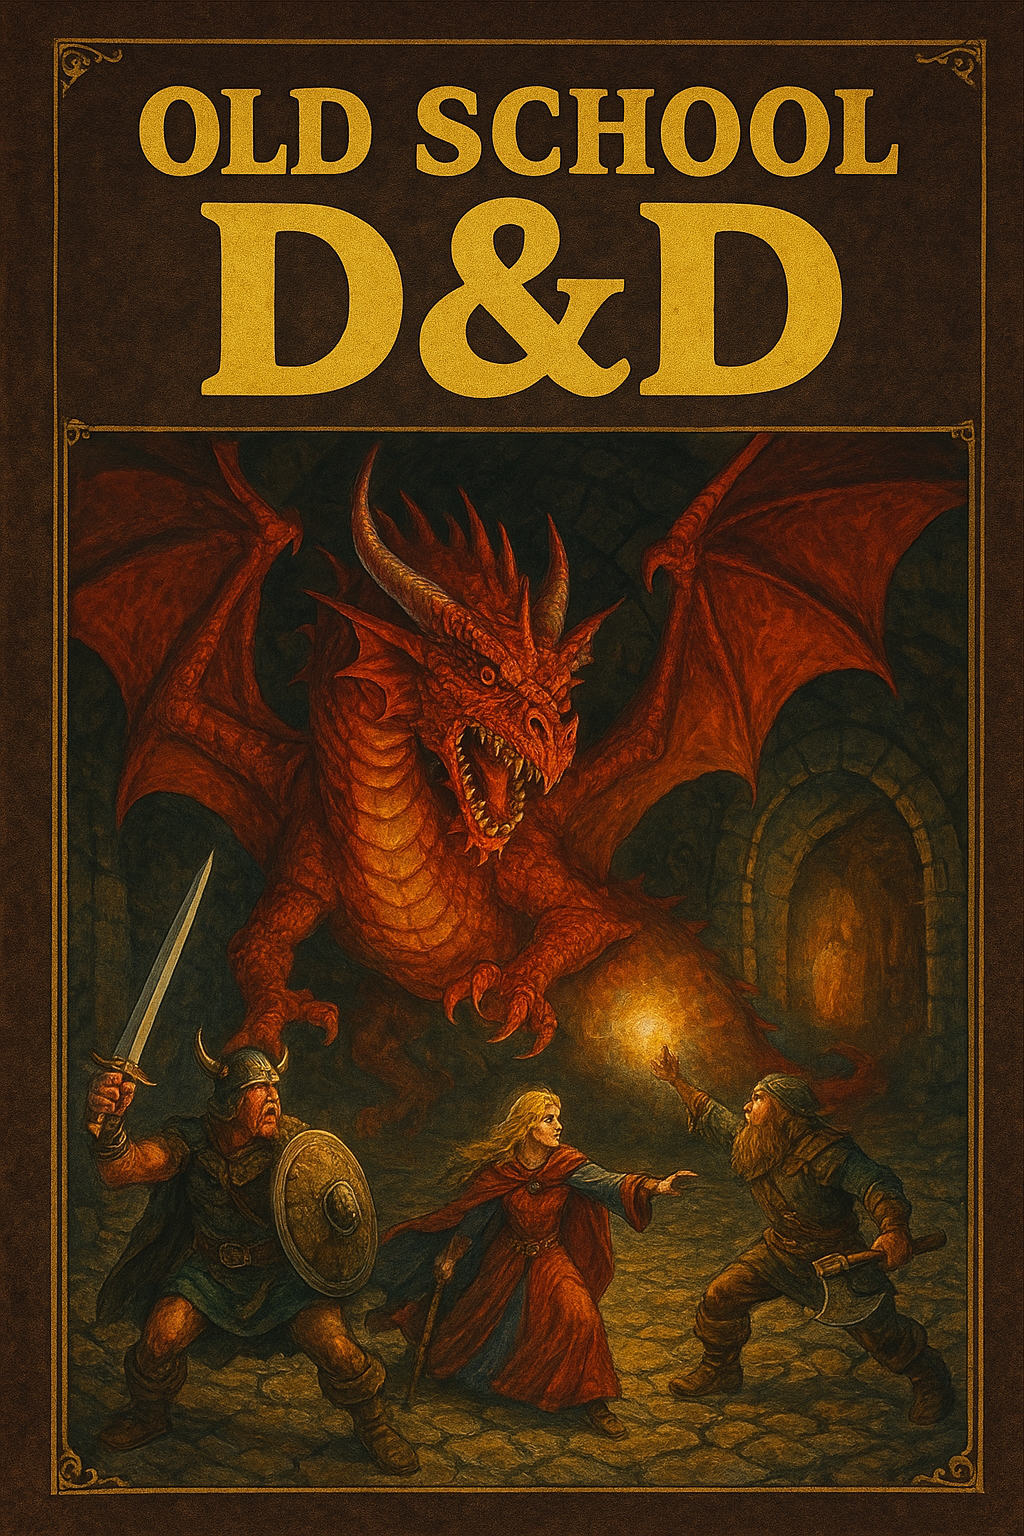
\includegraphics{./images/preface.pdf}

}

\caption{Old School D\&D}

\end{figure}%

Copyright and Usage Notice

Portions of this work make fair use of copyrighted material owned by
third parties, including game rules, terminology, and excerpts derived
from purchased products. Such use is made under the provisions of
Section 107 of the U.S. Copyright Act (Title 17, U.S. Code), which
permits limited use of copyrighted works for purposes such as
commentary, education, and fan creation. These materials are included
solely for non-commercial, transformative purposes, with no intent to
infringe upon or compete with the rights holders.

No part of this work may be sold, redistributed, or republished for
profit. Users may adapt or share excerpts for personal use only,
provided that attribution to the original author (Ryan Hartman) is
retained.

This website was created by Ryan Hartman, based on John Atom's
(jmhimara) original code.

\part{Introduction}

\chapter{Introduction}\label{introduction-1}

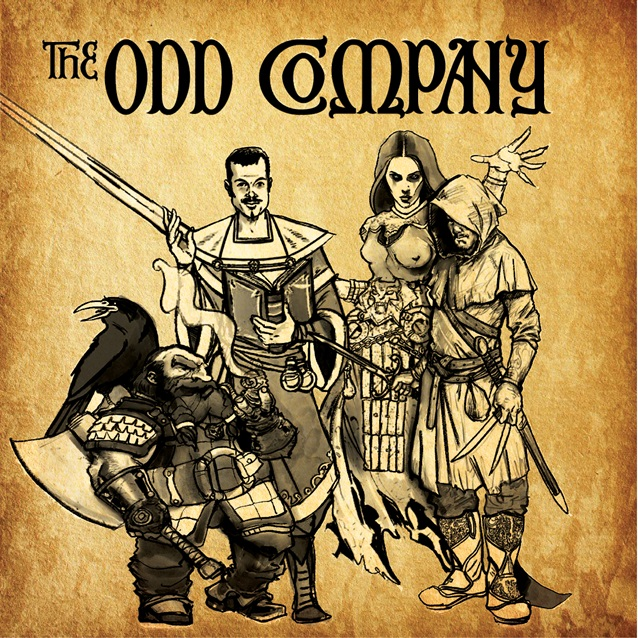
\includegraphics{./images/odd_company.jpg}

\emph{It was our first expedition into Drell's cursed mine in the
undercity beneath Minas Ithil. We stood before the ancient chamber
doors, where legend spoke of untold riches corrupted by the malevolent
blood of Xalara. I had scoffed at the tales whispered in the shadowy
corners of the city, but Harbek, the stalwart dwarf, believed every
word.}

\emph{Evron, the enigmatic magic-user, studied the intricate runes
etched into the door. ``These runes bear ancient magic,'' he murmured,
his voice tinged with curiosity rather than fear. ``They seem to ward
against trespassers.''}

\emph{Hunter Morgan, the agile thief, stepped forward, his eyes gleaming
with anticipation. ``Leave it to me,'' he grinned, deftly producing his
lockpicks. With a series of precise movements, he attempted to breach
the enchanted lock. To our surprise, the mechanism yielded with a soft
click.}

\emph{Galatea, the cleric of dubious allegiance, smirked knowingly.
``Magic bends to those who understand its nature,'' she remarked, her
eyes glinting with a hint of malice.}

\emph{As the doors swung open, revealing the dimly lit chamber within, a
chill wind whispered through the mine, carrying echoes of forgotten
whispers. Bones littered the ground around a stone sarcophagus, their
eerie presence casting long shadows across the ancient stone walls.}

\emph{Harbek's grip tightened on his battleaxe as he cautiously entered,
his eyes scanning the chamber for any sign of movement. ``Watch your
step,'' he grunted, his voice echoing in the oppressive silence.}

\emph{Evron approached the sarcophagus, his fingers tracing the
intricate carvings that adorned its surface. ``The lid looks heavy,'' he
observed thoughtfully. ``Let us turn it gently and reveal its secrets
without disturbing the restless dead.''}

\emph{Galatea's lips curled into a smile that sent shivers down my
spine. ``Fools,'' she hissed, her voice low and filled with dark
amusement. ``You dare to disturb the sanctum of the fallen?''}

\emph{Before anyone could react, the bones on the floor stirred,
rattling as if pulled by invisible strings. With unnatural speed, they
assembled themselves into skeletal warriors, their hollow sockets
glaring at us with malevolent intent. Gripping their ancient weapons,
they lunged forward, hungering for the warmth of the living.}

\emph{Evron cursed under his breath, summoning arcane energies to shield
us from the skeletal onslaught. Harbek roared a battle cry, swinging his
axe with deadly precision. Hunter Morgan darted among the shadows,
striking swift and silent blows.}

\emph{Galatea stood at the center of chaos, her dark laughter blending
with the clash of steel. ``Embrace the darkness,'' she taunted, her eyes
glowing with unholy fervor.}

\emph{As the battle raged on, each of us fought with a determination
born of survival. The mine echoed with the clash of weapons and the
cries of the undead. Amidst the chaos, I found myself wondering if our
greed had led us to this cursed place, or if fate had a more sinister
hand in our plight.}

\emph{In the end, it wasn't the lure of treasure that tested our mettle,
but the dark forces awakened by our trespass. And as the last echoes of
battle faded into silence, we stood victorious yet haunted, our hearts
heavy with the knowledge that some secrets are better left undisturbed
in the depths of Drell's cursed mine.}

\section{What Is This?}\label{what-is-this}

The \textbf{Basic Fantasy Role-Playing Game} is a rules-light game
system inspired by early role-playing game systems. It is intended for
fans of ``old-school'' game mechanics, simple enough for children in
second or third grade to play, yet offering enough depth for adults.

\section{What Is a Role-Playing
Game?}\label{what-is-a-role-playing-game}

In the almost 50 years since the first role-playing game appeared, much
has changed. Most people have at least heard of one or two such games,
and many have played. Still, some have not tried RPGs; if you are one of
those people, this part is for you.

Role-playing games are played by a number of players, commonly two to
eight, and a Dungeon Master (DM), who is responsible for running the
world, creating and managing the towns, nations, ruins, non-player
characters (NPCs), monsters, treasure, and all other elements that aid
or challenge the players. Dice are often used to determine the success
or failure of actions in the game; Basic Fantasy RPG uses polyhedral
dice for this purpose.

In essence, role-playing games are grown-up games of pretend, with rules
to determine outcomes. These rules range from very free-form and simple
to very complex and detailed.

This game attempts to balance simplicity and complexity, being neither
too detailed nor too free-form.

\section{What Do I Need to Play?}\label{what-do-i-need-to-play}

As a player, you should have a pencil, some notebook paper, and a set of
dice. Graph paper is also useful for drawing maps. You can use
preprinted character sheets available on the Basic Fantasy RPG website,
but notebook paper works fine.

As the Dungeon Master , you need the same materials. For new GMs or
those with limited preparation time, pre-written adventures (modules)
are available for free on the
\href{https://www.basicfantasy.org/}{basicfantasy.org} website. Modules
written for other game systems can also be used with some conversion.

\section{Using the Dice}\label{using-the-dice}

The 20-sided die (d20) is used to resolve attack rolls and saving
throws. The 10-sided die (d10) generates numbers from 1 to 10, and pairs
are used together to generate numbers from 1 to 100 (percentile rolls).
The 4-sided die (d4) is flipped rather than rolled. Other commonly used
dice include the 6-sided die (d6), 8-sided die (d8), and 12-sided die
(d12).

\part{Player Characters}

\chapter{Character Creation}\label{character-creation}

\section{How to Create a Player
Character}\label{how-to-create-a-player-character}

To begin creating your player character, you'll need a piece of paper to
record their statistics. You can use a preprinted character sheet if
available, or simply use a piece of notebook paper. An example character
is shown below. It's recommended to use a pencil for recording
information, as any statistic may change during play.

\hyperref[character-abilities]{Roll 3d6} for each ability score. Assign
the results to each ability, described in the
\hyperref[ability-scores]{Character Abilities} section, as desired.

Write down the ability score bonus (or penalty) for each score beside
the score itself, as shown on the table on the next page.

Next, choose a \hyperref[character-races]{race} and
\hyperref[character-classes]{class} for your character. Your character
must meet the Prime Requisite minimum for a class, as described in the
\hyperref[tbl-prime-requisites]{Character Classes} section, to be a
member of that class. Additionally, note that there are minimum (and
maximum) ability requirements for the various races, which must be met,
as described in the \hyperref[tbl-racial-requirements]{Character Races}
section.

\begin{figure}

\centering{

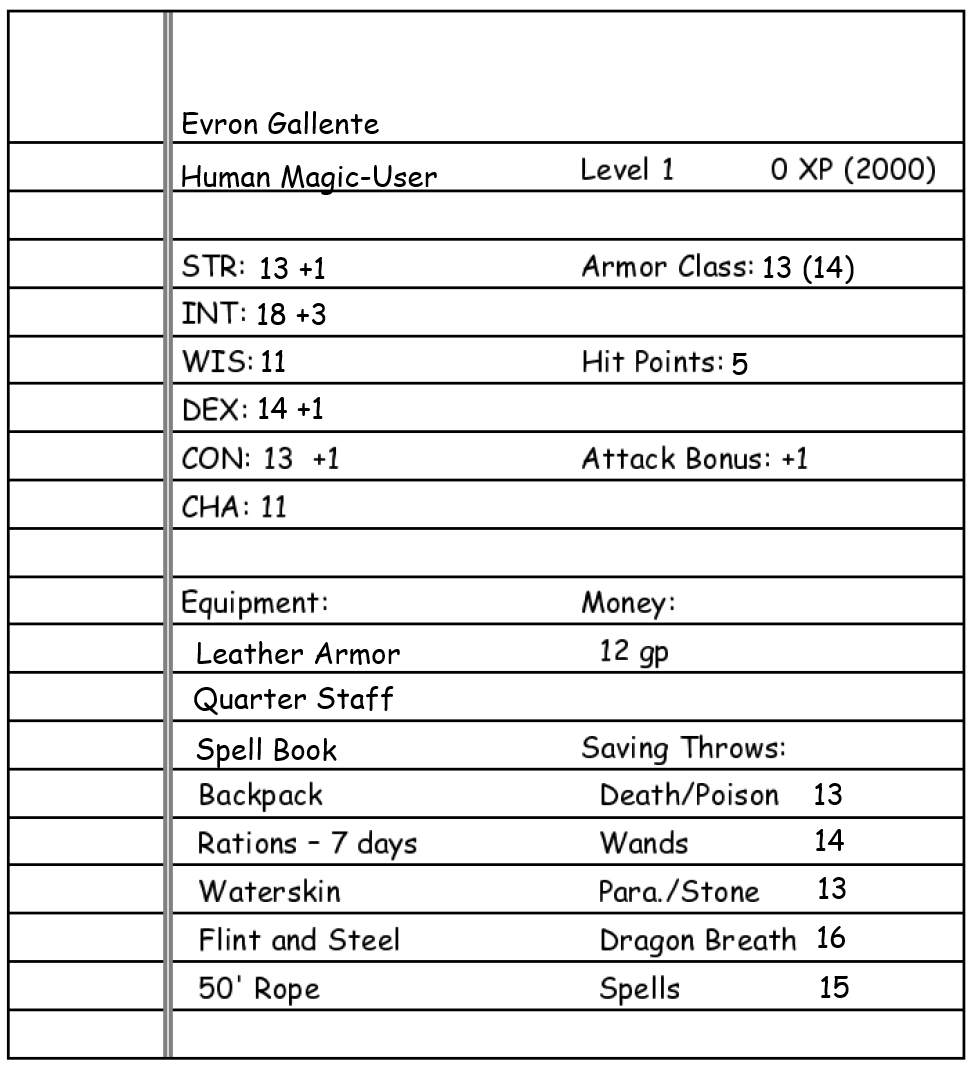
\includegraphics{./images/char.png}

}

\caption{\label{fig-char-info}Character Information}

\end{figure}%

Write down the special abilities of your race and class choices, as
described below. If you have chosen to play a Magic-User, ask your
Dungeon Master what spell or spells your character knows; it's up to the
Dungeon Master to decide this, but they may allow you to choose one or
more spells yourself.

Note on your character sheet that your character has zero (0) experience
points (or XP). Also, you may want to note the number needed to advance
to second level, as shown in the table for your class.

First-level characters begin play with the maximum HP for your class
plus your Constitution bonus or penalty. Note the result as your hit
points on your character sheet.

Roll for your starting money. Generally, your character will start with
3d6 times 10 gold pieces, but ask the Dungeon Master before rolling.
\hyperref[starting-gold]{Here} is an interactive tool to roll your
starting gold.

Now, purchase equipment for your character, as shown in the
\hyperref[equipment-explanations]{Equipment} section. Write your
purchases on your character sheet and note how much money remains
afterward. Ensure you understand the weapon and armor restrictions for
your class and race before making your purchases.
\hyperref[buy-equipment]{Here} is an interactive tool to purchase
equipment.

Since you now know what sort of armor your character is wearing, note
your Armor Class on your character sheet. Don't forget to add your
Dexterity bonus or penalty to the figure.

Look up your character's attack bonus (see
Table~\ref{tbl-attacking-bonus} in \href{combatDetails.qmd}{Encounters})
and note it on your character sheet. Don't add your ability bonuses (or
penalties) to this figure, as you will add a different bonus (Strength
or Dexterity) depending on the sort of weapon you use in combat (i.e.,
melee or missile weapon).

Also, look up your saving throws (from the tables near the end of the
\hyperref[saving-throw-tables-by-class]{Encounter} or at the appropriate
\hyperref[character-classes]{class}). Note them on your character sheet.
Adjust the saving throw figures based on your race, if your character is
a demi-human (see \href{races.qmd}{Character Races}). Please note that
the saving throw bonuses for demi-humans are presented as ``plus''
values, to be added to the die roll. For convenience, you may simply
subtract them from the saving throw numbers on the character sheet
instead.

Finally, if you haven't done so already, name your character. This often
takes longer than all the other steps combined.

\chapter{Character Abilities}\label{character-abilities}

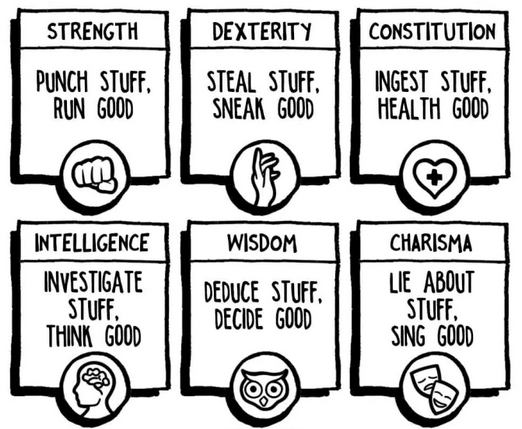
\includegraphics{images/abilities.png}

\section{Ability Scores}\label{ability-scores}

Each character will have a score ranging from 6 to 18 in each of the
following abilities. A bonus or penalty is associated with each score,
as shown on the table below. Each class has a
\hyperref[character-classes]{Prime Requisite} ability score, which must
be at least 9 for the character to become a member of that class.
Additionally, there are required minimum and maximum scores for each
character race other than Humans, as described under
\hyperref[character-races]{Character Races}.

\begin{longtable}[]{@{}
  >{\centering\arraybackslash}p{(\columnwidth - 2\tabcolsep) * \real{0.2778}}
  >{\centering\arraybackslash}p{(\columnwidth - 2\tabcolsep) * \real{0.2778}}@{}}
\caption{Ability Modifiers}\label{tbl-ability-modifiers}\tabularnewline
\toprule\noalign{}
\begin{minipage}[b]{\linewidth}\centering
\textbf{Ability Score}
\end{minipage} & \begin{minipage}[b]{\linewidth}\centering
\textbf{Bonus/Penalty}
\end{minipage} \\
\midrule\noalign{}
\endfirsthead
\toprule\noalign{}
\begin{minipage}[b]{\linewidth}\centering
\textbf{Ability Score}
\end{minipage} & \begin{minipage}[b]{\linewidth}\centering
\textbf{Bonus/Penalty}
\end{minipage} \\
\midrule\noalign{}
\endhead
\bottomrule\noalign{}
\endlastfoot
3 & -3 \\
4-5 & -2 \\
6-8 & -1 \\
9-12 & 0 \\
13-15 & +1 \\
16-17 & +2 \\
18 & +3 \\
19 & +4 \\
20 & +5 \\
\end{longtable}

\textbf{Strength:} This ability measures the character's raw physical
power. Strength is the Prime Requisite for \hyperref[fighter]{Fighters}.
Apply the ability bonus or penalty for Strength to all attack and damage
rolls in melee (hand-to-hand) combat. Note that a penalty here will not
reduce damage from a successful attack below one point in any case (see
the \hyperref[damage]{Combat} section for details).

\textbf{Intelligence:} This is the ability to learn and apply knowledge.
Intelligence is the Prime Requisite for
\hyperref[magic-users]{Magic-Users}, and they receive a Spell Bonus
based on their Intelligence score. The ability bonus for Intelligence is
added to the number of \hyperref[languages]{languages} the character can
learn to read and write. Characters with an Intelligence penalty may
struggle with learning languages, being limited to understanding only
their native language.

\textbf{Wisdom:} Wisdom is a combination of intuition, willpower, and
common sense. It is the Prime Requisite for \hyperref[cleric]{Clerics},
who receive a Spell Bonus and a bonus to Turn Undead based on their
Wisdom score. The Wisdom bonus or penalty may apply to some saving
throws vs.~magical attacks, particularly those affecting the target's
will.

\textbf{Dexterity:} This ability measures the character's quickness,
balance, and aptitude with tools. Dexterity is the Prime Requisite for
\hyperref[thief]{Thieves}. The Dexterity bonus or penalty applies to all
\hyperref[attacking-maneuvers]{attack rolls} with missile (ranged)
weapons, to the character's \hyperref[armor-and-shields]{Armor Class}
value, and to the character's \hyperref[initiative]{Initiative} die
roll.

\textbf{Constitution:} Constitution is a combination of general health
and vitality. Apply the Constitution bonus or penalty to each hit die
rolled by the character. Note that a penalty here will not reduce any
hit die roll to less than 1 point.

\textbf{Charisma:} This ability represents the character's ability to
influence or lead people. Those with high Charisma are well-liked or
highly respected. Apply the Charisma bonus or penalty to reaction rolls.
Also, the number of \hyperref[retainers]{retainers} a character can hire
and the loyalty of those retainers are affected by Charisma.

\subsubsection{Stat Roller}\label{stat-roller}

\begin{Shaded}
\begin{Highlighting}[]
\NormalTok{import \{ rollAbilityScore \} from "./custom.js"}

\NormalTok{viewof statRolls = Inputs.button(html\textasciigrave{}\textless{}button style="color: black; background{-}color: lightgray;"\textgreater{}Roll Stats\textless{}/button\textgreater{}\textasciigrave{}, \{value: null, reduce: () =\textgreater{} [rollAbilityScore(),rollAbilityScore(),rollAbilityScore(),rollAbilityScore(),rollAbilityScore(),rollAbilityScore()]\})}
\end{Highlighting}
\end{Shaded}

\begin{Shaded}
\begin{Highlighting}[]
\NormalTok{import \{ calculateModifier \} from "./custom.js"}
\NormalTok{\{}
\NormalTok{    var x = ""}
\NormalTok{    if (statRolls != null) \{}
\NormalTok{        x = html\textasciigrave{}\textless{}br\textgreater{}\textless{}table style="max{-}width:20\%;"\textgreater{}}
\NormalTok{                    \textless{}tr\textgreater{}}
\NormalTok{                        \textless{}td\textgreater{}$\{statRolls[0]\}\textless{}/td\textgreater{}}
\NormalTok{                        \textless{}td\textgreater{}($\{calculateModifier(statRolls[0])\})\textless{}/td\textgreater{}}
\NormalTok{                    \textless{}/tr\textgreater{}}
\NormalTok{                    \textless{}tr\textgreater{}}
\NormalTok{                        \textless{}td\textgreater{}$\{statRolls[1]\}\textless{}/td\textgreater{}}
\NormalTok{                        \textless{}td\textgreater{}($\{calculateModifier(statRolls[1])\})\textless{}/td\textgreater{}}
\NormalTok{                    \textless{}/tr\textgreater{}}
\NormalTok{                    \textless{}tr\textgreater{}}
\NormalTok{                        \textless{}td\textgreater{}$\{statRolls[2]\}\textless{}/td\textgreater{}}
\NormalTok{                        \textless{}td\textgreater{}($\{calculateModifier(statRolls[2])\})\textless{}/td\textgreater{}}
\NormalTok{                    \textless{}/tr\textgreater{}}
\NormalTok{                    \textless{}tr\textgreater{}}
\NormalTok{                        \textless{}td\textgreater{}$\{statRolls[3]\}\textless{}/td\textgreater{}}
\NormalTok{                        \textless{}td\textgreater{}($\{calculateModifier(statRolls[3])\})\textless{}/td\textgreater{}}
\NormalTok{                    \textless{}/tr\textgreater{}}
\NormalTok{                    \textless{}tr\textgreater{}}
\NormalTok{                        \textless{}td\textgreater{}$\{statRolls[4]\}\textless{}/td\textgreater{}}
\NormalTok{                        \textless{}td\textgreater{}($\{calculateModifier(statRolls[4])\})\textless{}/td\textgreater{}}
\NormalTok{                    \textless{}/tr\textgreater{}}
\NormalTok{                    \textless{}tr\textgreater{}}
\NormalTok{                        \textless{}td\textgreater{}$\{statRolls[5]\}\textless{}/td\textgreater{}}
\NormalTok{                        \textless{}td\textgreater{}($\{calculateModifier(statRolls[5])\})\textless{}/td\textgreater{}}
\NormalTok{                    \textless{}/tr\textgreater{}}
\NormalTok{                \textasciigrave{}}
\NormalTok{    \} else \{x = md\textasciigrave{}\textless{}br\textgreater{}\textless{}b\textgreater{}Press button to roll stats\textless{}b\textgreater{}\textasciigrave{}\}}

\NormalTok{    return x}
\NormalTok{    \} }
\end{Highlighting}
\end{Shaded}

\chapter{Character Races}\label{character-races}

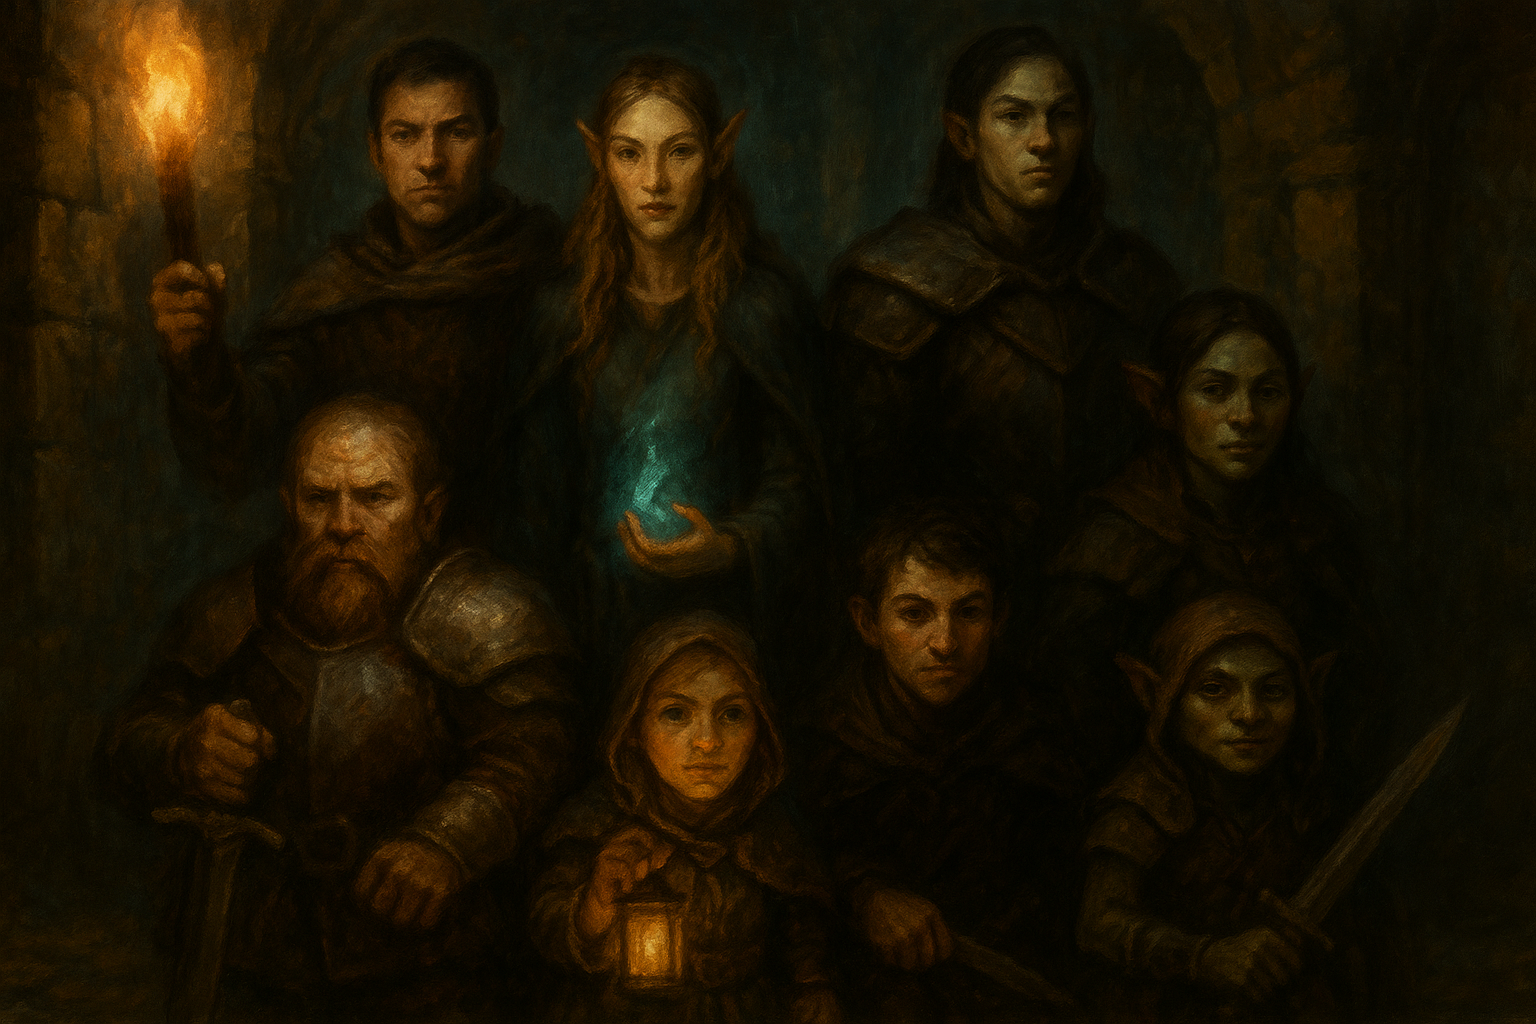
\includegraphics{images/races.png}

\section{Demography of OnceWas}\label{demography-of-oncewas}

The allowed PC character races in OnceWas are Human, Dwarf, Elf,
Half-Elf, or Halfling. Human is preferred for this campaign. In the
world of OnceWas, 80\% of the humanoid population is human, 5\% are
dwarves, 1.5\% are halflings, 1\% are elves, 0.5\% are half-elves, and
12\% are other races such as Orcs, Goblins, etc. It's important to note
that each race, except for Humans, has specific minimum and maximum
ability score requirements.

\begin{longtable}[]{@{}
  >{\raggedright\arraybackslash}p{(\columnwidth - 6\tabcolsep) * \real{0.1216}}
  >{\raggedright\arraybackslash}p{(\columnwidth - 6\tabcolsep) * \real{0.2162}}
  >{\raggedright\arraybackslash}p{(\columnwidth - 6\tabcolsep) * \real{0.2297}}
  >{\raggedright\arraybackslash}p{(\columnwidth - 6\tabcolsep) * \real{0.4324}}@{}}
\caption{Racial
Requirements}\label{tbl-racial-requirements}\tabularnewline
\toprule\noalign{}
\begin{minipage}[b]{\linewidth}\raggedright
Race
\end{minipage} & \begin{minipage}[b]{\linewidth}\raggedright
Min Score
\end{minipage} & \begin{minipage}[b]{\linewidth}\raggedright
Max Score
\end{minipage} & \begin{minipage}[b]{\linewidth}\raggedright
Classes
\end{minipage} \\
\midrule\noalign{}
\endfirsthead
\toprule\noalign{}
\begin{minipage}[b]{\linewidth}\raggedright
Race
\end{minipage} & \begin{minipage}[b]{\linewidth}\raggedright
Min Score
\end{minipage} & \begin{minipage}[b]{\linewidth}\raggedright
Max Score
\end{minipage} & \begin{minipage}[b]{\linewidth}\raggedright
Classes
\end{minipage} \\
\midrule\noalign{}
\endhead
\bottomrule\noalign{}
\endlastfoot
Dwarf & Constitution 9 & Charisma 17 & Cleric, Fighter, or Thief \\
Elf & Intelligence 9 & Constitution 17 & Any except Paladin \\
Half-Elf & Intelligence 9 & Constitution 17 & Any \\
Halfling & Dexterity 9 & Strength 17 & Cleric, Fighter, Ranger or
Thief \\
Human & None & None & Any \\
\end{longtable}

\section{Dwarves}\label{dwarves}

\textbf{Description:} Dwarves constitute 5\% of the population of
OnceWas. They are short, stocky beings with beards, typically standing
around four feet tall and weighing approximately 160 pounds. Their long
hair and thick beards come in dark brown, gray, or black hues. They take
great pride in their beards, often braiding or forking them. Dwarves
tend to have dark, ruddy complexions.

Renowned for their strength and hardiness, dwarves endure pain, fatigue,
and suffering better than most other races, boasting a lifespan of three
to four centuries. Despite their hardiness, they tend to appear old upon
reaching maturity.

Dwarves are skilled in blacksmithing, gem cutting, and craftwork,
particularly with materials like stone, gold, silver, and mithril. They
are typically known for their practicality, stubbornness, and courage,
though they can also be introspective, suspicious, and possessive.
Dwarves have a fondness for beer and ale.

Many Dwarven clans reside in Hammerfast, the Dwarvish Stronghold,
including the Battlehammer, Stoutaxes, Strongfellow, and Rockbrow
families.

\textbf{Restrictions:} Dwarves may pursue careers as Clerics, Fighters,
or Thieves. They must have a minimum Constitution score of 9. Due to
their generally dour dispositions, they may not possess a Charisma score
higher than 17. Additionally, dwarves are restricted from wielding Large
weapons exceeding four feet in length, such as two-handed swords,
polearms, and longbows.

Dwarves also incur a -10 feet penalty to combat movement.

\textbf{Special Abilities:} All Dwarves possess Darkvision with a range
of 60 feet and are adept at detecting slanting passages, traps, shifting
walls, and new constructions, gaining a +1 bonus on Investigation Skill
checks when examining and searching these features.

\textbf{Saving Throws:} Dwarves gain a +4 bonus against Death Ray or
Poison, Magic Wands, Paralysis or Petrify, and Spells, as well as a +3
bonus against Dragon Breath.

\section{Elves}\label{elves}

\textbf{Description:} The mysterious Elves make up 1\% of the
population. They are the oldest and wisest of the races of Oncewas. It
is said that the elves first arrived during the start of the Age of
Dragons, having traveled East across the Far Away Sea. They settled in
the Luisian Forest and built Imladris, the City of Elves. Elves are
practically immortal, noble, and fair.

Elves are a slender race, with both genders standing around five feet
tall and weighing around 130 pounds. Most have dark hair, with little or
no body or facial hair. Their skin is pale, and they have pointed ears
and delicate features. Elves are lithe and graceful, with keen eyesight
and hearing. They are typically inquisitive, passionate, self-assured,
and sometimes haughty. Their typical lifespan is a dozen centuries or
more. Elves do not sleep but instead enter trances for 4 hours a day in
which they remain semiconscious.

\textbf{Restrictions:} Elves may become \hyperref[cleric]{Clerics},
\hyperref[fighter]{Fighters}, \hyperref[magic-users]{Magic-Users}, or
\hyperref[thief]{Thieves}; they are also allowed to combine the classes
of Fighter and Magic-User, and of Magic-User and Thief (see
\hyperref[combination-classes]{Combination Classes}). They are required
to have a minimum Intelligence of 9. Due to their generally delicate
nature, they may not have a Constitution higher than 17. Elves never
roll larger than six-sided dice (d6) for hit points.

\textbf{Special Abilities:} All Elves have
\hyperref[darkvision]{Darkvision} with a 60' range. Elves are so
observant that they have an additional +1 on Perception Skill and Spot
Skills checks. Elves are immune to the paralyzing attack of ghouls, as
well as the Sleep spell. Elves are only surprised on a DC17 or better.
Elves also receive +10 feet to combat movement.

\textbf{Saving Throws:} Elves save at +1 vs.~Paralysis or Petrify, and
+2 vs.~Magic Wands and Spells.

\section{Half-Elves}\label{half-elves}

\textbf{Description:} Half-Elves make up 0.5\% of the population of
OnceWas. These beings combine the best parts of elves and humans, or so
they say. They don't really belong in either world, having to decide
which community they identify with more. For this reason, they work
excellently as ambassadors or wander off feeling excluded from all
places, sometimes in search of adventurers with whom they can find a
sense of belonging. An average Half-Elf male stands around 5'5'' in
height, with females averaging an inch shorter. They have pointed ears,
but their features tend to favor the Human parent a bit more than the
Elf. Half-elves live much longer than Humans, often exceeding 200 years.

\textbf{Restrictions:} Half-Elves may become members of any class or
combination allowed to Elves. They are required to have a minimum
Intelligence of 9, and like Elves, they may not have Constitution scores
higher than 17. They do not suffer from the Elven hit dice limit.

\textbf{Special Abilities:} Half-Elves have
\hyperref[darkvision]{Darkvision} with a 30' range. They also have an
additional +1 on Perception Skill checks. Half-Elves gain a bonus of
+5\% on all earned experience, unless a member of a combination class.

\textbf{Saving Throws:} Half-Elves save at +1 vs.~Magic Wands and
Spells.

\section{Halflings}\label{halflings}

\textbf{Description:} Halflings make up 1.5\% of the population of
OnceWas. They are isolated, cheerful people who love the comfort of
their homes and communities, which is why most of them don't stray from
their shires. However, a strong sense of curiosity inhabits many of
them, leading some of these little folk to become adventurers or travel
to other places. They are extremely agile, but due to their short legs,
they are not as fast as other races. Halflings are good-natured,
hospitable, and easygoing folk, three to four feet in height and
weighing about 60 pounds. They have curly brown hair on their heads and
feet, but rarely have facial hair. They are usually fair-skinned, often
with ruddy cheeks. Halflings are remarkably rugged for their small size.
They are dexterous and nimble, capable of moving quietly and remaining
very still. They usually go barefoot. Halflings have lifespans
comparable to, but slightly longer than, humans. A halfling is typically
considered an adult in their early twenties, and some live into their
150s.

\textbf{Restrictions:} Halflings may become \hyperref[cleric]{Clerics},
\hyperref[fighter]{Fighters}, or \hyperref[thief]{Thieves}. They are
required to have a minimum Dexterity of 9. Due to their small stature,
they may not have a Strength higher than 17. Halflings never roll larger
than six-sided dice (d6) for hit points regardless of class. Halflings
may not use Large weapons and must wield Medium weapons with both hands.

\textbf{Special Abilities:} Halflings are unusually accurate with all
sorts of ranged weapons, gaining a +1 attack bonus when employing them.
When attacked in melee by creatures larger than man-sized, Halflings
gain a +2 bonus to their Armor Class. Halflings are quick-witted, thus
adding +1 to \hyperref[initiative]{Initiative} die rolls. Halflings can
hide in shadows indoors like the \hyperref[thief]{Thief} ability and
hide outdoors like the \hyperref[ranger]{Ranger} ability of the same
level.

\textbf{Saving Throws:} Halflings save at +4 vs.~Death Ray or Poison,
Magic Wands, Paralysis or Petrify, and Spells, and at +3 vs.~Dragon
Breath.

\section{Humans}\label{humans}

\textbf{Description:} Humans make up 80\% of the population of OnceWas.
They come in a broad variety of shapes and sizes. The towering
barbarians of Stonehold would seem to have very little in common with
the desert dwellers of Sunndi. An average human male in good health
stands just less than six feet tall and weighs about 175 pounds. Most
humans in OnceWas live around 80 years.

\textbf{Restrictions:} Humans may choose any single class. They have no
minimum or maximum ability score requirements.

\textbf{Special Abilities:} Humans learn unusually quickly, gaining a
bonus of 10\% to all experience points earned.

\textbf{Saving Throws:} Humans are considered the ``standard,'' and thus
have no saving throw bonuses.

\chapter{Character Classes}\label{character-classes}

The available classes are Cleric, Druid, Fighter, Paladin, Ranger,
Magic-User, and Thief. To be a member of a class, a character must meet
the specified Prime Requisite minimum and racial requirements for that
class.

\begin{longtable}[]{@{}ll@{}}
\caption{Class Prime
Requisites}\label{tbl-prime-requisites}\tabularnewline
\toprule\noalign{}
Class & Minimum Scores \\
\midrule\noalign{}
\endfirsthead
\toprule\noalign{}
Class & Minimum Scores \\
\midrule\noalign{}
\endhead
\bottomrule\noalign{}
\endlastfoot
Cleric or Druid & Wisdom 9 \\
Figther & Strength 9 \\
Ranger & Strength 9, Wisdom 11, Dexterity 11 \\
Paladin & Strength 9, Wisdom 11, Charisma 11 \\
Magic-User & Intelligence 9 \\
Thief & Dexterity 9 \\
Fighter/Magic-User & Strength 9, Intelligence 9 \\
Magic-User/Thief & Intelligence 9, Dexterity 9 \\
\end{longtable}

\section{Cleric}\label{cleric}

\begin{center}

\includegraphics[width=2.08333in,height=\textheight]{images/cleric_class.png}
\end{center}

Clerics have devoted themselves to the service of a
\href{gods.qmd}{deity}. Additionally, there are twelve demigods and
twelve Demon Lords. Clerics of demigods and Demon Lords cannot advance
beyond 6\textsuperscript{th} level.

Most Clerics spend their time in mundane forms of service, such as
preaching and ministering at a temple. A select few are called to travel
away from the temple and serve their deity more directly, smiting undead
monsters and aiding in the battle against evil and chaos. Player Clerics
are assumed to be among this group.

Clerics fight about as well as Thieves but not as well as Fighters. They
are hardier than Thieves, at least at lower levels, as they are
accustomed to physical labor that the Thief would deftly avoid. Clerics
can cast \hyperref[cleric-spells]{spells of divine nature} starting at
2\textsuperscript{nd} level, and they have the power to Turn the Undead,
driving away undead monsters by means of faith alone (see the
\hyperref[turning-the-undead]{Encounter} section for details).

The Prime Requisite for Clerics is Wisdom; a character must have a
Wisdom score of 9 or higher to become a Cleric. They may wear any armor
and have no weapon restrictions.

\begin{center}
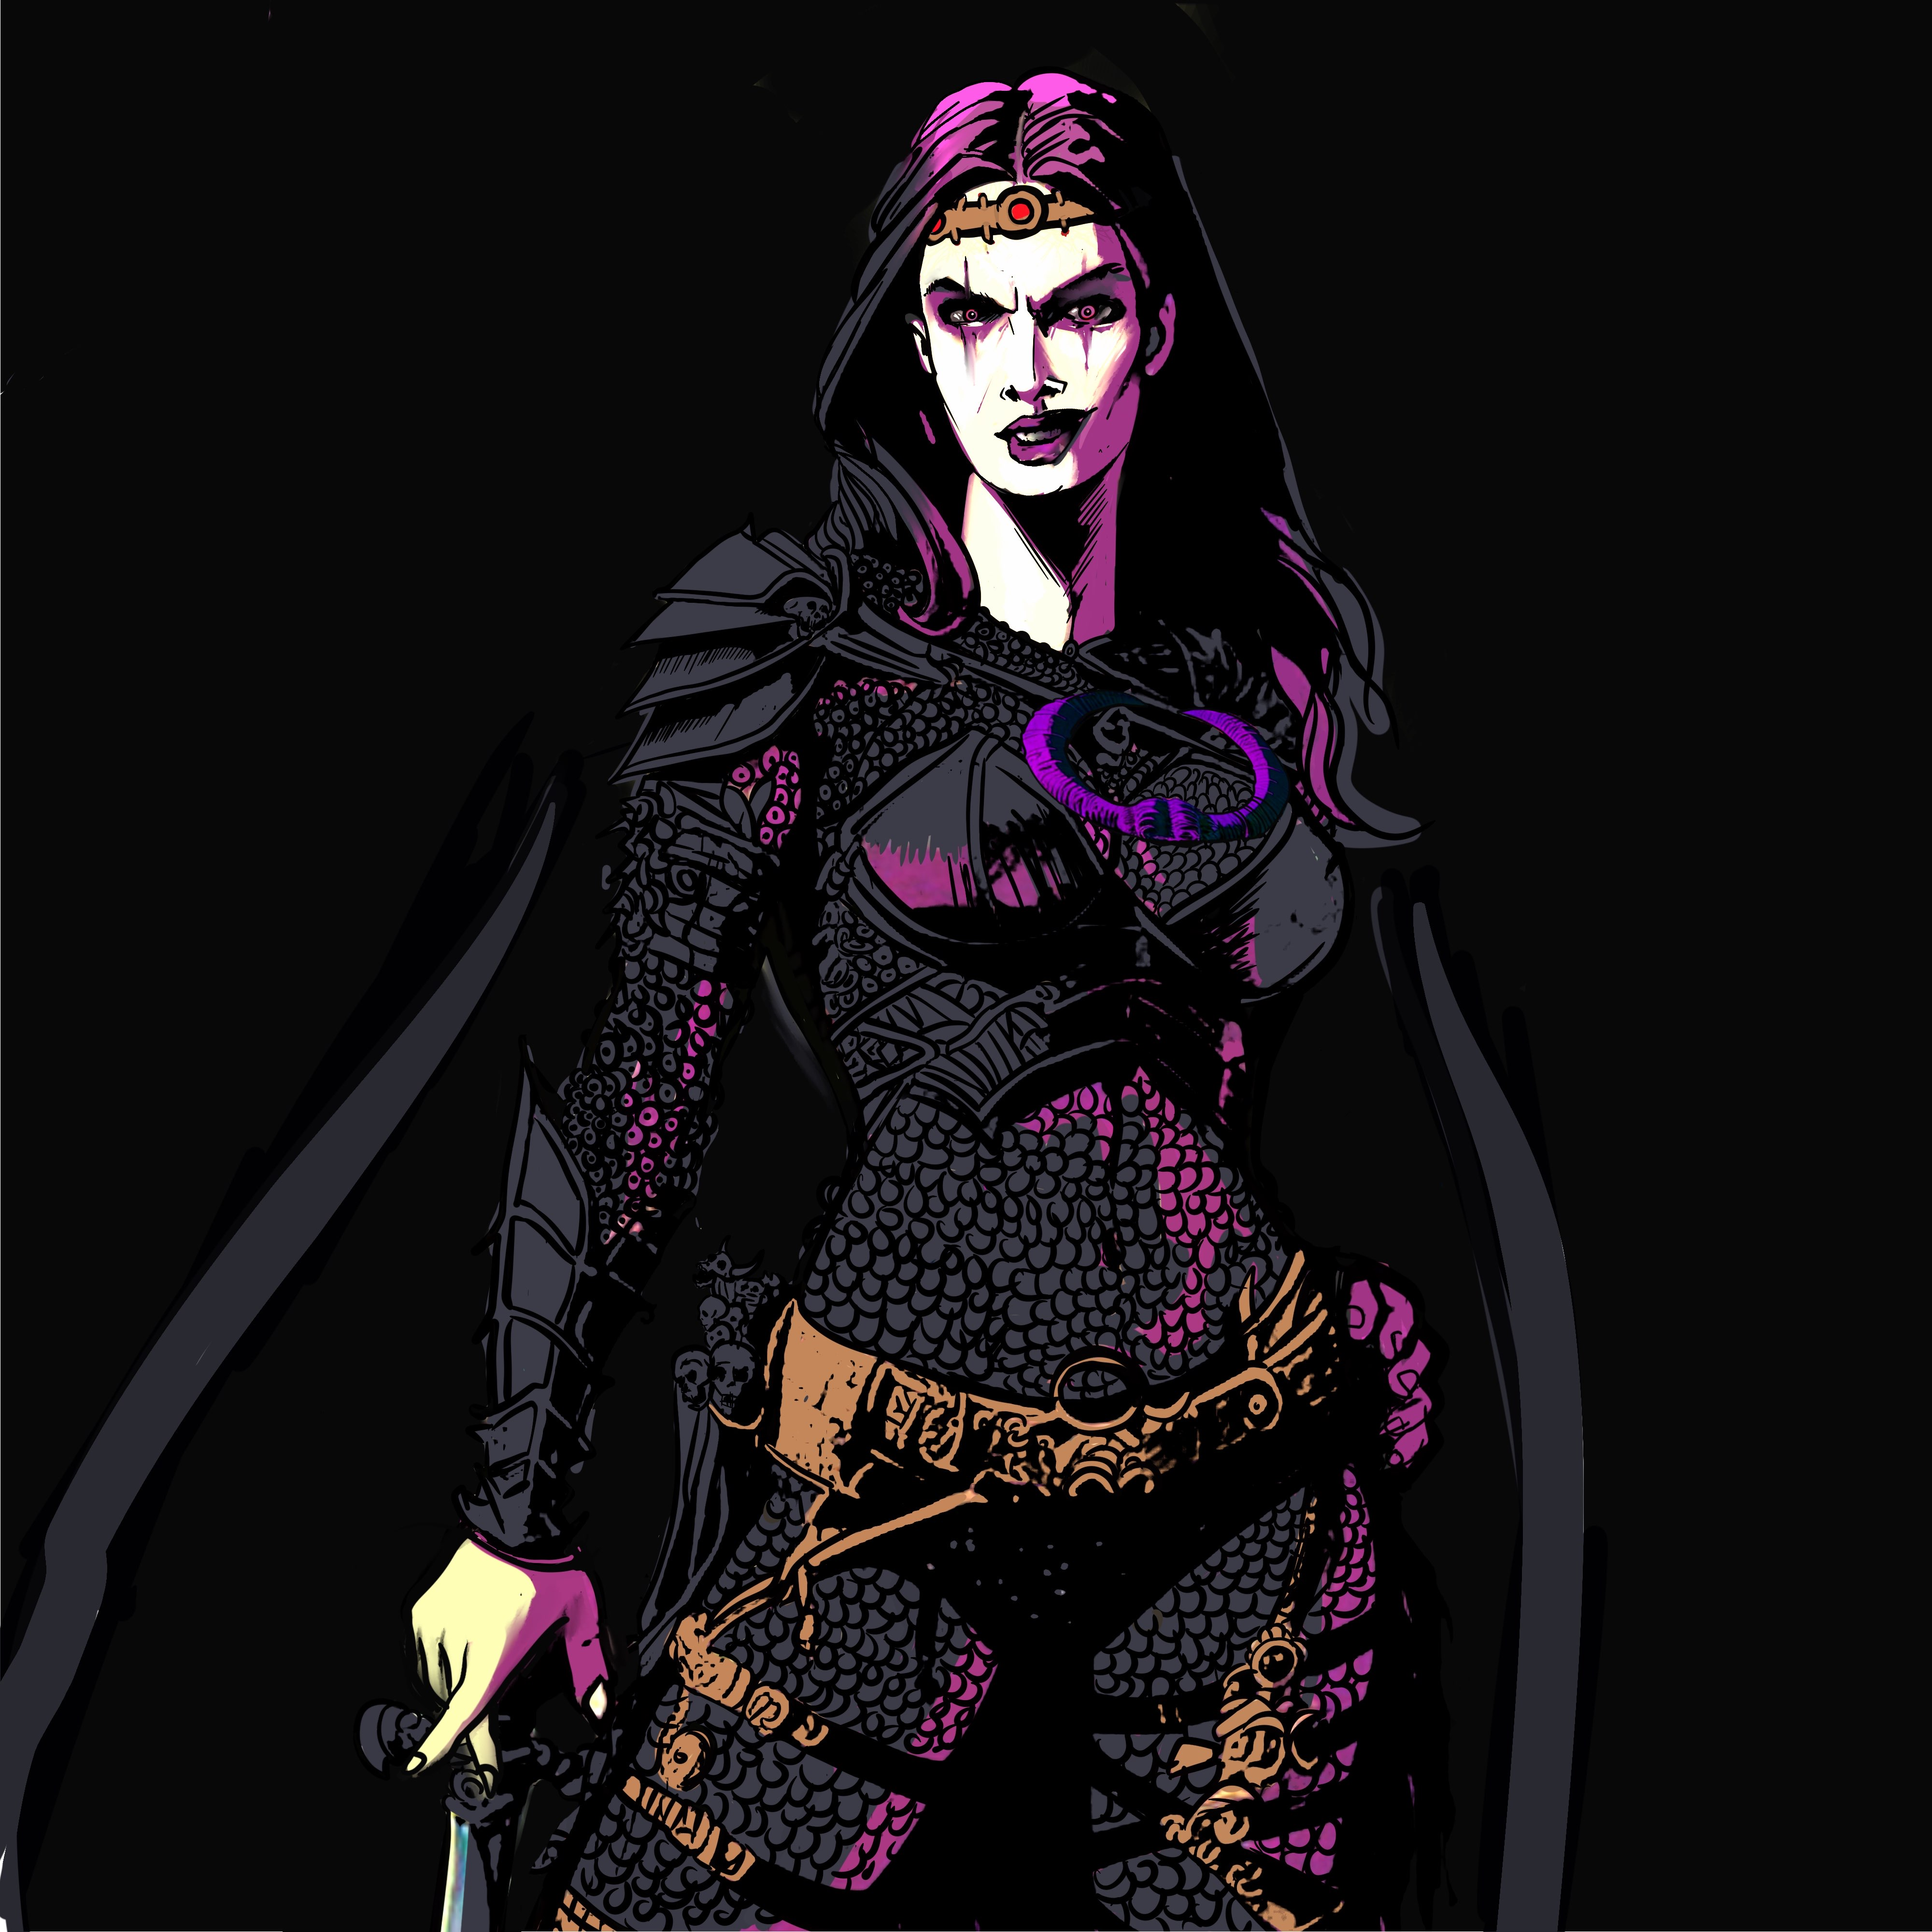
\includegraphics{images/cleric.jpg}
\end{center}

\begin{figure*}

\begin{longtable}[]{@{}
  >{\raggedright\arraybackslash}p{(\columnwidth - 28\tabcolsep) * \real{0.0630}}
  >{\raggedleft\arraybackslash}p{(\columnwidth - 28\tabcolsep) * \real{0.1102}}
  >{\centering\arraybackslash}p{(\columnwidth - 28\tabcolsep) * \real{0.0866}}
  >{\centering\arraybackslash}p{(\columnwidth - 28\tabcolsep) * \real{0.0787}}
  >{\centering\arraybackslash}p{(\columnwidth - 28\tabcolsep) * \real{0.0866}}
  >{\centering\arraybackslash}p{(\columnwidth - 28\tabcolsep) * \real{0.0866}}
  >{\raggedright\arraybackslash}p{(\columnwidth - 28\tabcolsep) * \real{0.0315}}
  >{\raggedright\arraybackslash}p{(\columnwidth - 28\tabcolsep) * \real{0.0315}}
  >{\raggedright\arraybackslash}p{(\columnwidth - 28\tabcolsep) * \real{0.0315}}
  >{\raggedright\arraybackslash}p{(\columnwidth - 28\tabcolsep) * \real{0.0315}}
  >{\raggedright\arraybackslash}p{(\columnwidth - 28\tabcolsep) * \real{0.0315}}
  >{\raggedright\arraybackslash}p{(\columnwidth - 28\tabcolsep) * \real{0.0315}}
  >{\raggedright\arraybackslash}p{(\columnwidth - 28\tabcolsep) * \real{0.0315}}
  >{\raggedright\arraybackslash}p{(\columnwidth - 28\tabcolsep) * \real{0.0315}}
  >{\centering\arraybackslash}p{(\columnwidth - 28\tabcolsep) * \real{0.1339}}@{}}
\caption{Cleric XP Progression}\label{tbl-xp-clerics}\tabularnewline
\toprule\noalign{}
\begin{minipage}[b]{\linewidth}\raggedright
\end{minipage} & \begin{minipage}[b]{\linewidth}\raggedleft
\end{minipage} & \begin{minipage}[b]{\linewidth}\centering
\end{minipage} & \begin{minipage}[b]{\linewidth}\centering
\end{minipage} & \begin{minipage}[b]{\linewidth}\centering
\end{minipage} & \begin{minipage}[b]{\linewidth}\centering
\end{minipage} & \begin{minipage}[b]{\linewidth}\raggedright
\end{minipage} & \begin{minipage}[b]{\linewidth}\raggedright
\end{minipage} &
\multicolumn{4}{>{\raggedright\arraybackslash}p{(\columnwidth - 28\tabcolsep) * \real{0.1260} + 6\tabcolsep}}{%
\begin{minipage}[b]{\linewidth}\raggedright
Spell Level
\end{minipage}} & \begin{minipage}[b]{\linewidth}\raggedright
\end{minipage} & \begin{minipage}[b]{\linewidth}\raggedright
\end{minipage} & \begin{minipage}[b]{\linewidth}\centering
\end{minipage} \\
\begin{minipage}[b]{\linewidth}\raggedright
Level
\end{minipage} & \begin{minipage}[b]{\linewidth}\raggedleft
Exp. Points
\end{minipage} & \begin{minipage}[b]{\linewidth}\centering
Hit Dice
\end{minipage} & \begin{minipage}[b]{\linewidth}\centering
Attack Bonus
\end{minipage} & \begin{minipage}[b]{\linewidth}\centering
Skill Points
\end{minipage} & \begin{minipage}[b]{\linewidth}\centering
Feats
\end{minipage} & \begin{minipage}[b]{\linewidth}\raggedright
0
\end{minipage} & \begin{minipage}[b]{\linewidth}\raggedright
1
\end{minipage} & \begin{minipage}[b]{\linewidth}\raggedright
2
\end{minipage} & \begin{minipage}[b]{\linewidth}\raggedright
3
\end{minipage} & \begin{minipage}[b]{\linewidth}\raggedright
4
\end{minipage} & \begin{minipage}[b]{\linewidth}\raggedright
5
\end{minipage} & \begin{minipage}[b]{\linewidth}\raggedright
6
\end{minipage} & \begin{minipage}[b]{\linewidth}\raggedright
7
\end{minipage} & \begin{minipage}[b]{\linewidth}\centering
Weapon Proficiency
\end{minipage} \\
\midrule\noalign{}
\endfirsthead
\toprule\noalign{}
\begin{minipage}[b]{\linewidth}\raggedright
\end{minipage} & \begin{minipage}[b]{\linewidth}\raggedleft
\end{minipage} & \begin{minipage}[b]{\linewidth}\centering
\end{minipage} & \begin{minipage}[b]{\linewidth}\centering
\end{minipage} & \begin{minipage}[b]{\linewidth}\centering
\end{minipage} & \begin{minipage}[b]{\linewidth}\centering
\end{minipage} & \begin{minipage}[b]{\linewidth}\raggedright
\end{minipage} & \begin{minipage}[b]{\linewidth}\raggedright
\end{minipage} &
\multicolumn{4}{>{\raggedright\arraybackslash}p{(\columnwidth - 28\tabcolsep) * \real{0.1260} + 6\tabcolsep}}{%
\begin{minipage}[b]{\linewidth}\raggedright
Spell Level
\end{minipage}} & \begin{minipage}[b]{\linewidth}\raggedright
\end{minipage} & \begin{minipage}[b]{\linewidth}\raggedright
\end{minipage} & \begin{minipage}[b]{\linewidth}\centering
\end{minipage} \\
\begin{minipage}[b]{\linewidth}\raggedright
Level
\end{minipage} & \begin{minipage}[b]{\linewidth}\raggedleft
Exp. Points
\end{minipage} & \begin{minipage}[b]{\linewidth}\centering
Hit Dice
\end{minipage} & \begin{minipage}[b]{\linewidth}\centering
Attack Bonus
\end{minipage} & \begin{minipage}[b]{\linewidth}\centering
Skill Points
\end{minipage} & \begin{minipage}[b]{\linewidth}\centering
Feats
\end{minipage} & \begin{minipage}[b]{\linewidth}\raggedright
0
\end{minipage} & \begin{minipage}[b]{\linewidth}\raggedright
1
\end{minipage} & \begin{minipage}[b]{\linewidth}\raggedright
2
\end{minipage} & \begin{minipage}[b]{\linewidth}\raggedright
3
\end{minipage} & \begin{minipage}[b]{\linewidth}\raggedright
4
\end{minipage} & \begin{minipage}[b]{\linewidth}\raggedright
5
\end{minipage} & \begin{minipage}[b]{\linewidth}\raggedright
6
\end{minipage} & \begin{minipage}[b]{\linewidth}\raggedright
7
\end{minipage} & \begin{minipage}[b]{\linewidth}\centering
Weapon Proficiency
\end{minipage} \\
\midrule\noalign{}
\endhead
\bottomrule\noalign{}
\endlastfoot
1 & 0 & 1d8 & +1 & 3 & & 1 & -- & -- & -- & -- & -- & -- & -- & 3 \\
2 & 1,500 & 2d8 & +1 & 1 & 1 & 2 & 1 & -- & -- & -- & -- & -- & -- & \\
3 & 3,000 & 3d8 & +2 & 1 & & 3 & 2 & -- & -- & -- & -- & -- & -- & \\
4 & 6,000 & 4d8 & +2 & 1 & 1 & 4 & 2 & 1 & -- & -- & -- & -- & -- & 1 \\
5 & 12,000 & 5d8 & +3 & 1 & & 5 & 2 & 2 & -- & -- & -- & -- & -- & \\
6 & 24,000 & 6d8 & +3 & 1 & 1 & 6 & 2 & 2 & 1 & -- & -- & -- & -- & \\
7 & 48,000 & 7d8 & +4 & 1 & & 7 & 3 & 2 & 2 & -- & -- & -- & -- & 1 \\
8 & 90,000 & 8d8 & +4 & 1 & 1 & 8 & 3 & 2 & 2 & 1 & -- & -- & -- & \\
9 & 180,000 & 9d8 & +5 & 1 & & 9 & 3 & 3 & 2 & 2 & -- & -- & -- & \\
10 & 270,000 & 9d8+1 & +5 & 1 & 1 & 9 & 3 & 3 & 2 & 2 & 1 & -- & -- &
1 \\
11 & 360,000 & 9d8+2 & +5 & 1 & & 9 & 4 & 3 & 3 & 2 & 2 & -- & -- & \\
12 & 450,000 & 9d8+3 & +6 & 1 & 1 & 9 & 4 & 4 & 3 & 2 & 2 & 1 & -- & \\
13 & 540,000 & 9d8+4 & +6 & 1 & & 9 & 4 & 4 & 3 & 3 & 2 & 2 & -- & 1 \\
14 & 630,000 & 9d8+5 & +6 & 1 & 1 & 9 & 4 & 4 & 4 & 3 & 2 & 2 & 1 & \\
15 & 720,000 & 9d8+6 & +7 & 1 & & 9 & 4 & 4 & 4 & 3 & 3 & 2 & 1 & \\
16 & 810,000 & 9d8+7 & +7 & 1 & 1 & 9 & 5 & 4 & 4 & 3 & 3 & 2 & 1 & 1 \\
17 & 900,000 & 9d8+8 & +7 & 1 & & 9 & 5 & 5 & 4 & 3 & 3 & 2 & 2 & \\
18 & 990,000 & 9d8+9 & +8 & 1 & 1 & 9 & 5 & 5 & 4 & 4 & 3 & 3 & 2 & \\
19 & 1,080,000 & 9d8+10 & +8 & 1 & & 9 & 6 & 5 & 4 & 4 & 3 & 3 & 2 &
1 \\
20 & 1,170,000 & 9d8+11 & +8 & 1 & 1 & 9 & 6 & 5 & 4 & 4 & 3 & 3 & 3
& \\
\end{longtable}

\end{figure*}%

\begin{longtable}[]{@{}ll@{}}
\caption{Cleric Wisdom Bonus}\label{tbl-wisdom-clerics}\tabularnewline
\toprule\noalign{}
Wisdom & Spell Bonus \\
\midrule\noalign{}
\endfirsthead
\toprule\noalign{}
Wisdom & Spell Bonus \\
\midrule\noalign{}
\endhead
\bottomrule\noalign{}
\endlastfoot
9-11 & No bonus spells \\
12 & +1 Orison \\
13-15 & +1 Orison, +1 1\textsuperscript{st} level spell \\
16-17 & +2 Orisons, +2 1\textsuperscript{st} level spells \\
18 & +3 Orisons, +3 1\textsuperscript{st} level, +1
2\textsuperscript{nd} level spells \\
\end{longtable}

\begin{figure*}

\begin{longtable}[]{@{}
  >{\raggedright\arraybackslash}p{(\columnwidth - 16\tabcolsep) * \real{0.0833}}
  >{\raggedright\arraybackslash}p{(\columnwidth - 16\tabcolsep) * \real{0.0833}}
  >{\raggedright\arraybackslash}p{(\columnwidth - 16\tabcolsep) * \real{0.0833}}
  >{\raggedright\arraybackslash}p{(\columnwidth - 16\tabcolsep) * \real{0.0833}}
  >{\raggedright\arraybackslash}p{(\columnwidth - 16\tabcolsep) * \real{0.1136}}
  >{\raggedright\arraybackslash}p{(\columnwidth - 16\tabcolsep) * \real{0.1136}}
  >{\raggedright\arraybackslash}p{(\columnwidth - 16\tabcolsep) * \real{0.1364}}
  >{\raggedright\arraybackslash}p{(\columnwidth - 16\tabcolsep) * \real{0.1288}}
  >{\raggedright\arraybackslash}p{(\columnwidth - 16\tabcolsep) * \real{0.1742}}@{}}
\caption{Cleric Titles}\label{tbl-titles-clerics}\tabularnewline
\toprule\noalign{}
\begin{minipage}[b]{\linewidth}\raggedright
Alignment
\end{minipage} & \begin{minipage}[b]{\linewidth}\raggedright
Level 1
\end{minipage} & \begin{minipage}[b]{\linewidth}\raggedright
Level 2
\end{minipage} & \begin{minipage}[b]{\linewidth}\raggedright
Level 3
\end{minipage} & \begin{minipage}[b]{\linewidth}\raggedright
Level 4
\end{minipage} & \begin{minipage}[b]{\linewidth}\raggedright
Level 5
\end{minipage} & \begin{minipage}[b]{\linewidth}\raggedright
Level 9
\end{minipage} & \begin{minipage}[b]{\linewidth}\raggedright
Level 12
\end{minipage} & \begin{minipage}[b]{\linewidth}\raggedright
Level 15
\end{minipage} \\
\midrule\noalign{}
\endfirsthead
\toprule\noalign{}
\begin{minipage}[b]{\linewidth}\raggedright
Alignment
\end{minipage} & \begin{minipage}[b]{\linewidth}\raggedright
Level 1
\end{minipage} & \begin{minipage}[b]{\linewidth}\raggedright
Level 2
\end{minipage} & \begin{minipage}[b]{\linewidth}\raggedright
Level 3
\end{minipage} & \begin{minipage}[b]{\linewidth}\raggedright
Level 4
\end{minipage} & \begin{minipage}[b]{\linewidth}\raggedright
Level 5
\end{minipage} & \begin{minipage}[b]{\linewidth}\raggedright
Level 9
\end{minipage} & \begin{minipage}[b]{\linewidth}\raggedright
Level 12
\end{minipage} & \begin{minipage}[b]{\linewidth}\raggedright
Level 15
\end{minipage} \\
\midrule\noalign{}
\endhead
\bottomrule\noalign{}
\endlastfoot
Lawful & Acolyte & Adept & Priest & Vicar & Curate & High Priest &
Bishop & Patriarch/Matriarch \\
Neutral & Seeker & Devotee & Guardian & Shaman & Guide & Elder &
Hierarch & Oracle \\
Chaotic & Initiate & Zealot & Cultist & Ravager & Doomcaller &
Blightbringer & Shadow Prophet & Chaos Lord/Lady \\
\end{longtable}

\end{figure*}%

\begin{longtable}[]{@{}
  >{\raggedright\arraybackslash}p{(\columnwidth - 10\tabcolsep) * \real{0.1250}}
  >{\raggedright\arraybackslash}p{(\columnwidth - 10\tabcolsep) * \real{0.2273}}
  >{\raggedright\arraybackslash}p{(\columnwidth - 10\tabcolsep) * \real{0.1477}}
  >{\raggedright\arraybackslash}p{(\columnwidth - 10\tabcolsep) * \real{0.2386}}
  >{\raggedright\arraybackslash}p{(\columnwidth - 10\tabcolsep) * \real{0.1705}}
  >{\raggedright\arraybackslash}p{(\columnwidth - 10\tabcolsep) * \real{0.0909}}@{}}
\caption{Cleric Saving Throws}\label{tbl-save-clerics}\tabularnewline
\toprule\noalign{}
\begin{minipage}[b]{\linewidth}\raggedright
\textbf{Level}
\end{minipage} & \begin{minipage}[b]{\linewidth}\raggedright
Death Ray / Poison
\end{minipage} & \begin{minipage}[b]{\linewidth}\raggedright
Magic Wands
\end{minipage} & \begin{minipage}[b]{\linewidth}\raggedright
Paralysis / Petrify
\end{minipage} & \begin{minipage}[b]{\linewidth}\raggedright
Dragon Breath
\end{minipage} & \begin{minipage}[b]{\linewidth}\raggedright
Spells
\end{minipage} \\
\midrule\noalign{}
\endfirsthead
\toprule\noalign{}
\begin{minipage}[b]{\linewidth}\raggedright
\textbf{Level}
\end{minipage} & \begin{minipage}[b]{\linewidth}\raggedright
Death Ray / Poison
\end{minipage} & \begin{minipage}[b]{\linewidth}\raggedright
Magic Wands
\end{minipage} & \begin{minipage}[b]{\linewidth}\raggedright
Paralysis / Petrify
\end{minipage} & \begin{minipage}[b]{\linewidth}\raggedright
Dragon Breath
\end{minipage} & \begin{minipage}[b]{\linewidth}\raggedright
Spells
\end{minipage} \\
\midrule\noalign{}
\endhead
\bottomrule\noalign{}
\endlastfoot
\textbf{1} & 11 & 12 & 14 & 16 & 15 \\
\textbf{2-3} & 10 & 11 & 13 & 15 & 14 \\
\textbf{4-5} & 9 & 10 & 13 & 15 & 14 \\
\textbf{6-7} & 9 & 10 & 12 & 14 & 13 \\
\textbf{8-9} & 8 & 9 & 12 & 14 & 13 \\
\textbf{10-11} & 8 & 9 & 11 & 13 & 12 \\
\textbf{12-13} & 7 & 8 & 11 & 13 & 12 \\
\textbf{14-15} & 7 & 8 & 10 & 12 & 11 \\
\textbf{16-17} & 6 & 7 & 10 & 12 & 11 \\
\textbf{18-19} & 6 & 7 & 9 & 11 & 10 \\
\textbf{20} & 5 & 6 & 9 & 11 & 10 \\
\end{longtable}

\subsection{Turning the Undead}\label{turning-the-undead}

Clerics can Turn undead, that is, drive away undead monsters by means of
faith alone. The Cleric brandishes their holy symbol and calls upon the
power of their divine patron. The player rolls 1d20 and adds their
Wisdom Bonus.

If the table indicates ``No'', it is not possible for the Cleric to
affect that type of undead monster. If the table gives a number, that is
the minimum number needed on 1d20 to Turn. Areas indicating ``T''
indicate that this type of undead is automatically affected. If the
result shown is a ``D,'' then the undead is destroyed rather than merely
Turned.

If the roll is a success, 2d6 + Wis hit dice of undead monsters are
affected. Surplus hit dice are lost (so if zombies are being Turned and
a roll of 7 is made, at most 3 zombies can be Turned), but a minimum of
one creature will always be affected if the first roll succeeds.

If a mixed group of undead is to be Turned, the result is checked
against the weakest first.

If a Cleric succeeds at Turning the undead, but not all undead monsters
present are affected, they may try again in the next round to turn any
remaining undead. If any roll to Turn the Undead fails, that Cleric may
not attempt to Turn Undead again for one full turn. A partial failure
(possible against a mixed group) counts as a failure for this purpose.
Turned Undead monsters flee from the Cleric at maximum movement. If the
party pursue and corner the Turned undead, they may resume attacking the
party; but if left alone, the monsters will not return or attempt to
attack the Cleric or those near them for at least 2d4 turns.

Undead monsters subject to a D (Damaged) result suffer 1d8 damage per
level of the Cleric (roll once and apply the same damage to all undead
monsters affected); those reduced to zero hit points are utterly
destroyed, being blasted into little fiery embers and ash. Those
surviving this damage are still Turned as above.

Note: Evil clerics can choose to command Undead rather than turn them.

\begin{figure*}

\begin{longtable}[]{@{}
  >{\raggedright\arraybackslash}p{(\columnwidth - 18\tabcolsep) * \real{0.1000}}
  >{\raggedright\arraybackslash}p{(\columnwidth - 18\tabcolsep) * \real{0.1000}}
  >{\raggedright\arraybackslash}p{(\columnwidth - 18\tabcolsep) * \real{0.1000}}
  >{\raggedright\arraybackslash}p{(\columnwidth - 18\tabcolsep) * \real{0.1000}}
  >{\raggedright\arraybackslash}p{(\columnwidth - 18\tabcolsep) * \real{0.1000}}
  >{\raggedright\arraybackslash}p{(\columnwidth - 18\tabcolsep) * \real{0.1000}}
  >{\raggedright\arraybackslash}p{(\columnwidth - 18\tabcolsep) * \real{0.1000}}
  >{\raggedright\arraybackslash}p{(\columnwidth - 18\tabcolsep) * \real{0.1000}}
  >{\raggedright\arraybackslash}p{(\columnwidth - 18\tabcolsep) * \real{0.1000}}
  >{\raggedright\arraybackslash}p{(\columnwidth - 18\tabcolsep) * \real{0.1000}}@{}}
\caption{Turn Undead Table DC + Wisdom
Bonus}\label{tbl-turn-clerics}\tabularnewline
\toprule\noalign{}
\begin{minipage}[b]{\linewidth}\raggedright
Cleric Lvl
\end{minipage} & \begin{minipage}[b]{\linewidth}\raggedright
Skeleton
\end{minipage} & \begin{minipage}[b]{\linewidth}\raggedright
Zombie
\end{minipage} & \begin{minipage}[b]{\linewidth}\raggedright
Ghoul
\end{minipage} & \begin{minipage}[b]{\linewidth}\raggedright
Wight
\end{minipage} & \begin{minipage}[b]{\linewidth}\raggedright
Wraith
\end{minipage} & \begin{minipage}[b]{\linewidth}\raggedright
Mummy
\end{minipage} & \begin{minipage}[b]{\linewidth}\raggedright
Spectre
\end{minipage} & \begin{minipage}[b]{\linewidth}\raggedright
Vampire
\end{minipage} & \begin{minipage}[b]{\linewidth}\raggedright
Ghost
\end{minipage} \\
\midrule\noalign{}
\endfirsthead
\toprule\noalign{}
\begin{minipage}[b]{\linewidth}\raggedright
Cleric Lvl
\end{minipage} & \begin{minipage}[b]{\linewidth}\raggedright
Skeleton
\end{minipage} & \begin{minipage}[b]{\linewidth}\raggedright
Zombie
\end{minipage} & \begin{minipage}[b]{\linewidth}\raggedright
Ghoul
\end{minipage} & \begin{minipage}[b]{\linewidth}\raggedright
Wight
\end{minipage} & \begin{minipage}[b]{\linewidth}\raggedright
Wraith
\end{minipage} & \begin{minipage}[b]{\linewidth}\raggedright
Mummy
\end{minipage} & \begin{minipage}[b]{\linewidth}\raggedright
Spectre
\end{minipage} & \begin{minipage}[b]{\linewidth}\raggedright
Vampire
\end{minipage} & \begin{minipage}[b]{\linewidth}\raggedright
Ghost
\end{minipage} \\
\midrule\noalign{}
\endhead
\bottomrule\noalign{}
\endlastfoot
& 1 HD & 2 HD & 3 HD & 4 HD & 5 HD & 6 HD & 7 HD & 8 HD & 9+ HD \\
1 & 13 & 17 & 19 & No & No & No & No & No & No \\
2 & 11 & 15 & 18 & 20 & No & No & No & No & No \\
3 & 9 & 13 & 17 & 19 & No & No & No & No & No \\
4 & 7 & 11 & 15 & 18 & 20 & No & No & No & No \\
5 & 5 & 9 & 13 & 17 & 19 & No & No & No & No \\
6 & 3 & 7 & 11 & 15 & 18 & 20 & No & No & No \\
7 & 2 & 5 & 9 & 13 & 17 & 19 & No & No & No \\
8 & T & 3 & 7 & 11 & 15 & 18 & 20 & No & No \\
9 & T & 2 & 5 & 9 & 13 & 17 & 19 & No & No \\
10 & T & T & 3 & 7 & 11 & 15 & 18 & 20 & No \\
11 & D & T & 2 & 5 & 9 & 13 & 17 & 19 & No \\
12 & D & T & T & 3 & 7 & 11 & 15 & 18 & 20 \\
13 & D & D & T & 2 & 5 & 9 & 13 & 17 & 19 \\
14 & D & D & T & T & 3 & 7 & 11 & 15 & 18 \\
15 & D & D & D & T & 2 & 5 & 9 & 13 & 17 \\
16 & D & D & D & T & T & 3 & 7 & 11 & 15 \\
17 & D & D & D & D & T & 2 & 5 & 9 & 13 \\
18 & D & D & D & D & T & T & 3 & 7 & 11 \\
19 & D & D & D & D & D & T & 2 & 5 & 9 \\
20 & D & D & D & D & D & T & T & 3 & 7 \\
\end{longtable}

\end{figure*}%

\section{Druids}\label{druids}

\begin{center}

\includegraphics{images/druid_class.png}
\end{center}

Druids are nature priests, revering the gods of the natural world. They
are a hybrid of Magic-User and Cleric, drawing power from nature and ley
lines, and revering all the gods of OnceWas as well as elemental forces.
Druids serve the natural order in a more direct way by working actively
to restore balance. Often, a Druid uses mistletoe as a holy symbol, but
this can vary with specific nature deities. Druids spend their time
contemplating nature or in mundane forms of service such as ministering
in rural areas. However, some are called to go abroad to serve the
natural order more directly by working actively to restore balance.

Druids advance at the same rate as Clerics but use the same combat and
saving throw tables as Magic-Users. Druids can cast
\hyperref[druid-spells]{spells of divine nature} starting at
2\textsuperscript{nd} level, and they have the power of Animal Affinity
(detailed at the end), working much like the Clerical ability to Turn
Undead. They can identify any natural animal or plant and can identify
clean water.

The Prime Requisite for Druid is Wisdom; a character must have a Wisdom
score of 9 or higher to become a Druid. Druids may not utilize metal
armor of any type, and they are likewise limited to wooden shields.
Druids utilize any one-handed melee weapon, as well as staff, sling, and
shortbow.

\begin{center}
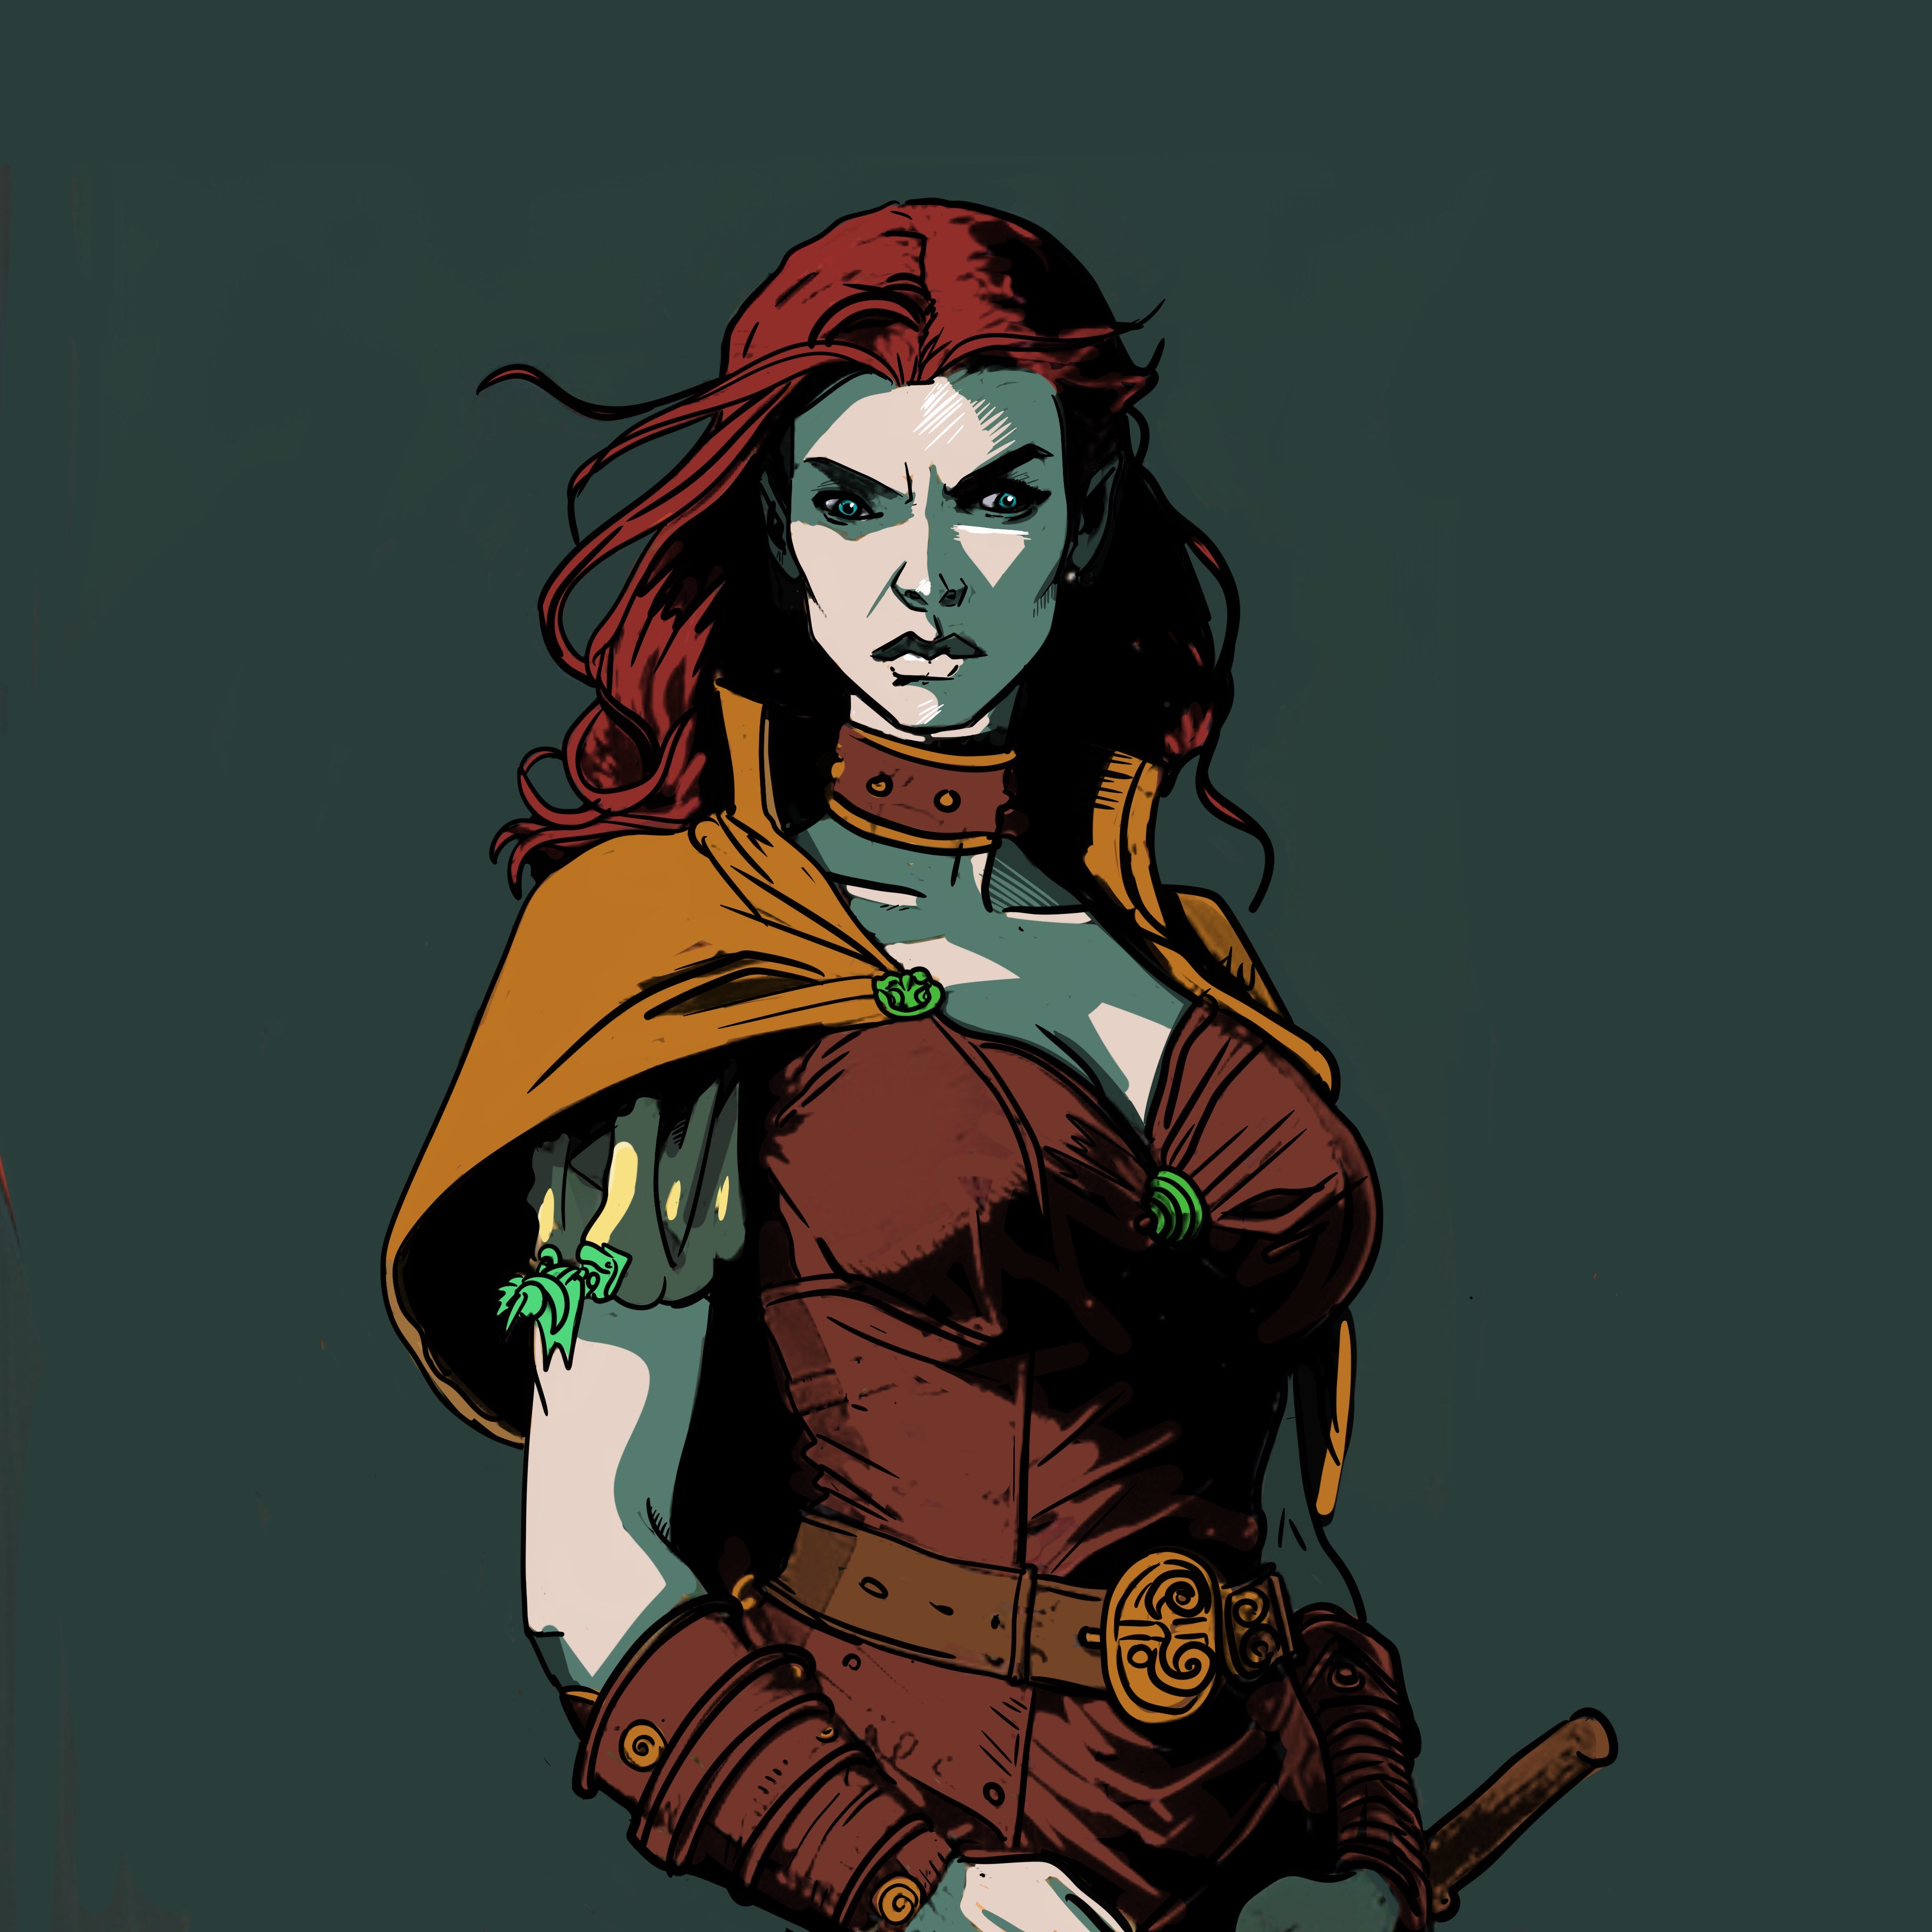
\includegraphics{images/druid.jpg}
\end{center}

\begin{figure*}

\begin{longtable}[]{@{}
  >{\raggedright\arraybackslash}p{(\columnwidth - 28\tabcolsep) * \real{0.0630}}
  >{\raggedleft\arraybackslash}p{(\columnwidth - 28\tabcolsep) * \real{0.1102}}
  >{\centering\arraybackslash}p{(\columnwidth - 28\tabcolsep) * \real{0.0866}}
  >{\centering\arraybackslash}p{(\columnwidth - 28\tabcolsep) * \real{0.0787}}
  >{\centering\arraybackslash}p{(\columnwidth - 28\tabcolsep) * \real{0.0866}}
  >{\centering\arraybackslash}p{(\columnwidth - 28\tabcolsep) * \real{0.0866}}
  >{\raggedright\arraybackslash}p{(\columnwidth - 28\tabcolsep) * \real{0.0315}}
  >{\raggedright\arraybackslash}p{(\columnwidth - 28\tabcolsep) * \real{0.0315}}
  >{\raggedright\arraybackslash}p{(\columnwidth - 28\tabcolsep) * \real{0.0315}}
  >{\raggedright\arraybackslash}p{(\columnwidth - 28\tabcolsep) * \real{0.0315}}
  >{\raggedright\arraybackslash}p{(\columnwidth - 28\tabcolsep) * \real{0.0315}}
  >{\raggedright\arraybackslash}p{(\columnwidth - 28\tabcolsep) * \real{0.0315}}
  >{\raggedright\arraybackslash}p{(\columnwidth - 28\tabcolsep) * \real{0.0315}}
  >{\raggedright\arraybackslash}p{(\columnwidth - 28\tabcolsep) * \real{0.0315}}
  >{\centering\arraybackslash}p{(\columnwidth - 28\tabcolsep) * \real{0.1339}}@{}}
\caption{Druid XP Progression}\label{tbl-xp-druids}\tabularnewline
\toprule\noalign{}
\begin{minipage}[b]{\linewidth}\raggedright
\end{minipage} & \begin{minipage}[b]{\linewidth}\raggedleft
\end{minipage} & \begin{minipage}[b]{\linewidth}\centering
\end{minipage} & \begin{minipage}[b]{\linewidth}\centering
\end{minipage} & \begin{minipage}[b]{\linewidth}\centering
\end{minipage} & \begin{minipage}[b]{\linewidth}\centering
\end{minipage} & \begin{minipage}[b]{\linewidth}\raggedright
\end{minipage} & \begin{minipage}[b]{\linewidth}\raggedright
\end{minipage} &
\multicolumn{4}{>{\raggedright\arraybackslash}p{(\columnwidth - 28\tabcolsep) * \real{0.1260} + 6\tabcolsep}}{%
\begin{minipage}[b]{\linewidth}\raggedright
Spell Level
\end{minipage}} & \begin{minipage}[b]{\linewidth}\raggedright
\end{minipage} & \begin{minipage}[b]{\linewidth}\raggedright
\end{minipage} & \begin{minipage}[b]{\linewidth}\centering
\end{minipage} \\
\begin{minipage}[b]{\linewidth}\raggedright
Level
\end{minipage} & \begin{minipage}[b]{\linewidth}\raggedleft
Exp. Points
\end{minipage} & \begin{minipage}[b]{\linewidth}\centering
Hit Dice
\end{minipage} & \begin{minipage}[b]{\linewidth}\centering
Attack Bonus
\end{minipage} & \begin{minipage}[b]{\linewidth}\centering
Skill Points
\end{minipage} & \begin{minipage}[b]{\linewidth}\centering
Feats
\end{minipage} & \begin{minipage}[b]{\linewidth}\raggedright
0
\end{minipage} & \begin{minipage}[b]{\linewidth}\raggedright
1
\end{minipage} & \begin{minipage}[b]{\linewidth}\raggedright
2
\end{minipage} & \begin{minipage}[b]{\linewidth}\raggedright
3
\end{minipage} & \begin{minipage}[b]{\linewidth}\raggedright
4
\end{minipage} & \begin{minipage}[b]{\linewidth}\raggedright
5
\end{minipage} & \begin{minipage}[b]{\linewidth}\raggedright
6
\end{minipage} & \begin{minipage}[b]{\linewidth}\raggedright
7
\end{minipage} & \begin{minipage}[b]{\linewidth}\centering
Weapon Proficiency
\end{minipage} \\
\midrule\noalign{}
\endfirsthead
\toprule\noalign{}
\begin{minipage}[b]{\linewidth}\raggedright
\end{minipage} & \begin{minipage}[b]{\linewidth}\raggedleft
\end{minipage} & \begin{minipage}[b]{\linewidth}\centering
\end{minipage} & \begin{minipage}[b]{\linewidth}\centering
\end{minipage} & \begin{minipage}[b]{\linewidth}\centering
\end{minipage} & \begin{minipage}[b]{\linewidth}\centering
\end{minipage} & \begin{minipage}[b]{\linewidth}\raggedright
\end{minipage} & \begin{minipage}[b]{\linewidth}\raggedright
\end{minipage} &
\multicolumn{4}{>{\raggedright\arraybackslash}p{(\columnwidth - 28\tabcolsep) * \real{0.1260} + 6\tabcolsep}}{%
\begin{minipage}[b]{\linewidth}\raggedright
Spell Level
\end{minipage}} & \begin{minipage}[b]{\linewidth}\raggedright
\end{minipage} & \begin{minipage}[b]{\linewidth}\raggedright
\end{minipage} & \begin{minipage}[b]{\linewidth}\centering
\end{minipage} \\
\begin{minipage}[b]{\linewidth}\raggedright
Level
\end{minipage} & \begin{minipage}[b]{\linewidth}\raggedleft
Exp. Points
\end{minipage} & \begin{minipage}[b]{\linewidth}\centering
Hit Dice
\end{minipage} & \begin{minipage}[b]{\linewidth}\centering
Attack Bonus
\end{minipage} & \begin{minipage}[b]{\linewidth}\centering
Skill Points
\end{minipage} & \begin{minipage}[b]{\linewidth}\centering
Feats
\end{minipage} & \begin{minipage}[b]{\linewidth}\raggedright
0
\end{minipage} & \begin{minipage}[b]{\linewidth}\raggedright
1
\end{minipage} & \begin{minipage}[b]{\linewidth}\raggedright
2
\end{minipage} & \begin{minipage}[b]{\linewidth}\raggedright
3
\end{minipage} & \begin{minipage}[b]{\linewidth}\raggedright
4
\end{minipage} & \begin{minipage}[b]{\linewidth}\raggedright
5
\end{minipage} & \begin{minipage}[b]{\linewidth}\raggedright
6
\end{minipage} & \begin{minipage}[b]{\linewidth}\raggedright
7
\end{minipage} & \begin{minipage}[b]{\linewidth}\centering
Weapon Proficiency
\end{minipage} \\
\midrule\noalign{}
\endhead
\bottomrule\noalign{}
\endlastfoot
1 & 0 & 1d6 & +1 & 3 & & 1 & -- & -- & -- & -- & -- & -- & -- & 3 \\
2 & 1,500 & 2d6 & +1 & 1 & 1 & 2 & 1 & -- & -- & -- & -- & -- & -- & \\
3 & 3,000 & 3d6 & +1 & 1 & & 3 & 2 & -- & -- & -- & -- & -- & -- & \\
4 & 6,000 & 4d6 & +2 & 1 & 1 & 4 & 2 & 1 & -- & -- & -- & -- & -- & \\
5 & 12,000 & 5d6 & +2 & 1 & & 5 & 2 & 2 & -- & -- & -- & -- & -- & 1 \\
6 & 24,000 & 6d6 & +3 & 1 & 1 & 6 & 2 & 2 & 1 & -- & -- & -- & -- & \\
7 & 48,000 & 7d6 & +3 & 1 & & 7 & 3 & 2 & 2 & -- & -- & -- & -- & \\
8 & 90,000 & 8d6 & +3 & 1 & 1 & 8 & 3 & 2 & 2 & 1 & -- & -- & -- & \\
9 & 180,000 & 9d6 & +4 & 1 & & 9 & 3 & 3 & 2 & 2 & -- & -- & -- & 1 \\
10 & 270,000 & 9d6+1 & +4 & 1 & 1 & 9 & 3 & 3 & 2 & 2 & 1 & -- & -- & \\
11 & 360,000 & 9d6+2 & +4 & 1 & & 9 & 4 & 3 & 3 & 2 & 2 & -- & -- & \\
12 & 450,000 & 9d6+3 & +4 & 1 & 1 & 9 & 4 & 4 & 3 & 2 & 2 & 1 & -- & \\
13 & 540,000 & 9d6+4 & +5 & 1 & & 9 & 4 & 4 & 3 & 3 & 2 & 2 & -- & 1 \\
14 & 630,000 & 9d6+5 & +5 & 1 & 1 & 9 & 4 & 4 & 4 & 3 & 2 & 2 & 1 & \\
15 & 720,000 & 9d6+6 & +5 & 1 & & 9 & 4 & 4 & 4 & 3 & 3 & 2 & 1 & \\
16 & 810,000 & 9d6+7 & +6 & 1 & 1 & 9 & 5 & 4 & 4 & 3 & 3 & 2 & 1 & \\
17 & 900,000 & 9d6+8 & +6 & 1 & & 9 & 5 & 5 & 4 & 3 & 3 & 2 & 2 & 1 \\
18 & 990,000 & 9d6+9 & +6 & 1 & 1 & 9 & 5 & 5 & 4 & 4 & 3 & 3 & 2 & \\
19 & 1,080,000 & 9d6+10 & +7 & 1 & & 9 & 6 & 5 & 4 & 4 & 3 & 3 & 2 & \\
20 & 1,170,000 & 9d6+11 & +7 & 1 & 1 & 9 & 6 & 5 & 4 & 4 & 3 & 3 & 3
& \\
\end{longtable}

\end{figure*}%

\begin{longtable}[]{@{}ll@{}}
\caption{Druid Wisdom Bonus}\label{tbl-wisdom-druids}\tabularnewline
\toprule\noalign{}
Wisdom & Spell Bonus \\
\midrule\noalign{}
\endfirsthead
\toprule\noalign{}
Wisdom & Spell Bonus \\
\midrule\noalign{}
\endhead
\bottomrule\noalign{}
\endlastfoot
9-11 & No bonus spells \\
12 & +1 Orison \\
13-15 & +1 Orison, +1 1\textsuperscript{st} level spell \\
16-17 & +2 Orisons, +2 1\textsuperscript{st} level spells \\
18 & +3 Orisons, +3 1\textsuperscript{st} level, +1
2\textsuperscript{nd} level spells \\
\end{longtable}

\begin{longtable}[]{@{}
  >{\raggedright\arraybackslash}p{(\columnwidth - 16\tabcolsep) * \real{0.1300}}
  >{\raggedright\arraybackslash}p{(\columnwidth - 16\tabcolsep) * \real{0.1000}}
  >{\raggedright\arraybackslash}p{(\columnwidth - 16\tabcolsep) * \real{0.1000}}
  >{\raggedright\arraybackslash}p{(\columnwidth - 16\tabcolsep) * \real{0.1000}}
  >{\raggedright\arraybackslash}p{(\columnwidth - 16\tabcolsep) * \real{0.1300}}
  >{\raggedright\arraybackslash}p{(\columnwidth - 16\tabcolsep) * \real{0.0800}}
  >{\raggedright\arraybackslash}p{(\columnwidth - 16\tabcolsep) * \real{0.0800}}
  >{\raggedright\arraybackslash}p{(\columnwidth - 16\tabcolsep) * \real{0.1500}}
  >{\raggedright\arraybackslash}p{(\columnwidth - 16\tabcolsep) * \real{0.1300}}@{}}
\caption{Druid Titles}\label{tbl-titles-druids}\tabularnewline
\toprule\noalign{}
\begin{minipage}[b]{\linewidth}\raggedright
Druid Level
\end{minipage} & \begin{minipage}[b]{\linewidth}\raggedright
1\textsuperscript{st}
\end{minipage} & \begin{minipage}[b]{\linewidth}\raggedright
2\textsuperscript{nd}
\end{minipage} & \begin{minipage}[b]{\linewidth}\raggedright
3\textsuperscript{rd}
\end{minipage} & \begin{minipage}[b]{\linewidth}\raggedright
4\textsuperscript{th}
\end{minipage} & \begin{minipage}[b]{\linewidth}\raggedright
5\textsuperscript{th}
\end{minipage} & \begin{minipage}[b]{\linewidth}\raggedright
9\textsuperscript{th}
\end{minipage} & \begin{minipage}[b]{\linewidth}\raggedright
12\textsuperscript{th}
\end{minipage} & \begin{minipage}[b]{\linewidth}\raggedright
15\textsuperscript{th}
\end{minipage} \\
\midrule\noalign{}
\endfirsthead
\toprule\noalign{}
\begin{minipage}[b]{\linewidth}\raggedright
Druid Level
\end{minipage} & \begin{minipage}[b]{\linewidth}\raggedright
1\textsuperscript{st}
\end{minipage} & \begin{minipage}[b]{\linewidth}\raggedright
2\textsuperscript{nd}
\end{minipage} & \begin{minipage}[b]{\linewidth}\raggedright
3\textsuperscript{rd}
\end{minipage} & \begin{minipage}[b]{\linewidth}\raggedright
4\textsuperscript{th}
\end{minipage} & \begin{minipage}[b]{\linewidth}\raggedright
5\textsuperscript{th}
\end{minipage} & \begin{minipage}[b]{\linewidth}\raggedright
9\textsuperscript{th}
\end{minipage} & \begin{minipage}[b]{\linewidth}\raggedright
12\textsuperscript{th}
\end{minipage} & \begin{minipage}[b]{\linewidth}\raggedright
15\textsuperscript{th}
\end{minipage} \\
\midrule\noalign{}
\endhead
\bottomrule\noalign{}
\endlastfoot
Rank/Title & Aspirant & Initiate & Wayfarer & Grovekeeper & Warden &
Herald & Spring Walker & Elder Druid \\
\end{longtable}

\begin{longtable}[]{@{}
  >{\raggedright\arraybackslash}p{(\columnwidth - 10\tabcolsep) * \real{0.1250}}
  >{\raggedright\arraybackslash}p{(\columnwidth - 10\tabcolsep) * \real{0.2273}}
  >{\raggedright\arraybackslash}p{(\columnwidth - 10\tabcolsep) * \real{0.1477}}
  >{\raggedright\arraybackslash}p{(\columnwidth - 10\tabcolsep) * \real{0.2386}}
  >{\raggedright\arraybackslash}p{(\columnwidth - 10\tabcolsep) * \real{0.1705}}
  >{\raggedright\arraybackslash}p{(\columnwidth - 10\tabcolsep) * \real{0.0909}}@{}}
\caption{Druid Saving Throws}\label{tbl-save-druids}\tabularnewline
\toprule\noalign{}
\begin{minipage}[b]{\linewidth}\raggedright
\textbf{Level}
\end{minipage} & \begin{minipage}[b]{\linewidth}\raggedright
Death Ray / Poison
\end{minipage} & \begin{minipage}[b]{\linewidth}\raggedright
Magic Wands
\end{minipage} & \begin{minipage}[b]{\linewidth}\raggedright
Paralysis / Petrify
\end{minipage} & \begin{minipage}[b]{\linewidth}\raggedright
Dragon Breath
\end{minipage} & \begin{minipage}[b]{\linewidth}\raggedright
Spells
\end{minipage} \\
\midrule\noalign{}
\endfirsthead
\toprule\noalign{}
\begin{minipage}[b]{\linewidth}\raggedright
\textbf{Level}
\end{minipage} & \begin{minipage}[b]{\linewidth}\raggedright
Death Ray / Poison
\end{minipage} & \begin{minipage}[b]{\linewidth}\raggedright
Magic Wands
\end{minipage} & \begin{minipage}[b]{\linewidth}\raggedright
Paralysis / Petrify
\end{minipage} & \begin{minipage}[b]{\linewidth}\raggedright
Dragon Breath
\end{minipage} & \begin{minipage}[b]{\linewidth}\raggedright
Spells
\end{minipage} \\
\midrule\noalign{}
\endhead
\bottomrule\noalign{}
\endlastfoot
\textbf{1} & 13 & 14 & 13 & 16 & 15 \\
\textbf{2-3} & 13 & 14 & 13 & 15 & 14 \\
\textbf{4-5} & 12 & 13 & 12 & 15 & 13 \\
\textbf{6-7} & 12 & 12 & 11 & 14 & 13 \\
\textbf{8-9} & 11 & 11 & 10 & 14 & 12 \\
\textbf{10-11} & 11 & 10 & 9 & 13 & 11 \\
\textbf{12-13} & 10 & 10 & 9 & 13 & 11 \\
\textbf{14-15} & 10 & 9 & 8 & 12 & 10 \\
\textbf{16-17} & 9 & 8 & 7 & 12 & 9 \\
\textbf{18-19} & 9 & 7 & 6 & 11 & 9 \\
\textbf{20} & 8 & 6 & 5 & 11 & 8 \\
\end{longtable}

\subsection{Animal Affinity}\label{animal-affinity}

Druids can calm or befriend animals. The Druid rolls a d20 and adds
their Wisdom Bonus. Cross-reference the Druid's level with the animal's
hit dice on the Druids Animal Affinity Table. The number shown is the
minimum needed to Calm that sort of animal.~ Tame, Domesticated, or
Normal Beasts of Burden are treated as half their actual Hit Dice,
reflecting their relatively easy manageability. Monstrous animals such
as griffins, owlbears, pegasi, or other such ``near-natural'' creatures
are treated as they are 1 HD more than listed to reflect their unique
natures.~

If the table indicates ``No'' then it is not possible for the Druid to
affect that type of animal. If the table says ``C'' for that
combination, that type of animal is automatically calmed. If the result
shown is a ``B'' for that combination, that type of animal is
automatically befriended. If the roll is a success, 2d6 HD of animals is
affected. Surplus hit dice are lost, but at least one animal is always
affected if the first roll is a success.~ If a mixed group of animals is
to be affected, the druid rolls just once. The result is checked against
the weakest sort first and if they are successfully Calmed or
Befriended, the same result is checked against the next higher type of
animal.

If a Druid succeeds at Calming or Befriending some of the animals, but
not all are affected, they may try again in the next round to affect
those which remain. If any roll to Calm or Befriend the Animals fails,
that Druid may not attempt to use their Animal Affinity ability again
for one full turn. A partial failure (possible against a mixed group)
counts as a failure for this purpose.

Calm animals will not interact with the Druid in any manner, unless
approached by the Druid. The Druid can calmly get them to leave an area,
or the Druid can try to befriend the animals. In this case, the DM
should roll a \hyperref[tbl-monsterReactions]{reaction roll} with any
result below ``uncertain'' meaning the animals flee. If the result on
the table results in automatically befriending the animals, the DM
should treat the animals as if a ``Friendly,'' result was rolled on the
Reaction Roll Table. A Befriended animal will follow the Druid, guarding
and assisting within its capabilities so long as the Druid remains in
the general vicinity of its normal lair or range. However, it will not
fight to the death or sacrifice itself indiscriminately. When
substantially wounded, an animal will flee the area immediately. The DM
may \hyperref[morale]{check morale} as necessary when the situation
seems appropriate.

\begin{figure*}

\begin{longtable}[]{@{}
  >{\raggedright\arraybackslash}p{(\columnwidth - 22\tabcolsep) * \real{0.1358}}
  >{\raggedright\arraybackslash}p{(\columnwidth - 22\tabcolsep) * \real{0.1111}}
  >{\raggedright\arraybackslash}p{(\columnwidth - 22\tabcolsep) * \real{0.0741}}
  >{\raggedright\arraybackslash}p{(\columnwidth - 22\tabcolsep) * \real{0.0741}}
  >{\raggedright\arraybackslash}p{(\columnwidth - 22\tabcolsep) * \real{0.0741}}
  >{\raggedright\arraybackslash}p{(\columnwidth - 22\tabcolsep) * \real{0.0741}}
  >{\raggedright\arraybackslash}p{(\columnwidth - 22\tabcolsep) * \real{0.0741}}
  >{\raggedright\arraybackslash}p{(\columnwidth - 22\tabcolsep) * \real{0.0741}}
  >{\raggedright\arraybackslash}p{(\columnwidth - 22\tabcolsep) * \real{0.0741}}
  >{\raggedright\arraybackslash}p{(\columnwidth - 22\tabcolsep) * \real{0.0741}}
  >{\raggedright\arraybackslash}p{(\columnwidth - 22\tabcolsep) * \real{0.0741}}
  >{\raggedright\arraybackslash}p{(\columnwidth - 22\tabcolsep) * \real{0.0864}}@{}}
\caption{Druid Animal Affinity}\label{tbl-animal-druids}\tabularnewline
\toprule\noalign{}
\begin{minipage}[b]{\linewidth}\raggedright
Druid Lvl
\end{minipage} & \begin{minipage}[b]{\linewidth}\raggedright
\textless{} 1 HD
\end{minipage} & \begin{minipage}[b]{\linewidth}\raggedright
1 HD
\end{minipage} & \begin{minipage}[b]{\linewidth}\raggedright
2 HD
\end{minipage} & \begin{minipage}[b]{\linewidth}\raggedright
3 HD
\end{minipage} & \begin{minipage}[b]{\linewidth}\raggedright
4 HD
\end{minipage} & \begin{minipage}[b]{\linewidth}\raggedright
5 HD
\end{minipage} & \begin{minipage}[b]{\linewidth}\raggedright
6 HD
\end{minipage} & \begin{minipage}[b]{\linewidth}\raggedright
7 HD
\end{minipage} & \begin{minipage}[b]{\linewidth}\raggedright
8 HD
\end{minipage} & \begin{minipage}[b]{\linewidth}\raggedright
9 HD
\end{minipage} & \begin{minipage}[b]{\linewidth}\raggedright
10 HD
\end{minipage} \\
\midrule\noalign{}
\endfirsthead
\toprule\noalign{}
\begin{minipage}[b]{\linewidth}\raggedright
Druid Lvl
\end{minipage} & \begin{minipage}[b]{\linewidth}\raggedright
\textless{} 1 HD
\end{minipage} & \begin{minipage}[b]{\linewidth}\raggedright
1 HD
\end{minipage} & \begin{minipage}[b]{\linewidth}\raggedright
2 HD
\end{minipage} & \begin{minipage}[b]{\linewidth}\raggedright
3 HD
\end{minipage} & \begin{minipage}[b]{\linewidth}\raggedright
4 HD
\end{minipage} & \begin{minipage}[b]{\linewidth}\raggedright
5 HD
\end{minipage} & \begin{minipage}[b]{\linewidth}\raggedright
6 HD
\end{minipage} & \begin{minipage}[b]{\linewidth}\raggedright
7 HD
\end{minipage} & \begin{minipage}[b]{\linewidth}\raggedright
8 HD
\end{minipage} & \begin{minipage}[b]{\linewidth}\raggedright
9 HD
\end{minipage} & \begin{minipage}[b]{\linewidth}\raggedright
10 HD
\end{minipage} \\
\midrule\noalign{}
\endhead
\bottomrule\noalign{}
\endlastfoot
1 & 9 & 13 & 17 & 19 & No & No & No & No & No & No & No \\
2 & 7 & 11 & 15 & 18 & 20 & No & No & No & No & No & No \\
3 & 5 & 9 & 13 & 17 & 19 & No & No & No & No & No & No \\
4 & 3 & 7 & 11 & 15 & 18 & 20 & No & No & No & No & No \\
5 & 2 & 5 & 9 & 13 & 17 & 19 & No & No & No & No & No \\
6 & C & 3 & 7 & 11 & 15 & 18 & 20 & No & No & No & No \\
7 & C & 2 & 5 & 9 & 13 & 17 & 19 & No & No & No & No \\
8 & C & C & 3 & 7 & 11 & 15 & 18 & 20 & No & No & No \\
9 & B & C & 2 & 5 & 9 & 13 & 17 & 19 & No & No & No \\
10 & B & C & C & 3 & 7 & 11 & 15 & 18 & 20 & No & No \\
11 & B & B & C & 2 & 5 & 9 & 13 & 17 & 19 & No & No \\
12 & B & B & C & C & 3 & 7 & 11 & 15 & 18 & 20 & No \\
13 & B & B & B & C & 2 & 5 & 9 & 13 & 17 & 19 & No \\
14 & B & B & B & C & C & 3 & 7 & 11 & 15 & 18 & 20 \\
15 & B & B & B & B & C & 2 & 5 & 9 & 13 & 17 & 19 \\
16 & B & B & B & B & C & C & 3 & 7 & 11 & 15 & 18 \\
17 & B & B & B & B & B & C & 2 & 5 & 9 & 13 & 17 \\
18 & B & B & B & B & B & C & C & 3 & 7 & 11 & 15 \\
19 & B & B & B & B & B & B & C & 2 & 5 & 9 & 13 \\
20 & B & B & B & B & B & B & C & C & 3 & 7 & 11 \\
\end{longtable}

\end{figure*}%

\section{Fighter}\label{fighter}

\begin{center}

\includegraphics{images/fighter_class.png}
\end{center}

Fighters include soldiers, town guardsmen, barbarian warriors, and
anyone else for whom fighting is a way of life. They train in combat,
and they generally approach problems head on, weapon drawn. Not
surprisingly, Fighters are the best at fighting of all the classes. They
are also the hardiest, able to take more punishment than any other
class.

The Prime Requisite for Fighters is Strength; a character must have a
Strength score of 9 or higher to become a Fighter. Members of this class
may wear any armor and use any weapon.

\begin{center}
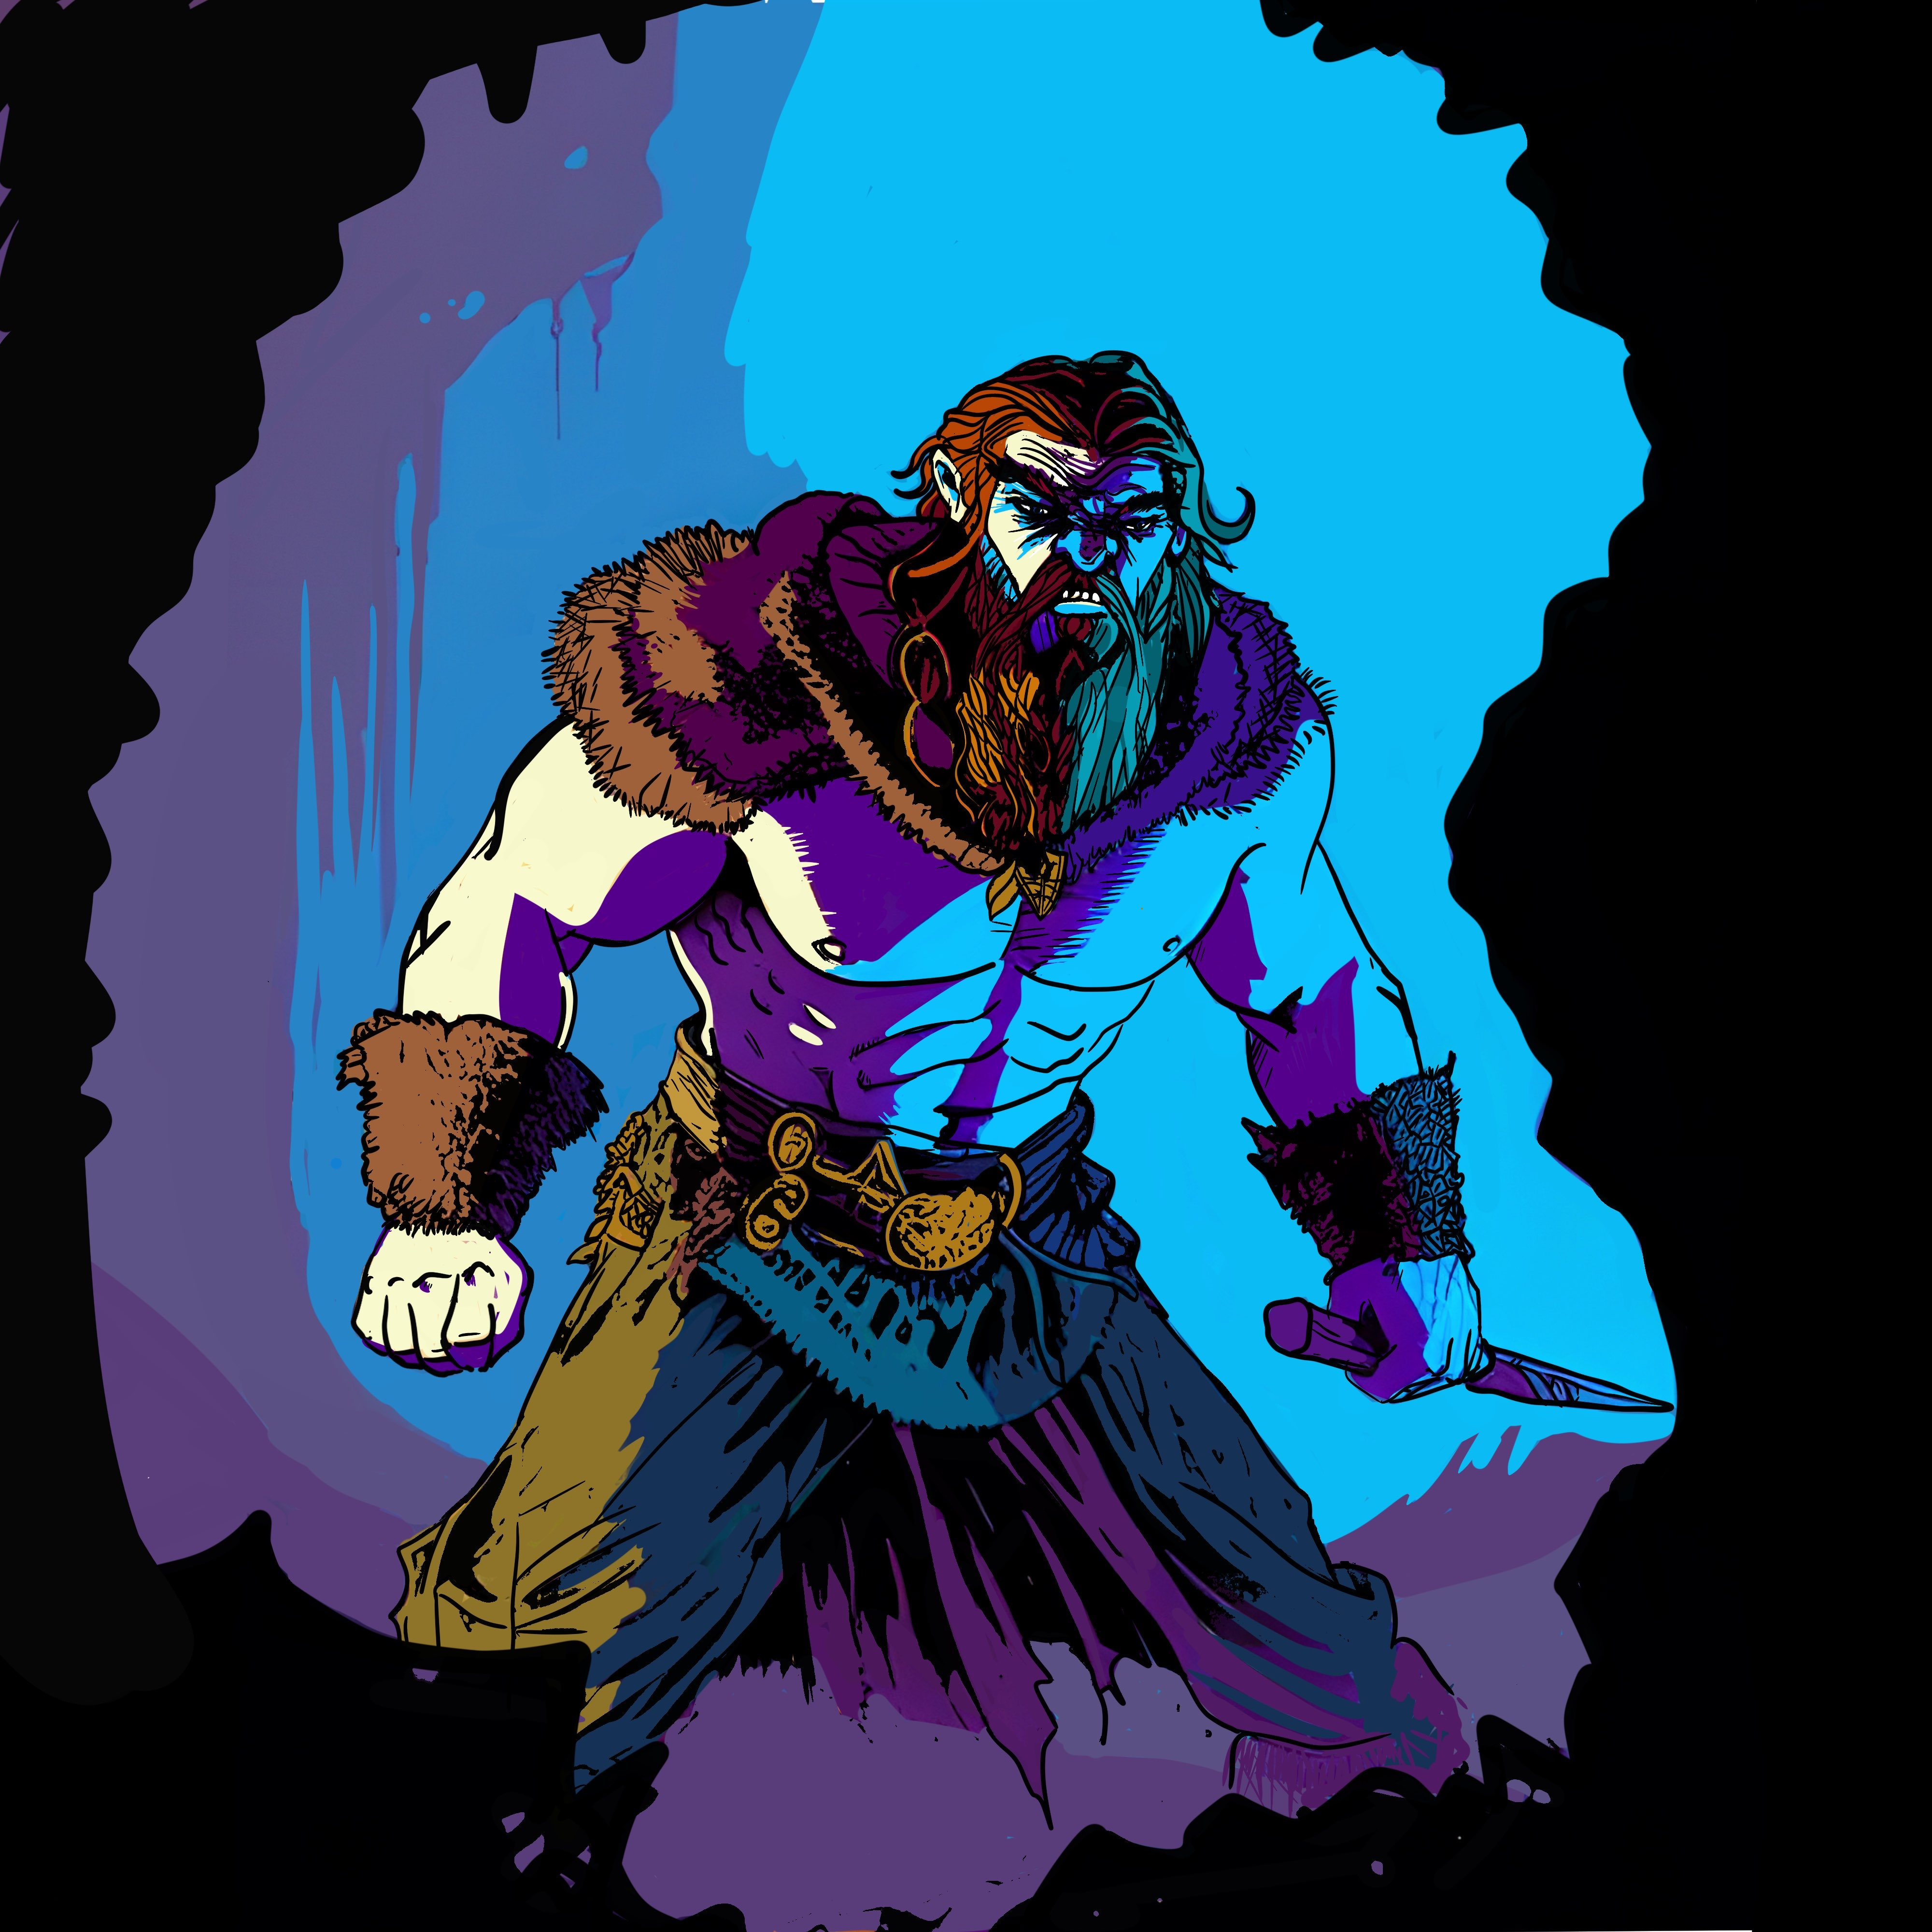
\includegraphics{images/fighter.jpg}
\end{center}

\begin{figure*}

\begin{longtable}[]{@{}
  >{\raggedright\arraybackslash}p{(\columnwidth - 16\tabcolsep) * \real{0.0551}}
  >{\raggedright\arraybackslash}p{(\columnwidth - 16\tabcolsep) * \real{0.1024}}
  >{\raggedright\arraybackslash}p{(\columnwidth - 16\tabcolsep) * \real{0.0787}}
  >{\raggedright\arraybackslash}p{(\columnwidth - 16\tabcolsep) * \real{0.1102}}
  >{\raggedright\arraybackslash}p{(\columnwidth - 16\tabcolsep) * \real{0.1496}}
  >{\raggedright\arraybackslash}p{(\columnwidth - 16\tabcolsep) * \real{0.1811}}
  >{\raggedright\arraybackslash}p{(\columnwidth - 16\tabcolsep) * \real{0.1102}}
  >{\raggedright\arraybackslash}p{(\columnwidth - 16\tabcolsep) * \real{0.0551}}
  >{\raggedright\arraybackslash}p{(\columnwidth - 16\tabcolsep) * \real{0.1575}}@{}}
\caption{Fighter XP Progression}\label{tbl-xp-fighters}\tabularnewline
\toprule\noalign{}
\begin{minipage}[b]{\linewidth}\raggedright
Level
\end{minipage} & \begin{minipage}[b]{\linewidth}\raggedright
Exp. Points
\end{minipage} & \begin{minipage}[b]{\linewidth}\raggedright
Hit Dice
\end{minipage} & \begin{minipage}[b]{\linewidth}\raggedright
Attack Bonus
\end{minipage} & \begin{minipage}[b]{\linewidth}\raggedright
Attacks/Round
\end{minipage} & \begin{minipage}[b]{\linewidth}\raggedright
Weapon Specialization
\end{minipage} & \begin{minipage}[b]{\linewidth}\raggedright
Skill points
\end{minipage} & \begin{minipage}[b]{\linewidth}\raggedright
Feats
\end{minipage} & \begin{minipage}[b]{\linewidth}\raggedright
Weapon Proficiency
\end{minipage} \\
\midrule\noalign{}
\endfirsthead
\toprule\noalign{}
\begin{minipage}[b]{\linewidth}\raggedright
Level
\end{minipage} & \begin{minipage}[b]{\linewidth}\raggedright
Exp. Points
\end{minipage} & \begin{minipage}[b]{\linewidth}\raggedright
Hit Dice
\end{minipage} & \begin{minipage}[b]{\linewidth}\raggedright
Attack Bonus
\end{minipage} & \begin{minipage}[b]{\linewidth}\raggedright
Attacks/Round
\end{minipage} & \begin{minipage}[b]{\linewidth}\raggedright
Weapon Specialization
\end{minipage} & \begin{minipage}[b]{\linewidth}\raggedright
Skill points
\end{minipage} & \begin{minipage}[b]{\linewidth}\raggedright
Feats
\end{minipage} & \begin{minipage}[b]{\linewidth}\raggedright
Weapon Proficiency
\end{minipage} \\
\midrule\noalign{}
\endhead
\bottomrule\noalign{}
\endlastfoot
1 & 0 & 1d10 & +1 & 1/1 & +1/+0 & 3 & & 4 \\
2 & 2,000 & 2d10 & +2 & 1/1 & +1/+0 & 1 & 1 & \\
3 & 4,000 & 3d10 & +2 & 1/1 & +1/+0 & 1 & & 1 \\
4 & 8,000 & 4d10 & +3 & 1/1 & +1/+1 & 1 & 1 & \\
5 & 16,000 & 5d10 & +4 & 1/1 & +1/+1 & 1 & & 1 \\
6 & 32,000 & 6d10 & +4 & 1/1 & +1/+1 & 1 & 1 & \\
7 & 64,000 & 7d10 & +5 & 3/2 & +2/+1 & 1 & & 1 \\
8 & 120,000 & 8d10 & +6 & 3/2 & +2/+2 & 1 & 1 & \\
9 & 240,000 & 9d10 & +6 & 3/2 & +2/+2 & 1 & & 1 \\
10 & 360,000 & 9d10+2 & +6 & 3/2 & +2/+2 & 1 & 1 & \\
11 & 480,000 & 9d10+4 & +7 & 3/2 & +2/+2 & 1 & & 1 \\
12 & 600,000 & 9d10+6 & +7 & 3/2 & +2/+2 & 1 & 1 & \\
13 & 720,000 & 9d10+8 & +8 & 2/1 & +3/+2 & 1 & & 1 \\
14 & 840,000 & 9d10+10 & +8 & 2/1 & +3/+2 & 1 & 1 & \\
15 & 960,000 & 9d10+12 & +8 & 2/1 & +3/+2 & 1 & & 1 \\
16 & 1,080,000 & 9d10+14 & +9 & 2/1 & +3/+3 & 1 & 1 & \\
17 & 1,200,000 & 9d10+16 & +9 & 2/1 & +3/+3 & 1 & & 1 \\
18 & 1,320,000 & 9d10+18 & +10 & 3/1 & +3/+3 & 1 & 1 & \\
19 & 1,440,000 & 9d10+20 & +10 & 3/1 & +3/+3 & 1 & & 1 \\
20 & 1,560,000 & 9d10+22 & +10 & 3/1 & +3/+3 & 1 & 1 & \\
\end{longtable}

\end{figure*}%

\begin{longtable}[]{@{}ll@{}}
\caption{Fighter Attack Bonus}\label{tbl-bonus-fighters}\tabularnewline
\toprule\noalign{}
Strength & Fighting Bonus \\
\midrule\noalign{}
\endfirsthead
\toprule\noalign{}
Strength & Fighting Bonus \\
\midrule\noalign{}
\endhead
\bottomrule\noalign{}
\endlastfoot
9-12 & +0 to hit, +0 damage \\
13-15 & +1 to hit, +1 damage \\
16-17 & +2 to hit, +2 damage \\
18 & +3 to hit, +3 damage \\
\end{longtable}

\begin{figure*}

\begin{longtable}[]{@{}
  >{\raggedright\arraybackslash}p{(\columnwidth - 16\tabcolsep) * \real{0.0833}}
  >{\raggedright\arraybackslash}p{(\columnwidth - 16\tabcolsep) * \real{0.0833}}
  >{\raggedright\arraybackslash}p{(\columnwidth - 16\tabcolsep) * \real{0.0833}}
  >{\raggedright\arraybackslash}p{(\columnwidth - 16\tabcolsep) * \real{0.0833}}
  >{\raggedright\arraybackslash}p{(\columnwidth - 16\tabcolsep) * \real{0.1136}}
  >{\raggedright\arraybackslash}p{(\columnwidth - 16\tabcolsep) * \real{0.1136}}
  >{\raggedright\arraybackslash}p{(\columnwidth - 16\tabcolsep) * \real{0.1364}}
  >{\raggedright\arraybackslash}p{(\columnwidth - 16\tabcolsep) * \real{0.1288}}
  >{\raggedright\arraybackslash}p{(\columnwidth - 16\tabcolsep) * \real{0.1742}}@{}}
\caption{Fighter Titles}\label{tbl-titles-figthers}\tabularnewline
\toprule\noalign{}
\begin{minipage}[b]{\linewidth}\raggedright
Alignment
\end{minipage} & \begin{minipage}[b]{\linewidth}\raggedright
Level 1
\end{minipage} & \begin{minipage}[b]{\linewidth}\raggedright
Level 2
\end{minipage} & \begin{minipage}[b]{\linewidth}\raggedright
Level 3
\end{minipage} & \begin{minipage}[b]{\linewidth}\raggedright
Level 4
\end{minipage} & \begin{minipage}[b]{\linewidth}\raggedright
Level 5
\end{minipage} & \begin{minipage}[b]{\linewidth}\raggedright
Level 9
\end{minipage} & \begin{minipage}[b]{\linewidth}\raggedright
Level 12
\end{minipage} & \begin{minipage}[b]{\linewidth}\raggedright
Level 15
\end{minipage} \\
\midrule\noalign{}
\endfirsthead
\toprule\noalign{}
\begin{minipage}[b]{\linewidth}\raggedright
Alignment
\end{minipage} & \begin{minipage}[b]{\linewidth}\raggedright
Level 1
\end{minipage} & \begin{minipage}[b]{\linewidth}\raggedright
Level 2
\end{minipage} & \begin{minipage}[b]{\linewidth}\raggedright
Level 3
\end{minipage} & \begin{minipage}[b]{\linewidth}\raggedright
Level 4
\end{minipage} & \begin{minipage}[b]{\linewidth}\raggedright
Level 5
\end{minipage} & \begin{minipage}[b]{\linewidth}\raggedright
Level 9
\end{minipage} & \begin{minipage}[b]{\linewidth}\raggedright
Level 12
\end{minipage} & \begin{minipage}[b]{\linewidth}\raggedright
Level 15
\end{minipage} \\
\midrule\noalign{}
\endhead
\bottomrule\noalign{}
\endlastfoot
Lawful & Squire & Sergeant & Cavalier & Knight & Captain & Commander &
Thane & Lord/Lady \\
Neutral & Bravo & Duelist & Sellsword & Swordsmen & Swordsmaster &
Vangaurd & Warchief & Chieftain \\
Chaotic & Brawler & Raider & Marauder & Ravager & Reaver & Warmonger &
Warlord & Overlord \\
\end{longtable}

\end{figure*}%

\begin{longtable}[]{@{}
  >{\raggedright\arraybackslash}p{(\columnwidth - 10\tabcolsep) * \real{0.1250}}
  >{\raggedright\arraybackslash}p{(\columnwidth - 10\tabcolsep) * \real{0.2273}}
  >{\raggedright\arraybackslash}p{(\columnwidth - 10\tabcolsep) * \real{0.1477}}
  >{\raggedright\arraybackslash}p{(\columnwidth - 10\tabcolsep) * \real{0.2386}}
  >{\raggedright\arraybackslash}p{(\columnwidth - 10\tabcolsep) * \real{0.1705}}
  >{\raggedright\arraybackslash}p{(\columnwidth - 10\tabcolsep) * \real{0.0909}}@{}}
\caption{Fighter Saving Throws}\label{tbl-save-fighter}\tabularnewline
\toprule\noalign{}
\begin{minipage}[b]{\linewidth}\raggedright
\textbf{Level}
\end{minipage} & \begin{minipage}[b]{\linewidth}\raggedright
Death Ray / Poison
\end{minipage} & \begin{minipage}[b]{\linewidth}\raggedright
Magic Wands
\end{minipage} & \begin{minipage}[b]{\linewidth}\raggedright
Paralysis / Petrify
\end{minipage} & \begin{minipage}[b]{\linewidth}\raggedright
Dragon Breath
\end{minipage} & \begin{minipage}[b]{\linewidth}\raggedright
Spells
\end{minipage} \\
\midrule\noalign{}
\endfirsthead
\toprule\noalign{}
\begin{minipage}[b]{\linewidth}\raggedright
\textbf{Level}
\end{minipage} & \begin{minipage}[b]{\linewidth}\raggedright
Death Ray / Poison
\end{minipage} & \begin{minipage}[b]{\linewidth}\raggedright
Magic Wands
\end{minipage} & \begin{minipage}[b]{\linewidth}\raggedright
Paralysis / Petrify
\end{minipage} & \begin{minipage}[b]{\linewidth}\raggedright
Dragon Breath
\end{minipage} & \begin{minipage}[b]{\linewidth}\raggedright
Spells
\end{minipage} \\
\midrule\noalign{}
\endhead
\bottomrule\noalign{}
\endlastfoot
\textbf{NM} & 13 & 14 & 15 & 16 & 18 \\
\textbf{1} & 12 & 13 & 14 & 15 & 17 \\
\textbf{2-3} & 11 & 12 & 14 & 15 & 16 \\
\textbf{4-5} & 11 & 11 & 13 & 14 & 15 \\
\textbf{6-7} & 10 & 11 & 12 & 14 & 15 \\
\textbf{8-9} & 9 & 10 & 12 & 13 & 14 \\
\textbf{10-11} & 9 & 9 & 11 & 12 & 13 \\
\textbf{12-13} & 8 & 9 & 10 & 12 & 13 \\
\textbf{14-15} & 7 & 8 & 10 & 11 & 12 \\
\textbf{16-17} & 7 & 7 & 9 & 10 & 11 \\
\textbf{18-19} & 6 & 7 & 8 & 10 & 11 \\
\textbf{20} & 5 & 6 & 8 & 9 & 10 \\
\end{longtable}

\subsection{Weapon Specialization}\label{weapon-specialization}

A Fighter chooses one weapon in which the character is especially
skilled. This choice must be specific; for instance, a specialization in
the longsword will give no bonuses when using a shortsword. The weapon
specialization confers additional to hit and damage bonuses as the
fighter progresses in rank.

Paladins and Rangers cannot specialize.

\section{Paladin}\label{paladin}

\begin{center}

\includegraphics[width=2.08333in,height=\textheight]{images/paladin_class.png}
\end{center}

Paladins are the epitome of honor, courage, and righteousness, standing
as beacons of hope against the growing darkness descending over the
OnceWas. They are holy warriors, dedicated to upholding the tenets of
justice and vanquishing evil wherever it may lurk. Blessed by divine
powers, Paladins serve as champions of the gods, drawing upon their
faith to perform miraculous feats and protect the innocent.

A character must a minimum Strength score of 9, a Wisdom score of 11,
and a Charisma score of 11 to be a Paladin. Paladins must be human or
half-even. They may use any weapon and may wear any armor or shield.

Paladins have the same attack bonus and saving throws as Fighters of the
same level. They should be treated as Fighters for all purposes except
they may not specialize.

\begin{figure*}

\begin{longtable}[]{@{}
  >{\raggedright\arraybackslash}p{(\columnwidth - 22\tabcolsep) * \real{0.0672}}
  >{\raggedleft\arraybackslash}p{(\columnwidth - 22\tabcolsep) * \real{0.1176}}
  >{\centering\arraybackslash}p{(\columnwidth - 22\tabcolsep) * \real{0.0924}}
  >{\centering\arraybackslash}p{(\columnwidth - 22\tabcolsep) * \real{0.0840}}
  >{\centering\arraybackslash}p{(\columnwidth - 22\tabcolsep) * \real{0.1092}}
  >{\centering\arraybackslash}p{(\columnwidth - 22\tabcolsep) * \real{0.0924}}
  >{\centering\arraybackslash}p{(\columnwidth - 22\tabcolsep) * \real{0.0924}}
  >{\raggedright\arraybackslash}p{(\columnwidth - 22\tabcolsep) * \real{0.0336}}
  >{\raggedright\arraybackslash}p{(\columnwidth - 22\tabcolsep) * \real{0.0336}}
  >{\raggedright\arraybackslash}p{(\columnwidth - 22\tabcolsep) * \real{0.0336}}
  >{\raggedright\arraybackslash}p{(\columnwidth - 22\tabcolsep) * \real{0.0336}}
  >{\centering\arraybackslash}p{(\columnwidth - 22\tabcolsep) * \real{0.1261}}@{}}
\caption{Paladin XP Progression}\label{tbl-xp-paladin}\tabularnewline
\toprule\noalign{}
\begin{minipage}[b]{\linewidth}\raggedright
\end{minipage} & \begin{minipage}[b]{\linewidth}\raggedleft
\end{minipage} & \begin{minipage}[b]{\linewidth}\centering
\end{minipage} & \begin{minipage}[b]{\linewidth}\centering
\end{minipage} & \begin{minipage}[b]{\linewidth}\centering
\end{minipage} & \begin{minipage}[b]{\linewidth}\centering
\end{minipage} & \begin{minipage}[b]{\linewidth}\centering
\end{minipage} &
\multicolumn{4}{>{\raggedright\arraybackslash}p{(\columnwidth - 22\tabcolsep) * \real{0.1345} + 6\tabcolsep}}{%
\begin{minipage}[b]{\linewidth}\raggedright
Spell Level
\end{minipage}} & \begin{minipage}[b]{\linewidth}\centering
\end{minipage} \\
\begin{minipage}[b]{\linewidth}\raggedright
Level
\end{minipage} & \begin{minipage}[b]{\linewidth}\raggedleft
Exp. Points
\end{minipage} & \begin{minipage}[b]{\linewidth}\centering
Hit Dice
\end{minipage} & \begin{minipage}[b]{\linewidth}\centering
Attack Bonus
\end{minipage} & \begin{minipage}[b]{\linewidth}\centering
Lay Hands
\end{minipage} & \begin{minipage}[b]{\linewidth}\centering
Skill Points
\end{minipage} & \begin{minipage}[b]{\linewidth}\centering
Feats
\end{minipage} & \begin{minipage}[b]{\linewidth}\raggedright
0
\end{minipage} & \begin{minipage}[b]{\linewidth}\raggedright
1
\end{minipage} & \begin{minipage}[b]{\linewidth}\raggedright
2
\end{minipage} & \begin{minipage}[b]{\linewidth}\raggedright
3
\end{minipage} & \begin{minipage}[b]{\linewidth}\centering
Weapon Proficiency
\end{minipage} \\
\midrule\noalign{}
\endfirsthead
\toprule\noalign{}
\begin{minipage}[b]{\linewidth}\raggedright
\end{minipage} & \begin{minipage}[b]{\linewidth}\raggedleft
\end{minipage} & \begin{minipage}[b]{\linewidth}\centering
\end{minipage} & \begin{minipage}[b]{\linewidth}\centering
\end{minipage} & \begin{minipage}[b]{\linewidth}\centering
\end{minipage} & \begin{minipage}[b]{\linewidth}\centering
\end{minipage} & \begin{minipage}[b]{\linewidth}\centering
\end{minipage} &
\multicolumn{4}{>{\raggedright\arraybackslash}p{(\columnwidth - 22\tabcolsep) * \real{0.1345} + 6\tabcolsep}}{%
\begin{minipage}[b]{\linewidth}\raggedright
Spell Level
\end{minipage}} & \begin{minipage}[b]{\linewidth}\centering
\end{minipage} \\
\begin{minipage}[b]{\linewidth}\raggedright
Level
\end{minipage} & \begin{minipage}[b]{\linewidth}\raggedleft
Exp. Points
\end{minipage} & \begin{minipage}[b]{\linewidth}\centering
Hit Dice
\end{minipage} & \begin{minipage}[b]{\linewidth}\centering
Attack Bonus
\end{minipage} & \begin{minipage}[b]{\linewidth}\centering
Lay Hands
\end{minipage} & \begin{minipage}[b]{\linewidth}\centering
Skill Points
\end{minipage} & \begin{minipage}[b]{\linewidth}\centering
Feats
\end{minipage} & \begin{minipage}[b]{\linewidth}\raggedright
0
\end{minipage} & \begin{minipage}[b]{\linewidth}\raggedright
1
\end{minipage} & \begin{minipage}[b]{\linewidth}\raggedright
2
\end{minipage} & \begin{minipage}[b]{\linewidth}\raggedright
3
\end{minipage} & \begin{minipage}[b]{\linewidth}\centering
Weapon Proficiency
\end{minipage} \\
\midrule\noalign{}
\endhead
\bottomrule\noalign{}
\endlastfoot
1 & 0 & 1d10 & +1 & 1 & 3 & & -- & -- & -- & -- & 3 \\
2 & 2,200 & 2d10 & +2 & 1 & 1 & 1 & -- & -- & -- & -- & \\
3 & 4,400 & 3d10 & +2 & 2 & 1 & & -- & -- & -- & -- & \\
4 & 8,800 & 4d10 & +3 & 2 & 1 & 1 & -- & -- & -- & -- & \\
5 & 17,600 & 5d10 & +4 & 3 & 1 & & 1 & -- & -- & -- & 1 \\
6 & 35,200 & 6d10 & +4 & 3 & 1 & 1 & 1 & 1 & -- & -- & \\
7 & 70,400 & 7d10 & +5 & 4 & 1 & & 2 & 2 & -- & -- & \\
8 & 132,000 & 8d10 & +6 & 4 & 1 & 1 & 2 & 2 & 1 & -- & \\
9 & 264,000 & 9d10 & +6 & 5 & 1 & & 2 & 2 & 2 & -- & 1 \\
10 & 396,000 & 9d10+2 & +6 & 5 & 1 & 1 & 3 & 3 & 2 & -- & \\
11 & 528,000 & 9d10+4 & +7 & 6 & 1 & & 3 & 3 & 3 & -- & \\
12 & 660,000 & 9d10+6 & +7 & 6 & 1 & 1 & 3 & 4 & 3 & -- & \\
13 & 792,000 & 9d10+8 & +8 & 7 & 1 & & 4 & 4 & 4 & -- & 1 \\
14 & 924,000 & 9d10+10 & +8 & 7 & 1 & 1 & 4 & 5 & 4 & -- & \\
15 & 1,056,000 & 9d10+12 & +8 & 8 & 1 & & 5 & 5 & 5 & -- & \\
16 & 1,188,000 & 9d10+14 & +9 & 8 & 1 & 1 & 5 & 6 & 5 & -- & \\
17 & 1,320,000 & 9d10+16 & +9 & 9 & 1 & & 5 & 6 & 5 & 1 & 1 \\
18 & 1,452,000 & 9d10+18 & +10 & 9 & 1 & 1 & 5 & 6 & 5 & 2 & \\
19 & 1,584,000 & 9d10+20 & +10 &
\multicolumn{3}{>{\centering\arraybackslash}p{(\columnwidth - 22\tabcolsep) * \real{0.2941} + 4\tabcolsep}}{%
10 \textbar{} 1 \textbar{}} & 6 & 6 & 6 & 2 & \\
20 & 1,716,000 & 9d10+22 & +10 & 10 & 1 & 1 & 6 & 6 & 6 & 3 & \\
\end{longtable}

\end{figure*}%

Note starting at level 11 a Paladin may Lay Hands or Neutralize Poison
the specified number of times per day.

\begin{longtable}[]{@{}
  >{\raggedright\arraybackslash}p{(\columnwidth - 16\tabcolsep) * \real{0.1485}}
  >{\raggedright\arraybackslash}p{(\columnwidth - 16\tabcolsep) * \real{0.0792}}
  >{\raggedright\arraybackslash}p{(\columnwidth - 16\tabcolsep) * \real{0.0990}}
  >{\raggedright\arraybackslash}p{(\columnwidth - 16\tabcolsep) * \real{0.0990}}
  >{\raggedright\arraybackslash}p{(\columnwidth - 16\tabcolsep) * \real{0.0990}}
  >{\raggedright\arraybackslash}p{(\columnwidth - 16\tabcolsep) * \real{0.0990}}
  >{\raggedright\arraybackslash}p{(\columnwidth - 16\tabcolsep) * \real{0.0990}}
  >{\raggedright\arraybackslash}p{(\columnwidth - 16\tabcolsep) * \real{0.1386}}
  >{\raggedright\arraybackslash}p{(\columnwidth - 16\tabcolsep) * \real{0.1386}}@{}}
\caption{Paladin Titles}\label{tbl-titles-paladins}\tabularnewline
\toprule\noalign{}
\begin{minipage}[b]{\linewidth}\raggedright
Paladin Level
\end{minipage} & \begin{minipage}[b]{\linewidth}\raggedright
1\textsuperscript{st}
\end{minipage} & \begin{minipage}[b]{\linewidth}\raggedright
2\textsuperscript{nd}
\end{minipage} & \begin{minipage}[b]{\linewidth}\raggedright
3\textsuperscript{rd}
\end{minipage} & \begin{minipage}[b]{\linewidth}\raggedright
4\textsuperscript{th}
\end{minipage} & \begin{minipage}[b]{\linewidth}\raggedright
5\textsuperscript{th}
\end{minipage} & \begin{minipage}[b]{\linewidth}\raggedright
9\textsuperscript{th}
\end{minipage} & \begin{minipage}[b]{\linewidth}\raggedright
12\textsuperscript{th}
\end{minipage} & \begin{minipage}[b]{\linewidth}\raggedright
15\textsuperscript{th}
\end{minipage} \\
\midrule\noalign{}
\endfirsthead
\toprule\noalign{}
\begin{minipage}[b]{\linewidth}\raggedright
Paladin Level
\end{minipage} & \begin{minipage}[b]{\linewidth}\raggedright
1\textsuperscript{st}
\end{minipage} & \begin{minipage}[b]{\linewidth}\raggedright
2\textsuperscript{nd}
\end{minipage} & \begin{minipage}[b]{\linewidth}\raggedright
3\textsuperscript{rd}
\end{minipage} & \begin{minipage}[b]{\linewidth}\raggedright
4\textsuperscript{th}
\end{minipage} & \begin{minipage}[b]{\linewidth}\raggedright
5\textsuperscript{th}
\end{minipage} & \begin{minipage}[b]{\linewidth}\raggedright
9\textsuperscript{th}
\end{minipage} & \begin{minipage}[b]{\linewidth}\raggedright
12\textsuperscript{th}
\end{minipage} & \begin{minipage}[b]{\linewidth}\raggedright
15\textsuperscript{th}
\end{minipage} \\
\midrule\noalign{}
\endhead
\bottomrule\noalign{}
\endlastfoot
Rank/Title & Squire & Initiate & Defender & Knight & Crusader & Champion
& Holy Avenger & Paladin Lord \\
\end{longtable}

\begin{longtable}[]{@{}
  >{\raggedright\arraybackslash}p{(\columnwidth - 10\tabcolsep) * \real{0.1250}}
  >{\raggedright\arraybackslash}p{(\columnwidth - 10\tabcolsep) * \real{0.2273}}
  >{\raggedright\arraybackslash}p{(\columnwidth - 10\tabcolsep) * \real{0.1477}}
  >{\raggedright\arraybackslash}p{(\columnwidth - 10\tabcolsep) * \real{0.2386}}
  >{\raggedright\arraybackslash}p{(\columnwidth - 10\tabcolsep) * \real{0.1705}}
  >{\raggedright\arraybackslash}p{(\columnwidth - 10\tabcolsep) * \real{0.0909}}@{}}
\caption{Paladin Saving Throws}\label{tbl-save-paladin}\tabularnewline
\toprule\noalign{}
\begin{minipage}[b]{\linewidth}\raggedright
\textbf{Level}
\end{minipage} & \begin{minipage}[b]{\linewidth}\raggedright
Death Ray / Poison
\end{minipage} & \begin{minipage}[b]{\linewidth}\raggedright
Magic Wands
\end{minipage} & \begin{minipage}[b]{\linewidth}\raggedright
Paralysis / Petrify
\end{minipage} & \begin{minipage}[b]{\linewidth}\raggedright
Dragon Breath
\end{minipage} & \begin{minipage}[b]{\linewidth}\raggedright
Spells
\end{minipage} \\
\midrule\noalign{}
\endfirsthead
\toprule\noalign{}
\begin{minipage}[b]{\linewidth}\raggedright
\textbf{Level}
\end{minipage} & \begin{minipage}[b]{\linewidth}\raggedright
Death Ray / Poison
\end{minipage} & \begin{minipage}[b]{\linewidth}\raggedright
Magic Wands
\end{minipage} & \begin{minipage}[b]{\linewidth}\raggedright
Paralysis / Petrify
\end{minipage} & \begin{minipage}[b]{\linewidth}\raggedright
Dragon Breath
\end{minipage} & \begin{minipage}[b]{\linewidth}\raggedright
Spells
\end{minipage} \\
\midrule\noalign{}
\endhead
\bottomrule\noalign{}
\endlastfoot
\textbf{NM} & 13 & 14 & 15 & 16 & 18 \\
\textbf{1} & 12 & 13 & 14 & 15 & 17 \\
\textbf{2-3} & 11 & 12 & 14 & 15 & 16 \\
\textbf{4-5} & 11 & 11 & 13 & 14 & 15 \\
\textbf{6-7} & 10 & 11 & 12 & 14 & 15 \\
\textbf{8-9} & 9 & 10 & 12 & 13 & 14 \\
\textbf{10-11} & 9 & 9 & 11 & 12 & 13 \\
\textbf{12-13} & 8 & 9 & 10 & 12 & 13 \\
\textbf{14-15} & 7 & 8 & 10 & 11 & 12 \\
\textbf{16-17} & 7 & 7 & 9 & 10 & 11 \\
\textbf{18-19} & 6 & 7 & 8 & 10 & 11 \\
\textbf{20} & 5 & 6 & 8 & 9 & 10 \\
\end{longtable}

Note Paladins save as a Fighter of the same level.

\subsection{Paladin Abilities}\label{paladin-abilities}

\subsubsection{Aura of Protection}\label{aura-of-protection}

Once per day, per level, Paladins emanate an aura of protection in a 10'
radius. All friendly creatures within range receive +2 bonus to AC and a
+2 bonus on saves for 1 round/level of the Paladin.

\subsubsection{Detect Evil}\label{detect-evil}

Once per day a Paladin may detect evil as the
\hyperref[detect-evil]{Detect Evil} spell.

\subsubsection{Holy Weapon}\label{holy-weapon}

Once per day, per level, a Paladin can make their non-magical melee
weapon or attack form equivalent to a magic weapon +1. This effect lasts
for a turn.

\subsubsection{Lay Hands}\label{lay-hands}

Once per day, the paladin can Lay on Hands to any wounded character and
heal 2 points of damage; add the Paladin's Charisma bonus to this
figure. On each odd-numbered level (3\textsuperscript{rd},
5\textsuperscript{th}, etc.) the Paladin may do this one additional time
per day (so, twice per day at 3\textsuperscript{rd} level, three times
per day at 5\textsuperscript{th} level, etc.) Starting at
7\textsuperscript{th} level, the Paladin may choose to cure disease (as
the spell) instead of providing healing as above. At
11\textsuperscript{th} level, the Paladin may also
\hyperref[neutralize-poison]{neutralize poison}.

\subsubsection{Divine Magic}\label{divine-magic}

Starting at fifth level Paladins gain the ability to case
\hyperref[cleric-spells]{Cleric Spells}

\subsubsection{Turn Undead}\label{turn-undead}

Starting ad 2\textsuperscript{nd} level Paladins may
\hyperref[turning-the-undead]{Turn Undead}.

\begin{figure*}

\begin{longtable}[]{@{}
  >{\raggedright\arraybackslash}p{(\columnwidth - 18\tabcolsep) * \real{0.1529}}
  >{\raggedright\arraybackslash}p{(\columnwidth - 18\tabcolsep) * \real{0.1176}}
  >{\raggedright\arraybackslash}p{(\columnwidth - 18\tabcolsep) * \real{0.0941}}
  >{\raggedright\arraybackslash}p{(\columnwidth - 18\tabcolsep) * \real{0.0824}}
  >{\raggedright\arraybackslash}p{(\columnwidth - 18\tabcolsep) * \real{0.0824}}
  >{\raggedright\arraybackslash}p{(\columnwidth - 18\tabcolsep) * \real{0.0941}}
  >{\raggedright\arraybackslash}p{(\columnwidth - 18\tabcolsep) * \real{0.0824}}
  >{\raggedright\arraybackslash}p{(\columnwidth - 18\tabcolsep) * \real{0.1059}}
  >{\raggedright\arraybackslash}p{(\columnwidth - 18\tabcolsep) * \real{0.1059}}
  >{\raggedright\arraybackslash}p{(\columnwidth - 18\tabcolsep) * \real{0.0824}}@{}}
\caption{Turn Undead Table DC + Wisdom
Bonus}\label{tbl-turn-clerics}\tabularnewline
\toprule\noalign{}
\begin{minipage}[b]{\linewidth}\raggedright
Paladin Lvl
\end{minipage} & \begin{minipage}[b]{\linewidth}\raggedright
Skeleton
\end{minipage} & \begin{minipage}[b]{\linewidth}\raggedright
Zombie
\end{minipage} & \begin{minipage}[b]{\linewidth}\raggedright
Ghoul
\end{minipage} & \begin{minipage}[b]{\linewidth}\raggedright
Wight
\end{minipage} & \begin{minipage}[b]{\linewidth}\raggedright
Wraith
\end{minipage} & \begin{minipage}[b]{\linewidth}\raggedright
Mummy
\end{minipage} & \begin{minipage}[b]{\linewidth}\raggedright
Spectre
\end{minipage} & \begin{minipage}[b]{\linewidth}\raggedright
Vampire
\end{minipage} & \begin{minipage}[b]{\linewidth}\raggedright
Ghost
\end{minipage} \\
\midrule\noalign{}
\endfirsthead
\toprule\noalign{}
\begin{minipage}[b]{\linewidth}\raggedright
Paladin Lvl
\end{minipage} & \begin{minipage}[b]{\linewidth}\raggedright
Skeleton
\end{minipage} & \begin{minipage}[b]{\linewidth}\raggedright
Zombie
\end{minipage} & \begin{minipage}[b]{\linewidth}\raggedright
Ghoul
\end{minipage} & \begin{minipage}[b]{\linewidth}\raggedright
Wight
\end{minipage} & \begin{minipage}[b]{\linewidth}\raggedright
Wraith
\end{minipage} & \begin{minipage}[b]{\linewidth}\raggedright
Mummy
\end{minipage} & \begin{minipage}[b]{\linewidth}\raggedright
Spectre
\end{minipage} & \begin{minipage}[b]{\linewidth}\raggedright
Vampire
\end{minipage} & \begin{minipage}[b]{\linewidth}\raggedright
Ghost
\end{minipage} \\
\midrule\noalign{}
\endhead
\bottomrule\noalign{}
\endlastfoot
& 1 HD & 2 HD & 3 HD & 4 HD & 5 HD & 6 HD & 7 HD & 8 HD & 9+ HD \\
1 & -- & -- & -- & -- & -- & -- & -- & -- & -- \\
2 & 14 & 18 & 20 & No & No & No & No & No & No \\
3 & 13 & 17 & 19 & No & No & No & No & No & No \\
4 & 11 & 15 & 18 & 20 & No & No & No & No & No \\
5 & 9 & 13 & 17 & 19 & No & No & No & No & No \\
6 & 7 & 11 & 15 & 18 & 20 & No & No & No & No \\
7 & 5 & 9 & 13 & 17 & 19 & No & No & No & No \\
8 & 3 & 7 & 11 & 15 & 18 & 20 & No & No & No \\
9 & 2 & 5 & 9 & 13 & 17 & 19 & No & No & No \\
10 & T & 3 & 7 & 11 & 15 & 18 & 20 & No & No \\
11 & T & 2 & 5 & 9 & 13 & 17 & 19 & No & No \\
12 & T & T & 3 & 7 & 11 & 15 & 18 & 20 & No \\
13 & D & T & 2 & 5 & 9 & 13 & 17 & 19 & No \\
14 & D & T & T & 3 & 7 & 11 & 15 & 18 & 20 \\
15 & D & D & T & 2 & 5 & 9 & 13 & 17 & 19 \\
16 & D & D & T & T & 3 & 7 & 11 & 15 & 18 \\
17 & D & D & D & T & 2 & 5 & 9 & 13 & 17 \\
18 & D & D & D & T & T & 3 & 7 & 11 & 15 \\
19 & D & D & D & D & T & 2 & 5 & 9 & 13 \\
20 & D & D & D & D & T & T & 3 & 7 & 11 \\
\end{longtable}

\end{figure*}%

\subsection{Paladin Restrictions}\label{paladin-restrictions}

\subsubsection{Tithe}\label{tithe}

A Paladin must tithe, giving a minimum of 10\% of all treasures gained
or other profits as an offering to their deity.

\subsubsection{Code of Honor}\label{code-of-honor}

A Paladin must obey a code of honor and strive to perform duties
assigned by their deity or religious hierarchy. If the Paladin breaks
the code, all granted powers are taken away, and the character must
atone for their actions as soon as possible. Until the Paladin
successfully atones, they are considered an ordinary Fighter

\section{Ranger}\label{ranger}

\begin{center}
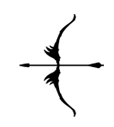
\includegraphics[width=2.08333in,height=\textheight]{images/ranger_class.png}
\end{center}

Rangers roam the borderlands, where their mission is to keep the beasts
and monsters of the untamed lands at bay. They generally operate alone
or in small groups and rely on stealth and surprise to meet their
objectives.

Humans, Elves, Half-Elves, and Halflings may become Rangers. To become a
Ranger, a character must have a Strength score of 9 or higher, Wisdom of
11 or higher, and a Dexterity of 11 or higher. They may use any weapon
and may wear any armor, but some of the Ranger's special talents and
abilities are unavailable when wearing armor heavier than leather armor.

\begin{center}
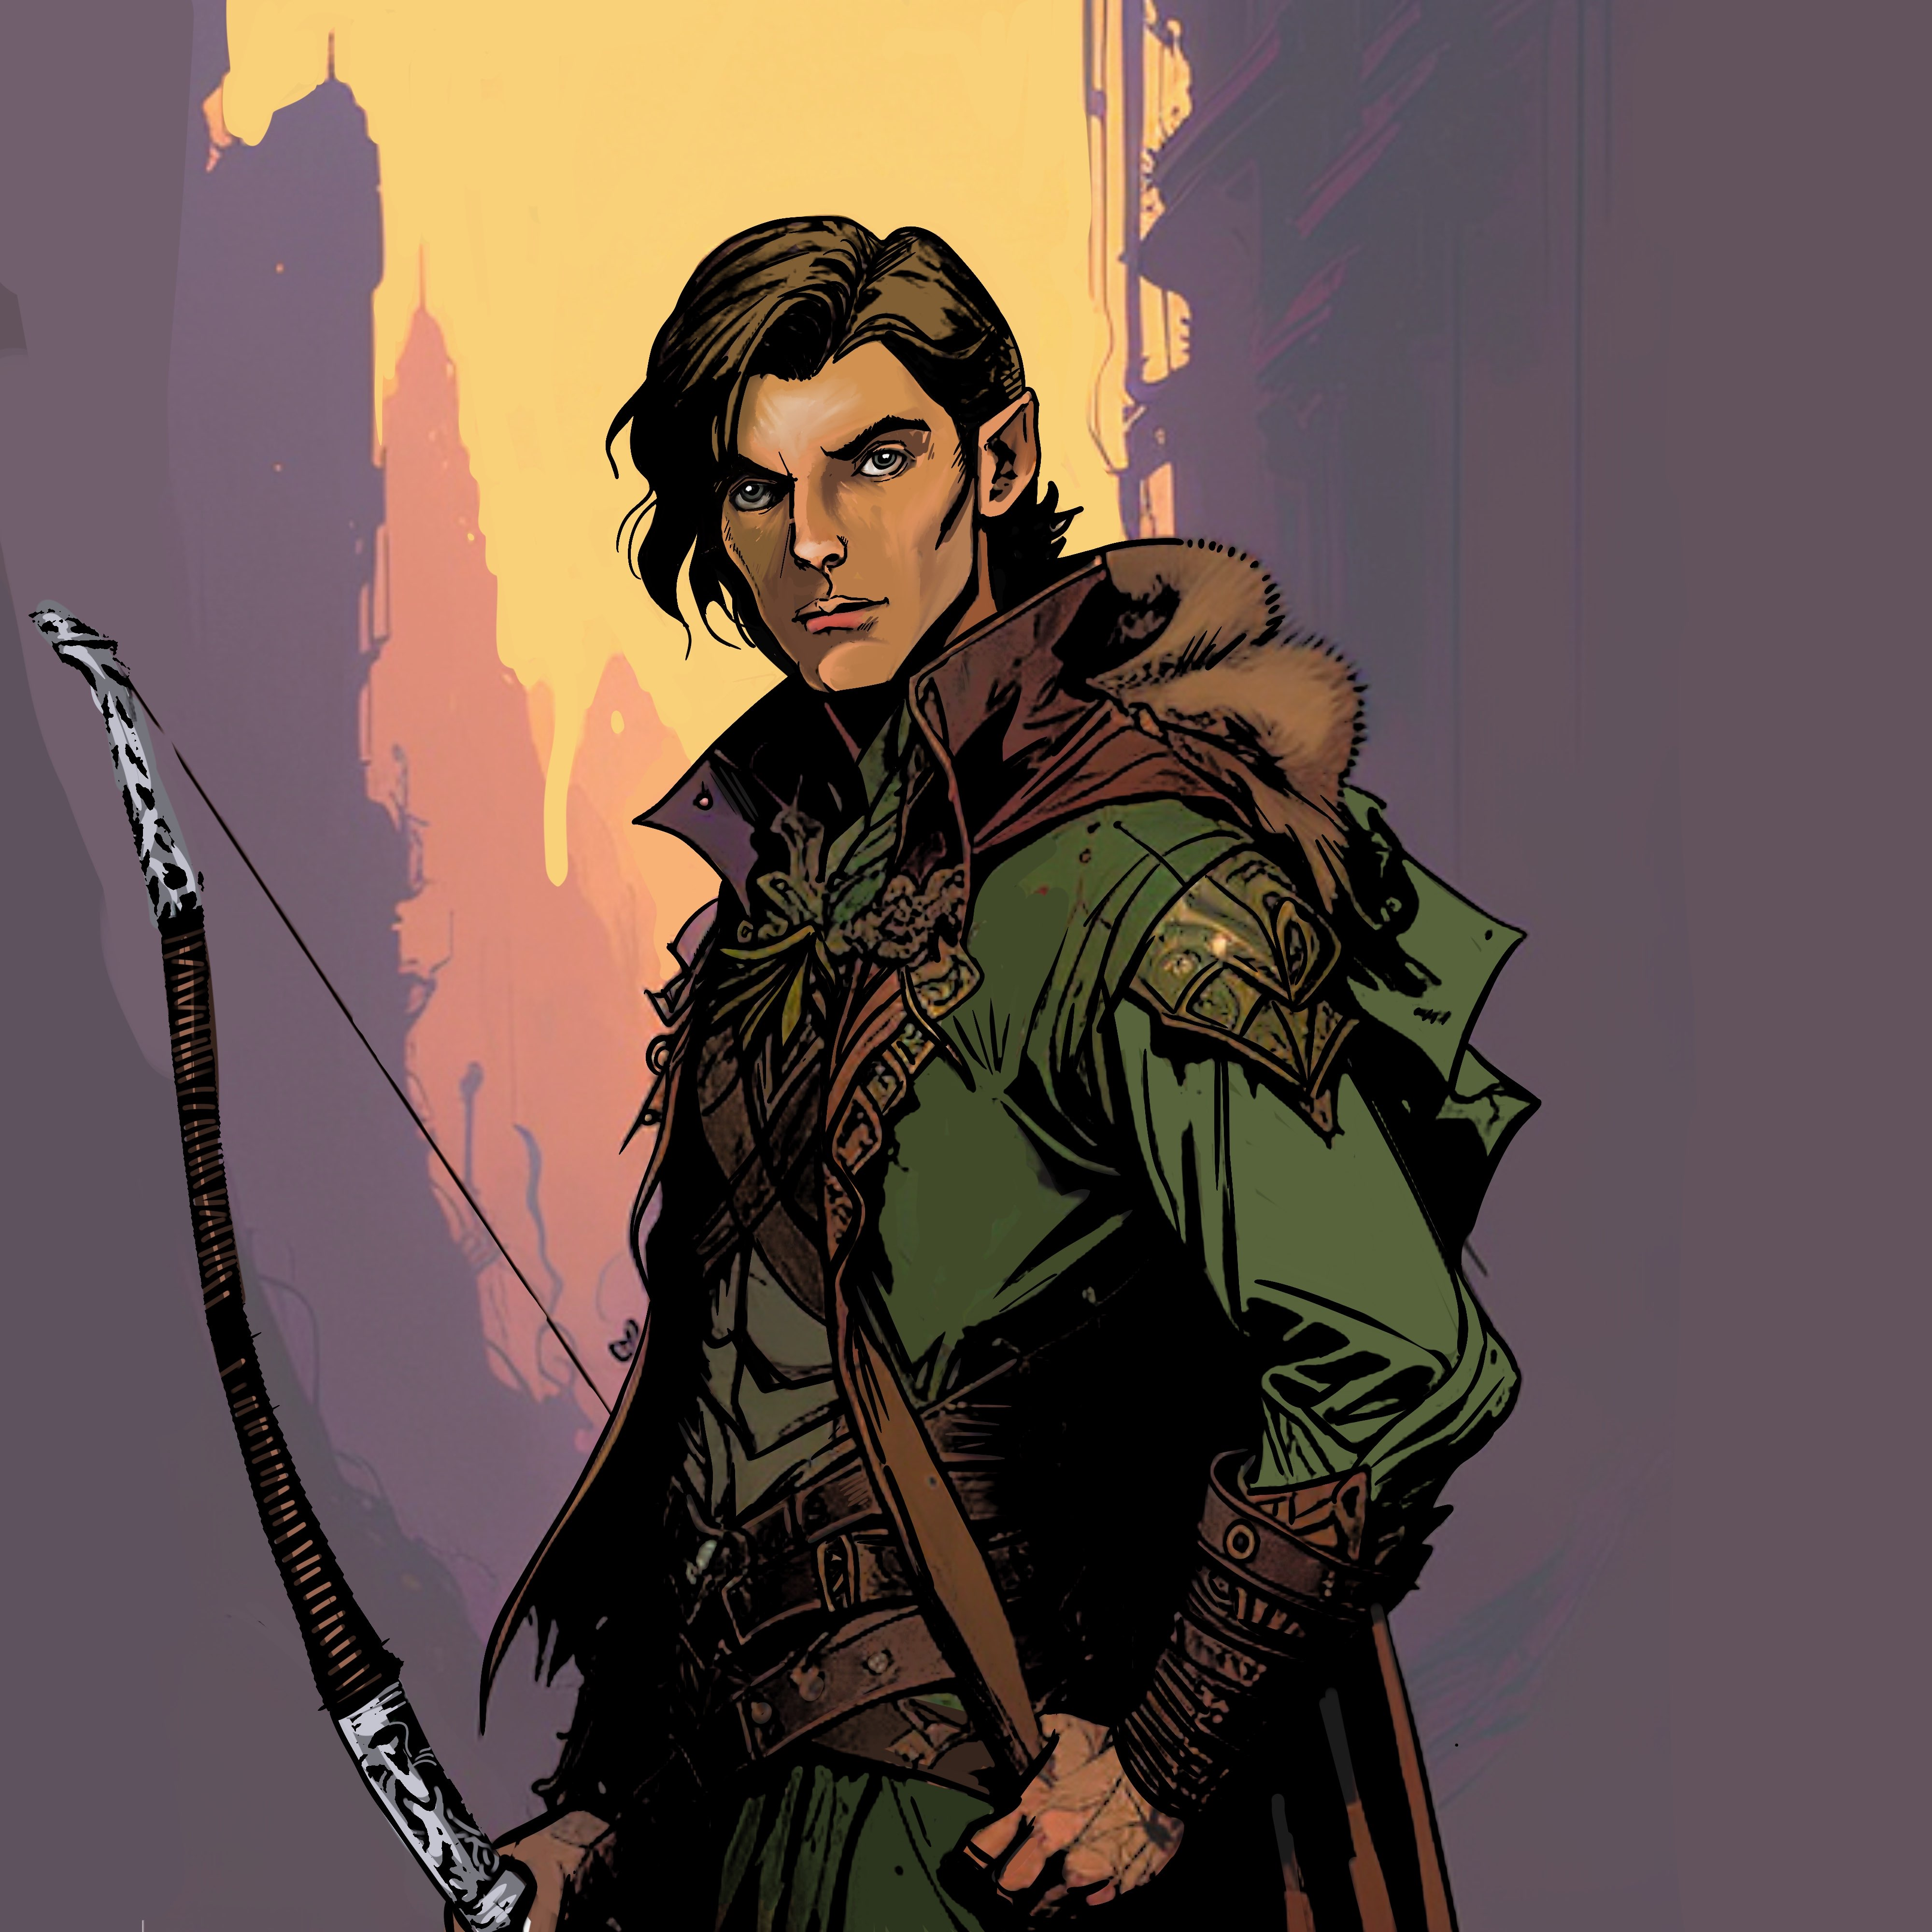
\includegraphics{images/ranger.jpg}
\end{center}

\begin{figure*}

\begin{longtable}[]{@{}
  >{\raggedright\arraybackslash}p{(\columnwidth - 14\tabcolsep) * \real{0.0625}}
  >{\raggedright\arraybackslash}p{(\columnwidth - 14\tabcolsep) * \real{0.1161}}
  >{\raggedright\arraybackslash}p{(\columnwidth - 14\tabcolsep) * \real{0.0893}}
  >{\raggedright\arraybackslash}p{(\columnwidth - 14\tabcolsep) * \real{0.1339}}
  >{\raggedright\arraybackslash}p{(\columnwidth - 14\tabcolsep) * \real{0.1786}}
  >{\raggedright\arraybackslash}p{(\columnwidth - 14\tabcolsep) * \real{0.1518}}
  >{\raggedright\arraybackslash}p{(\columnwidth - 14\tabcolsep) * \real{0.0625}}
  >{\raggedright\arraybackslash}p{(\columnwidth - 14\tabcolsep) * \real{0.2054}}@{}}
\caption{Ranger XP Progression}\label{tbl-xp-rangers}\tabularnewline
\toprule\noalign{}
\begin{minipage}[b]{\linewidth}\raggedright
Level
\end{minipage} & \begin{minipage}[b]{\linewidth}\raggedright
Exp. Points
\end{minipage} & \begin{minipage}[b]{\linewidth}\raggedright
Hit Dice
\end{minipage} & \begin{minipage}[b]{\linewidth}\raggedright
Attack Bonus
\end{minipage} & \begin{minipage}[b]{\linewidth}\raggedright
ArrowsFired/Rd
\end{minipage} & \begin{minipage}[b]{\linewidth}\raggedright
SkillPoints
\end{minipage} & \begin{minipage}[b]{\linewidth}\raggedright
Feats
\end{minipage} & \begin{minipage}[b]{\linewidth}\raggedright
WeaponProficiency
\end{minipage} \\
\midrule\noalign{}
\endfirsthead
\toprule\noalign{}
\begin{minipage}[b]{\linewidth}\raggedright
Level
\end{minipage} & \begin{minipage}[b]{\linewidth}\raggedright
Exp. Points
\end{minipage} & \begin{minipage}[b]{\linewidth}\raggedright
Hit Dice
\end{minipage} & \begin{minipage}[b]{\linewidth}\raggedright
Attack Bonus
\end{minipage} & \begin{minipage}[b]{\linewidth}\raggedright
ArrowsFired/Rd
\end{minipage} & \begin{minipage}[b]{\linewidth}\raggedright
SkillPoints
\end{minipage} & \begin{minipage}[b]{\linewidth}\raggedright
Feats
\end{minipage} & \begin{minipage}[b]{\linewidth}\raggedright
WeaponProficiency
\end{minipage} \\
\midrule\noalign{}
\endhead
\bottomrule\noalign{}
\endlastfoot
1 & 0 & 1d10 & +1 (+3 bow) & 1/1 & 3 & & 4 \\
2 & 2,200 & 2d10 & +2 (+4 bow) & 1/1 & 1 & 1 & \\
3 & 4,400 & 3 d10 & +2 (+5 bow) & 1/1 & 1 & & 1 \\
4 & 8,800 & 4d10 & +3 (+6 bow) & 1/1 & 1 & 1 & \\
5 & 17,600 & 5d10 & +4 (+7 bow) & 3/2 & 1 & & 1 \\
6 & 35,200 & 6d10 & +4 (+7 bow) & 3/2 & 1 & 1 & \\
7 & 70,400 & 7d10 & +5 (+8 bow) & 3/2 & 1 & & 1 \\
8 & 132,000 & 8d10 & +6 (+9 bow) & 3/2 & 1 & 1 & \\
9 & 264,000 & 9d10 & +6 (+9 bow) & 2/1 & 1 & & 1 \\
10 & 396,000 & 9d10+2 & +6 (+9 bow) & 2/1 & 1 & 1 & \\
11 & 528,000 & 9d10+4 & +7 (+10 bow) & 2/1 & 1 & & 1 \\
12 & 660,000 & 9d10+6 & +7 (+10 bow) & 2/1 & 1 & 1 & \\
13 & 792,000 & 9d10+8 & +8 (+11 bow) & 2/1 & 1 & & 1 \\
14 & 924,000 & 9d10+10 & +8 (+11 bow) & 2/1 & 1 & 1 & \\
15 & 1,056,000 & 9d10+12 & +8 (+11 bow) & 2/1 & 1 & & 1 \\
16 & 1,188,000 & 9d10+14 & +9 (+12 bow) & 2/1 & 1 & 1 & \\
17 & 1,320,000 & 9d10+16 & +9 (+12 bow) & 2/1 & 1 & & 1 \\
18 & 1,452,000 & 9d10+18 & +10 (+13 bow) & 2/1 & 1 & 1 & \\
19 & 1,584,000 & 9d10+20 & +10 (+13 bow) & 2/1 & 1 & & 1 \\
20 & 1,716,000 & 9d10+22 & +10(+13 bow) & 2/1 & 1 & 1 & \\
\end{longtable}

\end{figure*}%%
\begin{figure*}

\begin{longtable}[]{@{}
  >{\raggedright\arraybackslash}p{(\columnwidth - 16\tabcolsep) * \real{0.0991}}
  >{\raggedright\arraybackslash}p{(\columnwidth - 16\tabcolsep) * \real{0.0991}}
  >{\raggedright\arraybackslash}p{(\columnwidth - 16\tabcolsep) * \real{0.0811}}
  >{\raggedright\arraybackslash}p{(\columnwidth - 16\tabcolsep) * \real{0.0811}}
  >{\raggedright\arraybackslash}p{(\columnwidth - 16\tabcolsep) * \real{0.1261}}
  >{\raggedright\arraybackslash}p{(\columnwidth - 16\tabcolsep) * \real{0.1081}}
  >{\raggedright\arraybackslash}p{(\columnwidth - 16\tabcolsep) * \real{0.1171}}
  >{\raggedright\arraybackslash}p{(\columnwidth - 16\tabcolsep) * \real{0.1532}}
  >{\raggedright\arraybackslash}p{(\columnwidth - 16\tabcolsep) * \real{0.1351}}@{}}
\caption{Ranger Titles}\label{tbl-titles-rangers}\tabularnewline
\toprule\noalign{}
\begin{minipage}[b]{\linewidth}\raggedright
Alignment
\end{minipage} & \begin{minipage}[b]{\linewidth}\raggedright
Level 1
\end{minipage} & \begin{minipage}[b]{\linewidth}\raggedright
Level 2
\end{minipage} & \begin{minipage}[b]{\linewidth}\raggedright
Level 3
\end{minipage} & \begin{minipage}[b]{\linewidth}\raggedright
Level 4
\end{minipage} & \begin{minipage}[b]{\linewidth}\raggedright
Level 5
\end{minipage} & \begin{minipage}[b]{\linewidth}\raggedright
Level 9
\end{minipage} & \begin{minipage}[b]{\linewidth}\raggedright
Level 12
\end{minipage} & \begin{minipage}[b]{\linewidth}\raggedright
Level 15
\end{minipage} \\
\midrule\noalign{}
\endfirsthead
\toprule\noalign{}
\begin{minipage}[b]{\linewidth}\raggedright
Alignment
\end{minipage} & \begin{minipage}[b]{\linewidth}\raggedright
Level 1
\end{minipage} & \begin{minipage}[b]{\linewidth}\raggedright
Level 2
\end{minipage} & \begin{minipage}[b]{\linewidth}\raggedright
Level 3
\end{minipage} & \begin{minipage}[b]{\linewidth}\raggedright
Level 4
\end{minipage} & \begin{minipage}[b]{\linewidth}\raggedright
Level 5
\end{minipage} & \begin{minipage}[b]{\linewidth}\raggedright
Level 9
\end{minipage} & \begin{minipage}[b]{\linewidth}\raggedright
Level 12
\end{minipage} & \begin{minipage}[b]{\linewidth}\raggedright
Level 15
\end{minipage} \\
\midrule\noalign{}
\endhead
\bottomrule\noalign{}
\endlastfoot
Lawful & Tracker & Scout & Hunter & Pathfinder & Guardian & Ranger &
Ranger Knight & Ranger Lord \\
Neutral & Wanderer & Seeker & Forager & Trailblazer & Warden & Outrider
& Waykeeper & Forest Warden \\
Chaotic & Bandit & Stalker & Prowler & Nightblade & Manhunter &
Darkstrider & Shadow Warden & Wildreaver \\
\end{longtable}

\end{figure*}%

\begin{longtable}[]{@{}
  >{\raggedright\arraybackslash}p{(\columnwidth - 10\tabcolsep) * \real{0.1250}}
  >{\raggedright\arraybackslash}p{(\columnwidth - 10\tabcolsep) * \real{0.2273}}
  >{\raggedright\arraybackslash}p{(\columnwidth - 10\tabcolsep) * \real{0.1477}}
  >{\raggedright\arraybackslash}p{(\columnwidth - 10\tabcolsep) * \real{0.2386}}
  >{\raggedright\arraybackslash}p{(\columnwidth - 10\tabcolsep) * \real{0.1705}}
  >{\raggedright\arraybackslash}p{(\columnwidth - 10\tabcolsep) * \real{0.0909}}@{}}
\caption{Ranger Saving Throws}\label{tbl-save-ranger}\tabularnewline
\toprule\noalign{}
\begin{minipage}[b]{\linewidth}\raggedright
\textbf{Level}
\end{minipage} & \begin{minipage}[b]{\linewidth}\raggedright
Death Ray / Poison
\end{minipage} & \begin{minipage}[b]{\linewidth}\raggedright
Magic Wands
\end{minipage} & \begin{minipage}[b]{\linewidth}\raggedright
Paralysis / Petrify
\end{minipage} & \begin{minipage}[b]{\linewidth}\raggedright
Dragon Breath
\end{minipage} & \begin{minipage}[b]{\linewidth}\raggedright
Spells
\end{minipage} \\
\midrule\noalign{}
\endfirsthead
\toprule\noalign{}
\begin{minipage}[b]{\linewidth}\raggedright
\textbf{Level}
\end{minipage} & \begin{minipage}[b]{\linewidth}\raggedright
Death Ray / Poison
\end{minipage} & \begin{minipage}[b]{\linewidth}\raggedright
Magic Wands
\end{minipage} & \begin{minipage}[b]{\linewidth}\raggedright
Paralysis / Petrify
\end{minipage} & \begin{minipage}[b]{\linewidth}\raggedright
Dragon Breath
\end{minipage} & \begin{minipage}[b]{\linewidth}\raggedright
Spells
\end{minipage} \\
\midrule\noalign{}
\endhead
\bottomrule\noalign{}
\endlastfoot
1 & 12 & 13 & 14 & 15 & 17 \\
2-3 & 11 & 12 & 14 & 15 & 16 \\
4-5 & 11 & 11 & 13 & 14 & 15 \\
6-7 & 10 & 11 & 12 & 14 & 15 \\
8-9 & 9 & 10 & 12 & 13 & 14 \\
10-11 & 9 & 9 & 11 & 12 & 13 \\
12-13 & 8 & 9 & 10 & 12 & 13 \\
14-15 & 7 & 8 & 10 & 11 & 12 \\
16-17 & 7 & 7 & 9 & 10 & 11 \\
18-19 & 6 & 7 & 8 & 10 & 11 \\
20 & 5 & 6 & 8 & 9 & 10 \\
\end{longtable}

\subsection{Ranger Abilities}\label{ranger-abilities}

\subsubsection{Chosen Enemy}\label{chosen-enemy}

A Ranger must declare a chosen enemy. Against this chosen enemy, the
Ranger gets a bonus of +3 to damage. This enemy must be specific such as
giants, orcs, or dragons. It could also include rival organizations,
nations, or similar agencies.

\subsubsection{Expert Bowmen}\label{expert-bowmen}

Rangers are expert bowmen. When using any regular bow (shortbow or
longbow, but not crossbow), a Ranger adds +2 to their Attack Bonus. At
5\textsuperscript{th} level, a Ranger may fire three arrows every two
rounds (a 3/2 rate of fire). This means one attack on every odd round
and two attacks on every even round. At 9\textsuperscript{th} level, the
Ranger may fire two arrows every round, with the second attack coming at
the end of the round.

\subsubsection{Wilderness Expertise}\label{wilderness-expertise}

Rangers can Move Silently, Hide, and Track when in wilderness areas, at
percentages given in the table below. Apply a -2 penalty when attempting
these abilities in urban areas. Move Silently and Hide may not be used
in armor heavier than leather.

\begin{figure*}

\begin{longtable}[]{@{}llll@{}}
\caption{Ranger Wilderness
Expertise}\label{tbl-ranger-special-abilities}\tabularnewline
\toprule\noalign{}
Level & Move Silently (\%) & Hide (\%) & Track (\%) \\
\midrule\noalign{}
\endfirsthead
\toprule\noalign{}
Level & Move Silently (\%) & Hide (\%) & Track (\%) \\
\midrule\noalign{}
\endhead
\bottomrule\noalign{}
\endlastfoot
1 & 20 & 20 & 30 \\
2 & 25 & 25 & 35 \\
3 & 30 & 30 & 40 \\
4 & 35 & 35 & 45 \\
5 & 40 & 40 & 50 \\
6 & 45 & 45 & 55 \\
7 & 50 & 50 & 60 \\
8 & 55 & 55 & 65 \\
9 & 60 & 60 & 70 \\
10 & 65 & 65 & 75 \\
11 & 70 & 70 & 80 \\
12 & 75 & 75 & 85 \\
13 & 80 & 80 & 90 \\
14 & 85 & 85 & 95 \\
15 & 90 & 90 & 100 \\
\end{longtable}

\end{figure*}%

\section{Magic User}\label{magic-user}

\begin{center}

\includegraphics[width=2.08333in,height=\textheight]{images/magic_user_class.png}
\end{center}

Magic users are scarce. They are just as frequently reviled as they are
revered, often experiencing the shifting tides of popularity as
political dynamics ebb and flow.

\begin{itemize}
\tightlist
\item
  Everyone knows that magic exists, but it is not typical in people's
  daily lives.
\item
  It is common among the working class to think that bad things tend to
  happen whenever magic is about.
\item
  Magic items are uncommon --- hidden away in deep dungeons or put on
  display as symbols of the owner's power.
\item
  Institutions of magic are rare outside of Glantri.
\item
  Places of interest, cities, religious sites, concentrations of
  monsters, and wizard towers are all usually built on ley lines or high
  points.
\end{itemize}

Magic-Users seek and use knowledge of the arcane. They perform magic not
as the Cleric does, by faith in a greater power, but rather through
insight and understanding. Every Magic-User has a spellbook containing
the magical formulae for each spell the Magic-User has learned.
Spellbooks are written in the Arcane Language. All Magic-Users begin
play knowing how to read, write, and speak Arcane.

Magic-Users are the worst of all the classes at fighting; hours spent
studying massive tomes of magic do not lead a character to become strong
or adept with weapons. They are the least hardy, equal to Thieves at
lower levels but quickly falling behind.

The Prime Requisite for Magic-Users is Intelligence; a character must
have an Intelligence score of 9 or higher to become a Magic-User. The
only weapons they become proficient with are the dagger and the walking
staff (or cudgel). Magic-Users may not wear armor of any sort nor use a
shield as such things interfere with spellcasting.

A first-level Magic-User begins play knowing \hyperref[read-magic]{read
magic} and one other spell of first level. These spells are written in a
spellbook provided by his or her master. The DM may roll for the spell,
assign it as he or she sees fit, or allow the player to choose it, at
his or her option. See the \hyperref[magic-user-spells]{Spells} section
for more details.

\begin{center}
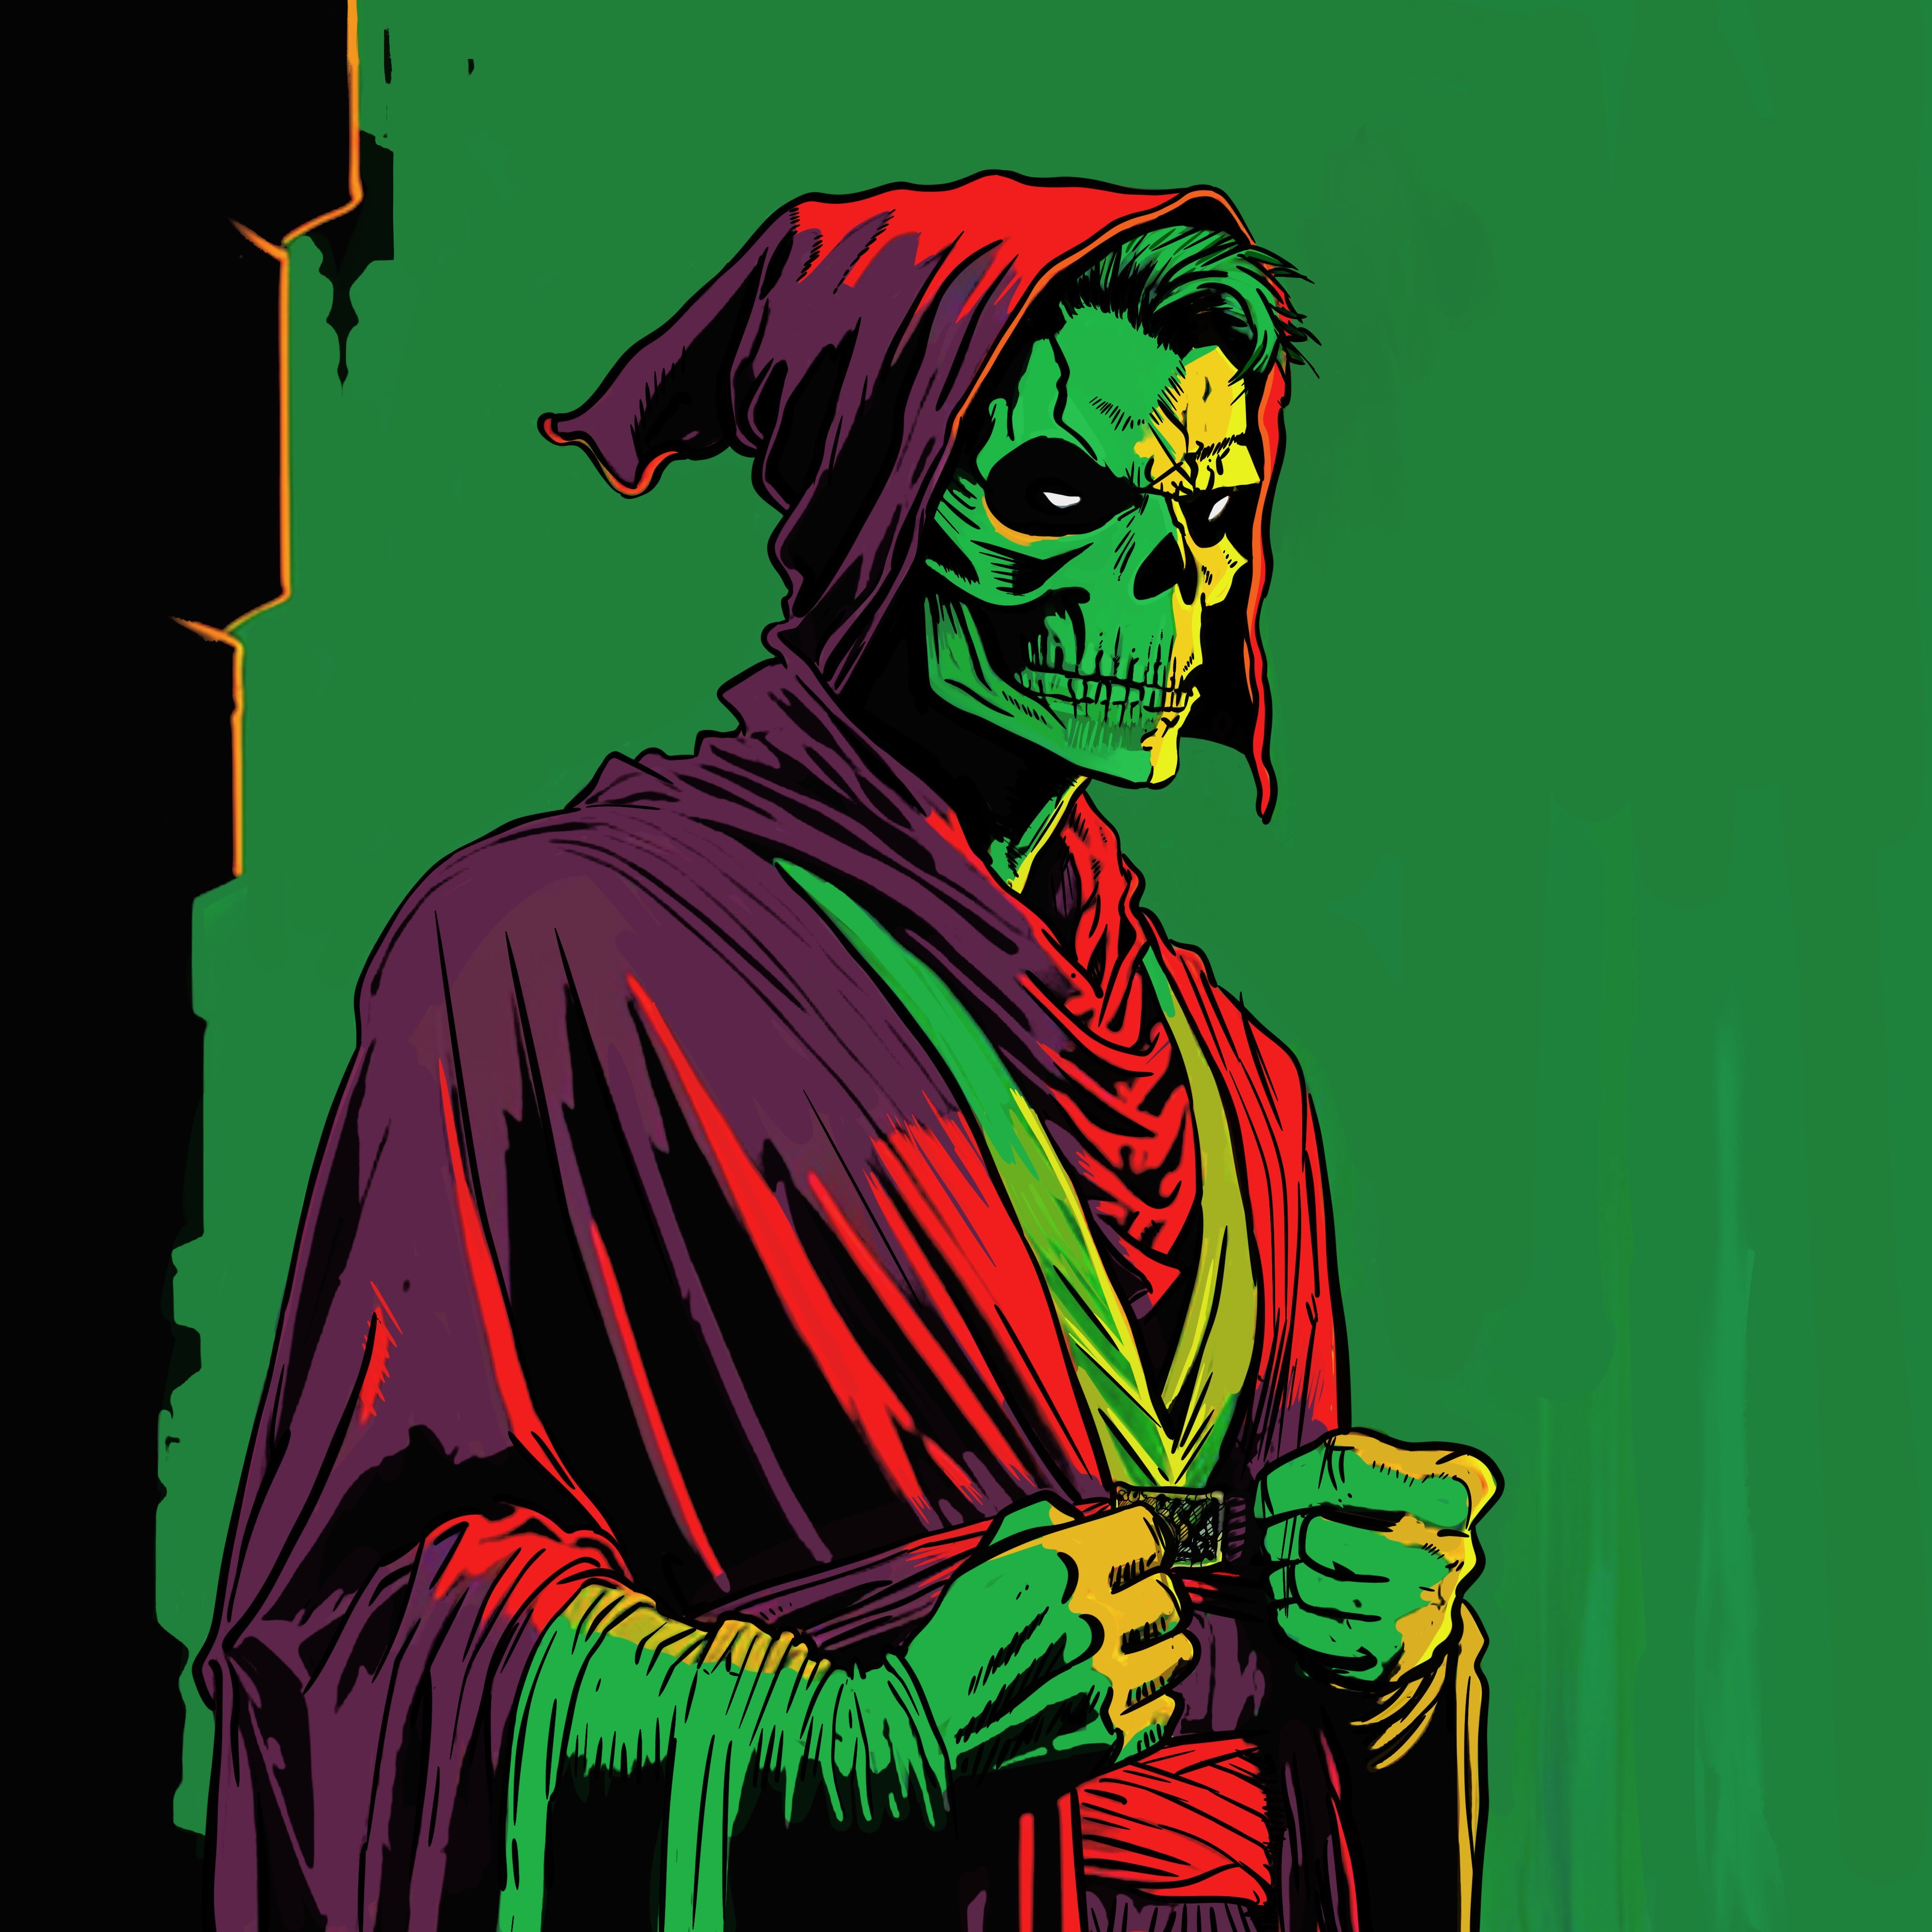
\includegraphics{images/magic_user.jpg}
\end{center}

\begin{figure*}

\begin{longtable}[]{@{}
  >{\raggedright\arraybackslash}p{(\columnwidth - 28\tabcolsep) * \real{0.0584}}
  >{\raggedleft\arraybackslash}p{(\columnwidth - 28\tabcolsep) * \real{0.1022}}
  >{\centering\arraybackslash}p{(\columnwidth - 28\tabcolsep) * \real{0.0803}}
  >{\centering\arraybackslash}p{(\columnwidth - 28\tabcolsep) * \real{0.1095}}
  >{\centering\arraybackslash}p{(\columnwidth - 28\tabcolsep) * \real{0.1095}}
  >{\raggedright\arraybackslash}p{(\columnwidth - 28\tabcolsep) * \real{0.0584}}
  >{\raggedright\arraybackslash}p{(\columnwidth - 28\tabcolsep) * \real{0.0292}}
  >{\raggedright\arraybackslash}p{(\columnwidth - 28\tabcolsep) * \real{0.0292}}
  >{\raggedright\arraybackslash}p{(\columnwidth - 28\tabcolsep) * \real{0.0292}}
  >{\raggedright\arraybackslash}p{(\columnwidth - 28\tabcolsep) * \real{0.0292}}
  >{\raggedright\arraybackslash}p{(\columnwidth - 28\tabcolsep) * \real{0.0292}}
  >{\raggedright\arraybackslash}p{(\columnwidth - 28\tabcolsep) * \real{0.0292}}
  >{\raggedright\arraybackslash}p{(\columnwidth - 28\tabcolsep) * \real{0.0292}}
  >{\raggedright\arraybackslash}p{(\columnwidth - 28\tabcolsep) * \real{0.0292}}
  >{\centering\arraybackslash}p{(\columnwidth - 28\tabcolsep) * \real{0.1533}}@{}}
\caption{Magic-User XP
Progression}\label{tbl-xp-magic-users}\tabularnewline
\toprule\noalign{}
\begin{minipage}[b]{\linewidth}\raggedright
\end{minipage} & \begin{minipage}[b]{\linewidth}\raggedleft
\end{minipage} & \begin{minipage}[b]{\linewidth}\centering
\end{minipage} & \begin{minipage}[b]{\linewidth}\centering
\end{minipage} & \begin{minipage}[b]{\linewidth}\centering
\end{minipage} & \begin{minipage}[b]{\linewidth}\raggedright
\end{minipage} & \begin{minipage}[b]{\linewidth}\raggedright
\end{minipage} & \begin{minipage}[b]{\linewidth}\raggedright
\end{minipage} &
\multicolumn{6}{>{\raggedright\arraybackslash}p{(\columnwidth - 28\tabcolsep) * \real{0.1752} + 10\tabcolsep}}{%
\begin{minipage}[b]{\linewidth}\raggedright
Spell Level
\end{minipage}} & \begin{minipage}[b]{\linewidth}\centering
\end{minipage} \\
\begin{minipage}[b]{\linewidth}\raggedright
Level
\end{minipage} & \begin{minipage}[b]{\linewidth}\raggedleft
Exp. Points
\end{minipage} & \begin{minipage}[b]{\linewidth}\centering
Hit Dice
\end{minipage} & \begin{minipage}[b]{\linewidth}\centering
Attack Bonus
\end{minipage} & \begin{minipage}[b]{\linewidth}\centering
Skill Points
\end{minipage} & \begin{minipage}[b]{\linewidth}\raggedright
Feats
\end{minipage} & \begin{minipage}[b]{\linewidth}\raggedright
0
\end{minipage} & \begin{minipage}[b]{\linewidth}\raggedright
1
\end{minipage} & \begin{minipage}[b]{\linewidth}\raggedright
2
\end{minipage} & \begin{minipage}[b]{\linewidth}\raggedright
3
\end{minipage} & \begin{minipage}[b]{\linewidth}\raggedright
4
\end{minipage} & \begin{minipage}[b]{\linewidth}\raggedright
5
\end{minipage} & \begin{minipage}[b]{\linewidth}\raggedright
6
\end{minipage} & \begin{minipage}[b]{\linewidth}\raggedright
7
\end{minipage} & \begin{minipage}[b]{\linewidth}\centering
Weapon Proficiency
\end{minipage} \\
\midrule\noalign{}
\endfirsthead
\toprule\noalign{}
\begin{minipage}[b]{\linewidth}\raggedright
\end{minipage} & \begin{minipage}[b]{\linewidth}\raggedleft
\end{minipage} & \begin{minipage}[b]{\linewidth}\centering
\end{minipage} & \begin{minipage}[b]{\linewidth}\centering
\end{minipage} & \begin{minipage}[b]{\linewidth}\centering
\end{minipage} & \begin{minipage}[b]{\linewidth}\raggedright
\end{minipage} & \begin{minipage}[b]{\linewidth}\raggedright
\end{minipage} & \begin{minipage}[b]{\linewidth}\raggedright
\end{minipage} &
\multicolumn{6}{>{\raggedright\arraybackslash}p{(\columnwidth - 28\tabcolsep) * \real{0.1752} + 10\tabcolsep}}{%
\begin{minipage}[b]{\linewidth}\raggedright
Spell Level
\end{minipage}} & \begin{minipage}[b]{\linewidth}\centering
\end{minipage} \\
\begin{minipage}[b]{\linewidth}\raggedright
Level
\end{minipage} & \begin{minipage}[b]{\linewidth}\raggedleft
Exp. Points
\end{minipage} & \begin{minipage}[b]{\linewidth}\centering
Hit Dice
\end{minipage} & \begin{minipage}[b]{\linewidth}\centering
Attack Bonus
\end{minipage} & \begin{minipage}[b]{\linewidth}\centering
Skill Points
\end{minipage} & \begin{minipage}[b]{\linewidth}\raggedright
Feats
\end{minipage} & \begin{minipage}[b]{\linewidth}\raggedright
0
\end{minipage} & \begin{minipage}[b]{\linewidth}\raggedright
1
\end{minipage} & \begin{minipage}[b]{\linewidth}\raggedright
2
\end{minipage} & \begin{minipage}[b]{\linewidth}\raggedright
3
\end{minipage} & \begin{minipage}[b]{\linewidth}\raggedright
4
\end{minipage} & \begin{minipage}[b]{\linewidth}\raggedright
5
\end{minipage} & \begin{minipage}[b]{\linewidth}\raggedright
6
\end{minipage} & \begin{minipage}[b]{\linewidth}\raggedright
7
\end{minipage} & \begin{minipage}[b]{\linewidth}\centering
Weapon Proficiency
\end{minipage} \\
\midrule\noalign{}
\endhead
\bottomrule\noalign{}
\endlastfoot
1 & 0 & 1d4 & +1 & 3 & & 1 & 1 & -- & -- & -- & -- & -- & -- & 2 \\
2 & 2,500 & 2d4 & +1 & 1 & 1 & 2 & 2 & -- & -- & -- & -- & -- & -- & \\
3 & 5,000 & 3d4 & +1 & 1 & & 3 & 2 & 1 & -- & -- & -- & -- & -- & \\
4 & 10,000 & 4d4 & +2 & 1 & 1 & 4 & 2 & 2 & -- & -- & -- & -- & -- & \\
5 & 20,000 & 5d4 & +2 & 1 & & 5 & 2 & 2 & 1 & -- & -- & -- & -- & \\
6 & 40,000 & 6d4 & +3 & 1 & 1 & 6 & 3 & 2 & 2 & -- & -- & -- & -- & \\
7 & 80,000 & 7d4 & +3 & 1 & & 7 & 3 & 2 & 2 & 1 & -- & -- & -- & \\
8 & 150,000 & 8d4 & +3 & 1 & 1 & 8 & 3 & 3 & 2 & 2 & -- & -- & -- & \\
9 & 300,000 & 9d4 & +4 & 1 & & 9 & 3 & 3 & 2 & 2 & 1 & -- & -- & \\
10 & 450,000 & 9d4+1 & +4 & 1 & 1 & 9 & 4 & 3 & 3 & 2 & 2 & -- & -- & \\
11 & 600,000 & 9d4+2 & +4 & 1 & & 9 & 4 & 4 & 3 & 2 & 2 & 1 & -- & \\
12 & 750,000 & 9d4+3 & +4 & 1 & 1 & 9 & 4 & 4 & 3 & 3 & 2 & 2 & -- & \\
13 & 900,000 & 9d4+4 & +5 & 1 & & 9 & 4 & 4 & 4 & 3 & 2 & 2 & 1 & \\
14 & 1,050,000 & 9d4+5 & +5 & 1 & 1 & 9 & 4 & 4 & 4 & 3 & 3 & 2 & 1 & \\
15 & 1,200,000 & 9d4+6 & +5 & 1 & & 9 & 5 & 4 & 4 & 3 & 3 & 2 & 1 & \\
16 & 1,350,000 & 9d4+7 & +6 & 1 & 1 & 9 & 5 & 5 & 4 & 3 & 3 & 2 & 2 & \\
17 & 1,500,000 & 9d4+8 & +6 & 1 & & 9 & 5 & 5 & 4 & 4 & 3 & 3 & 2 & \\
18 & 1,650,000 & 9d4+9 & +6 & 1 & 1 & 9 & 6 & 5 & 4 & 4 & 3 & 3 & 2 & \\
19 & 1,800,000 & 9d4+10 & +7 & 1 & & 9 & 6 & 5 & 5 & 4 & 3 & 3 & 2 & \\
20 & 1,950,000 & 9d4+11 & +7 & 1 & 1 & 9 & 6 & 5 & 5 & 4 & 4 & 3 & 3
& \\
\end{longtable}

\end{figure*}%%
\begin{figure*}

\begin{longtable}[]{@{}
  >{\raggedright\arraybackslash}p{(\columnwidth - 16\tabcolsep) * \real{0.0982}}
  >{\raggedright\arraybackslash}p{(\columnwidth - 16\tabcolsep) * \real{0.1161}}
  >{\raggedright\arraybackslash}p{(\columnwidth - 16\tabcolsep) * \real{0.1071}}
  >{\raggedright\arraybackslash}p{(\columnwidth - 16\tabcolsep) * \real{0.1071}}
  >{\raggedright\arraybackslash}p{(\columnwidth - 16\tabcolsep) * \real{0.1250}}
  >{\raggedright\arraybackslash}p{(\columnwidth - 16\tabcolsep) * \real{0.1161}}
  >{\raggedright\arraybackslash}p{(\columnwidth - 16\tabcolsep) * \real{0.0982}}
  >{\raggedright\arraybackslash}p{(\columnwidth - 16\tabcolsep) * \real{0.1250}}
  >{\raggedright\arraybackslash}p{(\columnwidth - 16\tabcolsep) * \real{0.1071}}@{}}
\caption{Magic-User Titles}\label{tbl-titles-magic-users}\tabularnewline
\toprule\noalign{}
\begin{minipage}[b]{\linewidth}\raggedright
Alignment
\end{minipage} & \begin{minipage}[b]{\linewidth}\raggedright
Level 1
\end{minipage} & \begin{minipage}[b]{\linewidth}\raggedright
Level 2
\end{minipage} & \begin{minipage}[b]{\linewidth}\raggedright
Level 3
\end{minipage} & \begin{minipage}[b]{\linewidth}\raggedright
Level 4
\end{minipage} & \begin{minipage}[b]{\linewidth}\raggedright
Level 5
\end{minipage} & \begin{minipage}[b]{\linewidth}\raggedright
Level 9
\end{minipage} & \begin{minipage}[b]{\linewidth}\raggedright
Level 12
\end{minipage} & \begin{minipage}[b]{\linewidth}\raggedright
Level 15
\end{minipage} \\
\midrule\noalign{}
\endfirsthead
\toprule\noalign{}
\begin{minipage}[b]{\linewidth}\raggedright
Alignment
\end{minipage} & \begin{minipage}[b]{\linewidth}\raggedright
Level 1
\end{minipage} & \begin{minipage}[b]{\linewidth}\raggedright
Level 2
\end{minipage} & \begin{minipage}[b]{\linewidth}\raggedright
Level 3
\end{minipage} & \begin{minipage}[b]{\linewidth}\raggedright
Level 4
\end{minipage} & \begin{minipage}[b]{\linewidth}\raggedright
Level 5
\end{minipage} & \begin{minipage}[b]{\linewidth}\raggedright
Level 9
\end{minipage} & \begin{minipage}[b]{\linewidth}\raggedright
Level 12
\end{minipage} & \begin{minipage}[b]{\linewidth}\raggedright
Level 15
\end{minipage} \\
\midrule\noalign{}
\endhead
\bottomrule\noalign{}
\endlastfoot
Lawful & Apprentice & Conjurer & Magician & Spellbinder & Arcanist &
Wizard & Mage & Arch Mage \\
Neutral & Novice & Hedge Mage & Seer & Sage & Diviner & Magus &
Mystagogue & Arch Magus \\
Chaotic & Warlock & Channeler & Hexcrafter & Spellbreaker & Chaosmancer
& Sorcerer & Diabolist & Sorcerous Master \\
\end{longtable}

\end{figure*}%

\begin{longtable}[]{@{}ll@{}}
\caption{Magic-User Intelligence
Bonus}\label{tbl-intelligence-magic-users}\tabularnewline
\toprule\noalign{}
Intelligence & Spell Bonus \\
\midrule\noalign{}
\endfirsthead
\toprule\noalign{}
Intelligence & Spell Bonus \\
\midrule\noalign{}
\endhead
\bottomrule\noalign{}
\endlastfoot
9-11 & No bonus spells \\
12 & +1 Cantrip \\
13-15 & +1 Cantrip, +1 1\textsuperscript{st} level spell \\
16-17 & +2 Cantrips, +2 1\textsuperscript{st} level spells \\
18 & +3 Cantrips, +3 1\textsuperscript{st} level, +1
2\textsuperscript{nd} level spells \\
\end{longtable}

\begin{longtable}[]{@{}
  >{\raggedright\arraybackslash}p{(\columnwidth - 10\tabcolsep) * \real{0.1250}}
  >{\raggedright\arraybackslash}p{(\columnwidth - 10\tabcolsep) * \real{0.2273}}
  >{\raggedright\arraybackslash}p{(\columnwidth - 10\tabcolsep) * \real{0.1477}}
  >{\raggedright\arraybackslash}p{(\columnwidth - 10\tabcolsep) * \real{0.2386}}
  >{\raggedright\arraybackslash}p{(\columnwidth - 10\tabcolsep) * \real{0.1705}}
  >{\raggedright\arraybackslash}p{(\columnwidth - 10\tabcolsep) * \real{0.0909}}@{}}
\caption{Magic-User Saving Throws}\label{tbl-save-mage}\tabularnewline
\toprule\noalign{}
\begin{minipage}[b]{\linewidth}\raggedright
\textbf{Level}
\end{minipage} & \begin{minipage}[b]{\linewidth}\raggedright
Death Ray / Poison
\end{minipage} & \begin{minipage}[b]{\linewidth}\raggedright
Magic Wands
\end{minipage} & \begin{minipage}[b]{\linewidth}\raggedright
Paralysis / Petrify
\end{minipage} & \begin{minipage}[b]{\linewidth}\raggedright
Dragon Breath
\end{minipage} & \begin{minipage}[b]{\linewidth}\raggedright
Spells
\end{minipage} \\
\midrule\noalign{}
\endfirsthead
\toprule\noalign{}
\begin{minipage}[b]{\linewidth}\raggedright
\textbf{Level}
\end{minipage} & \begin{minipage}[b]{\linewidth}\raggedright
Death Ray / Poison
\end{minipage} & \begin{minipage}[b]{\linewidth}\raggedright
Magic Wands
\end{minipage} & \begin{minipage}[b]{\linewidth}\raggedright
Paralysis / Petrify
\end{minipage} & \begin{minipage}[b]{\linewidth}\raggedright
Dragon Breath
\end{minipage} & \begin{minipage}[b]{\linewidth}\raggedright
Spells
\end{minipage} \\
\midrule\noalign{}
\endhead
\bottomrule\noalign{}
\endlastfoot
\textbf{1} & 13 & 14 & 13 & 16 & 15 \\
\textbf{2-3} & 13 & 14 & 13 & 15 & 14 \\
\textbf{4-5} & 12 & 13 & 12 & 15 & 13 \\
\textbf{6-7} & 12 & 12 & 11 & 14 & 13 \\
\textbf{8-9} & 11 & 11 & 10 & 14 & 12 \\
\textbf{10-11} & 11 & 10 & 9 & 13 & 11 \\
\textbf{12-13} & 10 & 10 & 9 & 13 & 11 \\
\textbf{14-15} & 10 & 9 & 8 & 12 & 10 \\
\textbf{16-17} & 9 & 8 & 7 & 12 & 9 \\
\textbf{18-19} & 9 & 7 & 6 & 11 & 9 \\
\textbf{20} & 8 & 6 & 5 & 11 & 8 \\
\end{longtable}

\subsection{Magic-User Abilities}\label{magic-user-abilities}

\subsubsection{Starting Spells}\label{starting-spells}

A first level Magic-User begins play with inherent Detect Magic,
\hyperref[read-magic]{Read Magic} and \hyperref[arcane-bolt]{Arcane
Bolt}. The player can also choose one 0 Level Spell and one 1 level
Spell. The DM rolls any additional 0 and 1 spells randomly.

\subsubsection{Inherent Detect Magic}\label{inherent-detect-magic}

Magic-Users can detect magic in anything they touch. Magical items or
creatures feel warm, cause a tingling sensation, or have some other
unusual tactile effect.

\subsubsection{Inherent Read Magic}\label{inherent-read-magic}

Magic-Users can read and write magic (Arcane) without a spell. The
arcane language was discovered by Magic-Users (not invented). Arcane
language is the same no matter what the native language or culture of
the spell caster.

\subsubsection{Arcane Bolt}\label{arcane-bolt}

This is a bolt of raw magic. The target gets a save vs.~spells to avoid
all damage. The bolt has a range of 30 feet and does 1d4 damage. Since
it is pure magic, it will affect creatures only affected by magical
weapons. The Arcane Bolt does not affect inanimate objects.

\subsubsection{Spell Preparation}\label{spell-preparation}

A Magic-User may only prepare spells after resting and needs one turn
per each three spell levels to do so. Spells prepared but not used on a
previous day are not lost. For example, a 3rd level Magic-User preparing
all three of their available spells (two 1st level and one 2nd level) is
preparing a total of 4 levels of spells, and thus needs 2 turns (4
divided by 3 and rounded up). Each day, usually in the morning,
spellcasters prepare spells by studying their spellbooks to replace
those they have used. Spells prepared but not used persist from day to
day; only those cast must be replaced. A spellcaster may always choose
to dismiss a prepared spell (without casting it) to prepare a different
spell of that level.

\subsubsection{Casting}\label{casting}

Magic-Users must have at least one hand free and be able to speak to
cast spells. Binding and gagging a spellcaster is an effective means of
preventing spell casting. In combat, casting a spell takes the same time
as making an attack

\subsubsection{Spell Disruption}\label{spell-disruption}

If a Magic-User is attacked (even if not hit), the character must make a
saving throw vs.~spells on the Initiative number on which they are
casting a spell. On a failure, the spell is spoiled and lost. As a
specific exception, two spell casters releasing their spells at each
other on the same Initiative number will both succeed in their casting;
one caster may disrupt another with a spell only if they have a better
initiative and chooses to delay casting the spell until right before the
other caster.

\subsubsection{Learning New Spells}\label{learning-new-spells}

A Magic-User may learn spells by being taught directly by another magic
user, by studying, by transcribing from a spell scroll or another
individual's spellbook, or through research. If being taught, a spell
can be learned in a single day, while referencing another individual's
spellbook takes one day per spell level. It typically costs 300 gps per
spell level.

To copy a spell, the character must spend 1d4 hours per Spell Level. The
chance of successfully mastering a spell is DC 12 -1 per level of the
magic-user, - INT bonus, +1 per level of the spell. Any failure requires
another Magic-User who knows the spell to teach it. Spell mastery
failure isn't black and white. Spells that aren't mastered may be cast
but require a D20 check on the Potential Spell Failure Table.

\begin{longtable}[]{@{}
  >{\raggedright\arraybackslash}p{(\columnwidth - 2\tabcolsep) * \real{0.0609}}
  >{\raggedright\arraybackslash}p{(\columnwidth - 2\tabcolsep) * \real{0.9391}}@{}}
\caption{Potential Spell Failure
Table}\label{tbl-potential-spell-failure}\tabularnewline
\toprule\noalign{}
\begin{minipage}[b]{\linewidth}\raggedright
Roll
\end{minipage} & \begin{minipage}[b]{\linewidth}\raggedright
Effect
\end{minipage} \\
\midrule\noalign{}
\endfirsthead
\toprule\noalign{}
\begin{minipage}[b]{\linewidth}\raggedright
Roll
\end{minipage} & \begin{minipage}[b]{\linewidth}\raggedright
Effect
\end{minipage} \\
\midrule\noalign{}
\endhead
\bottomrule\noalign{}
\endlastfoot
1 & Spell fails entirely. A demon or other hostile entity appropriate to
the setting appears and attacks the caster. \\
2-4 & Spell fails entirely. Caster takes 1d6 points of injury. \\
5-7 & Spell fails entirely. Caster temporarily forgets the spell. Make a
DC10 Int roll after a week, and again each following week, until they
remember. \\
8-10 & Spell has the reverse of the intended effect. \\
11-12 & Spell affects someone or something other than its intended
target -- friend, foe, or random object. \\
13-14 & Spell produces nothing but a loud noise, bright flash of light,
awful odor, etc. \\
15-17 & Spell produces a weaker version of the intended effect. \\
18-20 & Spell is cast normally. \\
\end{longtable}

\subsubsection{Great School of Magic in
Glantri}\label{great-school-of-magic-in-glantri}

The Great School of Magic in Glantri City is a place of arcane learning
and the heart of Glantrian society. While many magic-users have been
privately tutored, the best and brightest come from the Great School.
There are 4 two-month quarters at the school separated by month long
breaks. One on one mentoring continues until the Magic-User is 4th level
at which point they are released to independent study. Routine testing
is still administered until 6th level at which time the Magic-User
graduates and is formally declared a Magic-User. After that time, they
may stay at the school to use the facilities and take Arcana courses,
but this is usually frowned upon.

\paragraph{Great School of Magic Costs and
Expenses}\label{great-school-of-magic-costs-and-expenses}

The tuition for the Great School is 300 gp per spell level. One week is
required per spell level to complete the research. Tuition covers access
to the facilities, mentor, classes, and common needs such as ink and
paper. Thrown in for free are a small room and three (poor) meals a day
for those who want it.

\paragraph{Arcane Symbols}\label{arcane-symbols}

Magic-Users trained at Great School of Magic will be familar with the
runes identifying potions created by the School's Master Alchemist.
Kappiyan Flurmastyr is the current Master Alchemist.

\begin{center}
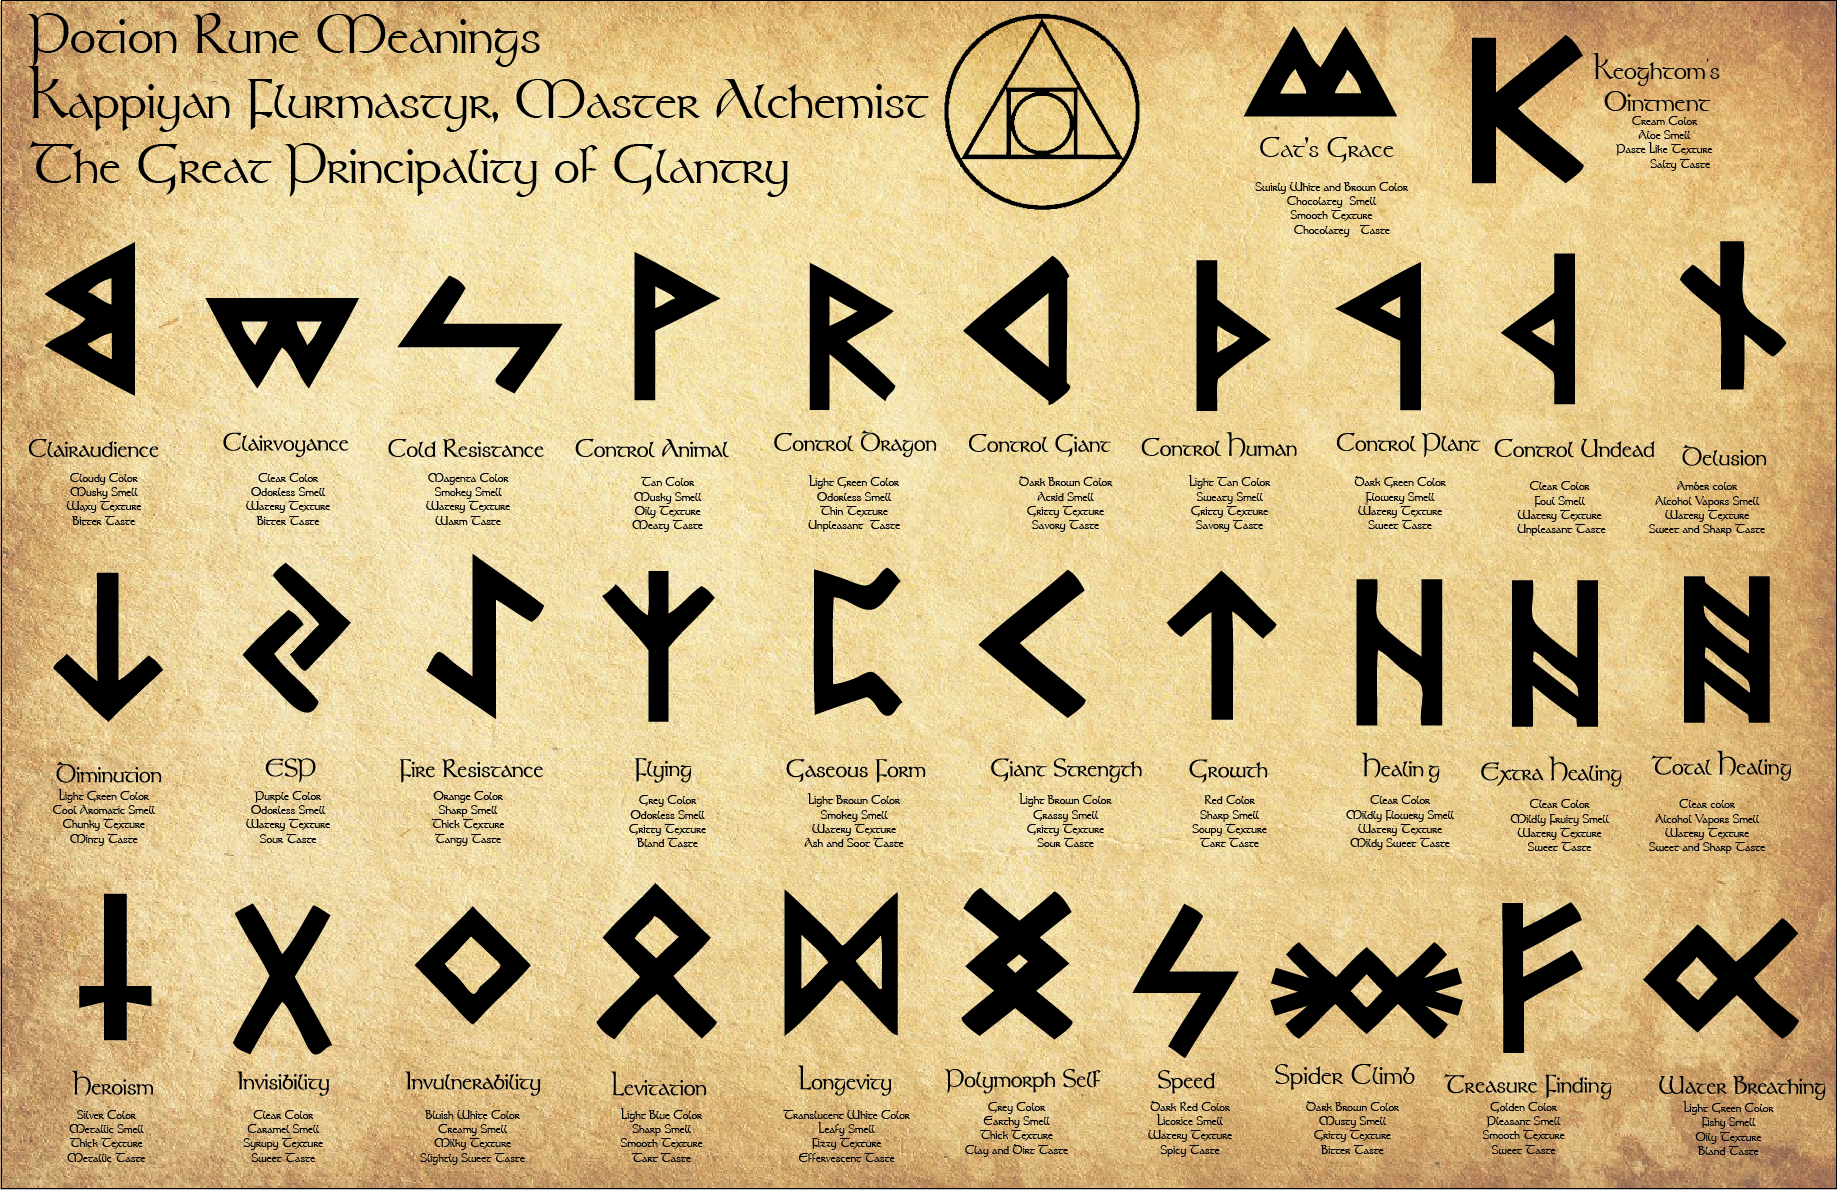
\includegraphics{images/potions.png}
\end{center}

Magic-Users will also recognize certain arcane symbols representing the
four basic elements.

\begin{center}
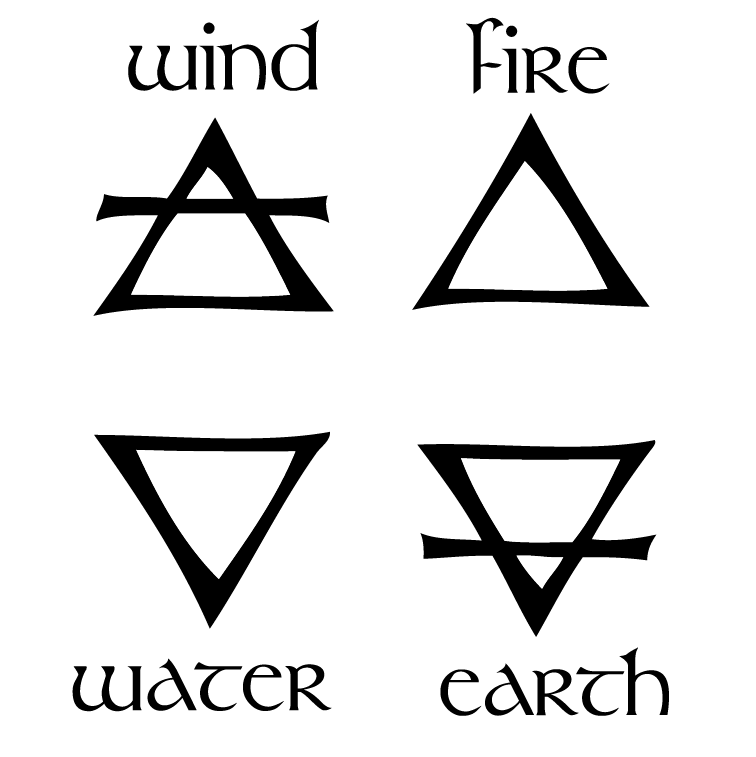
\includegraphics{images/elementalSymbols.png}
\end{center}

\section{Thief}\label{thief}

\begin{center}

\includegraphics{images/thief_class.png}
\end{center}

Thieves are those who take what they want or need by stealth, disarming
traps and picking locks to get to the gold they crave; or ``borrowing''
money from pockets, beltpouches, etc. right under the nose of the
``mark'' without the victim ever knowing.

Thieves fight better than Magic-Users but not as well as Fighters.
Avoidance of honest work leads Thieves to be less hardy than the other
classes, though they do pull ahead of the Magic-Users at higher levels.

\begin{center}

\includegraphics[width=41.66667in,height=\textheight]{images/thief.jpg}
\end{center}

The Prime Requisite for Thieves is Dexterity; a character must have a
Dexterity score of 9 or higher to become a Thief. They may use any
weapon, but may not wear metal armor as it interferes with stealthy
activities, nor may they use shields of any sort. Leather armor is
acceptable, however.

\begin{figure*}

\begin{longtable}[]{@{}
  >{\raggedright\arraybackslash}p{(\columnwidth - 12\tabcolsep) * \real{0.0745}}
  >{\raggedright\arraybackslash}p{(\columnwidth - 12\tabcolsep) * \real{0.1383}}
  >{\raggedright\arraybackslash}p{(\columnwidth - 12\tabcolsep) * \real{0.1064}}
  >{\raggedright\arraybackslash}p{(\columnwidth - 12\tabcolsep) * \real{0.1809}}
  >{\raggedright\arraybackslash}p{(\columnwidth - 12\tabcolsep) * \real{0.1809}}
  >{\raggedright\arraybackslash}p{(\columnwidth - 12\tabcolsep) * \real{0.0745}}
  >{\raggedright\arraybackslash}p{(\columnwidth - 12\tabcolsep) * \real{0.2447}}@{}}
\caption{Thief XP Progression}\label{tbl-xp-thieves}\tabularnewline
\toprule\noalign{}
\begin{minipage}[b]{\linewidth}\raggedright
Level
\end{minipage} & \begin{minipage}[b]{\linewidth}\raggedright
Exp. Points
\end{minipage} & \begin{minipage}[b]{\linewidth}\raggedright
Hit Dice
\end{minipage} & \begin{minipage}[b]{\linewidth}\raggedright
AttackBonus
\end{minipage} & \begin{minipage}[b]{\linewidth}\raggedright
SkillPoints
\end{minipage} & \begin{minipage}[b]{\linewidth}\raggedright
Feats
\end{minipage} & \begin{minipage}[b]{\linewidth}\raggedright
WeaponProficiency
\end{minipage} \\
\midrule\noalign{}
\endfirsthead
\toprule\noalign{}
\begin{minipage}[b]{\linewidth}\raggedright
Level
\end{minipage} & \begin{minipage}[b]{\linewidth}\raggedright
Exp. Points
\end{minipage} & \begin{minipage}[b]{\linewidth}\raggedright
Hit Dice
\end{minipage} & \begin{minipage}[b]{\linewidth}\raggedright
AttackBonus
\end{minipage} & \begin{minipage}[b]{\linewidth}\raggedright
SkillPoints
\end{minipage} & \begin{minipage}[b]{\linewidth}\raggedright
Feats
\end{minipage} & \begin{minipage}[b]{\linewidth}\raggedright
WeaponProficiency
\end{minipage} \\
\midrule\noalign{}
\endhead
\bottomrule\noalign{}
\endlastfoot
1 & 0 & 1d6 & +1 & 3 & & 3 \\
2 & 1,250 & 2d6 & +1 & 1 & 1 & \\
3 & 2,500 & 3d6 & +2 & 1 & & \\
4 & 5,000 & 4d6 & +2 & 1 & 1 & 1 \\
5 & 10,000 & 5d6 & +3 & 1 & & \\
6 & 20,000 & 6d6 & +3 & 1 & 1 & \\
7 & 40,000 & 7d6 & +4 & 1 & & 1 \\
8 & 75,000 & 8d6 & +4 & 1 & 1 & \\
9 & 150,000 & 9d6 & +5 & 1 & & \\
10 & 225,000 & 9d6+2 & +5 & 1 & 1 & 1 \\
11 & 300,000 & 9d6+4 & +5 & 1 & & \\
12 & 375,000 & 9d6+6 & +6 & 1 & 1 & \\
13 & 450,000 & 9d6+8 & +6 & 1 & & 1 \\
14 & 525,000 & 9d6+10 & +6 & 1 & 1 & \\
15 & 600,000 & 9d6+12 & +7 & 1 & & \\
16 & 675,000 & 9d6+14 & +7 & 1 & 1 & 1 \\
17 & 750,000 & 9d6+16 & +7 & 1 & & \\
18 & 825,000 & 9d6+18 & +8 & 1 & 1 & \\
19 & 900,000 & 9d6+20 & +8 & 1 & & 1 \\
20 & 975,000 & 9d6+22 & +8 & 1 & 1 & \\
\end{longtable}

\end{figure*}%%
\begin{figure*}

\begin{longtable}[]{@{}
  >{\raggedright\arraybackslash}p{(\columnwidth - 16\tabcolsep) * \real{0.1000}}
  >{\raggedright\arraybackslash}p{(\columnwidth - 16\tabcolsep) * \real{0.0909}}
  >{\raggedright\arraybackslash}p{(\columnwidth - 16\tabcolsep) * \real{0.1091}}
  >{\raggedright\arraybackslash}p{(\columnwidth - 16\tabcolsep) * \real{0.1273}}
  >{\raggedright\arraybackslash}p{(\columnwidth - 16\tabcolsep) * \real{0.1273}}
  >{\raggedright\arraybackslash}p{(\columnwidth - 16\tabcolsep) * \real{0.1182}}
  >{\raggedright\arraybackslash}p{(\columnwidth - 16\tabcolsep) * \real{0.1000}}
  >{\raggedright\arraybackslash}p{(\columnwidth - 16\tabcolsep) * \real{0.1182}}
  >{\raggedright\arraybackslash}p{(\columnwidth - 16\tabcolsep) * \real{0.1091}}@{}}
\caption{Thieve's Titles}\label{tbl-titles-thieves}\tabularnewline
\toprule\noalign{}
\begin{minipage}[b]{\linewidth}\raggedright
Alignment
\end{minipage} & \begin{minipage}[b]{\linewidth}\raggedright
Level 1
\end{minipage} & \begin{minipage}[b]{\linewidth}\raggedright
Level 2
\end{minipage} & \begin{minipage}[b]{\linewidth}\raggedright
Level 3
\end{minipage} & \begin{minipage}[b]{\linewidth}\raggedright
Level 4
\end{minipage} & \begin{minipage}[b]{\linewidth}\raggedright
Level 5
\end{minipage} & \begin{minipage}[b]{\linewidth}\raggedright
Level 9
\end{minipage} & \begin{minipage}[b]{\linewidth}\raggedright
Level 12
\end{minipage} & \begin{minipage}[b]{\linewidth}\raggedright
Level 15
\end{minipage} \\
\midrule\noalign{}
\endfirsthead
\toprule\noalign{}
\begin{minipage}[b]{\linewidth}\raggedright
Alignment
\end{minipage} & \begin{minipage}[b]{\linewidth}\raggedright
Level 1
\end{minipage} & \begin{minipage}[b]{\linewidth}\raggedright
Level 2
\end{minipage} & \begin{minipage}[b]{\linewidth}\raggedright
Level 3
\end{minipage} & \begin{minipage}[b]{\linewidth}\raggedright
Level 4
\end{minipage} & \begin{minipage}[b]{\linewidth}\raggedright
Level 5
\end{minipage} & \begin{minipage}[b]{\linewidth}\raggedright
Level 9
\end{minipage} & \begin{minipage}[b]{\linewidth}\raggedright
Level 12
\end{minipage} & \begin{minipage}[b]{\linewidth}\raggedright
Level 15
\end{minipage} \\
\midrule\noalign{}
\endhead
\bottomrule\noalign{}
\endlastfoot
Lawful & Footpad & Burglar & Enforcer & Operative & Infiltrator &
Magsman & Underboss & Boss \\
Neutral & Robber & Scondrel & Cutpurse & Highwayman & Outlaw & Rogue &
Renegade & Bandit King/Queen \\
Chaotic & Thug & Cutthroat & Shadowrunner & Shadow & Wraith & Assassin &
Nightblade & Dreadlord/lady \\
\end{longtable}

\end{figure*}%

\begin{longtable}[]{@{}
  >{\raggedright\arraybackslash}p{(\columnwidth - 10\tabcolsep) * \real{0.1250}}
  >{\raggedright\arraybackslash}p{(\columnwidth - 10\tabcolsep) * \real{0.2273}}
  >{\raggedright\arraybackslash}p{(\columnwidth - 10\tabcolsep) * \real{0.1477}}
  >{\raggedright\arraybackslash}p{(\columnwidth - 10\tabcolsep) * \real{0.2386}}
  >{\raggedright\arraybackslash}p{(\columnwidth - 10\tabcolsep) * \real{0.1705}}
  >{\raggedright\arraybackslash}p{(\columnwidth - 10\tabcolsep) * \real{0.0909}}@{}}
\caption{Thief Saving Throws}\label{tbl-save-thief}\tabularnewline
\toprule\noalign{}
\begin{minipage}[b]{\linewidth}\raggedright
\textbf{Level}
\end{minipage} & \begin{minipage}[b]{\linewidth}\raggedright
Death Ray / Poison
\end{minipage} & \begin{minipage}[b]{\linewidth}\raggedright
Magic Wands
\end{minipage} & \begin{minipage}[b]{\linewidth}\raggedright
Paralysis / Petrify
\end{minipage} & \begin{minipage}[b]{\linewidth}\raggedright
Dragon Breath
\end{minipage} & \begin{minipage}[b]{\linewidth}\raggedright
Spells
\end{minipage} \\
\midrule\noalign{}
\endfirsthead
\toprule\noalign{}
\begin{minipage}[b]{\linewidth}\raggedright
\textbf{Level}
\end{minipage} & \begin{minipage}[b]{\linewidth}\raggedright
Death Ray / Poison
\end{minipage} & \begin{minipage}[b]{\linewidth}\raggedright
Magic Wands
\end{minipage} & \begin{minipage}[b]{\linewidth}\raggedright
Paralysis / Petrify
\end{minipage} & \begin{minipage}[b]{\linewidth}\raggedright
Dragon Breath
\end{minipage} & \begin{minipage}[b]{\linewidth}\raggedright
Spells
\end{minipage} \\
\midrule\noalign{}
\endhead
\bottomrule\noalign{}
\endlastfoot
\textbf{1} & 13 & 14 & 13 & 16 & 15 \\
\textbf{2-3} & 12 & 14 & 12 & 15 & 14 \\
\textbf{4-5} & 11 & 13 & 12 & 14 & 13 \\
\textbf{6-7} & 11 & 13 & 11 & 13 & 13 \\
\textbf{8-9} & 10 & 12 & 11 & 12 & 12 \\
\textbf{10-11} & 9 & 12 & 10 & 11 & 11 \\
\textbf{12-13} & 9 & 10 & 10 & 10 & 11 \\
\textbf{14-15} & 8 & 10 & 9 & 9 & 10 \\
\textbf{16-17} & 7 & 9 & 9 & 8 & 9 \\
\textbf{18-19} & 7 & 9 & 8 & 7 & 9 \\
\textbf{20} & 6 & 8 & 8 & 6 & 8 \\
\end{longtable}

\subsection{Thief Abilities}\label{thief-abilities}

Thieves have a number of special abilities, described below. One Turn
must generally be spent to use any of these abilities, though the DM may
amend this as he or she sees fit. The DM may choose to make any of these
rolls on behalf of the player, at his or her option, to help maintain
the proper state of uncertainty. Also note that the DM may apply
situational adjustments (plus or minus percentage points) as he or she
sees fit; for instance, it's obviously harder to climb a wall slick with
slime than one that is dry, so the DM might apply a penalty of -1 for
the slimy wall.

\begin{figure*}

\begin{longtable}[]{@{}
  >{\raggedright\arraybackslash}p{(\columnwidth - 18\tabcolsep) * \real{0.1000}}
  >{\raggedright\arraybackslash}p{(\columnwidth - 18\tabcolsep) * \real{0.1000}}
  >{\raggedright\arraybackslash}p{(\columnwidth - 18\tabcolsep) * \real{0.1000}}
  >{\raggedright\arraybackslash}p{(\columnwidth - 18\tabcolsep) * \real{0.1000}}
  >{\raggedright\arraybackslash}p{(\columnwidth - 18\tabcolsep) * \real{0.1000}}
  >{\raggedright\arraybackslash}p{(\columnwidth - 18\tabcolsep) * \real{0.1000}}
  >{\raggedright\arraybackslash}p{(\columnwidth - 18\tabcolsep) * \real{0.1000}}
  >{\raggedright\arraybackslash}p{(\columnwidth - 18\tabcolsep) * \real{0.1000}}
  >{\raggedright\arraybackslash}p{(\columnwidth - 18\tabcolsep) * \real{0.1000}}
  >{\raggedright\arraybackslash}p{(\columnwidth - 18\tabcolsep) * \real{0.1000}}@{}}
\caption{Thief Abilities}\label{tbl-abilities-thief}\tabularnewline
\toprule\noalign{}
\begin{minipage}[b]{\linewidth}\raggedright
Thief Level
\end{minipage} & \begin{minipage}[b]{\linewidth}\raggedright
Open Locks (+Dex)
\end{minipage} & \begin{minipage}[b]{\linewidth}\raggedright
Find/ Remove Traps (+Int)
\end{minipage} & \begin{minipage}[b]{\linewidth}\raggedright
Pick Pockets (+Dex)
\end{minipage} & \begin{minipage}[b]{\linewidth}\raggedright
Move Silently (+Dex)
\end{minipage} & \begin{minipage}[b]{\linewidth}\raggedright
Climb Walls (+Str)
\end{minipage} & \begin{minipage}[b]{\linewidth}\raggedright
Hide in Shadows (+Int)
\end{minipage} & \begin{minipage}[b]{\linewidth}\raggedright
Listen/ Hear Noise (+Wis)
\end{minipage} & \begin{minipage}[b]{\linewidth}\raggedright
Decipher Script (+Int)
\end{minipage} & \begin{minipage}[b]{\linewidth}\raggedright
Use Arcane Scroll (+Int)
\end{minipage} \\
\midrule\noalign{}
\endfirsthead
\toprule\noalign{}
\begin{minipage}[b]{\linewidth}\raggedright
Thief Level
\end{minipage} & \begin{minipage}[b]{\linewidth}\raggedright
Open Locks (+Dex)
\end{minipage} & \begin{minipage}[b]{\linewidth}\raggedright
Find/ Remove Traps (+Int)
\end{minipage} & \begin{minipage}[b]{\linewidth}\raggedright
Pick Pockets (+Dex)
\end{minipage} & \begin{minipage}[b]{\linewidth}\raggedright
Move Silently (+Dex)
\end{minipage} & \begin{minipage}[b]{\linewidth}\raggedright
Climb Walls (+Str)
\end{minipage} & \begin{minipage}[b]{\linewidth}\raggedright
Hide in Shadows (+Int)
\end{minipage} & \begin{minipage}[b]{\linewidth}\raggedright
Listen/ Hear Noise (+Wis)
\end{minipage} & \begin{minipage}[b]{\linewidth}\raggedright
Decipher Script (+Int)
\end{minipage} & \begin{minipage}[b]{\linewidth}\raggedright
Use Arcane Scroll (+Int)
\end{minipage} \\
\midrule\noalign{}
\endhead
\bottomrule\noalign{}
\endlastfoot
1 & 16 & 17 & 15 & 16 & 5 & 18 & 15 & 19 & No \\
2 & 15 & 16 & 14 & 15 & 5 & 17 & 14 & 7 & No \\
3 & 14 & 15 & 13 & 14 & 5 & 16 & 13 & 6 & No \\
4 & 13 & 14 & 12 & 13 & 4 & 15 & 13 & 6 & 10 \\
5 & 12 & 13 & 11 & 12 & 4 & 14 & 12 & 6 & 9 \\
6 & 11 & 12 & 10 & 11 & 4 & 13 & 11 & 6 & 8 \\
7 & 10 & 11 & 9 & 10 & 4 & 12 & 10 & 6 & 7 \\
8 & 9 & 10 & 8 & 9 & 4 & 11 & 9 & 6 & 6 \\
9 & 8 & 9 & 7 & 8 & 3 & 10 & 9 & 5 & 5 \\
10 & 8 & 8 & 6 & 8 & 3 & 8 & 8 & 5 & 4 \\
11 & 7 & 7 & 6 & 7 & 3 & 7 & 8 & 5 & 4 \\
12 & 7 & 7 & 5 & 6 & 3 & 6 & 7 & 5 & 4 \\
13 & 6 & 7 & 4 & 5 & 3 & 5 & 6 & 4 & 4 \\
14 & 5 & 6 & 3 & 5 & 3 & 5 & 6 & 4 & 4 \\
15 & 4 & 5 & 3 & 4 & 3 & 5 & 5 & 4 & 4 \\
16 & 4 & 5 & 2 & 4 & 2 & 4 & 5 & 4 & 4 \\
17 & 4 & 5 & 2 & 3 & 2 & 4 & 4 & 4 & 3 \\
18 & 3 & 5 & 2 & 3 & 2 & 4 & 3 & 4 & 3 \\
19 & 3 & 5 & 2 & 2 & 1 & 3 & 3 & 4 & 2 \\
20 & 3 & 4 & 2 & 2 & 1 & 3 & 2 & 4 & 2 \\
\end{longtable}

\end{figure*}%

\textbf{Ability Bonus or Penalty Adjustments}

Each Thief ability is governed by an ability score and affected by the
ability score modifier. Abilities are further adjusted by race and
armor.

\textbf{Effects of Race}

\begin{longtable}[]{@{}
  >{\raggedright\arraybackslash}p{(\columnwidth - 18\tabcolsep) * \real{0.1000}}
  >{\raggedright\arraybackslash}p{(\columnwidth - 18\tabcolsep) * \real{0.1000}}
  >{\raggedright\arraybackslash}p{(\columnwidth - 18\tabcolsep) * \real{0.1000}}
  >{\raggedright\arraybackslash}p{(\columnwidth - 18\tabcolsep) * \real{0.1000}}
  >{\raggedright\arraybackslash}p{(\columnwidth - 18\tabcolsep) * \real{0.1000}}
  >{\raggedright\arraybackslash}p{(\columnwidth - 18\tabcolsep) * \real{0.1000}}
  >{\raggedright\arraybackslash}p{(\columnwidth - 18\tabcolsep) * \real{0.1000}}
  >{\raggedright\arraybackslash}p{(\columnwidth - 18\tabcolsep) * \real{0.1000}}
  >{\raggedright\arraybackslash}p{(\columnwidth - 18\tabcolsep) * \real{0.1000}}
  >{\raggedright\arraybackslash}p{(\columnwidth - 18\tabcolsep) * \real{0.1000}}@{}}
\caption{Thief Abilities Race
Modifier}\label{tbl-abilities-race-thief}\tabularnewline
\toprule\noalign{}
\begin{minipage}[b]{\linewidth}\raggedright
Race
\end{minipage} & \begin{minipage}[b]{\linewidth}\raggedright
Open Locks (+Dex)
\end{minipage} & \begin{minipage}[b]{\linewidth}\raggedright
Find/ Remove Traps (+Int)
\end{minipage} & \begin{minipage}[b]{\linewidth}\raggedright
Pick Pockets (+Dex)
\end{minipage} & \begin{minipage}[b]{\linewidth}\raggedright
Move Silently (+Dex)
\end{minipage} & \begin{minipage}[b]{\linewidth}\raggedright
Climb Walls (+Str)
\end{minipage} & \begin{minipage}[b]{\linewidth}\raggedright
Hide in Shadows (+Int)
\end{minipage} & \begin{minipage}[b]{\linewidth}\raggedright
Listen/ Hear Noise (+Wis)
\end{minipage} & \begin{minipage}[b]{\linewidth}\raggedright
Decipher Script (+Int)
\end{minipage} & \begin{minipage}[b]{\linewidth}\raggedright
Use Arcane Scroll (+Int)
\end{minipage} \\
\midrule\noalign{}
\endfirsthead
\toprule\noalign{}
\begin{minipage}[b]{\linewidth}\raggedright
Race
\end{minipage} & \begin{minipage}[b]{\linewidth}\raggedright
Open Locks (+Dex)
\end{minipage} & \begin{minipage}[b]{\linewidth}\raggedright
Find/ Remove Traps (+Int)
\end{minipage} & \begin{minipage}[b]{\linewidth}\raggedright
Pick Pockets (+Dex)
\end{minipage} & \begin{minipage}[b]{\linewidth}\raggedright
Move Silently (+Dex)
\end{minipage} & \begin{minipage}[b]{\linewidth}\raggedright
Climb Walls (+Str)
\end{minipage} & \begin{minipage}[b]{\linewidth}\raggedright
Hide in Shadows (+Int)
\end{minipage} & \begin{minipage}[b]{\linewidth}\raggedright
Listen/ Hear Noise (+Wis)
\end{minipage} & \begin{minipage}[b]{\linewidth}\raggedright
Decipher Script (+Int)
\end{minipage} & \begin{minipage}[b]{\linewidth}\raggedright
Use Arcane Scroll (+Int)
\end{minipage} \\
\midrule\noalign{}
\endhead
\bottomrule\noalign{}
\endlastfoot
Human & -- & -- & -- & -- & -- & -- & -- & -- & -- \\
Dwarf & +1 & +1 & -- & -- & -2 & -- & +1 & -- & -2 \\
Elf & -1 & -1 & -- & +1 & -- & +1 & +1 & +1 & +1 \\
Half-Elf & -- & -- & -- & +1 & -- & -- & +1 & -- & -- \\
Halfling & -- & -- & +1 & +1 & -3 & +1 & -- & -- & -- \\
\end{longtable}

\textbf{Effects of Armor}

\begin{longtable}[]{@{}ll@{}}
\caption{Thief Abilities Armor
Modifier}\label{tbl-abilities-armor-thief}\tabularnewline
\toprule\noalign{}
Armor & Penality \\
\midrule\noalign{}
\endfirsthead
\toprule\noalign{}
Armor & Penality \\
\midrule\noalign{}
\endhead
\bottomrule\noalign{}
\endlastfoot
Plate & -8 \\
Chain & -4 \\
Shield & -2 \\
No Armor & +2 bonus \\
\end{longtable}

\subsubsection{Open Locks}\label{open-locks}

Open Locks allows the Thief to unlock a lock without a proper key. It
may only be tried once per lock. If the attempt fails, the Thief must
wait until he or she has gained another level of experience before
trying again.

\subsubsection{Find/Remove Traps}\label{findremove-traps}

Remove Traps~is generally rolled twice: first to detect the trap, and
second to disarm it. The DM will make these rolls as the player won't
know for sure if the character is successful or not until someone
actually tests the trapped (or suspected) area.

\subsubsection{Pick Pockets}\label{pick-pockets}

Pick Pockets~allows the Thief to lift the wallet, cut the purse, etc. of
a victim without the victim noticing. Obviously, if the roll is failed,
the Thief didn't get what he or she wanted; but further, the intended
victim (or an onlooker, at the DM's option) will notice the attempt if
the die roll is more than two times the target number (or if the die
roll is 00).

\subsubsection{Move Silently}\label{move-silently}

Move Silently, like Remove Traps, is always rolled by the DM. The Thief
will usually believe he or she is moving silently regardless of the die
roll, but those he or she is trying to avoid will hear the Thief if the
roll is failed.

\subsubsection{Climb Walls}\label{climb-walls}

Climb Walls~permits the Thief to climb sheer surfaces with few or no
visible handholds. This ability should normally be rolled by the player.
If the roll fails, the Thief falls from about halfway up the wall or
other vertical surface. The DM may require multiple rolls if the
distance climbed is more than 100 feet. See
\hyperref[falling-damage]{Falling Damage}.

\subsubsection{Hide in Shadows}\label{hide-in-shadows}

Hide~permits the Thief to hide in any shadowed area large enough to
contain his or her body. Like Move Silently, the Thief always believes
he or she is being successful, so the DM makes the roll. A Thief hiding
in shadows must remain still for this ability to work.

\subsubsection{Listen}\label{listen}

Listen~is generally used to listen at a door, or to try to listen for
distant sounds in a dungeon. The DM must decide what noises the Thief
might hear; a successful roll means only that a noise~\emph{could}~have
been heard. The DM should always make this roll for the player. Note
that the Thief and his or her party must try to be quiet in order for
the Thief to use this ability.

\subsubsection{Read Language}\label{read-language}

Starting at 2\textsuperscript{nd} level, thieves have the special
ability to decipher written text in a language that they do not speak.
They can decipher writing in an unfamiliar language, or a message
written in an incomplete or archaic form. This includes intricate,
exotic, or very old writing.

If the check succeeds, the character understands the general content of
a piece of writing about one page long (or the equivalent). If the check
fails, another check should be made to see if the character avoids
drawing a false conclusion about the text (success means that the
character does not draw a false conclusion; failure means that the
character does).

\subsubsection{Use Arcane Scroll}\label{use-arcane-scroll}

Starting at 4\textsuperscript{th} level, thieves have a chance to
decipher magical writings and utilize arcane scrolls.

\subsubsection{Sneak Attack}\label{sneak-attack}

Finally, Thieves can perform a~Sneak Attack~any time they are behind an
opponent in melee and it is reasonably likely the opponent doesn't know
the Thief is there. The DM may require a Move Silently or Hide roll to
determine this. The Sneak Attack is made with a \textbf{+4 attack bonus}
and does \textbf{double damage} if it is successful. A Thief usually
can't make a Sneak Attack on the same opponent twice in any given
combat.

The Sneak Attack can be performed with any melee (but not missile)
weapon, or may be performed bare-handed (in which case
\hyperref[subduing-damage]{subduing damage} is done). Also, the Sneak
Attack can be performed with the ``flat of the blade;'' the bonuses and
penalties cancel out, so the attack has a +0 attack bonus and does
normal damage; the damage done in this case is subduing damage.

At 7\textsuperscript{th} level, Thieves get \textbf{triple} Sneak Attack
damage.

\subsubsection{Thieve's Cant or Thieve's
Tongue}\label{thieves-cant-or-thieves-tongue}

Thieves' Cant is a secret language used by thieves and other criminals
to communicate without being understood by outsiders. It combines verbal
expressions, hand signals, and sometimes written symbols

\begin{center}
\includegraphics{images/theivesSymbols.jpg}
\end{center}

\chapter{Multi Class Options}\label{multi-class-options}

\section{Combination Classes}\label{combination-classes}

To become a member of a combination class, a character must meet the
requirements of both classes. Combination class characters use the best
attack bonus and the best saving throw values of their original two
classes, but must gain experience equal to the combined requirements of
both base classes to advance in levels. \hyperref[elves]{Elves} are the
only characters eligible to be a member of one of these combination
classes:

\textbf{Fighter/Magic-User:}~These characters may both fight and cast
magic spells; further, they are allowed to cast magic spells while
wearing armor. These characters roll six-sided dice (d6) for hit points.

\textbf{Magic-User/Thief:}~Members of this combination class may cast
spells while wearing leather armor, and may use any weapon. These
characters roll four-sided dice (d4) for hit points.

\section{Class-Kits}\label{class-kits}

A Class-Kit is a set of class-like options that can be layered upon
another base-class in order to create additional character archetypes or
types of characters that cannot be easily achieved by use of the typical
or core class offerings. Each class-kit has its own set of requirements
and offers unique benefits in exchange for an additional experience
point requirement. Many class-kits are designed to emulate certain
standard fantasy gaming concepts such as a Shadowblade is essentially a
Figther with the Assassin class-kit. Or a Arcane Healer is a Magic-User
with the Mystic Theurge class-kit. Other class-kits are altogether new
character concepts that have not been represented in these sorts of
games.

Overall, the idea is to create a multitude of character concepts with
just a few additional options added. If one uses just the four core
classes, each added class-kit adds another four variations for character
types, leading to many more combinations if some of the optional
standard sub-classes are utilized as well. That all said, the Dungeon
Master should not feel obligated to use every class-kit presented here,
nor allow every conceivable combination.

\subsection{The Class-Kit Mechanic}\label{the-class-kit-mechanic}

Adding a class-kit works in a similar fashion to combination class
characters or multi-class characters found in other game editions. One
main difference is that the class-kit does not alter or expand the
standard base-class features such as hit die, saves, or attacking bonus
directly, except in certain situations that are detailed in the
individual class-kit description.

Typically, a class-kit is chosen when the character is created. The sum
of experience points for both the base and class-kit is necessary to
achieve the new character level in a manner just like combo-classes.
While not generally recommended, a character might decide to take on a
class-kit after adventuring for a time (and acquiring levels). In this
case, it is suggested that the character must devote all earned
experience toward the class-kit until the class-kit level matches the
base-class level. After achieving that equilibrium, normal progression
(at the combined XP requirement) resumes.

While the Dungeon Master may make special individual exceptions, it is
generally recommended that a class-kit cannot be added to a character
that is already combination-classed, as the character must split their
attention between two such professions. Likewise, it is not recommended
that more than one class-kit be applied to a single character. However,
it is permissible that a character might mix a particular sub-class (if
such are available) with an appropriate class-kit. For instance, if the
Dungeon Master utilizes Druids (clerical sub-class), the character might
be allowed to become a Barbaric-Druid with the DM's approval. Certain
combinations may be inappropriate regardless. The DM is suggested to
exercise care with non-standard combinations with an eye for overall
balance or campaign consistency.

\subsection{Mystic Theurge Kit}\label{mystic-theurge-kit}

A \hyperref[magic-user]{Magic-User} may choose to add the Mystic Theurge
Kit. The additional Experience Point requirements for Mystic Theurge are
added to those of the Magic-User.

Mystic Theurges are Magic-Users who place no boundaries on their magical
abilities and find no irreconcilable paradox in devotion to the arcane
as well as the divine. They seek magic in all of its forms, finding no
reason or logic in denying themselves instruction by limiting their
knowledge to one stifling paradigm, though many are simply hungry for
limitless power. No matter what their motivations, Mystic Theurges
believe that perception is reality, and through the divine forces and
astral energies of the multiverse, that perception can be used to
manipulate and control not only the nature of this reality, but destiny
itself.

\subsubsection{Requirements}\label{requirements}

\begin{itemize}
\tightlist
\item
  For a Wizard to qualify to become a mystic theurge, the character must
  have at least 1 skill point in Religion.
\item
  Mystic Theurges must tithe at least 5\% of their earnings toward the
  church.
\end{itemize}

\subsubsection{XP Progression}\label{xp-progression}

\begin{longtable}[]{@{}
  >{\raggedright\arraybackslash}p{(\columnwidth - 10\tabcolsep) * \real{0.0619}}
  >{\raggedright\arraybackslash}p{(\columnwidth - 10\tabcolsep) * \real{0.2124}}
  >{\raggedright\arraybackslash}p{(\columnwidth - 10\tabcolsep) * \real{0.0973}}
  >{\raggedright\arraybackslash}p{(\columnwidth - 10\tabcolsep) * \real{0.1062}}
  >{\raggedright\arraybackslash}p{(\columnwidth - 10\tabcolsep) * \real{0.2212}}
  >{\raggedright\arraybackslash}p{(\columnwidth - 10\tabcolsep) * \real{0.3009}}@{}}
\caption{Mystic Theurge XP
Progression}\label{tbl-xp-theurge}\tabularnewline
\toprule\noalign{}
\begin{minipage}[b]{\linewidth}\raggedright
Level
\end{minipage} & \begin{minipage}[b]{\linewidth}\raggedright
Additional Exp. Points
\end{minipage} & \begin{minipage}[b]{\linewidth}\raggedright
Lay Hands
\end{minipage} & \begin{minipage}[b]{\linewidth}\raggedright
Holy Burst
\end{minipage} & \begin{minipage}[b]{\linewidth}\raggedright
Max. Cleric Spell Level
\end{minipage} & \begin{minipage}[b]{\linewidth}\raggedright
Religion Skill Point Requirement
\end{minipage} \\
\midrule\noalign{}
\endfirsthead
\toprule\noalign{}
\begin{minipage}[b]{\linewidth}\raggedright
Level
\end{minipage} & \begin{minipage}[b]{\linewidth}\raggedright
Additional Exp. Points
\end{minipage} & \begin{minipage}[b]{\linewidth}\raggedright
Lay Hands
\end{minipage} & \begin{minipage}[b]{\linewidth}\raggedright
Holy Burst
\end{minipage} & \begin{minipage}[b]{\linewidth}\raggedright
Max. Cleric Spell Level
\end{minipage} & \begin{minipage}[b]{\linewidth}\raggedright
Religion Skill Point Requirement
\end{minipage} \\
\midrule\noalign{}
\endhead
\bottomrule\noalign{}
\endlastfoot
1 & 1000 & 1/per day & 1/per day & 0 & 1 \\
2 & 2000 & 1/per day & 1/per day & 0 & 1 \\
3 & 3500 & 1/per day & 1/per day & 1 & 1 \\
4 & 4500 & 2/per day & 2/per day & 1 & 1 \\
5 & 5500 & 2/per day & 2/per day & 1 & 1 \\
6 & 7500 & 2/per day & 2/per day & 2 & 2 \\
7 & 9500 & 2/per day & 2/per day & 2 & 2 \\
8 & 11,500 & 3/per day & 3/per day & 2 & 2 \\
9 & 14,000 & 3/per day & 3/per day & 3 & 3 \\
10 & 16,500 & 3/per day & 3/per day & 3 & 3 \\
11 & 19,000 & 3/per day & 3/per day & 3 & 3 \\
12 & 23,000 & 4/per day & 4/per day & 4 & 3 \\
13 & 26,000 & 4/per day & 4/per day & 4 & 3 \\
14 & 29,000 & 4/per day & 4/per day & 4 & 3 \\
15 & 33,000 & 4/per day & 4/per day & 5 & 4 \\
16 & 37,000 & 5/per day & 5/per day & 5 & 4 \\
17 & 42,000 & 5/per day & 5/per day & 6 & 4 \\
18 & 47,000 & 5/per day & 5/per day & 6 & 4 \\
19 & 52,000 & 5/per day & 5/per day & 6 & 4 \\
20 & 60,000 & 6/per day & 6/per day & 7 & 5 \\
\end{longtable}

\subsubsection{Study of the Divine}\label{study-of-the-divine}

When memorizing spells, the Mystic Theurge can replace a number of
magic-user spells (up to their Intelligence bonus) with Cleric spells of
the same level instead. The spell level can't exceed the maximum level
of Cleric Spell outlined in the chart above.

\subsubsection{Holy Burst}\label{holy-burst}

A Mystic Theurge may channel divine power in order to combat the forces
of darkness. This Holy Burst causes damage equal to the Mystic Theurge
level to any undead, affecting all such creatures within a 10-foot
radius. The Mystic Theurge may use this power a number of times per day
according to their level (see chart) plus their Charisma bonus. For
instance, a Magic-User with 3 levels of Mystic Theurge with a 15
Charisma (+1 bonus) can produce a Holy Burst twice per day.

\subsubsection{Lay on Hands}\label{lay-on-hands}

A Mystic Theurge may lay hands and heal 2 points of damage plus
Intelligence Bonus. The Mystic Theurge may use this power a number of
times per day according to their level (see chart).

\subsection{Nature Warden Kit}\label{nature-warden-kit}

A \hyperref[ranger]{Ranger} may choose to adopt the \emph{Nature Warden
Kit}, augmenting their skills and responsibilities. The additional
Experience Point requirements for the Nature Warden are added to those
of the Ranger.

Nature Wardens are devout followers of \hyperref[ki]{Ki}, the goddess of
nature and life, entrusted with safeguarding the delicate balance of the
natural world. They embody a harmonious blend of martial prowess and
primal magic, drawing strength and wisdom from their deep connection to
wild places and Ki.

Through disciplined study and communion with natural forces, Nature
Wardens channel energies to protect forests, mountains, and rivers from
harm. Their combat skills are complemented by an innate understanding of
the land's rhythms and its inhabitants, making them formidable
adversaries to those who threaten nature's balance.

\subsubsection{Requirements}\label{requirements-1}

To qualify as a Nature Warden, a Ranger must have at least 1 skill point
in Religion (Ki) and be at least 6\textsuperscript{th} level.
Additionally, Nature Wardens must tithe at least 5\% of their earnings
to a Temple of Ki.

\subsubsection{Special Abilities}\label{special-abilities}

\paragraph{Druid Spells}\label{druid-spells}

Nature Warden's are able to cast a certain Druid spells per day as shown
on the chart below.

\paragraph{Nature's Insight}\label{natures-insight}

The Nature Warden possesses a natural affinity for the environment,
allowing them to: - Identify any natural animal or plant with ease. -
Determine the cleanliness of water sources by sensing purity or
contamination.

These abilities stem from their deep connection to nature and enhance
their skills in survival, herbalism, and environmental protection.

\paragraph{Nature's Bond}\label{natures-bond}

At 2\textsuperscript{nd} level as a Nature Warden, choose a type of
terrain (such as Forest, Mountains, Swamp, etc.). The Nature Warden
gains an additional +1 Initiative bonus when interacting in this
terrain. This bonus reflects their heightened awareness and familiarity
with the nuances of their chosen natural habitat.

\paragraph{Limited Animal Affinity}\label{limited-animal-affinity}

Nature Wardens have a special bond with animals, allowing them to calm
or befriend them to a limited extent. When encountering animals, the
Nature Warden can attempt to calm or befriend them based on their level
and the animals' hit dice, as detailed in the Animal Affinity Table.
This ability reinforces their role as protectors and stewards of the
natural world, fostering cooperation with wildlife when needed.

\subsubsection{XP Progression}\label{xp-progression-1}

\begin{longtable}[]{@{}
  >{\centering\arraybackslash}p{(\columnwidth - 22\tabcolsep) * \real{0.0625}}
  >{\centering\arraybackslash}p{(\columnwidth - 22\tabcolsep) * \real{0.1953}}
  >{\centering\arraybackslash}p{(\columnwidth - 22\tabcolsep) * \real{0.1406}}
  >{\centering\arraybackslash}p{(\columnwidth - 22\tabcolsep) * \real{0.2734}}
  >{\centering\arraybackslash}p{(\columnwidth - 22\tabcolsep) * \real{0.0312}}
  >{\centering\arraybackslash}p{(\columnwidth - 22\tabcolsep) * \real{0.0312}}
  >{\centering\arraybackslash}p{(\columnwidth - 22\tabcolsep) * \real{0.0312}}
  >{\centering\arraybackslash}p{(\columnwidth - 22\tabcolsep) * \real{0.0312}}
  >{\centering\arraybackslash}p{(\columnwidth - 22\tabcolsep) * \real{0.0312}}
  >{\centering\arraybackslash}p{(\columnwidth - 22\tabcolsep) * \real{0.0312}}
  >{\centering\arraybackslash}p{(\columnwidth - 22\tabcolsep) * \real{0.0312}}
  >{\centering\arraybackslash}p{(\columnwidth - 22\tabcolsep) * \real{0.0312}}@{}}
\caption{Nature Warden XP
Progression}\label{tbl-xp-warden}\tabularnewline
\toprule\noalign{}
\begin{minipage}[b]{\linewidth}\centering
\end{minipage} & \begin{minipage}[b]{\linewidth}\centering
\end{minipage} & \begin{minipage}[b]{\linewidth}\centering
\end{minipage} & \begin{minipage}[b]{\linewidth}\centering
\end{minipage} & \begin{minipage}[b]{\linewidth}\centering
\end{minipage} & \begin{minipage}[b]{\linewidth}\centering
\end{minipage} &
\multicolumn{4}{>{\centering\arraybackslash}p{(\columnwidth - 22\tabcolsep) * \real{0.1250} + 6\tabcolsep}}{%
\begin{minipage}[b]{\linewidth}\centering
Spell Level
\end{minipage}} & \begin{minipage}[b]{\linewidth}\centering
\end{minipage} & \begin{minipage}[b]{\linewidth}\centering
\end{minipage} \\
\begin{minipage}[b]{\linewidth}\centering
Level
\end{minipage} & \begin{minipage}[b]{\linewidth}\centering
Additional Exp. Points
\end{minipage} & \begin{minipage}[b]{\linewidth}\centering
Animal Affinity
\end{minipage} & \begin{minipage}[b]{\linewidth}\centering
Religion Skill Point Requirement
\end{minipage} & \begin{minipage}[b]{\linewidth}\centering
0
\end{minipage} & \begin{minipage}[b]{\linewidth}\centering
1
\end{minipage} & \begin{minipage}[b]{\linewidth}\centering
2
\end{minipage} & \begin{minipage}[b]{\linewidth}\centering
3
\end{minipage} & \begin{minipage}[b]{\linewidth}\centering
4
\end{minipage} & \begin{minipage}[b]{\linewidth}\centering
5
\end{minipage} & \begin{minipage}[b]{\linewidth}\centering
6
\end{minipage} & \begin{minipage}[b]{\linewidth}\centering
7
\end{minipage} \\
\midrule\noalign{}
\endfirsthead
\toprule\noalign{}
\begin{minipage}[b]{\linewidth}\centering
\end{minipage} & \begin{minipage}[b]{\linewidth}\centering
\end{minipage} & \begin{minipage}[b]{\linewidth}\centering
\end{minipage} & \begin{minipage}[b]{\linewidth}\centering
\end{minipage} & \begin{minipage}[b]{\linewidth}\centering
\end{minipage} & \begin{minipage}[b]{\linewidth}\centering
\end{minipage} &
\multicolumn{4}{>{\centering\arraybackslash}p{(\columnwidth - 22\tabcolsep) * \real{0.1250} + 6\tabcolsep}}{%
\begin{minipage}[b]{\linewidth}\centering
Spell Level
\end{minipage}} & \begin{minipage}[b]{\linewidth}\centering
\end{minipage} & \begin{minipage}[b]{\linewidth}\centering
\end{minipage} \\
\begin{minipage}[b]{\linewidth}\centering
Level
\end{minipage} & \begin{minipage}[b]{\linewidth}\centering
Additional Exp. Points
\end{minipage} & \begin{minipage}[b]{\linewidth}\centering
Animal Affinity
\end{minipage} & \begin{minipage}[b]{\linewidth}\centering
Religion Skill Point Requirement
\end{minipage} & \begin{minipage}[b]{\linewidth}\centering
0
\end{minipage} & \begin{minipage}[b]{\linewidth}\centering
1
\end{minipage} & \begin{minipage}[b]{\linewidth}\centering
2
\end{minipage} & \begin{minipage}[b]{\linewidth}\centering
3
\end{minipage} & \begin{minipage}[b]{\linewidth}\centering
4
\end{minipage} & \begin{minipage}[b]{\linewidth}\centering
5
\end{minipage} & \begin{minipage}[b]{\linewidth}\centering
6
\end{minipage} & \begin{minipage}[b]{\linewidth}\centering
7
\end{minipage} \\
\midrule\noalign{}
\endhead
\bottomrule\noalign{}
\endlastfoot
1 & 1000 & 1/per day & 1 & 1 & -- & -- & -- & -- & -- & -- & -- \\
2 & 2000 & 1/per day & 1 & 1 & -- & -- & -- & -- & -- & -- & -- \\
3 & 3500 & 1/per day & 1 & 1 & 1 & -- & -- & -- & -- & -- & -- \\
4 & 4500 & 2/per day & 1 & 2 & 1 & -- & -- & -- & -- & -- & -- \\
5 & 5500 & 2/per day & 1 & 2 & 2 & -- & -- & -- & -- & -- & -- \\
6 & 7500 & 2/per day & 2 & 2 & 3 & -- & -- & -- & -- & -- & -- \\
7 & 9500 & 2/per day & 2 & 2 & 3 & 1 & -- & -- & -- & -- & -- \\
8 & 11,500 & 3/per day & 2 & 3 & 3 & 2 & -- & -- & -- & -- & -- \\
9 & 14,000 & 3/per day & 3 & 3 & 3 & 2 & 1 & -- & -- & -- & -- \\
10 & 16,500 & 3/per day & 3 & 3 & 3 & 3 & 1 & -- & -- & -- & -- \\
11 & 19,000 & 3/per day & 3 & 3 & 3 & 3 & 2 & -- & -- & -- & -- \\
12 & 23,000 & 4/per day & 3 & 4 & 4 & 3 & 2 & -- & -- & -- & -- \\
13 & 26,000 & 4/per day & 3 & 4 & 4 & 4 & 2 & -- & -- & -- & -- \\
14 & 29,000 & 4/per day & 3 & 4 & 4 & 4 & 3 & -- & -- & -- & -- \\
15 & 33,000 & 4/per day & 4 & 4 & 4 & 4 & 4 & -- & -- & -- & -- \\
16 & 37,000 & 5/per day & 4 & 5 & 4 & 4 & 4 & 1 & -- & -- & -- \\
17 & 42,000 & 5/per day & 4 & 5 & 4 & 4 & 4 & 2 & -- & -- & -- \\
18 & 47,000 & 5/per day & 4 & 5 & 4 & 4 & 4 & 3 & -- & -- & -- \\
19 & 52,000 & 5/per day & 4 & 5 & 4 & 4 & 4 & 4 & -- & -- & -- \\
20 & 60,000 & 6/per day & 5 & 5 & 5 & 4 & 4 & 4 & 1 & -- & -- \\
\end{longtable}

\subsubsection{Animal Affinity Table}\label{animal-affinity-table}

\begin{longtable}[]{@{}
  >{\centering\arraybackslash}p{(\columnwidth - 22\tabcolsep) * \real{0.2500}}
  >{\centering\arraybackslash}p{(\columnwidth - 22\tabcolsep) * \real{0.0682}}
  >{\centering\arraybackslash}p{(\columnwidth - 22\tabcolsep) * \real{0.0568}}
  >{\centering\arraybackslash}p{(\columnwidth - 22\tabcolsep) * \real{0.0568}}
  >{\centering\arraybackslash}p{(\columnwidth - 22\tabcolsep) * \real{0.0568}}
  >{\centering\arraybackslash}p{(\columnwidth - 22\tabcolsep) * \real{0.0568}}
  >{\centering\arraybackslash}p{(\columnwidth - 22\tabcolsep) * \real{0.0568}}
  >{\centering\arraybackslash}p{(\columnwidth - 22\tabcolsep) * \real{0.0568}}
  >{\centering\arraybackslash}p{(\columnwidth - 22\tabcolsep) * \real{0.0568}}
  >{\centering\arraybackslash}p{(\columnwidth - 22\tabcolsep) * \real{0.0568}}
  >{\centering\arraybackslash}p{(\columnwidth - 22\tabcolsep) * \real{0.0568}}
  >{\centering\arraybackslash}p{(\columnwidth - 22\tabcolsep) * \real{0.0568}}@{}}
\caption{Nature Warden Animal
Affinity}\label{tbl-xp-warden-animal}\tabularnewline
\toprule\noalign{}
\begin{minipage}[b]{\linewidth}\centering
\end{minipage} & \begin{minipage}[b]{\linewidth}\centering
\end{minipage} & \begin{minipage}[b]{\linewidth}\centering
\end{minipage} &
\multicolumn{7}{>{\centering\arraybackslash}p{(\columnwidth - 22\tabcolsep) * \real{0.3977} + 12\tabcolsep}}{%
\begin{minipage}[b]{\linewidth}\centering
Animal Hit Die
\end{minipage}} & \begin{minipage}[b]{\linewidth}\centering
\end{minipage} & \begin{minipage}[b]{\linewidth}\centering
\end{minipage} \\
\begin{minipage}[b]{\linewidth}\centering
Nature Warden Level
\end{minipage} & \begin{minipage}[b]{\linewidth}\centering
\textless{} 1
\end{minipage} & \begin{minipage}[b]{\linewidth}\centering
1
\end{minipage} & \begin{minipage}[b]{\linewidth}\centering
2
\end{minipage} & \begin{minipage}[b]{\linewidth}\centering
3
\end{minipage} & \begin{minipage}[b]{\linewidth}\centering
4
\end{minipage} & \begin{minipage}[b]{\linewidth}\centering
5
\end{minipage} & \begin{minipage}[b]{\linewidth}\centering
6
\end{minipage} & \begin{minipage}[b]{\linewidth}\centering
7
\end{minipage} & \begin{minipage}[b]{\linewidth}\centering
8
\end{minipage} & \begin{minipage}[b]{\linewidth}\centering
9
\end{minipage} & \begin{minipage}[b]{\linewidth}\centering
10
\end{minipage} \\
\midrule\noalign{}
\endfirsthead
\toprule\noalign{}
\begin{minipage}[b]{\linewidth}\centering
\end{minipage} & \begin{minipage}[b]{\linewidth}\centering
\end{minipage} & \begin{minipage}[b]{\linewidth}\centering
\end{minipage} &
\multicolumn{7}{>{\centering\arraybackslash}p{(\columnwidth - 22\tabcolsep) * \real{0.3977} + 12\tabcolsep}}{%
\begin{minipage}[b]{\linewidth}\centering
Animal Hit Die
\end{minipage}} & \begin{minipage}[b]{\linewidth}\centering
\end{minipage} & \begin{minipage}[b]{\linewidth}\centering
\end{minipage} \\
\begin{minipage}[b]{\linewidth}\centering
Nature Warden Level
\end{minipage} & \begin{minipage}[b]{\linewidth}\centering
\textless{} 1
\end{minipage} & \begin{minipage}[b]{\linewidth}\centering
1
\end{minipage} & \begin{minipage}[b]{\linewidth}\centering
2
\end{minipage} & \begin{minipage}[b]{\linewidth}\centering
3
\end{minipage} & \begin{minipage}[b]{\linewidth}\centering
4
\end{minipage} & \begin{minipage}[b]{\linewidth}\centering
5
\end{minipage} & \begin{minipage}[b]{\linewidth}\centering
6
\end{minipage} & \begin{minipage}[b]{\linewidth}\centering
7
\end{minipage} & \begin{minipage}[b]{\linewidth}\centering
8
\end{minipage} & \begin{minipage}[b]{\linewidth}\centering
9
\end{minipage} & \begin{minipage}[b]{\linewidth}\centering
10
\end{minipage} \\
\midrule\noalign{}
\endhead
\bottomrule\noalign{}
\endlastfoot
1 & 9 & 13 & 17 & 19 & No & No & No & No & No & No & No \\
2 & 7 & 11 & 15 & 18 & 20 & No & No & No & No & No & No \\
3 & 5 & 9 & 13 & 17 & 19 & No & No & No & No & No & No \\
4 & 3 & 7 & 11 & 15 & 18 & 20 & No & No & No & No & No \\
5 & 2 & 5 & 9 & 13 & 17 & 19 & No & No & No & No & No \\
6 & C & 3 & 7 & 11 & 15 & 18 & 20 & No & No & No & No \\
7 & C & 2 & 5 & 9 & 13 & 17 & 19 & No & No & No & No \\
8 & C & C & 3 & 7 & 11 & 15 & 18 & 20 & No & No & No \\
9 & B & C & 2 & 5 & 9 & 13 & 17 & 19 & No & No & No \\
10 & B & C & C & 3 & 7 & 11 & 15 & 18 & 20 & No & No \\
11 & B & B & C & 2 & 5 & 9 & 13 & 17 & 19 & No & No \\
12 & B & B & C & C & 3 & 7 & 11 & 15 & 18 & 20 & No \\
13 & B & B & B & C & 2 & 5 & 9 & 13 & 17 & 19 & No \\
14 & B & B & B & C & C & 3 & 7 & 11 & 15 & 18 & 20 \\
15 & B & B & B & B & C & 2 & 5 & 9 & 13 & 17 & 19 \\
16 & B & B & B & B & C & C & 3 & 7 & 11 & 15 & 18 \\
17 & B & B & B & B & B & C & 2 & 5 & 9 & 13 & 17 \\
18 & B & B & B & B & B & C & C & 3 & 7 & 11 & 15 \\
19 & B & B & B & B & B & B & C & 2 & 5 & 9 & 13 \\
20 & B & B & B & B & B & B & C & C & 3 & 7 & 11 \\
\end{longtable}

Tame, Domesticated, or Normal Beasts of Burden are treated as half their
actual Hit Dice. Monstrous Animals or other ``Near-Natural'' Animals are
treated as 1 Hit Die higher.

The DM looks up the Nature Warden's level on the Nature Wardens Animal
Affinity Table, below, and cross-references it with the animal's hit
dice. Tame or normally domesticated animals such as livestock, family
pets, or normal beasts of burden are treated as half their actual HD,
reflecting their relative easy manageability. Monstrous animals such as
griffins, owlbears, pegasi, or other such ``near-natural'' creatures are
treated as they are 1 HD more than listed to reflect their unique
natures. If the table indicates ``No'' for that combination, it is not
possible for the Nature Warden to affect that type of animal. If the
table gives a number, that is the minimum number needed on the 1d20 to
Calm that sort of animal. If the table says ``C'' for that combination,
that type of animal is automatically affected. If the result shown is a
``B'' for that combination, that type of animal is automatically
befriended.

If the roll is a success, 2d6 HD of animals are affected. Surplus hit
dice are lost, but at least one animal is always affected if the first
roll is a success.

If a mixed group of animals (say, a boar and a black bear) is to be
affected, the player still rolls just once. The result is checked
against the weakest sort first (the boar), and if they are successfully
Calmed or Befriended, the same result is checked against the next higher
type of animal. Likewise, the 2d6 HD are rolled only once. For example,
if the group described above is to be affected by a 2nd level Nature
Warden, he or she would first need to have rolled a 15 or higher to Calm
the boar. If this is a success, 2d6 are rolled; assuming the 2d6 roll is
a 6, this would Calm the boar and leave a remainder of 4 HD of effect.
Black bears are in fact 4 HD animals, so assuming the original 1d20 roll
was a 20, the black bear is Calmed as well. Obviously, were it a group
of 2 boars and a black bear, the 2d6 roll would have to be a total of 8
or higher to affect them all.

If a Nature Warden succeeds at Calming or Befriending the animals, but
not all animals present are affected, he or she may try again in the
next round to affect those which remain. If any roll to Calm or Befriend
the Animals fails, that Nature Warden may not attempt to use his or her
Animal Affinity ability again for one full turn. A partial failure
(possible against a mixed group) counts as a failure for this purpose.

Calm animals will not interact with the Nature Warden (or others
accompanying the Nature Warden) in any manner, unless approached by the
Nature Warden. The Nature Warden can calmly get them to leave an area,
or the Nature Warden can try to befriend the animals. In this case, the
DM should roll a reaction roll with any result below favorable meaning
the animals flee. If the result on the table results in automatically
befriending the animals, the DM should treat the animals as if a ``Very
Favorable'' result was rolled on the \hyperref[reaction-table]{Reaction
Roll Table}.

A Befriended animal will follow the Nature Warden, guarding and
assisting within its capabilities so long as the Nature Warden remains
in the general vicinity of its normal lair or range. However, it will
not ``fight to the death'' or sacrifice itself indiscriminately. When
substantially wounded, an animal will flee the area immediately. Check
morale as necessary when the situation seems appropriate.

\subsection{Umbral Harbinger Kit}\label{umbral-harbinger-kit}

\subsubsection{Background}\label{background}

The \textbf{Umbral Harbinger} is a secretive sect of
\hyperref[cleric]{clerics} who specialize in the clandestine arts of
assassination, blending their divine magic with lethal precision. They
serve dark or death-oriented deities, viewing themselves as instruments
of divine justice or agents of necessary darkness in a troubled world.

Their actions are guided by a belief that darkness serves as a necessary
counterbalance to the light, ensuring that justice, as their deity
defines it, is served.

\subsubsection{Requirements}\label{requirements-2}

To qualify as an Umbral Harbinger, a Cleric must be at least
6\textsuperscript{th} level and meet the following criteria:

\begin{itemize}
\tightlist
\item
  \textbf{Alignment:} Neutral or evil alignments.
\item
  \textbf{Skills:} Must have at least 1 skill point in Poison.
\item
  \textbf{Deity:} Must worship a dark deity.
\item
  \textbf{Society of Whispers Assignments:} Umbral Harbingers must
  occasionally undertake missions assigned by the Society of Whispers, a
  clandestine organization that deals in information gathering,
  espionage, and covert operations. These missions could involve
  infiltration, assassination, gathering intelligence, or eliminating
  threats to the Society's interests. The Society of Whispers provides
  resources, information, and support to Umbral Harbingers in exchange
  for their services, forging a secretive alliance that strengthens both
  parties in the shadowy realm of intrigue and deception.
\end{itemize}

\subsubsection{Special Abilities}\label{special-abilities-1}

\paragraph{Sneak Attack}\label{sneak-attack-1}

Umbral Harbingers can perform a Sneak Attack whenever they are behind an
opponent in melee, and it is reasonably likely the opponent doesn't know
they are there. A successful Move Silently or Hide roll may determine
this. The Sneak Attack is made with a +4 attack bonus and inflicts
double damage if successful. An Umbral Harbinger cannot perform a Sneak
Attack on the same opponent twice in the same combat encounter.

The Sneak Attack can be executed with any melee weapon or bare-handed
(inflicting subduing damage). It can also be performed with the ``flat
of the blade,'' where bonuses and penalties cancel out, resulting in a
+0 attack bonus that deals normal damage (subduing damage in this case).
At 7\textsuperscript{th} level, Umbral Harbingers gain triple damage
with their Sneak Attack.

\paragraph{Poison}\label{poison}

Umbral Harbingers are proficient in the creation and application of
lethal poisons, enhancing their capabilities in covert operations and
assassination.

\paragraph{Assassinate}\label{assassinate}

This is the Umbral Harbinger's primary special ability. Like the Sneak
Attack, an Assassinate attempt can be made whenever the Umbral Harbinger
is behind an opponent in melee and undetected. The attack must be made
with a one-handed piercing weapon, such as a dagger or sword.

The attack is rolled with a +4 attack bonus. If the attack hits, the
victim must make a saving throw vs.~Death Ray or be instantly killed. A
successful saving throw reduces the effect to normal weapon damage.

\paragraph{Waylay}\label{waylay}

Umbral Harbingers can attempt to render an opponent unconscious with a
single strike, known as Waylay. This is executed in a manner like
Assassinate, but using a weapon that normally inflicts subduing damage
(e.g., club or cudgel). The attack is rolled with a +4 attack bonus. If
successful, the victim must make a saving throw vs.~Death Ray or be
knocked unconscious. Creatures knocked unconscious by Waylay remain in
that state for 2d8 turns if not awakened, suffering normal subduing
damage in the process.

\subsubsection{XP Progression}\label{xp-progression-2}

\begin{longtable}[]{@{}
  >{\raggedright\arraybackslash}p{(\columnwidth - 6\tabcolsep) * \real{0.0787}}
  >{\raggedright\arraybackslash}p{(\columnwidth - 6\tabcolsep) * \real{0.2697}}
  >{\raggedright\arraybackslash}p{(\columnwidth - 6\tabcolsep) * \real{0.2921}}
  >{\raggedright\arraybackslash}p{(\columnwidth - 6\tabcolsep) * \real{0.3596}}@{}}
\caption{Umbral Harbinger XP
Progression}\label{tbl-xp-harbinger}\tabularnewline
\toprule\noalign{}
\begin{minipage}[b]{\linewidth}\raggedright
Level
\end{minipage} & \begin{minipage}[b]{\linewidth}\raggedright
Additional Exp. Points
\end{minipage} & \begin{minipage}[b]{\linewidth}\raggedright
Assassin Special Ability
\end{minipage} & \begin{minipage}[b]{\linewidth}\raggedright
Poison Skill Point Requirement
\end{minipage} \\
\midrule\noalign{}
\endfirsthead
\toprule\noalign{}
\begin{minipage}[b]{\linewidth}\raggedright
Level
\end{minipage} & \begin{minipage}[b]{\linewidth}\raggedright
Additional Exp. Points
\end{minipage} & \begin{minipage}[b]{\linewidth}\raggedright
Assassin Special Ability
\end{minipage} & \begin{minipage}[b]{\linewidth}\raggedright
Poison Skill Point Requirement
\end{minipage} \\
\midrule\noalign{}
\endhead
\bottomrule\noalign{}
\endlastfoot
1 & 1000 & 1/per day & 1 \\
2 & 2000 & 1/per day & 1 \\
3 & 3500 & 1/per day & 1 \\
4 & 4500 & 2/per day & 1 \\
5 & 5500 & 2/per day & 1 \\
6 & 7500 & 2/per day & 2 \\
7 & 9500 & 2/per day & 2 \\
8 & 11,500 & 3/per day & 2 \\
9 & 14,000 & 3/per day & 3 \\
10 & 16,500 & 3/per day & 3 \\
11 & 19,000 & 3/per day & 3 \\
12 & 23,000 & 4/per day & 3 \\
13 & 26,000 & 4/per day & 3 \\
14 & 29,000 & 4/per day & 3 \\
15 & 33,000 & 4/per day & 4 \\
16 & 37,000 & 5/per day & 4 \\
17 & 42,000 & 5/per day & 4 \\
18 & 47,000 & 5/per day & 4 \\
19 & 52,000 & 5/per day & 4 \\
20 & 60,000 & 6/per day & 5 \\
\end{longtable}

\subsubsection{Assassin Skills}\label{assassin-skills}

\begin{longtable}[]{@{}
  >{\raggedright\arraybackslash}p{(\columnwidth - 14\tabcolsep) * \real{0.0393}}
  >{\raggedright\arraybackslash}p{(\columnwidth - 14\tabcolsep) * \real{0.1292}}
  >{\raggedright\arraybackslash}p{(\columnwidth - 14\tabcolsep) * \real{0.1404}}
  >{\raggedright\arraybackslash}p{(\columnwidth - 14\tabcolsep) * \real{0.1461}}
  >{\raggedright\arraybackslash}p{(\columnwidth - 14\tabcolsep) * \real{0.1292}}
  >{\raggedright\arraybackslash}p{(\columnwidth - 14\tabcolsep) * \real{0.1517}}
  >{\raggedright\arraybackslash}p{(\columnwidth - 14\tabcolsep) * \real{0.1629}}
  >{\raggedright\arraybackslash}p{(\columnwidth - 14\tabcolsep) * \real{0.1011}}@{}}
\caption{Umbral Harbinger Assassin
Skills}\label{tbl-xp-harbinger-skills}\tabularnewline
\toprule\noalign{}
\begin{minipage}[b]{\linewidth}\raggedright
Level
\end{minipage} & \begin{minipage}[b]{\linewidth}\raggedright
Open Locks(+Dex)
\end{minipage} & \begin{minipage}[b]{\linewidth}\raggedright
Pick Pockets(+Dex)
\end{minipage} & \begin{minipage}[b]{\linewidth}\raggedright
Move Silently(+Dex)
\end{minipage} & \begin{minipage}[b]{\linewidth}\raggedright
Climb Walls(+Str)
\end{minipage} & \begin{minipage}[b]{\linewidth}\raggedright
Hide in Shadow(+Int)
\end{minipage} & \begin{minipage}[b]{\linewidth}\raggedright
Listen/Hear Noise(+Wis)
\end{minipage} & \begin{minipage}[b]{\linewidth}\raggedright
Poison(+Wis)
\end{minipage} \\
\midrule\noalign{}
\endfirsthead
\toprule\noalign{}
\begin{minipage}[b]{\linewidth}\raggedright
Level
\end{minipage} & \begin{minipage}[b]{\linewidth}\raggedright
Open Locks(+Dex)
\end{minipage} & \begin{minipage}[b]{\linewidth}\raggedright
Pick Pockets(+Dex)
\end{minipage} & \begin{minipage}[b]{\linewidth}\raggedright
Move Silently(+Dex)
\end{minipage} & \begin{minipage}[b]{\linewidth}\raggedright
Climb Walls(+Str)
\end{minipage} & \begin{minipage}[b]{\linewidth}\raggedright
Hide in Shadow(+Int)
\end{minipage} & \begin{minipage}[b]{\linewidth}\raggedright
Listen/Hear Noise(+Wis)
\end{minipage} & \begin{minipage}[b]{\linewidth}\raggedright
Poison(+Wis)
\end{minipage} \\
\midrule\noalign{}
\endhead
\bottomrule\noalign{}
\endlastfoot
1 & 16 & 17 & 17 & 5 & 18 & 15 & 15 \\
2 & 15 & 16 & 16 & 5 & 17 & 14 & 14 \\
3 & 14 & 15 & 15 & 5 & 16 & 13 & 13 \\
4 & 13 & 14 & 14 & 4 & 15 & 13 & 13 \\
5 & 14 & 13 & 13 & 4 & 14 & 12 & 12 \\
6 & 11 & 12 & 12 & 4 & 13 & 11 & 11 \\
7 & 10 & 11 & 11 & 4 & 12 & 10 & 10 \\
8 & 9 & 10 & 10 & 4 & 11 & 9 & 9 \\
9 & 8 & 9 & 9 & 3 & 10 & 9 & 9 \\
10 & 8 & 9 & 9 & 3 & 9 & 9 & 9 \\
11 & 8 & 9 & 9 & 3 & 8 & 8 & 8 \\
12 & 7 & 8 & 8 & 3 & 7 & 7 & 7 \\
13 & 7 & 8 & 8 & 3 & 6 & 7 & 7 \\
14 & 6 & 7 & 7 & 3 & 5 & 6 & 6 \\
15 & 4 & 5 & 5 & 3 & 5 & 5 & 5 \\
16 & 4 & 5 & 5 & 2 & 5 & 5 & 5 \\
17 & 4 & 5 & 5 & 2 & 4 & 4 & 4 \\
18 & 3 & 5 & 5 & 2 & 4 & 3 & 3 \\
19 & 3 & 5 & 5 & 1 & 3 & 3 & 3 \\
20 & 3 & 4 & 4 & 1 & 3 & 2 & 2 \\
\end{longtable}

\paragraph{Ability Bonus or Penalty
Adjustments}\label{ability-bonus-or-penalty-adjustments}

Each Assassin ability is governed by an ability score and affected by
the ability score modifier. Abilities are further adjusted by race and
armor.

\paragraph{Effects of Armor}\label{effects-of-armor}

\begin{longtable}[]{@{}ll@{}}
\caption{Assassin Skills Armor
Modifier}\label{tbl-xp-assassin-armor}\tabularnewline
\toprule\noalign{}
Armor & Penalty/Bonus \\
\midrule\noalign{}
\endfirsthead
\toprule\noalign{}
Armor & Penalty/Bonus \\
\midrule\noalign{}
\endhead
\bottomrule\noalign{}
\endlastfoot
Plate & -8 \\
Chain & -4 \\
Shield & -2 \\
Leather & No penalty \\
No armor & +2 bonus \\
\end{longtable}

\chapter{Skills}\label{skills}


\includegraphics{images/skills.png}

At first level, a character starts with 3 skill level points. Every
level after 1st, the character gets 1 additional skill level point that
can be applied to a skill as long as the skill level does not exceed the
character level.

When a character uses a skill, make a skill check. The higher the result
of the skill check, the better. Based on the circumstances, the result
must match or beat a particular number (a DC or the result of an opposed
skill check) for the check to be successful. The harder the task, the
higher the number a character needs to roll. A skill check considers a
character's training (skill rank), natural talent (ability modifier),
and luck (the die roll). It may also consider their race's knack for
doing certain things (racial bonus) or what armor they are wearing
(armor check penalty), or a certain feat the character possesses, among
other things. To make a skill check, roll 1d20 and add your character's
skill modifier for that skill. The skill modifier incorporates the
character's ranks in that skill and the ability modifier for that
skill's key ability, plus any other miscellaneous modifiers that may
apply, including racial bonuses and armor check penalties. The higher
the result, the better. Unlike with attack rolls and saving throws, a
natural roll of 20 on the d20 is not an automatic success, and a natural
roll of 1 is not an automatic failure.

\textbf{The Skill Check Difficulty Challenge (DC)}

The skills listed below have DC targets assigned. These targets can be
modified to fit the circumstance by either changing the DC number itself
or providing a bonus or penalty to the character's roll.

There will be times when a player character tries to do something in the
game that seems to have no rule covering it. In some of those cases, the
DM will assign a Difficulty Challenge (DC) number from 1 to 20. The
player rolls 1d20 and adds their Ability Bonus for the score the DM
thinks is most appropriate, as well as any situational bonus or penalty
the DM assigns. The resulting number must equal or be greater than the
DC number.

\begin{longtable}[]{@{}llll@{}}
\caption{Skill Check DC}\label{tbl-skill-dc}\tabularnewline
\toprule\noalign{}
Percentile\% & (1d6) & (1d20) & Description \\
\midrule\noalign{}
\endfirsthead
\toprule\noalign{}
Percentile\% & (1d6) & (1d20) & Description \\
\midrule\noalign{}
\endhead
\bottomrule\noalign{}
\endlastfoot
85\% & 1-5 & DC 3 & Very Easy \\
70\% & 1-4 & DC 6 & Easy \\
50\% & 1-3 & DC 10 & Normal \\
35\% & 1-2 & DC 13 & Hard \\
15\% & 1-1 & DC 15 & Very Hard \\
5\% & - & DC 20 & Extremely Difficult \\
\end{longtable}

When the player performs a skill action, they roll d20, modified by the
ability score of the skill and the number of ranks in the skill. The
roll must be greater than or equal to the Skill Check Difficulty
Challenge (DC) that the DM assigns.

\textbf{Adjusted DC}

\begin{itemize}
\tightlist
\item
  Give the skilled user a +2 circumstance bonus to represent conditions
  that improve performance, such as having the perfect tool for the job,
  getting help from another character, or possessing unusually accurate
  information.
\item
  Give the skilled user a -2 circumstance penalty to represent
  conditions that hamper performance, such as being forced to use
  improvised tools or having misleading information.
\item
  Reduce the DC by 2 to represent circumstances that make the task
  easier, such as having a friendly audience or doing work that can be
  subpar.
\item
  Increase the DC by 2 to represent circumstances that make the task
  harder, such as having an uncooperative audience or doing work that
  must be flawless.
\end{itemize}

\textbf{Opposed Skill Check}

An opposed check is a check whose success or failure is determined by
comparing the Skill check result to another character's Skill check
result. In an opposed check, the higher result succeeds, while the lower
result fails. In case of a tie, the higher skill modifier wins. If these
scores are the same, roll again to break the tie.

\begin{longtable}[]{@{}
  >{\raggedright\arraybackslash}p{(\columnwidth - 4\tabcolsep) * \real{0.3218}}
  >{\raggedright\arraybackslash}p{(\columnwidth - 4\tabcolsep) * \real{0.3218}}
  >{\raggedright\arraybackslash}p{(\columnwidth - 4\tabcolsep) * \real{0.3563}}@{}}
\caption{Opposed Skill
Check}\label{tbl-opposed-skill-check}\tabularnewline
\toprule\noalign{}
\begin{minipage}[b]{\linewidth}\raggedright
Task
\end{minipage} & \begin{minipage}[b]{\linewidth}\raggedright
Skill (Key Ability)
\end{minipage} & \begin{minipage}[b]{\linewidth}\raggedright
Opposing Skill (Key Ability)
\end{minipage} \\
\midrule\noalign{}
\endfirsthead
\toprule\noalign{}
\begin{minipage}[b]{\linewidth}\raggedright
Task
\end{minipage} & \begin{minipage}[b]{\linewidth}\raggedright
Skill (Key Ability)
\end{minipage} & \begin{minipage}[b]{\linewidth}\raggedright
Opposing Skill (Key Ability)
\end{minipage} \\
\midrule\noalign{}
\endhead
\bottomrule\noalign{}
\endlastfoot
Con someone & Bluff (Cha) & Sense Motive (Wis) \\
Pretend to be someone else & Disguise (Cha) & Spot (Wis) \\
Create a false map & Forgery (Int) & Investigation (Int) \\
Hide from someone & Hide (Dex) & Spot (Wis) \\
Make a bully back down & Intimidate (Cha) & Sense Motive (Wis) \\
Sneak up on someone & Move Silently (Dex) & Listen (Wis) \\
Steal a coin pouch & Sleight of Hand (Dex) & Spot (Wis) \\
Tie a prisoner securely & Use Rope (Dex) & Escape Artist (Dex) \\
\end{longtable}

\textbf{Trying Again}

In some cases, a character can try a skill check again. Some skills,
however, have consequences of failure. A few skills are virtually
useless once a check has failed. For most skills, when a character has
succeeded once at a given task, additional successes are meaningless.

\textbf{Untrained Skill Checks}

Generally, if a character attempts to use an unranked skill they do not
possess, they make a skill check as normal. The skill modifier doesn't
have a skill rank added in because the character has no ranks in the
skill. Any other applicable modifiers, such as the modifier for the
skill's key ability, are applied to the check.

\textbf{Skills List and Descriptions}

Players may select skills from the general skills and their class skills
sections

\section{Alchemy -- INT}\label{alchemy-int}

The character understands chemistry, potions and the elements of nature
and can identify properties. Alchemy requires a successful check against
a Hard Target (DC 13).

\section{Animal Handling -- CHA}\label{animal-handling-cha}

This task involves commanding an animal to perform a task or trick that
it knows. If the animal is wounded or frightened, the Target Number
increases by 2. If your check succeeds, the animal performs the task or
trick.

\emph{Push an Animal}

To push an animal means to get it to perform a task or trick that it
doesn't know but is physically capable of performing. This category also
covers making an animal perform a forced march or forcing it to hustle
for more than 1 hour between sleep cycles. If the animal is wounded, the
Target Number increases by 2 levels. If your check succeeds, the animal
performs the task or trick on its next action.

\emph{Teach an Animal a Trick}

You can teach an animal a specific trick with one week of work and a
successful Handle Animal check. An animal can learn a maximum of six
tricks. Possible tricks include, but are not necessarily limited to, the
following.

\begin{itemize}
\tightlist
\item
  \textbf{Attack:} The animal attacks apparent enemies.
\item
  \textbf{Come:} The animal comes to you, even if it normally would not
  do so.
\item
  \textbf{Defend:} The animal defends you (or is ready to defend you if
  no threat is present), even without any command being given.
  Alternatively, you can command the animal to defend a specific other
  character.
\item
  \textbf{Down:} The animal breaks off from combat or otherwise backs
  down. An animal that doesn't know this trick continues to fight until
  it must flee or its opponent is defeated.
\item
  \textbf{Fetch:} The animal goes and gets something. If you do not
  point out a specific item, the animal fetches some random object.
\item
  \textbf{Guard:} The animal stays in place and prevents others from
  approaching.
\item
  \textbf{Heel:} The animal follows you closely, even to places where it
  normally wouldn't go.
\item
  \textbf{Perform:} The animal performs a variety of simple tricks, such
  as sitting up, rolling over, barking, and so on.
\item
  \textbf{Seek:} The animal moves into an area and looks around for
  anything that is obviously alive or animate.
\item
  \textbf{Stay:} The animal stays in place, waiting for you to return.
  It does not challenge other creatures that come by, though it still
  defends itself if it needs to.
\item
  \textbf{Track:} The animal tracks the scent presented to it.
\item
  \textbf{Work:} The animal pulls or pushes a medium or heavy load.
\end{itemize}

\section{Appraise -- INT}\label{appraise-int}

You can appraise common or well-known objects with an Appraise check.
Failure means that you estimate the value at 50\% to 150\% (2d6+3 times
10\%) of its actual value.

Appraising a rare or exotic item requires a successful check against a
Target Number of 17 or higher. If the check is successful, you estimate
the value correctly; failure means you cannot estimate the item's value.

\section{Balance -- DEX}\label{balance-dex}

The character can walk on a precarious surface. Balance requires a
successful check against a Very Hard Target (DC 15). A successful check
allows the character to move at half the character's speed along the
surface for 1 round. A failure by 4 or less means the character can't
move for 1 round. A failure by 5 or more means the character falls.

\section{Bluff -- CHA}\label{bluff-cha}

A successful Bluff check indicates that the target reacts as the
character wishes, at least for a short time (usually 1 round or less) or
believes something that the character wants it to believe. A bluff
requires interaction between the character and the target. Creatures
unaware of the character cannot be bluffed. Bluff requires a successful
check against a Very Hard Target (DC 15).

\section{Brawling/Grappling -- STR or
DEX}\label{brawlinggrappling-str-or-dex}

The character gets a bonus on an opposed Grapple check.

\section{Climb -- STR}\label{climb-str}

The character gets a bonus when climbing. Climbing requires a successful
check against a Normal/Hard Target (DC 12).

\section{Craft -- INT}\label{craft-int}

A Craft skill is specifically focused on a single type of craft, e.g.,
armorer, bowyer, glass blower, leatherworker, potter, shipbuilder,
silversmith, wheelwright, and weaver creating and/or repairing
something. If nothing is created by the endeavor, it probably falls
under the heading of a Profession skill rather than Craft. Craft
requires a successful check against a Very Hard Target (DC 15). With
enough slots, a character would be considered a ``Master Craftsmen''
with this skill. Time and proper materials are required to be present to
succeed.

\section{Decipher -- INT}\label{decipher-int}

The character can decipher writing in an unfamiliar language, or a
message written in an incomplete or archaic form. This includes
intricate, exotic, or very old writing. Decipher requires a successful
check against an Extremely Difficult Target (DC 19). If the check
succeeds, the character understands the general content of a piece of
writing about one page long (or the equivalent). If the check fails,
another check should be made to see if the character avoids drawing a
false conclusion about the text. (Success means that the character does
not draw a false conclusion; failure means that the character does.)

\section{Diplomacy -- CHA}\label{diplomacy-cha}

You can change the attitudes of others with a successful Diplomacy
check. In negotiations, the DM adds the number of skill points in the
character's diplomacy skill to the Reaction roll on the
\hyperref[monster-reactions]{Reaction Roll table}. More than one roll
may be required for checks to resolve situations when two advocates or
diplomats plead opposite cases in a hearing before a third party.

\section{Disguise -- CHA}\label{disguise-cha}

This is the ability to change the character's appearance or impersonate
another character. The character's Disguise check result determines how
good the disguise is. The target number of the check is against a Very
Hard Target (DC 15), but this should be modified by the situation. If
the character doesn't draw any attention to themselves, the DM may grant
up to a +5 to the checks. If the character comes to the attention of
people who are suspicious (such as a guard who is watching commoners
walking through a city gate), a -5 may be appropriate to apply to the
check.

\section{Endurance -- CON}\label{endurance-con}

The character has the ability to perform tiring tasks for long periods
of time. Each successful check allows the character to perform the task
for one hour. Another check must be made every hour with a -1 cumulative
penalty to the roll. When the character has completed the task or fails
the check, they collapse and must rest for three times the amount of
time used performing the task.

\section{Engineering -- INT}\label{engineering-int}

The character understands buildings, aqueducts, bridges, fortifications,
etc. Engineering requires a successful check against a Hard Target (DC
15).

\section{Escape Artist -- DEX}\label{escape-artist-dex}

The character with the Escape Artist skill has the uncanny ability to
get loose from ropes when tied up. Escape Artist requires a successful
check against a Hard Target (DC 15).

\section{Forgery -- INT}\label{forgery-int}

The character is adept at faking documents or detecting forgeries that
others try to pass off. To forge documents and detect them, the
character must be able to read and write the required language.

Making a forgery requires appropriate writing materials, sufficient
visual acuity to see details, wax for seals (if appropriate), and about
1 minute for a very short and simple document. A longer or more complex
document takes 1d4 minutes per page.

To forge a document on which the handwriting is not specific to a person
(e.g., military orders, a government decree, a business ledger), the
character only needs to have seen a similar document before, gaining a
+4 bonus on the check. To forge a signature, the character needs an
autograph of that person.

Forgery requires a successful check against a Very Hard Target (DC 15).
The DM makes the Forgery check secretly, so that the character is not
sure of the quality of the forgery.

A document that contradicts procedure, orders, or previous knowledge, or
one that requires sacrifice on the part of the person checking the
document, can increase suspicion and create favorable circumstances for
the checker's opposing Forgery check.

\section{Geography -- INT}\label{geography-int}

The character has knowledge of the lands, features, inhabitants, and
phenomena of OnceWas. Geography requires a successful check against a
Hard Target (DC 13).

\section{Heal -- WIS}\label{heal-wis}

The character understands how to give first aid. When a character falls
below zero hit points, but not below -10, another character with the
Heal skill can attempt first aid to save the life of the dying
character.

A Heal skill check is against a Normal Target (DC 10). If successful, it
will stabilize the dying character and add 1 hit point.

After stabilization, the character must spend one week in bed rest to
restore the first hit point; after this, healing proceeds at the normal
rate.

\section{History -- INT}\label{history-int}

The character understands the history of OnceWas - royalty, wars,
colonies, migrations, founding of cities. History requires a successful
check against a Hard Target (DC 13).

\section{Hunting -- WIS}\label{hunting-wis}

The character has a bonus to fish or hunt. Hunting requires a successful
check against a Hard Target (DC 13).

\section{Inside Knowledge (Rumors Around Town) --
CHA}\label{inside-knowledge-rumors-around-town-cha}

The character is knowledgeable about events in their hometown or city.
By spending an evening's time, a few gold pieces for buying drinks and
making new friends, the character can make a Knowledge (Rumors Around
Town) check to gain a general idea of a city's major news items,
assuming there are no obvious reasons why the information would be
withheld.

Inside Knowledge requires a successful check against a Hard Target (DC
13). The higher the character's check result, the better the information
obtained.

\section{Intimidate -- CHA or STR}\label{intimidate-cha-or-str}

The character can change another's behavior through intimidation.
Intimidate requires a successful check against a Medium Target (DC 10).
If the character succeeds on the skill check, the target may temporarily
treat the character as very favorable, but only for the purpose of
actions taken while it remains intimidated. The target retains its
normal attitude but may chat, advise, offer limited help, or advocate on
the character's behalf while intimidated.

The effect lasts as long as the target remains in the character's
presence, and for 1d6 turns afterward. After this time, the target's
default attitude toward the character shifts to unfavorable (or, if
normally unfavorable, to immediate attack).

\section{Investigation -- INT}\label{investigation-int}

This skill is used when the character is searching for something that is
not in plain sight, relying on intelligence to make connections and
deductions to uncover hidden secrets. Whatever the character is looking
for is not easily discerned by the character's senses, thus relying on
their intellect is crucial. Investigation involves utilizing studies,
street smarts, or other knowledge to find clues, objects, or
information.

Each rank of Investigation adds +1 to Checking for Traps. Investigation
requires a successful check against a Very Hard Target (DC 15).

\section{Jump -- STR}\label{jump-str}

\subsection{Long Jump:}\label{long-jump}

A long jump is a horizontal leap, made across a gap such as a chasm or
stream. At the midpoint of the jump, the character attains a vertical
height equal to one-quarter of the horizontal distance. The DC for the
jump is equal to the distance jumped in feet.

\subsection{High Jump:}\label{high-jump}

A high jump is a vertical leap made to reach a ledge high above or to
grasp something overhead. The DC is equal to 4 times the distance to be
cleared.

\section{Labor -- CON}\label{labor-con}

The character is highly proficient in a specific type of manual labor,
such as bricklaying, carpentry, farming, hunting, mining, or sailing.
These tasks demand some training but don't necessitate extensive skill.
Labor requires a successful check against a Hard Target (DC 13).

\section{Leadership -- Cha}\label{leadership-cha}

The Leadership skill allows the character to exert influence over
others. A successful Leadership skill check adds +1 to each rank for
Reaction roles. Additionally, it can be used to convince non-retainer
NPCs to follow an order, but these NPCs will not comply if there's a
good reason not to do so. The use of the Leadership skill upon an NPC
does not shift their attitude to unfavorable afterward.

\section{Magic Lore -- Int}\label{magic-lore-int}

Magic Lore represents the character's knowledge gained from the study of
Arcana. This knowledge may include ancient mysteries, magic traditions,
arcane symbols, cryptic phrases, constructs, dragons, magical beasts,
spells, magic items, and magic effects. Magic Lore requires a successful
check against a Very Hard Target (DC 15).

\section{Perception - Wis}\label{perception---wis}

Perception is used to sense the world around the character using their
natural senses (sight, smell, hearing, touch, taste). It's employed to
detect hidden objects or creatures, observe details, and perceive the
environment. Perception requires a successful check against a Hard
Target (DC 13).

\section{Perform -- Cha}\label{perform-cha}

Perform represents the character's ability to entertain through various
means. A successful Perform check requires meeting a Hard Target (DC
13). The character can be proficient in one of the following categories:

\begin{itemize}
\tightlist
\item
  Act (comedy, drama, mime)
\item
  Comedy (buffoonery, limericks, joke-telling)
\item
  Dance (ballet, waltz, jig)
\item
  Musical Instruments (one of bells, chimes, drums, fiddle, flute, gong,
  harp, harpsichord, lute, mandolin, pan pipes, piano, pipe organ,
  recorder, trumpet)
\item
  Oratory (epic, ode, storytelling)
\item
  Vocals (ballad, chant, melody)
\end{itemize}

\section{Poison -- Int}\label{poison-int}

The Poison skill reflects the character's knowledge of poisons,
poisonous plants, and animals. Poison requires a successful check
against a Very Hard Target (DC 15).

\section{Profession -- Wis}\label{profession-wis}

The Profession skill represents the character's proficiency in a
secondary, non-labor profession such as estate management, cartography,
cooking, law, or laymen clergy. It requires a successful check against a
Normal Target (DC 10). The character can use their profession to make a
living, handle daily tasks, supervise helpers, and solve common
problems.

\section{Religion - Wis}\label{religion---wis}

Religion measures the character's ability to recall lore about deities,
religious rites and prayers, hierarchies, holy symbols, and practices of
secret cults. Religion requires a successful check against a Hard Target
(DC 13).

\section{Ride -- Dex}\label{ride-dex}

The character is knowledgeable in the means of riding one type of mount.
They can saddle, mount, ride, and dismount without a problem if not
rushed. However, special actions while mounted require a skill check
(e.g., guiding the mount with knees, staying in the saddle to avoid
falling when the mount rears or bolts, getting the mount to leap
obstacles, attempting to control a mount not trained for combat while
riding in battle).

\section{Rope Use -- Dex}\label{rope-use-dex}

The character can tie several sophisticated knots. Rope Use requires a
successful check against a Normal Target (DC 10).

\section{Sail -- Int}\label{sail-int}

The sailing skill involves knowledge of basic terminology, rigging, and
navigation for boating. Sail requires a successful check against a Very
Hard Target (DC 15).

\section{Sense Motive -- Wis}\label{sense-motive-wis}

This use of the skill involves assessing the situation. Sense Motive
requires a successful check against a Very Hard Target (DC 13). The
character can get the feeling from another's behavior that something is
wrong, such as when the character is talking to an impostor.
Alternatively, the character can get the feeling that someone is
trustworthy.

\section{Sleight of Hand -- DEX}\label{sleight-of-hand-dex}

Whenever the character attempts an act of manual trickery, such as
planting something on someone else or concealing an object on the
character's person, making a Sleight of Hand check requires a Very Hard
Target (DC 15).

\section{Soldier -- Highest Attribute}\label{soldier-highest-attribute}

The character was enlisted to a standing national army during a recent
Crusade. The character trained to use standard weapons and armor,
learned basic survival techniques, including how to stay alive on the
battlefield. A character with the Soldier Skill understands military
tactics, troop movements, sieges, etc. Soldier requires a successful
check against a Hard Target (DC 13). The character is proficient already
with a short sword, long sword, short bow, and shield. Any class with
this skill can use these weapons without penalty.

\section{Spot -- Wis}\label{spot-wis}

The Spot skill is used primarily to detect characters or creatures that
are hiding. Typically, a Spot check is opposed by the Hide check of the
creature trying not to be seen. Sometimes a creature isn't intentionally
hiding but is still difficult to see, so a successful Spot check is
necessary to notice it.

\subsection{Spot Check Penalty}\label{spot-check-penalty}

Condition \textbar{} Penalty -1 \textbar{} Per 10 feet of distance -5
\textbar{} Spotter distracted

Spot checks can also be used to read lips. To understand what someone is
saying by reading lips, a character must be within 30 feet of the
speaker, be able to see them speaking, and understand the speaker's
language. The base DC is 15, but it increases for complex speech or an
inarticulate speaker. A character must maintain a line of sight to the
lips being read. If the Spot check succeeds, a character can understand
the general content of a minute's worth of speaking, but they miss
certain details. If the check fails by 4 or less, a character can't read
the speaker's lips. If the check fails by 5 or more, they draw some
incorrect conclusion about the speech. The check is rolled secretly in
this case, so that a character doesn't know whether they succeeded or
missed by 5.

\section{Survival -- Wis}\label{survival-wis}

The character can build shelter, start fires, and gather food in the
wilderness. Survival requires a successful check against a Very Hard
Target (DC 15).

\section{Swim -- Str}\label{swim-str}

Make a Swim check against a Normal Target (DC 10) once per round while
the character is in the water. Success means the character may swim at
up to one-half the character's speed. Swimming in armor is normally
impossible.

\section{Tracking -- Wis}\label{tracking-wis}

The character has a bonus to identify and follow tracks. Tracking
requires a successful check against a Very Hard Target (DC 15).

\section{Tumble -- Dex}\label{tumble-dex}

The character can land softly when falling. Tumble requires a successful
check against a Very Hard Target (DC 15). The character can also tumble
to entertain an audience (as though using the Perform skill). Treat a
fall as if it were 10 feet shorter than it really is when determining
damage.

\chapter{Feats}\label{feats}


\includegraphics{images/feats.png}

Characters of every class may select one feat at 2nd, 4th, 6th, 8th, and
10th level. Note that some feats have prerequisites that must be met,
such as an ability score qualifier, or class or race restriction.

\section{Attack Feats}\label{attack-feats}

\subsection{Arcane Bolt, Greater (Magic User
only)}\label{arcane-bolt-greater-magic-user-only}

This improves the Magic-User Arcane Bolt. Target gets a save vs.~magic
for half damage. The bolt has a range of 40 feet and does 1d6 damage.
Since it is pure magic, it will affect creatures that are only affected
by magical weapons. The spell does not affect inanimate objects.

\subsection{Armed Caster (Magic-User
only)}\label{armed-caster-magic-user-only}

The Magic-User can learn a single additional weapon proficiency. Must be
5th level or higher to take this feat.

\subsection{Battle Cry (Minimum Cha
12)}\label{battle-cry-minimum-cha-12}

Once during an encounter, the character can inspire all members within a
20-foot radius to gain a +1 to both their next attack and a +1 to
damage.

\subsection{Blind Fighting}\label{blind-fighting}

The character can fight while blind or in total darkness with a -2
penalty to its attack rolls, a -2 penalty to its Armor Class, and a -1
penalty to its Initiative rolls.

\subsection{Blind Fighting, Improved (Blind Fighting
required)}\label{blind-fighting-improved-blind-fighting-required}

The character can fight while blind or in total darkness with a -1
penalty to its attack rolls, a -1 penalty to its Armor Class, and no
penalty to its Initiative rolls.

\subsection{Combat Casting (Magic-User or Cleric
Only)}\label{combat-casting-magic-user-or-cleric-only}

If damaged while casting a spell, the character is allowed a saving
throw vs.~spells +1 to avoid having the spell disrupted and lost.

\subsection{Cleave (Fighter only)}\label{cleave-fighter-only}

Upon successfully dispatching an enemy with a melee attack, the
character gets an immediate attack against another adversary within
reach.

\subsection{Brawling, Improved}\label{brawling-improved}

Characters that are skilled in Hand-to-Hand can use either Dex or Str
bonuses. The character does +1 to hit, 1d4 +1 (+Str or Dex) of subduing
damage with a punch, 1d6 with a kick; kicks are rolled at a -1 attack
penalty. On a successful critical hit, the opponent must save versus
Death or be knocked out.

\subsection{Focused Attack (Fighter
only)}\label{focused-attack-fighter-only}

The character can take a penalty of -1 to damage inflicted in exchange
for a bonus of +2 to hit.

\subsection{Grenadier}\label{grenadier}

The character has a knack for hurled items such as flaming flasks of
oil, acid, holy water, etc., and gains +1 to hit and damage with such
items, as well as twice the normal throwing range.

\subsection{Improved Critical}\label{improved-critical}

After the character scores a critical hit on a natural roll of 20, the
subsequent d20 roll to determine a special is at an additional +2.

\subsection{Improved Initiative}\label{improved-initiative}

The character receives a bonus of +1 to individual initiative checks.

\subsection{Last Hurrah}\label{last-hurrah}

Once per battle, if the character is brought to zero or less hit points,
the character can still do one action before falling unconscious or
dying at +4 chance to hit and damage. This includes spells or attacks
within reach.

\subsection{Mounted Combat}\label{mounted-combat}

Requires riding skill. The character receives a +1 bonus to melee
attacks made while mounted.

\subsection{Mounted Archery}\label{mounted-archery}

Requires riding skill. The character receives no penalty to ranged
attacks made while mounted.

\subsection{Point Blank Shot}\label{point-blank-shot}

The character receives an additional bonus of +1 to attacks and damage
against targets within thirty feet range.

\subsection{Power Attack (Fighter
only)}\label{power-attack-fighter-only}

The character can take a penalty of -1 to melee attacks in exchange for
a bonus of +2 to damage.

\subsection{Precise Shot}\label{precise-shot}

The character can fire into melee combat without risk of hitting an
ally.

\subsection{Quick Draw}\label{quick-draw}

The character can pull a weapon or change weapons before initiative is
rolled without penalty.

\subsection{Rapid Reload}\label{rapid-reload}

The character can reload crossbows and other mechanical ranged weapons
at twice the normal rate.

\subsection{Shield Bash}\label{shield-bash}

The character, if equipped with a shield, can elect to forgo the armor
class benefit (must state the intention to do so before initiative is
checked) in exchange for gaining a second attack at +1 to hit for 1d4
points of damage (plus any strength bonus).

\subsection{Two-weapon style (Dex 13)}\label{two-weapon-style-dex-13}

-1 to attack with the primary weapon and -3 to attack with the secondary
weapon

\subsection{Two-weapon style, Improved (Dex 13, Two-weapon style
prerequisite)}\label{two-weapon-style-improved-dex-13-two-weapon-style-prerequisite}

-0 to attack with the primary weapon and -1 to attack with the secondary
weapon

\subsection{Undead Bane (Cleric and Paladins
only)}\label{undead-bane-cleric-and-paladins-only}

+1 to Turn Undead and receive a +1 to the 2D6 affected roll.

\subsection{Weapon Finesse}\label{weapon-finesse}

A character may use the Dex bonus, rather than Str bonus, when fighting
with light melee weapons.

\section{Defense Feats}\label{defense-feats}

\subsection{Alcohol Resistance (Minimum Con
15)}\label{alcohol-resistance-minimum-con-15}

The character possesses an almost supernatural ability drink large
amounts of alcohol before succumbing to its effects. This feat gives a
+2 inherent bonus on saves against drunkenness.

\subsection{Armored Caster (Magic-User
only)}\label{armored-caster-magic-user-only}

The Magic-User can wear studded leather armor and cast spells. Must be
5th level or higher to take this feat.

\subsection{Combat Expertise}\label{combat-expertise}

While in melee combat, the character is allowed to take a penalty of -1
to melee attacks in exchange for a bonus of +1 to armor class.

\subsection{Combat Expertise, Improved}\label{combat-expertise-improved}

Must have Combat Expertise to take this feat and can increase the armor
class bonus to +2 (while still suffering only a penalty of -1 to
attacks).

\subsection{Parry and Dodge, Improved}\label{parry-and-dodge-improved}

Improved Parry and Dodge is a Defensive action instead of an attack that
gives a +3 bonus to AC.

\subsection{Endurance}\label{endurance}

The character is unusually hardy, and can heal 2 hit points per day, as
well as being able to subsist on just half the daily food and water of a
normal person for as long as a month.

\subsection{Great Fortitude}\label{great-fortitude}

The character receives a bonus of +1 to saves against poisons and
diseases.

\subsection{Iron Will}\label{iron-will}

The character receives a bonus of +1 to saving throws against charms and
compulsions.

\subsection{Two-weapon Defense}\label{two-weapon-defense}

A character with the Two-weapon Defense feat receives a bonus of +1 to
armor class when wielding two weapons.

\subsection{Zen}\label{zen}

The character is a master of control and receives a +1 to any saves that
deal with the character's mind. EX: charm, confusion, deceptions,
seduction, or pain.

\section{Roleplaying Feats}\label{roleplaying-feats}

\subsection{Accomplished (minimum Cha
15)}\label{accomplished-minimum-cha-15}

This feat adds two extra ranks to the Perform

\subsection{Acrobatic. (minimum Dex
15)}\label{acrobatic.-minimum-dex-15}

This feat adds one extra rank to the Balance, Jump, and Tumble Skill.~

\subsection{Agile Climber. (minimum Dex
13)}\label{agile-climber.-minimum-dex-13}

This feat adds two extra ranks to the Climb Skill.~

\subsection{Alertness. (minimum Wis
14)}\label{alertness.-minimum-wis-14}

The character is unusually alert, adds one extra rank to the Spot and
Perception Skills and gets a bonus of +1 to notice secret and concealed
doors.

\subsection{Escape Artist.}\label{escape-artist.}

This feat adds two extra ranks to the Escape Artist Skill.

\subsection{Heroic Effort. (minimum Str
15)}\label{heroic-effort.-minimum-str-15}

+4 to non-combat Strength DC checks. It can be performed one time a day.

\subsection{Identify Poison.}\label{identify-poison.}

This feat adds three extra ranks to the Poison Skill.

\subsection{Lost in a Crowd.}\label{lost-in-a-crowd.}

The character has learned how to move as one with crowds and hide among
them, vanishing into a busy street in the blink of an eye. The character
moves at full Speed in crowds and can use cover from crowds to hide at a
+2 bonus when in a crowd of at least 10 creatures and a +4 bonus on when
in a crowd of at least 100 creatures.

\subsection{Linguist. (minimum Int 9)}\label{linguist.-minimum-int-9}

Add an additional four languages to the ones the character knows. The
character accent is also perfect.

\subsection{Pack Mule.}\label{pack-mule.}

The character can carry 20\% more before being encumbered, also heavy
loads are counted as light for movement.

\subsection{Research Spells, Improved. (Magic-Users
only)}\label{research-spells-improved.-magic-users-only}

The cost of learning a spell is reduced to 150 gp per spell level and
only three days are required per spell level to complete the research.
The chance of successfully mastering a spell is DC 10 -1 per level of
the magic-user, - INT bonus, +1 per level of the spell.~If the roll is
unsuccessful, the character may try again at the next level.

Additionally, the Magic-User can choose three known spells they can
cast. The character no longer needs to study a spellbook to prepare
these spells. This feat can be taken multiple times.

\subsection{Thieving Ability, Improved. (Thief
only)}\label{thieving-ability-improved.-thief-only}

Add +2 to a specific thieving ability or +1 to 2. This feat can be
stacked.~

\subsection{Tracking.}\label{tracking.}

The character can identify tracks and follow the trails of creatures and
characters across most types of terrain at a +1.

\subsection{Under Foot. (Halflings
only)}\label{under-foot.-halflings-only}

Halflings can move through spaces occupied by an opponent man sized or
larger.

\subsection{Well-Studied Monster
Hunter.}\label{well-studied-monster-hunter.}

The Character has a +3 chance of having knowledge of a monster.

\chapter{Hit Points}\label{hit-points}

First-level characters begin play with maximum HP based on the hit die
for their class, plus the Constitution bonus or penalty. Each time a
character gains a level, the player should roll another hit die and add
the character's Constitution bonus or penalty, with the result again
being a minimum of 1 point. Add this amount to the character's maximum
hit points figure. Note that after 9\textsuperscript{th} level,
characters receive a fixed number of hit points each level, as shown in
the \hyperref[character-classes]{advancement table for the class}, and
no longer add the Constitution bonus or penalty.

\section{Negative Hit Points and
Death}\label{negative-hit-points-and-death}

Instead of stopping at zero hit points, keep track of the current
negative figure. At the end of each round after they fall, the character
loses an additional hit point. If a total of -10 is reached, the
character is dead. Before this point is reached, the character may have
their wounds bound and/or receive magical healing, which will stabilize
the character. The injured character may not move more than a few feet
without help, nor fight, nor cast spells, until their hit points are
again greater than zero. Spellcasters who survive being reduced to zero
or negative hit points lose all currently prepared spells.

\section{1 Hit Point}\label{hit-point}

The character is Fatigued.

\subsection{Fatigued}\label{fatigued}

A fatigued character can neither run nor charge and takes a -2 penalty
to Strength and Dexterity. Doing anything that would normally cause
fatigue causes the fatigued character to become exhausted. After 8 hours
of complete rest, fatigued characters are no longer fatigued.

\section{0 Hit Points}\label{hit-points-1}

The player character is Unconscious.

\subsection{Unconscious}\label{unconscious}

An unconscious character is knocked out and helpless.

\section{-1 to -9 Hit Points}\label{to--9-hit-points}

The character is Dying.

\subsection{Dying}\label{dying}

A dying character is unconscious and near death. At the end of each
round (starting with the round in which the character dropped below 0
hit points), the character loses 1 hit point. If a dying character
reaches -10 hit points, the character is dead. A dying character can be
stabilized with aid from another character.

\subsection{Stable}\label{stable}

A character that was dying but has stopped losing hit points and still
has negative hit points is stable. A stable character is no longer dying
but is still unconscious. If the character is stable because of aid from
another character (such as a Heal check or magical healing), then the
character no longer loses hit points. There is a slim chance (DC 20
+Con) that a character can become stable without aid.

\section{Healing and Rest}\label{healing-and-rest}

Characters recover 1 hit point of damage every day, provided that normal
sleep is possible. Characters who choose full bed rest regain an
additional hit point.

Normal characters require 6 hours sleep out of every 24. Subtract or add
the character's constitution modifier. For example: a character with 18
Constitution needs only 3 hours sleep per night and a character with 3
Constitution needs 9 hours.

Characters who get less than the required amount of sleep suffer a -1
penalty on all attack rolls and saving throws (as well as not receiving
any hit points of healing). Subtract an additional -1 penalty for each
additional night without sufficient sleep. The required amount of sleep
will remove these penalties.

A Stable character with negative hit points recovers hit points
naturally if the character is being helped. Otherwise, each day the
character has a DC 18 chance to start recovering hit points naturally
(starting with that day); otherwise, the character loses 1 hit point.
Once an unaided character starts recovering hit points naturally, the
character is no longer in danger of losing hit points (even if her
current hit points are negative).

\chapter{Languages}\label{languages}

There are twelve languages in the OnceWas:

\begin{enumerate}
\def\labelenumi{\arabic{enumi}.}
\tightlist
\item
  Common
\item
  Ancient Tongue (from the Age of Dragons, before the Age of Man)
\item
  Elvish or Sylvan
\item
  Dwarven or Underspeak
\item
  Northern or the Cold Tongue
\item
  Sunndi or the Desert Tongue
\item
  Orkish (goblins, bugbears, gnolls, etc. all speak this)
\item
  Draconic (dragons, lizardmen, kobolds, etc. all speak this)
\item
  Abysmal or Demonic
\item
  Arcane or Magic Tongue
\item
  Thieve's Cant or Thieve's Tongue
\item
  Druidic
\end{enumerate}

\begin{itemize}
\tightlist
\item
  All characters speak Common.
\item
  Elves and Dwarves know their language as well.
\item
  Magic-Users will know Arcane.
\item
  Thieves will know Thieve's Cant.
\end{itemize}

Characters with Intelligence of 13 or higher may choose to begin the
game knowing one or more languages other than those given above; the
number of additional languages that may be learned is equal to the
\hyperref[ability-scores]{Intelligence bonus} (+1, +2, or +3).

Characters may choose to learn other demi-human languages, as well as
humanoid languages such as Orkish, etc. The DM will decide which
humanoid languages may be learned. The player may choose to leave one or
more bonus language ``slots'' open, to be filled during play.

Some Game Masters may even allow player characters to learn exotic
languages such as Draconic; also, ``dead'' or otherwise archaic
languages might be allowed to more scholarly characters.

\chapter{Equipment}\label{sec-equip}

\section{Money}\label{money}

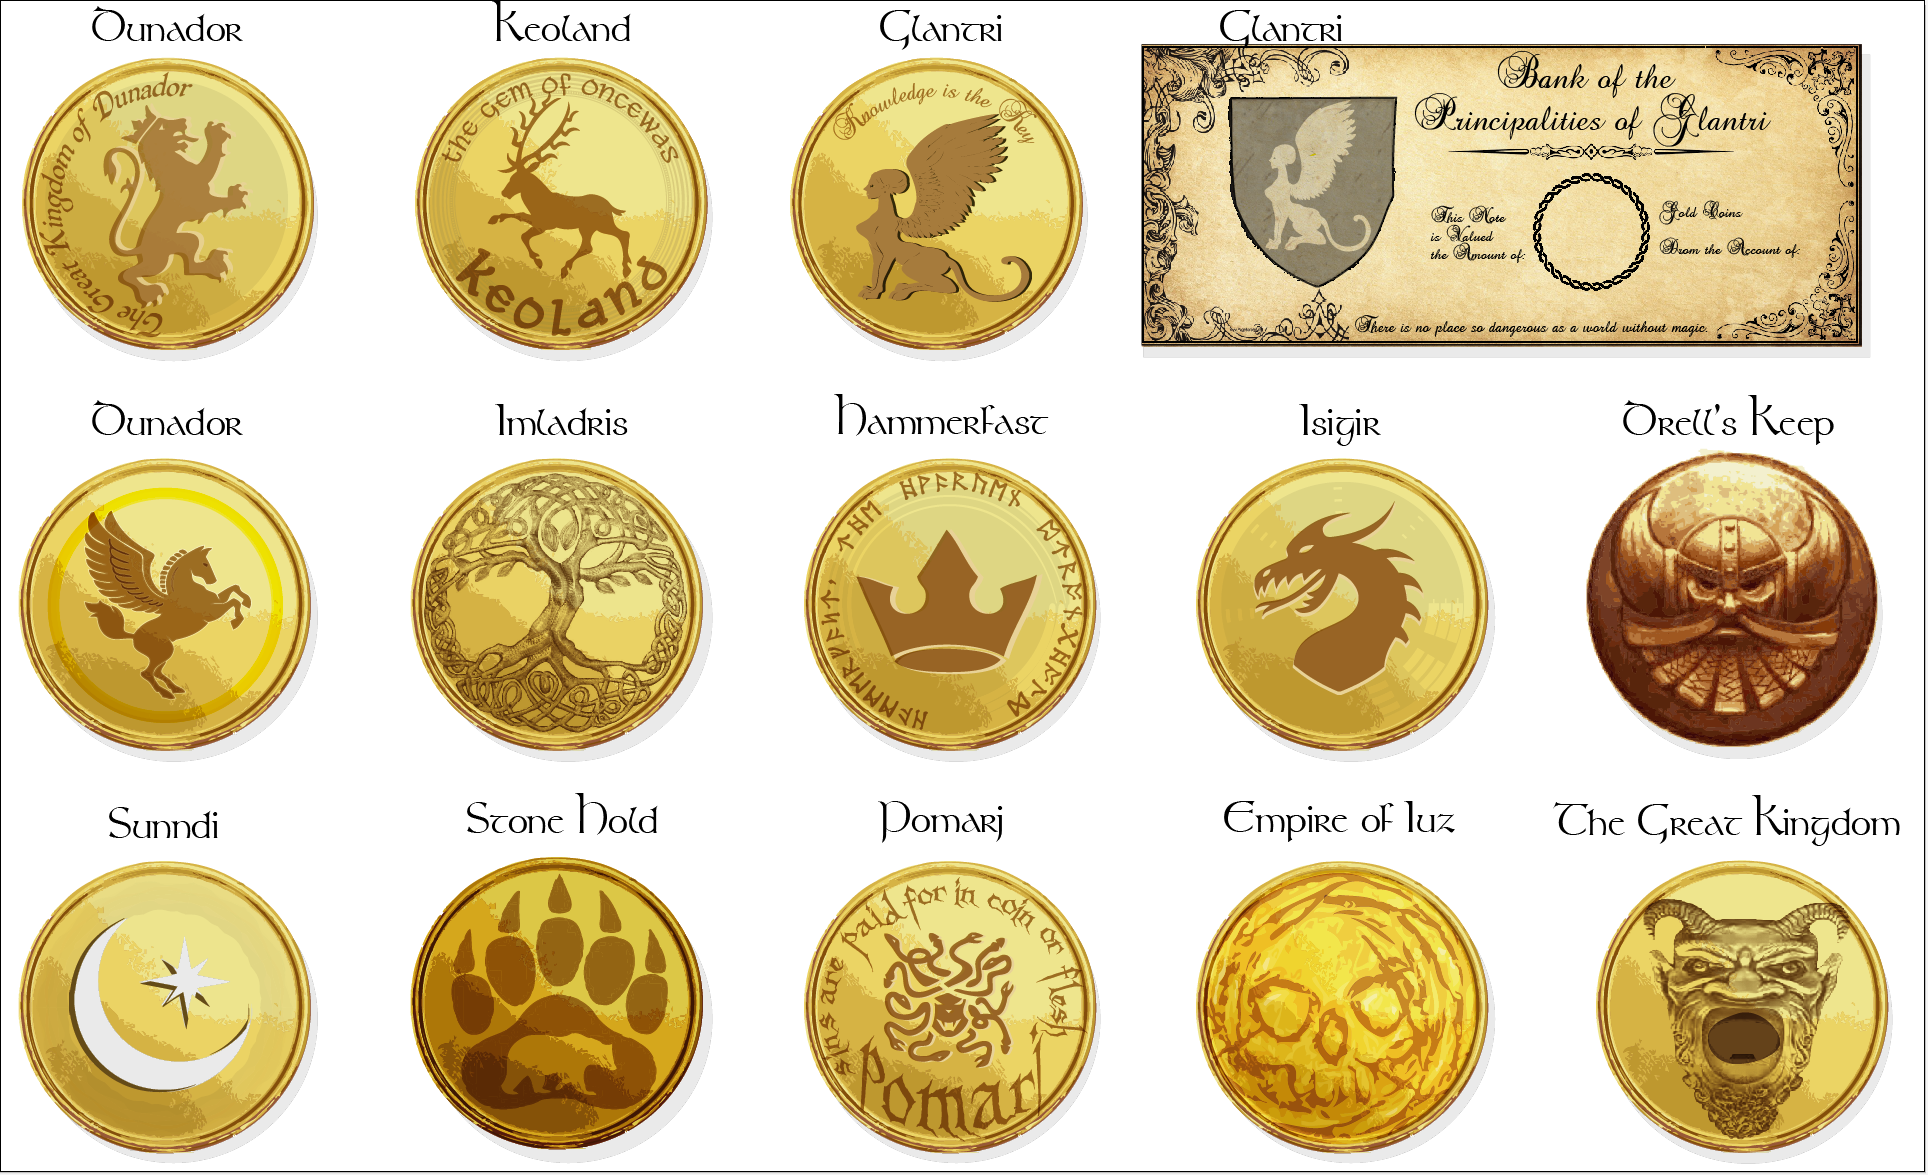
\includegraphics{./images/coins.png}

Monetary values are usually expressed in gold pieces. In addition to
gold coins, there are coins made of platinum, silver, electrum (an alloy
of gold and silver), and copper. They are valued as follows:

1 platinum piece (pp)= 5 gold pieces (gp)

1 gold piece (gp)= 10 silver pieces (sp)

1 electrum piece (ep)= 5 silver pieces (sp)

1 silver piece (sp)= 10 copper pieces (cp)

For game purposes, assume that one gold piece weighs
1/20\textsuperscript{th}~of a pound, and that five coins will ``fit'' in
a cubic inch of storage space (this isn't literally accurate, but works
well enough when applied to a box or chest).

As a reference here is a rough equivalance to modern currency, 1 silver
coin is roughly equal to 1 US dollar. Hence:

\emph{1 pp = \$50. 1 gp = \$10. 1 ep = \$5. 1 sp = \$1. 1 cp = ₵10}

First level characters generally begin the game with 3d6 x 10 gp (unless
the DM decides otherwise).

\begin{Shaded}
\begin{Highlighting}[]
\NormalTok{import \{ generalDice \} from "./custom.js"}

\NormalTok{viewof goldRoll = Inputs.button(html\textasciigrave{}\textless{}button style="color: black; background{-}color: lightgray;"\textgreater{}Roll Starting Gold\textless{}/button\textgreater{}\textasciigrave{}, \{value: 0, reduce: () =\textgreater{} (10 * generalDice(3,6,0))\})}
\end{Highlighting}
\end{Shaded}

\textbf{Starting Gold}: \$\{goldRoll\}

\section{Misc. Equipment}\label{misc.-equipment}

This list represents common adventuring equipment at average prices.
Prices and availability may vary. Weights are expressed in pounds. Items
marked * weigh very little; ten such items weigh one pound. Items marked
** have almost no weight and should not usually be counted.

\begin{longtable}[]{@{}lll@{}}
\toprule\noalign{}
Item & Price & Weight \\
\midrule\noalign{}
\endhead
\bottomrule\noalign{}
\endlastfoot
Backpack & 4 gp & * \\
Belt Pouch & 1 gp & * \\
Bit and bridle & 15 sp & 3 \\
Candles, 12 & 1 gp & * \\
Chalk, small bag of pieces & 2 gp & * \\
Cloak & 2 gp & 1 \\
Clothing, common outfit & 4 gp & 1 \\
Glass bottle or vial & 1 gp & * \\
Grappling Hook & 2 gp & 4 \\
Holy Symbol & 25 gp & * \\
Holy Water, per vial & 10 gp & * \\
Horseshoes \& shoeing & 1 gp & 10 \\
Ink, per jar & 8 gp & ½ \\
Iron Spikes, 12 & 1 gp & 1 \\
Ladder, 10 ft. & 1 gp & 20 \\
Lantern & 5 gp & 2 \\
Lantern, Bullseye & 14 gp & 3 \\
Lantern, Hooded & 8 gp & 2 \\
Manacles (without padlock) & 6 gp & 4 \\
Map or scroll case & 1 gp & ½ \\
Mirror, small metal & 7 gp & * \\
Oil (per flask) & 1 gp & 1 \\
Padlock (with 2 keys) & 12 gp & 1 \\
Paper (per sheet) & 1 gp & ** \\
Pole, 10' wooden & 1 gp & 10 \\
Quill & 1 sp & ** \\
Quill Knife & 1 gp & * \\
Quiver or Bolt case & 1 gp & 1 \\
Rations, Dry, one week & 10 gp & 14 \\
Rope, Hemp (per 50 ft.) & 1 gp & 5 \\
Rope, Silk (per 50 ft.) & 10 gp & 2 \\
Sack, Large & 1 gp & * \\
Sack, Small & 5 sp & * \\
Saddle, Pack & 5 gp & 15 \\
Saddle, Riding & 10 gp & 35 \\
Saddlebags, pair & 4 gp & 7 \\
Spellbook (128 pages) & 25 gp & 1 \\
Tent, Large (ten men) & 25 gp & 20 \\
Tent, Small (one man) & 5 gp & 10 \\
Thieves' picks and tools & 25 gp & 1 \\
Tinderbox, flint and steel & 3 gp & 1 \\
Torches, 6 & 1 gp & 1 \\
Whetstone & 1 gp & 1 \\
Whistle & 1 gp & ** \\
Wineskin/Waterskin & 1 gp & 2 \\
Winter blanket & 1 gp & 3 \\
\end{longtable}

\subsection{Equipment Explanations}\label{equipment-explanations}

A~\textbf{Backpack}~will hold a maximum 40 pounds or 3 cubic feet of
goods. Some items may be lashed to the outside, and thus count toward
the weight limit but not the volume limit. A Halfling's backpack holds
at most 30 pounds and/or 1½ cubic feet, but costs the same as a
full-sized item.

A~\textbf{Candle}~will shed light over a 5' radius, with dim light
extending 5' further. A normal candle will burn about 3 turns per inch
of height.

\textbf{Chalk}~is useful for ``blazing a trail'' through a dungeon or
ruin.

\textbf{Holy Water}~is explained in
the~\hyperref[holy-water]{Encounter~section}.

\textbf{Iron Spikes}~are useful for spiking doors closed (or spiking
them open) and may be used as crude pitons in appropriate situations.

A~\textbf{Lantern}~will provide light covering a 30' radius; dim light
will extend about 20' further. A lantern will consume a flask of oil in
18+1d6 turns. A~\textbf{Hooded Lantern}~allows the light to be hidden or
revealed as the user pleases; in all other ways it performs as an
ordinary lantern. A~\textbf{Bullseye Lantern}~projects a cone of light
30' long and 30' wide at the widest point, with dim light extending an
additional 20' beyond that point. This type of lantern is generally
hooded.

A~\textbf{Map or Scroll Case}~is a tubular oiled leather case used to
carry maps, scrolls, or other paper items. The case will have a
water-resistant (but not waterproof) cap which slides over the end, and
a loop to allow the case to be hung from a belt or bandolier. A standard
scroll case can hold up to 10 sheets of paper, or a single scroll of up
to seven spells.

A~\textbf{Mirror}~is useful in a dungeon environment for many reasons;
for instance, it is the only way to look at a Medusa without being
turned to stone. Mirrors are also useful for looking around corners, and
can be used outdoors to send signals using reflected sunlight.

A~\textbf{Quiver}~is an open container used to hold arrows.
A~\textbf{Bolt Case}~is a similar sort of container for crossbow bolts.
In either case, the standard capacity is 20 missiles. The length of a
quiver or bolt case must match the length of the ammunition for it to be
useful; therefore, there are longbow and shortbow quivers and light and
heavy crossbow bolt cases. The price is the same for all types.

\textbf{Dry Rations}~may consist of dry bread, hard cheese, dried fruit,
nuts, beans, jerky, or any other food which will not ``go bad'' in less
than about a month (if not longer). Dry rations are generally sold in
quantities sufficient for one character for a week, and are packaged in
waxed or oiled cloth to protect them.

\textbf{Hemp Rope}~is ½ inch in diameter and has a breaking strength of
1,600 pounds. Safe working load for a rope is normally one-quarter of
the breaking strength. One or more knots in a rope cut the breaking
strength in half. This does not affect the safe working load, because
knots are figured into the listed one-quarter ratio.

\textbf{Silk Rope}~is about 3/8 inch in diameter and has a breaking
strength of 1,600 pounds, although it weighs considerably less than hemp
rope. The notes regarding rope strength given for hemp rope, above,
apply here also.

A~\textbf{Large Sack}~will hold at most 40 pounds or 4 cubic feet of
goods.

A~\textbf{Small Sack}~will hold at most 20 pounds or 2 cubic feet of
goods.

A pair of~\textbf{Saddlebags}~will hold at most 10 pounds or 1 cubic
foot of goods (divided evenly between both bags).

\textbf{Thieves' Picks and Tools}~are required for the use of Thief
abilities such as opening locks and removing traps. These abilities may
not be usable without appropriate tools, or may be used at a penalty at
the option of the Dungeon Master .

A~\textbf{Tinderbox}~is generally purchased with a~\textbf{flint and
steel}; the flint, a piece of hard rock, is struck vigorously against a
C-shaped piece of high-carbon steel. When done correctly, hot sparks
will fly from the flint and steel into the tinder, hopefully starting a
fire. The best tinder is a dried piece of prepared tinder fungus,
carried in the tinderbox to keep it dry; char cloth, hemp rope, or even
very dry grass can substitute if prepared tinder fungus is not
available. The time required to start a fire should be determined by the
DM according to the prevailing conditions; under ideal conditions,
starting a fire with a flint, steel and tinder takes about a turn.

A~\textbf{Torch}~sheds light over a 30' radius, with dim light extending
about 20' further, and burns for 1d4+4 turns. Of course, a torch is also
useful for setting flammable materials (such as cobwebs or oil) alight.

A~\textbf{Whetstone}~is used to sharpen and maintain edged weapons such
as swords, daggers, and axes.

\textbf{Wineskin/Waterskin}~is a container for drinking water or wine;
though generally water is taken into a dungeon or wilderness
environment. The standard waterskin holds one quart of liquid, which is
the minimum amount required by a normal character in a single day. If
adventuring in the desert or other hot, dry areas, a character may need
as much as ten times this amount. Note that the given 2 pound weight is
for a full skin; an empty skin has negligible weight.

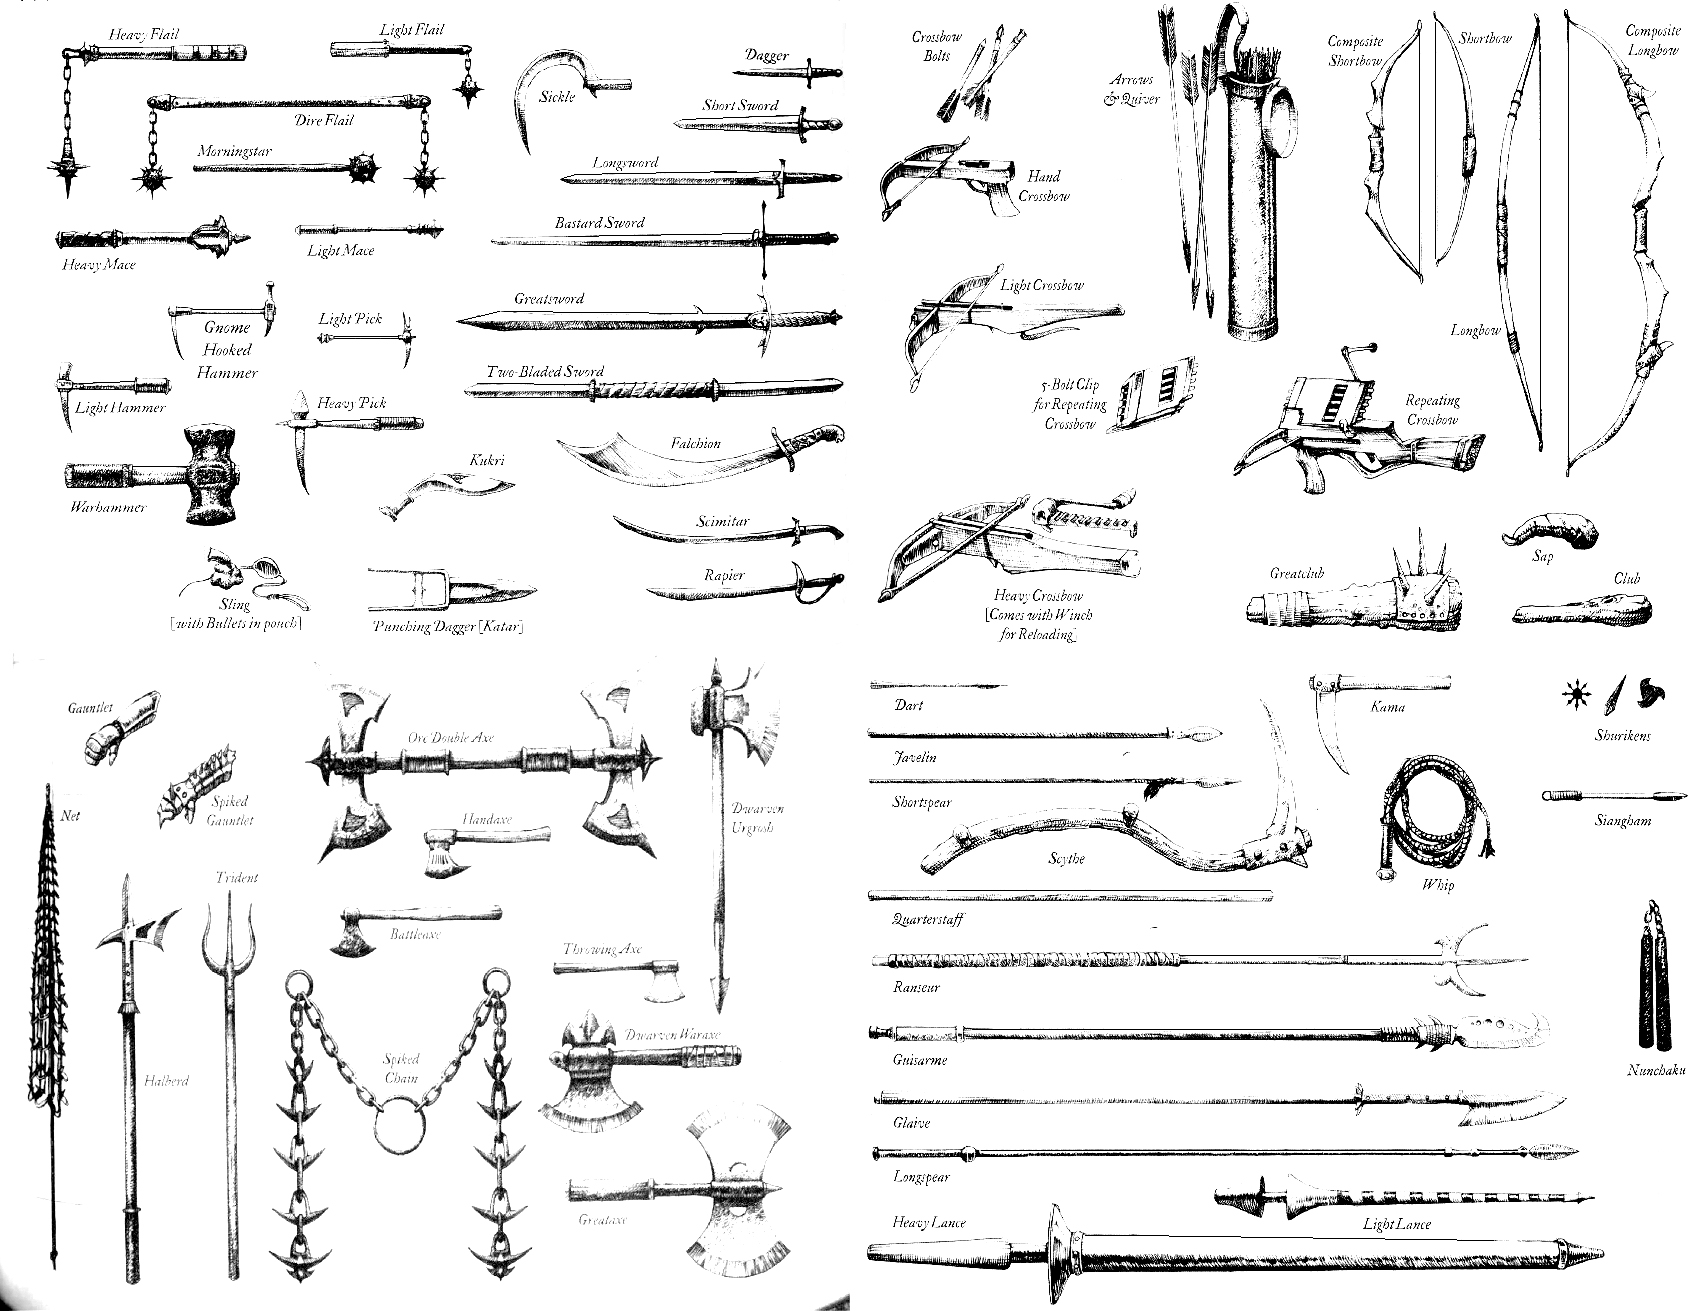
\includegraphics{./images/weapons.jpg}

\section{Weapons}\label{weapons}

\begin{longtable}[]{@{}lllll@{}}
\toprule\noalign{}
Weapon & Price & Size & Weight & Dmg. \\
\midrule\noalign{}
\endhead
\bottomrule\noalign{}
\endlastfoot
\textbf{Axes} & & & & \\
Hand Axe & 4 gp & S & 5 & 1d6 \\
Battle Axe & 7 gp & M & 7 & 1d8 \\
Great Axe & 14 gp & L & 15 & 1d10 \\
\textbf{Bows} & & & & \\
Shortbow & 25 gp & M & 2 & \\
Shortbow Arrow & 1 sp & & * & 1d6 \\
Silver\textsuperscript{†} Shortbow Arrow & 2 gp & & * & 1d6 \\
Longbow & 60 gp & L & 3 & \\
Longbow Arrow & 2 sp & & * & 1d8 \\
Silver\textsuperscript{†} Longbow Arrow & 4 gp & & * & 1d8 \\
Light Crossbow & 30 gp & M & 7 & \\
Light Quarrel & 2 sp & & * & 1d6 \\
Silver\textsuperscript{†} Light Quarrel & 5 gp & & * & 1d6 \\
Heavy Crossbow & 50 gp & L & 14 & \\
Heavy Quarrel & 4 sp & & * & 1d8 \\
Silver\textsuperscript{†} Heavy Quarrel & 10 gp & & * & 1d8 \\
\textbf{Daggers} & & & & \\
Dagger & 2 gp & S & 1 & 1d4 \\
Silver\textsuperscript{†} Dagger & 25 gp & S & 1 & 1d4 \\
\textbf{Swords} & & & & \\
Shortsword & 6 gp & S & 3 & 1d6 \\
Longsword/Scimitar & 10 gp & M & 4 & 1d8 \\
Two-Handed Sword & 18 gp & L & 10 & 1d10 \\
\textbf{Hammers and Maces} & & & & \\
Warhammer & 4 gp & S & 6 & 1d6 \\
Mace & 6 gp & M & 10 & 1d8 \\
Maul & 10 gp & L & 16 & 1d10 \\
\textbf{Other Weapons} & & & & \\
Club/Cudgel/Walking Staff & 2 sp & M & 1 & 1d4 \\
Quarterstaff & 2 gp & L & 4 & 1d6 \\
Pole Arm & 9 gp & L & 15 & 1d10 \\
Sling & 1 gp & S & * & \\
Bullet & 1 sp & & * & 1d4 \\
Stone & n/a & & * & 1d3 \\
Spear & 5 gp & M & 5 & \\
Thrown (one handed) & & & & 1d6 \\
Melee (one handed) & & & & 1d6 \\
Melee (two handed) & & & & 1d8 \\
\end{longtable}

* These items weigh little individually. Ten of these items weigh one
pound.

† Silver tip or blade, for use against lycanthropes

\section{Weapon Size}\label{weapon-size}

\hyperref[humans]{Humans} and \hyperref[elves]{Elves} must wield Large
weapons with both hands, but may use Small or Medium weapons in one
hand. \hyperref[halflings]{Halflings} may not use Large weapons at all,
and must use Medium weapons with both hands.
\hyperref[dwarves]{Dwarves}, due to their stocky, powerful builds, are
able to use Medium weapons one-handed and some Large weapons in two
hands, but Large weapons more than four feet in length are prohibited
(specifically, two-handed swords, polearms, and longbows). Some weapons
must be used with both hands by design (such as bows and crossbows) but
the maximum size limits still apply.

The DM should apply similar limitations to weapon-armed monsters; for
instance, kobolds and goblins are similar in size to Halflings, and thus
should have similar weapon limits.

\section{Missile Weapon Ranges}\label{missile-weapon-ranges}

\begin{longtable}[]{@{}llll@{}}
\toprule\noalign{}
Weapon & Short (+1) & Medium (0) & Long (-2) \\
\midrule\noalign{}
\endhead
\bottomrule\noalign{}
\endlastfoot
Longbow & 70 & 140 & 210 \\
Shortbow & 50 & 100 & 150 \\
Heavy Crossbow & 80 & 160 & 240 \\
Light Crossbow & 60 & 120 & 180 \\
Dagger & 10 & 20 & 30 \\
Hand Axe & 10 & 20 & 30 \\
Oil or Holy Water & 10 & 30 & 50 \\
Sling & 30 & 60 & 90 \\
Spear & 10 & 20 & 30 \\
Warhammer & 10 & 20 & 30 \\
\end{longtable}

Missile weapon ranges are given in feet. In the wilderness, substitute
yards for feet. If the target is as close as or closer than the Short
range figure, the attacker receives a +1 attack bonus. If the target is
further away than the Medium range figure, but not beyond the Long range
figure, the attacker receives a -2 attack penalty.


\includegraphics{images/armor_shields.png}

\section{Armor and Shields}\label{armor-and-shields}

\begin{longtable}[]{@{}llll@{}}
\toprule\noalign{}
Armor Type & Price & Weight & AC \\
\midrule\noalign{}
\endhead
\bottomrule\noalign{}
\endlastfoot
No Armor & 0 gp & 0 & 10 \\
Padded Armor & 15 gp & 10 & 11 \\
Hide & 10 gp & 30 & 12 \\
Leather Armor & 20 gp & 15 & 13 \\
Ring Mail or Studded Leather & 25 gp & 30 & 14 \\
Chain Mail & 60 gp & 40 & 15 \\
Splint Mail & 100 gp & 45 & 16 \\
Plate Mail & 300 gp & 50 & 17 \\
Field Plate & 500 gp & 70 & 18 \\
Full Plate & 1500 gp & 50 & 19 \\
Shield & 7 gp & 8 & +1 \\
\end{longtable}

\emph{Note: that armor for Halfling characters is 50\% heavy as armor
for the other races.}

\section{Beasts of Burden}\label{beasts-of-burden}

Note: Statistics for the animals below are
\hyperref[beasts-of-burden]{here}.

\begin{longtable}[]{@{}ll@{}}
\toprule\noalign{}
Item & Price \\
\midrule\noalign{}
\endhead
\bottomrule\noalign{}
\endlastfoot
Camel & 80 gp \\
Donkey/Mule & 50 gp \\
Horse, Draft & 120 gp \\
Horse, Riding & 75 gp \\
Horse, War & 200 gp \\
Pony* & 50 gp \\
Pony, War* & 80 gp \\
\end{longtable}

*Due to their small stature, Dwarves and Halflings generally ride ponies
rather than horses.

\subsection{War Horse Barding}\label{war-horse-barding}

Barding is armor designed to protect an animal's head, neck, chest, and
body. War Horses and War Ponies are able to wear barding. Studded
Leather, Chain, and Plate armor can be purchased as barding. The cost is
four times the equivalent armor made for humanoids, and it weighs twice
as much.

\begin{longtable}[]{@{}lll@{}}
\toprule\noalign{}
Barding Type & AC & Cost \\
\midrule\noalign{}
\endhead
\bottomrule\noalign{}
\endlastfoot
No Barding & 12 & - \\
Studded Leather Barding & 16 & 100 gp \\
Chain Barding & 17 & 240 gp \\
Plate Barding & 19 & 1200 gp \\
\end{longtable}

\section{Poisons}\label{poisons}


\includegraphics{images/poison.png}

\subsection{Basic Poison}\label{basic-poison}

The first poison must Poisoners learn and easily produced by shadier
folks. This poison is the bread and butter for assassins just starting
out.

This is a contact poison in a thick, reddish liquid form. It somewhat
smells like cucumbers.

Cost: 25 gp per dose

Component: Poisonous Plants

Effect: On a hit, the target takes 1d4 poison damage. Save versus Poison
negates.

Potency: The poison retains potency for 1 minute before drying.

\subsection{Oleander}\label{oleander}

Oleander is a beautiful plant known for its striking flowers. Though
commonly grown as a hedge and ornamental, all parts of the oleander
plant are deadly and contain toxins. If eaten, oleander can cause
vomiting, diarrhea, erratic pulse, seizures, coma, and death, and
contact with the leaves and sap is known to be a skin irritant to some
people. Indeed, the toxins in oleander are so strong that people have
become ill after eating honey made by bees that visited the flowers!
Fortunately, fatalities from oleander poisoning are rare, as the plant
is very bitter and thus quickly deters anyone sampling the vegetation.

Cost: 25 gp per dose

Component: Poisonous Plants

Effect: If ingested, the target takes 1d2 poison damage and is poisoned
for 1d12 hours. A poisoned creature has -1 on Attack rolls, Saving
Throws and Ability Checks. Save versus Poison for half.

Potency: The poison retains potency in food or drink for 2d4 days.

\subsection{Deadly Nightshade}\label{deadly-nightshade}

The sweetness of the berries that often lures children and unwitting
adults to consume this lethal plant. A native of wooded or waste areas
in the OnceWas, deadly nightshade has dull green leaves and shiny black
berries about the size of cherries. Nightshade toxins in its stems,
leaves, berries, and roots causes paralysis in the involuntary muscles
of the body, including the heart. Even physical contact with the leaves
may cause skin irritation.

Cost: 25 gp per dose

Component: Poisonous Plants

Effect: If ingested, the target takes 1d4 dmg. Save versus poison or be
paralyzed for 4d4 hours.

Potency: The poison retains potency in food or drink for 2d4 days.

\subsection{White Snakeroot}\label{white-snakeroot}

White snakeroot is an herb with flat-topped clusters of small white
flowers. Simply drinking the milk of a cow that had grazed on the plant
has poisoned some victims. Indeed, both the meat and milk from poisoned
livestock can pass the toxin to human consumers. Symptoms of ``milk
poisoning'' include loss of appetite, nausea, weakness, abdominal
discomfort, reddened tongue, abnormal acidity of the blood, and death.
Luckily farmers are now aware of this life-threatening hazard and make
efforts remove the plant from animal pastures.

Cost: 25 gp per dose

Component: Poisonous Plants

Effect: If ingested, the target takes 1d4 poison damage and is poisoned
for 2d12 hours. A poisoned creature has -1 on Attack rolls, Saving
Throws and Ability Checks. Save versus Poison for half.

Potency: The poison retains potency in food or drink for 2d4 days.

\subsection{Water Hemlock}\label{water-hemlock}

A large wildflower in the carrot family, water hemlock is sometimes
confused with edible parsnips or celery. The roots are especially toxic,
and will rapidly generate potentially fatal symptoms in anyone unlucky
enough to ingest this poison. Painful convulsions, abdominal cramps,
nausea, and death are common, and those who survive are often afflicted
with amnesia or lasting tremors.

Cost: 25 gp per dose

Component: Poisonous Plants

Effect: If ingested, the target takes 2d4 poison damage and is poisoned
for 24 hours. A poisoned creature has -1 on Attack rolls, Saving Throws
and Ability Checks. Save versus Poison for half.

Potency: The poison retains potency in food or drink for 2d6 weeks..

\subsection{Giant Spider Poison}\label{giant-spider-poison}

This is an ingested Poison in a milky liquid form. It smells pungent and
bitter.

Cost: 50 gp per dose

Component: Giant Poisonous Spiders

Effect: If consumed this poison causes 1d10 hp dmg and parallzation for
2d4 hours. Save for half damage and violent vomiting for 1-4 rounds.

Potency: The poison retains potency in food or drink for 2d6 months.

\subsection{Assassin's Blood}\label{assassins-blood}

An assassin's favorite tool to make the target think they have food
poisoning. This is the best tool to get a target away from a group and
allow them to finish the job.

This is an ingested Poison in a clear liquid form. It faintly smells
like copper.

Cost: 75 gp per dose

Component: Giant Scorpion Venom

Effect: When ingested, the target takes 1d12 poison damage and is
poisoned for 24 hours. A poisoned creature has -1 on Attack rolls,
Saving Throws and Ability Checks.. Save versus Poison for half.

Potency: The poison retains potency for 1 hour when applied to food or
drink.

\subsection{Serpent Venom}\label{serpent-venom}

This poison is harvested from a dead or giant Poisonous Snake.

It is a greasy contact Poison that has an oily sheen.

Cost: 100 gps per dose

Component: Giant Poisonous Snake Venom

Effect: 3d6 poison damage. Save negates.

Potency: This poison stays potent for 24 hours or until delivered
through a wound or washed off.

\subsection{Carrion Crawler Mucus}\label{carrion-crawler-mucus}

One of the odder venoms on the market, this venom is theorized to be
created from the necrotic flesh that Carrion Crawlers regularly devour.

This is a contact poison in a thick, yellow paste. It smells like
rotting garbage.

Cost: 200 gp per dose

Component: Carrion Crawlers Mucus

Effect: On a hit, the target must make a Poison saving throw, they are
poisoned and take 1d4 poison damage on a fail, or half damage on a save.

Aftereffect: If the target fails the initial saving throw, at the start
of their next turn they become paralyzed. At the end of their turn they
can repeat the saving throw, ending the paralyzed and poisoned condition
on a success.

Duration: Target is Poisoned and Paralyzed until they save.

Potency: This poison stays potent for 10 minutes when applied to a
weapon.

\subsection{Essence of Ether}\label{essence-of-ether}

Breathing in this vapor subjects a creatures to its effect. Holding
one's breath is ineffective against inhaled poisons, as they affect
nasal membranes, tear ducts, and other parts of the body. A creature
subjected to this poison must succeed on a poison saving throw with a -1
penalty or become unconscious.

This poison is a pleasant-smelling colorless inhaled vapor.

Cost: 250 gps

Component: This is a mysterious Alchemist concoction

Effect: The poisoned creature is unconscious. The creature awakens if
they take damage or if another creature spends an action to awaken them.

Duration: 8 hours

Potency: Dissipates in 1d4 rounds

\subsection{Malice}\label{malice}

Malice is a white, odorless, bitter crystalline powder that is blown
into the eyes or inhaled by the victim.

Cost: 300 gps per dose

Component:

Effect: A creature subjected to this poison must succeed on a Poison
saving throw or become blinded for 1 hour.

Duration: 1 hour.

Potency: Dissipates immediately.

\subsection{Pale Tincture}\label{pale-tincture}

This strange substance is harvested from fungi cultivated by Myconids in
their lairs under ground. The poison is extracted by squeezing the
liquid out of the Pale mushrooms.

This pale tan liquid is an ingested poison with an earthy smell.

Cost: 400 gp per dose

Component: Fungi cultivated by Myconids

Effect: A creature subjected to this poison must make a Poison saving
throw or take 1d6 poison damage

and become poisoned.

Aftereffects: The poisoned creature must repeat the saving throw every
24 hours, taking 1d6 poison damage on a failed save.

Duration: Target is poisoned until they succeed on seven saving throws
against the poison.

Potency: This poison stays potent for 1 hour when applied to food or
drink.

\subsection{Burnt Othur Fumes}\label{burnt-othur-fumes}

This mist is sprayed out into a 5 foot cube and burns through the
membranes of nasal passageways and through the soft tissue of the mouth.
This lingering poison is designed to kill quickly before its affects can
be stopped.

This is sprayed mist that smells like burning dust.

Cost: 500 gp per dose

Component: Giant Wasp Venom

Effect: A creature subjected to this must succeed on a saving throw
against poison or take 3d6 poison damage and must repeat the saving
throw at the start of each of its turns.

Aftereffect: On each successive failed save, the character takes 3 (1d6)
poison damage. After three successful saves, the poison ends.

Duration: Target must make three successful saves.

Potency: Dissipates immediately.

\subsection{Drow Sleep Poison}\label{drow-sleep-poison}

This poison is said to be made only by the drow, and only in a place far
removed from sunlight. The Drow Sleep Poison is a contact poison that is
a black, gummy, and heavy substance similar to molasses.

Cost: 600 gps per dose

Component: Drow poisonmakers extract this toxin from a slippery, black
fungus that grows like great slicks of oil in the Vault.

Effect: Unconsciousness for 4d6 hours. A successful Save negates
unconsciousness but the creature suffers a -2 penalty to Attack, Saving
throws, and Ability Checks for 2d6 hours.

Potency: The poison retains potency for 2 hours when applied to a
weapon. Sunlight reduces the potency by half.

\subsection{Wyvern Poison}\label{wyvern-poison}

This venom comes from the vicious wyvern. Many have died trying to
harvest this venom as it the tail of the wyvern will occasionally jab
out with muscle spasms, even in death.

Wyvern Poison is a thick, amber colored contact poison.

Cost: 1200 gp per dose

Component: Wyvern Stinger Poison

Effect: On a hit, the target must make a saving throw, taking 7d6 poison
damage on a fail, or half as much on a successful save.

Potency: Stays potent until delivered through a wound or washed off.

\subsection{Midnight Tears}\label{midnight-tears}

A creature that ingests this poison suffers no Effect until the stroke
of midnight. If the poison has not been neutralized before then, the
creature must succeed on a poison throw, taking 9d6 poison damage on a
failed save, or half as much damage on a successful one.

A clear, odorless and colorless liquid, it only reveals itself as an
inky black poison when it comes into contact with cold iron.

Cost: 1500 gps per dose

Component: Rare black flowers that bloom at midnight in the Grey Lands.

Effect: The poisoned creature is unconscious. The creature awakens they
take damage or if another creature spends an action to awaken them.

Duration: 8 hours

Potency: Dissipates immediately

\subsection{Purple Worm Poison}\label{purple-worm-poison}

From the stingers of a Purple Worm, this powerful poison is also used in
alcoholic beverages to provide a powerful kick, not for the feint of
heart.

This is a gooey purplish contact poison that has a sharp smell to it
that burns the nostrils.

Cost: 2000 gp per dose

Component: Purple Worm Stingers

Effect: On a hit, the target must make a Poison saving throw, taking
12d6 poison damage on a fail, or half as much on a successful save.

Potency: Stays potent until delivered through a wound or washed off.

\section{Clerical Spell Costs}\label{clerical-spell-costs}

\subsection{Seeking Divine Aid}\label{seeking-divine-aid}

It is often possible to seek divine aid in the form of clerical spells
from temples dedicated to one of the 12 gods of OnceWas. The
availability and cost may vary depending on the specific god's temple,
the region, and the cleric's willingness to perform the spell. Some
temples may also require a quest or service in addition to the monetary
cost. It is recommended to inquire at multiple temples and be prepared
for potential additional requirements or variations in pricing.

\textbf{0 Level Spell} - 50 gp\\
\emph{Example: Cure Minor Wounds}

\textbf{1st Level Spell} (Adept, minimum 2nd level cleric) - 100 gp\\
\emph{Example: Cure Light Wounds}

\textbf{2nd Level Spell} (Vicar, minimum 4th level cleric) - 200 gp\\
\emph{Example: Restore Health (level 2) - 50 gp}

\textbf{3rd Level Spell} (Curate, minimum 6th level cleric) - 500 gp\\
\emph{Examples: Cure Blindness, Cure Deafness, Cure Disease, Remove
Curse}

\textbf{4th Level Spell} (High Priest, minimum 8th level cleric) - 1000
gp\\
\emph{Example: Cure Serious Wounds}

\textbf{5th Level Spell} (High Priest, minimum 10th level cleric) -
10,000 gp\\
\emph{Example: Raise Dead}

\textbf{6th Level Spell} (Bishop, 12th level cleric) - 20,000 gp\\
\emph{Example: Restoration}

\textbf{7th Level Spell} (Patriarch, minimum 14th level cleric) - 50,000
gp\\
\emph{Example: Resurrection}

\chapter{Vehicles}\label{vehicles}

The following tables give details of various land and sea vehicles. Game
Masters should feel free to create their own vehicles, in which case the
table can be used for guidance. Some of the statistics given below are
explained in detail later.

\section{Land Transportation}\label{land-transportation}

\begin{figure*}

\begin{longtable}[]{@{}
  >{\raggedright\arraybackslash}p{(\columnwidth - 12\tabcolsep) * \real{0.1169}}
  >{\raggedright\arraybackslash}p{(\columnwidth - 12\tabcolsep) * \real{0.2208}}
  >{\raggedright\arraybackslash}p{(\columnwidth - 12\tabcolsep) * \real{0.1039}}
  >{\raggedright\arraybackslash}p{(\columnwidth - 12\tabcolsep) * \real{0.0909}}
  >{\raggedright\arraybackslash}p{(\columnwidth - 12\tabcolsep) * \real{0.1299}}
  >{\raggedright\arraybackslash}p{(\columnwidth - 12\tabcolsep) * \real{0.1948}}
  >{\raggedright\arraybackslash}p{(\columnwidth - 12\tabcolsep) * \real{0.1429}}@{}}
\toprule\noalign{}
\begin{minipage}[b]{\linewidth}\raggedright
Vehicle
\end{minipage} & \begin{minipage}[b]{\linewidth}\raggedright
Length x width*
\end{minipage} & \begin{minipage}[b]{\linewidth}\raggedright
Weight
\end{minipage} & \begin{minipage}[b]{\linewidth}\raggedright
Cargo
\end{minipage} & \begin{minipage}[b]{\linewidth}\raggedright
Movement
\end{minipage} & \begin{minipage}[b]{\linewidth}\raggedright
Hardness / HP
\end{minipage} & \begin{minipage}[b]{\linewidth}\raggedright
Cost (gp)
\end{minipage} \\
\midrule\noalign{}
\endhead
\bottomrule\noalign{}
\endlastfoot
Chariot & 15' x 6' & 300 & 750 lbs & 60' (10') & 10 / 10 & 400 \\
Coach & 30' x 8' & 1,000 & 2,000 lbs & 40' (15') & 6 / 12 & 1,500 \\
Wagon & 35' x 8' & 2,000 & 4,000 lbs & 20' (15') & 6 / 16 & 500 \\
\end{longtable}

\end{figure*}%

*Includes hitched horses or mules.

\section{Water Transportation}\label{water-transportation}

\begin{figure*}

\begin{longtable}[]{@{}
  >{\raggedright\arraybackslash}p{(\columnwidth - 14\tabcolsep) * \real{0.1562}}
  >{\raggedright\arraybackslash}p{(\columnwidth - 14\tabcolsep) * \real{0.1667}}
  >{\raggedright\arraybackslash}p{(\columnwidth - 14\tabcolsep) * \real{0.1042}}
  >{\raggedright\arraybackslash}p{(\columnwidth - 14\tabcolsep) * \real{0.0625}}
  >{\raggedright\arraybackslash}p{(\columnwidth - 14\tabcolsep) * \real{0.1250}}
  >{\raggedright\arraybackslash}p{(\columnwidth - 14\tabcolsep) * \real{0.1146}}
  >{\raggedright\arraybackslash}p{(\columnwidth - 14\tabcolsep) * \real{0.1562}}
  >{\raggedright\arraybackslash}p{(\columnwidth - 14\tabcolsep) * \real{0.1146}}@{}}
\toprule\noalign{}
\begin{minipage}[b]{\linewidth}\raggedright
Vehicle
\end{minipage} & \begin{minipage}[b]{\linewidth}\raggedright
Length x Width
\end{minipage} & \begin{minipage}[b]{\linewidth}\raggedright
Cargo
\end{minipage} & \begin{minipage}[b]{\linewidth}\raggedright
Crew
\end{minipage} & \begin{minipage}[b]{\linewidth}\raggedright
Movement
\end{minipage} & \begin{minipage}[b]{\linewidth}\raggedright
Miles/Day
\end{minipage} & \begin{minipage}[b]{\linewidth}\raggedright
Hardness / HP
\end{minipage} & \begin{minipage}[b]{\linewidth}\raggedright
Cost (gp)
\end{minipage} \\
\midrule\noalign{}
\endhead
\bottomrule\noalign{}
\endlastfoot
Canoe & 15' x 4' & ½ ton & 1 & 40' (5') & 30 & 4 / 4 & 50 \\
Caravel & 55' x 15' & 75 tons & 10 & 20' (20') & 42 & 8 / 75 & 10,000 \\
Carrack & 60' x 20' & 135 tons & 20 & 30' (30') & 48 & 10 / 120 &
20,000 \\
Galley, Small & 100' x 15' & 210 tons & 90 & 20' (20') & 36 / 24 & 8 /
75 & 15,000 \\
Galley, Large & 120' x 20' & 375 tons & 160 & 30' (25') & 42 / 24 & 10 /
120 & 30,000 \\
Longship & 110' x 15' & 10 tons & 70 & 30' (25') & 42 / 24 & 9 / 110 &
25,000 \\
Raft/Barge & per 10' x 10' & 1 ton & 2 & 40' (10') & 18 & 6 / 12 &
100 \\
Riverboat & 50' x 20' & 50 tons & 10 & 20' (20') & 30 & 8 / 30 &
3,500 \\
Rowboat & 15' x 6' & 1 ton & 1 & 30' (10') & 24 & 6 / 8 & 60 \\
Sailboat & 40' x 8' & 5 tons & 1 & 40' (15') & 36 & 7 / 20 & 2,000 \\
\end{longtable}

\end{figure*}%

\section{Notes Regarding Vehicles}\label{notes-regarding-vehicles}

The\textbf{~Crew}~figure given reflects the minimum number of sailors
and/or rowers needed to operate the ship. Officers are not counted among
these numbers, and of course it is always a good idea to hire extra
sailors and/or rowers to ensure that any casualties will not slow down
the ship.

\textbf{Cargo}~for wagons is given in pounds, while for ships it is
given in tons. If the ship sails night and day, each passenger requires
living space equivalent to one ton of cargo; in addition, provisions for
one man for one month occupy 1/10 of a ton of space.

\textbf{Movement}~is given separately here in feet (yards, actually;
see~\hyperref[time-and-scale]{Time and Scale}~for an explanation) as
well as miles per day. The encounter movement of ships is not directly
related to the long-distance travel rate, since the crew must work hard
to make the ship move quickly in combat, and this level of effort cannot
be maintained day and night.

The parenthesized figure represents maneuverability;
see~\textbf{Maneuverability}~in~\textbf{Part 5: The Encounter}~for
details.

See~\textbf{Attacking a Vehicle,}~also in
the~\hyperref[maneuverability]{Encounter}~section, for details on
the~\textbf{Hardness}~and~\textbf{HP}~statistics.

A~\textbf{chariot}~requires a single horse, generally a warhorse, to
pull it. Both~\textbf{coaches}~and\textbf{~wagons}~require at least a
pair of draft horses to pull them.

A~\textbf{caravel}~is a highly maneuverable sailing ship with two or
three masts. Though superficially similar to the larger carrack,
caravels are capable of sailing up rivers, a task for which the larger
ship is ill suited.

A~\textbf{carrack}~is a large, ocean-going sailing ship with three or
four masts.

\textbf{Galleys}~are equipped with both sails and oars; the second
listed movement rate for galleys is the rowing speed. A small galley
will have around 20 rows of oars, with each oar pulled by two men (for a
total of 80 rowers) while a large galley will have around 35 rows of
oars (for a total of 140 rowers). Galleys are generally much more
maneuverable than sailing ships such as the carrack or caravel, and may
be outfitted with rams.

The~\textbf{longship}~commonly used by northern raiders is very similar
to the large galley. However, where more civilized nations have
specialist rowers, sailors, and marines, the crew of a longship is more
generalized; most crewmen will be qualified for all of these tasks.

\section{Siege Engines}\label{siege-engines}

These are weapons used to attack strongholds, or sometimes ships. Their
cost may be up to twice as high in a remote location. A siege engine
that throws missiles (a ballista, onager or trebuchet) must have a
trained artillerist to fire it; this is the character who makes the
attack rolls for the weapon. Missile-throwing engines have attack
penalties, detailed below. Note: siege engines are not generally usable
against individuals or monsters; the DM may make exceptions for very
large monsters like giants or dragons. Review the rules in the
\hyperref[strongholds]{Stronghold} section for details regarding
attacking fortified buildings such as castles, towers, fortresses, and
so on.

\begin{figure*}

\begin{longtable}[]{@{}
  >{\raggedright\arraybackslash}p{(\columnwidth - 14\tabcolsep) * \real{0.1250}}
  >{\raggedright\arraybackslash}p{(\columnwidth - 14\tabcolsep) * \real{0.1250}}
  >{\raggedright\arraybackslash}p{(\columnwidth - 14\tabcolsep) * \real{0.1250}}
  >{\raggedright\arraybackslash}p{(\columnwidth - 14\tabcolsep) * \real{0.1250}}
  >{\raggedright\arraybackslash}p{(\columnwidth - 14\tabcolsep) * \real{0.1250}}
  >{\raggedright\arraybackslash}p{(\columnwidth - 14\tabcolsep) * \real{0.1250}}
  >{\raggedright\arraybackslash}p{(\columnwidth - 14\tabcolsep) * \real{0.1250}}
  >{\raggedright\arraybackslash}p{(\columnwidth - 14\tabcolsep) * \real{0.1250}}@{}}
\toprule\noalign{}
\begin{minipage}[b]{\linewidth}\raggedright
Weapon
\end{minipage} & \begin{minipage}[b]{\linewidth}\raggedright
Cost
\end{minipage} & \begin{minipage}[b]{\linewidth}\raggedright
Rate of Fire
\end{minipage} & \begin{minipage}[b]{\linewidth}\raggedright
Attack Penalty
\end{minipage} & \begin{minipage}[b]{\linewidth}\raggedright
Damage
\end{minipage} & \begin{minipage}[b]{\linewidth}\raggedright
Short Range (+1)
\end{minipage} & \begin{minipage}[b]{\linewidth}\raggedright
Medium Range (+0)
\end{minipage} & \begin{minipage}[b]{\linewidth}\raggedright
Long Range (-2)
\end{minipage} \\
\midrule\noalign{}
\endhead
\bottomrule\noalign{}
\endlastfoot
Ballista & 100 gp & 1/4 & -3 & 2d8 & 50' & 100' & 150' \\
Battering Ram & 200 gp & 1/3 & +0 & 2d8 & N/A & N/A & N/A \\
Onager & 300 gp & 1/6 & -6 & 2d12 & 100' & 200' & 300' \\
Screw & 200 gp & N/A & N/A & 1d8 & N/A & N/A & N/A \\
Sow & 100 gp & N/A & N/A & N/A & N/A & N/A & N/A \\
Trebuchet & 400 gp & 1/10 & -8 & 3d10 & N/A & 300' & 400' \\
\end{longtable}

\end{figure*}%

\textbf{Ballista:}~This is effectively a very large crossbow that may
fire a spear-like bolt or a large stone. It is usually mounted on a
tripod or wagon, but may also be mounted on a ship. When firing bolts, a
ballista cannot damage brick or stone. A ballista requires a crew of
three to operate.

\textbf{Battering Ram:}~These are usually operated under a sow (a sort
of portable roof). They require a crew of eight or more.

\textbf{Onager:}~This weapon throws a stone with a fairly flat
trajectory. An onager requires a crew of four to operate.

\textbf{Screw}: This device may be used to attack a stronghold, by means
of boring through the walls. A crew of at least eight is required to
operate it. It is only used at the base of a wall, and it is usually
operated under a sow.

\textbf{Sow}: This is a kind of portable roof, used for protection while
performing slower attacks on a fortified building. Those under a sow
will be harder to hit, receiving at least a +6 bonus to Armor Class
against ranged attacks while taking cover under it. The sow itself has a
hardness of 9 and 50 hit points.

\textbf{Trebuchet:}~This mighty weapon uses a counterweight to fling a
stone on a high, arcing path. It cannot fire at targets within 200
yards. If it is aimed at a target that is more than 20' higher than the
weapon, there is an additional --2 attack penalty. A trebuchet requires
a crew of eight to operate.

\part{Magic}

\chapter{Spells}\label{spells}

The number of spells of each level which a Cleric or Magic-User may cast
per day is shown on the appropriate table in
the~\hyperref[character-classes]{Classes}~section. Each day, usually in
the morning, spellcasters prepare spells to replace those they have
used. Clerics do this through prayer, while Magic-Users must study their
spellbooks. Spells prepared but not used persist from day to day; only
those actually cast must be replaced. A spellcaster may always choose to
dismiss a prepared spell (without casting it) in order to prepare a
different spell of that level.

Spellcasters must have at least one hand free, and be able to speak, in
order to cast spells; thus, binding and gagging a spellcaster is an
effective means of preventing him or her from casting spells. In combat,
casting a spell usually takes the same time as making an attack. If a
spellcaster is attacked (even if not hit) or must make a saving throw
(whether successful or not) on the Initiative number on which he or she
is casting a spell, the spell is spoiled and lost. As a specific
exception, two spell casters releasing their spells at each other on the
same Initiative number will both succeed in their casting; one caster
may disrupt another with a spell only if he or she has a better
Initiative, and chooses to delay casting the spell until~\emph{right
before}~the other caster.

Some spells are reversible; such spells are shown with an asterisk after
the name.

\chapter{Cleric Spells}\label{cleric-spells}

Clerics receive their spells through faith and prayer. Each day,
generally in the morning, a Cleric must pray for at least three turns in
order to prepare spells. Of course, the Cleric may be expected to pray
more than this in order to remain in his or her deity's good graces.

Because they gain their spells through prayer, a Cleric may prepare any
spell of any level he or she is able to cast. However, in some cases the
Cleric's deity may limit the availability of certain spells; for
instance, a deity devoted to healing may refuse to grant reversed
healing spells.

\begin{tcolorbox}[enhanced jigsaw, bottomtitle=1mm, coltitle=black, breakable, arc=.35mm, colback=white, colbacktitle=quarto-callout-tip-color!10!white, title={Level 0, Clerical (Orisons)}, rightrule=.15mm, opacitybacktitle=0.6, toptitle=1mm, leftrule=.75mm, colframe=quarto-callout-tip-color-frame, titlerule=0mm, left=2mm, toprule=.15mm, bottomrule=.15mm, opacityback=0]

\begin{tcolorbox}[enhanced jigsaw, bottomtitle=1mm, coltitle=black, breakable, arc=.35mm, colback=white, colbacktitle=quarto-callout-note-color!10!white, title={Cure Minor Wounds*}, rightrule=.15mm, opacitybacktitle=0.6, toptitle=1mm, leftrule=.75mm, colframe=quarto-callout-note-color-frame, titlerule=0mm, left=2mm, toprule=.15mm, bottomrule=.15mm, opacityback=0]

Cleric 0, Druid 0

Range: Touch

Duration: Instantaneous

With this spell the caster heals 1 hit points of damage by laying his or
her hand upon the injured creature.

The reverse form of this spell,~\textbf{Cause Minor Wounds}, causes 1
damage to the creature affected by it. A successful attack roll is
required in this case.

Undead are affected by this spell and its reverse in opposite fashion;
they are injured by~\textbf{Cure Minor Wounds}~and healed
by~\textbf{Cause Minor Wounds}.

\end{tcolorbox}

\begin{tcolorbox}[enhanced jigsaw, bottomtitle=1mm, coltitle=black, breakable, arc=.35mm, colback=white, colbacktitle=quarto-callout-note-color!10!white, title={Dowse}, rightrule=.15mm, opacitybacktitle=0.6, toptitle=1mm, leftrule=.75mm, colframe=quarto-callout-note-color-frame, titlerule=0mm, left=2mm, toprule=.15mm, bottomrule=.15mm, opacityback=0]

Cleric 0, Druid 0

Range: Self

Duration: Contcentration

This minor magical effect allows the caster to sense the presence of
potable water using a forked stick (any will do, but some have
favorites). While outdoors the dowsing rod will twist to point in the
direction of such fresh water up to 1000 feet +100' per level of the
caster. Water that is underground, in containers, or within structures
can be located within 25 feet +5' per level. The effect lasts as long as
the caster maintains concentration.

\end{tcolorbox}

\begin{tcolorbox}[enhanced jigsaw, bottomtitle=1mm, coltitle=black, breakable, arc=.35mm, colback=white, colbacktitle=quarto-callout-note-color!10!white, title={Guidance*}, rightrule=.15mm, opacitybacktitle=0.6, toptitle=1mm, leftrule=.75mm, colframe=quarto-callout-note-color-frame, titlerule=0mm, left=2mm, toprule=.15mm, bottomrule=.15mm, opacityback=0]

Cleric 0, Druid 0

Range: 10'

Duration: Instantaneous

The cleric grants +1 to any subject's next attack roll. Reversed, this
becomes \textbf{Misguide}, which gives the subject -1 to their next
attack roll.

\end{tcolorbox}

\begin{tcolorbox}[enhanced jigsaw, bottomtitle=1mm, coltitle=black, breakable, arc=.35mm, colback=white, colbacktitle=quarto-callout-note-color!10!white, title={Hallow*}, rightrule=.15mm, opacitybacktitle=0.6, toptitle=1mm, leftrule=.75mm, colframe=quarto-callout-note-color-frame, titlerule=0mm, left=2mm, toprule=.15mm, bottomrule=.15mm, opacityback=0]

Cleric 0, Druid

Range: Self

Duration: Instantaneous

By chanting holy phrases, the caster makes the 0 foot radius area around
him `hallowed', granting +1 bonus on Healing spells and Turning
attempts. The effect continues as long as the caster maintains the
chant, but any action other than moving and defending oneself ends the
effect. However, the effect lasts one additional round after the chant
ends, giving the caster the option to cast or turn once and enjoy the
effect himself.

The reverse, \textbf{Unhallow}, works in the same manner by granting +1
damage on Inflict spells (reversed healing) makes undead (or vile
netherworld inhabitants) harder to Turn by one point (or optionally
easier to Command by one point). It likewise lasts one round longer than
the chant is maintained.

\end{tcolorbox}

\begin{tcolorbox}[enhanced jigsaw, bottomtitle=1mm, coltitle=black, breakable, arc=.35mm, colback=white, colbacktitle=quarto-callout-note-color!10!white, title={Meal Blessing}, rightrule=.15mm, opacitybacktitle=0.6, toptitle=1mm, leftrule=.75mm, colframe=quarto-callout-note-color-frame, titlerule=0mm, left=2mm, toprule=.15mm, bottomrule=.15mm, opacityback=0]

Cleric 0, Druid 0

Range: 10'

Duration: Instaneous

The cleric says this short prayer before a meal to give the diners a
blessing. Anyone who eats the meal within twenty minutes heals 1 hit
point. The meal must be normally prepared and obtained in a way that the
deity permits.

\end{tcolorbox}

\begin{tcolorbox}[enhanced jigsaw, bottomtitle=1mm, coltitle=black, breakable, arc=.35mm, colback=white, colbacktitle=quarto-callout-note-color!10!white, title={Mend}, rightrule=.15mm, opacitybacktitle=0.6, toptitle=1mm, leftrule=.75mm, colframe=quarto-callout-note-color-frame, titlerule=0mm, left=2mm, toprule=.15mm, bottomrule=.15mm, opacityback=0]

Cleric 0, Druid 0

Range: 10'

Duration: Instantaneous

Mends breaks, dents, and holes in small objects.

\end{tcolorbox}

\begin{tcolorbox}[enhanced jigsaw, bottomtitle=1mm, coltitle=black, breakable, arc=.35mm, colback=white, colbacktitle=quarto-callout-note-color!10!white, title={Predict Weather}, rightrule=.15mm, opacitybacktitle=0.6, toptitle=1mm, leftrule=.75mm, colframe=quarto-callout-note-color-frame, titlerule=0mm, left=2mm, toprule=.15mm, bottomrule=.15mm, opacityback=0]

Cleric 0, Druid 0

Range: General surroundings

Duration: Instantaneous

The caster may accurately predict the weather up to 24 hours in advance.

\end{tcolorbox}

\begin{tcolorbox}[enhanced jigsaw, bottomtitle=1mm, coltitle=black, breakable, arc=.35mm, colback=white, colbacktitle=quarto-callout-note-color!10!white, title={Virtue}, rightrule=.15mm, opacitybacktitle=0.6, toptitle=1mm, leftrule=.75mm, colframe=quarto-callout-note-color-frame, titlerule=0mm, left=2mm, toprule=.15mm, bottomrule=.15mm, opacityback=0]

Cleric 0, Druid 0

Range: 10'

Duration: 1 round

A subject gains one temporary hit point for ten minutes.

\end{tcolorbox}

\begin{tcolorbox}[enhanced jigsaw, bottomtitle=1mm, coltitle=black, breakable, arc=.35mm, colback=white, colbacktitle=quarto-callout-note-color!10!white, title={Ward*}, rightrule=.15mm, opacitybacktitle=0.6, toptitle=1mm, leftrule=.75mm, colframe=quarto-callout-note-color-frame, titlerule=0mm, left=2mm, toprule=.15mm, bottomrule=.15mm, opacityback=0]

Cleric 0, Druid 0

Range: 10'

Duration: Instantaneous

Grants +1 to the subject's next saving throw. Reversed, this becomes
\textbf{Curse}, which gives the opposite effect.

\end{tcolorbox}

\begin{tcolorbox}[enhanced jigsaw, bottomtitle=1mm, coltitle=black, breakable, arc=.35mm, colback=white, colbacktitle=quarto-callout-note-color!10!white, title={Water to Wine*}, rightrule=.15mm, opacitybacktitle=0.6, toptitle=1mm, leftrule=.75mm, colframe=quarto-callout-note-color-frame, titlerule=0mm, left=2mm, toprule=.15mm, bottomrule=.15mm, opacityback=0]

Cleric 0, Druid 0

Range: 10'

Duration: Instantaneous

The cleric may turn one flask or mug of water to wine. The reverse
\textbf{Wine to Water} turns a flask of wine to pure water.

\end{tcolorbox}

\end{tcolorbox}

\begin{tcolorbox}[enhanced jigsaw, bottomtitle=1mm, coltitle=black, breakable, arc=.35mm, colback=white, colbacktitle=quarto-callout-tip-color!10!white, title={Level 1, Clerical}, rightrule=.15mm, opacitybacktitle=0.6, toptitle=1mm, leftrule=.75mm, colframe=quarto-callout-tip-color-frame, titlerule=0mm, left=2mm, toprule=.15mm, bottomrule=.15mm, opacityback=0]

\begin{tcolorbox}[enhanced jigsaw, bottomtitle=1mm, coltitle=black, breakable, arc=.35mm, colback=white, colbacktitle=quarto-callout-note-color!10!white, title={Command}, rightrule=.15mm, opacitybacktitle=0.6, toptitle=1mm, leftrule=.75mm, colframe=quarto-callout-note-color-frame, titlerule=0mm, left=2mm, toprule=.15mm, bottomrule=.15mm, opacityback=0]

Cleric 1

Range: 10'

Duration: 1 round

The caster speaks a single-word command, which will be obeyed by a
single creature within the given range. The command must be given in a
language the recipient understands. The recipient will do its best to
obey, as long as the command is a clear, imperative verb. ``Suicide''
isn't a verb. ``Die'' would cause the recipient to fake death for the
duration of the spell (believing it was dead). Typical commands are
back, halt, flee, run, stop, fall, fly, go, leave, surrender, sleep,
rest, etc.

Undead are not affected. Creatures with Intelligence of 13 or more and
creatures with 6 or more hit dice may save vs.~Spells to resist.

\end{tcolorbox}

\begin{tcolorbox}[enhanced jigsaw, bottomtitle=1mm, coltitle=black, breakable, arc=.35mm, colback=white, colbacktitle=quarto-callout-note-color!10!white, title={Cure Light Wounds*}, rightrule=.15mm, opacitybacktitle=0.6, toptitle=1mm, leftrule=.75mm, colframe=quarto-callout-note-color-frame, titlerule=0mm, left=2mm, toprule=.15mm, bottomrule=.15mm, opacityback=0]

Cleric 1, Druid 1

Range: Touch

Duration: Instantaneous

With this spell the caster heals 1d6+1 hit points of damage by laying
his or her hand upon the injured creature.

The reverse form of this spell,~\textbf{Cause Light Wounds}, causes
1d6+1 damage to the creature affected by it. A successful attack roll is
required in this case.

Undead are affected by this spell and its reverse in opposite fashion;
they are injured by~\textbf{Cure Light Wounds}~and healed
by~\textbf{Cause Light Wounds}.

\end{tcolorbox}

\begin{tcolorbox}[enhanced jigsaw, bottomtitle=1mm, coltitle=black, breakable, arc=.35mm, colback=white, colbacktitle=quarto-callout-note-color!10!white, title={Detect Evil*}, rightrule=.15mm, opacitybacktitle=0.6, toptitle=1mm, leftrule=.75mm, colframe=quarto-callout-note-color-frame, titlerule=0mm, left=2mm, toprule=.15mm, bottomrule=.15mm, opacityback=0]

Cleric 1, Magic-User 2

Range: 60'

Duration: 1 round/level

This spell allows the caster to detect evil; specifically, the caster
can detect creatures with evil intentions, magic items with evil
enchantments, and possibly extraplanar creatures of evil nature. Normal
characters, even ``bad'' characters, cannot be detected by this spell,
as only overwhelming evil is detectable. The caster sees the ``evil''
creatures or objects with a definite glow around them, but the glow
cannot be seen by anyone else.

The exact definition of evil is left for the DM to decide. Note that
items such as ordinary traps or poisons are not ``evil,'' and thus not
detectable by this spell.

Reversed, this spell becomes \textbf{Detect Good}, which works just as
described above with respect to detecting ``good'' enchantments, angelic
creatures, and so on.

\end{tcolorbox}

\begin{tcolorbox}[enhanced jigsaw, bottomtitle=1mm, coltitle=black, breakable, arc=.35mm, colback=white, colbacktitle=quarto-callout-note-color!10!white, title={Detect Magic}, rightrule=.15mm, opacitybacktitle=0.6, toptitle=1mm, leftrule=.75mm, colframe=quarto-callout-note-color-frame, titlerule=0mm, left=2mm, toprule=.15mm, bottomrule=.15mm, opacityback=0]

Cleric 1, Druid 1, Magic-User 1

Range: 60'

Duration: 2 turns

The caster of this spell is able to detect enchanted or enspelled
objects or creatures within the given range by sight, seeing them
surrounded by a pale glowing light. Only the caster sees the glow.
Invisible creatures or objects are not detected by this spell, but the
emanations of the invisibility magic will be seen as an amorphous
glowing fog, possibly allowing the caster (only) to attack the invisible
creature at an attack penalty of only -2.

\end{tcolorbox}

\begin{tcolorbox}[enhanced jigsaw, bottomtitle=1mm, coltitle=black, breakable, arc=.35mm, colback=white, colbacktitle=quarto-callout-note-color!10!white, title={Detect Poison}, rightrule=.15mm, opacitybacktitle=0.6, toptitle=1mm, leftrule=.75mm, colframe=quarto-callout-note-color-frame, titlerule=0mm, left=2mm, toprule=.15mm, bottomrule=.15mm, opacityback=0]

Cleric 1, Druid 1

Range: 1'

Duration: 1 turn + 1 round/level

This spell enables the priest to determine if an object has been
poisoned or is poisonous. One object, or one 5-foot cubic mass, can be
checked per round. The priest has a 5\% chance per level of determining
the exact type of poison.

\end{tcolorbox}

\begin{tcolorbox}[enhanced jigsaw, bottomtitle=1mm, coltitle=black, breakable, arc=.35mm, colback=white, colbacktitle=quarto-callout-note-color!10!white, title={Disruption*}, rightrule=.15mm, opacitybacktitle=0.6, toptitle=1mm, leftrule=.75mm, colframe=quarto-callout-note-color-frame, titlerule=0mm, left=2mm, toprule=.15mm, bottomrule=.15mm, opacityback=0]

Cleric 1

Range: Touch

Duration: 1 turn/level

The Disruption spell blesses one blunt melee weapon, be it a mace,
hammer, staff, with divine power. When fighting undead creatures or
beings of the netherworld (demons, devils, and the like) the weapon is
enhanced by +1 to hit and damage. This is in addition to any existing
powers for an enchanted weapon.

Any being subject to this bonus that is struck in combat must save
versus Magic or be turned, exactly like the cleric ability (see Turning
in the core rules), causing the affected monster to flee the area. The
character wielding the blessed weapon may opt to not cause the
disruption effect, but must declare their intention before their attack
roll. The caster can have only one weapon blessed in this manner at a
time.

The reverse of this spell \textbf{Corruption} works exactly the same
against creatures of goodness from various heavenly realms. Only those
worshiping vile powers would have access to the reversed version of this
spell.

\end{tcolorbox}

\begin{tcolorbox}[enhanced jigsaw, bottomtitle=1mm, coltitle=black, breakable, arc=.35mm, colback=white, colbacktitle=quarto-callout-note-color!10!white, title={Light*}, rightrule=.15mm, opacitybacktitle=0.6, toptitle=1mm, leftrule=.75mm, colframe=quarto-callout-note-color-frame, titlerule=0mm, left=2mm, toprule=.15mm, bottomrule=.15mm, opacityback=0]

Cleric 1, Druid 1, Magic-User 1

Range: 120'

Duration: 6 turns + 1/level

This spell creates a light equal to torchlight which illuminates a 30'
radius area (and provides dim light for an additional 20') around the
target location or object. The effect is immobile if cast into an area,
but it can be cast on a movable object. Light taken into an area of
magical darkness does not function.

Reversed,~\textbf{Light}~becomes~\textbf{Darkness}, creating an area of
darkness just as described above. This darkness blocks out
\hyperref[darkvision]{Darkvision} and negates mundane light sources.

A light spell may be cast to counter and dispel the darkness spell of an
equal or lower level caster (and vice versa). Doing so causes both
spells to instantly cease, restoring the existing ambient light level.

Either version of this spell may be used to blind an opponent by means
of casting it on the target's ocular organs. The target is allowed a
saving throw vs.~Death Ray to avoid the effect, and if the save is made,
the spell does not take effect at all.
A~\textbf{Light}~or~\textbf{Darkness}~spell cast to blind does not have
the given area of effect (that is, no light or darkness is shed around
the victim).

\end{tcolorbox}

\begin{tcolorbox}[enhanced jigsaw, bottomtitle=1mm, coltitle=black, breakable, arc=.35mm, colback=white, colbacktitle=quarto-callout-note-color!10!white, title={Protection From Evil*}, rightrule=.15mm, opacitybacktitle=0.6, toptitle=1mm, leftrule=.75mm, colframe=quarto-callout-note-color-frame, titlerule=0mm, left=2mm, toprule=.15mm, bottomrule=.15mm, opacityback=0]

Cleric 1, Magic-User 1

Range: Touch

Duration: 1 turn/level

This spell wards a creature from attacks by evil creatures, from mental
control, and from summoned creatures. It creates a magical barrier
around the subject at a distance of 1 foot. The barrier moves with the
subject and has three major effects.

First, the subject gains a +2 bonus to AC and a +2 bonus on saves. Both
these bonuses apply against attacks made or effects created by evil
creatures. Note that the definition of ``evil'' is left to the
individual DM to decide.

Second, the barrier blocks any attempt to possess the warded creature
(by a \hyperref[magic-jar]{Magic Jar} attack, for example) or to
exercise mental control over the creature (including charm spells or
effects). The protection does not prevent such effects from targeting
the protected creature, but it suppresses the effect for the duration of
the \textbf{Protection From Evil} effect. If the \textbf{Protection From
Evil} effect ends before the effect granting control does, the would-be
controller would then be able to command the controlled creature.
Likewise, the barrier keeps out a possessing life force but does not
expel one if it is in place before the spell is cast.

Third, the spell prevents bodily contact by summoned creatures
(regardless of whether they are ``evil'' or not). This causes the
natural weapon attacks of such creatures to fail and the creatures to
recoil if such attacks require touching the warded creature. The
protection against contact by summoned creatures ends if the warded
creature makes an attack against or tries to force the barrier against
the blocked creature.

Reversed, this spell becomes~\textbf{Protection From Good}. It functions
in all ways as described above, save that ``good'' creatures are kept
away, rather than ``evil'' creatures.

\end{tcolorbox}

\begin{tcolorbox}[enhanced jigsaw, bottomtitle=1mm, coltitle=black, breakable, arc=.35mm, colback=white, colbacktitle=quarto-callout-note-color!10!white, title={Purify Food and Water}, rightrule=.15mm, opacitybacktitle=0.6, toptitle=1mm, leftrule=.75mm, colframe=quarto-callout-note-color-frame, titlerule=0mm, left=2mm, toprule=.15mm, bottomrule=.15mm, opacityback=0]

Cleric 1, Druid 1

Range: 10'

Duration: Instantaneous

This spell makes spoiled, rotten, poisonous, or otherwise contaminated
food and water pure and suitable for eating and drinking. This spell
does not prevent subsequent natural decay or spoilage. Unholy water and
similar food and drink of significance is spoiled by purify food and
drink, but the spell has no effect on creatures of any type nor upon
magic potions.

\end{tcolorbox}

\begin{tcolorbox}[enhanced jigsaw, bottomtitle=1mm, coltitle=black, breakable, arc=.35mm, colback=white, colbacktitle=quarto-callout-note-color!10!white, title={Remove Fear*}, rightrule=.15mm, opacitybacktitle=0.6, toptitle=1mm, leftrule=.75mm, colframe=quarto-callout-note-color-frame, titlerule=0mm, left=2mm, toprule=.15mm, bottomrule=.15mm, opacityback=0]

Cleric 1

Range: Touch (120')

Duration: Instantaneous (2 turns)

This spell will calm the creature touched. If the target creature is
currently subject to any sort of magical fear, it is allowed a new save
vs.~Spells to resist that fear, at a bonus of +1 per level of the
caster.

The reverse of this spell,~\textbf{Cause Fear}, causes one target
creature within 120' to become frightened; if the target fails to save
vs.~Spells, it flees for 2 turns. Creatures with 6 or more hit dice are
immune to this effect.

\end{tcolorbox}

\begin{tcolorbox}[enhanced jigsaw, bottomtitle=1mm, coltitle=black, breakable, arc=.35mm, colback=white, colbacktitle=quarto-callout-note-color!10!white, title={Sanctuary}, rightrule=.15mm, opacitybacktitle=0.6, toptitle=1mm, leftrule=.75mm, colframe=quarto-callout-note-color-frame, titlerule=0mm, left=2mm, toprule=.15mm, bottomrule=.15mm, opacityback=0]

Cleric 1

Range: Self

Duration: 2 round + 1 round/level

This spell causes opponents to ignore the caster. Any opponent who might
otherwise wish to attack or harm the caster must make a successful
saving throw vs.~Spells in order to do so; if this save fails, that
opponent will behave as if the caster is not important and move on to
whatever activity it would normally do if the caster were not present.

This spell does not prevent area effect attacks (fireball, ice storm,
etc.) from harming the caster. While under protection from the spell,
the caster is unable to perform any offensive acts, but may take any
other action desired.

\end{tcolorbox}

\end{tcolorbox}

\begin{tcolorbox}[enhanced jigsaw, bottomtitle=1mm, coltitle=black, breakable, arc=.35mm, colback=white, colbacktitle=quarto-callout-tip-color!10!white, title={Level 2, Clerical}, rightrule=.15mm, opacitybacktitle=0.6, toptitle=1mm, leftrule=.75mm, colframe=quarto-callout-tip-color-frame, titlerule=0mm, left=2mm, toprule=.15mm, bottomrule=.15mm, opacityback=0]

\begin{tcolorbox}[enhanced jigsaw, bottomtitle=1mm, coltitle=black, breakable, arc=.35mm, colback=white, colbacktitle=quarto-callout-note-color!10!white, title={Bless*}, rightrule=.15mm, opacitybacktitle=0.6, toptitle=1mm, leftrule=.75mm, colframe=quarto-callout-note-color-frame, titlerule=0mm, left=2mm, toprule=.15mm, bottomrule=.15mm, opacityback=0]

Cleric 2

Range: 50' radius

Duration: 1 minute/level

This spell gives the caster and his or her allies (within a 50' radius
of the caster) a bonus of +1 on attack rolls, morale checks (for
monsters or NPCs allied with the caster), and saving throws against
magical~\hyperref[remove-fear]{Fear}.

The reverse of~\textbf{Bless}~is called~\textbf{Bane}. It fills the
caster's enemies (within a 50' radius) with fear and doubt, causing each
affected creature to suffer a -1 penalty on attack rolls, morale checks,
and saving throws against magical~\hyperref[remove-fear]{Fear}.

\end{tcolorbox}

\begin{tcolorbox}[enhanced jigsaw, bottomtitle=1mm, coltitle=black, breakable, arc=.35mm, colback=white, colbacktitle=quarto-callout-note-color!10!white, title={Charm Animal}, rightrule=.15mm, opacitybacktitle=0.6, toptitle=1mm, leftrule=.75mm, colframe=quarto-callout-note-color-frame, titlerule=0mm, left=2mm, toprule=.15mm, bottomrule=.15mm, opacityback=0]

Cleric 2, Druid 2

Range: 60'

Duration: Level+1d4 rounds

This spell allows the caster to charm one or more animals, in much the
same fashion as~\hyperref[charm-person]{Charm Person}, at a rate of 1
hit die per caster level. The caster may decide which individual animals
out of a mixed group are to be affected first; excess hit dice of effect
are ignored. No saving throw is allowed, either for normal or
giant-sized animals, but creatures of more fantastic nature (as
determined by the DM) are allowed a save vs.~Spells to resist. When the
duration expires, the animals will resume normal activity immediately.

This spell does not grant the caster any special means of communication
with the affected animals; if combined
with~\hyperref[speak-with-animals]{Speak With Animals}, this spell
becomes significantly more useful.

\end{tcolorbox}

\begin{tcolorbox}[enhanced jigsaw, bottomtitle=1mm, coltitle=black, breakable, arc=.35mm, colback=white, colbacktitle=quarto-callout-note-color!10!white, title={Find Traps}, rightrule=.15mm, opacitybacktitle=0.6, toptitle=1mm, leftrule=.75mm, colframe=quarto-callout-note-color-frame, titlerule=0mm, left=2mm, toprule=.15mm, bottomrule=.15mm, opacityback=0]

Cleric 2

Range: 30'

Duration: 3 turns

This spell permits the caster to detect a variety of traps, both
mechanical and magical. When the caster moves within 30' of a trap, he
or she will see it glow with a faint greenish-blue aura. The caster is
not, however, able to detect certain natural hazards such as quicksand,
a sinkhole, or unsafe walls of natural rock. The spell also does not
bestow the caster with the knowledge needed to disarm the trap, nor any
details about its type or nature.

\end{tcolorbox}

\begin{tcolorbox}[enhanced jigsaw, bottomtitle=1mm, coltitle=black, breakable, arc=.35mm, colback=white, colbacktitle=quarto-callout-note-color!10!white, title={Gentle Repose}, rightrule=.15mm, opacitybacktitle=0.6, toptitle=1mm, leftrule=.75mm, colframe=quarto-callout-note-color-frame, titlerule=0mm, left=2mm, toprule=.15mm, bottomrule=.15mm, opacityback=0]

Cleric 2

Range: Touch

Duration: 3 months/level

This spell preserves the remains of a dead creature (including a zombie,
if so desired). This prevents any decay of the remains for the duration
of the spell. This extends the time limit imposed by raise dead,
allowing for a longer time to cast the spells.

\end{tcolorbox}

\begin{tcolorbox}[enhanced jigsaw, bottomtitle=1mm, coltitle=black, breakable, arc=.35mm, colback=white, colbacktitle=quarto-callout-note-color!10!white, title={Heat Metal*}, rightrule=.15mm, opacitybacktitle=0.6, toptitle=1mm, leftrule=.75mm, colframe=quarto-callout-note-color-frame, titlerule=0mm, left=2mm, toprule=.15mm, bottomrule=.15mm, opacityback=0]

Cleric 2, Druid 2

Range: 25'

Duration: 7 rounds

This spell causes a single item made of ferrous (iron-based) metal to
become hot for a brief period of time. The affected item is warm to the
touch immediately, and then becomes progressively hotter each round as
indicated on the table below. The damage roll indicated is applied to
any creature holding or wearing the affected item; a brief touch does no
damage.

Note that this spell can damage items harmed by heat, such as potions
for example, and might boil water, wine, or oil stored in vessels within
affected metal item, possibly causing an affected vessel to burst.
Generally this will happen on the 4\textsuperscript{th} or
5\textsuperscript{th} round, when the effect is at its most powerful.

\begin{longtable}[]{@{}lll@{}}
\toprule\noalign{}
Round & Temperature & Damage \\
\midrule\noalign{}
\endhead
\bottomrule\noalign{}
\endlastfoot
1\textsuperscript{st} & Warm & None \\
2\textsuperscript{nd}-3\textsuperscript{rd} & Hot & 1d4 \\
4\textsuperscript{th}-5\textsuperscript{th} & Searing & 2d4 \\
6\textsuperscript{th} & Hot & 1d4 \\
7\textsuperscript{th} & Warm & None \\
\end{longtable}

The reverse of this spell is \textbf{Chill Metal}. It inflicts damage as
outlined in the table above, but the damage is caused by cold instead of
heat. Note that this can freeze water, congeal oil, and so on. Frozen
water might burst its vessel.

\end{tcolorbox}

\begin{tcolorbox}[enhanced jigsaw, bottomtitle=1mm, coltitle=black, breakable, arc=.35mm, colback=white, colbacktitle=quarto-callout-note-color!10!white, title={Hold Person}, rightrule=.15mm, opacitybacktitle=0.6, toptitle=1mm, leftrule=.75mm, colframe=quarto-callout-note-color-frame, titlerule=0mm, left=2mm, toprule=.15mm, bottomrule=.15mm, opacityback=0]

Cleric 2, Magic-User 3

Range: 180'

Duration: 2d8 turns

This spell will render any living (not undead) human, demi-human or
humanoid creature paralyzed. Creatures larger than ogres will not be
affected by this spell. Targets of the spell are aware, and breathe
normally, but cannot take any actions, including speech. A successful
save vs.~Spells will negate the effect. The spell may be cast at a
single person, who makes his or her save at -2, or at a group, in which
case 1d4 of the creatures in the group may be affected.

A winged creature which is paralyzed cannot flap its wings and falls (if
in flight at the time). A paralyzed swimmer can't swim and may drown.

\end{tcolorbox}

\begin{tcolorbox}[enhanced jigsaw, bottomtitle=1mm, coltitle=black, breakable, arc=.35mm, colback=white, colbacktitle=quarto-callout-note-color!10!white, title={Remove Paralysis}, rightrule=.15mm, opacitybacktitle=0.6, toptitle=1mm, leftrule=.75mm, colframe=quarto-callout-note-color-frame, titlerule=0mm, left=2mm, toprule=.15mm, bottomrule=.15mm, opacityback=0]

Cleric 2

Range: Touch

Duration: Instantaneous

This spell permits the caster to free the creature touched from
paralysis induced either by magical means or by monster attack
(e.g.~venom or ghouls).

\end{tcolorbox}

\begin{tcolorbox}[enhanced jigsaw, bottomtitle=1mm, coltitle=black, breakable, arc=.35mm, colback=white, colbacktitle=quarto-callout-note-color!10!white, title={Resist Cold}, rightrule=.15mm, opacitybacktitle=0.6, toptitle=1mm, leftrule=.75mm, colframe=quarto-callout-note-color-frame, titlerule=0mm, left=2mm, toprule=.15mm, bottomrule=.15mm, opacityback=0]

Cleric 2, Druid 2

Range: Touch

Duration: 1 round/level

This abjuration grants a creature temporary immunity to cold. Minor cold
(such as exposure to winter weather in inadequate clothing) is ignored
by the affected creature. Against more significant cold (such as the
breath of a White Dragon), the affected creature gains a bonus of +3 on
saving throws, and all damage from such attacks is reduced by half
(round up).

\end{tcolorbox}

\begin{tcolorbox}[enhanced jigsaw, bottomtitle=1mm, coltitle=black, breakable, arc=.35mm, colback=white, colbacktitle=quarto-callout-note-color!10!white, title={Resist Fire}, rightrule=.15mm, opacitybacktitle=0.6, toptitle=1mm, leftrule=.75mm, colframe=quarto-callout-note-color-frame, titlerule=0mm, left=2mm, toprule=.15mm, bottomrule=.15mm, opacityback=0]

Cleric 2, Druid 2

Range: Touch

Duration: 1 round/level

This abjuration grants a creature temporary immunity to fire and heat.
Minor heat or fire (such as exposure to normal flames) is ignored by the
affected creature. Against more significant heat or fire (such as a
\hyperref[fireball]{Fireball}), the affected creature gains a bonus of
+3 on saving throws, and all damage from such attacks is reduced by half
(round up).

\end{tcolorbox}

\begin{tcolorbox}[enhanced jigsaw, bottomtitle=1mm, coltitle=black, breakable, arc=.35mm, colback=white, colbacktitle=quarto-callout-note-color!10!white, title={Restore Health}, rightrule=.15mm, opacitybacktitle=0.6, toptitle=1mm, leftrule=.75mm, colframe=quarto-callout-note-color-frame, titlerule=0mm, left=2mm, toprule=.15mm, bottomrule=.15mm, opacityback=0]

Cleric 2

Range: Touch

Duration: Instantaneous

This spell removes unnatural weakness, mental or physical debilitation
or exhaustion from the touched individual. This spell is useful for
restoring temporary ability score draining, such as the
strength-draining touch of a shadow. The caster chooses which ability
score the spell will restore when casting. It has no effect on permanent
ability score loss or energy drain.

\end{tcolorbox}

\begin{tcolorbox}[enhanced jigsaw, bottomtitle=1mm, coltitle=black, breakable, arc=.35mm, colback=white, colbacktitle=quarto-callout-note-color!10!white, title={Silence 15' Radius}, rightrule=.15mm, opacitybacktitle=0.6, toptitle=1mm, leftrule=.75mm, colframe=quarto-callout-note-color-frame, titlerule=0mm, left=2mm, toprule=.15mm, bottomrule=.15mm, opacityback=0]

Cleric 2, Druid 2

Range: 360'

Duration: 2 rounds/level

Upon the casting of this spell, complete silence prevails within a 15'
radius around the target. All sound is stopped: Conversation is
impossible, spells cannot be cast, and no noise whatsoever issues from,
enters, or passes through the area. The spell can be cast on a point in
space, making the effect stationary, or it may be cast on a mobile
object. The spell can be centered on a creature, and the effect then
radiates from the creature and moves as it moves. An unwilling creature
receives a save vs.~Spells to negate the spell. If an item in another
creature's possession is targeted, that creature also receives a save
vs.~Spells to negate. This spell provides a defense against sonic or
language-based attacks or spells.

\end{tcolorbox}

\begin{tcolorbox}[enhanced jigsaw, bottomtitle=1mm, coltitle=black, breakable, arc=.35mm, colback=white, colbacktitle=quarto-callout-note-color!10!white, title={Speak with Animals}, rightrule=.15mm, opacitybacktitle=0.6, toptitle=1mm, leftrule=.75mm, colframe=quarto-callout-note-color-frame, titlerule=0mm, left=2mm, toprule=.15mm, bottomrule=.15mm, opacityback=0]

Cleric 2, Druid 2

Range: Special

Duration: 1 turn/4 levels

The caster can comprehend and communicate with any one animal (normal or
giant sized, but not magical or monstrous) that is in sight of the
caster and able to hear him or her. The caster may change which animal
he or she is speaking with at will, once per round. The spell doesn't
alter the animal's reaction or attitude towards the caster; a standard
reaction roll should be made to determine this. Furthermore, more
intelligent animals are likely to be terse and evasive, while less
intelligent ones make inane comments. However, if an animal is friendly
toward the caster, it may be willing to grant some favor or service.

\end{tcolorbox}

\begin{tcolorbox}[enhanced jigsaw, bottomtitle=1mm, coltitle=black, breakable, arc=.35mm, colback=white, colbacktitle=quarto-callout-note-color!10!white, title={Spiritual Hammer}, rightrule=.15mm, opacitybacktitle=0.6, toptitle=1mm, leftrule=.75mm, colframe=quarto-callout-note-color-frame, titlerule=0mm, left=2mm, toprule=.15mm, bottomrule=.15mm, opacityback=0]

Cleric 2

Range: 30'

Duration: 1 round/level

This spell causes a warhammer made of magical force to appear, attacking
any foe chosen by the Cleric within range once per round. The weapon
moves about as if wielded by a person of about the caster's stature, but
no such person is present. It deals 1d6 hit points of damage per strike,
+1 point per three caster levels (maximum of +5). It uses the caster's
normal attack bonus, striking as a magical weapon, and thus can inflict
damage upon creatures that are only hit by magic weapons. If the Cleric
loses sight of the weapon, causes it to move out of the spell range, or
ceases to direct it, the hammer disappears. The weapon is immune to any
normal attack, but can be destroyed by\hyperref[dispell-magic]{Dispel
Magic},~\hyperref[disintegrate]{Disintegrate}, or
a~\hyperref[rod-of-cancellation]{Rod of Cancellation}~will dispel it.

\end{tcolorbox}

\end{tcolorbox}

\begin{tcolorbox}[enhanced jigsaw, bottomtitle=1mm, coltitle=black, breakable, arc=.35mm, colback=white, colbacktitle=quarto-callout-tip-color!10!white, title={Level 3, Clerical}, rightrule=.15mm, opacitybacktitle=0.6, toptitle=1mm, leftrule=.75mm, colframe=quarto-callout-tip-color-frame, titlerule=0mm, left=2mm, toprule=.15mm, bottomrule=.15mm, opacityback=0]

\begin{tcolorbox}[enhanced jigsaw, bottomtitle=1mm, coltitle=black, breakable, arc=.35mm, colback=white, colbacktitle=quarto-callout-note-color!10!white, title={Continual Light*}, rightrule=.15mm, opacitybacktitle=0.6, toptitle=1mm, leftrule=.75mm, colframe=quarto-callout-note-color-frame, titlerule=0mm, left=2mm, toprule=.15mm, bottomrule=.15mm, opacityback=0]

Cleric 3, Magic-User 2

Range: 360'

Duration: 1 year/level

This spell creates a spherical region of light, as bright as full
daylight up to a 30' radius, with light of lesser intensity to a radius
of 60'. Continual light can be cast on an object, into the air, or at a
creature, just as with the~\hyperref[light]{Light}~spell, up to a
maximum range of 360' from the caster. The spell remains in effect for
one year per level of the caster.

As with~\hyperref[light]{Light}, this spell can be used to blind a
creature if cast on its visual organs. Creatures targeted by this spell
are allowed a save vs.~Death Ray; if the save is made, the spell is cast
into the air just behind the target creature. A penalty of -4 is applied
to the blinded creature's attack rolls if the saving throw fails.

The reversed spell,~\textbf{Continual Darkness}, causes complete absence
of light in the area of effect, overpowering normal light sources.
Continual darkness may be used to blind in the same way as continual
light.

\end{tcolorbox}

\begin{tcolorbox}[enhanced jigsaw, bottomtitle=1mm, coltitle=black, breakable, arc=.35mm, colback=white, colbacktitle=quarto-callout-note-color!10!white, title={Cure Blindness*}, rightrule=.15mm, opacitybacktitle=0.6, toptitle=1mm, leftrule=.75mm, colframe=quarto-callout-note-color-frame, titlerule=0mm, left=2mm, toprule=.15mm, bottomrule=.15mm, opacityback=0]

Cleric 3

Range: Touch

Duration: Instantaneous

With this spell the caster can cure a creature suffering blindness
(whether caused by injury or by magic,
including~\hyperref[light]{Light}~or~\hyperref[continual-light]{Continual
Light}). Blindness caused by a curse cannot be cured by this spell.

Reversed, this spell becomes \textbf{Cause Blindness}, which causes a
living creature touched to become blind. A successful melee attack roll
is required to touch the victim, and no Saving Throw is allowed. Blinded
creatures suffer the penalties described in
\hyperref[deafness-and-blindness]{Deafness and Blindness}.

\end{tcolorbox}

\begin{tcolorbox}[enhanced jigsaw, bottomtitle=1mm, coltitle=black, breakable, arc=.35mm, colback=white, colbacktitle=quarto-callout-note-color!10!white, title={Cure Deafness*}, rightrule=.15mm, opacitybacktitle=0.6, toptitle=1mm, leftrule=.75mm, colframe=quarto-callout-note-color-frame, titlerule=0mm, left=2mm, toprule=.15mm, bottomrule=.15mm, opacityback=0]

Cleric 3

Range: Touch

Duration: Instantaneous

With this spell the caster can cure a creature suffering deafneass
(whether caused by injury or by magic, including \textbf{Cause
Deafness}). Blindness caused by a curse cannot be cured by this spell.

Reversed, this spell becomes \textbf{Cause Deafness}, which causes a
living creature touched to become deaf. A successful melee attack roll
is required to touch the victim, and no Saving Throw is allowed.
Deafened creatures suffer the penalties described in
\hyperref[deafness-and-blindness]{Deafness and Blindness}.

\end{tcolorbox}

\begin{tcolorbox}[enhanced jigsaw, bottomtitle=1mm, coltitle=black, breakable, arc=.35mm, colback=white, colbacktitle=quarto-callout-note-color!10!white, title={Cure Disease*}, rightrule=.15mm, opacitybacktitle=0.6, toptitle=1mm, leftrule=.75mm, colframe=quarto-callout-note-color-frame, titlerule=0mm, left=2mm, toprule=.15mm, bottomrule=.15mm, opacityback=0]

Cleric 3, Druid 3

Range: Touch

Duration: Instantaneous

Cure disease cures all diseases that the subject is suffering from. The
spell also kills parasites afflicting the target creature. Certain
special diseases may not be countered by this spell or may be countered
only by a caster of a certain level or higher.

Note: This spell does not prevent reinfection after a new exposure to
the same disease.

The reverse spell \textbf{Cause Disease} infects the target creature
with a debilitating disease, causing it to suffer from symptoms such as
fever, weakness, or nausea. The affected creature must make a saving
throw to resist the disease's effects. On a failed save, the creature
suffers ongoing damage and penalties to its abilities until the disease
is cured. The exact effects of the disease and the duration of its
affliction can vary depending on the caster's level and the discretion
of the Dungeon Master .

\end{tcolorbox}

\begin{tcolorbox}[enhanced jigsaw, bottomtitle=1mm, coltitle=black, breakable, arc=.35mm, colback=white, colbacktitle=quarto-callout-note-color!10!white, title={Growth of Animals}, rightrule=.15mm, opacitybacktitle=0.6, toptitle=1mm, leftrule=.75mm, colframe=quarto-callout-note-color-frame, titlerule=0mm, left=2mm, toprule=.15mm, bottomrule=.15mm, opacityback=0]

Cleric 3, Druid 3

Range: 60'+10'/level

Duration: 1 turn/level

This spell causes an animal to grow to twice its normal size and eight
times its normal weight. The affected creature will do double normal
damage with all physical attacks, and its existing natural Armor Class
increases by 2. The animal's carrying capacity is also doubled.
Unfriendly animals may save vs. Spells to resist this spell; normally,
domesticated animals will not attempt to resist it, though they may
become confused or panicky afterward (at the DM's discretion).

This spell does not give the caster control of the animal. Gear worn or
carried by the animal are also enlarged but not altered in any other
way. If removed from the creature such items resume normal size
instantly. Any magical properties of enlarged items are not changed.

\end{tcolorbox}

\begin{tcolorbox}[enhanced jigsaw, bottomtitle=1mm, coltitle=black, breakable, arc=.35mm, colback=white, colbacktitle=quarto-callout-note-color!10!white, title={Locate Object}, rightrule=.15mm, opacitybacktitle=0.6, toptitle=1mm, leftrule=.75mm, colframe=quarto-callout-note-color-frame, titlerule=0mm, left=2mm, toprule=.15mm, bottomrule=.15mm, opacityback=0]

Cleric 3, Magic-User 2

Range: 360'

Duration: 1 round/level

This spell allows the caster to sense the direction of a well-known or
clearly visualized object. He or she can search for general items, in
which case the nearest one of its kind is located if more than one is
within range. The caster cannot specify a unique item unless he or she
has observed that particular item firsthand (not merely through
divination such as \hyperref[clairvoyance]{Clairvoyance} or a
\textbf{Crystal Ball}). The spell is blocked by even a thin sheet of
lead or gold. Creatures cannot be found by this spell.

\end{tcolorbox}

\begin{tcolorbox}[enhanced jigsaw, bottomtitle=1mm, coltitle=black, breakable, arc=.35mm, colback=white, colbacktitle=quarto-callout-note-color!10!white, title={Remove Curse*}, rightrule=.15mm, opacitybacktitle=0.6, toptitle=1mm, leftrule=.75mm, colframe=quarto-callout-note-color-frame, titlerule=0mm, left=2mm, toprule=.15mm, bottomrule=.15mm, opacityback=0]

Cleric 3, Druid 3, Magic-User 4

Range: 30'

Duration: Instantaneous

Remove curse instantaneously removes all curses on an object or a
creature. Remove curse does not remove the curse from a cursed shield,
weapon, or suit of armor, although the spell typically enables the
creature afflicted with any such cursed item to remove and get rid of
it. Certain special curses may not be countered by this spell or may be
removed only by a caster of a certain level.

The reverse of this spell,~\textbf{Bestow Curse}, allows the caster to
place a curse on the subject. A save vs.~Spells is allowed to resist.
The caster must choose one of the following three effects:

--4 decrease to an ability score (minimum 1).

--4 penalty on attack rolls and saves.

Each round of combat, the target has a 50\% chance to act normally;
otherwise, it takes no action.

The caster may also invent his or her own curse, but it should be no
more powerful than those described above. The curse thus bestowed cannot
be dispelled, but it can be removed with a~\textbf{Remove Curse}~spell.

\end{tcolorbox}

\begin{tcolorbox}[enhanced jigsaw, bottomtitle=1mm, coltitle=black, breakable, arc=.35mm, colback=white, colbacktitle=quarto-callout-note-color!10!white, title={Sacrifice*}, rightrule=.15mm, opacitybacktitle=0.6, toptitle=1mm, leftrule=.75mm, colframe=quarto-callout-note-color-frame, titlerule=0mm, left=2mm, toprule=.15mm, bottomrule=.15mm, opacityback=0]

Cleric 3

Range: Touch

Duration: Instantaneous

This spell allows the cleric to transfer any desired number of hit
points from himself to the target. The reverse of this spell,
\textbf{Drain Life}, allows the caster to drain 1d6+1 hp from a
creature, with a successful attack roll. The hit points are transferred
to the cleric through healing.

\end{tcolorbox}

\begin{tcolorbox}[enhanced jigsaw, bottomtitle=1mm, coltitle=black, breakable, arc=.35mm, colback=white, colbacktitle=quarto-callout-note-color!10!white, title={Speak with Dead}, rightrule=.15mm, opacitybacktitle=0.6, toptitle=1mm, leftrule=.75mm, colframe=quarto-callout-note-color-frame, titlerule=0mm, left=2mm, toprule=.15mm, bottomrule=.15mm, opacityback=0]

Cleric 3

Range: 10'

Duration: 3 rounds/level

This spell grants the semblance of life and intellect to a corpse,
allowing it to answer several questions that the caster puts to it. The
caster may ask one question per two caster levels. Unasked questions are
wasted if the duration expires. The corpse's knowledge is limited to
what the creature knew during life, including the languages it spoke (if
any). Answers are often brief, cryptic, or repetitive.

If the corpse has been subject to \textbf{Speak with Dead} within the
past week, the new spell fails. The caster can cast this spell on a
corpse that has been deceased for any amount of time, but the body must
be mostly intact to be able to respond. A damaged corpse may be able to
give partial answers or partially correct answers, but it must at least
have a mouth in order to speak at all.

This spell does not let the caster actually speak to the person (whose
soul has departed). It instead draws on the imprinted knowledge
``stored'' in the corpse. The partially animated body retains the
imprint of the soul that once inhabited it, and thus it can speak with
all the knowledge that the creature had while alive. The corpse,
however, cannot learn new information. Indeed, it can't even remember
being questioned.

This spell does not affect a corpse that has been turned into an undead
creature.

\end{tcolorbox}

\begin{tcolorbox}[enhanced jigsaw, bottomtitle=1mm, coltitle=black, breakable, arc=.35mm, colback=white, colbacktitle=quarto-callout-note-color!10!white, title={Striking}, rightrule=.15mm, opacitybacktitle=0.6, toptitle=1mm, leftrule=.75mm, colframe=quarto-callout-note-color-frame, titlerule=0mm, left=2mm, toprule=.15mm, bottomrule=.15mm, opacityback=0]

Cleric 3

Range: Touch

Duration: 1 round/level

This spell bestows upon one weapon the ability to deal 1d6 points of
additional damage. This extra damage is applied on each successful
attack for the duration of the spell. It provides no attack bonus, but
if cast on a normal weapon, the spell allows monsters only hit by
magical weapons to be affected; only the 1d6 points of magical damage
applies to such a monster, however.

\end{tcolorbox}

\begin{tcolorbox}[enhanced jigsaw, bottomtitle=1mm, coltitle=black, breakable, arc=.35mm, colback=white, colbacktitle=quarto-callout-note-color!10!white, title={Tongues}, rightrule=.15mm, opacitybacktitle=0.6, toptitle=1mm, leftrule=.75mm, colframe=quarto-callout-note-color-frame, titlerule=0mm, left=2mm, toprule=.15mm, bottomrule=.15mm, opacityback=0]

Cleric 3, Magic-User 2

Range: Touch

Duration: 1 turn/level

This spell allows the creature touched to speak and understand any
language or dialect. Only one language can be spoken at a time, but any
number can be understood. This spell does not alter other creatures'
dispositions and does not allow the affected creature to speak to
creatures that cannot understand language.

\end{tcolorbox}

\begin{tcolorbox}[enhanced jigsaw, bottomtitle=1mm, coltitle=black, breakable, arc=.35mm, colback=white, colbacktitle=quarto-callout-note-color!10!white, title={Water Breathing}, rightrule=.15mm, opacitybacktitle=0.6, toptitle=1mm, leftrule=.75mm, colframe=quarto-callout-note-color-frame, titlerule=0mm, left=2mm, toprule=.15mm, bottomrule=.15mm, opacityback=0]

Cleric 3, Druid 3, Magic-User 2

Range: Touch

Duration: 2 hours/level

The affected creatures can breathe water freely. Divide the duration
evenly among all the creatures the caster touches. The spell does not
make creatures unable to breathe air.

\end{tcolorbox}

\end{tcolorbox}

\begin{tcolorbox}[enhanced jigsaw, bottomtitle=1mm, coltitle=black, breakable, arc=.35mm, colback=white, colbacktitle=quarto-callout-tip-color!10!white, title={Level 4, Clerical}, rightrule=.15mm, opacitybacktitle=0.6, toptitle=1mm, leftrule=.75mm, colframe=quarto-callout-tip-color-frame, titlerule=0mm, left=2mm, toprule=.15mm, bottomrule=.15mm, opacityback=0]

\begin{tcolorbox}[enhanced jigsaw, bottomtitle=1mm, coltitle=black, breakable, arc=.35mm, colback=white, colbacktitle=quarto-callout-note-color!10!white, title={Animate Dead}, rightrule=.15mm, opacitybacktitle=0.6, toptitle=1mm, leftrule=.75mm, colframe=quarto-callout-note-color-frame, titlerule=0mm, left=2mm, toprule=.15mm, bottomrule=.15mm, opacityback=0]

Cleric 4, Magic-User 5

Range: Touch

Duration: Special

This spell turns the bones or bodies of dead creatures into undead
skeletons or zombies that follow the caster's spoken commands. They
remain animated until they are destroyed. The caster may animate a
number of hit dice of undead equal to twice his or her caster level, and
no more. Animated skeletons have hit dice equal to the number the
creature had in life; for skeletons of humans or demi-humans, this means
one hit die, regardless of the character level of the deceased. Zombies
have one more hit die than the creature had in life. An animated
skeleton can be created only from a mostly intact skeleton; a zombie can
be created only from a mostly intact corpse. The caster must touch the
remains to be animated. No character may normally control more hit dice
of undead than 4 times his or her level, regardless of how many times
this spell is cast.

\end{tcolorbox}

\begin{tcolorbox}[enhanced jigsaw, bottomtitle=1mm, coltitle=black, breakable, arc=.35mm, colback=white, colbacktitle=quarto-callout-note-color!10!white, title={Create Water}, rightrule=.15mm, opacitybacktitle=0.6, toptitle=1mm, leftrule=.75mm, colframe=quarto-callout-note-color-frame, titlerule=0mm, left=2mm, toprule=.15mm, bottomrule=.15mm, opacityback=0]

Cleric 4

Range: 10'

Duration: Permanent

This spell creates one gallon of water per caster level. Note that one
or more vessels to contain the water must be available at the time of
casting. The water created by this spell is just like clean rain water.
Note: Water weighs about 8 pounds per gallon, and one cubic foot of
water is roughly 8 gallons.

\end{tcolorbox}

\begin{tcolorbox}[enhanced jigsaw, bottomtitle=1mm, coltitle=black, breakable, arc=.35mm, colback=white, colbacktitle=quarto-callout-note-color!10!white, title={Cure Serious Wounds*}, rightrule=.15mm, opacitybacktitle=0.6, toptitle=1mm, leftrule=.75mm, colframe=quarto-callout-note-color-frame, titlerule=0mm, left=2mm, toprule=.15mm, bottomrule=.15mm, opacityback=0]

Cleric 4, Druid 4

Range: Touch

Duration: Instantaneous

This spell works exactly like~\hyperref[cure-light-wounds]{Cure Light
Wounds},~save that it heals 2d6 points of damage, plus 1 point per
caster level. The reverse,~\textbf{Cause Serious Wounds}, also works
exactly like~\hyperref[cure-light-wounds]{Cause Light Wounds}, except
that it inflicts 2d6 + caster level in damage.

\end{tcolorbox}

\begin{tcolorbox}[enhanced jigsaw, bottomtitle=1mm, coltitle=black, breakable, arc=.35mm, colback=white, colbacktitle=quarto-callout-note-color!10!white, title={Dispel Magic}, rightrule=.15mm, opacitybacktitle=0.6, toptitle=1mm, leftrule=.75mm, colframe=quarto-callout-note-color-frame, titlerule=0mm, left=2mm, toprule=.15mm, bottomrule=.15mm, opacityback=0]

Cleric 4, Magic-User 3

Range: 120'

Duration: Instantaneous

The caster can use dispel magic to end ongoing spells that have been
cast on a creature or object, or to end ongoing spells (or at least
their effects) within a cubic area 20' on a side. The caster must choose
whether to dispel magic on a creature or object, or to affect an area.

If dispel magic is targeted at a creature, all spell effects (including
ongoing potion effects) may be canceled. If cast upon an area, all such
effects within the area may be canceled. Any spell or effect having a
caster level equal to or less than the~\textbf{Dispel Magic} caster's
level is ended automatically. Those created by higher level casters
might not be canceled; there is a 5\% chance the dispel magic will fail
for each level the spell effect exceeds the caster level. For example, a
10\textsuperscript{th}~level caster dispelling magic created by a
14\textsuperscript{th}~level caster has a 20\% chance of failure.

Some spells cannot be ended by dispel magic; this specifically includes
any curse, including those created by~\hyperref[remove-curse]{Bestow
Curse}~(the reverse of~\textbf{Remove Curse}) as well as by cursed
items.

\end{tcolorbox}

\begin{tcolorbox}[enhanced jigsaw, bottomtitle=1mm, coltitle=black, breakable, arc=.35mm, colback=white, colbacktitle=quarto-callout-note-color!10!white, title={Divination}, rightrule=.15mm, opacitybacktitle=0.6, toptitle=1mm, leftrule=.75mm, colframe=quarto-callout-note-color-frame, titlerule=0mm, left=2mm, toprule=.15mm, bottomrule=.15mm, opacityback=0]

Cleric 4, Magic-User 4

Range: Self

Duration: Instantaneous

This magic and an offering (such as tea leaves) puts the caster in
contact with the pattern of the universe. This pattern can be deciphered
to interpret dreams, predict the future, Identify a Magic Item, or to
find hidden things.

The caster may ask a single question. The DM roles on the chart below
and gives tan appropriate reply based on that role. The reply might be a
short phrase, a cryptic rhyme, or an omen.

\begin{longtable}[]{@{}ll@{}}
\toprule\noalign{}
(1d20) & Description \\
\midrule\noalign{}
\endhead
\bottomrule\noalign{}
\endlastfoot
1-3 (15\%) & Total Failure; no answer \\
4-6 (15\%) & Partial Failure; Misleading answer \\
7-13 (35\%) & Partial Success; Cryptic answer \\
14-17 (20\%) & Success; Clear but Succinct answer \\
18-20 (15\%) & Complete Success; Clear and Detailed answer \\
\end{longtable}

\end{tcolorbox}

\begin{tcolorbox}[enhanced jigsaw, bottomtitle=1mm, coltitle=black, breakable, arc=.35mm, colback=white, colbacktitle=quarto-callout-note-color!10!white, title={Magic Mirror}, rightrule=.15mm, opacitybacktitle=0.6, toptitle=1mm, leftrule=.75mm, colframe=quarto-callout-note-color-frame, titlerule=0mm, left=2mm, toprule=.15mm, bottomrule=.15mm, opacityback=0]

Cleric 4, Magic-User 4

Range: 10'

Duration: 1 round/level

Turns a reflective surface within range into a magic mirror through
which the caster can view other creatures. The caster must know and name
the creature. The caster and any other creatures viewing the mirror will
be able to see the images, but only the caster will hear sound from the
viewing. Detection and vision spells can be cast into it with a 3\%
chance per caster level of success. If successful, this allows the
caster to cast detect magic, see invisible, etc. through the mirror.

\end{tcolorbox}

\begin{tcolorbox}[enhanced jigsaw, bottomtitle=1mm, coltitle=black, breakable, arc=.35mm, colback=white, colbacktitle=quarto-callout-note-color!10!white, title={Neutralize Poison*}, rightrule=.15mm, opacitybacktitle=0.6, toptitle=1mm, leftrule=.75mm, colframe=quarto-callout-note-color-frame, titlerule=0mm, left=2mm, toprule=.15mm, bottomrule=.15mm, opacityback=0]

Cleric 4

Range: Touch

Duration: Instantaneous

This spell detoxifies any sort of venom in the creature or object
touched. A poisoned creature suffers no additional effects from the
poison; if cast upon a creature slain by poison in the last 10 rounds,
the creature is revived with 1 hit point. If cast upon a poisonous
object (weapon, trap, etc.) the poison is rendered permanently
ineffective.

Reversed, this spell becomes \textbf{Poison}. The caster must make a
successful attack roll; if the attack is a success, the target must save
vs.~Poison or die. The caster's touch remains poisonous for 1 round per
level of ability, or until discharged (i.e.~only one creature can be
affected by the reversed spell).

\end{tcolorbox}

\begin{tcolorbox}[enhanced jigsaw, bottomtitle=1mm, coltitle=black, breakable, arc=.35mm, colback=white, colbacktitle=quarto-callout-note-color!10!white, title={Protection From Evil 10' Radius*}, rightrule=.15mm, opacitybacktitle=0.6, toptitle=1mm, leftrule=.75mm, colframe=quarto-callout-note-color-frame, titlerule=0mm, left=2mm, toprule=.15mm, bottomrule=.15mm, opacityback=0]

Cleric 4, Magic-User 3

Range: Touch

Duration: 1 turn/level

This spell functions exactly as
\hyperref[protection-from-evil]{Protection From Evil}, but with a 10'
radius rather than a 1' radius. All within the radius receive the
protection; those who leave and then re-enter, or who enter after the
spell is cast, receive the protection as well.

Reversed, this spell becomes \textbf{Protection From Good 10' Radius},
and functions exactly as the reversed form of
\hyperref[protection-from-evil]{Protection From Evil}, except that it
covers a 10' radius around the target rather than the normal 1' radius.

\end{tcolorbox}

\begin{tcolorbox}[enhanced jigsaw, bottomtitle=1mm, coltitle=black, breakable, arc=.35mm, colback=white, colbacktitle=quarto-callout-note-color!10!white, title={Speak with Plants}, rightrule=.15mm, opacitybacktitle=0.6, toptitle=1mm, leftrule=.75mm, colframe=quarto-callout-note-color-frame, titlerule=0mm, left=2mm, toprule=.15mm, bottomrule=.15mm, opacityback=0]

Cleric 4, Druid 4

Range: 20'

Duration: 1 turn

The caster can comprehend and communicate with both normal plants and
plant creatures. A normal plant's sense of its surroundings is limited,
so it won't be able to give (or recognize) detailed descriptions of
creatures or answer questions about events outside its immediate
vicinity. The spell doesn't alter the plant's reaction or attitude
towards the caster; however, normal plants will generally communicate
freely with the caster, as they have nothing else of importance to do.
Intelligent plant creatures are more likely to be terse and evasive,
behaving in much the same fashion as any other monster. If a plant
creature is friendly toward the caster, it may decide to do some favor
or service for him or her. Normal plants are usually not animate, and
thus cannot generally perform ``services'' other than to answer
questions.

\end{tcolorbox}

\begin{tcolorbox}[enhanced jigsaw, bottomtitle=1mm, coltitle=black, breakable, arc=.35mm, colback=white, colbacktitle=quarto-callout-note-color!10!white, title={Sticks to Snakes}, rightrule=.15mm, opacitybacktitle=0.6, toptitle=1mm, leftrule=.75mm, colframe=quarto-callout-note-color-frame, titlerule=0mm, left=2mm, toprule=.15mm, bottomrule=.15mm, opacityback=0]

Cleric 4, Druid 4

Range: 120'

Duration: 6 turns

This spell transforms normal wooden sticks into 1d4 hit dice worth of
normal (not giant) snakes per every four caster levels. (See the
\hyperref[snake-giant-rattlesnake]{Monsters} section for details on
types of snakes.) The snakes follow the commands of the caster. When
slain, dispelled, or the spell expires, the snakes return to their
original stick form. Magical ``sticks'' such as enchanted staves cannot
be affected.

\end{tcolorbox}

\begin{tcolorbox}[enhanced jigsaw, bottomtitle=1mm, coltitle=black, breakable, arc=.35mm, colback=white, colbacktitle=quarto-callout-note-color!10!white, title={Stone Shape}, rightrule=.15mm, opacitybacktitle=0.6, toptitle=1mm, leftrule=.75mm, colframe=quarto-callout-note-color-frame, titlerule=0mm, left=2mm, toprule=.15mm, bottomrule=.15mm, opacityback=0]

Cleric 4, Druid 4

Range: Touch

Duration: Instantaneous

This spell allows the caster to shape, bend, and form an existing piece
of stone (of up to 10 cubic ft + 1 cubic ft per level) into any shape
the caster wishes.

Fine detail is not possible but primitive doors, walls, bridges, or
similar items can be created with this spell. Stone shaped in the form
of moving or mechanical parts will not work on a roll of 1-2 on 1d6.

\end{tcolorbox}

\end{tcolorbox}

\begin{tcolorbox}[enhanced jigsaw, bottomtitle=1mm, coltitle=black, breakable, arc=.35mm, colback=white, colbacktitle=quarto-callout-tip-color!10!white, title={Level 5, Clerical}, rightrule=.15mm, opacitybacktitle=0.6, toptitle=1mm, leftrule=.75mm, colframe=quarto-callout-tip-color-frame, titlerule=0mm, left=2mm, toprule=.15mm, bottomrule=.15mm, opacityback=0]

\begin{tcolorbox}[enhanced jigsaw, bottomtitle=1mm, coltitle=black, breakable, arc=.35mm, colback=white, colbacktitle=quarto-callout-note-color!10!white, title={Commune}, rightrule=.15mm, opacitybacktitle=0.6, toptitle=1mm, leftrule=.75mm, colframe=quarto-callout-note-color-frame, titlerule=0mm, left=2mm, toprule=.15mm, bottomrule=.15mm, opacityback=0]

Cleric 5

Range: Self

Duration: 1 round/level

This spell puts the caster in contact with his patron deity or an
extraplanar servant thereof, who answers one yes-or-no question per
caster level. The ritual to cast this spell takes 1 turn to complete.
The being contacted may or may not be omniscient, and further, though
the being is technically allied with the caster, it may still not answer
questions clearly or completely. These details are left to the DM's
discretion.

\end{tcolorbox}

\begin{tcolorbox}[enhanced jigsaw, bottomtitle=1mm, coltitle=black, breakable, arc=.35mm, colback=white, colbacktitle=quarto-callout-note-color!10!white, title={Create Food}, rightrule=.15mm, opacitybacktitle=0.6, toptitle=1mm, leftrule=.75mm, colframe=quarto-callout-note-color-frame, titlerule=0mm, left=2mm, toprule=.15mm, bottomrule=.15mm, opacityback=0]

Cleric 5

Range: 10'

Duration: Permanent

The food that this spell creates is simple fare of the caster's choice,
highly nourishing, but rather bland. Up to 3 men or one horse per caster
level can be fed for one day with this spell. Food so created decays and
becomes inedible within 24 hours, although it can be kept fresh for
another 24 hours by casting~\hyperref[purify-food-and-water]{Purify Food
and Water}~on it.

\end{tcolorbox}

\begin{tcolorbox}[enhanced jigsaw, bottomtitle=1mm, coltitle=black, breakable, arc=.35mm, colback=white, colbacktitle=quarto-callout-note-color!10!white, title={Dispel Evil}, rightrule=.15mm, opacitybacktitle=0.6, toptitle=1mm, leftrule=.75mm, colframe=quarto-callout-note-color-frame, titlerule=0mm, left=2mm, toprule=.15mm, bottomrule=.15mm, opacityback=0]

Cleric 5

Range: Touch

Duration: 1 round/level

This powerful spell aids the caster in dealing with creatures from the
nether planes, hereafter called ``evil creatures.''

First, the caster gains a +4 bonus to Armor Class against attacks by
evil creatures.

Second, the caster can choose to drive an evil creature back to its home
plane by touch (requiring a successful attack roll). The creature can
negate the effects with a successful save vs.~Spells. This use
discharges and ends the spell, even if the saving throw succeeds.

Third, with a touch the caster can automatically dispel any one spell
cast by an evil creature. Exception: Spells that can't be dispelled
by~\hyperref[dispel-magic]{Dispel Magic}~also can't be dispelled by
\textbf{Dispel Evil}. Saving throws do not apply to this effect. This
use also ends the spell.

The exact definition of evil is left for the DM to decide; however,
extraplanar creatures that oppose the caster should almost always
qualify.

\end{tcolorbox}

\begin{tcolorbox}[enhanced jigsaw, bottomtitle=1mm, coltitle=black, breakable, arc=.35mm, colback=white, colbacktitle=quarto-callout-note-color!10!white, title={Insect Plague}, rightrule=.15mm, opacitybacktitle=0.6, toptitle=1mm, leftrule=.75mm, colframe=quarto-callout-note-color-frame, titlerule=0mm, left=2mm, toprule=.15mm, bottomrule=.15mm, opacityback=0]

Cleric 5, Druid 5

Range: 300'+30'/level

Duration: 1 round/level

This spell summons one swarm of locusts per three caster levels, to a
maximum of six swarms at 18\textsuperscript{th} level. See Insect Swarm
in the \hyperref[insect-swarm]{Monsters} section for the effects of a
swarm. The swarms must be summoned so that each one is adjacent to at
least one other swarm (that is, the swarms must fill one contiguous
area). The caster may summon the locust swarms so that they share the
area of other creatures. Each swarm attacks any creatures occupying its
area. The swarms are stationary after being summoned.

\end{tcolorbox}

\begin{tcolorbox}[enhanced jigsaw, bottomtitle=1mm, coltitle=black, breakable, arc=.35mm, colback=white, colbacktitle=quarto-callout-note-color!10!white, title={Plane Shift}, rightrule=.15mm, opacitybacktitle=0.6, toptitle=1mm, leftrule=.75mm, colframe=quarto-callout-note-color-frame, titlerule=0mm, left=2mm, toprule=.15mm, bottomrule=.15mm, opacityback=0]

Cleric 5

Range: Touch

Duration: Instantaneous

When cast, the caster or the creature touched is sent to another plane.
If multiple creatures link hands in a circle, up to eight may plane
shift. All participants must be willing. If any intended participant is
unwilling, the spell fails with no effect. Plane shift is highly
inaccurate and while the desired plane or dimension will always be
reached, arrival will be 1-100 (d100) miles from the intended
destination.

\end{tcolorbox}

\begin{tcolorbox}[enhanced jigsaw, bottomtitle=1mm, coltitle=black, breakable, arc=.35mm, colback=white, colbacktitle=quarto-callout-note-color!10!white, title={Quest*}, rightrule=.15mm, opacitybacktitle=0.6, toptitle=1mm, leftrule=.75mm, colframe=quarto-callout-note-color-frame, titlerule=0mm, left=2mm, toprule=.15mm, bottomrule=.15mm, opacityback=0]

Cleric 5

Range: 5'/level

Duration: Special

Quest places a magical command on a creature to carry out some service
or to refrain from some action or course of activity, as desired by the
caster. The target creature must be able to understand the caster for
this spell to take effect. While a quest cannot compel a creature to
kill itself or perform acts that would result in certain death, it can
cause almost any other course of activity.

A saving throw vs.~Spells will allow an unwilling target to resist a
quest when it is first cast. However, the target may choose to accept
the quest, typically as part of a bargain with the caster to perform
some service.

The affected creature must follow the given instructions until the quest
is completed, no matter how long it takes.

If the instructions involve some open-ended task that the recipient
cannot complete through his own actions the spell remains in effect for
a maximum of one day per caster level. A clever recipient can subvert
some instructions.

If the subject is prevented from obeying the quest for 24 hours, it
takes 3d6 points of damage each day.

A quest (and all effects thereof) can be ended by
a~\hyperref[remove-curse]{Remove Curse}~spell from a caster two or more
levels higher than the caster of the quest, or by a wish, or by the
reverse of this spell.~\hyperref[dispel-magic]{Dispel Magic}~does not
affect a~\hyperref[quest]{Quest}~spell.

\end{tcolorbox}

\begin{tcolorbox}[enhanced jigsaw, bottomtitle=1mm, coltitle=black, breakable, arc=.35mm, colback=white, colbacktitle=quarto-callout-note-color!10!white, title={Raise Dead*}, rightrule=.15mm, opacitybacktitle=0.6, toptitle=1mm, leftrule=.75mm, colframe=quarto-callout-note-color-frame, titlerule=0mm, left=2mm, toprule=.15mm, bottomrule=.15mm, opacityback=0]

Cleric 5

Range: Touch

Duration: Instantaneous

This spell restores life to a deceased human, demi-human or humanoid.
The caster can raise a creature that has been dead for no longer than
one day per caster level. In addition, the subject's soul must be free
and willing to return. If the subject's soul is not willing to return,
the spell does not work.

Coming back from the dead is an ordeal. The subject of the spell loses
one level (or 1 hit die) when it is raised, permanently (i.e.~it does
not accrue a negative level, but rather loses an actual level, being
reduced to the minimum number of experience points required for the
previous level). If the subject is 1\textsuperscript{st}~level, it loses
1 point of Constitution instead (if this would reduce its Constitution
to 0 or less, it can't be raised). This level, hit dice, or Constitution
loss cannot be repaired by any means, though of course the character may
gain levels and hit dice in the normal fashion.

Also note, a character who died with spells prepared has none prepared
upon being raised.

A raised creature has a number of hit points equal to its current hit
dice. Normal poison and normal disease are cured in the process of
raising the subject, but magical diseases and curses are not undone.
While the spell closes mortal wounds and repairs lethal damage of most
kinds, the body of the creature to be raised must be whole. Otherwise,
missing parts are still missing when the creature is brought back to
life. None of the dead creature's equipment or possessions are affected
in any way by this spell.

A creature which has become undead can't be raised by this spell.
Constructs and elementals cannot be raised. The spell cannot bring back
a creature that has died of old age.

The reverse of this spell,~\textbf{Slay Living}, will kill instantly the
creature touched (which may be of any sort, not just a human, demi-human
or humanoid) unless a save vs.~Spells is made. If the saving throw is
successful, 2d6 damage is dealt to the victim instead. An attack roll is
required to apply this spell in combat.

\end{tcolorbox}

\begin{tcolorbox}[enhanced jigsaw, bottomtitle=1mm, coltitle=black, breakable, arc=.35mm, colback=white, colbacktitle=quarto-callout-note-color!10!white, title={Ring of Lesser Healing*}, rightrule=.15mm, opacitybacktitle=0.6, toptitle=1mm, leftrule=.75mm, colframe=quarto-callout-note-color-frame, titlerule=0mm, left=2mm, toprule=.15mm, bottomrule=.15mm, opacityback=0]

Cleric 5, Druid 5

Range: 15' radius

Duration: Instantaneous

This spell allows the caster to create an effect equivalent to the spell
\hyperref[cure-light-wounds]{Cure Light Wounds} affecting multiple
creatures within a 15' radius. This spell thus cures 1d6+1 points of
damage for the caster plus one living creature per 3 caster levels. If
more creatures are within the area of effect than the caster may heal,
then the caster must choose which creatures receive the healing. Undead
affected by this spell suffer damage rather than receiving healing; such
a monster is allowed a saving throw vs.~Spells to resist this damage
fully.

The reverse of this spell, \textbf{Ring of Lesser Infliction}, allows
the caster to cast \hyperref[cure-light-wounds]{Cause Light Wounds} on
multiple creatures within a 15' radius. This form of the spell causes
1d6+1 points of damage to one living creature per 3 levels of the
caster. If more creatures are within the area of effect than the caster
may damage, then the caster must choose which creatures are affected.
Those targeted are allowed a saving throw vs.~Spells to resist this
damage fully. Undead creatures affected by this spell receive healing
rather than suffering damage.

\end{tcolorbox}

\begin{tcolorbox}[enhanced jigsaw, bottomtitle=1mm, coltitle=black, breakable, arc=.35mm, colback=white, colbacktitle=quarto-callout-note-color!10!white, title={True Seeing}, rightrule=.15mm, opacitybacktitle=0.6, toptitle=1mm, leftrule=.75mm, colframe=quarto-callout-note-color-frame, titlerule=0mm, left=2mm, toprule=.15mm, bottomrule=.15mm, opacityback=0]

Cleric 5, Druid 5

Range: Touch

Duration: 1 round/level

This spell confers on the target the ability to see all things as they
actually are. The subject sees through normal and magical darkness,
notices secret doors, sees the exact locations of displaced creatures or
objects, sees through normal or magical disguises, sees invisible
creatures or objects normally, sees through illusions, and sees the true
form of polymorphed, changed, or transmuted things. The range of true
seeing conferred is 120 feet.

\textbf{True seeing}, however, does not penetrate solid objects. It in
no way confers X-ray vision or its equivalent. It does not negate
concealment, including that caused by fog and the like. In addition, the
spell effects cannot be further enhanced with known magic, so one cannot
use true seeing through a~\textbf{Crystal ball}~or in conjunction
with~\hyperref[clairvoyance]{Clairvoyance}.

\end{tcolorbox}

\begin{tcolorbox}[enhanced jigsaw, bottomtitle=1mm, coltitle=black, breakable, arc=.35mm, colback=white, colbacktitle=quarto-callout-note-color!10!white, title={Wall of Fire}, rightrule=.15mm, opacitybacktitle=0.6, toptitle=1mm, leftrule=.75mm, colframe=quarto-callout-note-color-frame, titlerule=0mm, left=2mm, toprule=.15mm, bottomrule=.15mm, opacityback=0]

Cleric 5, Druid 5, Magic-User 4

Range: 180'

Duration: 1 round/level (or special)

An immobile, blazing curtain of shimmering violet fire springs into
existence. One side of the wall, selected by the caster, sends forth
waves of heat, dealing 2d4 points of fire damage to creatures within 10
feet and 1d4 points of fire damage to those beyond 10 feet but within 20
feet. The wall deals this damage when it appears and on the caster's
turn each round to all creatures in the area. In addition, the wall
deals 2d6 points +1 point per caster level of fire damage to any
creature passing through it. The wall deals double damage to undead
creatures.

The wall is either a sheet of flame up to 20' in length per caster
level, or a ring with a radius up to 5' per caster level. The caster may
choose to make the wall smaller if desired. The wall may be up to 20'
tall (as desired by the caster and/or constrained by the ceiling).

If the caster evokes the wall so that it appears where creatures are,
each creature takes damage as if passing through the wall; a save
vs.~Spells is allowed, with success indicating that damage is rolled as
if the creature is within 10' of the wall.

The caster may choose to maintain the spell indefinitely (within
reasonable limits of endurance) by concentration, or may cast it with
the standard duration of 1 round per level, at his or her option.

\end{tcolorbox}

\begin{tcolorbox}[enhanced jigsaw, bottomtitle=1mm, coltitle=black, breakable, arc=.35mm, colback=white, colbacktitle=quarto-callout-note-color!10!white, title={Wall of Stone}, rightrule=.15mm, opacitybacktitle=0.6, toptitle=1mm, leftrule=.75mm, colframe=quarto-callout-note-color-frame, titlerule=0mm, left=2mm, toprule=.15mm, bottomrule=.15mm, opacityback=0]

Cleric 5, Druid 5, Magic-User 5

Range: 15'/level

Duration: Permanent

This spell creates a wall of rock that merges into adjoining rock
surfaces. The wall is composed of up to one 10'x10' square section, 1'
thick, per caster level. The caster can double the wall's area by
halving its thickness. The wall cannot be conjured so that it occupies
the same space as a creature or another object.

The caster can create a wall of stone in almost any shape the caster
desires. The wall created need not be vertical, nor rest upon any firm
foundation; however, it must merge with and be solidly supported by
existing stone. It can be used to bridge a chasm, for instance, or as a
ramp. For this use, if the span is more than 20 feet, the wall must be
arched and buttressed, reducing the spell's area by half. The wall can
also be crudely shaped to create crenelations, battlements, and so forth
by similarly reducing the area.

Like any other stone wall, this one can be destroyed by a disintegrate
spell or by normal means such as breaking and chipping.

It is possible, but difficult, to trap mobile opponents within or under
a wall of stone, provided the wall is shaped so it can hold the
creatures. Creatures can avoid entrapment with successful saves
vs.~Death Ray.

\end{tcolorbox}

\end{tcolorbox}

\begin{tcolorbox}[enhanced jigsaw, bottomtitle=1mm, coltitle=black, breakable, arc=.35mm, colback=white, colbacktitle=quarto-callout-tip-color!10!white, title={Level 6, Clerical}, rightrule=.15mm, opacitybacktitle=0.6, toptitle=1mm, leftrule=.75mm, colframe=quarto-callout-tip-color-frame, titlerule=0mm, left=2mm, toprule=.15mm, bottomrule=.15mm, opacityback=0]

\begin{tcolorbox}[enhanced jigsaw, bottomtitle=1mm, coltitle=black, breakable, arc=.35mm, colback=white, colbacktitle=quarto-callout-note-color!10!white, title={Animate Objects}, rightrule=.15mm, opacitybacktitle=0.6, toptitle=1mm, leftrule=.75mm, colframe=quarto-callout-note-color-frame, titlerule=0mm, left=2mm, toprule=.15mm, bottomrule=.15mm, opacityback=0]

Cleric 6

Range: 100'+10'/level

Duration: 1 round/level

This spell imbues inanimate objects with mobility and a semblance of
life. The animated objects then attack whomever or whatever the caster
designates. This spell cannot animate objects carried or worn by a
creature. An animated object can be of any non-magical material. The
caster can animate one object per level, up to a maximum of 25 lbs. per
caster level (i.e.~300 lbs. at 12\textsuperscript{th} level, 325 lbs. at
13\textsuperscript{th} level, and so on).

The DM must rule on the effectiveness of animated objects in combat. In
general, animated objects attack using the same attack bonus as the
caster. Small or lightweight objects do no more than 1d4 damage per hit,
while larger and/or heavier objects do 1d6 or 1d8 (at the DM's
discretion). As a special case, weapons which are animated do damage
using the normal die roll for the type, but only up to a maximum 1d8.
Animated objects have a movement rate of 10', and generally must move in
contact with the ground (walking, hopping, slithering, or bouncing,
however seems most appropriate to the DM).

\end{tcolorbox}

\begin{tcolorbox}[enhanced jigsaw, bottomtitle=1mm, coltitle=black, breakable, arc=.35mm, colback=white, colbacktitle=quarto-callout-note-color!10!white, title={Blade Barrier}, rightrule=.15mm, opacitybacktitle=0.6, toptitle=1mm, leftrule=.75mm, colframe=quarto-callout-note-color-frame, titlerule=0mm, left=2mm, toprule=.15mm, bottomrule=.15mm, opacityback=0]

Cleric 6

Range: 90'

Duration: 1 round/level

This spell creates a wall of whirling blades up to 20' long per caster
level, or a ringed wall of whirling blades with a radius of up to 5' per
two levels. Either form will be up to 20 ft. high (as allowed by
available space). Any creature passing through the wall takes 1d6 points
of damage per caster level (maximum 15d6), with a save vs.~Death Ray
reducing damage to half.

If the caster evokes the barrier so that it appears where creatures are,
each creature takes damage as if passing through the wall. Each such
creature can avoid the wall (ending up on the side of its choice) and
thus take no damage by making a successful save vs.~Death Ray.

A blade barrier provides cover (+4 bonus to Armor Class) against attacks
made through it.

\end{tcolorbox}

\begin{tcolorbox}[enhanced jigsaw, bottomtitle=1mm, coltitle=black, breakable, arc=.35mm, colback=white, colbacktitle=quarto-callout-note-color!10!white, title={Control Undead}, rightrule=.15mm, opacitybacktitle=0.6, toptitle=1mm, leftrule=.75mm, colframe=quarto-callout-note-color-frame, titlerule=0mm, left=2mm, toprule=.15mm, bottomrule=.15mm, opacityback=0]

Cleric 6, Black Magic-User 6

Range: 60'

Duration: 6 round/level

This spell allows for complete control of up to 3 HD/caster level of
undead for a short period of time. Verbal control is required, but they
will understand regardless of the language used. If communication is not
possible, they will still not attack. Intelligent undead creatures may
save vs.~Spells to resist and will remember if they are controlled.
Unintelligent undead do not get a saving throw and the control is
permanent. Any unintelligent undead controlled using this spell count
against the caster's total control limit
\hyperref[re-animation]{Re-animation}.

\end{tcolorbox}

\begin{tcolorbox}[enhanced jigsaw, bottomtitle=1mm, coltitle=black, breakable, arc=.35mm, colback=white, colbacktitle=quarto-callout-note-color!10!white, title={Find the Path}, rightrule=.15mm, opacitybacktitle=0.6, toptitle=1mm, leftrule=.75mm, colframe=quarto-callout-note-color-frame, titlerule=0mm, left=2mm, toprule=.15mm, bottomrule=.15mm, opacityback=0]

Cleric 6, Druid 6

Range: Touch

Duration: 1 turn/level

The recipient of this spell can find the shortest, most direct physical
route to a specified destination. The caster must have some knowledge
about the location; any location the caster has ever visited can be so
located, as well as locations described to the caster. Even knowing the
name of a location (if it has a name) is enough for this spell to
function.

The locale can be outdoors or underground. \textbf{Find the path} works
with respect to locations, not objects or creatures. The location must
be on the same plane as the caster at the time of casting.

The spell enables the subject to sense the correct direction that will
eventually lead it to its destination, indicating at appropriate times
the exact path to follow or physical actions to take. For example, the
spell enables the subject to detect secret doors and to know any
passwords required. The spell ends when the destination is reached or
the duration expires, whichever comes first.

\end{tcolorbox}

\begin{tcolorbox}[enhanced jigsaw, bottomtitle=1mm, coltitle=black, breakable, arc=.35mm, colback=white, colbacktitle=quarto-callout-note-color!10!white, title={Heal*}, rightrule=.15mm, opacitybacktitle=0.6, toptitle=1mm, leftrule=.75mm, colframe=quarto-callout-note-color-frame, titlerule=0mm, left=2mm, toprule=.15mm, bottomrule=.15mm, opacityback=0]

Cleric 6, Druid 6

Range: Touch

Duration: Permanent

Heal enables the caster to wipe away injury and afflictions. It
immediately ends any and all of the following adverse conditions
affecting the target: ability damage, blindness, confusion, deafness,
disease, exhaustion or fatigue,~\hyperref[feeblement]{Feeblemind},
insanity, nausea, and poison. It also restores all but 1d4 of the
target's hit points. Heal does not remove negative levels or restore
permanently drained ability score points.

The reversed spell,~\textbf{Harm}, injures the creature touched so
horribly that it is left with only 1d4 hit points. The caster must
succeed at a normal attack roll in this case; failure means the spell is
wasted. Note that, if the victim has fewer hit points remaining than the
number rolled, he or she will take at least one point of damage (and
this is the only case in which~\textbf{Harm}~may kill a creature).

Generally, both~\textbf{Heal}~and \textbf{Harm}~only affect living
creatures. If used against an undead creature, heal instead acts like
harm; likewise, harm affects undead like heal. Constructs such as golems
are unaffected by either spell.

\end{tcolorbox}

\begin{tcolorbox}[enhanced jigsaw, bottomtitle=1mm, coltitle=black, breakable, arc=.35mm, colback=white, colbacktitle=quarto-callout-note-color!10!white, title={Regenerate}, rightrule=.15mm, opacitybacktitle=0.6, toptitle=1mm, leftrule=.75mm, colframe=quarto-callout-note-color-frame, titlerule=0mm, left=2mm, toprule=.15mm, bottomrule=.15mm, opacityback=0]

Cleric 6, Druid 7

Range: Touch

Duration: Permanent

This is the most powerful of healing spells, able to cause lost or
destroyed body parts, even internal organs, of a living creature to grow
back and heal. Severed body parts can be put back in place and will
reattach fully in a round (or one round per body part if multiple parts
are to be reattached), but regrowing any number of lost body parts
requires a full turn. In addition, the spell heals 3d8 points of damage
just as if it were a normal \hyperref[cure-serious-wounds]{cure wounds}
spell.

Regenerate has no effect on nonliving creatures or constructs (including
undead).

\end{tcolorbox}

\begin{tcolorbox}[enhanced jigsaw, bottomtitle=1mm, coltitle=black, breakable, arc=.35mm, colback=white, colbacktitle=quarto-callout-note-color!10!white, title={Restoration*}, rightrule=.15mm, opacitybacktitle=0.6, toptitle=1mm, leftrule=.75mm, colframe=quarto-callout-note-color-frame, titlerule=0mm, left=2mm, toprule=.15mm, bottomrule=.15mm, opacityback=0]

Cleric 6, Druid 7

Range: Touch

Duration: Permanent

Each casting of the spell removes a single negative level from a
creature who has suffered energy drain. At 16\textsuperscript{th} level,
two negative levels may be removed. See the rules for Energy Drain (in
the \hyperref[energy-drain]{Healing} section) for more details.

Alternately, this spell can be used to restore drained ability score
points. If applied to a character who has suffered temporary loss of
ability points, it will restore up to 1d4 lost points to any one drained
ability immediately. If applied to a character who has suffered
permanent loss of ability points, 1 point can be restored.

This spell cannot restore any levels lost permanently, such as those
lost due to death as described for the spells
\hyperref[raise-dead]{Raise Dead} and
\hyperref[reincarnate]{Reincarnate}.

The reverse, \textbf{Energy Drain}, draws away one life energy level
like a wight. The energy drain requires the victim to be touched.

\end{tcolorbox}

\begin{tcolorbox}[enhanced jigsaw, bottomtitle=1mm, coltitle=black, breakable, arc=.35mm, colback=white, colbacktitle=quarto-callout-note-color!10!white, title={Speak with Monsters}, rightrule=.15mm, opacitybacktitle=0.6, toptitle=1mm, leftrule=.75mm, colframe=quarto-callout-note-color-frame, titlerule=0mm, left=2mm, toprule=.15mm, bottomrule=.15mm, opacityback=0]

Cleric 6, Druid 6

Range: Special

Duration: 1 turn/5 levels

The caster can comprehend and communicate with any one monster that is
in sight of the caster and able to hear him or her. The caster may
change which monster he or she is speaking with at will, once per round.
Others able to understand the language spoken by the target monster (if
any) will be able to understand the caster. The spell doesn't alter the
monster's reaction or attitude towards the caster. Furthermore, more
intelligent monsters are likely to be terse and evasive, while less
intelligent ones make inane comments. If a monster is friendly toward
the caster, it may decide to do some favor or service for him or her.
Mindless monsters, plant creatures and undead are unaffected by this
spell.

\end{tcolorbox}

\begin{tcolorbox}[enhanced jigsaw, bottomtitle=1mm, coltitle=black, breakable, arc=.35mm, colback=white, colbacktitle=quarto-callout-note-color!10!white, title={Undeath to Death}, rightrule=.15mm, opacitybacktitle=0.6, toptitle=1mm, leftrule=.75mm, colframe=quarto-callout-note-color-frame, titlerule=0mm, left=2mm, toprule=.15mm, bottomrule=.15mm, opacityback=0]

Cleric 6, Magic-user (Black) 6

Range: 240'

Duration: Instantaneous

This spell destroys 3d12 hit dice or levels of undead creatures in a 30'
radius sphere centered wherever the caster wishes (within the range
limit). Excess levels of effectiveness are lost. Each undead creature
affected is allowed to save vs.~Death Ray; those that fail the save are
immediately destroyed.

\end{tcolorbox}

\begin{tcolorbox}[enhanced jigsaw, bottomtitle=1mm, coltitle=black, breakable, arc=.35mm, colback=white, colbacktitle=quarto-callout-note-color!10!white, title={Word of Recall}, rightrule=.15mm, opacitybacktitle=0.6, toptitle=1mm, leftrule=.75mm, colframe=quarto-callout-note-color-frame, titlerule=0mm, left=2mm, toprule=.15mm, bottomrule=.15mm, opacityback=0]

Cleric 6, Druid 6

Range: Self (special)

Duration: Instantaneous

Word of recall teleports the caster instantly back to his or her
sanctuary when a single word is uttered. The caster must designate the
sanctuary when he or she prepares the spell, and it must be a very
familiar place. The actual point of arrival is a designated area no
larger than 10 feet by 10 feet. The caster can be transported any
distance within a plane but cannot travel between planes. The caster can
bring along objects or creatures, not to exceed 300 pounds plus 100
pounds per level above 10\textsuperscript{th}. The caster must be in
contact with all objects and/or creatures to be transported (although
creatures to be transported may be in contact with one another, with at
least one of those creatures in contact with the caster).

An unwilling creature can't be teleported by word of recall. Likewise, a
creature's save vs.~Spells prevents items in its possession from being
teleported.

\end{tcolorbox}

\end{tcolorbox}

\begin{tcolorbox}[enhanced jigsaw, bottomtitle=1mm, coltitle=black, breakable, arc=.35mm, colback=white, colbacktitle=quarto-callout-tip-color!10!white, title={Level 7, Clerical}, rightrule=.15mm, opacitybacktitle=0.6, toptitle=1mm, leftrule=.75mm, colframe=quarto-callout-tip-color-frame, titlerule=0mm, left=2mm, toprule=.15mm, bottomrule=.15mm, opacityback=0]

\begin{tcolorbox}[enhanced jigsaw, bottomtitle=1mm, coltitle=black, breakable, arc=.35mm, colback=white, colbacktitle=quarto-callout-note-color!10!white, title={Anti-Magic Shell}, rightrule=.15mm, opacitybacktitle=0.6, toptitle=1mm, leftrule=.75mm, colframe=quarto-callout-note-color-frame, titlerule=0mm, left=2mm, toprule=.15mm, bottomrule=.15mm, opacityback=0]

Cleric 7, Druid 7, Magic-user 6

Range: 10' Radius

Duration: 1 turn/level

Within a 10' radius around the caster, all magic is negated for the full
duration of the spell. Magical attacks will not affect the caster, magic
items and spells within the radius are suppressed, and the caster cannot
perform further magic until the spell has expired.

\end{tcolorbox}

\begin{tcolorbox}[enhanced jigsaw, bottomtitle=1mm, coltitle=black, breakable, arc=.35mm, colback=white, colbacktitle=quarto-callout-note-color!10!white, title={Astral Projection}, rightrule=.15mm, opacitybacktitle=0.6, toptitle=1mm, leftrule=.75mm, colframe=quarto-callout-note-color-frame, titlerule=0mm, left=2mm, toprule=.15mm, bottomrule=.15mm, opacityback=0]

Cleric 7, Magic-user 7

Range: Self

Duration: Special

This spell frees the caster's spirit (or soul) from their body, allowing
it to travel to another plane. The caster may bring along up to one
other creature per two caster levels as long as all participants are
linked in a circle when the spell is cast.

The participants' spirits are immediately transported to the destination
plane where they form a new body. This new body will appear to be
exactly the same as their original body, but will be acclimated to
survive on this new plane. They will also have clothing and equipment
identical to they were wearing when the spell was cast, though only
exceptional magic items will be duplicated; most magic items will be
replaced with normal items. This spell leaves the participants' original
bodies in suspended animation.

This spell will last indefinitely. It will end when the caster chooses
to end the spell or the caster's new body dies. In either case, all of
the new bodies pop out of existence, and the participants' spirits
return to their original bodies. If a participant other than the caster
wills it, or their new body dies, they return on their own, leaving the
others behind. If the original body of anyone who is still under the
effects of the spell is killed, the character is killed and their new
body pops out of existence.

Unlike \hyperref[gate]{Gate}, the destination cannot be the same plane
as the plane of origin. Also, astral projection cannot be cast while
still in the new body. To go to a different plane, the caster must end
the spell, bringing everyone back to their original bodies and cast a
new spell from their original bodies.

\end{tcolorbox}

\begin{tcolorbox}[enhanced jigsaw, bottomtitle=1mm, coltitle=black, breakable, arc=.35mm, colback=white, colbacktitle=quarto-callout-note-color!10!white, title={Control Weather}, rightrule=.15mm, opacitybacktitle=0.6, toptitle=1mm, leftrule=.75mm, colframe=quarto-callout-note-color-frame, titlerule=0mm, left=2mm, toprule=.15mm, bottomrule=.15mm, opacityback=0]

Cleric 7, Druid 7

Range: 2 miles

Duration: 4d12 hours

The caster can change the weather in the local area. Any kind of weather
appropriate to the climate and season of the area may be invoked. It
takes 10 minutes for the weather to change to the desired conditions.
For the duration of the spell, the caster may again change the
conditions, but any such change will take another 10 minutes for the new
conditions to arrive.

The caster has control over the general conditions of the weather, such
as the direction and force of the winds, whether lightning is occurring,
whether there is a tornado, and other directives. But, there is no
specific control, so lightning cannot be forced to hit a particular spot
and the path of a tornado cannot be dictated.

The spell allows the caster to remove conditions as well as bring them.
(For example, an existing tornado can be replaced with calm weather.) At
the end of the spell, the current conditions will continue, the caster
just won't be able to control them anymore.

\end{tcolorbox}

\begin{tcolorbox}[enhanced jigsaw, bottomtitle=1mm, coltitle=black, breakable, arc=.35mm, colback=white, colbacktitle=quarto-callout-note-color!10!white, title={Earthquake}, rightrule=.15mm, opacitybacktitle=0.6, toptitle=1mm, leftrule=.75mm, colframe=quarto-callout-note-color-frame, titlerule=0mm, left=2mm, toprule=.15mm, bottomrule=.15mm, opacityback=0]

Cleric 7, Druid 7

Range: 400' + 40'/level

Duration: 1 round

When cast, this spell causes a powerful, but localized, earthquake that
is 10 feet in diameter per caster level. The shock of the quake will
knock down creatures, topple plants, collapse structures, open cracks in
the earth, and more. The effect lasts for one round, during which
creatures in the affected area cannot move or act. The earthquake
affects everything touching the ground in the affected area. The
specific effect depends on the type of terrain where the spell is cast:

• Cave, cavern, tunnel: Causes the roof to collapse causing 8d6 damage
to everyone in the affected area (save vs.~Petrify for half damage),
pinning all creatures beneath the rubble. Small rooms and tunnels become
completely filled.

• Cliff: Causes a landslide. Any creatures in the path take 8d6 damage
(save vs.~Petrify for half damage), pinning all creatures beneath the
rubble.

• Open ground: All creatures in the area must save vs.~Petrify or fall
to the ground. Fissures open up and all creatures in the area have a 1
in 4 chance of falling in (save vs.~Death Ray to avoid). After the end
of the spell, the fissures close up, killing anything that fell in.

• Structures: Any structures directly touching the affected ground take
100 points of damage, ignoring \hyperref[attacking-a-vehicle]{hardness}.
If this causes the structure to collapse, anyone trapped inside takes
8d6 damage (save vs.~Petrify for half damage) and is pinned beneath the
rubble.

• River, lake, marsh: Fissures in the bottom drain the water away,
resulting in a muddy quicksand-like surface to remain. All creatures in
the affected area must save vs.~Death Ray or be stuck. After the end of
the spell, the surrounding water rushes back in, potentially drowning
any creatures stuck in the mud.

Any creature pinned by rubble takes 1d6 points of non-lethal damage per
minute until rescued or they fall unconscious. Once unconscious, they
take 1d6 points of lethal damage per minute until they are rescued or
die.

\end{tcolorbox}

\begin{tcolorbox}[enhanced jigsaw, bottomtitle=1mm, coltitle=black, breakable, arc=.35mm, colback=white, colbacktitle=quarto-callout-note-color!10!white, title={Fire Storm}, rightrule=.15mm, opacitybacktitle=0.6, toptitle=1mm, leftrule=.75mm, colframe=quarto-callout-note-color-frame, titlerule=0mm, left=2mm, toprule=.15mm, bottomrule=.15mm, opacityback=0]

Cleric 7, Druid 7

Range: 100' + 10'/level

Duration: Instantaneous

This spell causes an area 20'x10'x10' per caster level to be filled with
holy fire. The caster can determine the shape of the area, but the
entire area must be contiguous. Any creature in the designated area
takes 1d6 points of damage that bypasses any immunity or resistance to
fire. Any creature that dies from the damage (or was already dead when
the fire storm is cast) is completely consumed by the fire. The fire
only harms creatures and does not affect the surrounding environment.

\end{tcolorbox}

\begin{tcolorbox}[enhanced jigsaw, bottomtitle=1mm, coltitle=black, breakable, arc=.35mm, colback=white, colbacktitle=quarto-callout-note-color!10!white, title={Gate}, rightrule=.15mm, opacitybacktitle=0.6, toptitle=1mm, leftrule=.75mm, colframe=quarto-callout-note-color-frame, titlerule=0mm, left=2mm, toprule=.15mm, bottomrule=.15mm, opacityback=0]

Cleric 7, Magic-User 7

Range: 120'

Duration: Special

This spell creates an inter-dimensional connection between the caster's
location and another plane. This allows for travel between the two
locations in either direction. The gate stays open as long as the caster
concentrates on it, up to 1 round/caster level plus one additional
round.

The gate appears as a flat circle with a diameter of 5 to 20 feet
(caster's choice). It can be situated at any angle, but will usually be
vertical. The back (the side facing away from the caster) is filled with
an insubstantial opaque haze and passing through does nothing. The front
shows where the gate is connected. This is full opening between
locations with complete visibility (subject to the conditions on the
other side; from a place in the air to a place in the water will get
expected results) and accessibility.

The gate is full two-way, and anyone on either side can pass back and
forth either way, including going one way and back the other as long as
the gate stays open. Any number of people or things can use the gate,
subject to the spell's duration and normal physical constraints. When
the spell expires (or if the caster ends or loses concentration) it goes
away, but can always be recreated by casting the spell again.

Note that the spell will allow both sides to be on the same plane if so
desired, and that means it can also work as a very powerful alternative
to teleportation.

As long as the destination is known and exists as known, the gate will
open where desired. If not, the gate will open in a random location on
the plane (i.e.~wherever the DM wants it to). Some extraordinary
creatures, at the GM's discretion, are powerful enough to detect that a
gate is about to open and prevent it.

\end{tcolorbox}

\begin{tcolorbox}[enhanced jigsaw, bottomtitle=1mm, coltitle=black, breakable, arc=.35mm, colback=white, colbacktitle=quarto-callout-note-color!10!white, title={Holy Word}, rightrule=.15mm, opacitybacktitle=0.6, toptitle=1mm, leftrule=.75mm, colframe=quarto-callout-note-color-frame, titlerule=0mm, left=2mm, toprule=.15mm, bottomrule=.15mm, opacityback=0]

Cleric 7

Range: 30'

Duration: Instantaneous

This spell represents the single most powerful word of any cleric's
purest faith. When uttered, the cleric pulses with a blinding radiance
and all enemies of the cleric within a 30' radius that can hear the
caster suffer 2d8 points of damage per level of the cleric. Because of
the searing light emanating from him, each enemy within range that can
see the cleric must make a save vs.~Spells or be blinded. Creatures
struck dead by this spell burst into fierce flames and burn down to a
fine ash within a single round.

\end{tcolorbox}

\begin{tcolorbox}[enhanced jigsaw, bottomtitle=1mm, coltitle=black, breakable, arc=.35mm, colback=white, colbacktitle=quarto-callout-note-color!10!white, title={Resurrection}, rightrule=.15mm, opacitybacktitle=0.6, toptitle=1mm, leftrule=.75mm, colframe=quarto-callout-note-color-frame, titlerule=0mm, left=2mm, toprule=.15mm, bottomrule=.15mm, opacityback=0]

Cleric 7

Range: Touch

Duration: Instantaneous

This spell restores life to a deceased creature. The caster can raise a
creature that has been dead for no longer than ten years per caster
level. In addition, the subject's soul must be free and willing to
return. If the subject's soul is not willing to return, the spell does
not work.

This spell operates similarly to raise dead, but is more powerful. The
full body is not required; only a small portion is required, but that
portion must have been part of the subject's body at the time of death.
(The dust left from a disintegrate spell counts as the required small
portion.) A whole new body is created, so it will be at the peak of
health, with full hit points, and all spells prepared at the time of
death.

This is still an ordeal, however. The subject of the spell loses one
level (or 1 hit die) when it is resurrected, permanently (i.e.~it does
not accrue a negative level, but rather loses an actual level, being
reduced to the minimum number of experience points required for the
previous level). If the subject is 1\textsuperscript{st} level, it loses
1 point of Constitution instead (if this would reduce its Constitution
to 0 or less, it can't be raised). This level, hit dice, or Constitution
loss cannot be repaired by any means, though of course the character may
gain levels and hit dice in the normal fashion.

A creature which has become undead can be resurrected as long as the
undead creature has been destroyed. Constructs and elementals cannot be
resurrected.

The spell cannot bring back a creature that has died of old age.

\end{tcolorbox}

\begin{tcolorbox}[enhanced jigsaw, bottomtitle=1mm, coltitle=black, breakable, arc=.35mm, colback=white, colbacktitle=quarto-callout-note-color!10!white, title={Ring of Greater Healing*}, rightrule=.15mm, opacitybacktitle=0.6, toptitle=1mm, leftrule=.75mm, colframe=quarto-callout-note-color-frame, titlerule=0mm, left=2mm, toprule=.15mm, bottomrule=.15mm, opacityback=0]

Cleric 7, Druid 7

Range: 15' radius

Duration: Instantaneous

This spell allows the caster to create an effect equivalent to the spell
\hyperref[cure-serious-wounds]{Cure Serious Wounds} affecting multiple
creatures within a 15' radius. This spell thus cures 3d6+3 points of
damage for the caster plus one living creature per 3 caster levels. If
more creatures are within the area of effect than the caster may heal,
then the caster must choose which creatures receive the healing. Undead
affected by this spell suffer damage rather than receiving healing; such
a monster is allowed a saving throw vs.~Spells to resist this damage
fully.

The reverse of this spell, \textbf{Ring of Greater Infliction}, allows
the caster to cast \hyperref[cure-serious-wounds]{Cause Serious Wounds}
on multiple creatures within a 15' radius. This form of the spell causes
3d6+3 points of damage to one living creature per 3 levels of the
caster. If more creatures are within the area of effect than the caster
may damage, then the caster must choose which creatures are affected.
Those targeted are allowed a saving throw vs.~Spells to resist this
damage fully. Undead creatures affected by this spell receive healing
rather than suffering damage.

\end{tcolorbox}

\begin{tcolorbox}[enhanced jigsaw, bottomtitle=1mm, coltitle=black, breakable, arc=.35mm, colback=white, colbacktitle=quarto-callout-note-color!10!white, title={Wind Walk}, rightrule=.15mm, opacitybacktitle=0.6, toptitle=1mm, leftrule=.75mm, colframe=quarto-callout-note-color-frame, titlerule=0mm, left=2mm, toprule=.15mm, bottomrule=.15mm, opacityback=0]

Cleric 7, Druid 7

Range: Touch

Duration: 1 hour/level

This spell alters the substance of the caster's body to a cloud-like
vapor (as the \hyperref[gaseous-form]{Gaseous Form} spell) and the
caster can move through the air, potentially at great speed. Other
creatures can be touched by the caster, which causes them to be affected
by the spell, too, each of whom acts independently. Up to one additional
person per three caster levels my be included in the spell.

While under the spell, a wind walker flies at a speed of 10 feet, able
to move any direction at any time. If desired by the subject, a magical
wind wafts a wind walker along at up to 600 feet per round, but
maneuverability becomes very poor. Wind walkers are not invisible but
rather appear misty and translucent. If fully clothed in white, they are
likely to be mistaken for clouds, fog, vapors, or the like.

For the duration of the spell, each participant may freely switch
between its physical form and its vaporous form as desired, but each
change takes five rounds. The caster can dismiss the spell at any time,
either individually or for everyone at once.

\end{tcolorbox}

\end{tcolorbox}

\chapter{Druid Spells}\label{druid-spells-1}

Druids will bring their magic into being by tapping into the innate
magic of the natural world, the Elemental Planes and the gods of
OnceWas. Each day, generally in the morning, a druid must meditate for
at least three turns to prepare spells. A Druid may prepare any spell of
any level they are able to cast.~

\begin{tcolorbox}[enhanced jigsaw, bottomtitle=1mm, coltitle=black, breakable, arc=.35mm, colback=white, colbacktitle=quarto-callout-tip-color!10!white, title={Level 0, Druid (Orisons)}, rightrule=.15mm, opacitybacktitle=0.6, toptitle=1mm, leftrule=.75mm, colframe=quarto-callout-tip-color-frame, titlerule=0mm, left=2mm, toprule=.15mm, bottomrule=.15mm, opacityback=0]

\begin{tcolorbox}[enhanced jigsaw, bottomtitle=1mm, coltitle=black, breakable, arc=.35mm, colback=white, colbacktitle=quarto-callout-note-color!10!white, title={Cure Minor Wounds*}, rightrule=.15mm, opacitybacktitle=0.6, toptitle=1mm, leftrule=.75mm, colframe=quarto-callout-note-color-frame, titlerule=0mm, left=2mm, toprule=.15mm, bottomrule=.15mm, opacityback=0]

Cleric 0, Druid 0

Range: Touch

Duration: Instantaneous

With this spell the caster heals 1 hit points of damage by laying his or
her hand upon the injured creature.

The reverse form of this spell,~\textbf{Cause Minor Wounds}, causes 1
damage to the creature affected by it. A successful attack roll is
required in this case.

Undead are affected by this spell and its reverse in opposite fashion;
they are injured by~\textbf{Cure Minor Wounds}~and healed
by~\textbf{Cause Minor Wounds}.

\end{tcolorbox}

\begin{tcolorbox}[enhanced jigsaw, bottomtitle=1mm, coltitle=black, breakable, arc=.35mm, colback=white, colbacktitle=quarto-callout-note-color!10!white, title={Dowse}, rightrule=.15mm, opacitybacktitle=0.6, toptitle=1mm, leftrule=.75mm, colframe=quarto-callout-note-color-frame, titlerule=0mm, left=2mm, toprule=.15mm, bottomrule=.15mm, opacityback=0]

Cleric 0, Druid 0

Range: Self

Duration: Contcentration

This minor magical effect allows the caster to sense the presence of
potable water using a forked stick (any will do, but some have
favorites). While outdoors the dowsing rod will twist to point in the
direction of such fresh water up to 1000 feet +100' per level of the
caster. Water that is underground, in containers, or within structures
can be located within 25 feet +5' per level. The effect lasts as long as
the caster maintains concentration.

\end{tcolorbox}

\begin{tcolorbox}[enhanced jigsaw, bottomtitle=1mm, coltitle=black, breakable, arc=.35mm, colback=white, colbacktitle=quarto-callout-note-color!10!white, title={Guidance*}, rightrule=.15mm, opacitybacktitle=0.6, toptitle=1mm, leftrule=.75mm, colframe=quarto-callout-note-color-frame, titlerule=0mm, left=2mm, toprule=.15mm, bottomrule=.15mm, opacityback=0]

Cleric 0, Druid 0

Range: 10'

Duration: Instantaneous

The druid grants +1 to any subject's next attack roll. Reversed, this
becomes \textbf{Misguide}, which gives the subject -1 to their next
attack roll.

\end{tcolorbox}

\begin{tcolorbox}[enhanced jigsaw, bottomtitle=1mm, coltitle=black, breakable, arc=.35mm, colback=white, colbacktitle=quarto-callout-note-color!10!white, title={Hallow*}, rightrule=.15mm, opacitybacktitle=0.6, toptitle=1mm, leftrule=.75mm, colframe=quarto-callout-note-color-frame, titlerule=0mm, left=2mm, toprule=.15mm, bottomrule=.15mm, opacityback=0]

Cleric 0, Druid 0

Range: Self

Duration: Instantaneous

By chanting holy phrases, the caster makes the 0 foot radius area around
him `hallowed', granting +1 bonus on Healing spells and Turning
attempts. The effect continues as long as the caster maintains the
chant, but any action other than moving and defending oneself ends the
effect. However, the effect lasts one additional round after the chant
ends, giving the caster the option to cast or turn once and enjoy the
effect himself.

The reverse, \textbf{Unhallow}, works in the same manner by granting +1
damage on Inflict spells (reversed healing) makes undead (or vile
netherworld inhabitants) harder to Turn by one point (or optionally
easier to Command by one point). It likewise lasts one round longer than
the chant is maintained.

\end{tcolorbox}

\begin{tcolorbox}[enhanced jigsaw, bottomtitle=1mm, coltitle=black, breakable, arc=.35mm, colback=white, colbacktitle=quarto-callout-note-color!10!white, title={Meal Blessing}, rightrule=.15mm, opacitybacktitle=0.6, toptitle=1mm, leftrule=.75mm, colframe=quarto-callout-note-color-frame, titlerule=0mm, left=2mm, toprule=.15mm, bottomrule=.15mm, opacityback=0]

Cleric 0, Druid 0

Range: 10'

Duration: Instaneous

The cleric says this short prayer before a meal to give the diners a
blessing. Anyone who eats the meal within twenty minutes heals 1 hit
point. The meal must be normally prepared and obtained in a way that the
deity permits.

\end{tcolorbox}

\begin{tcolorbox}[enhanced jigsaw, bottomtitle=1mm, coltitle=black, breakable, arc=.35mm, colback=white, colbacktitle=quarto-callout-note-color!10!white, title={Mend}, rightrule=.15mm, opacitybacktitle=0.6, toptitle=1mm, leftrule=.75mm, colframe=quarto-callout-note-color-frame, titlerule=0mm, left=2mm, toprule=.15mm, bottomrule=.15mm, opacityback=0]

Cleric 0, Druid 0

Range: 10'

Duration: Instantaneous

Mends breaks, dents, and holes in small objects.

\end{tcolorbox}

\begin{tcolorbox}[enhanced jigsaw, bottomtitle=1mm, coltitle=black, breakable, arc=.35mm, colback=white, colbacktitle=quarto-callout-note-color!10!white, title={Predict Weather}, rightrule=.15mm, opacitybacktitle=0.6, toptitle=1mm, leftrule=.75mm, colframe=quarto-callout-note-color-frame, titlerule=0mm, left=2mm, toprule=.15mm, bottomrule=.15mm, opacityback=0]

Cleric 0, Druid 0

Range: General surroundings

Duration: Instantaneous

The caster may accurately predict the weather up to 24 hours in advance.

\end{tcolorbox}

\begin{tcolorbox}[enhanced jigsaw, bottomtitle=1mm, coltitle=black, breakable, arc=.35mm, colback=white, colbacktitle=quarto-callout-note-color!10!white, title={Summon Vermin*}, rightrule=.15mm, opacitybacktitle=0.6, toptitle=1mm, leftrule=.75mm, colframe=quarto-callout-note-color-frame, titlerule=0mm, left=2mm, toprule=.15mm, bottomrule=.15mm, opacityback=0]

Magic-User 0, Cleric 0

Range: 30'

Duration: 1 turn/level

This cantrip summons one small, totally ordinary insect (such as a
beetle, fly, or spider), a small rodent (such as a field mouse), or a
cloud of gnats into a certain area. If targeted intelligently, the spell
may be able to disrupt spellcasting, but will never deal any actual
damage (including poison) to the target. Reversed, this cantrip becomes
\textbf{Exterminate}, which may kill any one creature of similar size as
the ones described in the spell.

\end{tcolorbox}

\begin{tcolorbox}[enhanced jigsaw, bottomtitle=1mm, coltitle=black, breakable, arc=.35mm, colback=white, colbacktitle=quarto-callout-note-color!10!white, title={Virtue}, rightrule=.15mm, opacitybacktitle=0.6, toptitle=1mm, leftrule=.75mm, colframe=quarto-callout-note-color-frame, titlerule=0mm, left=2mm, toprule=.15mm, bottomrule=.15mm, opacityback=0]

Cleric 0, Druid 0

Range: 10'

Duration: 1 round

A subject gains one temporary hit point for ten minutes.

\end{tcolorbox}

\begin{tcolorbox}[enhanced jigsaw, bottomtitle=1mm, coltitle=black, breakable, arc=.35mm, colback=white, colbacktitle=quarto-callout-note-color!10!white, title={Ward*}, rightrule=.15mm, opacitybacktitle=0.6, toptitle=1mm, leftrule=.75mm, colframe=quarto-callout-note-color-frame, titlerule=0mm, left=2mm, toprule=.15mm, bottomrule=.15mm, opacityback=0]

Cleric 0, Druid 0

Range: 10'

Duration: Instantaneous

Grants +1 to the subject's next saving throw. Reversed, this becomes
\textbf{Curse}, which gives the opposite effect.

\end{tcolorbox}

\begin{tcolorbox}[enhanced jigsaw, bottomtitle=1mm, coltitle=black, breakable, arc=.35mm, colback=white, colbacktitle=quarto-callout-note-color!10!white, title={Water to Wine*}, rightrule=.15mm, opacitybacktitle=0.6, toptitle=1mm, leftrule=.75mm, colframe=quarto-callout-note-color-frame, titlerule=0mm, left=2mm, toprule=.15mm, bottomrule=.15mm, opacityback=0]

Cleric 0, Druid 0

Range: 10'

Duration: Instantaneous

The cleric may turn one flask or mug of water to wine. The reverse
\textbf{Wine to Water} turns a flask of wine to pure water.

\end{tcolorbox}

\end{tcolorbox}

\begin{tcolorbox}[enhanced jigsaw, bottomtitle=1mm, coltitle=black, breakable, arc=.35mm, colback=white, colbacktitle=quarto-callout-tip-color!10!white, title={Level 1, Druid}, rightrule=.15mm, opacitybacktitle=0.6, toptitle=1mm, leftrule=.75mm, colframe=quarto-callout-tip-color-frame, titlerule=0mm, left=2mm, toprule=.15mm, bottomrule=.15mm, opacityback=0]

\begin{tcolorbox}[enhanced jigsaw, bottomtitle=1mm, coltitle=black, breakable, arc=.35mm, colback=white, colbacktitle=quarto-callout-note-color!10!white, title={Animal Friendship}, rightrule=.15mm, opacitybacktitle=0.6, toptitle=1mm, leftrule=.75mm, colframe=quarto-callout-note-color-frame, titlerule=0mm, left=2mm, toprule=.15mm, bottomrule=.15mm, opacityback=0]

Druid 1

Range: 30'

Duration: Permanent

Upon encountering a normal or giant-sized (but not magical) animal, the
druid may begin casting this spell, which requires an hour to complete.
During this period the animal will remain nearby, and will not attack
the caster or their allies for the duration of the casting (so long as
they do not attack or otherwise disturb it). At the end of the casting,
if the animal rolls a successful save vs.~Spells, the spell has failed.
At this point the animal acts naturally, without bearing the caster any
special ill-will.

If the animal fails its save, it becomes an animal friend and joins the
caster for the rest of its natural life, assisting in any way it can.
Both the caster and any other animal friends are treated as treasured
partners. There is no arcane mental connection, nor any particular
control, but rather a strong fraternal bond, which should go both ways.
If the animal is treated poorly, or it's love not returned over a period
of time, it could attempt another save vs.~Spells at the DM's
discretion.

A caster may only have, at most, twice their level in hit dice of animal
friends. If this spell is cast on an animal that would put the total
above that number, it has no effect.

\end{tcolorbox}

\begin{tcolorbox}[enhanced jigsaw, bottomtitle=1mm, coltitle=black, breakable, arc=.35mm, colback=white, colbacktitle=quarto-callout-note-color!10!white, title={Create Water}, rightrule=.15mm, opacitybacktitle=0.6, toptitle=1mm, leftrule=.75mm, colframe=quarto-callout-note-color-frame, titlerule=0mm, left=2mm, toprule=.15mm, bottomrule=.15mm, opacityback=0]

Cleric 4, Druid 1

Range: 10'

Duration: Permanent

This spell creates one gallon of water per caster level. Note that one
or more vessels to contain the water must be available at the time of
casting. The water created by this spell is just like clean rain water.
Note: Water weighs about 8 pounds per gallon, and one cubic foot of
water is roughly 8 gallons.

\end{tcolorbox}

\begin{tcolorbox}[enhanced jigsaw, bottomtitle=1mm, coltitle=black, breakable, arc=.35mm, colback=white, colbacktitle=quarto-callout-note-color!10!white, title={Cure Light Wounds*}, rightrule=.15mm, opacitybacktitle=0.6, toptitle=1mm, leftrule=.75mm, colframe=quarto-callout-note-color-frame, titlerule=0mm, left=2mm, toprule=.15mm, bottomrule=.15mm, opacityback=0]

Cleric 1, Druid 1

Range: Touch

Duration: Instantaneous

With this spell the caster heals 1d6+1 hit points of damage by laying
his or her hand upon the injured creature.

The reverse form of this spell,~\textbf{Cause Light Wounds}, causes
1d6+1 damage to the creature affected by it. A successful attack roll is
required in this case.

Undead are affected by this spell and its reverse in opposite fashion;
they are injured by~\textbf{Cure Light Wounds}~and healed
by~\textbf{Cause Light Wounds}.

\end{tcolorbox}

\begin{tcolorbox}[enhanced jigsaw, bottomtitle=1mm, coltitle=black, breakable, arc=.35mm, colback=white, colbacktitle=quarto-callout-note-color!10!white, title={Detect Magic}, rightrule=.15mm, opacitybacktitle=0.6, toptitle=1mm, leftrule=.75mm, colframe=quarto-callout-note-color-frame, titlerule=0mm, left=2mm, toprule=.15mm, bottomrule=.15mm, opacityback=0]

Cleric 1, Druid 1, Magic-User 1

Range: 60'

Duration: 2 turns

The caster of this spell is able to detect enchanted or enspelled
objects or creatures within the given range by sight, seeing them
surrounded by a pale glowing light. Only the caster sees the glow.
Invisible creatures or objects are not detected by this spell, but the
emanations of the invisibility magic will be seen as an amorphous
glowing fog, possibly allowing the caster (only) to attack the invisible
creature at an attack penalty of only -2.

\end{tcolorbox}

\begin{tcolorbox}[enhanced jigsaw, bottomtitle=1mm, coltitle=black, breakable, arc=.35mm, colback=white, colbacktitle=quarto-callout-note-color!10!white, title={Detect Poison}, rightrule=.15mm, opacitybacktitle=0.6, toptitle=1mm, leftrule=.75mm, colframe=quarto-callout-note-color-frame, titlerule=0mm, left=2mm, toprule=.15mm, bottomrule=.15mm, opacityback=0]

Cleric 1, Druid 1

Range: 1'

Duration: 1 turn + 1 round/level

This spell enables the priest to determine if an object has been
poisoned or is poisonous. One object, or one 5-foot cubic mass, can be
checked per round. The priest has a 5\% chance per level of determining
the exact type of poison.

\end{tcolorbox}

\begin{tcolorbox}[enhanced jigsaw, bottomtitle=1mm, coltitle=black, breakable, arc=.35mm, colback=white, colbacktitle=quarto-callout-note-color!10!white, title={Detect Snares and Pits}, rightrule=.15mm, opacitybacktitle=0.6, toptitle=1mm, leftrule=.75mm, colframe=quarto-callout-note-color-frame, titlerule=0mm, left=2mm, toprule=.15mm, bottomrule=.15mm, opacityback=0]

Druid 1

Range: 60'

Duration: 10 turns

By means of this spell, the caster can detect simple pits, deadfalls,
and snares as well as mechanical traps constructed of natural materials.
The spell does not detect complex traps, including trapdoor traps.

This spell does detect certain natural hazards, for instance quicksand
(detected as a snare), a sinkhole (a pit), or unsafe walls of natural
rock (a deadfall). However, it does not reveal other potentially
dangerous conditions. The spell does not detect magic traps (except
those that operate by pit, deadfall, or snaring), nor mechanically
complex ones, nor those that have been rendered safe or inactive.

The amount of information revealed depends on how long the Druid studies
a particular area.

\begin{itemize}
\item
  1\textsuperscript{st} Round: Presence or absence of hazards.
\item
  2\textsuperscript{nd} Round: Number of hazards and the location of
  each. If a hazard is outside the Druid's line of sight, then the
  caster discern its direction but not its exact location.
\item
  Each Additional Round: The general type and trigger for one particular
  hazard closely examined by the caster.
\end{itemize}

Each round, the Druid can turn to detect snares and pits in a new area.
The spell can penetrate barriers, but 1 ft of stone, 1 in of common
metal, a thin sheet of lead, or 3 ft of wood or dirt blocks it.

\end{tcolorbox}

\begin{tcolorbox}[enhanced jigsaw, bottomtitle=1mm, coltitle=black, breakable, arc=.35mm, colback=white, colbacktitle=quarto-callout-note-color!10!white, title={Entagle}, rightrule=.15mm, opacitybacktitle=0.6, toptitle=1mm, leftrule=.75mm, colframe=quarto-callout-note-color-frame, titlerule=0mm, left=2mm, toprule=.15mm, bottomrule=.15mm, opacityback=0]

Druid 1

Range: 200'

Duration: 3 rounds/level

This spell causes existing grasses, trees, bushes, shrubs, or other
plants to entwine around creatures in a 40 ft x 40 ft area. At the DM's
discretion a caster underground may use roots of plants or trees if such
are present. Most creatures within the area of effect move at ¼ normal
speed; very large and/or very strong creatures (at least as big or
strong as a giant or dragon) move at ½ normal speed.

If the creature affected is running at the time the spell is cast, the
creature must make a saving throw vs Spell (with Dexterity bonus
applied, if any) or trip and become prone and trapped until the end of
spell. Entangled creatures may not attack nor take most actions other
than movement due to the interference of the enchanted plants. This
spell is only effective in a settings where plants will grow, including
wilderness areas, farmland, and earthen-walled tunnels.

\end{tcolorbox}

\begin{tcolorbox}[enhanced jigsaw, bottomtitle=1mm, coltitle=black, breakable, arc=.35mm, colback=white, colbacktitle=quarto-callout-note-color!10!white, title={Faerie Fire}, rightrule=.15mm, opacitybacktitle=0.6, toptitle=1mm, leftrule=.75mm, colframe=quarto-callout-note-color-frame, titlerule=0mm, left=2mm, toprule=.15mm, bottomrule=.15mm, opacityback=0]

Druid 1, Magic-User 2

Range: 200' +10'/level

Duration: 1 minute/level

A pale glow surrounds and outlines all objects including individuals
within a 20 ft radius from a point chosen by the caster. Outlined
subjects shed light as candles. Outlined creatures do not benefit from
the concealment normally provided by darkness, and the spell effectively
negates the effects of blur, displacement, invisibility, or similar
effects.

The light is too dim to have any special effect on undead or
dark-dwelling creatures vulnerable to light. The faerie fire can be
blue, green, or violet, according to your choice at the time of casting.
The faerie fire does not cause any harm to the objects or creatures thus
outlined.

\end{tcolorbox}

\begin{tcolorbox}[enhanced jigsaw, bottomtitle=1mm, coltitle=black, breakable, arc=.35mm, colback=white, colbacktitle=quarto-callout-note-color!10!white, title={Light*}, rightrule=.15mm, opacitybacktitle=0.6, toptitle=1mm, leftrule=.75mm, colframe=quarto-callout-note-color-frame, titlerule=0mm, left=2mm, toprule=.15mm, bottomrule=.15mm, opacityback=0]

Cleric 1, Druid 1, Magic-User 1

Range: 120'

Duration: 6 turns + 1/level

This spell creates a light equal to torchlight which illuminates a 30'
radius area (and provides dim light for an additional 20') around the
target location or object. The effect is immobile if cast into an area,
but it can be cast on a movable object. Light taken into an area of
magical darkness does not function.

Reversed,~\textbf{Light}~becomes~\textbf{Darkness}, creating an area of
darkness just as described above. This darkness blocks out
\hyperref[darkvision]{Darkvision} and negates mundane light sources.

A light spell may be cast to counter and dispel the darkness spell of an
equal or lower level caster (and vice versa). Doing so causes both
spells to instantly cease, restoring the existing ambient light level.

Either version of this spell may be used to blind an opponent by means
of casting it on the target's ocular organs. The target is allowed a
saving throw vs.~Death Ray to avoid the effect, and if the save is made,
the spell does not take effect at all.
A~\textbf{Light}~or~\textbf{Darkness}~spell cast to blind does not have
the given area of effect (that is, no light or darkness is shed around
the victim).

\end{tcolorbox}

\begin{tcolorbox}[enhanced jigsaw, bottomtitle=1mm, coltitle=black, breakable, arc=.35mm, colback=white, colbacktitle=quarto-callout-note-color!10!white, title={Pass Without Trace}, rightrule=.15mm, opacitybacktitle=0.6, toptitle=1mm, leftrule=.75mm, colframe=quarto-callout-note-color-frame, titlerule=0mm, left=2mm, toprule=.15mm, bottomrule=.15mm, opacityback=0]

Druid 1

Range: Touch

Duration: 1 hour/level

This spell permits up to one creature per caster level to move through
any type of terrain, leaving neither footprints nor scent. Tracking the
subjects by non-magical means is thus rendered impossible.

\end{tcolorbox}

\begin{tcolorbox}[enhanced jigsaw, bottomtitle=1mm, coltitle=black, breakable, arc=.35mm, colback=white, colbacktitle=quarto-callout-note-color!10!white, title={Purify Food and Water}, rightrule=.15mm, opacitybacktitle=0.6, toptitle=1mm, leftrule=.75mm, colframe=quarto-callout-note-color-frame, titlerule=0mm, left=2mm, toprule=.15mm, bottomrule=.15mm, opacityback=0]

Cleric 1, Druid 1

Range: 10'

Duration: Instantaneous

This spell makes spoiled, rotten, poisonous, or otherwise contaminated
food and water pure and suitable for eating and drinking. This spell
does not prevent subsequent natural decay or spoilage. Unholy water and
similar food and drink of significance is spoiled by purify food and
drink, but the spell has no effect on creatures of any type nor upon
magic potions.

\end{tcolorbox}

\begin{tcolorbox}[enhanced jigsaw, bottomtitle=1mm, coltitle=black, breakable, arc=.35mm, colback=white, colbacktitle=quarto-callout-note-color!10!white, title={Summon Swarm}, rightrule=.15mm, opacitybacktitle=0.6, toptitle=1mm, leftrule=.75mm, colframe=quarto-callout-note-color-frame, titlerule=0mm, left=2mm, toprule=.15mm, bottomrule=.15mm, opacityback=0]

Druid 1, Magic-User 2

Range: 60 Yards

Duration: Special

The swarm of small animals (roll on following table to determine type,
or the DM can assign an appropriate creature) drawn by the summon swarm
spell will viciously attack all creatures in a 10 ft by 10ft area chosen
by the caster. Creatures actively defending against the swarm to the
exclusion of other activities suffer 1 point of damage for each round
spent in the swarm. Those taking other actions, including leaving the
swarm, receive damage equal to 1d4 points + 1 point per three levels of
the caster each round. Note that spellcasting within the swarm is
impossible.

\begin{longtable}[]{@{}ll@{}}
\toprule\noalign{}
Dice Roll & Swarm Type \\
\midrule\noalign{}
\endhead
\bottomrule\noalign{}
\endlastfoot
01-40 & Rats \\
41-70 & Bats \\
71-80 & Spiders \\
81-90 & Centipedes/beetles \\
91-100 & Flying insects \\
\end{longtable}

The swarm cannot be fought effectively with weapons, but fire and area
effects can force it to disperse by inflicting damage. The swarm
disperses when it has taken a total of 2 hit points per caster level
from these attacks. A \hyperref[protection-from-evil]{Protection From
Evil} spell keeps the swarm at bay, and certain area-effect spells, such
as \hyperref[gust-of-wind]{Gust of Wind} and stinking cloud, disperse a
swarm immediately, if appropriate to the swarm summoned (for example,
only flyers are affected by a \hyperref[gust-of-wind]{Gust of Wind}).
The caster must remain stationary and undisturbed to control the swarm;
if their concentration lapses or is broken, the swarm disperses in two
rounds. The swarm is stationary once conjured.

\end{tcolorbox}

\end{tcolorbox}

\begin{tcolorbox}[enhanced jigsaw, bottomtitle=1mm, coltitle=black, breakable, arc=.35mm, colback=white, colbacktitle=quarto-callout-tip-color!10!white, title={Level 2, Druid}, rightrule=.15mm, opacitybacktitle=0.6, toptitle=1mm, leftrule=.75mm, colframe=quarto-callout-tip-color-frame, titlerule=0mm, left=2mm, toprule=.15mm, bottomrule=.15mm, opacityback=0]

\begin{tcolorbox}[enhanced jigsaw, bottomtitle=1mm, coltitle=black, breakable, arc=.35mm, colback=white, colbacktitle=quarto-callout-note-color!10!white, title={Barkskin}, rightrule=.15mm, opacitybacktitle=0.6, toptitle=1mm, leftrule=.75mm, colframe=quarto-callout-note-color-frame, titlerule=0mm, left=2mm, toprule=.15mm, bottomrule=.15mm, opacityback=0]

Druid 2, Magic-User 3

Range: Touch

Duration: 4 rounds + 1 round/level

When the \textbf{Barkskin} spell is cast upon a creature, its skin
becomes as tough as bark, increasing its base Armor Class to AC 17, plus
1 AC for every two levels. Armor Class 18 at 4\textsuperscript{th}
level, Armor Class 19 at 6\textsuperscript{th}, Armor Class 20 at
8\textsuperscript{th} and so on.

This spell does not function in combination with normal armor or any
magical protection. In addition, saving throw rolls vs.~all attack forms
except magic gain a +1 bonus. This spell can be placed on the caster or
on any other creature the caster touches.

\end{tcolorbox}

\begin{tcolorbox}[enhanced jigsaw, bottomtitle=1mm, coltitle=black, breakable, arc=.35mm, colback=white, colbacktitle=quarto-callout-note-color!10!white, title={Charm Animal}, rightrule=.15mm, opacitybacktitle=0.6, toptitle=1mm, leftrule=.75mm, colframe=quarto-callout-note-color-frame, titlerule=0mm, left=2mm, toprule=.15mm, bottomrule=.15mm, opacityback=0]

Cleric 2, Druid 2

Range: 60'

Duration: Level+1d4 rounds

This spell allows the caster to charm one or more animals, in much the
same fashion as~\hyperref[charm-person]{Charm Person}, at a rate of 1
hit die per caster level. The caster may decide which individual animals
out of a mixed group are to be affected first; excess hit dice of effect
are ignored. No saving throw is allowed, either for normal or
giant-sized animals, but creatures of more fantastic nature (as
determined by the DM) are allowed a save vs.~Spells to resist. When the
duration expires, the animals will resume normal activity immediately.

This spell does not grant the caster any special means of communication
with the affected animals; if combined
with~\hyperref[speak-with-animals]{Speak With Animals}, this spell
becomes significantly more useful.

\end{tcolorbox}

\begin{tcolorbox}[enhanced jigsaw, bottomtitle=1mm, coltitle=black, breakable, arc=.35mm, colback=white, colbacktitle=quarto-callout-note-color!10!white, title={Heat Metal}, rightrule=.15mm, opacitybacktitle=0.6, toptitle=1mm, leftrule=.75mm, colframe=quarto-callout-note-color-frame, titlerule=0mm, left=2mm, toprule=.15mm, bottomrule=.15mm, opacityback=0]

Cleric 2, Druid 2

Range: 25'

Duration: 7 rounds

This spell causes a single item made of ferrous (iron-based) metal to
become hot for a brief period of time. The affected item is warm to the
touch immediately, and then becomes progressively hotter each round as
indicated on the table below. The damage roll indicated is applied to
any creature holding or wearing the affected item; a brief touch does no
damage.

Note that this spell can damage items harmed by heat, such as potions
for example, and might boil water, wine, or oil stored in vessels within
affected metal item, possibly causing an affected vessel to burst.
Generally this will happen on the 4\textsuperscript{th} or
5\textsuperscript{th} round, when the effect is at its most powerful.

\begin{longtable}[]{@{}lll@{}}
\toprule\noalign{}
Round & Temperature & Damage \\
\midrule\noalign{}
\endhead
\bottomrule\noalign{}
\endlastfoot
1\textsuperscript{st} & Warm & None \\
2\textsuperscript{nd}-3\textsuperscript{rd} & Hot & 1d4 \\
4\textsuperscript{th}-5\textsuperscript{th} & Searing & 2d4 \\
6\textsuperscript{th} & Hot & 1d4 \\
7\textsuperscript{th} & Warm & None \\
\end{longtable}

The reverse of this spell is \textbf{Chill Metal}. It inflicts damage as
outlined in the table above, but the damage is caused by cold instead of
heat. Note that this can freeze water, congeal oil, and so on. Frozen
water might burst its vessel.

\end{tcolorbox}

\begin{tcolorbox}[enhanced jigsaw, bottomtitle=1mm, coltitle=black, breakable, arc=.35mm, colback=white, colbacktitle=quarto-callout-note-color!10!white, title={Obscuring Mist}, rightrule=.15mm, opacitybacktitle=0.6, toptitle=1mm, leftrule=.75mm, colframe=quarto-callout-note-color-frame, titlerule=0mm, left=2mm, toprule=.15mm, bottomrule=.15mm, opacityback=0]

Magic-User 2, Druid 2

Range: 20'

Duration: 1 turn/level

This spell causes a bank of misty vapor to arise around the caster,
remaining stationary once created. The vapor obscures all sight,
including \hyperref[darkvision]{darkvision}, beyond 2d4 ft. A strong
wind can disperse the spell in one-quarter the usual duration.

\end{tcolorbox}

\begin{tcolorbox}[enhanced jigsaw, bottomtitle=1mm, coltitle=black, breakable, arc=.35mm, colback=white, colbacktitle=quarto-callout-note-color!10!white, title={Produce Flame/Cold}, rightrule=.15mm, opacitybacktitle=0.6, toptitle=1mm, leftrule=.75mm, colframe=quarto-callout-note-color-frame, titlerule=0mm, left=2mm, toprule=.15mm, bottomrule=.15mm, opacityback=0]

Druid 2

Range: special

Duration: 6 rounds/level

Flames as bright as a torch appear in the caster's open hand. The flames
don't harm the caster or their equipment. Alternatively, a bluish, cold
aura may be produced, which also sheds light as bright as torch-light.

In addition to providing illumination, the flames or cold aura can be
hurled or used to touch enemies. The caster can strike an opponent with
a melee \hyperref[touch-attack]{touch attack}, dealing fire or cold
damage respectively equal to 1d6, +1 points per caster level (maximum
+5).

Alternatively, the caster can hurl the flames or cold aura up to 50 ft
as a thrown weapon. When doing so, the caster must make an attack roll
(with no range penalty), and on a successful hit deals the same damage
as the melee attack. As soon as the caster hurls the flames or cold
aura, a new one appears in their hand. Each attack made reduces the
remaining duration by 1 minute. If an attack reduces the remaining
duration to 0 minutes or less, the spell ends with that attack.

Neither variation of this spell functions underwater.

\end{tcolorbox}

\begin{tcolorbox}[enhanced jigsaw, bottomtitle=1mm, coltitle=black, breakable, arc=.35mm, colback=white, colbacktitle=quarto-callout-note-color!10!white, title={Resist Cold}, rightrule=.15mm, opacitybacktitle=0.6, toptitle=1mm, leftrule=.75mm, colframe=quarto-callout-note-color-frame, titlerule=0mm, left=2mm, toprule=.15mm, bottomrule=.15mm, opacityback=0]

Cleric 2, Druid 2

Range: Touch

Duration: 1 round/level

This abjuration grants a creature temporary immunity to cold. Minor cold
(such as exposure to winter weather in inadequate clothing) is ignored
by the affected creature. Against more significant cold (such as the
breath of a White Dragon), the affected creature gains a bonus of +3 on
saving throws, and all damage from such attacks is reduced by half
(round up).

\end{tcolorbox}

\begin{tcolorbox}[enhanced jigsaw, bottomtitle=1mm, coltitle=black, breakable, arc=.35mm, colback=white, colbacktitle=quarto-callout-note-color!10!white, title={Resist Fire}, rightrule=.15mm, opacitybacktitle=0.6, toptitle=1mm, leftrule=.75mm, colframe=quarto-callout-note-color-frame, titlerule=0mm, left=2mm, toprule=.15mm, bottomrule=.15mm, opacityback=0]

Cleric 2, Druid 2

Range: Touch

Duration: 1 round/level

This abjuration grants a creature temporary immunity to fire and heat.
Minor heat or fire (such as exposure to normal flames) is ignored by the
affected creature. Against more significant heat or fire (such as a
\hyperref[fireball]{Fireball}), the affected creature gains a bonus of
+3 on saving throws, and all damage from such attacks is reduced by half
(round up).

\end{tcolorbox}

\begin{tcolorbox}[enhanced jigsaw, bottomtitle=1mm, coltitle=black, breakable, arc=.35mm, colback=white, colbacktitle=quarto-callout-note-color!10!white, title={Shield of Thorns}, rightrule=.15mm, opacitybacktitle=0.6, toptitle=1mm, leftrule=.75mm, colframe=quarto-callout-note-color-frame, titlerule=0mm, left=2mm, toprule=.15mm, bottomrule=.15mm, opacityback=0]

Druid 2

Range: Self

Duration: 1 turn/level

Thick vines and thorny protrusions grow up and around the spell caster,
hardening to provide protection and discouraging attacks. The wooden
vine ``armor'' provides a +4 bonus to armor class. In addition, those
attempting to strike the caster in close combat (melee attack) must save
vs.~Death Ray or take 1d4 point of damage from the thorns.

Those attacking with weapons of length, such as spears or polearms, will
not suffer such damage.

\end{tcolorbox}

\begin{tcolorbox}[enhanced jigsaw, bottomtitle=1mm, coltitle=black, breakable, arc=.35mm, colback=white, colbacktitle=quarto-callout-note-color!10!white, title={Silence 15' Radius}, rightrule=.15mm, opacitybacktitle=0.6, toptitle=1mm, leftrule=.75mm, colframe=quarto-callout-note-color-frame, titlerule=0mm, left=2mm, toprule=.15mm, bottomrule=.15mm, opacityback=0]

Cleric 2, Druid 2

Range: 360'

Duration: 2 rounds/level

Upon the casting of this spell, complete silence prevails within a 15'
radius around the target. All sound is stopped: Conversation is
impossible, spells cannot be cast, and no noise whatsoever issues from,
enters, or passes through the area. The spell can be cast on a point in
space, making the effect stationary, or it may be cast on a mobile
object. The spell can be centered on a creature, and the effect then
radiates from the creature and moves as it moves. An unwilling creature
receives a save vs.~Spells to negate the spell. If an item in another
creature's possession is targeted, that creature also receives a save
vs.~Spells to negate. This spell provides a defense against sonic or
language-based attacks or spells.

\end{tcolorbox}

\begin{tcolorbox}[enhanced jigsaw, bottomtitle=1mm, coltitle=black, breakable, arc=.35mm, colback=white, colbacktitle=quarto-callout-note-color!10!white, title={Slow Poison}, rightrule=.15mm, opacitybacktitle=0.6, toptitle=1mm, leftrule=.75mm, colframe=quarto-callout-note-color-frame, titlerule=0mm, left=2mm, toprule=.15mm, bottomrule=.15mm, opacityback=0]

Druid 2

Range: Touch

Duration: 1 hour/level

The creature touched by the caster becomes temporarily immune to poison.
Any poison in its system or any poison to which it is exposed during the
spell's duration does not affect the subject until the spell's duration
has expired. Slow poison does not cure any damage that poison may have
already done, with exception of the following circumstances.

If cast on a character who received lethal damage from poison the
previous round, the spell will remove that round's poison damage only,
and delay it for the duration of the spell. Prior poison damage will
remain unaffected, but, as noted above, no further damage is accrued
until the spell lapses, and will never accrue if the poison is
neutralized while this spell is in effect. This will give the poisoned
victim an opportunity to seek a cure to neutralize the poison before it
is fatal.

\end{tcolorbox}

\begin{tcolorbox}[enhanced jigsaw, bottomtitle=1mm, coltitle=black, breakable, arc=.35mm, colback=white, colbacktitle=quarto-callout-note-color!10!white, title={Speak with Animals}, rightrule=.15mm, opacitybacktitle=0.6, toptitle=1mm, leftrule=.75mm, colframe=quarto-callout-note-color-frame, titlerule=0mm, left=2mm, toprule=.15mm, bottomrule=.15mm, opacityback=0]

Cleric 2, Druid 2

Range: Special

Duration: 1 turn/4 levels

The caster can comprehend and communicate with any one animal (normal or
giant sized, but not magical or monstrous) that is in sight of the
caster and able to hear him or her. The caster may change which animal
he or she is speaking with at will, once per round. The spell doesn't
alter the animal's reaction or attitude towards the caster; a standard
reaction roll should be made to determine this. Furthermore, more
intelligent animals are likely to be terse and evasive, while less
intelligent ones make inane comments. However, if an animal is friendly
toward the caster, it may be willing to grant some favor or service.

\end{tcolorbox}

\begin{tcolorbox}[enhanced jigsaw, bottomtitle=1mm, coltitle=black, breakable, arc=.35mm, colback=white, colbacktitle=quarto-callout-note-color!10!white, title={Warp Wood*}, rightrule=.15mm, opacitybacktitle=0.6, toptitle=1mm, leftrule=.75mm, colframe=quarto-callout-note-color-frame, titlerule=0mm, left=2mm, toprule=.15mm, bottomrule=.15mm, opacityback=0]

Magic-User 2, Druid 2

Range: 50'

Duration: Instantaneous

The caster causes non-magical wood in a 20 ft radius to bend and warp,
permanently destroying its straightness, form, and strength. A warped
door springs open or becomes stuck; a boat or ship springs a leak;
warped weapons (like bows and arrows) are useless. The caster may warp
wood object(s) up to 1 ft on all sides per caster level.

Alternatively, the caster can \textbf{``Un-Warp''} non-magical wood
(effectively warping it back to normal), straightening wood that has
been warped by this spell or by other means. The caster can combine
multiple consecutive warp wood spells to warp (or un-warp) an object
that is too large to warp with a single spell.

\end{tcolorbox}

\end{tcolorbox}

\begin{tcolorbox}[enhanced jigsaw, bottomtitle=1mm, coltitle=black, breakable, arc=.35mm, colback=white, colbacktitle=quarto-callout-tip-color!10!white, title={Level 3, Druid}, rightrule=.15mm, opacitybacktitle=0.6, toptitle=1mm, leftrule=.75mm, colframe=quarto-callout-tip-color-frame, titlerule=0mm, left=2mm, toprule=.15mm, bottomrule=.15mm, opacityback=0]

\begin{tcolorbox}[enhanced jigsaw, bottomtitle=1mm, coltitle=black, breakable, arc=.35mm, colback=white, colbacktitle=quarto-callout-note-color!10!white, title={Assume Animal Form}, rightrule=.15mm, opacitybacktitle=0.6, toptitle=1mm, leftrule=.75mm, colframe=quarto-callout-note-color-frame, titlerule=0mm, left=2mm, toprule=.15mm, bottomrule=.15mm, opacityback=0]

Druid 3

Range: Self

Duration: 1 hour/level

This spell allows the caster to change into the form of any natural
animal. The assumed animal form cannot have more hit dice than the
caster's level. If slain, the caster reverts back to their original
form.

The caster gains the physical capabilities and statistics of the new
form but retains their own mental abilities. The caster may remain
transformed up to one hour per level, or end the spell earlier if the
caster so desires.

\end{tcolorbox}

\begin{tcolorbox}[enhanced jigsaw, bottomtitle=1mm, coltitle=black, breakable, arc=.35mm, colback=white, colbacktitle=quarto-callout-note-color!10!white, title={Call Lightning}, rightrule=.15mm, opacitybacktitle=0.6, toptitle=1mm, leftrule=.75mm, colframe=quarto-callout-note-color-frame, titlerule=0mm, left=2mm, toprule=.15mm, bottomrule=.15mm, opacityback=0]

Druid 3

Range: 100' + 10'/level

Duration: 1 round/level

Immediately upon completion of the spell, and at most once per round
thereafter, the caster may call down a 5 ft wide, 30 ft long vertical
bolt of lightning that deals 3d6 points of electricity damage. The bolt
of lightning flashes down in a vertical stroke at whichever target point
the caster chooses within the spell's range (measured from the caster's
position at the time of casting). Any creature in the target area or in
the path of the bolt is affected; a successful save vs.~Spells reduces
damage taken by half.

The caster needs not call a bolt of lightning immediately; other
actions, even spellcasting, can be performed. However, each round after
the first the caster may choose to call a bolt instead of taking some
other normal action. The caster may call a total number of bolts equal
to one-third of their caster level, rounded down.

If the caster is outdoors and in a stormy area -- a rain shower, clouds
and wind, hot and cloudy conditions, or even a tornado (including a
whirlwind formed by a djinni or an air elemental) -- each bolt deals 3d8
points of damage instead of 3d6.

This spell functions only where the open sky is accessible, generally
meaning outdoors; bolts may be summoned through windows or skylights at
the DM's discretion.

\end{tcolorbox}

\begin{tcolorbox}[enhanced jigsaw, bottomtitle=1mm, coltitle=black, breakable, arc=.35mm, colback=white, colbacktitle=quarto-callout-note-color!10!white, title={Cure Disease*}, rightrule=.15mm, opacitybacktitle=0.6, toptitle=1mm, leftrule=.75mm, colframe=quarto-callout-note-color-frame, titlerule=0mm, left=2mm, toprule=.15mm, bottomrule=.15mm, opacityback=0]

Cleric 3, Druid 3

Range: Touch

Duration: Instantaneous

Cure disease cures all diseases that the subject is suffering from. The
spell also kills parasites afflicting the target creature. Certain
special diseases may not be countered by this spell or may be countered
only by a caster of a certain level or higher.

Note: This spell does not prevent reinfection after a new exposure to
the same disease.

The reverse spell \textbf{Cause Diseas} infects the target creature with
a debilitating disease, causing it to suffer from symptoms such as
fever, weakness, or nausea. The affected creature must make a saving
throw to resist the disease's effects. On a failed save, the creature
suffers ongoing damage and penalties to its abilities until the disease
is cured. The exact effects of the disease and the duration of its
affliction can vary depending on the caster's level and the discretion
of the Dungeon Master .

\end{tcolorbox}

\begin{tcolorbox}[enhanced jigsaw, bottomtitle=1mm, coltitle=black, breakable, arc=.35mm, colback=white, colbacktitle=quarto-callout-note-color!10!white, title={Entangling Thorns}, rightrule=.15mm, opacitybacktitle=0.6, toptitle=1mm, leftrule=.75mm, colframe=quarto-callout-note-color-frame, titlerule=0mm, left=2mm, toprule=.15mm, bottomrule=.15mm, opacityback=0]

Druid 3

Range: 100'+10'/level

Duration: 1 round/level

The druid chooses one target creature (or object) within range, beneath
which great thorny tendrils quickly grow up and around. If the subject
fails its save vs.~Spells, it is held immobile, suffering a -2 penalty
to hit and a -4 penalty to its armor class. In addition, the thorny
growths cause 1d4 points of damage to the target each round. An
individual so entangled may only cast spells if a DC 15 is achieved,
modified by their primary spell casting ability score bonus.

The process of breaking free takes the entire round, during which damage
is still incurred. Additionally, the thorny growths can be directly
attacked (against AC 11) with small bladed weapons such as daggers or
hand axes. The vines have 22 hp and destroying them ends the spell.
Immediately. Using other larger weapons or spells will damage the
entangled creature as much as the thorns, splitting the damage between
them equally.

\end{tcolorbox}

\begin{tcolorbox}[enhanced jigsaw, bottomtitle=1mm, coltitle=black, breakable, arc=.35mm, colback=white, colbacktitle=quarto-callout-note-color!10!white, title={Growth of Animals}, rightrule=.15mm, opacitybacktitle=0.6, toptitle=1mm, leftrule=.75mm, colframe=quarto-callout-note-color-frame, titlerule=0mm, left=2mm, toprule=.15mm, bottomrule=.15mm, opacityback=0]

Cleric 3, Druid 3

Range: 60'+10'/level

Duration: 1 turn/level

This spell causes an animal to grow to twice its normal size and eight
times its normal weight. The affected creature will do double normal
damage with all physical attacks, and its existing natural Armor Class
increases by 2. The animal's carrying capacity is also doubled.
Unfriendly animals may save vs. Spells to resist this spell; normally,
domesticated animals will not attempt to resist it, though they may
become confused or panicky afterward (at the DM's discretion).

This spell does not give the caster control of the animal. Gear worn or
carried by the animal are also enlarged but not altered in any other
way. If removed from the creature such items resume normal size
instantly. Any magical properties of enlarged items are not changed.

\end{tcolorbox}

\begin{tcolorbox}[enhanced jigsaw, bottomtitle=1mm, coltitle=black, breakable, arc=.35mm, colback=white, colbacktitle=quarto-callout-note-color!10!white, title={Hold Animal}, rightrule=.15mm, opacitybacktitle=0.6, toptitle=1mm, leftrule=.75mm, colframe=quarto-callout-note-color-frame, titlerule=0mm, left=2mm, toprule=.15mm, bottomrule=.15mm, opacityback=0]

Druid 3

Range: 180'

Duration: 2d8 turns

This spell functions like \hyperref[hold-person]{Hold Person}, except
that it affects only animals; specifically, this means non-magical
living creatures of animal intelligence, including giant-sized animals.
A save vs.~Spells is allowed to resist this spell.

\end{tcolorbox}

\begin{tcolorbox}[enhanced jigsaw, bottomtitle=1mm, coltitle=black, breakable, arc=.35mm, colback=white, colbacktitle=quarto-callout-note-color!10!white, title={Neutralize Poison*}, rightrule=.15mm, opacitybacktitle=0.6, toptitle=1mm, leftrule=.75mm, colframe=quarto-callout-note-color-frame, titlerule=0mm, left=2mm, toprule=.15mm, bottomrule=.15mm, opacityback=0]

Cleric 4, Druid 3

Range: Touch

Duration: Instantaneous

This spell detoxifies any sort of venom in the creature or object
touched. A poisoned creature suffers no additional effects from the
poison; if cast upon a creature slain by poison in the last 10 rounds,
the creature is revived with 1 hit point. If cast upon a poisonous
object (weapon, trap, etc.) the poison is rendered permanently
ineffective.

Reversed, this spell becomes \textbf{Poison}. The caster must make a
successful attack roll; if the attack is a success, the target must save
vs.~Poison or die. The caster's touch remains poisonous for 1 round per
level of ability, or until discharged (i.e.~only one creature can be
affected by the reversed spell).

\end{tcolorbox}

\begin{tcolorbox}[enhanced jigsaw, bottomtitle=1mm, coltitle=black, breakable, arc=.35mm, colback=white, colbacktitle=quarto-callout-note-color!10!white, title={Speak with Dead Animals}, rightrule=.15mm, opacitybacktitle=0.6, toptitle=1mm, leftrule=.75mm, colframe=quarto-callout-note-color-frame, titlerule=0mm, left=2mm, toprule=.15mm, bottomrule=.15mm, opacityback=0]

Druid 3

Range: Self

Duration: 1 turn

This spell enables a druid to commune with the spirits of deceased
animals. The spirits manifest as faint, ethereal forms of the animals
they once were. During the spell's duration, the druid can ask the
spirit up to five questions. The spirits are limited by their
intelligence and memories, so the responses may be fragmented or
cryptic, especially if they were simple creatures in life. The spirit
havs knowledge of events that occurred within their lifetime and in the
vicinity where they dwelled.

The types of questions that can be asked might include details about
their surroundings before their demise, any dangers they encountered, or
information about other creatures or individuals they interacted with.

The DM determines the accuracy and completeness of the information
provided by the spirit based on their individual circumstances and the
nature of their passing. Additionally, the spirits may have their own
personalities and biases, which could influence the clarity and
truthfulness of their responses. Once all five questions have been asked
or the spell's duration ends, the spirit returns to the afterlife, and
the spell's effects cease.

\end{tcolorbox}

\begin{tcolorbox}[enhanced jigsaw, bottomtitle=1mm, coltitle=black, breakable, arc=.35mm, colback=white, colbacktitle=quarto-callout-note-color!10!white, title={Speak with Monsters}, rightrule=.15mm, opacitybacktitle=0.6, toptitle=1mm, leftrule=.75mm, colframe=quarto-callout-note-color-frame, titlerule=0mm, left=2mm, toprule=.15mm, bottomrule=.15mm, opacityback=0]

Cleric 6, Druid 3

Range: Special

Duration: 1 turn/5 levels

The caster can comprehend and communicate with any one monster that is
in sight of the caster and able to hear him or her. The caster may
change which monster he or she is speaking with at will, once per round.
Others able to understand the language spoken by the target monster (if
any) will be able to understand the caster. The spell doesn't alter the
monster's reaction or attitude towards the caster. Furthermore, more
intelligent monsters are likely to be terse and evasive, while less
intelligent ones make inane comments. If a monster is friendly toward
the caster, it may decide to do some favor or service for him or her.
Mindless monsters, plant creatures and undead are unaffected by this
spell.

\end{tcolorbox}

\begin{tcolorbox}[enhanced jigsaw, bottomtitle=1mm, coltitle=black, breakable, arc=.35mm, colback=white, colbacktitle=quarto-callout-note-color!10!white, title={Plant Growth}, rightrule=.15mm, opacitybacktitle=0.6, toptitle=1mm, leftrule=.75mm, colframe=quarto-callout-note-color-frame, titlerule=0mm, left=2mm, toprule=.15mm, bottomrule=.15mm, opacityback=0]

Druid 3

Range: Special

Duration: Permanent

This spell causes normal vegetation (grasses, briars, bushes, creepers,
thistles, trees, vines) within 400 ft. + 40 ft./caster level to become
thick and overgrown. The plants entwine to form a thicket or jungle that
creatures must hack or force a way through. Movement rate is reduced to
a maximum of 5 ft./round, or 10 ft for Large creatures. The area must
have brush and trees in it for this spell to take effect. An area up to
100 ft radius may thus be altered. Also, the caster may specify an area
(a path, a clearing, etc.) within the given area of effect, which is not
so affected.

This spell has no effect on plant creatures, that is, any self-willed
and/or animated plant.

\end{tcolorbox}

\begin{tcolorbox}[enhanced jigsaw, bottomtitle=1mm, coltitle=black, breakable, arc=.35mm, colback=white, colbacktitle=quarto-callout-note-color!10!white, title={Protection From Fire}, rightrule=.15mm, opacitybacktitle=0.6, toptitle=1mm, leftrule=.75mm, colframe=quarto-callout-note-color-frame, titlerule=0mm, left=2mm, toprule=.15mm, bottomrule=.15mm, opacityback=0]

Druid 3

Range: Touch

Duration: Special

If the caster touches himself or herself, this spell grants temporary
immunity to fire (normal and magic). When the spell absorbs 12 points
per caster level of magical fire damage, it is discharged. Otherwise the
spell lasts for 1 turn per caster level.

If the spell is cast upon another creature than the caster,
\textbf{Protection From Fire} grants temporary immunity against normal
fire. The spell also offers a +4 bonus to saving throws against magical
fire and if the save is successful, the creature suffers no damage (and
only 25\% if the save fails). This version of the spell lasts for 1 turn
per caster level.

\end{tcolorbox}

\begin{tcolorbox}[enhanced jigsaw, bottomtitle=1mm, coltitle=black, breakable, arc=.35mm, colback=white, colbacktitle=quarto-callout-note-color!10!white, title={Remove Curse*}, rightrule=.15mm, opacitybacktitle=0.6, toptitle=1mm, leftrule=.75mm, colframe=quarto-callout-note-color-frame, titlerule=0mm, left=2mm, toprule=.15mm, bottomrule=.15mm, opacityback=0]

Cleric 3, Druid 3, Magic-User 4

Range: 30'

Duration: Instantaneous

Remove curse instantaneously removes all curses on an object or a
creature. Remove curse does not remove the curse from a cursed shield,
weapon, or suit of armor, although the spell typically enables the
creature afflicted with any such cursed item to remove and get rid of
it. Certain special curses may not be countered by this spell or may be
removed only by a caster of a certain level.

The reverse of this spell,~\textbf{Bestow Curse}, allows the caster to
place a curse on the subject. A save vs.~Spells is allowed to resist.
The caster must choose one of the following three effects:

--4 decrease to an ability score (minimum 1).

--4 penalty on attack rolls and saves.

Each round of combat, the target has a 50\% chance to act normally;
otherwise, it takes no action.

The caster may also invent his or her own curse, but it should be no
more powerful than those described above. The curse thus bestowed cannot
be dispelled, but it can be removed with a~\textbf{Remove Curse}~spell.

\end{tcolorbox}

\begin{tcolorbox}[enhanced jigsaw, bottomtitle=1mm, coltitle=black, breakable, arc=.35mm, colback=white, colbacktitle=quarto-callout-note-color!10!white, title={Water Breathing}, rightrule=.15mm, opacitybacktitle=0.6, toptitle=1mm, leftrule=.75mm, colframe=quarto-callout-note-color-frame, titlerule=0mm, left=2mm, toprule=.15mm, bottomrule=.15mm, opacityback=0]

Cleric 3, Druid 3, Magic-User 2

Range: Touch

Duration: 2 hours/level

The affected creatures can breathe water freely. Divide the duration
evenly among all the creatures the caster touches. The spell does not
make creatures unable to breathe air.

\end{tcolorbox}

\end{tcolorbox}

\begin{tcolorbox}[enhanced jigsaw, bottomtitle=1mm, coltitle=black, breakable, arc=.35mm, colback=white, colbacktitle=quarto-callout-tip-color!10!white, title={Level 4, Druid}, rightrule=.15mm, opacitybacktitle=0.6, toptitle=1mm, leftrule=.75mm, colframe=quarto-callout-tip-color-frame, titlerule=0mm, left=2mm, toprule=.15mm, bottomrule=.15mm, opacityback=0]

\begin{tcolorbox}[enhanced jigsaw, bottomtitle=1mm, coltitle=black, breakable, arc=.35mm, colback=white, colbacktitle=quarto-callout-note-color!10!white, title={Call Woodland Beings}, rightrule=.15mm, opacitybacktitle=0.6, toptitle=1mm, leftrule=.75mm, colframe=quarto-callout-note-color-frame, titlerule=0mm, left=2mm, toprule=.15mm, bottomrule=.15mm, opacityback=0]

Druid 4

Range: 120'

Duration: 1 round/level

This spell summons woodland creatures. They appear where the caster
designates and act immediately, on their turn (they cannot be summoned
into an environment that cannot support them). They attack the caster
opponents to the best of their ability. If the caster can communicate
with the creatures, the caster can direct them not to attack, to attack
particular enemies or to perform other actions.

The caster may conjure one type of creature from this list, at their
option:

\begin{itemize}
\item
  4 Centaurs,
\item
  16 Pixies,
\item
  2 Treants, or
\item
  4 Unicorns
\end{itemize}

This spell only works outdoors in a natural location and will not
function within the boundaries of any village, town, or city.

\end{tcolorbox}

\begin{tcolorbox}[enhanced jigsaw, bottomtitle=1mm, coltitle=black, breakable, arc=.35mm, colback=white, colbacktitle=quarto-callout-note-color!10!white, title={Control Temperature, 10' Radius}, rightrule=.15mm, opacitybacktitle=0.6, toptitle=1mm, leftrule=.75mm, colframe=quarto-callout-note-color-frame, titlerule=0mm, left=2mm, toprule=.15mm, bottomrule=.15mm, opacityback=0]

Druid 4

Range: 0'

Duration: 1 hour/level

The caster can change automatically the surrounding temperature (10 ft
radius sphere) by up to 10 degrees Fahrenheit per caster level. The
change can be upward or downward (caster's choice)

\end{tcolorbox}

\begin{tcolorbox}[enhanced jigsaw, bottomtitle=1mm, coltitle=black, breakable, arc=.35mm, colback=white, colbacktitle=quarto-callout-note-color!10!white, title={Cure Serious Wounds*}, rightrule=.15mm, opacitybacktitle=0.6, toptitle=1mm, leftrule=.75mm, colframe=quarto-callout-note-color-frame, titlerule=0mm, left=2mm, toprule=.15mm, bottomrule=.15mm, opacityback=0]

Cleric 4, Druid 4

Range: Touch

Duration: Instantaneous

This spell works exactly like~\hyperref[cure-light-wounds]{Cure Light
Wounds},~save that it heals 2d6 points of damage, plus 1 point per
caster level. The reverse,~\textbf{Cause Serious Wounds}, also works
exactly like~\hyperref[cure-light-wounds]{Cause Light Wounds}, except
that it inflicts 2d6 + caster level in damage.

\end{tcolorbox}

\begin{tcolorbox}[enhanced jigsaw, bottomtitle=1mm, coltitle=black, breakable, arc=.35mm, colback=white, colbacktitle=quarto-callout-note-color!10!white, title={Growth of Plants*}, rightrule=.15mm, opacitybacktitle=0.6, toptitle=1mm, leftrule=.75mm, colframe=quarto-callout-note-color-frame, titlerule=0mm, left=2mm, toprule=.15mm, bottomrule=.15mm, opacityback=0]

Druid 4, Magic-User 6

Range: 120'

Duration: Permanent

This spell causes normal vegetation (grasses, briars, bushes, creepers,
thistles, trees, vines, etc.) within range to become thick and
overgrown. The dimensions of the growth are determined by the caster,
but cannot exceed 1000 sq. feet (a 10'x100' area or equivalent) per 5
caster levels. The plants entwine to form a thicket or jungle that
creatures must hack or force a way through. All movement within the
affected area is reduced to no more than 5' per round for less than
giant sized creatures; giant sized creatures are reduced to half normal
movement rate. The area must have brush and/or trees in it for this
spell to take effect.

The reverse form, \textbf{Shrink Plants}, may be used to render
overgrown areas passable. The area of effect is identical to the normal
version.

Growth of plants and its reverse are permanent until countered, either
by the opposite form or by \hyperref[dispel-magic]{Dispel Magic}. This
spell has no effect on animated plant creatures of any sort.

\end{tcolorbox}

\begin{tcolorbox}[enhanced jigsaw, bottomtitle=1mm, coltitle=black, breakable, arc=.35mm, colback=white, colbacktitle=quarto-callout-note-color!10!white, title={Hallucinatory Terrain}, rightrule=.15mm, opacitybacktitle=0.6, toptitle=1mm, leftrule=.75mm, colframe=quarto-callout-note-color-frame, titlerule=0mm, left=2mm, toprule=.15mm, bottomrule=.15mm, opacityback=0]

Druid 4, Magic-User 4

Range: 400' + 40'/level

Duration: 2 turns/level

This spell makes one 10 yard cube per level of outdoor terrain appear
like a different type (i.e.~field into forest, grassland into desert, or
the like). This spell requires a full turn to cast.

The affected terrain looks, sounds, and smells like another sort of
natural terrain. Structures, equipment, and creatures within the area
are not hidden or changed in appearance. A save vs.~Spells is allowed to
see through the illusion, but only if the creatures or characters
affected actively attempt to do so.

\end{tcolorbox}

\begin{tcolorbox}[enhanced jigsaw, bottomtitle=1mm, coltitle=black, breakable, arc=.35mm, colback=white, colbacktitle=quarto-callout-note-color!10!white, title={Lower Water}, rightrule=.15mm, opacitybacktitle=0.6, toptitle=1mm, leftrule=.75mm, colframe=quarto-callout-note-color-frame, titlerule=0mm, left=2mm, toprule=.15mm, bottomrule=.15mm, opacityback=0]

Druid 4, Magic-User 6

Range: 360'

Duration: 1 turn/level

This spell causes water or similar liquid to reduce its depth by as much
as 2 feet per caster level (to a minimum depth of 1 inch). The water is
lowered within a more or less square-shaped depression whose sides are
up to 10 feet long per caster level. In extremely large and deep bodies
of water, such as a deep ocean, the spell creates a whirlpool that
sweeps ships and similar craft downward, putting them at risk and
rendering them unable to leave by normal movement for the duration of
the spell.

When cast on water elementals and other water-based creatures, this
spell acts as a \hyperref[haste]{Slow} spell (the reverse of
\textbf{Haste}); a save vs.~Spells is allowed, with success negating the
effect. The spell has no effect on other creatures.

\end{tcolorbox}

\begin{tcolorbox}[enhanced jigsaw, bottomtitle=1mm, coltitle=black, breakable, arc=.35mm, colback=white, colbacktitle=quarto-callout-note-color!10!white, title={Protection From Lightning}, rightrule=.15mm, opacitybacktitle=0.6, toptitle=1mm, leftrule=.75mm, colframe=quarto-callout-note-color-frame, titlerule=0mm, left=2mm, toprule=.15mm, bottomrule=.15mm, opacityback=0]

Druid 4

Range: Touch

Duration: Special

This spell functions exactly like
\hyperref[protection-from-fire]{Protection From Fire}, except that that
it protects against any sort of electrical or lightning damage.

\end{tcolorbox}

\begin{tcolorbox}[enhanced jigsaw, bottomtitle=1mm, coltitle=black, breakable, arc=.35mm, colback=white, colbacktitle=quarto-callout-note-color!10!white, title={Speak with Plants}, rightrule=.15mm, opacitybacktitle=0.6, toptitle=1mm, leftrule=.75mm, colframe=quarto-callout-note-color-frame, titlerule=0mm, left=2mm, toprule=.15mm, bottomrule=.15mm, opacityback=0]

Cleric 4, Druid 4

Range: 20'

Duration: 1 turn

The caster can comprehend and communicate with both normal plants and
plant creatures. A normal plant's sense of its surroundings is limited,
so it won't be able to give (or recognize) detailed descriptions of
creatures or answer questions about events outside its immediate
vicinity. The spell doesn't alter the plant's reaction or attitude
towards the caster; however, normal plants will generally communicate
freely with the caster, as they have nothing else of importance to do.
Intelligent plant creatures are more likely to be terse and evasive,
behaving in much the same fashion as any other monster. If a plant
creature is friendly toward the caster, it may decide to do some favor
or service for him or her. Normal plants are usually not animate, and
thus cannot generally perform ``services'' other than to answer
questions.

\end{tcolorbox}

\begin{tcolorbox}[enhanced jigsaw, bottomtitle=1mm, coltitle=black, breakable, arc=.35mm, colback=white, colbacktitle=quarto-callout-note-color!10!white, title={Sticks to Snakes}, rightrule=.15mm, opacitybacktitle=0.6, toptitle=1mm, leftrule=.75mm, colframe=quarto-callout-note-color-frame, titlerule=0mm, left=2mm, toprule=.15mm, bottomrule=.15mm, opacityback=0]

Cleric 4, Druid 4

Range: 120'

Duration: 6 turns

This spell transforms normal wooden sticks into 1d4 hit dice worth of
normal (not giant) snakes per every four caster levels. (See the
\hyperref[snake-giant-rattlesnake]{Monsters} section for details on
types of snakes.) The snakes follow the commands of the caster. When
slain, dispelled, or the spell expires, the snakes return to their
original stick form. Magical ``sticks'' such as enchanted staves cannot
be affected.

\end{tcolorbox}

\begin{tcolorbox}[enhanced jigsaw, bottomtitle=1mm, coltitle=black, breakable, arc=.35mm, colback=white, colbacktitle=quarto-callout-note-color!10!white, title={Stone Shape}, rightrule=.15mm, opacitybacktitle=0.6, toptitle=1mm, leftrule=.75mm, colframe=quarto-callout-note-color-frame, titlerule=0mm, left=2mm, toprule=.15mm, bottomrule=.15mm, opacityback=0]

Cleric 4, Druid 4

Range: Touch

Duration: Instantaneous

This spell allows the caster to shape, bend, and form an existing piece
of stone (of up to 10 cubic ft + 1 cubic ft per level) into any shape
the caster wishes.

Fine detail is not possible but primitive doors, walls, bridges, or
similar items can be created with this spell. Stone shaped in the form
of moving or mechanical parts will not work on a roll of 1-2 on 1d6.

\end{tcolorbox}

\begin{tcolorbox}[enhanced jigsaw, bottomtitle=1mm, coltitle=black, breakable, arc=.35mm, colback=white, colbacktitle=quarto-callout-note-color!10!white, title={Summon Animals I}, rightrule=.15mm, opacitybacktitle=0.6, toptitle=1mm, leftrule=.75mm, colframe=quarto-callout-note-color-frame, titlerule=0mm, left=2mm, toprule=.15mm, bottomrule=.15mm, opacityback=0]

Druid 4

Range: 40'/level

Duration: One hour

This spell summons 1d8 ordinary animals (including giant ones) of no
more than 4 HD each if they are within range. The Druid must name the
type of animal summoned, and can have up to three choices. If none of
the three species are found within range, the spell fails. The animals
will be friendly when summoned and aid the Druid's current task,
including combat, in whatever way they can (to the best of their
understanding). The Druid may dismiss any animals called by this spell
at any time.

\end{tcolorbox}

\begin{tcolorbox}[enhanced jigsaw, bottomtitle=1mm, coltitle=black, breakable, arc=.35mm, colback=white, colbacktitle=quarto-callout-note-color!10!white, title={Tree Sanctuary}, rightrule=.15mm, opacitybacktitle=0.6, toptitle=1mm, leftrule=.75mm, colframe=quarto-callout-note-color-frame, titlerule=0mm, left=2mm, toprule=.15mm, bottomrule=.15mm, opacityback=0]

Druid 4

Range: Touch

Duration: 1 turn/level

This spell enables a Druid to create an invisible door in the trunk of a
tree that is visible only to dryads and other Druids. The tree must be
at least 10 ft tall and planted into the earth for this spell to work.
Once the spell is complete, the Druid may enter the tree, effectively
disappearing from sight. Only one tree may be affected by tree sanctuary
at a time. Furthermore, this spell may only be cast on a tree occupied
by a dryad if the dryad allows it.

The Druid is completely aware of their surroundings while in the tree,
gaining the bonus of 360-degree vision and hearing, as well as being
able to detect changes in the immediate temperature surrounding the
tree. The Druid may meditate to memorize spells in the tree. Another
benefit of this spell is that each turn the Druid sleeps inside the tree
counts as a full hour of sleep. Also, if the tree is an oak, the Druid
heals 1d4 HP per turn spent inside the tree.

The Druid however loses the senses of taste, smell, and touch, and may
not speak or cast spells while inside the tree. The Druid takes half of
any damage the tree suffers, and if the tree is destroyed or cut down,
the Druid is cast out into the nearest available space.

\end{tcolorbox}

\end{tcolorbox}

\begin{tcolorbox}[enhanced jigsaw, bottomtitle=1mm, coltitle=black, breakable, arc=.35mm, colback=white, colbacktitle=quarto-callout-tip-color!10!white, title={Level 5, Druid}, rightrule=.15mm, opacitybacktitle=0.6, toptitle=1mm, leftrule=.75mm, colframe=quarto-callout-tip-color-frame, titlerule=0mm, left=2mm, toprule=.15mm, bottomrule=.15mm, opacityback=0]

\begin{tcolorbox}[enhanced jigsaw, bottomtitle=1mm, coltitle=black, breakable, arc=.35mm, colback=white, colbacktitle=quarto-callout-note-color!10!white, title={Commune Wtih Nature}, rightrule=.15mm, opacitybacktitle=0.6, toptitle=1mm, leftrule=.75mm, colframe=quarto-callout-note-color-frame, titlerule=0mm, left=2mm, toprule=.15mm, bottomrule=.15mm, opacityback=0]

Druid 5

Range: See text

Duration: Instantaneous

The caster becomes one with nature, attaining knowledge of the
surrounding territory. After 10 minutes of concentration, the caster
instantly gains knowledge of one fact per caster level among the
following subjects: the ground or terrain, plants, minerals, bodies of
water, people, general animal population, presence of woodland
creatures, presence of powerful unnatural creatures, presence of
settlement or structure, or even the general state of the natural
setting.

In outdoor settings, the spell operates in a radius of 1 mile per caster
level. In natural underground settings -- caves, caverns, and the like
-- the radius is limited to 100 ft per caster level. The spell does not
function where nature has been replaced by construction or settlement,
such as in dungeons and towns.

\end{tcolorbox}

\begin{tcolorbox}[enhanced jigsaw, bottomtitle=1mm, coltitle=black, breakable, arc=.35mm, colback=white, colbacktitle=quarto-callout-note-color!10!white, title={Conjure Elemental}, rightrule=.15mm, opacitybacktitle=0.6, toptitle=1mm, leftrule=.75mm, colframe=quarto-callout-note-color-frame, titlerule=0mm, left=2mm, toprule=.15mm, bottomrule=.15mm, opacityback=0]

Druid 5, Magic-User 5

Range: 240'

Duration: Special

A portal to one of the Elemental Planes of Air, Earth, Fire, or Water is
opened, allowing the Magic-User to summon an elemental from that plane.
At most one elemental of each type may be summoned by the caster in a
given day. Once the elemental appears, it serves the conjurer
indefinitely, provided the caster concentrates on nothing but
controlling the creature; spell casting, combat, or movement over half
the normal rate results in loss of concentration. The conjurer, while in
control of an elemental, can dismiss it to its native plane at will
(doing so on his or her Initiative if in combat). If the Magic-User
loses concentration, control of the summoned Elemental is lost and
cannot be regained. The creature then seeks to attack the conjurer and
all others in its path. Only~\hyperref[dispel-magic]{Dispel
Magic}~or~\hyperref[dispel-evil]{Dispel Evil}~will banish the elemental
once control has been lost. An elemental may, of course, choose to
return to its home plane on its own; such creatures will not choose to
remain on the material plane for long.

\end{tcolorbox}

\begin{tcolorbox}[enhanced jigsaw, bottomtitle=1mm, coltitle=black, breakable, arc=.35mm, colback=white, colbacktitle=quarto-callout-note-color!10!white, title={Designor's Wind Mastery}, rightrule=.15mm, opacitybacktitle=0.6, toptitle=1mm, leftrule=.75mm, colframe=quarto-callout-note-color-frame, titlerule=0mm, left=2mm, toprule=.15mm, bottomrule=.15mm, opacityback=0]

Druid 5, Magic-User 5

Range: 0'

Duration: 1 turn/level

The caster alters wind force around them (40 ft per caster level radius
cylinder 40 ft high). The caster can make the wind blow in a certain
direction or manner, increase its strength, or decrease its strength.
The new wind direction and strength persist until the spell ends or
until the caster chooses to alter it, which requires concentration. The
caster may create an ``eye'' of calm air up to 40 ft radius around them
and may choose to limit the area of effect to any cylindrical area less
than their full limit.

The caster may choose wind patterns over the spell's area. The caster
can choose a downdraft blows from the center outward, an updraft blows
from the outer edges in toward the center, a rotation that causes the
winds to circle the center or a blast that simply causes the winds to
blow in one direction across the entire area from one side to the other.

For every three caster levels, the caster can increase or decrease wind
condition by one level.

\end{tcolorbox}

\begin{tcolorbox}[enhanced jigsaw, bottomtitle=1mm, coltitle=black, breakable, arc=.35mm, colback=white, colbacktitle=quarto-callout-note-color!10!white, title={Dig}, rightrule=.15mm, opacitybacktitle=0.6, toptitle=1mm, leftrule=.75mm, colframe=quarto-callout-note-color-frame, titlerule=0mm, left=2mm, toprule=.15mm, bottomrule=.15mm, opacityback=0]

Druid 5, Magic-User 4

Range: 30 yards

Duration: 1 rd/level

A \textbf{Dig} spell enables the caster to excavate 125 cubic feet of
earth, sand, or mud per round (i.e., a cubic hole 5 feet on a side). In
later rounds the caster can expand an existing hole or start a new one.
The material thrown from the excavation scatters evenly around the pit.
If the wizard continues downward past 20 feet in earth, there is a 15\%
chance that the pit collapses. This check is made for every 5 feet dug
beyond 20 feet. Sand tends to collapse after 10 feet, mud fills in and
collapses after 5 feet, and quicksand fills in as rapidly as it is dug.

Any creature at the edge (within 1 foot) of a pit must roll a successful
Dexterity check or fall into the hole. Creatures moving rapidly toward a
pit dug immediately before them must roll a saving throw vs.~spell to
avoid falling in. Any creature in a pit being excavated can climb out at
a rate decided by the DM. A creature caught in a collapsing pit must
roll a saving throw vs.~death to avoid being buried; it escapes the pit
if successful. Tunneling is possible with this spell as long as there is
space available for the material removed. Chances for collapse are
doubled and the safe tunneling distance is half of the safe excavation
depth, unless such construction is most carefully braced and supported.

The spell is also effective against creatures of earth and rock,
particularly clay golems and those from the Elemental Plane of Earth.
When cast upon such a creature, it suffers 4d6 points of damage. A
successful saving throw vs.~spell reduces this damage to half.

\end{tcolorbox}

\begin{tcolorbox}[enhanced jigsaw, bottomtitle=1mm, coltitle=black, breakable, arc=.35mm, colback=white, colbacktitle=quarto-callout-note-color!10!white, title={Flame Strike}, rightrule=.15mm, opacitybacktitle=0.6, toptitle=1mm, leftrule=.75mm, colframe=quarto-callout-note-color-frame, titlerule=0mm, left=2mm, toprule=.15mm, bottomrule=.15mm, opacityback=0]

Druid 5, Magic-User 5

Range: 60'

Duration: Instantaneoous

A \textbf{Flame Strike} produces a vertical column of divine fire
roaring downward (cylinder of 10 ft radius, 30 ft high). The spell deals
6d8 points of damage to any creatures within the area of effect; a save
vs.~Spells for half damage is allowed.

\end{tcolorbox}

\begin{tcolorbox}[enhanced jigsaw, bottomtitle=1mm, coltitle=black, breakable, arc=.35mm, colback=white, colbacktitle=quarto-callout-note-color!10!white, title={Gust of Wind}, rightrule=.15mm, opacitybacktitle=0.6, toptitle=1mm, leftrule=.75mm, colframe=quarto-callout-note-color-frame, titlerule=0mm, left=2mm, toprule=.15mm, bottomrule=.15mm, opacityback=0]

Druid 5, Magic-User 3

Range: 10' x 10 yds/level

Duration: 1 round/level

When this spell is cast, a strong puff of air originates from the caster
and moves in the direction the caster is facing. The force of this
\hyperref[gust-of-wind]{Gust of Wind} (about 30 m.p.h.) is sufficient to
extinguish candles, torches, and similar unprotected flames. It causes
protected flames--such as those of lanterns--to dance wildly and has a
5\% chance per level of experience of the spellcaster to extinguish even
such lights. It also fans large fires outward 1d6 feet in the direction
of the wind's movement. It forces back small flying creatures 1d6 x 10
yards and causes man-sized beings to be held motionless if attempting to
move against its force. It slows larger-than-man-sized flying creatures
by 50\% for one round. It blows over light objects, disperses most
vapors, and forces away gaseous or unsecured levitating creatures.

Its path is a constant 10 feet wide, by 10 yards long per level of
experience of the caster (for example, an 8\textsuperscript{th}-level
wizard causes a \hyperref[gust-of-wind]{Gust of Wind} that travels 80
yards).

\end{tcolorbox}

\begin{tcolorbox}[enhanced jigsaw, bottomtitle=1mm, coltitle=black, breakable, arc=.35mm, colback=white, colbacktitle=quarto-callout-note-color!10!white, title={Insect Plague}, rightrule=.15mm, opacitybacktitle=0.6, toptitle=1mm, leftrule=.75mm, colframe=quarto-callout-note-color-frame, titlerule=0mm, left=2mm, toprule=.15mm, bottomrule=.15mm, opacityback=0]

Cleric 5, Druid 5

Range: 300'+30'/level

Duration: 1 round/level

This spell summons one swarm of locusts per three caster levels, to a
maximum of six swarms at 18\textsuperscript{th} level. See
\hyperref[insect-swarm]{Insect Swarm} in the \textbf{Monsters} section
for the effects of a swarm. The swarms must be summoned so that each one
is adjacent to at least one other swarm (that is, the swarms must fill
one contiguous area). The caster may summon the locust swarms so that
they share the area of other creatures. Each swarm attacks any creatures
occupying its area. The swarms are stationary after being summoned.

\end{tcolorbox}

\begin{tcolorbox}[enhanced jigsaw, bottomtitle=1mm, coltitle=black, breakable, arc=.35mm, colback=white, colbacktitle=quarto-callout-note-color!10!white, title={Rock to Mud*}, rightrule=.15mm, opacitybacktitle=0.6, toptitle=1mm, leftrule=.75mm, colframe=quarto-callout-note-color-frame, titlerule=0mm, left=2mm, toprule=.15mm, bottomrule=.15mm, opacityback=0]

Druid 5, Magic-User 5

Range: 150'

Duration: Permanent

This spell turns natural, uncut or un-worked rock of any sort into an
equal volume of mud; up to two 10 ft cubes per caster level may be so
transformed. Magical stone is not affected by this spell. The depth of
the mud created cannot exceed 10 ft. A creature unable to levitate, fly,
or otherwise free itself from the mud sinks until hip- or chest-deep,
reducing its speed to 5 ft and causing it to suffer a ‑2 penalty to
attack rolls, saving throws, and armor class. Creatures large enough to
walk on the bottom can wade through the area at a speed of 5 ft.,
suffering none of the other penalties given.

If rock to mud is cast upon the ceiling of a cavern or tunnel, the mud
falls to the floor and spreads out in a pool to a depth of 5 ft. The
falling mud and the ensuing cave-in deal 8d6 points of damage to anyone
caught directly beneath the area, or half damage to those who succeed a
save vs.~Death Ray.

Castles and large stone buildings are generally immune to the effect of
the spell, since \textbf{Rock to Mud} cannot affect worked stone and
doesn't reach deep enough to undermine such a buildings' foundation.
However, small buildings or structures often rest upon foundations
shallow enough to be damaged or even partially toppled by this spell.

The mud remains until a successful \hyperref[dispel-magic]{Dispel Magic}
or \textbf{Mud to Rock} spell restores its substance (though not
necessarily its form). Evaporation turns the mud to normal dirt over a
period of days. The exact time depends on exposure to the sun, wind, and
normal drainage.

When using the reverse, \textbf{Mud to Rock}, the spell converts the
same volume of mud into relatively soft stone (such as limestone or
sandstone) permanently. Any creature in the mud must save vs.~Death Ray
to escape before the area transforms into rock (assuming it has enough
movement to do so).

\end{tcolorbox}

\begin{tcolorbox}[enhanced jigsaw, bottomtitle=1mm, coltitle=black, breakable, arc=.35mm, colback=white, colbacktitle=quarto-callout-note-color!10!white, title={Summon Animals II}, rightrule=.15mm, opacitybacktitle=0.6, toptitle=1mm, leftrule=.75mm, colframe=quarto-callout-note-color-frame, titlerule=0mm, left=2mm, toprule=.15mm, bottomrule=.15mm, opacityback=0]

Druid 5

Range: 60'/level

Duration: One day

This spell is a more powerful version of
\hyperref[summon-animals-i]{Summon Animals I}. Up to 3d4 animals of 4 HD
or less can be summoned, or 1d6 animals of 8 HD or less.

\end{tcolorbox}

\begin{tcolorbox}[enhanced jigsaw, bottomtitle=1mm, coltitle=black, breakable, arc=.35mm, colback=white, colbacktitle=quarto-callout-note-color!10!white, title={Ring of Lesser Healing*}, rightrule=.15mm, opacitybacktitle=0.6, toptitle=1mm, leftrule=.75mm, colframe=quarto-callout-note-color-frame, titlerule=0mm, left=2mm, toprule=.15mm, bottomrule=.15mm, opacityback=0]

Cleric 5, Druid 5

Range: 15' radius

Duration: Instantaneous

This spell allows the caster to create an effect equivalent to the spell
\hyperref[cure-light-wounds]{Cure Light Wounds} affecting multiple
creatures within a 15' radius. This spell thus cures 1d6+1 points of
damage for the caster plus one living creature per 3 caster levels. If
more creatures are within the area of effect than the caster may heal,
then the caster must choose which creatures receive the healing. Undead
affected by this spell suffer damage rather than receiving healing; such
a monster is allowed a saving throw vs.~Spells to resist this damage
fully.

The reverse of this spell, \textbf{Ring of Lesser Infliction}, allows
the caster to cast \hyperref[cure-light-wounds]{Cause Light Wounds} on
multiple creatures within a 15' radius. This form of the spell causes
1d6+1 points of damage to one living creature per 3 levels of the
caster. If more creatures are within the area of effect than the caster
may damage, then the caster must choose which creatures are affected.
Those targeted are allowed a saving throw vs.~Spells to resist this
damage fully. Undead creatures affected by this spell receive healing
rather than suffering damage.

\end{tcolorbox}

\begin{tcolorbox}[enhanced jigsaw, bottomtitle=1mm, coltitle=black, breakable, arc=.35mm, colback=white, colbacktitle=quarto-callout-note-color!10!white, title={True Seeing}, rightrule=.15mm, opacitybacktitle=0.6, toptitle=1mm, leftrule=.75mm, colframe=quarto-callout-note-color-frame, titlerule=0mm, left=2mm, toprule=.15mm, bottomrule=.15mm, opacityback=0]

Cleric 5, Druid 5

Range: Touch

Duration: 1 round/level

This spell confers on the target the ability to see all things as they
actually are. The subject sees through normal and magical darkness,
notices secret doors, sees the exact locations of displaced creatures or
objects, sees through normal or magical disguises, sees invisible
creatures or objects normally, sees through illusions, and sees the true
form of polymorphed, changed, or transmuted things. The range of true
seeing conferred is 120 feet.

\textbf{True seeing}, however, does not penetrate solid objects. It in
no way confers X-ray vision or its equivalent. It does not negate
concealment, including that caused by fog and the like. In addition, the
spell effects cannot be further enhanced with known magic, so one cannot
use true seeing through a~\textbf{Crystal ball}~or in conjunction
with~\hyperref[clairvoyance]{Clairvoyance}.

\end{tcolorbox}

\begin{tcolorbox}[enhanced jigsaw, bottomtitle=1mm, coltitle=black, breakable, arc=.35mm, colback=white, colbacktitle=quarto-callout-note-color!10!white, title={Wall of Fire}, rightrule=.15mm, opacitybacktitle=0.6, toptitle=1mm, leftrule=.75mm, colframe=quarto-callout-note-color-frame, titlerule=0mm, left=2mm, toprule=.15mm, bottomrule=.15mm, opacityback=0]

Cleric 5, Druid 5, Magic-User 4

Range: 180'

Duration: 1 round/level (or special)

An immobile, blazing curtain of shimmering violet fire springs into
existence. One side of the wall, selected by the caster, sends forth
waves of heat, dealing 2d4 points of fire damage to creatures within 10
feet and 1d4 points of fire damage to those beyond 10 feet but within 20
feet. The wall deals this damage when it appears and on the caster's
turn each round to all creatures in the area. In addition, the wall
deals 2d6 points +1 point per caster level of fire damage to any
creature passing through it. The wall deals double damage to undead
creatures.

The wall is either a sheet of flame up to 20' in length per caster
level, or a ring with a radius up to 5' per caster level. The caster may
choose to make the wall smaller if desired. The wall may be up to 20'
tall (as desired by the caster and/or constrained by the ceiling).

If the caster evokes the wall so that it appears where creatures are,
each creature takes damage as if passing through the wall; a save
vs.~Spells is allowed, with success indicating that damage is rolled as
if the creature is within 10' of the wall.

The caster may choose to maintain the spell indefinitely (within
reasonable limits of endurance) by concentration, or may cast it with
the standard duration of 1 round per level, at his or her option.

\end{tcolorbox}

\begin{tcolorbox}[enhanced jigsaw, bottomtitle=1mm, coltitle=black, breakable, arc=.35mm, colback=white, colbacktitle=quarto-callout-note-color!10!white, title={Wall of Stone}, rightrule=.15mm, opacitybacktitle=0.6, toptitle=1mm, leftrule=.75mm, colframe=quarto-callout-note-color-frame, titlerule=0mm, left=2mm, toprule=.15mm, bottomrule=.15mm, opacityback=0]

Cleric 5, Druid 5, Magic-User 5

Range: 15'/level

Duration: Permanent

This spell creates a wall of rock that merges into adjoining rock
surfaces. The wall is composed of up to one 10'x10' square section, 1'
thick, per caster level. The caster can double the wall's area by
halving its thickness. The wall cannot be conjured so that it occupies
the same space as a creature or another object.

The caster can create a wall of stone in almost any shape the caster
desires. The wall created need not be vertical, nor rest upon any firm
foundation; however, it must merge with and be solidly supported by
existing stone. It can be used to bridge a chasm, for instance, or as a
ramp. For this use, if the span is more than 20 feet, the wall must be
arched and buttressed, reducing the spell's area by half. The wall can
also be crudely shaped to create crenelations, battlements, and so forth
by similarly reducing the area.

Like any other stone wall, this one can be destroyed by a disintegrate
spell or by normal means such as breaking and chipping.

It is possible, but difficult, to trap mobile opponents within or under
a wall of stone, provided the wall is shaped so it can hold the
creatures. Creatures can avoid entrapment with successful saves
vs.~Death Ray.

\end{tcolorbox}

\end{tcolorbox}

\begin{tcolorbox}[enhanced jigsaw, bottomtitle=1mm, coltitle=black, breakable, arc=.35mm, colback=white, colbacktitle=quarto-callout-tip-color!10!white, title={Level 6, Druid}, rightrule=.15mm, opacitybacktitle=0.6, toptitle=1mm, leftrule=.75mm, colframe=quarto-callout-tip-color-frame, titlerule=0mm, left=2mm, toprule=.15mm, bottomrule=.15mm, opacityback=0]

\begin{tcolorbox}[enhanced jigsaw, bottomtitle=1mm, coltitle=black, breakable, arc=.35mm, colback=white, colbacktitle=quarto-callout-note-color!10!white, title={Animate Natural Objects}, rightrule=.15mm, opacitybacktitle=0.6, toptitle=1mm, leftrule=.75mm, colframe=quarto-callout-note-color-frame, titlerule=0mm, left=2mm, toprule=.15mm, bottomrule=.15mm, opacityback=0]

Druid 6

Range: 100'+10'/level

Duration: 1 round/level

This spell functions identically to the cleric spell
\hyperref[animate-objects]{Animate Objects}, but it may only be cast on
living trees, plants, or fungi, wooden objects, un-worked stone or
earth, or naturally-occurring bodies of water or ice. At the DM's option
other natural phenomena such as non-magical fires or weather effects
might also be subject to this spell.

\end{tcolorbox}

\begin{tcolorbox}[enhanced jigsaw, bottomtitle=1mm, coltitle=black, breakable, arc=.35mm, colback=white, colbacktitle=quarto-callout-note-color!10!white, title={Find the Path}, rightrule=.15mm, opacitybacktitle=0.6, toptitle=1mm, leftrule=.75mm, colframe=quarto-callout-note-color-frame, titlerule=0mm, left=2mm, toprule=.15mm, bottomrule=.15mm, opacityback=0]

Cleric 6, Druid 6

Range: Touch

Duration: 1 turn/level

The recipient of this spell can find the shortest, most direct physical
route to a specified destination. The caster must have some knowledge
about the location; any location the caster has ever visited can be so
located, as well as locations described to the caster. Even knowing the
name of a location (if it has a name) is enough for this spell to
function.

The locale can be outdoors or underground. \textbf{Find the path} works
with respect to locations, not objects or creatures. The location must
be on the same plane as the caster at the time of casting.

The spell enables the subject to sense the correct direction that will
eventually lead it to its destination, indicating at appropriate times
the exact path to follow or physical actions to take. For example, the
spell enables the subject to detect secret doors and to know any
passwords required. The spell ends when the destination is reached or
the duration expires, whichever comes first.

\end{tcolorbox}

\begin{tcolorbox}[enhanced jigsaw, bottomtitle=1mm, coltitle=black, breakable, arc=.35mm, colback=white, colbacktitle=quarto-callout-note-color!10!white, title={Part Water}, rightrule=.15mm, opacitybacktitle=0.6, toptitle=1mm, leftrule=.75mm, colframe=quarto-callout-note-color-frame, titlerule=0mm, left=2mm, toprule=.15mm, bottomrule=.15mm, opacityback=0]

Druid 6

Range: 60'

Duration: 1 turn/level

This spell, when cast on a body of water, causes it to part. This
exposes a path that can be traversed as if it where dry land. Note that
this spell does not change the topography of the bottom of the body of
water, so the terrain my still be difficult to cross. The caster is able
to affect a body of water up to 5 ft./caster level. The caster may
dismiss this spell at any time

\end{tcolorbox}

\begin{tcolorbox}[enhanced jigsaw, bottomtitle=1mm, coltitle=black, breakable, arc=.35mm, colback=white, colbacktitle=quarto-callout-note-color!10!white, title={Pass Tree}, rightrule=.15mm, opacitybacktitle=0.6, toptitle=1mm, leftrule=.75mm, colframe=quarto-callout-note-color-frame, titlerule=0mm, left=2mm, toprule=.15mm, bottomrule=.15mm, opacityback=0]

Druid 6

Range: Touch

Duration: Instantaneous

This spell allows the caster and up to two others to teleport between
any two living trees on the same plane. The caster chooses a general
location or a specific tree. The caster must have personal knowledge of
the specific tree or general area of the target destination.

\end{tcolorbox}

\begin{tcolorbox}[enhanced jigsaw, bottomtitle=1mm, coltitle=black, breakable, arc=.35mm, colback=white, colbacktitle=quarto-callout-note-color!10!white, title={Heal*}, rightrule=.15mm, opacitybacktitle=0.6, toptitle=1mm, leftrule=.75mm, colframe=quarto-callout-note-color-frame, titlerule=0mm, left=2mm, toprule=.15mm, bottomrule=.15mm, opacityback=0]

Cleric 6, Druid 6

Range: Touch

Duration: Permanent

Heal enables the caster to wipe away injury and afflictions. It
immediately ends any and all of the following adverse conditions
affecting the target: ability damage, blindness, confusion, deafness,
disease, exhaustion or fatigue,~\hyperref[feeblemind]{Feeblemind},
insanity, nausea, and poison. It also restores all but 1d4 of the
target's hit points. Heal does not remove negative levels or restore
permanently drained ability score points.

The reversed spell,~\textbf{Harm}, injures the creature touched so
horribly that it is left with only 1d4 hit points. The caster must
succeed at a normal attack roll in this case; failure means the spell is
wasted. Note that, if the victim has fewer hit points remaining than the
number rolled, he or she will take at least one point of damage (and
this is the only case in which~\textbf{Harm}~may kill a creature).

Generally, both~\textbf{Heal}~and \textbf{Harm}~only affect living
creatures. If used against an undead creature, heal instead acts like
harm; likewise, harm affects undead like heal. Constructs such as golems
are unaffected by either spell.

\end{tcolorbox}

\begin{tcolorbox}[enhanced jigsaw, bottomtitle=1mm, coltitle=black, breakable, arc=.35mm, colback=white, colbacktitle=quarto-callout-note-color!10!white, title={Move Earth}, rightrule=.15mm, opacitybacktitle=0.6, toptitle=1mm, leftrule=.75mm, colframe=quarto-callout-note-color-frame, titlerule=0mm, left=2mm, toprule=.15mm, bottomrule=.15mm, opacityback=0]

Druid 6

Range: 120'

Duration: Concentration (up to 2 hours)

The druid may choose an area of terrain no larger than 40 feet on a side
within range and reshape dirt, sand, or clay in the area in any manner
for the duration. The caster can raise or lower the area's elevation,
create or fill in a trench, erect or flatten a wall, or form a pillar.
The extent of any such changes can't exceed half the area's largest
dimension.

So, if the caster affects a 40-foot square, the druid can create a
pillar up to 20 feet high, raise or lower the square's elevation by up
to 20 feet, dig a trench up to 20 feet deep, and so on. It takes 10
minutes for these changes to complete.

At the end of every 10 minutes spent concentrating on the spell, the
druid can choose a new area of terrain to affect. Because the terrain's
transformation occurs slowly, creatures in the area can't usually be
trapped or injured by the ground's movement.

This spell can't manipulate natural stone or stone construction. Rocks
and structures shift to accommodate the new terrain. If the way you
shape the terrain would make a structure unstable, it might collapse.

Similarly, this spell doesn't directly affect plant growth. The moved
earth carries any plants along with it.

\end{tcolorbox}

\begin{tcolorbox}[enhanced jigsaw, bottomtitle=1mm, coltitle=black, breakable, arc=.35mm, colback=white, colbacktitle=quarto-callout-note-color!10!white, title={Reincarnate}, rightrule=.15mm, opacitybacktitle=0.6, toptitle=1mm, leftrule=.75mm, colframe=quarto-callout-note-color-frame, titlerule=0mm, left=2mm, toprule=.15mm, bottomrule=.15mm, opacityback=0]

Druid 6, Magic-user 6

Range: Touch

Duration: Instantaneous

With this spell, the caster brings back a dead character (or humanoid
creature) in another body, provided that its death occurred no more than
one week before the casting of the spell and the subject's soul is free
and willing to return. If the subject's soul is not willing to return,
the spell does not work.

Roll on the following table to determine what sort of creature the
character becomes:

\begin{longtable}[]{@{}ll@{}}
\toprule\noalign{}
d\% & Incarnation \\
\midrule\noalign{}
\endhead
\bottomrule\noalign{}
\endlastfoot
01--02 & Bugbear \\
03--17 & Dwarf \\
18--28 & Elf \\
29 & Gnoll \\
30--39 & Gnome \\
40--44 & Goblin \\
45--63 & Halfling \\
64--88 & Human \\
89--92 & Kobold \\
93 & Lizard Man \\
94--98 & Orc \\
99 & Troglodyte \\
100 & Other (DM's choice) \\
\end{longtable}

Since the dead character is returning in a new body, all physical ills
and afflictions are repaired. The condition of the remains is not a
factor. So long as some small portion of the character's body still
exists, it can be reincarnated, but the portion receiving the spell must
have been part of the character's body at the time of death. The magic
of the spell creates an entirely new young adult body for the soul to
inhabit from the natural elements at hand. This process takes one hour
to complete. When the body is ready, the subject is reincarnated.

A reincarnated character recalls the majority of its former life and
form. Its class is unchanged, as are the character's Intelligence,
Wisdom, and Charisma. Strength, Dexterity, and Constitution scores
should be rerolled. (If the character's ability scores are outside the
allowable range for the new form, they should be adjusted up or down by
the DM as needed.) The subject's level (or Hit Dice) is reduced by 1;
this is a real reduction, not a negative level, and is not subject to
magical restoration. Roll one hit die and subtract the total from the
character's original hit point total; this is the new form's hit points.
If the subject was 1\textsuperscript{st} level, instead of a hit point
reduction, its new Constitution score is reduced by 2.

A character that has been turned into an undead creature or killed by a
death effect can't be returned to life by this spell. Constructs,
elementals, and undead creatures can't be reincarnated. The spell cannot
bring back a creature who has died of old age.

The reincarnated creature gains all abilities associated with its new
form, including forms of movement and speeds, natural armor, natural
attacks, extraordinary abilities, and the like, but it doesn't
automatically speak the language of the new form.

\end{tcolorbox}

\begin{tcolorbox}[enhanced jigsaw, bottomtitle=1mm, coltitle=black, breakable, arc=.35mm, colback=white, colbacktitle=quarto-callout-note-color!10!white, title={Summon Animals III}, rightrule=.15mm, opacitybacktitle=0.6, toptitle=1mm, leftrule=.75mm, colframe=quarto-callout-note-color-frame, titlerule=0mm, left=2mm, toprule=.15mm, bottomrule=.15mm, opacityback=0]

Druid 6

Range: 80'/level

Duration: One day

This spell is a more powerful version of
\hyperref[summon-animals-ii]{Summon Animals II}. Up to 4d6 animals of 4
HD or less can be summoned, or 3d4 animals of 8 HD or less, or 1d4
animals of 12 HD or less.

\end{tcolorbox}

\begin{tcolorbox}[enhanced jigsaw, bottomtitle=1mm, coltitle=black, breakable, arc=.35mm, colback=white, colbacktitle=quarto-callout-note-color!10!white, title={Weather Summoning}, rightrule=.15mm, opacitybacktitle=0.6, toptitle=1mm, leftrule=.75mm, colframe=quarto-callout-note-color-frame, titlerule=0mm, left=2mm, toprule=.15mm, bottomrule=.15mm, opacityback=0]

Druid 6, Magic-User 6

Range: 10 miles

Duration: 5 turns/level

The caster is able to summon nearby weather conditions. The caster must
be aware of the weather condition to summon it. This spell does not
grant control of the weather to the caster.

\end{tcolorbox}

\begin{tcolorbox}[enhanced jigsaw, bottomtitle=1mm, coltitle=black, breakable, arc=.35mm, colback=white, colbacktitle=quarto-callout-note-color!10!white, title={Word of Recall}, rightrule=.15mm, opacitybacktitle=0.6, toptitle=1mm, leftrule=.75mm, colframe=quarto-callout-note-color-frame, titlerule=0mm, left=2mm, toprule=.15mm, bottomrule=.15mm, opacityback=0]

Cleric 6, Druid 6

Range: Self (special)

Duration: Instantaneous

Word of recall teleports the caster instantly back to his or her
sanctuary when a single word is uttered. The caster must designate the
sanctuary when he or she prepares the spell, and it must be a very
familiar place. The actual point of arrival is a designated area no
larger than 10 feet by 10 feet. The caster can be transported any
distance within a plane but cannot travel between planes. The caster can
bring along objects or creatures, not to exceed 300 pounds plus 100
pounds per level above 10\textsuperscript{th}. The caster must be in
contact with all objects and/or creatures to be transported (although
creatures to be transported may be in contact with one another, with at
least one of those creatures in contact with the caster).

An unwilling creature can't be teleported by word of recall. Likewise, a
creature's save vs.~Spells prevents items in its possession from being
teleported.

\end{tcolorbox}

\end{tcolorbox}

\begin{tcolorbox}[enhanced jigsaw, bottomtitle=1mm, coltitle=black, breakable, arc=.35mm, colback=white, colbacktitle=quarto-callout-tip-color!10!white, title={Level 7, Druid}, rightrule=.15mm, opacitybacktitle=0.6, toptitle=1mm, leftrule=.75mm, colframe=quarto-callout-tip-color-frame, titlerule=0mm, left=2mm, toprule=.15mm, bottomrule=.15mm, opacityback=0]

\begin{tcolorbox}[enhanced jigsaw, bottomtitle=1mm, coltitle=black, breakable, arc=.35mm, colback=white, colbacktitle=quarto-callout-note-color!10!white, title={Anti-Magic Shell}, rightrule=.15mm, opacitybacktitle=0.6, toptitle=1mm, leftrule=.75mm, colframe=quarto-callout-note-color-frame, titlerule=0mm, left=2mm, toprule=.15mm, bottomrule=.15mm, opacityback=0]

Cleric 7, Druid 7, Magic-user 6

Range: 10' Radius

Duration: 1 turn/level

Within a 10' radius around the caster, all magic is negated for the full
duration of the spell. Magical attacks will not affect the caster, magic
items and spells within the radius are suppressed, and the caster cannot
perform further magic until the spell has expired.

\end{tcolorbox}

\begin{tcolorbox}[enhanced jigsaw, bottomtitle=1mm, coltitle=black, breakable, arc=.35mm, colback=white, colbacktitle=quarto-callout-note-color!10!white, title={Control Weather}, rightrule=.15mm, opacitybacktitle=0.6, toptitle=1mm, leftrule=.75mm, colframe=quarto-callout-note-color-frame, titlerule=0mm, left=2mm, toprule=.15mm, bottomrule=.15mm, opacityback=0]

Cleric 7, Druid 7

Range: 2 miles

Duration: 4d12 hours

The caster can change the weather in the local area. Any kind of weather
appropriate to the climate and season of the area may be invoked. It
takes 10 minutes for the weather to change to the desired conditions.
For the duration of the spell, the caster may again change the
conditions, but any such change will take another 10 minutes for the new
conditions to arrive.

The caster has control over the general conditions of the weather, such
as the direction and force of the winds, whether lightning is occurring,
whether there is a tornado, and other directives. But, there is no
specific control, so lightning cannot be forced to hit a particular spot
and the path of a tornado cannot be dictated.

The spell allows the caster to remove conditions as well as bring them.
(For example, an existing tornado can be replaced with calm weather.) At
the end of the spell, the current conditions will continue, the caster
just won't be able to control them anymore.

\end{tcolorbox}

\begin{tcolorbox}[enhanced jigsaw, bottomtitle=1mm, coltitle=black, breakable, arc=.35mm, colback=white, colbacktitle=quarto-callout-note-color!10!white, title={Earthquake}, rightrule=.15mm, opacitybacktitle=0.6, toptitle=1mm, leftrule=.75mm, colframe=quarto-callout-note-color-frame, titlerule=0mm, left=2mm, toprule=.15mm, bottomrule=.15mm, opacityback=0]

Cleric 7, Druid 7

Range: 400' + 40'/level

Duration: 1 round

When cast, this spell causes a powerful, but localized, earthquake that
is 10 feet in diameter per caster level. The shock of the quake will
knock down creatures, topple plants, collapse structures, open cracks in
the earth, and more. The effect lasts for one round, during which
creatures in the affected area cannot move or act. The earthquake
affects everything touching the ground in the affected area. The
specific effect depends on the type of terrain where the spell is cast:

• Cave, cavern, tunnel: Causes the roof to collapse causing 8d6 damage
to everyone in the affected area (save vs.~Petrify for half damage),
pinning all creatures beneath the rubble. Small rooms and tunnels become
completely filled.

• Cliff: Causes a landslide. Any creatures in the path take 8d6 damage
(save vs.~Petrify for half damage), pinning all creatures beneath the
rubble.

• Open ground: All creatures in the area must save vs.~Petrify or fall
to the ground. Fissures open up and all creatures in the area have a 1
in 4 chance of falling in (save vs.~Death Ray to avoid). After the end
of the spell, the fissures close up, killing anything that fell in.

• Structures: Any structures directly touching the affected ground take
100 points of damage, ignoring \hyperref[attacking-a-vehicle]{hardness}.
If this causes the structure to collapse, anyone trapped inside takes
8d6 damage (save vs.~Petrify for half damage) and is pinned beneath the
rubble.

• River, lake, marsh: Fissures in the bottom drain the water away,
resulting in a muddy quicksand-like surface to remain. All creatures in
the affected area must save vs.~Death Ray or be stuck. After the end of
the spell, the surrounding water rushes back in, potentially drowning
any creatures stuck in the mud.

Any creature pinned by rubble takes 1d6 points of non-lethal damage per
minute until rescued or they fall unconscious. Once unconscious, they
take 1d6 points of lethal damage per minute until they are rescued or
die.

\end{tcolorbox}

\begin{tcolorbox}[enhanced jigsaw, bottomtitle=1mm, coltitle=black, breakable, arc=.35mm, colback=white, colbacktitle=quarto-callout-note-color!10!white, title={Faerie Ring}, rightrule=.15mm, opacitybacktitle=0.6, toptitle=1mm, leftrule=.75mm, colframe=quarto-callout-note-color-frame, titlerule=0mm, left=2mm, toprule=.15mm, bottomrule=.15mm, opacityback=0]

Druid 7

Range: 10'

Duration: 1 hour/level

When the caster creates a Faerie Ring, a small circle of distinct
mushrooms or toadstools grow quickly. Those that walk into the circle
(about 5 foot diameter) are transported into a region that borders the
FeyWild (another plane of existence). This region can be utilized as a
safe place to rest and recuperate (at double normal rate for purpose of
healing and restoration of spells). From this border region, one may
pass back into the familiar prime world or they might travel to the
actual FeyWild.

The Feywild is the Plane of Faeries and it intersects with the OnceWas.
The FeyWild is an echo of the real world but suffused with potent magic
and unrestrained emotions. As an echo of OnceWas, its geography is
similar although not entirely identical. The landscape is markedly more
dramatic and beautiful with more trees and flowers. The mountains stand
straighter and sharper. The rivers flow clearer and faster, the flowers
bloom brighter and more fragrantly, and the weather manifests in
supernatural ways.

Time does not flow the same in the Feywild as it does in the OnceWas.
While any visitor would experience time flowing as normal, it is often
the case that more time was passing in the real world, sometimes on the
order of weeks, months, or years longer than expected.

More concerning, leaving the Feywild can have dire consequences. Lost
time could suddenly ``catch up'' to a mortal, sending them into fits of
exhaustion or hunger, or even killing them instantly if many years had
passed. Often, memories of time spent in the Feywild become hazy and
dreamlike, if not vanishing altogether.

It is said to be the place from where the first elves originated.

Ki, goddess of life and nature and Queen of faeries, is known to spend
time in the FeyWild when not in Elysium or in the OnceWas.

\end{tcolorbox}

\begin{tcolorbox}[enhanced jigsaw, bottomtitle=1mm, coltitle=black, breakable, arc=.35mm, colback=white, colbacktitle=quarto-callout-note-color!10!white, title={Fire Storm}, rightrule=.15mm, opacitybacktitle=0.6, toptitle=1mm, leftrule=.75mm, colframe=quarto-callout-note-color-frame, titlerule=0mm, left=2mm, toprule=.15mm, bottomrule=.15mm, opacityback=0]

Cleric 7, Druid 7

Range: 100' + 10'/level

Duration: Instantaneous

This spell causes an area 20'x10'x10' per caster level to be filled with
holy fire. The caster can determine the shape of the area, but the
entire area must be contiguous. Any creature in the designated area
takes 1d6 points of damage that bypasses any immunity or resistance to
fire. Any creature that dies from the damage (or was already dead when
the fire storm is cast) is completely consumed by the fire. The fire
only harms creatures and does not affect the surrounding environment.

\end{tcolorbox}

\begin{tcolorbox}[enhanced jigsaw, bottomtitle=1mm, coltitle=black, breakable, arc=.35mm, colback=white, colbacktitle=quarto-callout-note-color!10!white, title={Regenerate}, rightrule=.15mm, opacitybacktitle=0.6, toptitle=1mm, leftrule=.75mm, colframe=quarto-callout-note-color-frame, titlerule=0mm, left=2mm, toprule=.15mm, bottomrule=.15mm, opacityback=0]

Cleric 6, Druid 7

Range: Touch

Duration: Permanent

This is the most powerful of healing spells, able to cause lost or
destroyed body parts, even internal organs, of a living creature to grow
back and heal. Severed body parts can be put back in place and will
reattach fully in a round (or one round per body part if multiple parts
are to be reattached), but regrowing any number of lost body parts
requires a full turn. In addition, the spell heals 3d8 points of damage
just as if it were a normal \hyperref[cure-serious-wounds]{cure wounds}
spell.

Regenerate has no effect on nonliving creatures or constructs (including
undead).

\end{tcolorbox}

\begin{tcolorbox}[enhanced jigsaw, bottomtitle=1mm, coltitle=black, breakable, arc=.35mm, colback=white, colbacktitle=quarto-callout-note-color!10!white, title={Restoration*}, rightrule=.15mm, opacitybacktitle=0.6, toptitle=1mm, leftrule=.75mm, colframe=quarto-callout-note-color-frame, titlerule=0mm, left=2mm, toprule=.15mm, bottomrule=.15mm, opacityback=0]

Cleric 6, Druid 7

Range: Touch

Duration: Permanent

Each casting of the spell removes a single negative level from a
creature who has suffered energy drain. At 16\textsuperscript{th} level,
two negative levels may be removed. See the rules for Energy Drain (in
the \hyperref[energy-drain]{Healing} section) for more details.

Alternately, this spell can be used to restore drained ability score
points. If applied to a character who has suffered temporary loss of
ability points, it will restore up to 1d4 lost points to any one drained
ability immediately. If applied to a character who has suffered
permanent loss of ability points, 1 point can be restored.

This spell cannot restore any levels lost permanently, such as those
lost due to death as described for the spells
\hyperref[raise-dead]{Raise Dead} and
\hyperref[reincarnate]{Reincarnate}.

The reverse, \textbf{Energy Drain}, draws away one life energy level
like a wight. The energy drain requires the victim to be touched.

\end{tcolorbox}

\begin{tcolorbox}[enhanced jigsaw, bottomtitle=1mm, coltitle=black, breakable, arc=.35mm, colback=white, colbacktitle=quarto-callout-note-color!10!white, title={Reverse Gravity}, rightrule=.15mm, opacitybacktitle=0.6, toptitle=1mm, leftrule=.75mm, colframe=quarto-callout-note-color-frame, titlerule=0mm, left=2mm, toprule=.15mm, bottomrule=.15mm, opacityback=0]

Druid 7, Magic-User 7

Range: 5 yds/level

Duration: 1 round/level

This spell reverses gravity in a 30' x 30' area of effect, causing all
unattached objects and creatures within it to ``fall'' upward. The
reverse gravity lasts as long as the caster desires or until the spell
expires. If some solid object is encountered in this ``fall,'' the
object strikes it in the same manner as it would during a normal
downward fall. At the end of the spell duration, the affected objects
and creatures fall downward. As the spell affects an area, objects tens,
hundreds, or even thousands of feet in the air above the area can be
affected.

\end{tcolorbox}

\begin{tcolorbox}[enhanced jigsaw, bottomtitle=1mm, coltitle=black, breakable, arc=.35mm, colback=white, colbacktitle=quarto-callout-note-color!10!white, title={Ring of Greater Healing*}, rightrule=.15mm, opacitybacktitle=0.6, toptitle=1mm, leftrule=.75mm, colframe=quarto-callout-note-color-frame, titlerule=0mm, left=2mm, toprule=.15mm, bottomrule=.15mm, opacityback=0]

Cleric 7, Druid 7

Range: 15' radius

Duration: Instantaneous

This spell allows the caster to create an effect equivalent to the spell
\hyperref[cure-serious-wounds]{Cure Serious Wounds} affecting multiple
creatures within a 15' radius. This spell thus cures 3d6+3 points of
damage for the caster plus one living creature per 3 caster levels. If
more creatures are within the area of effect than the caster may heal,
then the caster must choose which creatures receive the healing. Undead
affected by this spell suffer damage rather than receiving healing; such
a monster is allowed a saving throw vs.~Spells to resist this damage
fully.

The reverse of this spell, \textbf{Ring of Greater Infliction}, allows
the caster to cast \hyperref[cure-serious-wounds]{Cause Serious Wounds}
on multiple creatures within a 15' radius. This form of the spell causes
3d6+3 points of damage to one living creature per 3 levels of the
caster. If more creatures are within the area of effect than the caster
may damage, then the caster must choose which creatures are affected.
Those targeted are allowed a saving throw vs.~Spells to resist this
damage fully. Undead creatures affected by this spell receive healing
rather than suffering damage.

\end{tcolorbox}

\begin{tcolorbox}[enhanced jigsaw, bottomtitle=1mm, coltitle=black, breakable, arc=.35mm, colback=white, colbacktitle=quarto-callout-note-color!10!white, title={Wall of Thorns}, rightrule=.15mm, opacitybacktitle=0.6, toptitle=1mm, leftrule=.75mm, colframe=quarto-callout-note-color-frame, titlerule=0mm, left=2mm, toprule=.15mm, bottomrule=.15mm, opacityback=0]

Druid 7

Range: 15'/level

Duration: Permanent

This spell creates a wall of tough, tangled brambles bristling with
needle-sharp thorns. The wall is up to 60 feet long, 10 feet high, and 5
feet thick or a circle that has a 20-foot diameter and is up to 20 feet
high and 5 feet thick. The wall blocks line of sight. When the wall
appears, each creature within its area must make a Dexterity saving
throw. On a failed save, a creature takes 8d8 piercing damage, or half
as much damage on a successful save. If the subject fails its save
vs.~Spells it is Entangled and held immobile, suffering a -2 penalty to
hit and a -4 penalty to its armor class. In addition, the thorny growths
cause 1d8 points of damage to the target each round. An individual so
entangled may only cast spells if a DC 15 is achieved, modified by their
primary spell casting ability score bonus.

A creature can move through the wall ay 5' per round suffering 1d8
points of damage.

\end{tcolorbox}

\begin{tcolorbox}[enhanced jigsaw, bottomtitle=1mm, coltitle=black, breakable, arc=.35mm, colback=white, colbacktitle=quarto-callout-note-color!10!white, title={Wind Walk}, rightrule=.15mm, opacitybacktitle=0.6, toptitle=1mm, leftrule=.75mm, colframe=quarto-callout-note-color-frame, titlerule=0mm, left=2mm, toprule=.15mm, bottomrule=.15mm, opacityback=0]

Cleric 7, Druid 7

Range: Touch

Duration: 1 hour/level

This spell alters the substance of the caster's body to a cloud-like
vapor (as the \hyperref[gaseous-form]{Gaseous Form} spell) and the
caster can move through the air, potentially at great speed. Other
creatures can be touched by the caster, which causes them to be affected
by the spell, too, each of whom acts independently. Up to one additional
person per three caster levels my be included in the spell.

While under the spell, a wind walker flies at a speed of 10 feet, able
to move any direction at any time. If desired by the subject, a magical
wind wafts a wind walker along at up to 600 feet per round, but
maneuverability becomes very poor. Wind walkers are not invisible but
rather appear misty and translucent. If fully clothed in white, they are
likely to be mistaken for clouds, fog, vapors, or the like.

For the duration of the spell, each participant may freely switch
between its physical form and its vaporous form as desired, but each
change takes five rounds. The caster can dismiss the spell at any time,
either individually or for everyone at once.

\end{tcolorbox}

\end{tcolorbox}


\includegraphics{images/arcane_spells.png}

\chapter{Magic-User Spells}\label{magic-user-spells}

Magic-Users cast spells through the exercise of knowledge and will. They
prepare spells by study of their spellbooks; each Magic-User has his or
her own spellbook containing the magical formulae for each spell the
Magic-User has learned. Spellbooks are written in a magical script that
can only be read by the one who wrote it, or through the use of the
spell~\hyperref[read-magic]{Read Magic}. All Magic-Users begin play
knowing~\hyperref[read-magic]{Read Magic}, and it is so ingrained that
it can be prepared without a spellbook.

A Magic-User may only prepare spells after resting (i.e.~a good night's
sleep), and needs one turn per each three spell levels to do so
(rounding fractions up). Spells prepared but not used on a previous day
are not lost. For example, a 3\textsuperscript{rd}~level Magic-User
preparing all three of his or her available spells (two
1\textsuperscript{st}~level and one 2\textsuperscript{nd}~level) is
preparing a total of 4 levels of spells, and thus needs 2 turns (4
divided by 3 and rounded up).

Rules for the acquisition of new spells are found in the Dungeon Master
's section.

\begin{tcolorbox}[enhanced jigsaw, bottomtitle=1mm, coltitle=black, breakable, arc=.35mm, colback=white, colbacktitle=quarto-callout-tip-color!10!white, title={Level 0, Magic-User (Cantrips)}, rightrule=.15mm, opacitybacktitle=0.6, toptitle=1mm, leftrule=.75mm, colframe=quarto-callout-tip-color-frame, titlerule=0mm, left=2mm, toprule=.15mm, bottomrule=.15mm, opacityback=0]

\begin{tcolorbox}[enhanced jigsaw, bottomtitle=1mm, coltitle=black, breakable, arc=.35mm, colback=white, colbacktitle=quarto-callout-note-color!10!white, title={Animate Tool}, rightrule=.15mm, opacitybacktitle=0.6, toptitle=1mm, leftrule=.75mm, colframe=quarto-callout-note-color-frame, titlerule=0mm, left=2mm, toprule=.15mm, bottomrule=.15mm, opacityback=0]

Magic-User 0

Range: 10'

Duration: 1 turn/level

A single, small tool (such as a quill pen, spoon, sewing needle, or
small hammer) is animated by this cantrip. It will perform a single,
repetitive task (such as writing dictated words, stirring a pot of soup,
sewing the hem of a dress, or nailing boards into a house) for as long
as a turn.

The magic user must be able to perform the repeated action by hand
himself. Weapons may not be animated by this cantrip, and objects
animated may not be used as weapons.

\end{tcolorbox}

\begin{tcolorbox}[enhanced jigsaw, bottomtitle=1mm, coltitle=black, breakable, arc=.35mm, colback=white, colbacktitle=quarto-callout-note-color!10!white, title={Arcane Bolt}, rightrule=.15mm, opacitybacktitle=0.6, toptitle=1mm, leftrule=.75mm, colframe=quarto-callout-note-color-frame, titlerule=0mm, left=2mm, toprule=.15mm, bottomrule=.15mm, opacityback=0]

Magic-user 0

Range: 30'

Duration: Instantaneous

This inherent magic is a bolt of raw arcane power. The Magic-User
doesn't roll anything, but the target gets a save vs.~magic to avoid all
damage. The bolt has a range of 30 feet and does 1d4 damage. Since it is
pure magic, it will affect creatures, which are only affected by magical
weapons, but do not affect inanimate objects.

The \textbf{Feat Arcane Bolt, Greater} (Magic User only) improves
\textbf{Arcane Bolt}. The Target gets a save vs.~magic for half damage.
The bolt has a range of 40 feet and does 1d6 damage. Since it is pure
magic, it will affect creatures, which are only affected by magical
weapons. The spell does not affect inanimate objects.

\end{tcolorbox}

\begin{tcolorbox}[enhanced jigsaw, bottomtitle=1mm, coltitle=black, breakable, arc=.35mm, colback=white, colbacktitle=quarto-callout-note-color!10!white, title={Clean*}, rightrule=.15mm, opacitybacktitle=0.6, toptitle=1mm, leftrule=.75mm, colframe=quarto-callout-note-color-frame, titlerule=0mm, left=2mm, toprule=.15mm, bottomrule=.15mm, opacityback=0]

Magic-User 0

Range: 30'

Duration: Instantaneous

A mage making use of this cantrip may clean, shine, dust, or polish a
small object or surface of up to 1 square foot. Reversed, this becomes
\textbf{Dirty}, which can make the same area dirty, tarnished, scuffed,
or dusty.

\end{tcolorbox}

\begin{tcolorbox}[enhanced jigsaw, bottomtitle=1mm, coltitle=black, breakable, arc=.35mm, colback=white, colbacktitle=quarto-callout-note-color!10!white, title={Dancing Lights}, rightrule=.15mm, opacitybacktitle=0.6, toptitle=1mm, leftrule=.75mm, colframe=quarto-callout-note-color-frame, titlerule=0mm, left=2mm, toprule=.15mm, bottomrule=.15mm, opacityback=0]

Magic-User 0

Range: 100' + 10'/level

Duration: Instantaneous

Depending on the version selected, you create up to four lights that
resemble lanterns or torches (and cast that amount of light), or up to
four glowing spheres of light (which look like will-o'-wisps), or one
faintly glowing, vaguely humanoid shape. The dancing lights must stay
within a 10-foot-radius area in relation to each other but otherwise
move as you desire (no concentration required): forward or back, up or
down, straight or turning corners, or the like. The lights can move up
to 100 feet per round. A light winks out if the distance between you and
it exceeds the spell's range.

Dancing lights can be made permanent with a
\hyperref[permanency]{Permanency} spell.

\end{tcolorbox}

\begin{tcolorbox}[enhanced jigsaw, bottomtitle=1mm, coltitle=black, breakable, arc=.35mm, colback=white, colbacktitle=quarto-callout-note-color!10!white, title={Flare}, rightrule=.15mm, opacitybacktitle=0.6, toptitle=1mm, leftrule=.75mm, colframe=quarto-callout-note-color-frame, titlerule=0mm, left=2mm, toprule=.15mm, bottomrule=.15mm, opacityback=0]

Magic-User 0

Range: 20' + 5'/level

Duration: Instantaneous

A flash of light, a very small ball of fire, or a puff of colored smoke
can be created by this cantrip. They will not typically last longer than
a second.

\end{tcolorbox}

\begin{tcolorbox}[enhanced jigsaw, bottomtitle=1mm, coltitle=black, breakable, arc=.35mm, colback=white, colbacktitle=quarto-callout-note-color!10!white, title={Flavor*}, rightrule=.15mm, opacitybacktitle=0.6, toptitle=1mm, leftrule=.75mm, colframe=quarto-callout-note-color-frame, titlerule=0mm, left=2mm, toprule=.15mm, bottomrule=.15mm, opacityback=0]

Magic-User 0

Range: 20' + 5'/level

Duration: Instantaneous

This cantrip may either make one dish taste any way the caster wants it
to (which is an illusion), or add salt, spice, sweetener, or another
flavoring agent (which is real). Reversed, it becomes \textbf{Putrefy},
which makes the food or drink either go bad (which is real) or taste as
if it had been prepared wrongly (which is an illusion).

\end{tcolorbox}

\begin{tcolorbox}[enhanced jigsaw, bottomtitle=1mm, coltitle=black, breakable, arc=.35mm, colback=white, colbacktitle=quarto-callout-note-color!10!white, title={Inscribe}, rightrule=.15mm, opacitybacktitle=0.6, toptitle=1mm, leftrule=.75mm, colframe=quarto-callout-note-color-frame, titlerule=0mm, left=2mm, toprule=.15mm, bottomrule=.15mm, opacityback=0]

Magic-User 0

Range: 10' + 5'/level

Duration: Permanent

This cantrip engraves up to 1 square foot of writing or drawing on
almost any nonliving surface.

\end{tcolorbox}

\begin{tcolorbox}[enhanced jigsaw, bottomtitle=1mm, coltitle=black, breakable, arc=.35mm, colback=white, colbacktitle=quarto-callout-note-color!10!white, title={Irritate}, rightrule=.15mm, opacitybacktitle=0.6, toptitle=1mm, leftrule=.75mm, colframe=quarto-callout-note-color-frame, titlerule=0mm, left=2mm, toprule=.15mm, bottomrule=.15mm, opacityback=0]

Magic-User 0

Range: 20' + 5'/level

Duration: 1 round/level

This cantrip forces another person to involuntarily blink, nod, itch,
giggle, or some other small body motion.

\end{tcolorbox}

\begin{tcolorbox}[enhanced jigsaw, bottomtitle=1mm, coltitle=black, breakable, arc=.35mm, colback=white, colbacktitle=quarto-callout-note-color!10!white, title={Knot*}, rightrule=.15mm, opacitybacktitle=0.6, toptitle=1mm, leftrule=.75mm, colframe=quarto-callout-note-color-frame, titlerule=0mm, left=2mm, toprule=.15mm, bottomrule=.15mm, opacityback=0]

Magic-User 0

Range: 30'

Duration: Intantaneous

This spell may tightly knot or tangle a rope, string, or similar object
in any knot the caster would be able to tie. Reversed, the
\textbf{Unknot} spell may undo any knot the caster could unknot himself.

\end{tcolorbox}

\begin{tcolorbox}[enhanced jigsaw, bottomtitle=1mm, coltitle=black, breakable, arc=.35mm, colback=white, colbacktitle=quarto-callout-note-color!10!white, title={Open*}, rightrule=.15mm, opacitybacktitle=0.6, toptitle=1mm, leftrule=.75mm, colframe=quarto-callout-note-color-frame, titlerule=0mm, left=2mm, toprule=.15mm, bottomrule=.15mm, opacityback=0]

Magic-User 0

Range: 30'

Duration: Intantaneous

A normal, unlocked door, window, or other portal may be opened by this
cantrip. Reversed, the \textbf{Close} spell will close a normal, open
door, window, or other portal.

\end{tcolorbox}

\begin{tcolorbox}[enhanced jigsaw, bottomtitle=1mm, coltitle=black, breakable, arc=.35mm, colback=white, colbacktitle=quarto-callout-note-color!10!white, title={Read Magic}, rightrule=.15mm, opacitybacktitle=0.6, toptitle=1mm, leftrule=.75mm, colframe=quarto-callout-note-color-frame, titlerule=0mm, left=2mm, toprule=.15mm, bottomrule=.15mm, opacityback=0]

Magic-User 0

Range: 0'

Duration: Permanent

All Magic-Users are able to read magic.

When cast upon any magical text, such as a spellbook or magic-user spell
scroll, this spell enables the caster to read that text. Casting this
spell on a cursed text will generally trigger the curse. All Magic-Users
begin play knowing this spell, and it can be prepared even if the
Magic-User loses access to their spellbook.

\end{tcolorbox}

\begin{tcolorbox}[enhanced jigsaw, bottomtitle=1mm, coltitle=black, breakable, arc=.35mm, colback=white, colbacktitle=quarto-callout-note-color!10!white, title={Summon Vermin*}, rightrule=.15mm, opacitybacktitle=0.6, toptitle=1mm, leftrule=.75mm, colframe=quarto-callout-note-color-frame, titlerule=0mm, left=2mm, toprule=.15mm, bottomrule=.15mm, opacityback=0]

Magic-user 0, Druid 0

Range: 30'

Duration: 1 turn/level

This cantrip/orison summons one small, totally ordinary insect (such as
a beetle, fly, or spider), a small rodent (such as a field mouse), or a
cloud of gnats into a certain area. If targeted intelligently, the spell
may be able to disrupt spellcasting, but will never deal any actual
damage (including poison) to the target. Reversed, this cantrip becomes
\textbf{Exterminate}, which may kill any one creature of similar size as
the ones described in the spell.

\end{tcolorbox}

\begin{tcolorbox}[enhanced jigsaw, bottomtitle=1mm, coltitle=black, breakable, arc=.35mm, colback=white, colbacktitle=quarto-callout-note-color!10!white, title={Zagig's Canned Laughter}, rightrule=.15mm, opacitybacktitle=0.6, toptitle=1mm, leftrule=.75mm, colframe=quarto-callout-note-color-frame, titlerule=0mm, left=2mm, toprule=.15mm, bottomrule=.15mm, opacityback=0]

Magic-User 0

Range: Self

Duration: 1 round/level

The spell just makes a laugh track play any time the caster jokes, for
one round per level.

\end{tcolorbox}

\end{tcolorbox}

\begin{tcolorbox}[enhanced jigsaw, bottomtitle=1mm, coltitle=black, breakable, arc=.35mm, colback=white, colbacktitle=quarto-callout-tip-color!10!white, title={Level 1, Magic-User}, rightrule=.15mm, opacitybacktitle=0.6, toptitle=1mm, leftrule=.75mm, colframe=quarto-callout-tip-color-frame, titlerule=0mm, left=2mm, toprule=.15mm, bottomrule=.15mm, opacityback=0]

\begin{tcolorbox}[enhanced jigsaw, bottomtitle=1mm, coltitle=black, breakable, arc=.35mm, colback=white, colbacktitle=quarto-callout-note-color!10!white, title={Alarm}, rightrule=.15mm, opacitybacktitle=0.6, toptitle=1mm, leftrule=.75mm, colframe=quarto-callout-note-color-frame, titlerule=0mm, left=2mm, toprule=.15mm, bottomrule=.15mm, opacityback=0]

Magic-User 1

Range: 20' + 10'/level

Duration: 2 hours/level

Alarm sounds a mental or audible alarm each time any creature larger
than a rat enters the warded area or touches it. A creature that speaks
the password (determined by the caster at the time of casting) does not
set off the alarm. The caster decides at the time of casting whether the
alarm will be mental or audible.

Mental Alarm: A mental alarm alerts the caster (and only the caster) so
long as the caster remains within 1 mile of the warded area. The caster
will hear a single mental ``ping'' sufficient to awaken the caster from
normal sleep, but which does not otherwise disturb concentration. A
\hyperref[silence-15-radius]{Silence} spell has no effect on a mental
alarm.

Audible Alarm: An audible alarm produces the sound of a hand bell, and
anyone within 60 ft of the warded area can hear it clearly. Interposing
doors or walls may reduce the distance by 10 ft or 20 ft. The sound
lasts for 1 round. Creatures within a
\hyperref[silence-15-radius]{Silence} spell cannot hear the ringing.

Incorporeal creatures do not trigger the alarm.

\end{tcolorbox}

\begin{tcolorbox}[enhanced jigsaw, bottomtitle=1mm, coltitle=black, breakable, arc=.35mm, colback=white, colbacktitle=quarto-callout-note-color!10!white, title={Burning Hands}, rightrule=.15mm, opacitybacktitle=0.6, toptitle=1mm, leftrule=.75mm, colframe=quarto-callout-note-color-frame, titlerule=0mm, left=2mm, toprule=.15mm, bottomrule=.15mm, opacityback=0]

Magic-User 1

Range: Special

Duration: 1 round

When the wizard casts this spell, a jet of searing flame shoots from
their fingertips. Their hands must be held so as to send forth a fanlike
sheet of flames: The wizard's thumbs must touch each other and the
fingers must be spread. The burning hands send out flame jets 5 feet
long in a horizontal arc of about 120 degrees in front of the wizard.

Any creature in the area of the flames suffers 1d3 points of damage,
plus 2 points for each level of experience of the spellcaster, to a
maximum of 1d3+20 points of fire damage. Those successfully saving
vs.~spell receive half damage. Flammable materials touched by the fire
burn (for example, cloth, paper, parchment, thin wood, etc.). Such
materials can be extinguished in the next round if no other action is
taken.

\end{tcolorbox}

\begin{tcolorbox}[enhanced jigsaw, bottomtitle=1mm, coltitle=black, breakable, arc=.35mm, colback=white, colbacktitle=quarto-callout-note-color!10!white, title={Charm Person}, rightrule=.15mm, opacitybacktitle=0.6, toptitle=1mm, leftrule=.75mm, colframe=quarto-callout-note-color-frame, titlerule=0mm, left=2mm, toprule=.15mm, bottomrule=.15mm, opacityback=0]

Magic-User 1

Range: 30'

Duration: Special

This spell makes a humanoid creature of 4 hit dice or less regard the
caster as its trusted friend and ally. Humans and demi-humans may be
affected, regardless of level of ability. A save vs.~Spells will negate
the effect. If the creature is currently being threatened or attacked by
the caster or his or her allies, it receives a +5 bonus on its saving
throw. The spell does not enable the caster to control the charmed
person as if it were an automaton; rather, it perceives his or her words
and actions in the most favorable way. The caster can try to give the
subject orders, but it will not do anything it wouldn't ordinarily do,
and further may receive an additional saving throw to overcome the magic
(at the DM's discretion). The caster must speak the target's language to
communicate any commands, or else be good at pantomiming; of course, if
the caster is attacked, the charmed creature will act to protect its
``friend'' (though that could mean attacking the caster's enemies, or
attempting to carry off the caster to a ``safe'' place). The target
receives a new saving throw each day if it has an Intelligence of 13 or
greater, every week if its Intelligence is 9-12, or every month if its
Intelligence is 8 or less.

\end{tcolorbox}

\begin{tcolorbox}[enhanced jigsaw, bottomtitle=1mm, coltitle=black, breakable, arc=.35mm, colback=white, colbacktitle=quarto-callout-note-color!10!white, title={Chill}, rightrule=.15mm, opacitybacktitle=0.6, toptitle=1mm, leftrule=.75mm, colframe=quarto-callout-note-color-frame, titlerule=0mm, left=2mm, toprule=.15mm, bottomrule=.15mm, opacityback=0]

Black Magic-User 1

Range: 10'

Duration: 2 rounds

This spell does 1d4 points of damage to one creature within range.
Furthermore, the creature must save vs.~Paralysis or suffer -1 to melee
hit and damage rolls for 1d6 rounds. A large heat source nearby gives a
+2 to save. The caster may use this spell on one target up to 2 rounds
after casting.

\end{tcolorbox}

\begin{tcolorbox}[enhanced jigsaw, bottomtitle=1mm, coltitle=black, breakable, arc=.35mm, colback=white, colbacktitle=quarto-callout-note-color!10!white, title={Corpse Garden}, rightrule=.15mm, opacitybacktitle=0.6, toptitle=1mm, leftrule=.75mm, colframe=quarto-callout-note-color-frame, titlerule=0mm, left=2mm, toprule=.15mm, bottomrule=.15mm, opacityback=0]

Black Magic-User 1

Range: touch

Duration: Instantaneous

Edible fungus, fruit, or vegetables rapidly sprout from a corpse you
touch. The amount of food created depends on the size of the corpse: 3
pounds for Tiny, 6 pounds for Small, 12 pounds for Medium, 24 pounds for
Large, 48 pounds for Huge, or 96 pounds for Gargantuan. 3 pounds of food
will feed a Small or Medium humanoid for 1 day. This spell may only be
cast on any specific corpse once and has no effect on the corpses of
Constructs or Elementals.

\end{tcolorbox}

\begin{tcolorbox}[enhanced jigsaw, bottomtitle=1mm, coltitle=black, breakable, arc=.35mm, colback=white, colbacktitle=quarto-callout-note-color!10!white, title={Corpse Servant}, rightrule=.15mm, opacitybacktitle=0.6, toptitle=1mm, leftrule=.75mm, colframe=quarto-callout-note-color-frame, titlerule=0mm, left=2mm, toprule=.15mm, bottomrule=.15mm, opacityback=0]

Black Magic-User 1

Range: Touch

Duration: 1 hour/level

This spell allows the caster to temporarily animate skeletons or
zombies. A number of hit dice equal to the caster's level may be
animated for up to one hour per caster level. These non-permanent undead
do not count towards the \hyperref[re-animation]{Re-animation} spell
limitations, but they otherwise conform to the permanent undead created
by that spell. Only one instance of this spell may be active at a time
for any particular caster.

Animated skeletons have hit dice equal to the number the creature had in
life; for skeletons of humans or demi-humans, this means one hit die,
regardless of the character level of the deceased. Zombies have one more
hit die than the creature had in life. An animated skeleton can be
created only from a mostly intact skeleton; a zombie can be created only
from a mostly intact corpse. The caster must touch the remains to be
animated.

\end{tcolorbox}

\begin{tcolorbox}[enhanced jigsaw, bottomtitle=1mm, coltitle=black, breakable, arc=.35mm, colback=white, colbacktitle=quarto-callout-note-color!10!white, title={Decay Flesh}, rightrule=.15mm, opacitybacktitle=0.6, toptitle=1mm, leftrule=.75mm, colframe=quarto-callout-note-color-frame, titlerule=0mm, left=2mm, toprule=.15mm, bottomrule=.15mm, opacityback=0]

Black Magic-User 1

Range: Touch

Duration: Instantaneous

This is a version of the \hyperref[cure-light-wounds]{Cause Light
Wounds} spell dealing 1d6+1 points of damage to the creature affected by
it. The caster must make a successful attack to inflict the damage. A
missed attack roll does not dispel the effect, as it can be active until
used or until a number of rounds equal to the caster's level have
passed.

Unlike the Clerical spell mentioned, this spell may not be reversed.
However, this spell does work upon undead creatures in the opposite
fashion; they are healed 1d6+1 hit points instead.

\end{tcolorbox}

\begin{tcolorbox}[enhanced jigsaw, bottomtitle=1mm, coltitle=black, breakable, arc=.35mm, colback=white, colbacktitle=quarto-callout-note-color!10!white, title={Detect Magic}, rightrule=.15mm, opacitybacktitle=0.6, toptitle=1mm, leftrule=.75mm, colframe=quarto-callout-note-color-frame, titlerule=0mm, left=2mm, toprule=.15mm, bottomrule=.15mm, opacityback=0]

Cleric 1, Druid 1, Magic-User 1

Range: 60'

Duration: 2 turns

The caster of this spell is able to detect enchanted or enspelled
objects or creatures within the given range by sight, seeing them
surrounded by a pale glowing light. Only the caster sees the glow.
Invisible creatures or objects are not detected by this spell, but the
emanations of the invisibility magic will be seen as an amorphous
glowing fog, possibly allowing the caster (only) to attack the invisible
creature at an attack penalty of only -2.

\end{tcolorbox}

\begin{tcolorbox}[enhanced jigsaw, bottomtitle=1mm, coltitle=black, breakable, arc=.35mm, colback=white, colbacktitle=quarto-callout-note-color!10!white, title={Enlarge*}, rightrule=.15mm, opacitybacktitle=0.6, toptitle=1mm, leftrule=.75mm, colframe=quarto-callout-note-color-frame, titlerule=0mm, left=2mm, toprule=.15mm, bottomrule=.15mm, opacityback=0]

Magic-User 1

Range: 5 yards/level

Duration: 5 rounds/level

This spell causes instant growth of a creature or object, increasing
both size and weight. It can be cast only upon a single creature (or a
symbiotic or community entity) or upon a single object that does not
exceed 10 cubic feet in volume per caster level. The object or creature
must be seen to be affected. It grows by up to 10\% per level of
experience of the magic-user, increasing this amount in height, width,
and weight will increase cubicly.

All equipment worn or carried by a creature is enlarged by the spell.
Unwilling victims are entitled to a saving throw vs.~spell. A successful
saving throw means the spell fails. If insufficient room is available
for the desired growth, the creature or object attains the maximum
possible size, bursting weak enclosures in the process, but it is
constrained without harm by stronger materials--the spell cannot be used
to crush a creature by growth.

Magical properties are not increased by this spell--a huge sword +1 is
still only +1, a staff-sized wand is still only capable of its normal
functions, a giant-sized potion merely requires a greater fluid intake
to make its magical effects operate, etc. Weight, mass, and strength are
affected, though. Thus, a table blocking a door would be heavier and
more effective, a hurled stone would have more mass (and cause more
damage), chains would be more massive, doors thicker, a thin line turned
to a sizeable, longer rope, and so on. A creature's hit points, Armor
Class, and attack rolls do not change, but damage rolls increase
proportionately with size.

For example, a fighter at 160\% normal size hits with their long sword
and rolls a 6 for damage. The adjusted damage roll is 10 (that is, 6 x
1.6 = 9.6, rounded up). Bonuses due to Strength, class, and magic are
not altered.

The reverse spell, \textbf{Reduce}, negates the enlarge spell or makes
creatures or objects smaller. The creature or object loses 10\% of its
original size for every level of the caster, to a minimum of 10\% of the
original size. Thereafter, the size shrinks by 1-foot increments to less
than 1 foot, by 1-inch increments to 1 inch, and by 1/10-inch increments
to a minimum of 1/10 of an inch--the recipient cannot dwindle away to
nothingness.

For example, a 16-foot-tall giant reduced by a
15\textsuperscript{th}-level magic-user (15 steps) would be reduced to
1.6 feet (in nine steps), then to 6/10 of a foot or 7.2 inches (in one
step), and finally to 2.2 inches (in the last five steps). A shrinking
object may damage weaker materials affixed to it, but an object will
shrink only as long as the object itself is not damaged. Unwilling
creatures are allowed a saving throw vs.~spell.

\end{tcolorbox}

\begin{tcolorbox}[enhanced jigsaw, bottomtitle=1mm, coltitle=black, breakable, arc=.35mm, colback=white, colbacktitle=quarto-callout-note-color!10!white, title={Familiar}, rightrule=.15mm, opacitybacktitle=0.6, toptitle=1mm, leftrule=.75mm, colframe=quarto-callout-note-color-frame, titlerule=0mm, left=2mm, toprule=.15mm, bottomrule=.15mm, opacityback=0]

Magic-User 1

Range: Touch

Duration: Special

With this spell, the caster binds a single animal into their service as
a familiar. The spell requires 10 gp worth of charcoal, incense, and
herbs that must be consumed by fire in a brass brazier. The creature
must be present, and the caster must touch it to cast the spell.

Only normal (non-magical) creatures of 1-1 hit die may be made into
familiars. Further, each spellcaster may have only one familiar at a
time. If a familiar dies, the caster will not be able to successfully
cast this spell again for 2d6 months (the period to be rolled by the DM
and not revealed to the player). A saving throw vs.~Spells is allowed to
resist, and if this roll succeeds, the animal chosen is not compatible
with the caster and cannot become their familiar.

The familiar will behave as if permanently charmed by its master and
will perform any task assigned to it to the best of its ability. The
creature's morale is increased by 2 points (to a maximum of 11), and it
receives improved intelligence equal to 3+1d4 points. Familiars also age
at half the normal rate for their kind, so a cat familiar (for instance)
might easily live forty years.

The familiar's hit points are added to the Magic User 's. If a familiar
is slain, the Magic User loses double the familiar's hit points,
permanently.

In combat, it shares initiative and acts at the end of the Magic User's
turn.

Within 200 feet, the Magic User can see through the familiar's eyes and
hear what it hears, returning to the Magic User's senses at will. During
this time, the Magic User is deaf and blind regarding their own senses.

Additionally, while the familiar is within 100 feet of the Magic User,
they can communicate telepathically. This communication is in simple
telepathic concepts, such as ``3 angry people. One is short'' or ``path
forks, 3 ways ahead, smells like food''. Not enough detail for a map.

\end{tcolorbox}

\begin{tcolorbox}[enhanced jigsaw, bottomtitle=1mm, coltitle=black, breakable, arc=.35mm, colback=white, colbacktitle=quarto-callout-note-color!10!white, title={Feather Fall}, rightrule=.15mm, opacitybacktitle=0.6, toptitle=1mm, leftrule=.75mm, colframe=quarto-callout-note-color-frame, titlerule=0mm, left=2mm, toprule=.15mm, bottomrule=.15mm, opacityback=0]

Magic-User 1

Range: 10 yards/level

Duration: 1 round/level

When this spell is cast, the creature(s) or object(s) affected
immediately assumes the mass of a piece of down. The rate of falling is
instantly changed to a mere 2 feet per second (120 feet per round), and
no damage is incurred upon landing while the spell is in effect.
However, when the spell duration ceases, a normal rate of fall occurs.
The spell can be cast upon the wizard or some other creature or object
up to the maximum range and lasts for one round for each level of the
wizard.

The feather fall affects one or more objects or creatures in a 10-foot
cube, as long as the maximum weight of the creatures or objects does not
exceed a combined total of 200 pounds plus 200 pounds per level of the
spellcaster.

For example, a 2\textsuperscript{nd}-level wizard has a range of 20
yards, a duration of two rounds, and a weight limit of 600 pounds when
casting this spell. The spell works only upon free-falling, flying, or
propelled objects (such as missiles). It does not affect a sword blow or
a charging creature. Note that the spell can be effectively combined
with \hyperref[gust-of-wind]{Gust of Wind} and similar spells.

\end{tcolorbox}

\begin{tcolorbox}[enhanced jigsaw, bottomtitle=1mm, coltitle=black, breakable, arc=.35mm, colback=white, colbacktitle=quarto-callout-note-color!10!white, title={Floating Disk}, rightrule=.15mm, opacitybacktitle=0.6, toptitle=1mm, leftrule=.75mm, colframe=quarto-callout-note-color-frame, titlerule=0mm, left=2mm, toprule=.15mm, bottomrule=.15mm, opacityback=0]

Magic-User 1

Range: 0

Duration: 5 turns +1/level

This spell creates an invisible, slightly concave circular plane of
force for carrying loads. It is about the size of a shield, being 3 feet
in diameter and 1 inch deep at its center. It can hold a maximum of 500
pounds of weight. (Note that water weighs about 8 pounds per gallon.)
The disc must be loaded so that the items placed upon it are properly
supported, or they will (of course) fall off. For example, the disc can
support just over 62 gallons of water, but the water must be in a barrel
or other reasonable container that can be placed upon the disc.
Similarly, a pile of loose coins will tend to slip and slide about, and
some will fall off with every step the caster takes; but a large sack
full of coins, properly tied, will remain stable.

The disc floats level to the ground, at about the height of the caster's
waist. It remains still when within 10' of the caster, and follows at
the caster's movement rate if he or she moves away from it. The floating
disc can be pushed as needed to position it but will be dispelled if
somehow moved more than 10' from the caster. When the spell duration
expires, the disc disappears from existence and drops whatever was
supported to the surface beneath.

\end{tcolorbox}

\begin{tcolorbox}[enhanced jigsaw, bottomtitle=1mm, coltitle=black, breakable, arc=.35mm, colback=white, colbacktitle=quarto-callout-note-color!10!white, title={Grease}, rightrule=.15mm, opacitybacktitle=0.6, toptitle=1mm, leftrule=.75mm, colframe=quarto-callout-note-color-frame, titlerule=0mm, left=2mm, toprule=.15mm, bottomrule=.15mm, opacityback=0]

Magic-User 1

Range: 10 yards

Duration: 1 turns +1/level

A grease spell covers a 10 x 10 ft material surface with a slippery
layer of a fatty, greasy nature. Any creature entering the area or
caught in it when the spell is cast must save vs.~spell or slip, skid,
and fall. Those who successfully save can reach the nearest nongreased
surface by the end of the round. Those who remain in the area are
allowed a saving throw each round until they escape the area. The DM
should adjust saving throws by circumstance; for example, a creature
charging down an incline that is suddenly greased has little chance to
avoid the effect, but its ability to exit the affected area is almost
assured!

The spell can also be used to create a greasy coating on an item--a
rope, ladder rungs, weapon handle, etc. Material objects not in use are
always affected by this spell, while creatures wielding or employing
items receive a saving throw vs.~spell to avoid the effect. If the
initial saving throw is failed, the creature immediately drops the item.
A saving throw must be made each round the creature attempts to use the
greased item. The caster can end the effect with a single utterance;
otherwise, it lasts for 1 turn plus one turn per level.

\end{tcolorbox}

\begin{tcolorbox}[enhanced jigsaw, bottomtitle=1mm, coltitle=black, breakable, arc=.35mm, colback=white, colbacktitle=quarto-callout-note-color!10!white, title={Hold Portal}, rightrule=.15mm, opacitybacktitle=0.6, toptitle=1mm, leftrule=.75mm, colframe=quarto-callout-note-color-frame, titlerule=0mm, left=2mm, toprule=.15mm, bottomrule=.15mm, opacityback=0]

Magic-User 1

Range: 100'+10'/level

Duration: 1 round/level

This spell magically holds shut a door, gate, window, or shutter of
wood, metal, or stone. The magic affects the portal just as if it were
securely closed and normally locked. A~\hyperref[knock]{Knock}~spell or
a successful~\hyperref[dispel-magic]{Dispel Magic}~spell can negate a
hold portal spell.

\end{tcolorbox}

\begin{tcolorbox}[enhanced jigsaw, bottomtitle=1mm, coltitle=black, breakable, arc=.35mm, colback=white, colbacktitle=quarto-callout-note-color!10!white, title={Jump}, rightrule=.15mm, opacitybacktitle=0.6, toptitle=1mm, leftrule=.75mm, colframe=quarto-callout-note-color-frame, titlerule=0mm, left=2mm, toprule=.15mm, bottomrule=.15mm, opacityback=0]

Magic-User 1

Range: Touch

Duration: 1 turn/level

The individual touched when this spell is cast is empowered to leap once
per round for the duration of the spell. Leaps can be up to 30 feet
forward or straight upward or 10 feet backward. Horizontal leaps forward
or backward have only a slight arc--about 2 feet per 10 feet of distance
traveled. The jump spell does not ensure safety in landing or grasping
at the end of the leap.

\end{tcolorbox}

\begin{tcolorbox}[enhanced jigsaw, bottomtitle=1mm, coltitle=black, breakable, arc=.35mm, colback=white, colbacktitle=quarto-callout-note-color!10!white, title={Light*}, rightrule=.15mm, opacitybacktitle=0.6, toptitle=1mm, leftrule=.75mm, colframe=quarto-callout-note-color-frame, titlerule=0mm, left=2mm, toprule=.15mm, bottomrule=.15mm, opacityback=0]

Cleric 1, Magic-User 1

Range: 120'

Duration: 6 turns + 1/level

This spell creates a light equal to torchlight which illuminates a 30'
radius area (and provides dim light for an additional 20') around the
target location or object. The effect is immobile if cast into an area,
but it can be cast on a movable object. Light taken into an area of
magical darkness does not function.

Reversed,~\textbf{Light}~becomes~\textbf{Darkness}, creating an area of
darkness just as described above. This darkness blocks out Darkvision
and negates mundane light sources.

A light spell may be cast to counter and dispel the darkness spell of an
equal or lower level caster (and vice versa). Doing so causes both
spells to instantly cease, restoring the existing ambient light level.

Either version of this spell may be used to blind an opponent by means
of casting it on the target's ocular organs. The target is allowed a
saving throw vs.~Death Ray to avoid the effect, and if the save is made,
the spell does not take effect at all.
A~\textbf{Light}~or~\textbf{Darkness}~spell cast to blind does not have
the given area of effect (that is, no light or darkness is shed around
the victim).

\end{tcolorbox}

\begin{tcolorbox}[enhanced jigsaw, bottomtitle=1mm, coltitle=black, breakable, arc=.35mm, colback=white, colbacktitle=quarto-callout-note-color!10!white, title={Locate Corpse}, rightrule=.15mm, opacitybacktitle=0.6, toptitle=1mm, leftrule=.75mm, colframe=quarto-callout-note-color-frame, titlerule=0mm, left=2mm, toprule=.15mm, bottomrule=.15mm, opacityback=0]

Black Magic-User 1

Range: 360'

Duration: 1 round/level

This spell allows the caster to sense the direction of the closest
corpse or remains of a type usable for spells such as
\hyperref[re-animation]{Re-animation} or other similar spells.
Throughout the duration, the caster need simply concentrate on the
general type of corpse (animal, humanoid, large size, etc) and of
applicable state (intact, fresh, skeletal, etc). The nearest remains
fitting the criteria is located if more than one is within range. Upon
arrival at the location of the nearest corpse, the caster can again
concentrate to locate another corpse, as long as the spell duration
lasts.

Specific remains belonging to a particular individual can be located
with this spell, so long as the caster knew the individual personally
during life. This spell is blocked by even a thin sheet of lead or gold.
Creatures, whether living or in states of undeath, cannot be found by
this spell.

\end{tcolorbox}

\begin{tcolorbox}[enhanced jigsaw, bottomtitle=1mm, coltitle=black, breakable, arc=.35mm, colback=white, colbacktitle=quarto-callout-note-color!10!white, title={Mage Armor}, rightrule=.15mm, opacitybacktitle=0.6, toptitle=1mm, leftrule=.75mm, colframe=quarto-callout-note-color-frame, titlerule=0mm, left=2mm, toprule=.15mm, bottomrule=.15mm, opacityback=0]

Magic-User 1

Range: Self

Duration: 1 turn

This spell creates a magical armor which protects the caster. The
caster's skin becomes hard and stone-like, giving the caster a +2 bonus
to armor class vs.~melee attacks and hand-thrown missiles such as
daggers or spears, and a +4 bonus to armor class vs.~normal sized
projectiles such as arrows, bolts, sling stones, and sling bullets.

\end{tcolorbox}

\begin{tcolorbox}[enhanced jigsaw, bottomtitle=1mm, coltitle=black, breakable, arc=.35mm, colback=white, colbacktitle=quarto-callout-note-color!10!white, title={Mage Hand}, rightrule=.15mm, opacitybacktitle=0.6, toptitle=1mm, leftrule=.75mm, colframe=quarto-callout-note-color-frame, titlerule=0mm, left=2mm, toprule=.15mm, bottomrule=.15mm, opacityback=0]

Magic-User 1

Range: 40'

Duration: 10 rounds

A spectral hand is conjured, which may either move one pound of
materials at a speed of 10 feet per round for ten rounds (at a maximum
range of 40 feet), or give an object a powerful push about equal to the
caster's strength at a range of 10 feet.

\end{tcolorbox}

\begin{tcolorbox}[enhanced jigsaw, bottomtitle=1mm, coltitle=black, breakable, arc=.35mm, colback=white, colbacktitle=quarto-callout-note-color!10!white, title={Magic Missile}, rightrule=.15mm, opacitybacktitle=0.6, toptitle=1mm, leftrule=.75mm, colframe=quarto-callout-note-color-frame, titlerule=0mm, left=2mm, toprule=.15mm, bottomrule=.15mm, opacityback=0]

Magic-User 1

Range: 100'+10'/level

Duration: Instantaneous

This spell causes a missile of magical energy to dart forth from the
caster's fingertip and strike its target, which must be at least
partially visible to the caster, dealing 1d6+1 points of damage. The
missile strikes unerringly. Specific parts of a creature can't be
singled out. Inanimate objects are not damaged by the spell.

For every three caster levels beyond 1\textsuperscript{st}, an
additional missile is fired -- two at 4\textsuperscript{th} level, three
at 7\textsuperscript{th}, four at 10\textsuperscript{th}, and the
maximum of five missiles at 13\textsuperscript{th} level or higher. If
the caster fires multiple missiles, he or she can target a single
creature or several creatures. A single missile can strike only one
creature. Targets must be designated before damage is rolled.

\end{tcolorbox}

\begin{tcolorbox}[enhanced jigsaw, bottomtitle=1mm, coltitle=black, breakable, arc=.35mm, colback=white, colbacktitle=quarto-callout-note-color!10!white, title={Magic Mouth}, rightrule=.15mm, opacitybacktitle=0.6, toptitle=1mm, leftrule=.75mm, colframe=quarto-callout-note-color-frame, titlerule=0mm, left=2mm, toprule=.15mm, bottomrule=.15mm, opacityback=0]

Magic-User 1

Range: 30'

Duration: Special

This spell imbues the chosen non-living object with an enchanted mouth
that suddenly appears and speaks its message the next time a specified
event occurs. The message, which may be up to three words per caster
level long, can be in any language known by the caster and can be
delivered over a period of 10 minutes, at any volume from a whisper to a
yell. The voice will resemble the caster's, but will not be identical.
The mouth cannot use command words or activate magical effects. It does,
however, move according to the words articulated; if it were placed upon
a statue, the mouth of the statue would move and appear to speak. Of
course, magic mouth can be placed upon a tree, rock, or any other
object.

The spell functions when specific conditions are fulfilled according to
the caster's command as set in the spell. Commands can be as general or
as detailed as desired, although only visual and audible triggers can be
used. Triggers react to what appears to be the case. Disguises and
illusions can fool them. Normal darkness does not defeat a visual
trigger, but magical darkness or invisibility does. Silent movement or
magical silence defeats audible triggers. Audible triggers can be keyed
to general types of noises or to a specific noise or spoken word.
Actions can serve as triggers if they are visible or audible. A magic
mouth cannot distinguish level, hit dice, or class except by external
garb.

The range limit of a trigger is 10 feet per caster level, so a
6\textsuperscript{th}-level caster can command a magic mouth to respond
to triggers as far as 60 feet away. Regardless of range, the mouth can
respond only to visible or audible triggers and actions in line of sight
or within hearing distance.

\end{tcolorbox}

\begin{tcolorbox}[enhanced jigsaw, bottomtitle=1mm, coltitle=black, breakable, arc=.35mm, colback=white, colbacktitle=quarto-callout-note-color!10!white, title={Mount}, rightrule=.15mm, opacitybacktitle=0.6, toptitle=1mm, leftrule=.75mm, colframe=quarto-callout-note-color-frame, titlerule=0mm, left=2mm, toprule=.15mm, bottomrule=.15mm, opacityback=0]

Magic-User 1

Range: 30'

Duration: 2 hours/level

This spell summons a riding horse or pony (caster's choice) to serve as
a mount. The mount comes with bit, bridle, and saddle.

\end{tcolorbox}

\begin{tcolorbox}[enhanced jigsaw, bottomtitle=1mm, coltitle=black, breakable, arc=.35mm, colback=white, colbacktitle=quarto-callout-note-color!10!white, title={Protection From Evil*}, rightrule=.15mm, opacitybacktitle=0.6, toptitle=1mm, leftrule=.75mm, colframe=quarto-callout-note-color-frame, titlerule=0mm, left=2mm, toprule=.15mm, bottomrule=.15mm, opacityback=0]

Cleric 1, Magic-User 1

Range: Touch

Duration: 1 turn/level

This spell wards a creature from attacks by evil creatures, from mental
control, and from summoned creatures. It creates a magical barrier
around the subject at a distance of 1 foot. The barrier moves with the
subject and has three major effects.

First, the subject gains a +2 bonus to AC and a +2 bonus on saves. Both
these bonuses apply against attacks made or effects created by evil
creatures. Note that the definition of ``evil'' is left to the
individual DM to decide.

Second, the barrier blocks any attempt to possess the warded creature
(by a \hyperref[magic-jar]{Magic Jar} attack, for example) or to
exercise mental control over the creature (including charm spells or
effects). The protection does not prevent such effects from targeting
the protected creature, but it suppresses the effect for the duration of
the \textbf{Protection From Evil} effect. If the \textbf{Protection From
Evil} effect ends before the effect granting control does, the would-be
controller would then be able to command the controlled creature.
Likewise, the barrier keeps out a possessing life force but does not
expel one if it is in place before the spell is cast.

Third, the spell prevents bodily contact by summoned creatures
(regardless of whether they are ``evil'' or not). This causes the
natural weapon attacks of such creatures to fail and the creatures to
recoil if such attacks require touching the warded creature. The
protection against contact by summoned creatures ends if the warded
creature makes an attack against or tries to force the barrier against
the blocked creature.

Reversed, this spell becomes~\textbf{Protection From Good}. It functions
in all ways as described above, save that ``good'' creatures are kept
away, rather than ``evil'' creatures.

\end{tcolorbox}

\begin{tcolorbox}[enhanced jigsaw, bottomtitle=1mm, coltitle=black, breakable, arc=.35mm, colback=white, colbacktitle=quarto-callout-note-color!10!white, title={Protection From Undead*}, rightrule=.15mm, opacitybacktitle=0.6, toptitle=1mm, leftrule=.75mm, colframe=quarto-callout-note-color-frame, titlerule=0mm, left=2mm, toprule=.15mm, bottomrule=.15mm, opacityback=0]

Black Magic-User 1

Range: Touch

Duration: 1 turn/level

This spell works almost identically to the
\hyperref[protection-from-evil]{Protection From Evil} spell by warding a
creature from attacks by undead creatures, from mental control, and from
summoned creatures regardless of any moral or ethical leanings. It
creates a magical barrier around the subject at a distance of 1 foot.
The barrier moves with the subject and has three major effects:

First, the subject gains a +2 bonus to AC and on saves. Both of these
bonuses apply against attacks made or effects created by undead
creatures or beings that the DM decides have a strong connection with
death or undead.

Second, the barrier blocks any attempt to possess the warded creature
(by a \hyperref[magic-jar]{Magic Jar} attack, for example) or to
exercise mental control over the creature (including charm spells or
effects). The protection does not prevent such effects from targeting
the protected creature, but it suppresses the effect for the duration of
the \textbf{Protection from Undead} spell. If the \textbf{Protection
From Undead} effect ends before the effect granting control does, the
would-be controller would then be able to command the controlled
creature. Likewise, the barrier keeps out a possessing life force but
does not expel one if it is in place before the spell is cast.

Third, the spell prevents bodily contact by summoned creatures
(regardless of whether they are undead or not). This causes the natural
weapon attacks of such creatures to fail and the creatures to recoil if
such attacks require touching the warded creature. The protection
against contact by summoned creatures ends if the warded creature makes
an attack against or tries to force the barrier against the blocked
creature.

Reversed, this spell becomes quite potent as \textbf{Protection From
Living}. It functions in all ways as described above, save that
``living'' creatures are kept away, rather than dead or ``undead''
creatures. Black Magic-Users often use both versions of the spell to
protect themselves from threats by both the living population as well as
powerful undead that may try to command the Black Magic-User such as
ghosts or vampires.

\end{tcolorbox}

\begin{tcolorbox}[enhanced jigsaw, bottomtitle=1mm, coltitle=black, breakable, arc=.35mm, colback=white, colbacktitle=quarto-callout-note-color!10!white, title={Read Languages}, rightrule=.15mm, opacitybacktitle=0.6, toptitle=1mm, leftrule=.75mm, colframe=quarto-callout-note-color-frame, titlerule=0mm, left=2mm, toprule=.15mm, bottomrule=.15mm, opacityback=0]

Magic-User 1

Range: 0

Duration: Special

This spell grants the caster the ability to read almost any written
language. It may be cast in one of three modes:

In the first mode, the spell allows the caster to read any number of
written works in a variety of languages. This mode lasts for 1 turn per
caster level.

In the second mode, the spell allows the caster to read any one book or
tome; this mode lasts 3 hours per caster level.

In the third mode, the spell allows the caster to read any one
non-magical scroll or other single-sheet document; this mode is
permanent.

This spell does not work on any sort of magical text, such as spell
scrolls or spellbooks; see \hyperref[read-magic]{Read Magic}, for the
correct spell to use in such cases.

The spell grants the ability to read the texts, but does not in any way
hasten the reading nor grant understanding of concepts the caster
doesn't otherwise have the ability to understand. Also, for this spell
to function, there must be at least one living creature that can read
the given language somewhere on the same plane. The knowledge is not
copied from that creature's mind; rather, it is the existence of the
knowledge that enables the spell to function.

\end{tcolorbox}

\begin{tcolorbox}[enhanced jigsaw, bottomtitle=1mm, coltitle=black, breakable, arc=.35mm, colback=white, colbacktitle=quarto-callout-note-color!10!white, title={Read Magic}, rightrule=.15mm, opacitybacktitle=0.6, toptitle=1mm, leftrule=.75mm, colframe=quarto-callout-note-color-frame, titlerule=0mm, left=2mm, toprule=.15mm, bottomrule=.15mm, opacityback=0]

Range: 0

Magic-User 1

Duration: Permanent

When cast upon any magical text, such as a spellbook or magic-user spell
scroll, this spell enables the caster to read that text. Casting this
spell on a cursed text will generally trigger the curse. All Magic-Users
begin play knowing this spell, and it can be prepared even if the
Magic-User loses access to his or her spellbook.

\end{tcolorbox}

\begin{tcolorbox}[enhanced jigsaw, bottomtitle=1mm, coltitle=black, breakable, arc=.35mm, colback=white, colbacktitle=quarto-callout-note-color!10!white, title={Shield}, rightrule=.15mm, opacitybacktitle=0.6, toptitle=1mm, leftrule=.75mm, colframe=quarto-callout-note-color-frame, titlerule=0mm, left=2mm, toprule=.15mm, bottomrule=.15mm, opacityback=0]

Magic-User 1

Range: Self

Duration: 5 rounds+1/level

Shield creates an invisible, shield-like mobile disk of force that
hovers in front of the caster. It negates~\hyperref[magic-missile]{Magic
Missile}~attacks directed at the caster, and improves the caster's Armor
Class by +3 vs.~melee attacks and +6 vs.~missile weapons. The Armor
Class benefits do not apply to attacks originating from behind the
caster, but~~\hyperref[magic-missile]{Magic Missile}~are warded off from
all directions.

\end{tcolorbox}

\begin{tcolorbox}[enhanced jigsaw, bottomtitle=1mm, coltitle=black, breakable, arc=.35mm, colback=white, colbacktitle=quarto-callout-note-color!10!white, title={Sleep}, rightrule=.15mm, opacitybacktitle=0.6, toptitle=1mm, leftrule=.75mm, colframe=quarto-callout-note-color-frame, titlerule=0mm, left=2mm, toprule=.15mm, bottomrule=.15mm, opacityback=0]

Magic-User 1

Range: 90'

Duration: 5 rounds/level

This spell puts several creatures of 3 or fewer hit dice into a magical
slumber. Creatures of 4 or more hit dice are not affected. The caster
chooses a point of origin for the spell (within the given range, of
course), and those creatures within 30' of the chosen point may be
affected. Each creature in the area of effect is allowed a save
vs.~Spells to resist the effect.

Sleeping creatures are helpless. Slapping or wounding awakens an
affected creature, but normal noise does not. Sleep does not affect
unconscious creatures, constructs, or undead creatures, and such
creatures in the area of effect are ignored.

When the duration elapses, the sleeping creatures normally wake up
immediately; however, if they are made very comfortable and the
surroundings are quiet, the affected creatures may continue sleeping
normally, at the DM's option.

\end{tcolorbox}

\begin{tcolorbox}[enhanced jigsaw, bottomtitle=1mm, coltitle=black, breakable, arc=.35mm, colback=white, colbacktitle=quarto-callout-note-color!10!white, title={Spider Climb}, rightrule=.15mm, opacitybacktitle=0.6, toptitle=1mm, leftrule=.75mm, colframe=quarto-callout-note-color-frame, titlerule=0mm, left=2mm, toprule=.15mm, bottomrule=.15mm, opacityback=0]

Magic-User 1

Range: 10'

Duration: 1 turn/level

A \textbf{Spider Climb} spell enables the recipient to climb and travel
upon vertical surfaces as well as a giant spider, or even hang upside
down from ceilings. Unwilling victims must be touched and are then
allowed a saving throw vs.~spell to negate the effect. The affected
creature must have bare hands and feet in order to climb in this manner,
at a their usual walking movement rate.

During the course of the spell, the recipient cannot handle objects that
weigh less than a dagger (one pound), for such objects stick to their
hands and feet. Thus, a wizard will find it virtually impossible to cast
spells if under a spider climb spell. Sufficient force can pull the
recipient free; the DM can assign a saving throw based on circumstances,
the strength of the force, and so on. For example, a creature with a
Strength of 12 might pull the subject free if the subject fails a saving
throw vs.~paralyzation (a moderately difficult saving throw). The caster
can end the spell effect with a word

\end{tcolorbox}

\begin{tcolorbox}[enhanced jigsaw, bottomtitle=1mm, coltitle=black, breakable, arc=.35mm, colback=white, colbacktitle=quarto-callout-note-color!10!white, title={Staff}, rightrule=.15mm, opacitybacktitle=0.6, toptitle=1mm, leftrule=.75mm, colframe=quarto-callout-note-color-frame, titlerule=0mm, left=2mm, toprule=.15mm, bottomrule=.15mm, opacityback=0]

Magic-User 1

Range: Touch

Duration: 3 rounds/level

This spell enables the caster to change their own staff into a magical
weapon that gains a +1 bonus to its attack roll and inflicts 2d4 +1
points of damage.

\end{tcolorbox}

\begin{tcolorbox}[enhanced jigsaw, bottomtitle=1mm, coltitle=black, breakable, arc=.35mm, colback=white, colbacktitle=quarto-callout-note-color!10!white, title={Stench}, rightrule=.15mm, opacitybacktitle=0.6, toptitle=1mm, leftrule=.75mm, colframe=quarto-callout-note-color-frame, titlerule=0mm, left=2mm, toprule=.15mm, bottomrule=.15mm, opacityback=0]

Black Magic-User 1

Range: Self

Duration: 1 turn/level

This spell creates a sickly stinking smell of rot and decay that
emanates from the caster's body. The stench duplicates the sickening
effect of ghasts (\hyperref[ghoul-and-ghast]{see its entry in the
Monster section}). The smell of death and corruption surrounding the
caster is so overwhelming that living creatures within 10 feet must
succeed a save vs.~Poison or be sickened for 2d6 rounds (-2 to attack
rolls).

For every three levels the caster has, a penalty of ‑1 on the save is
applied to those affected (at 3\textsuperscript{rd} the save is at -1,
at 6\textsuperscript{th} level at -2, at 9\textsuperscript{th} level at
-3, etc). A creature that successfully saves cannot be affected again by
this spell or a ghast's stench for 24 hours. A
\hyperref[neutralize-poison-spell]{Neutralize Poison Spell} removes the
effect from a sickened creature.

\end{tcolorbox}

\begin{tcolorbox}[enhanced jigsaw, bottomtitle=1mm, coltitle=black, breakable, arc=.35mm, colback=white, colbacktitle=quarto-callout-note-color!10!white, title={Unseen Servant}, rightrule=.15mm, opacitybacktitle=0.6, toptitle=1mm, leftrule=.75mm, colframe=quarto-callout-note-color-frame, titlerule=0mm, left=2mm, toprule=.15mm, bottomrule=.15mm, opacityback=0]

Magic-User 1

Range: 50'

Duration: 1 hour/level

An unseen servant is an invisible servant that is shapeless and
mindless. It can be used to fetch things, return things, open doors,
hold chairs, clean things, and mend things. It is not strong, having an
effective strength of 3. It can only open normal doors, chests, lids,
containers, and such subject to its minimal strength. The servant cannot
fight, nor can it be destroyed, but it can always be dismissed at any
time prior to the spell's end.

\end{tcolorbox}

\begin{tcolorbox}[enhanced jigsaw, bottomtitle=1mm, coltitle=black, breakable, arc=.35mm, colback=white, colbacktitle=quarto-callout-note-color!10!white, title={Ventriloquism}, rightrule=.15mm, opacitybacktitle=0.6, toptitle=1mm, leftrule=.75mm, colframe=quarto-callout-note-color-frame, titlerule=0mm, left=2mm, toprule=.15mm, bottomrule=.15mm, opacityback=0]

Magic-User 1

Range: 60'

Duration: 1 turn/level

This spell allows the caster to cause his or her voice to sound from
someplace else within range, for example, from a dark alcove or statue.

\end{tcolorbox}

\end{tcolorbox}

\begin{tcolorbox}[enhanced jigsaw, bottomtitle=1mm, coltitle=black, breakable, arc=.35mm, colback=white, colbacktitle=quarto-callout-tip-color!10!white, title={Level 2, Magic-User}, rightrule=.15mm, opacitybacktitle=0.6, toptitle=1mm, leftrule=.75mm, colframe=quarto-callout-tip-color-frame, titlerule=0mm, left=2mm, toprule=.15mm, bottomrule=.15mm, opacityback=0]

\begin{tcolorbox}[enhanced jigsaw, bottomtitle=1mm, coltitle=black, breakable, arc=.35mm, colback=white, colbacktitle=quarto-callout-note-color!10!white, title={Alter Self}, rightrule=.15mm, opacitybacktitle=0.6, toptitle=1mm, leftrule=.75mm, colframe=quarto-callout-note-color-frame, titlerule=0mm, left=2mm, toprule=.15mm, bottomrule=.15mm, opacityback=0]

Magic-User 2

Range: Self

Duration: 2 hours/level

When this spell is cast, the wizard can alter their appearance and
form--including clothing and equipment--to appear taller or shorter;
thin, fat, or in between; human, humanoid, or any other generally
man-shaped bipedal creature. The caster's body can undergo a limited
physical alteration and their size can be changed up to 50\%.

The caster's Hit Points, attack rolls, Armor Class, and saving throws do
not change. The spell does not confer special abilities, attack forms,
or defenses. Once the new form is chosen, it remains for the duration of
the spell. The caster can change back into their own form at will; this
ends the spell immediately. A caster who is slain automatically returns
to their normal form.

\end{tcolorbox}

\begin{tcolorbox}[enhanced jigsaw, bottomtitle=1mm, coltitle=black, breakable, arc=.35mm, colback=white, colbacktitle=quarto-callout-note-color!10!white, title={Analyze Magic}, rightrule=.15mm, opacitybacktitle=0.6, toptitle=1mm, leftrule=.75mm, colframe=quarto-callout-note-color-frame, titlerule=0mm, left=2mm, toprule=.15mm, bottomrule=.15mm, opacityback=0]

Magic-User 2

Range: 5'

Duration: 1 hour/level

This spell permits the caster to discover information about a magic item
or a permanently enchanted area. For each turn spent studying the
enchanted item or area, the caster may learn one feature of the
enchantment. Features include spell effects, bonuses, and command words
or activating conditions. The DM will choose the order in which the
features are revealed, but command words or activating conditions should
be last. Note that the number of charges remaining for a charged item is
not revealed by this spell.

Each turn of study requires the caster to make a d20 roll, adding their
Intelligence bonus and level. The total result must be 16 or higher to
succeed; any failure ends the spell. A natural 1 is always a failure.

The item or area to be studied must be within 5' of the caster for the
full duration of scrutiny, and the caster must maintain moderate
concentration.

\end{tcolorbox}

\begin{tcolorbox}[enhanced jigsaw, bottomtitle=1mm, coltitle=black, breakable, arc=.35mm, colback=white, colbacktitle=quarto-callout-note-color!10!white, title={Boneskin}, rightrule=.15mm, opacitybacktitle=0.6, toptitle=1mm, leftrule=.75mm, colframe=quarto-callout-note-color-frame, titlerule=0mm, left=2mm, toprule=.15mm, bottomrule=.15mm, opacityback=0]

Black Magic-User 2

Range: Self

Duration: 1 turn/level

The caster manifests a chitinous bone-like armor, giving a +4 bonus to
AC. The boney bulk that is added doesn't affect other spell casting.

\end{tcolorbox}

\begin{tcolorbox}[enhanced jigsaw, bottomtitle=1mm, coltitle=black, breakable, arc=.35mm, colback=white, colbacktitle=quarto-callout-note-color!10!white, title={Call Poltergeist}, rightrule=.15mm, opacitybacktitle=0.6, toptitle=1mm, leftrule=.75mm, colframe=quarto-callout-note-color-frame, titlerule=0mm, left=2mm, toprule=.15mm, bottomrule=.15mm, opacityback=0]

Black Magic-User 2

Range: 50'

Duration: 1 hour/level

Upon casting this spell, a mischievous spirit is summoned to serve the
magic-user. The poltergeist is an invisible, shapeless force that
delights in performing simple tasks---but with a chaotic flair. It can
run and fetch things (but might toss the items around a bit before
delivering them), open stuck doors with a bang, and hold chairs (though
it may levitate them a foot off the ground for no apparent reason). It
will clean, mend, and tidy up---but not without occasionally moving
items around just for fun, hiding socks, or rearranging the wizard's
spell books in bizarre patterns.

The poltergeist can only perform one activity at a time but will eagerly
repeat the same task with increasing zeal (and occasional mischief) as
long as the magic-user remains within range. Occasionally, the spirit
might take a liking to a particular action and perform it
excessively---such as constantly sweeping the same spot on the floor or
making noise by ``accidentally'' knocking over empty mugs.

The spirit will generally obey its summoner's commands, but it might
playfully distract itself, especially when left to its own devices. For
example, it may pretend to ``help'' in battle by subtly interfering with
enemies, throwing small objects or making noises that distract
opponents, all while avoiding direct confrontation.

On a rare occasion (DC 1), the spirit refuses to leave after the spell
expires and instead becomes an unruly, semi-perturbed ghost. It will
haunt the area with playful vengeance, rearranging furniture, moving
objects around in the dead of night, and occasionally loudly making its
presence known with creaking, bangs, or disembodied laughter. These
spirits may even attempt to strike a bargain with their summoner for
continued servitude, offering cryptic advice or harmless pranks in
exchange for a little more attention.

\end{tcolorbox}

\begin{tcolorbox}[enhanced jigsaw, bottomtitle=1mm, coltitle=black, breakable, arc=.35mm, colback=white, colbacktitle=quarto-callout-note-color!10!white, title={Command Undead}, rightrule=.15mm, opacitybacktitle=0.6, toptitle=1mm, leftrule=.75mm, colframe=quarto-callout-note-color-frame, titlerule=0mm, left=2mm, toprule=.15mm, bottomrule=.15mm, opacityback=0]

Black Magic-User 2

Range: 30'

Duration: Special

This spell allows the caster to influence an undead creature. If the
undead creature is intelligent, this spell operates as charm person,
except that the caster can influence 2 HD per caster level, instead of
just a flat 4 HD. It otherwise operates the same, including duration.

If the undead creature is unintelligent, the caster immediately gains
complete control, the creature gets no saving throw, and the duration is
permanent. Any unintelligent undead controlled using this spell count
against the total control limit from re-animation.

\end{tcolorbox}

\begin{tcolorbox}[enhanced jigsaw, bottomtitle=1mm, coltitle=black, breakable, arc=.35mm, colback=white, colbacktitle=quarto-callout-note-color!10!white, title={Continual Light*}, rightrule=.15mm, opacitybacktitle=0.6, toptitle=1mm, leftrule=.75mm, colframe=quarto-callout-note-color-frame, titlerule=0mm, left=2mm, toprule=.15mm, bottomrule=.15mm, opacityback=0]

Cleric 3, Magic-User 2

Range: 360'

Duration: 1 year/level

This spell creates a spherical region of light, as bright as full
daylight up to a 30' radius, with light of lesser intensity to a radius
of 60'. Continual light can be cast on an object, into the air, or at a
creature, just as with the~\hyperref[light]{Light}~spell, up to a
maximum range of 360' from the caster. The spell remains in effect for
one year per level of the caster.

As with~\hyperref[light]{Light}, this spell can be used to blind a
creature if cast on its visual organs. Creatures targeted by this spell
are allowed a save vs.~Death Ray; if the save is made, the spell is cast
into the air just behind the target creature. A penalty of -4 is applied
to the blinded creature's attack rolls if the saving throw fails.

The reversed spell,~\textbf{Continual Darkness}, causes complete absence
of light in the area of effect, overpowering normal light sources.
Continual darkness may be used to blind in the same way as continual
light.

\end{tcolorbox}

\begin{tcolorbox}[enhanced jigsaw, bottomtitle=1mm, coltitle=black, breakable, arc=.35mm, colback=white, colbacktitle=quarto-callout-note-color!10!white, title={Dark Flame}, rightrule=.15mm, opacitybacktitle=0.6, toptitle=1mm, leftrule=.75mm, colframe=quarto-callout-note-color-frame, titlerule=0mm, left=2mm, toprule=.15mm, bottomrule=.15mm, opacityback=0]

Black Magic-User 2

Range: Touch

Duration: 1 turn/level

The caster produces a magical ``dark flame'' upon an object that does
not produce heat or use oxygen. However, the magical dark flames allow
all within 30 feet radius to see via Darkvision within the spell area,
much like a normal lit torchwould allow for normal vision. The
darkvision does not extend beyond the spell radius, and neither does the
effect extend to any who might leave the area of effect. The spell does
not provide any stealth bonus within the effect, as all (including foes)
receive the darkvision. However, because there is no light produced it
may augment stealthy movement in general against those outside the spell
range.

\end{tcolorbox}

\begin{tcolorbox}[enhanced jigsaw, bottomtitle=1mm, coltitle=black, breakable, arc=.35mm, colback=white, colbacktitle=quarto-callout-note-color!10!white, title={Detect Evil*}, rightrule=.15mm, opacitybacktitle=0.6, toptitle=1mm, leftrule=.75mm, colframe=quarto-callout-note-color-frame, titlerule=0mm, left=2mm, toprule=.15mm, bottomrule=.15mm, opacityback=0]

Range: 60'

Cleric 1, Magic-User 2

Duration: 1 round/level

This spell allows the caster to detect evil; specifically, the caster
can detect creatures with evil intentions, magic items with evil
enchantments, and possibly extraplanar creatures of evil nature. Normal
characters, even ``bad'' characters, cannot be detected by this spell,
as only overwhelming evil is detectable. The caster sees the ``evil''
creatures or objects with a definite glow around them, but the glow
cannot be seen by anyone else.

The exact definition of evil is left for the DM to decide. Note that
items such as ordinary traps or poisons are not ``evil,'' and thus not
detectable by this spell.

Reversed, this spell becomes \textbf{Detect Good}, which works just as
described above with respect to detecting ``good'' enchantments, angelic
creatures, and so on.

\end{tcolorbox}

\begin{tcolorbox}[enhanced jigsaw, bottomtitle=1mm, coltitle=black, breakable, arc=.35mm, colback=white, colbacktitle=quarto-callout-note-color!10!white, title={Detect Invisible}, rightrule=.15mm, opacitybacktitle=0.6, toptitle=1mm, leftrule=.75mm, colframe=quarto-callout-note-color-frame, titlerule=0mm, left=2mm, toprule=.15mm, bottomrule=.15mm, opacityback=0]

Magic-User 2

Range: 60'

Duration: 1 turn/level

By means of this spell the caster is able to see invisible characters,
creatures or objects within the given range, seeing them as translucent
shapes.

\end{tcolorbox}

\begin{tcolorbox}[enhanced jigsaw, bottomtitle=1mm, coltitle=black, breakable, arc=.35mm, colback=white, colbacktitle=quarto-callout-note-color!10!white, title={ESP}, rightrule=.15mm, opacitybacktitle=0.6, toptitle=1mm, leftrule=.75mm, colframe=quarto-callout-note-color-frame, titlerule=0mm, left=2mm, toprule=.15mm, bottomrule=.15mm, opacityback=0]

Magic-User 2

Range: 60'

Duration: 1 turn/level

This spell permits the caster to detect the surface thoughts of one or
more targets within range. The caster must designate a direction, and
then concentrate for a turn in order to ``hear'' the thoughts. Each turn
the caster may choose to ``listen'' in a different direction. The caster
may stop listening, then resume again later, so long as the duration has
not expired. The target creature is not normally aware of being spied
upon in this way.

Rock more than 2 inches thick or a thin coating of lead or gold will
block the spell. All undead creatures are immune to this effect, as are
mindless creatures such as golems.

\end{tcolorbox}

\begin{tcolorbox}[enhanced jigsaw, bottomtitle=1mm, coltitle=black, breakable, arc=.35mm, colback=white, colbacktitle=quarto-callout-note-color!10!white, title={Ether Bolt}, rightrule=.15mm, opacitybacktitle=0.6, toptitle=1mm, leftrule=.75mm, colframe=quarto-callout-note-color-frame, titlerule=0mm, left=2mm, toprule=.15mm, bottomrule=.15mm, opacityback=0]

Magic-User 2

Range: 30' + 5'/level

Duration: Instantaneous

This spell fires off a missile or beam-like effect that only strikes
foes that are insubstantial, ethereal, phase-shifted, or otherwise not
fully materially present. This primarily includes various types of
undead, but may include other beings that have similar qualities such as
shadows. Much like a magic missile, the bolt strikes unerringly if the
target is in sight, causing 1d4 points of force-like impact damage per
level of the caster, striking as if the target was a completely solid
being.

\end{tcolorbox}

\begin{tcolorbox}[enhanced jigsaw, bottomtitle=1mm, coltitle=black, breakable, arc=.35mm, colback=white, colbacktitle=quarto-callout-note-color!10!white, title={Faerie Fire}, rightrule=.15mm, opacitybacktitle=0.6, toptitle=1mm, leftrule=.75mm, colframe=quarto-callout-note-color-frame, titlerule=0mm, left=2mm, toprule=.15mm, bottomrule=.15mm, opacityback=0]

Druid 1, Magic-User 2

Range: 200' +10'/level

Duration: 1 minute/level

A pale glow surrounds and outlines all objects including individuals
within a 20 ft radius from a point chosen by the caster. Outlined
subjects shed light as candles. Outlined creatures do not benefit from
the concealment normally provided by darkness, and the spell effectively
negates the effects of blur, displacement, invisibility, or similar
effects.

The light is too dim to have any special effect on undead or
dark-dwelling creatures vulnerable to light. The faerie fire can be
blue, green, or violet, according to your choice at the time of casting.
The faerie fire does not cause any harm to the objects or creatures thus
outlined.

\end{tcolorbox}

\begin{tcolorbox}[enhanced jigsaw, bottomtitle=1mm, coltitle=black, breakable, arc=.35mm, colback=white, colbacktitle=quarto-callout-note-color!10!white, title={Fireskull Familiar}, rightrule=.15mm, opacitybacktitle=0.6, toptitle=1mm, leftrule=.75mm, colframe=quarto-callout-note-color-frame, titlerule=0mm, left=2mm, toprule=.15mm, bottomrule=.15mm, opacityback=0]

Black Magic-User 2

Range: Touch

Duration: 1 hour/level

This spell animates a single skull to serve the Black Magic-User.
Wrapped in cold magical flames and gifted with a form of
levitation-based flight, the flaming skull can fetch small items, convey
messages, or other similar tasks for the Black Magic-User. When not
tasked with a specific duty, the fireskull familiar generally hovers
near its master, providing light equal to torchlight. A Black Magic-User
may have only one instance of this spell active at a time. Subsequent
castings have no effect unless the first instance of the spell is
dismissed or destroyed.

The fireskull familiar is not designed for combat, having hit points
equal to 25\% of the Black Magic-User's total hit points. The skull has
an Armor Class of 13 and only a single attack for 1d2 points of damage,
attacking with the same basic chance to hit as the Black Magic-User. The
skull can be charged with spells that must be delivered by touch, with
the spell effect being available to the skull on the following round.
While a fireskull familiar is within 5 feet, the caster's chance of
being surprised is reduced by 1.

Of interesting note, although each skull does not remember any details
of its former life, it does retain many personality traits, making each
skull distinct from the next. Practitioners of this spell often have
favorite skulls that they use regularly, and skulls that they are loathe
to animate. Any particular skull that is destroyed through damage may
never again be used.

\end{tcolorbox}

\begin{tcolorbox}[enhanced jigsaw, bottomtitle=1mm, coltitle=black, breakable, arc=.35mm, colback=white, colbacktitle=quarto-callout-note-color!10!white, title={Fist of Stone}, rightrule=.15mm, opacitybacktitle=0.6, toptitle=1mm, leftrule=.75mm, colframe=quarto-callout-note-color-frame, titlerule=0mm, left=2mm, toprule=.15mm, bottomrule=.15mm, opacityback=0]

Magic-User 2

Range: Self

Duration: Permanent

Upon completion of this spell, one of the caster's hands (their choice)
turns to stone. It is flexible and can be used to punch, smash, or crush
objects and opponents as if the wizard had Strength of 18/00. Combat
bonuses for Strength do not apply if the caster uses any weapon other
than their fist.

While the spell is in effect, the wizard cannot cast spells requiring
somatic components.

\end{tcolorbox}

\begin{tcolorbox}[enhanced jigsaw, bottomtitle=1mm, coltitle=black, breakable, arc=.35mm, colback=white, colbacktitle=quarto-callout-note-color!10!white, title={Forget}, rightrule=.15mm, opacitybacktitle=0.6, toptitle=1mm, leftrule=.75mm, colframe=quarto-callout-note-color-frame, titlerule=0mm, left=2mm, toprule=.15mm, bottomrule=.15mm, opacityback=0]

Magic-User 2

Range: 30'

Duration: Permanent

By means of this spell, the spellcaster causes creatures within a 20ft
cube area of effect to forget the events of the previous six rounds (the
one minute of time previous to the utterance of the spell). For every
three levels of experience of the spellcaster, another minute of past
time is forgotten. This does not negate charm, suggestion, geas, quest,
or similar spells, but it is possible that the being who placed such
magic upon the recipient could be forgotten.

From one to four creatures can be affected, at the discretion of the
caster. If only one is to be affected, the recipient saves vs.~spell
with a -2 penalty; if two, they save with -1 penalties; if three or four
are to be affected, they save normally. All saving throws are adjusted
by Wisdom. A priest's heal or restoration spell, if specially cast for
this purpose, will restore the lost memories, as will a limited wish or
wish, but no other means will do so.

\end{tcolorbox}

\begin{tcolorbox}[enhanced jigsaw, bottomtitle=1mm, coltitle=black, breakable, arc=.35mm, colback=white, colbacktitle=quarto-callout-note-color!10!white, title={Forked Lightning}, rightrule=.15mm, opacitybacktitle=0.6, toptitle=1mm, leftrule=.75mm, colframe=quarto-callout-note-color-frame, titlerule=0mm, left=2mm, toprule=.15mm, bottomrule=.15mm, opacityback=0]

Magic-User 2

Range: 25' + 5'/level

Duration: Instantaneous

Two arcs of electricity spring from the casters fingers to strike two
separate adjacent targets within 10 foot of each other. For each bolt
the caster must roll to hit their chosen target ignoring any worn armor
and metal armored targets get +4 bonus to hit (any magical bonuses still
apply). Inanimate objects cannot be damaged by this spell.

Each bolt deals 1d6 points of electricity damage +1 point of damage per
2 caster levels (round down). For every two levels past
3\textsuperscript{rd} (5\textsuperscript{th}, 7\textsuperscript{th},
9\textsuperscript{th}, etc) the caster gains an additional bolt of
forked lightning. Subsequent targets (after first two) must be within 10
feet of the previously targeted foe, and a new attack roll must be made
for each bolt. If there are fewer than the maximum allowed targets then
the extra bolts do not appear and are wasted; a single bolt can only
strike a single creature.

There is no save to resist the spell once struck by a bolt, but
creatures with any sort of resistance to electrical attacks will suffer
no damage whatsoever.

\end{tcolorbox}

\begin{tcolorbox}[enhanced jigsaw, bottomtitle=1mm, coltitle=black, breakable, arc=.35mm, colback=white, colbacktitle=quarto-callout-note-color!10!white, title={Ghoulish Hands}, rightrule=.15mm, opacitybacktitle=0.6, toptitle=1mm, leftrule=.75mm, colframe=quarto-callout-note-color-frame, titlerule=0mm, left=2mm, toprule=.15mm, bottomrule=.15mm, opacityback=0]

Black Magic-User 2

Range: Touch

Duration: 1 round/level

This spell causes the hands of one living creature to become like the
horrible claws of ghouls. The bearer of these ghoulish hands may make
two claw attacks that cause 1d4 points of damage each. If the recipient
of this spell already had better claw attacks, then the caster gains a
+2 damage bonus to their damage rolls while this spell is in effect. In
addition to the damage, those struck by the hands must save
vs.~Paralysis or be paralyzed for 2d8 turns (Elves are immune), exactly
like the attacks of a ghoul.

Recipients of this spell must be true living creatures; other creatures
such as undead, constructs, elementals, and the like are immune. There
is a 1\% non-cumulative chance that on any particular casting of this
spell that the recipient is actually infected with Ghoul Fever (per the
monster description), which if proper curative steps are not taken, may
ultimately result in the recipient's death and rising as an actual
ghoul.

\end{tcolorbox}

\begin{tcolorbox}[enhanced jigsaw, bottomtitle=1mm, coltitle=black, breakable, arc=.35mm, colback=white, colbacktitle=quarto-callout-note-color!10!white, title={Isoma's Mirror Image}, rightrule=.15mm, opacitybacktitle=0.6, toptitle=1mm, leftrule=.75mm, colframe=quarto-callout-note-color-frame, titlerule=0mm, left=2mm, toprule=.15mm, bottomrule=.15mm, opacityback=0]

Magic-User 2

Range: Self

Duration: 1 turn/level

This spell creates several illusory duplicates of the caster. The images
move through each other as well as the real caster more or less
constantly, making it impossible for most creatures to determine which
is real. A total of 1d4 images plus one image per three caster levels
(maximum eight images total) are created. These figments separate from
the caster and remain in a cluster around them. The figments mimic the
caster's actions, pretending to cast spells, drink potions, levitate,
and so on, just as the caster does. Figments always look exactly like
the caster.

Enemies attempting to attack or cast spells upon the caster will always
hit a figment instead. Any attack against an image destroys it, whether
the attack roll is successful or not; likewise, attack spells cast
directly upon a figment will destroy it, with no saving throw allowed.
Area-effect spells are not cast directly on the caster, and thus appear
to affect all figments exactly as they affect the caster; for instance,
if the caster is subjected to a fireball, all figments will appear to be
injured just as the caster was.

\end{tcolorbox}

\begin{tcolorbox}[enhanced jigsaw, bottomtitle=1mm, coltitle=black, breakable, arc=.35mm, colback=white, colbacktitle=quarto-callout-note-color!10!white, title={Invisibility}, rightrule=.15mm, opacitybacktitle=0.6, toptitle=1mm, leftrule=.75mm, colframe=quarto-callout-note-color-frame, titlerule=0mm, left=2mm, toprule=.15mm, bottomrule=.15mm, opacityback=0]

Magic-User 2

Range: Touch

Duration: Special

The creature or object touched becomes invisible, vanishing from sight,
including Darkvision. If the recipient is a creature carrying gear, that
vanishes, too. If the spell is cast on someone else, neither the caster
nor his or her allies can see the subject, unless they can normally see
invisible things or employ magic to do so.

Items dropped or put down by an invisible creature become visible; items
picked up disappear if tucked into the clothing or pouches worn by the
creature. Light, however, never becomes invisible, although a source of
light can become so (thus, the effect is that of a light with no visible
source). Any part of an item that the subject carries but that extends
more than 10 feet from it becomes visible. Of course, the subject is not
magically silenced, and certain other conditions can render the
recipient detectable (such as stepping in a puddle).

The spell ends if the subject attacks any creature or casts any spell.
Actions (other than spellcasting) directed at unattended objects do not
break the spell. Causing harm indirectly is not an attack. The spell
lasts at most 24 hours.

\end{tcolorbox}

\begin{tcolorbox}[enhanced jigsaw, bottomtitle=1mm, coltitle=black, breakable, arc=.35mm, colback=white, colbacktitle=quarto-callout-note-color!10!white, title={Knock}, rightrule=.15mm, opacitybacktitle=0.6, toptitle=1mm, leftrule=.75mm, colframe=quarto-callout-note-color-frame, titlerule=0mm, left=2mm, toprule=.15mm, bottomrule=.15mm, opacityback=0]

Magic-User 2

Range: 30'

Duration: Special

The knock spell opens stuck, barred,
locked,~\hyperref[hold-portal]{Held}, or~\hyperref[wizard-lock]{Wizard
Locked}~doors. It opens secret doors, as well as locked or trick-opening
boxes or chests. It also loosens welds, shackles, or chains (provided
they serve to hold shut something which can be opened). If used to open
a~\hyperref[wizard-lock]{Wizard Locked}~door, the spell does not remove
the~\hyperref[wizard-lock]{Wizard Locked}~but simply suspends its
functioning for one turn. In all other cases, the door does not relock
itself or become stuck again on its own. Knock will not raise a
portcullis or operate any other similar mechanism, nor will it affect
ropes, vines, and the like.

Each casting undoes a single method of securing the door or item, so
that for example a door which is both locked and stuck can be unlocked
but will still be stuck;a second casting of \textbf{knock} will open
such a door.

\end{tcolorbox}

\begin{tcolorbox}[enhanced jigsaw, bottomtitle=1mm, coltitle=black, breakable, arc=.35mm, colback=white, colbacktitle=quarto-callout-note-color!10!white, title={Levitate}, rightrule=.15mm, opacitybacktitle=0.6, toptitle=1mm, leftrule=.75mm, colframe=quarto-callout-note-color-frame, titlerule=0mm, left=2mm, toprule=.15mm, bottomrule=.15mm, opacityback=0]

Range: Touch

Magic-User 2

Duration: 1 turn/level

Levitate allows the caster to move himself or herself, another creature,
or an object up and down as desired. A creature must be willing to be
levitated, and an object must be unattended or possessed by a willing
creature. The caster can mentally direct the recipient to move up or
down as much as 20 feet each round, by concentration. The caster cannot
move the recipient horizontally, but the recipient could clamber along
the face of a cliff, for example, or push against a ceiling to move
laterally (generally at half its normal land speed).

A levitating creature that attacks with a weapon finds itself
increasingly unstable; the first attack has a --1 attack penalty, the
second --2, and so on, to a maximum penalty of --5. A full round spent
stabilizing allows the creature to begin again at --1.

\end{tcolorbox}

\begin{tcolorbox}[enhanced jigsaw, bottomtitle=1mm, coltitle=black, breakable, arc=.35mm, colback=white, colbacktitle=quarto-callout-note-color!10!white, title={Locate Object}, rightrule=.15mm, opacitybacktitle=0.6, toptitle=1mm, leftrule=.75mm, colframe=quarto-callout-note-color-frame, titlerule=0mm, left=2mm, toprule=.15mm, bottomrule=.15mm, opacityback=0]

Cleric 3, Magic-User 2

Range: 360'

Duration: 1 round/level

This spell allows the caster to sense the direction of a well-known or
clearly visualized object. He or she can search for general items, in
which case the nearest one of its kind is located if more than one is
within range. The caster cannot specify a unique item unless he or she
has observed that particular item firsthand (not merely through
divination such as \hyperref[clairvoyance]{Clairvoyance} or a
\textbf{Crystal Ball}). The spell is blocked by even a thin sheet of
lead or gold. Creatures cannot be found by this spell.

\end{tcolorbox}

\begin{tcolorbox}[enhanced jigsaw, bottomtitle=1mm, coltitle=black, breakable, arc=.35mm, colback=white, colbacktitle=quarto-callout-note-color!10!white, title={Maggot Spray}, rightrule=.15mm, opacitybacktitle=0.6, toptitle=1mm, leftrule=.75mm, colframe=quarto-callout-note-color-frame, titlerule=0mm, left=2mm, toprule=.15mm, bottomrule=.15mm, opacityback=0]

Black Magic-User 2

Range: 10'

Duration: 1 round/level

From the caster's mouth sprays a stream of filth containing live
flesh-eating maggots, affecting all within a 10-foot section immediately
adjacent to and chosen by the caster. Those struck by the spray must
save or be sickened for 2d6 rounds (like the \hyperref[stench]{Stench}
spell, causing a penalty of -2 to their attacks). Additionally, the
maggots eat into the flesh, causing 1d4 points of damage immediately and
on subsequent rounds an additional 1d4 points of damage per round for a
number of rounds equal to the caster's level. Individuals may stop the
damage by using an entire round to brush off the maggots (no movement,
attacks, and loss of any dexterity or shield bonuses during this round).
Those taking the time to brush off the maggots take normal damage that
round. Removing the maggots does not remove the sickening effect of
those who failed their save.

\end{tcolorbox}

\begin{tcolorbox}[enhanced jigsaw, bottomtitle=1mm, coltitle=black, breakable, arc=.35mm, colback=white, colbacktitle=quarto-callout-note-color!10!white, title={Message}, rightrule=.15mm, opacitybacktitle=0.6, toptitle=1mm, leftrule=.75mm, colframe=quarto-callout-note-color-frame, titlerule=0mm, left=2mm, toprule=.15mm, bottomrule=.15mm, opacityback=0]

Magic-User 2

Range: Self

Duration: 1 turn/level

When this spell is cast, the caster can whisper messages and receive
replies with little chance of being overheard. When the spell is cast,
the caster chooses each creature to be included in the spell effect (up
to one creature per level). When the caster whispers, the whispered
message travels in a straight line and is audible to all of the involved
creatures within 30 feet, plus 10 feet per level of the caster. The
creatures that receive the message can whisper a reply that is heard by
the spell caster. Note that there must be an unobstructed path between
the caster and the recipients.

The message must be in a language the caster speaks; this spell does not
by itself confer understanding upon the recipients. This spell is most
often used to conduct quick and private conferences when the caster does
not wish to be overheard.

\end{tcolorbox}

\begin{tcolorbox}[enhanced jigsaw, bottomtitle=1mm, coltitle=black, breakable, arc=.35mm, colback=white, colbacktitle=quarto-callout-note-color!10!white, title={Minor Warding}, rightrule=.15mm, opacitybacktitle=0.6, toptitle=1mm, leftrule=.75mm, colframe=quarto-callout-note-color-frame, titlerule=0mm, left=2mm, toprule=.15mm, bottomrule=.15mm, opacityback=0]

Black Magic-User 2

Range: Touch

Duration: Special

This spell cloaks an object of less than 10 cubic feet with an invisible
aura of harmful energy. Thereafter, the first living creature touching
the object sets off the ward, receiving 3d6 points of damage; no saving
throw is allowed to avoid the damage. The object is unaffected by the
discharge of the minor ward.

Non-living creatures such as undead or golems will not set off a minor
ward. The caster is free to handle the object at will. The maximum
duration of the spell is 1 hour per level of the caster.

\end{tcolorbox}

\begin{tcolorbox}[enhanced jigsaw, bottomtitle=1mm, coltitle=black, breakable, arc=.35mm, colback=white, colbacktitle=quarto-callout-note-color!10!white, title={Obscuring Mist}, rightrule=.15mm, opacitybacktitle=0.6, toptitle=1mm, leftrule=.75mm, colframe=quarto-callout-note-color-frame, titlerule=0mm, left=2mm, toprule=.15mm, bottomrule=.15mm, opacityback=0]

Magic-User 2, Druid 2

Range: 20'

Duration: 1 turn/level

This spell causes a bank of misty vapor to arise around the caster,
remaining stationary once created. The vapor obscures all sight,
including darkvision, beyond 2d4 ft. A strong wind can disperse the
spell in one-quarter the usual duration.

\end{tcolorbox}

\begin{tcolorbox}[enhanced jigsaw, bottomtitle=1mm, coltitle=black, breakable, arc=.35mm, colback=white, colbacktitle=quarto-callout-note-color!10!white, title={Phantasmal Force}, rightrule=.15mm, opacitybacktitle=0.6, toptitle=1mm, leftrule=.75mm, colframe=quarto-callout-note-color-frame, titlerule=0mm, left=2mm, toprule=.15mm, bottomrule=.15mm, opacityback=0]

Magic-User 2

Range: 180'

Duration: Concentration

This spell creates the visual illusion of an object, creature (or small
group of creatures), or other effect, as visualized by the caster up to
a maximum size of 20'x20'x20'. The illusion does not create sound,
smell, texture, or temperature. The caster can animate the image within
the limits of the area of effect. The image persists so long as the
caster concentrates upon it.

If used to create the illusion of one or more creatures, they will have
an Armor Class of 11 and will disappear if hit in combat. Damage done by
monsters, spells, etc. simulated by this spell is not real; those
``killed'' or otherwise apparently disabled will wake up uninjured (at
least from this spell) after 2d8 rounds. The illusory damage done will
be equivalent to the normal damage for any attack form simulated.

Attempting to animate more creatures than the caster's level grants
viewing creatures with at least average Intelligence an immediate save
vs.~Spells to recognize the creatures as illusions; those making the
save will be unaffected by any actions taken by the illusions from that
point on. A similar save may be granted by the DM any time he or she
feels the illusion is likely to be seen through, especially if the
player describes an illusion which seems improbable or otherwise poorly
conceived.

\end{tcolorbox}

\begin{tcolorbox}[enhanced jigsaw, bottomtitle=1mm, coltitle=black, breakable, arc=.35mm, colback=white, colbacktitle=quarto-callout-note-color!10!white, title={Shadow Staff}, rightrule=.15mm, opacitybacktitle=0.6, toptitle=1mm, leftrule=.75mm, colframe=quarto-callout-note-color-frame, titlerule=0mm, left=2mm, toprule=.15mm, bottomrule=.15mm, opacityback=0]

Magic-User 2

Range: Self

Duration: 1 turn/level

The caster's staff is transformed into the substance of shadow. When
used in combat the staff is treated as a magical weapon (initially +1 to
hit and damage) and each hit will drain 1 point of strength from the
target (save vs.~Spells to avoid). For each point drained, the staff's
magical bonus is increased by one (up to a maximum bonus of +5), lasting
until the end of the spell. The shadow staff can only be wielded by the
caster. The draining effect does combine with any inherent magical
qualities of the caster's staff, if such exist. Use best magical bonus,
either the magical staff's inherent bonus or the magic from the spell's
draining ability, whichever is better on any particular round (as the
bonus from the spell can potentially increase over time to become better
than the inherent magical ability of the staff in question).

\end{tcolorbox}

\begin{tcolorbox}[enhanced jigsaw, bottomtitle=1mm, coltitle=black, breakable, arc=.35mm, colback=white, colbacktitle=quarto-callout-note-color!10!white, title={Summon Swarm}, rightrule=.15mm, opacitybacktitle=0.6, toptitle=1mm, leftrule=.75mm, colframe=quarto-callout-note-color-frame, titlerule=0mm, left=2mm, toprule=.15mm, bottomrule=.15mm, opacityback=0]

Druid 1, Magic-User 2

Range: 60 Yards

Duration: Special

The swarm of small animals (roll on following table to determine type,
or the DM can assign an appropriate creature) drawn by the summon swarm
spell will viciously attack all creatures in a 10 ft by 10ft area chosen
by the caster. Creatures actively defending against the swarm to the
exclusion of other activities suffer 1 point of damage for each round
spent in the swarm. Those taking other actions, including leaving the
swarm, receive damage equal to 1d4 points + 1 point per three levels of
the caster each round. Note that spellcasting within the swarm is
impossible.

\begin{longtable}[]{@{}ll@{}}
\toprule\noalign{}
Dice Roll & Swarm Type \\
\midrule\noalign{}
\endhead
\bottomrule\noalign{}
\endlastfoot
01-40 & Rats \\
41-70 & Bats \\
71-80 & Spiders \\
81-90 & Centipedes/beetles \\
91-100 & Flying insects \\
\end{longtable}

The swarm cannot be fought effectively with weapons, but fire and area
effects can force it to disperse by inflicting damage. The swarm
disperses when it has taken a total of 2 hit points per caster level
from these attacks. A \hyperref[protection-from-evil]{Protection From
Evil} spell keeps the swarm at bay, and certain area-effect spells, such
as \hyperref[gust-of-wind]{Gust of Wind} and stinking cloud, disperse a
swarm immediately, if appropriate to the swarm summoned (for example,
only flyers are affected by a \hyperref[gust-of-wind]{Gust of Wind}).
The caster must remain stationary and undisturbed to control the swarm;
if their concentration lapses or is broken, the swarm disperses in two
rounds. The swarm is stationary once conjured.

\end{tcolorbox}

\begin{tcolorbox}[enhanced jigsaw, bottomtitle=1mm, coltitle=black, breakable, arc=.35mm, colback=white, colbacktitle=quarto-callout-note-color!10!white, title={Tongues}, rightrule=.15mm, opacitybacktitle=0.6, toptitle=1mm, leftrule=.75mm, colframe=quarto-callout-note-color-frame, titlerule=0mm, left=2mm, toprule=.15mm, bottomrule=.15mm, opacityback=0]

Cleric 3, Magic-User 2

Range: Touch

Duration: 1 turn/level

This spell allows the creature touched to speak and understand any
language or dialect. Only one language can be spoken at a time, but any
number can be understood. This spell does not alter other creatures'
dispositions and does not allow the affected creature to speak to
creatures that cannot understand language.

\end{tcolorbox}

\begin{tcolorbox}[enhanced jigsaw, bottomtitle=1mm, coltitle=black, breakable, arc=.35mm, colback=white, colbacktitle=quarto-callout-note-color!10!white, title={Warp Wood*}, rightrule=.15mm, opacitybacktitle=0.6, toptitle=1mm, leftrule=.75mm, colframe=quarto-callout-note-color-frame, titlerule=0mm, left=2mm, toprule=.15mm, bottomrule=.15mm, opacityback=0]

Magic-User 2, Druid 2

Range: 50'

Duration: Instantaneous

The caster causes non-magical wood in a 20 ft radius to bend and warp,
permanently destroying its straightness, form, and strength. A warped
door springs open or becomes stuck; a boat or ship springs a leak;
warped weapons (like bows and arrows) are useless. The caster may warp
wood object(s) up to 1 ft on all sides per caster level.

Alternatively, the caster can \textbf{``Un-Warp''} non-magical wood
(effectively warping it back to normal), straightening wood that has
been warped by this spell or by other means. The caster can combine
multiple consecutive warp wood spells to warp (or un-warp) an object
that is too large to warp with a single spell.

\end{tcolorbox}

\begin{tcolorbox}[enhanced jigsaw, bottomtitle=1mm, coltitle=black, breakable, arc=.35mm, colback=white, colbacktitle=quarto-callout-note-color!10!white, title={Water Breathing}, rightrule=.15mm, opacitybacktitle=0.6, toptitle=1mm, leftrule=.75mm, colframe=quarto-callout-note-color-frame, titlerule=0mm, left=2mm, toprule=.15mm, bottomrule=.15mm, opacityback=0]

Cleric 3, Druid 3, Magic-User 2

Range: Touch

Duration: 2 hours/level

The affected creatures can breathe water freely. Divide the duration
evenly among all the creatures the caster touches. The spell does not
make creatures unable to breathe air.

\end{tcolorbox}

\begin{tcolorbox}[enhanced jigsaw, bottomtitle=1mm, coltitle=black, breakable, arc=.35mm, colback=white, colbacktitle=quarto-callout-note-color!10!white, title={Web}, rightrule=.15mm, opacitybacktitle=0.6, toptitle=1mm, leftrule=.75mm, colframe=quarto-callout-note-color-frame, titlerule=0mm, left=2mm, toprule=.15mm, bottomrule=.15mm, opacityback=0]

Range: 10' per level

Magic-User 2

Duration: 2 turns/level

Web creates a many-layered mass of strong, sticky strands, filling a
volume of 8,000 cubic feet (equivalent to eight 10'x10'x10' cubes). The
strands are similar to spider webs but far larger and tougher. These
masses must be anchored to two or more solid and diametrically opposed
points or else the web collapses upon itself and disappears; within this
limitation, the caster may choose any arrangement of webs he or she
wishes, up to the limit of range and the given 8,000 cubic foot volume.
The caster may choose to create a smaller volume if he or she wishes.
Creatures caught within a web become entangled among the gluey fibers.
Attacking a creature in a web won't cause the attacker to become
entangled, but moving through the affected area will.

Anyone in the area of effect when the spell is cast must make a save
vs.~Death Ray. If this save succeeds, the creature is entangled, but not
prevented from moving, though moving is reduced to one-half normal
movement rate. Such entangled creatures may not cast spells or perform
normal attacks; whether other actions are possible is left to the DM to
decide. Once an entangled creature leaves the area of effect of the web,
it will be able to act normally again.

If the save fails, the creature is entangled and can't move or perform
any other physical action. Speech remains possible, however. Creatures
with Strength of 13 or higher (or 4 or more hit dice) may be able to
break loose, however; each round, such creatures are allowed another
save vs.~Death Ray with results as given above. Creatures failing the
initial save and having Strength of 12 or less (or fewer than 4 hit
dice) are trapped until the duration expires or the webs are otherwise
removed.

The strands of a web spell are flammable. Any fire can set the webs
alight and burn away a 10' cube in 1 round; the fire will spread to
adjacent 10' cubes each round until all the webbing is consumed (or the
fire is put out by some means). All creatures within flaming webs take
2d4 points of fire damage from the flames, but if they survive they are
completely free afterwards.

\end{tcolorbox}

\begin{tcolorbox}[enhanced jigsaw, bottomtitle=1mm, coltitle=black, breakable, arc=.35mm, colback=white, colbacktitle=quarto-callout-note-color!10!white, title={Wizard Lock}, rightrule=.15mm, opacitybacktitle=0.6, toptitle=1mm, leftrule=.75mm, colframe=quarto-callout-note-color-frame, titlerule=0mm, left=2mm, toprule=.15mm, bottomrule=.15mm, opacityback=0]

Magic-User 2

Range: 20'

Duration: Permanent

A~\textbf{Wizard Lock}~spell cast upon a door, chest, or portal
magically locks it. The caster can freely pass his or her own wizard
lock~without affecting it, as can any Magic-User 3 or more levels higher
than the caster of the wizard lock; otherwise, a door or object secured
with this spell can be opened only by breaking in or with a
successful~\hyperref[dispel-magic]{Dispel
Magic}~or~\hyperref[knock]{Knock}~spell.

\end{tcolorbox}

\begin{tcolorbox}[enhanced jigsaw, bottomtitle=1mm, coltitle=black, breakable, arc=.35mm, colback=white, colbacktitle=quarto-callout-note-color!10!white, title={Wraithform}, rightrule=.15mm, opacitybacktitle=0.6, toptitle=1mm, leftrule=.75mm, colframe=quarto-callout-note-color-frame, titlerule=0mm, left=2mm, toprule=.15mm, bottomrule=.15mm, opacityback=0]

Magic-User 2

Range: Self

Duration: 3 rounds/level

When this spell is cast, the wizard and all of their gear become
insubstantial. The caster is subject only to magical or special attacks,
including those by weapons of +1 or better, or by creatures otherwise
able to affect those struck only by magical weapons. Undead of most
sorts will ignore an individual in wraithform, believing him to be a
wraith or spectre, though a lich or special undead may save vs.~spell
with a -4 penalty to recognize the spell.

The wizard can pass through small holes or narrow openings, even mere
cracks, with all the caster wears or holds in their hands, as long as
the spell persists. Note, however, that the caster cannot fly without
additional magic. No form of attack is possible when in wraithform,
except against creatures that exist on the Ethereal Plane, where all
attacks (both ways) are normal. A successful
\hyperref[dispel-magic]{Dispel Magic} spell forces the wizard in
wraithform back to normal form. The spellcaster can end the spell with a
single word.

\end{tcolorbox}

\end{tcolorbox}

\begin{tcolorbox}[enhanced jigsaw, bottomtitle=1mm, coltitle=black, breakable, arc=.35mm, colback=white, colbacktitle=quarto-callout-tip-color!10!white, title={Level 3, Magic-User}, rightrule=.15mm, opacitybacktitle=0.6, toptitle=1mm, leftrule=.75mm, colframe=quarto-callout-tip-color-frame, titlerule=0mm, left=2mm, toprule=.15mm, bottomrule=.15mm, opacityback=0]

\begin{tcolorbox}[enhanced jigsaw, bottomtitle=1mm, coltitle=black, breakable, arc=.35mm, colback=white, colbacktitle=quarto-callout-note-color!10!white, title={Barkskin}, rightrule=.15mm, opacitybacktitle=0.6, toptitle=1mm, leftrule=.75mm, colframe=quarto-callout-note-color-frame, titlerule=0mm, left=2mm, toprule=.15mm, bottomrule=.15mm, opacityback=0]

Druid 2, Magic-User 3

Range: Touch

Duration: 4 rounds + 1 round/level

When the \textbf{Barkskin} spell is cast upon a creature, its skin
becomes as tough as bark, increasing its base Armor Class to AC 17, plus
1 AC for every two levels. Armor Class 18 at 4\textsuperscript{th}
level, Armor Class 19 at 6\textsuperscript{th}, Armor Class 20 at
8\textsuperscript{th} and so on.

This spell does not function in combination with normal armor or any
magical protection. In addition, saving throw rolls vs.~all attack forms
except magic gain a +1 bonus. This spell can be placed on the caster or
on any other creature the caster touches.

\end{tcolorbox}

\begin{tcolorbox}[enhanced jigsaw, bottomtitle=1mm, coltitle=black, breakable, arc=.35mm, colback=white, colbacktitle=quarto-callout-note-color!10!white, title={Clairaudience}, rightrule=.15mm, opacitybacktitle=0.6, toptitle=1mm, leftrule=.75mm, colframe=quarto-callout-note-color-frame, titlerule=0mm, left=2mm, toprule=.15mm, bottomrule=.15mm, opacityback=0]

Range: 60'

Magic-User 3

Duration: 12 turns

This spell enables the caster to hear sounds in another area through the
ears of a living creature in that area. The caster must specify the
direction and approximate distance, up to a maximum of 60' away. If
there is no appropriate creature in that area, the spell fails. No
saving throw is allowed, and the target creature is unaware that it is
being so used. The caster may choose another subject creature after at
least a turn has passed, enabling multiple locations to be viewed. If
the subject creature moves out of range, contact is lost, though the
caster may be able to choose another target in this case.

\end{tcolorbox}

\begin{tcolorbox}[enhanced jigsaw, bottomtitle=1mm, coltitle=black, breakable, arc=.35mm, colback=white, colbacktitle=quarto-callout-note-color!10!white, title={Clairvoyance}, rightrule=.15mm, opacitybacktitle=0.6, toptitle=1mm, leftrule=.75mm, colframe=quarto-callout-note-color-frame, titlerule=0mm, left=2mm, toprule=.15mm, bottomrule=.15mm, opacityback=0]

Range: 60'

Magic-User 3

Duration: 12 turns

This spell enables the caster to see into another area through the eyes
of a living creature in that area. The caster must specify the direction
and approximate distance, up to a maximum of 60' away. If there is no
appropriate creature in that area, the spell fails. No saving throw is
allowed, and the target creature is unaware that it is being so used.
The caster may choose another subject creature after at least a turn has
passed, enabling multiple locations to be viewed. If the subject
creature moves out of range, contact is lost, though the caster may be
able to choose another target in this case.

\end{tcolorbox}

\begin{tcolorbox}[enhanced jigsaw, bottomtitle=1mm, coltitle=black, breakable, arc=.35mm, colback=white, colbacktitle=quarto-callout-note-color!10!white, title={Darkvision}, rightrule=.15mm, opacitybacktitle=0.6, toptitle=1mm, leftrule=.75mm, colframe=quarto-callout-note-color-frame, titlerule=0mm, left=2mm, toprule=.15mm, bottomrule=.15mm, opacityback=0]

Magic-User 3

Range: Touch

Duration: 1 hour/level

The subject receives Darkvision with a range of 60' for the duration of
the spell. See \hyperref[darkvision]{here} for a description of
Darkvision.

\end{tcolorbox}

\begin{tcolorbox}[enhanced jigsaw, bottomtitle=1mm, coltitle=black, breakable, arc=.35mm, colback=white, colbacktitle=quarto-callout-note-color!10!white, title={Dispel Magic}, rightrule=.15mm, opacitybacktitle=0.6, toptitle=1mm, leftrule=.75mm, colframe=quarto-callout-note-color-frame, titlerule=0mm, left=2mm, toprule=.15mm, bottomrule=.15mm, opacityback=0]

Cleric 4, Magic-User 3

Range: 120'

Duration: Instantaneous

The caster can use \hyperref[dispel-magic]{Dispel Magic} to end ongoing
spells that have been cast on a creature or object, or to end ongoing
spells (or at least their effects) within a cubic area 20' on a side.
The caster must choose whether to dispel magic on a creature or object,
or to affect an area.

If dispel magic is targeted at a creature, all spell effects (including
ongoing potion effects) may be canceled. If cast upon an area, all such
effects within the area may be canceled. Any spell or effect having a
caster level equal to or less than the~\hyperref[dispel-magic]{Dispel
Magic}~caster's level is ended automatically. Those created by higher
level casters might not be canceled; there is a 5\% chance the dispel
magic will fail for each level the spell effect exceeds the caster
level. For example, a 10\textsuperscript{th}~level caster dispelling
magic created by a 14\textsuperscript{th}~level caster has a 20\% chance
of failure.

Some spells cannot be ended by dispel magic; this specifically includes
any curse, including those created by~\hyperref[remove-curse]{Bestow
Curse}~(the reverse of~\textbf{Remove Curse}) as well as by cursed
items.

\end{tcolorbox}

\begin{tcolorbox}[enhanced jigsaw, bottomtitle=1mm, coltitle=black, breakable, arc=.35mm, colback=white, colbacktitle=quarto-callout-note-color!10!white, title={Drainblade}, rightrule=.15mm, opacitybacktitle=0.6, toptitle=1mm, leftrule=.75mm, colframe=quarto-callout-note-color-frame, titlerule=0mm, left=2mm, toprule=.15mm, bottomrule=.15mm, opacityback=0]

Black Magic-User 3

Range: Touch

Duration: 1 round/level

This spell imbues an edged weapon with the ability to drain blood with
each successful strike made against a living creature. When a living
creature is hit by a drainbladed weapon, the target suffers 1 additional
point of damage. If the wielder of the weapon is injured, the extra
point of damage is transferred to them as healing energy. In no way can
this healing energy grant more hit points than the wielder's normal
maximum.

Against nonliving creatures, such as undead, golems, living statues,
etc, this spell has no effect.

\end{tcolorbox}

\begin{tcolorbox}[enhanced jigsaw, bottomtitle=1mm, coltitle=black, breakable, arc=.35mm, colback=white, colbacktitle=quarto-callout-note-color!10!white, title={Ethereal}, rightrule=.15mm, opacitybacktitle=0.6, toptitle=1mm, leftrule=.75mm, colframe=quarto-callout-note-color-frame, titlerule=0mm, left=2mm, toprule=.15mm, bottomrule=.15mm, opacityback=0]

Black Magic-User 3

Range: Touch

Duration: 1 turn/level

This spell causes the recipient to enter the ethereal plane. They become
semi-transparent and immaterial. While in this state, magical weapons or
weapons with certain special properties are necessary to strike the
recipient. Any stealth checks such as Move Silently or Hide are made at
+4, and the character may move through materials up to 1 inch thick per
level of the caster. Some materials may prevent passage such as lead,
gold, or other materials with special properties. While able to move
through materials and effectively weightless, the ethereal being does
not gain any other special movement modes like flying or levitation;
walking upon materials such as water is possible though.

The ethereal character may not make physical attacks but may cast spells
that do not require physical contact. While the spell is active, the
individual may choose to revert back and forth between corporeal and
incorporeal forms on their turn, remaining in the chosen state until
their next turn.

There is a 10\% chance (DC 2) that each turn that a creature is ethereal
that they will draw the attention of a wraith (1) or ghost (2) that will
immediately attack.

\end{tcolorbox}

\begin{tcolorbox}[enhanced jigsaw, bottomtitle=1mm, coltitle=black, breakable, arc=.35mm, colback=white, colbacktitle=quarto-callout-note-color!10!white, title={Fireball}, rightrule=.15mm, opacitybacktitle=0.6, toptitle=1mm, leftrule=.75mm, colframe=quarto-callout-note-color-frame, titlerule=0mm, left=2mm, toprule=.15mm, bottomrule=.15mm, opacityback=0]

Magic-User 3

Range: 100'+10'/level

Duration: Instantaneous

A fireball spell creates an explosion of flame that detonates with a low
roar and deals 1d6 points of fire damage per caster level to every
creature within a spherical volume having a 20' radius. A save
vs.~Spells for half damage is allowed. The explosion creates almost no
pressure.

The caster points a finger and determines the range (distance and
height) at which the fireball is to burst. A glowing, pea-sized bead
streaks from the pointing digit and, unless it impacts upon a material
body or solid barrier prior to attaining the prescribed range, blossoms
into the fireball at that point. (An early impact results in an early
detonation.) If the caster attempts to send the bead through a narrow
passage, such as through an arrow slit, he or she must roll a missile
attack (without range adjustments) to hit the opening, or else the bead
strikes the barrier and detonates prematurely.

The fireball sets fire to combustibles and damages objects in the area.
It can melt metals with low melting points, such as lead, gold, copper,
silver, and bronze. If the damage caused to an interposing barrier
shatters or breaks through it, the fireball may continue beyond the
barrier in order to attain its full volume.

\end{tcolorbox}

\begin{tcolorbox}[enhanced jigsaw, bottomtitle=1mm, coltitle=black, breakable, arc=.35mm, colback=white, colbacktitle=quarto-callout-note-color!10!white, title={Fire Gate}, rightrule=.15mm, opacitybacktitle=0.6, toptitle=1mm, leftrule=.75mm, colframe=quarto-callout-note-color-frame, titlerule=0mm, left=2mm, toprule=.15mm, bottomrule=.15mm, opacityback=0]

Magic-User 3

Range: Self and 50 yard/level

Duration: Instantaneous

In order for this spell to work, there need to be at least two large
fires (a minimum of 2 to 4 ft in diameter) within range of each other.
The maximum range was 50 yd/per level of the caster. If more than one
such fire exists within range, then the caster can choose the
destination. If no suitable destination is available, the spell fizzles
and the caster is left standing in the fire.

Fire gate only transports the caster and what the caster is carrying and
only provides temporary (1 round) of protection from the flames.

\end{tcolorbox}

\begin{tcolorbox}[enhanced jigsaw, bottomtitle=1mm, coltitle=black, breakable, arc=.35mm, colback=white, colbacktitle=quarto-callout-note-color!10!white, title={Flaming Skull}, rightrule=.15mm, opacitybacktitle=0.6, toptitle=1mm, leftrule=.75mm, colframe=quarto-callout-note-color-frame, titlerule=0mm, left=2mm, toprule=.15mm, bottomrule=.15mm, opacityback=0]

Magic-User 3

Range: 100' + 10'/level

Duration: Instantaneous

The Magic-User can throw a skull that ignites and detonates with a low
roar and deals 6d6 points of fire damage within a spherical volume with
a 20' radius. A save vs.~Spells for half damage is allowed. The
explosion creates almost no pressure. The flaming skull sets fire to
combustibles and damages objects in the area.

\end{tcolorbox}

\begin{tcolorbox}[enhanced jigsaw, bottomtitle=1mm, coltitle=black, breakable, arc=.35mm, colback=white, colbacktitle=quarto-callout-note-color!10!white, title={Fly}, rightrule=.15mm, opacitybacktitle=0.6, toptitle=1mm, leftrule=.75mm, colframe=quarto-callout-note-color-frame, titlerule=0mm, left=2mm, toprule=.15mm, bottomrule=.15mm, opacityback=0]

Magic-User 3

Range: Touch

Duration: 1 turn/level

The subject of this spell can fly at a speed equal to his or her normal
ground movement rate (as adjusted by encumbrance). The subject can
ascend at half speed and descend at double speed, with the same
maneuverability as the subject has when moving on the ground. Flying
under the effect of this spell requires only as much concentration as
walking, so the subject can attack or cast spells normally. The subject
of a fly spell can neither charge nor run, nor carry aloft more weight
than his or her maximum load.

If the spell duration expires while the subject is still airborne, the
magic fails slowly such that the subject descends at a rate of 120 feet
per round for 1d10 rounds. If the subject reaches the ground in that
time they land safely; if not, the subject falls the rest of the
distance and suffers normal falling damage. However, if this spell is
ended by \hyperref[dispel-magic]{Dispel Magic} or similar outside
forces, the subject falls immediately. For any such fall, see
\hyperref[falling-damage]{Falling Damage} for details of the
consequences.

\end{tcolorbox}

\begin{tcolorbox}[enhanced jigsaw, bottomtitle=1mm, coltitle=black, breakable, arc=.35mm, colback=white, colbacktitle=quarto-callout-note-color!10!white, title={Fossilize}, rightrule=.15mm, opacitybacktitle=0.6, toptitle=1mm, leftrule=.75mm, colframe=quarto-callout-note-color-frame, titlerule=0mm, left=2mm, toprule=.15mm, bottomrule=.15mm, opacityback=0]

Black Magic-User 3

Range: Touch

Duration: Permanent

This spell permanently hardens the bones of one skeletal undead
creature, making the bones denser and stronger. The fossilized skeleton
permanently gets +2 on damage rolls, +4 on its AC, and its damage
resistance is enhanced. A fossilized skeleton takes only quarter-damage
from edged weapons, and half-damage from any other weapons. The
fossilized skeleton becomes immune to normal arrows, bolts, and bullets.
Magical missile weapons do only their `plus' in damage.

While this spell is permanent, there is a drawback. The newly fossilized
skeleton may not be repaired or otherwise `healed', as the organic
materials that made up the bones has been completely replaced by
minerals. Intelligent skeletal undead would not normally want this spell
applied to themselves, but the spell would affect them nevertheless.

\end{tcolorbox}

\begin{tcolorbox}[enhanced jigsaw, bottomtitle=1mm, coltitle=black, breakable, arc=.35mm, colback=white, colbacktitle=quarto-callout-note-color!10!white, title={Gaseous Form}, rightrule=.15mm, opacitybacktitle=0.6, toptitle=1mm, leftrule=.75mm, colframe=quarto-callout-note-color-frame, titlerule=0mm, left=2mm, toprule=.15mm, bottomrule=.15mm, opacityback=0]

Magic-User 3

Range: Touch

Duration: 1 turn/level

The subject of this spell and all of their gear become insubstantial,
misty, and translucent. The caster becomes immune to non-magical
weapons, and has an Armor Class of 22 vs.~magical weapons. The subject
can't attack or cast spells while in gaseous form. The subject also
loses supernatural abilities while in gaseous form.

A gaseous creature can fly at a speed of 10', and can pass through small
holes or narrow openings, even mere cracks, as long as the spell
persists. The gaseous creature is subject to the effects of wind, and
can't enter water or other liquid. Objects cannot be manipulated in this
form, even those brought along when the spell was cast. The subject can
resume material form at will, but that will end the spell.

\end{tcolorbox}

\begin{tcolorbox}[enhanced jigsaw, bottomtitle=1mm, coltitle=black, breakable, arc=.35mm, colback=white, colbacktitle=quarto-callout-note-color!10!white, title={Grave Sanctuary}, rightrule=.15mm, opacitybacktitle=0.6, toptitle=1mm, leftrule=.75mm, colframe=quarto-callout-note-color-frame, titlerule=0mm, left=2mm, toprule=.15mm, bottomrule=.15mm, opacityback=0]

Black Magic-User 3

Range: Touch

Duration: 1 turn/level

Similar to the Druid spell \hyperref[tree-sanctuary]{Tree Sanctuary},
this spell enables the caster to create an invisible entry into a grave,
mausoleum, sarcophagus, large tombstone, or similar item associated with
the repose of the dead. The entry is visible to undead and other Black
Magic-Users, but this does not grant any special access to the doorway.
Once the spell is complete, the Black Magic-User may enter the space,
effectively disappearing from sight. Only one grave may be effected by
grave sanctuary at a time.

The Black Magic-User is completely aware of their surroundings while in
the grave, gaining the bonus of 360-degree vision and hearing, as well
as being able to detect changes in the immediate temperature surrounding
the site. Another benefit of this spell is that each turn the Black
Magic-User rests inside the grave counts as a full hour of sleep, so the
Black Magic-User may meditate to memorize spells while within the
magical sanctuary. Also, if the grave site is on unhallowed ground or an
area otherwise associated with hauntings and the like, then the Black
Magic-User heals 1d4 HP per turn spent inside the grave.

While inside the grave, the Black Magic-User does lose any sense of
taste, smell, or touch, and may not speak or otherwise cast spells while
inside the grave's protection. If the grave itself is unearthed or
broken into in some way, then the Black Magic-User takes 2d10 points of
damage and is cast out into the nearest available space. This kind of
undertaking should be roughly equivalent to actually digging a grave up,
and not simply an attack against the earth.

\end{tcolorbox}

\begin{tcolorbox}[enhanced jigsaw, bottomtitle=1mm, coltitle=black, breakable, arc=.35mm, colback=white, colbacktitle=quarto-callout-note-color!10!white, title={Gust of Wind}, rightrule=.15mm, opacitybacktitle=0.6, toptitle=1mm, leftrule=.75mm, colframe=quarto-callout-note-color-frame, titlerule=0mm, left=2mm, toprule=.15mm, bottomrule=.15mm, opacityback=0]

Druid 5, Magic-User 3

Range: 10' x 10 yds/level

Duration: 1 round/level

When this spell is cast, a strong puff of air originates from the caster
and moves in the direction the caster is facing. The force of this
\hyperref[gust-of-wind]{Gust of Wind} (about 30 m.p.h.) is sufficient to
extinguish candles, torches, and similar unprotected flames. It causes
protected flames--such as those of lanterns--to dance wildly and has a
5\% chance per level of experience of the spellcaster to extinguish even
such lights. It also fans large fires outward 1d6 feet in the direction
of the wind's movement. It forces back small flying creatures 1d6 x 10
yards and causes man-sized beings to be held motionless if attempting to
move against its force. It slows larger-than-man-sized flying creatures
by 50\% for one round. It blows over light objects, disperses most
vapors, and forces away gaseous or unsecured levitating creatures.

Its path is a constant 10 feet wide, by 10 yards long per level of
experience of the caster (for example, an 8\textsuperscript{th}-level
wizard causes a \hyperref[gust-of-wind]{Gust of Wind} that travels 80
yards).

\end{tcolorbox}

\begin{tcolorbox}[enhanced jigsaw, bottomtitle=1mm, coltitle=black, breakable, arc=.35mm, colback=white, colbacktitle=quarto-callout-note-color!10!white, title={Halt Undead}, rightrule=.15mm, opacitybacktitle=0.6, toptitle=1mm, leftrule=.75mm, colframe=quarto-callout-note-color-frame, titlerule=0mm, left=2mm, toprule=.15mm, bottomrule=.15mm, opacityback=0]

Druid 5, Magic-User 3

Range: 200'

Duration: 1 round/level

This spell will render up to three undead creatures immobile for the
duration of the spell (similar to \hyperref[hold-person]{Hold person},
but only affecting undead and potentially affecting more than one
target). Intelligent undead get a save vs.~Spells to avoid;
unintelligent undead get no saving throw.

\end{tcolorbox}

\begin{tcolorbox}[enhanced jigsaw, bottomtitle=1mm, coltitle=black, breakable, arc=.35mm, colback=white, colbacktitle=quarto-callout-note-color!10!white, title={Haste*}, rightrule=.15mm, opacitybacktitle=0.6, toptitle=1mm, leftrule=.75mm, colframe=quarto-callout-note-color-frame, titlerule=0mm, left=2mm, toprule=.15mm, bottomrule=.15mm, opacityback=0]

Magic-User 3

Range: 30'+10'/level

Duration: 1 round/level

This spell accelerates the actions of 1 creature per caster level. The
affected creatures move and act twice as quickly as normal, having
double their normal movement rates and making twice the normal attacks
per round, for the duration of the spell. Spellcasting is not
accelerated, nor is the use of magic items such as wands, which may
still be used just once per round. Multiple haste or speed effects don't
combine; only apply the most powerful or longest lasting effect.

Reversed, haste becomes \textbf{Slow}; affected creatures move at half
speed, attacking half as often (generally, every other round) and making
half a normal move each round. Naturally, target creatures may save
vs.~Spells to avoid the effect. Haste and slow counter and dispel each
other.

\end{tcolorbox}

\begin{tcolorbox}[enhanced jigsaw, bottomtitle=1mm, coltitle=black, breakable, arc=.35mm, colback=white, colbacktitle=quarto-callout-note-color!10!white, title={Hold Person}, rightrule=.15mm, opacitybacktitle=0.6, toptitle=1mm, leftrule=.75mm, colframe=quarto-callout-note-color-frame, titlerule=0mm, left=2mm, toprule=.15mm, bottomrule=.15mm, opacityback=0]

Cleric 2, Magic-User 3

Range: 180'

Duration: 2d8 turns

This spell will render any living (not undead) human, demi-human or
humanoid creature paralyzed. Creatures larger than ogres will not be
affected by this spell. Targets of the spell are aware, and breathe
normally, but cannot take any actions, including speech. A successful
save vs.~Spells will negate the effect. The spell may be cast at a
single person, who makes his or her save at -2, or at a group, in which
case 1d4 of the creatures in the group may be affected.

A winged creature which is paralyzed cannot flap its wings and falls (if
in flight at the time). A paralyzed swimmer can't swim and may drown.

\end{tcolorbox}

\begin{tcolorbox}[enhanced jigsaw, bottomtitle=1mm, coltitle=black, breakable, arc=.35mm, colback=white, colbacktitle=quarto-callout-note-color!10!white, title={Invisibility 10' radius}, rightrule=.15mm, opacitybacktitle=0.6, toptitle=1mm, leftrule=.75mm, colframe=quarto-callout-note-color-frame, titlerule=0mm, left=2mm, toprule=.15mm, bottomrule=.15mm, opacityback=0]

Magic-User 3

Range: Touch

Duration: 1 turn/level

This spell functions like invisibility, except that this spell confers
invisibility upon all creatures within 10 feet of the recipient. The
center of the effect is mobile with the recipient.

Those affected by this spell can see each other and themselves as if
unaffected by the spell. Affected creatures (other than the recipient)
who attack negate the invisibility only for themselves, but if the spell
recipient attacks, the invisibility ends for all affected creatures. Any
affected creature moving out of the area becomes visible, but creatures
moving into the area after the spell is cast do not become invisible
(including any previously affected creatures who have become visible as
described above).

\end{tcolorbox}

\begin{tcolorbox}[enhanced jigsaw, bottomtitle=1mm, coltitle=black, breakable, arc=.35mm, colback=white, colbacktitle=quarto-callout-note-color!10!white, title={Immunity to Normal Weapons}, rightrule=.15mm, opacitybacktitle=0.6, toptitle=1mm, leftrule=.75mm, colframe=quarto-callout-note-color-frame, titlerule=0mm, left=2mm, toprule=.15mm, bottomrule=.15mm, opacityback=0]

Magic-User 3

Range: Touch

Duration: 5 rounds + 1 round/level

This spell temporarily makes the target immune to non-magical weapons.
Anyone affected by this spell is treated as an enchanted creature for
the purpose of magic, which specifically affects them (for instance, a
sword +1, +3 vs.~enchanted creatures applies its special bonus to a
creature protected by this magic).

\end{tcolorbox}

\begin{tcolorbox}[enhanced jigsaw, bottomtitle=1mm, coltitle=black, breakable, arc=.35mm, colback=white, colbacktitle=quarto-callout-note-color!10!white, title={Invisibility 10' Radius}, rightrule=.15mm, opacitybacktitle=0.6, toptitle=1mm, leftrule=.75mm, colframe=quarto-callout-note-color-frame, titlerule=0mm, left=2mm, toprule=.15mm, bottomrule=.15mm, opacityback=0]

Magic-User 3

Range: Touch

Duration: 1 turn/level

This spell functions like \hyperref[invisibility]{Invisibility}, except
that this spell confers invisibility upon all creatures within 10 feet
of the recipient. The center of the effect is mobile with the recipient.

Those affected by this spell can see each other and themselves as if
unaffected by the spell. Affected creatures (other than the recipient)
who attack negate the invisibility only for themselves, but if the spell
recipient attacks, the invisibility ends for all affected creatures. Any
affected creature moving out of the area becomes visible, but creatures
moving into the area after the spell is cast do not become invisible
(including any previously affected creatures who have become visible as
described above).

\end{tcolorbox}

\begin{tcolorbox}[enhanced jigsaw, bottomtitle=1mm, coltitle=black, breakable, arc=.35mm, colback=white, colbacktitle=quarto-callout-note-color!10!white, title={Lightning Bolt}, rightrule=.15mm, opacitybacktitle=0.6, toptitle=1mm, leftrule=.75mm, colframe=quarto-callout-note-color-frame, titlerule=0mm, left=2mm, toprule=.15mm, bottomrule=.15mm, opacityback=0]

Magic-User 3

Range: 50'+10'/level

Duration: Instantaneous

This spell releases a powerful stroke of electrical energy that deals
1d6 points of electricity damage per caster level to each creature
within its area. A save vs.~Spells for half damage is allowed. The bolt
begins at the caster's fingertips and extends to the range given. The
caster may choose to limit the range of the spell, but the minimum range
is 60 feet. The lightning bolt passes through an area 5' wide, arcing
and jumping, so that, while it is not actually 5' wide, for game
purposes treat it as if it is so.

The lightning bolt sets fire to combustibles and damages objects in its
path. It can melt metals with a low melting point, such as lead, gold,
copper, silver, or bronze. If the damage caused to an interposing
barrier shatters or breaks through it, the bolt may continue beyond the
barrier if the spell's range permits; otherwise, it may reflect from the
barrier back toward the caster, or in a random direction at the DM's
option. Creatures already affected by the lightning bolt do not take
additional damage if struck by the reflection of the same bolt.

\end{tcolorbox}

\begin{tcolorbox}[enhanced jigsaw, bottomtitle=1mm, coltitle=black, breakable, arc=.35mm, colback=white, colbacktitle=quarto-callout-note-color!10!white, title={Melf's Minute Meteors}, rightrule=.15mm, opacitybacktitle=0.6, toptitle=1mm, leftrule=.75mm, colframe=quarto-callout-note-color-frame, titlerule=0mm, left=2mm, toprule=.15mm, bottomrule=.15mm, opacityback=0]

Magic-User 3

Range: 70 yds. + 10 yds./level

Duration: Special

This spell enables the wizard to cast small globes of fire (one for each
experience level the caster has attained), each of which bursts into a
1-foot-diameter sphere upon impact, inflicting 1d4 points of damage to
the creature struck. These can ignite combustible materials. The meteors
are treated as missiles hurled by the wizard with a +2 bonus to the
attack rolls and with no penalty for range. Misses are treated as
grenade like missiles that inflict 1 point of damage to creatures within
3 feet.

The spell can be cast in either of two ways:

\begin{enumerate}
\def\labelenumi{\arabic{enumi})}
\item
  The wizard discharges all meteors in one round.
\item
  The wizard discharges only one meteor per round. In addition to
  releasing the missile, the caster can also perform other actions in
  the round, including spell casting, melee, or device use. Additional
  spells requiring concentration force the wizard to forgo the rest of
  the missiles.
\end{enumerate}

The spell ends when the caster has fired off as many meteors as the
caster has experience levels, when the caster forgoes casting any still
remaining, or when a successful dispel magic spell is thrown upon the
caster.

\end{tcolorbox}

\begin{tcolorbox}[enhanced jigsaw, bottomtitle=1mm, coltitle=black, breakable, arc=.35mm, colback=white, colbacktitle=quarto-callout-note-color!10!white, title={Misty Step}, rightrule=.15mm, opacitybacktitle=0.6, toptitle=1mm, leftrule=.75mm, colframe=quarto-callout-note-color-frame, titlerule=0mm, left=2mm, toprule=.15mm, bottomrule=.15mm, opacityback=0]

Magic-User 3

Range: Self

Duration: Instantaneous

The Magic User becomes surrounded by shimmering, silvery mist through
which they can teleport up to 30 feet to an unoccupied space that they
can see.

\end{tcolorbox}

\begin{tcolorbox}[enhanced jigsaw, bottomtitle=1mm, coltitle=black, breakable, arc=.35mm, colback=white, colbacktitle=quarto-callout-note-color!10!white, title={Protection from Evil 10' Radius*}, rightrule=.15mm, opacitybacktitle=0.6, toptitle=1mm, leftrule=.75mm, colframe=quarto-callout-note-color-frame, titlerule=0mm, left=2mm, toprule=.15mm, bottomrule=.15mm, opacityback=0]

Cleric 4, Magic-User 3

Range: Touch

Duration: 1 turn/level

This spell functions exactly
as~\hyperref[protection-from-evil]{Protection From Evil}, but with a 10'
radius rather than a 1' radius. All within the radius receive the
protection; those who leave and then re-enter, or who enter after the
spell is cast, receive the protection as well.

Reversed, this spell becomes~\textbf{Protection From Good 10' Radius},
and functions exactly as the reversed form
of~\hyperref[protection-from-evil]{Protection From Evil}, except that it
covers a 10' radius around the target rather than the normal 1' radius.

\end{tcolorbox}

\begin{tcolorbox}[enhanced jigsaw, bottomtitle=1mm, coltitle=black, breakable, arc=.35mm, colback=white, colbacktitle=quarto-callout-note-color!10!white, title={Protection from Normal Missiles}, rightrule=.15mm, opacitybacktitle=0.6, toptitle=1mm, leftrule=.75mm, colframe=quarto-callout-note-color-frame, titlerule=0mm, left=2mm, toprule=.15mm, bottomrule=.15mm, opacityback=0]

Magic-User 3

Range: Self

Duration: 1 turn/level

The caster is completely protected from small sized, non-magical missile
attacks. Therefore, magic arrows, hurled boulders, or other such are not
blocked, but any number of normal arrows, sling bullets, crossbow bolts,
thrown daggers, etc. will be fended off. Note that normal missiles
projected by magic bows count as magical missiles for the purposes of
this spell.

\end{tcolorbox}

\begin{tcolorbox}[enhanced jigsaw, bottomtitle=1mm, coltitle=black, breakable, arc=.35mm, colback=white, colbacktitle=quarto-callout-note-color!10!white, title={Ray of Exhaustion}, rightrule=.15mm, opacitybacktitle=0.6, toptitle=1mm, leftrule=.75mm, colframe=quarto-callout-note-color-frame, titlerule=0mm, left=2mm, toprule=.15mm, bottomrule=.15mm, opacityback=0]

Black Magic-User 3

Range: 50'

Duration: 6 rounds/level

The caster points a finger at their intended target and rolls a ranged
attack roll against the target that ignores armor (but not any dexterity
bonus). If the narrow black ray hits, the target must save vs.~Spells or
suffer a -6 adjustment to its Strength and Dexterity for the duration of
the spell. If the save is made, the reduction is only -2.

\end{tcolorbox}

\begin{tcolorbox}[enhanced jigsaw, bottomtitle=1mm, coltitle=black, breakable, arc=.35mm, colback=white, colbacktitle=quarto-callout-note-color!10!white, title={Spirit Wrack}, rightrule=.15mm, opacitybacktitle=0.6, toptitle=1mm, leftrule=.75mm, colframe=quarto-callout-note-color-frame, titlerule=0mm, left=2mm, toprule=.15mm, bottomrule=.15mm, opacityback=0]

Black Magic-User 3

Range: Special

Duration: Instantaneous

This spell deals 1d8 points of damage per caster level to any one
particular incorporeal undead being such as wraiths, spectres, ghosts,
or similar entities within sight of the caster. Alternatively, the
caster may choose to cause a burst of 1d4 points of damage per level to
any such beings within 20 feet of the caster, whether visible or not.

Minor spiritual beings such as poltergeists haunting an area are usually
destroyed outright by this spell. Any affected being is allowed a save
for half damage. Some persistent types of undead may reform after the
passage of some time (typically days later), and may require certain
rituals or other requirements be fulfilled before being permanently
destroyed. This spell only affects true incorporeal undead and does
nothing against other types of beings, even if they happen to be
insubstantial at the time; vampires that happen to be in gaseous form
are immune to this spell's effect.

\end{tcolorbox}

\begin{tcolorbox}[enhanced jigsaw, bottomtitle=1mm, coltitle=black, breakable, arc=.35mm, colback=white, colbacktitle=quarto-callout-note-color!10!white, title={Summon Spirit}, rightrule=.15mm, opacitybacktitle=0.6, toptitle=1mm, leftrule=.75mm, colframe=quarto-callout-note-color-frame, titlerule=0mm, left=2mm, toprule=.15mm, bottomrule=.15mm, opacityback=0]

Black Magic-User 3

Range: 10'/level

Duration: 1 turn/level

Upon casting this spell, a malevolent spirit in the form of a wraith is
called to serve the caster for 1 turn per level. If the caster is
10\textsuperscript{th} level the caster may choose between 1d4 wraiths
or one spectre. At 15\textsuperscript{th} level the caster may opt to
summon 2d4 wraiths, 1d3 spectres, or one ghost. The summoned spirits
will serve according to its ability, usually by combating the caster's
foes, and generally disappearing at the end of the spell's duration.

Occasionally the spirit does not depart at the end of the spell
duration, but simply becomes free of the compulsion to serve and will
usually attack the caster. The chance is 5\% for any particular wraith,
10\% for spectres, and 20\% for a ghost. When this occurs, the spirit
will remain in the area for a number of rounds equal to the caster's
level before departing. A spirit with less than half its hit points will
not stay regardless. The caster would be wise to have protections or
other contingencies against the rogue spirits.

\end{tcolorbox}

\begin{tcolorbox}[enhanced jigsaw, bottomtitle=1mm, coltitle=black, breakable, arc=.35mm, colback=white, colbacktitle=quarto-callout-note-color!10!white, title={Vampiric Touch}, rightrule=.15mm, opacitybacktitle=0.6, toptitle=1mm, leftrule=.75mm, colframe=quarto-callout-note-color-frame, titlerule=0mm, left=2mm, toprule=.15mm, bottomrule=.15mm, opacityback=0]

Black Magic-User 3

Range: Touch

Duration: 1 round/level

The caster must make an attack roll. If successful, the caster deals 1d6
points of damage per two caster levels. The caster gains temporary hit
points equal to the damage dealt. If the attack kills the target, the
caster only gains as many temporary hit points as it took to kill the
target, not the full number rolled. The temporary hit points will last
for 1 hour.

\end{tcolorbox}

\end{tcolorbox}

\begin{tcolorbox}[enhanced jigsaw, bottomtitle=1mm, coltitle=black, breakable, arc=.35mm, colback=white, colbacktitle=quarto-callout-tip-color!10!white, title={Level 4, Magic-User}, rightrule=.15mm, opacitybacktitle=0.6, toptitle=1mm, leftrule=.75mm, colframe=quarto-callout-tip-color-frame, titlerule=0mm, left=2mm, toprule=.15mm, bottomrule=.15mm, opacityback=0]

\begin{tcolorbox}[enhanced jigsaw, bottomtitle=1mm, coltitle=black, breakable, arc=.35mm, colback=white, colbacktitle=quarto-callout-note-color!10!white, title={Bigby's Interposing Hand}, rightrule=.15mm, opacitybacktitle=0.6, toptitle=1mm, leftrule=.75mm, colframe=quarto-callout-note-color-frame, titlerule=0mm, left=2mm, toprule=.15mm, bottomrule=.15mm, opacityback=0]

Magic-User 4

Range: 10 yards/level

Duration: 1 round/level

The \textbf{Bigby's Interposing Hand} spell creates a man-sized (5 feet)
to gargantuan-sized (21 feet) hand that appears between the spellcaster
and their chosen opponent. This disembodied hand then moves to remain
between the two, regardless of what the spellcaster does or how the
opponent tries to get around it. Neither invisibility nor polymorph
fools the hand once a creature has been chosen. The hand does not pursue
an opponent.

It provides cover for the caster against the selected opponent, with all
the attendant combat adjustments. It has as many hit points as the
caster in full health and has an Armor Class of 15.

Any creature weighing less than 2,000 pounds trying to push past the
hand is slowed to half its normal movement. If the original opponent is
slain, the caster can designate a new opponent for the hand. The caster
can command the hand out of existence at any time.

\end{tcolorbox}

\begin{tcolorbox}[enhanced jigsaw, bottomtitle=1mm, coltitle=black, breakable, arc=.35mm, colback=white, colbacktitle=quarto-callout-note-color!10!white, title={Black Tentacles}, rightrule=.15mm, opacitybacktitle=0.6, toptitle=1mm, leftrule=.75mm, colframe=quarto-callout-note-color-frame, titlerule=0mm, left=2mm, toprule=.15mm, bottomrule=.15mm, opacityback=0]

Black Magic-User 4

Range: 100' + 10'/level

Duration: 1 round/level

A field of 10-foot-long rubbery tentacles will spring from the ground.
The area is up to 30 feet by 30 feet, and they will appear from whatever
surface is present, including water.

The tentacles will attack any creature in the area with the intent to
wrestle/grapple them. They attack with the caster's attack bonus and are
considered to have a Strength of 18. There are more than enough
tentacles to individually attack as many targets as can be present. If
the attack succeeds, the target is held immobile and takes 1d6 points of
damage each round it is held.

Any creature that is not held by a tentacle may still only move through
the affected area at half speed.

\end{tcolorbox}

\begin{tcolorbox}[enhanced jigsaw, bottomtitle=1mm, coltitle=black, breakable, arc=.35mm, colback=white, colbacktitle=quarto-callout-note-color!10!white, title={Blink}, rightrule=.15mm, opacitybacktitle=0.6, toptitle=1mm, leftrule=.75mm, colframe=quarto-callout-note-color-frame, titlerule=0mm, left=2mm, toprule=.15mm, bottomrule=.15mm, opacityback=0]

Magic-User 4

Range: Self

Duration: 1 round/level

By means of this spell, the wizard causes their material form to
``blink'' directly from one point to another at a random time and in a
random direction. This means that melee attacks against the wizard
automatically miss if initiative indicates they fall after the caster
has blinked.

Each round the spell is in effect, the wizard rolls 2d8 to determine the
timing of the blink--the result of the dice roll is used as the wizard's
initiative for that round. The wizard disappears and instantaneously
reappears 10 feet distant from their previous position. (Direction is
determined by a roll of 1d8: 1 = right ahead, 2 = right, 3 = right
behind, 4 = behind, 5 = left behind, 6 = left, 7 = left ahead, 8 =
ahead.) The caster cannot blink into a solid object; if such is
indicated, reroll the direction. If blinking is impossible except into a
fixed, solid object, the caster is then trapped on the Ethereal Plane.

During each round that the caster blinks, they can be attacked only by
opponents who win initiative or by those who are able to strike both
locations at once (for example, with a breath weapon, fireball, or
similar wide-area attack forms). Opponents with multiple attacks, or
those operating under haste or similar effects, can often strike early
enough to have at least one attack against the caster.

If the spellcaster holds off their attack (if any) until after the
blink, the 2d8 delay until the blink is added to their normal 1d10
initiative roll (thus, the caster probably attacks last in the round).
The spellcaster can also try to get their attack in before the caster
blinks (the caster must announce their intent before rolling the 2d8 for
blink timing and the 1d10 for initiative).

In this case, the caster compares the two dice rolls, hoping that their
initiative roll is lower than their blink roll (the two rolls are not
added if the caster is trying to attack before the caster blinks). If
so, the caster attacks according to their initiative roll, then blinks
according to the blink roll. If their blink roll is lower than their
initiative roll, however, the caster blinks first and then attacks in
whatever direction the caster's facing (the caster must go through with
their attack, even if the caster is facing in the wrong direction to
affect anyone).

\end{tcolorbox}

\begin{tcolorbox}[enhanced jigsaw, bottomtitle=1mm, coltitle=black, breakable, arc=.35mm, colback=white, colbacktitle=quarto-callout-note-color!10!white, title={Charm Monster}, rightrule=.15mm, opacitybacktitle=0.6, toptitle=1mm, leftrule=.75mm, colframe=quarto-callout-note-color-frame, titlerule=0mm, left=2mm, toprule=.15mm, bottomrule=.15mm, opacityback=0]

Magic-User 4

Range: 30'

Duration: Special

This spell functions like~\hyperref[charm-person]{Charm Person}, except
that the effect is not restricted by creature type or size. Undead
monsters are unaffected. This spell can affect 3d6 hit dice of creatures
of 3 or fewer hit dice, or one creature of more than 3 hit dice. Saving
throws are made just as for~\hyperref[charm-person]{Charm Person}.

\end{tcolorbox}

\begin{tcolorbox}[enhanced jigsaw, bottomtitle=1mm, coltitle=black, breakable, arc=.35mm, colback=white, colbacktitle=quarto-callout-note-color!10!white, title={Confusion}, rightrule=.15mm, opacitybacktitle=0.6, toptitle=1mm, leftrule=.75mm, colframe=quarto-callout-note-color-frame, titlerule=0mm, left=2mm, toprule=.15mm, bottomrule=.15mm, opacityback=0]

Magic-User 4

Range: 360'

Duration: 2 rounds+1/level

This spell causes up to 3d6 living creatures within a 30' radius circle
around the target point to become confused\emph{,}making them unable to
independently determine what they will do. A saving throw vs.~Spells is
allowed to resist the effect. Roll on the following table on each
subject's Initiative number each round to see what the subject does.

\phantomsection\label{confusion-table}
\begin{longtable}[]{@{}
  >{\raggedright\arraybackslash}p{(\columnwidth - 2\tabcolsep) * \real{0.0784}}
  >{\raggedright\arraybackslash}p{(\columnwidth - 2\tabcolsep) * \real{0.9216}}@{}}
\toprule\noalign{}
\begin{minipage}[b]{\linewidth}\raggedright
d20
\end{minipage} & \begin{minipage}[b]{\linewidth}\raggedright
Behavior
\end{minipage} \\
\midrule\noalign{}
\endhead
\bottomrule\noalign{}
\endlastfoot
1--2 & Act normally. \\
3--4 & Attack caster with melee or ranged weapons (or close with caster
if attack is not possible). \\
5--10 & Do nothing but babble incoherently. \\
11--14 & Flee away from caster at top possible speed. \\
15--20 & Attack nearest creature. \\
\end{longtable}

\begin{Shaded}
\begin{Highlighting}[]

\NormalTok{import \{confusionTable, highlightTableRow\} from "./custom.js"}

\NormalTok{viewof gemJewel3 = Inputs.button(html\textasciigrave{}\textless{}button style="color: back; background{-}color: lightgray;"\textgreater{}Roll on Table\textless{}/button\textgreater{}\textasciigrave{}, \{value: 0, reduce: () =\textgreater{} highlightTableRow("\#confusion{-}table", confusionTable())\})}
\end{Highlighting}
\end{Shaded}

A confused character who can't carry out the indicated action does
nothing but babble incoherently. Attackers are not at any special
advantage when attacking a confused character. Any confused character
who is attacked automatically retaliates on its next turn, as long as it
is still confused when its turn comes.

\end{tcolorbox}

\begin{tcolorbox}[enhanced jigsaw, bottomtitle=1mm, coltitle=black, breakable, arc=.35mm, colback=white, colbacktitle=quarto-callout-note-color!10!white, title={Corpse Feast}, rightrule=.15mm, opacitybacktitle=0.6, toptitle=1mm, leftrule=.75mm, colframe=quarto-callout-note-color-frame, titlerule=0mm, left=2mm, toprule=.15mm, bottomrule=.15mm, opacityback=0]

Black Magic-User 4

Range: 5'/level

Duration: Instantaneous

This spell heals the caster and nearby active undead beings by draining
the last energies from any fresh corpses (no more than an hour old)
within the spell range. The corpse must have been a living sentient
being (i.e.~not animal, undead, construct, elemental, etc).

Any corpse drained using this spell provides vigor to the caster and
their active undead allies within range, healing 1d4 hit points per
corpse, up to their maximum. Slain or destroyed undead do not heal or
rise anew. Any corpses consumed by this spell cannot be raised or
resurrected.

\end{tcolorbox}

\begin{tcolorbox}[enhanced jigsaw, bottomtitle=1mm, coltitle=black, breakable, arc=.35mm, colback=white, colbacktitle=quarto-callout-note-color!10!white, title={Detect Scrying}, rightrule=.15mm, opacitybacktitle=0.6, toptitle=1mm, leftrule=.75mm, colframe=quarto-callout-note-color-frame, titlerule=0mm, left=2mm, toprule=.15mm, bottomrule=.15mm, opacityback=0]

Magic-User 4

Range: Self

Duration: 1d6 turns + 1 turn/leve1

By means of this spell, the wizard immediately becomes aware of any
attempt to observe them by means of
\hyperref[clairvoyance]{Clairvoyance},
\hyperref[clairaudience]{Clairaudience}, or
\hyperref[magic-mirror]{Magic Mirror}. This also reveals the use of
\textbf{Crystal Balls} or other magical scrying devices, provided the
attempt is within the area of effect of the spell. Since the spell is
centered on the spellcaster, it moves with him, enabling him to
``sweep'' areas for the duration of the spell.

When a scrying attempt is detected, the scryer must immediately roll a
saving throw. If this is failed, the wizard who cast this spell
immediately knows the identity and general location of the scryer. The
general location is a direction and significant landmark close to the
scryer. Thus, the caster might learn, ``The wizard Sniggel spies on us
from east, under the stairs,'' or, ``You are watched by Asquil in the
city of Samarquol.''

\end{tcolorbox}

\begin{tcolorbox}[enhanced jigsaw, bottomtitle=1mm, coltitle=black, breakable, arc=.35mm, colback=white, colbacktitle=quarto-callout-note-color!10!white, title={Dig}, rightrule=.15mm, opacitybacktitle=0.6, toptitle=1mm, leftrule=.75mm, colframe=quarto-callout-note-color-frame, titlerule=0mm, left=2mm, toprule=.15mm, bottomrule=.15mm, opacityback=0]

Druid 5, Magic-User 4

Range: 30 yards

Duration: 1 rd/level

A \textbf{Dig} spell enables the caster to excavate 125 cubic feet of
earth, sand, or mud per round (i.e., a cubic hole 5 feet on a side). In
later rounds the caster can expand an existing hole or start a new one.
The material thrown from the excavation scatters evenly around the pit.
If the wizard continues downward past 20 feet in earth, there is a 15\%
chance that the pit collapses. This check is made for every 5 feet dug
beyond 20 feet. Sand tends to collapse after 10 feet, mud fills in and
collapses after 5 feet, and quicksand fills in as rapidly as it is dug.

Any creature at the edge (within 1 foot) of a pit must roll a successful
Dexterity check or fall into the hole. Creatures moving rapidly toward a
pit dug immediately before them must roll a saving throw vs.~spell to
avoid falling in. Any creature in a pit being excavated can climb out at
a rate decided by the DM. A creature caught in a collapsing pit must
roll a saving throw vs.~death to avoid being buried; it escapes the pit
if successful. Tunneling is possible with this spell as long as there is
space available for the material removed. Chances for collapse are
doubled and the safe tunneling distance is half of the safe excavation
depth, unless such construction is most carefully braced and supported.

The spell is also effective against creatures of earth and rock,
particularly clay golems and those from the Elemental Plane of Earth.
When cast upon such a creature, it suffers 4d6 points of damage. A
successful saving throw vs.~spell reduces this damage to half.

\end{tcolorbox}

\begin{tcolorbox}[enhanced jigsaw, bottomtitle=1mm, coltitle=black, breakable, arc=.35mm, colback=white, colbacktitle=quarto-callout-note-color!10!white, title={Dimension Door}, rightrule=.15mm, opacitybacktitle=0.6, toptitle=1mm, leftrule=.75mm, colframe=quarto-callout-note-color-frame, titlerule=0mm, left=2mm, toprule=.15mm, bottomrule=.15mm, opacityback=0]

Magic-User 4

Range: 10'

Duration: Instantaneous

The caster of this spell instantly transfers himself or herself, or any
single target creature within range, to any spot within 200' plus 20'
per caster level. The caster or target creature always arrives at
exactly the spot desired, whether the caster visualizes the area or
states direction and distance. An unwilling target may save vs.~Spells
to avoid being transported. Anything worn or carried by the caster or
target creature will be transported also, including another character or
creature if the transportee can lift it. If the target area is within a
solid object, the spell fails automatically.

\end{tcolorbox}

\begin{tcolorbox}[enhanced jigsaw, bottomtitle=1mm, coltitle=black, breakable, arc=.35mm, colback=white, colbacktitle=quarto-callout-note-color!10!white, title={Divination}, rightrule=.15mm, opacitybacktitle=0.6, toptitle=1mm, leftrule=.75mm, colframe=quarto-callout-note-color-frame, titlerule=0mm, left=2mm, toprule=.15mm, bottomrule=.15mm, opacityback=0]

Cleric 4, Magic-User 4

Range: Self

Duration: Instantaneous

This magic and an offering (such as tea leaves) puts the caster in
contact with the pattern of the universe. This pattern can be deciphered
to interpret dreams, predict the future, Identify a Magic Item, or to
find hidden things.

The caster may ask a single question. The DM roles on the chart below
and gives tan appropriate reply based on that role. The reply might be a
short phrase, a cryptic rhyme, or an omen.

\begin{longtable}[]{@{}ll@{}}
\toprule\noalign{}
(1d20) & Description \\
\midrule\noalign{}
\endhead
\bottomrule\noalign{}
\endlastfoot
1-3 (15\%) & Total Failure; no answer \\
4-6 (15\%) & Partial Failure; Misleading answer \\
7-13 (35\%) & Partial Success; Cryptic answer \\
14-17 (20\%) & Success; Clear but Succinct answer \\
18-20 (15\%) & Complete Success; Clear and Detailed answer \\
\end{longtable}

\end{tcolorbox}

\begin{tcolorbox}[enhanced jigsaw, bottomtitle=1mm, coltitle=black, breakable, arc=.35mm, colback=white, colbacktitle=quarto-callout-note-color!10!white, title={Enervation}, rightrule=.15mm, opacitybacktitle=0.6, toptitle=1mm, leftrule=.75mm, colframe=quarto-callout-note-color-frame, titlerule=0mm, left=2mm, toprule=.15mm, bottomrule=.15mm, opacityback=0]

Black Magic-User 4

Range: 50'

Duration: Instantaneous

The caster points a finger at their intended target and rolls a ranged
attack roll against the target that ignores armor (but not any Dexterity
bonus). If the narrow ray of crackling black energy hits, the target
suffers 1d4 negative levels and all of the effects described in
\hyperref[energy-drain]{Energy Drain}. There is no saving throw, only
the attack roll.

If the target survives, it will lose the negative levels (i.e.~regain
their levels) after a number of hours equal to the caster's level.

An undead creature struck by the ray gains 5d4 temporary hit points for
one hour.

\end{tcolorbox}

\begin{tcolorbox}[enhanced jigsaw, bottomtitle=1mm, coltitle=black, breakable, arc=.35mm, colback=white, colbacktitle=quarto-callout-note-color!10!white, title={Extension}, rightrule=.15mm, opacitybacktitle=0.6, toptitle=1mm, leftrule=.75mm, colframe=quarto-callout-note-color-frame, titlerule=0mm, left=2mm, toprule=.15mm, bottomrule=.15mm, opacityback=0]

Magic-User 4

Range: Special

Duration: Special

By use of an extension spell, the wizard doubles the duration of a
previously cast 1\textsuperscript{st}-, 2\textsuperscript{nd}-, or
3\textsuperscript{rd}-level spell. Naturally, the spell affects only
spells that have durations.

This spell must be cast immediately after the spell to be extended,
either by the original caster or another wizard. If a complete round or
more elapses, the extension fails and is wasted.

\end{tcolorbox}

\begin{tcolorbox}[enhanced jigsaw, bottomtitle=1mm, coltitle=black, breakable, arc=.35mm, colback=white, colbacktitle=quarto-callout-note-color!10!white, title={Greater Fear}, rightrule=.15mm, opacitybacktitle=0.6, toptitle=1mm, leftrule=.75mm, colframe=quarto-callout-note-color-frame, titlerule=0mm, left=2mm, toprule=.15mm, bottomrule=.15mm, opacityback=0]

Black Magic-User 4

Range: 30'

Duration: 1 round/level

This spell sends an invisible wave of fear out forward of the caster to
a range of 30 feet. Anyone in the area must save vs.~Spells or be
panicked. A panicked creature will drop whatever it is holding and flee
using any means necessary. If cornered, the creature will cower in fear.
The victim will also suffer a -2 to all saving throws. The creature will
do this for the duration of the spell. If a save is made, the victim is
still shaken and suffers -2 to attack rolls and saving throws for 1
round.

\end{tcolorbox}

\begin{tcolorbox}[enhanced jigsaw, bottomtitle=1mm, coltitle=black, breakable, arc=.35mm, colback=white, colbacktitle=quarto-callout-note-color!10!white, title={Growth of Plants*}, rightrule=.15mm, opacitybacktitle=0.6, toptitle=1mm, leftrule=.75mm, colframe=quarto-callout-note-color-frame, titlerule=0mm, left=2mm, toprule=.15mm, bottomrule=.15mm, opacityback=0]

Druid 4, Magic-User 4

Range: 120'

Duration: Permanent

This spell causes normal vegetation (grasses, briars, bushes, creepers,
thistles, trees, vines, etc.) within range to become thick and
overgrown. The dimensions of the growth are determined by the caster,
but cannot exceed 1000 sq. feet (a 10'x100' area or equivalent) per 5
caster levels. The plants entwine to form a thicket or jungle that
creatures must hack or force a way through. All movement within the
affected area is reduced to no more than 5' per round for less than
giant sized creatures; giant sized creatures are reduced to half normal
movement rate. The area must have brush and/or trees in it for this
spell to take effect.

The reverse form, \textbf{Shrink Plants}, may be used to render
overgrown areas passable. The area of effect is identical to the normal
version.

Growth of plants and its reverse are permanent until countered, either
by the opposite form or by \hyperref[dispel-magic]{Dispel Magic}. This
spell has no effect on animated plant creatures of any sort.

\end{tcolorbox}

\begin{tcolorbox}[enhanced jigsaw, bottomtitle=1mm, coltitle=black, breakable, arc=.35mm, colback=white, colbacktitle=quarto-callout-note-color!10!white, title={Hallucinatory Terrain}, rightrule=.15mm, opacitybacktitle=0.6, toptitle=1mm, leftrule=.75mm, colframe=quarto-callout-note-color-frame, titlerule=0mm, left=2mm, toprule=.15mm, bottomrule=.15mm, opacityback=0]

Druid 4, Magic-User 4

Range: 400'+40'/level

Duration: 12 turns/level

This spell makes one 10 yard cube per level of outdoor terrain appear
like a different type (i.e.~field into forest, grassland into desert, or
the like). This spell requires a full turn to cast.

The affected terrain looks, sounds, and smells like another sort of
natural terrain. Structures, equipment, and creatures within the area
are not hidden or changed in appearance. A save vs.~Spells is allowed to
see through the illusion, but only if the creatures or characters
affected actively attempt to do so.

\end{tcolorbox}

\begin{tcolorbox}[enhanced jigsaw, bottomtitle=1mm, coltitle=black, breakable, arc=.35mm, colback=white, colbacktitle=quarto-callout-note-color!10!white, title={Hannelore's Rope Trick}, rightrule=.15mm, opacitybacktitle=0.6, toptitle=1mm, leftrule=.75mm, colframe=quarto-callout-note-color-frame, titlerule=0mm, left=2mm, toprule=.15mm, bottomrule=.15mm, opacityback=0]

Magic-User 4

Range: Touch

Duration: 4 turns/level

When this spell is cast upon a piece of rope from 5 to 30 feet long, one
end of the rope rises into the air until the whole rope hangs
perpendicular, as if affixed at the upper end. The upper end is, in
fact, fastened to an extradimensional space. The spellcaster and up to
seven others can climb up the rope and disappear into this place of
safety where no creature can find them.

The rope can be taken into the extradimensional space if fewer than
eight persons have climbed it; otherwise, it simply stays hanging in the
air (extremely strong creatures might be able to remove it, at the DM's
option). Spells cannot be cast across the interdimensional interface,
nor can area effects cross it. Those in the extradimensional space can
see out of it as if there were a 3-foot x 5-foot window centered on the
rope. The persons in the extradimensional space must climb down prior to
the end of the spell, or they are dropped from the height at which they
entered the extradimensional space.

The rope can be climbed by only one person at a time. Note that the rope
trick spell enables climbers to reach a normal place if they do not
climb all the way to the extradimensional space. Also note that creating
or taking extradimensional spaces into an existing extradimensional
space is hazardous.

\end{tcolorbox}

\begin{tcolorbox}[enhanced jigsaw, bottomtitle=1mm, coltitle=black, breakable, arc=.35mm, colback=white, colbacktitle=quarto-callout-note-color!10!white, title={Ice Storm}, rightrule=.15mm, opacitybacktitle=0.6, toptitle=1mm, leftrule=.75mm, colframe=quarto-callout-note-color-frame, titlerule=0mm, left=2mm, toprule=.15mm, bottomrule=.15mm, opacityback=0]

Magic-User 4

Range: 300'+30'/level

Duration: 1 round

This spell causes great magical hailstones to pound down for 1 full
round, dealing 5d6 points of damage to every creature in a 20' radius
around the target spot; a successful save vs.~Spells will reduce damage
by half. The ice storm fills a vertical volume of 40', so creatures
higher than that distance above the target spot are unaffected. A --20\%
penalty applies to each Listen roll made within the ice storm's effect,
and all land movement within its area is at half speed. At the end of
the duration, the hail disappears, leaving no aftereffects (other than
the damage dealt). Any creature naturally resistant to cold takes half
damage (or one-quarter damage if it makes its save).

\end{tcolorbox}

\begin{tcolorbox}[enhanced jigsaw, bottomtitle=1mm, coltitle=black, breakable, arc=.35mm, colback=white, colbacktitle=quarto-callout-note-color!10!white, title={Illusionary Wall}, rightrule=.15mm, opacitybacktitle=0.6, toptitle=1mm, leftrule=.75mm, colframe=quarto-callout-note-color-frame, titlerule=0mm, left=2mm, toprule=.15mm, bottomrule=.15mm, opacityback=0]

Magic-User 4

Range: 30 yards

Duration: Permanent

This spell creates the illusion of a wall, floor, ceiling, or similar
surface, which is permanent until dispelled. The area of effect is 1 x
10 x 10 ft. It appears absolutely real when viewed (even magically, as
with the priest spell \hyperref[true-seeing]{True Seeing} or its
equivalent), but physical objects can pass through it without
difficulty. When the spell is used to hide pits, traps, or normal doors,
normal demihuman and magical detection abilities work normally, and
touch or probing searches reveal the true nature of the surface, though
they do not cause the illusion to disappear.

\end{tcolorbox}

\begin{tcolorbox}[enhanced jigsaw, bottomtitle=1mm, coltitle=black, breakable, arc=.35mm, colback=white, colbacktitle=quarto-callout-note-color!10!white, title={Improved Invisibility}, rightrule=.15mm, opacitybacktitle=0.6, toptitle=1mm, leftrule=.75mm, colframe=quarto-callout-note-color-frame, titlerule=0mm, left=2mm, toprule=.15mm, bottomrule=.15mm, opacityback=0]

Magic-User 4

Range: Touch

Duration: 1 round + 1 round/level

This spell works exactly like \hyperref[invisibility]{Invisibility},
except that it does not end if the subject attacks or casts a spell.

\end{tcolorbox}

\begin{tcolorbox}[enhanced jigsaw, bottomtitle=1mm, coltitle=black, breakable, arc=.35mm, colback=white, colbacktitle=quarto-callout-note-color!10!white, title={Magic Mirror}, rightrule=.15mm, opacitybacktitle=0.6, toptitle=1mm, leftrule=.75mm, colframe=quarto-callout-note-color-frame, titlerule=0mm, left=2mm, toprule=.15mm, bottomrule=.15mm, opacityback=0]

Cleric 4, Magic-User 4

Range: 10'

Duration: 1 round/level

Turns a reflective surface within range into a magic mirror through
which the caster can view other creatures. The caster must know and name
the creature. The caster and any other creatures viewing the mirror will
be able to see the images, but only the caster will hear sound from the
viewing. Detection and vision spells can be cast into it with a 3\%
chance per caster level of success. If successful, this allows the
caster to cast detect magic, see invisible, etc. through the mirror.

\end{tcolorbox}

\begin{tcolorbox}[enhanced jigsaw, bottomtitle=1mm, coltitle=black, breakable, arc=.35mm, colback=white, colbacktitle=quarto-callout-note-color!10!white, title={Massmorph}, rightrule=.15mm, opacitybacktitle=0.6, toptitle=1mm, leftrule=.75mm, colframe=quarto-callout-note-color-frame, titlerule=0mm, left=2mm, toprule=.15mm, bottomrule=.15mm, opacityback=0]

Magic-User 4

Range: 100'+10'/level

Duration: 1 hour/level

With this spell the caster causes 1d4+1 man-sized (or smaller) creatures
per four caster levels to appear as if they are natural effects of the
terrain (for example, trees in a forest, stalagmites in a cave, coral
underwater, boulders in a cavern, etc.). All creatures to be affected
must be within a 120' radius of the caster at the time the spell is
cast. Only those creatures the caster wishes to hide are affected, and
then only if they are willing to be concealed. The caster may include
himself or herself among the affected creatures.

Those affected are thus concealed from other creatures passing through
the area for so long as they remain still. If an affected creature
chooses to move or attack, the illusion is dispelled for that creature,
but those who remain still continue to be hidden. The caster may end the
spell early if he or she wishes by speaking a single word. The illusion
can also be ended by \hyperref[dispel-magic]{Dispel Magic}.

\end{tcolorbox}

\begin{tcolorbox}[enhanced jigsaw, bottomtitle=1mm, coltitle=black, breakable, arc=.35mm, colback=white, colbacktitle=quarto-callout-note-color!10!white, title={Monster Summoning}, rightrule=.15mm, opacitybacktitle=0.6, toptitle=1mm, leftrule=.75mm, colframe=quarto-callout-note-color-frame, titlerule=0mm, left=2mm, toprule=.15mm, bottomrule=.15mm, opacityback=0]

Magic-User 4

Range: Special

Duration: 2 rounds + 1 round/level

Within one round of casting this spell, the wizard magically conjures
monsters (see list below).

The monsters appear anywhere within the spell's area of effect, as
desired by the wizard. They attack the spell user's opponents to the
best of their ability until either the caster commands that the attacks
cease, the spell duration expires, or the monsters are slain.

These creatures do not check morale, but they vanish when slain. Note
that if no opponent exists to fight, summoned monsters can, if the
wizard can communicate with them and if they are physically able,
perform other services for the summoning wizard.

In rare cases, adventurers have been known to disappear, summoned by
powerful spellcasters using this spell. Those summoned recall all the
details of their trip.

\begin{longtable}[]{@{}ll@{}}
\toprule\noalign{}
Roll & Monster \\
\midrule\noalign{}
\endhead
\bottomrule\noalign{}
\endlastfoot
1 & 1 Hell Hound \\
2 & 1d2 Giant Scorpions \\
3 & 2d4 Giant Centipedes \\
4 & 2d6 Hobgoblin Warriors \\
5 & 2d8 Skeletons \\
6 & 2d10 Goblins \\
\end{longtable}

\end{tcolorbox}

\begin{tcolorbox}[enhanced jigsaw, bottomtitle=1mm, coltitle=black, breakable, arc=.35mm, colback=white, colbacktitle=quarto-callout-note-color!10!white, title={Mordenkainen's Faithful Hound}, rightrule=.15mm, opacitybacktitle=0.6, toptitle=1mm, leftrule=.75mm, colframe=quarto-callout-note-color-frame, titlerule=0mm, left=2mm, toprule=.15mm, bottomrule=.15mm, opacityback=0]

Magic-User 4

Range: 10 yards/level

Duration: Special

By means of this spell, the wizard summons up a phantom watchdog that
only the caster can see. The caster may then command it to perform as
guardian of a passage, room, door, or similar space or portal. The
phantom watchdog immediately commences a loud barking if any creature
larger than a cat approaches the place it guards. As the faithful hound
is able to detect invisible creatures and ward against the approach of
ethereal creatures, it is an excellent guardian. It does not react to
illusions that are not at least quasi-real.

If the intruding creature exposes its back to the watchdog, the dog
delivers a vicious attack as if it were a 10-Hit Dice monster, striking
for 3d6 points of damage. It is able to hit opponents of all types, even
those normally subject only to magical weapons of +3 or greater.
Creatures without backs (for example, ochre jellies) are not attacked.
The faithful hound cannot be attacked, but it can be dispelled. The
spell lasts for a maximum of one hour plus half an hour per caster
level, but once it is activated by an intruder, it lasts only one round
per caster level. If the spellcaster is ever more than 30 yards distant
from the area that the watchdog guards, the spell ends.

\end{tcolorbox}

\begin{tcolorbox}[enhanced jigsaw, bottomtitle=1mm, coltitle=black, breakable, arc=.35mm, colback=white, colbacktitle=quarto-callout-note-color!10!white, title={Polymorph Other}, rightrule=.15mm, opacitybacktitle=0.6, toptitle=1mm, leftrule=.75mm, colframe=quarto-callout-note-color-frame, titlerule=0mm, left=2mm, toprule=.15mm, bottomrule=.15mm, opacityback=0]

Magic-User 4

Range: 30'

Duration: Permanent

This spell allows the caster to change one target into another form of
living creature. The assumed form can't have more hit dice than caster's
level, or be incorporeal or gaseous. Unlike
\hyperref[polymorph-self]{Polymorph Self}, the transformed target also
gains the behavioral and mental traits, any physical attacks, special,
supernatural or spell-like abilities of the new form, in addition to the
physical capabilities and statistics of such. If the new form is
substantially less intelligent, the target may not remember its former
life.

The target creature will have the same number of hit points it
previously had, regardless of the hit dice of the form assumed.
Incorporeal or gaseous creatures are immune to this spell, as noted
above. A creature with shape changing abilities such as a doppleganger
can revert to its natural form in one round.

Unwilling targets that successfully save against Polymorph are not
affected. The spell is permanent until dispelled or the creature is
slain, at which time the target reverts to his or her original form.

\end{tcolorbox}

\begin{tcolorbox}[enhanced jigsaw, bottomtitle=1mm, coltitle=black, breakable, arc=.35mm, colback=white, colbacktitle=quarto-callout-note-color!10!white, title={Polymorph Self}, rightrule=.15mm, opacitybacktitle=0.6, toptitle=1mm, leftrule=.75mm, colframe=quarto-callout-note-color-frame, titlerule=0mm, left=2mm, toprule=.15mm, bottomrule=.15mm, opacityback=0]

Magic-User 4

Range: Self

Duration: 1 hour/level

This spell allows the caster to change into another form of living
creature. The assumed form can't have more hit dice than the caster's
level. The caster can't assume an incorporeal or gaseous form. If slain,
the caster reverts to his or her original form.

The caster gains the physical capabilities and statistics of the new
form but retains his or her own mental abilities. He or she also gains
all physical attacks possessed by the form but does not gain any
special, supernatural or spell-like abilities. Dragon breath is a
special ability, for instance, so were the caster to assume the form of
a dragon he or she could use the dragon's normal claw, bite, and tail
swipe attacks, but not the dragon's breath.

The caster can remain transformed up to one hour per level of ability,
or may choose to end the spell whenever he or she desires (up to one
hour per level, of course).

\end{tcolorbox}

\begin{tcolorbox}[enhanced jigsaw, bottomtitle=1mm, coltitle=black, breakable, arc=.35mm, colback=white, colbacktitle=quarto-callout-note-color!10!white, title={Re-Animation}, rightrule=.15mm, opacitybacktitle=0.6, toptitle=1mm, leftrule=.75mm, colframe=quarto-callout-note-color-frame, titlerule=0mm, left=2mm, toprule=.15mm, bottomrule=.15mm, opacityback=0]

Black Magic-User 4

Range: Touch

Duration: Special

Virtually identical to the \hyperref[animate-dead]{Animate Dead} spell,
this spell turns the bones or bodies of dead creatures into undead
skeletons or zombies that follow the caster's spoken commands. They
remain animated until they are destroyed. The Black Magic-User may
animate a number of hit dice of undead equal to three times their caster
level, and no more. Animated skeletons have hit dice equal to the number
the creature had in life; for skeletons of humans or demi-humans, this
means one hit die, regardless of the character level of the deceased.
Zombies have one more hit die than the creature had in life. An animated
skeleton can be created only from a mostly-intact skeleton; a zombie can
be created only from a mostly-intact corpse.

The caster must touch the remains to be animated. The caster may control
no more hit dice of undead than 6 times their level.

\end{tcolorbox}

\begin{tcolorbox}[enhanced jigsaw, bottomtitle=1mm, coltitle=black, breakable, arc=.35mm, colback=white, colbacktitle=quarto-callout-note-color!10!white, title={Remove Curse*}, rightrule=.15mm, opacitybacktitle=0.6, toptitle=1mm, leftrule=.75mm, colframe=quarto-callout-note-color-frame, titlerule=0mm, left=2mm, toprule=.15mm, bottomrule=.15mm, opacityback=0]

Cleric 3, Druid 3, Magic-User 4

Range: 30'

Duration: Instantaneous

Remove curse instantaneously removes all curses on an object or a
creature. Remove curse does not remove the curse from a cursed shield,
weapon, or suit of armor, although the spell typically enables the
creature afflicted with any such cursed item to remove and get rid of
it. Certain special curses may not be countered by this spell or may be
removed only by a caster of a certain level.

The reverse of this spell,~\textbf{Bestow Curse}, allows the caster to
place a curse on the subject. A save vs.~Spells is allowed to resist.
The caster must choose one of the following three effects:

--4 decrease to an ability score (minimum 1).

--4 penalty on attack rolls and saves.

Each round of combat, the target has a 50\% chance to act normally;
otherwise, it takes no action.

The caster may also invent his or her own curse, but it should be no
more powerful than those described above. The curse thus bestowed cannot
be dispelled, but it can be removed with a~\textbf{Remove Curse}~spell.

\end{tcolorbox}

\begin{tcolorbox}[enhanced jigsaw, bottomtitle=1mm, coltitle=black, breakable, arc=.35mm, colback=white, colbacktitle=quarto-callout-note-color!10!white, title={Rot Flesh}, rightrule=.15mm, opacitybacktitle=0.6, toptitle=1mm, leftrule=.75mm, colframe=quarto-callout-note-color-frame, titlerule=0mm, left=2mm, toprule=.15mm, bottomrule=.15mm, opacityback=0]

Black Magic-User 4

Range: Touch

Duration: Instantaneous

This spell works exactly like the \hyperref[decay-flesh]{Decay Flesh}
spell, save that it deals 2d6 points of damage plus 1 point per caster
level to the creature affected by it. The caster must make a successful
attack to inflict the damage. A missed attack roll does not dispel the
effect, as it can be active until used or a number of rounds equal to
the caster's level have passed.

Just like the lower level \hyperref[decay-flesh]{Decay Flesh} spell,
this spell may not be reversed, and similarly, this spell works upon
undead creatures in the opposite fashion; they are healed for 2d6 points
plus 1 point per caster level worth of damage instead.

\end{tcolorbox}

\begin{tcolorbox}[enhanced jigsaw, bottomtitle=1mm, coltitle=black, breakable, arc=.35mm, colback=white, colbacktitle=quarto-callout-note-color!10!white, title={Shrink Item}, rightrule=.15mm, opacitybacktitle=0.6, toptitle=1mm, leftrule=.75mm, colframe=quarto-callout-note-color-frame, titlerule=0mm, left=2mm, toprule=.15mm, bottomrule=.15mm, opacityback=0]

Magic-User 4

Range: Touch

Duration: Permanent

By means of this spell, the wizard is able to shrink one nonmagical item
(if it is within the size limit) to 1/12 of its normal size. Optionally,
the caster can also change its now-shrunken composition to a cloth like
one. An object in the possession of another creature is allowed a saving
throw vs.~spell. Objects changed by an \textbf{Shrink Item} spell can be
returned to normal composition and size merely by tossing them onto any
solid surface or by a word of command from the original spellcaster.
Even a burning fire and its fuel can be shrunk by this spell.

\end{tcolorbox}

\begin{tcolorbox}[enhanced jigsaw, bottomtitle=1mm, coltitle=black, breakable, arc=.35mm, colback=white, colbacktitle=quarto-callout-note-color!10!white, title={Summon Guardian Daemon}, rightrule=.15mm, opacitybacktitle=0.6, toptitle=1mm, leftrule=.75mm, colframe=quarto-callout-note-color-frame, titlerule=0mm, left=2mm, toprule=.15mm, bottomrule=.15mm, opacityback=0]

Black Magic-User 4

Range: Special

Duration: Special

This spell summons a fearsome \hyperref[demon-guardian-daemon]{Guardian
Daemon} from the \hyperref[the-abyss]{Abyss} to guard a specific
treasure or location. The daemon is bound to the item or place and will
remain within a 90-foot radius, protecting it with relentless vigilance.
The daemon obeys the commands of the summoner, but its loyalty lies only
with the object or area it has been bound to, and it cannot leave unless
the object is taken, destroyed, or the daemon is slain.

Guardian daemons can be summoned through use of dark magic. Summoning a
guardian daemon is dangerous, presenting a chance (DC 2) that the
summoner may fail to control it. An uncontrolled guardian daemon could
slay the offender, as they respond only to sufficient power. If
successfully summoned and bound, guardian daemons only guard and have to
remain at all times within 90 yards the object they have been summoned
to protect.

\end{tcolorbox}

\begin{tcolorbox}[enhanced jigsaw, bottomtitle=1mm, coltitle=black, breakable, arc=.35mm, colback=white, colbacktitle=quarto-callout-note-color!10!white, title={Summon Spectator}, rightrule=.15mm, opacitybacktitle=0.6, toptitle=1mm, leftrule=.75mm, colframe=quarto-callout-note-color-frame, titlerule=0mm, left=2mm, toprule=.15mm, bottomrule=.15mm, opacityback=0]

Magic-User 4

Range: Special

Duration: 101 years

By casting this spell, a Magic-User summons a
\hyperref[spectator]{Spectator}, an otherworldly creature from the
\hyperref[the-far-realm]{Far Realm}, to guard a specific treasure or
location for 101 years. Bound to its charge, the Spectator hovers within
90 feet of it, maintaining absolute vigilance. However, this guardian is
known for its endless chatter, sharing its thoughts on everything from
the meaning of life to the peculiarities of guarding an inanimate object
for a century.

A Spectator can't resist offering unsolicited advice and musings. It
often discusses the ``ethics of treasure hoarding,'' debates the
sentience of the object it guards, and even suggests peculiar places to
hide the treasure. It also ponders the ``mystery of adventurers'' who
always seek to take what it watches over.

While its primary role is to guard, the Spectator has a surprising
tendency to show kindness to those it deems worthy. If a party member is
wounded or hungry, it may offer food, drink, or even a healing ray
before a confrontation---though it never misses an opportunity to talk
about the importance of such acts.

The Spectator believes that if slain in duty, it will be ``returned
home'' to the Far Realm, free from its eternal task. Sadly, this isn't
the case. Upon death, it simply fades away, unaware that its afterlife
is but a comforting illusion of its own making.

\end{tcolorbox}

\begin{tcolorbox}[enhanced jigsaw, bottomtitle=1mm, coltitle=black, breakable, arc=.35mm, colback=white, colbacktitle=quarto-callout-note-color!10!white, title={Wall of Bones}, rightrule=.15mm, opacitybacktitle=0.6, toptitle=1mm, leftrule=.75mm, colframe=quarto-callout-note-color-frame, titlerule=0mm, left=2mm, toprule=.15mm, bottomrule=.15mm, opacityback=0]

Black Magic-User 4

Range: 10'/level

Duration: 1 round/level

An immobile wall of writhing interlocking bone and bone fragments rises
from the earth. The wall is composed of up to one 10-foot x 10-foot
square section, 1 foot thick, per caster level. Unlike the similar
spell, \hyperref[wall-of-stone]{Wall of Stone}, the caster may not
double the wall's area by halving its thickness, as the structure is
already very porous and would lose its structural integrity, but of
course the wall can be made thicker. For instance, a
10\textsuperscript{th}-level caster could conjure a section to fill in a
10-foot cube (10 feet x 10 feet x 1 foot, 10 sections thick). The wall
cannot be conjured so that it occupies the same space as a creature or
another object. The wall does not require concentration to maintain, but
falls to pieces at the end of the spell duration.

The spell also differs from the \hyperref[wall-of-stone]{Wall of Stone}
spell in that the semi-animated wall attacks those within close
proximity to its structure (10 feet) for 2d4 piercing and slashing
damage from the bones. The structure is not completely solid, so
high-strength individuals may attempt to break through with a Strength
check, but they take an additional 2d6+1/level points of damage while
making the attempt for each 1 foot of thickness that they attempt to
move through. A separate Strength check is necessary for each 1 foot of
thickness of the wall section in order to break through. The bone wall
does not attack the caster or any undead creatures. The \textbf{Wall of
Bones} may be fashioned into simple structures such as ramps or bridges
to span a rift, but these uses reduce the size by half so that
supporting arches or buttresses can be included.

\end{tcolorbox}

\begin{tcolorbox}[enhanced jigsaw, bottomtitle=1mm, coltitle=black, breakable, arc=.35mm, colback=white, colbacktitle=quarto-callout-note-color!10!white, title={Wall of Fire}, rightrule=.15mm, opacitybacktitle=0.6, toptitle=1mm, leftrule=.75mm, colframe=quarto-callout-note-color-frame, titlerule=0mm, left=2mm, toprule=.15mm, bottomrule=.15mm, opacityback=0]

Cleric 5, Druid 5, Magic-User 4

Range: 180'

Duration: 1 round/level (or special)

An immobile, blazing curtain of shimmering violet fire springs into
existence. One side of the wall, selected by the caster, sends forth
waves of heat, dealing 2d4 points of fire damage to creatures within 10
feet and 1d4 points of fire damage to those beyond 10 feet but within 20
feet. The wall deals this damage when it appears and on the caster's
turn each round to all creatures in the area. In addition, the wall
deals 2d6 points +1 point per caster level of fire damage to any
creature passing through it. The wall deals double damage to undead
creatures.

The wall is either a sheet of flame up to 20' in length per caster
level, or a ring with a radius up to 5' per caster level. The caster may
choose to make the wall smaller if desired. The wall may be up to 20'
tall (as desired by the caster and/or constrained by the ceiling).

If the caster evokes the wall so that it appears where creatures are,
each creature takes damage as if passing through the wall; a save
vs.~Spells is allowed, with success indicating that damage is rolled as
if the creature is within 10' of the wall.

The caster may choose to maintain the spell indefinitely (within
reasonable limits of endurance) by concentration, or may cast it with
the standard duration of 1 round per level, at his or her option.

\end{tcolorbox}

\begin{tcolorbox}[enhanced jigsaw, bottomtitle=1mm, coltitle=black, breakable, arc=.35mm, colback=white, colbacktitle=quarto-callout-note-color!10!white, title={Wizard Eye}, rightrule=.15mm, opacitybacktitle=0.6, toptitle=1mm, leftrule=.75mm, colframe=quarto-callout-note-color-frame, titlerule=0mm, left=2mm, toprule=.15mm, bottomrule=.15mm, opacityback=0]

Magic-User 4

Range: 240'

Duration: 6 turns

With this spell the caster creates an invisible magical ``eye'' through
which he or she can see. The eye has \hyperref[darkvision]{Darkvision},
but otherwise sees exactly as the caster would. It can be created in any
place the caster can see, up to a range of 240' away, and thereafter can
move at a rate of 40' per round as directed by the caster. The eye will
not move more than 240' feet away from the caster under any
circumstances. The eye cannot pass through solid objects, but as it is
exactly the size of a normal human's eye, it can pass through holes as
small as 1 inch in diameter. The caster must concentrate to use the eye.

\end{tcolorbox}

\end{tcolorbox}

\begin{tcolorbox}[enhanced jigsaw, bottomtitle=1mm, coltitle=black, breakable, arc=.35mm, colback=white, colbacktitle=quarto-callout-tip-color!10!white, title={Level 5, Magic-User}, rightrule=.15mm, opacitybacktitle=0.6, toptitle=1mm, leftrule=.75mm, colframe=quarto-callout-tip-color-frame, titlerule=0mm, left=2mm, toprule=.15mm, bottomrule=.15mm, opacityback=0]

\begin{tcolorbox}[enhanced jigsaw, bottomtitle=1mm, coltitle=black, breakable, arc=.35mm, colback=white, colbacktitle=quarto-callout-note-color!10!white, title={Activate Portal}, rightrule=.15mm, opacitybacktitle=0.6, toptitle=1mm, leftrule=.75mm, colframe=quarto-callout-note-color-frame, titlerule=0mm, left=2mm, toprule=.15mm, bottomrule=.15mm, opacityback=0]

Magic-user 5

Range: 10'

Duration: 1 Round

When the Magic User casts this spell, they open a dimensional doorway
between two fixed, familiar locations within OnceWas. The portal is 10
feet wide and 15 feet tall, allowing creatures and objects to pass
through freely. The portal remains open for 1 minute, during which time
anyone can travel through. Once the spell ends, the portal closes. The
spell can only link two specific locations at a time, and the portal is
one-way unless recast.

When cast using a spell slot of 6th level or higher, the portal remains
open for an additional round per spell level above 5th.

\end{tcolorbox}

\begin{tcolorbox}[enhanced jigsaw, bottomtitle=1mm, coltitle=black, breakable, arc=.35mm, colback=white, colbacktitle=quarto-callout-note-color!10!white, title={Animate Dead}, rightrule=.15mm, opacitybacktitle=0.6, toptitle=1mm, leftrule=.75mm, colframe=quarto-callout-note-color-frame, titlerule=0mm, left=2mm, toprule=.15mm, bottomrule=.15mm, opacityback=0]

Cleric 4, Magic-User 5

Range: Touch

Duration: Special

This spell turns the bones or bodies of dead creatures into undead
skeletons or zombies that follow the caster's spoken commands. They
remain animated until they are destroyed. The caster may animate a
number of hit dice of undead equal to twice his or her caster level, and
no more. Animated skeletons have hit dice equal to the number the
creature had in life; for skeletons of humans or demi-humans, this means
one hit die, regardless of the character level of the deceased. Zombies
have one more hit die than the creature had in life. An animated
skeleton can be created only from a mostly intact skeleton; a zombie can
be created only from a mostly intact corpse. The caster must touch the
remains to be animated. No character may normally control more hit dice
of undead than 4 times his or her level, regardless of how many times
this spell is cast.

\end{tcolorbox}

\begin{tcolorbox}[enhanced jigsaw, bottomtitle=1mm, coltitle=black, breakable, arc=.35mm, colback=white, colbacktitle=quarto-callout-note-color!10!white, title={Animate Dead}, rightrule=.15mm, opacitybacktitle=0.6, toptitle=1mm, leftrule=.75mm, colframe=quarto-callout-note-color-frame, titlerule=0mm, left=2mm, toprule=.15mm, bottomrule=.15mm, opacityback=0]

Cleric 4, Magic-User 5

Range: Touch

Duration: Special

This spell turns the bones or bodies of dead creatures into undead
skeletons or zombies that follow the caster's spoken commands. They
remain animated until they are destroyed. The caster may animate a
number of hit dice of undead equal to twice his or her caster level, and
no more. Animated skeletons have hit dice equal to the number the
creature had in life; for skeletons of humans or demi-humans, this means
one hit die, regardless of the character level of the deceased. Zombies
have one more hit die than the creature had in life. An animated
skeleton can be created only from a mostly intact skeleton; a zombie can
be created only from a mostly intact corpse. The caster must touch the
remains to be animated. No character may normally control more hit dice
of undead than 4 times his or her level, regardless of how many times
this spell is cast.

\end{tcolorbox}

\begin{tcolorbox}[enhanced jigsaw, bottomtitle=1mm, coltitle=black, breakable, arc=.35mm, colback=white, colbacktitle=quarto-callout-note-color!10!white, title={Blight}, rightrule=.15mm, opacitybacktitle=0.6, toptitle=1mm, leftrule=.75mm, colframe=quarto-callout-note-color-frame, titlerule=0mm, left=2mm, toprule=.15mm, bottomrule=.15mm, opacityback=0]

Black Magic-User 5

Range: Touch

Duration: Instantaneous

This spell withers a single plant of any size. It causes 1d6 points of
damage per level of the caster to the touched plant creature. The
creature is allowed a save vs.~Spells for half damage. If the plant is
not a creature, it immediately withers and dies with no saving throw.

Only the touched plant is affected; the spell has no effect on anything
else in the area.

\end{tcolorbox}

\begin{tcolorbox}[enhanced jigsaw, bottomtitle=1mm, coltitle=black, breakable, arc=.35mm, colback=white, colbacktitle=quarto-callout-note-color!10!white, title={Cloudkill}, rightrule=.15mm, opacitybacktitle=0.6, toptitle=1mm, leftrule=.75mm, colframe=quarto-callout-note-color-frame, titlerule=0mm, left=2mm, toprule=.15mm, bottomrule=.15mm, opacityback=0]

Magic-User 5

Range: 100'+10'/level

Duration: 6 rounds/level

This spell creates a 20'x20'x20' cloud of poison gas which moves at a
rate of 10' per round under the control of the caster (so long as he or
she concentrates on it). The gas kills outright any creatures of 3 or
fewer hit dice or levels it comes in contact with; creatures having 4 or
more hit dice or levels must save vs.~Poison or die. The cloud persists
for the entire duration even if the caster ceases to concentrate upon
it.

\end{tcolorbox}

\begin{tcolorbox}[enhanced jigsaw, bottomtitle=1mm, coltitle=black, breakable, arc=.35mm, colback=white, colbacktitle=quarto-callout-note-color!10!white, title={Conjure Elemental}, rightrule=.15mm, opacitybacktitle=0.6, toptitle=1mm, leftrule=.75mm, colframe=quarto-callout-note-color-frame, titlerule=0mm, left=2mm, toprule=.15mm, bottomrule=.15mm, opacityback=0]

Druid 5, Magic-User 5

Range: 240'

Duration: Special

A portal to one of the Elemental Planes of Air, Earth, Fire, or Water is
opened, allowing the Magic-User to summon an elemental from that plane.
At most one elemental of each type may be summoned by the caster in a
given day. Once the elemental appears, it serves the conjurer
indefinitely, provided the caster concentrates on nothing but
controlling the creature; spell casting, combat, or movement over half
the normal rate results in loss of concentration. The conjurer, while in
control of an elemental, can dismiss it to its native plane at will
(doing so on his or her Initiative if in combat). If the Magic-User
loses concentration, control of the summoned Elemental is lost and
cannot be regained. The creature then seeks to attack the conjurer and
all others in its path. Only~\hyperref[dispel-magic]{Dispel
Magic}~or~\hyperref[dispel-evil]{Dispel Evil}~will banish the elemental
once control has been lost. An elemental may, of course, choose to
return to its home plane on its own; such creatures will not choose to
remain on the material plane for long.

\end{tcolorbox}

\begin{tcolorbox}[enhanced jigsaw, bottomtitle=1mm, coltitle=black, breakable, arc=.35mm, colback=white, colbacktitle=quarto-callout-note-color!10!white, title={Designor's Wind Mastery}, rightrule=.15mm, opacitybacktitle=0.6, toptitle=1mm, leftrule=.75mm, colframe=quarto-callout-note-color-frame, titlerule=0mm, left=2mm, toprule=.15mm, bottomrule=.15mm, opacityback=0]

Druid 5, Magic-User 5

Range: 0'

Duration: 1 turn/level

The caster alters wind force around them (40 ft per caster level radius
cylinder 40 ft high). The caster can make the wind blow in a certain
direction or manner, increase its strength, or decrease its strength.
The new wind direction and strength persist until the spell ends or
until the caster chooses to alter it, which requires concentration. The
caster may create an ``eye'' of calm air up to 40 ft radius around them
and may choose to limit the area of effect to any cylindrical area less
than their full limit.

The caster may choose wind patterns over the spell's area. The caster
can choose a downdraft blows from the center outward, an updraft blows
from the outer edges in toward the center, a rotation that causes the
winds to circle the center or a blast that simply causes the winds to
blow in one direction across the entire area from one side to the other.

For every three caster levels, the caster can increase or decrease wind
condition by one level.

\end{tcolorbox}

\begin{tcolorbox}[enhanced jigsaw, bottomtitle=1mm, coltitle=black, breakable, arc=.35mm, colback=white, colbacktitle=quarto-callout-note-color!10!white, title={Flame Strike}, rightrule=.15mm, opacitybacktitle=0.6, toptitle=1mm, leftrule=.75mm, colframe=quarto-callout-note-color-frame, titlerule=0mm, left=2mm, toprule=.15mm, bottomrule=.15mm, opacityback=0]

Druid 5, Magic-User 5

Range: 60'

Duration: Instantaneoous

A \textbf{Flame Strike} produces a vertical column of divine fire
roaring downward (cylinder of 10 ft radius, 30 ft high). The spell deals
6d8 points of damage to any creatures within the area of effect; a save
vs.~Spells for half damage is allowed.

\end{tcolorbox}

\begin{tcolorbox}[enhanced jigsaw, bottomtitle=1mm, coltitle=black, breakable, arc=.35mm, colback=white, colbacktitle=quarto-callout-note-color!10!white, title={Feeblemind*}, rightrule=.15mm, opacitybacktitle=0.6, toptitle=1mm, leftrule=.75mm, colframe=quarto-callout-note-color-frame, titlerule=0mm, left=2mm, toprule=.15mm, bottomrule=.15mm, opacityback=0]

Range: 180'

Magic-User 5

Duration: Permanent

This spell allows the caster to inflict a terrible curse on a living
creature, reducing both Intelligence and Charisma to just 1 point each.
A saving throw vs.~Spells is allowed to resist this effect, but if the
target creature is a spellcaster a penalty of -4 is applied to the
saving throw.

Once feebleminded, the victim of this spell can no longer cast spells,
speak or understand any language, or indeed communicate at all as their
mind can no longer understand even such simple things as pointing or
beckoning. The victim still knows their friends and allies and will
follow them and try to help or protect them.

This effect can be removed with a \hyperref[heal]{Heal} spell, or with
the reversed form of this spell \textbf{Restoremind}.

\end{tcolorbox}

\begin{tcolorbox}[enhanced jigsaw, bottomtitle=1mm, coltitle=black, breakable, arc=.35mm, colback=white, colbacktitle=quarto-callout-note-color!10!white, title={Hold Monster}, rightrule=.15mm, opacitybacktitle=0.6, toptitle=1mm, leftrule=.75mm, colframe=quarto-callout-note-color-frame, titlerule=0mm, left=2mm, toprule=.15mm, bottomrule=.15mm, opacityback=0]

Magic-User 5

Range: 180'

Duration: 2d8 turns

This spell functions like \hyperref[hold-person]{Hold Person}, except
that it affects any living creature that fails its save vs.~Spells.

\end{tcolorbox}

\begin{tcolorbox}[enhanced jigsaw, bottomtitle=1mm, coltitle=black, breakable, arc=.35mm, colback=white, colbacktitle=quarto-callout-note-color!10!white, title={Lusian's Terrible Transmutation}, rightrule=.15mm, opacitybacktitle=0.6, toptitle=1mm, leftrule=.75mm, colframe=quarto-callout-note-color-frame, titlerule=0mm, left=2mm, toprule=.15mm, bottomrule=.15mm, opacityback=0]

Black Magic-User 5

Range: 20'

Duration: Special

This spell fused two different creatures into a single unique form,
combining traits of both into the new form. This spell often does not
function, and kills, creatures that possessed any magical abilities.

Both creatures needed to be within 20\,feet of each other when the spell
is cast and the new creature would appear where the larger creature was.
Both creatures are allowed a Saving throw. Any save negates the spell. A
failed save rolls on the result table.

\begin{longtable}[]{@{}ll@{}}
\toprule\noalign{}
Roll & Description \\
\midrule\noalign{}
\endhead
\bottomrule\noalign{}
\endlastfoot
1-5 & Total Failure resulting in death. \\
6-11 & Total Failure with minor consequences. \\
12-14 & Total Failure with minor consequences. \\
15-17 & Partial Success with minor consequences \\
18-20 & Successful fusion as planned. \\
\end{longtable}

Creatures possessing intelligence higher than that of an animal are
likely to have their mind shattered during the casting (DC 15),
resulting in an uncontrollable wild creation.

The resulting creature is likely not able to breed successfully unless
Lusian's Join Animal was sealed with a \hyperref[permanency]{permanency}
spell.

History:

This spell was developed by Lusian the Transmuter, a powerful elven
sorceress in the black arts from Imladris. Lusian called forth dark
powers with binding rituals. She perverted nature -- forging blood and
sinew, forcing hoof and beak to meld as one, grafting wing with claw and
fang to feather. So wicked was she that the goddess \hyperref[ki]{Ki}
bound her to a horrible fate.

\end{tcolorbox}

\begin{tcolorbox}[enhanced jigsaw, bottomtitle=1mm, coltitle=black, breakable, arc=.35mm, colback=white, colbacktitle=quarto-callout-note-color!10!white, title={Magic Jar}, rightrule=.15mm, opacitybacktitle=0.6, toptitle=1mm, leftrule=.75mm, colframe=quarto-callout-note-color-frame, titlerule=0mm, left=2mm, toprule=.15mm, bottomrule=.15mm, opacityback=0]

Magic-User 5

Range: 60'

Duration: Special

By casting \textbf{Magic Jar}, the caster places his or her soul in a
gem or large crystal within spell range (known as the magic jar),
leaving the body lifeless. The caster may then attempt to take control
of a nearby living creature within spell range, forcing its soul into
the magic jar. The caster may move back to the jar (thereby returning
the trapped soul to its body) and attempt to possess another body. The
spell ends when the caster's soul returns to his or her own body,
leaving the receptacle empty.

To cast the spell, the magic jar must be within spell range and the
caster must know where it is, though he or she does not need to be able
to see it. When the caster transfers his or her soul upon casting, the
caster's body is, as near as anyone can tell, dead, but does not undergo
decay as a normal dead body would.

Possession of a creature by means of this spell is blocked
by~\hyperref[protection-from-evil]{Protection From Evil}~or a similar
ward. The subject is allowed a save vs.~Spells to resist. Failure to
take over the host leaves the caster's life force in the magic jar, and
that target creature is immune to further attempts for the duration of
the spell.

If the caster is successful, his or her life force occupies the host
body, and the host's life force is imprisoned in the magic jar. The
caster keeps his or her Intelligence, Wisdom, Charisma, level, class,
attack bonus, saving throws, and mental abilities (including
spellcasting ability). The body retains its Strength, Dexterity,
Constitution, hit points, and natural abilities. A body with extra limbs
does not allow the caster to make more attacks than normal. The caster
does not have access to any extraordinary or supernatural abilities of
the body.

If the caster's spirit is in the magic jar, and the jar is broken
(whether by~\hyperref[dispel-magic]{Dispel Magic}~or physical damage):
If the jar is in range of the caster's body, the caster's spirit returns
to its body. Otherwise, the caster's spirit departs (the caster dies).
In either case, the spell ends.

If the caster's spirit is driven from the host body
by~\hyperref[dispel-evil]{Dispel Evil}: If the magic jar is in range of
the host body, the caster's spirit returns to the jar, and the host's
spirit returns to its body. The caster will not be able to possess the
same host again for the remaining duration of the spell. If the magic
jar is not in range of the host body, the caster's spirit departs, the
host's spirit is freed from the jar (and departs), and the host's body
dies.

If the host's spirit is in the magic jar, and the jar is broken: If the
jar is in range of the host's body, the caster's spirit departs, the
host's spirit returns to its body, and the spell ends. Otherwise, the
host's spirit departs, and the caster's spirit is stranded in the host
body. Note here that the spell has not
ended.~\hyperref[dispel-evil]{Dispel Evil}~can still be used to drive
the caster's spirit from the body, which departs as noted, ending the
spell.

In any case where the spell ends with the caster's body unoccupied by a
spirit, that body does truly die.

\end{tcolorbox}

\begin{tcolorbox}[enhanced jigsaw, bottomtitle=1mm, coltitle=black, breakable, arc=.35mm, colback=white, colbacktitle=quarto-callout-note-color!10!white, title={Mask of Life}, rightrule=.15mm, opacitybacktitle=0.6, toptitle=1mm, leftrule=.75mm, colframe=quarto-callout-note-color-frame, titlerule=0mm, left=2mm, toprule=.15mm, bottomrule=.15mm, opacityback=0]

Black Magic-User 5

Range: Touch

Duration: 1 hour/level

This spell makes a single undead creature appear to be alive. The caster
can decide which race and style of clothes is worn by the undead
creature. The spell will also make the target's movements appear
life-like. The illusion will create appropriate ambient effects (smells,
sounds, clothing textures, and such) that would be expected for the
life-like appearance.

If the appearance is that of a living version of the target, anyone
interacting with the target takes a -5 penalty to any saving throw to
disbelieve the illusion. If the target attacks or does anything that
only the undead creature could do, the penalty is removed.

\end{tcolorbox}

\begin{tcolorbox}[enhanced jigsaw, bottomtitle=1mm, coltitle=black, breakable, arc=.35mm, colback=white, colbacktitle=quarto-callout-note-color!10!white, title={Passwall}, rightrule=.15mm, opacitybacktitle=0.6, toptitle=1mm, leftrule=.75mm, colframe=quarto-callout-note-color-frame, titlerule=0mm, left=2mm, toprule=.15mm, bottomrule=.15mm, opacityback=0]

Magic-User 5

Range: 30'

Duration: 3 turns

Passwall creates a passage through wooden, plaster, or stone walls, but
not through metal or other harder materials. The passage is up to 10
feet deep plus an additional 10 feet deep per three caster levels above
9\textsuperscript{th} (20 feet at 12\textsuperscript{th}, 30 feet deep
at 15\textsuperscript{th}, 40 feet deep at 18\textsuperscript{th}). If
the wall's thickness is more than the depth of the passage created, then
a single passwall simply makes a niche or short tunnel. Several passwall
spells can then form a continuing passage to breach very thick walls.
When passwall ends (due to duration, \hyperref[dispel-magic]{Dispel
Magic}, or caster's choice), creatures within the passage are ejected
out the nearest exit.

\end{tcolorbox}

\begin{tcolorbox}[enhanced jigsaw, bottomtitle=1mm, coltitle=black, breakable, arc=.35mm, colback=white, colbacktitle=quarto-callout-note-color!10!white, title={Private Sanctum}, rightrule=.15mm, opacitybacktitle=0.6, toptitle=1mm, leftrule=.75mm, colframe=quarto-callout-note-color-frame, titlerule=0mm, left=2mm, toprule=.15mm, bottomrule=.15mm, opacityback=0]

Magic-User 5

Range: 30'

Duration: 24 hours

This spell creates a field impenetrable to most kinds of scrutiny. Those
looking into the area from outside see only a dark, foggy mass.
\hyperref[darkvision]{Darkvision} cannot penetrate it. Eavesdroppers do
not perceive any sound, no matter how loud, emanating from the area.
Those inside the affected area can see and hear outside the affected
area normally. Anyone inside the affected area is immune to
\hyperref[esp]{ESP} spells.

Divination spells like \hyperref[magic-mirror]{Magic Mirror},
\hyperref[clairvoyance]{Clairvoyance}, and
\hyperref[clairvaudiance]{Clairaudience} cannot perceive anything within
the area.

No speech is possible between those inside and those outside the
sanctum. The spell does not prevent other means of communication, such
as telepathic communication, or such as that between a Magic-User and a
familiar.

Private sanctum does not stop creatures from moving into and out of the
area.

\end{tcolorbox}

\begin{tcolorbox}[enhanced jigsaw, bottomtitle=1mm, coltitle=black, breakable, arc=.35mm, colback=white, colbacktitle=quarto-callout-note-color!10!white, title={Rock to Mud*}, rightrule=.15mm, opacitybacktitle=0.6, toptitle=1mm, leftrule=.75mm, colframe=quarto-callout-note-color-frame, titlerule=0mm, left=2mm, toprule=.15mm, bottomrule=.15mm, opacityback=0]

Druid 5, Magic-User 5

Range: 150'

Duration: Permanent

This spell turns natural, uncut or un-worked rock of any sort into an
equal volume of mud; up to two 10 ft cubes per caster level may be so
transformed. Magical stone is not affected by this spell. The depth of
the mud created cannot exceed 10 ft. A creature unable to levitate, fly,
or otherwise free itself from the mud sinks until hip- or chest-deep,
reducing its speed to 5 ft and causing it to suffer a ‑2 penalty to
attack rolls, saving throws, and armor class. Creatures large enough to
walk on the bottom can wade through the area at a speed of 5 ft.,
suffering none of the other penalties given.

If rock to mud is cast upon the ceiling of a cavern or tunnel, the mud
falls to the floor and spreads out in a pool to a depth of 5 ft. The
falling mud and the ensuing cave-in deal 8d6 points of damage to anyone
caught directly beneath the area, or half damage to those who succeed a
save vs.~Death Ray.

Castles and large stone buildings are generally immune to the effect of
the spell, since \textbf{Rock to Mud} cannot affect worked stone and
doesn't reach deep enough to undermine such a buildings' foundation.
However, small buildings or structures often rest upon foundations
shallow enough to be damaged or even partially toppled by this spell.

The mud remains until a successful \hyperref[dispel-magic]{Dispel Magic}
or \textbf{Mud to Rock} spell restores its substance (though not
necessarily its form). Evaporation turns the mud to normal dirt over a
period of days. The exact time depends on exposure to the sun, wind, and
normal drainage.

When using the reverse, \textbf{Mud to Rock}, the spell converts the
same volume of mud into relatively soft stone (such as limestone or
sandstone) permanently. Any creature in the mud must save vs.~Death Ray
to escape before the area transforms into rock (assuming it has enough
movement to do so).

\end{tcolorbox}

\begin{tcolorbox}[enhanced jigsaw, bottomtitle=1mm, coltitle=black, breakable, arc=.35mm, colback=white, colbacktitle=quarto-callout-note-color!10!white, title={Stoneskin}, rightrule=.15mm, opacitybacktitle=0.6, toptitle=1mm, leftrule=.75mm, colframe=quarto-callout-note-color-frame, titlerule=0mm, left=2mm, toprule=.15mm, bottomrule=.15mm, opacityback=0]

Magic-User 5

Range: Touch

Duration: 1 turn/level

Protects the caster. The caster's skin becomes hard and stone-like,
protecting the caster by absorbing the first 10 points/level of damage
from all attacks. (This operates like
\hyperref[attacking-a-vehicle]{hardness}.) Once the spell has absorbed
10 points of damage per caster level, the spell is discharged.

\end{tcolorbox}

\begin{tcolorbox}[enhanced jigsaw, bottomtitle=1mm, coltitle=black, breakable, arc=.35mm, colback=white, colbacktitle=quarto-callout-note-color!10!white, title={Symbol of Pain}, rightrule=.15mm, opacitybacktitle=0.6, toptitle=1mm, leftrule=.75mm, colframe=quarto-callout-note-color-frame, titlerule=0mm, left=2mm, toprule=.15mm, bottomrule=.15mm, opacityback=0]

Black Magic-User 5

Range: Special

Duration: Special

With this spell, the caster writes a potent rune on a surface. When
triggered each creature within 60 feet of the \textbf{Symbol of Pain}
are wracked with pain. This pain imposes a -4 to all attack rolls,
damage rolls, and saving throws. These effects last for as long as the
creature stays within range of the symbol, and for 1 hour after leaving
the area.

Once triggered, the symbol will remain active for 1 turn per caster
level. After that the symbol is discharged. A symbol is permanent until
discharged; it may be removed by \hyperref[dispel-magic]{Dispel Magic}
that targets the rune specifically.

The symbol is triggered by one or more of the following, as determined
by the caster: a victim looks at the rune, reads the rune, touches the
rune, or passes near the rune. Regardless of the triggering methods, it
cannot be triggered by a creature more than 60 feet away. Once the spell
is cast, the trigger methods cannot be changed.

Triggering methods can be further modified by qualifiers, type of
creature, race of creature, number of creatures, skip some number of
triggers (so it is the third creature to touch it, not the first or
second), or any other qualifier that is based on observable actions or
details.

The symbol may also be assigned a password that will temporarily disable
the symbol when the password is said as a creature enters the range of
the symbol. Each time the range is entered, the password must be said
again or the symbol will go off. This is set at the time of casting and
cannot be changed.

\end{tcolorbox}

\begin{tcolorbox}[enhanced jigsaw, bottomtitle=1mm, coltitle=black, breakable, arc=.35mm, colback=white, colbacktitle=quarto-callout-note-color!10!white, title={Telekinesis}, rightrule=.15mm, opacitybacktitle=0.6, toptitle=1mm, leftrule=.75mm, colframe=quarto-callout-note-color-frame, titlerule=0mm, left=2mm, toprule=.15mm, bottomrule=.15mm, opacityback=0]

Magic-User 5

Range: Self

Duration: 3 turns

This spell permits the caster to move objects or creatures by
concentration alone. An object weighing no more than 50 pounds per
caster level can be moved up to 20 feet per round. A creature can negate
the effect on itself or an object it holds or has on its body with a
successful save vs.~Death Ray. In order to use this power, the caster
must maintain concentration, moving no more than normal movement (no
running), making no attacks and casting no spells. If concentration is
lost (whether intentional or not), the power may be used again on the
next round, but the subject of the effect is allowed a new saving throw.

\end{tcolorbox}

\begin{tcolorbox}[enhanced jigsaw, bottomtitle=1mm, coltitle=black, breakable, arc=.35mm, colback=white, colbacktitle=quarto-callout-note-color!10!white, title={Teleport}, rightrule=.15mm, opacitybacktitle=0.6, toptitle=1mm, leftrule=.75mm, colframe=quarto-callout-note-color-frame, titlerule=0mm, left=2mm, toprule=.15mm, bottomrule=.15mm, opacityback=0]

Magic-User 5

Range: Self

Duration: Instantaneous

This spell instantly transports the caster to a designated destination,
which may be as distant as 100 miles per caster level. Interplanar
travel is not possible. The caster can bring along objects or creatures,
not to exceed 300 pounds plus 100 pounds per level above
10\textsuperscript{th}. The caster must be in contact with all objects
and/or creatures to be transported (although creatures to be transported
may be in contact with one another, with at least one of those creatures
in contact with the caster). Unwilling creatures are allowed a saving
throw vs.~Spells to resist the spell, and the caster may need to make an
attack roll to make contact with such a creature. Likewise, a successful
save vs.~Spells will prevent items in a creature's possession from being
teleported.

The caster must have some clear idea of the location and layout of the
destination. The clearer the mental image, the more likely it is that
the teleportation will work. Areas of strong magical energy may make
teleportation more hazardous or even impossible.

To determine the results of this spell, roll d\% and consult the table
below. Below the table is an explanation of the terms used.

\begin{longtable}[]{@{}lllll@{}}
\toprule\noalign{}
Familiarity & On Target & Off Target & Similar Area & Mishap \\
\midrule\noalign{}
\endhead
\bottomrule\noalign{}
\endlastfoot
Very familiar & 01--97 & 98--99 & 100 & -- \\
Studied carefully & 01--94 & 95--97 & 98--99 & 100 \\
Seen casually & 01--88 & 89--94 & 95--98 & 99--100 \\
Viewed once & 01--76 & 77--88 & 89--96 & 97--100 \\
False destination & -- & -- & 81--92 & 93--100 \\
\end{longtable}

Familiarity: ``Very familiar'' is a place where the caster has been very
often and feels at home. ``Studied carefully'' is a place the caster
knows well, either because it can currently be seen, the caster has been
there often, or other means (such as scrying) have been used to study
the place for at least one hour. ``Seen casually'' is a place that the
caster has seen more than once but with which he or she is not very
familiar. ``Viewed once'' is a place that the caster has seen once,
possibly using magic.

``False destination'' is a place that does not truly exist or if the
caster is teleporting to an otherwise familiar location that no longer
exists as such or has been so completely altered as to no longer be
familiar. When rolling on this row, use 1d20+80.

On Target: The caster appears exactly where desired.

Off Target: The caster appears safely a random distance away from the
destination in a random direction. Distance off target is 1d10x1d10\% of
the distance that was to be traveled. The direction off target is
determined randomly.

Similar Area: The caster winds up in an area that's visually or
thematically similar to the target area. This means that the caster
appears in the closest similar place within range. If no such area
exists within the spell's range, the spell simply fails instead.

Mishap: The caster and anyone else teleporting with the caster have
gotten ``scrambled.'' Each takes 1d10 points of damage; then reroll on
the chart to see where they wind up. For these rerolls, roll 1d20+80.
Each time ``Mishap'' comes up, the characters take more damage and must
reroll.

\end{tcolorbox}

\begin{tcolorbox}[enhanced jigsaw, bottomtitle=1mm, coltitle=black, breakable, arc=.35mm, colback=white, colbacktitle=quarto-callout-note-color!10!white, title={Wall of Stone}, rightrule=.15mm, opacitybacktitle=0.6, toptitle=1mm, leftrule=.75mm, colframe=quarto-callout-note-color-frame, titlerule=0mm, left=2mm, toprule=.15mm, bottomrule=.15mm, opacityback=0]

Cleric 5, Druid 5, Magic-User 5

Range: 15' per level

Duration: Permanent

This spell creates a wall of rock that merges into adjoining rock
surfaces. The wall is composed of up to one 10'x10' square section, 1'
thick, per caster level. The caster can double the wall's area by
halving its thickness. The wall cannot be conjured so that it occupies
the same space as a creature or another object.

The caster can create a wall of stone in almost any shape he or she
desires. The wall created need not be vertical, nor rest upon any firm
foundation; however, it must merge with and be solidly supported by
existing stone. It can be used to bridge a chasm, for instance, or as a
ramp. For this use, if the span is more than 20 feet, the wall must be
arched and buttressed, reducing the spell's area by half. The wall can
also be crudely shaped to create crenelations, battlements, and so forth
by similarly reducing the area.

Like any other stone wall, this one can be destroyed by
a~\hyperref[disintegrate]{Disintegrate} spell or by normal means such as
breaking and chipping.

It is possible, but difficult, to trap mobile opponents within or under
a wall of stone, provided the wall is shaped so it can hold the
creatures. Creatures can avoid entrapment with successful saves
vs.~Death Ray.

\end{tcolorbox}

\begin{tcolorbox}[enhanced jigsaw, bottomtitle=1mm, coltitle=black, breakable, arc=.35mm, colback=white, colbacktitle=quarto-callout-note-color!10!white, title={Waves of Fatigue}, rightrule=.15mm, opacitybacktitle=0.6, toptitle=1mm, leftrule=.75mm, colframe=quarto-callout-note-color-frame, titlerule=0mm, left=2mm, toprule=.15mm, bottomrule=.15mm, opacityback=0]

Black Magic-User 5

Range: 30'

Duration: 1 turn/level

This spell sends an invisible wave of harmful energy out forward of the
caster to a range of 30 feet. All living creatures in the area suffer a
-2 adjustment to their Strength and Dexterity for the duration of the
spell.

\end{tcolorbox}

\end{tcolorbox}

\begin{tcolorbox}[enhanced jigsaw, bottomtitle=1mm, coltitle=black, breakable, arc=.35mm, colback=white, colbacktitle=quarto-callout-tip-color!10!white, title={Level 6, Magic-User}, rightrule=.15mm, opacitybacktitle=0.6, toptitle=1mm, leftrule=.75mm, colframe=quarto-callout-tip-color-frame, titlerule=0mm, left=2mm, toprule=.15mm, bottomrule=.15mm, opacityback=0]

\begin{tcolorbox}[enhanced jigsaw, bottomtitle=1mm, coltitle=black, breakable, arc=.35mm, colback=white, colbacktitle=quarto-callout-note-color!10!white, title={Anti-Magic Shell}, rightrule=.15mm, opacitybacktitle=0.6, toptitle=1mm, leftrule=.75mm, colframe=quarto-callout-note-color-frame, titlerule=0mm, left=2mm, toprule=.15mm, bottomrule=.15mm, opacityback=0]

Cleric 7, Druid 7, Magic-user 6

Range: 10' Radius

Duration: 1 turn/level

Within a 10' radius around the caster, all magic is negated for the full
duration of the spell. Magical attacks will not affect the caster, magic
items and spells within the radius are suppressed, and the caster cannot
perform further magic until the spell has expired.

\end{tcolorbox}

\begin{tcolorbox}[enhanced jigsaw, bottomtitle=1mm, coltitle=black, breakable, arc=.35mm, colback=white, colbacktitle=quarto-callout-note-color!10!white, title={Bigby's Forceful Hand}, rightrule=.15mm, opacitybacktitle=0.6, toptitle=1mm, leftrule=.75mm, colframe=quarto-callout-note-color-frame, titlerule=0mm, left=2mm, toprule=.15mm, bottomrule=.15mm, opacityback=0]

Magic-user 6

Range: 10 yards/level

Duration: 1 round/level

\textbf{Bigby's Forceful Hand} is a more powerful version of
\hyperref[bigbys-interposing-hand]{Bigby's Interposing Hand}. It creates
a man-sized (5 feet) to gargantuan-sized (21 feet) hand that places
itself between the spellcaster and a chosen opponent. This disembodied
hand then moves to remain between the two, regardless of what the
spellcaster does or how the opponent tries to get around it. However,
the forceful hand also pushes on the opponent. This force can push away
a creature weighing 500 pounds or less, slow movement to 10 feet per
round if the creature weighs between 500 and 2,000 pounds, or slow
movement by 50\% if the creature weighs more than 2,000 pounds.

A creature pushed away is pushed to the range limit, or until pressed
against an unyielding surface. The hand itself inflicts no damage. The
forceful hand has an Armor Class of 18, has as many hit points as its
caster in full health, and vanishes when destroyed. The caster can cause
it to retreat (to release a trapped opponent, for example) or dismiss it
on command.

\end{tcolorbox}

\begin{tcolorbox}[enhanced jigsaw, bottomtitle=1mm, coltitle=black, breakable, arc=.35mm, colback=white, colbacktitle=quarto-callout-note-color!10!white, title={Control Undead}, rightrule=.15mm, opacitybacktitle=0.6, toptitle=1mm, leftrule=.75mm, colframe=quarto-callout-note-color-frame, titlerule=0mm, left=2mm, toprule=.15mm, bottomrule=.15mm, opacityback=0]

Cleric 6, Black Magic-User 6

Range: 60'

Duration: 6 round/level

This spell allows for complete control of up to 3 HD/caster level of
undead for a short period of time. Verbal control is required, but they
will understand regardless of the language used. If communication is not
possible, they will still not attack. Intelligent undead creatures may
save vs.~Spells to resist and will remember if they are controlled.
Unintelligent undead do not get a saving throw and the control is
permanent. Any unintelligent undead controlled using this spell count
against the caster's total control limit
\hyperref[re-animation]{Re-animation}.

\end{tcolorbox}

\begin{tcolorbox}[enhanced jigsaw, bottomtitle=1mm, coltitle=black, breakable, arc=.35mm, colback=white, colbacktitle=quarto-callout-note-color!10!white, title={Death Spell}, rightrule=.15mm, opacitybacktitle=0.6, toptitle=1mm, leftrule=.75mm, colframe=quarto-callout-note-color-frame, titlerule=0mm, left=2mm, toprule=.15mm, bottomrule=.15mm, opacityback=0]

Magic-User 6

Range: 240'

Duration: Instantaneous

This spell will kill 3d12 hit dice or levels of creatures in a 30'
radius sphere centered wherever the caster wishes (within the range
limit). Excess levels of effectiveness are lost. Each creature affected
is allowed to save vs.~Death Ray; those that fail the save die
immediately. Creatures of 8 or more hit dice or levels are immune to the
spell, as are undead monsters, golems, and any other ``creature'' that
is not truly alive.

\end{tcolorbox}

\begin{tcolorbox}[enhanced jigsaw, bottomtitle=1mm, coltitle=black, breakable, arc=.35mm, colback=white, colbacktitle=quarto-callout-note-color!10!white, title={Dimension Door}, rightrule=.15mm, opacitybacktitle=0.6, toptitle=1mm, leftrule=.75mm, colframe=quarto-callout-note-color-frame, titlerule=0mm, left=2mm, toprule=.15mm, bottomrule=.15mm, opacityback=0]

Magic-User 6

Range: 10'

Duration: Instantaneous

The caster of this spell instantly transfers himself or herself, or any
single target creature within range, to any spot within 200' plus 20'
per caster level. The caster or target creature always arrives at
exactly the spot desired, whether the caster visualizes the area or
states direction and distance.

An unwilling target may save vs.~Spells to avoid being transported.
Anything worn or carried by the caster or target creature will be
transported also, including another character or creature if the
transportee can lift it. If the target area is within a solid object,
the spell fails automatically.

\end{tcolorbox}

\begin{tcolorbox}[enhanced jigsaw, bottomtitle=1mm, coltitle=black, breakable, arc=.35mm, colback=white, colbacktitle=quarto-callout-note-color!10!white, title={Disintegrate}, rightrule=.15mm, opacitybacktitle=0.6, toptitle=1mm, leftrule=.75mm, colframe=quarto-callout-note-color-frame, titlerule=0mm, left=2mm, toprule=.15mm, bottomrule=.15mm, opacityback=0]

Magic-User 6

Range: 60'

Duration: Instantaneous

This spell causes a thin, green ray to spring from the caster's pointing
finger. Any single creature or object (up to a 10x10x10 foot cube of
material) is entirely disintegrated, leaving behind only a trace of fine
dust. A disintegrated creature's equipment is unaffected.

A creature that makes a successful save vs.~Spells is unaffected. The
ray can target only one creature per casting, if that target saves, the
spell is wasted.

\end{tcolorbox}

\begin{tcolorbox}[enhanced jigsaw, bottomtitle=1mm, coltitle=black, breakable, arc=.35mm, colback=white, colbacktitle=quarto-callout-note-color!10!white, title={Eyebite}, rightrule=.15mm, opacitybacktitle=0.6, toptitle=1mm, leftrule=.75mm, colframe=quarto-callout-note-color-frame, titlerule=0mm, left=2mm, toprule=.15mm, bottomrule=.15mm, opacityback=0]

Black Magic-User 6

Range: 60'

Duration: 1 round/3 levels

Each round the caster may target a single living creature for the
duration of the spell. The affected creature suffers effects depending
on its total hit dice. If the target has 10 HD or more, it is sickened.
If the target has 5 HD through 9 HD, it is panicked and sickened. If the
target has 4 HD or fewer, it is comatose, panicked, and sickened. The
effects are cumulative and concurrent. Targeting each additional
creature after the first requires an action, and only one may be
targeted in a given round.

The target must save vs.~Death Ray to avoid the worst effect of the
spell. If the target is affected by more than one effect, the remaining
effects are still present.

If a creature is sickened, it suffers from a -2 modifier for attack
rolls, damage rolls, and saving throws. This effect lasts for 1 turn per
caster level.

If a creature is panicked, it will flee for 1d4 rounds. After that, the
victim will flee again for 1d4 rounds if it can still see the caster.
Even after the fleeing ends, the creature is still affected by the
sickening as described above.

If a creature is comatose, it falls into a coma for 1 turn per caster
level. During this time, the victim cannot be awakened by any means
short of dispelling the effect. Even if the coma is dispelled, the
creature is still subject to fleeing if the caster is visible, and is
still sickened. This is not a sleep effect.

\end{tcolorbox}

\begin{tcolorbox}[enhanced jigsaw, bottomtitle=1mm, coltitle=black, breakable, arc=.35mm, colback=white, colbacktitle=quarto-callout-note-color!10!white, title={Flesh to Stone*}, rightrule=.15mm, opacitybacktitle=0.6, toptitle=1mm, leftrule=.75mm, colframe=quarto-callout-note-color-frame, titlerule=0mm, left=2mm, toprule=.15mm, bottomrule=.15mm, opacityback=0]

Magic-User 6

Range: 30'/level

Duration: Permanent

This spell causes the subject, along with all its carried gear, to turn
into a mindless, inert statue. A saving throw vs.~Petrification is
allowed to resist the spell. If the statue resulting from this spell is
broken or damaged, the subject (if ever returned to its original state)
suffers equivalent damage or deformities. Only creatures made of flesh
are affected by this spell.

The reverse spell,~\textbf{Stone to Flesh}, acts as a counterspell
for~\textbf{Flesh to Stone}, restoring the creature just as it was when
it was petrified. It does nothing if applied to stone that is not the
result of~\textbf{Flesh to Stone}~or similar petrification effects (such
as a medusa's gaze).

\end{tcolorbox}

\begin{tcolorbox}[enhanced jigsaw, bottomtitle=1mm, coltitle=black, breakable, arc=.35mm, colback=white, colbacktitle=quarto-callout-note-color!10!white, title={Gishigan's Geas*}, rightrule=.15mm, opacitybacktitle=0.6, toptitle=1mm, leftrule=.75mm, colframe=quarto-callout-note-color-frame, titlerule=0mm, left=2mm, toprule=.15mm, bottomrule=.15mm, opacityback=0]

Magic-User 6

Range: 5' per level

Duration: Special

\textbf{Gishigan's Geas} places a magical command on a creature to carry
out some service or to refrain from some action or course of activity,
as desired by the caster. The target creature must be able to understand
the caster for this spell to take effect. While a geas cannot compel a
creature to kill itself or perform acts that would result in certain
death, it can cause almost any other course of activity.

A saving throw vs.~Spells will allow an unwilling target to resist a
geas when it is first cast. However, the target may choose to accept the
geas, typically as part of a bargain with the caster to perform some
service.

The geased creature must follow the given instructions until the geas is
completed, no matter how long it takes.

If the instructions involve some open-ended task that the recipient
cannot complete through his or her own actions, the spell remains in
effect for a maximum of one day per caster level. A clever recipient can
subvert some instructions, at the DM's discretion.

For every 24 hours that the subject chooses not to obey the geas (or is
prevented from obeying it), it suffers a --2 penalty to each of its
ability scores, up to a total of --8. No ability score can be reduced to
less than 3 by this effect. The ability score penalties are removed 24
hours after the subject resumes obeying the geas.

A geas (and all effects thereof) can be ended by a~{[}Remove{]}
Curse(allSpells.html\#remove-curse)~spell, or by a~\textbf{Wish}, or by
the reverse of this spell.~\hyperref[dispel-magic]{Dispel Magic}~does
not affect a geas.

\end{tcolorbox}

\begin{tcolorbox}[enhanced jigsaw, bottomtitle=1mm, coltitle=black, breakable, arc=.35mm, colback=white, colbacktitle=quarto-callout-note-color!10!white, title={Growth of Plants*}, rightrule=.15mm, opacitybacktitle=0.6, toptitle=1mm, leftrule=.75mm, colframe=quarto-callout-note-color-frame, titlerule=0mm, left=2mm, toprule=.15mm, bottomrule=.15mm, opacityback=0]

Druid 4, Magic-User 6

Range: 120'

Duration: Permanent

This spell causes normal vegetation (grasses, briars, bushes, creepers,
thistles, trees, vines, etc.) within range to become thick and
overgrown. The dimensions of the growth are determined by the caster,
but cannot exceed 1000 sq. feet (a 10'x100' area or equivalent) per 5
caster levels. The plants entwine to form a thicket or jungle that
creatures must hack or force a way through. All movement within the
affected area is reduced to no more than 5' per round for less than
giant sized creatures; giant sized creatures are reduced to half normal
movement rate. The area must have brush and/or trees in it for this
spell to take effect.

The reverse form, \textbf{Shrink Plants}, may be used to render
overgrown areas passable. The area of effect is identical to the normal
version.

Growth of plants and its reverse are permanent until countered, either
by the opposite form or by \hyperref[dispel-magic]{Dispel Magic}. This
spell has no effect on animated plant creatures of any sort.

\end{tcolorbox}

\begin{tcolorbox}[enhanced jigsaw, bottomtitle=1mm, coltitle=black, breakable, arc=.35mm, colback=white, colbacktitle=quarto-callout-note-color!10!white, title={Invisible Stalker}, rightrule=.15mm, opacitybacktitle=0.6, toptitle=1mm, leftrule=.75mm, colframe=quarto-callout-note-color-frame, titlerule=0mm, left=2mm, toprule=.15mm, bottomrule=.15mm, opacityback=0]

Magic-User 6

Range: 0

Duration: Special

The caster summons an~\textbf{Invisible Stalker}~to do his or her
bidding (see the~\hyperref[invisible-stalker]{Monsters}~section, below,
for details). The spell persists until~\hyperref[dispel-evil]{Dispel
Evil}~is cast on the creature, it is slain, or the task is fulfilled.
The DM is advised to review the monster entry for the invisible stalker
when this spell is used, as they may not always be reliable servants.

\end{tcolorbox}

\begin{tcolorbox}[enhanced jigsaw, bottomtitle=1mm, coltitle=black, breakable, arc=.35mm, colback=white, colbacktitle=quarto-callout-note-color!10!white, title={Lower Water}, rightrule=.15mm, opacitybacktitle=0.6, toptitle=1mm, leftrule=.75mm, colframe=quarto-callout-note-color-frame, titlerule=0mm, left=2mm, toprule=.15mm, bottomrule=.15mm, opacityback=0]

Druid 4, Magic-User 6

Range: 360'

Duration: 1 turn/level

This spell causes water or similar liquid to reduce its depth by as much
as 2 feet per caster level (to a minimum depth of 1 inch). The water is
lowered within a more or less square-shaped depression whose sides are
up to 10 feet long per caster level. In extremely large and deep bodies
of water, such as a deep ocean, the spell creates a whirlpool that
sweeps ships and similar craft downward, putting them at risk and
rendering them unable to leave by normal movement for the duration of
the spell. When cast on water elementals and other water-based
creatures, this spell acts as a~\hyperref[haste]{Slow}~spell (the
reverse of~\textbf{Haste}); a save vs.~Spells is allowed, with success
negating the effect. The spell has no effect on other creatures.

\end{tcolorbox}

\begin{tcolorbox}[enhanced jigsaw, bottomtitle=1mm, coltitle=black, breakable, arc=.35mm, colback=white, colbacktitle=quarto-callout-note-color!10!white, title={Mummify}, rightrule=.15mm, opacitybacktitle=0.6, toptitle=1mm, leftrule=.75mm, colframe=quarto-callout-note-color-frame, titlerule=0mm, left=2mm, toprule=.15mm, bottomrule=.15mm, opacityback=0]

Black Magic-User 6

Range: 360'

Duration: 1 turn/level

After careful ceremonial preparations lasting five days, and the
application of many rare and expensive unguents, the caster is able to
call back the spirit of the dead to reanimate its corpse as a mummy.
Mummies so created are of the standard sort (see its
\hyperref[mummy]{monster entry}). Mummies do not count against the
normal limits of controllable undead (per
\hyperref[re-animation]{Re-animation} spell), but the caster can
maintain control over as many Hit Dice of mummies as their own level.

Mummies do not travel well, being slow and quickly wear down, taking
damage on long journeys. They make better guardians for the animator's
lair. A separate casting of the spell is necessary for each mummy
created. It might be possible to create a mummy from a large humanoid
such as a giant, however the difficulty will be greater (the DM
determines how much more difficult). More powerful mummies, such as
those with intact class-based powers, are generally created through the
use of the undeath spell.

Mummification is generally in the realm of the Black Magic-User, but
occasionally Clerics of certain cults might have access as well.

\end{tcolorbox}

\begin{tcolorbox}[enhanced jigsaw, bottomtitle=1mm, coltitle=black, breakable, arc=.35mm, colback=white, colbacktitle=quarto-callout-note-color!10!white, title={Permanency}, rightrule=.15mm, opacitybacktitle=0.6, toptitle=1mm, leftrule=.75mm, colframe=quarto-callout-note-color-frame, titlerule=0mm, left=2mm, toprule=.15mm, bottomrule=.15mm, opacityback=0]

Range: 10'

Magic-User 6

Duration: Permanent

This spell is used to make another spell of 6\textsuperscript{th} or
lower level permanent. Only arcane magic can be affected: Clerical,
Druidic, and other spells of divine nature can not be made permanent. No
spell with a permanent or instantaneous duration can be made permanent.

A permanency spell lasts until dispelled. When it is dispelled, the
other spell effect vanishes immediately. Casting a permanency spell
causes the loss of 1 point of Constitution. Lost Constitution is
recovered using the \hyperref[constitution-point-losses]{Constitution
Point Losses rules}.

No more than two spells can be made permanent on a single person, item
or place. If a third \textbf{Permanency} spell is cast it automatically
fails, and there is a 50\% that each of the two other permanency spells
fails too.

A \textbf{Permanency} spell is not necessary to make any magical item;
using permanency to bind a spell to an object, person, or place is not
the same as crafting a magic item.

Spells that are commonly made permanent on a creature:
\hyperref[detect-magic]{Detect Magic},
\hyperref[protection-from-evil]{Protection From Evil},
\hyperref[read-languages]{Read Languages}, \hyperref[read-magic]{Read
Magic}, \hyperref[tongues]{Tongues}, \hyperref[detect-invisible]{Detect
Invisible}, and \hyperref[fly]{Fly}.

Spells commonly made permanent on items or locations include:
\hyperref[alarm]{Alarm}, \hyperref[animate-objects]{Animate Objects},
\hyperref[confusion]{Confusion}, \hyperref[dancing-lights]{Dancing
Lights}, guards and wards, \hyperref[invisibility]{Invisibility},
\hyperref[phantasmal-force]{Phantasmal Force},
\hyperref[private-sanctum]{Private Sanctum},
\hyperref[magic-mouth]{Magic Mouth}, \hyperref[symbol-of-pain]{Symbol of
Pain},\hyperref[wall-of-fire]{Wall of Fire}, and \hyperref[web]{Web}.

\end{tcolorbox}

\begin{tcolorbox}[enhanced jigsaw, bottomtitle=1mm, coltitle=black, breakable, arc=.35mm, colback=white, colbacktitle=quarto-callout-note-color!10!white, title={Projected Image}, rightrule=.15mm, opacitybacktitle=0.6, toptitle=1mm, leftrule=.75mm, colframe=quarto-callout-note-color-frame, titlerule=0mm, left=2mm, toprule=.15mm, bottomrule=.15mm, opacityback=0]

Magic-User 6

Range: 240'

Duration: 6 turns

This spell creates a quasi-real, illusory version of the caster. The
intangible projected image looks, sounds, and smells like the caster, in
addition to mimicking gestures and actions (including speech). Any
further spells cast seem to originate from the illusion, not the actual
caster. A line of sight between the caster and his or her illusory self
must be maintained or the spell
ends.~\hyperref[dimension-door]{Dimension
Door},~\hyperref[teleport]{Teleport}, or any similar spell that breaks
the line of sight dispels the image, as does the illusionary caster
being struck in combat. Note that this spell grants no special sensory
powers to the caster; for example, if the illusory self is positioned so
as to be able to see something the caster can't directly see, the caster
does not see it. Also, all spell ranges are still figured from the
caster's actual position, not the illusory self's position.

\end{tcolorbox}

\begin{tcolorbox}[enhanced jigsaw, bottomtitle=1mm, coltitle=black, breakable, arc=.35mm, colback=white, colbacktitle=quarto-callout-note-color!10!white, title={Reincarnate}, rightrule=.15mm, opacitybacktitle=0.6, toptitle=1mm, leftrule=.75mm, colframe=quarto-callout-note-color-frame, titlerule=0mm, left=2mm, toprule=.15mm, bottomrule=.15mm, opacityback=0]

Druid 6, Magic-user 6

Range: Touch

Duration: Instantaneous

With this spell, the caster brings back a dead character (or humanoid
creature) in another body, provided that its death occurred no more than
one week before the casting of the spell and the subject's soul is free
and willing to return. If the subject's soul is not willing to return,
the spell does not work.

Roll on the following table to determine what sort of creature the
character becomes:

\begin{longtable}[]{@{}ll@{}}
\toprule\noalign{}
d\% & Incarnation \\
\midrule\noalign{}
\endhead
\bottomrule\noalign{}
\endlastfoot
01--02 & Bugbear \\
03--17 & Dwarf \\
18--28 & Elf \\
29 & Gnoll \\
30--39 & Gnome \\
40--44 & Goblin \\
45--63 & Halfling \\
64--88 & Human \\
89--92 & Kobold \\
93 & Lizard Man \\
94--98 & Orc \\
99 & Troglodyte \\
100 & Other (DM's choice) \\
\end{longtable}

Since the dead character is returning in a new body, all physical ills
and afflictions are repaired. The condition of the remains is not a
factor. So long as some small portion of the character's body still
exists, it can be reincarnated, but the portion receiving the spell must
have been part of the character's body at the time of death. The magic
of the spell creates an entirely new young adult body for the soul to
inhabit from the natural elements at hand. This process takes one hour
to complete. When the body is ready, the subject is reincarnated.

A reincarnated character recalls the majority of its former life and
form. Its class is unchanged, as are the character's Intelligence,
Wisdom, and Charisma. Strength, Dexterity, and Constitution scores
should be rerolled. (If the character's ability scores are outside the
allowable range for the new form, they should be adjusted up or down by
the DM as needed.) The subject's level (or Hit Dice) is reduced by 1;
this is a real reduction, not a negative level, and is not subject to
magical restoration. Roll one hit die and subtract the total from the
character's original hit point total; this is the new form's hit points.
If the subject was 1\textsuperscript{st} level, instead of a hit point
reduction, its new Constitution score is reduced by 2.

A character that has been turned into an undead creature or killed by a
death effect can't be returned to life by this spell. Constructs,
elementals, and undead creatures can't be reincarnated. The spell cannot
bring back a creature who has died of old age.

The reincarnated creature gains all abilities associated with its new
form, including forms of movement and speeds, natural armor, natural
attacks, extraordinary abilities, and the like, but it doesn't
automatically speak the language of the new form.

\end{tcolorbox}

\begin{tcolorbox}[enhanced jigsaw, bottomtitle=1mm, coltitle=black, breakable, arc=.35mm, colback=white, colbacktitle=quarto-callout-note-color!10!white, title={Reveal Magic}, rightrule=.15mm, opacitybacktitle=0.6, toptitle=1mm, leftrule=.75mm, colframe=quarto-callout-note-color-frame, titlerule=0mm, left=2mm, toprule=.15mm, bottomrule=.15mm, opacityback=0]

Magic-User 6

Range: 5'

Duration: 1 minute

This spell reveals all spell and magical properties of an object,
creature, or permanently enchanted area examined with this spell. The
caster must examine the object, creature, or location for an entire
minute. In the case of a magic item, the caster will learn all of its
functions, how to activate it (if required), and any charges left (if it
has charges). If it is an object or creature with spells cast on it, or
an enchanted area, the caster will learn what spells, their effects, and
the caster level of those spells.

Any object or magic item that is held by someone who does not want the
object or magic item examine may negate the spell with a successful
saving throw vs.~Spells. Likewise a creature that does not want to be
examined may also negate the spell with a successful saving throw
vs.~Spells

\end{tcolorbox}

\begin{tcolorbox}[enhanced jigsaw, bottomtitle=1mm, coltitle=black, breakable, arc=.35mm, colback=white, colbacktitle=quarto-callout-note-color!10!white, title={Shadow Walk}, rightrule=.15mm, opacitybacktitle=0.6, toptitle=1mm, leftrule=.75mm, colframe=quarto-callout-note-color-frame, titlerule=0mm, left=2mm, toprule=.15mm, bottomrule=.15mm, opacityback=0]

Magic-User 6

Range: Touch (see text)

Duration: 1 hour/level

Shadow Walk can only be cast in an area of heavy shadows. The caster and
up to one willing creature per level are transported to the ethereal
plane. In this region of shadow, the caster (and all the creatures that
accompany them) moves at an effective rate of 50 miles per hour.

Because of the blurring of reality, the caster can't make out details of
the terrain or areas the caster passes over during transit, nor can the
caster predict perfectly where the travel will end. When the spell
effect ends, the caster and any creatures accompanying them arrives 1d10
× 100 feet in a random horizontal direction from the desired endpoint.

The caster and their companions always arrive at ground level, except if
the landing area is in a body of water (in which case they arrive at the
water level) or underground. If arriving underground, the altitude of
arrival should be as close as possible to the same altitude as the
intended endpoint location.

\end{tcolorbox}

\begin{tcolorbox}[enhanced jigsaw, bottomtitle=1mm, coltitle=black, breakable, arc=.35mm, colback=white, colbacktitle=quarto-callout-note-color!10!white, title={Symbol of Fear}, rightrule=.15mm, opacitybacktitle=0.6, toptitle=1mm, leftrule=.75mm, colframe=quarto-callout-note-color-frame, titlerule=0mm, left=2mm, toprule=.15mm, bottomrule=.15mm, opacityback=0]

Black Magic-User 6

Range: Special

Duration: Special

This spell functions like \hyperref[symbol-of-pain]{Symbol of Pain},
except that all creatures within 60 feet of the \textbf{Symbol of Fear}
become panicked for 1 round per caster level. A panicked creature will
drop whatever it is holding and flee using any means necessary. If
cornered, the creature will cower in fear. The victim will also suffer a
-2 to all saving throws. The creature will do this for the duration of
the spell. If a save is made, the victim is still shaken and suffers -2
to attack rolls and saving throws for 1 round.

\end{tcolorbox}

\begin{tcolorbox}[enhanced jigsaw, bottomtitle=1mm, coltitle=black, breakable, arc=.35mm, colback=white, colbacktitle=quarto-callout-note-color!10!white, title={Wall of Iron}, rightrule=.15mm, opacitybacktitle=0.6, toptitle=1mm, leftrule=.75mm, colframe=quarto-callout-note-color-frame, titlerule=0mm, left=2mm, toprule=.15mm, bottomrule=.15mm, opacityback=0]

Range: 90'

Magic-User 6

Duration: Permanent

This spell causes a flat, vertical iron wall to spring into being. The
wall is composed of up to one 10'x10' square section, one inch thick,
per caster level. If the caster so desires, the wall can bond itself
into any surrounding nonliving material if its area is sufficient to do
so. The wall cannot be conjured so that it occupies the same space as a
creature or another object. The wall must always be a flat plane, though
the edges can be shaped to fit the available space, and it must always
be conjured in contact with the ground.

The caster can increase the thickness of the wall with a proportionate
reduction in the area; for example, doubling the thickness halves the
area. The wall may not be made less than one inch thick. The caster can
create the wall vertically resting on a flat surface but not attached to
the surface, so that it can be tipped over to fall on and crush
creatures beneath it. The wall is 50\% likely to tip in either direction
if left un-pushed. Creatures can push the wall in one direction rather
than letting it fall randomly. A creature with 13 Strength (or 4 or more
Hit Dice) can push the wall over; or several creatures can work together
to do so. (If the optional Ability Roll rule is being used, a Strength
roll at -3 is sufficient to topple the wall.) Creatures with room to
flee the falling wall may do so by making successful saves vs.~Death Ray
(with Dexterity bonus added). Any creature of Ogre-size or smaller that
fails the save takes 10d6 points of damage. The wall cannot crush larger
creatures.

Like any iron wall, this wall is subject to rust, perforation, and other
natural phenomena.

\end{tcolorbox}

\begin{tcolorbox}[enhanced jigsaw, bottomtitle=1mm, coltitle=black, breakable, arc=.35mm, colback=white, colbacktitle=quarto-callout-note-color!10!white, title={Weather Summoning}, rightrule=.15mm, opacitybacktitle=0.6, toptitle=1mm, leftrule=.75mm, colframe=quarto-callout-note-color-frame, titlerule=0mm, left=2mm, toprule=.15mm, bottomrule=.15mm, opacityback=0]

Druid 6, Magic-User 6

Range: 10 miles

Duration: 2 turn/level

The caster is able to summon nearby weather conditions. The caster must
be aware of the weather condition to summon it. This spell does not
grant control of the weather to the caster.

\end{tcolorbox}

\end{tcolorbox}

\begin{tcolorbox}[enhanced jigsaw, bottomtitle=1mm, coltitle=black, breakable, arc=.35mm, colback=white, colbacktitle=quarto-callout-tip-color!10!white, title={Level 7, Magic-User}, rightrule=.15mm, opacitybacktitle=0.6, toptitle=1mm, leftrule=.75mm, colframe=quarto-callout-tip-color-frame, titlerule=0mm, left=2mm, toprule=.15mm, bottomrule=.15mm, opacityback=0]

\begin{tcolorbox}[enhanced jigsaw, bottomtitle=1mm, coltitle=black, breakable, arc=.35mm, colback=white, colbacktitle=quarto-callout-note-color!10!white, title={Astral Projection}, rightrule=.15mm, opacitybacktitle=0.6, toptitle=1mm, leftrule=.75mm, colframe=quarto-callout-note-color-frame, titlerule=0mm, left=2mm, toprule=.15mm, bottomrule=.15mm, opacityback=0]

Cleric 7, Magic-user 7

Range: Self

Duration: Special

This spell frees the caster's spirit (or soul) from their body, allowing
it to travel to another plane. The caster may bring along up to one
other creature per two caster levels as long as all participants are
linked in a circle when the spell is cast.

The participants' spirits are immediately transported to the destination
plane where they form a new body. This new body will appear to be
exactly the same as their original body, but will be acclimated to
survive on this new plane. They will also have clothing and equipment
identical to they were wearing when the spell was cast, though only
exceptional magic items will be duplicated; most magic items will be
replaced with normal items. This spell leaves the participants' original
bodies in suspended animation.

This spell will last indefinitely. It will end when the caster chooses
to end the spell or the caster's new body dies. In either case, all of
the new bodies pop out of existence, and the participants' spirits
return to their original bodies. If a participant other than the caster
wills it, or their new body dies, they return on their own, leaving the
others behind. If the original body of anyone who is still under the
effects of the spell is killed, the character is killed and their new
body pops out of existence.

Unlike \hyperref[gate]{Gate}, the destination cannot be the same plane
as the plane of origin. Also, astral projection cannot be cast while
still in the new body. To go to a different plane, the caster must end
the spell, bringing everyone back to their original bodies and cast a
new spell from their original bodies.

\end{tcolorbox}

\begin{tcolorbox}[enhanced jigsaw, bottomtitle=1mm, coltitle=black, breakable, arc=.35mm, colback=white, colbacktitle=quarto-callout-note-color!10!white, title={Bigby's Grasping Hand}, rightrule=.15mm, opacitybacktitle=0.6, toptitle=1mm, leftrule=.75mm, colframe=quarto-callout-note-color-frame, titlerule=0mm, left=2mm, toprule=.15mm, bottomrule=.15mm, opacityback=0]

Magic-user 7

Range: 10 yards/level

Duration: 1 round/level

\textbf{Bigby's Grasping Hand} is a superior version of the
6\textsuperscript{th}-level spell
\hyperref[bigbys-forceful-hand]{Bigby's Forceful Hand}. It creates a
man-sized (5 feet) to gargantuan-sized (21 feet) hand that appears and
grasps a creature designated by the caster, regardless of what the
spellcaster does or how the opponent tries to escape it. The grasping
hand can hold motionless a creature or object of up to 1,000 pounds
weight, slow movement to 10 feet per round if the creature weighs
between 1,000 and 4,000 pounds, or slow movement by 50\% if the creature
weighs up to 16,000 pounds.

The hand itself inflicts no damage. The grasping hand has an Armor Class
of 18, has as many hit points as its caster in full health, and vanishes
when destroyed. The caster can order it to release a trapped opponent or
can dismiss it on command.

\end{tcolorbox}

\begin{tcolorbox}[enhanced jigsaw, bottomtitle=1mm, coltitle=black, breakable, arc=.35mm, colback=white, colbacktitle=quarto-callout-note-color!10!white, title={Delayed Blast Fireball}, rightrule=.15mm, opacitybacktitle=0.6, toptitle=1mm, leftrule=.75mm, colframe=quarto-callout-note-color-frame, titlerule=0mm, left=2mm, toprule=.15mm, bottomrule=.15mm, opacityback=0]

Magic-user 7

Range: 100' + 10'/level

Duration: Special

This spell creates a small glowing bead at any location chosen by the
caster, up to the listed range. This bead will explode in an improved
form of fireball at a time chosen by the caster; when it explodes, it
will do 1d6+1 points of damage per caster level to all within a
spherical volume with a 20' radius, just as with the standard fireball
spell. The bead may explode immediately if the caster so desires, or may
be delayed up to 10 rounds; the caster chooses the time when the spell
is cast, and cannot subsequently be changed.

If a delay is chosen, the glowing bead lies at its destination until it
detonates. A creature can pick up and hurl the bead (with the same range
as a dagger); if the bead is handled within 1 round of its scheduled
detonation, there is a 25\% chance that the bead detonates instantly,
i.e.~before it can be thrown.

\end{tcolorbox}

\begin{tcolorbox}[enhanced jigsaw, bottomtitle=1mm, coltitle=black, breakable, arc=.35mm, colback=white, colbacktitle=quarto-callout-note-color!10!white, title={Drawmij's Instant Summons}, rightrule=.15mm, opacitybacktitle=0.6, toptitle=1mm, leftrule=.75mm, colframe=quarto-callout-note-color-frame, titlerule=0mm, left=2mm, toprule=.15mm, bottomrule=.15mm, opacityback=0]

Magic-user 7

Range: Infinite + special

Duration: Instantaneous

When this spell is cast, the magic-user teleports some desired item from
virtually any location directly to their hand. The single object can be
no longer in any dimension than a sword, can have no more weight than a
shield (about eight pounds), and must be nonliving. The desired item is
then transported instantly into the Magic-User's hand. The item must
have been previously touched and specifically named; only that
particular item is summoned by the spell.

\end{tcolorbox}

\begin{tcolorbox}[enhanced jigsaw, bottomtitle=1mm, coltitle=black, breakable, arc=.35mm, colback=white, colbacktitle=quarto-callout-note-color!10!white, title={Finger of Death}, rightrule=.15mm, opacitybacktitle=0.6, toptitle=1mm, leftrule=.75mm, colframe=quarto-callout-note-color-frame, titlerule=0mm, left=2mm, toprule=.15mm, bottomrule=.15mm, opacityback=0]

Black Magic-user 7

Range: 25' + 5'/2 levels

Duration: Instantaneous

The \textbf{Finger of Death} spell snuffs out the victim's life force.
If successful, the victim can be neither raised nor resurrected. In
addition, in human subjects the spell initiates changes to the body such
that after three days the caster can, by means of a special ceremony
costing not less than 1,000 gp plus 500 gp per body, animate the corpse
as a juju zombie under the control of the caster. The changes can be
reversed before animation by a \textbf{Limited Wish} or similar spell
cast directly upon the body, and a full \textbf{Wish} restores the
subject to life.

The caster utters the \textbf{Finger of Death} spell incantation, points
their index finger at the creature to be slain, and unless the victim
succeeds in a saving throw vs.~spell, death occurs. A creature
successfully saving still receives 2d8+1 points of damage. If the
subject dies of damage, no internal changes occur and the victim can
then be revived normally.

\end{tcolorbox}

\begin{tcolorbox}[enhanced jigsaw, bottomtitle=1mm, coltitle=black, breakable, arc=.35mm, colback=white, colbacktitle=quarto-callout-note-color!10!white, title={Gate}, rightrule=.15mm, opacitybacktitle=0.6, toptitle=1mm, leftrule=.75mm, colframe=quarto-callout-note-color-frame, titlerule=0mm, left=2mm, toprule=.15mm, bottomrule=.15mm, opacityback=0]

Cleric 7, Magic-User 7

Range: 120'

Duration: Special

This spell creates an inter-dimensional connection between the caster's
location and another plane. This allows for travel between the two
locations in either direction. The gate stays open as long as the caster
concentrates on it, up to 1 round/caster level plus one additional
round.

The gate appears as a flat circle with a diameter of 5 to 20 feet
(caster's choice). It can be situated at any angle, but will usually be
vertical. The back (the side facing away from the caster) is filled with
an insubstantial opaque haze and passing through does nothing. The front
shows where the gate is connected. This is full opening between
locations with complete visibility (subject to the conditions on the
other side; from a place in the air to a place in the water will get
expected results) and accessibility.

The gate is full two-way, and anyone on either side can pass back and
forth either way, including going one way and back the other as long as
the gate stays open. Any number of people or things can use the gate,
subject to the spell's duration and normal physical constraints. When
the spell expires (or if the caster ends or loses concentration) it goes
away, but can always be recreated by casting the spell again.

Note that the spell will allow both sides to be on the same plane if so
desired, and that means it can also work as a very powerful alternative
to teleportation.

As long as the destination is known and exists as known, the gate will
open where desired. If not, the gate will open in a random location on
the plane (i.e.~wherever the DM wants it to). Some extraordinary
creatures, at the GM's discretion, are powerful enough to detect that a
gate is about to open and prevent it.

\end{tcolorbox}

\begin{tcolorbox}[enhanced jigsaw, bottomtitle=1mm, coltitle=black, breakable, arc=.35mm, colback=white, colbacktitle=quarto-callout-note-color!10!white, title={Greater Teleport}, rightrule=.15mm, opacitybacktitle=0.6, toptitle=1mm, leftrule=.75mm, colframe=quarto-callout-note-color-frame, titlerule=0mm, left=2mm, toprule=.15mm, bottomrule=.15mm, opacityback=0]

Magic-User 7

Range: Self

Duration: Instanteous

This spell functions in a similar fashion to the normal
\hyperref[teleport]{Teleport} spell, except that there is no limit to
the range that can be spanned, nor is there any chance of arriving off
target. In addition, the caster need not have seen the destination, if
the caster has at least a reliable description of it. If the caster
attempts to teleport with insufficient information (or with misleading
information), the caster disappears and then reappears in the original
location. This spell cannot transport the caster to another plane of
existence.

\end{tcolorbox}

\begin{tcolorbox}[enhanced jigsaw, bottomtitle=1mm, coltitle=black, breakable, arc=.35mm, colback=white, colbacktitle=quarto-callout-note-color!10!white, title={Mass Invisibility}, rightrule=.15mm, opacitybacktitle=0.6, toptitle=1mm, leftrule=.75mm, colframe=quarto-callout-note-color-frame, titlerule=0mm, left=2mm, toprule=.15mm, bottomrule=.15mm, opacityback=0]

Magic-User 7

Range: 240'

Duration: Special

This spell bestows the effect of an \hyperref[invisiblity]{Invisibility}
spell on all creatures within a 30' by 30' area, exactly as if each such
creature had received its own spell; thus, each subject will remain
invisible until the caster attacks or casts a spell, and will remain
invisible after leaving the area of effect. As with the normal
invisibility spell, this spell lasts at most 24 hours.

\end{tcolorbox}

\begin{tcolorbox}[enhanced jigsaw, bottomtitle=1mm, coltitle=black, breakable, arc=.35mm, colback=white, colbacktitle=quarto-callout-note-color!10!white, title={Meteor Storm}, rightrule=.15mm, opacitybacktitle=0.6, toptitle=1mm, leftrule=.75mm, colframe=quarto-callout-note-color-frame, titlerule=0mm, left=2mm, toprule=.15mm, bottomrule=.15mm, opacityback=0]

Magic-User 7

Range: 1 mile

Duration: Instantaneous

Blazing orbs of fire plummet to the ground at four different points you
can see within range. Each creature in a 40-foot-radius sphere centered
on each point you choose must make a saving throw vs.~Spells. The sphere
spreads around corners. Any affected creature takes 15d6 fire and
bludgeoning damage on a failed save, or half as much damage on a
successful one. A creature in the area of more than one fiery burst is
affected only once.

The spell damages objects in the area and ignites flammable objects that
aren't being worn or carried.

\end{tcolorbox}

\begin{tcolorbox}[enhanced jigsaw, bottomtitle=1mm, coltitle=black, breakable, arc=.35mm, colback=white, colbacktitle=quarto-callout-note-color!10!white, title={Mordenkainen's Sword}, rightrule=.15mm, opacitybacktitle=0.6, toptitle=1mm, leftrule=.75mm, colframe=quarto-callout-note-color-frame, titlerule=0mm, left=2mm, toprule=.15mm, bottomrule=.15mm, opacityback=0]

Magic-User 7

Range: 30'

Duration: 1 round/level

This spell brings into being a shimmering, sword-like plane of force.
The sword strikes at any opponent within its range, as the caster
desires, beginning in the round that the spell is cast. The sword
attacks its designated target once each round on the caster's normal
initiative turn. The sword attacks as a fighter of the same level as the
caster, and the attack roll is modified by the caster's Intelligence
bonus. The sword inflicts 3d4 points of damage on a successful hit, and
can hit even creatures immune to non-magical weapons. On a natural roll
of 19 or 20, it will automatically hit its target, no matter its armor
class. The sword can only be destroyed by a successful application of
\hyperref[dispel-magic]{Dispel Magic}.

\end{tcolorbox}

\begin{tcolorbox}[enhanced jigsaw, bottomtitle=1mm, coltitle=black, breakable, arc=.35mm, colback=white, colbacktitle=quarto-callout-note-color!10!white, title={Phase Door}, rightrule=.15mm, opacitybacktitle=0.6, toptitle=1mm, leftrule=.75mm, colframe=quarto-callout-note-color-frame, titlerule=0mm, left=2mm, toprule=.15mm, bottomrule=.15mm, opacityback=0]

Magic-User 7

Range: Touch

Duration: 1 usage/2 levels

This spell creates a magical passage through a wall, the floor, the
ceiling, or even through a section of ground. The phase door is
invisible and inaccessible to all creatures except the caster, who is
the only one that can use the passage. The passage is 10 feet deep plus
another 5 feet for every three caster levels.

The caster disappears when entering the phase door and appears when the
caster exits. If desired, the caster can take one other creature through
the door. This counts as two uses of the door. The door does not allow
light, sound, or spell effects through it, nor it is possible to see
through it without using it.

A phase door is subject to \hyperref[dispel-magic]{Dispel Magic}, but
only from someone who is of higher level than the caster. If anyone is
within the passage when it is dispelled, the caster is harmlessly
ejected (determine randomly in which direction).

It is possible to allow other creatures to use the phase door by setting
a triggering condition for the door. This condition can be as simple or
elaborate as desired. It can be based on a creature's name or identity,
but otherwise must be based on observable actions or qualities.
Intangibles such as level, class, Hit Dice, and hit points don't
qualify.

\end{tcolorbox}

\begin{tcolorbox}[enhanced jigsaw, bottomtitle=1mm, coltitle=black, breakable, arc=.35mm, colback=white, colbacktitle=quarto-callout-note-color!10!white, title={Power Word Stun}, rightrule=.15mm, opacitybacktitle=0.6, toptitle=1mm, leftrule=.75mm, colframe=quarto-callout-note-color-frame, titlerule=0mm, left=2mm, toprule=.15mm, bottomrule=.15mm, opacityback=0]

Magic-User 7

Range: 120'

Duration: Variable

The caster utters a single word of power that instantly causes one
creature of their choice to become stunned, whether the creature can
hear the word or not. The duration of the spell depends on the target's
current hit point total. Any creature that currently has 71 or more hit
points is unaffected by power word stun. If the target has between 36
and 70 hit points, the duration is 1d6 rounds. If the target has 35 hit
points or less, the duration is 2d6 turns.

\end{tcolorbox}

\begin{tcolorbox}[enhanced jigsaw, bottomtitle=1mm, coltitle=black, breakable, arc=.35mm, colback=white, colbacktitle=quarto-callout-note-color!10!white, title={Reverse Gravity}, rightrule=.15mm, opacitybacktitle=0.6, toptitle=1mm, leftrule=.75mm, colframe=quarto-callout-note-color-frame, titlerule=0mm, left=2mm, toprule=.15mm, bottomrule=.15mm, opacityback=0]

Druid 7, Magic-User 7

Range: 5 yds/level

Duration: 1 round/level

This spell reverses gravity in a 30' x 30' area of effect, causing all
unattached objects and creatures within it to ``fall'' upward. The
reverse gravity lasts as long as the caster desires or until the spell
expires. If some solid object is encountered in this ``fall,'' the
object strikes it in the same manner as it would during a normal
downward fall. At the end of the spell duration, the affected objects
and creatures fall downward. As the spell affects an area, objects tens,
hundreds, or even thousands of feet in the air above the area can be
affected.

\end{tcolorbox}

\begin{tcolorbox}[enhanced jigsaw, bottomtitle=1mm, coltitle=black, breakable, arc=.35mm, colback=white, colbacktitle=quarto-callout-note-color!10!white, title={Spell Turning}, rightrule=.15mm, opacitybacktitle=0.6, toptitle=1mm, leftrule=.75mm, colframe=quarto-callout-note-color-frame, titlerule=0mm, left=2mm, toprule=.15mm, bottomrule=.15mm, opacityback=0]

Magic-User 7

Range: 0'

Duration: 6 turns

This abjuration reflects 3\textsuperscript{rd} Level or lower spells
back at the caster.

If it is Casting a Spell of 4\textsuperscript{th} Level or higher, the
Magic-User makes a DC check. The DC equals 10 + the spell's level -- Int
bonus. On a success, the spell is reflected.

Spell turning can't affect spells that aren't targeted (such as area
spells). If spell turning reflects a spell back at a caster who is also
under the effect of spell turning, their spell turning can attempt to
reflect their own spell back at you again; if they do so, their
counteract attempt automatically succeeds

\end{tcolorbox}

\begin{tcolorbox}[enhanced jigsaw, bottomtitle=1mm, coltitle=black, breakable, arc=.35mm, colback=white, colbacktitle=quarto-callout-note-color!10!white, title={Sympathy*}, rightrule=.15mm, opacitybacktitle=0.6, toptitle=1mm, leftrule=.75mm, colframe=quarto-callout-note-color-frame, titlerule=0mm, left=2mm, toprule=.15mm, bottomrule=.15mm, opacityback=0]

Magic-User 7

Range: One location (up to a 10-ft. cube/level) or one object

Duration: 2 hours/level

The \textbf{Sympathy} spell causes an object or location to emanate
magical vibrations that attract either a specific kind of intelligent
creature or creatures of a particular alignment, as defined by you. The
particular kind of creature to be affected must be named specifically. A
creature subtype is not specific enough. Likewise, the specific
alignment must be named.

Creatures of the specified kind or alignment feel elated and pleased to
be in the area or desire to touch or possess the object. The compulsion
to stay in the area or touch the object is overpowering. If the save is
successful, the creature is released from the enchantment, but a
subsequent save must be made 1d6 x 10 minutes later. If this save fails,
the affected creature attempts to return to the area or object.

The reverse spell \textbf{Anitpathy} causes an object or location to
emanate magical vibrations that repel either a specific kind of
intelligent creature or creatures of a particular alignment, as defined
by you. The kind of creature to be affected must be named specifically.
A creature subtype is not specific enough. Likewise, the specific
alignment to be repelled must be named.

Creatures of the designated kind or alignment feel an urge to leave the
area or to avoid the affected item.

A compulsion forces them to abandon the area or item, shunning it and
never willingly returning to it while the spell is in effect. A creature
that makes a successful saving throw can stay in the area or touch the
item but feels uncomfortable doing so. This distracting discomfort
reduces the creature's Dexterity score by 4 points.

\textbf{Sympathy} counters and dispels \textbf{Antipathy} and vice
versa.

\end{tcolorbox}

\begin{tcolorbox}[enhanced jigsaw, bottomtitle=1mm, coltitle=black, breakable, arc=.35mm, colback=white, colbacktitle=quarto-callout-note-color!10!white, title={Trap the Soul}, rightrule=.15mm, opacitybacktitle=0.6, toptitle=1mm, leftrule=.75mm, colframe=quarto-callout-note-color-frame, titlerule=0mm, left=2mm, toprule=.15mm, bottomrule=.15mm, opacityback=0]

Magic-User 7

Range: 10 yards

Duration: Permanent until broken

This spell forces the creature's life force (and its material body) into
a special prison gem enchanted by the spellcaster. The creature must be
seen by the caster when the final word is uttered.

The spell can be triggered in one of two ways. First, the final word of
the spell can be spoken when the creature is within spell range. This
allows magic resistance (if any) and a saving throw vs.~spell to avoid
the effect. If the creature's real name is spoken as well, any magic
resistance is ignored and the saving throw vs.~spell suffers a penalty
of -2. If the saving throw is successful, the prison gem shatters.

The second method is far more insidious, for it tricks the victim into
accepting a trigger object inscribed with the final spell word,
automatically placing the creature's soul in the trap. To use this
method, both the creature's true name and the trigger word must be
inscribed on the trigger item when the gem is enchanted. A
\hyperref[sympathy]{Sympathy} spell can also be placed on the trigger
item. As soon as the subject creature picks up or accepts the trigger
item, its life force is automatically transferred to the gem, without
the benefit of magic resistance or saving throw.

The gem prison will hold the trapped entity indefinitely, or until the
gem is broken and the life force is released, allowing the material body
to reform. If the trapped creature is a powerful creature from another
plane (which could mean a character trapped by an inhabitant of another
plane when the character is not on the Prime Material Plane), it can be
required to perform a service immediately upon being freed. Otherwise,
the creature can go free once the gem imprisoning it is broken.

Before the actual casting of the trap the soul spell, the wizard must
prepare the prison, a gem of at least 1,000 gp value for every Hit Die
or level of experience possessed by the creature to be trapped (for
example, it requires a gem of 10,000 gp value to trap a 10 Hit Die or
10\textsuperscript{th}-level creature). If the gem is not valuable
enough, it shatters when the entrapment is attempted. (Note that while
characters have no concept of level as such, the value of the gem needed
to trap an individual can be researched. Remember that this value can
change over time as characters advance.) Creating the prison gem
requires an enchant an item spell and the placement of a maze spell into
the gem, thereby forming the prison to contain the life force.

\end{tcolorbox}

\begin{tcolorbox}[enhanced jigsaw, bottomtitle=1mm, coltitle=black, breakable, arc=.35mm, colback=white, colbacktitle=quarto-callout-note-color!10!white, title={Vanish}, rightrule=.15mm, opacitybacktitle=0.6, toptitle=1mm, leftrule=.75mm, colframe=quarto-callout-note-color-frame, titlerule=0mm, left=2mm, toprule=.15mm, bottomrule=.15mm, opacityback=0]

Magic-User 7

Range: Touch

Duration: Special

When the wizard employs this spell, the caster causes an object to
vanish (i.e., to be teleported as if by a \hyperref[teleport]{Teleport}
spell) if it weighs no more than 50 pounds per caster level. Thus, a
14\textsuperscript{th}-level caster can vanish, and cause to reappear at
a desired location, an object up to 700 pounds in weight. The maximum
volume of material that can be affected is 3 cubic feet per level of
experience. Thus, both weight and volume limit the spell. An object that
exceeds either limitation is unaffected and the spell fails.

If desired, a vanished object can be placed deep within the Ethereal
Plane. In this case, the point from which the object vanished remains
faintly magical until the item is retrieved. A successful
\hyperref[dispel-magic]{Dispel Magic} spell cast on the point will bring
the vanished item back from the Ethereal Plane. Note that creatures and
magical forces cannot be made to vanish.

There is a 1\% chance that a vanished item will be disintegrated
instead. There is also a 1\% chance that a creature from the Ethereal
Plane is able to gain access to the Prime Material Plane through the
vanished item's connection.

\end{tcolorbox}

\begin{tcolorbox}[enhanced jigsaw, bottomtitle=1mm, coltitle=black, breakable, arc=.35mm, colback=white, colbacktitle=quarto-callout-note-color!10!white, title={Wall of Force}, rightrule=.15mm, opacitybacktitle=0.6, toptitle=1mm, leftrule=.75mm, colframe=quarto-callout-note-color-frame, titlerule=0mm, left=2mm, toprule=.15mm, bottomrule=.15mm, opacityback=0]

Magic-User 7

Range: 180'

Duration: 1 round/level (or special)

This spell creates an invisible wall of force up to 100 feet square. The
wall must be continuous and unbroken when formed. If any object or
creature breaks the surface, the spell fails. The wall cannot move, it
is immune to damage of all kinds, and it is unaffected by most spells,
including \hyperref[dispel-magic]{Dispel Magic}.
\hyperref[dimension-door]{Dimension Door}, \hyperref[misty-step]{Misty
Step} and \hyperref[teleport]{Teleport} can bypass the barrier. It
blocks ethereal creatures as well as material ones (though ethereal
creatures can usually get around the wall by floating under or over it
through material floors and ceilings). Gaze attacks can operate through
a wall of force.

The caster may choose to maintain the spell indefinitely (within
reasonable limits of endurance) by concentration, or may cast it with
the standard duration of 1 round per level, at their option.

\end{tcolorbox}

\begin{tcolorbox}[enhanced jigsaw, bottomtitle=1mm, coltitle=black, breakable, arc=.35mm, colback=white, colbacktitle=quarto-callout-note-color!10!white, title={Wychlamp Aura}, rightrule=.15mm, opacitybacktitle=0.6, toptitle=1mm, leftrule=.75mm, colframe=quarto-callout-note-color-frame, titlerule=0mm, left=2mm, toprule=.15mm, bottomrule=.15mm, opacityback=0]

Magic-User 7

Range: Self

Duration: 1 turn/level

The caster of this spell will be sheathed in a pale, glowing aura which
confers the effect of an \hyperref[anti-magic-shell]{Anti-Magic Shell}
(as the spell). In addition, any magic cast upon or including the caster
in its area of effect is affected as follows:

Spells directly targeting the caster (like
\hyperref[magic-missile]{Magic Missile}) will be deflected. Roll 1d6; on
1-2, the magic is reflected back at the offending caster. Otherwise, it
is deflected at a random target.

Area effect magic is altered as follows (roll 1d10):

\begin{longtable}[]{@{}
  >{\raggedright\arraybackslash}p{(\columnwidth - 2\tabcolsep) * \real{0.4286}}
  >{\raggedright\arraybackslash}p{(\columnwidth - 2\tabcolsep) * \real{0.5714}}@{}}
\toprule\noalign{}
\begin{minipage}[b]{\linewidth}\raggedright
Roll
\end{minipage} & \begin{minipage}[b]{\linewidth}\raggedright
Effect
\end{minipage} \\
\midrule\noalign{}
\endhead
\bottomrule\noalign{}
\endlastfoot
1-2 & Area of effect is doubled and damage is halved (if applicable). \\
3-4 & Target point of the spell may be redetermined by the protected
magic-user. \\
5 & Complete nullification of the incoming spell. \\
6 & The incoming spell is unaffected. \\
7-8 & Spell is randomly targeted as a grenade-like missile using the
target point as the center. \\
9-10 & Area of effect is halved and damage is doubled (if
applicable). \\
\end{longtable}

Magical attacks delivered by touch are always reflected back on the
attacker.

\end{tcolorbox}

\end{tcolorbox}

\chapter{Spells, Alphabetical}\label{spells-alphabetical}

\section{Activate Portal}\label{activate-portal-1}

Magic-user 5

Range: 10'

Duration: 1 Round

When the Magic User casts this spell, they open a dimensional doorway
between two fixed, familiar locations within OnceWas. The portal is 10
feet wide and 15 feet tall, allowing creatures and objects to pass
through freely. The portal remains open for 1 minute, during which time
anyone can travel through. Once the spell ends, the portal closes. The
spell can only link two specific locations at a time, and the portal is
one-way unless recast.

When cast using a spell slot of 6th level or higher, the portal remains
open for an additional round per spell level above 5th.

\phantomsection\label{Alarm}
\section{Alarm}\label{alarm-1}

Magic-User 1

Range: 20' + 10'/level

Duration: 2 hours/level

Alarm sounds a mental or audible alarm each time any creature larger
than a rat enters the warded area or touches it. A creature that speaks
the password (determined by the caster at the time of casting) does not
set off the alarm. The caster decides at the time of casting whether the
alarm will be mental or audible.

Mental Alarm: A mental alarm alerts the caster (and only the caster) so
long as the caster remains within 1 mile of the warded area. The caster
will hear a single mental ``ping'' sufficient to awaken the caster from
normal sleep, but which does not otherwise disturb concentration. A
\hyperref[silence-15-radius]{Silence} spell has no effect on a mental
alarm.

Audible Alarm: An audible alarm produces the sound of a hand bell, and
anyone within 60 ft of the warded area can hear it clearly. Interposing
doors or walls may reduce the distance by 10 ft or 20 ft. The sound
lasts for 1 round. Creatures within a
\hyperref[silence-15-radius]{Silence} spell cannot hear the ringing.

Incorporeal creatures do not trigger the alarm.

\phantomsection\label{Alter-Self}
\section{Alter Self}\label{alter-self-1}

Magic-User 2

Range: Self

Duration: 2 hours/level

When this spell is cast, the wizard can alter their appearance and
form--including clothing and equipment--to appear taller or shorter;
thin, fat, or in between; human, humanoid, or any other generally
man-shaped bipedal creature. The caster's body can undergo a limited
physical alteration and their size can be changed up to 50\%.

The caster's Hit Points, attack rolls, Armor Class, and saving throws do
not change. The spell does not confer special abilities, attack forms,
or defenses. Once the new form is chosen, it remains for the duration of
the spell. The caster can change back into their own form at will; this
ends the spell immediately. A caster who is slain automatically returns
to their normal form.

\phantomsection\label{Analyze-Magic}
\section{Analyze Magic}\label{analyze-magic-1}

Magic-User 2

Range: 5'

Duration: 1 hour/level

This spell permits the caster to discover information about a magic item
or a permanently enchanted area. For each turn spent studying the
enchanted item or area, the caster may learn one feature of the
enchantment. Features include spell effects, bonuses, and command words
or activating conditions. The DM will choose the order in which the
features are revealed, but command words or activating conditions should
be last. Note that the number of charges remaining for a charged item is
not revealed by this spell.

Each turn of study requires the caster to make a d20 roll, adding their
Intelligence bonus and level. The total result must be 16 or higher to
succeed; any failure ends the spell. A natural 1 is always a failure.

The item or area to be studied must be within 5' of the caster for the
full duration of scrutiny, and the caster must maintain moderate
concentration.

\phantomsection\label{Animal-Friendship}
\section{Animal Friendship}\label{animal-friendship-1}

Druid 1

Range: 30'

Duration: Permanent

Upon encountering a normal or giant-sized (but not magical) animal, the
druid may begin casting this spell, which requires an hour to complete.
During this period the animal will remain nearby, and will not attack
the caster or their allies for the duration of the casting (so long as
they do not attack or otherwise disturb it). At the end of the casting,
if the animal rolls a successful save vs.~Spells, the spell has failed.
At this point the animal acts naturally, without bearing the caster any
special ill-will.

If the animal fails its save, it becomes an animal friend and joins the
caster for the rest of its natural life, assisting in any way it can.
Both the caster and any other animal friends are treated as treasured
partners. There is no arcane mental connection, nor any particular
control, but rather a strong fraternal bond, which should go both ways.
If the animal is treated poorly, or it's love not returned over a period
of time, it could attempt another save vs.~Spells at the DM's
discretion.

A caster may only have, at most, twice their level in hit dice of animal
friends. If this spell is cast on an animal that would put the total
above that number, it has no effect.

\phantomsection\label{Animate-Dead}
\section{Animate Dead}\label{animate-dead-3}

Cleric 4, Magic-User 5

Range: Touch

Duration: Special

This spell turns the bones or bodies of dead creatures into undead
skeletons or zombies that follow the caster's spoken commands. They
remain animated until they are destroyed. The caster may animate a
number of hit dice of undead equal to twice his or her caster level, and
no more. Animated skeletons have hit dice equal to the number the
creature had in life; for skeletons of humans or demi-humans, this means
one hit die, regardless of the character level of the deceased. Zombies
have one more hit die than the creature had in life. An animated
skeleton can be created only from a mostly intact skeleton; a zombie can
be created only from a mostly intact corpse. The caster must touch the
remains to be animated. No character may normally control more hit dice
of undead than 4 times his or her level, regardless of how many times
this spell is cast.

\phantomsection\label{Animate-Natural-Objects}
\section{Animate Natural Objects}\label{animate-natural-objects-1}

Druid 6

Range: 100'+10'/level

Duration: 1 round/level

This spell functions identically to the cleric spell
\hyperref[animate-objects]{Animate Objects}, but it may only be cast on
living trees, plants, or fungi, wooden objects, un-worked stone or
earth, or naturally-occurring bodies of water or ice. At the DM's option
other natural phenomena such as non-magical fires or weather effects
might also be subject to this spell.

\phantomsection\label{Animate-Objects}
\section{Animate Objects}\label{animate-objects-1}

Cleric 6

Range: 100'+10'/level

Duration: 1 round/level

This spell imbues inanimate objects with mobility and a semblance of
life. The animated objects then attack whomever or whatever the caster
designates. This spell cannot animate objects carried or worn by a
creature. An animated object can be of any non-magical material. The
caster can animate one object per level, up to a maximum of 25 lbs. per
caster level (i.e.~300 lbs. at 12\textsuperscript{th} level, 325 lbs. at
13\textsuperscript{th} level, and so on).

The DM must rule on the effectiveness of animated objects in combat. In
general, animated objects attack using the same attack bonus as the
caster. Small or lightweight objects do no more than 1d4 damage per hit,
while larger and/or heavier objects do 1d6 or 1d8 (at the DM's
discretion). As a special case, weapons which are animated do damage
using the normal die roll for the type, but only up to a maximum 1d8.
Animated objects have a movement rate of 10', and generally must move in
contact with the ground (walking, hopping, slithering, or bouncing,
however seems most appropriate to the DM).

\phantomsection\label{Animate-Tool}
\section{Animate Tool}\label{animate-tool-1}

Magic-User 0

Range: 10'

Duration: 1 turn/level

A single, small tool (such as a quill pen, spoon, sewing needle, or
small hammer) is animated by this cantrip. It will perform a single,
repetitive task (such as writing dictated words, stirring a pot of soup,
sewing the hem of a dress, or nailing boards into a house) for as long
as a turn.

The magic user must be able to perform the repeated action by hand
himself. Weapons may not be animated by this cantrip, and objects
animated may not be used as weapons.

\phantomsection\label{Anti-Magic-Shell}
\section{Anti-Magic Shell}\label{anti-magic-shell-3}

Cleric 7, Druid 7, Magic-user 6

Range: 10' Radius

Duration: 1 turn/level

Within a 10' radius around the caster, all magic is negated for the full
duration of the spell. Magical attacks will not affect the caster, magic
items and spells within the radius are suppressed, and the caster cannot
perform further magic until the spell has expired.

\phantomsection\label{Arcane-Bolt}
\section{Arcane Bolt}\label{arcane-bolt-2}

Magic-user 0

Range: 30'

Duration: Instantaneous

This inherent magic is a bolt of raw arcane power. The Magic-User
doesn't roll anything, but the target gets a save vs.~magic to avoid all
damage. The bolt has a range of 30 feet and does 1d4 damage. Since it is
pure magic, it will affect creatures, which are only affected by magical
weapons, but do not affect inanimate objects.

The \textbf{Feat Arcane Bolt, Greater} (Magic User only) improves
\textbf{Arcane Bolt}. The Target gets a save vs.~magic for half damage.
The bolt has a range of 40 feet and does 1d6 damage. Since it is pure
magic, it will affect creatures, which are only affected by magical
weapons. The spell does not affect inanimate objects.

\phantomsection\label{Assume-Animal-Form}
\section{Assume Animal Form}\label{assume-animal-form-1}

Druid 3

Range: Self

Duration: 1 hour/level

This spell allows the caster to change into the form of any natural
animal. The assumed animal form cannot have more hit dice than the
caster's level. If slain, the caster reverts back to their original
form.

The caster gains the physical capabilities and statistics of the new
form but retains their own mental abilities. The caster may remain
transformed up to one hour per level, or end the spell earlier if the
caster so desires.

\phantomsection\label{Astral-Form}
\section{Astral Projection}\label{astral-projection-2}

Cleric 7, Magic-user 7

Range: Self

Duration: Special

This spell frees the caster's spirit (or soul) from their body, allowing
it to travel to another plane. The caster may bring along up to one
other creature per two caster levels as long as all participants are
linked in a circle when the spell is cast.

The participants' spirits are immediately transported to the destination
plane where they form a new body. This new body will appear to be
exactly the same as their original body, but will be acclimated to
survive on this new plane. They will also have clothing and equipment
identical to they were wearing when the spell was cast, though only
exceptional magic items will be duplicated; most magic items will be
replaced with normal items. This spell leaves the participants' original
bodies in suspended animation.

This spell will last indefinitely. It will end when the caster chooses
to end the spell or the caster's new body dies. In either case, all of
the new bodies pop out of existence, and the participants' spirits
return to their original bodies. If a participant other than the caster
wills it, or their new body dies, they return on their own, leaving the
others behind. If the original body of anyone who is still under the
effects of the spell is killed, the character is killed and their new
body pops out of existence.

Unlike \hyperref[gate]{Gate}, the destination cannot be the same plane
as the plane of origin. Also, astral projection cannot be cast while
still in the new body. To go to a different plane, the caster must end
the spell, bringing everyone back to their original bodies and cast a
new spell from their original bodies.

\phantomsection\label{Barkskin}
\section{Barkskin}\label{barkskin-2}

Druid 2, Magic-User 3

Range: Touch

Duration: 4 rounds + 1 round/level

When the \textbf{Barkskin} spell is cast upon a creature, its skin
becomes as tough as bark, increasing its base Armor Class to AC 17, plus
1 AC for every two levels. Armor Class 18 at 4\textsuperscript{th}
level, Armor Class 19 at 6\textsuperscript{th}, Armor Class 20 at
8\textsuperscript{th} and so on.

This spell does not function in combination with normal armor or any
magical protection. In addition, saving throw rolls vs.~all attack forms
except magic gain a +1 bonus. This spell can be placed on the caster or
on any other creature the caster touches.

\phantomsection\label{Bigbys-Forceful-Hand}
\section{Bigby's Forceful Hand}\label{bigbys-forceful-hand-1}

Magic-user 6

Range: 10 yards/level

Duration: 1 round/level

\textbf{Bigby's Forceful Hand} is a more powerful version of
\hyperref[bigbys-interposing-hand]{Bigby's Interposing Hand}. It creates
a man-sized (5 feet) to gargantuan-sized (21 feet) hand that places
itself between the spellcaster and a chosen opponent. This disembodied
hand then moves to remain between the two, regardless of what the
spellcaster does or how the opponent tries to get around it. However,
the forceful hand also pushes on the opponent. This force can push away
a creature weighing 500 pounds or less, slow movement to 10 feet per
round if the creature weighs between 500 and 2,000 pounds, or slow
movement by 50\% if the creature weighs more than 2,000 pounds.

A creature pushed away is pushed to the range limit, or until pressed
against an unyielding surface. The hand itself inflicts no damage. The
forceful hand has an Armor Class of 18, has as many hit points as its
caster in full health, and vanishes when destroyed. The caster can cause
it to retreat (to release a trapped opponent, for example) or dismiss it
on command.

\phantomsection\label{Bigbys-Grasping-Hand}
\section{Bigby's Grasping Hand}\label{bigbys-grasping-hand-1}

Magic-user 7

Range: 10 yards/level

Duration: 1 round/level

\textbf{Bigby's Grasping Hand} is a superior version of the
6\textsuperscript{th}-level spell
\hyperref[bigbys-forceful-hand]{Bigby's Forceful Hand}. It creates a
man-sized (5 feet) to gargantuan-sized (21 feet) hand that appears and
grasps a creature designated by the caster, regardless of what the
spellcaster does or how the opponent tries to escape it. The grasping
hand can hold motionless a creature or object of up to 1,000 pounds
weight, slow movement to 10 feet per round if the creature weighs
between 1,000 and 4,000 pounds, or slow movement by 50\% if the creature
weighs up to 16,000 pounds.

The hand itself inflicts no damage. The grasping hand has an Armor Class
of 18, has as many hit points as its caster in full health, and vanishes
when destroyed. The caster can order it to release a trapped opponent or
can dismiss it on command.

\phantomsection\label{Bigbys-Interposing-Hand}
\section{Bigby's Interposing Hand}\label{bigbys-interposing-hand-1}

Magic-User 4

Range: 10 yards/level

Duration: 1 round/level

The \textbf{Bigby's Interposing Hand} spell creates a man-sized (5 feet)
to gargantuan-sized (21 feet) hand that appears between the spellcaster
and their chosen opponent. This disembodied hand then moves to remain
between the two, regardless of what the spellcaster does or how the
opponent tries to get around it. Neither invisibility nor polymorph
fools the hand once a creature has been chosen. The hand does not pursue
an opponent.

It provides cover for the caster against the selected opponent, with all
the attendant combat adjustments. It has as many hit points as the
caster in full health and has an Armor Class of 15.

Any creature weighing less than 2,000 pounds trying to push past the
hand is slowed to half its normal movement. If the original opponent is
slain, the caster can designate a new opponent for the hand. The caster
can command the hand out of existence at any time.

\phantomsection\label{Black-Tentacles}
\section{Black Tentacles}\label{black-tentacles-1}

Black Magic-User 4

Range: 100' + 10'/level

Duration: 1 round/level

A field of 10-foot-long rubbery tentacles will spring from the ground.
The area is up to 30 feet by 30 feet, and they will appear from whatever
surface is present, including water.

The tentacles will attack any creature in the area with the intent to
wrestle/grapple them. They attack with the caster's attack bonus and are
considered to have a Strength of 18. There are more than enough
tentacles to individually attack as many targets as can be present. If
the attack succeeds, the target is held immobile and takes 1d6 points of
damage each round it is held.

Any creature that is not held by a tentacle may still only move through
the affected area at half speed.

\phantomsection\label{Blade-Barrier}
\section{Blade Barrier}\label{blade-barrier-1}

Cleric 6

Range: 90'

Duration: 1 round/level

This spell creates a wall of whirling blades up to 20' long per caster
level, or a ringed wall of whirling blades with a radius of up to 5' per
two levels. Either form will be up to 20 ft. high (as allowed by
available space). Any creature passing through the wall takes 1d6 points
of damage per caster level (maximum 15d6), with a save vs.~Death Ray
reducing damage to half.

If the caster evokes the barrier so that it appears where creatures are,
each creature takes damage as if passing through the wall. Each such
creature can avoid the wall (ending up on the side of its choice) and
thus take no damage by making a successful save vs.~Death Ray.

A blade barrier provides cover (+4 bonus to Armor Class) against attacks
made through it.

\phantomsection\label{Bless}
\section{Bless*}\label{bless-1}

Cleric 2

Range: 50' radius

Duration: 1 minute/level

This spell gives the caster and his or her allies (within a 50' radius
of the caster) a bonus of +1 on attack rolls, morale checks (for
monsters or NPCs allied with the caster), and saving throws against
magical~\hyperref[remove-fear]{Fear}.

The reverse of~\textbf{Bless}~is called~\textbf{Bane}. It fills the
caster's enemies (within a 50' radius) with fear and doubt, causing each
affected creature to suffer a -1 penalty on attack rolls, morale checks,
and saving throws against magical~\hyperref[remove-fear]{Fear}.

\phantomsection\label{Blight}
\section{Blight}\label{blight-1}

Black Magic-User 5

Range: Touch

Duration: Instantaneous

This spell withers a single plant of any size. It causes 1d6 points of
damage per level of the caster to the touched plant creature. The
creature is allowed a save vs.~Spells for half damage. If the plant is
not a creature, it immediately withers and dies with no saving throw.

Only the touched plant is affected; the spell has no effect on anything
else in the area.

\phantomsection\label{Blink}
\section{Blink}\label{blink-1}

Magic-User 4

Range: Self

Duration: 1 round/level

By means of this spell, the wizard causes their material form to
``blink'' directly from one point to another at a random time and in a
random direction. This means that melee attacks against the wizard
automatically miss if initiative indicates they fall after the caster
has blinked.

Each round the spell is in effect, the wizard rolls 2d8 to determine the
timing of the blink--the result of the dice roll is used as the wizard's
initiative for that round. The wizard disappears and instantaneously
reappears 10 feet distant from their previous position. (Direction is
determined by a roll of 1d8: 1 = right ahead, 2 = right, 3 = right
behind, 4 = behind, 5 = left behind, 6 = left, 7 = left ahead, 8 =
ahead.) The caster cannot blink into a solid object; if such is
indicated, reroll the direction. If blinking is impossible except into a
fixed, solid object, the caster is then trapped on the Ethereal Plane.

During each round that the caster blinks, they can be attacked only by
opponents who win initiative or by those who are able to strike both
locations at once (for example, with a breath weapon, fireball, or
similar wide-area attack forms). Opponents with multiple attacks, or
those operating under haste or similar effects, can often strike early
enough to have at least one attack against the caster.

If the spellcaster holds off their attack (if any) until after the
blink, the 2d8 delay until the blink is added to their normal 1d10
initiative roll (thus, the caster probably attacks last in the round).
The spellcaster can also try to get their attack in before the caster
blinks (the caster must announce their intent before rolling the 2d8 for
blink timing and the 1d10 for initiative).

In this case, the caster compares the two dice rolls, hoping that their
initiative roll is lower than their blink roll (the two rolls are not
added if the caster is trying to attack before the caster blinks). If
so, the caster attacks according to their initiative roll, then blinks
according to the blink roll. If their blink roll is lower than their
initiative roll, however, the caster blinks first and then attacks in
whatever direction the caster's facing (the caster must go through with
their attack, even if the caster is facing in the wrong direction to
affect anyone).

\phantomsection\label{Boneskin}
\section{Boneskin}\label{boneskin-1}

Black Magic-User 2

Range: Self

Duration: 1 turn/level

The caster manifests a chitinous bone-like armor, giving a +4 bonus to
AC. The boney bulk that is added doesn't affect other spell casting.

\phantomsection\label{Burning-Hands}
\section{Burning Hands}\label{burning-hands-1}

Magic-User 1

Range: Special

Duration: 1 round

When the wizard casts this spell, a jet of searing flame shoots from
their fingertips. Their hands must be held so as to send forth a fanlike
sheet of flames: The wizard's thumbs must touch each other and the
fingers must be spread. The burning hands send out flame jets 5 feet
long in a horizontal arc of about 120 degrees in front of the wizard.

Any creature in the area of the flames suffers 1d3 points of damage,
plus 2 points for each level of experience of the spellcaster, to a
maximum of 1d3+20 points of fire damage. Those successfully saving
vs.~spell receive half damage. Flammable materials touched by the fire
burn (for example, cloth, paper, parchment, thin wood, etc.). Such
materials can be extinguished in the next round if no other action is
taken.

\phantomsection\label{Call-Lightning}
\section{Call Lightning}\label{call-lightning-1}

Druid 3

Range: 100' + 10'/level

Duration: 1 round/level

Immediately upon completion of the spell, and at most once per round
thereafter, the caster may call down a 5 ft wide, 30 ft long vertical
bolt of lightning that deals 3d6 points of electricity damage. The bolt
of lightning flashes down in a vertical stroke at whichever target point
the caster chooses within the spell's range (measured from the caster's
position at the time of casting). Any creature in the target area or in
the path of the bolt is affected; a successful save vs.~Spells reduces
damage taken by half.

The caster needs not call a bolt of lightning immediately; other
actions, even spellcasting, can be performed. However, each round after
the first the caster may choose to call a bolt instead of taking some
other normal action. The caster may call a total number of bolts equal
to one-third of their caster level, rounded down.

If the caster is outdoors and in a stormy area -- a rain shower, clouds
and wind, hot and cloudy conditions, or even a tornado (including a
whirlwind formed by a djinni or an air elemental) -- each bolt deals 3d8
points of damage instead of 3d6.

This spell functions only where the open sky is accessible, generally
meaning outdoors; bolts may be summoned through windows or skylights at
the DM's discretion.

\phantomsection\label{Call-Poltergeist}
\section{Call Poltergeist}\label{call-poltergeist-1}

Black Magic-User 2

Range: 50'

Duration: 1 hour/level

Upon casting this spell, a mischievous spirit is summoned to serve the
magic-user. The poltergeist is an invisible, shapeless force that
delights in performing simple tasks---but with a chaotic flair. It can
run and fetch things (but might toss the items around a bit before
delivering them), open stuck doors with a bang, and hold chairs (though
it may levitate them a foot off the ground for no apparent reason). It
will clean, mend, and tidy up---but not without occasionally moving
items around just for fun, hiding socks, or rearranging the wizard's
spell books in bizarre patterns.

The poltergeist can only perform one activity at a time but will eagerly
repeat the same task with increasing zeal (and occasional mischief) as
long as the magic-user remains within range. Occasionally, the spirit
might take a liking to a particular action and perform it
excessively---such as constantly sweeping the same spot on the floor or
making noise by ``accidentally'' knocking over empty mugs.

The spirit will generally obey its summoner's commands, but it might
playfully distract itself, especially when left to its own devices. For
example, it may pretend to ``help'' in battle by subtly interfering with
enemies, throwing small objects or making noises that distract
opponents, all while avoiding direct confrontation.

On a rare occasion (DC 1), the spirit refuses to leave after the spell
expires and instead becomes an unruly, semi-perturbed ghost. It will
haunt the area with playful vengeance, rearranging furniture, moving
objects around in the dead of night, and occasionally loudly making its
presence known with creaking, bangs, or disembodied laughter. These
spirits may even attempt to strike a bargain with their summoner for
continued servitude, offering cryptic advice or harmless pranks in
exchange for a little more attention.

\phantomsection\label{Call-Woodland-Beings}
\section{Call Woodland Beings}\label{call-woodland-beings-1}

Druid 4

Range: 120'

Duration: 1 round/level

This spell summons woodland creatures. They appear where the caster
designates and act immediately, on their turn (they cannot be summoned
into an environment that cannot support them). They attack the caster
opponents to the best of their ability. If the caster can communicate
with the creatures, the caster can direct them not to attack, to attack
particular enemies or to perform other actions.

The caster may conjure one type of creature from this list, at their
option:

\begin{itemize}
\item
  4 Centaurs,
\item
  16 Pixies,
\item
  2 Treants, or
\item
  4 Unicorns
\end{itemize}

This spell only works outdoors in a natural location and will not
function within the boundaries of any village, town, or city.

\phantomsection\label{Charm-Animal}
\section{Charm Animal}\label{charm-animal-2}

Cleric 2, Druid 2

Range: 60'

Duration: Level+1d4 rounds

This spell allows the caster to charm one or more animals, in much the
same fashion as~\hyperref[charm-person]{Charm Person}, at a rate of 1
hit die per caster level. The caster may decide which individual animals
out of a mixed group are to be affected first; excess hit dice of effect
are ignored. No saving throw is allowed, either for normal or
giant-sized animals, but creatures of more fantastic nature (as
determined by the DM) are allowed a save vs.~Spells to resist. When the
duration expires, the animals will resume normal activity immediately.

This spell does not grant the caster any special means of communication
with the affected animals; if combined
with~\hyperref[speak-with-animals]{Speak With Animals}, this spell
becomes significantly more useful.

\phantomsection\label{Charm-Monster}
\section{Charm Monster}\label{charm-monster-1}

Magic-User 4

Range: 30'

Duration: Special

This spell functions like~\hyperref[charm-person]{Charm Person}, except
that the effect is not restricted by creature type or size. Undead
monsters are unaffected. This spell can affect 3d6 hit dice of creatures
of 3 or fewer hit dice, or one creature of more than 3 hit dice. Saving
throws are made just as for~\hyperref[charm-person]{Charm Person}.

\phantomsection\label{Charm-Person}
\section{Charm Person}\label{charm-person-1}

Magic-User 1

Range: 30'

Duration: Special

This spell makes a humanoid creature of 4 hit dice or less regard the
caster as its trusted friend and ally. Humans and demi-humans may be
affected, regardless of level of ability. A save vs.~Spells will negate
the effect. If the creature is currently being threatened or attacked by
the caster or his or her allies, it receives a +5 bonus on its saving
throw. The spell does not enable the caster to control the charmed
person as if it were an automaton; rather, it perceives his or her words
and actions in the most favorable way. The caster can try to give the
subject orders, but it will not do anything it wouldn't ordinarily do,
and further may receive an additional saving throw to overcome the magic
(at the DM's discretion). The caster must speak the target's language to
communicate any commands, or else be good at pantomiming; of course, if
the caster is attacked, the charmed creature will act to protect its
``friend'' (though that could mean attacking the caster's enemies, or
attempting to carry off the caster to a ``safe'' place). The target
receives a new saving throw each day if it has an Intelligence of 13 or
greater, every week if its Intelligence is 9-12, or every month if its
Intelligence is 8 or less.

\phantomsection\label{Chill}
\section{Chill}\label{chill-1}

Black Magic-User 1

Range: 10'

Duration: 2 rounds

This spell does 1d4 points of damage to one creature within range.
Furthermore, the creature must save vs.~Paralysis or suffer -1 to melee
hit and damage rolls for 1d6 rounds. A large heat source nearby gives a
+2 to save. The caster may use this spell on one target up to 2 rounds
after casting.

\phantomsection\label{Clairaudience}
\section{Clairaudience}\label{clairaudience-1}

Range: 60'

Magic-User 3

Duration: 12 turns

This spell enables the caster to hear sounds in another area through the
ears of a living creature in that area. The caster must specify the
direction and approximate distance, up to a maximum of 60' away. If
there is no appropriate creature in that area, the spell fails. No
saving throw is allowed, and the target creature is unaware that it is
being so used. The caster may choose another subject creature after at
least a turn has passed, enabling multiple locations to be viewed. If
the subject creature moves out of range, contact is lost, though the
caster may be able to choose another target in this case.

\phantomsection\label{Clairvoyance}
\section{Clairvoyance}\label{clairvoyance-1}

Range: 60'

Magic-User 3

Duration: 12 turns

This spell enables the caster to see into another area through the eyes
of a living creature in that area. The caster must specify the direction
and approximate distance, up to a maximum of 60' away. If there is no
appropriate creature in that area, the spell fails. No saving throw is
allowed, and the target creature is unaware that it is being so used.
The caster may choose another subject creature after at least a turn has
passed, enabling multiple locations to be viewed. If the subject
creature moves out of range, contact is lost, though the caster may be
able to choose another target in this case.

\phantomsection\label{Cleanux2a}
\section{Clean*}\label{clean-1}

Magic-User 0

Range: 30'

Duration: Instantaneous

A mage making use of this cantrip may clean, shine, dust, or polish a
small object or surface of up to 1 square foot. Reversed, this becomes
\textbf{Dirty}, which can make the same area dirty, tarnished, scuffed,
or dusty.

\phantomsection\label{Cloudkill}
\section{Cloudkill}\label{cloudkill-1}

Magic-User 5

Range: 100'+10'/level

Duration: 6 rounds/level

This spell creates a 20'x20'x20' cloud of poison gas which moves at a
rate of 10' per round under the control of the caster (so long as he or
she concentrates on it). The gas kills outright any creatures of 3 or
fewer hit dice or levels it comes in contact with; creatures having 4 or
more hit dice or levels must save vs.~Poison or die. The cloud persists
for the entire duration even if the caster ceases to concentrate upon
it.

\phantomsection\label{Command}
\section{Command}\label{command-1}

Cleric 1

Range: 10'

Duration: 1 round

The caster speaks a single-word command, which will be obeyed by a
single creature within the given range. The command must be given in a
language the recipient understands. The recipient will do its best to
obey, as long as the command is a clear, imperative verb. ``Suicide''
isn't a verb. ``Die'' would cause the recipient to fake death for the
duration of the spell (believing it was dead). Typical commands are
back, halt, flee, run, stop, fall, fly, go, leave, surrender, sleep,
rest, etc.

Undead are not affected. Creatures with Intelligence of 13 or more and
creatures with 6 or more hit dice may save vs.~Spells to resist.

\phantomsection\label{Command-Undead}
\section{Command Undead}\label{command-undead-1}

Black Magic-User 2

Range: 30'

Duration: Special

This spell allows the caster to influence an undead creature. If the
undead creature is intelligent, this spell operates as charm person,
except that the caster can influence 2 HD per caster level, instead of
just a flat 4 HD. It otherwise operates the same, including duration.

If the undead creature is unintelligent, the caster immediately gains
complete control, the creature gets no saving throw, and the duration is
permanent. Any unintelligent undead controlled using this spell count
against the total control limit from re-animation.

\phantomsection\label{Commune}
\section{Commune}\label{commune-1}

Cleric 5

Range: Self

Duration: 1 round/level

This spell puts the caster in contact with his patron deity or an
extraplanar servant thereof, who answers one yes-or-no question per
caster level. The ritual to cast this spell takes 1 turn to complete.
The being contacted may or may not be omniscient, and further, though
the being is technically allied with the caster, it may still not answer
questions clearly or completely. These details are left to the DM's
discretion.

\phantomsection\label{Commune-With-Nature}
\section{Commune Wtih Nature}\label{commune-wtih-nature-1}

Druid 5

Range: See text

Duration: Instantaneous

The caster becomes one with nature, attaining knowledge of the
surrounding territory. After 10 minutes of concentration, the caster
instantly gains knowledge of one fact per caster level among the
following subjects: the ground or terrain, plants, minerals, bodies of
water, people, general animal population, presence of woodland
creatures, presence of powerful unnatural creatures, presence of
settlement or structure, or even the general state of the natural
setting.

In outdoor settings, the spell operates in a radius of 1 mile per caster
level. In natural underground settings -- caves, caverns, and the like
-- the radius is limited to 100 ft per caster level. The spell does not
function where nature has been replaced by construction or settlement,
such as in dungeons and towns.

\phantomsection\label{Confusion}
\section{Confusion}\label{confusion-1}

Magic-User 4

Range: 360'

Duration: 2 rounds+1/level

This spell causes up to 3d6 living creatures within a 30' radius circle
around the target point to become confused\emph{,}making them unable to
independently determine what they will do. A saving throw vs.~Spells is
allowed to resist the effect. Roll on the following table on each
subject's Initiative number each round to see what the subject does.

\begin{longtable}[]{@{}
  >{\raggedright\arraybackslash}p{(\columnwidth - 2\tabcolsep) * \real{0.0784}}
  >{\raggedright\arraybackslash}p{(\columnwidth - 2\tabcolsep) * \real{0.9216}}@{}}
\toprule\noalign{}
\begin{minipage}[b]{\linewidth}\raggedright
d20
\end{minipage} & \begin{minipage}[b]{\linewidth}\raggedright
Behavior
\end{minipage} \\
\midrule\noalign{}
\endhead
\bottomrule\noalign{}
\endlastfoot
1--2 & Act normally. \\
3--4 & Attack caster with melee or ranged weapons (or close with caster
if attack is not possible). \\
5--10 & Do nothing but babble incoherently. \\
11--14 & Flee away from caster at top possible speed. \\
15--20 & Attack nearest creature. \\
\end{longtable}

A confused character who can't carry out the indicated action does
nothing but babble incoherently. Attackers are not at any special
advantage when attacking a confused character. Any confused character
who is attacked automatically retaliates on its next turn, as long as it
is still confused when its turn comes.

\phantomsection\label{Conjure-Elemental}
\section{Conjure Elemental}\label{conjure-elemental-2}

Druid, Magic-User 5

Range: 240'

Duration: Special

A portal to one of the Elemental Planes of Air, Earth, Fire, or Water is
opened, allowing the Magic-User to summon an elemental from that plane.
At most one elemental of each type may be summoned by the caster in a
given day. Once the elemental appears, it serves the conjurer
indefinitely, provided the caster concentrates on nothing but
controlling the creature; spell casting, combat, or movement over half
the normal rate results in loss of concentration. The conjurer, while in
control of an elemental, can dismiss it to its native plane at will
(doing so on his or her Initiative if in combat). If the Magic-User
loses concentration, control of the summoned Elemental is lost and
cannot be regained. The creature then seeks to attack the conjurer and
all others in its path. Only~\hyperref[dispel-magic]{Dispel
Magic}~or~\hyperref[dispel-evil]{Dispel Evil}~will banish the elemental
once control has been lost. An elemental may, of course, choose to
return to its home plane on its own; such creatures will not choose to
remain on the material plane for long.

\phantomsection\label{Continual-Light}
\section{Continual Light*}\label{continual-light-2}

Cleric 3, Magic-User 2

Range: 360'

Duration: 1 year/level

This spell creates a spherical region of light, as bright as full
daylight up to a 30' radius, with light of lesser intensity to a radius
of 60'. Continual light can be cast on an object, into the air, or at a
creature, just as with the~\hyperref[light]{Light}~spell, up to a
maximum range of 360' from the caster. The spell remains in effect for
one year per level of the caster.

As with~\hyperref[light]{Light}, this spell can be used to blind a
creature if cast on its visual organs. Creatures targeted by this spell
are allowed a save vs.~Death Ray; if the save is made, the spell is cast
into the air just behind the target creature. A penalty of -4 is applied
to the blinded creature's attack rolls if the saving throw fails.

The reversed spell,~\textbf{Continual Darkness}, causes complete absence
of light in the area of effect, overpowering normal light sources.
Continual darkness may be used to blind in the same way as continual
light.

\phantomsection\label{Control-Temperature-10-Radius}
\section{Control Temperature, 10'
Radius}\label{control-temperature-10-radius-1}

Druid 4

Range: 0'

Duration: 1 hour/level

The caster can change automatically the surrounding temperature (10 ft
radius sphere) by up to 10 degrees Fahrenheit per caster level. The
change can be upward or downward (caster's choice)

\phantomsection\label{Control-Undead}
\section{Control Undead}\label{control-undead-2}

Cleric 6, Black Magic-User 6

Range: 60'

Duration: 6 round/level

This spell allows for complete control of up to 3 HD/caster level of
undead for a short period of time. Verbal control is required, but they
will understand regardless of the language used. If communication is not
possible, they will still not attack. Intelligent undead creatures may
save vs.~Spells to resist and will remember if they are controlled.
Unintelligent undead do not get a saving throw and the control is
permanent. Any unintelligent undead controlled using this spell count
against the caster's total control limit
\hyperref[re-animation]{Re-animation}.

\phantomsection\label{Control-Weather}
\section{Control Weather}\label{control-weather-2}

Cleric 7, Druid 7

Range: 2 miles

Duration: 4d12 hours

The caster can change the weather in the local area. Any kind of weather
appropriate to the climate and season of the area may be invoked. It
takes 10 minutes for the weather to change to the desired conditions.
For the duration of the spell, the caster may again change the
conditions, but any such change will take another 10 minutes for the new
conditions to arrive.

The caster has control over the general conditions of the weather, such
as the direction and force of the winds, whether lightning is occurring,
whether there is a tornado, and other directives. But, there is no
specific control, so lightning cannot be forced to hit a particular spot
and the path of a tornado cannot be dictated.

The spell allows the caster to remove conditions as well as bring them.
(For example, an existing tornado can be replaced with calm weather.) At
the end of the spell, the current conditions will continue, the caster
just won't be able to control them anymore.

\phantomsection\label{Corpse-Feast}
\section{Corpse Feast}\label{corpse-feast-1}

Black Magic-User 4

Range: 5'/level

Duration: Instantaneous

This spell heals the caster and nearby active undead beings by draining
the last energies from any fresh corpses (no more than an hour old)
within the spell range. The corpse must have been a living sentient
being (i.e.~not animal, undead, construct, elemental, etc).

Any corpse drained using this spell provides vigor to the caster and
their active undead allies within range, healing 1d4 hit points per
corpse, up to their maximum. Slain or destroyed undead do not heal or
rise anew. Any corpses consumed by this spell cannot be raised or
resurrected.

\phantomsection\label{Corpse-Garden}
\section{Corpse Garden}\label{corpse-garden-1}

Black Magic-User 1

Range: touch

Duration: Instantaneous

Edible fungus, fruit, or vegetables rapidly sprout from a corpse you
touch. The amount of food created depends on the size of the corpse: 3
pounds for Tiny, 6 pounds for Small, 12 pounds for Medium, 24 pounds for
Large, 48 pounds for Huge, or 96 pounds for Gargantuan. 3 pounds of food
will feed a Small or Medium humanoid for 1 day. This spell may only be
cast on any specific corpse once and has no effect on the corpses of
Constructs or Elementals.

\phantomsection\label{Corpse-Servant}
\section{Corpse Servant}\label{corpse-servant-1}

Black Magic-User 1

Range: Touch

Duration: 1 hour/level

This spell allows the caster to temporarily animate skeletons or
zombies. A number of hit dice equal to the caster's level may be
animated for up to one hour per caster level. These non-permanent undead
do not count towards the \hyperref[re-animation]{Re-animation} spell
limitations, but they otherwise conform to the permanent undead created
by that spell. Only one instance of this spell may be active at a time
for any particular caster.

Animated skeletons have hit dice equal to the number the creature had in
life; for skeletons of humans or demi-humans, this means one hit die,
regardless of the character level of the deceased. Zombies have one more
hit die than the creature had in life. An animated skeleton can be
created only from a mostly intact skeleton; a zombie can be created only
from a mostly intact corpse. The caster must touch the remains to be
animated.

\phantomsection\label{Create-Food}
\section{Create Food}\label{create-food-1}

Cleric 5

Range: 10'

Duration: Permanent

The food that this spell creates is simple fare of the caster's choice,
highly nourishing, but rather bland. Up to 3 men or one horse per caster
level can be fed for one day with this spell. Food so created decays and
becomes inedible within 24 hours, although it can be kept fresh for
another 24 hours by casting~\hyperref[purify-food-and-water]{Purify Food
and Water}~on it.

\phantomsection\label{Create-Water}
\section{Create Water}\label{create-water-2}

Cleric 4

Range: 10'

Duration: Permanent

This spell creates one gallon of water per caster level. Note that one
or more vessels to contain the water must be available at the time of
casting. The water created by this spell is just like clean rain water.
Note: Water weighs about 8 pounds per gallon, and one cubic foot of
water is roughly 8 gallons.

\phantomsection\label{Cure-Blindness}
\section{Cure Blindness*}\label{cure-blindness-1}

Cleric 3

Range: Touch

Duration: Instantaneous

With this spell the caster can cure a creature suffering blindness
(whether caused by injury or by magic,
including~\hyperref[light]{Light}~or~\hyperref[continual-light]{Continual
Light}). Blindness caused by a curse cannot be cured by this spell.

Reversed, this spell becomes \textbf{Cause Blindness}, which causes a
living creature touched to become blind. A successful melee attack roll
is required to touch the victim, and no Saving Throw is allowed. Blinded
creatures suffer the penalties described in
\hyperref[deafness-and-blindness]{Deafness and Blindness}.

\phantomsection\label{Cure-Deafness}
\section{Cure Deafness*}\label{cure-deafness-1}

Cleric 3

Range: Touch

Duration: Instantaneous

With this spell the caster can cure a creature suffering deafneass
(whether caused by injury or by magic, including \textbf{Cause
Deafness}). Blindness caused by a curse cannot be cured by this spell.

Reversed, this spell becomes \textbf{Cause Deafness}, which causes a
living creature touched to become deaf. A successful melee attack roll
is required to touch the victim, and no Saving Throw is allowed.
Deafened creatures suffer the penalties described in
\hyperref[deafness-and-blindness]{Deafness and Blindness}.

\phantomsection\label{Cure-Disease}
\section{Cure Disease*}\label{cure-disease-2}

Cleric 3, Druid 3

Range: Touch

Duration: Instantaneous

Cure disease cures all diseases that the subject is suffering from. The
spell also kills parasites afflicting the target creature. Certain
special diseases may not be countered by this spell or may be countered
only by a caster of a certain level or higher.

Note: This spell does not prevent reinfection after a new exposure to
the same disease.

The reverse spell \textbf{Cause Disease} infects the target creature
with a debilitating disease, causing it to suffer from symptoms such as
fever, weakness, or nausea. The affected creature must make a saving
throw to resist the disease's effects. On a failed save, the creature
suffers ongoing damage and penalties to its abilities until the disease
is cured. The exact effects of the disease and the duration of its
affliction can vary depending on the caster's level and the discretion
of the Dungeon Master .

\phantomsection\label{Cure-Light-Wounds}
\section{Cure Light Wounds*}\label{cure-light-wounds-2}

Cleric 1, Druid 1

Range: Touch

Duration: Instantaneous

With this spell the caster heals 1d6+1 hit points of damage by laying
his or her hand upon the injured creature.

The reverse form of this spell,~\textbf{Cause Light Wounds}, causes
1d6+1 damage to the creature affected by it. A successful attack roll is
required in this case.

Undead are affected by this spell and its reverse in opposite fashion;
they are injured by~\textbf{Cure Light Wounds}~and healed
by~\textbf{Cause Light Wounds}.

\phantomsection\label{Cure-Minor-Wounds}
\section{Cure Minor Wounds*}\label{cure-minor-wounds-2}

Cleric 0, Druid 0

Range: Touch

Duration: Instantaneous

With this spell the caster heals 1 hit points of damage by laying his or
her hand upon the injured creature.

The reverse form of this spell,~\textbf{Cause Minor Wounds}, causes 1
damage to the creature affected by it. A successful attack roll is
required in this case.

Undead are affected by this spell and its reverse in opposite fashion;
they are injured by~\textbf{Cure Minor Wounds}~and healed
by~\textbf{Cause Minor Wounds}.

\phantomsection\label{Cure-Serious-Wounds}
\section{Cure Serious Wounds*}\label{cure-serious-wounds-2}

Cleric 4, Druid 4

Range: Touch

Duration: Instantaneous

This spell works exactly like~\hyperref[cure-light-wounds]{Cure Light
Wounds},~save that it heals 2d6 points of damage, plus 1 point per
caster level. The reverse,~\textbf{Cause Serious Wounds}, also works
exactly like~\hyperref[cure-light-wounds]{Cause Light Wounds}, except
that it inflicts 2d6 + caster level in damage.

\phantomsection\label{Dancing-Lights}
\section{Dancing Lights}\label{dancing-lights-1}

Magic-User 0

Range: 100' + 10'/level

Duration: Instantaneous

Depending on the version selected, you create up to four lights that
resemble lanterns or torches (and cast that amount of light), or up to
four glowing spheres of light (which look like will-o'-wisps), or one
faintly glowing, vaguely humanoid shape. The dancing lights must stay
within a 10-foot-radius area in relation to each other but otherwise
move as you desire (no concentration required): forward or back, up or
down, straight or turning corners, or the like. The lights can move up
to 100 feet per round. A light winks out if the distance between you and
it exceeds the spell's range.

Dancing lights can be made permanent with a
\hyperref[permanency]{Permanency} spell.

\phantomsection\label{Dark-Flame}
\section{Dark Flame}\label{dark-flame-1}

Black Magic-User 2

Range: Touch

Duration: 1 turn/level

The caster produces a magical ``dark flame'' upon an object that does
not produce heat or use oxygen. However, the magical dark flames allow
all within 30 feet radius to see via \hyperref[darkvision]{Darkvision}
within the spell area, much like a normal lit torchwould allow for
normal vision. The darkvision does not extend beyond the spell radius,
and neither does the effect extend to any who might leave the area of
effect. The spell does not provide any stealth bonus within the effect,
as all (including foes) receive the darkvision. However, because there
is no light produced it may augment stealthy movement in general against
those outside the spell range.

\phantomsection\label{Darkvision}
\section{Darkvision}\label{darkvision-1}

Magic-User 3

Range: Touch

Duration: 1 hour/level

The subject receives Darkvision with a range of 60' for the duration of
the spell. See \hyperref[darkvision]{here} for a description of
Darkvision.

\phantomsection\label{Death-Spell}
\section{Death Spell}\label{death-spell-1}

Magic-User 6

Range: 240'

Duration: Instantaneous

This spell will kill 3d12 hit dice or levels of creatures in a 30'
radius sphere centered wherever the caster wishes (within the range
limit). Excess levels of effectiveness are lost. Each creature affected
is allowed to save vs.~Death Ray; those that fail the save die
immediately. Creatures of 8 or more hit dice or levels are immune to the
spell, as are undead monsters, golems, and any other ``creature'' that
is not truly alive.

\phantomsection\label{Decay-Flesh}
\section{Decay Flesh}\label{decay-flesh-1}

Black Magic-User 1

Range: Touch

Duration: Instantaneous

This is a version of the \hyperref[cure-light-wounds]{Cause Light
Wounds} spell dealing 1d6+1 points of damage to the creature affected by
it. The caster must make a successful attack to inflict the damage. A
missed attack roll does not dispel the effect, as it can be active until
used or until a number of rounds equal to the caster's level have
passed.

Unlike the Clerical spell mentioned, this spell may not be reversed.
However, this spell does work upon undead creatures in the opposite
fashion; they are healed 1d6+1 hit points instead.

\phantomsection\label{Delayed-Blase-Fireball}
\section{Delayed Blast Fireball}\label{delayed-blast-fireball-1}

Magic-user 7

Range: 100' + 10'/level

Duration: Special

This spell creates a small glowing bead at any location chosen by the
caster, up to the listed range. This bead will explode in an improved
form of fireball at a time chosen by the caster; when it explodes, it
will do 1d6+1 points of damage per caster level to all within a
spherical volume with a 20' radius, just as with the standard fireball
spell. The bead may explode immediately if the caster so desires, or may
be delayed up to 10 rounds; the caster chooses the time when the spell
is cast, and cannot subsequently be changed.

If a delay is chosen, the glowing bead lies at its destination until it
detonates. A creature can pick up and hurl the bead (with the same range
as a dagger); if the bead is handled within 1 round of its scheduled
detonation, there is a 25\% chance that the bead detonates instantly,
i.e.~before it can be thrown.

\phantomsection\label{Designor-Wind-Mastery}
\section{Designor's Wind Mastery}\label{designors-wind-mastery-2}

Druid 5, Magic-User 5

Range: 0'

Duration: 1 turn/level

The caster alters wind force around them (40 ft per caster level radius
cylinder 40 ft high). The caster can make the wind blow in a certain
direction or manner, increase its strength, or decrease its strength.
The new wind direction and strength persist until the spell ends or
until the caster chooses to alter it, which requires concentration. The
caster may create an ``eye'' of calm air up to 40 ft radius around them
and may choose to limit the area of effect to any cylindrical area less
than their full limit.

The caster may choose wind patterns over the spell's area. The caster
can choose a downdraft blows from the center outward, an updraft blows
from the outer edges in toward the center, a rotation that causes the
winds to circle the center or a blast that simply causes the winds to
blow in one direction across the entire area from one side to the other.

For every three caster levels, the caster can increase or decrease wind
condition by one level.

\phantomsection\label{Detect-Evilux2a}
\section{Detect Evil*}\label{detect-evil-3}

Cleric 1, Magic-User 2

Range: 60'

Duration: 1 round/level

This spell allows the caster to detect evil; specifically, the caster
can detect creatures with evil intentions, magic items with evil
enchantments, and possibly extraplanar creatures of evil nature. Normal
characters, even ``bad'' characters, cannot be detected by this spell,
as only overwhelming evil is detectable. The caster sees the ``evil''
creatures or objects with a definite glow around them, but the glow
cannot be seen by anyone else.

The exact definition of evil is left for the DM to decide. Note that
items such as ordinary traps or poisons are not ``evil,'' and thus not
detectable by this spell.

Reversed, this spell becomes \textbf{Detect Good}, which works just as
described above with respect to detecting ``good'' enchantments, angelic
creatures, and so on.

\phantomsection\label{Detect-Invisible}
\section{Detect Invisible}\label{detect-invisible-1}

Magic-User 2

Range: 60'

Duration: 1 turn/level

By means of this spell the caster is able to see invisible characters,
creatures or objects within the given range, seeing them as translucent
shapes.

\phantomsection\label{Detect-Magic}
\section{Detect Magic}\label{detect-magic-3}

Cleric 1, Druid 1, Magic-User 1

Range: 60'

Duration: 2 turns

The caster of this spell is able to detect enchanted or enspelled
objects or creatures within the given range by sight, seeing them
surrounded by a pale glowing light. Only the caster sees the glow.
Invisible creatures or objects are not detected by this spell, but the
emanations of the invisibility magic will be seen as an amorphous
glowing fog, possibly allowing the caster (only) to attack the invisible
creature at an attack penalty of only -2.

\phantomsection\label{Detect-Poison}
\section{Detect Poison}\label{detect-poison-2}

Cleric 1, Druid 1

Range: 1'

Duration: 1 turn + 1 round/level

This spell enables the priest to determine if an object has been
poisoned or is poisonous. One object, or one 5-foot cubic mass, can be
checked per round. The priest has a 5\% chance per level of determining
the exact type of poison.

\phantomsection\label{Detect-Scrying}
\section{Detect Scrying}\label{detect-scrying-1}

Magic-User 4

Range: Self

Duration: 1d6 turns + 1 turn/leve1

By means of this spell, the wizard immediately becomes aware of any
attempt to observe them by means of
\hyperref[clairvoyance]{Clairvoyance},
\hyperref[clairaudience]{Clairaudience}, or
\hyperref[magic-mirror]{Magic Mirror}. This also reveals the use of
\textbf{Crystal Balls} or other magical scrying devices, provided the
attempt is within the area of effect of the spell. Since the spell is
centered on the spellcaster, it moves with him, enabling him to
``sweep'' areas for the duration of the spell.

When a scrying attempt is detected, the scryer must immediately roll a
saving throw. If this is failed, the wizard who cast this spell
immediately knows the identity and general location of the scryer. The
general location is a direction and significant landmark close to the
scryer. Thus, the caster might learn, ``The wizard Sniggel spies on us
from east, under the stairs,'' or, ``You are watched by Asquil in the
city of Samarquol.''

\phantomsection\label{Detect-Snares-and-Pits}
\section{Detect Snares and Pits}\label{detect-snares-and-pits-1}

Druid 1

Range: 60'

Duration: 10 turns

By means of this spell, the caster can detect simple pits, deadfalls,
and snares as well as mechanical traps constructed of natural materials.
The spell does not detect complex traps, including trapdoor traps.

This spell does detect certain natural hazards, for instance quicksand
(detected as a snare), a sinkhole (a pit), or unsafe walls of natural
rock (a deadfall). However, it does not reveal other potentially
dangerous conditions. The spell does not detect magic traps (except
those that operate by pit, deadfall, or snaring), nor mechanically
complex ones, nor those that have been rendered safe or inactive.

The amount of information revealed depends on how long the Druid studies
a particular area.

\begin{itemize}
\item
  1\textsuperscript{st} Round: Presence or absence of hazards.
\item
  2\textsuperscript{nd} Round: Number of hazards and the location of
  each. If a hazard is outside the Druid's line of sight, then the
  caster discern its direction but not its exact location.
\item
  Each Additional Round: The general type and trigger for one particular
  hazard closely examined by the caster.
\end{itemize}

Each round, the Druid can turn to detect snares and pits in a new area.
The spell can penetrate barriers, but 1 ft of stone, 1 in of common
metal, a thin sheet of lead, or 3 ft of wood or dirt blocks it.

\phantomsection\label{Dig}
\section{Dig}\label{dig-2}

Druid 5, Magic-User 4

Range: 30 yards

Duration: 1 rd/level

A \textbf{Dig} spell enables the caster to excavate 125 cubic feet of
earth, sand, or mud per round (i.e., a cubic hole 5 feet on a side). In
later rounds the caster can expand an existing hole or start a new one.
The material thrown from the excavation scatters evenly around the pit.
If the wizard continues downward past 20 feet in earth, there is a 15\%
chance that the pit collapses. This check is made for every 5 feet dug
beyond 20 feet. Sand tends to collapse after 10 feet, mud fills in and
collapses after 5 feet, and quicksand fills in as rapidly as it is dug.

Any creature at the edge (within 1 foot) of a pit must roll a successful
Dexterity check or fall into the hole. Creatures moving rapidly toward a
pit dug immediately before them must roll a saving throw vs.~spell to
avoid falling in. Any creature in a pit being excavated can climb out at
a rate decided by the DM. A creature caught in a collapsing pit must
roll a saving throw vs.~death to avoid being buried; it escapes the pit
if successful. Tunneling is possible with this spell as long as there is
space available for the material removed. Chances for collapse are
doubled and the safe tunneling distance is half of the safe excavation
depth, unless such construction is most carefully braced and supported.

The spell is also effective against creatures of earth and rock,
particularly clay golems and those from the Elemental Plane of Earth.
When cast upon such a creature, it suffers 4d6 points of damage. A
successful saving throw vs.~spell reduces this damage to half.

\phantomsection\label{Dimension-Door}
\section{Dimension Door}\label{dimension-door-2}

Magic-User 4

Range: 10'

Duration: Instantaneous

The caster of this spell instantly transfers himself or herself, or any
single target creature within range, to any spot within 200' plus 20'
per caster level. The caster or target creature always arrives at
exactly the spot desired, whether the caster visualizes the area or
states direction and distance. An unwilling target may save vs.~Spells
to avoid being transported. Anything worn or carried by the caster or
target creature will be transported also, including another character or
creature if the transportee can lift it. If the target area is within a
solid object, the spell fails automatically.

\phantomsection\label{Disintegrate}
\section{Disintegrate}\label{disintegrate-1}

Magic-User 6

Range: 60'

Duration: Instantaneous

This spell causes a thin, green ray to spring from the caster's pointing
finger. Any single creature or object (up to a 10x10x10 foot cube of
material) is entirely disintegrated, leaving behind only a trace of fine
dust. A disintegrated creature's equipment is unaffected.

A creature that makes a successful save vs.~Spells is unaffected. The
ray can target only one creature per casting, if that target saves, the
spell is wasted.

\phantomsection\label{Dispel-Evil}
\section{Dispel Evil}\label{dispel-evil-1}

Cleric 5

Range: Touch

Duration: 1 round/level

This powerful spell aids the caster in dealing with creatures from the
nether planes, hereafter called ``evil creatures.''

First, the caster gains a +4 bonus to Armor Class against attacks by
evil creatures.

Second, the caster can choose to drive an evil creature back to its home
plane by touch (requiring a successful attack roll). The creature can
negate the effects with a successful save vs.~Spells. This use
discharges and ends the spell, even if the saving throw succeeds.

Third, with a touch the caster can automatically dispel any one spell
cast by an evil creature. Exception: Spells that can't be dispelled
by~\hyperref[dispel-magic]{Dispel Magic}~also can't be dispelled by
\textbf{Dispel Evil}. Saving throws do not apply to this effect. This
use also ends the spell.

The exact definition of evil is left for the DM to decide; however,
extraplanar creatures that oppose the caster should almost always
qualify.

\phantomsection\label{Dispel-Magic}
\section{Dispel Magic}\label{dispel-magic-2}

Cleric 4, Magic-User 3

Range: 120'

Duration: Instantaneous

The caster can use dispel magic to end ongoing spells that have been
cast on a creature or object, or to end ongoing spells (or at least
their effects) within a cubic area 20' on a side. The caster must choose
whether to dispel magic on a creature or object, or to affect an area.

If dispel magic is targeted at a creature, all spell effects (including
ongoing potion effects) may be canceled. If cast upon an area, all such
effects within the area may be canceled. Any spell or effect having a
caster level equal to or less than the~\textbf{Dispel Magic} caster's
level is ended automatically. Those created by higher level casters
might not be canceled; there is a 5\% chance the dispel magic will fail
for each level the spell effect exceeds the caster level. For example, a
10\textsuperscript{th}~level caster dispelling magic created by a
14\textsuperscript{th}~level caster has a 20\% chance of failure.

Some spells cannot be ended by dispel magic; this specifically includes
any curse, including those created by~\hyperref[remove-curse]{Bestow
Curse}~(the reverse of~\textbf{Remove Curse}) as well as by cursed
items.

\phantomsection\label{Disruption}
\section{Disruption*}\label{disruption-1}

Cleric 1

Range: Touch

Duration: 1 turn/level

The Disruption spell blesses one blunt melee weapon, be it a mace,
hammer, staff, with divine power. When fighting undead creatures or
beings of the netherworld (demons, devils, and the like) the weapon is
enhanced by +1 to hit and damage. This is in addition to any existing
powers for an enchanted weapon.

Any being subject to this bonus that is struck in combat must save
versus Magic or be turned, exactly like the cleric ability (see Turning
in the core rules), causing the affected monster to flee the area. The
character wielding the blessed weapon may opt to not cause the
disruption effect, but must declare their intention before their attack
roll. The caster can have only one weapon blessed in this manner at a
time.

The reverse of this spell \textbf{Corruption} works exactly the same
against creatures of goodness from various heavenly realms. Only those
worshiping vile powers would have access to the reversed version of this
spell.

\phantomsection\label{Divination}
\section{Divination}\label{divination-2}

Cleric 4, Magic-User 4

Range: Self

Duration: Instantaneous

This magic and an offering (such as tea leaves) puts the caster in
contact with the pattern of the universe. This pattern can be deciphered
to interpret dreams, predict the future, Identify a Magic Item, or to
find hidden things.

The caster may ask a single question. The DM roles on the chart below
and gives tan appropriate reply based on that role. The reply might be a
short phrase, a cryptic rhyme, or an omen.

\begin{longtable}[]{@{}ll@{}}
\toprule\noalign{}
(1d20) & Description \\
\midrule\noalign{}
\endhead
\bottomrule\noalign{}
\endlastfoot
1-3 (15\%) & Total Failure; no answer \\
4-6 (15\%) & Partial Failure; Misleading answer \\
7-13 (35\%) & Partial Success; Cryptic answer \\
14-17 (20\%) & Success; Clear but Succinct answer \\
18-20 (15\%) & Complete Success; Clear and Detailed answer \\
\end{longtable}

\phantomsection\label{Dowse}
\section{Dowse}\label{dowse-2}

Cleric 0, Druid 0

Range: Self

Duration: Contcentration

This minor magical effect allows the caster to sense the presence of
potable water using a forked stick (any will do, but some have
favorites). While outdoors the dowsing rod will twist to point in the
direction of such fresh water up to 1000 feet +100' per level of the
caster. Water that is underground, in containers, or within structures
can be located within 25 feet +5' per level. The effect lasts as long as
the caster maintains concentration.

\phantomsection\label{Drainblade}
\section{Drainblade}\label{drainblade-1}

Black Magic-User 3

Range: Touch

Duration: 1 round/level

This spell imbues an edged weapon with the ability to drain blood with
each successful strike made against a living creature. When a living
creature is hit by a drainbladed weapon, the target suffers 1 additional
point of damage. If the wielder of the weapon is injured, the extra
point of damage is transferred to them as healing energy. In no way can
this healing energy grant more hit points than the wielder's normal
maximum.

Against nonliving creatures, such as undead, golems, living statues,
etc, this spell has no effect.

\phantomsection\label{Drawmijs-Instant-Summons}
\section{Drawmij's Instant Summons}\label{drawmijs-instant-summons-1}

Magic-user 7

Range: Infinite + special

Duration: Instantaneous

When this spell is cast, the magic-user teleports some desired item from
virtually any location directly to their hand. The single object can be
no longer in any dimension than a sword, can have no more weight than a
shield (about eight pounds), and must be nonliving. The desired item is
then transported instantly into the Magic-User's hand. The item must
have been previously touched and specifically named; only that
particular item is summoned by the spell.

\phantomsection\label{Earthquake}
\section{Earthquake}\label{earthquake-2}

Cleric 7, Druid 7

Range: 400' + 40'/level

Duration: 1 round

When cast, this spell causes a powerful, but localized, earthquake that
is 10 feet in diameter per caster level. The shock of the quake will
knock down creatures, topple plants, collapse structures, open cracks in
the earth, and more. The effect lasts for one round, during which
creatures in the affected area cannot move or act. The earthquake
affects everything touching the ground in the affected area. The
specific effect depends on the type of terrain where the spell is cast:

• Cave, cavern, tunnel: Causes the roof to collapse causing 8d6 damage
to everyone in the affected area (save vs.~Petrify for half damage),
pinning all creatures beneath the rubble. Small rooms and tunnels become
completely filled.

• Cliff: Causes a landslide. Any creatures in the path take 8d6 damage
(save vs.~Petrify for half damage), pinning all creatures beneath the
rubble.

• Open ground: All creatures in the area must save vs.~Petrify or fall
to the ground. Fissures open up and all creatures in the area have a 1
in 4 chance of falling in (save vs.~Death Ray to avoid). After the end
of the spell, the fissures close up, killing anything that fell in.

• Structures: Any structures directly touching the affected ground take
100 points of damage, ignoring \hyperref[attacking-a-vehicle]{hardness}.
If this causes the structure to collapse, anyone trapped inside takes
8d6 damage (save vs.~Petrify for half damage) and is pinned beneath the
rubble.

• River, lake, marsh: Fissures in the bottom drain the water away,
resulting in a muddy quicksand-like surface to remain. All creatures in
the affected area must save vs.~Death Ray or be stuck. After the end of
the spell, the surrounding water rushes back in, potentially drowning
any creatures stuck in the mud.

Any creature pinned by rubble takes 1d6 points of non-lethal damage per
minute until rescued or they fall unconscious. Once unconscious, they
take 1d6 points of lethal damage per minute until they are rescued or
die.

\phantomsection\label{Ethereal}
\section{Ethereal}\label{ethereal-1}

Black Magic-User 3

Range: Touch

Duration: 1 turn/level

This spell causes the recipient to enter the ethereal plane. They become
semi-transparent and immaterial. While in this state, magical weapons or
weapons with certain special properties are necessary to strike the
recipient. Any stealth checks such as Move Silently or Hide are made at
+4, and the character may move through materials up to 1 inch thick per
level of the caster. Some materials may prevent passage such as lead,
gold, or other materials with special properties. While able to move
through materials and effectively weightless, the ethereal being does
not gain any other special movement modes like flying or levitation;
walking upon materials such as water is possible though.

The ethereal character may not make physical attacks but may cast spells
that do not require physical contact. While the spell is active, the
individual may choose to revert back and forth between corporeal and
incorporeal forms on their turn, remaining in the chosen state until
their next turn.

There is a 10\% chance (DC 2) that each turn that a creature is ethereal
that they will draw the attention of a wraith (1) or ghost (2) that will
immediately attack.

\phantomsection\label{Enervation}
\section{Enervation}\label{enervation-1}

Black Magic-User 4

Range: 50'

Duration: Instantaneous

The caster points a finger at their intended target and rolls a ranged
attack roll against the target that ignores armor (but not any Dexterity
bonus). If the narrow ray of crackling black energy hits, the target
suffers 1d4 negative levels and all of the effects described in
\hyperref[energy-drain]{Energy Drain}. There is no saving throw, only
the attack roll.

If the target survives, it will lose the negative levels (i.e.~regain
their levels) after a number of hours equal to the caster's level.

An undead creature struck by the ray gains 5d4 temporary hit points for
one hour.

\phantomsection\label{Enlarge}
\section{Enlarge*}\label{enlarge-1}

Magic-User 1

Range: 5 yards/level

Duration: 5 rounds/level

This spell causes instant growth of a creature or object, increasing
both size and weight. It can be cast only upon a single creature (or a
symbiotic or community entity) or upon a single object that does not
exceed 10 cubic feet in volume per caster level. The object or creature
must be seen to be affected. It grows by up to 10\% per level of
experience of the magic-user, increasing this amount in height, width,
and weight will increase cubicly.

All equipment worn or carried by a creature is enlarged by the spell.
Unwilling victims are entitled to a saving throw vs.~spell. A successful
saving throw means the spell fails. If insufficient room is available
for the desired growth, the creature or object attains the maximum
possible size, bursting weak enclosures in the process, but it is
constrained without harm by stronger materials--the spell cannot be used
to crush a creature by growth.

Magical properties are not increased by this spell--a huge sword +1 is
still only +1, a staff-sized wand is still only capable of its normal
functions, a giant-sized potion merely requires a greater fluid intake
to make its magical effects operate, etc. Weight, mass, and strength are
affected, though. Thus, a table blocking a door would be heavier and
more effective, a hurled stone would have more mass (and cause more
damage), chains would be more massive, doors thicker, a thin line turned
to a sizeable, longer rope, and so on. A creature's hit points, Armor
Class, and attack rolls do not change, but damage rolls increase
proportionately with size.

For example, a fighter at 160\% normal size hits with their long sword
and rolls a 6 for damage. The adjusted damage roll is 10 (that is, 6 x
1.6 = 9.6, rounded up). Bonuses due to Strength, class, and magic are
not altered.

The reverse spell, \textbf{Reduce}, negates the enlarge spell or makes
creatures or objects smaller. The creature or object loses 10\% of its
original size for every level of the caster, to a minimum of 10\% of the
original size. Thereafter, the size shrinks by 1-foot increments to less
than 1 foot, by 1-inch increments to 1 inch, and by 1/10-inch increments
to a minimum of 1/10 of an inch--the recipient cannot dwindle away to
nothingness.

For example, a 16-foot-tall giant reduced by a
15\textsuperscript{th}-level magic-user (15 steps) would be reduced to
1.6 feet (in nine steps), then to 6/10 of a foot or 7.2 inches (in one
step), and finally to 2.2 inches (in the last five steps). A shrinking
object may damage weaker materials affixed to it, but an object will
shrink only as long as the object itself is not damaged. Unwilling
creatures are allowed a saving throw vs.~spell.

\phantomsection\label{Entagle}
\section{Entagle}\label{entagle-1}

Druid 1

Range: 200'

Duration: 3 rounds/level

This spell causes existing grasses, trees, bushes, shrubs, or other
plants to entwine around creatures in a 40 ft x 40 ft area. At the DM's
discretion a caster underground may use roots of plants or trees if such
are present. Most creatures within the area of effect move at ¼ normal
speed; very large and/or very strong creatures (at least as big or
strong as a giant or dragon) move at ½ normal speed.

If the creature affected is running at the time the spell is cast, the
creature must make a saving throw vs Spell (with Dexterity bonus
applied, if any) or trip and become prone and trapped until the end of
spell. Entangled creatures may not attack nor take most actions other
than movement due to the interference of the enchanted plants. This
spell is only effective in a settings where plants will grow, including
wilderness areas, farmland, and earthen-walled tunnels.

\phantomsection\label{Entangling-Thorns}
\section{Entangling Thorns}\label{entangling-thorns-1}

Druid 3

Range: 100'+10'/level

Duration: 1 round/level

The druid chooses one target creature (or object) within range, beneath
which great thorny tendrils quickly grow up and around. If the subject
fails its save vs.~Spells, it is held immobile, suffering a -2 penalty
to hit and a -4 penalty to its armor class. In addition, the thorny
growths cause 1d4 points of damage to the target each round. An
individual so entangled may only cast spells if a DC 15 is achieved,
modified by their primary spell casting ability score bonus.

The process of breaking free takes the entire round, during which damage
is still incurred. Additionally, the thorny growths can be directly
attacked (against AC 11) with small bladed weapons such as daggers or
hand axes. The vines have 22 hp and destroying them ends the spell.
Immediately. Using other larger weapons or spells will damage the
entangled creature as much as the thorns, splitting the damage between
them equally.

\phantomsection\label{ESP}
\section{ESP}\label{esp-1}

Magic-User 2

Range: 60'

Duration: 1 turn/level

This spell permits the caster to detect the surface thoughts of one or
more targets within range. The caster must designate a direction, and
then concentrate for a turn in order to ``hear'' the thoughts. Each turn
the caster may choose to ``listen'' in a different direction. The caster
may stop listening, then resume again later, so long as the duration has
not expired. The target creature is not normally aware of being spied
upon in this way.

Rock more than 2 inches thick or a thin coating of lead or gold will
block the spell. All undead creatures are immune to this effect, as are
mindless creatures such as golems.

\phantomsection\label{Ether-Bolt}
\section{Ether Bolt}\label{ether-bolt-1}

Magic-User 2

Range: 30' + 5'/level

Duration: Instantaneous

This spell fires off a missile or beam-like effect that only strikes
foes that are insubstantial, ethereal, phase-shifted, or otherwise not
fully materially present. This primarily includes various types of
undead, but may include other beings that have similar qualities such as
shadows. Much like a magic missile, the bolt strikes unerringly if the
target is in sight, causing 1d4 points of force-like impact damage per
level of the caster, striking as if the target was a completely solid
being.

\phantomsection\label{Extension}
\section{Extension}\label{extension-1}

Magic-User 4

Range: Special

Duration: Special

By use of an extension spell, the wizard doubles the duration of a
previously cast 1\textsuperscript{st}-, 2\textsuperscript{nd}-, or
3\textsuperscript{rd}-level spell. Naturally, the spell affects only
spells that have durations.

This spell must be cast immediately after the spell to be extended,
either by the original caster or another wizard. If a complete round or
more elapses, the extension fails and is wasted.

\phantomsection\label{Eyebit}
\section{Eyebite}\label{eyebite-1}

Black Magic-User 6

Range: 60'

Duration: 1 round/3 levels

Each round the caster may target a single living creature for the
duration of the spell. The affected creature suffers effects depending
on its total hit dice. If the target has 10 HD or more, it is sickened.
If the target has 5 HD through 9 HD, it is panicked and sickened. If the
target has 4 HD or fewer, it is comatose, panicked, and sickened. The
effects are cumulative and concurrent. Targeting each additional
creature after the first requires an action, and only one may be
targeted in a given round.

The target must save vs.~Death Ray to avoid the worst effect of the
spell. If the target is affected by more than one effect, the remaining
effects are still present.

If a creature is sickened, it suffers from a -2 modifier for attack
rolls, damage rolls, and saving throws. This effect lasts for 1 turn per
caster level.

If a creature is panicked, it will flee for 1d4 rounds. After that, the
victim will flee again for 1d4 rounds if it can still see the caster.
Even after the fleeing ends, the creature is still affected by the
sickening as described above.

If a creature is comatose, it falls into a coma for 1 turn per caster
level. During this time, the victim cannot be awakened by any means
short of dispelling the effect. Even if the comma is dispelled, the
creature is still subject to fleeing if the caster is visible, and is
still sickened. This is not a sleep effect.

\phantomsection\label{Faerie-Fire}
\section{Faerie Fire}\label{faerie-fire-2}

Druid 1, Magic-User 2

Range: 200' +10'/level

Duration: 1 minute/level

A pale glow surrounds and outlines all objects including individuals
within a 20 ft radius from a point chosen by the caster. Outlined
subjects shed light as candles. Outlined creatures do not benefit from
the concealment normally provided by darkness, and the spell effectively
negates the effects of blur, displacement, invisibility, or similar
effects.

The light is too dim to have any special effect on undead or
dark-dwelling creatures vulnerable to light. The faerie fire can be
blue, green, or violet, according to your choice at the time of casting.
The faerie fire does not cause any harm to the objects or creatures thus
outlined.

\phantomsection\label{Faerie-Ring}
\section{Faerie Ring}\label{faerie-ring-1}

Druid 7

Range: 10'

Duration: 1 hour/level

When the caster creates a Faerie Ring, a small circle of distinct
mushrooms or toadstools grow quickly. Those that walk into the circle
(about 5 foot diameter) are transported into a region that borders the
FeyWild (another plane of existence). This region can be utilized as a
safe place to rest and recuperate (at double normal rate for purpose of
healing and restoration of spells). From this border region, one may
pass back into the familiar prime world or they might travel to the
actual FeyWild.

The Feywild is the Plane of Faeries and it intersects with the OnceWas.
The FeyWild is an echo of the real world but suffused with potent magic
and unrestrained emotions. As an echo of OnceWas, its geography is
similar although not entirely identical. The landscape is markedly more
dramatic and beautiful with more trees and flowers. The mountains stand
straighter and sharper. The rivers flow clearer and faster, the flowers
bloom brighter and more fragrantly, and the weather manifests in
supernatural ways.

Time does not flow the same in the Feywild as it does in the OnceWas.
While any visitor would experience time flowing as normal, it is often
the case that more time was passing in the real world, sometimes on the
order of weeks, months, or years longer than expected.

More concerning, leaving the Feywild can have dire consequences. Lost
time could suddenly ``catch up'' to a mortal, sending them into fits of
exhaustion or hunger, or even killing them instantly if many years had
passed. Often, memories of time spent in the Feywild become hazy and
dreamlike, if not vanishing altogether.

It is said to be the place from where the first elves originated.

Ki, goddess of life and nature and Queen of faeries, is known to spend
time in the FeyWild when not in Elysium or in the OnceWas.

\phantomsection\label{Familiar}
\section{Familiar}\label{familiar-1}

Magic-User 1

Range: Touch

Duration: Special

With this spell, the caster binds a single animal into their service as
a familiar. The spell requires 10 gp worth of charcoal, incense, and
herbs that must be consumed by fire in a brass brazier. The creature
must be present, and the caster must touch it to cast the spell.

Only normal (non-magical) creatures of 1-1 hit die may be made into
familiars. Further, each spellcaster may have only one familiar at a
time. If a familiar dies, the caster will not be able to successfully
cast this spell again for 2d6 months (the period to be rolled by the DM
and not revealed to the player). A saving throw vs.~Spells is allowed to
resist, and if this roll succeeds, the animal chosen is not compatible
with the caster and cannot become their familiar.

The familiar will behave as if permanently charmed by its master and
will perform any task assigned to it to the best of its ability. The
creature's morale is increased by 2 points (to a maximum of 11), and it
receives improved intelligence equal to 3+1d4 points. Familiars also age
at half the normal rate for their kind, so a cat familiar (for instance)
might easily live forty years.

The familiar's hit points are added to the Magic User 's. If a familiar
is slain, the Magic User loses double the familiar's hit points,
permanently.

In combat, it shares initiative and acts at the end of the Magic User's
turn.

Within 200 feet, the Magic User can see through the familiar's eyes and
hear what it hears, returning to the Magic User's senses at will. During
this time, the Magic User is deaf and blind regarding their own senses.

Additionally, while the familiar is within 100 feet of the Magic User,
they can communicate telepathically. This communication is in simple
telepathic concepts, such as ``3 angry people. One is short'' or ``path
forks, 3 ways ahead, smells like food''. Not enough detail for a map.

\phantomsection\label{Flame-Strike}
\section{Flame Strike}\label{flame-strike-2}

Druid 5, Magic-User 5

Range: 60'

Duration: Instantaneoous

A \textbf{Flame Strike} produces a vertical column of divine fire
roaring downward (cylinder of 10 ft radius, 30 ft high). The spell deals
6d8 points of damage to any creatures within the area of effect; a save
vs.~Spells for half damage is allowed.

\phantomsection\label{Feather-Fall}
\section{Feather Fall}\label{feather-fall-1}

Magic-User 1

Range: 10 yards/level

Duration: 1 round/level

When this spell is cast, the creature(s) or object(s) affected
immediately assumes the mass of a piece of down. The rate of falling is
instantly changed to a mere 2 feet per second (120 feet per round), and
no damage is incurred upon landing while the spell is in effect.
However, when the spell duration ceases, a normal rate of fall occurs.
The spell can be cast upon the wizard or some other creature or object
up to the maximum range and lasts for one round for each level of the
wizard.

The feather fall affects one or more objects or creatures in a 10-foot
cube, as long as the maximum weight of the creatures or objects does not
exceed a combined total of 200 pounds plus 200 pounds per level of the
spellcaster.

For example, a 2\textsuperscript{nd}-level wizard has a range of 20
yards, a duration of two rounds, and a weight limit of 600 pounds when
casting this spell. The spell works only upon free-falling, flying, or
propelled objects (such as missiles). It does not affect a sword blow or
a charging creature. Note that the spell can be effectively combined
with \hyperref[gust-of-wind]{Gust of Wind} and similar spells.

\phantomsection\label{Feeblemindux2a}
\section{Feeblemind*}\label{feeblemind-1}

Range: 180'

Magic-User 5

Duration: Permanent

This spell allows the caster to inflict a terrible curse on a living
creature, reducing both Intelligence and Charisma to just 1 point each.
A saving throw vs.~Spells is allowed to resist this effect, but if the
target creature is a spellcaster a penalty of -4 is applied to the
saving throw.

Once feebleminded, the victim of this spell can no longer cast spells,
speak or understand any language, or indeed communicate at all as their
mind can no longer understand even such simple things as pointing or
beckoning. The victim still knows their friends and allies and will
follow them and try to help or protect them.

This effect can be removed with a \hyperref[heal]{Heal} spell, or with
the reversed form of this spell \textbf{Restoremind}.

\phantomsection\label{Find-Traps}
\section{Find Traps}\label{find-traps-1}

Cleric 2

Range: 30'

Duration: 3 turns

This spell permits the caster to detect a variety of traps, both
mechanical and magical. When the caster moves within 30' of a trap, he
or she will see it glow with a faint greenish-blue aura. The caster is
not, however, able to detect certain natural hazards such as quicksand,
a sinkhole, or unsafe walls of natural rock. The spell also does not
bestow the caster with the knowledge needed to disarm the trap, nor any
details about its type or nature.

\phantomsection\label{Find-the-Path}
\section{Find the Path}\label{find-the-path-2}

Cleric 6, Druid 6

Range: Touch

Duration: 1 turn/level

The recipient of this spell can find the shortest, most direct physical
route to a specified destination. The caster must have some knowledge
about the location; any location the caster has ever visited can be so
located, as well as locations described to the caster. Even knowing the
name of a location (if it has a name) is enough for this spell to
function.

The locale can be outdoors or underground. \textbf{Find the path} works
with respect to locations, not objects or creatures. The location must
be on the same plane as the caster at the time of casting.

The spell enables the subject to sense the correct direction that will
eventually lead it to its destination, indicating at appropriate times
the exact path to follow or physical actions to take. For example, the
spell enables the subject to detect secret doors and to know any
passwords required. The spell ends when the destination is reached or
the duration expires, whichever comes first.

\phantomsection\label{Finger-of-Death}
\section{Finger of Death}\label{finger-of-death-1}

Black Magic-user 7

Range: 25' + 5'/2 levels

Duration: Instantaneous

The \textbf{Finger of Death} spell snuffs out the victim's life force.
If successful, the victim can be neither raised nor resurrected. In
addition, in human subjects the spell initiates changes to the body such
that after three days the caster can, by means of a special ceremony
costing not less than 1,000 gp plus 500 gp per body, animate the corpse
as a juju zombie under the control of the caster. The changes can be
reversed before animation by a \textbf{Limited Wish} or similar spell
cast directly upon the body, and a full \textbf{Wish} restores the
subject to life.

The caster utters the \textbf{Finger of Death} spell incantation, points
their index finger at the creature to be slain, and unless the victim
succeeds in a saving throw vs.~spell, death occurs. A creature
successfully saving still receives 2d8+1 points of damage. If the
subject dies of damage, no internal changes occur and the victim can
then be revived normally.

\phantomsection\label{Fireball}
\section{Fireball}\label{fireball-1}

Magic-User 3

Range: 100'+10'/level

Duration: Instantaneous

A fireball spell creates an explosion of flame that detonates with a low
roar and deals 1d6 points of fire damage per caster level to every
creature within a spherical volume having a 20' radius. A save
vs.~Spells for half damage is allowed. The explosion creates almost no
pressure.

The caster points a finger and determines the range (distance and
height) at which the fireball is to burst. A glowing, pea-sized bead
streaks from the pointing digit and, unless it impacts upon a material
body or solid barrier prior to attaining the prescribed range, blossoms
into the fireball at that point. (An early impact results in an early
detonation.) If the caster attempts to send the bead through a narrow
passage, such as through an arrow slit, he or she must roll a missile
attack (without range adjustments) to hit the opening, or else the bead
strikes the barrier and detonates prematurely.

The fireball sets fire to combustibles and damages objects in the area.
It can melt metals with low melting points, such as lead, gold, copper,
silver, and bronze. If the damage caused to an interposing barrier
shatters or breaks through it, the fireball may continue beyond the
barrier in order to attain its full volume.

\phantomsection\label{Fireskull-Familiar}
\section{Fireskull Familiar}\label{fireskull-familiar-1}

Black Magic-User 2

Range: Touch

Duration: 1 hour/level

This spell animates a single skull to serve the Black Magic-User.
Wrapped in cold magical flames and gifted with a form of
levitation-based flight, the flaming skull can fetch small items, convey
messages, or other similar tasks for the Black Magic-User. When not
tasked with a specific duty, the fireskull familiar generally hovers
near its master, providing light equal to torchlight. A Black Magic-User
may have only one instance of this spell active at a time. Subsequent
castings have no effect unless the first instance of the spell is
dismissed or destroyed.

The fireskull familiar is not designed for combat, having hit points
equal to 25\% of the Black Magic-User's total hit points. The skull has
an Armor Class of 13 and only a single attack for 1d2 points of damage,
attacking with the same basic chance to hit as the Black Magic-User. The
skull can be charged with spells that must be delivered by touch, with
the spell effect being available to the skull on the following round.
While a fireskull familiar is within 5 feet, the caster's chance of
being surprised is reduced by 1.

Of interesting note, although each skull does not remember any details
of its former life, it does retain many personality traits, making each
skull distinct from the next. Practitioners of this spell often have
favorite skulls that they use regularly, and skulls that they are loathe
to animate. Any particular skull that is destroyed through damage may
never again be used.

\phantomsection\label{Fire-Gate}
\section{Fire Gate}\label{fire-gate-1}

Magic-User 3

Range: Self and 50 yard/level

Duration: Instantaneous

In order for this spell to work, there need to be at least two large
fires (a minimum of 2 to 4 ft in diameter) within range of each other.
The maximum range was 50 yd/per level of the caster. If more than one
such fire exists within range, then the caster can choose the
destination. If no suitable destination is available, the spell fizzles
and the caster is left standing in the fire.

Fire gate only transports the caster and what the caster is carrying and
only provides temporary (1 round) of protection from the flames.

\phantomsection\label{Fire-Storm}
\section{Fire Storm}\label{fire-storm-2}

Cleric 7, Druid 7

Range: 100' + 10'/level

Duration: Instantaneous

This spell causes an area 20'x10'x10' per caster level to be filled with
holy fire. The caster can determine the shape of the area, but the
entire area must be contiguous. Any creature in the designated area
takes 1d6 points of damage that bypasses any immunity or resistance to
fire. Any creature that dies from the damage (or was already dead when
the fire storm is cast) is completely consumed by the fire. The fire
only harms creatures and does not affect the surrounding environment.

\phantomsection\label{Fist-of-Stone}
\section{Fist of Stone}\label{fist-of-stone-1}

Magic-User 2

Range: Self

Duration: Permanent

Upon completion of this spell, one of the caster's hands (their choice)
turns to stone. It is flexible and can be used to punch, smash, or crush
objects and opponents as if the wizard had Strength of 18/00. Combat
bonuses for Strength do not apply if the caster uses any weapon other
than their fist.

While the spell is in effect, the wizard cannot cast spells requiring
somatic components.

\phantomsection\label{Flame-Strike}
\section{Flame Strike}\label{flame-strike-3}

Druid 5, Magic-User 5

Range: 60'

Duration: Instantaneoous

A \textbf{Flame Strike} produces a vertical column of divine fire
roaring downward (cylinder of 10 ft radius, 30 ft high). The spell deals
6d8 points of damage to any creatures within the area of effect; a save
vs.~Spells for half damage is allowed.

\phantomsection\label{Flaming-Skull}
\section{Flaming Skull}\label{flaming-skull-1}

Magic-User 3

Range: 100' + 10'/level

Duration: Instantaneous

The Magic-User can throw a skull that ignites and detonates with a low
roar and deals 6d6 points of fire damage within a spherical volume with
a 20' radius. A save vs.~Spells for half damage is allowed. The
explosion creates almost no pressure. The flaming skull sets fire to
combustibles and damages objects in the area.

\phantomsection\label{Flare}
\section{Flare}\label{flare-1}

Magic-User 0

Range: 20' + 5'/level

Duration: Instantaneous

A flash of light, a very small ball of fire, or a puff of colored smoke
can be created by this cantrip. They will not typically last longer than
a second.

\phantomsection\label{Flavorux2a}
\section{Flavor*}\label{flavor-1}

Magic-User 0

Range: 20' + 5'/level

Duration: Instantaneous

This cantrip may either make one dish taste any way the caster wants it
to (which is an illusion), or add salt, spice, sweetener, or another
flavoring agent (which is real). Reversed, it becomes \textbf{Putrefy},
which makes the food or drink either go bad (which is real) or taste as
if it had been prepared wrongly (which is an illusion).

\phantomsection\label{Flesh-to-Stoneux2a}
\section{Flesh to Stone*}\label{flesh-to-stone-1}

Magic-User 6

Range: 30'/level

Duration: Permanent

This spell causes the subject, along with all its carried gear, to turn
into a mindless, inert statue. A saving throw vs.~Petrification is
allowed to resist the spell. If the statue resulting from this spell is
broken or damaged, the subject (if ever returned to its original state)
suffers equivalent damage or deformities. Only creatures made of flesh
are affected by this spell.

The reverse spell,~\textbf{Stone to Flesh}, acts as a counterspell
for~\textbf{Flesh to Stone}, restoring the creature just as it was when
it was petrified. It does nothing if applied to stone that is not the
result of~\textbf{Flesh to Stone}~or similar petrification effects (such
as a medusa's gaze).

\phantomsection\label{Floating-Disc}
\section{Floating Disc}\label{floating-disc}

Magic-User 1

Range: 0

Duration: 5 turns +1/level

This spell creates an invisible, slightly concave circular plane of
force for carrying loads. It is about the size of a shield, being 3 feet
in diameter and 1 inch deep at its center. It can hold a maximum of 500
pounds of weight. (Note that water weighs about 8 pounds per gallon.)
The disc must be loaded so that the items placed upon it are properly
supported, or they will (of course) fall off. For example, the disc can
support just over 62 gallons of water, but the water must be in a barrel
or other reasonable container that can be placed upon the disc.
Similarly, a pile of loose coins will tend to slip and slide about, and
some will fall off with every step the caster takes; but a large sack
full of coins, properly tied, will remain stable.

The disc floats level to the ground, at about the height of the caster's
waist. It remains still when within 10' of the caster, and follows at
the caster's movement rate if he or she moves away from it. The floating
disc can be pushed as needed to position it but will be dispelled if
somehow moved more than 10' from the caster. When the spell duration
expires, the disc disappears from existence and drops whatever was
supported to the surface beneath.

\phantomsection\label{Fly}
\section{Fly}\label{fly-1}

Magic-User 3

Range: Touch

Duration: 1 turn/level

The subject of this spell can fly at a speed equal to his or her normal
ground movement rate (as adjusted by encumbrance). The subject can
ascend at half speed and descend at double speed, with the same
maneuverability as the subject has when moving on the ground. Flying
under the effect of this spell requires only as much concentration as
walking, so the subject can attack or cast spells normally. The subject
of a fly spell can neither charge nor run, nor carry aloft more weight
than his or her maximum load.

If the spell duration expires while the subject is still airborne, the
magic fails slowly such that the subject descends at a rate of 120 feet
per round for 1d10 rounds. If the subject reaches the ground in that
time they land safely; if not, the subject falls the rest of the
distance and suffers normal falling damage. However, if this spell is
ended by \hyperref[dispel-magic]{Dispel Magic} or similar outside
forces, the subject falls immediately. For any such fall, see
\hyperref[falling-damage]{Falling Damage} for details of the
consequences.

\phantomsection\label{Forget}
\section{Forget}\label{forget-1}

Magic-User 2

Range: 30'

Duration: Permanent

By means of this spell, the spellcaster causes creatures within a 20ft
cube area of effect to forget the events of the previous six rounds (the
one minute of time previous to the utterance of the spell). For every
three levels of experience of the spellcaster, another minute of past
time is forgotten. This does not negate charm, suggestion, geas, quest,
or similar spells, but it is possible that the being who placed such
magic upon the recipient could be forgotten.

From one to four creatures can be affected, at the discretion of the
caster. If only one is to be affected, the recipient saves vs.~spell
with a -2 penalty; if two, they save with -1 penalties; if three or four
are to be affected, they save normally. All saving throws are adjusted
by Wisdom. A priest's heal or restoration spell, if specially cast for
this purpose, will restore the lost memories, as will a limited wish or
wish, but no other means will do so.

\phantomsection\label{Forked-Lightning}
\section{Forked Lightning}\label{forked-lightning-1}

Magic-User 2

Range: 25' + 5'/level

Duration: Instantaneous

Two arcs of electricity spring from the casters fingers to strike two
separate adjacent targets within 10 foot of each other. For each bolt
the caster must roll to hit their chosen target ignoring any worn armor
and metal armored targets get +4 bonus to hit (any magical bonuses still
apply). Inanimate objects cannot be damaged by this spell.

Each bolt deals 1d6 points of electricity damage +1 point of damage per
2 caster levels (round down). For every two levels past
3\textsuperscript{rd} (5\textsuperscript{th}, 7\textsuperscript{th},
9\textsuperscript{th}, etc) the caster gains an additional bolt of
forked lightning. Subsequent targets (after first two) must be within 10
feet of the previously targeted foe, and a new attack roll must be made
for each bolt. If there are fewer than the maximum allowed targets then
the extra bolts do not appear and are wasted; a single bolt can only
strike a single creature.

There is no save to resist the spell once struck by a bolt, but
creatures with any sort of resistance to electrical attacks will suffer
no damage whatsoever.

\phantomsection\label{Fossilize}
\section{Fossilize}\label{fossilize-1}

Black Magic-User 3

Range: Touch

Duration: Permanent

This spell permanently hardens the bones of one skeletal undead
creature, making the bones denser and stronger. The fossilized skeleton
permanently gets +2 on damage rolls, +4 on its AC, and its damage
resistance is enhanced. A fossilized skeleton takes only quarter-damage
from edged weapons, and half-damage from any other weapons. The
fossilized skeleton becomes immune to normal arrows, bolts, and bullets.
Magical missile weapons do only their `plus' in damage.

While this spell is permanent, there is a drawback. The newly fossilized
skeleton may not be repaired or otherwise `healed', as the organic
materials that made up the bones has been completely replaced by
minerals. Intelligent skeletal undead would not normally want this spell
applied to themselves, but the spell would affect them nevertheless.

\phantomsection\label{Gaseous-Form}
\section{Gaseous Form}\label{gaseous-form-1}

Magic-User 3

Range: Touch

Duration: 1 turn/level

The subject of this spell and all of their gear become insubstantial,
misty, and translucent. The caster becomes immune to non-magical
weapons, and has an Armor Class of 22 vs.~magical weapons. The subject
can't attack or cast spells while in gaseous form. The subject also
loses supernatural abilities while in gaseous form.

A gaseous creature can fly at a speed of 10', and can pass through small
holes or narrow openings, even mere cracks, as long as the spell
persists. The gaseous creature is subject to the effects of wind, and
can't enter water or other liquid. Objects cannot be manipulated in this
form, even those brought along when the spell was cast. The subject can
resume material form at will, but that will end the spell.

\phantomsection\label{Gate}
\section{Gate}\label{gate-2}

Cleric 7, Magic-User 7

Range: 120'

Duration: Special

This spell creates an inter-dimensional connection between the caster's
location and another plane. This allows for travel between the two
locations in either direction. The gate stays open as long as the caster
concentrates on it, up to 1 round/caster level plus one additional
round.

The gate appears as a flat circle with a diameter of 5 to 20 feet
(caster's choice). It can be situated at any angle, but will usually be
vertical. The back (the side facing away from the caster) is filled with
an insubstantial opaque haze and passing through does nothing. The front
shows where the gate is connected. This is full opening between
locations with complete visibility (subject to the conditions on the
other side; from a place in the air to a place in the water will get
expected results) and accessibility.

The gate is full two-way, and anyone on either side can pass back and
forth either way, including going one way and back the other as long as
the gate stays open. Any number of people or things can use the gate,
subject to the spell's duration and normal physical constraints. When
the spell expires (or if the caster ends or loses concentration) it goes
away, but can always be recreated by casting the spell again.

Note that the spell will allow both sides to be on the same plane if so
desired, and that means it can also work as a very powerful alternative
to teleportation.

As long as the destination is known and exists as known, the gate will
open where desired. If not, the gate will open in a random location on
the plane (i.e.~wherever the DM wants it to). Some extraordinary
creatures, at the GM's discretion, are powerful enough to detect that a
gate is about to open and prevent it.

\phantomsection\label{Gentle-Repose}
\section{Gentle Repose}\label{gentle-repose-1}

Cleric 2

Range: Touch

Duration: 3 months/level

This spell preserves the remains of a dead creature (including a zombie,
if so desired). This prevents any decay of the remains for the duration
of the spell. This extends the time limit imposed by raise dead,
allowing for a longer time to cast the spells.

\phantomsection\label{Ghoulish-Hands}
\section{Ghoulish Hands}\label{ghoulish-hands-1}

Black Magic-User 2

Range: Touch

Duration: 1 round/level

This spell causes the hands of one living creature to become like the
horrible claws of ghouls. The bearer of these ghoulish hands may make
two claw attacks that cause 1d4 points of damage each. If the recipient
of this spell already had better claw attacks, then the caster gains a
+2 damage bonus to their damage rolls while this spell is in effect. In
addition to the damage, those struck by the hands must save
vs.~Paralysis or be paralyzed for 2d8 turns (Elves are immune), exactly
like the attacks of a ghoul.

Recipients of this spell must be true living creatures; other creatures
such as undead, constructs, elementals, and the like are immune. There
is a 1\% non-cumulative chance that on any particular casting of this
spell that the recipient is actually infected with Ghoul Fever (per the
monster description), which if proper curative steps are not taken, may
ultimately result in the recipient's death and rising as an actual
ghoul.

\phantomsection\label{Geas}
\section{Gishigan's Geas*}\label{gishigans-geas-1}

Magic-User 6

Range: 5' per level

Duration: Special

\textbf{Gishigan's Geas} places a magical command on a creature to carry
out some service or to refrain from some action or course of activity,
as desired by the caster. The target creature must be able to understand
the caster for this spell to take effect. While a geas cannot compel a
creature to kill itself or perform acts that would result in certain
death, it can cause almost any other course of activity.

A saving throw vs.~Spells will allow an unwilling target to resist a
geas when it is first cast. However, the target may choose to accept the
geas, typically as part of a bargain with the caster to perform some
service.

The geased creature must follow the given instructions until the geas is
completed, no matter how long it takes.

If the instructions involve some open-ended task that the recipient
cannot complete through his or her own actions, the spell remains in
effect for a maximum of one day per caster level. A clever recipient can
subvert some instructions, at the DM's discretion.

For every 24 hours that the subject chooses not to obey the geas (or is
prevented from obeying it), it suffers a --2 penalty to each of its
ability scores, up to a total of --8. No ability score can be reduced to
less than 3 by this effect. The ability score penalties are removed 24
hours after the subject resumes obeying the geas.

A geas (and all effects thereof) can be ended by a~{[}Remove{]}
Curse(allSpells.html\#remove-curse)~spell, or by a~\textbf{Wish}, or by
the reverse of this spell.~\hyperref[dispel-magic]{Dispel Magic}~does
not affect a geas.

\phantomsection\label{Grave-Sanctuary}
\section{Grave Sanctuary}\label{grave-sanctuary-1}

Black Magic-User 3

Range: Touch

Duration: 1 turn/level

Similar to the Druid spell \hyperref[tree-sanctuary]{Tree Sanctuary},
this spell enables the caster to create an invisible entry into a grave,
mausoleum, sarcophagus, large tombstone, or similar item associated with
the repose of the dead. The entry is visible to undead and other Black
Magic-Users, but this does not grant any special access to the doorway.
Once the spell is complete, the Black Magic-User may enter the space,
effectively disappearing from sight. Only one grave may be effected by
grave sanctuary at a time.

The Black Magic-User is completely aware of their surroundings while in
the grave, gaining the bonus of 360-degree vision and hearing, as well
as being able to detect changes in the immediate temperature surrounding
the site. Another benefit of this spell is that each turn the Black
Magic-User rests inside the grave counts as a full hour of sleep, so the
Black Magic-User may meditate to memorize spells while within the
magical sanctuary. Also, if the grave site is on unhallowed ground or an
area otherwise associated with hauntings and the like, then the Black
Magic-User heals 1d4 HP per turn spent inside the grave.

While inside the grave, the Black Magic-User does lose any sense of
taste, smell, or touch, and may not speak or otherwise cast spells while
inside the grave's protection. If the grave itself is unearthed or
broken into in some way, then the Black Magic-User takes 2d10 points of
damage and is cast out into the nearest available space. This kind of
undertaking should be roughly equivalent to actually digging a grave up,
and not simply an attack against the earth.

\phantomsection\label{Greater-Fear}
\section{Greater Fear}\label{greater-fear-1}

Black Magic-User 4

Range: 30'

Duration: 1 round/level

This spell sends an invisible wave of fear out forward of the caster to
a range of 30 feet. Anyone in the area must save vs.~Spells or be
panicked. A panicked creature will drop whatever it is holding and flee
using any means necessary. If cornered, the creature will cower in fear.
The victim will also suffer a -2 to all saving throws. The creature will
do this for the duration of the spell. If a save is made, the victim is
still shaken and suffers -2 to attack rolls and saving throws for 1
round.

\phantomsection\label{Grease}
\section{Grease}\label{grease-1}

Magic-User 1

Range: 10 yards

Duration: 1 turns +1/level

A grease spell covers a 10 x 10 ft material surface with a slippery
layer of a fatty, greasy nature. Any creature entering the area or
caught in it when the spell is cast must save vs.~spell or slip, skid,
and fall. Those who successfully save can reach the nearest nongreased
surface by the end of the round. Those who remain in the area are
allowed a saving throw each round until they escape the area. The DM
should adjust saving throws by circumstance; for example, a creature
charging down an incline that is suddenly greased has little chance to
avoid the effect, but its ability to exit the affected area is almost
assured!

The spell can also be used to create a greasy coating on an item--a
rope, ladder rungs, weapon handle, etc. Material objects not in use are
always affected by this spell, while creatures wielding or employing
items receive a saving throw vs.~spell to avoid the effect. If the
initial saving throw is failed, the creature immediately drops the item.
A saving throw must be made each round the creature attempts to use the
greased item. The caster can end the effect with a single utterance;
otherwise, it lasts for 1 turn plus one turn per level.

\phantomsection\label{Greater-Teleport}
\section{Greater Teleport}\label{greater-teleport-1}

Magic-User 7

Range: Self

Duration: Instanteous

This spell functions in a similar fashion to the normal
\hyperref[teleport]{Teleport} spell, except that there is no limit to
the range that can be spanned, nor is there any chance of arriving off
target. In addition, the caster need not have seen the destination, if
the caster has at least a reliable description of it. If the caster
attempts to teleport with insufficient information (or with misleading
information), the caster disappears and then reappears in the original
location. This spell cannot transport the caster to another plane of
existence.

\phantomsection\label{Growth-of-Animals}
\section{Growth of Animals}\label{growth-of-animals-2}

Cleric 3, Druid 3

Range: 60'+10'/level

Duration: 1 turn/level

This spell causes an animal to grow to twice its normal size and eight
times its normal weight. The affected creature will do double normal
damage with all physical attacks, and its existing natural Armor Class
increases by 2. The animal's carrying capacity is also doubled.
Unfriendly animals may save vs. Spells to resist this spell; normally,
domesticated animals will not attempt to resist it, though they may
become confused or panicky afterward (at the DM's discretion).

This spell does not give the caster control of the animal. Gear worn or
carried by the animal are also enlarged but not altered in any other
way. If removed from the creature such items resume normal size
instantly. Any magical properties of enlarged items are not changed.

\phantomsection\label{Growth-of-Plantsux2a}
\section{Growth of Plants*}\label{growth-of-plants-3}

Druid 4, Magic-User 6

Range: 120'

Duration: Permanent

This spell causes normal vegetation (grasses, briars, bushes, creepers,
thistles, trees, vines, etc.) within range to become thick and
overgrown. The dimensions of the growth are determined by the caster,
but cannot exceed 1000 sq. feet (a 10'x100' area or equivalent) per 5
caster levels. The plants entwine to form a thicket or jungle that
creatures must hack or force a way through. All movement within the
affected area is reduced to no more than 5' per round for less than
giant sized creatures; giant sized creatures are reduced to half normal
movement rate. The area must have brush and/or trees in it for this
spell to take effect.

The reverse form, \textbf{Shrink Plants}, may be used to render
overgrown areas passable. The area of effect is identical to the normal
version.

Growth of plants and its reverse are permanent until countered, either
by the opposite form or by \hyperref[dispel-magic]{Dispel Magic}. This
spell has no effect on animated plant creatures of any sort.

\phantomsection\label{Guidance}
\section{Guidance*}\label{guidance-2}

Cleric 0, Druid 0

Range: 10'

Duration: Instantaneous

The cleric grants +1 to any subject's next attack roll. Reversed, this
becomes \textbf{Misguide}, which gives the subject -1 to their next
attack roll.

\phantomsection\label{Gust-of-Wind}
\section{Gust of Wind}\label{gust-of-wind-2}

Druid 5, Magic-User 3

Range: 10' x 10 yds/level

Duration: 1 round/level

When this spell is cast, a strong puff of air originates from the caster
and moves in the direction the caster is facing. The force of this
\hyperref[gust-of-wind]{Gust of Wind} (about 30 m.p.h.) is sufficient to
extinguish candles, torches, and similar unprotected flames. It causes
protected flames--such as those of lanterns--to dance wildly and has a
5\% chance per level of experience of the spellcaster to extinguish even
such lights. It also fans large fires outward 1d6 feet in the direction
of the wind's movement. It forces back small flying creatures 1d6 x 10
yards and causes man-sized beings to be held motionless if attempting to
move against its force. It slows larger-than-man-sized flying creatures
by 50\% for one round. It blows over light objects, disperses most
vapors, and forces away gaseous or unsecured levitating creatures.

Its path is a constant 10 feet wide, by 10 yards long per level of
experience of the caster (for example, an 8\textsuperscript{th}-level
wizard causes a \hyperref[gust-of-wind]{Gust of Wind} that travels 80
yards).

\phantomsection\label{Hallow}
\section{Hallow*}\label{hallow-2}

Cleric 0, Druid

Range: Self

Duration: Instantaneous

By chanting holy phrases, the caster makes the 0 foot radius area around
him `hallowed', granting +1 bonus on Healing spells and Turning
attempts. The effect continues as long as the caster maintains the
chant, but any action other than moving and defending oneself ends the
effect. However, the effect lasts one additional round after the chant
ends, giving the caster the option to cast or turn once and enjoy the
effect himself.

The reverse, \textbf{Unhallow}, works in the same manner by granting +1
damage on Inflict spells (reversed healing) makes undead (or vile
netherworld inhabitants) harder to Turn by one point (or optionally
easier to Command by one point). It likewise lasts one round longer than
the chant is maintained.

\phantomsection\label{Hallucinatory-Terrain}
\section{Hallucinatory Terrain}\label{hallucinatory-terrain-2}

Druid 4, Magic-User 4

Range: 400' + 40'/level

Duration: 2 turns/level

This spell makes one 10 yard cube per level of outdoor terrain appear
like a different type (i.e.~field into forest, grassland into desert, or
the like). This spell requires a full turn to cast.

The affected terrain looks, sounds, and smells like another sort of
natural terrain. Structures, equipment, and creatures within the area
are not hidden or changed in appearance. A save vs.~Spells is allowed to
see through the illusion, but only if the creatures or characters
affected actively attempt to do so.

\phantomsection\label{Hannelores-Rope-Trick}
\section{Hannelore's Rope Trick}\label{hannelores-rope-trick-1}

Magic-User 4

Range: Touch

Duration: 4 turns/level

When this spell is cast upon a piece of rope from 5 to 30 feet long, one
end of the rope rises into the air until the whole rope hangs
perpendicular, as if affixed at the upper end. The upper end is, in
fact, fastened to an extradimensional space. The spellcaster and up to
seven others can climb up the rope and disappear into this place of
safety where no creature can find them.

The rope can be taken into the extradimensional space if fewer than
eight persons have climbed it; otherwise, it simply stays hanging in the
air (extremely strong creatures might be able to remove it, at the DM's
option). Spells cannot be cast across the interdimensional interface,
nor can area effects cross it. Those in the extradimensional space can
see out of it as if there were a 3-foot x 5-foot window centered on the
rope. The persons in the extradimensional space must climb down prior to
the end of the spell, or they are dropped from the height at which they
entered the extradimensional space.

The rope can be climbed by only one person at a time. Note that the rope
trick spell enables climbers to reach a normal place if they do not
climb all the way to the extradimensional space. Also note that creating
or taking extradimensional spaces into an existing extradimensional
space is hazardous.

\phantomsection\label{Haste}
\section{Haste}\label{haste-1}

Magic-User 3

Range: 30'+10'/level

Duration: 1 round/level

This spell accelerates the actions of 1 creature per caster level. The
affected creatures move and act twice as quickly as normal, having
double their normal movement rates and making twice the normal attacks
per round, for the duration of the spell. Spellcasting is not
accelerated, nor is the use of magic items such as wands, which may
still be used just once per round. Multiple haste or speed effects don't
combine; only apply the most powerful or longest lasting effect.

Reversed, haste becomes \textbf{Slow}; affected creatures move at half
speed, attacking half as often (generally, every other round) and making
half a normal move each round. Naturally, target creatures may save
vs.~Spells to avoid the effect. Haste and slow counter and dispel each
other.

\phantomsection\label{Heal}
\section{Heal*}\label{heal-2}

Cleric 6, Druid 6

Range: Touch

Duration: Permanent

Heal enables the caster to wipe away injury and afflictions. It
immediately ends any and all of the following adverse conditions
affecting the target: ability damage, blindness, confusion, deafness,
disease, exhaustion or fatigue,~\hyperref[feeblement]{Feeblemind},
insanity, nausea, and poison. It also restores all but 1d4 of the
target's hit points. Heal does not remove negative levels or restore
permanently drained ability score points.

The reversed spell,~\textbf{Harm}, injures the creature touched so
horribly that it is left with only 1d4 hit points. The caster must
succeed at a normal attack roll in this case; failure means the spell is
wasted. Note that, if the victim has fewer hit points remaining than the
number rolled, he or she will take at least one point of damage (and
this is the only case in which~\textbf{Harm}~may kill a creature).

Generally, both~\textbf{Heal}~and \textbf{Harm}~only affect living
creatures. If used against an undead creature, heal instead acts like
harm; likewise, harm affects undead like heal. Constructs such as golems
are unaffected by either spell.

\phantomsection\label{Heat-Metal}
\section{Heat Metal*}\label{heat-metal-2}

Cleric 2, Druid 2

Range: 25'

Duration: 7 rounds

This spell causes a single item made of ferrous (iron-based) metal to
become hot for a brief period of time. The affected item is warm to the
touch immediately, and then becomes progressively hotter each round as
indicated on the table below. The damage roll indicated is applied to
any creature holding or wearing the affected item; a brief touch does no
damage.

Note that this spell can damage items harmed by heat, such as potions
for example, and might boil water, wine, or oil stored in vessels within
affected metal item, possibly causing an affected vessel to burst.
Generally this will happen on the 4\textsuperscript{th} or
5\textsuperscript{th} round, when the effect is at its most powerful.

\begin{longtable}[]{@{}lll@{}}
\toprule\noalign{}
Round & Temperature & Damage \\
\midrule\noalign{}
\endhead
\bottomrule\noalign{}
\endlastfoot
1\textsuperscript{st} & Warm & None \\
2\textsuperscript{nd}-3\textsuperscript{rd} & Hot & 1d4 \\
4\textsuperscript{th}-5\textsuperscript{th} & Searing & 2d4 \\
6\textsuperscript{th} & Hot & 1d4 \\
7\textsuperscript{th} & Warm & None \\
\end{longtable}

The reverse of this spell is \textbf{Chill Metal}. It inflicts damage as
outlined in the table above, but the damage is caused by cold instead of
heat. Note that this can freeze water, congeal oil, and so on. Frozen
water might burst its vessel.

\phantomsection\label{Hold-Animal}
\section{Hold Animal}\label{hold-animal-1}

Druid 3

Range: 180'

Duration: 2d8 turns

This spell functions like \hyperref[hold-person]{Hold Person}, except
that it affects only animals; specifically, this means non-magical
living creatures of animal intelligence, including giant-sized animals.
A save vs.~Spells is allowed to resist this spell.

\phantomsection\label{Hold-Monster}
\section{Hold Monster}\label{hold-monster-1}

Magic-User 5

Range: 180'

Duration: 2d8 turns

This spell functions like \hyperref[hold-person]{Hold Person}, except
that it affects any living creature that fails its save vs.~Spells.

\phantomsection\label{Hold-Person}
\section{Hold Person}\label{hold-person-2}

Cleric 2, Magic-User 3

Range: 180'

Duration: 2d8 turns

This spell will render any living (not undead) human, demi-human or
humanoid creature paralyzed. Creatures larger than ogres will not be
affected by this spell. Targets of the spell are aware, and breathe
normally, but cannot take any actions, including speech. A successful
save vs.~Spells will negate the effect. The spell may be cast at a
single person, who makes his or her save at -2, or at a group, in which
case 1d4 of the creatures in the group may be affected.

A winged creature which is paralyzed cannot flap its wings and falls (if
in flight at the time). A paralyzed swimmer can't swim and may drown.

\phantomsection\label{Hold-Portal}
\section{Hold Portal}\label{hold-portal-1}

Magic-User 1

Range: 100'+10'/level

Duration: 1 round/level

This spell magically holds shut a door, gate, window, or shutter of
wood, metal, or stone. The magic affects the portal just as if it were
securely closed and normally locked. A~\hyperref[knock]{Knock}~spell or
a successful~\hyperref[dispel-magic]{Dispel Magic}~spell can negate a
hold portal spell.

\phantomsection\label{Ice-Storm}
\section{Ice Storm}\label{ice-storm-1}

Magic-User 4

Range: 300'+30'/level

Duration: 1 round

This spell causes great magical hailstones to pound down for 1 full
round, dealing 5d6 points of damage to every creature in a 20' radius
around the target spot; a successful save vs.~Spells will reduce damage
by half. The ice storm fills a vertical volume of 40', so creatures
higher than that distance above the target spot are unaffected. A --20\%
penalty applies to each Listen roll made within the ice storm's effect,
and all land movement within its area is at half speed. At the end of
the duration, the hail disappears, leaving no aftereffects (other than
the damage dealt). Any creature naturally resistant to cold takes half
damage (or one-quarter damage if it makes its save).

\phantomsection\label{Isomas-Mirror-Image}
\section{Isoma's Mirror Image}\label{isomas-mirror-image-1}

Magic-User 2

Range: Self

Duration: 1 turn/level

This spell creates several illusory duplicates of the caster. The images
move through each other as well as the real caster more or less
constantly, making it impossible for most creatures to determine which
is real. A total of 1d4 images plus one image per three caster levels
(maximum eight images total) are created. These figments separate from
the caster and remain in a cluster around them. The figments mimic the
caster's actions, pretending to cast spells, drink potions, levitate,
and so on, just as the caster does. Figments always look exactly like
the caster.

Enemies attempting to attack or cast spells upon the caster will always
hit a figment instead. Any attack against an image destroys it, whether
the attack roll is successful or not; likewise, attack spells cast
directly upon a figment will destroy it, with no saving throw allowed.
Area-effect spells are not cast directly on the caster, and thus appear
to affect all figments exactly as they affect the caster; for instance,
if the caster is subjected to a fireball, all figments will appear to be
injured just as the caster was.

\phantomsection\label{Illusionary-Wall}
\section{Illusionary Wall}\label{illusionary-wall-1}

Magic-User 4

Range: 30 yards

Duration: Permanent

This spell creates the illusion of a wall, floor, ceiling, or similar
surface, which is permanent until dispelled. The area of effect is 1 x
10 x 10 ft. It appears absolutely real when viewed (even magically, as
with the priest spell \hyperref[true-seeing]{True Seeing} or its
equivalent), but physical objects can pass through it without
difficulty. When the spell is used to hide pits, traps, or normal doors,
normal demihuman and magical detection abilities work normally, and
touch or probing searches reveal the true nature of the surface, though
they do not cause the illusion to disappear.

\phantomsection\label{Immunity-to-Normal-Weapons}
\section{Immunity to Normal Weapons}\label{immunity-to-normal-weapons-1}

Magic-User 3

Range: Touch

Duration: 5 rounds + 1 round/level

This spell temporarily makes the target immune to non-magical weapons.
Anyone affected by this spell is treated as an enchanted creature for
the purpose of magic, which specifically affects them (for instance, a
sword +1, +3 vs.~enchanted creatures applies its special bonus to a
creature protected by this magic).

\phantomsection\label{Improved-Invisibility}
\section{Improved Invisibility}\label{improved-invisibility-1}

Magic-User 4

Range: Touch

Duration: 1 round + 1 round/level

This spell works exactly like \hyperref[invisibility]{Invisibility},
except that it does not end if the subject attacks or casts a spell.

\phantomsection\label{Insect-Plague}
\section{Insect Plague}\label{insect-plague-2}

Cleric 5, Druid 5

Range: 300'+30'/level

Duration: 1 round/level

This spell summons one swarm of locusts per three caster levels, to a
maximum of six swarms at 18\textsuperscript{th} level. See Insect Swarm
in the \hyperref[insect-swarm]{Monsters} section for the effects of a
swarm. The swarms must be summoned so that each one is adjacent to at
least one other swarm (that is, the swarms must fill one contiguous
area). The caster may summon the locust swarms so that they share the
area of other creatures. Each swarm attacks any creatures occupying its
area. The swarms are stationary after being summoned.

\phantomsection\label{Inscribe}
\section{Inscribe}\label{inscribe-1}

Magic-User 0

Range: 10' + 5'/level

Duration: Permanent

This cantrip engraves up to 1 square foot of writing or drawing on
almost any nonliving surface.

\phantomsection\label{Irritate}
\section{Irritate}\label{irritate-1}

Magic-User 0

Range: 20' + 5'/level

Duration: 1 round/level

This cantrip forces another person to involuntarily blink, nod, itch,
giggle, or some other small body motion.

\phantomsection\label{Invisibility}
\section{Invisibility}\label{invisibility-1}

Magic-User 2

Range: Touch

Duration: Special

The creature or object touched becomes invisible, vanishing from sight,
including Darkvision. If the recipient is a creature carrying gear, that
vanishes, too. If the spell is cast on someone else, neither the caster
nor his or her allies can see the subject, unless they can normally see
invisible things or employ magic to do so.

Items dropped or put down by an invisible creature become visible; items
picked up disappear if tucked into the clothing or pouches worn by the
creature. Light, however, never becomes invisible, although a source of
light can become so (thus, the effect is that of a light with no visible
source). Any part of an item that the subject carries but that extends
more than 10 feet from it becomes visible. Of course, the subject is not
magically silenced, and certain other conditions can render the
recipient detectable (such as stepping in a puddle).

The spell ends if the subject attacks any creature or casts any spell.
Actions (other than spellcasting) directed at unattended objects do not
break the spell. Causing harm indirectly is not an attack. The spell
lasts at most 24 hours.

\phantomsection\label{Invisibility-10-Radius}
\section{Invisibility 10' Radius}\label{invisibility-10-radius-2}

Magic-User 3

Range: Touch

Duration: 1 turn/level

This spell functions like invisibility, except that this spell confers
invisibility upon all creatures within 10 feet of the recipient. The
center of the effect is mobile with the recipient.

Those affected by this spell can see each other and themselves as if
unaffected by the spell. Affected creatures (other than the recipient)
who attack negate the invisibility only for themselves, but if the spell
recipient attacks, the invisibility ends for all affected creatures. Any
affected creature moving out of the area becomes visible, but creatures
moving into the area after the spell is cast do not become invisible
(including any previously affected creatures who have become visible as
described above).

\phantomsection\label{Invisible-Stalker}
\section{Invisible Stalker}\label{invisible-stalker-1}

Magic-User 6

Range: 0

Duration: Special

The caster summons an~\textbf{Invisible Stalker}~to do his or her
bidding (see the~\hyperref[invisible-stalker]{Monsters}~section, below,
for details). The spell persists until~\hyperref[dispel-evil]{Dispel
Evil}~is cast on the creature, it is slain, or the task is fulfilled.
The DM is advised to review the monster entry for the invisible stalker
when this spell is used, as they may not always be reliable servants.

\phantomsection\label{Jump}
\section{Jump}\label{jump-1}

Magic-User 1

Range: Touch

Duration: 1 turn/level

The individual touched when this spell is cast is empowered to leap once
per round for the duration of the spell. Leaps can be up to 30 feet
forward or straight upward or 10 feet backward. Horizontal leaps forward
or backward have only a slight arc--about 2 feet per 10 feet of distance
traveled. The jump spell does not ensure safety in landing or grasping
at the end of the leap.

\phantomsection\label{Knock}
\section{Knock}\label{knock-1}

Magic-User 2

Range: 30'

Duration: Special

The knock spell opens stuck, barred, locked,
\hyperref[hold-portal]{Held}, or \hyperref[wizard-lock]{Wizard
Locked}~doors. It opens secret doors, as well as locked or trick-opening
boxes or chests. It also loosens welds, shackles, or chains (provided
they serve to hold shut something which can be opened). If used to open
a~\hyperref[wizard-lock]{Wizard Locked}~door, the spell does not remove
the~\hyperref[wizard-lock]{Wizard Locked}~but simply suspends its
functioning for one turn. In all other cases, the door does not relock
itself or become stuck again on its own. Knock will not raise a
portcullis or operate any other similar mechanism, nor will it affect
ropes, vines, and the like.

Each casting undoes a single method of securing the door or item, so
that for example a door which is both locked and stuck can be unlocked
but will still be stuck;a second casting of \textbf{knock} will open
such a door.

\phantomsection\label{Knot}
\section{Knot*}\label{knot-1}

Magic-User 0

Range: 30'

Duration: Intantaneous

This spell may tightly knot or tangle a rope, string, or similar object
in any knot the caster would be able to tie. Reversed, the
\textbf{Unknot} spell may undo any knot the caster could unknot himself.

\phantomsection\label{Levitate}
\section{Levitate}\label{levitate-1}

Range: Touch

Magic-User 2

Duration: 1 turn/level

Levitate allows the caster to move himself or herself, another creature,
or an object up and down as desired. A creature must be willing to be
levitated, and an object must be unattended or possessed by a willing
creature. The caster can mentally direct the recipient to move up or
down as much as 20 feet each round, by concentration. The caster cannot
move the recipient horizontally, but the recipient could clamber along
the face of a cliff, for example, or push against a ceiling to move
laterally (generally at half its normal land speed).

A levitating creature that attacks with a weapon finds itself
increasingly unstable; the first attack has a --1 attack penalty, the
second --2, and so on, to a maximum penalty of --5. A full round spent
stabilizing allows the creature to begin again at --1.

\phantomsection\label{Light}
\section{Light*}\label{light-3}

Cleric 1, Druid 1, Magic-User 1

Range: 120'

Duration: 6 turns + 1/level

This spell creates a light equal to torchlight which illuminates a 30'
radius area (and provides dim light for an additional 20') around the
target location or object. The effect is immobile if cast into an area,
but it can be cast on a movable object. Light taken into an area of
magical darkness does not function.

Reversed,~\textbf{Light}~becomes~\textbf{Darkness}, creating an area of
darkness just as described above. This darkness blocks out Darkvision
and negates mundane light sources.

A light spell may be cast to counter and dispel the darkness spell of an
equal or lower level caster (and vice versa). Doing so causes both
spells to instantly cease, restoring the existing ambient light level.

Either version of this spell may be used to blind an opponent by means
of casting it on the target's ocular organs. The target is allowed a
saving throw vs.~Death Ray to avoid the effect, and if the save is made,
the spell does not take effect at all.
A~\textbf{Light}~or~\textbf{Darkness}~spell cast to blind does not have
the given area of effect (that is, no light or darkness is shed around
the victim).

\phantomsection\label{Lightning-Bolt}
\section{Lightning Bolt}\label{lightning-bolt-1}

Magic-User 3

Range: 50'+10'/level

Duration: Instantaneous

This spell releases a powerful stroke of electrical energy that deals
1d6 points of electricity damage per caster level to each creature
within its area. A save vs.~Spells for half damage is allowed. The bolt
begins at the caster's fingertips and extends to the range given. The
caster may choose to limit the range of the spell, but the minimum range
is 60 feet. The lightning bolt passes through an area 5' wide, arcing
and jumping, so that, while it is not actually 5' wide, for game
purposes treat it as if it is so.

The lightning bolt sets fire to combustibles and damages objects in its
path. It can melt metals with a low melting point, such as lead, gold,
copper, silver, or bronze. If the damage caused to an interposing
barrier shatters or breaks through it, the bolt may continue beyond the
barrier if the spell's range permits; otherwise, it may reflect from the
barrier back toward the caster, or in a random direction at the DM's
option. Creatures already affected by the lightning bolt do not take
additional damage if struck by the reflection of the same bolt.

\phantomsection\label{Locate-Object}
\section{Locate Object}\label{locate-object-2}

Cleric 3, Magic-User 2

Range: 360'

Duration: 1 round/level

This spell allows the caster to sense the direction of a well-known or
clearly visualized object. He or she can search for general items, in
which case the nearest one of its kind is located if more than one is
within range. The caster cannot specify a unique item unless he or she
has observed that particular item firsthand (not merely through
divination such as \hyperref[clairvoyance]{Clairvoyance} or a
\textbf{Crystal Ball}). The spell is blocked by even a thin sheet of
lead or gold. Creatures cannot be found by this spell.

\phantomsection\label{Locate-Corpse}
\section{Locate Corpse}\label{locate-corpse-1}

Black Magic-User 1

Range: 360'

Duration: 1 round/level

This spell allows the caster to sense the direction of the closest
corpse or remains of a type usable for spells such as
\hyperref[re-animation]{Re-animation} or other similar spells.
Throughout the duration, the caster need simply concentrate on the
general type of corpse (animal, humanoid, large size, etc) and of
applicable state (intact, fresh, skeletal, etc). The nearest remains
fitting the criteria is located if more than one is within range. Upon
arrival at the location of the nearest corpse, the caster can again
concentrate to locate another corpse, as long as the spell duration
lasts.

Specific remains belonging to a particular individual can be located
with this spell, so long as the caster knew the individual personally
during life. This spell is blocked by even a thin sheet of lead or gold.
Creatures, whether living or in states of undeath, cannot be found by
this spell.

\phantomsection\label{Lower-Water}
\section{Lower Water}\label{lower-water-2}

Druid 4, Magic-User 6

Range: 360'

Duration: 1 turn/level

This spell causes water or similar liquid to reduce its depth by as much
as 2 feet per caster level (to a minimum depth of 1 inch). The water is
lowered within a more or less square-shaped depression whose sides are
up to 10 feet long per caster level. In extremely large and deep bodies
of water, such as a deep ocean, the spell creates a whirlpool that
sweeps ships and similar craft downward, putting them at risk and
rendering them unable to leave by normal movement for the duration of
the spell.

When cast on water elementals and other water-based creatures, this
spell acts as a \hyperref[haste]{Slow} spell (the reverse of
\textbf{Haste}); a save vs.~Spells is allowed, with success negating the
effect. The spell has no effect on other creatures.

\section{Lusian's Terrible
Transmutation}\label{lusians-terrible-transmutation-1}

Black Magic-User 5

Range: 20'

Duration: Special

This spell fused two different creatures into a single unique form,
combining traits of both into the new form. This spell often does not
function, and kills, creatures that possessed any magical abilities.

Both creatures needed to be within 20\,feet of each other when the spell
is cast and the new creature would appear where the larger creature was.
Both creatures are allowed a Saving throw. Any save negates the spell. A
failed save rolls on the result table.

\begin{longtable}[]{@{}ll@{}}
\toprule\noalign{}
Roll & Description \\
\midrule\noalign{}
\endhead
\bottomrule\noalign{}
\endlastfoot
1-5 & Total Failure resulting in death. \\
6-11 & Total Failure with minor consequences. \\
12-14 & Total Failure with minor consequences. \\
15-17 & Partial Success with minor consequences \\
18-20 & Successful fusion as planned. \\
\end{longtable}

Creatures possessing intelligence higher than that of an animal are
likely to have their mind shattered during the casting (DC 15),
resulting in an uncontrollable wild creation.

The resulting creature is likely not able to breed successfully unless
Lusian's Join Animal was sealed with a \hyperref[permanency]{permanency}
spell.

History:

This spell was developed by Lusian the Transmuter, a powerful elven
sorceress in the black arts from Imladris. Lusian called forth dark
powers with binding rituals. She perverted nature -- forging blood and
sinew, forcing hoof and beak to meld as one, grafting wing with claw and
fang to feather. So wicked was she that the goddess \hyperref[ki]{Ki}
bound her to a horrible fate.

\phantomsection\label{Magic-Armor}
\section{Mage Armor}\label{mage-armor-1}

Magic-User 1

Range: Self

Duration: 1 turn

This spell creates a magical armor which protects the caster. The
caster's skin becomes hard and stone-like, giving the caster a +2 bonus
to armor class vs.~melee attacks and hand-thrown missiles such as
daggers or spears, and a +4 bonus to armor class vs.~normal sized
projectiles such as arrows, bolts, sling stones, and sling bullets.

\phantomsection\label{Mage-Hand}
\section{Mage Hand}\label{mage-hand-1}

Magic-User 1

Range: 40'

Duration: 10 rounds

A spectral hand is conjured, which may either move one pound of
materials at a speed of 10 feet per round for ten rounds (at a maximum
range of 40 feet), or give an object a powerful push about equal to the
caster's strength at a range of 10 feet.

\phantomsection\label{Magic-Mirror}
\section{Magic Mirror}\label{magic-mirror-2}

Cleric 4, Magic-User 4

Range: 10'

Duration: 1 round/level

Turns a reflective surface within range into a magic mirror through
which the caster can view other creatures. The caster must know and name
the creature. The caster and any other creatures viewing the mirror will
be able to see the images, but only the caster will hear sound from the
viewing. Detection and vision spells can be cast into it with a 3\%
chance per caster level of success. If successful, this allows the
caster to cast detect magic, see invisible, etc. through the mirror.

\phantomsection\label{Magic-Jar}
\section{Magic Jar}\label{magic-jar-1}

Magic-User 5

Range: 60'

Duration: Special

By casting \textbf{Magic Jar}, the caster places his or her soul in a
gem or large crystal within spell range (known as the magic jar),
leaving the body lifeless. The caster may then attempt to take control
of a nearby living creature within spell range, forcing its soul into
the magic jar. The caster may move back to the jar (thereby returning
the trapped soul to its body) and attempt to possess another body. The
spell ends when the caster's soul returns to his or her own body,
leaving the receptacle empty.

To cast the spell, the magic jar must be within spell range and the
caster must know where it is, though he or she does not need to be able
to see it. When the caster transfers his or her soul upon casting, the
caster's body is, as near as anyone can tell, dead, but does not undergo
decay as a normal dead body would.

Possession of a creature by means of this spell is blocked
by~\hyperref[protection-from-evil]{Protection From Evil}~or a similar
ward. The subject is allowed a save vs.~Spells to resist. Failure to
take over the host leaves the caster's life force in the magic jar, and
that target creature is immune to further attempts for the duration of
the spell.

If the caster is successful, his or her life force occupies the host
body, and the host's life force is imprisoned in the magic jar. The
caster keeps his or her Intelligence, Wisdom, Charisma, level, class,
attack bonus, saving throws, and mental abilities (including
spellcasting ability). The body retains its Strength, Dexterity,
Constitution, hit points, and natural abilities. A body with extra limbs
does not allow the caster to make more attacks than normal. The caster
does not have access to any extraordinary or supernatural abilities of
the body.

If the caster's spirit is in the magic jar, and the jar is broken
(whether by~\hyperref[dispel-magic]{Dispel Magic}~or physical damage):
If the jar is in range of the caster's body, the caster's spirit returns
to its body. Otherwise, the caster's spirit departs (the caster dies).
In either case, the spell ends.

If the caster's spirit is driven from the host body
by~\hyperref[dispel-evil]{Dispel Evil}: If the magic jar is in range of
the host body, the caster's spirit returns to the jar, and the host's
spirit returns to its body. The caster will not be able to possess the
same host again for the remaining duration of the spell. If the magic
jar is not in range of the host body, the caster's spirit departs, the
host's spirit is freed from the jar (and departs), and the host's body
dies.

If the host's spirit is in the magic jar, and the jar is broken: If the
jar is in range of the host's body, the caster's spirit departs, the
host's spirit returns to its body, and the spell ends. Otherwise, the
host's spirit departs, and the caster's spirit is stranded in the host
body. Note here that the spell has not
ended.~\hyperref[dispel-evil]{Dispel Evil}~can still be used to drive
the caster's spirit from the body, which departs as noted, ending the
spell.

In any case where the spell ends with the caster's body unoccupied by a
spirit, that body does truly die.

\phantomsection\label{Magic-Missile}
\section{Magic Missile}\label{magic-missile-1}

Magic-User 1

Range: 100'+10'/level

Duration: Instantaneous

This spell causes a missile of magical energy to dart forth from the
caster's fingertip and strike its target, which must be at least
partially visible to the caster, dealing 1d6+1 points of damage. The
missile strikes unerringly. Specific parts of a creature can't be
singled out. Inanimate objects are not damaged by the spell.

For every three caster levels beyond 1\textsuperscript{st}, an
additional missile is fired -- two at 4\textsuperscript{th} level, three
at 7\textsuperscript{th}, four at 10\textsuperscript{th}, and the
maximum of five missiles at 13\textsuperscript{th} level or higher. If
the caster fires multiple missiles, he or she can target a single
creature or several creatures. A single missile can strike only one
creature. Targets must be designated before damage is rolled.

\phantomsection\label{Magic-Mouth}
\section{Magic Mouth}\label{magic-mouth-1}

Magic-User 1

Range: 30'

Duration: Special

This spell imbues the chosen non-living object with an enchanted mouth
that suddenly appears and speaks its message the next time a specified
event occurs. The message, which may be up to three words per caster
level long, can be in any language known by the caster and can be
delivered over a period of 10 minutes, at any volume from a whisper to a
yell. The voice will resemble the caster's, but will not be identical.
The mouth cannot use command words or activate magical effects. It does,
however, move according to the words articulated; if it were placed upon
a statue, the mouth of the statue would move and appear to speak. Of
course, magic mouth can be placed upon a tree, rock, or any other
object.

The spell functions when specific conditions are fulfilled according to
the caster's command as set in the spell. Commands can be as general or
as detailed as desired, although only visual and audible triggers can be
used. Triggers react to what appears to be the case. Disguises and
illusions can fool them. Normal darkness does not defeat a visual
trigger, but magical darkness or invisibility does. Silent movement or
magical silence defeats audible triggers. Audible triggers can be keyed
to general types of noises or to a specific noise or spoken word.
Actions can serve as triggers if they are visible or audible. A magic
mouth cannot distinguish level, hit dice, or class except by external
garb.

The range limit of a trigger is 10 feet per caster level, so a
6\textsuperscript{th}-level caster can command a magic mouth to respond
to triggers as far as 60 feet away. Regardless of range, the mouth can
respond only to visible or audible triggers and actions in line of sight
or within hearing distance.

\phantomsection\label{Maggot-Spray}
\section{Maggot Spray}\label{maggot-spray-1}

Black Magic-User 2

Range: 10'

Duration: 1 round/level

From the caster's mouth sprays a stream of filth containing live
flesh-eating maggots, affecting all within a 10-foot section immediately
adjacent to and chosen by the caster. Those struck by the spray must
save or be sickened for 2d6 rounds (like the \hyperref[stench]{Stench}
spell, causing a penalty of -2 to their attacks). Additionally, the
maggots eat into the flesh, causing 1d4 points of damage immediately and
on subsequent rounds an additional 1d4 points of damage per round for a
number of rounds equal to the caster's level. Individuals may stop the
damage by using an entire round to brush off the maggots (no movement,
attacks, and loss of any dexterity or shield bonuses during this round).
Those taking the time to brush off the maggots take normal damage that
round. Removing the maggots does not remove the sickening effect of
those who failed their save.

\phantomsection\label{Mask-of-Life}
\section{Mask of Life}\label{mask-of-life-1}

Black Magic-User 5

Range: Touch

Duration: 1 hour/level

This spell makes a single undead creature appear to be alive. The caster
can decide which race and style of clothes is worn by the undead
creature. The spell will also make the target's movements appear
life-like. The illusion will create appropriate ambient effects (smells,
sounds, clothing textures, and such) that would be expected for the
life-like appearance.

If the appearance is that of a living version of the target, anyone
interacting with the target takes a -5 penalty to any saving throw to
disbelieve the illusion. If the target attacks or does anything that
only the undead creature could do, the penalty is removed.

\phantomsection\label{Mass-Invisibility}
\section{Mass Invisibility}\label{mass-invisibility-1}

Magic-User 7

Range: 240'

Duration: Special

This spell bestows the effect of an \hyperref[invisiblity]{Invisibility}
spell on all creatures within a 30' by 30' area, exactly as if each such
creature had received its own spell; thus, each subject will remain
invisible until the caster attacks or casts a spell, and will remain
invisible after leaving the area of effect. As with the normal
invisibility spell, this spell lasts at most 24 hours.

\phantomsection\label{Massmorph}
\section{Massmorph}\label{massmorph-1}

Magic-User 4

Range: 100'+10'/level

Duration: 1 hour/level

With this spell the caster causes 1d4+1 man-sized (or smaller) creatures
per four caster levels to appear as if they are natural effects of the
terrain (for example, trees in a forest, stalagmites in a cave, coral
underwater, boulders in a cavern, etc.). All creatures to be affected
must be within a 120' radius of the caster at the time the spell is
cast. Only those creatures the caster wishes to hide are affected, and
then only if they are willing to be concealed. The caster may include
himself or herself among the affected creatures.

Those affected are thus concealed from other creatures passing through
the area for so long as they remain still. If an affected creature
chooses to move or attack, the illusion is dispelled for that creature,
but those who remain still continue to be hidden. The caster may end the
spell early if he or she wishes by speaking a single word. The illusion
can also be ended by \hyperref[dispel-magic]{Dispel Magic}.

\phantomsection\label{Meal-Blessing}
\section{Meal Blessing}\label{meal-blessing-2}

Cleric 0, Druid 0

Range: 10'

Duration: Instaneous

The cleric says this short prayer before a meal to give the diners a
blessing. Anyone who eats the meal within twenty minutes heals 1 hit
point. The meal must be normally prepared and obtained in a way that the
deity permits.

\phantomsection\label{Melfs-Minute-Meteors}
\section{Melf's Minute Meteors}\label{melfs-minute-meteors-1}

Magic-User 3

Range: 70 yds. + 10 yds./level

Duration: Special

This spell enables the wizard to cast small globes of fire (one for each
experience level the caster has attained), each of which bursts into a
1-foot-diameter sphere upon impact, inflicting 1d4 points of damage to
the creature struck. These can ignite combustible materials. The meteors
are treated as missiles hurled by the wizard with a +2 bonus to the
attack rolls and with no penalty for range. Misses are treated as
grenade like missiles that inflict 1 point of damage to creatures within
3 feet.

The spell can be cast in either of two ways:

\begin{enumerate}
\def\labelenumi{\arabic{enumi})}
\item
  The wizard discharges all meteors in one round.
\item
  The wizard discharges only one meteor per round. In addition to
  releasing the missile, the caster can also perform other actions in
  the round, including spell casting, melee, or device use. Additional
  spells requiring concentration force the wizard to forgo the rest of
  the missiles.
\end{enumerate}

The spell ends when the caster has fired off as many meteors as the
caster has experience levels, when the caster forgoes casting any still
remaining, or when a successful dispel magic spell is thrown upon the
caster.

\phantomsection\label{Mend}
\section{Mend}\label{mend-2}

Cleric 0, Druid 0

Range: 10'

Duration: Instantaneous

Mends breaks, dents, and holes in small objects.

\phantomsection\label{Message}
\section{Message}\label{message-1}

Magic-User 2

Range: Self

Duration: 1 turn/level

When this spell is cast, the caster can whisper messages and receive
replies with little chance of being overheard. When the spell is cast,
the caster chooses each creature to be included in the spell effect (up
to one creature per level). When the caster whispers, the whispered
message travels in a straight line and is audible to all of the involved
creatures within 30 feet, plus 10 feet per level of the caster. The
creatures that receive the message can whisper a reply that is heard by
the spell caster. Note that there must be an unobstructed path between
the caster and the recipients.

The message must be in a language the caster speaks; this spell does not
by itself confer understanding upon the recipients. This spell is most
often used to conduct quick and private conferences when the caster does
not wish to be overheard.

\phantomsection\label{Meteor-Storm}
\section{Meteor Storm}\label{meteor-storm-1}

Magic-User 7

Range: 1 mile

Duration: Instantaneous

Blazing orbs of fire plummet to the ground at four different points you
can see within range. Each creature in a 40-foot-radius sphere centered
on each point you choose must make a saving throw vs.~Spells. The sphere
spreads around corners. Any affected creature takes 15d6 fire and
bludgeoning damage on a failed save, or half as much damage on a
successful one. A creature in the area of more than one fiery burst is
affected only once.

The spell damages objects in the area and ignites flammable objects that
aren't being worn or carried.

\phantomsection\label{Minor-Warding}
\section{Minor Warding}\label{minor-warding-1}

Black Magic-User 2

Range: Touch

Duration: Special

This spell cloaks an object of less than 10 cubic feet with an invisible
aura of harmful energy. Thereafter, the first living creature touching
the object sets off the ward, receiving 3d6 points of damage; no saving
throw is allowed to avoid the damage. The object is unaffected by the
discharge of the minor ward.

Non-living creatures such as undead or golems will not set off a minor
ward. The caster is free to handle the object at will. The maximum
duration of the spell is 1 hour per level of the caster.

\phantomsection\label{Misty-Step}
\section{Misty Step}\label{misty-step-1}

Magic-User 3

Range: Self

Duration: Instantaneous

The Magic User becomes surrounded by shimmering, silvery mist through
which they can teleport up to 30 feet to an unoccupied space that they
can see.

\phantomsection\label{Monster-Summoning}
\section{Monster Summoning}\label{monster-summoning-1}

Magic-User 4

Range: Special

Duration: 2 rounds + 1 round/level

Within one round of casting this spell, the wizard magically conjures
monsters (see list below).

The monsters appear anywhere within the spell's area of effect, as
desired by the wizard. They attack the spell user's opponents to the
best of their ability until either the caster commands that the attacks
cease, the spell duration expires, or the monsters are slain.

These creatures do not check morale, but they vanish when slain. Note
that if no opponent exists to fight, summoned monsters can, if the
wizard can communicate with them and if they are physically able,
perform other services for the summoning wizard.

In rare cases, adventurers have been known to disappear, summoned by
powerful spellcasters using this spell. Those summoned recall all the
details of their trip.

\begin{longtable}[]{@{}ll@{}}
\toprule\noalign{}
Roll & Monster \\
\midrule\noalign{}
\endhead
\bottomrule\noalign{}
\endlastfoot
1 & 1 Hell Hound \\
2 & 1d2 Giant Scorpions \\
3 & 2d4 Giant Centipedes \\
4 & 2d6 Hobgoblin Warriors \\
5 & 2d8 Skeletons \\
6 & 2d10 Goblins \\
\end{longtable}

\phantomsection\label{Mordenkainens-Faithful-Hound}
\section{Mordenkainen's Faithful
Hound}\label{mordenkainens-faithful-hound-1}

Magic-User 4

Range: 10 yards/level

Duration: Special

By means of this spell, the wizard summons up a phantom watchdog that
only the caster can see. The caster may then command it to perform as
guardian of a passage, room, door, or similar space or portal. The
phantom watchdog immediately commences a loud barking if any creature
larger than a cat approaches the place it guards. As the faithful hound
is able to detect invisible creatures and ward against the approach of
ethereal creatures, it is an excellent guardian. It does not react to
illusions that are not at least quasi-real.

If the intruding creature exposes its back to the watchdog, the dog
delivers a vicious attack as if it were a 10-Hit Dice monster, striking
for 3d6 points of damage. It is able to hit opponents of all types, even
those normally subject only to magical weapons of +3 or greater.
Creatures without backs (for example, ochre jellies) are not attacked.
The faithful hound cannot be attacked, but it can be dispelled. The
spell lasts for a maximum of one hour plus half an hour per caster
level, but once it is activated by an intruder, it lasts only one round
per caster level. If the spellcaster is ever more than 30 yards distant
from the area that the watchdog guards, the spell ends.

\phantomsection\label{Mordenkainens-Sword}
\section{Mordenkainen's Sword}\label{mordenkainens-sword-1}

Magic-User 7

Range: 30'

Duration: 1 round/level

This spell brings into being a shimmering, sword-like plane of force.
The sword strikes at any opponent within its range, as the caster
desires, beginning in the round that the spell is cast. The sword
attacks its designated target once each round on the caster's normal
initiative turn. The sword attacks as a fighter of the same level as the
caster, and the attack roll is modified by the caster's Intelligence
bonus. The sword inflicts 3d4 points of damage on a successful hit, and
can hit even creatures immune to non-magical weapons. On a natural roll
of 19 or 20, it will automatically hit its target, no matter its armor
class. The sword can only be destroyed by a successful application of
\hyperref[dispel-magic]{Dispel Magic}.

\phantomsection\label{Mount}
\section{Mount}\label{mount-1}

Magic-User 1

Range: 30'

Duration: 2 hours/level

This spell summons a riding horse or pony (caster's choice) to serve as
a mount. The mount comes with bit, bridle, and saddle.

\phantomsection\label{Move-Earth}
\section{Move Earth}\label{move-earth-1}

Druid 6

Range: 120'

Duration: Concentration (up to 2 hours)

The druid may choose an area of terrain no larger than 40 feet on a side
within range and reshape dirt, sand, or clay in the area in any manner
for the duration. The caster can raise or lower the area's elevation,
create or fill in a trench, erect or flatten a wall, or form a pillar.
The extent of any such changes can't exceed half the area's largest
dimension.

So, if the caster affects a 40-foot square, the druid can create a
pillar up to 20 feet high, raise or lower the square's elevation by up
to 20 feet, dig a trench up to 20 feet deep, and so on. It takes 10
minutes for these changes to complete.

At the end of every 10 minutes spent concentrating on the spell, the
druid can choose a new area of terrain to affect. Because the terrain's
transformation occurs slowly, creatures in the area can't usually be
trapped or injured by the ground's movement.

This spell can't manipulate natural stone or stone construction. Rocks
and structures shift to accommodate the new terrain. If the way you
shape the terrain would make a structure unstable, it might collapse.

Similarly, this spell doesn't directly affect plant growth. The moved
earth carries any plants along with it.

\phantomsection\label{Mummify}
\section{Mummify}\label{mummify-1}

Black Magic-User 6

Range: 360'

Duration: 1 turn/level

After careful ceremonial preparations lasting five days, and the
application of many rare and expensive unguents, the caster is able to
call back the spirit of the dead to reanimate its corpse as a mummy.
Mummies so created are of the standard sort (see its
\hyperref[mummy]{monster entry}). Mummies do not count against the
normal limits of controllable undead (per
\hyperref[re-animation]{Re-animation} spell), but the caster can
maintain control over as many Hit Dice of mummies as their own level.

Mummies do not travel well, being slow and quickly wear down, taking
damage on long journeys. They make better guardians for the animator's
lair. A separate casting of the spell is necessary for each mummy
created. It might be possible to create a mummy from a large humanoid
such as a giant, however the difficulty will be greater (the DM
determines how much more difficult). More powerful mummies, such as
those with intact class-based powers, are generally created through the
use of the undeath spell.

Mummification is generally in the realm of the Black Magic-User, but
occasionally Clerics of certain cults might have access as well.

\phantomsection\label{Neutralize-Poison}
\section{Neutralize Poison*}\label{neutralize-poison-2}

Cleric 4

Range: Touch

Duration: Instantaneous

This spell detoxifies any sort of venom in the creature or object
touched. A poisoned creature suffers no additional effects from the
poison; if cast upon a creature slain by poison in the last 10 rounds,
the creature is revived with 1 hit point. If cast upon a poisonous
object (weapon, trap, etc.) the poison is rendered permanently
ineffective.

Reversed, this spell becomes \textbf{Poison}. The caster must make a
successful attack roll; if the attack is a success, the target must save
vs.~Poison or die. The caster's touch remains poisonous for 1 round per
level of ability, or until discharged (i.e.~only one creature can be
affected by the reversed spell).

\phantomsection\label{Obscuring-Mist}
\section{Obscuring Mist}\label{obscuring-mist-2}

Magic-User 2, Druid 2

Range: 20'

Duration: 1 turn/level

This spell causes a bank of misty vapor to arise around the caster,
remaining stationary once created. The vapor obscures all sight,
including darkvision, beyond 2d4 ft. A strong wind can disperse the
spell in one-quarter the usual duration.

\phantomsection\label{Open}
\section{Open*}\label{open-1}

Magic-User 0

Range: 30'

Duration: Intantaneous

A normal, unlocked door, window, or other portal may be opened by this
cantrip. Reversed, the \textbf{Close} spell will close a normal, open
door, window, or other portal.

\phantomsection\label{Part-Water}
\section{Part Water}\label{part-water-1}

Druid 6

Range: 60'

Duration: 1 turn/level

This spell, when cast on a body of water, causes it to part. This
exposes a path that can be traversed as if it where dry land. Note that
this spell does not change the topography of the bottom of the body of
water, so the terrain my still be difficult to cross. The caster is able
to affect a body of water up to 5 ft./caster level. The caster may
dismiss this spell at any time

\phantomsection\label{Pass-Tree}
\section{Pass Tree}\label{pass-tree-1}

Druid 6

Range: Touch

Duration: Instantaneous

This spell allows the caster and up to two others to teleport between
any two living trees on the same plane. The caster chooses a general
location or a specific tree. The caster must have personal knowledge of
the specific tree or general area of the target destination.

\phantomsection\label{Passwall}
\section{Passwall}\label{passwall-1}

Magic-User 5

Range: 30'

Duration: 3 turns

Passwall creates a passage through wooden, plaster, or stone walls, but
not through metal or other harder materials. The passage is up to 10
feet deep plus an additional 10 feet deep per three caster levels above
9\textsuperscript{th} (20 feet at 12\textsuperscript{th}, 30 feet deep
at 15\textsuperscript{th}, 40 feet deep at 18\textsuperscript{th}). If
the wall's thickness is more than the depth of the passage created, then
a single passwall simply makes a niche or short tunnel. Several passwall
spells can then form a continuing passage to breach very thick walls.
When passwall ends (due to duration, \hyperref[dispel-magic]{Dispel
Magic}, or caster's choice), creatures within the passage are ejected
out the nearest exit.

\phantomsection\label{Pass-Without-Trace}
\section{Pass Without Trace}\label{pass-without-trace-1}

Druid 1

Range: Touch

Duration: 1 hour/level

This spell permits up to one creature per caster level to move through
any type of terrain, leaving neither footprints nor scent. Tracking the
subjects by non-magical means is thus rendered impossible.

\phantomsection\label{Permanency}
\section{Permanency}\label{permanency-1}

Range: 10'

Magic-User 6

Duration: Permanent

This spell is used to make another spell of 6\textsuperscript{th} or
lower level permanent. Only arcane magic can be affected: Clerical,
Druidic, and other spells of divine nature can not be made permanent. No
spell with a permanent or instantaneous duration can be made permanent.

A permanency spell lasts until dispelled. When it is dispelled, the
other spell effect vanishes immediately. Casting a permanency spell
causes the loss of 1 point of Constitution. Lost Constitution is
recovered using the \hyperref[constitution-point-losses]{Constitution
Point Losses rules}.

No more than two spells can be made permanent on a single person, item
or place. If a third \textbf{Permanency} spell is cast it automatically
fails, and there is a 50\% that each of the two other permanency spells
fails too.

A \textbf{Permanency} spell is not necessary to make any magical item;
using permanency to bind a spell to an object, person, or place is not
the same as crafting a magic item.

Spells that are commonly made permanent on a creature:
\hyperref[detect-magic]{Detect Magic},
\hyperref[protection-from-evil]{Protection From Evil},
\hyperref[read-languages]{Read Languages}, \hyperref[read-magic]{Read
Magic}, \hyperref[tongues]{Tongues}, \hyperref[detect-invisible]{Detect
Invisible}, and \hyperref[fly]{Fly}.

Spells commonly made permanent on items or locations include:
\hyperref[alarm]{Alarm}, \hyperref[animate-objects]{Animate Objects},
\hyperref[confusion]{Confusion}, \hyperref[dancing-lights]{Dancing
Lights}, guards and wards, \hyperref[invisibility]{Invisibility},
\hyperref[phantasmal-force]{Phantasmal Force},
\hyperref[private-sanctum]{Private Sanctum},
\hyperref[magic-mouth]{Magic Mouth}, \hyperref[symbol-of-pain]{Symbol of
Pain},\hyperref[wall-of-fire]{Wall of Fire}, and \hyperref[web]{Web}.

\phantomsection\label{Phantasmal-Force}
\section{Phantasmal Force}\label{phantasmal-force-1}

Magic-User 2

Range: 180'

Duration: Concentration

This spell creates the visual illusion of an object, creature (or small
group of creatures), or other effect, as visualized by the caster up to
a maximum size of 20'x20'x20'. The illusion does not create sound,
smell, texture, or temperature. The caster can animate the image within
the limits of the area of effect. The image persists so long as the
caster concentrates upon it.

If used to create the illusion of one or more creatures, they will have
an Armor Class of 11 and will disappear if hit in combat. Damage done by
monsters, spells, etc. simulated by this spell is not real; those
``killed'' or otherwise apparently disabled will wake up uninjured (at
least from this spell) after 2d8 rounds. The illusory damage done will
be equivalent to the normal damage for any attack form simulated.

Attempting to animate more creatures than the caster's level grants
viewing creatures with at least average Intelligence an immediate save
vs.~Spells to recognize the creatures as illusions; those making the
save will be unaffected by any actions taken by the illusions from that
point on. A similar save may be granted by the DM any time he or she
feels the illusion is likely to be seen through, especially if the
player describes an illusion which seems improbable or otherwise poorly
conceived.

\phantomsection\label{Phase-Door}
\section{Phase Door}\label{phase-door-1}

Magic-User 7

Range: Touch

Duration: 1 usage/2 levels

This spell creates a magical passage through a wall, the floor, the
ceiling, or even through a section of ground. The phase door is
invisible and inaccessible to all creatures except the caster, who is
the only one that can use the passage. The passage is 10 feet deep plus
another 5 feet for every three caster levels.

The caster disappears when entering the phase door and appears when the
caster exits. If desired, the caster can take one other creature through
the door. This counts as two uses of the door. The door does not allow
light, sound, or spell effects through it, nor it is possible to see
through it without using it.

A phase door is subject to \hyperref[dispel-magic]{Dispel Magic}, but
only from someone who is of higher level than the caster. If anyone is
within the passage when it is dispelled, the caster is harmlessly
ejected (determine randomly in which direction).

It is possible to allow other creatures to use the phase door by setting
a triggering condition for the door. This condition can be as simple or
elaborate as desired. It can be based on a creature's name or identity,
but otherwise must be based on observable actions or qualities.
Intangibles such as level, class, Hit Dice, and hit points don't
qualify.

\phantomsection\label{Plane-Shift}
\section{Plane Shift}\label{plane-shift-1}

Cleric 5

Range: Touch

Duration: Instantaneous

When cast, the caster or the creature touched is sent to another plane.
If multiple creatures link hands in a circle, up to eight may plane
shift. All participants must be willing. If any intended participant is
unwilling, the spell fails with no effect. Plane shift is highly
inaccurate and while the desired plane or dimension will always be
reached, arrival will be 1-100 (d100) miles from the intended
destination.

\phantomsection\label{Plant-Growth}
\section{Plant Growth}\label{plant-growth-1}

Druid 3

Range: Special

Duration: Permanent

This spell causes normal vegetation (grasses, briars, bushes, creepers,
thistles, trees, vines) within 400 ft. + 40 ft./caster level to become
thick and overgrown. The plants entwine to form a thicket or jungle that
creatures must hack or force a way through. Movement rate is reduced to
a maximum of 5 ft./round, or 10 ft for Large creatures. The area must
have brush and trees in it for this spell to take effect. An area up to
100 ft radius may thus be altered. Also, the caster may specify an area
(a path, a clearing, etc.) within the given area of effect, which is not
so affected.

This spell has no effect on plant creatures, that is, any self-willed
and/or animated plant.

\phantomsection\label{Polymorph-Other}
\section{Polymorph Other}\label{polymorph-other-1}

Magic-User 4

Range: 30'

Duration: Permanent

This spell allows the caster to change one target into another form of
living creature. The assumed form can't have more hit dice than caster's
level, or be incorporeal or gaseous. Unlike
\hyperref[polymorph-self]{Polymorph Self}, the transformed target also
gains the behavioral and mental traits, any physical attacks, special,
supernatural or spell-like abilities of the new form, in addition to the
physical capabilities and statistics of such. If the new form is
substantially less intelligent, the target may not remember its former
life.

The target creature will have the same number of hit points it
previously had, regardless of the hit dice of the form assumed.
Incorporeal or gaseous creatures are immune to this spell, as noted
above. A creature with shape changing abilities such as a doppleganger
can revert to its natural form in one round.

Unwilling targets that successfully save against Polymorph are not
affected. The spell is permanent until dispelled or the creature is
slain, at which time the target reverts to his or her original form.

\phantomsection\label{Polymorph-Self}
\section{Polymorph Self}\label{polymorph-self-1}

Magic-User 4

Range: Self

Duration: 1 hour/level

This spell allows the caster to change into another form of living
creature. The assumed form can't have more hit dice than the caster's
level. The caster can't assume an incorporeal or gaseous form. If slain,
the caster reverts to his or her original form.

The caster gains the physical capabilities and statistics of the new
form but retains his or her own mental abilities. He or she also gains
all physical attacks possessed by the form but does not gain any
special, supernatural or spell-like abilities. Dragon breath is a
special ability, for instance, so were the caster to assume the form of
a dragon he or she could use the dragon's normal claw, bite, and tail
swipe attacks, but not the dragon's breath.

The caster can remain transformed up to one hour per level of ability,
or may choose to end the spell whenever he or she desires (up to one
hour per level, of course).

\phantomsection\label{Power-Word-Stun}
\section{Power Word Stun}\label{power-word-stun-1}

Magic-User 7

Range: 120'

Duration: Variable

The caster utters a single word of power that instantly causes one
creature of their choice to become stunned, whether the creature can
hear the word or not. The duration of the spell depends on the target's
current hit point total. Any creature that currently has 71 or more hit
points is unaffected by power word stun. If the target has between 36
and 70 hit points, the duration is 1d6 rounds. If the target has 35 hit
points or less, the duration is 2d6 turns.

\phantomsection\label{Predict-Weather}
\section{Predict Weather}\label{predict-weather-2}

Cleric 0, Druid 0

Range: General surroundings

Duration: Instantaneous

The caster may accurately predict the weather up to 24 hours in advance.

\phantomsection\label{Private-Sanctum}
\section{Private Sanctum}\label{private-sanctum-1}

Magic-User 5

Range: 30'

Duration: 24 hours

This spell creates a field impenetrable to most kinds of scrutiny. Those
looking into the area from outside see only a dark, foggy mass.
\hyperref[darkvision]{Darkvision} cannot penetrate it. Eavesdroppers do
not perceive any sound, no matter how loud, emanating from the area.
Those inside the affected area can see and hear outside the affected
area normally. Anyone inside the affected area is immune to
\hyperref[esp]{ESP} spells.

Divination spells like \hyperref[magic-mirror]{Magic Mirror},
\hyperref[clairvoyance]{Clairvoyance}, and
\hyperref[clairvaudiance]{Clairaudience} cannot perceive anything within
the area.

No speech is possible between those inside and those outside the
sanctum. The spell does not prevent other means of communication, such
as telepathic communication, or such as that between a Magic-User and a
familiar.

Private sanctum does not stop creatures from moving into and out of the
area.

\phantomsection\label{Produce-Flame-Cold}
\section{Produce Flame/Cold}\label{produce-flamecold-1}

Druid 2

Range: special

Duration: 6 rounds/level

Flames as bright as a torch appear in the caster's open hand. The flames
don't harm the caster or their equipment. Alternatively, a bluish, cold
aura may be produced, which also sheds light as bright as torch-light.

In addition to providing illumination, the flames or cold aura can be
hurled or used to touch enemies. The caster can strike an opponent with
a melee \hyperref[touch-attack]{touch attack}, dealing fire or cold
damage respectively equal to 1d6, +1 points per caster level (maximum
+5).

Alternatively, the caster can hurl the flames or cold aura up to 50 ft
as a thrown weapon. When doing so, the caster must make an attack roll
(with no range penalty), and on a successful hit deals the same damage
as the melee attack. As soon as the caster hurls the flames or cold
aura, a new one appears in their hand. Each attack made reduces the
remaining duration by 1 minute. If an attack reduces the remaining
duration to 0 minutes or less, the spell ends with that attack.

Neither variation of this spell functions underwater.

\phantomsection\label{Projected-Image}
\section{Projected Image}\label{projected-image-1}

Magic-User 6

Range: 240'

Duration: 6 turns

This spell creates a quasi-real, illusory version of the caster. The
intangible projected image looks, sounds, and smells like the caster, in
addition to mimicking gestures and actions (including speech). Any
further spells cast seem to originate from the illusion, not the actual
caster. A line of sight between the caster and his or her illusory self
must be maintained or the spell
ends.~\hyperref[dimension-door]{Dimension
Door},~\hyperref[teleport]{Teleport}, or any similar spell that breaks
the line of sight dispels the image, as does the illusionary caster
being struck in combat. Note that this spell grants no special sensory
powers to the caster; for example, if the illusory self is positioned so
as to be able to see something the caster can't directly see, the caster
does not see it. Also, all spell ranges are still figured from the
caster's actual position, not the illusory self's position.

\phantomsection\label{Protection-from-Evil}
\section{Protection From Evil*}\label{protection-from-evil-2}

Cleric 1, Magic-User 1

Range: Touch

Duration: 1 turn/level

This spell wards a creature from attacks by evil creatures, from mental
control, and from summoned creatures. It creates a magical barrier
around the subject at a distance of 1 foot. The barrier moves with the
subject and has three major effects.

First, the subject gains a +2 bonus to AC and a +2 bonus on saves. Both
these bonuses apply against attacks made or effects created by evil
creatures. Note that the definition of ``evil'' is left to the
individual DM to decide.

Second, the barrier blocks any attempt to possess the warded creature
(by a \hyperref[magic-jar]{Magic Jar} attack, for example) or to
exercise mental control over the creature (including charm spells or
effects). The protection does not prevent such effects from targeting
the protected creature, but it suppresses the effect for the duration of
the \textbf{Protection From Evil} effect. If the \textbf{Protection From
Evil} effect ends before the effect granting control does, the would-be
controller would then be able to command the controlled creature.
Likewise, the barrier keeps out a possessing life force but does not
expel one if it is in place before the spell is cast.

Third, the spell prevents bodily contact by summoned creatures
(regardless of whether they are ``evil'' or not). This causes the
natural weapon attacks of such creatures to fail and the creatures to
recoil if such attacks require touching the warded creature. The
protection against contact by summoned creatures ends if the warded
creature makes an attack against or tries to force the barrier against
the blocked creature.

Reversed, this spell becomes~\textbf{Protection From Good}. It functions
in all ways as described above, save that ``good'' creatures are kept
away, rather than ``evil'' creatures.

\phantomsection\label{Protection-from-Evil-10-Radius}
\section{Protection From Evil 10'
Radius*}\label{protection-from-evil-10-radius-2}

Cleric 4, Magic-User 3

Range: Touch

Duration: 1 turn/level

This spell functions exactly as
\hyperref[protection-from-evil]{Protection From Evil}, but with a 10'
radius rather than a 1' radius. All within the radius receive the
protection; those who leave and then re-enter, or who enter after the
spell is cast, receive the protection as well.

Reversed, this spell becomes \textbf{Protection From Good 10' Radius},
and functions exactly as the reversed form of
\hyperref[protection-from-evil]{Protection From Evil}, except that it
covers a 10' radius around the target rather than the normal 1' radius.

\phantomsection\label{Protection-from-Fire}
\section{Protection From Fire}\label{protection-from-fire-1}

Druid 3

Range: Touch

Duration: Special

If the caster touches himself or herself, this spell grants temporary
immunity to fire (normal and magic). When the spell absorbs 12 points
per caster level of magical fire damage, it is discharged. Otherwise the
spell lasts for 1 turn per caster level.

If the spell is cast upon another creature than the caster,
\textbf{Protection From Fire} grants temporary immunity against normal
fire. The spell also offers a +4 bonus to saving throws against magical
fire and if the save is successful, the creature suffers no damage (and
only 25\% if the save fails). This version of the spell lasts for 1 turn
per caster level.

\phantomsection\label{Protection-from-Lightning}
\section{Protection From Lightning}\label{protection-from-lightning-1}

Druid 4

Range: Touch

Duration: Special

This spell functions exactly like
\hyperref[protection-from-fire]{Protection From Fire}, except that that
it protects against any sort of electrical or lightning damage.

\phantomsection\label{Protection-from-Normal-Missiles}
\section{Protection from Normal
Missiles}\label{protection-from-normal-missiles-1}

Magic-User 3

Range: Self

Duration: 1 turn/level

The caster is completely protected from small sized, non-magical missile
attacks. Therefore, magic arrows, hurled boulders, or other such are not
blocked, but any number of normal arrows, sling bullets, crossbow bolts,
thrown daggers, etc. will be fended off. Note that normal missiles
projected by magic bows count as magical missiles for the purposes of
this spell.

\phantomsection\label{Protection-From-Undead}
\section{Protection From Undead*}\label{protection-from-undead-1}

Black Magic-User 1

Range: Touch

Duration: 1 turn/level

This spell works almost identically to the
\hyperref[protection-from-evil]{Protection From Evil} spell by warding a
creature from attacks by undead creatures, from mental control, and from
summoned creatures regardless of any moral or ethical leanings. It
creates a magical barrier around the subject at a distance of 1 foot.
The barrier moves with the subject and has three major effects:

First, the subject gains a +2 bonus to AC and on saves. Both of these
bonuses apply against attacks made or effects created by undead
creatures or beings that the DM decides have a strong connection with
death or undead.

Second, the barrier blocks any attempt to possess the warded creature
(by a \hyperref[magic-jar]{Magic Jar} attack, for example) or to
exercise mental control over the creature (including charm spells or
effects). The protection does not prevent such effects from targeting
the protected creature, but it suppresses the effect for the duration of
the \textbf{Protection from Undead} spell. If the \textbf{Protection
From Undead} effect ends before the effect granting control does, the
would-be controller would then be able to command the controlled
creature. Likewise, the barrier keeps out a possessing life force but
does not expel one if it is in place before the spell is cast.

Third, the spell prevents bodily contact by summoned creatures
(regardless of whether they are undead or not). This causes the natural
weapon attacks of such creatures to fail and the creatures to recoil if
such attacks require touching the warded creature. The protection
against contact by summoned creatures ends if the warded creature makes
an attack against or tries to force the barrier against the blocked
creature.

Reversed, this spell becomes quite potent as \textbf{Protection From
Living}. It functions in all ways as described above, save that
``living'' creatures are kept away, rather than dead or ``undead''
creatures. Black Magic-Users often use both versions of the spell to
protect themselves from threats by both the living population as well as
powerful undead that may try to command the Black Magic-User such as
ghosts or vampires.

\phantomsection\label{Purify-Food-and-Water}
\section{Purify Food and Water}\label{purify-food-and-water-2}

Cleric 1, Druid 1

Range: 10'

Duration: Instantaneous

This spell makes spoiled, rotten, poisonous, or otherwise contaminated
food and water pure and suitable for eating and drinking. This spell
does not prevent subsequent natural decay or spoilage. Unholy water and
similar food and drink of significance is spoiled by purify food and
drink, but the spell has no effect on creatures of any type nor upon
magic potions.

\phantomsection\label{Quest}
\section{Quest*}\label{quest-1}

Cleric 5

Range: 5'/level

Duration: Special

Quest places a magical command on a creature to carry out some service
or to refrain from some action or course of activity, as desired by the
caster. The target creature must be able to understand the caster for
this spell to take effect. While a quest cannot compel a creature to
kill itself or perform acts that would result in certain death, it can
cause almost any other course of activity.

A saving throw vs.~Spells will allow an unwilling target to resist a
quest when it is first cast. However, the target may choose to accept
the quest, typically as part of a bargain with the caster to perform
some service.

The affected creature must follow the given instructions until the quest
is completed, no matter how long it takes.

If the instructions involve some open-ended task that the recipient
cannot complete through his own actions the spell remains in effect for
a maximum of one day per caster level. A clever recipient can subvert
some instructions.

If the subject is prevented from obeying the quest for 24 hours, it
takes 3d6 points of damage each day.

A quest (and all effects thereof) can be ended by
a~\hyperref[remove-curse]{Remove Curse}~spell from a caster two or more
levels higher than the caster of the quest, or by a wish, or by the
reverse of this spell.~\hyperref[dispel-magic]{Dispel Magic}~does not
affect a~\hyperref[quest]{Quest}~spell.

\phantomsection\label{Raise-Dead}
\section{Raise Dead*}\label{raise-dead-1}

Cleric 5

Range: Touch

Duration: Instantaneous

This spell restores life to a deceased human, demi-human or humanoid.
The caster can raise a creature that has been dead for no longer than
one day per caster level. In addition, the subject's soul must be free
and willing to return. If the subject's soul is not willing to return,
the spell does not work.

Coming back from the dead is an ordeal. The subject of the spell loses
one level (or 1 hit die) when it is raised, permanently (i.e.~it does
not accrue a negative level, but rather loses an actual level, being
reduced to the minimum number of experience points required for the
previous level). If the subject is 1\textsuperscript{st}~level, it loses
1 point of Constitution instead (if this would reduce its Constitution
to 0 or less, it can't be raised). This level, hit dice, or Constitution
loss cannot be repaired by any means, though of course the character may
gain levels and hit dice in the normal fashion.

Also note, a character who died with spells prepared has none prepared
upon being raised.

A raised creature has a number of hit points equal to its current hit
dice. Normal poison and normal disease are cured in the process of
raising the subject, but magical diseases and curses are not undone.
While the spell closes mortal wounds and repairs lethal damage of most
kinds, the body of the creature to be raised must be whole. Otherwise,
missing parts are still missing when the creature is brought back to
life. None of the dead creature's equipment or possessions are affected
in any way by this spell.

A creature which has become undead can't be raised by this spell.
Constructs and elementals cannot be raised. The spell cannot bring back
a creature that has died of old age.

The reverse of this spell,~\textbf{Slay Living}, will kill instantly the
creature touched (which may be of any sort, not just a human, demi-human
or humanoid) unless a save vs.~Spells is made. If the saving throw is
successful, 2d6 damage is dealt to the victim instead. An attack roll is
required to apply this spell in combat.

\textless{}

\phantomsection\label{Ray-of-Exhaustion}
\section{Ray of Exhaustion}\label{ray-of-exhaustion-1}

Black Magic-User 3

Range: 50'

Duration: 6 rounds/level

The caster points a finger at their intended target and rolls a ranged
attack roll against the target that ignores armor (but not any dexterity
bonus). If the narrow black ray hits, the target must save vs.~Spells or
suffer a -6 adjustment to its Strength and Dexterity for the duration of
the spell. If the save is made, the reduction is only -2.

\phantomsection\label{Read-Languages}
\section{Read Languages}\label{read-languages-1}

Magic-User 1

Range: 0

Duration: Special

This spell grants the caster the ability to read almost any written
language. It may be cast in one of three modes:

In the first mode, the spell allows the caster to read any number of
written works in a variety of languages. This mode lasts for 1 turn per
caster level.

In the second mode, the spell allows the caster to read any one book or
tome; this mode lasts 3 hours per caster level.

In the third mode, the spell allows the caster to read any one
non-magical scroll or other single-sheet document; this mode is
permanent.

This spell does not work on any sort of magical text, such as spell
scrolls or spellbooks; see \hyperref[read-magic]{Read Magic}, for the
correct spell to use in such cases.

The spell grants the ability to read the texts, but does not in any way
hasten the reading nor grant understanding of concepts the caster
doesn't otherwise have the ability to understand. Also, for this spell
to function, there must be at least one living creature that can read
the given language somewhere on the same plane. The knowledge is not
copied from that creature's mind; rather, it is the existence of the
knowledge that enables the spell to function.

\phantomsection\label{Read-Magic}
\section{Read Magic}\label{read-magic-2}

Magic-User 0

Range: 0'

Duration: Permanent

All Magic-Users are able to read magic.

When cast upon any magical text, such as a spellbook or magic-user spell
scroll, this spell enables the caster to read that text. Casting this
spell on a cursed text will generally trigger the curse. All Magic-Users
begin play knowing this spell, and it can be prepared even if the
Magic-User loses access to their spellbook.

\phantomsection\label{Re-Animation}
\section{Re-Animation}\label{re-animation-1}

Black Magic-User 4

Range: Touch

Duration: Special

Virtually identical to the \hyperref[animate-dead]{Animate Dead} spell,
this spell turns the bones or bodies of dead creatures into undead
skeletons or zombies that follow the caster's spoken commands. They
remain animated until they are destroyed. The Black Magic-User may
animate a number of hit dice of undead equal to three times their caster
level, and no more. Animated skeletons have hit dice equal to the number
the creature had in life; for skeletons of humans or demi-humans, this
means one hit die, regardless of the character level of the deceased.
Zombies have one more hit die than the creature had in life. An animated
skeleton can be created only from a mostly-intact skeleton; a zombie can
be created only from a mostly-intact corpse.

The caster must touch the remains to be animated. The caster may control
no more hit dice of undead than 6 times their level.

\phantomsection\label{Regenerate}
\section{Regenerate}\label{regenerate-2}

Cleric 6, Druid 7

Range: Touch

Duration: Permanent

This is the most powerful of healing spells, able to cause lost or
destroyed body parts, even internal organs, of a living creature to grow
back and heal. Severed body parts can be put back in place and will
reattach fully in a round (or one round per body part if multiple parts
are to be reattached), but regrowing any number of lost body parts
requires a full turn. In addition, the spell heals 3d8 points of damage
just as if it were a normal \hyperref[cure-serious-wounds]{cure wounds}
spell.

Regenerate has no effect on nonliving creatures or constructs (including
undead).

\phantomsection\label{Reincarnate}
\section{Reincarnate}\label{reincarnate-2}

Druid 6, Magic-user 6

Range: Touch

Duration: Instantaneous

With this spell, the caster brings back a dead character (or humanoid
creature) in another body, provided that its death occurred no more than
one week before the casting of the spell and the subject's soul is free
and willing to return. If the subject's soul is not willing to return,
the spell does not work.

Roll on the following table to determine what sort of creature the
character becomes:

\begin{longtable}[]{@{}ll@{}}
\toprule\noalign{}
d\% & Incarnation \\
\midrule\noalign{}
\endhead
\bottomrule\noalign{}
\endlastfoot
01--02 & Bugbear \\
03--17 & Dwarf \\
18--28 & Elf \\
29 & Gnoll \\
30--39 & Gnome \\
40--44 & Goblin \\
45--63 & Halfling \\
64--88 & Human \\
89--92 & Kobold \\
93 & Lizard Man \\
94--98 & Orc \\
99 & Troglodyte \\
100 & Other (DM's choice) \\
\end{longtable}

Since the dead character is returning in a new body, all physical ills
and afflictions are repaired. The condition of the remains is not a
factor. So long as some small portion of the character's body still
exists, it can be reincarnated, but the portion receiving the spell must
have been part of the character's body at the time of death. The magic
of the spell creates an entirely new young adult body for the soul to
inhabit from the natural elements at hand. This process takes one hour
to complete. When the body is ready, the subject is reincarnated.

A reincarnated character recalls the majority of its former life and
form. Its class is unchanged, as are the character's Intelligence,
Wisdom, and Charisma. Strength, Dexterity, and Constitution scores
should be rerolled. (If the character's ability scores are outside the
allowable range for the new form, they should be adjusted up or down by
the DM as needed.) The subject's level (or Hit Dice) is reduced by 1;
this is a real reduction, not a negative level, and is not subject to
magical restoration. Roll one hit die and subtract the total from the
character's original hit point total; this is the new form's hit points.
If the subject was 1\textsuperscript{st} level, instead of a hit point
reduction, its new Constitution score is reduced by 2.

A character that has been turned into an undead creature or killed by a
death effect can't be returned to life by this spell. Constructs,
elementals, and undead creatures can't be reincarnated. The spell cannot
bring back a creature who has died of old age.

The reincarnated creature gains all abilities associated with its new
form, including forms of movement and speeds, natural armor, natural
attacks, extraordinary abilities, and the like, but it doesn't
automatically speak the language of the new form.

\phantomsection\label{Remove-Curseux2a}
\section{Remove Curse*}\label{remove-curse-3}

Cleric 3, Druid 3, Magic-User 4

Range: 30'

Duration: Instantaneous

Remove curse instantaneously removes all curses on an object or a
creature. Remove curse does not remove the curse from a cursed shield,
weapon, or suit of armor, although the spell typically enables the
creature afflicted with any such cursed item to remove and get rid of
it. Certain special curses may not be countered by this spell or may be
removed only by a caster of a certain level.

The reverse of this spell,~\textbf{Bestow Curse}, allows the caster to
place a curse on the subject. A save vs.~Spells is allowed to resist.
The caster must choose one of the following three effects:

--4 decrease to an ability score (minimum 1).

--4 penalty on attack rolls and saves.

Each round of combat, the target has a 50\% chance to act normally;
otherwise, it takes no action.

The caster may also invent his or her own curse, but it should be no
more powerful than those described above. The curse thus bestowed cannot
be dispelled, but it can be removed with a~\textbf{Remove Curse}~spell.

\phantomsection\label{Remove-Fear}
\section{Remove Fear*}\label{remove-fear-1}

Cleric 1

Range: Touch (120')

Duration: Instantaneous (2 turns)

This spell will calm the creature touched. If the target creature is
currently subject to any sort of magical fear, it is allowed a new save
vs.~Spells to resist that fear, at a bonus of +1 per level of the
caster.

The reverse of this spell,~\textbf{Cause Fear}, causes one target
creature within 120' to become frightened; if the target fails to save
vs.~Spells, it flees for 2 turns. Creatures with 6 or more hit dice are
immune to this effect.

\phantomsection\label{Remove-Paralysis}
\section{Remove Paralysis}\label{remove-paralysis-1}

Cleric 2

Range: Touch

Duration: Instantaneous

This spell permits the caster to free the creature touched from
paralysis induced either by magical means or by monster attack
(e.g.~venom or ghouls)

\phantomsection\label{Resist-Cold}
\section{Resist Cold}\label{resist-cold-2}

Cleric 2, Druid 2

Range: Touch

Duration: 1 round/level

This abjuration grants a creature temporary immunity to cold. Minor cold
(such as exposure to winter weather in inadequate clothing) is ignored
by the affected creature. Against more significant cold (such as the
breath of a White Dragon), the affected creature gains a bonus of +3 on
saving throws, and all damage from such attacks is reduced by half
(round up).

\phantomsection\label{Resist-Fire}
\section{Resist Fire}\label{resist-fire-2}

Cleric 2, Druid 2

Range: Touch

Duration: 1 round/level

This abjuration grants a creature temporary immunity to fire and heat.
Minor heat or fire (such as exposure to normal flames) is ignored by the
affected creature. Against more significant heat or fire (such as a
\hyperref[fireball]{Fireball}), the affected creature gains a bonus of
+3 on saving throws, and all damage from such attacks is reduced by half
(round up).

\phantomsection\label{Restore-Health}
\section{Restore Health}\label{restore-health-1}

Cleric 2

Range: Touch

Duration: Instantaneous

This spell removes unnatural weakness, mental or physical debilitation
or exhaustion from the touched individual. This spell is useful for
restoring temporary ability score draining, such as the
strength-draining touch of a shadow. The caster chooses which ability
score the spell will restore when casting. It has no effect on permanent
ability score loss or energy drain.

\phantomsection\label{Restoration}
\section{Restoration*}\label{restoration-2}

Cleric 6, Druid 7

Range: Touch

Duration: Permanent

Each casting of the spell removes a single negative level from a
creature who has suffered energy drain. At 16\textsuperscript{th} level,
two negative levels may be removed. See the rules for Energy Drain (in
the \hyperref[energy-drain]{Healing} section) for more details.

Alternately, this spell can be used to restore drained ability score
points. If applied to a character who has suffered temporary loss of
ability points, it will restore up to 1d4 lost points to any one drained
ability immediately. If applied to a character who has suffered
permanent loss of ability points, 1 point can be restored.

This spell cannot restore any levels lost permanently, such as those
lost due to death as described for the spells
\hyperref[raise-dead]{Raise Dead} and
\hyperref[reincarnate]{Reincarnate}.

The reverse, \textbf{Energy Drain}, draws away one life energy level
like a wight. The energy drain requires the victim to be touched.

\phantomsection\label{Resurrection}
\section{Resurrection}\label{resurrection-1}

Cleric 7

Range: Touch

Duration: Instantaneous

This spell restores life to a deceased creature. The caster can raise a
creature that has been dead for no longer than ten years per caster
level. In addition, the subject's soul must be free and willing to
return. If the subject's soul is not willing to return, the spell does
not work.

This spell operates similarly to raise dead, but is more powerful. The
full body is not required; only a small portion is required, but that
portion must have been part of the subject's body at the time of death.
(The dust left from a disintegrate spell counts as the required small
portion.) A whole new body is created, so it will be at the peak of
health, with full hit points, and all spells prepared at the time of
death.

This is still an ordeal, however. The subject of the spell loses one
level (or 1 hit die) when it is resurrected, permanently (i.e.~it does
not accrue a negative level, but rather loses an actual level, being
reduced to the minimum number of experience points required for the
previous level). If the subject is 1\textsuperscript{st} level, it loses
1 point of Constitution instead (if this would reduce its Constitution
to 0 or less, it can't be raised). This level, hit dice, or Constitution
loss cannot be repaired by any means, though of course the character may
gain levels and hit dice in the normal fashion.

A creature which has become undead can be resurrected as long as the
undead creature has been destroyed. Constructs and elementals cannot be
resurrected.

The spell cannot bring back a creature that has died of old age.

\phantomsection\label{Reveal-Magic}
\section{Reveal Magic}\label{reveal-magic-1}

Magic-User 6

Range: 5'

Duration: 1 minute

This spell reveals all spell and magical properties of an object,
creature, or permanently enchanted area examined with this spell. The
caster must examine the object, creature, or location for an entire
minute. In the case of a magic item, the caster will learn all of its
functions, how to activate it (if required), and any charges left (if it
has charges). If it is an object or creature with spells cast on it, or
an enchanted area, the caster will learn what spells, their effects, and
the caster level of those spells.

Any object or magic item that is held by someone who does not want the
object or magic item examine may negate the spell with a successful
saving throw vs.~Spells. Likewise a creature that does not want to be
examined may also negate the spell with a successful saving throw
vs.~Spells

\phantomsection\label{Reverse-Gravity}
\section{Reverse Gravity}\label{reverse-gravity-2}

Druid 7, Magic-User 7

Range: 5 yds/level

Duration: 1 round/level

This spell reverses gravity in a 30' x 30' area of effect, causing all
unattached objects and creatures within it to ``fall'' upward. The
reverse gravity lasts as long as the caster desires or until the spell
expires. If some solid object is encountered in this ``fall,'' the
object strikes it in the same manner as it would during a normal
downward fall. At the end of the spell duration, the affected objects
and creatures fall downward. As the spell affects an area, objects tens,
hundreds, or even thousands of feet in the air above the area can be
affected.

\phantomsection\label{Ring-of-Greater-Healing}
\section{Ring of Greater Healing*}\label{ring-of-greater-healing-2}

Cleric 7, Druid 7

Range: 15' radius

Duration: Instantaneous

This spell allows the caster to create an effect equivalent to the spell
\hyperref[cure-serious-wounds]{Cure Serious Wounds} affecting multiple
creatures within a 15' radius. This spell thus cures 3d6+3 points of
damage for the caster plus one living creature per 3 caster levels. If
more creatures are within the area of effect than the caster may heal,
then the caster must choose which creatures receive the healing. Undead
affected by this spell suffer damage rather than receiving healing; such
a monster is allowed a saving throw vs.~Spells to resist this damage
fully.

The reverse of this spell, \textbf{Ring of Greater Infliction}, allows
the caster to cast \hyperref[cure-serious-wounds]{Cause Serious Wounds}
on multiple creatures within a 15' radius. This form of the spell causes
3d6+3 points of damage to one living creature per 3 levels of the
caster. If more creatures are within the area of effect than the caster
may damage, then the caster must choose which creatures are affected.
Those targeted are allowed a saving throw vs.~Spells to resist this
damage fully. Undead creatures affected by this spell receive healing
rather than suffering damage.

\phantomsection\label{Ring-of-Lesser-Healing}
\section{Ring of Lesser Healing*}\label{ring-of-lesser-healing-2}

Cleric 5, Druid 5

Range: 15' radius

Duration: Instantaneous

This spell allows the caster to create an effect equivalent to the spell
\hyperref[cure-light-wounds]{Cure Light Wounds} affecting multiple
creatures within a 15' radius. This spell thus cures 1d6+1 points of
damage for the caster plus one living creature per 3 caster levels. If
more creatures are within the area of effect than the caster may heal,
then the caster must choose which creatures receive the healing. Undead
affected by this spell suffer damage rather than receiving healing; such
a monster is allowed a saving throw vs.~Spells to resist this damage
fully.

The reverse of this spell, \textbf{Ring of Lesser Infliction}, allows
the caster to cast \hyperref[cure-light-wounds]{Cause Light Wounds} on
multiple creatures within a 15' radius. This form of the spell causes
1d6+1 points of damage to one living creature per 3 levels of the
caster. If more creatures are within the area of effect than the caster
may damage, then the caster must choose which creatures are affected.
Those targeted are allowed a saving throw vs.~Spells to resist this
damage fully. Undead creatures affected by this spell receive healing
rather than suffering damage.

\phantomsection\label{Rock-to-Mud}
\section{Rock to Mud*}\label{rock-to-mud-2}

Druid 5, Magic-User 5

Range: 150'

Duration: Permanent

This spell turns natural, uncut or un-worked rock of any sort into an
equal volume of mud; up to two 10 ft cubes per caster level may be so
transformed. Magical stone is not affected by this spell. The depth of
the mud created cannot exceed 10 ft. A creature unable to levitate, fly,
or otherwise free itself from the mud sinks until hip- or chest-deep,
reducing its speed to 5 ft and causing it to suffer a ‑2 penalty to
attack rolls, saving throws, and armor class. Creatures large enough to
walk on the bottom can wade through the area at a speed of 5 ft.,
suffering none of the other penalties given.

If rock to mud is cast upon the ceiling of a cavern or tunnel, the mud
falls to the floor and spreads out in a pool to a depth of 5 ft. The
falling mud and the ensuing cave-in deal 8d6 points of damage to anyone
caught directly beneath the area, or half damage to those who succeed a
save vs.~Death Ray.

Castles and large stone buildings are generally immune to the effect of
the spell, since \textbf{Rock to Mud} cannot affect worked stone and
doesn't reach deep enough to undermine such a buildings' foundation.
However, small buildings or structures often rest upon foundations
shallow enough to be damaged or even partially toppled by this spell.

The mud remains until a successful \hyperref[dispel-magic]{Dispel Magic}
or \textbf{Mud to Rock} spell restores its substance (though not
necessarily its form). Evaporation turns the mud to normal dirt over a
period of days. The exact time depends on exposure to the sun, wind, and
normal drainage.

When using the reverse, \textbf{Mud to Rock}, the spell converts the
same volume of mud into relatively soft stone (such as limestone or
sandstone) permanently. Any creature in the mud must save vs.~Death Ray
to escape before the area transforms into rock (assuming it has enough
movement to do so).

\phantomsection\label{Rot-Flesh}
\section{Rot Flesh}\label{rot-flesh-1}

Black Magic-User 4

Range: Touch

Duration: Instantaneous

This spell works exactly like the \hyperref[decay-flesh]{Decay Flesh}
spell, save that it deals 2d6 points of damage plus 1 point per caster
level to the creature affected by it. The caster must make a successful
attack to inflict the damage. A missed attack roll does not dispel the
effect, as it can be active until used or a number of rounds equal to
the caster's level have passed.

Just like the lower level \hyperref[decay-flesh]{Decay Flesh} spell,
this spell may not be reversed, and similarly, this spell works upon
undead creatures in the opposite fashion; they are healed for 2d6 points
plus 1 point per caster level worth of damage instead.

\phantomsection\label{Sacrifice}
\section{Sacrifice*}\label{sacrifice-1}

Cleric 3

Range: Touch

Duration: Instantaneous

This spell allows the cleric to transfer any desired number of hit
points from himself to the target. The reverse of this spell,
\textbf{Drain Life}, allows the caster to drain 1d6+1 hp from a
creature, with a successful attack roll. The hit points are transferred
to the cleric through healing.

\phantomsection\label{Sanctuary}
\section{Sanctuary}\label{sanctuary-1}

Cleric 1

Range: Self

Duration: 2 round + 1 round/level

This spell causes opponents to ignore the caster. Any opponent who might
otherwise wish to attack or harm the caster must make a successful
saving throw vs.~Spells in order to do so; if this save fails, that
opponent will behave as if the caster is not important and move on to
whatever activity it would normally do if the caster were not present.

This spell does not prevent area effect attacks (fireball, ice storm,
etc.) from harming the caster. While under protection from the spell,
the caster is unable to perform any offensive acts, but may take any
other action desired.

\phantomsection\label{Shadow-Staff}
\section{Shadow Staff}\label{shadow-staff-1}

Magic-User 2

Range: Self

Duration: 1 turn/level

The caster's staff is transformed into the substance of shadow. When
used in combat the staff is treated as a magical weapon (initially +1 to
hit and damage) and each hit will drain 1 point of strength from the
target (save vs.~Spells to avoid). For each point drained, the staff's
magical bonus is increased by one (up to a maximum bonus of +5), lasting
until the end of the spell. The shadow staff can only be wielded by the
caster. The draining effect does combine with any inherent magical
qualities of the caster's staff, if such exist. Use best magical bonus,
either the magical staff's inherent bonus or the magic from the spell's
draining ability, whichever is better on any particular round (as the
bonus from the spell can potentially increase over time to become better
than the inherent magical ability of the staff in question).

\phantomsection\label{Shadow-Walk}
\section{Shadow Walk}\label{shadow-walk-1}

Magic-User 6

Range: Touch (see text)

Duration: 1 hour/level

Shadow Walk can only be cast in an area of heavy shadows. The caster and
up to one willing creature per level are transported to the ethereal
plane. In this region of shadow, the caster (and all the creatures that
accompany them) moves at an effective rate of 50 miles per hour.

Because of the blurring of reality, the caster can't make out details of
the terrain or areas the caster passes over during transit, nor can the
caster predict perfectly where the travel will end. When the spell
effect ends, the caster and any creatures accompanying them arrives 1d10
× 100 feet in a random horizontal direction from the desired endpoint.

The caster and their companions always arrive at ground level, except if
the landing area is in a body of water (in which case they arrive at the
water level) or underground. If arriving underground, the altitude of
arrival should be as close as possible to the same altitude as the
intended endpoint location.

\phantomsection\label{Shield}
\section{Shield}\label{shield-1}

Magic-User 1

Range: Self

Duration: 5 rounds+1/level

Shield creates an invisible, shield-like mobile disk of force that
hovers in front of the caster. It negates~\hyperref[magic-missile]{Magic
Missile}~attacks directed at the caster, and improves the caster's Armor
Class by +3 vs.~melee attacks and +6 vs.~missile weapons. The Armor
Class benefits do not apply to attacks originating from behind the
caster, but~~\hyperref[magic-missile]{Magic Missile}~are warded off from
all directions.

\phantomsection\label{Shield-of-Thorns}
\section{Shield of Thorns}\label{shield-of-thorns-1}

Druid 2

Range: Self

Duration: 1 turn/level

Thick vines and thorny protrusions grow up and around the spell caster,
hardening to provide protection and discouraging attacks. The wooden
vine ``armor'' provides a +4 bonus to armor class. In addition, those
attempting to strike the caster in close combat (melee attack) must save
vs.~Death Ray or take 1d4 point of damage from the thorns.

Those attacking with weapons of length, such as spears or polearms, will
not suffer such damage.

\phantomsection\label{Shrink-Item}
\section{Shrink Item}\label{shrink-item-1}

Magic-User 4

Range: Touch

Duration: Permanent

By means of this spell, the wizard is able to shrink one nonmagical item
(if it is within the size limit) to 1/12 of its normal size. Optionally,
the caster can also change its now-shrunken composition to a cloth like
one. An object in the possession of another creature is allowed a saving
throw vs.~spell. Objects changed by an \textbf{Shrink Item} spell can be
returned to normal composition and size merely by tossing them onto any
solid surface or by a word of command from the original spellcaster.
Even a burning fire and its fuel can be shrunk by this spell.

\phantomsection\label{Silence-15-Radius}
\section{Silence 15' Radius}\label{silence-15-radius-2}

Cleric 2, Druid 2

Range: 360'

Duration: 2 rounds/level

Upon the casting of this spell, complete silence prevails within a 15'
radius around the target. All sound is stopped: Conversation is
impossible, spells cannot be cast, and no noise whatsoever issues from,
enters, or passes through the area. The spell can be cast on a point in
space, making the effect stationary, or it may be cast on a mobile
object. The spell can be centered on a creature, and the effect then
radiates from the creature and moves as it moves. An unwilling creature
receives a save vs.~Spells to negate the spell. If an item in another
creature's possession is targeted, that creature also receives a save
vs.~Spells to negate. This spell provides a defense against sonic or
language-based attacks or spells.

\phantomsection\label{Sleep}
\section{Sleep}\label{sleep-1}

Magic-User 1

Range: 90'

Duration: 5 rounds/level

This spell puts several creatures of 3 or fewer hit dice into a magical
slumber. Creatures of 4 or more hit dice are not affected. The caster
chooses a point of origin for the spell (within the given range, of
course), and those creatures within 30' of the chosen point may be
affected. Each creature in the area of effect is allowed a save
vs.~Spells to resist the effect.

Sleeping creatures are helpless. Slapping or wounding awakens an
affected creature, but normal noise does not. Sleep does not affect
unconscious creatures, constructs, or undead creatures, and such
creatures in the area of effect are ignored.

When the duration elapses, the sleeping creatures normally wake up
immediately; however, if they are made very comfortable and the
surroundings are quiet, the affected creatures may continue sleeping
normally, at the DM's option.

\phantomsection\label{Speak-with-Animals}
\section{Speak with Animals}\label{speak-with-animals-2}

Cleric 2, Druid 2

Range: Special

Duration: 1 turn/4 levels

The caster can comprehend and communicate with any one animal (normal or
giant sized, but not magical or monstrous) that is in sight of the
caster and able to hear him or her. The caster may change which animal
he or she is speaking with at will, once per round. The spell doesn't
alter the animal's reaction or attitude towards the caster; a standard
reaction roll should be made to determine this. Furthermore, more
intelligent animals are likely to be terse and evasive, while less
intelligent ones make inane comments. However, if an animal is friendly
toward the caster, it may be willing to grant some favor or service.

\phantomsection\label{Speak-with-Monsters}
\section{Speak with Monsters}\label{speak-with-monsters-2}

Cleric 6, Druid 6

Range: Special

Duration: 1 turn/5 levels

The caster can comprehend and communicate with any one monster that is
in sight of the caster and able to hear him or her. The caster may
change which monster he or she is speaking with at will, once per round.
Others able to understand the language spoken by the target monster (if
any) will be able to understand the caster. The spell doesn't alter the
monster's reaction or attitude towards the caster. Furthermore, more
intelligent monsters are likely to be terse and evasive, while less
intelligent ones make inane comments. If a monster is friendly toward
the caster, it may decide to do some favor or service for him or her.
Mindless monsters, plant creatures and undead are unaffected by this
spell.

\phantomsection\label{Speak-with-Plants}
\section{Speak with Plants}\label{speak-with-plants-2}

Cleric 4, Druid 4

Range: 20'

Duration: 1 turn

The caster can comprehend and communicate with both normal plants and
plant creatures. A normal plant's sense of its surroundings is limited,
so it won't be able to give (or recognize) detailed descriptions of
creatures or answer questions about events outside its immediate
vicinity. The spell doesn't alter the plant's reaction or attitude
towards the caster; however, normal plants will generally communicate
freely with the caster, as they have nothing else of importance to do.
Intelligent plant creatures are more likely to be terse and evasive,
behaving in much the same fashion as any other monster. If a plant
creature is friendly toward the caster, it may decide to do some favor
or service for him or her. Normal plants are usually not animate, and
thus cannot generally perform ``services'' other than to answer
questions.

\phantomsection\label{Speak-with-Dead}
\section{Speak with Dead}\label{speak-with-dead-1}

Cleric 3

Range: 10'

Duration: 3 rounds/level

This spell grants the semblance of life and intellect to a corpse,
allowing it to answer several questions that the caster puts to it. The
caster may ask one question per two caster levels. Unasked questions are
wasted if the duration expires. The corpse's knowledge is limited to
what the creature knew during life, including the languages it spoke (if
any). Answers are often brief, cryptic, or repetitive.

If the corpse has been subject to \textbf{Speak with Dead} within the
past week, the new spell fails. The caster can cast this spell on a
corpse that has been deceased for any amount of time, but the body must
be mostly intact to be able to respond. A damaged corpse may be able to
give partial answers or partially correct answers, but it must at least
have a mouth in order to speak at all.

This spell does not let the caster actually speak to the person (whose
soul has departed). It instead draws on the imprinted knowledge
``stored'' in the corpse. The partially animated body retains the
imprint of the soul that once inhabited it, and thus it can speak with
all the knowledge that the creature had while alive. The corpse,
however, cannot learn new information. Indeed, it can't even remember
being questioned.

This spell does not affect a corpse that has been turned into an undead
creature.

\phantomsection\label{Spell-Turning}
\section{Spell Turning}\label{spell-turning-1}

Magic-User 7

Range: 0'

Duration: 6 turns

This abjuration reflects 3\textsuperscript{rd} Level or lower spells
back at the caster.

If it is Casting a Spell of 4\textsuperscript{th} Level or higher, the
Magic-User makes a DC check. The DC equals 10 + the spell's level -- Int
bonus. On a success, the spell is reflected.

Spell turning can't affect spells that aren't targeted (such as area
spells). If spell turning reflects a spell back at a caster who is also
under the effect of spell turning, their spell turning can attempt to
reflect their own spell back at you again; if they do so, their
counteract attempt automatically succeeds

\phantomsection\label{Spider-Climb}
\section{Spider Climb}\label{spider-climb-1}

Magic-User 1

Range: 10'

Duration: 1 turn/level

A \textbf{Spider Climb} spell enables the recipient to climb and travel
upon vertical surfaces as well as a giant spider, or even hang upside
down from ceilings. Unwilling victims must be touched and are then
allowed a saving throw vs.~spell to negate the effect. The affected
creature must have bare hands and feet in order to climb in this manner,
at a their usual walking movement rate.

During the course of the spell, the recipient cannot handle objects that
weigh less than a dagger (one pound), for such objects stick to their
hands and feet. Thus, a wizard will find it virtually impossible to cast
spells if under a spider climb spell. Sufficient force can pull the
recipient free; the DM can assign a saving throw based on circumstances,
the strength of the force, and so on. For example, a creature with a
Strength of 12 might pull the subject free if the subject fails a saving
throw vs.~paralyzation (a moderately difficult saving throw). The caster
can end the spell effect with a word

\phantomsection\label{Spirit-Wrack}
\section{Spirit Wrack}\label{spirit-wrack-1}

Black Magic-User 3

Range: Special

Duration: Instantaneous

This spell deals 1d8 points of damage per caster level to any one
particular incorporeal undead being such as wraiths, spectres, ghosts,
or similar entities within sight of the caster. Alternatively, the
caster may choose to cause a burst of 1d4 points of damage per level to
any such beings within 20 feet of the caster, whether visible or not.

Minor spiritual beings such as poltergeists haunting an area are usually
destroyed outright by this spell. Any affected being is allowed a save
for half damage. Some persistent types of undead may reform after the
passage of some time (typically days later), and may require certain
rituals or other requirements be fulfilled before being permanently
destroyed. This spell only affects true incorporeal undead and does
nothing against other types of beings, even if they happen to be
insubstantial at the time; vampires that happen to be in gaseous form
are immune to this spell's effect.

\phantomsection\label{Spiritual-Hammer}
\section{Spiritual Hammer}\label{spiritual-hammer-1}

Cleric 2

Range: 30'

Duration: 1 round/level

This spell causes a warhammer made of magical force to appear, attacking
any foe chosen by the Cleric within range once per round. The weapon
moves about as if wielded by a person of about the caster's stature, but
no such person is present. It deals 1d6 hit points of damage per strike,
+1 point per three caster levels (maximum of +5). It uses the caster's
normal attack bonus, striking as a magical weapon, and thus can inflict
damage upon creatures that are only hit by magic weapons. If the Cleric
loses sight of the weapon, causes it to move out of the spell range, or
ceases to direct it, the hammer disappears. The weapon is immune to any
normal attack, but can be destroyed by\hyperref[dispell-magic]{Dispel
Magic},~\hyperref[disintegrate]{Disintegrate}, or
a~\hyperref[rod-of-cancellation]{Rod of Cancellation}~will dispel it.

\phantomsection\label{Staff}
\section{Staff}\label{staff-1}

Magic-User 1

Range: Touch

Duration: 3 rounds/level

This spell enables the caster to change their own staff into a magical
weapon that gains a +1 bonus to its attack roll and inflicts 2d4 +1
points of damage.

\phantomsection\label{Stench}
\section{Stench}\label{stench-1}

Black Magic-User 1

Range: Self

Duration: 1 turn/level

This spell creates a sickly stinking smell of rot and decay that
emanates from the caster's body. The stench duplicates the sickening
effect of ghasts (\hyperref[ghoul-and-ghast]{see its entry in the
Monster section}). The smell of death and corruption surrounding the
caster is so overwhelming that living creatures within 10 feet must
succeed a save vs.~Poison or be sickened for 2d6 rounds (-2 to attack
rolls).

For every three levels the caster has, a penalty of ‑1 on the save is
applied to those affected (at 3\textsuperscript{rd} the save is at -1,
at 6\textsuperscript{th} level at -2, at 9\textsuperscript{th} level at
-3, etc). A creature that successfully saves cannot be affected again by
this spell or a ghast's stench for 24 hours. A
\hyperref[neutralize-poison-spell]{Neutralize Poison Spell} removes the
effect from a sickened creature.

\phantomsection\label{Sticks-to-Snakes}
\section{Sticks to Snakes}\label{sticks-to-snakes-2}

Cleric 4, Druid 4

Range: 120'

Duration: 6 turns

This spell transforms normal wooden sticks into 1d4 hit dice worth of
normal (not giant) snakes per every four caster levels. See the
\hyperref[snake-giant-rattlesnake]{Monsters} section for details on
types of snakes. The snakes follow the commands of the caster. When
slain, dispelled, or the spell expires, the snakes return to their
original stick form. Magical ``sticks'' such as enchanted staves cannot
be affected.

\phantomsection\label{Stone-Shape}
\section{Stone Shape}\label{stone-shape-2}

Cleric 4, Druid 4

Range: Touch

Duration: Instantaneous

This spell allows the caster to shape, bend, and form an existing piece
of stone (of up to 10 cubic ft + 1 cubic ft per level) into any shape
the caster wishes.

Fine detail is not possible but primitive doors, walls, bridges, or
similar items can be created with this spell. Stone shaped in the form
of moving or mechanical parts will not work on a roll of 1-2 on 1d6.

\phantomsection\label{Stoneskin}
\section{Stoneskin}\label{stoneskin-1}

Magic-User 5

Range: Touch

Duration: 1 turn/level

Protects the caster. The caster's skin becomes hard and stone-like,
protecting the caster by absorbing the first 10 points/level of damage
from all attacks. (This operates like
\hyperref[attacking-a-vehicle]{hardness}.) Once the spell has absorbed
10 points of damage per caster level, the spell is discharged.

\phantomsection\label{Striking}
\section{Striking}\label{striking-1}

Cleric 3

Range: Touch

Duration: 1 round/level

This spell bestows upon one weapon the ability to deal 1d6 points of
additional damage. This extra damage is applied on each successful
attack for the duration of the spell. It provides no attack bonus, but
if cast on a normal weapon, the spell allows monsters only hit by
magical weapons to be affected; only the 1d6 points of magical damage
applies to such a monster, however.

\phantomsection\label{Summon-Animals-I}
\section{Summon Animals I}\label{summon-animals-i-1}

Druid 4

Range: 40'/level

Duration: One hour

This spell summons 1d8 ordinary animals (including giant ones) of no
more than 4 HD each if they are within range. The Druid must name the
type of animal summoned, and can have up to three choices. If none of
the three species are found within range, the spell fails. The animals
will be friendly when summoned and aid the Druid's current task,
including combat, in whatever way they can (to the best of their
understanding). The Druid may dismiss any animals called by this spell
at any time.

\phantomsection\label{Summon-Animals-II}
\section{Summon Animals II}\label{summon-animals-ii-1}

Druid 5

Range: 60'/level

Duration: One day

This spell is a more powerful version of
\hyperref[summon-animals-i]{Summon Animals I}. Up to 3d4 animals of 4 HD
or less can be summoned, or 1d6 animals of 8 HD or less.

\phantomsection\label{Summon-Animals-III}
\section{Summon Animals III}\label{summon-animals-iii-1}

Druid 6

Range: 80'/level

Duration: One day

This spell is a more powerful version of
\hyperref[summon-animals-ii]{Summon Animals II}. Up to 4d6 animals of 4
HD or less can be summoned, or 3d4 animals of 8 HD or less, or 1d4
animals of 12 HD or less.

\phantomsection\label{Summon-Guardian-Daemon}
\section{Summon Guardian Daemon}\label{summon-guardian-daemon-1}

Black Magic-User 4

Range: Special

Duration: Special

This spell summons a fearsome \hyperref[demon-guardian-daemon]{Guardian
Daemon} from the \hyperref[the-abyss]{Abyss} to guard a specific
treasure or location. The daemon is bound to the item or place and will
remain within a 90-foot radius, protecting it with relentless vigilance.
The daemon obeys the commands of the summoner, but its loyalty lies only
with the object or area it has been bound to, and it cannot leave unless
the object is taken, destroyed, or the daemon is slain.

Guardian daemons can be summoned through use of dark magic. Summoning a
guardian daemon is dangerous, presenting a chance (DC 2) that the
summoner may fail to control it. An uncontrolled guardian daemon could
slay the offender, as they respond only to sufficient power. If
successfully summoned and bound, guardian daemons only guard and have to
remain at all times within 90 yards the object they have been summoned
to protect.

\phantomsection\label{Summon-Spectator}
\section{Summon Spectator}\label{summon-spectator-1}

Magic-User 4

Range: Special

Duration: 101 years

By casting this spell, a Magic-User summons a
\hyperref[spectator]{Spectator}, an otherworldly creature from the
\hyperref[the-far-realm]{Far Realm}, to guard a specific treasure or
location for 101 years. Bound to its charge, the Spectator hovers within
90 feet of it, maintaining absolute vigilance. However, this guardian is
known for its endless chatter, sharing its thoughts on everything from
the meaning of life to the peculiarities of guarding an inanimate object
for a century.

A Spectator can't resist offering unsolicited advice and musings. It
often discusses the ``ethics of treasure hoarding,'' debates the
sentience of the object it guards, and even suggests peculiar places to
hide the treasure. It also ponders the ``mystery of adventurers'' who
always seek to take what it watches over.

While its primary role is to guard, the Spectator has a surprising
tendency to show kindness to those it deems worthy. If a party member is
wounded or hungry, it may offer food, drink, or even a healing ray
before a confrontation---though it never misses an opportunity to talk
about the importance of such acts.

The Spectator believes that if slain in duty, it will be ``returned
home'' to the Far Realm, free from its eternal task. Sadly, this isn't
the case. Upon death, it simply fades away, unaware that its afterlife
is but a comforting illusion of its own making.

\phantomsection\label{Summon-Spirit}
\section{Summon Spirit}\label{summon-spirit-1}

Black Magic-User 3

Range: 10'/level

Duration: 1 turn/level

Upon casting this spell, a malevolent spirit in the form of a wraith is
called to serve the caster for 1 turn per level. If the caster is
10\textsuperscript{th} level the caster may choose between 1d4 wraiths
or one spectre. At 15\textsuperscript{th} level the caster may opt to
summon 2d4 wraiths, 1d3 spectres, or one ghost. The summoned spirits
will serve according to its ability, usually by combating the caster's
foes, and generally disappearing at the end of the spell's duration.

Occasionally the spirit does not depart at the end of the spell
duration, but simply becomes free of the compulsion to serve and will
usually attack the caster. The chance is 5\% for any particular wraith,
10\% for spectres, and 20\% for a ghost. When this occurs, the spirit
will remain in the area for a number of rounds equal to the caster's
level before departing. A spirit with less than half its hit points will
not stay regardless. The caster would be wise to have protections or
other contingencies against the rogue spirits.

\phantomsection\label{Summon-Swarm}
\section{Summon Swarm}\label{summon-swarm-2}

Druid 1, Magic-User 2

Range: 60 Yards

Duration: Special

The swarm of small animals (roll on following table to determine type,
or the DM can assign an appropriate creature) drawn by the summon swarm
spell will viciously attack all creatures in a 10 ft by 10ft area chosen
by the caster. Creatures actively defending against the swarm to the
exclusion of other activities suffer 1 point of damage for each round
spent in the swarm. Those taking other actions, including leaving the
swarm, receive damage equal to 1d4 points + 1 point per three levels of
the caster each round. Note that spellcasting within the swarm is
impossible.

\begin{longtable}[]{@{}ll@{}}
\toprule\noalign{}
Dice Roll & Swarm Type \\
\midrule\noalign{}
\endhead
\bottomrule\noalign{}
\endlastfoot
01-40 & Rats \\
41-70 & Bats \\
71-80 & Spiders \\
81-90 & Centipedes/beetles \\
91-100 & Flying insects \\
\end{longtable}

The swarm cannot be fought effectively with weapons, but fire and area
effects can force it to disperse by inflicting damage. The swarm
disperses when it has taken a total of 2 hit points per caster level
from these attacks. A \hyperref[protection-from-evil]{Protection From
Evil} spell keeps the swarm at bay, and certain area-effect spells, such
as \hyperref[gust-of-wind]{Gust of Wind} and stinking cloud, disperse a
swarm immediately, if appropriate to the swarm summoned (for example,
only flyers are affected by a \hyperref[gust-of-wind]{Gust of Wind}).
The caster must remain stationary and undisturbed to control the swarm;
if their concentration lapses or is broken, the swarm disperses in two
rounds. The swarm is stationary once conjured.

\phantomsection\label{Summon-Vermin}
\section{Summon Vermin*}\label{summon-vermin-2}

Magic-user 0, Druid 0

Range: 30'

Duration: 1 turn/level

This cantrip/orison summons one small, totally ordinary insect (such as
a beetle, fly, or spider), a small rodent (such as a field mouse), or a
cloud of gnats into a certain area. If targeted intelligently, the spell
may be able to disrupt spellcasting, but will never deal any actual
damage (including poison) to the target. Reversed, this cantrip becomes
\textbf{Exterminate}, which may kill any one creature of similar size as
the ones described in the spell.

\phantomsection\label{Symbol-of-Fear}
\section{Symbol of Fear}\label{symbol-of-fear-1}

Black Magic-User 6

Range: Special

Duration: Special

This spell functions like \hyperref[symbol-of-pain]{Symbol of Pain},
except that all creatures within 60 feet of the \textbf{Symbol of Fear}
become panicked for 1 round per caster level. A panicked creature will
drop whatever it is holding and flee using any means necessary. If
cornered, the creature will cower in fear. The victim will also suffer a
-2 to all saving throws. The creature will do this for the duration of
the spell. If a save is made, the victim is still shaken and suffers -2
to attack rolls and saving throws for 1 round.

\phantomsection\label{Symbol-of-Pain}
\section{Symbol of Pain}\label{symbol-of-pain-1}

Black Magic-User 5

Range: Special

Duration: Special

With this spell, the caster writes a potent rune on a surface. When
triggered each creature within 60 feet of the \textbf{Symbol of Pain}
are wracked with pain. This pain imposes a -4 to all attack rolls,
damage rolls, and saving throws. These effects last for as long as the
creature stays within range of the symbol, and for 1 hour after leaving
the area.

Once triggered, the symbol will remain active for 1 turn per caster
level. After that the symbol is discharged. A symbol is permanent until
discharged; it may be removed by \hyperref[dispel-magic]{Dispel Magic}
that targets the rune specifically.

The symbol is triggered by one or more of the following, as determined
by the caster: a victim looks at the rune, reads the rune, touches the
rune, or passes near the rune. Regardless of the triggering methods, it
cannot be triggered by a creature more than 60 feet away. Once the spell
is cast, the trigger methods cannot be changed.

Triggering methods can be further modified by qualifiers, type of
creature, race of creature, number of creatures, skip some number of
triggers (so it is the third creature to touch it, not the first or
second), or any other qualifier that is based on observable actions or
details.

The symbol may also be assigned a password that will temporarily disable
the symbol when the password is said as a creature enters the range of
the symbol. Each time the range is entered, the password must be said
again or the symbol will go off. This is set at the time of casting and
cannot be changed.

\phantomsection\label{Telekinesis}
\section{Telekinesis}\label{telekinesis-1}

Magic-User 5

Range: Self

Duration: 3 turns

This spell permits the caster to move objects or creatures by
concentration alone. An object weighing no more than 50 pounds per
caster level can be moved up to 20 feet per round. A creature can negate
the effect on itself or an object it holds or has on its body with a
successful save vs.~Death Ray. In order to use this power, the caster
must maintain concentration, moving no more than normal movement (no
running), making no attacks and casting no spells. If concentration is
lost (whether intentional or not), the power may be used again on the
next round, but the subject of the effect is allowed a new saving throw.

\phantomsection\label{Teleport}
\section{Teleport}\label{teleport-1}

Magic-User 5

Range: Self

Duration: Instantaneous

This spell instantly transports the caster to a designated destination,
which may be as distant as 100 miles per caster level. Interplanar
travel is not possible. The caster can bring along objects or creatures,
not to exceed 300 pounds plus 100 pounds per level above
10\textsuperscript{th}. The caster must be in contact with all objects
and/or creatures to be transported (although creatures to be transported
may be in contact with one another, with at least one of those creatures
in contact with the caster). Unwilling creatures are allowed a saving
throw vs.~Spells to resist the spell, and the caster may need to make an
attack roll to make contact with such a creature. Likewise, a successful
save vs.~Spells will prevent items in a creature's possession from being
teleported.

The caster must have some clear idea of the location and layout of the
destination. The clearer the mental image, the more likely it is that
the teleportation will work. Areas of strong magical energy may make
teleportation more hazardous or even impossible.

To determine the results of this spell, roll d\% and consult the table
below. Below the table is an explanation of the terms used.

\begin{longtable}[]{@{}lllll@{}}
\toprule\noalign{}
Familiarity & On Target & Off Target & Similar Area & Mishap \\
\midrule\noalign{}
\endhead
\bottomrule\noalign{}
\endlastfoot
Very familiar & 01--97 & 98--99 & 100 & -- \\
Studied carefully & 01--94 & 95--97 & 98--99 & 100 \\
Seen casually & 01--88 & 89--94 & 95--98 & 99--100 \\
Viewed once & 01--76 & 77--88 & 89--96 & 97--100 \\
False destination & -- & -- & 81--92 & 93--100 \\
\end{longtable}

Familiarity: ``Very familiar'' is a place where the caster has been very
often and feels at home. ``Studied carefully'' is a place the caster
knows well, either because it can currently be seen, the caster has been
there often, or other means (such as scrying) have been used to study
the place for at least one hour. ``Seen casually'' is a place that the
caster has seen more than once but with which he or she is not very
familiar. ``Viewed once'' is a place that the caster has seen once,
possibly using magic.

``False destination'' is a place that does not truly exist or if the
caster is teleporting to an otherwise familiar location that no longer
exists as such or has been so completely altered as to no longer be
familiar. When rolling on this row, use 1d20+80.

On Target: The caster appears exactly where desired.

Off Target: The caster appears safely a random distance away from the
destination in a random direction. Distance off target is 1d10x1d10\% of
the distance that was to be traveled. The direction off target is
determined randomly.

Similar Area: The caster winds up in an area that's visually or
thematically similar to the target area. This means that the caster
appears in the closest similar place within range. If no such area
exists within the spell's range, the spell simply fails instead.

Mishap: The caster and anyone else teleporting with the caster have
gotten ``scrambled.'' Each takes 1d10 points of damage; then reroll on
the chart to see where they wind up. For these rerolls, roll 1d20+80.
Each time ``Mishap'' comes up, the characters take more damage and must
reroll.

\phantomsection\label{Tongues}
\section{Tongues}\label{tongues-2}

Cleric 3, Magic-User 2

Range: Touch

Duration: 1 turn/level

This spell allows the creature touched to speak and understand any
language or dialect. Only one language can be spoken at a time, but any
number can be understood. This spell does not alter other creatures'
dispositions and does not allow the affected creature to speak to
creatures that cannot understand language.

\phantomsection\label{Trap-the-Soul}
\section{Trap the Soul}\label{trap-the-soul-1}

Magic-User 7

Range: 10 yards

Duration: Permanent until broken

This spell forces the creature's life force (and its material body) into
a special prison gem enchanted by the spellcaster. The creature must be
seen by the caster when the final word is uttered.

The spell can be triggered in one of two ways. First, the final word of
the spell can be spoken when the creature is within spell range. This
allows magic resistance (if any) and a saving throw vs.~spell to avoid
the effect. If the creature's real name is spoken as well, any magic
resistance is ignored and the saving throw vs.~spell suffers a penalty
of -2. If the saving throw is successful, the prison gem shatters.

The second method is far more insidious, for it tricks the victim into
accepting a trigger object inscribed with the final spell word,
automatically placing the creature's soul in the trap. To use this
method, both the creature's true name and the trigger word must be
inscribed on the trigger item when the gem is enchanted. A
\hyperref[sympathy]{Sympathy} spell can also be placed on the trigger
item. As soon as the subject creature picks up or accepts the trigger
item, its life force is automatically transferred to the gem, without
the benefit of magic resistance or saving throw.

The gem prison will hold the trapped entity indefinitely, or until the
gem is broken and the life force is released, allowing the material body
to reform. If the trapped creature is a powerful creature from another
plane (which could mean a character trapped by an inhabitant of another
plane when the character is not on the Prime Material Plane), it can be
required to perform a service immediately upon being freed. Otherwise,
the creature can go free once the gem imprisoning it is broken.

Before the actual casting of the trap the soul spell, the wizard must
prepare the prison, a gem of at least 1,000 gp value for every Hit Die
or level of experience possessed by the creature to be trapped (for
example, it requires a gem of 10,000 gp value to trap a 10 Hit Die or
10\textsuperscript{th}-level creature). If the gem is not valuable
enough, it shatters when the entrapment is attempted. (Note that while
characters have no concept of level as such, the value of the gem needed
to trap an individual can be researched. Remember that this value can
change over time as characters advance.) Creating the prison gem
requires an enchant an item spell and the placement of a maze spell into
the gem, thereby forming the prison to contain the life force.

\phantomsection\label{Tree-Santuary}
\section{Tree Sanctuary}\label{tree-sanctuary-1}

Druid 4

Range: Touch

Duration: 1 turn/level

This spell enables a Druid to create an invisible door in the trunk of a
tree that is visible only to dryads and other Druids. The tree must be
at least 10 ft tall and planted into the earth for this spell to work.
Once the spell is complete, the Druid may enter the tree, effectively
disappearing from sight. Only one tree may be affected by tree sanctuary
at a time. Furthermore, this spell may only be cast on a tree occupied
by a dryad if the dryad allows it.

The Druid is completely aware of their surroundings while in the tree,
gaining the bonus of 360-degree vision and hearing, as well as being
able to detect changes in the immediate temperature surrounding the
tree. The Druid may meditate to memorize spells in the tree. Another
benefit of this spell is that each turn the Druid sleeps inside the tree
counts as a full hour of sleep. Also, if the tree is an oak, the Druid
heals 1d4 HP per turn spent inside the tree.

The Druid however loses the senses of taste, smell, and touch, and may
not speak or cast spells while inside the tree. The Druid takes half of
any damage the tree suffers, and if the tree is destroyed or cut down,
the Druid is cast out into the nearest available space.

\phantomsection\label{True-Seeing}
\section{True Seeing}\label{true-seeing-2}

Cleric 5, Druid 5

Range: Touch

Duration: 1 round/level

This spell confers on the target the ability to see all things as they
actually are. The subject sees through normal and magical darkness,
notices secret doors, sees the exact locations of displaced creatures or
objects, sees through normal or magical disguises, sees invisible
creatures or objects normally, sees through illusions, and sees the true
form of polymorphed, changed, or transmuted things. The range of true
seeing conferred is 120 feet.

\textbf{True seeing}, however, does not penetrate solid objects. It in
no way confers X-ray vision or its equivalent. It does not negate
concealment, including that caused by fog and the like. In addition, the
spell effects cannot be further enhanced with known magic, so one cannot
use true seeing through a~\textbf{Crystal ball}~or in conjunction
with~\hyperref[clairvoyance]{Clairvoyance}.

\phantomsection\label{Undeath-to-Death}
\section{Undeath to Death}\label{undeath-to-death-1}

Cleric 6, Magic-user (Black) 6

Range: 240'

Duration: Instantaneous

This spell destroys 3d12 hit dice or levels of undead creatures in a 30'
radius sphere centered wherever the caster wishes (within the range
limit). Excess levels of effectiveness are lost. Each undead creature
affected is allowed to save vs.~Death Ray; those that fail the save are
immediately destroyed.

\phantomsection\label{Unseen-Servant}
\section{Unseen Servant}\label{unseen-servant-1}

Magic-User 1

Range: 50'

Duration: 1 hour/level

An unseen servant is an invisible servant that is shapeless and
mindless. It can be used to fetch things, return things, open doors,
hold chairs, clean things, and mend things. It is not strong, having an
effective strength of 3. It can only open normal doors, chests, lids,
containers, and such subject to its minimal strength. The servant cannot
fight, nor can it be destroyed, but it can always be dismissed at any
time prior to the spell's end.

\phantomsection\label{Vanish}
\section{Vanish}\label{vanish-1}

Magic-User 7

Range: Touch

Duration: Special

When the wizard employs this spell, the caster causes an object to
vanish (i.e., to be teleported as if by a \hyperref[teleport]{Teleport}
spell) if it weighs no more than 50 pounds per caster level. Thus, a
14\textsuperscript{th}-level caster can vanish, and cause to reappear at
a desired location, an object up to 700 pounds in weight. The maximum
volume of material that can be affected is 3 cubic feet per level of
experience. Thus, both weight and volume limit the spell. An object that
exceeds either limitation is unaffected and the spell fails.

If desired, a vanished object can be placed deep within the Ethereal
Plane. In this case, the point from which the object vanished remains
faintly magical until the item is retrieved. A successful
\hyperref[dispel-magic]{Dispel Magic} spell cast on the point will bring
the vanished item back from the Ethereal Plane. Note that creatures and
magical forces cannot be made to vanish.

There is a 1\% chance that a vanished item will be disintegrated
instead. There is also a 1\% chance that a creature from the Ethereal
Plane is able to gain access to the Prime Material Plane through the
vanished item's connection.

\phantomsection\label{Vampiric-Touch}
\section{Vampiric Touch}\label{vampiric-touch-1}

Black Magic-User 3

Range: Touch

Duration: 1 round/level

The caster must make an attack roll. If successful, the caster deals 1d6
points of damage per two caster levels. The caster gains temporary hit
points equal to the damage dealt. If the attack kills the target, the
caster only gains as many temporary hit points as it took to kill the
target, not the full number rolled. The temporary hit points will last
for 1 hour.

\phantomsection\label{Ventriloquism}
\section{Ventriloquism}\label{ventriloquism-1}

Magic-User 1

Range: 60'

Duration: 1 turn/level

This spell allows the caster to cause his or her voice to sound from
someplace else within range, for example, from a dark alcove or statue.

\phantomsection\label{Virtue}
\section{Virtue}\label{virtue-2}

Cleric 0, Druid 0

Range: 10'

Duration: 1 round

A subject gains one temporary hit point for ten minutes.

\phantomsection\label{Wall-of-Bones}
\section{Wall of Bones}\label{wall-of-bones-1}

Black Magic-User 4

Range: 10'/level

Duration: 1 round/level

An immobile wall of writhing interlocking bone and bone fragments rises
from the earth. The wall is composed of up to one 10-foot x 10-foot
square section, 1 foot thick, per caster level. Unlike the similar
spell, \hyperref[wall-of-stone]{Wall of Stone}, the caster may not
double the wall's area by halving its thickness, as the structure is
already very porous and would lose its structural integrity, but of
course the wall can be made thicker. For instance, a
10\textsuperscript{th}-level caster could conjure a section to fill in a
10-foot cube (10 feet x 10 feet x 1 foot, 10 sections thick). The wall
cannot be conjured so that it occupies the same space as a creature or
another object. The wall does not require concentration to maintain, but
falls to pieces at the end of the spell duration.

The spell also differs from the \hyperref[wall-of-stone]{Wall of Stone}
spell in that the semi-animated wall attacks those within close
proximity to its structure (10 feet) for 2d4 piercing and slashing
damage from the bones. The structure is not completely solid, so
high-strength individuals may attempt to break through with a Strength
check, but they take an additional 2d6+1/level points of damage while
making the attempt for each 1 foot of thickness that they attempt to
move through. A separate Strength check is necessary for each 1 foot of
thickness of the wall section in order to break through. The bone wall
does not attack the caster or any undead creatures. The \textbf{Wall of
Bones} may be fashioned into simple structures such as ramps or bridges
to span a rift, but these uses reduce the size by half so that
supporting arches or buttresses can be included.

\phantomsection\label{Wall-of-Fire}
\section{Wall of Fire}\label{wall-of-fire-3}

Cleric 5, Druid 5, Magic-User 4

Range: 180'

Duration: 1 round/level (or special)

An immobile, blazing curtain of shimmering violet fire springs into
existence. One side of the wall, selected by the caster, sends forth
waves of heat, dealing 2d4 points of fire damage to creatures within 10
feet and 1d4 points of fire damage to those beyond 10 feet but within 20
feet. The wall deals this damage when it appears and on the caster's
turn each round to all creatures in the area. In addition, the wall
deals 2d6 points +1 point per caster level of fire damage to any
creature passing through it. The wall deals double damage to undead
creatures.

The wall is either a sheet of flame up to 20' in length per caster
level, or a ring with a radius up to 5' per caster level. The caster may
choose to make the wall smaller if desired. The wall may be up to 20'
tall (as desired by the caster and/or constrained by the ceiling).

If the caster evokes the wall so that it appears where creatures are,
each creature takes damage as if passing through the wall; a save
vs.~Spells is allowed, with success indicating that damage is rolled as
if the creature is within 10' of the wall.

The caster may choose to maintain the spell indefinitely (within
reasonable limits of endurance) by concentration, or may cast it with
the standard duration of 1 round per level, at his or her option.

\phantomsection\label{Wall-of-Force}
\section{Wall of Force}\label{wall-of-force-1}

Magic-User 7

Range: 180'

Duration: 1 round/level (or special)

This spell creates an invisible wall of force up to 100 feet square. The
wall must be continuous and unbroken when formed. If any object or
creature breaks the surface, the spell fails. The wall cannot move, it
is immune to damage of all kinds, and it is unaffected by most spells,
including \hyperref[dispel-magic]{Dispel Magic}.
\hyperref[dimension-door]{Dimension Door}, \hyperref[misty-step]{Misty
Step} and \hyperref[teleport]{Teleport} can bypass the barrier. It
blocks ethereal creatures as well as material ones (though ethereal
creatures can usually get around the wall by floating under or over it
through material floors and ceilings). Gaze attacks can operate through
a wall of force.

The caster may choose to maintain the spell indefinitely (within
reasonable limits of endurance) by concentration, or may cast it with
the standard duration of 1 round per level, at their option.

\phantomsection\label{Wall-of-Iron}
\section{Wall of Iron}\label{wall-of-iron-1}

Range: 90'

Magic-User 6

Duration: Permanent

This spell causes a flat, vertical iron wall to spring into being. The
wall is composed of up to one 10'x10' square section, one inch thick,
per caster level. If the caster so desires, the wall can bond itself
into any surrounding nonliving material if its area is sufficient to do
so. The wall cannot be conjured so that it occupies the same space as a
creature or another object. The wall must always be a flat plane, though
the edges can be shaped to fit the available space, and it must always
be conjured in contact with the ground.

The caster can increase the thickness of the wall with a proportionate
reduction in the area; for example, doubling the thickness halves the
area. The wall may not be made less than one inch thick. The caster can
create the wall vertically resting on a flat surface but not attached to
the surface, so that it can be tipped over to fall on and crush
creatures beneath it. The wall is 50\% likely to tip in either direction
if left un-pushed. Creatures can push the wall in one direction rather
than letting it fall randomly. A creature with 13 Strength (or 4 or more
Hit Dice) can push the wall over; or several creatures can work together
to do so. (If the optional Ability Roll rule is being used, a Strength
roll at -3 is sufficient to topple the wall.) Creatures with room to
flee the falling wall may do so by making successful saves vs.~Death Ray
(with Dexterity bonus added). Any creature of Ogre-size or smaller that
fails the save takes 10d6 points of damage. The wall cannot crush larger
creatures.

Like any iron wall, this wall is subject to rust, perforation, and other
natural phenomena.

\phantomsection\label{Wall-of-Stone}
\section{Wall of Stone}\label{wall-of-stone-3}

Cleric 5, Druid 5, Magic-User 5

Range: 15'/level

Duration: Permanent

This spell creates a wall of rock that merges into adjoining rock
surfaces. The wall is composed of up to one 10'x10' square section, 1'
thick, per caster level. The caster can double the wall's area by
halving its thickness. The wall cannot be conjured so that it occupies
the same space as a creature or another object.

The caster can create a wall of stone in almost any shape the caster
desires. The wall created need not be vertical, nor rest upon any firm
foundation; however, it must merge with and be solidly supported by
existing stone. It can be used to bridge a chasm, for instance, or as a
ramp. For this use, if the span is more than 20 feet, the wall must be
arched and buttressed, reducing the spell's area by half. The wall can
also be crudely shaped to create crenelations, battlements, and so forth
by similarly reducing the area.

Like any other stone wall, this one can be destroyed by a disintegrate
spell or by normal means such as breaking and chipping.

It is possible, but difficult, to trap mobile opponents within or under
a wall of stone, provided the wall is shaped so it can hold the
creatures. Creatures can avoid entrapment with successful saves
vs.~Death Ray.

\phantomsection\label{Wall-of-Thorns}
\section{Wall of Thorns}\label{wall-of-thorns-1}

Druid 7

Range: 15'/level

Duration: Permanent

This spell creates a wall of tough, tangled brambles bristling with
needle-sharp thorns. The wall is up to 60 feet long, 10 feet high, and 5
feet thick or a circle that has a 20-foot diameter and is up to 20 feet
high and 5 feet thick. The wall blocks line of sight. When the wall
appears, each creature within its area must make a Dexterity saving
throw. On a failed save, a creature takes 8d8 piercing damage, or half
as much damage on a successful save. If the subject fails its save
vs.~Spells it is Entangled and held immobile, suffering a -2 penalty to
hit and a -4 penalty to its armor class. In addition, the thorny growths
cause 1d8 points of damage to the target each round. An individual so
entangled may only cast spells if a DC 15 is achieved, modified by their
primary spell casting ability score bonus.

A creature can move through the wall ay 5' per round suffering 1d8
points of damage.

\phantomsection\label{Ward}
Cleric 0, Druid 0

Range: 10'

Duration: Instantaneous

Grants +1 to the subject's next saving throw. Reversed, this becomes
\textbf{Curse}, which gives the opposite effect.

\phantomsection\label{Warp-Wood}
\section{Warp Wood*}\label{warp-wood-2}

Magic-User 2, Druid 2

Range: 50'

Duration: Instantaneous

The caster causes non-magical wood in a 20 ft radius to bend and warp,
permanently destroying its straightness, form, and strength. A warped
door springs open or becomes stuck; a boat or ship springs a leak;
warped weapons (like bows and arrows) are useless. The caster may warp
wood object(s) up to 1 ft on all sides per caster level.

Alternatively, the caster can \textbf{``Un-Warp''} non-magical wood
(effectively warping it back to normal), straightening wood that has
been warped by this spell or by other means. The caster can combine
multiple consecutive warp wood spells to warp (or un-warp) an object
that is too large to warp with a single spell.

\phantomsection\label{Water-Breathing}
\section{Water Breathing}\label{water-breathing-3}

Cleric 3, Druid 3, Magic-User 2

Range: Touch

Duration: 2 hours/level

The affected creatures can breathe water freely. Divide the duration
evenly among all the creatures the caster touches. The spell does not
make creatures unable to breathe air.

\phantomsection\label{Water-to-Wine}
\section{Water to Wine*}\label{water-to-wine-2}

Cleric 0, Druid 0

Range: 10'

Duration: Instantaneous

The cleric may turn one flask or mug of water to wine. The reverse
\textbf{Wine to Water} turns a flask of wine to pure water.

\phantomsection\label{Waves-of-Fatigue}
\section{Waves of Fatigue}\label{waves-of-fatigue-1}

Black Magic-User 5

Range: 30'

Duration: 1 turn/level

This spell sends an invisible wave of harmful energy out forward of the
caster to a range of 30 feet. All living creatures in the area suffer a
-2 adjustment to their Strength and Dexterity for the duration of the
spell.

\phantomsection\label{Weather-Summoning}
\section{Weather Summoning}\label{weather-summoning-2}

Druid 6, Magic-User 6

Range: 10 miles

Duration: 5 turns/level

The caster is able to summon nearby weather conditions. The caster must
be aware of the weather condition to summon it. This spell does not
grant control of the weather to the caster.

\phantomsection\label{Web}
\section{Web}\label{web-1}

Range: 10' per level

Magic-User 2

Duration: 2 turns/level

Web creates a many-layered mass of strong, sticky strands, filling a
volume of 8,000 cubic feet (equivalent to eight 10'x10'x10' cubes). The
strands are similar to spider webs but far larger and tougher. These
masses must be anchored to two or more solid and diametrically opposed
points or else the web collapses upon itself and disappears; within this
limitation, the caster may choose any arrangement of webs he or she
wishes, up to the limit of range and the given 8,000 cubic foot volume.
The caster may choose to create a smaller volume if he or she wishes.
Creatures caught within a web become entangled among the gluey fibers.
Attacking a creature in a web won't cause the attacker to become
entangled, but moving through the affected area will.

Anyone in the area of effect when the spell is cast must make a save
vs.~Death Ray. If this save succeeds, the creature is entangled, but not
prevented from moving, though moving is reduced to one-half normal
movement rate. Such entangled creatures may not cast spells or perform
normal attacks; whether other actions are possible is left to the DM to
decide. Once an entangled creature leaves the area of effect of the web,
it will be able to act normally again.

If the save fails, the creature is entangled and can't move or perform
any other physical action. Speech remains possible, however. Creatures
with Strength of 13 or higher (or 4 or more hit dice) may be able to
break loose, however; each round, such creatures are allowed another
save vs.~Death Ray with results as given above. Creatures failing the
initial save and having Strength of 12 or less (or fewer than 4 hit
dice) are trapped until the duration expires or the webs are otherwise
removed.

The strands of a web spell are flammable. Any fire can set the webs
alight and burn away a 10' cube in 1 round; the fire will spread to
adjacent 10' cubes each round until all the webbing is consumed (or the
fire is put out by some means). All creatures within flaming webs take
2d4 points of fire damage from the flames, but if they survive they are
completely free afterwards.

\phantomsection\label{Wind-Walk}
\section{Wind Walk}\label{wind-walk-2}

Cleric 7, Druid 7

Range: Touch

Duration: 1 hour/level

This spell alters the substance of the caster's body to a cloud-like
vapor (as the \hyperref[gaseous-form]{Gaseous Form} spell) and the
caster can move through the air, potentially at great speed. Other
creatures can be touched by the caster, which causes them to be affected
by the spell, too, each of whom acts independently. Up to one additional
person per three caster levels my be included in the spell.

While under the spell, a wind walker flies at a speed of 10 feet, able
to move any direction at any time. If desired by the subject, a magical
wind wafts a wind walker along at up to 600 feet per round, but
maneuverability becomes very poor. Wind walkers are not invisible but
rather appear misty and translucent. If fully clothed in white, they are
likely to be mistaken for clouds, fog, vapors, or the like.

For the duration of the spell, each participant may freely switch
between its physical form and its vaporous form as desired, but each
change takes five rounds. The caster can dismiss the spell at any time,
either individually or for everyone at once.

\phantomsection\label{Wizard-Eye}
\section{Wizard Eye}\label{wizard-eye-1}

Magic-User 4

Range: 240'

Duration: 6 turns

With this spell the caster creates an invisible magical ``eye'' through
which he or she can see. The eye has \hyperref[darkvision]{Darkvision},
but otherwise sees exactly as the caster would. It can be created in any
place the caster can see, up to a range of 240' away, and thereafter can
move at a rate of 40' per round as directed by the caster. The eye will
not move more than 240' feet away from the caster under any
circumstances. The eye cannot pass through solid objects, but as it is
exactly the size of a normal human's eye, it can pass through holes as
small as 1 inch in diameter. The caster must concentrate to use the eye.

\phantomsection\label{Wizard-Lock}
\section{Wizard Lock}\label{wizard-lock-1}

Magic-User 2

Range: 20'

Duration: Permanent

A~\textbf{Wizard Lock}~spell cast upon a door, chest, or portal
magically locks it. The caster can freely pass his or her own wizard
lock~without affecting it, as can any Magic-User 3 or more levels higher
than the caster of the wizard lock; otherwise, a door or object secured
with this spell can be opened only by breaking in or with a
successful~\hyperref[dispel-magic]{Dispel
Magic}~or~\hyperref[knock]{Knock}~spell.

\phantomsection\label{Word-of-Recall}
\section{Word of Recall}\label{word-of-recall-2}

Cleric 6, Druid 6

Range: Self (special)

Duration: Instantaneous

Word of recall teleports the caster instantly back to his or her
sanctuary when a single word is uttered. The caster must designate the
sanctuary when he or she prepares the spell, and it must be a very
familiar place. The actual point of arrival is a designated area no
larger than 10 feet by 10 feet. The caster can be transported any
distance within a plane but cannot travel between planes. The caster can
bring along objects or creatures, not to exceed 300 pounds plus 100
pounds per level above 10\textsuperscript{th}. The caster must be in
contact with all objects and/or creatures to be transported (although
creatures to be transported may be in contact with one another, with at
least one of those creatures in contact with the caster).

An unwilling creature can't be teleported by word of recall. Likewise, a
creature's save vs.~Spells prevents items in its possession from being
teleported.

\phantomsection\label{Wraithform}
\section{Wraithform}\label{wraithform-1}

Magic-User 2

Range: Self

Duration: 3 rounds/level

When this spell is cast, the wizard and all of their gear become
insubstantial. The caster is subject only to magical or special attacks,
including those by weapons of +1 or better, or by creatures otherwise
able to affect those struck only by magical weapons. Undead of most
sorts will ignore an individual in wraithform, believing him to be a
wraith or spectre, though a lich or special undead may save vs.~spell
with a -4 penalty to recognize the spell.

The wizard can pass through small holes or narrow openings, even mere
cracks, with all the caster wears or holds in their hands, as long as
the spell persists. Note, however, that the caster cannot fly without
additional magic. No form of attack is possible when in wraithform,
except against creatures that exist on the Ethereal Plane, where all
attacks (both ways) are normal. A successful
\hyperref[dispel-magic]{Dispel Magic} spell forces the wizard in
wraithform back to normal form. The spellcaster can end the spell with a
single word.

\phantomsection\label{Wychlamp-Aura}
\section{Wychlamp Aura}\label{wychlamp-aura-1}

Magic-User 7

Range: Self

Duration: 1 turn/level

The caster of this spell will be sheathed in a pale, glowing aura which
confers the effect of an \hyperref[anti-magic-shell]{Anti-Magic Shell}
(as the spell). In addition, any magic cast upon or including the caster
in its area of effect is affected as follows:

Spells directly targeting the caster (like
\hyperref[magic-missile]{Magic Missile}) will be deflected. Roll 1d6; on
1-2, the magic is reflected back at the offending caster. Otherwise, it
is deflected at a random target.

Area effect magic is altered as follows (roll 1d10):

\begin{longtable}[]{@{}
  >{\raggedright\arraybackslash}p{(\columnwidth - 2\tabcolsep) * \real{0.4286}}
  >{\raggedright\arraybackslash}p{(\columnwidth - 2\tabcolsep) * \real{0.5714}}@{}}
\toprule\noalign{}
\begin{minipage}[b]{\linewidth}\raggedright
Roll
\end{minipage} & \begin{minipage}[b]{\linewidth}\raggedright
Effect
\end{minipage} \\
\midrule\noalign{}
\endhead
\bottomrule\noalign{}
\endlastfoot
1-2 & Area of effect is doubled and damage is halved (if applicable). \\
3-4 & Target point of the spell may be redetermined by the protected
magic-user. \\
5 & Complete nullification of the incoming spell. \\
6 & The incoming spell is unaffected. \\
7-8 & Spell is randomly targeted as a grenade-like missile using the
target point as the center. \\
9-10 & Area of effect is halved and damage is doubled (if
applicable). \\
\end{longtable}

Magical attacks delivered by touch are always reflected back on the
attacker.

\phantomsection\label{Zagigs-Canned-Laughter}
\section{Zagig's Canned Laughter}\label{zagigs-canned-laughter-1}

Magic-User 0

Range: Self

Duration: 1 round/level

The spell just makes a laugh track play any time the caster jokes, for
one round per level.

\part{Adventure}

\chapter{Dungeon Adventures}\label{dungeon-adventures}

\subsection{Dungeon Survival}\label{dungeon-survival}

As described in the~\href{equipment.qmd}{Equipment}~section, normal
characters must consume one day's worth of rations (or equivalent food)
and at least one quart of water per day.

Failure to consume enough food does not significantly affect a character
for the first two days, after which he or she loses 1 hit point per day.
Furthermore, at that point the character loses the ability to heal
wounds normally, though magic will still work. Eating enough food for a
day (over the course of about a day, not all at once) restores the
ability to heal, and the character will recover lost hit points at the
normal rate.

Inadequate water affects characters more swiftly; after a single day
without adequate water, the character loses 1d4 hit points, and will
lose an additional 1d4 hit points per day thereafter; healing ability is
lost when the first die of damage is rolled.

\subsection{Time and Scale}\label{time-and-scale}

Time is measured with a certain level of abstraction. Each
\textbf{Round} of combat is comprised of a set of actions, which take
place based on the initiative. For example, one attack roll may
represent a whole series of feints, parries, and lunges.

Each \textbf{Action} is approximately 10 seconds long. The order a
character's action takes place in is determined by initiative.

A full combat Round (the entire initiative order) is approximately 1
minute and includes all actions (6).

A \textbf{Turn} is approximately 10 minutes (10 full combat Rounds or 60
initiative Actions).

Distances in the dungeon are measured in feet. Outdoors, change all
distance measurements (movement, range, etc.) to yards (so 100' becomes
100 yards) but area of effect measurements (for spells, for instance)
normally remain in feet.

\subsection{Carrying Capacity}\label{carrying-capacity}

Player characters with average strength are able to carry up to 40
pounds and still be considered lightly loaded, or up to 115 pounds and
be considered heavily loaded. Note a character's armor weight counts
against their load.

\begin{longtable}[]{@{}
  >{\raggedright\arraybackslash}p{(\columnwidth - 6\tabcolsep) * \real{0.1528}}
  >{\centering\arraybackslash}p{(\columnwidth - 6\tabcolsep) * \real{0.1806}}
  >{\centering\arraybackslash}p{(\columnwidth - 6\tabcolsep) * \real{0.1944}}
  >{\centering\arraybackslash}p{(\columnwidth - 6\tabcolsep) * \real{0.1806}}@{}}
\caption{Player Character Carrying
Capacity}\label{tbl-carrying-capacity}\tabularnewline
\toprule\noalign{}
\begin{minipage}[b]{\linewidth}\raggedright
Strength
\end{minipage} & \begin{minipage}[b]{\linewidth}\centering
Light Load
\end{minipage} & \begin{minipage}[b]{\linewidth}\centering
Medium Load
\end{minipage} & \begin{minipage}[b]{\linewidth}\centering
Heavy Load
\end{minipage} \\
\midrule\noalign{}
\endfirsthead
\toprule\noalign{}
\begin{minipage}[b]{\linewidth}\raggedright
Strength
\end{minipage} & \begin{minipage}[b]{\linewidth}\centering
Light Load
\end{minipage} & \begin{minipage}[b]{\linewidth}\centering
Medium Load
\end{minipage} & \begin{minipage}[b]{\linewidth}\centering
Heavy Load
\end{minipage} \\
\midrule\noalign{}
\endhead
\bottomrule\noalign{}
\endlastfoot
3 & 15 lbs. & 20 lbs. & 40 lbs. \\
4-5 & 15 lbs. & 30 lbs. & 50 lbs. \\
6-8 & 25 lbs. & 50 lbs. & 70 lbs. \\
9-12 & 40 lbs. & 75 lbs. & 115 lbs. \\
13-15 & 60 lbs. & 115 lbs. & 175 lbs. \\
16-17 & 75 lbs. & 150 lbs. & 250 lbs. \\
18 & 90 lbs. & 200 lbs. & 300 lbs. \\
\end{longtable}

The carrying capacities of various domesticated animals are given in
the~\hyperref[beasts-of-burden]{Monsters~section}.

\subsection{Movement and Encumbrance}\label{movement-and-encumbrance}

The movement rate of a character or creature is expressed as the number
of feet it can move per combat round. The normal player character races
can all move 50' per round. When exploring a dungeon, time is expressed
in turns, as explained above; normal movement per turn is 3 times the
movement rate per round.

This may seem slow, but this rate of movement includes such things as
drawing maps, watching out for traps and monsters (though they may still
surprise the party), etc. In a combat situation, on the other hand,
everyone is moving around swiftly, and such things as drawing maps are
not important.

A character's movement rate is adjusted by his or her Encumbrance (the
load he or she is carrying) as follows:

\begin{longtable}[]{@{}
  >{\raggedright\arraybackslash}p{(\columnwidth - 6\tabcolsep) * \real{0.1667}}
  >{\centering\arraybackslash}p{(\columnwidth - 6\tabcolsep) * \real{0.1806}}
  >{\centering\arraybackslash}p{(\columnwidth - 6\tabcolsep) * \real{0.1944}}
  >{\centering\arraybackslash}p{(\columnwidth - 6\tabcolsep) * \real{0.1806}}@{}}
\caption{Player Character Movement
Rates}\label{tbl-movement-rates}\tabularnewline
\toprule\noalign{}
\begin{minipage}[b]{\linewidth}\raggedright
Race
\end{minipage} & \begin{minipage}[b]{\linewidth}\centering
Light Load
\end{minipage} & \begin{minipage}[b]{\linewidth}\centering
Medium Load
\end{minipage} & \begin{minipage}[b]{\linewidth}\centering
Heavy Load
\end{minipage} \\
\midrule\noalign{}
\endfirsthead
\toprule\noalign{}
\begin{minipage}[b]{\linewidth}\raggedright
Race
\end{minipage} & \begin{minipage}[b]{\linewidth}\centering
Light Load
\end{minipage} & \begin{minipage}[b]{\linewidth}\centering
Medium Load
\end{minipage} & \begin{minipage}[b]{\linewidth}\centering
Heavy Load
\end{minipage} \\
\midrule\noalign{}
\endhead
\bottomrule\noalign{}
\endlastfoot
Dwarf & 40' & 30' & 20' \\
Elf & 60' & 50' & 40' \\
Half-Elf & 55' & 45' & 35' \\
Halfling & 50' & 40' & 30' \\
Human & 50' & 40' & 30' \\
\end{longtable}

\subsection{Mapping}\label{mapping}

In any dungeon expedition, making maps is important. Generally one
player will do this, drawing a map on graph paper as the Dungeon Master
describes each room or corridor. Absolute accuracy is usually not
possible; the main thing is to ensure that the party can find its way
back out of the dungeon.

\subsection{Light}\label{light-4}

A torch or lantern will provide light covering a \textbf{30' radius};
dim light will extend about \textbf{20' further}. Normal torches burn
for 1d4+4 turns, while a flask of oil in a lantern will burn for 18+1d6
turns. A candle will shed light over a 5' radius, with dim light
extending 5' further. In general, taper candles such as are used for
illumination will burn about 3 turns per inch of height.

\begin{Shaded}
\begin{Highlighting}[]

\NormalTok{import \{generalDice\} from "./custom.js"}

\NormalTok{viewof torch = Inputs.button(html\textasciigrave{}\textless{}button style="color: black; background{-}color: lightgray;"\textgreater{}Torch Turns (1d4+4)\textless{}/button\textgreater{}\textasciigrave{}, \{value: 0, reduce: () =\textgreater{} (4 + generalDice(1,4,0))\})}

\NormalTok{htl.html\textasciigrave{}}
\NormalTok{  \textless{}div style="display: flex; align{-}items: center;"\textgreater{}}
\NormalTok{    \textless{}div\textgreater{}}
\NormalTok{      $\{viewof torch\}}
\NormalTok{    \textless{}/div\textgreater{}}
\NormalTok{    \textless{}div style="margin{-}left: 10px;"\textgreater{}}
\NormalTok{      Torch burn turns = $\{torch\}}
\NormalTok{    \textless{}/div\textgreater{}}
\NormalTok{  \textless{}/div\textgreater{}}
\NormalTok{\textasciigrave{}}
\end{Highlighting}
\end{Shaded}

\begin{Shaded}
\begin{Highlighting}[]

\NormalTok{viewof oil = Inputs.button(html\textasciigrave{}\textless{}button style="color: black; background{-}color: lightgray;"\textgreater{}Oil Lantern (1d6 +18)\textless{}/button\textgreater{}\textasciigrave{}, \{value: 0, reduce: () =\textgreater{} (18 + generalDice(1,6,0) )\})}

\NormalTok{htl.html\textasciigrave{}}
\NormalTok{  \textless{}div style="display: flex; align{-}items: center;"\textgreater{}}
\NormalTok{    \textless{}div\textgreater{}}
\NormalTok{      $\{viewof oil\}}
\NormalTok{    \textless{}/div\textgreater{}}
\NormalTok{    \textless{}div style="margin{-}left: 10px;"\textgreater{}}
\NormalTok{      Lantern turns = $\{oil\}}
\NormalTok{    \textless{}/div\textgreater{}}
\NormalTok{  \textless{}/div\textgreater{}}
\NormalTok{\textasciigrave{}}
\end{Highlighting}
\end{Shaded}

\subsection{Listening}\label{listening}

A careful character might choose to listen at a door before opening it.
Anybody can hear noise on successful Perception check DC 15. Dwarves,
Elves, \& Half-Elves have an additional +1 to hear noise. Thieves have a
special ability, \hyperref[listen]{Listen}, which should be applied if
the listener is a Thief.~

Sounds heard might include voices, footsteps, or any other sound the DM
considers appropriate. Of course, the room beyond the door might really
be silent; thus, the Dungeon Master must make the roll, so that a roll
of 1 in such a case will not give anything away to the players.

\subsection{Open Doors}\label{open-doors}

A stuck door can be typically opened on a DC roll of 13; add the
character's Strength bonus to the range, so that a character with a
bonus of +2 can open a stuck door on a DC 11. Locked doors can be forced
by rolling the same range, but on a DC 15 Strength bonus. Metal bars can
sometimes be bent on a DC 20 + Strength bonus.

\begin{Shaded}
\begin{Highlighting}[]

\NormalTok{viewof i = Inputs.button(html\textasciigrave{}\textless{}button style="color: black; background{-}color: lightgray;"\textgreater{}Stuck Door\textless{}/button\textgreater{}\textasciigrave{}, \{value: 1, reduce: () =\textgreater{} ((generalDice(1,20,0) \textgreater{}= 13 ? \textquotesingle{}Success\textquotesingle{} : \textquotesingle{}Failed\textquotesingle{} ) )\})}
\NormalTok{viewof j = Inputs.button(html\textasciigrave{}\textless{}button style="color: black; background{-}color: lightgray;"\textgreater{}Locked Door\textless{}/button\textgreater{}\textasciigrave{}, \{value: 0, reduce: () =\textgreater{} ( (generalDice(1,20,0) \textgreater{}= 15 ? \textquotesingle{}Success\textquotesingle{} : \textquotesingle{}Failed\textquotesingle{} ))\})}
\NormalTok{viewof k = Inputs.button(html\textasciigrave{}\textless{}button style="color: black; background{-}color: lightgray;"\textgreater{}Bend Bar\textless{}/button\textgreater{}\textasciigrave{}, \{value: 0, reduce: () =\textgreater{} ((generalDice(1,20,0) \textgreater{}= 20 ? \textquotesingle{}Success\textquotesingle{} : \textquotesingle{}Failed\textquotesingle{} ) )\}) }

\NormalTok{htl.html\textasciigrave{}}
\NormalTok{  \textless{}div style="display: flex; align{-}items: center;"\textgreater{}}
\NormalTok{    \textless{}div\textgreater{}}
\NormalTok{      $\{viewof i\}}
\NormalTok{    \textless{}/div\textgreater{}}
\NormalTok{    \textless{}div style="margin{-}left: 10px;"\textgreater{}}
\NormalTok{      Open Stuck Door Results = $\{i\}}
\NormalTok{    \textless{}/div\textgreater{}}
\NormalTok{  \textless{}/div\textgreater{}}
\NormalTok{  \textless{}div style="display: flex; align{-}items: center;"\textgreater{}}
\NormalTok{    \textless{}div\textgreater{}}
\NormalTok{      $\{viewof j\}}
\NormalTok{    \textless{}/div\textgreater{}}
\NormalTok{    \textless{}div style="margin{-}left: 10px;"\textgreater{}}
\NormalTok{      Open Locked Door Results = $\{j\}}
\NormalTok{    \textless{}/div\textgreater{}}
\NormalTok{  \textless{}/div\textgreater{}}
\NormalTok{  \textless{}div style="display: flex; align{-}items: center;"\textgreater{}}
\NormalTok{    \textless{}div\textgreater{}}
\NormalTok{      $\{viewof k\}}
\NormalTok{    \textless{}/div\textgreater{}}
\NormalTok{    \textless{}div style="margin{-}left: 10px;"\textgreater{}}
\NormalTok{      Bend Bar Results = $\{k\}}
\NormalTok{    \textless{}/div\textgreater{}}
\NormalTok{  \textless{}/div\textgreater{}}
\NormalTok{\textasciigrave{}}
\end{Highlighting}
\end{Shaded}

\subsection{Traps}\label{traps}

Normal characters can detect traps on a successful DC 17 + Investigation
Skill bonus. Thieves have a special ability to
\hyperref[findremove-traps]{find and remove traps}.

Dwarves have a +1 racial bonus to Investigation Skill checks when
stonework traps are involved. A Dwarven Thief is a special case; apply
whichever trap-detection ability is higher.~

In all cases, a search for traps takes at least a turn per 10' square
area. A single character may only effectively search a given area for
traps once, even if the character has more than one trap-detection roll
``type'' allowed (such as the Dwarven Thief above).

Magic-Users and/or Clerics may be able to detect magical traps at a DC
17 chance.

\subsection{Secret Doors}\label{secret-doors}

Generally, searching for secret doors takes one turn per character per
10' of wall searched. A secret door is found on a successful DC15 +
Perception Skill check. Elves and half-elves have a +1 racial bonus.

Multiple characters searching for secret doors ensures that any such
will eventually be found; however, if the first and second searchers
fail, the next searcher must take two turns to search, and all
subsequent searches of the area require an hour.

Note that finding a secret door does not grant understanding of how it
works. The DM may require additional rolls or other actions to be taken
before the door can be opened.

\subsection{Falling Damage}\label{falling-damage}

Characters suffer 1d6 damage per 10' fallen, up to a maximum 20d6.
Fractional distances are rounded to the nearest whole number, so that a
fall of 1-4' does no damage, 5'-14' does 1d6, etc.

\chapter{Wilderness Adventures}\label{wilderness-adventures}

\subsection{Wilderness Movement Rates}\label{wilderness-movement-rates}

Movement rates when traveling in the wilderness are related directly to
encounter movement rates, as shown on the table below:

\begin{longtable}[]{@{}ll@{}}
\toprule\noalign{}
Encounter Movement (Ft per Rnd) & Wilderness Movement (Mls per Day) \\
\midrule\noalign{}
\endhead
\bottomrule\noalign{}
\endlastfoot
10' & 5 \\
20' & 10 \\
30' & 15 \\
40' & 20 \\
50' & 25 \\
60' & 30 \\
70' & 35 \\
80' & 40 \\
90' & 45 \\
100' & 50 \\
110' & 55 \\
120' & 60 \\
\end{longtable}

Naturally, any group traveling together moves at the rate of the slowest
member. A typical party will have a movement rate of 40'/round and
therefore can walk 20 miles per 8 hours.

\subsection{Overland Travel Modifiers}\label{overland-travel-modifiers}

The movement rates shown on the table above are figured based on an 8
hour day of travel through open, clear terrain. The terrain type will
alter the rate somewhat, as shown on this table:

\begin{longtable}[]{@{}ll@{}}
\toprule\noalign{}
\textbf{Terrain} & \textbf{Adjustment} \\
\midrule\noalign{}
\endhead
\bottomrule\noalign{}
\endlastfoot
Jungle, Mountains, Swamp & ×1/2 \\
Desert, Forest, Hills & ×3/4 \\
Clear, Plains, Trail & ×1 \\
Road (Paved) & ×5/4 \\
\end{longtable}

Characters may choose to perform a~\textbf{forced march}, traveling 12
hours per day. If this is done, add an additional 50\% to the distance
traveled. Each day of forced march performed after the first inflicts
1d6 damage on the characters (and their animals, if any). A save
vs.~Death Ray with Constitution bonus applied is allowed to avoid this
damage, but after this save is failed once, it is not rolled again for
that character or creature. A day spent resting ``restarts'' the
progression.

\subsection{Riding}\label{riding}

A horse can travel (over good terrain) 40 miles in 8 hours, alternating
trotting (8 mph), walking (4 mph), and the occasional canter (12 mph).
Skills such as Animal Handling or Ride allow the ability to ``push'' the
animal to travel 2d12 additional miles.

\subsection{Becoming Lost}\label{becoming-lost}

Though adventurers following roads, rivers, or other obvious landmarks
are unlikely to become lost, striking out into trackless forest,
windblown desert, and so on is another matter. Secretly roll a save
vs.~Death Ray, adjusted by the Wisdom of the party leader (i.e.,
whichever character seems to be leading). An Ability Roll against Wisdom
may be rolled, if that optional rule is in use. The DM must determine
the effects of failure

\subsection{Waterborne Travel}\label{waterborne-travel}

Travel by water may be done in a variety of boats or ships; see the
table in the~\hyperref[water-transportation]{Vehicles}~section for
details. Travel distances are based on a 12 hour day of travel, rather
than the usual 8 hours per day given above. Note that sailed ships may
travel 24 hours per day (if a qualified navigator is aboard), and so may
be able to cover twice the normal distance per day of travel. This is in
addition to the multiplier given below. If the ship stops each night, as
is done by some vessels traveling along a coastline as well as those
vessels having less than the minimum number of regular crewmen on board,
the two-times multiplier does not apply.

Movement of sailed ships varies depending on weather conditions, as
shown on the following table.~\textbf{Sailing}~movement modifiers shown
apply when sailing with the wind; sailing against the wind
involves~\textbf{tacking}~(called ``zigzagging'' by landlubbers) which
reduces movement rates as indicated on the table.

\begin{Shaded}
\begin{Highlighting}[]

\NormalTok{import \{generalTableSelect, highlightTableRow\} from "./custom.js"}

\NormalTok{Inputs.button(html\textasciigrave{}\textless{}button style="color: black; background{-}color: lightgray;"\textgreater{}Roll on Table\textless{}/button\textgreater{}\textasciigrave{}, \{value: 0, reduce: () =\textgreater{} highlightTableRow("\#wind{-}direction", generalTableSelect([1,12,0],[[1,1],[2,2],[3,3],[4,4],[5,5],[6,6],[7,7],[8,8],[9,12]]))\})}
\end{Highlighting}
\end{Shaded}

\phantomsection\label{wind-direction}
\begin{longtable}[]{@{}ll@{}}
\toprule\noalign{}
\textbf{d12} & \textbf{Wind Direction} \\
\midrule\noalign{}
\endhead
\bottomrule\noalign{}
\endlastfoot
1 & Northerly \\
2 & Northeasterly \\
3 & Easterly \\
4 & Southeasterly \\
5 & Southerly \\
6 & Southwesterly \\
7 & Westerly \\
8 & Northwesterly \\
9-12 & Prevailing wind direction for this locale \\
\end{longtable}

\begin{Shaded}
\begin{Highlighting}[]

\NormalTok{Inputs.button(html\textasciigrave{}\textless{}button style="color: black; background{-}color: lightgray;"\textgreater{}Roll on Table\textless{}/button\textgreater{}\textasciigrave{}, \{value: 0, reduce: () =\textgreater{} highlightTableRow("\#wind{-}condition", generalTableSelect([1,100,0],[[1,5],[6,13],[14,25],[26,40],[41,70],[71,85],[86,96],[97,100]]))\})}
\end{Highlighting}
\end{Shaded}

\phantomsection\label{wind-condition}
\begin{longtable}[]{@{}llll@{}}
\toprule\noalign{}
\textbf{d\%} & \textbf{Wind Conditions} & \textbf{Sailing} &
\textbf{Tacking} \\
\midrule\noalign{}
\endhead
\bottomrule\noalign{}
\endlastfoot
01-05 & Becalmed & x0 & x0 \\
06-13 & Very Light Breeze & x1/3 & x0 \\
14-25 & Light Breeze & x1/2 & x1/3 \\
26-40 & Moderate Breeze & x2/3 & x1/3 \\
41-70 & Average Winds & x1 & x1/2 \\
71-85 & Strong Winds & x1 1/3 & x2/3 \\
86-96 & Very Strong Winds & x1 1/2 & x0 \\
97-00 & Gale & x2 & x0 \\
\end{longtable}

\textbf{Notes:}

\textbf{Becalmed:}~Sailing ships cannot move. Oared ships may move at
the given rowing movement rate.

\textbf{Very Strong Winds:}~Sailing against the wind (tacking) is not
possible.

\textbf{Gale:}~Sailing against the wind is not possible, and ships
exposed to a gale may be damaged or sunk; apply 2d8 points of damage to
any such ship, per hour sailed.

\subsection{Traveling by Air}\label{traveling-by-air}

When traveling by air, overland movement rates are doubled, and all
terrain effects are ignored. Most winged creatures must maintain at
least one-third normal forward movement in order to remain airborne;
however, devices such as~\textbf{flying carpets}~generally do not have
this limitation.

\chapter{Hirelings}\label{hirelings}

Player characters will sometimes want or need to hire NPCs (Non-Player
Characters) to work for them. There are several categories of NPCs
available for hire, as follows:

\subsection{Retainers}\label{retainers}

A retainer is a close associate of his employer. Retainers are hired for
a share of treasure (typically at least 15\% of the employer's income)
plus support costs (weapons, armor, rations, and basic equipment
provided by the employer). Retainers are typically very loyal and are
willing to take reasonable risks; in particular, they are the only sort
of hireling who will generally accompany a player character into a
dungeon, lair, or ruin.

Hiring a retainer is more involved than hiring other NPCs. First, the
player character must advertise for a retainer, typically by hiring a
crier, posting notices in public places, or asking (and possibly paying)
NPCs such as innkeepers or taverners to direct potential retainers to
the player character. It is up to the Dungeon Master to rule on what
must be done, and how successful these activities are.

If the player character is successful, one or more NPCs will present
themselves to be interviewed. The Dungeon Master should play out the
interview with the player, and after all offers have been made and all
questions asked, a reaction roll should be made. To check the potential
retainer's reaction, the Dungeon Master rolls 2d6 and adds the player
character's Charisma bonus. In addition, the Dungeon Master may apply
any adjustments he or she feels are appropriate (a bonus of +1 for
higher-than-average pay or the offer of a magic item such as
a~\textbf{sword +1}, or a penalty if the player character offers poor
terms). The roll is read as follows:

\begin{Shaded}
\begin{Highlighting}[]

\NormalTok{import \{generalTableSelect2, highlightTableRowRet\} from "./custom.js"}

\NormalTok{viewof reaction = Inputs.button(html\textasciigrave{}\textless{}button style="color: black; background{-}color: lightgray;"\textgreater{}Roll on Table\textless{}/button\textgreater{}\textasciigrave{}, \{value: 0, reduce: () =\textgreater{} highlightTableRowRet("\#reaction{-}roll", generalTableSelect2([1,20,0],[[1,1], [2,2],[3,6],[7,8],[9,12],[14,18],[19,19],[20, 20]]))\})}
\NormalTok{md\textasciigrave{}1d20: $\{reaction\}\textasciigrave{}}
\end{Highlighting}
\end{Shaded}

\phantomsection\label{reaction-roll}
\begin{longtable}[]{@{}ll@{}}
\toprule\noalign{}
\textbf{Adjusted Die Roll} & \textbf{Result} \\
\midrule\noalign{}
\endhead
\bottomrule\noalign{}
\endlastfoot
1 or less & Refusal, -2 on further rolls \\
2 & Refusal, -1 on further rolls \\
3-6 & Refusal \\
7-8 & Try again \\
9-12 & Try again, +1 on future rolls \\
14-18 & Acceptance \\
19 & Acceptance, +1 to Loyalty \\
20 or more & Acceptance, +2 to Loyalty \\
\end{longtable}

\textbf{Refusal, -1/-2 on further rolls}~means that all further reaction
rolls made toward that player character in the given town or region will
be at a penalty of -1 or -2 due to unkind words said by the NPC to his
fellows. If the player character tries again in a different town, the
penalty does not apply.

If a~\textbf{Try again}~result is rolled, the potential retainer is
reluctant, and needs more convincing; the player character must
``sweeten'' the deal in order to get an additional roll, such as by
offering more pay, a magic item, etc. If the player character makes no
better offer, treat~\textbf{Try again}~as a~\textbf{Refusal}~result.

\textbf{Loyalty:}~All retainers have a Loyalty score, which is generally
10 plus the employer's Charisma bonus (or penalty). The Loyalty score is
used just as the Morale score of monsters or mercenaries is used.

If a Loyalty check roll made in combat is a natural 1, the Loyalty of
the retainer increases by +1 point. Note that a Loyalty of 20 is
fanatical\ldots{} the retainer will do virtually anything the player
character asks, and never flee in combat. However, the Dungeon Master
should still apply penalties when the player character instructs the
retainer to do something which appears very risky, making a failed check
possible.

In addition, the Dungeon Master should roll a Loyalty check for each
retainer at the end of each adventure, after~treasure is divided, to
determine if the retainer will remain with the player character. The DM
may apply adjustments to this roll, probably no more than two points
plus or minus, if the retainer is particularly well or poorly paid.

\textbf{Maximum Number of Retainers:}~A player character may hire at
most 4 retainers, adjusted by the character's Charisma bonus or penalty.
Any attempts to hire more than this number of retainers will be met with
automatic refusals.

\textbf{Level of Retainers:}~Normally, potential retainers will be
one-half the level of the employer (or less). So, a first level
character cannot hire retainers, second level PCs can only hire first
level characters, and so on. Of course, there is no way for the
retainers to directly know the level of the PC employer, nor for the
employer to know the level of the potential retainer; but the Dungeon
Master should usually enforce this rule for purposes of game balance. It
shouldn't be surprising that first level characters can't hire
retainers, as they have no reputation to speak of yet.

\textbf{Experience for Retainers:}~Unlike other hired NPCs, retainers do
gain experience just as other adventurers do; however, as they are under
the command of a player character, only one-half of a share of XP is
allocated to each retainer. See~\hyperref[advancement]{Character
Advancement}.

\subsection{Specialists}\label{specialists}

Specialists are NPCs who may be hired by player characters to perform
various tasks. Specialists do not go on adventures or otherwise risk
their lives fighting monsters, disarming traps, or any of the other
dangerous things player characters and retainers may do. Rather,
specialists perform services the player characters usually can't perform
for themselves, like designing and erecting castles, training animals,
or operating ships.

A player character is limited in the number of specialists he or she can
hire only by the amount of money they cost; Charisma does not affect
this.

\textbf{Alchemist:}~\emph{1,000 gp per month.}These characters are
generally hired for one of two reasons: to make potions, or to assist a
Magic-User with magical research.

An alchemist can produce a potion, given the required materials and a
sample or a written formula for the potion, in the same time and for the
same cost as a Magic-User. They may also research new potions, but at
twice the cost in time and materials as a Magic-User. Review the rules
for \hyperref[magical-research]{Magical Research} for details.

Alternately, a Magic-User seeking to create certain magic items may
employ an alchemist as an assistant. In this case, the alchemist adds
15\% to the Magic-User's chance of success.

\textbf{Animal Trainer:}~\emph{250 to 750 gp per month.}~Characters
wishing to ride hippogriffs or employ carnivorous apes as guards will
need the assistance of an animal trainer. The lowest cost above is for
an average animal trainer, able to train one type of ``normal'' animal
such as carnivorous apes; those able to train more than one sort of
animal, or to train monstrous creatures such as hippogriffs, are more
expensive to hire. The Dungeon Master must decide how long it takes to
train an animal; in some cases, animal training may take years, a fact
the player characters may find inconvenient as well as expensive. A
single animal trainer can train and manage no more than 5 animals at a
time, though in most cases once an animal is fully trained, if it is put
into service right away the animal trainer won't be needed to handle it
any longer.

\textbf{Armorer (or Weaponsmith):}~\emph{100 to 500 gp per
month.}~Characters hiring mercenaries, or having armed and armored
followers to take care of, will need the services of an armorer. In
general, for every 50 Fighters employed, one armorer is required to care
for their gear. The armorer's equipment is not included in the costs
given above, but the cost to maintain his apprentices is included; most
such characters will have 1d4 apprentices assisting.

Higher priced armorers or weaponsmiths may be hired to assist in making
magic weapons or armor; in this case, the character hired will be a
specialist, an expert in making one particular type of armor or weapon,
and will command a higher price (as shown above). Such characters will
rarely agree to do the mundane work of maintaining weapons and armor for
a military unit.

\textbf{Engineer:}~\emph{750 gp per month.}~Any player character wishing
to build a fortress, a ship, or any other mundane construction will need
an engineer. Large projects may require several engineers, at the DM's
option.

\textbf{Savant:}~\emph{1,500 gp per month.}~Savants are experts in
ancient and obscure knowledge. Many savants have particular interests in
very limited or focused areas (for example, ``Elven migrations of the
2\textsuperscript{nd}~age''), but even these will know or have access to
a lot of facts. The listed cost is the minimum required to maintain a
savant with his library, collections, etc. If the savant's patron asks a
difficult question, there may be additional costs for materials or
research to answer it.

\textbf{Ship's Crew:}~\emph{Special.}~A crew for a waterborne vessel
involves several types of characters. At the very least, a complement of
sailors and a Captain are needed; rowers will be needed aboard galleys,
and a Navigator is required aboard ships going out of sight of land.

Costs per month for each sort of character are given below:

\begin{longtable}[]{@{}ll@{}}
\toprule\noalign{}
Seaman Type & Cost \\
\midrule\noalign{}
\endhead
\bottomrule\noalign{}
\endlastfoot
Captain & 300 gp \\
Navigator & 200 gp \\
Sailor & 10 gp \\
Rower & 3 gp \\
\end{longtable}

In general, all such characters are normal men, and are not armored;
they will usually be armed with clubs, daggers, or shortswords. Player
characters with appropriate backgrounds may act as Captain, but unless
experienced as a ship's captain, they will have difficulty commanding
respect from the regular sailors (lower the Morale of such regular
sailors by -2 if led by an inexperienced Captain).

\subsection{Mercenaries}\label{mercenaries}

Mercenaries are hired warriors. They are generally hired in units as
small as platoons: 32 to 48 Fighters, divided into two to four squads of
soldiers; each squad is led by a corporal, while the platoon is led by a
lieutenant plus a sergeant. Platoons are joined together into companies,
each generally consisting of two to five platoons and led by a captain
with a sergeant as his assistant (called a~\textbf{first sergeant}).

As mercenaries are almost always veteran troops, the average mercenary
is a 1\textsuperscript{st}~level Fighter; 10\% of corporals and 50\% of
sergeants are 2\textsuperscript{nd}~level. A mercenary lieutenant will
generally be 2\textsuperscript{nd}~level, while a captain will be
2\textsuperscript{nd}~to 4\textsuperscript{th}~level and his first
sergeant will be 2\textsuperscript{nd}~or 3\textsuperscript{rd}~level.
Larger mercenary units will usually be beyond the reach of player
characters until they have reached fairly high levels, and are left to
the Dungeon Master to detail.

Mercenaries will virtually never go into a dungeon, lair, or ruin, at
least until it has been fully cleared. Rather, they are used in outdoor
military engagements; high level player characters may hire mercenaries
to defend or help defend their castles or other holdings.

Mercenaries housed in a player character's stronghold require 200 square
feet each but cost 25\% less per month, as this is covered by their room
and board. (Elven mercenaries, however, require 500 square feet of space
each in order to reduce their pay, as they demand better living
conditions.) See the~\textbf{Stronghold}~section for more details.

Statistics are given below for the most common sorts of mercenaries; the
statistics are for first level characters, and should be adjusted when
higher level characters are indicated (as given above). In particular,
multiply the given cost of each mercenary by his or her level. Listed
costs are in gold pieces per month.

\begin{figure*}

\begin{longtable}[]{@{}
  >{\raggedright\arraybackslash}p{(\columnwidth - 6\tabcolsep) * \real{0.2727}}
  >{\centering\arraybackslash}p{(\columnwidth - 6\tabcolsep) * \real{0.0682}}
  >{\raggedright\arraybackslash}p{(\columnwidth - 6\tabcolsep) * \real{0.5341}}
  >{\centering\arraybackslash}p{(\columnwidth - 6\tabcolsep) * \real{0.1250}}@{}}
\toprule\noalign{}
\begin{minipage}[b]{\linewidth}\raggedright
Type of Mercenary
\end{minipage} & \begin{minipage}[b]{\linewidth}\centering
Cost
\end{minipage} & \begin{minipage}[b]{\linewidth}\raggedright
Equipment
\end{minipage} & \begin{minipage}[b]{\linewidth}\centering
Morale
\end{minipage} \\
\midrule\noalign{}
\endhead
\bottomrule\noalign{}
\endlastfoot
Light Foot, Human & 2 & Leather Armor, Shield, and Longsword & 12 \\
Light Foot, Elf & 8 & Leather Armor, Shield, and Longsword & 12 \\
Light Foot, Orc & 1 & Leather Armor and Spear & 11 \\
Heavy Foot, Human & 3 & Chainmail, Shield, and Longsword & 12 \\
Heavy Foot, Dwarf & 6 & Chainmail, Shield, and Shortsword & 14 \\
Heavy Foot, Orc & 2 & Chainmail, Shield, and Shortsword & 12 \\
Archer, Human & 5 & Leather Armor, Shortbow, and Shortsword & 12 \\
Archer, Elf & 15 & Chainmail, Shortbow, and Shortsword & 12 \\
Archer, Orc & 3 & Leather Armor, Shortbow, and Shortsword & 12 \\
Crossbowman, Human & 5 & Chainmail, Crossbow, and Shortsword & 12 \\
Crossbowman, Dwarf & 12 & Platemail, Crossbow, and Shortsword & 14 \\
Longbowman, Human & 9 & Chainmail, Longbow, and Shortsword & 12 \\
Longbowman, Elf & 20 & Chainmail, Longbow, and Longsword & 12 \\
Light Horseman, Human & 10 & Leather Armor, Shield, Lance, and Longsword
& 12 \\
Light Horseman, Elf & 22 & Leather Armor, Lance, Shortbow, and Longsword
& 12 \\
Medium Horseman, Human & 15 & Chainmail, Shield, Lance, and Longsword &
12 \\
Medium Horseman, Elf & 33 & Chainmail, Lance, Shortbow, and Longsword &
14 \\
Heavy Horseman, Human & 20 & Platemail, Shield, Lance, and Longsword &
12 \\
\end{longtable}

\end{figure*}%

\chapter{Advancement}\label{advancement}

\section{Experience Points (XP)}\label{experience-points-xp}

Experience points are given for monsters defeated, and for other
challenges as the DM sees fit. The following table provides XP values
for monsters. Where a monster has both a character level and hit dice
given, use the larger value as the monster's level. Non-combat
challenges may be assigned a level, or a flat XP value assigned, as the
DM wishes.

If asterisks appear after the hit dice listing for a monster, each
asterisk adds the special ability bonus once; for example, a creature
with a hit dice figure of 2** is worth 125 XP.

For monsters with more than 25 hit dice, add 750 XP to the XP Value and
25 XP to the Special Ability Bonus per additional hit die.

NPCs should be treated as monsters of a number of hit dice equivalent to
the character's level. Add a special ability bonus for Clerics and
Magic-Users if they are able to cast useful spells during the encounter.

After tallying the XP earned in a given adventure, the amount should be
divided by the number of adventurers. As described above, each retainer
should receive a one-half share; so a group with four player characters
and a retainer is counted as having 4½ members. If 2,000 XP are earned
by this group, one share is 444 XP, and the retainer receives 222 XP.

No character may advance more than one level due to the experience
points from a single adventure. For example, Harbek the Thief is
1\textsuperscript{st} level and has 1,000 XP before going on an
adventure; during the adventure, he earns 2,000 more XP (an amazing
feat). This would make his total 3,000 XP, and he would be a
3\textsuperscript{rd} level Thief. This is not allowed; instead, he
advances to 2,499 XP, one short of the amount required for
3\textsuperscript{rd} level, and starts his next adventure at
2\textsuperscript{nd} level.

\begin{longtable}[]{@{}lll@{}}
\caption{Monster XP values}\label{tbl-monsterexp}\tabularnewline
\toprule\noalign{}
\textbf{Monster Hit Dice} & \textbf{XP Value} & \textbf{Special Ability
Bonus} \\
\midrule\noalign{}
\endfirsthead
\toprule\noalign{}
\textbf{Monster Hit Dice} & \textbf{XP Value} & \textbf{Special Ability
Bonus} \\
\midrule\noalign{}
\endhead
\bottomrule\noalign{}
\endlastfoot
less than 1 & 10 & 3 \\
1 & 25 & 12 \\
2 & 75 & 25 \\
3 & 145 & 30 \\
4 & 240 & 40 \\
5 & 360 & 45 \\
6 & 500 & 55 \\
7 & 670 & 65 \\
8 & 875 & 70 \\
9 & 1,075 & 75 \\
10 & 1,300 & 90 \\
11 & 1,575 & 95 \\
12 & 1,875 & 100 \\
13 & 2,175 & 110 \\
14 & 2,500 & 115 \\
15 & 2,850 & 125 \\
16 & 3,250 & 135 \\
17 & 3,600 & 145 \\
18 & 4,000 & 160 \\
19 & 4,500 & 175 \\
20 & 5,250 & 200 \\
21 & 6,000 & 225 \\
22 & 6,750 & 250 \\
23 & 7,500 & 275 \\
24 & 8,250 & 300 \\
25 & 9,000 & 325 \\
\end{longtable}

\part{Encounters}

\chapter{Combat Overview}\label{combat-overview}


\includegraphics{images/combat.png}

\section{Combat Order of Play}\label{combat-order-of-play}

When the party of adventurers comes in contact with potential enemies,
time shifts to combat rounds (10 seconds long,
\hyperref[time-and-scale]{as described previously}). Before beginning
combat, surprise is checked (see below). Unsurprised characters then
roll for Initiative, and act in order of the rolls (again, as described
below).

\begin{enumerate}
\def\labelenumi{\arabic{enumi}.}
\tightlist
\item
  \textbf{\hyperref[surprise]{Determine Surprise}}

  \begin{itemize}
  \tightlist
  \item
    When surprise is possible, roll DC for each side, which might be
    surprised. Normal characters are surprised on a DC13. Elves are
    surprised on a DC15. Surprised characters are unable to act for one
    round. Characters or creatures, which are well hidden and prepared
    to perform an ambush, get a +3 to surprise.
  \end{itemize}
\item
  \textbf{\hyperref[morale]{Determine Morale}}

  \begin{itemize}
  \tightlist
  \item
    When entering combat and again when the monster party is reduced to
    half the DM may wish to do a morale check.
  \end{itemize}
\item
  \textbf{Declare Action}

  \begin{itemize}
  \tightlist
  \item
    Attack, Move, Cast Spell, Hold Action, Move, Run, Charge, Melee
    Attack, Ranged Attack, Cast Spell, Dodge, Perform a Feat, . . .
  \end{itemize}
\item
  \textbf{\hyperref[initiative]{Determine Initiative Order}}

  \begin{itemize}
  \tightlist
  \item
    1d6 is rolled for Initiative for each character and opponent. This
    roll is adjusted by the character's Dexterity bonus. High numbers
    act first. Equal initiative numbers act simultaneously.
  \end{itemize}
\item
  \textbf{Resolve Actions}

  \begin{itemize}
  \tightlist
  \item
    As the DM counts down the Initiative numbers, each character may
    act. Actions include Hold Action, Move, Run Away, Charge, Melee
    Attack, Ranged Attack, Cast Spell, Dodge. The result of the action
    is resolved.
  \end{itemize}
\item
  \textbf{Start Next Round}

  \begin{itemize}
  \tightlist
  \item
    The next round of combat begins after everyone has completed an
    Action.
  \end{itemize}
\end{enumerate}

\section{Typical Actions}\label{typical-actions}

\begin{longtable}[]{@{}
  >{\raggedright\arraybackslash}p{(\columnwidth - 2\tabcolsep) * \real{0.4335}}
  >{\raggedright\arraybackslash}p{(\columnwidth - 2\tabcolsep) * \real{0.5665}}@{}}
\caption{Typical Combat
Actions}\label{tbl-combat-actions}\tabularnewline
\toprule\noalign{}
\begin{minipage}[b]{\linewidth}\raggedright
\textbf{Action}
\end{minipage} & \begin{minipage}[b]{\linewidth}\raggedright
\textbf{Description}
\end{minipage} \\
\midrule\noalign{}
\endfirsthead
\toprule\noalign{}
\begin{minipage}[b]{\linewidth}\raggedright
\textbf{Action}
\end{minipage} & \begin{minipage}[b]{\linewidth}\raggedright
\textbf{Description}
\end{minipage} \\
\midrule\noalign{}
\endhead
\bottomrule\noalign{}
\endlastfoot
\hyperref[attacking]{Attack} & Move (encounter movement distance) +
melee or ranged attack \\
\hyperref[charging]{Charge} & Move (2 x encounter movement distance) +
attack (+2 bonus) x2 dmg, -2 AC \\
\hyperref[disengaging-from-melee]{Parting Shot} & Free attack (+2 bonus)
vs.~opponents turning from the fight \\
\hyperref[disengaging-from-melee]{Fighting Withdrawal} & Move back (half
normal walking movement) + melee attack \\
\hyperref[attacking-from-behind]{Attack from Behind} & +2 to Attack (do
\emph{not} combine with Sneak Attack ability) \\
\hyperref[subduing-damage]{Flat of the blade} & -4 to attack (1/2
subduing damage) \\
\hyperref[brawling]{Punch} & +0 to attack (1d3 subduing damage) \\
\hyperref[brawling]{Kick} & -2 to attack (1d4 subduing damage) \\
\hyperref[attacking-an-invisible-opponent]{Attacker/Defender is
Invisible} & +4/-4 to Attack \\
\hyperref[blindness]{Attacker/Defender is Blinded} & -4/+4 to Attack \\
\hyperref[grappling-wrestling]{Defender is pinned} & +4 to attack \\
\hyperref[touch-attack]{Touch Attack} & Ignores Armor but not Dex
bonus \\
\end{longtable}

\section{Missile Fire}\label{missile-fire}

\begin{longtable}[]{@{}ll@{}}
\caption{Missile Range
Modifiers}\label{tbl-missile-range}\tabularnewline
\toprule\noalign{}
Target Distance & Attack Modifier \\
\midrule\noalign{}
\endfirsthead
\toprule\noalign{}
Target Distance & Attack Modifier \\
\midrule\noalign{}
\endhead
\bottomrule\noalign{}
\endlastfoot
5' or less & -5 (attack from behind bonus +3) \\
Up to short range & +1 \\
Up to medium range & +0 \\
Up to long range & -2 \\
Beyond long range & Cannot be attacked \\
\end{longtable}

\chapter{Combat Details}\label{combat-details}

\emph{I raised my shield to fend off one of the monsters, and hewed at
another with my sword, but I missed my first swing. Uric swung at one of
the monsters and struck it, but his sword did the bony thing little
harm. I saw that Lucul still stood by the door; of Harbek there was no
sign. Fortunately, Lucul also had a torch.}

\emph{Lucul raised his holy symbol and called in a loud voice, ``In the
name of Enke, begone!'' To my surprise, several of the monsters turned
as if afraid and ran out the door, disappearing into the gloom.
Unfortunately, this left quite a few of them still in the room.}

\emph{Even as I saw all this, I continued to hack at the monsters. It
took two good blows to down the first one; it appeared that Uric was
having similar trouble with the monsters. Then one of the skeletons hit
him, just a minor wound, but still, I felt good that I had invested my
part of the proceeds of our last excursion in a suit of plate mail
armor; I was shrugging off blows that would have harmed me were I still
wearing chain mail.}

\emph{To my surprise, I saw Lucul down one of the monsters in a single
blow, then do the same to another in his very next strike. His mace, Sea
Fury, seemed to be much more effective against the monsters than our
swords. As I finally managed to down a second skeleton, I heard a
high-pitched yell\ldots{} it was Harbek, a little ways down the hallway,
and he was throwing something.}

\emph{There was a sound of glass breaking, and I felt a splash of water
on my face. Several of the skeletons began to smoke, and then one of
them fell in a heap. Holy water, I decided, but I didn't have time to
think about it. I just kept hacking at the skeletons.}

\emph{By the time they were all gone, I had taken a wound, and Uric had
taken a second. We had one potion of healing left of those that Lucul's
temple had given us; Uric told me to drink it, but I could tell he was
in worse shape than I, so I insisted he take it.}

\emph{Then we turned back to the sarcophagus\ldots{}}

\section{Surprise}\label{surprise}

When surprise is possible, roll a DC for each side which might be
surprised. Normal characters are surprised on a DC13. Elves are
surprised on a DC15. Surprised characters are unable to act for one
round. Characters or creatures which are well hidden and prepared to
perform an ambush get a +3 to surprise.

For example: Drahff the Human Fighter and Morningstar the Elven
Fighter/Magic-User open a door and come face-to-face with a party of
goblins. The DM rolls a DC for the goblins; if they roll less than 13,
they are all surprised. Then the DM rolls a DC for Drahff and
Morningstar. If Drahff's roll is less than 13, he is surprised; if
Morningstar's roll is less than 15, she is surprised.

Surprised characters or creatures stand flat-footed for one round. They
still defend themselves, so there is no penalty to Armor Class, but they
cannot move nor attack during the round of surprise.

\section{Morale}\label{morale}

NPCs and monsters often seek to avoid death. Each has a Morale score
from 1 to 20. Roll 1d20. If the roll is equal to or greater than the
Morale score, the creatures will fight. If lower, they may lose their
nerve.

\textbf{Morale 1}: Rarely fails and 95\% of the time fights to the
death.

\subsection{When to Check Morale:}\label{when-to-check-morale}

\begin{itemize}
\tightlist
\item
  At first encounter with opposition.
\item
  Again when reduced to half strength (by numbers or hit points).
\end{itemize}

\subsection{Adjustments:}\label{adjustments}

The DM can modify a creature's Morale score by up to +3 or -3, except
for a score of 20.

\subsection{Steps to Use Morale:}\label{steps-to-use-morale}

\subsubsection{1. Determine Morale Score:}\label{determine-morale-score}

\begin{itemize}
\tightlist
\item
  Base scores range from 1 to 20 and can be influenced by:

  \begin{itemize}
  \tightlist
  \item
    Leadership quality
  \item
    Previous battle outcomes
  \item
    Specific traits (like fearlessness)
  \end{itemize}
\end{itemize}

\subsubsection{2. Trigger Morale Check:}\label{trigger-morale-check}

\begin{itemize}
\tightlist
\item
  Check under these conditions:

  \begin{itemize}
  \tightlist
  \item
    Taking heavy casualties (losing half).
  \item
    Facing a powerful enemy.
  \item
    Fear effects or spells.
  \item
    Significant events (e.g., leader's defeat).
  \end{itemize}
\end{itemize}

\subsubsection{3. Make the Check:}\label{make-the-check}

\begin{itemize}
\tightlist
\item
  Roll 1d20 and adjust for any bonuses or penalties (e.g., +2 for a
  strong leader, -3 for fear).
\item
  Compare the total to the Morale score.
\end{itemize}

\subsubsection{4. Interpret Results:}\label{interpret-results}

\begin{itemize}
\tightlist
\item
  \textbf{Greater than Morale Score}: NPCs fight or stay loyal.
\item
  \textbf{Less than Morale Score}: NPCs may:

  \begin{itemize}
  \tightlist
  \item
    \textbf{Flee}: Attempt to escape.
  \item
    \textbf{Surrender}: Yield if it seems best.
  \item
    \textbf{Panic}: Act irrationally, risking danger to themselves or
    others.
  \end{itemize}
\end{itemize}

\subsubsection{5. Consequences of
Failure:}\label{consequences-of-failure}

\begin{itemize}
\tightlist
\item
  Disorganization may occur, leading to disadvantage on future actions.
\item
  Other nearby NPCs may also need to make morale checks.
\end{itemize}

\subsubsection{6. Reinforcements:}\label{reinforcements}

\begin{itemize}
\tightlist
\item
  Successful actions or morale-boosting events can provide bonuses to
  future morale checks.
\end{itemize}

\subsection{Example:}\label{example}

\begin{itemize}
\tightlist
\item
  \textbf{Scenario}: Mercenaries (Morale Score: 15) are ambushed.
\item
  \textbf{Roll}: DM rolls a 10, with a -1 penalty for past losses,
  totaling 9.
\item
  \textbf{Outcome}: Since 9 is less than 15, the mercenaries flee or
  surrender.
\end{itemize}

\begin{longtable}[]{@{}lllll@{}}
\caption{Morale DC}\label{tbl-morale-dc}\tabularnewline
\toprule\noalign{}
Cowardly & Medium & Brave & Very Brave & Fight to the Death \\
\midrule\noalign{}
\endfirsthead
\toprule\noalign{}
Cowardly & Medium & Brave & Very Brave & Fight to the Death \\
\midrule\noalign{}
\endhead
\bottomrule\noalign{}
\endlastfoot
15 & 10 & 5 & 2 & 1 \\
\end{longtable}

Note that special rules apply to retainers; see the relevant rules in
the \hyperref[retainers]{Hirelings}~section, above.

\section{Reaction Table}\label{reaction-table}

When a group of player characters encounters one or more monsters or
NPCs, it's important to determine how these creatures will react to the
party. While some reactions are obvious---such as zombies guarding a
tomb almost always attacking intruders---others are not as clear-cut.

In situations where the reaction of the monsters or NPCs to the party is
uncertain, particularly when talking, bluffing, or trading is involved,
a \textbf{reaction roll} may be made. The Dungeon Master rolls a d20,
adding the Charisma bonus (or applying the Charisma penalty) of the
``lead'' character, along with any other adjustments they feel are
reasonable, and consults the table below:

\begin{Shaded}
\begin{Highlighting}[]

\NormalTok{import \{generalTableSelect2, highlightTableRowRet\} from "./custom.js"}

\NormalTok{viewof mreaction = Inputs.button(html\textasciigrave{}\textless{}button style="color: black; background{-}color: lightgray;"\textgreater{}Roll on Table\textless{}/button\textgreater{}\textasciigrave{}, \{value: 0, reduce: () =\textgreater{} highlightTableRowRet("\#monster{-}reaction", generalTableSelect2([1,20,0],[[1,1],[2,5],[6,9],[10,11],[12,15],[16,19],[20,20]]))\})}
\NormalTok{md\textasciigrave{}d20: $\{mreaction\}\textasciigrave{}}
\end{Highlighting}
\end{Shaded}

\phantomsection\label{monster-reaction}
\begin{longtable}[]{@{}ll@{}}
\caption{Monster Reaction Roll
Table}\label{tbl-monsterReactions}\tabularnewline
\toprule\noalign{}
Adjusted Roll & Reaction \\
\midrule\noalign{}
\endfirsthead
\toprule\noalign{}
Adjusted Roll & Reaction \\
\midrule\noalign{}
\endhead
\bottomrule\noalign{}
\endlastfoot
1 or less (5\%) & Violently hostile, immediate Attack \\
2-5 (20\%) & Hostile, immediate Attack \\
6-9 (20\%) & Uncertain but prone to negative \\
10-11 (10\%) & Neutral, uninterested, uncertain \\
12-15 (20\%) & Uncertain but prone to positive \\
16-19 (20\%) & Friendly, immediate action \\
20 or higher (5) & Enthusiastically friendly, immediate acceptance \\
\end{longtable}

The adjusted Roll will typically be: \textbf{DC + CHA MOD + Leadership
or Diplomacy Skill Bonus +/- any DM determined adjustments}

\begin{itemize}
\item
  Results of 5 or less indicates that the monsters are hostile to
  violenlty and will normally attack immediately. If the roll is 6-9,
  the monsters are uncertain but lean towards a negative reaction and
  may attack if provoked. A roll of 10-11 means the monsters are
  neutral, uninterested, and uncertain, showing no strong inclination
  towards aggression or friendliness.
\item
  A result of 12-15 signifies that the monsters are uncertain but tend
  towards a positive reaction, potentially open to parley or
  negotiation. When the roll is 16-19, the monsters are friendly and
  take immediate positive action, showing willingness to cooperate or
  assist the player characters. A result of 20 or higher indicates that
  the monsters (or their leader) are enthusiastically friendly and
  immediately accept the player characters, potentially offering
  substantial help or cooperation.
\item
  A favorable result means that the monsters do, in fact, like the
  player characters; this does not mean that the monsters will just hand
  over their treasure, but it does indicate that they may choose to
  cooperate with the player characters in mutually beneficial ways.
\end{itemize}

As always, interpreting the results of this roll is left to the DM, who
may choose to alter the result if he or she believes a different result
would be more enjoyable to play out than the one rolled.

\section{Initiative}\label{initiative}

Each round, 1d6 is rolled for Initiative for each character or monster.
This roll is adjusted by the character's Dexterity bonus. High numbers
act first. Any characters/monsters with equal numbers act
simultaneously. The DM may make single rolls for groups of identical
monsters at his or her option.

As the DM counts down the Initiative numbers, each character or monster
may act on his or her number. If desired, a combatant can choose to wait
until a later number to act. If a player states that he or she is
waiting for another character or monster to act, then the player
character's action takes place on the same Initiative number as the
creature he or she is waiting for. In this case, the player character's
action is simultaneous with the creature waited for, just as if they had
rolled the same number.

A character using a weapon with a long reach (spears, for instance) may
choose to attack a closing opponent on the closing opponent's number and
thus attack simultaneously with the opponent, even if the character
rolled lower for Initiative.

\section{Moving}\label{moving}

Each character or creature involved in combat may move, if desired, up
to its encounter movement distance, and then attack, if any opponent is
in range, when its Initiative number comes up. After attacking, a
character or creature may not move again until the next round.

Opponents more than 5' apart may move freely, but once two opposing
figures are within 5' of each other, they are ``engaged'' and must abide
by the rules under \hyperref[disengaging-from-melee]{Disengaging From
Melee}, below.

\subsection{Running}\label{running}

Characters may choose to run; a running character is not normally
allowed to attack (but see \hyperref[charging]{Charging}, below).
Running characters can move at double their normal encounter movement
rate. Characters are allowed to run a number of rounds equal to 2 times
the character's Constitution, after which they are exhausted and may
only walk (at the normal encounter rate). For monsters not having a
given Constitution, allow the monster to run for \textbf{24 rounds}.
Exhausted characters or creatures must rest for at least a turn before
running again.

\subsection{Maneuverability}\label{maneuverability}

\emph{The following rules may be considered optional. They are hardly
needed for most dungeon adventures, but will add measurably to combat
situations in the wilderness, especially in waterborne combat situations
or when some or all combatants are flying.}

Characters, creatures, and vehicles of various sorts have a turning
distance. This is given as a distance in feet in parentheses after their
movement rate, and it determines how far they must move between facing
changes when moving about in combat.

All normal player characters, and in fact most moderately sized
creatures which walk on the ground, have a turning distance of 5'. If no
turning distance is given for a creature, assume that it is 5'.

In general, a facing change is any turn of up to 90o (a right-angle
turn); on a square-gridded map, this means turning to face directly to
the right or left of the figure's current facing. A half-turn (45º)
still counts as a full facing change. If using hexes, ``diagonal''
movement is not available, so a facing change is the 60º turn to face
toward the hex-side to the right or left of the current facing.

There are a few exceptions to this rule:

First, any creature that does not move away from its starting position
during the combat round may make as many facing changes as desired
(though circumstances, such as trying to turn a horse around in a narrow
corridor, may prevent this).

Incorporeal flying creatures, such as spectres, can turn freely at any
point while moving.

Creatures which are running (moving at double speed) may not make facing
changes of more than 60º, and their turning distance increases by 10'
(or, if it is 5' normally, it increases to 10').

Also, most creatures can shift one space laterally while preserving
their facing (this is called ``sidestepping''), but this may only be
done when moving at normal (``walking'') speed, not at fast
(``running'') speed. ``One space'' means either 5' or 10', depending on
the map or board being used.

\subsection{Climbing and Diving}\label{climbing-and-diving}

For battles involving three dimensions, each creature or vehicle has an
altitude (when flying) or depth (underwater). For air or sea battles, at
least one of the creatures or vehicles should start at an altitude/depth
of 0, and a new 0 level can be established at any time, to simplify
play, by adjusting the altitudes of each creature or vehicle.

A winged flier can gain up to 10' of altitude after moving forward by
the distance shown for its maneuverability class, and can dive (lose
altitude in a controlled fashion) at up to twice the normal movement
rate; if the creature does not move horizontally by at least one-third
its normal speed, it will stall, being forced to dive at maximum rate
for one round. Floating creatures or vehicles (balloons, fly spell,
flying carpets, etc.) can climb vertically without horizontal motion up
to half the normal movement rate, but such ``floaters'' can only descend
at the normal movement rate, unless they have lost the ability to float
entirely.

\section{Evasion and Pursuit}\label{evasion-and-pursuit}

Sometimes a party of adventurers will want nothing more than to avoid a
group of monsters (or sometimes, it's the monsters avoiding the
adventurers). If one group is surprised, and the other is not, the
unsurprised group may be able to escape automatically (unless something
prevents them from making an exit). Otherwise, those wanting to evade
the encounter begin doing so on their Initiative numbers. Note that the
rules above for \hyperref[disengaging-from-melee]{Disengaging From
Melee} will naturally apply to any combatant who is in reach of an
enemy.

The DM may easily play out the pursuit, following along on their map
(note that the players can't draw maps while they run headlong through
the dungeon or wilderness area). Any time a character must pass through
a doorway, make a hard turn, etc., the DM may require a saving throw
vs.~Death Ray (with Dexterity bonus added); if the save is failed, the
character has fallen at that point and moves no further that round; they
may stand up and make a full move (but not a double move) on their
Initiative number in the next round.

If the fleeing characters or creatures are ever able to get beyond the
pursuer's sight for a full round, they have evaded pursuit\ldots{} the
pursuers have lost them.

\subsection{Disengaging From Melee}\label{disengaging-from-melee}

When any combatant is within reach of the melee attacks of at least one
enemy, that combatant is considered to be \textbf{engaged}. Such a
combatant may \textbf{disengage} in one of two ways:

First, the combatant may simply \textbf{flee}, turning away from all
opponents they are engaged with and moving more than half normal
movement. All opponents with whom they are engaged are allowed a
``\textbf{parting shot}'' with a +2 bonus to attack, even if that
opponent has already made all attacks for the round. Opponents who have
multiple melee attacks per round make just one; for instance, a tiger
with the usual ``2 claws, 1 bite'' routine could only claw once or bite
once.

To avoid the parting shot, the combatant may choose to
\textbf{withdraw}, i.e.~back away by up to half normal movement. After a
withdrawal, the character may still attack at any point later in the
same round if an opponent is within reach

\section{Attacking}\label{attacking}

To roll ``to hit,'' the attacker rolls 1d20 and adds his or her attack
bonus (AB), as shown on the Attack Bonus table, as well as
\textbf{Strength} bonus (if performing a melee attack) or
\textbf{Dexterity} bonus (if performing a missile or ranged attack) and
any other adjustments required by the situation. If the total is equal
to or greater than the opponent's Armor Class, the attack hits and
damage is rolled. A natural ``1'' on the die roll is always a failure. A
natural ``20'' is always a hit, if the opponent can be hit at all (for
example, monsters that can only be hit by silver or magic weapons cannot
be hit by normal weapons, so a natural ``20'' with a normal weapon will
not hit such a monster).

\begin{longtable}[]{@{}
  >{\raggedright\arraybackslash}p{(\columnwidth - 8\tabcolsep) * \real{0.1667}}
  >{\raggedright\arraybackslash}p{(\columnwidth - 8\tabcolsep) * \real{0.1667}}
  >{\raggedright\arraybackslash}p{(\columnwidth - 8\tabcolsep) * \real{0.2222}}
  >{\raggedright\arraybackslash}p{(\columnwidth - 8\tabcolsep) * \real{0.2222}}
  >{\raggedright\arraybackslash}p{(\columnwidth - 8\tabcolsep) * \real{0.2222}}@{}}
\caption{Attack Bonus Table}\label{tbl-attacking-bonus}\tabularnewline
\toprule\noalign{}
\begin{minipage}[b]{\linewidth}\raggedright
Fighter Level
\end{minipage} & \begin{minipage}[b]{\linewidth}\raggedright
Cleric or Thief Level
\end{minipage} & \begin{minipage}[b]{\linewidth}\raggedright
Magic-User Level
\end{minipage} & \begin{minipage}[b]{\linewidth}\raggedright
Monster Hit Dice
\end{minipage} & \begin{minipage}[b]{\linewidth}\raggedright
Attack Bonus
\end{minipage} \\
\midrule\noalign{}
\endfirsthead
\toprule\noalign{}
\begin{minipage}[b]{\linewidth}\raggedright
Fighter Level
\end{minipage} & \begin{minipage}[b]{\linewidth}\raggedright
Cleric or Thief Level
\end{minipage} & \begin{minipage}[b]{\linewidth}\raggedright
Magic-User Level
\end{minipage} & \begin{minipage}[b]{\linewidth}\raggedright
Monster Hit Dice
\end{minipage} & \begin{minipage}[b]{\linewidth}\raggedright
Attack Bonus
\end{minipage} \\
\midrule\noalign{}
\endhead
\bottomrule\noalign{}
\endlastfoot
NM & & & less than 1 & +0 \\
1 & 1-2 & 1-3 & 1 & +1 \\
2-3 & 3-4 & 4-5 & 2 & +2 \\
4 & 5-6 & 6-8 & 3 & +3 \\
5-6 & 7-8 & 9-12 & 4 & +4 \\
7 & 9-11 & 13-15 & 5 & +5 \\
8-10 & 12-14 & 16-18 & 6 & +6 \\
11-12 & 15-17 & 19-20 & 7 & +7 \\
13-15 & 18-20 & & 8-9 & +8 \\
16-17 & & & 10-11 & +9 \\
18-20 & & & 12-13 & +10 \\
& & & 14-15 & +11 \\
& & & 16-19 & +12 \\
& & & 20-23 & +13 \\
& & & 24-27 & +14 \\
& & & 28-31 & +15 \\
& & & 32 or more & +16 \\
\end{longtable}


\includegraphics{images/weapons_proficiency.png}

\subsection{Weapon Proficiency}\label{weapon-proficiency}

Being proficient in a weapon means you can add your Attack Bonus to
attack rolls made with that weapon. If you're not proficient, you can
still use the weapon but cannot add your Attack Bonus.

\hyperref[fighter]{Fighters}, \hyperref[ranger]{Rangers}, and
\hyperref[paladin]{Paladins} start with 4 weapon proficiencies and gain
1 weapon proficiency every other level after 1st (1 at 3rd, 1 at 5th, 1
at 7th, etc.). Only true Fighters can also specialize in a weapon.

\hyperref[cleric]{Clerics} start with 3 weapon proficiencies and gain 1
weapon proficiency every 3 levels (1 at 4th, 1 at 7th, etc.). Clerics
may wear any armor and have no weapon restrictions.

\hyperref[druids]{Druids} start with 3 weapon proficiencies and gain 1
weapon proficiency every 4 levels (1 at 5th, 1 at 9th, etc.). Druids may
not utilize metal armor of any type and are likewise limited to wooden
shields. Druids may utilize any one-handed melee weapons, as well as
staff, sling, and short bow.

\hyperref[thief]{Thieves} start with 3 weapon proficiencies and gain 1
weapon proficiency every 3 levels (1 at 4th, 1 at 7th, etc.). Thieves
may wear leather armor without penalty to thieving abilities and have no
weapon restrictions. The Assassins' Assassinate attack must be carried
out with a one-handed piercing weapon, such as a dagger or sword.

\hyperref[magic-user]{Magic Users} start with 2 weapon proficiencies and
gain no new proficiencies as they spend most of their training time
studying books and not practicing with weapons.

\subsection{Normal Men}\label{normal-men}

A note about~\textbf{normal men}: The NM entry in the table above is for
normal men, also known as~\textbf{zero level characters}. These
characters represent the artisans, shopkeepers, scullery maids, and
other non-adventurer characters who will appear in the game. All such
characters are NPCs, of course. Demi-human races have few if any
zero-level characters among their numbers; the vast majority of ``normal
men'' are humans.

Average zero-level humans have 1d4 hit points, and usually are not
proficient with any weapons except bare hands. Green troops (those who
have not been in battle yet) are zero-level, but they have 1d6 hit
points and are allowed to use any weapon allowed to a Fighter.

It is recommended not to waste time in detailing the ability score or
other statistics of such characters further; they are normal, as in
``average,'' and so very few would have extreme statistics. A blacksmith
might be credited with a Strength score of 13 or more, or a savant with
Intelligence of 16 or more, but in general such things need not be
detailed for most of these characters.

\subsection{Monster Attack Bonus}\label{monster-attack-bonus}

When looking up a monster's hit dice on the Attack Bonus Table, ignore
all ``plus'' or ``minus'' values; so a monster with 3+2 hit dice, or one
with 3-1, is still treated as just 3 hit dice. The exception is monsters
with 1-1 or lower hit dice, which are considered less than one hit die
and have an attack bonus of +0.


\includegraphics{images/critical.png}

\subsection{Critical Hit}\label{critical-hit}

\textbf{A natural 20 always hits.} (barring magic or silver weapon
requirements). Roll an additional d20 + modifiers to determine if it is
a special.

\begin{longtable}[]{@{}
  >{\raggedright\arraybackslash}p{(\columnwidth - 2\tabcolsep) * \real{0.2182}}
  >{\raggedright\arraybackslash}p{(\columnwidth - 2\tabcolsep) * \real{0.7818}}@{}}
\caption{Critical Hit Table}\label{tbl-critical-hit}\tabularnewline
\toprule\noalign{}
\begin{minipage}[b]{\linewidth}\raggedright
Roll (d20)
\end{minipage} & \begin{minipage}[b]{\linewidth}\raggedright
Result
\end{minipage} \\
\midrule\noalign{}
\endfirsthead
\toprule\noalign{}
\begin{minipage}[b]{\linewidth}\raggedright
Roll (d20)
\end{minipage} & \begin{minipage}[b]{\linewidth}\raggedright
Result
\end{minipage} \\
\midrule\noalign{}
\endhead
\bottomrule\noalign{}
\endlastfoot
1-10 (50\%) & Regular Damage \\
11-15 (25\%) & Maximum Damage (for example: a character with regular
normal damage of 1d6 +2 would have a Maximum Damage of 6 +2 = 8) \\
16-19 (20\%) & Critical Damage. Roll Regular Damage + Maximum Damage +
Modifier (for example 1d6+2, the character rolls a 3 + Maximum Damage of
6 + 2 = 3 + 6 +2 = 11) \\
20 (5\%) & Critical Damage (see above) plus roll on the chart below: \\
\end{longtable}

\begin{longtable}[]{@{}
  >{\raggedright\arraybackslash}p{(\columnwidth - 4\tabcolsep) * \real{0.1500}}
  >{\raggedright\arraybackslash}p{(\columnwidth - 4\tabcolsep) * \real{0.2000}}
  >{\raggedright\arraybackslash}p{(\columnwidth - 4\tabcolsep) * \real{0.6500}}@{}}
\caption{Critical Damage
Table}\label{tbl-critical-damage}\tabularnewline
\toprule\noalign{}
\begin{minipage}[b]{\linewidth}\raggedright
Roll (1d4)
\end{minipage} & \begin{minipage}[b]{\linewidth}\raggedright
Condition
\end{minipage} & \begin{minipage}[b]{\linewidth}\raggedright
Effect
\end{minipage} \\
\midrule\noalign{}
\endfirsthead
\toprule\noalign{}
\begin{minipage}[b]{\linewidth}\raggedright
Roll (1d4)
\end{minipage} & \begin{minipage}[b]{\linewidth}\raggedright
Condition
\end{minipage} & \begin{minipage}[b]{\linewidth}\raggedright
Effect
\end{minipage} \\
\midrule\noalign{}
\endhead
\bottomrule\noalign{}
\endlastfoot
1 & Enemy is Disarmed & Primary weapon is knocked from enemy's grasp \\
2 & Enemy is Shaken & -2 to hit, Saves, DC checks \\
3 & Enemy is Prone & -4 to hit, a -4 AC (melee), +4 AC (ranged) \\
4 & Enemy is Blinded & -4 to hit, a -4 AC, -2 Init \\
\end{longtable}

\subsection{Critical Miss}\label{critical-miss}

\textbf{A natural 1 always misses.} Roll an additional d20 to determine
if it is a special.

\begin{longtable}[]{@{}
  >{\raggedright\arraybackslash}p{(\columnwidth - 2\tabcolsep) * \real{0.1429}}
  >{\raggedright\arraybackslash}p{(\columnwidth - 2\tabcolsep) * \real{0.8571}}@{}}
\caption{Critical Miss Table}\label{tbl-critical-miss}\tabularnewline
\toprule\noalign{}
\begin{minipage}[b]{\linewidth}\raggedright
Roll (d20)
\end{minipage} & \begin{minipage}[b]{\linewidth}\raggedright
Result
\end{minipage} \\
\midrule\noalign{}
\endfirsthead
\toprule\noalign{}
\begin{minipage}[b]{\linewidth}\raggedright
Roll (d20)
\end{minipage} & \begin{minipage}[b]{\linewidth}\raggedright
Result
\end{minipage} \\
\midrule\noalign{}
\endhead
\bottomrule\noalign{}
\endlastfoot
1-2 (10\%) & Weapon breaks, no attack next round \\
3-5 (15\%) & Stumble; DEX check (DC20) or -1 to combat rolls for 1d2
rounds \\
6-10 (25\%) & Sloppy Attack; DEX check (DC15) or opponent gets free
attack \\
11-15 (25\%) & Drop weapon, no attack next round \\
16-20 (25\%) & Just a Miss \\
\end{longtable}

\subsection{Melee Combat}\label{melee-combat}

Melee occurs after a character has closed for combat and strikes at a
monster or other foe. Melee weapons or attacks may generally only be
used against foes who are engaged with the attacker (as described
above).

\subsection{Touch Attack}\label{touch-attack}

A ``Touch Attack'' is a melee attack that simply requires the attacker
to touch their target, thus bypassing the target's armor but not their
DEX bonus. To attack, roll + attack bonus + either STR or DEX against
the target's no armor AC.

\subsection{Missile Fire}\label{missile-fire-1}

Missile weapons may be used to attack foes at a distance. The distance
the attacker is from his target affects the attack roll, as shown on the
\hyperref[missile-weapon-ranges]{Missile Weapon Ranges} table. In
general, opponents within Short range are attacked at +1 on the die,
those beyond Short range but within Medium range are attacked at +0, and
those beyond Medium but within Long range are attacked at -2. Foes
beyond Long range cannot be effectively attacked.

If a character attempts to use a missile weapon against a foe who is
within 5' of him or her (i.e.~who is engaged with the shooter), a
penalty of -5 is applied to the attack roll. This is due to the shooter
dodging around to avoid the foe's attacks. The only exception is if the
attacker is behind the target creature and undetected, or that creature
is distracted so as to not be able to attack the shooter; in these
cases, apply the usual +1 bonus (+3 total bonus if attacking from
behind).

\subsection{Damage}\label{damage}

If an attack hits, the attacker rolls damage as given for the weapon.
Melee attacks apply the \hyperref[ability-scores]{Strength} bonus or
penalty to the damage dice, as do thrown missile weapons such as daggers
or spears. Usually, attacks with bows or crossbows do not gain the
Strength bonus, but sling bullets or stones do.

Also, magic weapons will add their bonuses to damage (and cursed weapons
will apply their penalty). Note that, regardless of any penalties to
damage, any successful hit will do at least one point of damage.

As \hyperref[unconscious]{explained elsewhere}, a creature or character
reduced to 0 hit points is unconscious, and dying when they have
negative hit points.

\subsection{Subduing Damage}\label{subduing-damage}

Attacks made with the ``flat of the blade'' for non-lethal damage are
made at a -4 attack penalty and do half damage. Most weapons can be used
this way; only those with penetration or slashing features on all sides
cannot.

If a character is reduced to zero hit points who has taken at least some
subduing damage, the character becomes unconscious rather than dying.
(Any further subduing damage is then considered killing damage, allowing
the possibility that someone might be beaten to death.) A character
knocked out in this way, but not subsequently killed, will wake up with
1 hit point in 1d4 turns, or can be awakened (with 1 hit point) by
someone else after 2d10 rounds.

\section{Combat Maneuvers}\label{combat-maneuvers}

\subsection{Attacking an Invisible
Opponent}\label{attacking-an-invisible-opponent}

Attacking an invisible opponent incurs a -4 penalty on the attack roll,
similar to attacking while blind.

\subsection{Attacking from Behind}\label{attacking-from-behind}

Attacks made from behind an opponent usually receive a +2 attack bonus.
This does not combine with the \hyperref[thief-abilities]{Sneak Attack}
ability.

\subsection{Brawling}\label{brawling}

Brawling involves unarmed strikes: - Punch: 1d3 damage. - Kick: 1d4
damage with a -2 attack penalty. - Metal armor may negate unarmed
attacks from characters in no or leather armor, potentially causing
damage to the attacker.

\subsection{Charging}\label{charging}

Under specific circumstances, characters or creatures may perform an
attack after making a running move, known as a \textbf{charge}:

\begin{enumerate}
\def\labelenumi{\arabic{enumi}.}
\tightlist
\item
  The charging character or creature must move at least 10 feet and can
  move up to double their normal movement rate.
\item
  The movement must be in a mostly straight line toward the intended
  target, with a clear path.
\item
  The attacker must wield a suitable weapon like a spear, lance, or
  polearm. Some monsters can use natural attacks during a charge.
\item
  Line of sight to the opponent at the start of the charge is required;
  otherwise, the charge cannot occur.
\end{enumerate}

During a charge: - The attack roll gains a +2 bonus. - The charging
character or creature takes a -2 penalty to Armor Class for the round. -
A hit deals double damage.

\subsection{Cover and Concealment}\label{cover-and-concealment}

In combat, cover and concealment affect the difficulty of hitting a
target:

\begin{itemize}
\tightlist
\item
  \textbf{Concealment:} Provides a penalty ranging from -1 to -4,
  depending on how obscured the target is.
\item
  \textbf{Hard Cover:} Doubles the concealment penalties.
\end{itemize}

\begin{longtable}[]{@{}ll@{}}
\toprule\noalign{}
Concealment & Attack Penalty \\
\midrule\noalign{}
\endhead
\bottomrule\noalign{}
\endlastfoot
25\% Concealed & -1 \\
50\% Concealed & -2 \\
75\% Concealed & -3 \\
90\% Concealed & -4 \\
\end{longtable}

\subsection{Flanking}\label{flanking}

When a creature and an ally are on opposite sides of an enemy within 5
feet, the enemy is flanked. Each flanking creature gains a +1 bonus to
melee attack rolls against the flanked enemy.

\subsection{Setting a Weapon Against
Charge}\label{setting-a-weapon-against-charge}

Spears, polearms, and certain other piercing weapons deal double damage
when ``set'' against a charging creature. The defending character must
have equal or better Initiative.

\subsection{Spellcasting and Combat}\label{spellcasting-and-combat}

\begin{itemize}
\tightlist
\item
  Spellcasters require one free hand and the ability to speak to cast
  spells.
\item
  They are vulnerable to disruption if attacked during spellcasting,
  requiring a saving throw based on their Initiative.
\item
  Simultaneous spellcasting succeeds unless one caster has better
  Initiative and delays their spell.
\end{itemize}

\subsection{Two-Weapon Fighting}\label{two-weapon-fighting}

When fighting with two weapons simultaneously: - Primary weapon: -2 to
hit. - Secondary weapon: -5 to hit.

\section{Ranged Attacks}\label{ranged-attacks}

Missile weapons may be used to attack foes at a distance. The distance
the attacker is from their target affects the attack roll, as shown on
the Missile Weapon Ranges table in the Equipment section. Opponents
within Short range are attacked at +1 on the die, those beyond Short
range but within Medium range are attacked at +0, and those beyond
Medium but within Long range are attacked at -2. Foes beyond Long range
cannot be effectively attacked.

If a character attempts to use a missile weapon against a foe that is
within 5' of them (i.e., who is engaged with the shooter), a penalty of
-5 is applied to the attack roll. This is due to the shooter dodging
around to avoid the foe's attacks. The only exception is if the attacker
is behind the target creature and undetected, or that creature is
distracted to not be able to attack the shooter; in these cases, apply
the +1 bonus for Short Range and +2 for attacking from behind.

\subsection{Missile Weapon Rate of
Fire}\label{missile-weapon-rate-of-fire}

In general, missile weapons are allowed a single attack per round, just
as are melee weapons. However, crossbows are an exception, as reloading
a crossbow between shots is time-consuming.

A light crossbow can be fired once per two rounds, and the user may not
perform any other actions (including movement) during the ``reloading''
round. A heavy crossbow can be fired just once per three rounds, again
requiring the user to spend two rounds doing nothing other than cocking
and loading the weapon in order to fire it again.

Siege engines also fire less often than ordinary weapons. The rate of
fire for such a weapon is presented as a fraction, indicating the number
of attacks per round; for example, 1/6 means one attack every six
rounds.

Of course, the user of such a weapon may drop or sling the weapon and
switch to another weapon rather than reloading. Also, it is possible
(especially when defending a position) to load more than one crossbow in
advance and then switch weapons each round until all have been fired. In
a dungeon environment this sort of strategy is unlikely, of course.


\includegraphics{images/grenade.png}

\subsection{Grenade-Like Missiles}\label{grenade-like-missiles}

When throwing grenade-like missiles (flasks of oil, etc.), a successful
attack roll indicates a direct hit. Otherwise, the DM will roll 1d10 and
consult the diagram below to determine where the missile hit. Treat each
number as representing a 10' square area.

\begin{figure}

\centering{

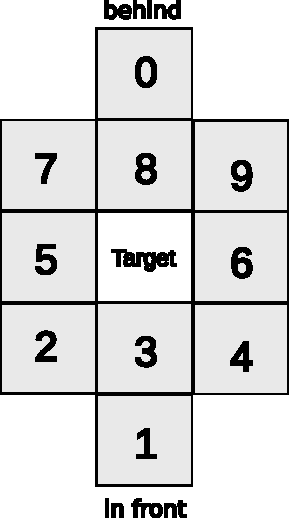
\includegraphics{index_files/mediabag/images/grenade-charg.pdf}

}

\caption{\label{fig-grenade}Grenade AOT}

\end{figure}%

\subsection{Oil}\label{oil}

A flask of oil can be used as a grenade-like missile. The oil must be
set afire in order to inflict damage; otherwise the oil is just
slippery. Assuming some means of igniting the oil is at hand, a direct
hit to a creature deals 1d8 points of fire damage, plus in the next
round the target takes an additional 1d8 points of damage, unless he or
she spends the round extinguishing the flames by some reasonable means.
The DM must judge the method used; rolling on the floor (assuming it's
not oily also) or covering the flames with a wet blanket are good
methods, for instance, while pouring or splashing water on burning oil
does little good. In any event, a flask of burning oil only causes
damage for two rounds at most.

If the oil is ignited by some sort of wick or fuse, then all other
creatures within 5 feet of the point of impact receive 1d6 points of
fire damage from the splash. A save vs.~Death Ray is allowed to avoid
this damage. If the flask does not hit the intended target (as described
under Grenade-Like Missiles, above), then that creature may still take
damage from the splash, and receives a saving throw. No saving throw is
allowed for a creature which has received a direct hit.

A flask of oil spilled or splattered on the ground will burn for 10
rounds. Those attempting to cross the burning oil will receive 1d6
points of fire damage each round they are in it (with no saving throw in
this case).

Fire-resistant creatures, including creatures having fire-based
abilities, are not damaged by burning oil.

\subsection{Holy Water}\label{holy-water}

Holy water damages undead creatures. A flask of holy water can be thrown
as a grenade-like missile; the flask breaks if thrown against the body
of a corporeal creature, but to use it against an incorporeal creature,
it must be opened and poured out onto the target, generally requiring
the attacker to be adjacent to the target.

A direct hit by a flask of holy water deals 1d8 points of damage to an
undead creature. In addition, each such creature within 5 feet of the
point of impact receives 1d6 points of damage from the splash. Holy
water is only effective for one round.

\subsection{Missiles That Miss}\label{missiles-that-miss}

With the exception of grenade-like missiles, missile weapons which miss
the intended target are normally considered lost. However, if the weapon
is fired into a melee where allies of the shooter are involved, and the
attack misses, it may hit one of the allied creatures. The DM should
decide which allies may be hit, and roll attacks against each until a
hit is made or all possible targets are exhausted. These attack rolls
are made with the shooter's normal attack bonus, just as if he or she
intended to attack the allied creature. However, the DM must make these
rolls, not the player.

This rule is applied to attacks made by monsters, when appropriate.
However, the DM still makes the rolls.

This rule is intentionally vague; the DM must decide when and how to
apply it based on the circumstances of the battle. It is recommended
that no more than three allies be ``tried'' in this way, but the DM may
make an exception as he or she sees fit.


\includegraphics{images/grappling.jpg}

\section{Grappling / Wrestling}\label{grappling-wrestling}

A grappling attack requires a Touch Attack (melee attack roll + attack
bonus, + either Str or Dex) Success indicates the attacker has grabbed
their opponent. A successful touch attack causes the attacker to move
into the same ``space'' as the defender. Both Sides make a Grapple Check
(D20+ attack bonus, + either Str or Dex, + Size Modifier) to determine
if this hold is maintained. Highest DC wins.

\begin{longtable}[]{@{}ll@{}}
\toprule\noalign{}
Size & Modifier \\
\midrule\noalign{}
\endhead
\bottomrule\noalign{}
\endlastfoot
Small & -4 \\
Medium & +0 \\
Large & +4 \\
\end{longtable}

After achieving a hold on an opponent, the attacker can automatically
inflict unarmed damage (as if striking with a fist), prevent a held
opponent from speaking, use simple magic items such as rings, or take
any other action the DM allows. The attacker may also attempt to acquire
an item the opponent is holding (such as a weapon) or attempt to move
the opponent (as described below). A held character may be voluntarily
released whenever the attacker so desires. The attacker can't draw or
use a weapon or use a wand, staff, scroll or potion, escape another's
wrestling attack, cast a spell, or pin another character while holding
an opponent.

\textbf{Moving the Opponent:}~The attacker can move up to one-half speed
(bringing the defender along) with a successful attack roll, if the
attacker is strong enough to carry or drag the defender.

\textbf{Acquiring an Object:}~The attacker may attempt to take an item
away from the defender. This requires an additional attack roll; if the
roll fails, the defender may immediately attempt an attack roll (even if
he or she has already attacked this round) which, if successful, results
in the defender pinning the attacker; or, the defender may choose to
escape instead of reversing the hold.

\textbf{Actions Allowed to the Defender:}~The target of a successful
hold is usually immobile (but not helpless) at least until his or her
next action, as determined by Initiative. Such characters suffer a
penalty of -4 to AC against opponents other than the attacker.

If the defender is significantly stronger and/or larger than the
attacker, he or she may move at up to one-half speed, dragging the
attacker along.

On the defender's next action, he or she can try to escape the pin with
a saving throw vs.~Death Ray; the defender must apply the better of his
or her Strength or Dexterity bonuses (or penalties) on this roll. If the
escape roll succeeds, the defender finishes the action by moving into
any space adjacent to the attacker.

If more than one attacker has a hold on a particular defender, a
successful escape roll frees the defender from just one of those
attackers.

Held characters may also use simple magic items such as rings. A
character being held may not normally cast a spell, even if he or she
has not been silenced by the attacker.

\textbf{Multiple Opponents:}~Several combatants can be involved in a
wrestling match. Up to four combatants can wrestle a single opponent of
normal size in a given round. Creatures that are smaller than the
attacker count for half, while creatures that are larger count at least
double (as determined by the DM). Note that, after an opponent is
pinned, other attackers benefit from the -4 AC penalty applied to the
defender. However, this AC penalty is not cumulative (that is, each
successful attack does not lower the defender's AC further).

It is also possible for another character to attack the attacker in an
ongoing wrestling bout. In this case, a successful hold on the attacker
grants the original defender a +4 bonus on subsequent escape rolls.

\textbf{Wrestling With Monsters:}~In general, the rules above can be
used not only when character races wrestle but also when humanoid
monsters are involved. The DM will decide whether or not to allow
wrestling involving non-humanoid creatures on a case-by-case basis; if
this is allowed, the following adjustments apply:

Creatures with extra grasping appendages (more than the usual two) gain
a +1 bonus on attack rolls or saving throws for each such appendage.
This includes creatures with feet capable of grasping (such as monkeys
or apes, giant spiders, etc.)

Large creatures able to fly may attempt to carry off their opponents
(even if the flying creature is the defender).

Wrestling attacks against creatures with touch attacks (such as wights)
will cause the attacker to suffer one such attack automatically every
round.

\section{Jousting}\label{jousting}

Jousting is a medieval sport where two combatants, mounted on horses,
charge at each other with lances, aiming to unhorse their opponent. It
is a display of skill, strength, and horsemanship, often held in
tournaments. The event is not only a test of combat prowess but also a
spectacle enjoyed by audiences, with knights in shining armor and
spirited horses adding to the grandeur.

\subsection{Rules}\label{rules}

\begin{itemize}
\item
  Only combatants are allowed on the field.
\item
  Only one attack is allowed for each mounted pass. Make a normal
  initiative roll to hit first.
\item
  Attackers ride applying a Charge against each other. (+2 for double
  damage), however, since all attacks are being done simultaneously, the
  AC penalty does not apply except for any other attacks that may be
  applied to either side by third parties.
\item
  When a jouster is hit by the other jouster, he must make a save versus
  Death Ray (however, CON does not modify this save, but add any Riding
  Skill bonus) or be unhorsed and land prone upon the ground.
\item
  If the save is failed by 4 or more, then the unhorsed individual is
  also stunned for 2 rounds (-2 penalty to AC as well as loss of DEX
  bonus if applicable and -2 penalty to attacks).
\item
  Each 5 points of damage dealt gives a -1 penalty to the save.
\item
  If the save is failed by 8 or more, the individual is Knocked Out
  completely.
\item
  A mounted opponent has a +2 chance to hit a mounted opponent's horse
  with sword, mace, flail, or another small weapon.
\item
  On a roll of a natural 1 to hit, a combatant's lance breaks on impact.
  The fighter may get another lance if his seconds provide them at their
  end of the bridge.
\item
  A mounted combatant using a sword, mace, flail, or other small weapon
  can't hit a mounted combatant using a lance.
\item
  Combat continues, mounted or on foot, until a clear winner emerges.
\item
  Jousts may be done using subdual damage instead of lethal damage
  (which is often the case in tournaments), generally by using blunted
  lances.
\end{itemize}

\section{Turning the Undead}\label{turning-the-undead-1}

Clerics can Turn undead, that is, drive away undead monsters by means of
faith alone. The Cleric brandishes their holy symbol and calls upon the
power of their divine patron. The player rolls 1d20 and adds their
Wisdom Bonus.

If the table indicates ``No'', it is not possible for the Cleric to
affect that type of undead monster. If the table gives a number, that is
the minimum number needed on 1d20 to Turn. Areas indicating ``T''
indicate that this type of undead is automatically affected. If the
result shown is a ``D,'' then the undead is destroyed rather than merely
Turned.

If the roll is a success, 2d6 + Wis hit dice of undead monsters are
affected. Surplus hit dice are lost (so if zombies are being Turned and
a roll of 7 is made, at most 3 zombies can be Turned), but a minimum of
one creature will always be affected if the first roll succeeds.

If a mixed group of undead is to be Turned, the result is checked
against the weakest first.

If a Cleric succeeds at Turning the undead, but not all undead monsters
present are affected, they may try again in the next round to turn any
remaining undead. If any roll to Turn the Undead fails, that Cleric may
not attempt to Turn Undead again for one full turn. A partial failure
(possible against a mixed group) counts as a failure for this purpose.
Turned Undead monsters flee from the Cleric at maximum movement. If the
party pursue and corner the Turned undead, they may resume attacking the
party; but if left alone, the monsters will not return or attempt to
attack the Cleric or those near them for at least 2d4 turns.

Undead monsters subject to a D (Damaged) result suffer 1d8 damage per
level of the Cleric (roll once and apply the same damage to all undead
monsters affected); those reduced to zero hit points are utterly
destroyed, being blasted into little fiery embers and ash. Those
surviving this damage are still Turned as above.

Note: Evil clerics can choose to command Undead rather than turn them.

\begin{figure*}

\begin{longtable}[]{@{}
  >{\raggedright\arraybackslash}p{(\columnwidth - 18\tabcolsep) * \real{0.1628}}
  >{\raggedright\arraybackslash}p{(\columnwidth - 18\tabcolsep) * \real{0.1163}}
  >{\raggedright\arraybackslash}p{(\columnwidth - 18\tabcolsep) * \real{0.0930}}
  >{\raggedright\arraybackslash}p{(\columnwidth - 18\tabcolsep) * \real{0.0814}}
  >{\raggedright\arraybackslash}p{(\columnwidth - 18\tabcolsep) * \real{0.0814}}
  >{\raggedright\arraybackslash}p{(\columnwidth - 18\tabcolsep) * \real{0.0930}}
  >{\raggedright\arraybackslash}p{(\columnwidth - 18\tabcolsep) * \real{0.0814}}
  >{\raggedright\arraybackslash}p{(\columnwidth - 18\tabcolsep) * \real{0.1047}}
  >{\raggedright\arraybackslash}p{(\columnwidth - 18\tabcolsep) * \real{0.1047}}
  >{\raggedright\arraybackslash}p{(\columnwidth - 18\tabcolsep) * \real{0.0814}}@{}}
\toprule\noalign{}
\begin{minipage}[b]{\linewidth}\raggedright
Cleric Lvl
\end{minipage} & \begin{minipage}[b]{\linewidth}\raggedright
Skeleton
\end{minipage} & \begin{minipage}[b]{\linewidth}\raggedright
Zombie
\end{minipage} & \begin{minipage}[b]{\linewidth}\raggedright
Ghoul
\end{minipage} & \begin{minipage}[b]{\linewidth}\raggedright
Wight
\end{minipage} & \begin{minipage}[b]{\linewidth}\raggedright
Wraith
\end{minipage} & \begin{minipage}[b]{\linewidth}\raggedright
Mummy
\end{minipage} & \begin{minipage}[b]{\linewidth}\raggedright
Spectre
\end{minipage} & \begin{minipage}[b]{\linewidth}\raggedright
Vampire
\end{minipage} & \begin{minipage}[b]{\linewidth}\raggedright
Ghost
\end{minipage} \\
\midrule\noalign{}
\endhead
\bottomrule\noalign{}
\endlastfoot
& 1 HD & 2 HD & 3 HD & 4 HD & 5 HD & 6 HD & 7 HD & 8 HD & 9+ HD \\
1 & 13 & 17 & 19 & No & No & No & No & No & No \\
2 & 11 & 15 & 18 & 20 & No & No & No & No & No \\
3 & 9 & 13 & 17 & 19 & No & No & No & No & No \\
4 & 7 & 11 & 15 & 18 & 20 & No & No & No & No \\
5 & 5 & 9 & 13 & 17 & 19 & No & No & No & No \\
6 & 3 & 7 & 11 & 15 & 18 & 20 & No & No & No \\
7 & 2 & 5 & 9 & 13 & 17 & 19 & No & No & No \\
8 & T & 3 & 7 & 11 & 15 & 18 & 20 & No & No \\
9 & T & 2 & 5 & 9 & 13 & 17 & 19 & No & No \\
10 & T & T & 3 & 7 & 11 & 15 & 18 & 20 & No \\
11 & D & T & 2 & 5 & 9 & 13 & 17 & 19 & No \\
12 & D & T & T & 3 & 7 & 11 & 15 & 18 & 20 \\
13 & D & D & T & 2 & 5 & 9 & 13 & 17 & 19 \\
14 & D & D & T & T & 3 & 7 & 11 & 15 & 18 \\
15 & D & D & D & T & 2 & 5 & 9 & 13 & 17 \\
16 & D & D & D & T & T & 3 & 7 & 11 & 15 \\
17 & D & D & D & D & T & 2 & 5 & 9 & 13 \\
18 & D & D & D & D & T & T & 3 & 7 & 11 \\
19 & D & D & D & D & D & T & 2 & 5 & 9 \\
20 & D & D & D & D & D & T & T & 3 & 7 \\
\end{longtable}

\end{figure*}%

\begin{Shaded}
\begin{Highlighting}[]
\NormalTok{viewof level = Inputs.select([1,2,3,4,5,6,7,8,9,10,11,12,13,14,15,16,17,18,19,20], \{value:1, label: "Cleric Level"\})}

\NormalTok{viewof r = Inputs.select([1,2,3,4,5,6,7,8,9,10,11,12,13,14,15,16,17,18,19,20], \{value:1, label: "Roll"\})}
\end{Highlighting}
\end{Shaded}

\begin{Shaded}
\begin{Highlighting}[]
\NormalTok{import \{turnUndead\} from "./custom.js"}

\NormalTok{res = turnUndead(level,r)}
\end{Highlighting}
\end{Shaded}

\$\{res\}

\section{Attacking a Vehicle}\label{attacking-a-vehicle}

Attacks against vehicles (such as wagons or ships) are made against
Armor Class 11. Each vehicle has listed Hardness and Hit Point values.
Roll damage against the vehicle, and then reduce that damage by the
Hardness value. Any excess damage is applied to the vehicle.

If the vehicle takes damage equal to or greater than the listed HP on
one side, it is reduced to half speed due to wheel damage or a hull
breach; if it takes this much again, it is immobilized, and this much
damage will sink a ship.

\subsection{Repairing a Vehicle}\label{repairing-a-vehicle}

Damage done to a vehicle may be restored at a rate of 1d4 hit points per
crew member per hour of labor. However, a vehicle can only be restored
to 90\% of its maximum hit points by field repairs; a damaged ship must
be put into drydock and repaired by a shipwright and his crew, while a
wagon, cart or chariot will require a wagonmaker to repair them. Costs
of such repairs are left to the Dungeon Master to decide.

\chapter{Saving Throws}\label{saving-throws}

\textbf{Saving throws}~represent the ability of a character or creature
to resist or avoid special attacks, such as spells or poisons. Like an
attack roll, a saving throw is a d20 roll, with a target number based on
the character's class and level; for monsters, a comparable class and
level are provided for the purpose of determining the monster's saving
throw figures. A natural (unadjusted) roll of 1 on a saving throw is
always a failure, while a natural 20 is always a success.

The five categories of saving throw as follows:~\textbf{Death Ray or
Poison},~\textbf{Magic Wands},~\textbf{Paralysis or
Petrify},~\textbf{Dragon Breath}, and~\textbf{Spells}. Spells and
monster special attacks will indicate which category applies (when a
saving throw is allowed), but in some unusual situations the Dungeon
Master will need to choose a category. One way to make this choice is to
interpret the categories metaphorically. For example, a DM might be
writing an adventure wherein there is a trap that pours burning oil on
the hapless adventurers. Avoiding the oil might be considered similar to
avoiding Dragon Breath. Or perhaps a stone idol shoots beams of energy
from its glaring eyes when approached. This attack may be considered
similar to a Magic Wand, or if especially potent, a Spell. Another
approach is to interpret the categories in terms of which ability is
challenged:

\begin{itemize}
\tightlist
\item
  Death Ray or Poison (Constitution)
\item
  Magic Wands (Wisdom)
\item
  Paralysis or Petrify (Strength)
\item
  Dragon Breath (Dexterity)
\item
  Spells (Intelligence).~
\end{itemize}

The saving throw vs.~Death Ray is often used as a ``catch all'' save
versus many of the ``ordinary'' dangers encountered in a dungeon
environment.

In general, saving throw rolls are not adjusted by ability score bonus
or penalty figures. There are a few exceptions:

\begin{itemize}
\tightlist
\item
  Poison saving throws are always adjusted by the character's
  \hyperref[ability-scores]{Constitution} modifier.
\item
  Saving throws against illusions (such as~\textbf{phantasmal force})
  are always adjusted by the character's
  \hyperref[ability-scores]{Intelligence} modifier.
\item
  Saving throws against~\textbf{charm}~spells (and other forms of mind
  control) are adjusted by the character's
  \hyperref[ability-scores]{Wisdom} modifier.
\end{itemize}

The DM may decide on other saving throw adjustments as he or she sees
fit.

\section{Item Saving Throws}\label{item-saving-throws}

Area effects (such as fireball or lightning bolt spells) may damage
items carried by a character as well as injuring the character. For
simplicity, assume that items carried are unaffected if the character or
creature carrying them makes his or her own saving throw. However, very
fragile items (paper vs.~fire, glass vs.~physical impact, etc.) may
still be considered subject to damage even if the bearer makes his or
her save.

In any case where one or more items may be subject to damage, use the
saving throw roll of the bearer to determine if the item is damaged or
not. For example, a character holding an open spellbook is struck by a
fireball spell; he or she must save vs.~Spells, and then save again at
the same odds for the spellbook.

The DM should feel free to amend this rule as he or she wishes; for
instance, a backpack full of fragile items might be given a single
saving throw rather than laboriously rolling for each and every item.

\section{Saving Throw Tables by
Class}\label{saving-throw-tables-by-class}

\begin{longtable}[]{@{}
  >{\raggedright\arraybackslash}p{(\columnwidth - 10\tabcolsep) * \real{0.1264}}
  >{\raggedright\arraybackslash}p{(\columnwidth - 10\tabcolsep) * \real{0.2299}}
  >{\raggedright\arraybackslash}p{(\columnwidth - 10\tabcolsep) * \real{0.1494}}
  >{\raggedright\arraybackslash}p{(\columnwidth - 10\tabcolsep) * \real{0.2414}}
  >{\raggedright\arraybackslash}p{(\columnwidth - 10\tabcolsep) * \real{0.1724}}
  >{\raggedright\arraybackslash}p{(\columnwidth - 10\tabcolsep) * \real{0.0805}}@{}}
\caption{Cleric Saving Throws}\label{tbl-save-clerics-2}\tabularnewline
\toprule\noalign{}
\begin{minipage}[b]{\linewidth}\raggedright
\textbf{Level}
\end{minipage} & \begin{minipage}[b]{\linewidth}\raggedright
Death Ray / Poison
\end{minipage} & \begin{minipage}[b]{\linewidth}\raggedright
Magic Wands
\end{minipage} & \begin{minipage}[b]{\linewidth}\raggedright
Paralysis / Petrify
\end{minipage} & \begin{minipage}[b]{\linewidth}\raggedright
Dragon Breath
\end{minipage} & \begin{minipage}[b]{\linewidth}\raggedright
Spells
\end{minipage} \\
\midrule\noalign{}
\endfirsthead
\toprule\noalign{}
\begin{minipage}[b]{\linewidth}\raggedright
\textbf{Level}
\end{minipage} & \begin{minipage}[b]{\linewidth}\raggedright
Death Ray / Poison
\end{minipage} & \begin{minipage}[b]{\linewidth}\raggedright
Magic Wands
\end{minipage} & \begin{minipage}[b]{\linewidth}\raggedright
Paralysis / Petrify
\end{minipage} & \begin{minipage}[b]{\linewidth}\raggedright
Dragon Breath
\end{minipage} & \begin{minipage}[b]{\linewidth}\raggedright
Spells
\end{minipage} \\
\midrule\noalign{}
\endhead
\bottomrule\noalign{}
\endlastfoot
\textbf{1} & 11 & 12 & 14 & 16 & 15 \\
\textbf{2-3} & 10 & 11 & 13 & 15 & 14 \\
\textbf{4-5} & 9 & 10 & 13 & 15 & 14 \\
\textbf{6-7} & 9 & 10 & 12 & 14 & 13 \\
\textbf{8-9} & 8 & 9 & 12 & 14 & 13 \\
\textbf{10-11} & 8 & 9 & 11 & 13 & 12 \\
\textbf{12-13} & 7 & 8 & 11 & 13 & 12 \\
\textbf{14-15} & 7 & 8 & 10 & 12 & 11 \\
\textbf{16-17} & 6 & 7 & 10 & 12 & 11 \\
\textbf{18-19} & 6 & 7 & 9 & 11 & 10 \\
\textbf{20} & 5 & 6 & 9 & 11 & 10 \\
\end{longtable}

\begin{longtable}[]{@{}
  >{\raggedright\arraybackslash}p{(\columnwidth - 10\tabcolsep) * \real{0.1250}}
  >{\raggedright\arraybackslash}p{(\columnwidth - 10\tabcolsep) * \real{0.2273}}
  >{\raggedright\arraybackslash}p{(\columnwidth - 10\tabcolsep) * \real{0.1477}}
  >{\raggedright\arraybackslash}p{(\columnwidth - 10\tabcolsep) * \real{0.2386}}
  >{\raggedright\arraybackslash}p{(\columnwidth - 10\tabcolsep) * \real{0.1705}}
  >{\raggedright\arraybackslash}p{(\columnwidth - 10\tabcolsep) * \real{0.0909}}@{}}
\caption{Druid Saving Throws}\label{tbl-save-druids-2}\tabularnewline
\toprule\noalign{}
\begin{minipage}[b]{\linewidth}\raggedright
\textbf{Level}
\end{minipage} & \begin{minipage}[b]{\linewidth}\raggedright
Death Ray / Poison
\end{minipage} & \begin{minipage}[b]{\linewidth}\raggedright
Magic Wands
\end{minipage} & \begin{minipage}[b]{\linewidth}\raggedright
Paralysis / Petrify
\end{minipage} & \begin{minipage}[b]{\linewidth}\raggedright
Dragon Breath
\end{minipage} & \begin{minipage}[b]{\linewidth}\raggedright
Spells
\end{minipage} \\
\midrule\noalign{}
\endfirsthead
\toprule\noalign{}
\begin{minipage}[b]{\linewidth}\raggedright
\textbf{Level}
\end{minipage} & \begin{minipage}[b]{\linewidth}\raggedright
Death Ray / Poison
\end{minipage} & \begin{minipage}[b]{\linewidth}\raggedright
Magic Wands
\end{minipage} & \begin{minipage}[b]{\linewidth}\raggedright
Paralysis / Petrify
\end{minipage} & \begin{minipage}[b]{\linewidth}\raggedright
Dragon Breath
\end{minipage} & \begin{minipage}[b]{\linewidth}\raggedright
Spells
\end{minipage} \\
\midrule\noalign{}
\endhead
\bottomrule\noalign{}
\endlastfoot
\textbf{1} & 13 & 14 & 13 & 16 & 15 \\
\textbf{2-3} & 13 & 14 & 13 & 15 & 14 \\
\textbf{4-5} & 12 & 13 & 12 & 15 & 13 \\
\textbf{6-7} & 12 & 12 & 11 & 14 & 13 \\
\textbf{8-9} & 11 & 11 & 10 & 14 & 12 \\
\textbf{10-11} & 11 & 10 & 9 & 13 & 11 \\
\textbf{12-13} & 10 & 10 & 9 & 13 & 11 \\
\textbf{14-15} & 10 & 9 & 8 & 12 & 10 \\
\textbf{16-17} & 9 & 8 & 7 & 12 & 9 \\
\textbf{18-19} & 9 & 7 & 6 & 11 & 9 \\
\textbf{20} & 8 & 6 & 5 & 11 & 8 \\
\end{longtable}

\begin{longtable}[]{@{}
  >{\raggedright\arraybackslash}p{(\columnwidth - 10\tabcolsep) * \real{0.1264}}
  >{\raggedright\arraybackslash}p{(\columnwidth - 10\tabcolsep) * \real{0.2299}}
  >{\raggedright\arraybackslash}p{(\columnwidth - 10\tabcolsep) * \real{0.1494}}
  >{\raggedright\arraybackslash}p{(\columnwidth - 10\tabcolsep) * \real{0.2414}}
  >{\raggedright\arraybackslash}p{(\columnwidth - 10\tabcolsep) * \real{0.1724}}
  >{\raggedright\arraybackslash}p{(\columnwidth - 10\tabcolsep) * \real{0.0805}}@{}}
\caption{Fighter Saving Throws}\label{tbl-save-fighter-2}\tabularnewline
\toprule\noalign{}
\begin{minipage}[b]{\linewidth}\raggedright
\textbf{Level}
\end{minipage} & \begin{minipage}[b]{\linewidth}\raggedright
Death Ray / Poison
\end{minipage} & \begin{minipage}[b]{\linewidth}\raggedright
Magic Wands
\end{minipage} & \begin{minipage}[b]{\linewidth}\raggedright
Paralysis / Petrify
\end{minipage} & \begin{minipage}[b]{\linewidth}\raggedright
Dragon Breath
\end{minipage} & \begin{minipage}[b]{\linewidth}\raggedright
Spells
\end{minipage} \\
\midrule\noalign{}
\endfirsthead
\toprule\noalign{}
\begin{minipage}[b]{\linewidth}\raggedright
\textbf{Level}
\end{minipage} & \begin{minipage}[b]{\linewidth}\raggedright
Death Ray / Poison
\end{minipage} & \begin{minipage}[b]{\linewidth}\raggedright
Magic Wands
\end{minipage} & \begin{minipage}[b]{\linewidth}\raggedright
Paralysis / Petrify
\end{minipage} & \begin{minipage}[b]{\linewidth}\raggedright
Dragon Breath
\end{minipage} & \begin{minipage}[b]{\linewidth}\raggedright
Spells
\end{minipage} \\
\midrule\noalign{}
\endhead
\bottomrule\noalign{}
\endlastfoot
\textbf{NM} & 13 & 14 & 15 & 16 & 18 \\
\textbf{1} & 12 & 13 & 14 & 15 & 17 \\
\textbf{2-3} & 11 & 12 & 14 & 15 & 16 \\
\textbf{4-5} & 11 & 11 & 13 & 14 & 15 \\
\textbf{6-7} & 10 & 11 & 12 & 14 & 15 \\
\textbf{8-9} & 9 & 10 & 12 & 13 & 14 \\
\textbf{10-11} & 9 & 9 & 11 & 12 & 13 \\
\textbf{12-13} & 8 & 9 & 10 & 12 & 13 \\
\textbf{14-15} & 7 & 8 & 10 & 11 & 12 \\
\textbf{16-17} & 7 & 7 & 9 & 10 & 11 \\
\textbf{18-19} & 6 & 7 & 8 & 10 & 11 \\
\textbf{20} & 5 & 6 & 8 & 9 & 10 \\
\end{longtable}

\begin{longtable}[]{@{}
  >{\raggedright\arraybackslash}p{(\columnwidth - 10\tabcolsep) * \real{0.1250}}
  >{\raggedright\arraybackslash}p{(\columnwidth - 10\tabcolsep) * \real{0.2273}}
  >{\raggedright\arraybackslash}p{(\columnwidth - 10\tabcolsep) * \real{0.1477}}
  >{\raggedright\arraybackslash}p{(\columnwidth - 10\tabcolsep) * \real{0.2386}}
  >{\raggedright\arraybackslash}p{(\columnwidth - 10\tabcolsep) * \real{0.1705}}
  >{\raggedright\arraybackslash}p{(\columnwidth - 10\tabcolsep) * \real{0.0909}}@{}}
\caption{Paladin Saving Throws}\label{tbl-save-paladin-2}\tabularnewline
\toprule\noalign{}
\begin{minipage}[b]{\linewidth}\raggedright
\textbf{Level}
\end{minipage} & \begin{minipage}[b]{\linewidth}\raggedright
Death Ray / Poison
\end{minipage} & \begin{minipage}[b]{\linewidth}\raggedright
Magic Wands
\end{minipage} & \begin{minipage}[b]{\linewidth}\raggedright
Paralysis / Petrify
\end{minipage} & \begin{minipage}[b]{\linewidth}\raggedright
Dragon Breath
\end{minipage} & \begin{minipage}[b]{\linewidth}\raggedright
Spells
\end{minipage} \\
\midrule\noalign{}
\endfirsthead
\toprule\noalign{}
\begin{minipage}[b]{\linewidth}\raggedright
\textbf{Level}
\end{minipage} & \begin{minipage}[b]{\linewidth}\raggedright
Death Ray / Poison
\end{minipage} & \begin{minipage}[b]{\linewidth}\raggedright
Magic Wands
\end{minipage} & \begin{minipage}[b]{\linewidth}\raggedright
Paralysis / Petrify
\end{minipage} & \begin{minipage}[b]{\linewidth}\raggedright
Dragon Breath
\end{minipage} & \begin{minipage}[b]{\linewidth}\raggedright
Spells
\end{minipage} \\
\midrule\noalign{}
\endhead
\bottomrule\noalign{}
\endlastfoot
\textbf{NM} & 13 & 14 & 15 & 16 & 18 \\
\textbf{1} & 12 & 13 & 14 & 15 & 17 \\
\textbf{2-3} & 11 & 12 & 14 & 15 & 16 \\
\textbf{4-5} & 11 & 11 & 13 & 14 & 15 \\
\textbf{6-7} & 10 & 11 & 12 & 14 & 15 \\
\textbf{8-9} & 9 & 10 & 12 & 13 & 14 \\
\textbf{10-11} & 9 & 9 & 11 & 12 & 13 \\
\textbf{12-13} & 8 & 9 & 10 & 12 & 13 \\
\textbf{14-15} & 7 & 8 & 10 & 11 & 12 \\
\textbf{16-17} & 7 & 7 & 9 & 10 & 11 \\
\textbf{18-19} & 6 & 7 & 8 & 10 & 11 \\
\textbf{20} & 5 & 6 & 8 & 9 & 10 \\
\end{longtable}

\begin{longtable}[]{@{}
  >{\raggedright\arraybackslash}p{(\columnwidth - 10\tabcolsep) * \real{0.1250}}
  >{\raggedright\arraybackslash}p{(\columnwidth - 10\tabcolsep) * \real{0.2273}}
  >{\raggedright\arraybackslash}p{(\columnwidth - 10\tabcolsep) * \real{0.1477}}
  >{\raggedright\arraybackslash}p{(\columnwidth - 10\tabcolsep) * \real{0.2386}}
  >{\raggedright\arraybackslash}p{(\columnwidth - 10\tabcolsep) * \real{0.1705}}
  >{\raggedright\arraybackslash}p{(\columnwidth - 10\tabcolsep) * \real{0.0909}}@{}}
\caption{Ranger Saving Throws}\label{tbl-save-ranger-2}\tabularnewline
\toprule\noalign{}
\begin{minipage}[b]{\linewidth}\raggedright
\textbf{Level}
\end{minipage} & \begin{minipage}[b]{\linewidth}\raggedright
Death Ray / Poison
\end{minipage} & \begin{minipage}[b]{\linewidth}\raggedright
Magic Wands
\end{minipage} & \begin{minipage}[b]{\linewidth}\raggedright
Paralysis / Petrify
\end{minipage} & \begin{minipage}[b]{\linewidth}\raggedright
Dragon Breath
\end{minipage} & \begin{minipage}[b]{\linewidth}\raggedright
Spells
\end{minipage} \\
\midrule\noalign{}
\endfirsthead
\toprule\noalign{}
\begin{minipage}[b]{\linewidth}\raggedright
\textbf{Level}
\end{minipage} & \begin{minipage}[b]{\linewidth}\raggedright
Death Ray / Poison
\end{minipage} & \begin{minipage}[b]{\linewidth}\raggedright
Magic Wands
\end{minipage} & \begin{minipage}[b]{\linewidth}\raggedright
Paralysis / Petrify
\end{minipage} & \begin{minipage}[b]{\linewidth}\raggedright
Dragon Breath
\end{minipage} & \begin{minipage}[b]{\linewidth}\raggedright
Spells
\end{minipage} \\
\midrule\noalign{}
\endhead
\bottomrule\noalign{}
\endlastfoot
1 & 12 & 13 & 14 & 15 & 17 \\
2-3 & 11 & 12 & 14 & 15 & 16 \\
4-5 & 11 & 11 & 13 & 14 & 15 \\
6-7 & 10 & 11 & 12 & 14 & 15 \\
8-9 & 9 & 10 & 12 & 13 & 14 \\
10-11 & 9 & 9 & 11 & 12 & 13 \\
12-13 & 8 & 9 & 10 & 12 & 13 \\
14-15 & 7 & 8 & 10 & 11 & 12 \\
16-17 & 7 & 7 & 9 & 10 & 11 \\
18-19 & 6 & 7 & 8 & 10 & 11 \\
20 & 5 & 6 & 8 & 9 & 10 \\
\end{longtable}

\begin{longtable}[]{@{}
  >{\raggedright\arraybackslash}p{(\columnwidth - 10\tabcolsep) * \real{0.1264}}
  >{\raggedright\arraybackslash}p{(\columnwidth - 10\tabcolsep) * \real{0.2299}}
  >{\raggedright\arraybackslash}p{(\columnwidth - 10\tabcolsep) * \real{0.1494}}
  >{\raggedright\arraybackslash}p{(\columnwidth - 10\tabcolsep) * \real{0.2414}}
  >{\raggedright\arraybackslash}p{(\columnwidth - 10\tabcolsep) * \real{0.1724}}
  >{\raggedright\arraybackslash}p{(\columnwidth - 10\tabcolsep) * \real{0.0805}}@{}}
\caption{Magic-User Saving Throws}\label{tbl-save-mage-2}\tabularnewline
\toprule\noalign{}
\begin{minipage}[b]{\linewidth}\raggedright
\textbf{Level}
\end{minipage} & \begin{minipage}[b]{\linewidth}\raggedright
Death Ray / Poison
\end{minipage} & \begin{minipage}[b]{\linewidth}\raggedright
Magic Wands
\end{minipage} & \begin{minipage}[b]{\linewidth}\raggedright
Paralysis / Petrify
\end{minipage} & \begin{minipage}[b]{\linewidth}\raggedright
Dragon Breath
\end{minipage} & \begin{minipage}[b]{\linewidth}\raggedright
Spells
\end{minipage} \\
\midrule\noalign{}
\endfirsthead
\toprule\noalign{}
\begin{minipage}[b]{\linewidth}\raggedright
\textbf{Level}
\end{minipage} & \begin{minipage}[b]{\linewidth}\raggedright
Death Ray / Poison
\end{minipage} & \begin{minipage}[b]{\linewidth}\raggedright
Magic Wands
\end{minipage} & \begin{minipage}[b]{\linewidth}\raggedright
Paralysis / Petrify
\end{minipage} & \begin{minipage}[b]{\linewidth}\raggedright
Dragon Breath
\end{minipage} & \begin{minipage}[b]{\linewidth}\raggedright
Spells
\end{minipage} \\
\midrule\noalign{}
\endhead
\bottomrule\noalign{}
\endlastfoot
\textbf{1} & 13 & 14 & 13 & 16 & 15 \\
\textbf{2-3} & 13 & 14 & 13 & 15 & 14 \\
\textbf{4-5} & 12 & 13 & 12 & 15 & 13 \\
\textbf{6-7} & 12 & 12 & 11 & 14 & 13 \\
\textbf{8-9} & 11 & 11 & 10 & 14 & 12 \\
\textbf{10-11} & 11 & 10 & 9 & 13 & 11 \\
\textbf{12-13} & 10 & 10 & 9 & 13 & 11 \\
\textbf{14-15} & 10 & 9 & 8 & 12 & 10 \\
\textbf{16-17} & 9 & 8 & 7 & 12 & 9 \\
\textbf{18-19} & 9 & 7 & 6 & 11 & 9 \\
\textbf{20} & 8 & 6 & 5 & 11 & 8 \\
\end{longtable}

\begin{longtable}[]{@{}
  >{\raggedright\arraybackslash}p{(\columnwidth - 10\tabcolsep) * \real{0.1264}}
  >{\raggedright\arraybackslash}p{(\columnwidth - 10\tabcolsep) * \real{0.2299}}
  >{\raggedright\arraybackslash}p{(\columnwidth - 10\tabcolsep) * \real{0.1494}}
  >{\raggedright\arraybackslash}p{(\columnwidth - 10\tabcolsep) * \real{0.2414}}
  >{\raggedright\arraybackslash}p{(\columnwidth - 10\tabcolsep) * \real{0.1724}}
  >{\raggedright\arraybackslash}p{(\columnwidth - 10\tabcolsep) * \real{0.0805}}@{}}
\caption{Thief Saving Throws}\label{tbl-save-thief-2}\tabularnewline
\toprule\noalign{}
\begin{minipage}[b]{\linewidth}\raggedright
\textbf{Level}
\end{minipage} & \begin{minipage}[b]{\linewidth}\raggedright
Death Ray / Poison
\end{minipage} & \begin{minipage}[b]{\linewidth}\raggedright
Magic Wands
\end{minipage} & \begin{minipage}[b]{\linewidth}\raggedright
Paralysis / Petrify
\end{minipage} & \begin{minipage}[b]{\linewidth}\raggedright
Dragon Breath
\end{minipage} & \begin{minipage}[b]{\linewidth}\raggedright
Spells
\end{minipage} \\
\midrule\noalign{}
\endfirsthead
\toprule\noalign{}
\begin{minipage}[b]{\linewidth}\raggedright
\textbf{Level}
\end{minipage} & \begin{minipage}[b]{\linewidth}\raggedright
Death Ray / Poison
\end{minipage} & \begin{minipage}[b]{\linewidth}\raggedright
Magic Wands
\end{minipage} & \begin{minipage}[b]{\linewidth}\raggedright
Paralysis / Petrify
\end{minipage} & \begin{minipage}[b]{\linewidth}\raggedright
Dragon Breath
\end{minipage} & \begin{minipage}[b]{\linewidth}\raggedright
Spells
\end{minipage} \\
\midrule\noalign{}
\endhead
\bottomrule\noalign{}
\endlastfoot
\textbf{1} & 13 & 14 & 13 & 16 & 15 \\
\textbf{2-3} & 12 & 14 & 12 & 15 & 14 \\
\textbf{4-5} & 11 & 13 & 12 & 14 & 13 \\
\textbf{6-7} & 11 & 13 & 11 & 13 & 13 \\
\textbf{8-9} & 10 & 12 & 11 & 12 & 12 \\
\textbf{10-11} & 9 & 12 & 10 & 11 & 11 \\
\textbf{12-13} & 9 & 10 & 10 & 10 & 11 \\
\textbf{14-15} & 8 & 10 & 9 & 9 & 10 \\
\textbf{16-17} & 7 & 9 & 9 & 8 & 9 \\
\textbf{18-19} & 7 & 9 & 8 & 7 & 9 \\
\textbf{20} & 6 & 8 & 8 & 6 & 8 \\
\end{longtable}

\section{Difficulty Challenge (DC)}\label{difficulty-challenge-dc}

There will be times when a player character tries to do something in the
game that seems to have no rule covering it. In some of those cases, the
DM will assign a Difficulty Challenge (DC) number from 1 to 20. The
player rolls 1d20 and adds their Ability Bonus for the score the DM
thinks is most appropriate, as well as any situational bonus or penalty
the DM assigns. The resulting number must equal or be greater than the
DC number.

\begin{longtable}[]{@{}llll@{}}
\caption{Difficulty
Challenge}\label{tbl-difficulty-challege}\tabularnewline
\toprule\noalign{}
Percentile\% (2d10) & (1d6) & (1d20) & Description \\
\midrule\noalign{}
\endfirsthead
\toprule\noalign{}
Percentile\% (2d10) & (1d6) & (1d20) & Description \\
\midrule\noalign{}
\endhead
\bottomrule\noalign{}
\endlastfoot
85\% & 1-5 & DC 3 & Very Easy \\
70\% & 1-4 & DC 6 & Easy \\
50\% & 1-3 & DC 10 & Normal \\
35\% & 1-2 & DC 13 & Hard \\
15\% & 1-1 & DC 15 & Very Hard \\
5\% & - & DC 20 & Extremely Difficult \\
\end{longtable}

\chapter{Healing and Injuries}\label{healing-and-injuries}

\section{Healing and Rest}\label{healing-and-rest-1}

Characters recover 1 hit point of damage every day, provided that normal
sleep is possible. Characters who choose full bedrest regain an
additional hit point each evening.

Normal characters require 6 hours sleep out of every 24. Subtract from
this number of hours the character's Constitution bonus; so a character
with 18 Constitution needs only 3 hours sleep per night (and a character
with 3 Constitution needs 9 hours). Note that these figures are
minimums; given a choice, most characters would prefer to sleep two or
more hours longer.

Characters who get less than the required amount of sleep suffer a
\textbf{-1 penalty} on all attack rolls and saving throws (as well as
not receiving any hit points of healing). For each additional night
where sufficient sleep is not received, the penalty becomes one point
worse. Regardless of how long the character has gone without adequate
sleep, the normal amount of sleep will remove these penalties.

\section{Conditional States}\label{conditional-states}

If more than one condition affects a character, apply them all. If
certain effects can't combine, apply the most severe effect.

\subsection{Ability Damaged and Constitution Point
Losses}\label{ability-damaged-and-constitution-point-losses}

When a creature suffers ability damage, it temporarily loses 1 or more
points from one or more ability scores. Lost points return at a rate of
1 per day unless otherwise noted by the condition causing the damage.

\begin{itemize}
\tightlist
\item
  A creature with Strength 0 falls to the ground and is helpless.
\item
  A creature with Dexterity 0 is paralyzed.
\item
  A creature with Constitution 0 is dead.
\item
  A creature with Intelligence, Wisdom, or Charisma 0 is unconscious.
\end{itemize}

Ability damage differs from penalties to ability scores, which disappear
once the conditions causing them go away.

\subsubsection{Constitution Point
Losses}\label{constitution-point-losses}

When a character temporarily loses Constitution points (such as due to a
disease), they may regain them with normal rest. The recovery rate is
one point per day, awarded each morning after a normal night's sleep. If
more than one Constitution point was lost, the character must make a
save vs.~Death Ray (without adjustments) to regain the final point;
failure results in the permanent loss of that point.

If a temporary Constitution loss results in a lower bonus or penalty,
the character's maximum hit points must be adjusted accordingly. For
example, if a character's Constitution drops from 16 to 15, their bonus
decreases from +2 to +1, resulting in a loss of one hit point per die
rolled. If this adjustment reduces the maximum hit points to less than
the current hit points, the current hit points are immediately reduced
to the new maximum.

When regaining Constitution, any increase that raises the character's
Constitution bonus restores the lost hit points to the maximum hit point
figure only. Current hit points must be regained through normal healing
methods.

\subsection{Blindness}\label{blindness}

A blinded creature suffers the following effects:

\begin{itemize}
\tightlist
\item
  A -4 penalty to attack rolls.
\item
  A -4 penalty to Armor Class.
\item
  A -2 penalty to Initiative rolls.
\item
  Movement is at half speed.
\item
  The creature is surprised on a DC 6 check.
\end{itemize}

These effects may be modified for creatures with unusual sensory
abilities. For example, bats may be affected by deafness as if blinded
instead. These penalties apply primarily to characters or creatures
recently handicapped. Those who are normally blind may have reduced
penalties at the DM's discretion.

\subsection{Blown Away}\label{blown-away}

Depending on its size, a creature can be blown away by winds of high
velocity.

\begin{itemize}
\item
  A creature on the ground that is blown away is knocked down and rolls
  1d4 × 10 feet, taking 1d4 points of nonlethal damage per 10 feet.
\item
  A flying creature that is blown away is pushed back 2d6 × 10 feet and
  takes 2d6 points of nonlethal damage due to battering and buffeting.
\end{itemize}

\subsection{Checked}\label{checked}

Prevented from achieving forward motion by an applied force, such as
wind. Checked creatures on the ground merely stop. Checked flying
creatures move back a distance specified in the description of the
effect.

\subsection{Confused}\label{confused}

A confused creature's actions are determined by rolling a d20 at the
beginning of its turn:

\begin{itemize}
\tightlist
\item
  1-3: Attack caster with melee or ranged weapons (or close with caster
  if attacking is not possible).
\item
  4-8: Act normally.
\item
  9-13: Do nothing but babble incoherently.
\item
  14-17: Flee away from caster at top possible speed.
\item
  18-20: Attack nearest creature (for this purpose, a familiar counts as
  part of the subject's self).
\end{itemize}

A confused creature that can't carry out the indicated action does
nothing but babble incoherently. Attackers are not at any special
advantage when attacking a confused character. Any confused character
that is attacked automatically attacks its attackers on its next turn if
it is still confused.

A confused creature does not make attacks of opportunity against any
creature that it is not already devoted to attacking (either because of
its most recent action or because it has just been attacked).

\subsection{Cowering}\label{cowering}

The creature is frozen in fear and can take no actions. A cowering
creature takes a -2 penalty to Armor Class and loses its Dexterity
bonus.

\subsection{Dazed}\label{dazed}

The creature is unable to act normally. A dazed creature can take no
actions but has no penalty to AC. A dazed condition typically lasts 1
round.

\subsection{Dazzled}\label{dazzled}

The creature is unable to see well because of overstimulation of the
eyes. A dazzled creature takes a -1 penalty on attack rolls, Search
checks, and Spot checks.

\subsection{Dead}\label{dead}

The creature's hit points are reduced to -10, its Constitution drops to
0, or it is killed outright by a spell or effect. The character's soul
leaves its body. Dead creatures cannot benefit from normal or magical
healing, but they can be restored to life via magic.

A dead body decays normally unless magically preserved, but magic that
restores a dead character to life also restores the body either to full
health or to its condition at the time of death (depending on the spell
or device). Either way, resurrected characters need not worry about
rigor mortis, decomposition, and other conditions that affect dead
bodies.

\subsection{Deafness}\label{deafness}

Deafened creatures cannot hear and can react only to what it can see or
feel, is surprised on a DC 10, and suffers a -1 penalty to its
Initiative rolls.

They automatically fail Listen checks and have a 20\% chance of spell
failure when casting spells with verbal components.

A creature who remains deafened for a long time grows accustomed to
these drawbacks and can overcome some of them.

\subsection{Diseased}\label{diseased}

Disease sets in after 1d4 hours. A diseased target suffers a -2 penalty
on initiative, to hit, and on saves. Cure disease will end the effect.

\subsection{Drowning}\label{drowning}

Characters can hold their breath for a number of rounds equal to 1d4
plus their Constitution bonus before they start drowning.

\subsection{Dying}\label{dying-1}

A dying creature is unconscious and near death. At the end of each round
(starting with the round in which the character dropped below 0 hit
points), the character loses 1 hit point. If a dying character reaches
-10 hit points, the character is dead. A dying creature can be
stabilized with aid from another character (such as a Heal check or
magical healing).

\subsection{Energy Drain}\label{energy-drain}

Characters may sometimes be exposed to energy drain from undead or evil
magic, resulting in ``negative levels.''

\subsubsection{Effects:}\label{effects}

\begin{itemize}
\item
  \textbf{Negative Levels}: The creature gains one or more negative
  levels, which might permanently drain the character's levels. If the
  subject has as many negative levels as Hit Dice, they die.
\item
  \textbf{Penalties}: Each negative level gives a creature the following
  penalties:

  \begin{itemize}
  \tightlist
  \item
    A -1 penalty on attack rolls, saving throws, skill checks, and
    ability checks.
  \item
    Loss 1d{[}Class Hit Dice{]} of hit points. e.g.~1d4 for a Magic-user
  \item
    A -1 to effective level (for determining the power, duration, DC,
    and other details of spells or special abilities).
  \end{itemize}
\item
  \textbf{Spellcasting}: A spellcaster loses access to one of their
  highest-level spell slots.
\item
  \textbf{Saving Throw}: Whether a saving throw is allowed to resist the
  effect depends on the specific monster type.
\item
  \textbf{Immediate Death}: If a character's hit points are reduced to
  zero or less by energy drain, the victim is immediately slain. If an
  undead monster causes the energy drain, the victim is usually
  transformed into that sort of undead, with exact details varying by
  type.
\end{itemize}

\subsubsection{Recovery:}\label{recovery}

Negative levels can be removed by magic, such as the
\hyperref[restoration]{restoration spell}. To determine how many hit
points are restored when a negative level is removed, divide the total
number of hit points lost by the number of negative levels, rounding
normally.

For example, if a character suffers three negative levels of energy
drain with hit point losses of 6, 5, and 2 (totaling 13 points lost),
the first negative level removed restores 13 / 3 = 4.33 hit points
(rounded to 4). Now the character has two negative levels and 9 hit
points lost. The next negative level removed restores 9 / 2 = 4.5 hit
points (rounded to 5). The final negative level removal restores the
remaining 4 points.

Those who have suffered energy drain typically appear gaunt and haggard,
a noticeable change to observant characters.

\subsection{Entangled}\label{entangled}

\begin{itemize}
\tightlist
\item
  The creature is ensnared and can't move or perform any other physical
  action. Speech remains possible, however.
\end{itemize}

\subsection{Exhausted}\label{exhausted}

\begin{itemize}
\tightlist
\item
  An exhausted creature moves at half speed and takes a -3 penalty to
  Strength and Dexterity. After 3 turns of complete rest, an exhausted
  character becomes fatigued. A fatigued character becomes exhausted by
  doing something else that would normally cause fatigue.
\end{itemize}

\subsection{Fascinated}\label{fascinated}

\begin{itemize}
\tightlist
\item
  A fascinated creature is entranced by a supernatural or spell effect.
  The creature stands or sits quietly, taking no actions other than to
  pay attention to the fascinating effect, for as long as the effect
  lasts. It takes a -4 penalty on skill checks made as reactions, such
  as Listen and Spot checks.
\item
  Any potential threat, such as a hostile creature approaching, allows
  the fascinated creature a new saving throw against the fascinating
  effect. Any obvious threat, such as someone drawing a weapon or
  casting a spell, automatically breaks the effect.
\end{itemize}

\subsection{Fatigued}\label{fatigued-1}

\begin{itemize}
\tightlist
\item
  A fatigued creature can neither run nor charge and takes a -1 penalty
  to Strength and Dexterity. Doing anything that would normally cause
  fatigue causes the fatigued creature to become exhausted. After 3
  turns of complete rest, fatigued creatures are no longer fatigued.
\end{itemize}

\subsection{Frightened}\label{frightened}

\begin{itemize}
\tightlist
\item
  A frightened creature flees from the source of its fear as best it
  can. If unable to flee, it may fight. A frightened creature takes a -2
  penalty on all attack rolls, saving throws, skill checks, and ability
  checks. A frightened creature can use special abilities, including
  spells, to flee; indeed, the creature must use such means if they are
  the only way to escape.
\end{itemize}

\subsection{Grappled}\label{grappled}

\begin{itemize}
\tightlist
\item
  Engaged in wrestling or some other form of hand-to-hand struggle with
  one or more attackers. A grappling character can undertake only a
  limited number of actions. They do not threaten any squares and lose
  Dexterity bonus to AC (if any) against opponents they aren't
  grappling.
\item
  An opponent is pinned if the attacker wins three consecutive Grapple
  Checks. A pinned opponent is held immobile.
\end{itemize}

\subsection{Helpless}\label{helpless}

\begin{itemize}
\tightlist
\item
  A helpless creature is paralyzed, held, bound, sleeping, unconscious,
  or otherwise completely at an opponent's mercy. A helpless target is
  treated as having a Dexterity of 0 (-5 modifier). Melee attacks
  against a helpless target get a +4 bonus (equivalent to attacking a
  prone target). Ranged attacks get no special bonus against helpless
  targets. Rogues can sneak attack helpless targets.
\item
  As a full-round action, an enemy can use a melee weapon to deliver a
  coup de grace to a helpless foe. An enemy can also use a bow or
  crossbow, provided they are adjacent to the target. The attacker
  automatically hits and scores a critical hit. If the defender
  survives, they must make a DC check (DC 10 + damage dealt -- Con) or
  die.
\end{itemize}

\subsection{Incorporeal}\label{incorporeal}

\begin{itemize}
\tightlist
\item
  Having no physical body. Incorporeal creatures are immune to all
  nonmagical attack forms. Only other incorporeal creatures, +1 or
  better magic weapons, spells, spell-like effects, or supernatural
  effects can harm an incorporeal creature.
\end{itemize}

\subsection{Insane}\label{insane}

\begin{itemize}
\tightlist
\item
  A creature suffering from insanity loses the ability to think
  rationally or understand what is happening around them. They may
  experience hallucinations, delusions, and extreme paranoia. An insane
  creature is incapable of performing any deliberate actions and cannot
  distinguish friend from foe. They may exhibit unpredictable behavior,
  including attacking allies or fleeing from nonexistent threats.
  Insanity typically imposes a severe penalty on all skill checks,
  attack rolls, and saving throws, usually around -6 or more, reflecting
  the complete disarray of the creature's mental state. The exact nature
  of an insane creature's behavior can vary, but it is always
  detrimental and chaotic. This condition can only be cured by powerful
  magic, such as a Heal spell or similar effects.
\end{itemize}

\subsection{Invisible}\label{invisible}

\begin{itemize}
\tightlist
\item
  An invisible creature is visually undetectable. An invisible creature
  gains a +2 bonus on attack rolls against sighted opponents and ignores
  its opponents' Dexterity bonuses to AC (if any). (See Invisibility,
  under Special Abilities.)
\end{itemize}

\subsection{Nauseated}\label{nauseated}

\begin{itemize}
\tightlist
\item
  Experiencing stomach distress. Nauseated creatures are unable to
  attack, cast spells, concentrate on spells, or do anything else
  requiring attention. The only action such a character can take is a
  single move action per turn.
\end{itemize}

\subsection{Panicked}\label{panicked}

\begin{itemize}
\tightlist
\item
  A panicked creature must drop anything it holds and flee at top speed
  from the source of its fear, as well as any other dangers it
  encounters, along a random path. It can't take any other actions. In
  addition, the creature takes a -2 penalty on all saving throws, skill
  checks, and ability checks. If cornered, a panicked creature cowers. A
  panicked creature can use special abilities, including spells, to
  flee; indeed, the creature must use such means if they are the only
  way to escape. Panicked is a more extreme state of fear than shaken or
  frightened.
\end{itemize}

\subsection{Paralyzed}\label{paralyzed}

\begin{itemize}
\tightlist
\item
  A paralyzed creature is frozen in place and unable to move or act. A
  paralyzed character has effective Dexterity and Strength scores of 0
  and is helpless but can take purely mental actions. A winged creature
  flying in the air at the time that it becomes paralyzed cannot flap
  its wings and falls.
\item
  A paralyzed swimmer can't swim and may drown. A creature can move
  through a space occupied by a paralyzed creature---ally or not. Each
  square occupied by a paralyzed creature, however, counts as 2 squares.
\end{itemize}

\subsection{Petrified}\label{petrified}

\begin{itemize}
\tightlist
\item
  A petrified creature has been turned to stone and is considered
  unconscious. If a petrified creature cracks or breaks, but the broken
  pieces are joined with the body as they return to flesh, they are
  unharmed. If the creature's petrified body is incomplete when it
  returns to flesh, the body is likewise incomplete and there is some
  amount of permanent hit point loss and/or debilitation.
\end{itemize}

\subsection{Pinned}\label{pinned}

\begin{itemize}
\tightlist
\item
  A pinned opponent is held immobile.
\end{itemize}

\subsection{Poisoned}\label{poisoned}

\begin{itemize}
\tightlist
\item
  A poisoned target suffers a -2 penalty on initiative, to hit and on
  saving throws. While poisoned in this way, the target can't regain hit
  points.
\end{itemize}

\subsection{Prone}\label{prone}

\begin{itemize}
\tightlist
\item
  The creature is on the ground. An attacker who is prone has a -4
  penalty on melee attack rolls and cannot use a ranged weapon (except
  for a crossbow). A defender who is prone gains a +4 bonus to Armor
  Class against ranged attacks but takes a -4 penalty to AC against
  melee attacks. Standing up is a move-equivalent action that provokes
  an attack of opportunity.
\end{itemize}

\subsection{Shaken}\label{shaken}

\begin{itemize}
\tightlist
\item
  A shaken creature takes a -2 penalty on attack rolls, saving throws,
  skill checks, and ability checks. Shaken is a less severe state of
  fear than frightened or panicked.
\end{itemize}

\subsection{Sickened}\label{sickened}

\begin{itemize}
\tightlist
\item
  The creature takes a -2 penalty on all attack rolls, weapon damage
  rolls, saving throws, skill checks, and ability checks.
\end{itemize}

\subsection{Stable}\label{stable-1}

\begin{itemize}
\tightlist
\item
  A creature that was dying but has stopped losing hit points and still
  has negative hit points is stable. A stable creature is no longer
  dying but is still unconscious. If the creature is stable because of
  aid from another character (such as a Heal check or magical healing),
  then the character no longer loses hit points. There is a slim chance
  (DC 20 + Constitution) that a character can become stable without aid.
\end{itemize}

\subsection{Staggered}\label{staggered}

\begin{itemize}
\tightlist
\item
  A creature whose nonlethal damage exactly equals their current hit
  points is staggered. A staggered creature may take a single move
  action or standard action each round (but not both, nor can the
  character take full-round actions). A creature whose current hit
  points exceed their nonlethal damage is no longer staggered; a
  character whose nonlethal damage exceeds their hit points becomes
  unconscious.
\end{itemize}

\subsection{Stunned}\label{stunned}

\begin{itemize}
\tightlist
\item
  A stunned creature drops everything that they are holding, can't take
  actions, takes a -2 penalty to AC, and loses their Dexterity bonus to
  AC.
\end{itemize}

\subsection{Turned}\label{turned}

\begin{itemize}
\tightlist
\item
  Undead that are affected by a turn undead attempt must flee for 10
  rounds (1 minute) by the best and fastest means available to them. If
  they cannot flee, they cower.
\end{itemize}

\subsection{Unconscious}\label{unconscious-1}

\begin{itemize}
\tightlist
\item
  An unconscious creature is knocked out and helpless. Unconsciousness
  can result from having current hit points drop to 0 or below, or from
  nonlethal damage more than current hit points.
\end{itemize}

\chapter{Senses}\label{senses}

In the world of OnceWas, creatures possess a variety of extraordinary
senses that allow them to perceive their surroundings in unique ways.
These special senses provide advantages in detecting hidden foes,
navigating through darkness, and sensing the presence of others beyond
the capabilities of ordinary sight and hearing. Below are descriptions
of some common and special senses found among different creatures and
characters.

\section{Blindsight}\label{blindsight}

Using nonvisual senses, such as sensitivity to vibrations, keen smell,
acute hearing, or echolocation, a creature with blindsight maneuvers and
fights as well as a sighted creature. Invisibility, darkness, and most
kinds of concealment are irrelevant, though the creature must have line
of effect to a creature or object to discern that creature or object.
The ability's range is specified in the creature's descriptive text.

The creature usually does not need to make Spot or Listen checks to
notice creatures within range of its blindsight ability. Unless noted
otherwise, blindsight is continuous, and the creature need do nothing to
use it. Some forms of blindsight, however, must be triggered as a free
action. If so, this is noted in the creature's description. If a
creature must trigger its blindsight ability, the creature gains the
benefits of blindsight only during its turn.

\begin{itemize}
\tightlist
\item
  Blindsight never allows a creature to distinguish color or visual
  contrast.
\item
  A creature cannot read with blindsight.
\item
  Blindsight does not subject a creature to gaze attacks (even though
  darkvision does).
\item
  Blinding attacks do not penalize creatures using blindsight.
\item
  Deafening attacks thwart blindsight if it relies on hearing.
\item
  Blindsight negates displacement and blur effects.
\end{itemize}

\section{Darkvision}\label{darkvision-2}

Some character races and monsters have Darkvision. This gives them the
ability to see even in total darkness. Darkvision is black and white
only but otherwise like normal sight. Darkvision does not grant one the
ability to see in magical darkness. The range of Darkvision is typically
either 30' or 60'; if not given for a particular creature, assume the
60' range.

\begin{itemize}
\tightlist
\item
  Darkvision is totally ineffective in any light greater than moonlight.
\end{itemize}

\section{ESP}\label{esp-2}

ESP detects the surface thoughts of any thinking creature in range. The
caster can probe one creature per turn, getting simple thoughts, and
probes can continue from round to round to see if the thoughts change.
ESP is blocked by 2 or more feet of rock, 2 inches of any metal other
than lead, or a thin sheet of lead foil.

\section{Scent}\label{scent}

The creature with the Scent sense can detect approaching enemies, sniff
out hidden foes, and track by sense of smell. Creatures with the scent
sense can identify familiar odors just as humans do familiar sights.

\section{Tremorsense}\label{tremorsense}

A creature with tremorsense can detect and pinpoint the origin of
vibrations within a specific radius, provided that the monster and the
source of the vibrations are in contact with the ground. Tremorsense
can't be used to detect flying or incorporeal creatures. Many burrowing
creatures, such as ankhegs and umber hulks, have this special sense.

\section{Truesight}\label{truesight}

A creature with truesight can see in normal and magical darkness, see
invisible creatures and objects, and automatically detect visual
illusions. A creature using truesight also perceives the original form
of a shapechanger or a creature that is transformed by magic.
Furthermore, the creature with truesight can see into the Ethereal Plane
within the same range.

\part{Monsters}

\chapter{Monsters Intro}\label{monsters-intro}

\section{Terms}\label{terms}

\textbf{Name:}~The first thing given for each monster is its name (or
its most common name, if the monster is known by more than one). If an
asterisk appears after the monster's name, it indicates that the monster
is only able to be hit by special weapons (such as silver or magical
weapons, or creatures affected only by fire, etc.) which makes the
monster harder to defeat.

\textbf{Armor Class:}~This line gives the creature's AC for normal
combat. If the monster customarily wears armor, the first listed AC
value is with that armor, and the second, in parentheses, is unarmored.
Some monsters are only able to be hit (damaged) by silver or magical
weapons; these are indicated with (s); some monsters may only be hit
with magical weapons, indicated by (m)

\textbf{Hit Dice:}~This is the creature's number of hit dice, including
any bonus hit points. Monsters always roll eight sided dice (d8) for hit
points, unless otherwise noted. So for example, a creature with 3+2 hit
dice rolls 3d8 and adds 2 points to the total. A few monsters may be
marked as having ½ hit dice; this means 1d4 points, and the creature has
``less than one hit die'' for attack bonus purposes

One or two asterisks (*) may appear after the hit dice figure; where
present, they indicate a Special Ability Bonus to experience points (XP)
awarded for the monster. See~\hyperref[advancement]{Character
Advancement}.

If the monster's~\textbf{Attack Bonus} (see
Table~\ref{tbl-attacking-bonus})~is different than its number of Hit
Dice, for convenience the Attack Bonus will be listed in parentheses
after the Hit Dice figure.

\textbf{Movement:}~This line gives the monster's movement rate, or rates
for those monsters able to move in more than one fashion. For example,
Bugbears have a normal walking movement of 30', and this is all that is
listed for them. Mermaids can only move about in the water, and so their
movement is given as~\textbf{Swim 40'}. Pegasi can both walk and fly, so
their movement is listed as~\textbf{80' Fly 160'}.

In addition, a distance may appear in parentheses after a movement
figure; this is the creature's \hyperref[maneuverability]{turning
distance}. If a turning distance is not listed, assume 5'.

\textbf{Attacks:}~The number (and sometimes type or types) of attacks
the monster can perform. For example, Goblins may attack once with a
weapon, so they are marked~\textbf{1 weapon}. Ghouls are
marked~\textbf{2 claws/1 bite}~as they can attack with both claws and
also bite in one round. Some monsters have alternate attacks, such as
the triceratops with an attack of 1 gore or 1 trample which means that
the creature can do a gore attack or a trample attack, but not both in
the same round.

\textbf{Damage:}~The damage figures caused by successful attacks by the
monster. Generally this will be defined in terms of one or more die
rolls.

\textbf{No.~Appearing:}~This is given in terms of one or more die rolls.
Monsters that only appear underground and have no lairs will have a
single die roll; those that have lairs and/or those that can be found in
the wilderness will be noted appropriately. For example, a monster noted
as ``1d6, Wild 2d6, Lair 3d6'' is encountered in groups of 1d6
individuals in a dungeon setting, 2d6 individuals in the wilderness, or
3d6 individuals in a lair.

Note that number appearing applies to combatants. Non-combatant monsters
(juveniles, and sometimes females) do not count in this number. The text
of the monster description should explain this in detail where it
matters, but the DM is always the final arbiter.

\textbf{Save As:}~The character class and level the monster uses for
saving throws. Most monsters save as Fighters of a level equal to their
hit dice.

\textbf{Morale:}~The number that must be rolled equal to or less than on
2d6 for the monster to pass a \hyperref[morale]{Morale Check}. Monsters
having a Morale of 20 never fail morale checks, and fight until
destroyed (or until they have no enemies left).

\textbf{Treasure Type:}~This line reflects how much wealth the creature
owns. See the~\hyperref[treasure-types]{Treasure}~section for more
details. In most cases, a creature keeps valuables in its home or lair
and has no treasure with it when it travels. Intelligent creatures that
own useful, portable treasure (such as magic items) tend to carry and
use these, leaving bulky items at home.

\textbf{XP}: The number of experience points awarded for defeating this
monster. In some cases, the figure will vary; for instance, Dragons of
different age categories will have different XP values. Review the
\hyperref[experience-points-xp]{Experience Points} awards table in
the~\textbf{Adventure}~section, to calculate the correct figure in these
cases.

\section{Beasts of Burden}\label{beasts-of-burden-1}

\begin{figure*}

\begin{longtable}[]{@{}
  >{\raggedright\arraybackslash}p{(\columnwidth - 14\tabcolsep) * \real{0.1397}}
  >{\raggedright\arraybackslash}p{(\columnwidth - 14\tabcolsep) * \real{0.1544}}
  >{\raggedright\arraybackslash}p{(\columnwidth - 14\tabcolsep) * \real{0.1029}}
  >{\raggedright\arraybackslash}p{(\columnwidth - 14\tabcolsep) * \real{0.1324}}
  >{\raggedright\arraybackslash}p{(\columnwidth - 14\tabcolsep) * \real{0.1397}}
  >{\raggedright\arraybackslash}p{(\columnwidth - 14\tabcolsep) * \real{0.1103}}
  >{\raggedright\arraybackslash}p{(\columnwidth - 14\tabcolsep) * \real{0.1103}}
  >{\raggedright\arraybackslash}p{(\columnwidth - 14\tabcolsep) * \real{0.1103}}@{}}
\toprule\noalign{}
\begin{minipage}[b]{\linewidth}\raggedright
\end{minipage} & \begin{minipage}[b]{\linewidth}\raggedright
Camel
\end{minipage} & \begin{minipage}[b]{\linewidth}\raggedright
Donkey/Mule
\end{minipage} & \begin{minipage}[b]{\linewidth}\raggedright
Horse, Draft
\end{minipage} & \begin{minipage}[b]{\linewidth}\raggedright
Horse, Riding
\end{minipage} & \begin{minipage}[b]{\linewidth}\raggedright
Horse, War
\end{minipage} & \begin{minipage}[b]{\linewidth}\raggedright
Pony
\end{minipage} & \begin{minipage}[b]{\linewidth}\raggedright
Pony, War
\end{minipage} \\
\midrule\noalign{}
\endhead
\bottomrule\noalign{}
\endlastfoot
Armor Class: & 10 & 10 & 10 & 12 & 12 & 10 & 12 \\
Hit Dice: & 2 & 2 & 3 & 2 & 3 & 2 & 2 \\
\# of Attacks: & Bite or Hoof & Kick or Bite & 2 Hooves & 2 Hooves & 2
Hooves & 2 Hooves & 2 Hooves \\
Damage: & 1d4 & 1d4 & 2d4 & 1d4 & 2d4 & 1d4 & 1d4 \\
Movement: & 50'(10') {[}40'(10'){]} & 40' (10') & 60' (10') & 80' (10')
& 80' (10') & 60' (10') & 60' (10') \\
No.~Appearing: & Wild 2d4 & Wild 2d4 & Domestic only & Wild 10d10 &
Domestic only & Wild 2d4 & Domestic only \\
Save As: Fighter & 2 & 2 & 3 & 2 & 3 & 2 & 2 \\
Morale: & 10 & 7 & 8 & 10 & 15 & 10 & 15 \\
XP: & 75 & 75 & 145 & 75 & 145 & 75 & 95 \\
Price: & 80gp & 50gp & 120gp & 75pg & 200gp & 50gp & 80gp \\
\end{longtable}

\end{figure*}%

For convenience, animals commonly used to carry loads and/or characters
are listed here together. Such creatures obviously have no treasure.

\textbf{Camels}~are large animals found in arid environments that bear
distinctive fatty deposits known as ``humps'' on their backs. There are
two relevant species of camel described here: the far more common
one-humped dromedary, and the two-humped Bactrian camel. Statistics
presented above are for the dromedary; the Bactrian camel is slower and
its movement is given in brackets. A light load for a camel is up to 400
pounds; a heavy load, up to 800 pounds.

\textbf{Donkeys}~are hoofed mammals in the same family as the horse.
They are smaller, but are strong and hardy. Burros are a similar
species, and the statistics herein can be used for either; both
varieties are capable of being taken into dungeons as pack animals. A
light load for a donkey is up to 70 pounds; a heavy load, up to 140
pounds.

\textbf{Mules}~are a domestic equine hybrid between a donkey and a
horse. Mules vary widely in size, and may be of any color. They are more
patient, hardier and longer- lived than horses, and are perceived as
less obstinate and more intelligent than donkeys. Like donkeys, they are
capable of being taken into dungeons as pack animals. A light load for a
mule is up to 300 pounds; a heavy load, up to 600 pounds.

\textbf{Draft Horses}~are large horses bred to be working animals doing
hard tasks such as plowing and other farm labor. There are a number of
breeds, with varying characteristics, but all share common traits of
strength, patience, and a docile temperament. A light load for a draft
horse is up to 350 pounds; a heavy load, up to 700 pounds.

\textbf{Riding Horses}~are smaller horses bred and trained for riding.
They cannot effectively fight while the rider is mounted. A light load
for a riding horse is up to 250 pounds; a heavy load, up to 500 pounds.

\textbf{War Horses}~are large, powerful horses which are both bred for
their size, strength, and combat ability and trained to tolerate the
sounds and stresses of battle. They are able to attack while the rider
is mounted due to their training. A light load for a warhorse is up to
350 pounds; a heavy load, up to 700 pounds

A~\textbf{Pony}~is a variety of small horse. Compared to a larger horse,
a pony may have a thicker coat, mane and tail, with proportionally
shorter legs, a wider barrel, heavier bone, a thicker neck and a
shorter, broader head. Ponies can be trained for war, and equiped with
barding; this does not allow them to fight while a rider is mounted,
however. A light load for a pony is up to 275 pounds; a heavy load, up
to 550 pounds.

\chapter{Monster Descriptions}\label{monster-descriptions}

\phantomsection\label{ant}
\section{Ant, Giant (and Huge, Large)}\label{ant-giant-and-huge-large}

\begin{longtable}[]{@{}
  >{\raggedright\arraybackslash}p{(\columnwidth - 6\tabcolsep) * \real{0.1932}}
  >{\raggedright\arraybackslash}p{(\columnwidth - 6\tabcolsep) * \real{0.4545}}
  >{\raggedright\arraybackslash}p{(\columnwidth - 6\tabcolsep) * \real{0.1705}}
  >{\raggedright\arraybackslash}p{(\columnwidth - 6\tabcolsep) * \real{0.1818}}@{}}
\toprule\noalign{}
\begin{minipage}[b]{\linewidth}\raggedright
Stats
\end{minipage} & \begin{minipage}[b]{\linewidth}\raggedright
Ant, Giant
\end{minipage} & \begin{minipage}[b]{\linewidth}\raggedright
Ant, Huge
\end{minipage} & \begin{minipage}[b]{\linewidth}\raggedright
Ant, Large
\end{minipage} \\
\midrule\noalign{}
\endhead
\bottomrule\noalign{}
\endlastfoot
Armor Class: & 17 & 15 & 13 \\
Hit Dice: & 4 & 2 & 1 \\
No.~of Attacks: & 1 bite & 1 bite & 1 bite \\
Damage: & 2d6 & 1d10 bite & 1d6 bite \\
Movement: & 60' (10') & 50' & 40' \\
No.~Appearing: & 2d6, Lair 4d6 & 3d6, Lair 4d8 & 4d6, Lair 4d10 \\
Save As: & Fighter: 4 & Fighter: 2 & Fighter: 1 \\
Morale: & 10 on first sighting, 20 after engaged & Same & Same \\
Treasure Type: & U or special & Same & Same \\
XP: & 240 & 75 & 25 \\
\end{longtable}

Giant ants are fantastically enlarged versions of the more common
variety of ants. Normal workers are 5 to 6 feet long; queens are larger,
growing up to 9 feet in length. Giant ants may be red or black; there is
no statistical difference between them. Though relatively shy when first
encountered, once combat begins they will fight to the death. They are
known to collect shiny things, and so will sometimes have a small amount
of treasure in their lair.

Giant ants may occasionally mine shiny metals such as gold or silver;
one in three (1-2 on 1d6) giant ant lairs will contain 1d100 x 1d100 gp
value in relatively pure nuggets.

Large and huge ants are similar to giant ants in all ways except for
size; large ants are 1 to 2 feet long, while huge ants are 3 to 4 feet
in length. Though smaller, their colonies have more members, and so
their lair treasures are of similar size to those found in the lairs of
giant ants.

\section{Antelope}\label{antelope}

\begin{longtable}[]{@{}ll@{}}
\toprule\noalign{}
Stats & Antelope \\
\midrule\noalign{}
\endhead
\bottomrule\noalign{}
\endlastfoot
Armor Class: & 13 \\
Hit Dice: & 1 to 4 \\
No.~of Attacks: & 1 butt \\
Damage: & 1d4 or 1d6 or 1d8 \\
Movement: & 80' (10') \\
No.~Appearing: & Wild 3d10 \\
Save As: & Fighter: 1 to 4 (as Hit Dice) \\
Morale: & 9 (16) \\
Treasure Type: & None \\
XP: & 25 - 240 \\
\end{longtable}

The statistics above represent swifter sorts of wild herd animals,
including deer (1 hit die, usuallly), antelope (2 hit dice), elk (3 hit
dice), and moose (4 hit dice). They are skittish and will flee if
provoked, but males are more aggressive in the presence of females (the
parenthesized morale applies in this case).

Cattle, aurochs, and bison are not included in this catagory, they have
their own \hyperref[cattle-including-aurochs-and-bison]{entry}.

Generally, 1 hit die herd animals inflict 1d4 points of damage on a hit,
2 and 3 hit die animals inflict 1d6, and4 hit die animals inflict 1d8.
The DM should feel free to vary from these figures as he or she sees
fit; there are many types of herd animals in the world, and some are
better armed than others.

\section{Ape, Carnivorous}\label{ape-carnivorous}

\begin{longtable}[]{@{}ll@{}}
\toprule\noalign{}
Stats & Ape, Carnivorous \\
\midrule\noalign{}
\endhead
\bottomrule\noalign{}
\endlastfoot
Armor Class: & 14 \\
Hit Dice: & 4 \\
No.~of Attacks: & 2 claws \\
Damage: & 1d4/1d4 \\
Movement: & 40' \\
No.~Appearing: & 1d6, Wild 2d4, Lair 2d4 \\
Save As: & Fighter: 4 \\
Morale: & 10 \\
Treasure Type: & None \\
XP: & 240 \\
\end{longtable}

These powerful creatures resemble gorillas but are far more aggressive;
though they are actually omnivores, they prefer meat, and they kill and
eat anything they can catch. An adult male carnivorous ape is 5-1/2 to 6
feet tall and weighs 300 to 400 pounds.

\section{Assassin Vine}\label{assassin-vine}

\begin{longtable}[]{@{}ll@{}}
\toprule\noalign{}
Stats & Assassin Vine \\
\midrule\noalign{}
\endhead
\bottomrule\noalign{}
\endlastfoot
Armor Class: & 15 \\
Hit Dice: & 6 \\
No.~of Attacks: & 1 entangle + special \\
Damage: & 1d8 + special \\
Movement: & 5' \\
No.~Appearing: & 1d4+1 \\
Save As: & Fighter: 6 \\
Morale: & 20 \\
Treasure Type: & U \\
XP: & 500 \\
\end{longtable}

The assassin vine is a semi-mobile plant found in temperate forests that
collects its own grisly fertilizer by grabbing and crushing animals and
depositing the carcasses near its roots.

Because it can lie very still indeed, an assassin vine surprises on a
roll of 1-4 on 1d6. A successful hit inflicts 1d8 points of damage, and
the victim becomes entangled, suffering an additional 1d8 points of
damage thereafter. A victim may attempt to escape by rolling a saving
throw vs.~Death Ray with Strength bonus added; this is a full action, so
the victim may not attempt this and also perform an attack. The plant
will continue to crush its victim until one or the other is dead or the
victim manages to escape.

An assassin vine can move about, albeit very slowly, but generally only
does so to seek new hunting grounds. They have no visual organs but can
sense foes within 30 feet by sound and vibration.

A mature plant consists of a main vine, about 20 feet long. Smaller
vines up to 5 feet long branch off from the main vine about every 6
inches. These small vines bear clusters of leaves, and in late summer
they produce bunches of small fruits that resemble wild grapes. The
fruit is tough and has a hearty but bitter flavor. Assassin vine berries
make a heady wine.

A subterranean version of the assassin vine grows near hot springs,
volcanic vents, and other sources of thermal energy. These plants have
thin, wiry stems and gray leaves shot through with silver, brown, and
white veins so that they resemble mineral deposits. An assassin vine
growing underground usually generates enough offal to support a thriving
colony of mushrooms and other fungi, which spring up around the plant
and help conceal it.

\section{Barkling}\label{barkling}

\begin{longtable}[]{@{}ll@{}}
\toprule\noalign{}
Stats & Barkling \\
\midrule\noalign{}
\endhead
\bottomrule\noalign{}
\endlastfoot
Armor Class: & 15 (11) \\
Hit Dice: & 1/2 (1d4 HP) \\
No.~of Attacks: & 1 bite or 1 weapon \\
Damage: & 1d4 bite, or by weapon \\
Movement: & 20' Unarmored, 40' \\
No.~Appearing: & 3d4, Wild 4d6, Lair 5d10 \\
Save As: & Normal Man \\
Morale: & 10 (14) \\
Treasure Type: & P, Q each, C, K in Lair \\
XP: & 10 \\
\end{longtable}

Barklings are diminutive furry humanoids with very dog-like faces. They
stand between 2½ and 3½ feet tall and typically weigh around 45 pounds.
They are pack hunters by nature, shy when encountered singly or in small
groups but bold when their numbers are overwhelming. Use the higher
morale figure when a barkling group outnumbers their enemies by 3
combatants to 1 or more.

Barklings can deliver a nasty bite but prefer to fight with weapons,
favoring small weapons made for their stature and relative lack of
strength; all such weapons do 1d4 points of damage on a hit.

Barklings see well in the dark, having \hyperref[darkvision]{Darkvision}
with a range of 30 feet, but their sense of smell is where they excel; a
barkling can track almost any living or corporeal undead creature by
scent, even if it has been as much as a day since it passed.

In combat barklings usually wear chainmail armor which they craft
themselves (as shown in the Armor Class given above).

One out of every ten barklings will be a warrior with 1 hit die (25 XP).
In barkling encampments, one out of every twenty will be a chieftain of
2 hit dice (75 XP) having a +1 bonus to damage due to strength. In
villages of 50 or more there will be a barkling lord of 3 hit dice (145
XP) who has +1 bonus to damage. Barklings gain a +1 bonus to their
morale as long as they are led by any of their leaders.

In addition, a lair has a chance equal to 1-2 on 1d6 of a wizard being
present (or 1-3 on 1d6 if a chieftain is present). A wizard is
equivalent to a 1 hit die warrior barkling statistically, but has
Magic-User abilities at level 1d4+1. For XP purposes, treat the wizard
barkling as if it has a number of hit dice equal to its magic-user level
-1, and assign one special ability bonus asterisk.

Barklings are sometimes confused with kobolds, for whom they have a
particular hatred; calling a barkling a kobold or suggesting that the
two species are related is considered a terrible insult.

\section{Basilisk (Common, Greater)}\label{basilisk-common-greater}

\begin{longtable}[]{@{}
  >{\raggedright\arraybackslash}p{(\columnwidth - 4\tabcolsep) * \real{0.2048}}
  >{\raggedright\arraybackslash}p{(\columnwidth - 4\tabcolsep) * \real{0.3012}}
  >{\raggedright\arraybackslash}p{(\columnwidth - 4\tabcolsep) * \real{0.4940}}@{}}
\toprule\noalign{}
\begin{minipage}[b]{\linewidth}\raggedright
Stats
\end{minipage} & \begin{minipage}[b]{\linewidth}\raggedright
Basilisk, Common
\end{minipage} & \begin{minipage}[b]{\linewidth}\raggedright
Basilisk, Greater*
\end{minipage} \\
\midrule\noalign{}
\endhead
\bottomrule\noalign{}
\endlastfoot
Armor Class: & 16 & 17 \\
Hit Dice: & 6** & 8*** \\
No.~of Attacks: & 1 bite/1 gaze & 1 bite/ 1 gaze \\
Damage: & 1d10/petrification & 1d12 + poison, bite, petrification
gaze \\
Movement: & 20' (10') & 20' (10') \\
No.~Appearing: & 1d6, Wild 1d6, Lair 1d6 & 1 \\
Save As: & Fighter: 6 & Fighter: 8 \\
Morale: & 14 & 16 \\
Treasure Type: & F & F, K \\
XP: & 610 & 1,085 \\
\end{longtable}

A basilisk is a giant six-legged lizard-like monster that petrifies
living creatures with its gaze. A basilisk has dark brown, green, or
black skin on its back and a pale yellow or white belly. Adults reach a
body length of 5 to 7 feet with a tail of roughly equal length, and a
weight of 250 to 400 pounds. There is no particular difference in size
between males and females.

Any living creature meeting the gaze of a basilisk must save vs.~Petrify
or be turned to stone instantly. In general, any creature surprised by
the basilisk will meet its gaze. Those who attempt to fight the monster
while averting their eyes suffer penalties of -4 to attack and -2 to AC.
It is possible to use a mirror to fight the monster, in which case the
penalties are -2 to attack and no penalty to AC. If a basilisk sees its
own reflection in a mirror it must save vs.~Petrify or be turned to
stone; a petrified basilisk loses its power to petrify. Basilisks
instinctively avoid mirrors or other reflective surfaces, even drinking
with their eyes closed, but if an attacker can manage to surprise the
monster with a mirror it may see its reflection.

The greater basilisk appears identical to the common variety, save that
it is larger, having a body length of about 8 feet with a 7 to 9 foot
long tail and weighing between 400 and 750 pounds. The skin of the
greater basilisk is toxic to the touch, such that any living creature
bitten by one or who touches one with bare skin must save vs.~Poison or
die. This effect persists even after the monster is dead, typically for
about 2d20 hours; the only way to tell if the effect has subsided is to
touch the corpse, an obviously bad idea.

\section{Bat (and Bat, Giant)}\label{bat-and-bat-giant}

\begin{longtable}[]{@{}
  >{\raggedright\arraybackslash}p{(\columnwidth - 4\tabcolsep) * \real{0.3684}}
  >{\raggedright\arraybackslash}p{(\columnwidth - 4\tabcolsep) * \real{0.3684}}
  >{\raggedright\arraybackslash}p{(\columnwidth - 4\tabcolsep) * \real{0.2632}}@{}}
\toprule\noalign{}
\begin{minipage}[b]{\linewidth}\raggedright
Stats
\end{minipage} & \begin{minipage}[b]{\linewidth}\raggedright
Bat
\end{minipage} & \begin{minipage}[b]{\linewidth}\raggedright
Giant Bat
\end{minipage} \\
\midrule\noalign{}
\endhead
\bottomrule\noalign{}
\endlastfoot
Armor Class: & 14 & 14 \\
Hit Dice: & 1 Hit Point & 2 \\
No.~of Attacks: & 1 special & 1 bite \\
Damage: & Confusion & 1d4 \\
Movement: & 30' Fly 40' & 10' Fly 60' (10') \\
No.~Appearing: & 1d100, Wild~1d100, Lair~1d100 & 1d10, Wild 1d10,
Lair~1d10 \\
Save As: & Normal Man & Fighter: 2 \\
Morale: & 14 & 12 \\
Treasure Type: & None & None \\
XP: & 10 & 75 \\
\end{longtable}

Bats are nocturnal flying mammals. The statistics presented here
describe small, insectivorous bats. They have a natural sonar that
allows them to operate in total darkness; for game purposes, treat this
ability as \hyperref[darkvision]{Darkvision}.

A group of normal-sized bats has no effective attack (at least in terms
of doing damage) but can confuse those in the area, flying around
apparently randomly. For every ten bats in the area, one creature can be
confused; such a creature will suffer a penalty of -2 on all attack and
saving throw rolls while the bats remain in the area.

A giant bat has a wingspan of 15 feet and weighs about 200 pounds. They
have the same sensory abilities as normal-sized bats, but being much
larger, they are able to attack adventurers; many are carnivorous,
making such attacks likely.

\section{Bear}\label{bear}

Bears attack by rending opponents with their claws, dragging them in and
biting them. A successful hit with both paws indicates a hug attack for
additional damage (as given for each specific bear type). All bears are
very tough to kill, and are able to move and attack for one round after
losing all hit points.

\subsection{Bear, Black}\label{bear-black}

\begin{longtable}[]{@{}ll@{}}
\toprule\noalign{}
Stats & Bear, Black \\
\midrule\noalign{}
\endhead
\bottomrule\noalign{}
\endlastfoot
Armor Class: & 14 \\
Hit Dice: & 4 \\
No.~of Attacks: & 2 claws/1 bite + hug \\
Damage: & 1d4/1d4/1d6 + 2d6 hug \\
Movement: & 40' \\
No.~Appearing: & 1d4, Wild 1d4, Lair 1d4 \\
Save As: & Fighter: 4 \\
Morale: & 10 \\
Treasure Type: & None \\
XP: & 240 \\
\end{longtable}

Black bears are omnivorous, and despite their formidable size and
strength are not particularly aggressive, though a female will fight
fiercely if her cubs are threatened.

\subsection{Bear, Cave}\label{bear-cave}

\begin{longtable}[]{@{}ll@{}}
\toprule\noalign{}
Stats & Bear, Cave \\
\midrule\noalign{}
\endhead
\bottomrule\noalign{}
\endlastfoot
Armor Class: & 15 \\
Hit Dice: & 7 \\
No.~of Attacks: & 2 claws/1 bite + hug \\
Damage: & 1d8/1d8/2d6 + 2d8 hug \\
Movement: & 40' \\
No.~Appearing: & 1d2, Wild 1d2, Lair 1d2 \\
Save As: & Fighter: 7 \\
Morale: & 14 \\
Treasure Type: & None \\
XP: & 670 \\
\end{longtable}

These monstrous bears are even larger than grizzly bears. They are
ferocious killers, attacking almost anything of equal or smaller size.

\subsection{Bear, Grizzly (or Brown)}\label{bear-grizzly-or-brown}

\begin{longtable}[]{@{}ll@{}}
\toprule\noalign{}
Stats & Bear, Grizzly (or Brown) \\
\midrule\noalign{}
\endhead
\bottomrule\noalign{}
\endlastfoot
Armor Class: & 14 \\
Hit Dice: & 5 \\
No.~of Attacks: & 2 claws/1 bite + hug \\
Damage: & 1d4/1d4/1d8 + 2d8 hug \\
Movement: & 40' \\
No.~Appearing: & 1, Wild 1d4, Lair 1d4 \\
Save As: & Fighter: 5 \\
Morale: & 12 \\
Treasure Type: & None \\
XP: & 360 \\
\end{longtable}

Brown bears are huge, carnivorous, and aggressive. An adult male weighs
400 to 800 pounds and four feet high at the shoulder; females are
slightly smaller, but just as bloodthirsty.

\subsection{Bear, Polar}\label{bear-polar}

\begin{longtable}[]{@{}ll@{}}
\toprule\noalign{}
Stats & Bear, Polar \\
\midrule\noalign{}
\endhead
\bottomrule\noalign{}
\endlastfoot
Armor Class: & 14 \\
Hit Dice: & 6 \\
No.~of Attacks: & 2 claws/1 bite + hug \\
Damage: & 1d6/1d6/1d10 + 2d8 hug \\
Movement: & 40' \\
No.~Appearing: & 1, Wild 1d2, Lair 1d2 \\
Save As: & Fighter: 6 \\
Morale: & 12 \\
Treasure Type: & None \\
XP: & 500 \\
\end{longtable}

These long, lean carnivores are slightly taller than grizzly bears, and
just as hostile.

\section{Bee, Giant}\label{bee-giant}

\begin{longtable}[]{@{}ll@{}}
\toprule\noalign{}
Stats & Bee, Giant \\
\midrule\noalign{}
\endhead
\bottomrule\noalign{}
\endlastfoot
Armor Class: & 13 \\
Hit Dice: & 1/2* (1d4 HP)* \\
No.~of Attacks: & 1 sting \\
Damage: & 1d4 + poison \\
Movement: & 10' Fly 50' \\
No.~Appearing: & 1d6, Wild 1d6, Lair 5d6 \\
Save As: & Fighter: 1 \\
Morale: & 14 \\
Treasure Type: & Special \\
XP: & 13 \\
\end{longtable}

Giant bees live in hives, generally in underground areas. In each such
hive will be a queen who has 2 hit dice and inflicts only a bite doing
1d8 points of damage. She is immobile, and if she is threatened all bees
in the hive will fight without checking morale. The queen is worth 75 XP
if defeated.

Those stung by a giant bee must save vs.~Poison or die. A giant bee that
successfully stings another creature pulls away, leaving its stinger in
the creature; the bee then dies.

Each giant bee hive will contain honeycomb filled with honey, which is
entirely safe to eat and is worth 10 GP per gallon if carefully removed.
Generally 2d10+10 gallons of honey will be present in any given hive.
There is also a 15\% chance that one of the cells in the honeycomb will
contain special honey which acts as 1d6+1 \hyperref[potions]{Potions of
Healing} if consumed. This honey can be discovered by chance, or through
the use of \hyperref[detect-magic]{detect magic}.

\section{Beetle, Giant Bombardier}\label{beetle-giant-bombardier}

\begin{longtable}[]{@{}ll@{}}
\toprule\noalign{}
Stats & Beetle, Giant Bombardier \\
\midrule\noalign{}
\endhead
\bottomrule\noalign{}
\endlastfoot
Armor Class: & 16 \\
Hit Dice: & 2* \\
No.~of Attacks: & 1 bite + special \\
Damage: & 1d6 + special \\
Movement: & 40' \\
No.~Appearing: & 1d8, Wild 2d6, Lair 2d6 \\
Save As: & Fighter: 2 \\
Morale: & 12 \\
Treasure Type: & None \\
XP: & 100 \\
\end{longtable}

Giant bombardier beetles have red head and thorax sections and black
abdomens. They are 3 to 4 feet long. In combat, a giant bombardier
beetle bites opponents in front of it, and sprays a cone of very hot and
noxious gases from a nozzle in the rearmost tip of the abdomen. This
toxic blast causes 2d6 points of damage to all within a cone 10' long
and 10' wide at the far end (a save vs.~Death Ray for half damage is
allowed). A giant bombardier beetle can use this spray attack up to five
times per day, but no more often than once per three rounds. Faced with
opponents attacking from just one direction, a giant bombardier beetle
may choose to turn away and use the spray attack rather than biting.

Giant bombardier beetles, like most beetles, have more or less the same
visual acuity in all directions, and thus suffer no penalty to Armor
Class when attacked from behind.

\section{Beetle, Giant Fire}\label{beetle-giant-fire}

\begin{longtable}[]{@{}ll@{}}
\toprule\noalign{}
Stats & Beetle, Giant Fire \\
\midrule\noalign{}
\endhead
\bottomrule\noalign{}
\endlastfoot
Armor Class: & 16 \\
Hit Dice: & 1+2 \\
No.~of Attacks: & 1 bite \\
Damage: & 2d4 \\
Movement: & 40' \\
No.~Appearing: & 1d8, Wild 2d6, Lair 2d6 \\
Save As: & Fighter: 1 \\
Morale: & 10 \\
Treasure Type: & None \\
XP: & 25 \\
\end{longtable}

Giant fire beetles are huge, being 18 to 30 inches long, and have shiny
black carapaces. Each has a pair of glowing red organs located just
below their eyes which illuminate a radius of 10 feet around the
creature. These glands continue to glow for 1d6 days after one is
killed, and may be removed and used for illumination by any adventurers
not too squeamish to do so.

They are normally timid but will fight if cornered. Like most beetles,
they have more or less the same visual acuity in all directions, and
thus those who attack them from behind receive no bonus to do so.

\section{Beetle, Giant Oil}\label{beetle-giant-oil}

\begin{longtable}[]{@{}ll@{}}
\toprule\noalign{}
Stats & Beetle, Giant Oil \\
\midrule\noalign{}
\endhead
\bottomrule\noalign{}
\endlastfoot
Armor Class: & 16 \\
Hit Dice: & 2 \\
No.~of Attacks: & 1 bite + spray (see below) \\
Damage: & 2d4 bite, special spray \\
Movement: & 40' \\
No.~Appearing: & 1d8, Wild 2d6, Lair 2d6 \\
Save As: & Fighter: 2 \\
Morale: & 12 \\
Treasure Type: & None \\
XP: & 100 \\
\end{longtable}

Giant oil beetles are about 3 feet long, and are often found burrowing
in soil or roaming dungeon corridors. Their eyes are arranged on the
sides of their heads such that they can see perfectly well behind them
as well as in front, negating any normal bonus for attacking from
behind.

In addition to its bite, a giant oil beetle can attack with a spray of
oil from its abdomen; this can only be applied to opponents within 5
feet of the back of the beetle, and an attack roll is needed to hit.
Living creatures hit by this spray suffer a penalty of -2 on all attack
rolls for 24 hours due to painful blisters inflicted by the irritating
oil. A \hyperref[cure-light-wounds]{cure light wounds} spell may be used
to remove this effect, but if so used the spell does not also restore
hit points to the victim

\section{Beetle, Giant Tiger}\label{beetle-giant-tiger}

\begin{longtable}[]{@{}ll@{}}
\toprule\noalign{}
Stats & Beetle, Giant Tiger \\
\midrule\noalign{}
\endhead
\bottomrule\noalign{}
\endlastfoot
Armor Class: & 17 \\
Hit Dice: & 3+1 \\
No.~of Attacks: & 1 bite \\
Damage: & 2d6 \\
Movement: & 60' (10') \\
No.~Appearing: & 1d6, Wild 2d4, Lair 2d4 \\
Save As: & Fighter: 3 \\
Morale: & 14 \\
Treasure Type: & U \\
XP: & 145 \\
\end{longtable}

Giant tiger beetles are predatory monsters around 5 feet long. Their
carapaces tend to be dark brown with lighter brown striped or spotted
patterns, but there are many variations.

They are fast runners, depending on their speed to run down prey, and
they willingly prey on any creature of man size or smaller. Like most
beetles, they have more or less the same visual acuity in all
directions, and thus suffer no penalty to Armor Class when attacked from
behind.

\section{Black Pudding* (Black Jelly)}\label{black-pudding-black-jelly}

\begin{longtable}[]{@{}ll@{}}
\toprule\noalign{}
Stats & Black Pudding* \\
\midrule\noalign{}
\endhead
\bottomrule\noalign{}
\endlastfoot
Armor Class: & 14 \\
Hit Dice: & 10* (+9) \\
No.~of Attacks: & 1 pseudopod \\
Damage: & 3d8 \\
Movement: & 20' \\
No.~Appearing: & 1 \\
Save As: & Fighter: 10 \\
Morale: & 20 \\
Treasure Type: & None \\
XP: & 1,390 \\
\end{longtable}

Black puddings are amorphous creatures that live only to eat. They
inhabit underground areas throughout the world, scouring caverns, ruins,
and dungeons in search of organic matter, living or dead. They attack
any creatures they encounter, lashing out with pseudopods or simply
engulfing opponents with their bodies, which secrete acids that help
them catch and digest their prey.

If attacked with normal or magical weapons, or with lightning or
electricity, a black pudding suffers no injury, but will be split into
two puddings; the DM should divide the original black pudding's hit dice
between the two however he or she sees fit, with the limitation that
neither pudding may have less than two hit dice. A two hit die black
pudding is simply unharmed by such attacks, but cannot be split further.

Cold or ice based attacks do not harm a black pudding, but such an
attack will paralyze the pudding for one round per die of damage the
attack would normally cause. Other attack forms will affect a black
pudding normally; the preferred method of killing one usually involves
fire.

The typical black pudding measures 10 feet across and 2 feet thick, and
weighs about 10,000 pounds. Black puddings of smaller sizes may be
encountered, possibly as a result of the splitting described above.

\section{Blink Dog}\label{blink-dog}

\begin{longtable}[]{@{}ll@{}}
\toprule\noalign{}
Stats & Blink Dog \\
\midrule\noalign{}
\endhead
\bottomrule\noalign{}
\endlastfoot
Armor Class: & 15 \\
Hit Dice: & 4* \\
No.~of Attacks: & 1 bite \\
Damage: & 1d6 \\
Movement: & 40' \\
No.~Appearing: & 1d6, Wild 1d6, Lair 1d6 \\
Save As: & Fighter: 4 \\
Morale: & 9 \\
Treasure Type: & C \\
XP: & 280 \\
\end{longtable}

Blink dogs, also known as flicker beasts, are strange creatures which
resemble wolves or hyenas who can teleport up to 120 feet at will.
Teleportation is so easy for them that they can sometimes teleport away
before being attacked; specifically, when a flicker beast know of the
attacker' presence. The flicker beast is allowed a saving throw
vs.~Death Ray, and on a successful roll teleports 1d6 x 10 feet in a
random direction (but never into solid matter, nor into any dangerous
area the creature knows about).

These creatures are pack hunters, using their teleportation to confuse
their prey until they are able to surround it. In this way, some members
of the pack will be able to attack from behind, a trick they are so good
at that they receive the same benefits as a thief: +4 to hit and double
damage if the hit is successful.

Blink dogs are large canines, typically light brown in color with short
bristly hair; some varieties are striped or spotted. They communicate
using a language of barks, growls, and yips which is somewhat limited
but can convey useful tactical information. They are shy, generally
avoiding a fight if possible, but they hate
\hyperref[deceiver-panther-hydra]{deceivers} and will generally attack
them on sight.

\section{Blood Rose}\label{blood-rose}

\begin{longtable}[]{@{}ll@{}}
\toprule\noalign{}
Stats & Blood Rose \\
\midrule\noalign{}
\endhead
\bottomrule\noalign{}
\endlastfoot
Armor Class: & 13 \\
Hit Dice: & 2* to 4* \\
No.~of Attacks: & 1 to 3 + blood drain \\
Damage: & 1d6, 1d6/round blood drain \\
Movement: & 1' \\
No.~Appearing: & Wild 1d8 \\
Save As: & Fighter: 2 \\
Morale: & 20 \\
Treasure Type: & None \\
XP: & 100 - 280 \\
\end{longtable}

Blood roses appear to be normal rose bushes, but are actually animated
plants, dimly aware of their surroundings. These plants are always in
bloom, bearing beautiful flowers that are normally white (or rarely,
yellow) in color.

The fragrance of the flowers is detectable up to 30' from the plant in
ideal conditions. Blood roses can move about slowly, and will try to
find locations sheltered from the wind in order to achieve those ideal
conditions. Living creatures who smell the fragrance must save
vs.~Poison or become befuddled, dropping anything carried and
approaching the plant. Each round such a creature or character is within
the affected area, this save must be made. Befuddled characters will not
resist the plant-creature's attacks; if affected creatures are removed
from the area, the effect of the fragrance will expire 2d4 rounds later.
Undead monsters, constructs, etc. are not affected.

Each blood rose plant will have 1, 2 or 3 whiplike canes studded with
thorns with which it can attack. When a cane hits, it wraps around the
victim and begins to drain blood, doing 1d6 points of damage per round.
A blood rose which has recently (within one day) ``eaten'' this way will
have flowers ranging from pink to deep wine red in color, which will
fade slowly back to white or yellow as the plant digests the blood it
has consumed.

\section{Boar}\label{boar}

\begin{longtable}[]{@{}ll@{}}
\toprule\noalign{}
Stats & Boar \\
\midrule\noalign{}
\endhead
\bottomrule\noalign{}
\endlastfoot
Armor Class: & 13 \\
Hit Dice: & 3 \\
No.~of Attacks: & 1 tusk \\
Damage: & 2d4 \\
Movement: & 50' (10') \\
No.~Appearing: & Wild 1d6 \\
Save As: & Fighter: 3 \\
Morale: & 14 \\
Treasure Type: & None \\
XP: & 145 \\
\end{longtable}

Though not carnivores, these wild swine are bad-tempered and usually
charge anyone who disturbs them. Note that ``boar'' refers specifically
to the male of the species, but females are equally large and fierce.

A boar is covered in coarse, grayish-black fur. Adults are about 4 feet
long and 3 feet high at the shoulder.

\section{Bugbear}\label{bugbear}

\begin{longtable}[]{@{}ll@{}}
\toprule\noalign{}
Stats & Bugbear \\
\midrule\noalign{}
\endhead
\bottomrule\noalign{}
\endlastfoot
Armor Class: & 15 (13) \\
Hit Dice: & 3+1 \\
No.~of Attacks: & 1 weapon \\
Damage: & 1d8+1 or by weapon +1 \\
Movement: & 30' Unarmored 40' \\
No.~Appearing: & 2d4, Wild 5d4, Lair 5d4 \\
Save As: & Fighter: 3 \\
Morale: & 14 \\
Treasure Type: & Q, R each; B, L, M in lair \\
XP: & 145 \\
\end{longtable}

Bugbears look like huge, hairy goblins, standing about 6 feet tall.
Their eyes are usually a darkish brown color and they move very quietly.
They are wild and relatively fearless, and bully smaller humanoids
whenever possible.

Bugbears prefer to ambush opponents if they can. When hunting, they
often send scouts ahead of the main group. Bugbear attacks are
coordinated, and their tactics are sound if not brilliant. They are able
to move in nearly complete silence, surprising opponents on 1-3 on 1d6.
In order to remain silent, they must wear only leather or hide armor, as
indicated in the Armor Class scores above. Bugbears receive a +1 bonus
on damage due to their great Strength. As with most goblinoid monsters,
they have \hyperref[darkvision]{Darkvision} with a 30' range.

One out of every eight bugbears will be a hardened warrior of 4+4 Hit
Dice (240 XP), with a +2 bonus to damage. In lairs of 16 or more
bugbears, there will be a chieftain of 6+6 Hit Dice (500 XP), with a +3
bonus to damage. Bugbears gain a +1 bonus to their morale if they are
led by a hardened warrior or chieftain. In the lair, bugbears never fail
a morale check as long as the chieftain is alive. In addition, there is
a 2 in 6 chance that a shaman will be present in a lair. A shaman is
equal to an ordinary bugbear statistically, but possesses 1d4+1 levels
of Clerical abilities.

\section{Caecilia, Giant}\label{caecilia-giant}

\begin{longtable}[]{@{}ll@{}}
\toprule\noalign{}
Stats & Caecilia, Giant \\
\midrule\noalign{}
\endhead
\bottomrule\noalign{}
\endlastfoot
Armor Class: & 14 \\
Hit Dice: & 6* \\
No.~of Attacks: & 1 bite + swallow on 19/20 \\
Damage: & 1d8 + 1d8/round if swallowed \\
Movement: & 20' (10') \\
No.~Appearing: & 1d3, Lair 1d3 \\
Save As: & Fighter: 3 \\
Morale: & 14 \\
Treasure Type: & B \\
XP: & 555 \\
\end{longtable}

Caecilia are carnivorous, legless amphibians; they strongly resemble
earthworms, but they have bony skeletons and sharp teeth. Caecilia live
entirely underground. The giant variety grows up to 30' long and
frequently are found in caverns or dungeons. They are nearly blind, but
caecilia are very sensitive to sound and vibrations, and are able to
find their prey regardless of light or the absence thereof.

A caecilia can swallow a single small humanoid or demi-human (such as a
goblin or halfling) whole. On a natural attack roll of 19 or 20, such a
victim has been swallowed (assuming that roll does actually hit the
victim). A swallowed victim suffers 1d8 damage per round, and may only
attack from the inside with a small cutting or stabbing weapon such as a
dagger. While the inside of the caecilia is easier for the victim to
hit, fighting while swallowed is more difficult, so no modifiers to the
attack roll are applied.

Once a caecilia has swallowed an opponent, it will generally attempt to
disengage from combat, going to its lair to rest and digest its meal.

\section{Cattle (Including Aurochs and
Bison)}\label{cattle-including-aurochs-and-bison}

\begin{longtable}[]{@{}
  >{\raggedright\arraybackslash}p{(\columnwidth - 6\tabcolsep) * \real{0.1650}}
  >{\raggedright\arraybackslash}p{(\columnwidth - 6\tabcolsep) * \real{0.3010}}
  >{\raggedright\arraybackslash}p{(\columnwidth - 6\tabcolsep) * \real{0.2330}}
  >{\raggedright\arraybackslash}p{(\columnwidth - 6\tabcolsep) * \real{0.3010}}@{}}
\toprule\noalign{}
\begin{minipage}[b]{\linewidth}\raggedright
Stats
\end{minipage} & \begin{minipage}[b]{\linewidth}\raggedright
Cattle
\end{minipage} & \begin{minipage}[b]{\linewidth}\raggedright
Aurochs
\end{minipage} & \begin{minipage}[b]{\linewidth}\raggedright
Bison
\end{minipage} \\
\midrule\noalign{}
\endhead
\bottomrule\noalign{}
\endlastfoot
Armor Class: & 14 & 16 & 16 \\
Hit Dice: & 2+2 & 3 & 4 \\
No.~of Attacks: & 1 horn/head butt or 1 trample & --Same-- & -- Same
-- \\
Damage: & 1d4 butt, 2d4 trample & 1d4 butt, 2d4 trample & 1d4 butt, 2d4
trample \\
Movement: & 50' (10') & 50' (10') & 50' (10') \\
No.~Appearing: & Special, Wild 10d12 & Special, Wild 10d12 & Special,
Wild 10d12 \\
Save As: & Fighter: 3 & Fighter: 3 & Fighter: 4 \\
Morale: & 6 (12) & 10 (14) & 10(14) \\
Treasure Type: & None & None & None \\
XP: & 75 & 145 & 240 \\
\end{longtable}

Cattle are large mammals with cloven hooves and horned heads. Cattle are
raised mostly for their meat (beef), leather, and milk. Cattle eat grass
and are fairly gentle unless spooked, in which case they will stampede
(run in a group). Anyone caught in the path of the stampede will suffer
at least one trampling attack, as determined by the DM. Male cattle are
called bulls, females are cows, and young are calves (calf is singular).
If attacked, cattle will charge, generally using their horns to attack.
Bulls are larger (+1 hit die), less easily frightened (use the second
listed morale figure), and are quite aggressive in defense of the herd.
A bull will likely attack if he sees quick movements from creatures he
might be able to reach with a charge. Meanwhile, if unable to flee cows
will usually assume a roughly circular formation with their heads
outward, while calves will be kept in the center, though if the
opponents are small enough they may instead charge en masse, trampling
all creatures in their path.

A typical small farm with cattle will have a bull, 5d4 cows, and 2d10
calves (but not more than the number of cows).

Aurochs are wild cattle; they are shaggy and rough- looking. Bison are
the largest species of wild bovines. All types of bovines tend to behave
in the same general way, as described above.

An ox is typically a castrated bull used as a draft animal; females may
be used, rarely, but males are preferred due to their greater size and
strength. Oxen are usually paired as a team to pull a fully-loaded wagon
(or the equivalent of 3,000 lb). Oxen require less food and water, being
able to eat rough grass better than draft horses, which makes them
valuable to merchants with large caravans going over semi-arid prairie.

\section{Cave Locust, Giant}\label{cave-locust-giant}

\begin{longtable}[]{@{}ll@{}}
\toprule\noalign{}
Stats & Cave Locust, Giant \\
\midrule\noalign{}
\endhead
\bottomrule\noalign{}
\endlastfoot
Armor Class: & 16 \\
Hit Dice: & 2** \\
No.~of Attacks: & 1 bite or 1 bump or 1 spit \\
Damage: & 1d2 or 1d4* or special \\
Movement: & 20' Fly 60' (15') \\
No.~Appearing: & 2d10, Wild 1d10 \\
Save As: & Fighter: 2 \\
Morale: & 6 \\
Treasure Type: & None \\
XP: & 125 \\
\end{longtable}

Giant cave locusts are pale, cricket-like creatures that live
underground. An average giant cave locust is 2 to 4 feet long. They are
eyeless, depending on their sound-sensitive antennae,
vibration-sensitive feet and a variety of touch-sensitive ``hairs'' on
their legs to sense the environment around them.

These creatures eat subterranean fungus (including shriekers) as well as
carrion; they are not predators, but if disturbed they will attack,
shrieking loudly, biting, jumping wildly around, or spitting nasty goo.

All giant cave locusts in a group will shriek when disturbed, attracting
wandering monsters. The DM should roll a wandering monster check each
round that one or more cave locusts are attacking; if wandering monsters
are indicated, they will arrive in 1d4 rounds.

Any giant cave locust that is engaged (adjacent to an opponent) will
attempt to bite, doing 1d2 damage on a successful hit. This does not
interrupt the monster's shrieking.

A giant cave locust can leap up to 60' horizontally, or up to 30' up. If
one of these creatures is not engaged at the beginning of the round, it
will leap toward one of the opponent creatures; roll a normal attack
roll, and if the attack hits, the target creature takes 1d4 points of
non-lethal damage from the impact.

Finally, a giant cave locust can spray a greenish-brown goo (its
digestive juices) up to 10' away. Each giant cave locust can perform
this attack just once per encounter. This spit attack will usually be
reserved until they fail a morale check, in which case all remaining
giant cave locusts will spit at their nearest opponent, and then all
will attempt to flee in the next round. To spit on an opponent, the
giant cave locust rolls an attack against Armor Class 11 (plus Dexterity
and magical bonuses, but no normal armor value applies). If the attack
hits, the target must save vs.~Poison or be unable to do anything for
3d6 rounds due to the horrible smell.

\section{Caveman}\label{caveman}

\begin{longtable}[]{@{}ll@{}}
\toprule\noalign{}
Stats & Caveman \\
\midrule\noalign{}
\endhead
\bottomrule\noalign{}
\endlastfoot
Armor Class: & 12 \\
Hit Dice: & 2 \\
No.~of Attacks: & 1 weapon \\
Damage: & 1d8 or weapon + 1 \\
Movement: & 40' \\
No.~Appearing: & 1d10, Wild 10d4, Lair 10d4 \\
Save As: & Fighter: 2 \\
Morale: & 10 \\
Treasure Type: & C \\
XP: & 75 \\
\end{longtable}

Cavemen are a species closely related to humans; they are shorter and
stockier, and much more heavily muscled. They do not all actually live
in caves. Whether they are actually less intelligent than ``normal''
humans or not is a matter of debate, but it is true that they do not
have the facility for language as other human, demi-human and humanoid
races.

\section{Centaur}\label{centaur}

\begin{longtable}[]{@{}ll@{}}
\toprule\noalign{}
Stats & Centaur \\
\midrule\noalign{}
\endhead
\bottomrule\noalign{}
\endlastfoot
Armor Class: & 15 (13) \\
Hit Dice: & 4 \\
No.~of Attacks: & 2 hooves/1 weapon \\
Damage: & 1d6/1d6/1d6 or by weapon \\
Movement: & 50' Unarmored 60' (10') \\
No.~Appearing: & Wild 2d10 \\
Save As: & Fighter: 4 \\
Morale: & 12 \\
Treasure Type: & A \\
XP: & 240 \\
\end{longtable}

Centaurs appear to be half man, half horse, having the torso, arms and
head of a man in the position a horse's head would otherwise occupy. A
centaur is as big as a heavy horse, but much taller and slightly
heavier; average males are about 7 feet tall and weigh about 2,100
pounds, and females are just a bit smaller. Centaurs may charge with a
spear or lance just as a man on horseback, with the same bonuses. They
typically wear leather armor when prepared for combat.

Centaurs are generally haughty and aloof, but very honorable. Most would
rather die than allow humans, demi-humans, or humanoids to ride on their
backs.

\section{Centipede, Giant}\label{centipede-giant}

\begin{longtable}[]{@{}ll@{}}
\toprule\noalign{}
Stats & Centipede, Giant \\
\midrule\noalign{}
\endhead
\bottomrule\noalign{}
\endlastfoot
Armor Class: & 11 \\
Hit Dice: & 1d4 Hit Points* \\
No.~of Attacks: & 1 bite \\
Damage: & poison bite \\
Movement: & 40' \\
No.~Appearing: & 2d4, Wild 2d4, Lair 2d4 \\
Save As: & Normal Man \\
Morale: & 10 \\
Treasure Type: & None \\
XP: & 13 \\
\end{longtable}

Giant centipedes are larger versions of the normal sort, being 2 to 3
feet long. Centipedes are fast-moving, predatory, venomous arthropods,
having long segmented bodies with exoskeletons. They prefer to live in
underground areas, shadowy forested areas, and other places out of
direct sunlight; however, there are desert-dwelling varieties that hide
under the sand waiting for prey to wander by.

Giant centipedes tend to attack anything that resembles food, biting
with their jaws and injecting their poison. Those bitten by a giant
centipede must save vs.~Poison at +2 or die.

\section{Cheetah}\label{cheetah}

\begin{longtable}[]{@{}ll@{}}
\toprule\noalign{}
Stats & Cheetah \\
\midrule\noalign{}
\endhead
\bottomrule\noalign{}
\endlastfoot
Armor Class: & 14 \\
Hit Dice: & 2 \\
No.~of Attacks: & 2 claws/1 bite \\
Damage: & 1d4/1d4/2d4 \\
Movement: & 100' \\
No.~Appearing: & Wild 1d3, Lair 1d3 \\
Save As: & Fighter: 2 \\
Morale: & 10 \\
Treasure Type: & None \\
XP: & 75 \\
\end{longtable}

A Cheetah is one of the fastest land animals - a large (about 100
pounds) cat capable of reaching up to 75 miles per hour when running. It
hunts alone or in small groups (usually composed of siblings). It will
rarely attack humans unless compelled to do so, but a female will
ferociously defend her young.

\section{Chimera}\label{chimera}

\begin{longtable}[]{@{}
  >{\raggedright\arraybackslash}p{(\columnwidth - 2\tabcolsep) * \real{0.1868}}
  >{\raggedright\arraybackslash}p{(\columnwidth - 2\tabcolsep) * \real{0.8132}}@{}}
\toprule\noalign{}
\begin{minipage}[b]{\linewidth}\raggedright
Stats
\end{minipage} & \begin{minipage}[b]{\linewidth}\raggedright
Chimera
\end{minipage} \\
\midrule\noalign{}
\endhead
\bottomrule\noalign{}
\endlastfoot
Armor Class: & 16 \\
Hit Dice: & 9** (+8) \\
No.~of Attacks: & 2 claws, 1 lion bite, 1 goat horns,1 dragon bite or
breath \\
Damage: & 1d4 claw, 2d4 bite (lion or dragon), 1d8 horns (goat), 3d4
dragon breath \\
Movement: & 40' (10') Fly 60' (15') \\
No.~Appearing: & 1d2, Wild 1d4, Lair 1d4 \\
Save As: & Fighter: 9 \\
Morale: & 14 \\
Treasure Type: & F \\
XP: & 1,225 \\
\end{longtable}

Chimeras are strange creatures having a lion's body with the heads of a
lion, a goat, and a dragon, and the wings of a dragon. A chimera is
about 5 feet tall at the shoulder, nearly 10 feet long, and weighs about
4,000 pounds. A chimera's dragon head might be black, blue, green, red,
or white, and has the same type of breath weapon as that sort of dragon.
Regardless of type, the dragon's head breathes a 50' long cone with a
10' wide end, for 3d6 points of damage; victims may save vs.~Dragon
Breath for one-half damage.

Chimeras are cruel and voracious. They can speak Dragon but seldom
bother to do so, except when toadying to more powerful creatures.

\section{Cockatrice}\label{cockatrice}

\begin{longtable}[]{@{}ll@{}}
\toprule\noalign{}
Stats & Cockatrice \\
\midrule\noalign{}
\endhead
\bottomrule\noalign{}
\endlastfoot
Armor Class: & 14 \\
Hit Dice: & 5** \\
No.~of Attacks: & 1 beak + special \\
Damage: & 1d6 + petrification \\
Movement: & 30' Fly 60' (10') \\
No.~Appearing: & 1d4, Wild 1d8, Lair 1d8 \\
Save As: & Fighter: 5 \\
Morale: & 10 \\
Treasure Type: & D \\
XP: & 450 \\
\end{longtable}

A cockatrice is a strange creature, appearing to be a chicken (hen or
rooster) with a long serpentine neck and tail; the neck is topped by a
more or less normal looking chicken head.

A male cockatrice has wattles and a comb, just like a rooster. Females,
much rarer than males, differ only in that they have no wattles or comb.
A cockatrice weighs about 25 pounds. A cockatrice is no more intelligent
than any animal, but they are bad-tempered and prone to attack if
disturbed.

Anyone touched by a cockatrice, or who touches one (even if gloved),
must save vs.~Petrification or be turned to stone.

\section{Crab, Giant}\label{crab-giant}

\begin{longtable}[]{@{}ll@{}}
\toprule\noalign{}
Stats & Crab, Giant \\
\midrule\noalign{}
\endhead
\bottomrule\noalign{}
\endlastfoot
Armor Class: & 18 \\
Hit Dice: & 3 \\
No.~of Attacks: & 2 pincers \\
Damage: & 2d6/2d6 \\
Movement: & 20' Swim 20' \\
No.~Appearing: & 1d2, Wild 1d6, Lair 1d6 \\
Save As: & Fighter: 3 \\
Morale: & 10 \\
Treasure Type: & None \\
XP: & 145 \\
\end{longtable}

Giant crabs naturally resemble the ordinary variety, but are much
larger, averaging 5' in diameter (not counting their legs). These
creatures are often found in water-filled caves, particularly those
connected to a river, lake or sea, and are tolerant of both fresh and
salt water. Also, they are able to live in stagnant water, though they
prefer a better environment.

Giant crabs carry their eyes on armored stalks, which means that no
bonus is awarded for attacking them from behind.

\section{Crocodile}\label{crocodile}

\begin{longtable}[]{@{}
  >{\raggedright\arraybackslash}p{(\columnwidth - 6\tabcolsep) * \real{0.5185}}
  >{\raggedright\arraybackslash}p{(\columnwidth - 6\tabcolsep) * \real{0.1852}}
  >{\raggedright\arraybackslash}p{(\columnwidth - 6\tabcolsep) * \real{0.1481}}
  >{\raggedright\arraybackslash}p{(\columnwidth - 6\tabcolsep) * \real{0.1481}}@{}}
\toprule\noalign{}
\begin{minipage}[b]{\linewidth}\raggedright
Stats
\end{minipage} & \begin{minipage}[b]{\linewidth}\raggedright
\textbf{Normal Crocodile}
\end{minipage} & \begin{minipage}[b]{\linewidth}\raggedright
\textbf{Large Crocodile}
\end{minipage} & \begin{minipage}[b]{\linewidth}\raggedright
\textbf{Giant Crocodile}
\end{minipage} \\
\midrule\noalign{}
\endhead
\bottomrule\noalign{}
\endlastfoot
Armor Class: & 15 & 17 & 19 \\
Hit Dice: & 2 & 6 & 15 (+11) \\
No.~of Attacks: & 1 bite & 1 bite & 1 bite \\
Damage: & 1d8 & 2d8 & 3d8 \\
Movement: & 30' (10') Swim 30' (10') & --Same-- & --Same-- \\
No.~Appearing: & Wild 1d8 & Wild 1d4 & Wild 1d3 \\
Save As: & Fighter: 2 & Fighter: 6 & Fighter: 15 \\
Morale: & 10 & 12 & 14 \\
Treasure Type: & None & None & None \\
XP: & 75 & 500 & 2,850 \\
\end{longtable}

Crocodiles are aggressive predators 11 to 12 feet long. They lie mostly
submerged in rivers or marshes, with only their eyes and nostrils
showing, waiting for prey to come within reach; when in their natural
element, they surprise on 1-4 on 1d6.

\textbf{Large Crocodiles:}~These huge creatures are from 12-20 feet
long. Large crocodiles fight and behave like their smaller cousins.

\textbf{Giant Crocodiles:}~These gigantic creatures usually live in salt
water and are generally more than 20 feet long. Giant crocodiles fight
and behave like their smaller cousins.

\section{Deceiver (Panther-Hydra)}\label{deceiver-panther-hydra}

\begin{longtable}[]{@{}
  >{\raggedright\arraybackslash}p{(\columnwidth - 4\tabcolsep) * \real{0.1809}}
  >{\raggedright\arraybackslash}p{(\columnwidth - 4\tabcolsep) * \real{0.3617}}
  >{\raggedright\arraybackslash}p{(\columnwidth - 4\tabcolsep) * \real{0.4574}}@{}}
\toprule\noalign{}
\begin{minipage}[b]{\linewidth}\raggedright
Stats
\end{minipage} & \begin{minipage}[b]{\linewidth}\raggedright
Common Deceiver
\end{minipage} & \begin{minipage}[b]{\linewidth}\raggedright
Greater Deceiver
\end{minipage} \\
\midrule\noalign{}
\endhead
\bottomrule\noalign{}
\endlastfoot
Armor Class: & 16 & 16 \\
Hit Dice: & 6* & 7** \\
No.~of Attacks: & 3 bites & 3 bites \\
Damage: & 1d6 snake bite, 1d8 panther bite & 1d6 + poison snake bite,
2d6 panther bite \\
Movement: & 50' & 40' \\
No.~Appearing: & 1d4, Wild 1d4 & 1d4, Wild 1d4 \\
Save As: & Fighter: 6 & Fighter: 7 \\
Morale: & 12 & 14 \\
Treasure Type: & D & D \\
XP: & 555 & 800 \\
\end{longtable}

Deceiver, AKA Displacer Beasts, AKA Panther-Hydras are blue-black,
catlike monsters with strange bladed winglike arms extending from their
shoulders. The blades are carried folded back like wings, but the
Displacer swings the blades around in front to attack.

The real power and danger of the Displacer is its power
of~\textbf{displacement}, which causes the monster's apparent location
to shift around constantly over a range of 3' from the monster's true
location. This is a form of illusion, but a powerful form that cannot be
seen through even by those who know the secret.

Any character fighting a Displacer for the first time will miss his or
her first strike regardless of the die roll. Thereafter, all attacks
against displacers will be at a penalty of -2 to the attack roll. This
is not cumulative with the penalty for fighting blind. Some monsters,
such as bats, do not depend on vision to fight and thus may be able to
perceive the monster's true location and fight without penalty.

\section{Demon, Guardian Daemon}\label{demon-guardian-daemon}

\begin{longtable}[]{@{}ll@{}}
\toprule\noalign{}
Stats & Guardian Daemon \\
\midrule\noalign{}
\endhead
\bottomrule\noalign{}
\endlastfoot
Armor Class: & 20 (natural +9, dex +1) \\
Hit Dice: & 8 HD (68 HP) \\
No.~of Attacks: & 1 Bite, 2 Claws or Breath \\
Damage: & Bite:+9 2d6+3 2 Claw:+9 1d6+3 or BW: 5d6 \\
Movement: & 40' \\
No.~Appearing: & 1 \\
Save As: & DC 11 \\
Morale: & 18 \\
Treasure Type: & None \\
XP: & 5000 \\
\end{longtable}

\subsection{Description}\label{description}

Large Lesser Demon, Neutral Evil A guardian daemon is a large demon that
speaks with a booming voice. They have a variety of different
appearances, but most often appears as a horned and winged and frog, ape
or bear. Guardian Daemons radiate an aura of pure menace and evil.

\subsection{Abilities}\label{abilities}

\begin{itemize}
\tightlist
\item
  \textbf{STR} 18 (+3)
\item
  \textbf{DEX} 15 (+1)
\item
  \textbf{CON} 16 (+2)
\item
  \textbf{INT} 12 (+0)
\item
  \textbf{WIS} 14 (+1)
\item
  \textbf{CHA} 14 (+1)
\end{itemize}

\subsection{Damage Resistances}\label{damage-resistances}

Can only be hit by magical weapons. Immune to charm, hold, sleep,
polymorph, and fear spells.

\subsection{Senses}\label{senses-1}

Darkvision 120 ft.

\subsection{Languages}\label{languages-1}

Common, telepathy 60 ft

\subsection{Attack}\label{attack}

\textbf{Bite}. +9 to hit, Reach 10 ft., 2d6+3 piercing damage

\textbf{2 Claws}. +9 to hit, Reach 10 ft., 1d6+3 slashing damage

\textbf{Breath Weapon}. 3/day. 30 ft. cone of fire 5d6 dmg. Save
vs.~Dragon Breath for half

\section{Dinosaur, Deinonychus}\label{dinosaur-deinonychus}

\begin{longtable}[]{@{}ll@{}}
\toprule\noalign{}
Stats & Dinosaur, Deinonychus \\
\midrule\noalign{}
\endhead
\bottomrule\noalign{}
\endlastfoot
Armor Class: & 15 \\
Hit Dice: & 3 \\
No.~of Attacks: & 1 bite \\
Damage: & 1d8 \\
Movement: & 50' \\
No.~Appearing: & 1d3, Wild 2d3, Lair 2d6 \\
Save As: & Fighter: 3 \\
Morale: & 12 \\
Treasure Type: & None \\
XP: & 145 \\
\end{longtable}

The Deinonychus (sometimes mistakenly called a ``Velociraptor'') is a
medium-sized feathered dinosaur weighting approximately 150 pounds and
reaching about 11 feet of length (tail included). It is an avid predator
and a skilled pack-hunter; its warm blood, aerodynamic build and vicious
maw allow it to feed on larger but more primitive dinosaurs.

\section{Dinosaur, Pterodactyl (and
Pteranodon)}\label{dinosaur-pterodactyl-and-pteranodon}

\begin{longtable}[]{@{}lll@{}}
\toprule\noalign{}
Stats & \textbf{Pterodactyl} & \textbf{Pteranodon} \\
\midrule\noalign{}
\endhead
\bottomrule\noalign{}
\endlastfoot
Armor Class: & 12 & 13 \\
Hit Dice: & 1 & 5 \\
No.~of Attacks: & 1 bite & 1 bite \\
Damage: & 1d4 & 2d6 \\
Movement: & Fly 60' (10') & Fly 60' (15') \\
No.~Appearing: & Wild 2d4 & Wild 1d4 \\
Save As: & Fighter: 1 & Fighter: 3 \\
Morale: & 10 & 12 \\
Treasure Type: & None & None \\
XP: & 25 & 360 \\
\end{longtable}

Pterodactyls are prehistoric winged reptilian creatures, having a
wingspan of around 25 to 30 inches. Though they eat mostly fish, they
may attack smaller characters or scavenge unguarded packs.

Pteranodons are essentially giant-sized pterodactyls, having wingspans
of 25 feet or more. They are predators, and may attack adventuring
parties.

\section{Dinosaur, Stegosaurus}\label{dinosaur-stegosaurus}

\begin{longtable}[]{@{}ll@{}}
\toprule\noalign{}
Stats & Dinosaur, Stegosaurus \\
\midrule\noalign{}
\endhead
\bottomrule\noalign{}
\endlastfoot
Armor Class: & 17 \\
Hit Dice: & 11 (+9) \\
No.~of Attacks: & 1 tail/1 bite or 1 trample \\
Damage: & 2d8/1d6 or 2d8 \\
Movement: & 20' (15') \\
No.~Appearing: & Wild 1d4 \\
Save As: & Fighter: 6 \\
Morale: & 10 \\
Treasure Type: & None \\
XP: & 1,575 \\
\end{longtable}

Although fearsome looking, the stegosaurus is actually a peaceable
creature and will only fight in self-defense, either biting, trampling,
or using its spiked tail, depending on where the opponent is standing in
relation to the dinosaur. A stegosaurus can't use its tail and bite
attacks against the same creature in the same round, and cannot use
either bite or tail on any round where it tramples.

\section{Dinosaur, Triceratops}\label{dinosaur-triceratops}

\begin{longtable}[]{@{}ll@{}}
\toprule\noalign{}
Stats & Dinosaur, Triceratops \\
\midrule\noalign{}
\endhead
\bottomrule\noalign{}
\endlastfoot
Armor Class: & 19 \\
Hit Dice: & 11 (+9) \\
No.~of Attacks: & 1 gore or 1 trample \\
Damage: & 3d6 or 3d6 (special, see below) \\
Movement: & 30' (15') \\
No.~Appearing: & Wild 1d4 \\
Save As: & Fighter: 7 \\
Morale: & 12 \\
Treasure Type: & None \\
XP: & 1,575 \\
\end{longtable}

A triceratops is a three-horned herbivorous dinosaur. They are
aggressive toward interlopers, attacking anyone who might appear to be a
threat. Individuals are quite large, weighing 11,000 to 20,000 pounds
and ranging from 26 to 30 feet in length.

When facing opponents of smaller size, a triceratops will usually
attempt to trample them, reserving the gore attack for larger opponents.
Up to two adjacent man- sized or up to four smaller opponents may be
trampled simultaneously; the triceratops rolls a single attack roll
which is compared to the Armor Class of each of the potential victims,
and then rolls a separate damage roll for each one successfully hit. The
gore attack may only be used against a single man-sized or larger
creature, but may be used in the same round as the trample if the
creature being gored is larger than man sized. Also note that a charging
bonus may be applied to the gore attack.

\section{Dinosaur, Tyrannosaurus Rex}\label{dinosaur-tyrannosaurus-rex}

\begin{longtable}[]{@{}ll@{}}
\toprule\noalign{}
Stats & Dinosaur, Tyrannosaurus Rex \\
\midrule\noalign{}
\endhead
\bottomrule\noalign{}
\endlastfoot
Armor Class: & 23 \\
Hit Dice: & 18 (+12) \\
No.~of Attacks: & 1 bite \\
Damage: & 6d6 \\
Movement: & 40' (10') \\
No.~Appearing: & Wild 1d4 \\
Save As: & Fighter: 9 \\
Morale: & 18 \\
Treasure Type: & None \\
XP: & 4,000 \\
\end{longtable}

The tyrannosaurus rex is a bipedal carnivorous dinosaur with a massive
skull balanced by a long, heavy tail. Relative to its large and powerful
hind limbs, its forelimbs are short but unusually powerful for their
size, with two clawed digits. Despite this, they are not used to attack,
as the tyrannosaur's powerful bite is its preferred weapon.

Individuals can grow to lengths of over 40 feet and can weigh up to
20,000 pounds, though most are a bit smaller than this, averaging around
35 feet in length and 17,000 pounds in weight.

The statistics above can also be used to represent other large bipedal
carnosaurs, such as the allosaurus.

\section{Djinni*}\label{djinni}

\begin{longtable}[]{@{}ll@{}}
\toprule\noalign{}
Stats & Djinni* \\
\midrule\noalign{}
\endhead
\bottomrule\noalign{}
\endlastfoot
Armor Class: & 15 (m) \\
Hit Dice: & 7+1** \\
No.~of Attacks: & 1 fist or 1 whirlwind \\
Damage: & 2d8 or 2d6 \\
Movement: & 30' Fly 80' \\
No.~Appearing: & 1 \\
Save As: & Fighter: 12 \\
Morale: & 20 (12) \\
Treasure Type: & None \\
XP: & 800 \\
\end{longtable}

The djinn (singular djinni) are humanoid creatures from the Elemental
Plane of Air. A djinni in its natural form is about 10½ feet tall and
weighs about 1,000 pounds.

Djinn disdain physical combat, preferring to use their magical powers
and aerial abilities against foes. A djinni overmatched in combat
usually takes flight and becomes a whirlwind (see below) to harass those
who follow; the 20 morale reflects a djinni's absolute control over its
own fear, but does not indicate that the creature will throw its life
away easily. Use the ``12'' figure to determine whether an outmatched
djinn decides to leave a combat.

Djinn have a number of magical powers, which can be used at will (that
is, without needing magic words or gestures):~\textbf{create food and
drink}, creating tasty and nourishing food for up to 2d6 humans or
similar creatures, once per day; become~\textbf{invisible}, with
unlimited uses per day;~\textbf{create normal items}, creating up to
1,000 pounds of soft goods or wooden items of permanent nature or metal
goods lasting at most a day, once per day; assume~\textbf{gaseous form},
as the potion, up to one hour per day; and~\textbf{create illusions}, as
the spell~\textbf{phantasmal force}~but including sound as well as
visual elements, three times per day.

Djinn may assume the form of a whirlwind at will, with no limit as to
the number of times per day this power may be used; a djinni in
whirlwind form fights as if it were an air elemental.

Due to their highly magical nature, djinn cannot be harmed by
non-magical weapons. They are immune to normal cold, and suffer only
half damage from magical attacks based on either cold or wind.

\section{Dog}\label{dog}

\begin{longtable}[]{@{}lll@{}}
\toprule\noalign{}
Stats & \textbf{Normal Dog} & \textbf{Riding Dog} \\
\midrule\noalign{}
\endhead
\bottomrule\noalign{}
\endlastfoot
Armor Class: & 14 & 14 \\
Hit Dice: & 1+1 & 2 \\
No.~of Attacks: & 1 bite & 1 bite \\
Damage: & 1d4 + hold & 1d4+1 + hold \\
Movement: & 50' & 50' \\
No.~Appearing: & Wild 3d4 & Domestic only \\
Save As: & Fighter: 1 & Fighter: 2 \\
Morale: & 14 & 9 \\
Treasure Type: & None & None \\
XP: & 25 & 75 \\
\end{longtable}

Normal dogs include most medium and large breeds, including wild dogs.
After biting an opponent, a dog can hold on, doing 1d4 damage
automatically every round, until killed or until the victim spends an
attack breaking free (which requires a save vs.~Death Ray, adjusted by
the character's Strength bonus).

Riding dogs are a large breed, used primarily by Halflings for
transport. They may be trained for war, and equipped with barding to
improve their Armor Class. They can maintain a hold in the same way that
normal dogs do. A light load for a riding dog is up to 150 pounds; a
heavy load, up to 300 pounds.

\section{Doppleganger}\label{doppleganger}

\begin{longtable}[]{@{}ll@{}}
\toprule\noalign{}
Stats & Doppleganger \\
\midrule\noalign{}
\endhead
\bottomrule\noalign{}
\endlastfoot
Armor Class: & 15 \\
Hit Dice: & 4* \\
No.~of Attacks: & 1 fist or Weapon \\
Damage: & 1d12 or by weapon \\
Movement: & 30' \\
No.~Appearing: & 1d6, Wild 1d6, Lair 1d6 \\
Save As: & Fighter: 4 \\
Morale: & 16 \\
Treasure Type: & E \\
XP: & 280 \\
\end{longtable}

Dopplegangers are weird humanoid creatures who are able to take on the
appearance of nearly any other humanoid ranging from 3 feet up to 7 feet
in height. They can also read minds (as the spell, \hyperref[esp]{ESP},
but with unlimited duration), an ability that can even be used to speak
any language known to the creature whose mind is being read. In their
natural form (which few creatures ever see) they are pale and pasty
looking, slim, around 5½ feet tall and weighing about 150 pounds. Their
features look unformed and incomplete.

Dopplegangers wish to live a life of ease, and in pursuit of that goal
they will seek to take the place of any character they meet who they
believe can help them get that kind of life. This usually means
separating the victim from any allies and quietly killing them. While a
doppleganger can duplicate the appearance of the clothing and equipment
worn by a creature, such items are part of the creature and cannot, for
example, be laid down or handed to someone. Taking the clothing and
equipment of a victim is thus the preferred tactic.

A doppleganger can mimic the sound of the voice of any living creature
as well as the appearance of any humanoid. Their \textbf{mind reading}
ability will be used to help them behave like the person they have
replaced.

\section{Dragon}\label{dragon}

Dragons are large (sometimes very large) winged reptilian monsters.
Unlike wyverns, dragons have four legs as well as two wings; this is how
experts distinguish ``true'' dragons from other large reptilian
monsters. All dragons are long-lived, and they grow slowly for as long
as they live. For this reason, they are described as having seven ``age
categories,'' ranging from 3 less to 3 more hit dice than the average.
For convenience, a table is provided following the description of each
dragon type; this table shows the variation in hit dice, damage from
their various attacks, and other features peculiar to dragons.

If one dragon is encountered, it is equally likely to be a male or
female ranging from -2 to +3 hit dice (1d6-3); two are a mated pair
ranging from -1 to +2 hit dice (1d4-2). If three or four are
encountered, they consist of a mated pair plus one or two young of -3
hit dice in size. If this is the case, the parents receive a Morale of
20 in combat since they are protecting their young.

In combat dragons use a powerful bite, slashing claws, a long, whiplike
tail, and most famously some form of breath weapon. Tactically, dragons
prefer to fight while flying, making passes over ground-based enemies to
strike or breathe on them. Smarter and older dragons will look for the
toughest or most dangerous foe to strike down first, particularly
preferring to eliminate magic-users as early in a fight as possible.

Each dragon can use its breath weapon as many times per day as it has
hit dice, except that dragons of the lowest age category do not yet have
a breath weapon. The breath may be used no more often than every other
round, and the dragon may use its claws and tail in the same round. The
tail swipe attack may only be used if there are opponents behind the
dragon, while the claws may be used only on those opponents in front of
the creature. Due to their serpentine necks, dragons may bite in any
direction, even behind them.

The breath weapon of a dragon does 1d8 points of damage per hit die (so,
a 7 hit die dragon does 7d8 points of damage with its breath). Victims
may make a save vs.~Dragon Breath for half damage. The breath weapon may
be projected in any direction around the dragon, even behind, for the
same reason that the dragon can bite those behind it.

There are three shapes (or areas of effect) which a dragon's breath
weapon can cover. Each variety has a ``normal'' shape, which that type
of dragon can use from the second age category (-2 hit dice) onward.
Upon reaching the sixth age category (+2 hit dice), a dragon learns to
shape its breath weapon into one of the other shapes (DM's option); at
the seventh age category (+3 hit dice), the dragon can produce all three
shapes.

The shapes are:

\textbf{Cone Shaped:} The breath weapon begins at the dragon's mouth,
and is about 2' wide at that point; it extends up to the maximum length
(based on the dragon type and age) and is the maximum width at that
point (again, as given for the dragon's type and age).

\textbf{Line Shaped:} The breath weapon is 5' wide (regardless of the
given width figure) and extends the given length in a straight line.

\textbf{Cloud Shaped:} The breath weapon covers an area up to the
maximum given width (based on the dragon type and age) in both length
and width (that is, any length figure given for the dragon type and age
is ignored). A cloud-shaped breath weapon is, at most, 20' deep or high.

All dragons save for those of the lowest age category are able to speak
Dragon. Each type has a given chance of ``talking;'' this is the chance
that the dragon will know Common or some other humanoid language. Many
who talk choose to learn Elvish. If the first roll for ``talking'' is
successful, the DM may roll again, with each additional roll adding
another language which the dragon may speak.

Some dragons learn to cast spells; the odds that a dragon can cast
spells are the same as the odds that a dragon will learn to speak to
lesser creatures, but each is rolled for separately.

All dragons crave wealth, hoarding as many coins, gems, items of
jewelry, and best of all magic items in their lair as possible. The
greater a dragon's hoard, the less it will seek to leave its lair,
though of course it must hunt for food from time to time. Dragons rarely
trust any other creature to defend their hoard, though some will entice
aggressive but unintelligent creatures to live nearby in the hopes that
they will kill and eat any thieves who might come nosing around.

Unlike other monsters, multiple dragons encountered in a lair together
do not share treasure; generate a full treasure for each dragon
individually. Treasure for dragons is special, as noted on the treasure
section . The odds of monetary treasure increase with the monster's age
category, while the chances of gems, jewelry, and magic items are based
upon its hit dice.

Young dragons typically have brightly colored, glossy skin; as a dragon
ages, both the color and the sheen slowly become dull. Experience Points
(XP) given for dragons on the following pages are for non-spell-casting
dragons of age category 4. The DM must calculate the XP award for any
specific dragon as given in the
\hyperref[experience-points-xp]{character advancement section}, adding a
special ability bonus (i.e.~a ``star'') if the dragon casts spells.

\subsection{Dragon, Cloud}\label{dragon-cloud}

\begin{longtable}[]{@{}ll@{}}
\toprule\noalign{}
Stats & Dragon, Cloud \\
\midrule\noalign{}
\endhead
\bottomrule\noalign{}
\endlastfoot
Armor Class: & 22 \\
Hit Dice: & 11** (+9) \\
No.~of Attacks: & 2 claws, 1 bite or breath, 1 tail \\
Damage: & 2d4 claw, 6d6 bite or breath, 2d4 tail \\
Movement: & 30\textquotesingle{} Fly 80\textquotesingle{}
(20\textquotesingle) \\
No.~Appearing: & 1, Wild 1, Lair 1d4 \\
Save As: & Fighter: 11 (as Hit Dice) \\
Morale: & 16 \\
Treasure Type: & \\
XP: & 1,765 \\
\end{longtable}

Cloud dragons have the most varied appearance of all the true dragons.
In an indoor environment or when underground a cloud dragon appears to
be a bright metallic color, while outdoors their coloration is brighter
and less metallic, and may take on a reddish or bluish cast reminiscent
of a sunrise or sunset. Hatchlings have a coppery skin tone, brightening
to silver at the second age category, then to gold at the fourth before
fading to a platinum tone by age category 6. While most true dragons
become duller in color and sheen as they age, cloud dragons do not.

Cloud dragons are not cruel and do not seek to kill for pleasure. Many
tales are told of cloud dragons offering assistance to adventurers,
though they are every bit as avaricious as any dragon; adventurers in
need of gold need not bother asking for a loan.

Another way in which cloud dragons differ from other types is that they
do not have fixed breath weapons. Upon reaching the second age category,
a cloud dragon acquires the breath weapon of a randomly-chosen (or DM
assigned) dragon type; upon reaching the fourth age category, they
acquire a second breath weapon type. Cloud dragons possess the same
immunities as the dragons whose breath weapons they reproduce.

All cloud dragons have the power to assume the form of any type of
humanoid (as described in the spell~\hyperref[charm-person]{charm
person}) at will in a manner otherwise equivalent to the
spell~\hyperref[polymorph-self]{polymorph self}.

\begin{longtable}[]{@{}
  >{\raggedright\arraybackslash}p{(\columnwidth - 14\tabcolsep) * \real{0.3457}}
  >{\raggedright\arraybackslash}p{(\columnwidth - 14\tabcolsep) * \real{0.2593}}
  >{\raggedright\arraybackslash}p{(\columnwidth - 14\tabcolsep) * \real{0.0617}}
  >{\raggedright\arraybackslash}p{(\columnwidth - 14\tabcolsep) * \real{0.0617}}
  >{\raggedright\arraybackslash}p{(\columnwidth - 14\tabcolsep) * \real{0.0617}}
  >{\raggedright\arraybackslash}p{(\columnwidth - 14\tabcolsep) * \real{0.0617}}
  >{\raggedright\arraybackslash}p{(\columnwidth - 14\tabcolsep) * \real{0.0741}}
  >{\raggedright\arraybackslash}p{(\columnwidth - 14\tabcolsep) * \real{0.0741}}@{}}
\caption{Cloud Dragon Age
Table}\label{tbl-cloud-dragon-age}\tabularnewline
\toprule\noalign{}
\endfirsthead
\endhead
\bottomrule\noalign{}
\endlastfoot
Age Category & 1 & 2 & 3 & 4 & 5 & 6 & 7 \\
Hit Dice & 8 & 9 & 10 & 11 & 12 & 13 & 14 \\
Attack Bonus & +8 & +8 & +9 & +9 & +10 & +11 & +11 \\
Breath Weapon & Special (see above) & & & & & & \\
Length & - & 70' & 80' & 90' & 95' & 100' & 110' \\
Width & - & 30' & 35' & 45' & 50' & 55' & 60' \\
Chance/Talking & 0\% & 35\% & 70\% & 85\% & 90\% & 95\% & 95\% \\
Spells by Level & & & & & & & \\
Level 1 & - & 1 & 2 & 3 & 4 & 5 & 6 \\
Level 2 & - & - & 1 & 2 & 3 & 4 & 5 \\
Level 3 & - & - & - & 1 & 2 & 3 & 4 \\
Level 4 & - & - & - & - & 1 & 2 & 3 \\
Level 5 & - & - & - & - & - & 1 & 2 \\
Level 6 & - & - & - & - & - & - & 1 \\
Claw & 1d6 & 1d6 & 1d6 & 2d4 & 2d4 & 2d6 & 2d8 \\
Bite & 3d6 & 4d6 & 5d6 & 6d6 & 6d6 & 7d6 & 7d6 \\
Tail & 1d4 & 1d6 & 1d6 & 2d4 & 2d6 & 2d6 & 2d8 \\
\end{longtable}

\subsection{Dragon, Desert (Blue
Dragon)}\label{dragon-desert-blue-dragon}

\begin{longtable}[]{@{}ll@{}}
\toprule\noalign{}
Stats & Dragon, Desert \\
\midrule\noalign{}
\endhead
\bottomrule\noalign{}
\endlastfoot
Armor Class: & 20 \\
Hit Dice: & 9** (+8) \\
No.~of Attacks: & 2 claws/1 bite or breath/1 tail \\
Damage: & 1d8/1d8/3d8 or breath/1d8 \\
Movement: & 30' Fly 80' (15') \\
No.~Appearing: & 1, Wild 1, Lair 1d4 \\
Save As: & Fighter: 9 (as Hit Dice) \\
Morale: & 14 \\
Treasure Type: & H \\
XP: & 1,225 \\
\end{longtable}

Desert dragons have rough, gritty-feeling hide which is a dark steel
blue color with a smoother, streaky brown underbelly. Their bodies are
wiry and serpentine.

They hunt by day in the heat of the sun, sometimes flying high overhead
looking for prey, or sometimes choosing to bury themselves in the sand
and lie in wait with only eyes and nostrils exposed. One will wait in
this fashion until victims come within 100 feet, then spring out and
attack (surprising on a roll of 1-4 on 1d6 in this case).

A desert dragon will usually choose to lair in an underground cavern, or
perhaps in a ruined castle or desert outpost. They are evil monsters,
though not so fierce as mountain dragons. They particularly enjoy
tricking intelligent prey into entering their lairs or passing by their
hiding places to be ambushed and killed; usually one member of a party
attacked by a desert dragon will be left alive for a while, and the
dragon will play with that person as a cat plays with a mouse.

Desert dragons are immune to normal lightning, and suffer only half
damage from magical lightning.

\begin{longtable}[]{@{}
  >{\raggedright\arraybackslash}p{(\columnwidth - 14\tabcolsep) * \real{0.3580}}
  >{\raggedright\arraybackslash}p{(\columnwidth - 14\tabcolsep) * \real{0.2222}}
  >{\raggedright\arraybackslash}p{(\columnwidth - 14\tabcolsep) * \real{0.0617}}
  >{\raggedright\arraybackslash}p{(\columnwidth - 14\tabcolsep) * \real{0.0617}}
  >{\raggedright\arraybackslash}p{(\columnwidth - 14\tabcolsep) * \real{0.0741}}
  >{\raggedright\arraybackslash}p{(\columnwidth - 14\tabcolsep) * \real{0.0741}}
  >{\raggedright\arraybackslash}p{(\columnwidth - 14\tabcolsep) * \real{0.0741}}
  >{\raggedright\arraybackslash}p{(\columnwidth - 14\tabcolsep) * \real{0.0741}}@{}}
\caption{Desert Dragon Age
Table}\label{tbl-desert-dragon-age}\tabularnewline
\toprule\noalign{}
\endfirsthead
\endhead
\bottomrule\noalign{}
\endlastfoot
Age Category & 1 & 2 & 3 & 4 & 5 & 6 & 7 \\
Hit Dice & 6 & 7 & 8 & 9 & 10 & 11 & 12 \\
Attack Bonus & +6 & +7 & +8 & +8 & +9 & +9 & +10 \\
Breath Weapon & Lightning (Line) & & & & & & \\
Length & - & 80' & 90' & 100' & 100' & 110' & 120' \\
Width & - & - & - & - & - & 55' & 60' \\
Chance/Talking & 0\% & 15\% & 20\% & 40\% & 50\% & 60\% & 70\% \\
Spells by Level & & & & & & & \\
Level 1 & - & 1 & 2 & 4 & 4 & 4 & 5 \\
Level 2 & - & - & 1 & 2 & 3 & 4 & 4 \\
Level 3 & - & - & - & - & 1 & 2 & 2 \\
Level 4 & - & - & - & - & - & - & 1 \\
Claw & 1d4 & 1d4 & 1d6 & 1d8 & 1d8 & 1d8 & 1d10 \\
Bite & 2d6 & 3d6 & 3d8 & 3d8 & 3d8 & 3d8 & 3d10 \\
Tail & 1d4 & 1d6 & 1d6 & 1d8 & 1d8 & 1d8 & 1d8 \\
\end{longtable}

\subsection{Dragon, Forest (Green
Dragon)}\label{dragon-forest-green-dragon}

\begin{longtable}[]{@{}ll@{}}
\toprule\noalign{}
Stats & Dragon, Forest \\
\midrule\noalign{}
\endhead
\bottomrule\noalign{}
\endlastfoot
Armor Class: & 19 \\
Hit Dice: & 8** \\
No.~of Attacks: & 2 claws/1 bite or breath/1 tail \\
Damage: & 1d6/1d6/3d8 or breath/1d6 \\
Movement: & 30' Fly 80' (15') \\
No.~Appearing: & 1, Wild 1, Lair 1d4 \\
Save As: & Fighter: 8 (as Hit Dice) \\
Morale: & 12 \\
Treasure Type: & H \\
XP: & 1,015 \\
\end{longtable}

Forest dragons are bright leaf green in color, with a tan underbelly.
They have long sinuous bodies and move with catlike grace. They are
cruel monsters, but they are renowned for their curiosity. They
especially like to question adventurers to learn more about their
society and abilities, what is going on in the countryside, and if there
is treasure nearby. Adventurers may be allowed to live so long as they
remain interesting\ldots{} but woe to them when the dragon becomes
bored.

Forest dragons are immune to all poisons. Note that, despite their
breath weapon being described as ``poison gas,'' damage done by it is
exactly the same as with other dragons. More specifically, those in the
area of effect do not have to ``save or die'' as with ordinary poison,
but rather save vs.~Dragon Breath for half damage.

\begin{longtable}[]{@{}llllllll@{}}
\caption{Forest Dragon Age
Table}\label{tbl-forest-dragon-age}\tabularnewline
\toprule\noalign{}
\endfirsthead
\endhead
\bottomrule\noalign{}
\endlastfoot
Age Category & 1 & 2 & 3 & 4 & 5 & 6 & 7 \\
Hit Dice & 5 & 6 & 7 & 8 & 9 & 10 & 11 \\
Attack Bonus & +5 & +6 & +7 & +8 & +8 & +9 & +9 \\
Breath Weapon & Poison Gas (Cloud) & & & & & & \\
Length & - & 70' & 80' & 90' & 95' & 100' & 100' \\
Width & - & 25' & 30' & 40' & 45' & 50' & 55' \\
Chance/Talking & 0\% & 15\% & 20\% & 30\% & 45\% & 55\% & 65\% \\
Spells by Level & & & & & & & \\
Level 1 & - & 1 & 2 & 3 & 3 & 4 & 4 \\
Level 2 & - & - & 1 & 2 & 3 & 3 & 4 \\
Level 3 & - & - & - & - & 1 & 2 & 3 \\
Level 4 & - & - & - & - & - & - & 1 \\
Claw & 1d4 & 1d6 & 1d6 & 1d6 & 1d6 & 1d8 & 1d10 \\
Bite & 2d4 & 3d4 & 3d6 & 3d8 & 3d8 & 3d8 & 3d10 \\
Tail & 1d4 & 1d4 & 1d6 & 1d6 & 1d6 & 1d8 & 1d8 \\
\end{longtable}

\subsection{Dragon, Ice (White Dragon)}\label{dragon-ice-white-dragon}

\begin{longtable}[]{@{}ll@{}}
\toprule\noalign{}
Stats & Dragon, Ice \\
\midrule\noalign{}
\endhead
\bottomrule\noalign{}
\endlastfoot
Armor Class: & 17 \\
Hit Dice: & 6** \\
No.~of Attacks: & 2 claws/1 bite or breath/1 tail \\
Damage: & 1d4/1d4/2d8 or breath/1d4 \\
Movement: & 30' Fly 80' (10') \\
No.~Appearing: & 1, Wild 1, Lair 1d4 \\
Save As: & Fighter: 6 (as Hit Dice) \\
Morale: & 12 \\
Treasure Type: & H \\
XP: & 610 \\
\end{longtable}

Ice dragons have pale blue-white skin, ranging from sky blue for a
hatchling to the stark pure white of an ancient individual. They are the
same color all over, having no contrasting underbelly color.

They prefer to live in cold regions, whether in the highest mountains or
in the cold northern lands. They are the least intelligent of dragons,
though this does not mean that they are stupid by any stretch of the
imagination. They are motivated completely by a drive to live, to
reproduce, and (of course) to accumulate treasure; they kill to live,
not for pleasure.

In a fashion similar to swamp and desert dragons, an ice dragon will
sometimes choose to bury itself in snow and wait, with only its eyes and
nostrils exposed, in a place where prey is likely to pass by. The ice
dragon will then burst out when likely prey approaches within 100',
surprising on a roll of 1-4 on 1d6.

Ice dragons are immune to normal cold, and take only half damage from
magical cold or ice.

\begin{longtable}[]{@{}llllllll@{}}
\caption{Ice Dragon Age Table}\label{tbl-ice-dragon-age}\tabularnewline
\toprule\noalign{}
\endfirsthead
\endhead
\bottomrule\noalign{}
\endlastfoot
Age Category & 1 & 2 & 3 & 4 & 5 & 6 & 7 \\
Hit Dice & 3 & 4 & 5 & 6 & 7 & 8 & 9 \\
Attack Bonus & +3 & +4 & +5 & +6 & +7 & +8 & +8 \\
Breath Weapon & Cold (Cone) & & & & & & \\
Length & - & 60' & 70' & 80' & 85' & 90' & 95' \\
Width & - & 25' & 30' & 30' & 35' & 40' & 45' \\
Chance/Talking & 0\% & 10\% & 15\% & 20\% & 30\% & 40\% & 50\% \\
Spells by Level & & & & & & & \\
Level 1 & - & 1 & 2 & 3 & 3 & 3 & 3 \\
Level 2 & - & - & - & - & 1 & 2 & 3 \\
Level 3 & - & - & - & - & - & - & 1 \\
Claw & 1d4 & 1d4 & 1d4 & 1d4 & 1d4 & 1d6 & 1d8 \\
Bite & 2d4 & 2d6 & 2d6 & 2d8 & 2d8 & 2d10 & 2d10 \\
Tail & 1d4 & 1d4 & 1d4 & 1d4 & 1d4 & 1d6 & 1d6 \\
\end{longtable}

\subsection{Dragon, Mountain (Red
Dragon)}\label{dragon-mountain-red-dragon}

\begin{longtable}[]{@{}ll@{}}
\toprule\noalign{}
Stats & Dragon, Red \\
\midrule\noalign{}
\endhead
\bottomrule\noalign{}
\endlastfoot
Armor Class: & 21 \\
Hit Dice: & 10** (+9) \\
No.~of Attacks: & 2 claws/1 bite or breath/1 tail \\
Damage: & 1d8/1d8/4d8 or breath/1d8 \\
Movement: & 30' Fly 80' (20') \\
No.~Appearing: & 1, Wild 1, Lair 1d4 \\
Save As: & Fighter: 10 (as Hit Dice) \\
Morale: & 12 \\
Treasure Type: & H \\
XP: & 1,480 \\
\end{longtable}

Mountain dragons are red in color, ranging from the brilliant blood red
of a hatchling to the dull terracotta color of an ancient individual.
These dragons are powerfully built, with heavy-jawed heads and thick
muscular bodies, yet their necks are still long enough to give them the
legendary flexibility of a true dragon.

They are cruel monsters, actively seeking to hunt, torment, kill and
consume intelligent creatures. They are often said to prefer women and
elves, but in truth a mountain dragon will attack almost any creature
less powerful than itself.

They are intelligent and self-assured, but also impatient and
overconfident. One will often plan strategies in advance and then choose
one at random when facing unknown opponents, without regard to whether
or not the strategy is likely to work. The sheer power of a mountain
dragon is often the only reason one is still alive.

Mountain dragons are immune to normal fire, and suffer only half damage
from magical fire.

\begin{longtable}[]{@{}llllllll@{}}
\caption{Mountain Dragon Age
Table}\label{tbl-mountain-dragon-age}\tabularnewline
\toprule\noalign{}
\endfirsthead
\endhead
\bottomrule\noalign{}
\endlastfoot
Age Category & 1 & 2 & 3 & 4 & 5 & 6 & 7 \\
Hit Dice & 7 & 8 & 9 & 10 & 11 & 12 & 13 \\
Attack Bonus & +7 & +8 & +8 & +9 & +9 & +10 & +11 \\
Breath Weapon & Fire (Cone) & & & & & & \\
Length & - & 70' & 80' & 90' & 95' & 100' & 110' \\
Width & - & 30' & 35' & 45' & 50' & 55' & 60' \\
Chance/Talking & 0\% & 15\% & 30\% & 50\% & 60\% & 70\% & 85\% \\
Spells by Level & & & & & & & \\
Level 1 & - & 1 & 2 & 3 & 4 & 5 & 5 \\
Level 2 & - & - & 1 & 2 & 3 & 4 & 5 \\
Level 3 & - & - & - & 1 & 2 & 2 & 3 \\
Level 4 & - & - & - & - & 1 & 2 & 2 \\
Level 5 & - & - & - & - & - & 1 & 2 \\
Claw & 1d4 & 1d6 & 1d8 & 1d8 & 1d8 & 1d10 & 1d10 \\
Bite & 2d6 & 3d6 & 4d6 & 4d8 & 5d8 & 5d8 & 6d8 \\
Tail & 1d4 & 1d6 & 1d6 & 1d8 & 1d8 & 1d8 & 1d10 \\
\end{longtable}

\subsection{Dragon, Plains (Yellow
Dragon)}\label{dragon-plains-yellow-dragon}

\begin{longtable}[]{@{}ll@{}}
\toprule\noalign{}
Stats & Dragon, Plains \\
\midrule\noalign{}
\endhead
\bottomrule\noalign{}
\endlastfoot
Armor Class: & 16 \\
Hit Dice: & 5** \\
No.~of Attacks: & 2 claws, 1 bite or breath, 1 tail \\
Damage: & 1d6 claw, 2d10 or breath, 1d8 tail \\
Movement: & 50' Fly 80' (10') \\
No.~Appearing: & 1, Wild 1, Lair 1d6 \\
Save As: & Fighter: 5 (as Hit Dice) \\
Morale: & 12 \\
Treasure Type: & H \\
XP: & 450 \\
\end{longtable}

Plains dragons are the smallest of the true dragons. They have yellow
skin dappled with light green patches, spots, or sometimes thin stripes.
The color dulls and darkens with age until it reaches an almost uniform
tan color at the oldest age category. They have long sinuous bodies and
unusually long legs, giving them the fastest land movement rate of any
dragon, but they are also accomplished fliers, as fast and maneuverable
as any dragon.

Plains dragons may hunt on the wing, attacking suddenly from above and
surprising on 1-3 on 1d6; or, they may lie in wait in tall grass or a
copse of trees, using their coloration as camouflage. As one ages and
its colors dull, this ability improves; when lying in wait, they gain
surprise on 1-3 on 1d6 at age categories 2 and 3, on 1-4 in age
categories 4 through 6, and on 1-5 at age category 7.

The breath weapon of the plains dragon is a scorching, shimmering cone
of heat, barely visible to the naked eye; at night, however, a glow like
steel being forged can be seen streaming from the dragon's open mouth.

\begin{longtable}[]{@{}
  >{\raggedright\arraybackslash}p{(\columnwidth - 14\tabcolsep) * \real{0.2656}}
  >{\raggedright\arraybackslash}p{(\columnwidth - 14\tabcolsep) * \real{0.2031}}
  >{\raggedright\arraybackslash}p{(\columnwidth - 14\tabcolsep) * \real{0.0781}}
  >{\raggedright\arraybackslash}p{(\columnwidth - 14\tabcolsep) * \real{0.0781}}
  >{\raggedright\arraybackslash}p{(\columnwidth - 14\tabcolsep) * \real{0.0938}}
  >{\raggedright\arraybackslash}p{(\columnwidth - 14\tabcolsep) * \real{0.0938}}
  >{\raggedright\arraybackslash}p{(\columnwidth - 14\tabcolsep) * \real{0.0938}}
  >{\raggedright\arraybackslash}p{(\columnwidth - 14\tabcolsep) * \real{0.0938}}@{}}
\caption{Plains Dragon Age
Table}\label{tbl-plains-dragon-age}\tabularnewline
\toprule\noalign{}
\endfirsthead
\endhead
\bottomrule\noalign{}
\endlastfoot
Age Category & 1 & 2 & 3 & 4 & 5 & 6 & 7 \\
Hit Dice & 2 & 3 & 4 & 5 & 6 & 7 & 8 \\
Attack Bonus & +2 & +3 & +4 & +5 & +6 & +7 & +8 \\
Breath Weapon & Heat (Cone) & & & & & & \\
Length & - & 50' & 60' & 70' & 80' & 85' & 90' \\
Width & - & 25' & 30' & 30' & 35' & 40' & 45' \\
Chance/Talking & 0\% & 10\% & 15\% & 20\% & 30\% & 40\% & 50\% \\
Spells by Level & & & & & & & \\
Level 1 & - & 1 & 2 & 3 & 3 & 3 & 3 \\
Level 2 & - & - & - & - & 1 & 2 & 3 \\
Level 3 & - & - & - & - & - & - & 1 \\
Claw & 1d4 & 1d4 & 1d6 & 1d6 & 1d6 & 1d8 & 1d8 \\
Bite & 2d4 & 2d6 & 2d8 & 2d10 & 2d10 & 2d10 & 2d12 \\
Tail & 1d4 & 1d6 & 1d6 & 1d8 & 1d8 & 1d8 & 1d10 \\
\end{longtable}

\subsection{Dragon, Sea (Gray Dragon)}\label{dragon-sea-gray-dragon}

\begin{longtable}[]{@{}ll@{}}
\toprule\noalign{}
Stats & Dragon, Sea \\
\midrule\noalign{}
\endhead
\bottomrule\noalign{}
\endlastfoot
Armor Class: & 19 \\
Hit Dice: & 8** \\
No.~of Attacks: & 2 claws/1 bite or breath \\
Damage: & 1d6/1d6/3d8 or breath \\
Movement: & 10' Fly 60' (20') Swim 60' (15') \\
No.~Appearing: & 1, Wild 1, Lair 1d4 \\
Save As: & Fighter: 8 (as Hit Dice) \\
Morale: & 12 \\
Treasure Type: & H \\
XP: & 1,015 \\
\end{longtable}

Young sea dragons are light bluish-gray in color (similar to dolphins),
darkening to a deep slate color in older individuals. Their skin is
smooth and sleek, and their bodies are more compact than most dragons,
though their long neck gives them the same flexibility.

Though they live in the water and are somewhat adapted to it, sea
dragons still must breathe air, similar to dolphins or whales. A sea
dragon may hold its breath up to three turns while swimming or
performing other moderate activity.

These dragons have much the same physical structure as other dragons,
but their feet are webbed and their tails are short, flat and broad;
these adaptations help the sea dragon swim efficiently, but severely
limit their ability to walk on dry land. Unlike other dragons, sea
dragons do not have a tail attack. The breath weapon of a sea dragon is
a cloud of steam; they are immune to damage from non-magical steam
(including the breath weapon of another sea dragon), and suffer only
half damage from magical steam attacks.

Sea dragons are neutral in outlook, in much the same way as ice dragons.
They often maintain lairs in air-filled undersea caverns.

\begin{longtable}[]{@{}llllllll@{}}
\caption{Sea Dragon Age Table}\label{tbl-sea-dragon-age}\tabularnewline
\toprule\noalign{}
\endfirsthead
\endhead
\bottomrule\noalign{}
\endlastfoot
Age Category & 1 & 2 & 3 & 4 & 5 & 6 & 7 \\
Hit Dice & 5 & 6 & 7 & 8 & 9 & 10 & 11 \\
Attack Bonus & +5 & +6 & +7 & +8 & +8 & +9 & +9 \\
Breath Weapon & Steam (Cloud) & & & & & & \\
Length & - & 70' & 80' & 90' & 95' & 100' & 100' \\
Width & - & 25' & 30' & 40' & 45' & 50' & 55' \\
Chance/Talking & 0\% & 15\% & 20\% & 30\% & 45\% & 55\% & 65\% \\
Spells by Level & & & & & & & \\
Level 1 & - & 1 & 2 & 3 & 3 & 4 & 4 \\
Level 2 & - & - & 1 & 2 & 3 & 3 & 4 \\
Level 3 & - & - & - & - & - & 1 & 2 \\
Claw & 1d4 & 1d6 & 1d6 & 1d6 & 1d6 & 1d8 & 1d10 \\
Bite & 2d4 & 3d4 & 3d6 & 3d8 & 3d8 & 3d8 & 3d10 \\
\end{longtable}

\subsection{Dragon, Swamp (Black
Dragon)}\label{dragon-swamp-black-dragon}

\begin{longtable}[]{@{}ll@{}}
\toprule\noalign{}
Stats & Dragon, Black \\
\midrule\noalign{}
\endhead
\bottomrule\noalign{}
\endlastfoot
Armor Class: & 18 \\
Hit Dice: & 7** \\
No.~of Attacks: & 2 claws/1 bite or breath/1 tail \\
Damage: & 1d6/1d6/2d10 or breath/1d6 \\
Movement: & 30' Fly 80' (15') \\
No.~Appearing: & 1, Wild 1, Lair 1d4 \\
Save As: & Fighter: 7 (as Hit Dice) \\
Morale: & 12 \\
Treasure Type: & H \\
XP: & 800 \\
\end{longtable}

Swamp dragons have green skin so dark as to appear to be black,
especially in uncertain light or while wet. They often choose to hide
underwater, leaving only part of the head above the waterline, and leap
up suddenly when prey comes within 100' (surprising on a roll of 1-4 on
1d6 in this case).

Though swamp dragons are more cruel than ice dragons, they are still
motivated mostly by the urge to live, breed and collect valuable items.

Swamp dragons are immune to all forms of acid. A swamp dragon may hold
its breath up to three turns while lying in wait underwater.

\begin{longtable}[]{@{}llllllll@{}}
\caption{Swamp Dragon Age
Table}\label{tbl-swamp-dragon-age}\tabularnewline
\toprule\noalign{}
\endfirsthead
\endhead
\bottomrule\noalign{}
\endlastfoot
Age Category & 1 & 2 & 3 & 4 & 5 & 6 & 7 \\
Hit Dice & 4 & 5 & 6 & 7 & 8 & 9 & 10 \\
Attack Bonus & +4 & +5 & +6 & +7 & +8 & +8 & +9 \\
Breath Weapon & & Special & & & & & \\
Length & - & 70' & 80' & 90' & 95' & 100' & 100' \\
Width & - & 25' & 30' & 30' & 35' & 40' & 45' \\
Chance/Talking & 0\% & 15\% & 20\% & 25\% & 35\% & 50\% & 60\% \\
Spells by Level & & & & & & & \\
Level 1 & - & 1 & 2 & 4 & 4 & 4 & 4 \\
Level 2 & - & - & - & - & 1 & 2 & 3 \\
Level 3 & - & - & - & - & - & 1 & 2 \\
Claw & 1d4 & 1d4 & 1d6 & 1d6 & 1d6 & 1d8 & 1d8 \\
Bite & 2d4 & 2d6 & 2d8 & 2d10 & 2d10 & 2d10 & 2d12 \\
Tail & 1d4 & 1d4 & 1d4 & 1d6 & 1d6 & 1d8 & 1d8 \\
\end{longtable}

\subsection{Dragon Turtle}\label{dragon-turtle}

\begin{longtable}[]{@{}ll@{}}
\toprule\noalign{}
Stats & Dragon Turtle \\
\midrule\noalign{}
\endhead
\bottomrule\noalign{}
\endlastfoot
Armor Class: & 22 \\
Hit Dice: & 30** (AB +15) \\
No.~of Attacks: & 2 claws/1 bite or breath \\
Damage: & 2d8/2d8/10d6 or 30d8 \\
Movement: & 10' (10') Swim 30' (15') \\
No.~Appearing: & Wild 1 \\
Save As: & Fighter: 20 at +5 \\
Morale: & 16 \\
Treasure Type: & H (calculated at one-quarter hit dice) \\
XP: & 13,650 \\
\end{longtable}

Dragon turtles are so large, up to 200 feet long, that they are
occasionally mistaken for rocky outcroppings or even small islands.
Though they are not true dragons, they do advance through the same sort
of age categories as the true dragons do; however, each age category
changes the dragon turtle's Hit Dice by 5.

Due to their massive size, dragon turtles are immune to virtually all
poisons.

\begin{longtable}[]{@{}llllllll@{}}
\caption{Dragon Turtle Age
Table}\label{tbl-dragon-turtle-age}\tabularnewline
\toprule\noalign{}
\endfirsthead
\endhead
\bottomrule\noalign{}
\endlastfoot
Age Category & 1 & 2 & 3 & 4 & 5 & 6 & 7 \\
Hit Dice & 15 & 20 & 25 & 30 & 35 & 40 & 45 \\
Attack Bonus & +11 & +13 & +14 & +15 & +16 & +16 & +16 \\
Breath Weapon & Steam (Cloud) & & & & & & \\
Length & - & 50' & 75' & 100' & 125' & 150' & 175' \\
Width & - & 25' & 50' & 75' & 100' & 125' & 150' \\
Chance/Talking & 0\% & 15\% & 20\% & 30\% & 45\% & 55\% & 65\% \\
Spells by Level & & & & & & & \\
Level 1 & - & - & 1 & 2 & 2 & 3 & 3 \\
Level 2 & - & - & - & 1 & 2 & 2 & 3 \\
Claw & 1d6 & 2d4 & 2d6 & 2d8 & 2d10 & 2d12 & 3d10 \\
Bite & 4d6 & 6d6 & 8d6 & 10d6 & 12d6 & 14d6 & 16d6 \\
\end{longtable}

\section{Dryad}\label{dryad}

\begin{longtable}[]{@{}ll@{}}
\toprule\noalign{}
Stats & Dryad \\
\midrule\noalign{}
\endhead
\bottomrule\noalign{}
\endlastfoot
Armor Class: & 15 \\
Hit Dice: & 2* \\
No.~of Attacks: & 1 dagger or fist \\
Damage: & 1d4 \\
Movement: & 40' \\
No.~Appearing: & Lair 1d6 \\
Save As: & Magic-User: 4 \\
Morale: & 9 \\
Treasure Type: & D \\
XP: & 100 \\
\end{longtable}

Dryads are female nature spirits; each is mystically bound to a single,
enormous oak tree and must never stray more than 300 yards from it. Any
who do become ill and die within 4d6 hours. A dryad's oak does not
radiate magic. A dryad lives as long as her tree, and dies when the tree
dies; likewise, if the dryad is killed, her tree dies also.

A dryad's delicate features are much like a female elf's, though her
flesh is like bark or fine wood, and her hair is like a canopy of leaves
that changes color with the seasons. Although they are generally
solitary, up to seven dryads have been encountered in one place on rare
occasions.

Shy, intelligent, and resolute, dryads are as elusive as they are
alluring -- they avoid physical combat and are rarely seen unless they
wish to be. If threatened, or in need of an ally, a dryad can charm (as
the spell~\textbf{charm person}), attempting to gain control of the
attacker(s) who could help the most against the rest. Any attack on her
tree, however, provokes the dryad into a frenzied defense.

\section{Eagle}\label{eagle}

\begin{longtable}[]{@{}ll@{}}
\toprule\noalign{}
Stats & Eagle \\
\midrule\noalign{}
\endhead
\bottomrule\noalign{}
\endlastfoot
Armor Class: & 13 \\
Hit Dice: & 2 \\
No.~of Attacks: & 2 talons, 1 beak \\
Damage: & 1d6/1d6/1d4 \\
Movement: & 10' fly 160 (10')' \\
No.~Appearing: & 1, Wild 1d4 \\
Save As: & Fighter: 2 \\
Morale: & 12 \\
Treasure Type: & Nil \\
XP: & 145 \\
\end{longtable}

Eagles are large birds with wingspans 6½ to 7½ feet in width. They stand
about 2½ to 3 feet tall and weigh about 13 lbs. These birds have heavy
talons and large beaks with a sharp hooked end. Eagles are known to
carry prey up to 15 lbs. An eagle will also kill and start to eat
animals that are 5 times the eagles size, up to 80 lbs. The largest
eagles tend to be fish-eating or sea eagles, while other types of eagles
will eat snakes or small animals. Coloring is dependent on the species
of eagle from dark browns with a white head, to fully brown, to various
grays ranging from black to white. The beaks can be bright yellowish
orange to black. Eagles will fly at a prey and attack with both sets of
talons, then attack with the beak.

\section{Eagle, Giant}\label{eagle-giant}

\begin{longtable}[]{@{}ll@{}}
\toprule\noalign{}
Stats & Eagle, Giant \\
\midrule\noalign{}
\endhead
\bottomrule\noalign{}
\endlastfoot
Armor Class: & 15 \\
Hit Dice: & 4 \\
No.~of Attacks: & 2 claws, 1 bite \\
Damage: & 1d6/1d6/1d8 \\
Movement: & 10' fly 90' \\
No.~Appearing: & 2d6 \\
Save As: & Fighter: 4 \\
Morale: & 10 (20 if defending a nest) \\
Treasure Type: & Nil \\
XP: & 240 \\
\end{longtable}

An average giant eagle has a wingspan of 15 to 20 feet and stands 8 to
12 feet tall. They are intelligent creatures, and many speak Common or
another language common in their home territory.

Individual giant eagles are rarely encountered alone, as they prefer to
live in loose communities. However, when they hunt they do so in a
solitary fashion, with each eagle choosing a single creature as prey. As
they can communicate with each other, it is extremely rare for two of
them to make the mistake of attacking the same prey; in fact, it is not
uncommon for one to attack alone to scatter a group of prey so they can
each more easily choose a victim.

Giant eagles mate for life. If a nest with eggs or hatchlings is
threatened, both parents will fight without checking morale, and other
giant eagles in their community may come to their defense but will still
seek to scatter any opponents so as to attack them one on one

\section{Efreeti*}\label{efreeti}

\begin{longtable}[]{@{}ll@{}}
\toprule\noalign{}
Stats & Efreeti* \\
\midrule\noalign{}
\endhead
\bottomrule\noalign{}
\endlastfoot
Armor Class: & 21 (m) \\
Hit Dice: & 10* (+9) \\
No.~of Attacks: & 1 \\
Damage: & 2d8 or special \\
Movement: & 30' Fly 80' (10') \\
No.~Appearing: & 1 \\
Save As: & Fighter: 15 \\
Morale: & 20 (14) \\
Treasure Type: & None \\
XP: & 1,390 \\
\end{longtable}

The efreet (singular efreeti) are humanoid creatures from the Elemental
Plane of Fire. An efreeti in its natural form stands about 12 feet tall
and weighs about 2,000 pounds. Efreet are malicious by nature. They love
to mislead, befuddle, and confuse their foes. They do this for enjoyment
as much as for tactical reasons.

Note that the 20 morale reflects an efreeti's absolute control over its
own fear, but does not indicate that the creature will throw its life
away easily. Use the ``9'' figure to determine whether an outmatched
efreeti decides to leave a combat.

Efreet have a number of magical powers, which can be used at will (that
is, without needing magic words or gestures): become~\textbf{invisible},
with unlimited uses per day; assume~\textbf{gaseous form}, as the
potion, up to one hour per day;~\textbf{create illusions}, as the
spell~\textbf{phantasmal force}~but including sound as well as visual
elements, three times per day;~\textbf{create flame}, with unlimited
uses; and create a~\textbf{wall of fire}~(as the spell), once per day.
Create flame allows the efreet to cause a flame to appear in its hand or
otherwise on its person at will; it behaves as desired by the efreet,
becoming as large as a torchflame or as small as a candle, and ignites
flammable material just as any ordinary flame does. The flame can be
thrown as a weapon with a range of up to 60', causing 1d8 points of
damage on a successful hit. The efreet can create another flame, and
throw it as well if desired, once per round.

Efreet may assume the form of a column of fire at will, with no limit as
to the number of times per day this power may be used; an efreeti in
flame-form fights as if it were a fire elemental.

Due to their highly magical nature, efreet cannot be harmed by
non-magical weapons. They are immune to normal fire, and suffer only
half damage from magical fire attacks.

\section{Elemental*}\label{elemental}

An elemental is a being formed from one of the foundational elements of
reality. In Western traditions, the classical elements are air, earth,
fire, and water; Asian traditions include a different group: fire,
earth, metal, water, and wood. This book presents the full range needed
for either tradition, and to those types are added cold and lightning
elementals for those who wish to be less traditional. As always, the
Dungeon Master decides what sort of monsters appear in their world, and
so not all of the following creatures may be encountered.

Each type of elemental may be summoned to the material plane by means of
one of three different methods:

Conjured by the 5\textsuperscript{th} level Magic-User spell
\hyperref[conjure-elemental]{conjure elemental}; or,

Summoned by means of a magical \textbf{staff}; or,

Summoned by a device (as given in the
\hyperref[miscellaneous-magic-items]{Miscellaneous Magic} subsection of
the Treasure section of this book.

These three types of elementals are quite reasonably called staff,
device, and conjured elementals. The hit dice of an elemental depends on
the type, as follows:

\begin{longtable}[]{@{}ll@{}}
\toprule\noalign{}
Type & Hit Dice \\
\midrule\noalign{}
\endhead
\bottomrule\noalign{}
\endlastfoot
Staff & 8 \\
Device & 12 \\
Conjured & 16 \\
\end{longtable}

The summoner of an elemental must concentrate on it to control it, and
may take no other action, including attacking, being attacked, or
moving, or control will be lost. Once control is lost it cannot be
regained, and the uncontrolled elemental will move directly toward the
summoner and attack.

Elementals must be summoned from a large quantity of the appropriate
natural material. For example, air elementals require a large quantity
of air (so small underground spaces will not support the summoning of
one); earth elementals require access to natural earth or stone (and
worked stone such as the stone walls of a castle will not work); fire
elementals require a large fire such as a bonfire; and water elementals
require access to a substantial body of water, at the very least a river
or lake (small streams and artificial pools will not work). Finally,
when an elemental is summoned, no other elemental of the same type may
be summoned in the same day within a radius of 100 miles of the
location.

Non-magical weapons cannot harm an elemental. Attacks made by an
elemental should be considered magical for purposes of determining how
much damage creatures resistant to the elemental's attack form should
suffer.

Generally, elementals are immune to both normal and magical forms of
their own attack form. Most are more susceptible to attacks from one or
two specific other types of elemental; this is noted in the text for
each type.

\subsection{Elemental, Air*}\label{elemental-air}

\begin{longtable}[]{@{}
  >{\raggedright\arraybackslash}p{(\columnwidth - 6\tabcolsep) * \real{0.2024}}
  >{\raggedright\arraybackslash}p{(\columnwidth - 6\tabcolsep) * \real{0.2619}}
  >{\raggedright\arraybackslash}p{(\columnwidth - 6\tabcolsep) * \real{0.2738}}
  >{\raggedright\arraybackslash}p{(\columnwidth - 6\tabcolsep) * \real{0.2619}}@{}}
\toprule\noalign{}
\begin{minipage}[b]{\linewidth}\raggedright
Stats
\end{minipage} & \begin{minipage}[b]{\linewidth}\raggedright
Staff Elemental, Air
\end{minipage} & \begin{minipage}[b]{\linewidth}\raggedright
Device Elemental, Air
\end{minipage} & \begin{minipage}[b]{\linewidth}\raggedright
Spell Elemental, Air
\end{minipage} \\
\midrule\noalign{}
\endhead
\bottomrule\noalign{}
\endlastfoot
Armor Class: & 18 (m) & 20 (m) & 22 (m) \\
Hit Dice: & 8* & 12* (+10) & 16* (+12) \\
No.~of Attacks: & -- special -- & -- special -- & -- special -- \\
Damage: & 1d12 & 2d8 & 3d6 \\
Movement: & -- Fly 120' -- & -- Fly 120' -- & -- Fly 120' -- \\
No.~Appearing: & -- special -- & -- special -- & -- special -- \\
Save As: & Fighter: 8 & Fighter: 12 & Fighter: 16 \\
Morale: & 16 & 16 & 16 \\
Treasure Type: & -- None -- & -- None -- & -- None -- \\
XP: & 945 & 1,975 & 3,385 \\
\end{longtable}

Air elementals resemble ``dust devils,'' that is, small whirlwinds, but
they are much more powerful. Air elementals take double damage when
attacked by earth-based attacks (including by earth elementals). An air
elemental may choose either to attack a single opponent, thus receiving
one attack per round at the listed damage, or may choose to knock all
opponents in a 5' radius to the ground; if the latter attack is used,
all creatures of 2 hit dice or less must save vs.~Death Ray or fall
prone. Creatures of 3 or more levels or hit dice are not so affected.
Air elementals do an additional 1d8 points of damage against creatures
or vehicles which are airborne.

\subsection{Elemental, Cold*}\label{elemental-cold}

\begin{longtable}[]{@{}
  >{\raggedright\arraybackslash}p{(\columnwidth - 6\tabcolsep) * \real{0.1889}}
  >{\raggedright\arraybackslash}p{(\columnwidth - 6\tabcolsep) * \real{0.2667}}
  >{\raggedright\arraybackslash}p{(\columnwidth - 6\tabcolsep) * \real{0.2778}}
  >{\raggedright\arraybackslash}p{(\columnwidth - 6\tabcolsep) * \real{0.2667}}@{}}
\toprule\noalign{}
\begin{minipage}[b]{\linewidth}\raggedright
Stats
\end{minipage} & \begin{minipage}[b]{\linewidth}\raggedright
Staff Elemental, Earth
\end{minipage} & \begin{minipage}[b]{\linewidth}\raggedright
Device Elemental, Earth
\end{minipage} & \begin{minipage}[b]{\linewidth}\raggedright
Spell Elemental, Earth
\end{minipage} \\
\midrule\noalign{}
\endhead
\bottomrule\noalign{}
\endlastfoot
Armor Class: & 18 (m) & 20 (m) & 22 (m) \\
Hit Dice: & 8* & 12* (+10) & 16* (+12) \\
No.~of Attacks: & 1 & 1 & 1 \\
Damage: & 1d12 & 2d8 & 3d6 \\
Movement: & 40' & 40' & 40' \\
No.~Appearing: & -- special -- & -- special -- & -- special -- \\
Save As: & Fighter: 8 & Fighter: 12 & Fighter: 16 \\
Morale: & 16 & 16 & 16 \\
Treasure Type: & -- None -- & -- None -- & -- None -- \\
XP: & 945 & 1,975 & 3,385 \\
\end{longtable}

A cold elemental resembles a crude, headless ice statue with long sharp
icicles in place of hands. A cold elemental suffers double damage from
fire attacks, including the attacks of fire elementals. It deals an
additional 1d8 points of damage against creatures that are hot or
flaming in nature, as well as creatures made of liquids or jelly. A cold
elemental's body is so bitterly cold that creatures within 5 feet take
1d6 points of damage automatically, unless they are immune to the
effects of cold. Any liquids the cold elemental touches immediately
freeze solid. A cold elemental cannot enter places where the temperature
is above 50 degrees Fahrenheit, and if forced to do so will suffer 1d6
points of damage each round.

\subsection{Elemental, Earth*}\label{elemental-earth}

\begin{longtable}[]{@{}
  >{\raggedright\arraybackslash}p{(\columnwidth - 6\tabcolsep) * \real{0.0968}}
  >{\raggedright\arraybackslash}p{(\columnwidth - 6\tabcolsep) * \real{0.3548}}
  >{\raggedright\arraybackslash}p{(\columnwidth - 6\tabcolsep) * \real{0.3548}}
  >{\raggedright\arraybackslash}p{(\columnwidth - 6\tabcolsep) * \real{0.1935}}@{}}
\toprule\noalign{}
\begin{minipage}[b]{\linewidth}\raggedright
Stats
\end{minipage} & \begin{minipage}[b]{\linewidth}\raggedright
\textbf{Staff Elemental, Earth}
\end{minipage} & \begin{minipage}[b]{\linewidth}\raggedright
\textbf{Device Elemental, Earth}
\end{minipage} & \begin{minipage}[b]{\linewidth}\raggedright
\textbf{Spell Elemental, Earth}
\end{minipage} \\
\midrule\noalign{}
\endhead
\bottomrule\noalign{}
\endlastfoot
Armor Class: & 18 (m) & 20 (m) & 22 (m) \\
Hit Dice: & 8* & 12* (+10) & 16* (+12) \\
No.~of Attacks: & 1 & 1 & 1 \\
Damage: & 1d12 & 2d8 & 3d6 \\
Movement: & -- 20' (10') -- & & \\
No.~Appearing: & -- special -- & & \\
Save As: & Fighter: 8 & Fighter: 12 & Fighter: 16 \\
Morale: & -- 16 -- & & \\
Treasure Type: & -- None -- & & \\
XP: & 945 & 1,975 & 3,385 \\
\end{longtable}

Earth elementals resemble crude, headless humanoid statues, with
clublike hands and feet. They cannot cross a body of water wider than
their own height. Earth elementals take double damage when attacked by
fire (including fire elementals). They do an additional 1d8 points of
damage against creatures, vehicles, or structures which rest on the
ground.

\subsection{Elemental, Fire*}\label{elemental-fire}

\begin{longtable}[]{@{}
  >{\raggedright\arraybackslash}p{(\columnwidth - 6\tabcolsep) * \real{0.0968}}
  >{\raggedright\arraybackslash}p{(\columnwidth - 6\tabcolsep) * \real{0.3548}}
  >{\raggedright\arraybackslash}p{(\columnwidth - 6\tabcolsep) * \real{0.3548}}
  >{\raggedright\arraybackslash}p{(\columnwidth - 6\tabcolsep) * \real{0.1935}}@{}}
\toprule\noalign{}
\begin{minipage}[b]{\linewidth}\raggedright
Stats
\end{minipage} & \begin{minipage}[b]{\linewidth}\raggedright
\textbf{Staff Elemental, Fire}
\end{minipage} & \begin{minipage}[b]{\linewidth}\raggedright
\textbf{Device Elemental, Fire}
\end{minipage} & \begin{minipage}[b]{\linewidth}\raggedright
\textbf{Spell Elemental, Fire}
\end{minipage} \\
\midrule\noalign{}
\endhead
\bottomrule\noalign{}
\endlastfoot
Armor Class: & 18 (m) & 20 (m) & 22 (m) \\
Hit Dice: & 8* & 12* (+10) & 16* (+12) \\
No.~of Attacks: & 1 & 1 & 1 \\
Damage: & 1d12 & 2d8 & 3d6 \\
Movement: & -- 40' Fly 30' -- & & \\
No.~Appearing: & -- special -- & & \\
Save As: & Fighter: 8 & Fighter: 12 & Fighter: 16 \\
Morale: & -- 16 -- & & \\
Treasure Type: & -- None -- & & \\
XP: & 945 & 1,975 & 3,385 \\
\end{longtable}

Fire elementals are simply flames, which may appear generally humanoid
for brief moments when they attack. Fire elementals take double damage
when attacked by water (including water elementals). They cannot cross a
body of water wider than their own diameter. They do an additional 1d8
points of damage against creatures which are cold or icy in nature.

Remember that a fire elemental is constantly burning; such a creature
may easily start fires if it moves into an area containing items which
burn easily, such as dry wood, paper, or oil. No specific rules are
given for such fires, but the DM is directed to the rules for burning
oil for an example of fire damage.

\subsection{Elemental, Lighting*}\label{elemental-lighting}

\begin{longtable}[]{@{}
  >{\raggedright\arraybackslash}p{(\columnwidth - 6\tabcolsep) * \real{0.1889}}
  >{\raggedright\arraybackslash}p{(\columnwidth - 6\tabcolsep) * \real{0.2667}}
  >{\raggedright\arraybackslash}p{(\columnwidth - 6\tabcolsep) * \real{0.2778}}
  >{\raggedright\arraybackslash}p{(\columnwidth - 6\tabcolsep) * \real{0.2667}}@{}}
\toprule\noalign{}
\begin{minipage}[b]{\linewidth}\raggedright
Stats
\end{minipage} & \begin{minipage}[b]{\linewidth}\raggedright
Staff Elemental, Lightning
\end{minipage} & \begin{minipage}[b]{\linewidth}\raggedright
Device Elemental, Lightning
\end{minipage} & \begin{minipage}[b]{\linewidth}\raggedright
Spell Elemental, Lightning
\end{minipage} \\
\midrule\noalign{}
\endhead
\bottomrule\noalign{}
\endlastfoot
Armor Class: & 19 (m) & 21 (m) & 23 (m) \\
Hit Dice: & 8* & 12* (+10) & 16* (+12) \\
No.~of Attacks: & special & special & special \\
Damage: & 1d12 & 2d8 & 3d6 \\
Movement: & 40' Fly 80' & 40' Fly 80' & 40' Fly 80' \\
No.~Appearing: & -- special -- & -- special -- & -- special -- \\
Save As: & Fighter: 8 & Fighter: 12 & Fighter: 16 \\
Morale: & 16 & 16 & 16 \\
Treasure Type: & -- None -- & -- None -- & -- None -- \\
XP: & 945 & 1,975 & 3,385 \\
\end{longtable}

A lightning elemental resembles dark clouds lit from within by flashes
of lightning. One can magnetically draw metal items towards itself as if
using \hyperref[telekinesis]{telekinesis}. It deals 1d8 extra points of
damage to creatures that are in contact with water or metal but not
touching solid ground. A lightning elemental takes double damage when
attacked by air or wind attacks (including air elementals), and from the
attacks of wood elementals as well. A lightning elemental can choose
either to strike a single creature or create a mighty thunderclap. If
the latter attack is used, all creatures within a 30 foot radius must
save vs.~Paralysis or be deafened for 1d8 turns

\subsection{Elemental, Metal*}\label{elemental-metal}

\begin{longtable}[]{@{}
  >{\raggedright\arraybackslash}p{(\columnwidth - 6\tabcolsep) * \real{0.1889}}
  >{\raggedright\arraybackslash}p{(\columnwidth - 6\tabcolsep) * \real{0.2667}}
  >{\raggedright\arraybackslash}p{(\columnwidth - 6\tabcolsep) * \real{0.2778}}
  >{\raggedright\arraybackslash}p{(\columnwidth - 6\tabcolsep) * \real{0.2667}}@{}}
\toprule\noalign{}
\begin{minipage}[b]{\linewidth}\raggedright
Stats
\end{minipage} & \begin{minipage}[b]{\linewidth}\raggedright
Staff Elemental, Metal
\end{minipage} & \begin{minipage}[b]{\linewidth}\raggedright
Device Elemental, Metal
\end{minipage} & \begin{minipage}[b]{\linewidth}\raggedright
Spell Elemental, Metal
\end{minipage} \\
\midrule\noalign{}
\endhead
\bottomrule\noalign{}
\endlastfoot
Armor Class: & 19 (m) & 21 (m) & 23 (m) \\
Hit Dice: & 8* & 12* (+10) & 16* (+12) \\
No.~of Attacks: & 1 & 1 & 1 \\
Damage: & 1d12 & 2d8 & 3d6 \\
Movement: & 20' (10') & 20' (10') & 20' (10') \\
No.~Appearing: & -- special -- & -- special -- & -- special -- \\
Save As: & Fighter: 8 & Fighter: 12 & Fighter: 16 \\
Morale: & 16 & 16 & 16 \\
Treasure Type: & -- None -- & -- None -- & -- None -- \\
XP: & 945 & 1,975 & 3,385 \\
\end{longtable}

Metal elementals appear to be somewhat abstract humanoid figures formed
from metal. They are able to move as if liquid, though they are cool and
hard to the touch. Their semi-liquid form permits them to form their
extremities into wickedly sharp blades, which is their preferred means
of attack. Those wearing metal armor receive no protection against a
metal elemental (except for magical bonuses, if any); indeed, on a
successful hit one deals an additional 1d8 points of damage to
creatures, vehicles, or structures that are made of or in direct contact
with some form of metal. Lightning attacks deal double damage to a metal
elemental. Like an earth elemental, a metal elemental cannot cross a
body of water greater than its own height.

\subsection{Elemental, Water*}\label{elemental-water}

\begin{longtable}[]{@{}
  >{\raggedright\arraybackslash}p{(\columnwidth - 6\tabcolsep) * \real{0.0968}}
  >{\raggedright\arraybackslash}p{(\columnwidth - 6\tabcolsep) * \real{0.3548}}
  >{\raggedright\arraybackslash}p{(\columnwidth - 6\tabcolsep) * \real{0.3548}}
  >{\raggedright\arraybackslash}p{(\columnwidth - 6\tabcolsep) * \real{0.1935}}@{}}
\toprule\noalign{}
\begin{minipage}[b]{\linewidth}\raggedright
Stats
\end{minipage} & \begin{minipage}[b]{\linewidth}\raggedright
\textbf{Staff Elemental, Water}
\end{minipage} & \begin{minipage}[b]{\linewidth}\raggedright
\textbf{Device Elemental, Water}
\end{minipage} & \begin{minipage}[b]{\linewidth}\raggedright
\textbf{Spell Elemental, Water}
\end{minipage} \\
\midrule\noalign{}
\endhead
\bottomrule\noalign{}
\endlastfoot
Armor Class: & 18 (m) & 20 (m) & 22 (m) \\
Hit Dice: & 8* & 12* (+10) & 16* (+12) \\
No.~of Attacks: & 1 & 1 & 1 \\
Damage: & 1d12 & 2d8 & 3d6 \\
Movement: & -- 20' (15') Swim 60' -- & & \\
No.~Appearing: & -- special -- & & \\
Save As: & Fighter: 8 & Fighter: 12 & Fighter: 16 \\
Morale: & -- 16 -- & & \\
Treasure Type: & -- None -- & & \\
XP: & 945 & 1,975 & 3,385 \\
\end{longtable}

Water elementals resemble roiling waves of water, which seem to fall
upon any creature attacked, only to reform the next round. They take
double damage when attacked with air or wind attacks (including air
elementals). A water elemental cannot move more than 60' from a body of
water. They do an extra 1d8 points of damage against creatures,
vehicles, or structures which are in the water.

\subsection{Elemental, Wood*}\label{elemental-wood}

\begin{longtable}[]{@{}
  >{\raggedright\arraybackslash}p{(\columnwidth - 6\tabcolsep) * \real{0.1889}}
  >{\raggedright\arraybackslash}p{(\columnwidth - 6\tabcolsep) * \real{0.2667}}
  >{\raggedright\arraybackslash}p{(\columnwidth - 6\tabcolsep) * \real{0.2778}}
  >{\raggedright\arraybackslash}p{(\columnwidth - 6\tabcolsep) * \real{0.2667}}@{}}
\toprule\noalign{}
\begin{minipage}[b]{\linewidth}\raggedright
Stats
\end{minipage} & \begin{minipage}[b]{\linewidth}\raggedright
Staff Elemental, Earth
\end{minipage} & \begin{minipage}[b]{\linewidth}\raggedright
Device Elemental, Earth
\end{minipage} & \begin{minipage}[b]{\linewidth}\raggedright
Spell Elemental, Earth
\end{minipage} \\
\midrule\noalign{}
\endhead
\bottomrule\noalign{}
\endlastfoot
Armor Class: & 17 (m) & 19 (m) & 21 (m) \\
Hit Dice: & 8* & 12* (+10) & 16* (+12) \\
No.~of Attacks: & 1 & 1 & 1 \\
Damage: & 1d12 & 2d8 & 3d6 \\
Movement: & 40' & 40' & 40' \\
No.~Appearing: & -- special -- & -- special -- & -- special -- \\
Save As: & Fighter: 8 & Fighter: 12 & Fighter: 16 \\
Morale: & 16 & 16 & 16 \\
Treasure Type: & -- None -- & -- None -- & -- None -- \\
XP: & 945 & 1,975 & 3,385 \\
\end{longtable}

A wood elemental appears to be a large, leafless tree. They deal 1d8
points of extra damage to creatures in contact with any woody materials,
living or dead (including weapons or shields made mainly of wood). On
the other hand, they suffer double damage from fire or lightning attacks
of any kind, including the attacks of fire or lightning elementals.

\section{Elephant}\label{elephant}

\begin{longtable}[]{@{}
  >{\raggedright\arraybackslash}p{(\columnwidth - 4\tabcolsep) * \real{0.2429}}
  >{\raggedright\arraybackslash}p{(\columnwidth - 4\tabcolsep) * \real{0.5000}}
  >{\raggedright\arraybackslash}p{(\columnwidth - 4\tabcolsep) * \real{0.2571}}@{}}
\toprule\noalign{}
\begin{minipage}[b]{\linewidth}\raggedright
Stats
\end{minipage} & \begin{minipage}[b]{\linewidth}\raggedright
Asiatic Elephant
\end{minipage} & \begin{minipage}[b]{\linewidth}\raggedright
African Elephant
\end{minipage} \\
\midrule\noalign{}
\endhead
\bottomrule\noalign{}
\endlastfoot
Armor Class: & 16 & 18 \\
Hit Dice: & 9 (+8) & 10 (+9) \\
No.~of Attacks: & 2 tusks, 1 trunk grab, 2 tramples & --same-- \\
Damage: & 2d4 tusk, 2d6 grab, 2d8 trample & --same-- \\
Movement: & 40' (10') & 50' (15') \\
No.~Appearing: & Wild 1d20 & Wild 1d12 \\
Save As: & Fighter: 9 & Fighter: 10 \\
Morale: & 12 & 12 \\
Treasure Type: & special & special \\
XP: & 1,075 & 1,300 \\
\end{longtable}

A light load for an African elephant is 7,500 pounds; a heavy load, up
to 15,000 pounds. For an Asiatic elephant, a light load is up to 7,000
pounds, and a heavy load up to 14,000 pounds.

Though elephants have five distinct attack modes (two tusks, a trunk
grab, and two tramples with the front feet), a single elephant can apply
no more than two of these attacks to any single opponent of small or
medium size; large opponents may be targeted by three of these attacks
in a round. However, an elephant can attack multiple opponents in its
immediate area at the same time.

An elephant has no treasure as such, but the tusks of an elephant are
worth 1d8 x 100 gp each.

\section{Falcon}\label{falcon}

\begin{longtable}[]{@{}ll@{}}
\toprule\noalign{}
Stats & Falcon \\
\midrule\noalign{}
\endhead
\bottomrule\noalign{}
\endlastfoot
Armor Class: & 11 \\
Hit Dice: & 1/2 (1d4 HP) \\
No.~of Attacks: & 2 talons, 1 beak \\
Damage: & 1d4 talon, 1d4 beak \\
Movement: & 10' fly 160' (10') \\
No.~Appearing: & 1, wild 1d4 \\
Save As: & Fighter: 1 \\
Morale: & 12 \\
Treasure Type: & None \\
XP: & 10 \\
\end{longtable}

Falcons are birds with wingspans of 16 to 20 inches; they stand about
1.5 to 2 feet tall and weigh about 3 pounds. These are the most popular
of the hunting birds used by royalty. Falcons can only carry prey up to
1 pound. They will hunt snakes, small rodents, and even other birds such
as wild ducks. Falcons appear in a variety of colors, typically ranging
from dark gray on top to white with dark stripes on the bottom;
kestrels, a variety of falcon, have reddish brown to dark brown feathers
with dark stripes. A falcon typically attacks prey by diving, striking
first with the talons before making the kill with its sharp beak.

\section{Fish, Giant Barracuda}\label{fish-giant-barracuda}

\begin{longtable}[]{@{}lll@{}}
\toprule\noalign{}
Stats & \textbf{Huge Barracuda} & \textbf{Giant Barracuda} \\
\midrule\noalign{}
\endhead
\bottomrule\noalign{}
\endlastfoot
Armor Class: & 16 & 15 \\
Hit Dice: & 5 & 9 (+8) \\
No.~of Attacks: & 1 bite & 1 bite \\
Damage: & 2d6 & 2d8+1 \\
Movement: & Swim 60' & Swim 60' (10') \\
No.~Appearing: & Wild 2d4 & Wild 1 \\
Save As: & Fighter: 5 & Fighter: 9 \\
Morale: & 20 & 16 \\
Treasure Type: & None & None \\
XP: & 360 & 1,075 \\
\end{longtable}

Barracuda are predatory fish found in salt water. Huge barracudas are
about 12' long, while giant specimens can exceed 20'. They have
elongated bodies, pointed heads and prominent jaws. Their bodies are
covered with smooth scales, typically blue, gray or silver in color.
They have extremely keen eyesight and are surprised only on a 1 on 1d6.
Due to the quickness of their attack, barracudas are themselves capable
of surprising on 1-3 on 1d6 and gain a +2 bonus to Initiative.

Giant barracudas always appear singly and are 50\% likely to break off
the attack after 1d4 rounds if they haven't killed their prey. Both
kinds are attracted to shiny objects.

\section{Fish, Giant Bass}\label{fish-giant-bass}

\begin{longtable}[]{@{}ll@{}}
\toprule\noalign{}
Stats & Fish, Giant Bass \\
\midrule\noalign{}
\endhead
\bottomrule\noalign{}
\endlastfoot
Armor Class: & 13 \\
Hit Dice: & 2 \\
No.~of Attacks: & 1 bite \\
Damage: & 1d6 \\
Movement: & Swim 40' (10') \\
No.~Appearing: & Wild 1d6 \\
Save As: & Fighter: 2 \\
Morale: & 12 \\
Treasure Type: & None \\
XP: & 75 \\
\end{longtable}

Giant bass are generally between 10' and 25' long. Most are
greenish-grey, marked with dark lateral stripes, though some are almost
completely black. They are generally found in lakes or rivers, as they
are not adapted for salt water.

Giant bass are predatory, and on a natural attack roll of 20 a giant
bass will swallow whole a dwarf-sized or smaller creature, which then
takes 2d4 damage per round until it is dead. Swallowed characters can
attack only with daggers or similar short weapons. Note that each giant
bass can swallow at most one character, and a giant bass which has
swallowed a character will attempt to retreat (having achieved its
goal).

\section{Fish, Giant Catfish}\label{fish-giant-catfish}

\begin{longtable}[]{@{}ll@{}}
\toprule\noalign{}
Stats & Fish, Giant Catfish \\
\midrule\noalign{}
\endhead
\bottomrule\noalign{}
\endlastfoot
Armor Class: & 16 \\
Hit Dice: & 8 \\
No.~of Attacks: & 1 bite/2 fins \\
Damage: & 2d8/1d4+poison/1d4+poison \\
Movement: & Swim 30' (10') \\
No.~Appearing: & Wild 1d2 \\
Save As: & Fighter: 8 \\
Morale: & 12 \\
Treasure Type: & None \\
XP: & 875 \\
\end{longtable}

Giant catfish fins are edged with a natural poison that causes a painful
burning sensation for 3d10 rounds if a save vs.~Poison is failed. The
pain causes the affected character or creature to suffer a -1 penalty on
all attack rolls and saving throws; further poisonings will increase
this penalty by -1 each, down to a maximum penalty of -5 as well as
adding 6 rounds to the duration of the poison effect.

Because of its large size (15 to 20 feet long) and body design, a giant
catfish cannot target more than one of its attacks on any single
creature; that is, it cannot bite and fin the same opponent, nor use
both fins on one victim.

\section{Fish, Giant Piranha}\label{fish-giant-piranha}

\begin{longtable}[]{@{}ll@{}}
\toprule\noalign{}
Stats & Fish, Giant Piranha \\
\midrule\noalign{}
\endhead
\bottomrule\noalign{}
\endlastfoot
Armor Class: & 15 \\
Hit Dice: & 4 \\
No.~of Attacks: & 1 bite \\
Damage: & 1d8 \\
Movement: & Swim 50' \\
No.~Appearing: & Wild 2d4 \\
Save As: & Fighter: 4 \\
Morale: & 10 (18) \\
Treasure Type: & None \\
XP: & 240 \\
\end{longtable}

Giant piranha average 5' in length at adulthood, and are aggressive
carnivores. They are able to sense blood in the water just as sharks do,
and once they smell or taste blood in the water, their morale rises to
the parenthesized figure.

\section{Fly, Giant}\label{fly-giant}

\begin{longtable}[]{@{}ll@{}}
\toprule\noalign{}
Stats & Fly, Giant \\
\midrule\noalign{}
\endhead
\bottomrule\noalign{}
\endlastfoot
Armor Class: & 14 \\
Hit Dice: & 2 \\
No.~of Attacks: & 1 bite \\
Damage: & 1d8 \\
Movement: & 30' Fly 60' \\
No.~Appearing: & 1d6, Wild 2d6 \\
Save As: & Fighter: 2 \\
Morale: & 12 \\
Treasure Type: & None \\
XP: & 75 \\
\end{longtable}

Giant flies look much like ordinary houseflies, but are about 3' long.
Some are banded yellow and black, and are thus mistaken for giant bees.
Giant flies are predators; after killing prey, they will sometimes lay
eggs in the remains.

\section{Frog, Giant (and Toad, Giant)}\label{frog-giant-and-toad-giant}

\begin{longtable}[]{@{}ll@{}}
\toprule\noalign{}
Stats & Frog, Giant (and Toad, Giant) \\
\midrule\noalign{}
\endhead
\bottomrule\noalign{}
\endlastfoot
Armor Class: & 13 \\
Hit Dice: & 2 \\
No.~of Attacks: & 1 tongue or 1 bite \\
Damage: & grab or 1d4+1 \\
Movement: & 30' Swim 30' \\
No.~Appearing: & 1d4, Wild 1d4 \\
Save As: & Fighter: 2 \\
Morale: & 9 \\
Treasure Type: & None \\
XP: & 75 \\
\end{longtable}

Giant frogs are enlarged versions of the common frog; most resemble
bullfrogs in appearance, but an adult giant frog is 3' long and weighs
about 250 pounds. They are predators, but will normally only attack
creatures smaller than themselves. Giant toads are statistically just
like giant frogs; however, they are often found in ``drier'' areas as
they do not have to maintain a wet skin surface.

A giant frog can stretch its tongue out up to 15' and drag up to
dwarf-sized prey to its mouth; on every subsequent round, the victim is
hit automatically. On a natural 20 attack roll, the victim is swallowed
whole, taking 1d6 damage per round thereafter. Each giant frog can
swallow only one such victim.

\section{Gargoyle*}\label{gargoyle}

\begin{longtable}[]{@{}ll@{}}
\toprule\noalign{}
Stats & Gargoyle* \\
\midrule\noalign{}
\endhead
\bottomrule\noalign{}
\endlastfoot
Armor Class: & 15 (m) \\
Hit Dice: & 4** \\
No.~of Attacks: & 2 claws/1 bite/1 horn \\
Damage: & 1d4/1d4/1d6/1d4 \\
Movement: & 30' Fly 50' (15') \\
No.~Appearing: & 1d6, Wild 2d4, Lair 2d4 \\
Save As: & Fighter: 6 \\
Morale: & 18 \\
Treasure Type: & C \\
XP: & 320 \\
\end{longtable}

Gargoyles are demonic-looking winged humanoid monsters with gray
stone-like skin. They are often mistaken for winged stone statues, for
they can remain still indefinitely without moving. Gargoyles use this
disguise to ambush their foes, surprising on 1-4 on 1d6 if their foes do
not otherwise suspect them. They are cruel monsters, inflicting pain on
other creatures for the sole purpose of enjoyment.

Gargoyles require no food, water, or air. Due to their highly magical
nature, they can only be harmed by magical weapons.

\section{Gelatinous Cube}\label{gelatinous-cube}

\begin{longtable}[]{@{}ll@{}}
\toprule\noalign{}
Stats & Gelatinous Cube \\
\midrule\noalign{}
\endhead
\bottomrule\noalign{}
\endlastfoot
Armor Class: & 12 \\
Hit Dice: & 4* \\
No.~of Attacks: & 1 \\
Damage: & 2d4 + paralysis \\
Movement: & 20' \\
No.~Appearing: & 1 \\
Save As: & Fighter: 2 \\
Morale: & 20 \\
Treasure Type: & V \\
XP: & 280 \\
\end{longtable}

The nearly transparent gelatinous cube travels slowly along dungeon
corridors and cave floors, absorbing carrion, creatures, and trash.
Inorganic material remains trapped and visible inside the cube's body. A
typical gelatinous cube is ten feet on a side and weighs about 15,000
pounds; however, smaller specimens have been reported.

A gelatinous cube attacks by slamming its body into its prey. It is
capable of lashing out with a pseudopod, but usually engulfs foes. Any
character hit by a gelatinous cube must save vs.~Paralyzation or be
paralyzed for 2d4 turns.

Any treasure indicated will be visible inside the creature, which must
be slain if the treasure is to be recovered.

\section{Ghost*}\label{ghost}

\begin{longtable}[]{@{}ll@{}}
\toprule\noalign{}
Stats & Ghost* \\
\midrule\noalign{}
\endhead
\bottomrule\noalign{}
\endlastfoot
Armor Class: & 20 (m) \\
Hit Dice: & 10* (+9) \\
No.~of Attacks: & 1 touch/1 gaze \\
Damage: & 1d8 + special \\
Movement: & 30' \\
No.~Appearing: & 1 \\
Save As: & Fighter: 10 \\
Morale: & 16 \\
Treasure Type: & E, N, O \\
XP: & 1,390 \\
\end{longtable}

Ghosts are the spectral remnants of intelligent beings who, for one
reason or another, cannot rest easily in their graves. A ghost normally
resembles the form it had in life, but sometimes the spiritual form is
altered. For instance, the ghost of someone who believed he or she was
evil might look a bit demonic. Because they are incorporeal, ghosts may
be hit only by magical weapons.

Seeing a ghost is so terrible that the victim must save vs.~Spells or
flee for 2d6 rounds. A character or creature who successfully saves
vs.~a given ghost's~\textbf{fear}~attack may not be so affected by that
ghost again, but of course may still be affected by another.

A ghost that hits a living target with its \hyperref[touch-attack]{touch
attack} does 1d8 points of damage, and at the same time regenerates the
same number of hit points. In addition, the victim loses 1 Constitution
point. Elves and dwarves (and other long-lived creatures such as
dragons) are allowed a saving throw vs.~Death Ray to resist this effect,
which must be rolled on each hit. Characters who lose Constitution
appear to have aged. If a ghost is fighting a living creature which does
not have a Constitution score, the DM should assign whatever score he or
she sees fit.

Lost Constitution can be regained at a rate of one point per casting
of~\textbf{restoration}; nothing else (except a~\textbf{wish}) can
restore Constitution lost to a ghost. If a character's Constitution
falls to 0, he or she dies permanently and cannot
be~\textbf{raised}~(but still may be~\textbf{reincarnated}).

Once per turn, a ghost can use~\textbf{telekinesis}~(as the spell) as if
it were a 10\textsuperscript{th}~level Magic-User.

Instead of attacking, a ghost may attempt to possess a living creature.
This ability is similar to a~\textbf{magic jar}~spell (as if cast by a
10\textsuperscript{th} level Magic-User), except that it does not
require a receptacle. To use this ability, the ghost must be able to
move into the target (so it is possible to outrun it). The target can
resist the attack with a successful save vs.~Spells. A creature that
successfully saves is immune to being possessed by that ghost for 24
hours. If the save fails, the ghost enters the target's body and
controls it; control may be maintained until the ghost chooses to leave
the victim's body, or until it is driven out by means of
a~\textbf{remove curse}~spell. While it is possessing a living creature,
a ghost may not use any of its special abilities.

\section{Ghoul (and Ghast)}\label{ghoul-and-ghast}

\begin{longtable}[]{@{}
  >{\raggedright\arraybackslash}p{(\columnwidth - 4\tabcolsep) * \real{0.2361}}
  >{\raggedright\arraybackslash}p{(\columnwidth - 4\tabcolsep) * \real{0.3472}}
  >{\raggedright\arraybackslash}p{(\columnwidth - 4\tabcolsep) * \real{0.4167}}@{}}
\toprule\noalign{}
\begin{minipage}[b]{\linewidth}\raggedright
Stats
\end{minipage} & \begin{minipage}[b]{\linewidth}\raggedright
Ghoul
\end{minipage} & \begin{minipage}[b]{\linewidth}\raggedright
Ghast
\end{minipage} \\
\midrule\noalign{}
\endhead
\bottomrule\noalign{}
\endlastfoot
Armor Class: & 14 & 15 \\
Hit Dice: & 2* & 2** \\
No.~of Attacks: & 2 claws, 1 bite & 2 claws, 1 bite \\
Damage: & 1d4 all + paralysis & 1d4 all + paralysis + stench \\
Movement: & 30' & 30' \\
No.~Appearing: & 1d6, Wild 2d8, Lair 2d8 & 1d4, Wild 1d8, Lair 1d8 \\
Save As: & Fighter: 2 & Fighter: 2 \\
Morale: & 14 & 14 \\
Treasure Type: & B & B \\
XP: & 100 & 125 \\
\end{longtable}

\textbf{Ghouls} are \textbf{undead} monsters which eat the flesh of dead
humanoids to survive. They are vile, disgusting carrion-eaters, but are
more than willing to kill for food. Those slain by ghouls will generally
be stored until they begin to rot before the ghouls will actually eat
them.

Living creatures hit by a ghoul's bite or claw attack must save
vs.~Paralysis or be paralyzed for 2d8 turns. Elves are immune to this
paralysis. Ghouls try to attack with surprise whenever possible,
striking from behind tombstones or bursting from shallow graves; when
they attack in this way, they are able to surprise opponents on 1-3 on
1d6. Like all undead, they may be \hyperref[turning-the-undead]{Turned}
by Clerics and are immune to \hyperref[sleep]{sleep},
\hyperref[charm-person]{charm}, and \hyperref[hold-person]{hold} magics.

Humanoids bitten by ghouls may be infected with ghoul fever. Each time a
humanoid is bitten, there is a 5\% chance of the infection being passed.
The afflicted humanoid is allowed to save vs.~Death Ray; if the save is
failed, the humanoid dies within a day.

An afflicted humanoid who dies of ghoul fever rises as a ghoul at the
next midnight. A humanoid who becomes a ghoul in this way retains none
of the knowledge or abilities they possessed in life. The newly-risen
ghoul is not under the control of any other ghouls, but hungers for the
flesh of the living and behaves like any other ghoul in all respects.

\textbf{Ghasts} look and fight almost exactly like ghouls, but they are
smarter and just a bit more powerful. Refer to the previous paragraphs
for information about their claw attacks and other abilities.

The stink of death and corruption surrounding these creatures is
overwhelming. Living creatures within 10 feet must succeed on a save
vs.~Poison or be sickened for 2d6 rounds (-2 to attack rolls). A
creature that successfully saves cannot be affected again by the same
ghast's stench for 24 hours. A \hyperref[neutralize-poison]{neutralize
poison} spell removes the effect from a sickened creature.

They may be Turned by Clerics using the same column as the ghoul, but as
they are superior to ghouls, in a mixed group of ghasts and ghouls the
DM should apply Turning effects to the ordinary ghouls first.

Humanoids bitten by ghasts may be infected with ghast fever. Each time a
humanoid is bitten, there is a 10\% chance of the infection being
passed. The afflicted humanoid is allowed to save vs.~Death Ray; if the
save is failed, the humanoid dies within a day.

An afflicted humanoid who dies of ghast fever rises as a ghast at the
next midnight, in a similar fashion to the ghoul. However, a humanoid
who becomes a ghast in this way retains all of the knowledge and
abilities they possessed in life, unless those abilities are directly
incompatible with the creature's new form (as decided by the DM). For
such ghasts, the DM should also adjust XP values to include any such
abilities. The newly-risen ghast is not under the control of any other
ghasts, but hungers for the flesh of the living and behaves like any
other ghast in all respects.

\section{Giant, Cloud}\label{giant-cloud}

\begin{longtable}[]{@{}ll@{}}
\toprule\noalign{}
Stats & Giant, Cloud \\
\midrule\noalign{}
\endhead
\bottomrule\noalign{}
\endlastfoot
Armor Class: & 19 (13) \\
Hit Dice: & 12+3* (+10) \\
No.~of Attacks: & 1 giant weapon or 1 thrown rock \\
Damage: & 6d6 or 3d6 \\
Movement: & 20' Unarmored 40' (10') \\
No.~Appearing: & 1d2, Wild 1d3, Lair 1d3 \\
Save As: & Fighter: 12 \\
Morale: & 16 \\
Treasure Type: & E plus 1d12x1000 gp \\
XP: & 1,975 \\
\end{longtable}

Cloud giants' skin ranges in color from milky white to light sky blue.
They have hair of silvery white or brass, and their eyes are iridescent
blue. Adult males are about 18 feet tall and weigh about 5,000 pounds.
Females are slightly shorter and lighter. Cloud giants can live to be
400 years old.

Cloud giants dress in the finest clothing available and wear jewelry. To
many, appearance indicates station: The better the clothes and the finer
the jewelry, the more important the wearer. They also appreciate music,
and most can play one or more instruments (the harp is a favorite). Like
most giants, they are suspicious of the smaller races, but cloud giants
do not usually prey upon them, preferring instead to demand tribute from
humans, demi-humans, or humanoids living nearby.

Cloud giants fight in well-organized units, using carefully developed
battle plans. They prefer to fight from a position above their
opponents. Cloud giants can throw large stones up to 200' for 3d6 points
of damage each. Also, 5\% of cloud giants have the abilities of a
Magic-User of level 2 to 8 (2d4). A favorite tactic is to circle the
enemies, barraging them with rocks while the giants with magical
abilities confound them with spells. In battle, cloud giants wear finely
crafted, intricately engraved plate mail.

\section{Giant, Cyclops}\label{giant-cyclops}

\begin{longtable}[]{@{}ll@{}}
\toprule\noalign{}
Stats & Giant, Cyclops \\
\midrule\noalign{}
\endhead
\bottomrule\noalign{}
\endlastfoot
Armor Class: & 15 (13) \\
Hit Dice: & 13* (+10) \\
No.~of Attacks: & 1 giant club or 1 rock (thrown) \\
Damage: & 3d10 or 3d6 \\
Movement: & 20' Unarmored 30' \\
No.~Appearing: & 1, Wild 1d4, Lair 1d4 \\
Save As: & Fighter: 13 \\
Morale: & 14 \\
Treasure Type: & E plus 1d8x1000 gp \\
XP: & 2,285 \\
\end{longtable}

A cyclops is a one-eyed giant. Huge and brutish, they most resemble hill
giants, and even dress in the same ``style,'' layers of crudely prepared
hides with the fur left on, unwashed and unrepaired.

They are reclusive and unfriendly to almost all of the smaller races.

A cyclops can throw a large rock up to 200' for 3d6 points of damage,
but they aim poorly and thus suffer an attack penalty of -2. Once per
year, a cyclops can cast the spell~\hyperref[remove-curse]{bestow
curse}~(the reverse of the spell~\textbf{remove curse}).

\section{Giant, Fire}\label{giant-fire}

\begin{longtable}[]{@{}ll@{}}
\toprule\noalign{}
Stats & Giant, Fire \\
\midrule\noalign{}
\endhead
\bottomrule\noalign{}
\endlastfoot
Armor Class: & 17 (13) \\
Hit Dice: & 11+2* (+9) \\
No.~of Attacks: & 1 giant weapon or 1 thrown rock \\
Damage: & 5d6 or 3d6 \\
Movement: & 20' Unarmored 40' (10') \\
No.~Appearing: & 1d2, Wild 1d3, Lair 1d3 \\
Save As: & Fighter: 11 \\
Morale: & 14 \\
Treasure Type: & E plus 1d10x1000 gp \\
XP: & 1,670 \\
\end{longtable}

Despite their great size, fire giants have a Dwarf-like appearance,
being barrel-chested with thick arms and legs; average males stand 14
feet tall and weigh around 3,200 pounds, while females average 13 feet
tall and around 3,000 pounds. Their skin is ruddy, their hair is black,
and their eyes are a very dark red that is almost black (and looks that
color in poor lighting).

Fire giants are unfriendly to almost all other humanoid races, though
they sometimes subjugate those living nearby to act as their servants.

In combat they favor heavy plate steel armor (the first AC given above)
made of steel blackened by quenching in oil. They arm themselves with
massive weapons made of the same material. A fire giant can throw large
stones up to 200' for 3d6 points of damage. Fire giants are immune to
all fire-based attacks.

\section{Giant, Frost}\label{giant-frost}

\begin{longtable}[]{@{}ll@{}}
\toprule\noalign{}
Stats & Giant, Frost \\
\midrule\noalign{}
\endhead
\bottomrule\noalign{}
\endlastfoot
Armor Class: & 17 (13) \\
Hit Dice: & 10+1* (+9) \\
No.~of Attacks: & 1 giant weapon or 1 thrown rock \\
Damage: & 4d6 or 3d6 \\
Movement: & 20' Unarmored 40' (10') \\
No.~Appearing: & 1d2, Wild 1d4, Lair 1d4 \\
Save As: & Fighter: 10 \\
Morale: & 14 \\
Treasure Type: & E plus 1d10x1000 gp \\
XP: & 1,390 \\
\end{longtable}

Frost giants have pale, almost white skin. A frost giant's hair can be
light blue or dirty yellow, and its eyes usually match its hair color.
Frost giants dress in skins and pelts, along with any jewelry they own.
Frost giant warriors add chain shirts and metal helmets decorated with
horns or feathers.

An adult male is about 15 feet tall and weighs about 2,800 pounds.
Females are slightly shorter and lighter, but otherwise identical with
males. Frost giants can live to be 250 years old.

Frost giants are, first and foremost, cunning. They dislike the smaller
races as much as any giant, but rather than attacking outright they will
try to use their advantages to convince those weaker than them to
submit. If faced with a stronger force, frost giants will parley or
withdraw if possible, attacking only if victory seems assured.

A frost giant can throw large stones up to 200' for 3d6 damage. Frost
giants are immune to all ice or cold-based attacks.

\section{Giant, Hill}\label{giant-hill}

\begin{longtable}[]{@{}ll@{}}
\toprule\noalign{}
Stats & Giant, Hill \\
\midrule\noalign{}
\endhead
\bottomrule\noalign{}
\endlastfoot
Armor Class: & 15 (13) \\
Hit Dice: & 8 \\
No.~of Attacks: & 1 giant weapon (club) \\
Damage: & 2d8 \\
Movement: & 30' Unarmored 40' \\
No.~Appearing: & 1d4, Wild 2d4, Lair 2d4 \\
Save As: & Fighter: 8 \\
Morale: & 12 \\
Treasure Type: & E plus 1d8x1000 gp \\
XP: & 875 \\
\end{longtable}

The smallest of giants, adult hill giants stand between ten and twelve
feet in height and weigh about 1,100 pounds. Hill giants can live to be
200 years old. Skin color among hill giants ranges from light tan to
deep ruddy brown. They have brown or black hair and eyes the same color.
They wear layers of crudely prepared hides, which they seldom wash or
repair, preferring to simply add more hides as the old ones wear out.

Whether attacking with a weapon or st, hill giants deal 2d8 damage.
Hill giants are brutish and aggressive. They are sometimes found leading
groups of ogres or bugbears. Hill giants often keep~\textbf{dire
wolves}~as pets.

\section{Giant, Mountain}\label{giant-mountain}

\begin{longtable}[]{@{}ll@{}}
\toprule\noalign{}
Stats & Giant, Mountain \\
\midrule\noalign{}
\endhead
\bottomrule\noalign{}
\endlastfoot
Armor Class: & 15 (13) \\
Hit Dice: & 16 (+12) \\
No.~of Attacks: & 1 giant weapon or 1 thrown rock \\
Damage: & 7d6 (8d6) weapon, 4d6 rock \\
Movement: & 40', Unarmored 50' (10') \\
No.~Appearing: & 1d4, Wild 1d4, Lair 1d4+1 \\
Save As: & Fighter: 16 \\
Morale: & 16 \\
Treasure Type: & E + 1d12x1,000gp \\
XP: & 3,250 \\
\end{longtable}

Mountain giants are the largest of all giants, with adult males
averaging 24 feet in height and weighing around 16,000 pounds. Females
are slightly smaller, standing 22 feet tall on the average and weighing
around 14,000 pounds. They look very much like enormous, thickly built
hill giants, and among humans they are often seen as little more than
that. This is underselling the mountain giants, however, for though
their crafting is primitive they have an intricately detailed social
structure.

Mountain giants live in clans, led by the oldest male and female (or by
their oldest offspring if the elders choose to delegate leadership due
to advanced age). Each clan rules over and controls a group of 1d6
mountain peaks, generally spanning an area with a 5-6 mile diameter.
They prefer peaks connected by high ridges so that they do not have to
descend too far when walking their territory. Clan members who are mated
establish households within the territory; unmarried members typically
live with their parents until they are wed. The ``lair'' encounter
figures above are for a single household, but if one household is
attacked and the attackers subsequently retreat, upon their return they
will usually find much of the rest of the clan waiting for them in
ambush.

They wear armor made of wood held together with heavy rope, and wield
giant clubs or staves carved from fully grown trees harvested from the
lower reaches of their territory. If they live near storm giants, they
may trade for better weapons (the second damage rating given above) but
usually cannot afford storm giant armor.

A mountain giant can throw large stones up to 240' for 4d6 points of
damage each

\section{Giant, Stone}\label{giant-stone}

\begin{longtable}[]{@{}ll@{}}
\toprule\noalign{}
Stats & Giant, Stone \\
\midrule\noalign{}
\endhead
\bottomrule\noalign{}
\endlastfoot
Armor Class: & 17 (15) \\
Hit Dice: & 9 (+8) \\
No.~of Attacks: & 1 stone club or 1 thrown rock \\
Damage: & 3d6 or 3d6 \\
Movement: & 30' Unarmored 40' \\
No.~Appearing: & 1d2, Wild 1d6, Lair 1d6 \\
Save As: & Fighter: 9 \\
Morale: & 14 \\
Treasure Type: & E plus 1d8x1000 gp \\
XP: & 1,075 \\
\end{longtable}

Stone giants are not the largest of giants, but with an average adult
standing 12 feet tall and weighing roughly 1,500 pounds they are still
formidable. There is no substantial difference in height between males
and females. They usually dress in heavy leather clothing with sections
having been boiled to stiffen them; these outfits serve as armor and
give them the first AC above. Stone giants are reclusive, but they will
defend their territory (typically in rocky mountainous terrain) against
any who trespass therein.

A stone giant can throw large stones up to 300' for 3d6 points of
damage. They will fight in groups to defend their territory but use only
simple, basic tactics and strategy.

\section{Giant, Storm}\label{giant-storm}

\begin{longtable}[]{@{}ll@{}}
\toprule\noalign{}
Stats & Giant, Storm \\
\midrule\noalign{}
\endhead
\bottomrule\noalign{}
\endlastfoot
Armor Class: & 19 (13) \\
Hit Dice: & 15** (+11) \\
No.~of Attacks: & 1 giant weapon or 1 lightning bolt \\
Damage: & 8d6 or 15d6 \\
Movement: & 30' Unarmored 50' (10') \\
No.~Appearing: & 1, Wild 1d3, Lair 1d3 \\
Save As: & Fighter: 15 \\
Morale: & 16 \\
Treasure Type: & E plus 1d20x1000 gp \\
XP: & 3,100 \\
\end{longtable}

Adult storm giants are about 21 feet tall and weigh about 12,000 pounds.
They can live to be 600 years old. Most storm giants have pale skin and
dark hair. Very rarely, storm giants have violet skin. Violet-skinned
storm giants have deep violet or blue-black hair with silvery gray or
purple eyes.

Storm giants generally dress in short, loose tunic belted at the waist,
sandals or bare feet, and a headband. They wear a few pieces of simple
but finely crafted jewelry, anklets (favored by barefoot giants), rings,
or circlets being most common. They live quiet, reflective lives and
spend their time musing about the world, composing and playing music,
and tilling their land or gathering food.

Storm giants prefer to attack first with their~\textbf{lightning
bolts}~(which work just as the spell does, and can be used once per five
rounds; a save vs.~Spells reduces damage to half). Also, 10\% of storm
giants have the abilities of a Magic-User of level 2 to 12 (2d6). In
battle, they wear well-crafted and well-cared-for plate mail.

Unlike most other giants, storm giants have been known to befriend
humans, elves, or dwarves.

\section{Glantrian Clockwork Mule}\label{glantrian-clockwork-mule}


\includegraphics{images/glantrian-mule.png}

\begin{longtable}[]{@{}ll@{}}
\toprule\noalign{}
Stats & Glantrian Clockwork Mule \\
\midrule\noalign{}
\endhead
\bottomrule\noalign{}
\endlastfoot
Armor Class: & 10 \\
Hit Dice: & 2d8+2 \\
No.~of Attacks: & 1 Hoove \\
Damage: & 1d4+2 or by weapon +4 \\
Movement: & 40' \\
No.~Appearing: & Special \\
Save As: & Fighter: 2 \\
Morale: & 20 \\
Treasure Type: & None \\
XP: & 150 \\
\end{longtable}

\subsection{Description}\label{description-1}

This mechanical mule serves as a reliable companion for those who
require assistance with heavy loads in rugged terrain. The Glantrian
Clockwork Mule is a striking fusion of brass, steel, and polished wood,
constructed from intricate clockwork parts and powered by arcane
mechanisms. Its frame is sleek and streamlined, adorned with intricate
gears, pistons, and exposed cogs that hint at its internal workings.
Riveted plates of brass encase its sturdy form, while polished wooden
accents add a touch of warmth to its metallic sheen.

\subsection{Abilities}\label{abilities-1}

\begin{itemize}
\tightlist
\item
  \textbf{STR} 14 (+2)
\item
  \textbf{DEX} 10 (+0)
\item
  \textbf{CON} 12 (+1)
\item
  \textbf{INT} 3 (-3)
\item
  \textbf{WIS} 10 (+0)
\item
  \textbf{CHA} 8 (-1)
\end{itemize}

\subsection{Special Traits}\label{special-traits}

\begin{itemize}
\tightlist
\item
  \textbf{Damage Immunities:} poison, psychic
\item
  \textbf{Condition Immunities:} charmed, frightened, paralyzed,
  petrified, poisoned
\item
  \textbf{Senses:} passive Perception 10
\item
  \textbf{Languages:} understands Common but can't speak
\end{itemize}

\subsection{Assembly and Maintenance}\label{assembly-and-maintenance}

To assemble the Glantrian Clockwork Mule, one character must dedicate 8
hours of uninterrupted work. At the end of this time, the character can
make a DC 20 Intelligence check to successfully assemble the mule. If
the character possesses the assembly instructions and can read Arcane,
they receive an additional +1. - \textbf{Success:} The clockwork mule is
assembled correctly and functions as intended. - \textbf{Failure:} The
character ends up with leftover parts. They must spend an additional 1d4
hours adjusting and can then attempt a new Intelligence check to
complete assembly.

The mule requires 5 gold pieces daily to operate. If it goes more than
24 hours without this sustenance, it will cease functioning and become
dormant until fed again.

\subsection{Construct Nature}\label{construct-nature}

The clockwork mule doesn't require air, food, drink, or sleep.

\subsection{Autonomous Following}\label{autonomous-following}

The mule can follow an operator when they whistle to it. It will
continue to follow until instructed to stay by the operator clicking
their tongue.

\subsection{Carrying Capacity}\label{carrying-capacity-1}

It can carry up to 1,000 pounds of weight, making it quite robust for
transporting goods.

\subsection{Hidden Storage
Compartment}\label{hidden-storage-compartment}

There is a hidden hatch at the rear with a storage space that is 2 feet
wide, 2 feet long, and 2 feet deep. This compartment is airtight and
watertight when closed, ensuring the safety of stored items.

\subsection{Water Adaptability}\label{water-adaptability}

When submerged in water, the mule deploys flotation devices
automatically. This allows it to float on the water's surface,
preventing it from sinking.

\section{Gnoll}\label{gnoll}

\begin{longtable}[]{@{}ll@{}}
\toprule\noalign{}
Stats & Gnoll \\
\midrule\noalign{}
\endhead
\bottomrule\noalign{}
\endlastfoot
Armor Class: & 15 (13) \\
Hit Dice: & 2 \\
No.~of Attacks: & 1 weapon \\
Damage: & 2d4 or by weapon +1 \\
Movement: & 30' Unarmored 40' \\
No.~Appearing: & 1d6, Wild 3d6, Lair 3d6 \\
Save As: & Fighter: 2 \\
Morale: & 12 \\
Treasure Type: & Q, S each; D, K in lair \\
XP: & 75 \\
\end{longtable}

Gnolls are hyena-headed, evil humanoids that wander in loose tribes.
Most gnolls have dirty yellow or reddish-brown fur. An adult male gnoll
is about 7½ feet tall and weighs 300 pounds.

Gnolls are nocturnal, and have \hyperref[darkvision]{Darkvision} with a
30' range. They are cruel carnivores, preferring intelligent creatures
for food because they scream more. They show little discipline when
fighting unless they have a strong leader.

One out of every six gnolls will be a hardened warrior of 4 Hit Dice
(240 XP) having a +1 bonus to damage due to strength. Gnolls gain a +1
bonus to their morale if they are led by such a warrior. In lairs of 12
or greater, there will be a pack leader of 6 Hit Dice (500 XP) having a
+2 bonus to damage. In the lair, gnolls never fail a morale check as
long as the pack leader is alive. In addition, a lair has a chance equal
to 1-2 on 1d6 of a shaman being present, and 1 on 1d6 of a witch or
warlock. A shaman is equivalent to a hardened warrior statistically, and
in addition has Clerical abilities at level 1d4+1. A witch or warlock is
equivalent to a regular gnoll, and has Magic-User abilities of level
1d4.

\section{Gnome}\label{gnome}

\begin{longtable}[]{@{}ll@{}}
\toprule\noalign{}
Stats & Gnome \\
\midrule\noalign{}
\endhead
\bottomrule\noalign{}
\endlastfoot
Armor Class: & 15 (11) \\
Hit Dice: & 1 \\
No.~of Attacks: & 1 weapon \\
Damage: & 1d6 or by weapon \\
Movement: & 20' Unarmored 40' \\
No.~Appearing: & 1d8, Wild 5d8, Lair 5d8 \\
Save As: & Fighter: 1 (with Dwarf bonuses) \\
Morale: & 12 \\
Treasure Type: & D \\
XP: & 25 \\
\end{longtable}

Gnomes stand 3 to 3½ feet tall and weigh 40 to 45 pounds. Their skin
color ranges from dark tan to woody brown, their hair is fair, and their
eyes can be any shade of blue. Males usually wear short, carefully
trimmed beards.

Gnomes generally wear leather or earth tones, though they decorate their
clothes with intricate stitching or fine jewelry. Gnomes reach adulthood
at about age 40, and they live about 350 years. They have Darkvision
with a 30' range. When attacked in melee by creatures larger than
man-sized, gnomes gain a +1 bonus to their Armor Class. Outdoors in
their preferred forest terrain, they are able to hide very effectively;
so long as they remain still there is only a 20\% chance they will be
detected. If one or more gnomes who are successfully hiding attack from
ambush, they surprise their foes on 1-4 on 1d6.

Gnomes speak their own language, Gnomish, and many know the language of
the dwarves. Most gnomes who travel outside gnome lands (as traders or
tinkers) know Common, while warriors in gnome settlements usually learn
Goblin. Gnomes encountered in the wilderness are likely to be
unfriendly, but not hostile. They tolerate dwarves but dislike most
other humanoid races. When forced to interact with other races, a gnome
will generally be recalcitrant, unless offered a significant amount of
treasure.

Most gnomes encountered outside their home are warriors; the statistics
above are for such. In the lair, for every warrior there will be an
average of three civilians having 1-1 Hit Dice and Armor Class 11; such
gnomes have Morale of 10. One out of every eight gnome warriors will be
a sergeant having 3 Hit Dice (145 XP). Gnomes gain a +1 bonus to their
morale if they are led by a sergeant. Both warriors and sergeants
commonly wear chainmail. In gnomish communities, one out of every
sixteen warriors will be a captain of 5 Hit Dice (360 XP) with an Armor
Class of 16 (11), adding a shield. In addition, in communities of 35 or
greater, there will be a king of 7 Hit Dice (670 XP), with an Armor
Class of 18 (11), in plate mail and carrying a shield, having a +1 bonus
damage due to strength. In their community, gnomes never fail a morale
check as long as the king is alive. There is a chance equal to 1-4 on
1d6 that a community will have a Cleric of level 1d6+1, and 1-2 on 1d6
of a Magic-User of level 1d6. Gnomish Clerics and Magic-Users are
equivalent to regular gnomish warriors statistically.

\section{Goblin}\label{goblin}

\begin{longtable}[]{@{}ll@{}}
\toprule\noalign{}
Stats & Goblin \\
\midrule\noalign{}
\endhead
\bottomrule\noalign{}
\endlastfoot
Armor Class: & 14 (11) \\
Hit Dice: & 1-1 \\
No.~of Attacks: & 1 weapon \\
Damage: & 1d6 or by weapon \\
Movement: & 20' Unarmored 30' \\
No.~Appearing: & 2d4 ,Wild 6d10, Lair 6d10 \\
Save As: & Fighter: 1 \\
Morale: & 10 or see below \\
Treasure Type: & R each; C in lair \\
XP: & 10 \\
\end{longtable}

Goblins are small, wicked humanoids that favor ambushes, overwhelming
odds, dirty tricks, and any other edge they can devise. An adult goblin
stands 3 to 3½ feet tall and weigh 40 to 45 pounds. Its eyes are usually
bright and crafty-looking, varying in color from red to yellow. A
goblin's skin color ranges from yellow through any shade of orange to a
deep red; usually all members of a single tribe are about the same
color. Goblins wear clothing of dark leather, tending toward drab,
soiled-looking colors. They have Darkvision with a 30' range.

The statistics given above are for a standard Goblin in leather armor
with a shield; they have a natural Movement rate of 30' and a natural
Armor Class of 11.

Some goblins ride~\textbf{dire wolves}~into combat, and large groups of
goblins will often employ them to track and attack their foes.

One out of every eight goblins will be a warrior of 3-3 Hit Dice (145
XP). Goblins gain a +1 bonus to their morale if they are led by a
warrior. In a lair or other settlement, one out of every fifteen will be
a chieftain of 5-5 Hit Dice (360 XP) in chainmail with an Armor Class of
15 (11) and movement of 10' that gains a +1 bonus to damage due to
strength. In lairs or settlements of 30 or more goblins, there will be a
goblin king of 7-7 Hit Dice (670 XP), with an Armor Class of 16 (11),
wearing chainmail and carrying a shield, with a movement of 10', and
having a +1 bonus to damage. Goblins have a +2 bonus to morale while
their king is present (this is not cumulative with the bonus given by a
warrior leader). In addition, a lair has a chance equal to 1 on 1d6 of a
shaman being present (or 1-2 on 1d6 if a goblin king is present). A
shaman is equivalent to a regular goblin statistically, but has Clerical
abilities at level 1d4+1.

\section{Golem*}\label{golem}

Golems are a kind of construct, a creature created from non-living
matter and animated by application of magic. The powers required to
animate a golem are prodigious, and involve summoning, capturing, and
binding an elemental spirit to the constructed body. This process also
binds the golem to the will of its creator.

They are mindless, and thus immune to magics affecting the mind such as
sleep, charm, hold, and any form of mind reading or telepathy. They must
be given explicit, detailed instructions verbally, and the controller
must usually be within 60 feet of the golem to do so. If not actively
being commanded, a golem will follow the last instructions given to it
until the controller returns. If such a golem is attacked, it will fight
in its own defense but will usually not pursue the attackers if they
flee. The controller can order the golem to follow the commands of
another, but can always resume control if desired (i.e.~the controller's
commands always take precedence).

Employing a golem in combat is tricky, for once one attacks an opponent
there is a cumulative 1\% chance each round (so 1\% the first round, 2\%
the second, 3\% the third, and so on) that the golem will stop following
commands and become berserk. Once this happens the golem will attack any
creature in range, choosing targets randomly when there are more than
one. If all targets are killed or driven away the golem will move on,
looking for more creatures to kill and breaking down any barrier that
stands in its way if it is at all possible.

The berserk chance for a golem that is still under control is reset to
0\% only when the golem is inactive, neither attacking nor being
attacked, for one full round.

The creator of the golem (but not any other person who might have been
delegated control) may try to calm the golem, speaking firmly to it to
convince it to stop. The creator needs to succeed at a saving throw
vs.~Spells to do this, after spending a round talking to the golem. If
this roll fails the golem turns its attention to the creator and pursues
them with single-minded hatred.

If a berserk golem is unable to attack anyone for 5 rounds it resumes
its inactive state, and the controller can again give it commands. If it
begins to pursue its creator, though, it will never stop no matter how
long it takes, and must normally be trapped or destroyed to stop it. It
has no special way to find the creator, however, and will become
inactive if it loses sight of the creator for a minimum of 1 day. If the
golem is successfully calmed, it can be given commands again on the very
next round of combat.

As their bodies are made of non-living matter, golems can only be hit by
magical weapons. Conversely, they are less resistant to various effects
due to the fact that they are not living creatures; in general, golems
save as if they were Fighters of ½ their hit dice in levels. For
example, a Bone Golem has 8 hit dice, but saves as a Fighter of
4\textsuperscript{th} level.

\subsection{Golem, Amber*}\label{golem-amber}

\begin{longtable}[]{@{}ll@{}}
\toprule\noalign{}
Stats & Golem, Amber* \\
\midrule\noalign{}
\endhead
\bottomrule\noalign{}
\endlastfoot
Armor Class: & 21 (m) \\
Hit Dice: & 10* (+9) \\
No.~of Attacks: & 2 claws/1 bite \\
Damage: & 2d6/2d6/2d10 \\
Movement: & 60' \\
No.~Appearing: & 1 \\
Save As: & Fighter: 5 \\
Morale: & 20 \\
Treasure Type: & None \\
XP: & 1,390 \\
\end{longtable}

Amber golems are generally built to resemble lions or other great cats.
They are able to detect invisible creatures or objects within 60', and
can track with 95\% accuracy through any terrain type.

A magical attack that deals electricity damage heals 1 point of damage
for every 3 full points of damage the attack would otherwise deal. For
example, an amber golem hit by a~\textbf{lightning bolt}~for 20 points
of damage is instead healed up to 6 points. If the amount of healing
would cause the golem to exceed its full normal hit points, the excess
is ignored.

\subsection{Golem, Bone*}\label{golem-bone}

\begin{longtable}[]{@{}ll@{}}
\toprule\noalign{}
Stats & Golem, Bone* \\
\midrule\noalign{}
\endhead
\bottomrule\noalign{}
\endlastfoot
Armor Class: & 19 (m) \\
Hit Dice: & 8* \\
No.~of Attacks: & 4 weapons \\
Damage: & 1d6/1d6/1d6/1d6 or by weapon \\
Movement: & 40' (10') \\
No.~Appearing: & 1 \\
Save As: & Fighter: 4 \\
Morale: & 20 \\
Treasure Type: & None \\
XP: & 945 \\
\end{longtable}

Bone golems are huge four-armed monsters created from the skeletons of
at least two dead humanoids. Though made of bone, they are not undead
and cannot be turned.

Instead of four one-handed weapons, a bone golem can be armed with two
two-handed weapons, giving 2 attacks per round and a damage figure of
1d10/1d10 or by weapon.

When a bone golem enters combat, there is a cumulative 1\% chance each
round that its elemental spirit breaks free and the golem goes berserk.
The uncontrolled golem goes on a rampage, attacking the nearest living
creature or smashing some object smaller than itself if no creature is
within reach, then moving on to spread more destruction. The golem's
creator, if within 60 feet, can try to regain control by speaking firmly
and persuasively to the golem; he or she must make a save vs.~Spells to
succeed at this, and at least 1 round of time is required for each
check. It takes 1 round of inactivity by the golem to reset the golem's
berserk chance to 0\%.

\subsection{Golem, Bronze*}\label{golem-bronze}

\begin{longtable}[]{@{}ll@{}}
\toprule\noalign{}
Stats & Golem, Bronze* \\
\midrule\noalign{}
\endhead
\bottomrule\noalign{}
\endlastfoot
Armor Class: & 20 (m) \\
Hit Dice: & 20** (+13) \\
No.~of Attacks: & 1 fist + special \\
Damage: & 3d10 + special \\
Movement: & 80' (10') \\
No.~Appearing: & 1 \\
Save As: & Fighter:10 \\
Morale: & 20 \\
Treasure Type: & None \\
XP: & 5,650 \\
\end{longtable}

These golems resemble statues made of bronze; unlike natural bronze
statues, they never turn green from verdigris. A bronze golem is 10 feet
tall and weighs about 4,500 pounds. A bronze golem cannot speak or make
any vocal noise, nor does it have any distinguishable odor. It moves
with a ponderous but smooth gait. Each step causes the floor to tremble
unless it is on a thick, solid foundation.

The interior of a bronze golem is molten metal. Creatures hit by one in
combat suffer an additional 1d10 damage from the heat (unless resistant
to heat or fire). If one is hit in combat, molten metal spurts out,
spraying the attacker for 2d6 damage. A save vs.~Death Ray is allowed to
avoid the metal spray.

When a bronze golem enters combat, there is a cumulative 1\% chance each
round that its elemental spirit will break free. Such a golem will go on
a rampage, attacking the nearest living creature or smashing some object
smaller than itself if no creature is within reach, then moving on to
cause more destruction. The golem's creator, if within 60 feet, can try
to regain control by speaking firmly and persuasively to the golem; he
or she must make a save vs.~Spells to succeed at this, and at least 1
round of time is required for each check. It takes 1 round of inactivity
by the golem to reset the chance it will go berserk to 0\%.

\subsection{Golem, Clay*}\label{golem-clay}

\begin{longtable}[]{@{}ll@{}}
\toprule\noalign{}
Stats & Golem, Clay* \\
\midrule\noalign{}
\endhead
\bottomrule\noalign{}
\endlastfoot
Armor Class: & 22 (m) \\
Hit Dice: & 11** (+9) \\
No.~of Attacks: & 1 fist \\
Damage: & 3d10 \\
Movement: & 20' \\
No.~Appearing: & 1 \\
Save As: & Fighter: 6 \\
Morale: & 20 \\
Treasure Type: & None \\
XP: & 1,765 \\
\end{longtable}

Clay golems are made of clay, naturally, and thus may be any natural
clay color; generally, one is will be grayish in color, but common clay
containing iron oxide may be used which results in a red, brown, or even
orange clay golem. They are usually unclad, but some golem-makers choose
to put a leather belt, girdle, or apron on their creation. A clay golem
weighs about 600 pounds.

Wounds inflicted by a clay golem do not heal normally; worse, magical
healing cures only 1 point per die rolled (but add all bonuses
normally).

\subsection{Golem, Flesh*}\label{golem-flesh}

\begin{longtable}[]{@{}ll@{}}
\toprule\noalign{}
Stats & Golem, Flesh* \\
\midrule\noalign{}
\endhead
\bottomrule\noalign{}
\endlastfoot
Armor Class: & 20 (m) \\
Hit Dice: & 9** (+8) \\
No.~of Attacks: & 2 fists \\
Damage: & 2d8/2d8 \\
Movement: & 30' \\
No.~Appearing: & 1 \\
Save As: & Fighter: 5 \\
Morale: & 20 \\
Treasure Type: & None \\
XP: & 1,225 \\
\end{longtable}

Flesh golems are horrible creations made of body parts from deceased
humanoids (including all character races as well as humanoid monsters),
crudely stitched together and animated by magic. A flesh golem is 8 feet
tall and weighs about 450 pounds.

A magical attack that deals cold or fire damage slows a flesh golem (as
the \hyperref[haste]{slow} spell) for 2d6 rounds, with no saving throw.
Attacks using lightning or electricity heal 1 point of damage per every
3 points the attack would normally inflict, rounded down; further, such
an attack breaks any ongoing slow effect on the golem. As usual, healing
will not increase the monster above its normal hit points. For example,
a flesh golem hit by a \hyperref[lightning-bolt]{lightning bolt} which
should deal 14 points of damage instead receives up to 4 points of
healing.

\subsection{Golem, Iron*}\label{golem-iron}

\begin{longtable}[]{@{}ll@{}}
\toprule\noalign{}
Stats & Golem, Iron* \\
\midrule\noalign{}
\endhead
\bottomrule\noalign{}
\endlastfoot
Armor Class: & 25 (m) \\
Hit Dice: & 17** (+12) \\
No.~of Attacks: & 1 + special \\
Damage: & 4d10 + special \\
Movement: & 20' (10') \\
No.~Appearing: & 1 \\
Save As: & Fighter: 9 \\
Morale: & 20 \\
Treasure Type: & None \\
XP: & 3,890 \\
\end{longtable}

This golem has a humanoid body made from iron. An iron golem can be
fashioned in any manner, just like a stone golem (see below), although
it almost always displays armor of some sort. Its features are much
smoother than those of a stone golem. Iron golems sometimes carry a
short sword in one hand. An iron golem is 12 feet tall and weighs about
5,000 pounds. An iron golem cannot speak or make any vocal noise, nor
does it have any distinguishable odor. It moves with a ponderous but
smooth gait. Each step causes the floor to tremble unless it is on a
thick, solid foundation.

Iron golems can exhale a cloud of poisonous gas which fills a 10-foot
cube and persists for 1 round. Those within the area of effect must save
vs.~Dragon Breath or die. This ability can be used up to 3 times per
day.

A magical attack that deals electricity damage slows an iron golem (as
the~\hyperref[haste]{slow}~spell) for 3 rounds, with no saving throw. A
magical attack that deals fire damage breaks any slow effect on the
golem and heals 1 point of damage for each 3 full points of damage the
attack would otherwise deal. If the amount of healing would cause the
golem to exceed its full normal hit points, the excess is ignored. For
example, an iron golem hit by a fireball gains back 6 hit points if the
damage total is 19 points. An iron golem is affected normally by rust
attacks, such as that of a rust monster, suffering 2d6 points of damage
for each hit (with no saving throw normally allowed).

\subsection{Golem, Stone*}\label{golem-stone}

\begin{longtable}[]{@{}ll@{}}
\toprule\noalign{}
Stats & Golem, Stone* \\
\midrule\noalign{}
\endhead
\bottomrule\noalign{}
\endlastfoot
Armor Class: & 25 (m) \\
Hit Dice: & 14** (+11) \\
No.~of Attacks: & 1 + special \\
Damage: & 3d8 + special \\
Movement: & 20' (10') \\
No.~Appearing: & 1 \\
Save As: & Fighter: 7 \\
Morale: & 20 \\
Treasure Type: & None \\
XP: & 2,730 \\
\end{longtable}

This golem has a humanoid body made from stone. A stone golem is 9 feet
tall and weighs around 2,000 pounds. Its body is frequently stylized to
suit its creator. For example, it might look like it is wearing armor,
with a particular symbol carved on the breastplate, or have designs
worked into the stone of its limbs.

Stone golems are formidable opponents, being physically powerful and
difficult to harm. A stone golem can use
a~\hyperref[haste]{slow}~effect, as the spell, once every other round; a
save vs.~Spells is allowed to resist. The effect has a range of 10 feet
and a duration of 2d6 rounds.

A~\hyperref[flesh-to-stone]{stone to flesh}~spell may be used to weaken
the monster. The spell does not actually change the golem's structure,
but for one full round after being affected, the golem is vulnerable to
normal weapons. The stone golem is allowed a save vs.~Spells to resist
this effect.

\subsection{Golem, Wood*}\label{golem-wood}

\begin{longtable}[]{@{}ll@{}}
\toprule\noalign{}
Stats & Golem, Wood* \\
\midrule\noalign{}
\endhead
\bottomrule\noalign{}
\endlastfoot
Armor Class: & 13 (m) \\
Hit Dice: & 2+2* \\
No.~of Attacks: & 1 fist \\
Damage: & 1d8 \\
Movement: & 40' \\
No.~Appearing: & 1 \\
Save As: & Fighter: 1 \\
Morale: & 20 \\
Treasure Type: & None \\
XP: & 100 \\
\end{longtable}

Wood golems are small constructs, not more than 4' in height, and are
crudely made. Being made of wood makes them vulnerable to fire-based
attacks; thus, wood golems suffer one extra point of damage per die from
fire; any saving throws against such effects are at a penalty of -2.
They move stiffly, suffering a -1 penalty to Initiative.

\section{Gorgon}\label{gorgon}

\begin{longtable}[]{@{}ll@{}}
\toprule\noalign{}
Stats & Gorgon \\
\midrule\noalign{}
\endhead
\bottomrule\noalign{}
\endlastfoot
Armor Class: & 19 \\
Hit Dice: & 8* \\
No.~of Attacks: & 1 gore or 1 breath \\
Damage: & 2d6 or petrification breath \\
Movement: & 40' (10') \\
No.~Appearing: & Wild 1d4 \\
Save As: & Fighter: 8 \\
Morale: & 12 \\
Treasure Type: & None \\
XP: & 945 \\
\end{longtable}

Gorgons are magical monsters resembling cattle made of iron. Their
breath can turn living creatures to stone; it covers an area 60' long by
10' wide, and can be used as many times per day as the monster has hit
dice, but no more often than every other round. A save vs. Petrify is
allowed to resist.

An adult male gorgon weights up to 4,500 pounds and can be as much as 7
feet tall at the shoulder and up to 9 feet long. Females (cows) will be
a bit smaller, perhaps no more than 6 feet at the shoulder and 8 feet
long with a weight of around 4,000 pounds. However, their combat
statistics are much the same as the males. Any group of more than one
gorgon will consist of one bull with the rest being cows

\section{Griffon}\label{griffon}

\begin{longtable}[]{@{}ll@{}}
\toprule\noalign{}
Stats & Griffon \\
\midrule\noalign{}
\endhead
\bottomrule\noalign{}
\endlastfoot
Armor Class: & 18 \\
Hit Dice: & 7 \\
No.~of Attacks: & 2 claws/1 bite \\
Damage: & 1d4/1d4/2d8 \\
Movement: & 40' (10') Fly 120' (10') \\
No.~Appearing: & Wild 2d8, Lair 2d8 \\
Save As: & Fighter: 7 \\
Morale: & 12 \\
Treasure Type: & E \\
XP: & 670 \\
\end{longtable}

Griffons are large carnivorous creatures resembling lions with the head,
foreclaws and wings of eagles. From nose to tail, an adult griffon can
measure as much as 8 feet. Neither males nor females are endowed with a
mane. A pair of broad, golden wings emerge from the creature's back and
span 25 feet or more. An adult griffon weighs about 500 pounds.

Griffons nest on high mountaintops, soaring down to feed on horses, the
beast's preferred prey. They hunt and travel in ocks. A Griffon will
attack a horse over anything else, diving low to swipe with their claws.
They are not above retreating and coming back later, when there may be
less of a defense mounted.

Griffons can be trained as mounts if raised in captivity, but even in
this case they may try to attack horses if any come within about 120'.
Roll a morale check in this case; if the check is failed, the griffon
will try to attack immediately. A light load for a griffon is up to 400
pounds; a heavy load, up to 900 pounds.

\section{Hangman Tree}\label{hangman-tree}

\begin{longtable}[]{@{}ll@{}}
\toprule\noalign{}
Stats & Hangman Tree \\
\midrule\noalign{}
\endhead
\bottomrule\noalign{}
\endlastfoot
Armor Class: & 16 \\
Hit Dice: & 5 \\
No.~of Attacks: & 4 limbs + strangle \\
Damage: & 1d6 per limb o + 1d6/round strangle \\
Movement: & 0 \\
No.~Appearing: & Wild 1 \\
Save As: & Fighter: 4 \\
Morale: & 20 \\
Treasure Type: & None \\
XP: & 360 \\
\end{longtable}

Hangman trees are horrible, semi-animate creatures that fertilize
themselves with dead bodies. A hangman tree has four animated limbs that
can wrap around the necks of living creatures that pass beneath,
strangling for 1d6 points of damage per round. These limbs are arranged
evenly around the tree in most cases, and generally no more than one
limb can attack any single creature at a time.

The roots of this tree are also animated; they do not attack, but they
do pull dead bodies below the surface of the ground for ``digestion.''

\section{Harpy}\label{harpy}

\begin{longtable}[]{@{}ll@{}}
\toprule\noalign{}
Stats & Harpy \\
\midrule\noalign{}
\endhead
\bottomrule\noalign{}
\endlastfoot
Armor Class: & 13 \\
Hit Dice: & 2* \\
No.~of Attacks: & 2 claws/1 weapon + special \\
Damage: & 1d4/1d4/1d6 or by weapon + special \\
Movement: & 20' Fly 50' (10') \\
No.~Appearing: & 1d6, Wild 2d4, Lair 2d4 \\
Save As: & Fighter: 2 \\
Morale: & 10 \\
Treasure Type: & C \\
XP: & 100 \\
\end{longtable}

A harpy looks like a giant vulture bearing the torso and face of a human
female. They are able to attack with their claws as well as with normal
weapons, but their most insidious ability is their song. When a harpy
sings, all creatures (other than harpies) within a 300' radius must
succeed on a save vs.~Spells or become~\textbf{charmed}. The same
harpy's song cannot affect a creature that successfully saves again for
24 hours. A charmed victim walks toward the harpy, taking the most
direct route available. If the path leads into a dangerous area (through
ame, off a cliff, or the like), that creature is allowed a second
saving throw to resist the charm. Charmed creatures can take no actions
other than to defend themselves. A victim within reach of the harpy
offers no resistance to the monster's attacks. The effect continues for
as long as the harpy sings, and for one round thereafter.

\section{Hawk}\label{hawk}

\begin{longtable}[]{@{}lll@{}}
\toprule\noalign{}
Stats & \textbf{Normal Hawk} & \textbf{Giant Hawk} \\
\midrule\noalign{}
\endhead
\bottomrule\noalign{}
\endlastfoot
Armor Class: & 12 & 14 \\
Hit Dice: & 1d4 Hit Points & 4 \\
No.~of Attacks: & 1 claw or bite & 1 claw or bite \\
Damage: & 1d2 & 1d6 \\
Movement: & Fly 160' & Fly 150' (10') \\
No.~Appearing: & Wild 1d6, Lair 1d6 & Wild 1d3, Lair 1d3 \\
Save As: & Fighter: 1 & Fighter: 4 \\
Morale: & 16 & 12 \\
Treasure Type: & None & None \\
XP: & 10 & 240 \\
\end{longtable}

Normal hawks (or falcons) are raptors, predatory birds that typically
subsist on small snakes and other vermin. Most have wingspans of less
than 5 feet and a body length of no more than 2 feet.

Giant hawks are 4 to 6 feet long, with wingspans of 12 feet or more;
they can carry off creatures of Halfling size or smaller.

All hawks will shy away from combat with any creature of equal or
greater size, unless forced or cornered or their eggs or offspring are
threatened.

\section{Hellhound}\label{hellhound}

\begin{longtable}[]{@{}ll@{}}
\toprule\noalign{}
Stats & Hellhound \\
\midrule\noalign{}
\endhead
\bottomrule\noalign{}
\endlastfoot
Armor Class: & 14 to 18 \\
Hit Dice: & 3** to 7** \\
No.~of Attacks: & 1 bite or 1 breath \\
Damage: & 1d6 or 1d6 per Hit Die \\
Movement: & 40' \\
No.~Appearing: & 2d4, Wild 2d4, Lair 2d4 \\
Save As: & Fighter: 3 to 7 (same as Hit Dice) \\
Morale: & 14 \\
Treasure Type: & C \\
XP: & 205 - 800 \\
\end{longtable}

Hellhounds are canine creatures sheathed in hellish flame. A typical
hell hound stands 4½ feet high at the shoulder and weighs 120 pounds.
They are native to another plane where they hunt in packs; sometimes
powerful wizards or evil priests summon them for use as watchdogs. In
addition to biting, each hellhound may breathe fire a number of times
per day equal to its hit dice. In combat, one-third of the time (1-2 on
1d6) a hellhound will choose to breathe fire; otherwise it will attempt
to bite. Roll each round to determine which attack form will be used.

A hellhound's breath weapon is a cone of flame 10' wide at the far end
which is 10' long for those with 3 or 4 hit dice, 20' long for those
with 5 or 6 hit dice, and 30' long for the largest hellhounds. This
breath weapon does 1d6 points of damage per each hit die of the
hellhound to all within the area of effect; a successful saving throw
vs.~Dragon Breath reduces damage to half normal.

Note that hellhounds vary with regard to the number of hit dice each
has. If generating a group randomly, roll 1d6+1 for the hit dice of
each, reading a total of 2 as 3. A hellhound has an Armor Class equal to
11 plus its hit dice.

\section{Hippogriff}\label{hippogriff}

\begin{longtable}[]{@{}ll@{}}
\toprule\noalign{}
Stats & Hippogriff \\
\midrule\noalign{}
\endhead
\bottomrule\noalign{}
\endlastfoot
Armor Class: & 15 \\
Hit Dice: & 3 \\
No.~of Attacks: & 2 claws/1 bite \\
Damage: & 1d6/1d6/1d10 \\
Movement: & 60' (10') Fly 120' (10') \\
No.~Appearing: & Wild 2d8 \\
Save As: & Fighter: 3 \\
Morale: & 12 \\
Treasure Type: & None \\
XP: & 145 \\
\end{longtable}

Hippogriffs resemble large fying horses with the forefront of a bird of
prey. A typical hippogriff is 9 feet long, has a wingspan of 20 feet,
and weighs 1,000 pounds.

A hippogriff avoids the territories and civilizations of other
creatures, dwelling in extreme altitudes.~\textbf{Griffons}~sometimes
prey upon them, and hippogriffs will generally attack griffons on sight
if they have a numerical advantage.

Hippogriffs are omnivorous, entering combat only as defense, save for
those times a griffon is met. They are prized as flying mounts since,
unlike griffons, they are relatively safe around horses; note that it is
still necessary to raise one in captivity in order to use it as a mount.
A light load for a hippogriff is up to 400 pounds; a heavy load, up to
900 pounds.

\section{Hobgoblin}\label{hobgoblin}

\begin{longtable}[]{@{}ll@{}}
\toprule\noalign{}
Stats & Hobgoblin \\
\midrule\noalign{}
\endhead
\bottomrule\noalign{}
\endlastfoot
Armor Class: & 14 (11) \\
Hit Dice: & 1 \\
No.~of Attacks: & 1 weapon \\
Damage: & 1d8 or by weapon \\
Movement: & 30' Unarmored 40' \\
No.~Appearing: & 1d6, Wild 2d4, Lair 4d8 \\
Save As: & Fighter: 1 \\
Morale: & 12 \\
Treasure Type: & Q, R each; D, K in lair \\
XP: & 25 \\
\end{longtable}

Hobgoblins are larger cousins of goblins, being about the same size as
humans. Their hair color ranges from dark reddish-brown to dark gray.
They have dark orange or red-orange skin. Large males have blue or red
noses. Hobgoblins' eyes are yellowish or dark brown, while their teeth
are yellow. Their garments tend to be brightly colored, often blood red
with black-tinted leather. Their weaponry is kept polished and in good
repair. They wear toughened hides and carry wooden shields for armor. As
with most goblinoids, they have Darkvision with a 30' range.

Hobgoblins are cruel and calculating warriors, always looking to exploit
those weaker than themselves. They have a strong grasp of strategy and
tactics and are capable of carrying out sophisticated battle plans.
Under the leadership of a skilled strategist or tactician, their
discipline can prove a deciding factor. Hobgoblins hate elves and attack
them first in preference over other opponents.

One out of every six hobgoblins will be a warrior of 3 Hit Dice (145
XP). Regular hobgoblins gain a +1 bonus to their morale if they are led
by a warrior. In hobgoblin lairs, one out of every twelve will be a
chieftain of 5 Hit Dice (360 XP) in chainmail with an Armor Class of 15
(11) and a movement of 20', having a +1 bonus to damage due to strength.
In lairs of 30 or greater, there will be a hobgoblin king of 7 Hit Dice
(670 XP), adding a shield for an Armor Class of 16 (11) (movement is
still 20') having a +2 bonus to damage. In the lair, hobgoblins never
fail a morale check as long as the king is alive. In addition, a lair
has a chance equal to 1-2 on 1d6 of a shaman being present (or 1-3 on
1d6 if a hobgoblin king is present), and 1 on 1d6 of a witch or warlock.
A shaman is equivalent to a hobgoblin warrior statistically, but has
Clerical abilities at level 1d6+1. A witch or warlock is equivalent to a
regular hobgoblin, but has Magic-User abilities of level 1d6.

\section{Hydra}\label{hydra}

\begin{longtable}[]{@{}ll@{}}
\toprule\noalign{}
Stats & Hydra \\
\midrule\noalign{}
\endhead
\bottomrule\noalign{}
\endlastfoot
Armor Class: & 16 to 23 \\
Hit Dice: & 5 to 12 (+10) \\
No.~of Attacks: & 5 to 12 bites \\
Damage: & 1d10 per bite \\
Movement: & 40' (10') \\
No.~Appearing: & 1, Wild 1, Lair 1 \\
Save As: & Fighter: 5 to 12 \\
Morale: & 14 \\
Treasure Type: & B \\
XP: & 360 - 1,875 \\
\end{longtable}

Hydras are reptile-like monsters with multiple heads. They are
gray-brown to dark brown, with a light yellow or tan underbelly. The
eyes are amber and the teeth are yellow-white. Hydras are about 20 feet
long and weigh about 4,000 pounds. They are bad-tempered and
territorial, but not particularly cunning.

A hydra may be slain by damage in the normal fashion; however, most who
fight them choose to strike at their heads. If a character using a melee
weapon chooses to strike at a particular head, and succeeds in doing 8
points of damage, that head is disabled (severed or severely damaged)
and will not be able to attack anymore. Such damage also applies to the
monster's total hit points, of course.

Some hydras live in the ocean; use the given movement as a swimming rate
rather than walking in this case. A very few hydras can breathe fire;
those that have this ability can emit a flame 10' wide and 20' long one
time per head per day. This attack will be used about one time in three
(1-2 on 1d6) if it is available; roll for each head which is attacking.
Each such attack does 3d6 damage, with a save vs.~Dragon Breath reducing
the amount by half.

\section{Hyena}\label{hyena}

\begin{longtable}[]{@{}ll@{}}
\toprule\noalign{}
Stats & Hyena \\
\midrule\noalign{}
\endhead
\bottomrule\noalign{}
\endlastfoot
Armor Class: & 13 \\
Hit Dice: & 2+1 \\
No.~of Attacks: & 1 bite \\
Damage: & 1d6 \\
Movement: & 60' \\
No.~Appearing: & 1d8 \\
Save As: & Fighter: 2 \\
Morale: & 12 \\
Treasure Type: & None \\
XP: & 75 \\
\end{longtable}

Hyenas are doglike carnivores who exhibit some of the behaviors of
canines but are not related. They not only hunt but also scavenge and
steal meals. A hungry hyena will chew on anything that is even remotely
tainted by blood, meat or other food traces. They will mostly be found
in the same savanna-like environments where lions and zebras may be
found. They can live in clans of up to a hundred individuals, though
smaller groups are more common. They are among the favorite pets of
gnolls, who may take them into regions where they are not normally
found.

\section{Hyenodon}\label{hyenodon}

\begin{longtable}[]{@{}ll@{}}
\toprule\noalign{}
Stats & Hyenodon \\
\midrule\noalign{}
\endhead
\bottomrule\noalign{}
\endlastfoot
Armor Class: & 13 \\
Hit Dice: & 3+1 \\
No.~of Attacks: & 1 bite \\
Damage: & 1d8 \\
Movement: & 40' \\
No.~Appearing: & 1d6, 1d8 Wild Lair 1d8 \\
Save As: & Fighter: 3 \\
Morale: & 12 \\
Treasure Type: & None \\
XP: & 145 \\
\end{longtable}

These ancient four legged predators are named for their tooth shape, and
while they are not technically prehistoric hyenas, the statistics work
for the giant prehistoric varieties of hyenas as well. Many varieties of
hyenodons were smallish, sometimes no bigger than a common hyena, and
the statistics for standard hyenas may be used for them. The above
statistics are for the larger types of Hyenodons or giant varieties of
Hyena. A notable feature is that their massively built skull features a
long jaw (similar to that of a crocodile) full of teeth, with four great
fangs.

\section{Infernal, Quasit*}\label{infernal-quasit}

\begin{longtable}[]{@{}ll@{}}
\toprule\noalign{}
Stats & Infernal, Quasit* \\
\midrule\noalign{}
\endhead
\bottomrule\noalign{}
\endlastfoot
Armor Class: & 19 (m) \\
Hit Dice: & 2\^{}**\^{} \\
No.~of Attacks: & 2 claws, 1 bite \\
Damage: & 1d2 claws, 1d3 bite + poison \\
Movement: & 30' \\
No.~Appearing: & 1 \\
Save As: & Magic-User: 2 \\
Morale: & 14 \\
Treasure Type: & None \\
XP: & 125 \\
\end{longtable}

A Quasit is a diminutive demonic being, roughly humanoid in shape,
standing about 2 feet tall. It possesses natural shape-shifting
abilities, capable of transforming into a
\hyperref[centipede-giant]{giant centipede},
\hyperref[bat-and-bat-giant]{giant bat}, or \hyperref[wolf]{wolf}, all
with terrifying visages that distinguish them from ordinary animals.
Regardless of its form, a quasit has 60-foot
\hyperref[darkvision]{Darkvision}.

In its natural demonic form, a quasit attacks with poisonous claws and
bites. The claws inflict an unnatural burning itch, temporarily reducing
the target's Dexterity by 1 point for each successful attack. These
points return 10 minutes after combat ends. For attack details in its
other forms, refer to the relevant monster entry.

Apart from physical prowess, a quasit possesses several magical
abilities in any form. It can \hyperref[detect-magic]{detect magic} at
will, turn \hyperref[invisibility]{invisible} at will, and once per day,
it can instill \hyperref[remove-fear]{fear} (reverse of remove fear)
equivalent to that of a 7th-level caster.

As an infernal being, a quasit is immune to electrical and poison
attacks and sustains only half damage from acid, cold, or fire-based
attacks. Magical weapons or spells are necessary to harm a quasit.
Furthermore, as long as it retains at least 1 hit point, a quasit
regenerates 1 hit point every round; if reduced below 1 hit point, a
quasit perishes. A quasit also gains a +4 bonus when saving against
magic (including wands).

\section{Insect Swarm}\label{insect-swarm}

\begin{longtable}[]{@{}
  >{\raggedright\arraybackslash}p{(\columnwidth - 2\tabcolsep) * \real{0.2143}}
  >{\raggedright\arraybackslash}p{(\columnwidth - 2\tabcolsep) * \real{0.7857}}@{}}
\toprule\noalign{}
\begin{minipage}[b]{\linewidth}\raggedright
Stats
\end{minipage} & \begin{minipage}[b]{\linewidth}\raggedright
Insect Swarm
\end{minipage} \\
\midrule\noalign{}
\endhead
\bottomrule\noalign{}
\endlastfoot
Armor Class: & Immune to normal weapons, including most magical types \\
Hit Dice: & 2* to 4* \\
No.~of Attacks: & 1 swarm \\
Damage: & 1d3 (double against no armor) \\
Movement: & 10' Fly 20' \\
No.~Appearing: & 1 swarm, Wild 1d3 swarms \\
Save As: & N/A \\
Morale: & 18 \\
Treasure Type: & None \\
XP: & 100 - 280 \\
\end{longtable}

An insect swarm is not a single creature; rather, it is a large group of
ordinary flying or crawling insects moving as a unit. In general, a
swarm fills a volume equal to three 10' cubes, though it is possible for
a swarm to become more compact in order to move through a small doorway
or narrow corridor. If the swarm consists of crawling insects, it covers
three 10' squares and the flying movement above is ignored.

Any living creature within the volume or area of the swarm suffers 1d3
points of damage each round. Damage rolls are doubled if the victim is
unarmored (for creatures which do not wear armor, any creature having
less than Armor Class 15 is considered unarmored).

Damage is reduced to a single point per round for three rounds if the
character manages to exit the swarm. It is possible to ``ward off'' the
insects by swinging a weapon, shield, or other similar-sized object
around, and in this case also damage is reduced to 1 point per round. If
a lit torch is used in this way, the swarm takes 1d4 damage per round.
Weapons, even magic weapons, do not harm an insect swarm. An entire
swarm can be affected by a~\hyperref[sleep]{sleep}~spell. Smoke can be
used to drive a swarm away (if the swarm moves away from the victim(s)
due to smoke, the damage stops immediately). Finally, a victim who dives
into water will take damage for only one more round.

\section{Invisible Stalker}\label{invisible-stalker-2}

\begin{longtable}[]{@{}ll@{}}
\toprule\noalign{}
Stats & Invisible Stalker \\
\midrule\noalign{}
\endhead
\bottomrule\noalign{}
\endlastfoot
Armor Class: & 19 \\
Hit Dice: & 8* \\
No.~of Attacks: & 1 \\
Damage: & 4d4 \\
Movement: & 40' \\
No.~Appearing: & 1 (special) \\
Save As: & Fighter: 8 \\
Morale: & 20 \\
Treasure Type: & None \\
XP: & 945 \\
\end{longtable}

Invisible stalkers are creatures native to the Elemental Plane of Air.
They sometimes serve wizards and sorcerers, who summon them to perform
specific tasks.

A summoned invisible stalker undertakes whatever task the summoner
commands, even if the task sends it hundreds or thousands of miles away.
The creature follows a command until the task is completed and obeys
only the summoner. However, it resents protracted missions or complex
tasks and seeks to pervert its instructions accordingly.

Invisible stalkers have an amorphous form.
A~\hyperref[detect-invisible]{detect invisible}~spell shows only a dim
outline of a cloud. Don't forget to apply the standard penalty of -4 on
the attack die when an invisible stalker is attacked by a creature which
is unable to see it.

\section{Ironbane*}\label{ironbane}

\begin{longtable}[]{@{}ll@{}}
\toprule\noalign{}
Stats & Ironbane* \\
\midrule\noalign{}
\endhead
\bottomrule\noalign{}
\endlastfoot
Armor Class: & 15 \\
Hit Dice: & 3* \\
No.~of Attacks: & 1 touch \\
Damage: & special \\
Movement: & 50' \\
No.~Appearing: & 1d4 \\
Save As: & Fighter: 4 \\
Morale: & 12 \\
Treasure Type: & None \\
XP: & 175 \\
\end{longtable}

An ironbane resembles a large armadillo in its overall body plan, but
has an anteater-like snout with a long flicking tongue, and long,
strangely hare-like back legs which allow it to hop from place to place.
When attacking or pursuing, the ironbane stands up on its hind legs, but
when resting or moving slowly it folds them and walks on all four feet.

Like the more common rust monster (as found on page 138), the touch of
any part of an ironbane's body transforms metal objects into rust (or
verdigris, or other oxides as appropriate). Non-magical metal attacked
by an ironbane, or that touches the monster (such as a sword used to
attack it), is instantly ruined. A non- magical metal weapon used to
attack the monster does half damage before being destroyed. Magic
weapons or armor lose one ``plus'' each time they make contact with the
ironbane; this loss is permanent.

The metal oxides created by this monster are its food; thus, a
substantial amount of metal dropped in its path may cause it to cease
pursuit of metal-armored characters. Use a morale check to determine
this.

Metals that do not normally oxidize, such as gold, are of no interest to
an ironbane and will be ignored. Silver and copper on the other hand are
candy for this creature and one will pursue the tastiest-smelling
adventurer in any party.

\section{Jaguar}\label{jaguar}

\begin{longtable}[]{@{}ll@{}}
\toprule\noalign{}
Stats & Jaguar \\
\midrule\noalign{}
\endhead
\bottomrule\noalign{}
\endlastfoot
Armor Class: & 16 \\
Hit Dice: & 4 \\
No.~of Attacks: & 2 claws/1 bite \\
Damage: & 1d4/1d4/2d4 \\
Movement: & 70' Swim 30' \\
No.~Appearing: & 1d2, Wild 1d6 \\
Save As: & Fighter: 4 \\
Morale: & 12 \\
Treasure Type: & None \\
XP: & 240 \\
\end{longtable}

These great cats are about 8 to 9 feet long (from nose to tail-tip) and
weigh about 165 pounds. Unlike other great cats, they enjoy swimming and
often hunt near rivers or lakes. Jaguars kill with their powerful bite,
preferring to deliver a fatal wound to the skull of their prey.

\section{Jelly}\label{jelly}

Jellies are strange creatures made of amorphous protoplasm. They are
similar to tiny single-celled creatures such as a few wizards may have
studied using magic, but far larger. Jellies are always completely non-
intelligent, and are thus immune to \textbf{sleep} or \textbf{charm}
magic as well as any form or \textbf{mind reading} or telepathy.
Generally they also do not check morale, but simply move toward any
potential meal and attack automatically.

\subsection{Jelly, Black (Black
Pudding)}\label{jelly-black-black-pudding}

\begin{longtable}[]{@{}ll@{}}
\toprule\noalign{}
Stats & Jelly, Black \\
\midrule\noalign{}
\endhead
\bottomrule\noalign{}
\endlastfoot
Armor Class: & 14 \\
Hit Dice: & 10* (+9) \\
No.~of Attacks: & 1 pseudopod \\
Damage: & 3d8 \\
Movement: & 20' \\
No.~Appearing: & 1 \\
Save As: Fighter: & 10 \\
Morale: & 20 \\
Treasure Type: & None \\
XP: & 1,390 \\
\end{longtable}

Black jellies are amorphous creatures that live only to eat. They
inhabit underground areas throughout the world, scouring caverns, ruins,
and dungeons in search of organic matter, living or dead. They attack
any creatures they encounter, lashing out with pseudopods or simply
engulfing opponents with their bodies, which secrete acids that help
them catch and digest their prey.

If attacked with normal or magical weapons, or with lightning or
electricity, a black jelly suffers no injury, but will be split into two
jellies; the DM should divide the original creature's hit dice between
the two however they see fit, with the limitation that neither pudding
may have less than two hit dice. A two hit die black jelly is simply
unharmed by such attacks, but cannot be split further.

Cold or ice based attacks do not harm a black jelly, but such an attack
will paralyze the jelly for one round per die of damage the attack would
normally cause. Other attack forms will affect a black jelly normally;
the preferred method of killing one usually involves fire.

The typical black jelly measures 10 feet across and 2 feet thick, and
weighs about 10,000 pounds. Black jellies of smaller sizes may be
encountered, possibly as a result of the splitting described above.

\subsection{Jelly, Glass (Gelatinous
Cube)}\label{jelly-glass-gelatinous-cube}

\begin{longtable}[]{@{}ll@{}}
\toprule\noalign{}
Stats & Jelly, Glass \\
\midrule\noalign{}
\endhead
\bottomrule\noalign{}
\endlastfoot
Armor Class: & 12 \\
Hit Dice: & 4* \\
No.~of Attacks: & 1 \\
Damage: & 2d4 + paralysis \\
Movement: & 20' \\
No.~Appearing: & 1 \\
Save As: & Fighter: 2 \\
Morale: & 20 \\
Treasure Type: & V \\
XP: & 280 \\
\end{longtable}

The glass jelly travels slowly along dungeon corridors and cave floors,
absorbing carrion, creatures, and trash. Inorganic material remains
trapped and visible inside the jelly's body. Glass jellies are huge,
averaging 1,000 cubic feet and weighing as much as 20,000 pounds. The
body of a glass jelly is more viscous than that of other jellies, and it
tends to take on the shape of its surroundings such that one in a
dungeon with 10' wide corridors might have a shape similar to that of a
cube, while one living in round sewer drains under a city would have a
cylindrical or half-cylindrical shape.

If a glass jelly encounters a narrow place (a doorway, for example) it
will need 2d4 rounds to push through the constriction and will have
assumed a new shape after doing so; such a new shape will persist for
twice as long as it took to pass the constriction before the monster
begins to flow into a shape that fills the available space again.

Glass jellies move quietly, making a faint sucking or slurping sound if
anyone thinks to listen. Combined with their transparency, they are able
to surprise prey on a roll of 1-3 on 1d6. Worse, any living creature hit
by a glass jelly must save vs.~Paralysis or be paralyzed for 2d4 turns
in addition to suffering damage from its acid secretions.

Any treasure indicated will be visible inside the creature, which must
be slain if the treasure is to be recovered.

\subsection{Jelly, Gray (Gray Ooze)}\label{jelly-gray-gray-ooze}

\begin{longtable}[]{@{}ll@{}}
\toprule\noalign{}
Stats & Jelly, Gray \\
\midrule\noalign{}
\endhead
\bottomrule\noalign{}
\endlastfoot
Armor Class: & 12 \\
Hit Dice: & 3* \\
No.~of Attacks: & 1 pseudopod \\
Damage: & 2d8 \\
Movement: & 1' \\
No.~Appearing: & 1 \\
Save As: & Fighter: 3 \\
Morale: & 20 \\
Treasure Type: & None \\
XP: & 175 \\
\end{longtable}

Gray jellies are amorphous creatures that live only to eat. They inhabit
underground areas, scouring caverns, ruins, and dungeons in search of
organic matter, living or dead. Average individuals will be up to 10
feet in diameter, about 6 inches thick (high), and weigh up to 2,500
pounds.

The acid secretions of the gray jelly can dissolve most organic matter
and most metals; stone and glass are not affected, however. After a
successful hit, the jelly will stick to the creature attacked, dealing
2d8 damage per round automatically. Normal (non-magical) armor or
clothing dissolves and becomes useless immediately. Any non-magical
weapon made of metal or wood which hits a gray jelly will be similarly
destroyed. Magical weapons, armor, and clothing are allowed a saving
throw (use the wearer's save vs.~Death Ray, adding any magical ``plus''
value to the roll if applicable).

\subsection{Jelly, Green* (Green Slime)}\label{jelly-green-green-slime}

\begin{longtable}[]{@{}ll@{}}
\toprule\noalign{}
Stats & Jelly, Green \\
\midrule\noalign{}
\endhead
\bottomrule\noalign{}
\endlastfoot
Armor Class: & 12 (only hit by fire or cold) \\
Hit Dice: & 2** \\
No.~of Attacks: & 1 special \\
Damage: & special \\
Movement: & 1' \\
No.~Appearing: & 1 \\
Save As: & Fighter: 2 \\
Morale: & 20 \\
Treasure Type: & None \\
XP: & 125 \\
\end{longtable}

Green jelly devours flesh and organic materials on contact and is even
capable of dissolving metal given enough time. Bright green, wet, and
sticky, it clings to walls, floors, and ceilings in patches, reproducing
as it consumes organic matter. It drops from walls and ceilings when it
detects movement (and possible food) below. Green jelly cannot grow in
sunlight; even the indirect sunlight of a dense forest will stunt it and
prevent it from spreading, and direct sunlight will kill it outright
within a turn.

On the first round of contact, the jelly can be scraped off a creature
(most likely destroying the scraping device), but after that it must be
frozen, burned, or cut away (dealing the same damage to both the victim
and the jelly). A cure disease spell will destroy a patch of green
jelly. It does not harm stone or enchanted metal, but can dissolve
normal metal or enchanted wood in a turn and normal wood in 2d4 rounds.

If not destroyed or scraped off within 6+1d4 rounds, the victim will be
completely transformed into more green jelly; such a character or
creature cannot be retrieved by any magic short of a wish.

\subsection{Jelly, Ochre*}\label{jelly-ochre}

\begin{longtable}[]{@{}ll@{}}
\toprule\noalign{}
Stats & Jelly, Ochre \\
\midrule\noalign{}
\endhead
\bottomrule\noalign{}
\endlastfoot
Armor Class: & 12 (only hit by fire or cold) \\
Hit Dice: & 5* \\
No.~of Attacks: & 1 pseudopod \\
Damage: & 2d6 \\
Movement: & 10' \\
No.~Appearing: & 1 \\
Save As: & Fighter: 5 \\
Morale: & 20 \\
Treasure Type: & None \\
XP: & 405 \\
& \\
\end{longtable}

Ochre jellies are yellowish-brown amorphous monsters. Average
individuals will be up to 10 feet in diameter, about 6 inches thick
(high), and weigh up to 2,500 pounds.

Ochre jellies can only be hit (damaged) by fire or cold. Attacks with
weapons or electricity/lightning cause the creature to divide into 1d4+1
smaller jellies of 2 hit dice apiece. If divided, the resulting smaller
jellies do 1d6 points of damage with each hit. Other attack forms simply
have no effect on the monster.

\section{Kobold}\label{kobold}

\begin{longtable}[]{@{}ll@{}}
\toprule\noalign{}
Stats & Kobold \\
\midrule\noalign{}
\endhead
\bottomrule\noalign{}
\endlastfoot
Armor Class: & 13 (11) \\
Hit Dice: & 1d4 Hit Points \\
No.~of Attacks: & 1 weapon \\
Damage: & 1d4 or by weapon \\
Movement: & 20' Unarmored 30' \\
No.~Appearing: & 4d4, Wild 6d10, Lair 6d10 \\
Save As: & Normal Man \\
Morale: & 9 \\
Treasure Type: & P, Q each; C in lair \\
XP: & 10 \\
\end{longtable}

Kobolds are small, dog-faced reptilian humanoids. A kobold is 2 to 2½
feet tall and weighs 35 to 45 pounds. They prefer ranged combat, closing
only when they can see that their foes have been weakened. Whenever they
can, kobolds set up ambushes near trapped areas. They aim to drive
enemies into the traps, where other kobolds wait to pour flaming oil
over them, shoot them, or drop poisonous vermin onto them. Kobolds have
Darkvision with a range of 60', and suffer a -1 penalty to attack rolls
in bright sunlight or within the radius of~\textbf{light}~spells.
Kobolds typically wear leather armor in battle.

One out of every six kobolds will be a warrior of 1 Hit Dice (25 XP).
Kobolds gain a +1 bonus to their morale if they are led by a warrior. In
kobold lairs, one out of every twelve will be a chieftain of 2 Hit Dice
(75 XP) with an Armor Class of 14 (11) and having a +1 bonus to damage
due to strength. In lairs of 30 or greater, there will be a kobold king
of 3 Hit Dice (145 XP) who wears chain mail with an Armor Class of 15
(11) and a movement of 10', and who has a +1 bonus to damage. In the
lair, kobolds never fail a morale check as long as the kobold king is
alive. In addition, a lair has a chance equal to 1 on 1d6 of a shaman
being present (or 1-2 on 1d6 if a kobold king is present). A shaman is
equivalent to a regular kobold statistically, but has Clerical abilities
at level 1d4+1.

Kobolds are cunning foes. They see all larger races as enemies, and are
thus likely to be hostile when encountered. However, they are naturally
cowardly, and prefer to avoid combat, leading enemies into ambushes or
traps rather than facing them directly. Sometimes kobold tribes build
and inhabit extensive dungeon areas filled with deadly traps which only
they know how to avoid.

\section{Leech, Giant}\label{leech-giant}

\begin{longtable}[]{@{}ll@{}}
\toprule\noalign{}
Stats & Leech, Giant \\
\midrule\noalign{}
\endhead
\bottomrule\noalign{}
\endlastfoot
Armor Class: & 17 \\
Hit Dice: & 6 \\
No.~of Attacks: & 1 bite + hold \\
Damage: & 1d6 + 1d6/round \\
Movement: & 30' \\
No.~Appearing: & Wild 1d4 \\
Save As: & Fighter: 6 \\
Morale: & 16 \\
Treasure Type: & None \\
XP: & 500 \\
\end{longtable}

Giant leeches are slimy, segmented wormlike creatures which live in
water. Salt or fresh, clean or stagnant, there are giant leech varieties
for all wet environments. However, only a true leech expert can tell the
various types apart. An average giant leech will be 4 to 6 feet long.

Once a giant leech hits in combat, it attaches to the victim and sucks
blood, causing an additional 1d6 damage each round until the victim or
the leech is dead. There is no way to remove the leech other than to
kill it.

\section{Leopard (Panther)}\label{leopard-panther}

\begin{longtable}[]{@{}ll@{}}
\toprule\noalign{}
Stats & Leopard (Panther) \\
\midrule\noalign{}
\endhead
\bottomrule\noalign{}
\endlastfoot
Armor Class: & 16 \\
Hit Dice: & 4 \\
No.~of Attacks: & 2 claws, 1 bite \\
Damage: & 1d4 claw, 2d4 bite \\
Movement: & 60' (10') \\
No.~Appearing: & 1, Wild 1d4 \\
Save As: & Fighter: 4 \\
Morale: & 12 \\
Treasure Type: & None \\
XP: & 240 \\
\end{longtable}

Leopards are large cats that are 7 to 8 feet long including tail, and
weigh about 175 lb. These cats have four black spots that form a large
circle (rosette). The center of the circle and around the rosette spots
range from yellow tan to white on the underside. An all-black leopard is
called a Panther. The tail has a white tip. They don't like to swim as
much as jaguars, preferring instead to climb trees. A leopard will drag
prey into a tree.

\section{Lion}\label{lion}

\begin{longtable}[]{@{}ll@{}}
\toprule\noalign{}
Stats & Lion \\
\midrule\noalign{}
\endhead
\bottomrule\noalign{}
\endlastfoot
Armor Class: & 14 \\
Hit Dice: & 5 \\
No.~of Attacks: & 2 claws/1 bite \\
Damage: & 1d6/1d6/1d10 \\
Movement: & 50' \\
No.~Appearing: & Wild 1d8 \\
Save As: & Fighter: 5 \\
Morale: & 14 \\
Treasure Type: & None \\
XP: & 360 \\
\end{longtable}

The lion is a large cat found in grasslands and savannas. They have
muscular, broad-chested bodies, short, rounded heads, round ears, and a
hairy tuft at the end of its tail. Adult male lions are larger than
females, and in most varieties have a prominent mane. They live in
social groups called prides consisting of a few adult males, several
related females, and their cubs.

Groups of female lions usually hunt together, preying mostly on large
ungulates; any hunting group of 1 or 2 is 80\% likely to be females, and
any group of 3 or more almost certainly are. Sometimes male lions are
rogues, living outside a pride, and in those cases they may hunt as
individuals or in pairs.

Lions typically do not actively seek out and prey on humans. Injured or
obviously vulnerable humans may be too much of a temptation though.

\section{Living Statue}\label{living-statue}

Living statues are magically animated. They are true automatons, unlike
golems, which are animated by elemental spirits. While this means that
living statues have no chance of going ``berserk,'' it also means that
they may only perform simple programmed activities. They may not be
commanded in any meaningful fashion. They make very effective guards for
tombs, treasure rooms, and similar places.

Living statues can be crafted to resemble any sort of living creature,
but most commonly are made to look like humans or demi-humans.

\subsection{Living Statue, Crystal}\label{living-statue-crystal}

\begin{longtable}[]{@{}ll@{}}
\toprule\noalign{}
Stats & Living Statue, Crystal \\
\midrule\noalign{}
\endhead
\bottomrule\noalign{}
\endlastfoot
Armor Class: & 16 \\
Hit Dice: & 3 \\
No.~of Attacks: & 2 fists \\
Damage: & 1d6/1d6 \\
Movement: & 30' \\
No.~Appearing: & 1d6 \\
Save As: & Fighter: 3 \\
Morale: & 20 \\
Treasure Type: & None \\
XP: & 145 \\
\end{longtable}

Crystal living statues have no particular special powers, unlike those
made of iron or stone.

\subsection{Living Statue, Iron}\label{living-statue-iron}

\begin{longtable}[]{@{}ll@{}}
\toprule\noalign{}
Stats & Living Statue, Iron \\
\midrule\noalign{}
\endhead
\bottomrule\noalign{}
\endlastfoot
Armor Class: & 18 \\
Hit Dice: & 4* \\
No.~of Attacks: & 2 fists \\
Damage: & 1d8/1d8 + special \\
Movement: & 10' \\
No.~Appearing: & 1d4 \\
Save As: & Fighter: 4 \\
Morale: & 20 \\
Treasure Type: & None \\
XP: & 280 \\
\end{longtable}

If struck by a non-magical metal (even partially metal) weapon, the
weapon may become stuck in the monster. If this happens, it cannot be
removed until the statue is ``killed.'' The wielder is allowed a save
vs.~Spells to avoid this.

\subsection{Living Statue, Stone}\label{living-statue-stone}

\begin{longtable}[]{@{}ll@{}}
\toprule\noalign{}
Stats & Living Statue, Stone \\
\midrule\noalign{}
\endhead
\bottomrule\noalign{}
\endlastfoot
Armor Class: & 16 \\
Hit Dice: & 5* \\
No.~of Attacks: & 2 lava sprays \\
Damage: & 2d6/2d6 \\
Movement: & 20' \\
No.~Appearing: & 1d3 \\
Save As: & Fighter: 5 \\
Morale: & 20 \\
Treasure Type: & None \\
XP: & 405 \\
\end{longtable}

A stone living statue attacks by spraying molten rock from its
fingertips. The range of the spray is 5'.

\section{Lizard, Giant Draco}\label{lizard-giant-draco}

\begin{longtable}[]{@{}ll@{}}
\toprule\noalign{}
Stats & Lizard, Giant Draco \\
\midrule\noalign{}
\endhead
\bottomrule\noalign{}
\endlastfoot
Armor Class: & 15 \\
Hit Dice: & 4+2 \\
No.~of Attacks: & 1 bite \\
Damage: & 1d10 \\
Movement: & 40' Fly 70' (20', and see below) \\
No.~Appearing: & 1d4, Wild 1d8 \\
Save As: & Fighter: 3 \\
Morale: & 10 \\
Treasure Type: & None \\
XP: & 240 \\
\end{longtable}

Giant draco lizards are able to extend their ribs and connected skin to
form a sort of wing, allowing them to fly for short distances (no more
than three rounds, and ascending is impossible). An average giant draco
lizard is 8' long, including its nearly 3' long tail. They are fierce
predators.

\section{Lizard, Giant Gecko}\label{lizard-giant-gecko}

\begin{longtable}[]{@{}ll@{}}
\toprule\noalign{}
Stats & Lizard, Giant Gecko \\
\midrule\noalign{}
\endhead
\bottomrule\noalign{}
\endlastfoot
Armor Class: & 15 \\
Hit Dice: & 3+1 \\
No.~of Attacks: & 1 bite \\
Damage: & 1d8 \\
Movement: & 40' (special) \\
No.~Appearing: & 1d6, Wild 1d10 \\
Save As: & Fighter: 2 \\
Morale: & 10 \\
Treasure Type: & None \\
XP: & 145 \\
\end{longtable}

Giant gecko lizards range from 4' to 6' in length, and are generally
green in color, though grey or white versions can be found underground.
They can climb walls and even walk across ceilings at full movement rate
due to their specialized toe pads. They are carnivores, typically
attacking weaker prey from above.

\section{Lizard, Giant Horned
Chameleon}\label{lizard-giant-horned-chameleon}

\begin{longtable}[]{@{}ll@{}}
\toprule\noalign{}
Stats & Lizard, Giant Horned Chameleon \\
\midrule\noalign{}
\endhead
\bottomrule\noalign{}
\endlastfoot
Armor Class: & 18 \\
Hit Dice: & 5 \\
No.~of Attacks: & 1 tongue or 1 bite \\
Damage: & grab or 2d6 \\
Movement: & 40' (10') \\
No.~Appearing: & 1d3, Wild 1d6 \\
Save As: & Fighter: 4 \\
Morale: & 10 \\
Treasure Type: & None \\
XP: & 360 \\
\end{longtable}

Giant horned chameleons average 8' to 10' in length. They are typically
green, but can change color to blend into their surroundings, allowing
them to surprise prey on 1-4 on 1d6. Giant horned chameleon have very
long tongues, able to spring out up to 20' forward; the sticky muscular
ball on the end grabs on to the chameleon's prey, and the chameleon then
drags the prey to its mouth, doing bite damage automatically on the
following round (and all subsequent rounds, until the chameleon is
killed or fails a morale check, or until the prey is dead).

The horns of the giant horned chameleon are used only in mating rituals,
not in combat.

\section{Lizard, Giant Tuatara}\label{lizard-giant-tuatara}

\begin{longtable}[]{@{}ll@{}}
\toprule\noalign{}
Stats & Lizard, Giant Tuatara \\
\midrule\noalign{}
\endhead
\bottomrule\noalign{}
\endlastfoot
Armor Class: & 16 \\
Hit Dice: & 6 \\
No.~of Attacks: & 2 claws/1 bite \\
Damage: & 1d4/1d4/2d6 \\
Movement: & 40' (10') \\
No.~Appearing: & 1d2, Wild 1d4 \\
Save As: & Fighter: 5 \\
Morale: & 9 \\
Treasure Type: & None \\
XP: & 500 \\
\end{longtable}

Giant tuataras are large, being 10' to 12' long, and heavily built. They
are predators with a powerful shearing bite. Giant tuataras are more
resistant to cold than most lizards, and are thus sometimes found
hunting deep underground. They are also known to hibernate in cold
weather.

\section{Lizard, Monitor}\label{lizard-monitor}

\begin{longtable}[]{@{}
  >{\raggedright\arraybackslash}p{(\columnwidth - 6\tabcolsep) * \real{0.2073}}
  >{\raggedright\arraybackslash}p{(\columnwidth - 6\tabcolsep) * \real{0.2683}}
  >{\raggedright\arraybackslash}p{(\columnwidth - 6\tabcolsep) * \real{0.2561}}
  >{\raggedright\arraybackslash}p{(\columnwidth - 6\tabcolsep) * \real{0.2683}}@{}}
\toprule\noalign{}
\begin{minipage}[b]{\linewidth}\raggedright
Stats
\end{minipage} & \begin{minipage}[b]{\linewidth}\raggedright
Large Monitor Lizard
\end{minipage} & \begin{minipage}[b]{\linewidth}\raggedright
Huge Monitor Lizard
\end{minipage} & \begin{minipage}[b]{\linewidth}\raggedright
Giant Monitor Lizard
\end{minipage} \\
\midrule\noalign{}
\endhead
\bottomrule\noalign{}
\endlastfoot
Armor Class: & 12 & 14 & 16 \\
Hit Dice: & 3* & 5* & 7* \\
No.~of Attacks: & 1 bite & 1 bite & 1 bite \\
Damage: & 1d4 + poison & 1d6 + poison & 1d8 + poison \\
Movement: & 40' (special) & 40' (special) & 40' (special) \\
No.~Appearing: & 1d4, Wild 1d6 & 1d4, Wild 1d6 & 1d4, Wild 1d6 \\
Save As: & Fighter: 3 & Fighter: 4 & Fighter: 5 \\
Morale: & 10 & 12 & 14 \\
Treasure Type: & None & None & None \\
XP: & 175 & 405 & 735 \\
\end{longtable}

Monitor lizards are generally dark in color, but often have bright,
colorful, lace-like patterns covering their skin. A monitor may rise up
onto its hind legs to run at a rate of 60 feet per round; such movement
must be in a straight line, ending with the creature on all fours again.
However, unlike a ``double move'' running movement, the monitor may
still attack after moving.

Large monitor lizards range from 4 to 7 feet in length, and include such
creatures as the so-called Komodo Dragon. Their venom is slow; those who
are bitten must save vs.~Poison at +2, with failure resulting in the
victim suffering 1d6 points of damage each turn for 2d4 turns.

Huge monitors range from 8 to 11 feet in length. Their venom works
faster than that of their smaller brethren; those bitten must save
vs.~Poison at +2 or suffer 1d6 points of damage each round for 2d4
rounds.

Giant monitor lizards range from 12 to 15 feet in length. Those bitten
by a giant monitor must save vs.~Poison at +2 or die.

All monitors are carnivores who hunt by running down their prey, and
anything smaller than a monitor is considered prey.

\section{Lizard Man}\label{lizard-man}

\begin{longtable}[]{@{}
  >{\raggedright\arraybackslash}p{(\columnwidth - 4\tabcolsep) * \real{0.2179}}
  >{\raggedright\arraybackslash}p{(\columnwidth - 4\tabcolsep) * \real{0.5256}}
  >{\raggedright\arraybackslash}p{(\columnwidth - 4\tabcolsep) * \real{0.2564}}@{}}
\toprule\noalign{}
\begin{minipage}[b]{\linewidth}\raggedright
Stats
\end{minipage} & \begin{minipage}[b]{\linewidth}\raggedright
Common Lizard Man
\end{minipage} & \begin{minipage}[b]{\linewidth}\raggedright
Subterranean Lizard Man
\end{minipage} \\
\midrule\noalign{}
\endhead
\bottomrule\noalign{}
\endlastfoot
Armor Class: & 15 (12) & 15 \\
Hit Dice: & 2 & 2 \\
No.~of Attacks: & 1 weapon & 2 claws, 1 bite \\
Damage: & 1d6+1 or by weapon +1 & 1d4 claw, 1d4 bite \\
Movement: & 20' Unarmored 30' Swim 40' (not armor) & 30' Swim 40' \\
No.~Appearing: & 2d4, Wild 2d4, Lair 6d6 & 1d8, LAir 5d8 \\
Save As: & Fighter: 2 & Fighter: 2 \\
Morale: & 18 & 14 \\
Treasure Type: & D & d \\
XP: & 75 & 75 \\
\end{longtable}

\textbf{Common lizard men} are tall, generally 6 to 7 feet tall at
adulthood and weighing up to 250 pounds. Males and females are basically
the same size, and it is quite difficult for other races to tell them
apart. Due to their great Strength they always receive a +1 to damage
done with melee weapons. They wear leather armor and carry shields in
battle.

Lizard men are excellent swimmers and can hold their breath for an
extended period of time (up to a full turn). They cannot swim while
wearing armor; however, they often hide in the water even while armored,
standing on the bottom with just nose and eyes exposed (similar to a
crocodile). When they are able to employ this maneuver, lizard men
surprise on 1-4 on 1d6.

Lizard men are largely indifferent to other races, being primarily
interested in their own survival. If aroused, however, they are fearsome
warriors, using simple but sound tactics.

\textbf{Subterranean lizard men}, also called troglodytes, are
superficially very similar to the common variety. Their skin is paler,
and their eyes are red and seem to glow in low light conditions.
Individuals are shorter than the common variety, standing just 5 to 6
feet tall, due in part to their somewhat ``hunched'' stance. They weigh
about as much as the common type.

These monsters can change color at will, allowing them to blend into
underground environments so well that they gain surprise on a roll of
1-5 on 1d6. Furthermore, they gain a +2 attack bonus during any surprise
round due to their excellent ambush skills.

Subterranean lizard men secrete a smelly oil that keeps their scaly skin
supple. All mammals (including, of course, all the standard character
races) find the scent repulsive, and those within 10 feet of one must
make a saving throw versus poison. Those failing the save suffer a -2
penalty to attack rolls while they remain within 10 feet of the
creature. Getting out of range negates the penalty, but renewed exposure
reinstates the penalty without an additional saving throw. The results
of the original save last a full 24 hours, after which a new save must
be rolled.

\section{Lycanthrope*}\label{lycanthrope}

Lycanthropes are humans who can transform themselves into animals. In
its natural form, a lycanthrope looks like any other human, though those
who have been afflicted for a long time tend to acquire features
reminiscent of their animal forms. In animal form, a lycanthrope
resembles a powerful version of the normal animal, but on close
inspection, its eyes (which often glow red in the dark) show a faint
spark of unnatural intelligence.

Lycanthropy is spread like a disease. Any human who loses half or more
of his or her hit points due to lycanthrope bite and/or claw attacks
will subsequently contract the same form of lycanthropy in 3d6 days. For
demi-humans and humanoids, contracting the disease is fatal in the same
time period. A~\textbf{cure disease}~cast before the onset is complete
will stop the progress of the disease, but once the time has elapsed,
the transformation is permanent.

When first infected, most lycanthropes cannot control their changes and
will transform when stressed or under some other type-specific
circumstances. After around two to three years, they gain the ability to
change at will, and may attempt to resist involuntary transformation by
means of a saving throw vs. Paralysis.

In animal form, lycanthropes may be hit only by silver or magical
weapons.

\subsection{Lycanthrope, Werebear*}\label{lycanthrope-werebear}

\begin{longtable}[]{@{}ll@{}}
\toprule\noalign{}
Stats & Lycanthrope, Werebear* \\
\midrule\noalign{}
\endhead
\bottomrule\noalign{}
\endlastfoot
Armor Class: & 18 (s) \\
Hit Dice: & 6* \\
No.~of Attacks: & 2 claws/1 bite + hug \\
Damage: & 2d4/2d4/2d8 + 2d8 \\
Movement: & 40' \\
No.~Appearing: & 1d4, Wild 1d4, Lair 1d4 \\
Save As: & Fighter: 6 \\
Morale: & 16 \\
Treasure Type: & C \\
XP: & 555 \\
\end{longtable}

Werebears are humans that can transform into large bears. When in human
form, they typically appear as well-muscled, imposing figures, with an
abundance of thick hair. Werebears typically dwell in deep forests, far
from civilization. They are distrustful of those that they do not know,
but will ferociously defend those that they have befriended.

\subsection{Lycanthrope, Wereboar*}\label{lycanthrope-wereboar}

\begin{longtable}[]{@{}ll@{}}
\toprule\noalign{}
Stats & Lycanthrope, Wereboar* \\
\midrule\noalign{}
\endhead
\bottomrule\noalign{}
\endlastfoot
Armor Class: & 16 (s) \\
Hit Dice: & 4* \\
No.~of Attacks: & 1 bite \\
Damage: & 2d6 \\
Movement: & 50' Human Form 40' \\
No.~Appearing: & 1d4, Wild 2d4, Lair 2d4 \\
Save As: & Fighter: 4 \\
Morale: & 14 \\
Treasure Type: & C \\
XP: & 280 \\
\end{longtable}

Wereboars gain full control of their transformations quickly, needing
only about a year to achieve mastery. They have just two forms, that of
a human and that of a particularly large wild boar or sow.

In human form they tend to have ``piggish'' features such as gluttony
and cunning, as well as an often strong physical resemblance to swine.
Wereboars usually dislike both hard work and responsibility, but they
are bullies who enjoy being in charge. They are easily bored with
mundane things but are excited by violence (whether witnessing it or
participating in it).

\subsection{Lycanthrope, Wererat*}\label{lycanthrope-wererat}

\begin{longtable}[]{@{}ll@{}}
\toprule\noalign{}
Stats & Lycanthrope, Wererat* \\
\midrule\noalign{}
\endhead
\bottomrule\noalign{}
\endlastfoot
Armor Class: & 13 (s) \\
Hit Dice: & 3* \\
No.~of Attacks: & 1 bite or 1 weapon \\
Damage: & 1d4 or 1d6 or by weapon \\
Movement: & 40' \\
No.~Appearing: & 1d8, Wild 2d8, Lair 2d8 \\
Save As: & Fighter: 3 \\
Morale: & 12 \\
Treasure Type: & C \\
XP: & 175 \\
\end{longtable}

A wererat in human form tends to be a thin, wiry individual of shorter
than average height, with eyes constantly darting around. A wererat's
nose and mouth may twitch if he or she is excited. Males often wear
thin, ragged mustaches.

In addition to assuming the form of a giant rat, wererats can assume an
intermediate form (a ``ratman''). The ratman form shares the animal
form's immunity to normal weapons, and can deliver an identical bite,
but in this form the wererat may use a normal weapon instead of biting.
Note that the wererat in ratman form cannot bite and use a weapon in the
same round.

Unlike most lycanthropes, wererats prefer to inhabit civilized areas,
particularly cities. They frequently lair in sewers or other underground
areas, coming out by night to steal from or kill city folk.

\subsection{Lycanthrope, Weretiger*}\label{lycanthrope-weretiger}

\begin{longtable}[]{@{}ll@{}}
\toprule\noalign{}
Stats & Lycanthrope, Weretiger* \\
\midrule\noalign{}
\endhead
\bottomrule\noalign{}
\endlastfoot
Armor Class: & 17 (s) \\
Hit Dice: & 5* \\
No.~of Attacks: & 2 claws/1 bite \\
Damage: & 1d6/1d6/2d6 \\
Movement: & 50' Human Form 40' \\
No.~Appearing: & 1d4, Wild 1d4, Lair 1d4 \\
Save As: & Fighter: 5 \\
Morale: & 14 \\
Treasure Type: & C \\
XP: & 405 \\
\end{longtable}

Weretigers are humans that can transform into tigers. In human form,
they tend to be tall, trim, and very agile. They tend to live and hunt
close to human settlements, and are excellent trackers (5 in 6 chance to
track prey in either form). Weretigers will typically only attack if
provoked. They are capricious and arbitrary to deal with unless whatever
offer is made to them is very attractive to them.

\subsection{Lycanthrope, Werewolf*}\label{lycanthrope-werewolf}

\begin{longtable}[]{@{}ll@{}}
\toprule\noalign{}
Stats & Lycanthrope, Werewolf* \\
\midrule\noalign{}
\endhead
\bottomrule\noalign{}
\endlastfoot
Armor Class: & 15 (s) \\
Hit Dice: & 4* \\
No.~of Attacks: & 1 bite (or 1 weapon) \\
Damage: & 2d4 (1d6 or by weapon) \\
Movement: & 60' Human Form 40' \\
No.~Appearing: & 1d6, Wild 2d6, Lair 2d6 \\
Save As: & Fighter: 4 \\
Morale: & 12 \\
Treasure Type: & C \\
XP: & 280 \\
\end{longtable}

Werewolves may be found anywhere humans are found. They are ferocious
predators, equally willing to eat animal or human flesh. Unlike most
lycanthropes, werewolves have no distinguishing features in human form,
making them very hard indeed to identify.

Though they usually have only the usual human and animal forms, there
are rumors of some who are also able to assume a wolfman form. In this
form they may choose to either bite or use a weapon, and may change back
and forth each round. As with the animal form, the wolfman form is hit
only by silver or magical weapons.

\section{Manticore}\label{manticore}

\begin{longtable}[]{@{}ll@{}}
\toprule\noalign{}
Stats & Manticore \\
\midrule\noalign{}
\endhead
\bottomrule\noalign{}
\endlastfoot
Armor Class: & 18 \\
Hit Dice: & 6+1* \\
No.~of Attacks: & 2 claws/1 bite or 1d8 spikes (180' range) \\
Damage: & 1d4/1d4/2d4 or 1d6 per spike \\
Movement: & 40' Fly 60' (10') \\
No.~Appearing: & 1d2, Wild 1d4, Lair 1d4 \\
Save As: & Fighter: 6 \\
Morale: & 14 \\
Treasure Type: & D \\
XP: & 555 \\
\end{longtable}

Manticores look like an overgrown lion with thick leathery wings and an
ugly humanoid face, often like that of a human or bearded dwarf. Their
tail ends in an assortment of spikes, which the beast may fire as
projectiles; a maximum of 24 are available, and the manticore regrows
1d6 per day. A typical manticore is about 10 feet long and weighs about
1,000 pounds.

Manticores are vicious predators, having a preference for human flesh.
They will use their ranged attacks to ``soften up'' potential prey
before closing to melee.

\section{Mammoths and Mastodons}\label{mammoths-and-mastodons}

\begin{longtable}[]{@{}
  >{\raggedright\arraybackslash}p{(\columnwidth - 4\tabcolsep) * \real{0.1954}}
  >{\raggedright\arraybackslash}p{(\columnwidth - 4\tabcolsep) * \real{0.4023}}
  >{\raggedright\arraybackslash}p{(\columnwidth - 4\tabcolsep) * \real{0.4023}}@{}}
\toprule\noalign{}
\begin{minipage}[b]{\linewidth}\raggedright
Stats
\end{minipage} & \begin{minipage}[b]{\linewidth}\raggedright
Mammoth
\end{minipage} & \begin{minipage}[b]{\linewidth}\raggedright
Mastodon
\end{minipage} \\
\midrule\noalign{}
\endhead
\bottomrule\noalign{}
\endlastfoot
Armor Class: & 17 & 18 \\
Hit Dice: & 15 (+11) & 15 *(+11) \\
No.~of Attacks: & 2 tusks, 1 trunk grab, 2 tramples & --same-- \\
Damage: & 3d6 tusk, 2d6 trunk, 2d8 trample & 2d6 tusk, 2d4 trunk, 2d8
trample \\
Movement: & 40' (15') & 50' (15') \\
No.~Appearing: & Wild 1d12 & Wild 2d8 \\
Save As: & Fighter: 15 & Fighter: 13 \\
Morale: & 12 & 12 \\
Treasure Type: & special & special \\
XP: & 2850 & 2,175 \\
\end{longtable}

\textbf{Mammoths} are huge, shaggy prehistoric relatives of the
elephant. Though found in a variety of climates, they are most common in
colder territories.

Like elephants, mammoths have five distinct attack modes (two tusks, a
trunk grab, and two tramples with the front feet), but a single
individual can apply no more than two of these attacks to any single
opponent of small or medium size; large opponents may be targeted by
three of these attacks in a round. However, one can attack multiple
opponents in its immediate area at the same time.

A light load for a mammoth is 8,500 pounds; a heavy load, up to 17,000
pounds.

A mammoth has no treasure as such, but its tusks are worth 2d6 x 100 gp.

\textbf{Mastodons} are a related species found in more temperate
climates. These prehistoric relatives of the elephant are intelligent
and able to communicate with each other in a rudimentary way. They are
more aggressive than the common elephant and will attack any creature
they see as a threat.

They have the same basic attack modes as mammoths, with the same
limitations as given above.

A light load for a mastodon is 8,000 pounds; a heavy load, up to 16,000
pounds.

A mastodon has no treasure as such, but its tusks are worth 1d10 x 100
gp.

\section{Medusa}\label{medusa}

\begin{longtable}[]{@{}ll@{}}
\toprule\noalign{}
Stats & Medusa \\
\midrule\noalign{}
\endhead
\bottomrule\noalign{}
\endlastfoot
Armor Class: & 12 \\
Hit Dice: & 4** \\
No.~of Attacks: & 1 snakebite + gaze \\
Damage: & 1d6+poison + petrification \\
Movement: & 30' \\
No.~Appearing: & 1d3, Wild 1d4, Lair 1d4 \\
Save As: & Fighter: 4 \\
Morale: & 12 \\
Treasure Type: & F \\
XP: & 320 \\
\end{longtable}

A medusa appears to be a human female with vipers growing from her head
instead of hair. The gaze of a medusa will petrify any creature who
meets it unless a save vs.~Petrification is made. In general, any
creature surprised by the medusa will meet its gaze. Those who attempt
to fight the monster while averting their eyes suffer penalties of -4 on
attack rolls and -2 to AC. It is safe to view a medusa's reflection in a
mirror or other reflective surface; anyone using a mirror to fight a
medusa suffers a penalty of -2 to attack and no penalty to AC. If a
medusa sees its own reflection, it must save vs.~Petrification itself; a
petrified medusa is no longer able to petrify others, but the face of a
medusa continues to possess the power to petrify even after death
otherwise. Medusae instinctively avoid mirrors or other reflective
surfaces, even drinking with their eyes closed, but if an attacker can
manage to surprise the monster with a mirror she may see her reflection.

Further, the snakes growing from her head are poisonous (save vs.~Poison
or die in one turn). They attack as a group, not individually, once per
round for 1d6 damage (plus the poison).

A medusa often wears garments that enhance its body while hiding its
face behind a hood or veil. A typical medusa is 5 to 6 feet tall and
about the same weight as a human.

Medusae are shy and reclusive, owing no doubt to the fact that, once the
lair of one is found, any humans living nearby will not rest until she
is slain. They are hateful creatures, however, and will seek to destroy
as many humans as they can without being discovered.

\section{Mermaid}\label{mermaid}

\begin{longtable}[]{@{}ll@{}}
\toprule\noalign{}
Stats & Mermaid \\
\midrule\noalign{}
\endhead
\bottomrule\noalign{}
\endlastfoot
Armor Class: & 12 \\
Hit Dice: & 1* \\
No.~of Attacks: & 1 weapon \\
Damage: & 1d6 or by weapon \\
Movement: & Swim 40' \\
No.~Appearing: & Wild 1d2 or 3d6 (see below) \\
Save As: & Fighter: 1 \\
Morale: & 12 \\
Treasure Type: & A \\
XP: & 37 \\
\end{longtable}

Mermaids have the upper bodies of women and the lower bodies of
dolphins. Also called ``sirens,'' mermaids often attempt to lure sailors
or other men found near the sea. They accomplish this by means of their
enchanting songs.

A mermaid's song will attract any man within 100 yards, but generally
has no effect on women. Men within the area of effect must save
vs.~Spells to resist, or else they will move toward the mermaid with
amorous intent as directly as possible. If two mermaids are singing,
apply a penalty of -4 to the save; more than two gives no extra benefit.
Affected men will submit to anything the mermaid desires. When she tires
of him, he might be freed or slain, depending on the mermaid's
temperament.

Contrary to popular belief, mermaids are not fish (nor even half fish)
and do not breathe water. They can hold their breath for up to an hour
of light activity, or two turns (20 minutes) of strenuous action.
However, being out of water more than two turns (20 minutes) causes the
mermaid 1d4 points of damage per turn.

Mermaids can hear as well as dolphins, and can produce sounds ranging
from the lowest frequency a normal human woman can produce up to the
highest frequency of a dolphin. This means that mermaids can learn to
communicate with dolphins and whales; at least 35\% of mermaids will
know the language of one or the other, and 10\% can communicate with any
such creature.

Three-quarters of mermaid births are female. Of the quarter which are
male, most have legs rather than tails. Such will either be slain or put
ashore to be adopted by humans, depending on the temperament of the
mother. Mermen (those born with tails) are raised to be subservient to
the females. A small mermaid community (3d6 including the male) will
often form around such a merman and his mother, who becomes their
leader. Such a group is called a pod.

One-third of female mermaids are infertile. Other mermaids can sense
this, but non-mermaids cannot tell. Infertile mermaids usually remain
with a fertile sister (or more rarely a close friend) to help her
ensnare men. This explains the first number appearing given; in any
group of 2, one will be infertile.

A mermaid with a child will not generally be encountered, as they remain
in the deeper parts of the ocean and avoid the attention of men. Pods of
mermaids do likewise, and in fact any pod includes 2d4-2
children/juveniles (over and above the number rolled for Number
Appearing). Men generally meet mermaids only in groups of 1 or 2.

Mermaids arm themselves with spears or daggers. They hunt fish and
harvest kelp for food. Mermaids sometimes possess more than 1 hit die,
and about 3\% have some Clerical abilities.

\section{Minotaur}\label{minotaur}

\begin{longtable}[]{@{}ll@{}}
\toprule\noalign{}
Stats & Minotaur \\
\midrule\noalign{}
\endhead
\bottomrule\noalign{}
\endlastfoot
Armor Class: & 14 (12) \\
Hit Dice: & 6 \\
No.~of Attacks: & 1 gore/1 bite or 1 weapon \\
Damage: & 1d6/1d6 , 1d6+2 or by weapon + 2 \\
Movement: & 30' Unarmored 40' \\
No.~Appearing: & 1d6, Wild 1d8, Lair 1d8 \\
Save As: & Fighter: 6 \\
Morale: & 18 \\
Treasure Type: & C \\
XP: & 500 \\
\end{longtable}

Minotaurs are huge bull-headed humanoid monsters. A minotaur stands more
than 7 feet tall and weighs about 700 pounds. Most minotaurs are very
aggressive, and fly into a murderous rage if provoked or hungry.
Although minotaurs are not especially intelligent, they possess innate
cunning and logical ability. They never become lost, and can track
enemies with 85\% accuracy. They gain +2 to damage when using melee
weapons due to their great Strength. Minotaurs often wear toughened
hides for armor.

\section{Mountain Lion}\label{mountain-lion}

\begin{longtable}[]{@{}ll@{}}
\toprule\noalign{}
Stats & Mountain Lion \\
\midrule\noalign{}
\endhead
\bottomrule\noalign{}
\endlastfoot
Armor Class: & 14 \\
Hit Dice: & 3+2 \\
No.~of Attacks: & 2 claws/1 bite \\
Damage: & 1d4/1d4/1d6 \\
Movement: & 50' \\
No.~Appearing: & Wild 1d4, Lair 1d4 \\
Save As: & Fighter: 3 \\
Morale: & 12 \\
Treasure Type: & None \\
XP: & 145 \\
\end{longtable}

These great cats are about 7 feet long (from nose to tail-tip) and weigh
about 140 pounds. They see well in darkness and may be found hunting day
or night.

\section{Mummy*}\label{mummy}

\begin{longtable}[]{@{}ll@{}}
\toprule\noalign{}
Stats & Mummy* \\
\midrule\noalign{}
\endhead
\bottomrule\noalign{}
\endlastfoot
Armor Class: & 17 (m) (see below) \\
Hit Dice: & 5** \\
No.~of Attacks: & 1 touch + disease \\
Damage: & 1d12 + disease \\
Movement: & 20' \\
No.~Appearing: & 1d4, Lair 1d12 \\
Save As: & Fighter: 5 \\
Morale: & 20 \\
Treasure Type: & D \\
XP: & 450 \\
\end{longtable}

Mummies are~\textbf{undead}~monsters, linen-wrapped preserved corpses
animated through the auspices of dark desert gods best forgotten. Most
mummies are 5 to 6 feet tall and weigh about 120 pounds.

As they are undead, mummies are immune
to~\textbf{sleep},~\textbf{charm}~and~\textbf{hold}~magic. They can only
be injured by spells, fire, or magical weapons; furthermore, magic
weapons do only half damage, while any sort of fire-based attack does
double damage. Those injured by mummy attacks will
contract~\textbf{mummy rot}, a disease that prevents normal or magical
healing; a~\textbf{cure disease}~spell must be applied to the victim
before he or she may again regain hit points.

\section{Nixie}\label{nixie}

\begin{longtable}[]{@{}ll@{}}
\toprule\noalign{}
Stats & Nixie \\
\midrule\noalign{}
\endhead
\bottomrule\noalign{}
\endlastfoot
Armor Class: & 16 \\
Hit Dice: & 1* \\
No.~of Attacks: & 1 dagger \\
Damage: & 1d4 \\
Movement: & 40' Swim 40' \\
No.~Appearing: & Wild 2d20, Lair 2d20 \\
Save As: & Fighter: 2 \\
Morale: & 9 \\
Treasure Type: & B \\
XP: & 37 \\
\end{longtable}

Nixies are small water fairies. As far as anyone knows, all nixies are
female. Most nixies are slim and comely, with lightly scaled, pale green
skin and dark green hair. They often twine shells and pearl strings in
their hair and dress in wraps woven from colorful seaweed. Nixies prefer
not to leave their lakes. A nixie stands about 4 feet tall and weighs
about 45 pounds.

Ten or more nixies can work together to cast a powerful charm (similar
to~\textbf{charm person}). The charm lasts one year (unless dispelled).
A save vs.~Spells is allowed to resist. Each nixie can
cast~\textbf{water breathing} once per day, with a duration of one day.
Finally, a group of nixies will often have a school of giant bass living
nearby who can be called to their aid (see~\textbf{Fish, Giant Bass}~for
details).

Nixies are fey creatures, and thus unpredictable. However, they are
rarely malicious, attacking only when they feel threatened.

\section{Octopus, Giant}\label{octopus-giant}

\begin{longtable}[]{@{}ll@{}}
\toprule\noalign{}
Stats & Octopus, Giant \\
\midrule\noalign{}
\endhead
\bottomrule\noalign{}
\endlastfoot
Armor Class: & 19 \\
Hit Dice: & 8 \\
No.~of Attacks: & 8 tentacles/1 bite \\
Damage: & 1d4 per tentacle/1d6 \\
Movement: & Swim 30' \\
No.~Appearing: & Wild 1d2 \\
Save As: & Fighter: 8 \\
Morale: & 10 \\
Treasure Type: & None \\
XP: & 875 \\
\end{longtable}

The giant octopus is, obviously, an enormous version of the normal
creature. They are physically powerful as well as being clever, which
makes them a serious threat to seagoing vessels.

In order to bite a creature, the giant octopus must hit with at least
two tentacles first. Further, any time a giant octopus hits with at
least one tentacle per each 100 pounds of weight of its prey, it has
grabbed it; unless the victim can find a way to resist (using whatever
method the player might think of and whatever rolls the DM may choose),
they will be pulled into the water and thus be in danger of drowning.

Don't forget to account for the weight of armor worn! If a giant octopus
fails a morale check, it will squirt out a cloud of black ``ink'' 40' in
diameter and then jet away at twice normal speed for 2d6 rounds. Any
characters being held will normally be released at this point.

\section{Ogre}\label{ogre}

\begin{longtable}[]{@{}ll@{}}
\toprule\noalign{}
Stats & Ogre \\
\midrule\noalign{}
\endhead
\bottomrule\noalign{}
\endlastfoot
Armor Class: & 15 (12) \\
Hit Dice: & 4+1 \\
No.~of Attacks: & 1 huge weapon \\
Damage: & 2d6 \\
Movement: & 30' Unarmored 40' \\
No.~Appearing: & 1d6, Wild 2d6, Lair 2d6 \\
Save As: & Fighter: 4 \\
Morale: & 16 \\
Treasure Type: & C + 1d20x100 gp \\
XP: & 240 \\
\end{longtable}

Ogres appear as large, very ugly humans. Adult ogres stand 9 to 10 feet
tall and weigh 600 to 650 pounds. Their skin color ranges from dull
yellow to dull brown. Their clothing consists of poorly cured furs and
hides, which add to their naturally repellent odor. Ogres are brutish
and aggressive, but inherently lazy. They employ direct attacks in
combat, typically using large clubs, axes, or pole arms, generally
causing 2d6 damage. If normal weapons are employed, an ogre has a +3
bonus to damage due to strength. If an ogre fights bare-handed, it does
1d8 subduing damage per hit.

One out of every six ogres will be a pack leader of 6+1 Hit Dice (500
XP). Ogres gain a +1 bonus to their morale if they are led by a pack
leader. In ogre lairs of 10 or greater, there will also be an ogre bully
of 8+2 Hit Dice (875 XP), with an Armor Class of 17 (13) (movement 20')
and having a +4 bonus to damage due to strength. Ogre bullies generally
wire together pieces of chainmail to wear over their hides. Ogres gain
+2 to morale so long as the ogre bully is present (and alive).

\section{Orc}\label{orc}

\begin{longtable}[]{@{}ll@{}}
\toprule\noalign{}
Stats & Orc \\
\midrule\noalign{}
\endhead
\bottomrule\noalign{}
\endlastfoot
Armor Class: & 14 (11) \\
Hit Dice: & 1 \\
No.~of Attacks: & 1 weapon \\
Damage: & 1d8 or by weapon \\
Movement: & 30' Unarmored 40' \\
No.~Appearing: & 2d4, Wild 3d6, Lair 10d6 \\
Save As: & Fighter: 1 \\
Morale: & 12 \\
Treasure Type: & Q, R each; D in lair \\
XP: & 25 \\
\end{longtable}

Orcs are grotesque humanoids bent on war and domination. They have
lupine ears, reddish eyes, truncated, upturned noses, and black hair
(but very little body hair). An adult male orc is a little over 6 feet
tall and weighs about 210 pounds; females are slightly smaller. Orcs
prefer wearing vivid colors that many humans would consider unpleasant,
such as blood red, mustard yellow, yellow-green, and deep purple. They
utilize all manner of weapons and armor scavenged from battlefields.

Orcs have Darkvision to a range of 60'. They suffer a -1 attack penalty
in bright sunlight or within the radius of a spell causing magical
light. They speak their own rough and simple language, but many also
speak some common or goblin.

One out of every eight orcs will be a warrior of 2 Hit Dice (75 XP).
Orcs gain a +1 bonus to their morale if they are led by a warrior. In
orc lairs, one out of every twelve will be a chieftain of 4 Hit Dice
(240 XP) in chainmail with an Armor Class of 15 (11), a movement 20',
and having a +1 bonus to damage due to strength. In lairs of 30 or more,
there will be an orc king of 6 Hit Dice (500 XP), with an Armor Class of
16 (11), in chainmail with a shield, movement 20', and having a +2 bonus
to damage. In the lair, orcs never fail a morale check as long as the
orc king is alive. In addition, a lair has a chance equal to 1-2 on 1d6
of a shaman being present. A shaman is equivalent to a warrior orc
statistically, but has Clerical abilities at level 1d4+1.

\section{Ostrich (and Emu)}\label{ostrich-and-emu}

\begin{longtable}[]{@{}lll@{}}
\toprule\noalign{}
Stats & Ostrich & Emu \\
\midrule\noalign{}
\endhead
\bottomrule\noalign{}
\endlastfoot
Armor Class: & 14 & 14 \\
Hit Dice: & 3 2 & \\
No.~of Attacks: & 1 kick & 1 kick \\
Damage: & 1d6 & 1d4 \\
Movement: & 60' & 50' \\
No.~Appearing: & Wild 1d6 & Wild 1d6 \\
Save As: & Fighter: 3 & Fighter: 2 \\
Morale: & 12 & 12 \\
Treasure Type: & None & None \\
XP: & 145 & 75 \\
\end{longtable}

These birds are sometimes raised (or hunted) as food. In addition, the
large, decorative quills of ostriches are in demand in some social
circles.

Emus will not be found in most campaigns. Unlike ostriches, they have no
particular value to humans except as meat.

\section{Owl}\label{owl}

\begin{longtable}[]{@{}ll@{}}
\toprule\noalign{}
Stats & Owl \\
\midrule\noalign{}
\endhead
\bottomrule\noalign{}
\endlastfoot
Armor Class: & 15 \\
Hit Dice: & 1 \\
No.~of Attacks: & 2 talons, 1 beak \\
Damage: & 1d4 talon, 1d4 beak \\
Movement: & 10' Fly 160' (10') \\
No.~Appearing: & 1, Wild 1d4 \\
Save As: & Fighter: 1 \\
Morale: & 12 \\
Treasure Type: & None \\
XP: & 25 \\
\end{longtable}

Owls are birds of prey with large eyes and the ability to fly without
making a sound. They are nocturnal, and have superior Darkvision of 120'
range. An owl will stand about 6 to 18 inches tall with a wingspan of 20
inches. An owl's vision is very sharp and comparable to that of a
falcon. It can also hear very well, even to the point that a rodent
creeping through grass will draw attention. The owl will fly over a
field and listen and watch for movement and then dive for a kill with
its talons.

\section{Owlbear}\label{owlbear}

\begin{longtable}[]{@{}ll@{}}
\toprule\noalign{}
Stats & Owlbear \\
\midrule\noalign{}
\endhead
\bottomrule\noalign{}
\endlastfoot
Armor Class: & 15 \\
Hit Dice: & 5 \\
No.~of Attacks: & 2 claws/1 bite + 1 hug \\
Damage: & 1d8/1d8/1d8 + 2d8 \\
Movement: & 40' \\
No.~Appearing: & 1d4, Wild 1d4, Lair 1d4 \\
Save As: & Fighter: 5 \\
Morale: & 14 \\
Treasure Type: & C \\
XP: & 360 \\
\end{longtable}

Owlbear are among the most feared of the nocturnal forest dwelling
monsters, and for good reason for they are always hungry and always
aggressive. They appear to be bears with owlish faces, including a
large, sharp beak. They fight much as do bears, and as with normal bears
an owlbear must hit with both claws in order to do the listed ``hug''
damage.

These monsters are known to hunt by day when particularly hungry, but
they prefer to live nocturnally. They have superior Darkvision with a
range of 120 feet, without the usual penalties for being in full
sunlight. They are also very quiet, surprising on 1-4 on 1d6 in their
native territory.

\section{Parrot (or Cockatiel)}\label{parrot-or-cockatiel}

\begin{longtable}[]{@{}ll@{}}
\toprule\noalign{}
Stats & Parrot (or Cockatiel) \\
\midrule\noalign{}
\endhead
\bottomrule\noalign{}
\endlastfoot
Armor Class: & 11 \\
Hit Dice: & ½ (1d4 hit points) \\
No.~of Attacks: & 1 talon or 1 beak \\
Damage: & 1d4 talon or 1d4 beak \\
Movement: & 10' Fly 100' (10') \\
No.~Appearing: & Wild 1d4 \\
Save As: & Normal Man \\
Morale: & 9 \\
Treasure Type: & None \\
XP: & 10 \\
\end{longtable}

These are decorative birds about the size of a falcon, known for their
ability to learn to mimic speech and other sounds. Parrots usually have
green or blue feathers with multi-colored tail feathers. Cockatiels are
white with crested heads. While these birds can learn to imitate human
speech when raised in captivity, most cannot actually carry on a
conversation.

\section{Pegasus}\label{pegasus}

\begin{longtable}[]{@{}ll@{}}
\toprule\noalign{}
Stats & Pegasus \\
\midrule\noalign{}
\endhead
\bottomrule\noalign{}
\endlastfoot
Armor Class: & 15 \\
Hit Dice: & 4 \\
No.~of Attacks: & 2 hooves \\
Damage: & 1d6/1d6 \\
Movement: & 80' (10') Fly 160' (10') \\
No.~Appearing: & Wild 1d12 \\
Save As: & Fighter: 2 \\
Morale: & 12 \\
Treasure Type: & None \\
XP: & 240 \\
\end{longtable}

The pegasus is the winged horse of legend. They are prized as aerial
steeds as they are the swiftest of fliers, but they are shy creatures
who live in the highest mountains, making them rare indeed in captivity.

An average female pegasus stands 5 feet high at the shoulder, weighs
1,200 pounds, and has a wingspan of 20 feet; males are somewhat larger,
averaging 6 feet in height and weighing 1,400 pounds, with a wingspan of
22 feet. A light load for a pegasus is up to 400 pounds; a heavy load,
up to 900 pounds.

\section{Pixie}\label{pixie}

\begin{longtable}[]{@{}ll@{}}
\toprule\noalign{}
Stats & Pixie \\
\midrule\noalign{}
\endhead
\bottomrule\noalign{}
\endlastfoot
Armor Class: & 17 \\
Hit Dice: & 1* \\
No.~of Attacks: & 1 dagger \\
Damage: & 1d4 \\
Movement: & 30' Fly 60' \\
No.~Appearing: & 2d4, Wild 10d4, Lair 10d4 \\
Save As: & Fighter: 1 (with Elf bonuses) \\
Morale: & 10 \\
Treasure Type: & R, S \\
XP: & 37 \\
\end{longtable}

Pixies are winged fairies often found in forested areas. Like sprites,
pixies love beauty. They dress in bright colors and favor clothing with
flourishes like feathered caps, curly-tipped shoes, scarves, and so on.
They are quite small, just 2½ feet in height and weighing no more than
30 pounds. Pixies can only fly for 3 turns maximum before requiring rest
of at least one turn, during which time the pixie may walk at normal
speed but may not fly.

A pixie can become \textbf{invisible} at will, as many times per day as
it wishes, and can attack while remaining invisible. Anyone attacking an
invisible pixie does so with an attack penalty of -4 unless the attacker
can somehow detect invisible creatures. Pixies may ambush their foes
while invisible; if they do so, they surprise on 1-5 on 1d6.

Pixies are whimsical, enjoying nothing so much as a good joke or prank,
especially at the expense of a ``big person.''

\section{Purple Worm}\label{purple-worm}

\begin{longtable}[]{@{}ll@{}}
\toprule\noalign{}
Stats & Purple Worm \\
\midrule\noalign{}
\endhead
\bottomrule\noalign{}
\endlastfoot
Armor Class: & 16 \\
Hit Dice: & 11* (+9) to 20* (+13) \\
No.~of Attacks: & 1 bite/1 sting \\
Damage: & 2d8/1d8+poison \\
Movement: & 20' (15') Burrow 20' (15') \\
No.~Appearing: & 1d2, Wild 1d4 \\
Save As: & Fighter: 6 to 10 (½ of Hit Dice) \\
Morale: & 16 \\
Treasure Type: & None \\
XP: & 1,670 -- 5,450 \\
\end{longtable}

Purple worms are gigantic subterranean monsters; they are rarely found
above ground. The body of a mature purple worm is 5-8 feet in diameter
and 60-100 feet long, weighing about 40,000 pounds.

The creature has a poisonous stinger in its tail; those injured by it
must save vs.~Poison or die. Note that the purple worm's movement is
less than the monster's length, so that, if attacking from out of a
tunnel, it might not be able to use the stinger for several rounds.

Any time a purple worm successfully bites a man-sized or smaller
opponent with a natural roll of 19 or 20, the opponent has been
swallowed, and will suffer 3d6 damage per round afterward due to being
digested. A character who has been swallowed can only effectively attack
with small cutting or stabbing weapons such as dagger or shortsword.

\section{Rat}\label{rat}

\begin{longtable}[]{@{}
  >{\raggedright\arraybackslash}p{(\columnwidth - 4\tabcolsep) * \real{0.2143}}
  >{\raggedright\arraybackslash}p{(\columnwidth - 4\tabcolsep) * \real{0.4286}}
  >{\raggedright\arraybackslash}p{(\columnwidth - 4\tabcolsep) * \real{0.3571}}@{}}
\toprule\noalign{}
\begin{minipage}[b]{\linewidth}\raggedright
Stats
\end{minipage} & \begin{minipage}[b]{\linewidth}\raggedright
\textbf{Normal Rat}
\end{minipage} & \begin{minipage}[b]{\linewidth}\raggedright
\textbf{Giant Rat}
\end{minipage} \\
\midrule\noalign{}
\endhead
\bottomrule\noalign{}
\endlastfoot
Armor Class: & 11 & 13 \\
Hit Dice: & 1 Hit Point & 1d4 Hit Points \\
No.~of Attacks: & 1 bite per pack & 1 bite \\
Damage: & 1d6 + disease & 1d4 + disease \\
Movement: & 20' Swim 10' & 40' Swim 20' \\
No.~Appearing: & 5d10, Wild 5d10, Lair 5d10 & 3d6, Wild 3d10, Lair
3d10 \\
Save As: & Normal Man & Fighter: 1 \\
Morale: & 6 & 12 \\
Treasure Type: & None & C \\
XP: & 360* & 10 \\
\end{longtable}

These omnivorous rodents thrive almost anywhere. Normal rats attack as a
swarm; each point of damage done to the swarm reduces their numbers by
one animal.

Giant rats are scavengers, but will attack to defend their nests and
territories. A giant rat can grow to be up to 4 feet long and weigh over
50 pounds. A single giant rat, or a small group of up to four, will
generally be shy, but larger packs attack fearlessly, biting and chewing
with their sharp incisors.

Any rat bite has a 5\% chance of causing a disease. A character who
suffers one or more rat bites where the die roll indicates disease will
sicken in 3d6 hours. The infected character will lose one point of
Constitution per hour; after losing each point, the character is allowed
a save vs.~Death Ray (adjusted by the current Constitution bonus or
penalty) to break the fever and end the disease. Any character reduced
to zero Constitution is dead. See~\textbf{Constitution Point Losses}~in
the~\textbf{Encounter}~section for details on regaining lost
Constitution.

* Note: The XP award for normal rats is for driving away or killing an
entire pack of normal size. If the adventurers are forced to flee, the
DM should award 3 XP per rat slain.

\section{Rhagodessa, Giant}\label{rhagodessa-giant}

\begin{longtable}[]{@{}ll@{}}
\toprule\noalign{}
Stats & Rhagodessa, Giant \\
\midrule\noalign{}
\endhead
\bottomrule\noalign{}
\endlastfoot
Armor Class: & 16 \\
Hit Dice: & 4 \\
No.~of Attacks: & 2 legs/1 bite \\
Damage: & grab/grab/2d8 \\
Movement: & 50' \\
No.~Appearing: & 1d4, Wild 1d6, Lair 1d6 \\
Save As: & Fighter: 4 \\
Morale: & 14 \\
Treasure Type: & U \\
XP: & 240 \\
\end{longtable}

The rhagodessa is related to both spiders and scorpions, though it is
not properly either. Rhagodessas have ``pedipalps,'' an elongated pair
of forelegs with sticky pads on them for capturing prey.

Giant rhagodessas are the size of a pony. Those found in desert terrain
are generally marked in yellow, red, and brown, while those found
underground may be black or white in color (those found in the deepest
caverns are always white). Like spiders, they can climb walls, but they
are unable to cross ceilings or otherwise climb entirely upside down.

A hit by a leg does no damage, but the victim is stuck fast and will be
drawn to the rhagodessa's mouth on the next round and automatically hit
for 2d8 points of damage; this repeats each round, so long as the victim
is held. Escaping from the sticky hold requires a successful roll to
open doors. If both legs hit, this roll frees the victim from just one
of them; a second roll is needed to fully escape, and of course the
rhagodessa can simply attack again with the free leg on the next round.
Alternately, victims may attack with small or medium melee weapons, and
in fact gain a bonus of +2 is added to the attack roll if a small weapon
is used. If the giant rhagodessa is slain, any held victim can be freed
with the open doors roll mentioned above (and in this case another
character can help, making the roll for the victim).

The rhagodessa seems unable to use its bite attack against a foe it has
not captured in this way, and neither will it attack more than one foe
with its legs. If threatened, a rhagodessa which has captured a victim
will attempt to withdraw to consume its prey in peace.

\section{Rhinoceros}\label{rhinoceros}

\begin{longtable}[]{@{}lll@{}}
\toprule\noalign{}
Stats & \textbf{Black Rhino} & \textbf{Woolly Rhino} \\
\midrule\noalign{}
\endhead
\bottomrule\noalign{}
\endlastfoot
Armor Class: & 17 & 19 \\
Hit Dice: & 8 & 12 (+10) \\
No.~of Attacks: & 1 butt or 1 trample & \\
Damage: & 2d6 or 2d8 & 2d8 or 2d12 \\
Movement: & 40' (15') & 40' (15') \\
No.~Appearing: & Wild 1d12 & Wild 1d8 \\
Save As: & Fighter: 6 & Fighter: 8 \\
Morale: & 9 & 9 \\
Treasure Type: & None & None \\
XP: & 875 & 1,875 \\
\end{longtable}

The rhinoceros is infamous for its bad temper and willingness to charge
intruders.

The statistics presented here are based on the African black rhino,
which is 6 to 14 feet long, 3 to 6 feet high at the shoulder, and weighs
up to 6,000 pounds. These statistics can describe any herbivore of
similar size and similar natural weapons (antlers, horns, tusks, or the
like).

The woolly rhinoceros is a prehistoric beast with long fur, found in
primitive ``lost world'' areas in colder territories. They behave much
as the black rhino does.

\section{Roc}\label{roc}

\begin{longtable}[]{@{}llll@{}}
\toprule\noalign{}
Stats & \textbf{Normal Roc} & \textbf{Large Roc} & \textbf{Giant Roc} \\
\midrule\noalign{}
\endhead
\bottomrule\noalign{}
\endlastfoot
Armor Class: & 18 & 18 & 18 \\
Hit Dice: & 6 & 12 (+10) & 32 (+16) \\
No.~of Attacks: & 2 claws/1 bite & & \\
Damage: & 1d6/1d6/2d6 & 1d8/1d8/2d10 & 3d6/3d6/6d6 \\
Movement: & 20' Fly~160'~(10') & & \\
No.~Appearing: & Wild 1d12 & Wild 1d8 & Wild 1 \\
Save As: & Fighter: 6 & Fighter: 12 & Fighter: 20 at +5 \\
Morale: & 12 & 14 & 16 \\
Treasure Type: & I & I & I \\
XP: & 500 & 1,875 & 14,250 \\
\end{longtable}

Rocs are birds similar to eagles, but even a ``normal'' roc is huge,
being about 9 feet long and having a wingspan of 24 feet. Large rocs are
about 18 feet long and have wingspans of around 48 feet; giant rocs
average 30 feet long and have massive wingspans of around 80 feet. A
roc's plumage is either dark brown or golden from head to tail. Like
most birds, the males have the brighter plumage, with females being
duller in color and thus more easily hidden (if anything so large can
even be hidden, that is).

A light load for a normal roc is 150 pounds, while a heavy load is 300
pounds. Obviously only the smallest characters can hope to ride upon a
normal roc. For a large roc, a light load is up to 600 pounds and a
heavy load up to 1,200. Giant rocs can easily lift up to 3,000 pounds,
and are heavily loaded when carrying up to 6,000 pounds. Tales of giant
rocs carrying off full- grown elephants are somewhat exaggerated, but
note that a young elephant would be reasonable prey for these monstrous
birds.

A roc attacks from the air, swooping earthward to snatch prey in its
powerful talons and carry it off for itself and its young to devour. Any
successful hit with both claw (talon) attacks against a single creature
results in that creature being carried off, unless of course the
creature is too large for the roc to carry. While being carried, the
victim will not be further attacked, so as to be as ``fresh'' as
possible when given to the hatchlings (or consumed by the roc itself if
it is solitary).

When rocs are encountered they are almost certainly hunting, and will
generally attack creatures of horse size or less. If facing a large
group the rocs may make passes close overhead to scatter them first
before each chooses a single target to prey upon. Mated pairs found in
their nests will fight to the death to protect their eggs or offspring
(morale of 20 in this case).

\section{Rock Baboon}\label{rock-baboon}

\begin{longtable}[]{@{}ll@{}}
\toprule\noalign{}
Stats & Rock Baboon \\
\midrule\noalign{}
\endhead
\bottomrule\noalign{}
\endlastfoot
Armor Class: & 14 \\
Hit Dice: & 2 \\
No.~of Attacks: & 1 club or Fist /1 bite \\
Damage: & 1d6 club or 1d4 fist/1d4 bite \\
Movement: & 40' \\
No.~Appearing: & 2d6, Wild 2d6, Lair 5d6 \\
Save As: & Fighter: 2 \\
Morale: & 12 \\
Treasure Type: & None \\
XP: & 75 \\
\end{longtable}

Rock baboons are a large, particularly intelligent variety of baboon. An
adult male rock baboon is 4' to 5' tall and weighs 200 to 250 pounds,
with females being a bit smaller and lighter.

Rock baboons are omnivorous, but prefer meat. They are aggressive,
naturally cruel creatures. They will prepare ambushes in rocky or
forested terrain and attack any party they outnumber.

\section{Rot Grub}\label{rot-grub}

\begin{longtable}[]{@{}ll@{}}
\toprule\noalign{}
Stats & Rot Grub \\
\midrule\noalign{}
\endhead
\bottomrule\noalign{}
\endlastfoot
Armor Class: & 10 \\
Hit Dice: & 1 hp \\
No.~of Attacks: & 1 bite \\
Damage: & special \\
Movement: & 5' \\
No.~Appearing: & 5d4 \\
Save As: & Fighter: 1 \\
Morale: & 20 \\
Treasure Type: & None \\
XP: & 10 \\
\end{longtable}

Rot grubs are 1-inch long vermin found in carrion, dung, and other such
garbage and organic material. Their skin color is white or brown. When a
living creature contacts an area (dung heap, offal, etc) infested with
rot grubs, the grubs will attack if they can come in contact the
victim's skin. A rot grub secretes an anesthetic when it bites and will
burrow into the flesh. A burrowing grub can be noticed if the victim
succeeds at a Wisdom check. If successful, the victim sees strange
rippling beneath his skin. If failed, the creature does not notice the
grubs. During the first two rounds, a burrowing rot grub can be killed
by applying fire to the infested skin or by cutting open the infested
skin with any slashing weapon. Either method deals 2d6 points of damage
to the victim, but kills the grubs. After the second round, only a cure
disease can kill the grubs as they burrow to the victim's heart and
devour it in 1d3 turns.

\section{Rust Monster*}\label{rust-monster}

\begin{longtable}[]{@{}ll@{}}
\toprule\noalign{}
Stats & Rust Monster* \\
\midrule\noalign{}
\endhead
\bottomrule\noalign{}
\endlastfoot
Armor Class: & 18 \\
Hit Dice: & 5* \\
No.~of Attacks: & 1 touch \\
Damage: & special \\
Movement: & 40' \\
No.~Appearing: & 1d4 \\
Save As: & Fighter: 5 \\
Morale: & 10 \\
Treasure Type: & None \\
XP: & 405 \\
\end{longtable}

A rust monster (sometimes known as a corroder or corrosion beast) is a
strange monster built like a huge turtle, with an insectoid head
sporting large feather-like antennae and a thick tail with a hammer-like
protrusion at the tip which seems to serve no purpose whatsoever.

The touch of any part of a rust monster's body oxidizes metal objects
instantly, turning them to rust, verdigris, or other oxides as
appropriate. One attacks with its antennae, brushing them over metal
items. Non- magical metal attacked by a rust monster, or that touches
the monster (such as a sword used to attack it), is instantly ruined. A
hit with a non-magical metal weapon inflicts half damage before the
weapon is destroyed. Magic weapons or armor permanently lose one
``plus'' each time they make contact with the monster.

The metal oxides created by this monster are its food; a substantial
amount of metal dropped in its path may cause it to cease pursuit of
metal-armored characters. Use a morale check to determine this. Metals
that do not normally oxidize, such as gold, are of no interest to a rust
monster and will be ignored. While rust monsters will consume oxides of
silver or copper, they have a strong preference for ferrous metals (iron
or steel), preferring them over any other metal.

Whether the rust monster is in any way related to the rarer ironbane (as
found on page 115) is unknown, but both monsters seem to have the exact
same power.

\section{Sabre-Tooth Cat}\label{sabre-tooth-cat}

\begin{longtable}[]{@{}ll@{}}
\toprule\noalign{}
Stats & Sabre-Tooth Cat \\
\midrule\noalign{}
\endhead
\bottomrule\noalign{}
\endlastfoot
Armor Class: & 14 \\
Hit Dice: & 8 \\
No.~of Attacks: & 2 claws/1 bite \\
Damage: & 1d6/1d6/2d8 \\
Movement: & 50' \\
No.~Appearing: & Wild 1d4, Lair 1d4 \\
Save As: & Fighter: 8 \\
Morale: & 16 \\
Treasure Type: & None \\
XP: & 875 \\
\end{longtable}

The sabre-tooth cat, or smilodon, is a prehistoric great cat with very
large canine teeth. They are more robustly built than other great cats,
with particularly well-developed forelimbs and exceptionally long upper
canine teeth. Sabre-tooth cats are ambush predators, surprising on 1-4
on 1d6 in their natural environment (forests and tall-grass prairies),
where they prey primarily upon large herbivores.

\section{Salamander, Flame}\label{salamander-flame}

\begin{longtable}[]{@{}ll@{}}
\toprule\noalign{}
Stats & Salamander, Flame* \\
\midrule\noalign{}
\endhead
\bottomrule\noalign{}
\endlastfoot
Armor Class: & 19 (m) \\
Hit Dice: & 8* \\
No.~of Attacks: & 2 claws/1 bite + heat \\
Damage: & 1d4/1d4/1d8 + 1d8/round \\
Movement: & 40' \\
No.~Appearing: & 1d4+1, Wild 2d4, Lair 2d4 \\
Save As: & Fighter: 8 \\
Morale: & 12 \\
Treasure Type: & F \\
XP: & 945 \\
\end{longtable}

Flame salamanders come from the Elemental Plane of Fire. They look like
giant snakes, more than 12' long, with dragon-like heads and lizard
forelimbs. Their scales are all the colors of flame, red and orange and
yellow. A flame salamander is flaming hot, and all non- fire-resistant
creatures within 20' of the monster suffer 1d8 points of damage per
round from the heat. They are immune to damage from any fire or heat
attack. Flame salamanders are intelligent; they speak the language of
the Plane of Fire, and many will also know Elvish, Common, and/or
Dragon.

\section{Salamander, Frost}\label{salamander-frost}

\begin{longtable}[]{@{}ll@{}}
\toprule\noalign{}
Stats & Salamander, Frost* \\
\midrule\noalign{}
\endhead
\bottomrule\noalign{}
\endlastfoot
Armor Class: & 21 (m) \\
Hit Dice: & 12* (+10) \\
No.~of Attacks: & 4 claws/1 bite + cold \\
Damage: & 1d6/1d6/1d6/1d6/2d6 + 1d8/round \\
Movement: & 40' \\
No.~Appearing: & 1d3, Wild 1d3, Lair 1d3 \\
Save As: & Fighter: 12 \\
Morale: & 14 \\
Treasure Type: & E \\
XP: & 1,975 \\
\end{longtable}

Frost salamanders come from the Elemental Plane of Water. They look like
giant lizards with six legs. Their scales are the colors of ice, white,
pale gray and pale blue. Frost salamanders are very cold, and all non-
cold-resistant creatures within 20' suffer 1d8 points of damage per
round from the cold. Frost salamanders are completely immune to all
types of cold-based attacks. They are quite intelligent; all speak the
language of the Plane of Water, and many also speak Common, Elvish,
and/or Dragon.

Flame and frost salamanders hate each other, and each type will attack
the other on sight, in preference over any other foe. If summoned by a
Magic-User, a salamander is often assigned to protect a location,
doorway, or treasure hoard; in such a case, the salamander will attack
anyone attempting to gain unauthorized access to the protected area.
Those which arrive through natural rifts may have any goals or
motivations the DM wishes, and thus may choose to parley, fight, or even
ignore adventurers.

\section{Salamander, Lightning*}\label{salamander-lightning}

\begin{longtable}[]{@{}ll@{}}
\toprule\noalign{}
Stats & Salamander, Lightning* \\
\midrule\noalign{}
\endhead
\bottomrule\noalign{}
\endlastfoot
Armor Class: & 20 (m) \\
Hit Dice: & 10* (+9) \\
No.~of Attacks: & 2 bites + lightning \\
Damage: & 2d4 bite, 1d8/round lightning \\
Movement: & 40' \\
No.~Appearing: & 1d4, Wild 2d4, Lair 2d4 \\
Save As: & Fighter: 10 \\
Morale: & 12 \\
Treasure Type: & E \\
XP: & 1,390 \\
\end{longtable}

Lightning Salamanders come from the Elemental Plane of Air. A lightning
salamander resembles a giant snake more than 12 feet long with two
dragon-like heads (on short but flexible necks). Its scales are all the
colors of lightning: white, blue, purple, and yellow. A lightning
salamander constantly emits little bolts of lightning; all creatures
within 20 feet of the salamander that are not lightning-resistant suffer
1d8 points of damage per round. A lightning salamander is immune to
damage from any type of electrical or lightning attack. It is
intelligent and can speak the language of the Plane of Air, and many
will also know Elvish, Common, and/or Dragon.

Despite having two heads a lightning salamander has only one mind;
either head may speak or both may, but it is very rare to meet a
lightning salamander who can speak different words with each head at the
same time (although those who can are known to sing duets with
themselves, which may give away one's location to those listening).

\section{Salamander, Sand*}\label{salamander-sand}

\begin{longtable}[]{@{}ll@{}}
\toprule\noalign{}
Stats & Salamander, Sand* \\
\midrule\noalign{}
\endhead
\bottomrule\noalign{}
\endlastfoot
Armor Class: & 18 (m) \\
Hit Dice: & 7* (+4) \\
No.~of Attacks: & 1 bite + special, see below \\
Damage: & 1d6 + petrification \\
Movement: & 20' \\
No.~Appearing: & 1d3, Wild 2d4, Lair 1d6 \\
Save As: & Fighter: 7 \\
Morale: & 12 \\
Treasure Type: & L \\
XP: & 735 \\
\end{longtable}

Sand salamanders come from the Elemental Plane of Earth. A sand
salamander resembles a giant sea turtle with six flippers and a
serpentine neck and head, with scales of varying shades of gray or
brown.

The sand salamander's most feared attack is its bite, for any living
creature bitten by one must save vs.~Petrify or be turned to stone. In
addition to attacking, a sand salamander can temporarily transform any
stone within a 20 foot radius into sand. Characters in the affected area
must save vs.~Paralysis each round in order to move through the sand,
and if the save is successful, the character is still reduced to half
their normal movement. Whenever the sand salamander moves out of range,
the sand ``congeals'' back into stone, and any character in the affected
area must save vs.~Paralysis or become trapped. Extraction of a trapped
person may take quite a long time, chipping and hammering at the stone
to break it apart.

A sand salamander is immune to piercing attacks (such as spears or
arrows) and suffers half damage from cutting attacks. It is intelligent
and can speak the language of the Plane of Earth; many may also know
Elvish, Common, or Dragon.

\section{Scorpion, Giant}\label{scorpion-giant}

\begin{longtable}[]{@{}ll@{}}
\toprule\noalign{}
Stats & Scorpion, Giant \\
\midrule\noalign{}
\endhead
\bottomrule\noalign{}
\endlastfoot
Armor Class: & 15 \\
Hit Dice: & 4* \\
No.~of Attacks: & 2 claws/1 stinger \\
Damage: & 1d10/1d10/1d6 + poison \\
Movement: & 50' (10') \\
No.~Appearing: & 1d6, Wild 1d6 \\
Save As: & Fighter: 2 \\
Morale: & 18 \\
Treasure Type: & None \\
XP: & 280 \\
\end{longtable}

Giant scorpions are quite large, sometimes as large as a donkey. They
are aggressive predators and generally attack on sight. If a claw attack
hits, the giant scorpion receives a +2 attack bonus with its stinger
(but two claw hits do not give a double bonus). Those hit by the stinger
must save vs.~Poison or die. Giant scorpions are most commonly found in
desert areas or caverns.

\section{Sea Serpent}\label{sea-serpent}

\begin{longtable}[]{@{}ll@{}}
\toprule\noalign{}
Stats & Sea Serpent \\
\midrule\noalign{}
\endhead
\bottomrule\noalign{}
\endlastfoot
Armor Class: & 17 \\
Hit Dice: & 6 \\
No.~of Attacks: & 1 bite \\
Damage: & 2d6 \\
Movement: & Swim 50' (10') \\
No.~Appearing: & Wild 2d6 \\
Save As: & Fighter: 6 \\
Morale: & 12 \\
Treasure Type: & None \\
XP: & 500 \\
\end{longtable}

Sea serpents are, obviously, serpentine monsters which live in the sea.
They range from 20' to 40' long. A sea serpent can choose to wrap around
a ship and constrict; in this case, roll 2d10 for damage to the vehicle,
and reduce any effective Hardness by half.

\section{Shadow*}\label{shadow}

\begin{longtable}[]{@{}ll@{}}
\toprule\noalign{}
Stats & Shadow* \\
\midrule\noalign{}
\endhead
\bottomrule\noalign{}
\endlastfoot
Armor Class: & 13 (m) \\
Hit Dice: & 2* \\
No.~of Attacks: & 1 touch \\
Damage: & 1d4 + 1 point Strength loss \\
Movement: & 30' \\
No.~Appearing: & 1d10, Wild 1d10, Lair 1d10 \\
Save As: & Fighter: 2 \\
Morale: & 20 \\
Treasure Type: & F \\
XP: & 100 \\
\end{longtable}

A shadow can be difficult to see in dark or gloomy areas but stands out
starkly in brightly illuminated places. They lurk in dark places,
waiting for living prey to happen by. A shadow is 5 to 6 feet tall and
is weightless. Shadows cannot speak intelligibly. Despite their strange
nature and appearance, shadows are not~\textbf{undead}monsters, and thus
cannot be Turned by a Cleric.

A shadow's attack does 1d4 damage (from cold) and drains 1 point of
Strength from the victim. Victims reduced to 2 or fewer points of
Strength collapse and become unable to move; those reduced to 0 Strength
die and rise as shadows a day later (at nightfall). Otherwise, Strength
points lost to shadows are recovered at a rate of 1 point per turn.

Due to their incorporeal nature, shadows cannot be harmed by non-magical
weapons.

\section{Shark, Bull}\label{shark-bull}

\begin{longtable}[]{@{}ll@{}}
\toprule\noalign{}
Stats & Shark, Bull \\
\midrule\noalign{}
\endhead
\bottomrule\noalign{}
\endlastfoot
Armor Class: & 13 \\
Hit Dice: & 2 \\
No.~of Attacks: & 1 bite \\
Damage: & 2d4 \\
Movement: & Swim 60' (10') \\
No.~Appearing: & Wild 3d6 \\
Save As: & Fighter: 2 \\
Morale: & 10 \\
Treasure Type: & None \\
XP: & 75 \\
\end{longtable}

Bull sharks are so named because of their stocky, broad build. Male bull
sharks can grow up to 7' long and weigh around 200 pounds, while females
have been known to be up to 12' long, weighing up to 500 pounds. Bull
sharks are able to tolerate fresh water, and often travel up rivers in
search of prey.

\section{Shark, Great White}\label{shark-great-white}

\begin{longtable}[]{@{}ll@{}}
\toprule\noalign{}
Stats & Shark, Great White \\
\midrule\noalign{}
\endhead
\bottomrule\noalign{}
\endlastfoot
Armor Class: & 19 \\
Hit Dice: & 8 \\
No.~of Attacks: & 1 bite \\
Damage: & 2d10 \\
Movement: & Swim 60' (10') \\
No.~Appearing: & Wild 1d4 \\
Save As: & Fighter: 8 \\
Morale: & 12 \\
Treasure Type: & None \\
XP: & 875 \\
\end{longtable}

Great white sharks range from 12' to 15' in length on the average,
though specimens ranging up to 30' in length have been reported. They
are apex predators. Great white sharks have the ability to sense the
electromagnetic fields of living creatures, allowing them to find prey
even when light or water clarity are poor, and are able to smell blood
at great distances.

\section{Shark, Mako}\label{shark-mako}

\begin{longtable}[]{@{}ll@{}}
\toprule\noalign{}
Stats & Shark, Mako \\
\midrule\noalign{}
\endhead
\bottomrule\noalign{}
\endlastfoot
Armor Class: & 15 \\
Hit Dice: & 4 \\
No.~of Attacks: & 1 bite \\
Damage: & 2d6 \\
Movement: & Swim 80' \\
No.~Appearing: & Wild 2d6 \\
Save As: & Fighter: 4 \\
Morale: & 10 \\
Treasure Type: & None \\
XP: & 240 \\
\end{longtable}

Mako sharks are fast-moving predators found in temperate and tropical
seas. They average 9' to 13' in length and weigh up to 1,750 pounds.
Mako sharks are known for their ability to leap out of the water; they
are able to leap up to 20' in the air.

\section{Shrew, Giant}\label{shrew-giant}

\begin{longtable}[]{@{}lll@{}}
\toprule\noalign{}
Stats & Shrew, Common Giant & Shrew, Venomous Giant \\
\midrule\noalign{}
\endhead
\bottomrule\noalign{}
\endlastfoot
Armor Class: & 16 & 16 \\
Hit Dice: & 1* & 1* \\
No.~of Attacks: & 2 bites & 2 bites \\
Damage: & 1d6/1d6 & 1d6/1d6 + poison \\
Movement: & 60' & 60' \\
No.~Appearing: & 1d4, Wild 1d8, Lair 1d8 & \\
Save As: & Fighter: 2 & Fighter: 2 \\
Morale: & 16 & 16 \\
Treasure Type: & None & None \\
XP: & 25 & 37 \\
\end{longtable}

Giant shrews resemble giant rats, but are larger, being up to 6' long,
and darker in color. They have a very fast metabolic rate and must eat
almost constantly. Giant shrews are omnivorous, and aggressively defend
their nests and the immediate territory around them.

Giant shrews move so swiftly that they are able to bite twice per round,
and they may attack two different adjacent opponents in this way.

A few giant shrew species (generally no more than 5\% of those
encountered) are venomous. The bite of such a giant shrew will kill the
victim unless a save vs.~Poison is made. A victim bitten twice in a
round need only save once for that round, but of course will have to
save again in subsequent rounds if bitten again.

\section{Shrieker}\label{shrieker}

\begin{longtable}[]{@{}ll@{}}
\toprule\noalign{}
Stats & Shrieker \\
\midrule\noalign{}
\endhead
\bottomrule\noalign{}
\endlastfoot
Armor Class: & 13 \\
Hit Dice: & 3 \\
No.~of Attacks: & Special \\
Damage: & None \\
Movement: & 5' \\
No.~Appearing: & 1d8 \\
Save As: & Fighter: 1 \\
Morale: & 20 \\
Treasure Type: & None \\
XP: & 145 \\
\end{longtable}

A shrieker, sometimes called a wailing morel, is a large (3' to 5' tall
and about the same size across), semi- mobile fungus that wails loudly
as a defense mechanism when approached or threatened. Shriekers are
found in underground areas such as caverns and dungeons. They are found
in a variety of pale colors, most commonly white, gray, lavender, or
red.

This monster does not attack directly; rather, its shrieking tends to
attract the attention of other monsters in the nearby area. Movement or
light within 10 feet, or causing any damage to one, will cause one to
wail for 1d4 rounds.

In game terms, the DM should generally roll a wandering monster check
each round that this monster wails.

\section{Skeleton}\label{skeleton}

\begin{longtable}[]{@{}ll@{}}
\toprule\noalign{}
Stats & Skeleton \\
\midrule\noalign{}
\endhead
\bottomrule\noalign{}
\endlastfoot
Armor Class: & 13 (see below) \\
Hit Dice: & 1 \\
No.~of Attacks: & 1 weapon \\
Damage: & 1d6 or by weapon \\
Movement: & 40' \\
No.~Appearing: & 3d6, Wild 3d10 \\
Save As: & Fighter: 1 \\
Morale: & 20 \\
Treasure Type: & None \\
XP: & 25 \\
\end{longtable}

Skeletons are mindless~\textbf{undead}~created by an evil Magic-User or
Cleric, generally to guard a tomb or treasure hoard, or to act as guards
for their creator. They take only ½ damage from edged weapons, and only
a single point from arrows, bolts or sling stones (plus any magical
bonus). As with all undead, they can be~\textbf{Turned}~by a Cleric, and
are immune to~\textbf{sleep, charm}~or~\textbf{hold}~magic. As they are
mindless, no form of mind reading is of any use against them. Skeletons
never fail morale, and thus always fight until destroyed.

\section{Snake, Giant Rattlesnake}\label{snake-giant-rattlesnake}

\begin{longtable}[]{@{}ll@{}}
\toprule\noalign{}
Stats & Snake, Giant Rattlesnake \\
\midrule\noalign{}
\endhead
\bottomrule\noalign{}
\endlastfoot
Armor Class: & 15 \\
Hit Dice: & 2* \\
No.~of Attacks: & 1 bite \\
Damage: & 1d8 + poison \\
Movement: & 40' \\
No.~Appearing: & 1d2, Wild 1d2, Lair 1d2 \\
Save As: & Fighter: 2 \\
Morale: & 12 \\
Treasure Type: & None \\
XP: & 100 \\
\end{longtable}

style=``position: absolute; top: 0in; left: 0in'' Giant rattlesnakes are
simply much enlarged versions of the normal rattlesnake (see~\textbf{pit
vipers}, below, for details). They average 14' to 20' in length at
adulthood.

\section{Snake, Pit Viper}\label{snake-pit-viper}

\begin{longtable}[]{@{}ll@{}}
\toprule\noalign{}
Stats & Snake, Pit Viper \\
\midrule\noalign{}
\endhead
\bottomrule\noalign{}
\endlastfoot
Armor Class: & 14 \\
Hit Dice: & 1* \\
No.~of Attacks: & 1 bite \\
Damage: & 1d4 + poison \\
Movement: & 30' \\
No.~Appearing: & 1d4, Wild 1d4, Lair 1d4 \\
Save As: & Fighter: 1 \\
Morale: & 10 \\
Treasure Type: & None \\
XP: & 37 \\
\end{longtable}

Pit vipers are highly venomous snakes. There are many varieties ranging
in size from 2' to 12' at adulthood; the statistics above are for an
``average'' variety which reaches about 9' in length.

Those bitten by a pit viper must save vs.~Poison or die.

Pit vipers are named for the thermally sensitive ``pits'' between their
eyes and nostrils. These are used to detect birds, mammals, and lizards,
the natural prey of these snakes. Note that, even though lizards are
cold-blooded, pit vipers can still sense them because their temperature
will often be slightly higher or lower than their surroundings.

Rattlesnakes are a variety of pit viper; in addition to the details
given above, a rattlesnake has a rattle (from which it gets its name) at
the end of its tail. The rattle is used to warn away larger creatures.

\section{Snake, Python}\label{snake-python}

\begin{longtable}[]{@{}ll@{}}
\toprule\noalign{}
Stats & Snake, Python \\
\midrule\noalign{}
\endhead
\bottomrule\noalign{}
\endlastfoot
Armor Class: & 14 \\
Hit Dice: & 5* \\
No.~of Attacks: & 1 bite/1 constrict \\
Damage: & 1d4/2d4 \\
Movement: & 30' \\
No.~Appearing: & 1d3, Wild 1d3, Lair 1d3 \\
Save As: & Fighter: 5 \\
Morale: & 12 \\
Treasure Type: & None \\
XP: & 405 \\
\end{longtable}

After a successful bite attack, a python will wrap itself around the
victim (in the same round), constricting for 2d4 damage plus an
additional 2d4 per round thereafter. The hold may be broken on a roll of
1 on 1d6 (add the victim's Strength bonus to the range, so a Strength of
16 would result in a range of 1-3 on 1d6); breaking the hold takes a
full round.

\section{Snake, Sea}\label{snake-sea}

\begin{longtable}[]{@{}ll@{}}
\toprule\noalign{}
Stats & Snake, Sea \\
\midrule\noalign{}
\endhead
\bottomrule\noalign{}
\endlastfoot
Armor Class: & 14 \\
Hit Dice: & 3* \\
No.~of Attacks: & 1 bite \\
Damage: & 1 + poison \\
Movement: & 10' Swim 30' \\
No.~Appearing: & Wild 1d8 \\
Save As: & Fighter: 3 \\
Morale: & 10 \\
Treasure Type: & None \\
XP: & 175 \\
\end{longtable}

Sea snakes are relatively small; the largest varieties rarely exceed 6'
in length. They have relatively small heads, and are very stealthy in
the water. Their bite does so little damage that the creature bitten has
only a 50\% chance to notice the attack, but their poison is terribly
strong, such that any creature bitten must save vs.~Poison at a penalty
of -4 or die.

Fortunately, sea snakes rarely attack; only if molested (grabbed,
stepped on, etc.) will they do so. They are very clumsy when out of the
water.

\section{Snake, Spitting Cobra}\label{snake-spitting-cobra}

\begin{longtable}[]{@{}ll@{}}
\toprule\noalign{}
Stats & Snake, Spitting Cobra \\
\midrule\noalign{}
\endhead
\bottomrule\noalign{}
\endlastfoot
Armor Class: & 13 \\
Hit Dice: & 1* \\
No.~of Attacks: & 1 bite or 1 spit \\
Damage: & 1d4 + poison or blindness \\
Movement: & 30' \\
No.~Appearing: & 1d6, Wild 1d6, Lair 1d6 \\
Save As: & Fighter: 1 \\
Morale: & 10 \\
Treasure Type: & None \\
XP: & 37 \\
\end{longtable}

Spitting cobras average about 7' in length at adulthood. They use their
spreading hood to warn other creatures not to bother them, and generally
refrain from attacking if possible to allow larger creatures time to
retreat. Failure to retreat from the spitting cobra will likely result
in the cobra spitting venom; the cobra can project its venom up to 5',
and any creature hit must roll a save vs.~Poison or be blinded
permanently (though the~\textbf{cure blindness}~spell can be used to
heal this injury). If the cobra cannot deter a creature by spitting, it
will attack using its bite. In this case, those successfully hit must
save vs.~Poison or die.

\section{Spectator}\label{spectator}

\begin{longtable}[]{@{}ll@{}}
\toprule\noalign{}
Stats & Spectator \\
\midrule\noalign{}
\endhead
\bottomrule\noalign{}
\endlastfoot
Armor Class: & 14 (natural armor) \\
Hit Dice: & 7 HD (45 HP) \\
No.~of Attacks: & 1 Bite and 2 Eye Rays \\
Damage: & (see below) \\
Movement: & 40' fly/hoover \\
No.~Appearing: & 1 \\
Save As: & DC 12 \\
Morale: & 18 \\
Treasure Type: & None \\
XP: & 3500 \\
\end{longtable}

\subsection{Description}\label{description-2}

Medium Aberration, Lawful Neutral A spectator is a lesser type of
beholder. It resembles a floating sphere with a gaping maw and a single
great eye, set within four eyestalks that shoot forth deadly rays.
~Spectators are sometimes summoned from the Far Realm by powerful Magic
Users to guard an area for 101 years.

\subsection{Abilities}\label{abilities-2}

\begin{itemize}
\tightlist
\item
  \textbf{STR} 8 (-1)
\item
  \textbf{DEX} 14 (+1)
\item
  \textbf{CON} 14 (+1)
\item
  \textbf{INT} 13 (+1)
\item
  \textbf{WIS} 14 (+1)
\item
  \textbf{CHA} 11 (+0)
\end{itemize}

\subsection{Damage Resistances: Spell
Reflection}\label{damage-resistances-spell-reflection}

If the spectator makes a successful saving throw against a spell, or a
spell attack misses it, the spectator can choose another creature
(including the spellcaster) it can see within 30 feet of it. The spell
targets the chosen creature instead of the spectator. If the spell
forced a saving throw, the chosen creature makes its own save. If the
spell was an attack, the attack roll is rerolled against the chosen
creature.

\subsection{Senses}\label{senses-2}

Darkvision 120 ft., Passive Perception DC16

\subsection{Languages}\label{languages-2}

Common, telepathy 120 ft

\subsection{Attack}\label{attack-1}

\textbf{Bite}. Melee Weapon Attack +4 to hit, reach 5 ft., one target.
1d6 -- 1 piercing damage.

\textbf{Eye Rays}. The spectator shoots up to two of the following
magical eye rays at one or two creatures it can see within 90 feet of
it. It can use each ray only once on a turn.

\begin{enumerate}
\def\labelenumi{\arabic{enumi}.}
\item
  Confusion Ray. The target must succeed on a DC 13 Wisdom saving throw,
  or it can't take reactions until the end of its next turn. On its
  turn, the target can't MV, and it uses its action to make a melee or
  ranged attack against a randomly determined creature within range. If
  the target can't attack, it does nothing on its turn.
\item
  Paralyzing Ray. The target must succeed on a DC 13 Constitution saving
  throw or be paralyzed for 1 minute. The target can repeat the saving
  throw at the end of each of its turns, ending the effect on itself on
  a success.
\item
  Fear Ray. The target must succeed on a DC 13 Wisdom saving throw or be
  frightened for 1 minute. The target can repeat the saving throw at the
  end of each of its turns, with disadvantage if the spectator is
  visible to the target, ending the effect on itself on a success.
\item
  Wounding Ray. The target must make a DC 13 Constitution saving throw,
  taking 16 (3d10) necrotic damage on a failed save, or half as much
  damage on a successful one.
\end{enumerate}

\subsection{Create Food and Water}\label{create-food-and-water}

The spectator magically creates enough food and water to sustain itself
for 24 hours.

\section{Spectre*}\label{spectre}

\begin{longtable}[]{@{}ll@{}}
\toprule\noalign{}
Stats & Spectre* \\
\midrule\noalign{}
\endhead
\bottomrule\noalign{}
\endlastfoot
Armor Class: & 17 (m) \\
Hit Dice: & 6** \\
No.~of Attacks: & 1 touch \\
Damage: & Energy drain 2 levels/touch \\
Movement: & Fly 100' \\
No.~Appearing: & 1d4, Lair 1d8 \\
Save As: & Fighter: 6 \\
Morale: & 18 \\
Treasure Type: & E \\
XP: & 610 \\
\end{longtable}

Spectres are incorporeal undead monsters. On any successful hit against
a living creature, a spectre drains two life energy levels in addition
to doing normal damage. Any character slain by a spectre will arise at
the next sunset (but not sooner than 6 hours after death) as a spectre
under the control of its killer.

A spectre will normally resemble the living creature it used to be. Most
spectres are formed from humanoid creatures, but some may have other
forms and sizes; statistically, most such creatures will be as given
above, but of course the DM may create special types.

Like all undead, they may be Turned by Clerics and are immune
to~\textbf{sleep},~\textbf{charm}~and~\textbf{hold}~magics. Due to their
incorporeal nature, they cannot be harmed by non-magical weapons.

\section{Spider, Giant Black Widow}\label{spider-giant-black-widow}

\begin{longtable}[]{@{}ll@{}}
\toprule\noalign{}
Stats & Spider, Giant Black Widow \\
\midrule\noalign{}
\endhead
\bottomrule\noalign{}
\endlastfoot
Armor Class: & 14 \\
Hit Dice: & 3* \\
No.~of Attacks: & 1 bite \\
Damage: & 2d6 + poison \\
Movement: & 20' Web 40' \\
No.~Appearing: & 1d3, Wild 1d3, Lair 1d3 \\
Save As: & Fighter: 3 \\
Morale: & 12 \\
Treasure Type: & None \\
XP: & 175 \\
\end{longtable}

The giant black widow spider is a much enlarged version of the ordinary
black widow; a full-grown male has a leg-span of 2 feet, while an adult
female will be 3' or more across. Despite the size difference, both
genders are statistically equal. Both genders are marked with an orange
``hourglass'' on the abdomen.

The venom of the giant black widow is strong, such that those bitten
must save vs.~Poison at a penalty of -2 or die. Giant black widow
spiders spin strong, sticky, nearly invisible webs, usually across
passageways or cave entrances, or sometimes between trees in the
wilderness; those who stumble into these webs become stuck, and must
roll to escape just as if opening a door. Any character stuck in such a
web cannot effectively cast spells or use a weapon.

\section{Spider, Giant Crab}\label{spider-giant-crab}

\begin{longtable}[]{@{}ll@{}}
\toprule\noalign{}
Stats & Spider, Giant Crab \\
\midrule\noalign{}
\endhead
\bottomrule\noalign{}
\endlastfoot
Armor Class: & 13 \\
Hit Dice: & 2* \\
No.~of Attacks: & 1 bite \\
Damage: & 1d8 + poison \\
Movement: & 40' \\
No.~Appearing: & 1d4, Wild 1d4, Lair 1d4 \\
Save As: & Fighter: 2 \\
Morale: & 10 \\
Treasure Type: & None \\
XP: & 100 \\
\end{longtable}

Crab spiders are ambush predators, hiding using various forms of
camouflage and leaping out to bite their surprised prey. Giant crab
spiders are horribly enlarged, being around 3' in length. They can
change color slowly (over the course of a few days), taking on the
overall coloration of their preferred lair or ambush location. After
this change is complete, the spider is able to surprise potential prey
on 1-4 on 1d6 when in that preferred location. Anyone bitten by a giant
crab spider must save vs.~Poison or die.

\section{Spider, Giant Tarantula}\label{spider-giant-tarantula}

\begin{longtable}[]{@{}ll@{}}
\toprule\noalign{}
Stats & Spider, Giant Tarantula \\
\midrule\noalign{}
\endhead
\bottomrule\noalign{}
\endlastfoot
Armor Class: & 15 \\
Hit Dice: & 4* \\
No.~of Attacks: & 1 bite \\
Damage: & 1d8 + poison \\
Movement: & 50' \\
No.~Appearing: & 1d3, Wild 1d3, Lair 1d3 \\
Save As: & Fighter: 4 \\
Morale: & 12 \\
Treasure Type: & None \\
XP: & 280 \\
\end{longtable}

Giant tarantulas are huge, hairy spiders, about the size of a pony. They
run down their prey much as wolves do. The bite of the giant tarantula
is poisonous; those bitten must save vs.~Poison or be forced to dance
wildly. The dance lasts 2d10 rounds, during which time the victim has a
-4 penalty on attack and saving throw rolls. If the victim is a Thief,
he or she cannot use any Thief abilities while dancing. Onlookers must
save vs.~Spells or begin dancing themselves; such ``secondary'' victims
suffer the same penalties as above, but they will only dance for 2d4
rounds.

Each round the original victim dances, he or she must save vs.~Poison
again or take 1d4 points of damage. Secondary victims do not suffer this
effect.

\textbf{Neutralize poison}~will cure the original victim,
and~\textbf{dispel magic}~will stop the dance for all victims in the
area of effect, whether they are original or secondary.

\section{Sprite}\label{sprite}

\begin{longtable}[]{@{}ll@{}}
\toprule\noalign{}
Stats & Sprite \\
\midrule\noalign{}
\endhead
\bottomrule\noalign{}
\endlastfoot
Armor Class: & 15 \\
Hit Dice: & 1d4 Hit Points * \\
No.~of Attacks: & 1 dagger or 1 spell \\
Damage: & 1d4 or by spell \\
Movement: & 20' Fly 60' \\
No.~Appearing: & 3d6, Wild 3d6, Lair 5d8 \\
Save As: & Magic-User: 4 (with Elf bonuses) \\
Morale: & 10 \\
Treasure Type: & S \\
XP: & 13 \\
\end{longtable}

Sprites are reclusive fey creatures, looking like tiny elves just a foot
tall with dragonfly-like wings. They go out of their way to fight evil
and ugliness and to protect their homelands. Sprites fight their
opponents with spell-like abilities and pint-sized weaponry. They prefer
ambushes and other trickery over direct confrontation.

Five sprites acting together can cast~\textbf{remove curse}, or its
reversed form~\textbf{bestow curse}, once per day. The latter spell is
often used as an attack.

\section{Squid, Giant}\label{squid-giant}

\begin{longtable}[]{@{}lll@{}}
\toprule\noalign{}
Stats & Squid, Giant Male & Squid, Giant Female \\
\midrule\noalign{}
\endhead
\bottomrule\noalign{}
\endlastfoot
Armor Class: & 16 & 17 \\
Hit Dice: & 6 & 7 \\
No.~of Attacks: & 8 tentacles/1 bite & 8 tentacles/1 bite \\
Damage: & 1d4 per tentacle/1d10 & 1d4 per tentacle/1d12 \\
Movement: & Swim 40' & Swim 40' \\
No.~Appearing: & Wild 1d4 & Wild 1d4 \\
Save As: & Fighter: 6 & Fighter: 7 \\
Morale: & 12 & 12 \\
Treasure Type: & None & None \\
XP: & 500 & 670 \\
\end{longtable}

The giant squid dwells in the deep ocean. One can grow to a tremendous
size, to a maximum of around 40 feet for females and 33 feet for males.
The mantle of the giant squid is about 6½ feet long (more for females,
less for males). Their tentacles are studded with barbs and sharp-edged
suckers.

Members of any group of these creatures encountered are equally likely
to be male or female. The DM may roll for this or may assign them as
they see fit.

In order to bite a creature, the giant squid must hit with at least two
tentacles first. Further, any time a giant squid hits with at least one
tentacle per each 75 pounds of weight of its prey, it has grabbed it;
unless the victim can find a way to resist (using whatever method the
player might think of and whatever rolls the DM may choose), they will
be pulled into the water and thus be in danger of drowning. Don't forget
to account for the weight of armor worn!

If a giant squid fails a morale check, it will squirt out a cloud of
black ``ink'' 30' in diameter and then jet away at twice normal speed
for 3d8 rounds. If a group fails a morale check they will move away in
random directions in hopes that at least one will escape any pursuit.

\section{Stirge}\label{stirge}

\begin{longtable}[]{@{}ll@{}}
\toprule\noalign{}
Stats & Stirge \\
\midrule\noalign{}
\endhead
\bottomrule\noalign{}
\endlastfoot
Armor Class: & 13 \\
Hit Dice: & 1* \\
No.~of Attacks: & 1 bite \\
Damage: & 1d4 + 1d4/round blood drain \\
Movement: & 10' Fly 60' \\
No.~Appearing: & 1d10, Wild 3d12, Lair 3d12 \\
Save As: & Fighter: 1 \\
Morale: & 14 \\
Treasure Type: & D \\
XP: & 37 \\
\end{longtable}

Stirges are weird winged creatures that some say may have invaded from
some other plane of existence. They are relatively small, just about 1
foot long with a wingspan of about 2 feet and an average weight of 1
pound. They vaguely resemble hairless bats with a rubbery tubular
proboscis and no back legs (so that their body simply comes to a blunt
point at the rear).

If a stirge hits a living creature, it grabs on with hooked claws on its
wing joints and quickly embeds its proboscis in the victim's body. The
proboscis has rows of tiny serrated teeth on the inside, and literally
turns itself inside out as it carves a way into the victim's body. This
causes 1d4 points of damage, and the stirge then proceeds to suck the
victim's blood, inflicting an additional 1d4 points of damage each
round.

Once attached, the creature can only be removed by killing it. The
victim cannot use weapons larger than a dagger or hand axe to attack the
creature, and cannot attack it at all if attacked from behind. Others
may attack the creature with a bonus of +2 on the die roll, but any
attack that misses hits the victim instead.

\section{Strangle Vine}\label{strangle-vine}

\begin{longtable}[]{@{}ll@{}}
\toprule\noalign{}
Stats & Strangle Vine \\
\midrule\noalign{}
\endhead
\bottomrule\noalign{}
\endlastfoot
Armor Class: & 15 \\
Hit Dice: & 6 \\
No.~of Attacks: & 1 entangle + special \\
Damage: & 1d8 entangle + special \\
Movement: & 5' \\
No.~Appearing: & 1d4+1 \\
Save As: & Fighter: 6 \\
Morale: & 20 \\
Treasure Type: & U \\
XP: & 500 \\
\end{longtable}

A strangle vine (sometimes called an assassin vine) is a strange
animated plant found in temperate and tropical forests, particularly in
areas with poor-quality soil. They fertilize their soil by entangling,
constricting, and killing living creatures, then depositing the bodies
in loose soil around the plant's base.

Because it can lie very still indeed, a strangle vine surprises on a
roll of 1-4 on 1d6. A successful hit inflicts 1d8 points of damage, and
the victim becomes entangled, suffering an additional 1d8 points of
damage thereafter. A victim may attempt to escape by rolling a saving
throw vs.~Death Ray with Strength bonus added; this is a full action, so
the victim may not attempt this and also perform an attack. The plant
will continue to crush its victim until one or the other is dead or the
victim manages to escape.

Strangle vines are actually mobile, able to uproot themselves and move
slowly from place to place; one generally only does so to seek new
hunting grounds. They have no visual organs but can sense foes within 30
feet by sound and vibration.

Each plant consists of a single long vine of up to 20 feet in length,
with many smaller vines 5 feet or so in length packed closely, two vines
per foot or thereabouts. The smaller vines are covered in leaves, and in
the fall they bear clusters of reddish-purple berries which are tough
and bitter but not poisonous.

There is a similar plant found in underground environments which has
leaves the color of iron with pale shiny metallic veins. They grow near
geothermal vents or springs, and the rotting flesh that surrounds them
often supports mushrooms of various sizes and types. This fungal growth
conceals the strangle vine, allowing it to surprise on 1-5 on 1d6 as
does the above- ground variety of the plant.

\section{Tentacle Worm}\label{tentacle-worm}

\begin{longtable}[]{@{}ll@{}}
\toprule\noalign{}
Stats & Tentacle Worm \\
\midrule\noalign{}
\endhead
\bottomrule\noalign{}
\endlastfoot
Armor Class: & 13 \\
Hit Dice: & 3* \\
No.~of Attacks: & 6 tentacles \\
Damage: & paralysis \\
Movement: & 40' \\
No.~Appearing: & 1d3, Lair 1d3 \\
Save As: & Fighter: 3 \\
Morale: & 14 \\
Treasure Type: & B \\
XP: & 175 \\
\end{longtable}

Tentacle worms appear to be giant worms of some sort, averaging 6 to 8
feet long. Their heads are pasty white or grey, but their bodies vary
from livid pink or purple to deep green in color. Their tentacles splay
out from around the creature's ``neck.'' Some sages believe they are the
larval form of some other monster, but this has never been proven.

A tentacle worm can attack as many as three adjacent opponents. Those
hit must save vs.~Paralysis or be paralyzed 2d4 turns. No matter how
many of a tentacle worm's attacks hit an opponent in a given round, only
one saving throw is required in each such round.

If all opponents of a tentacle worm are rendered paralyzed, it will
begin to feed upon the paralyzed victims, doing 1 point of damage every
1d8 rounds until the victim is dead; if other paralyzed victims are
still alive, the worm is 50\% likely to move on immediately to another
still-living victim. Otherwise, it continues to eat the corpse of the
slain victim for 1d4 turns.

\section{Tiger}\label{tiger}

\begin{longtable}[]{@{}ll@{}}
\toprule\noalign{}
Stats & Tiger \\
\midrule\noalign{}
\endhead
\bottomrule\noalign{}
\endlastfoot
Armor Class: & 14 \\
Hit Dice: & 6 \\
No.~of Attacks: & 2 claws/1 bite \\
Damage: & 1d6/1d6/2d6 \\
Movement: & 50' \\
No.~Appearing: & Wild 1d3, Lair 1d3 \\
Save As: & Fighter: 6 \\
Morale: & 14 \\
Treasure Type: & None \\
XP: & 500 \\
\end{longtable}

The tiger is among the largest great cat species, with male specimens
averaging 10 feet in length (including about 2½ feet of tail) and
weighing over 400 pounds. Females are smaller, averaging about 8 feet
long and an average of about 275 pounds. Tigers are most recognizable
for their dark vertical stripes on orange fur with a white underside.

Tigers are apex predators and prefer prey such as deer and wild boar.
They are territorial and generally solitary but social predators,
requiring large contiguous areas of habitat to support their
requirements for prey.

\section{Titanothere}\label{titanothere}

\begin{longtable}[]{@{}ll@{}}
\toprule\noalign{}
Stats & Titanothere \\
\midrule\noalign{}
\endhead
\bottomrule\noalign{}
\endlastfoot
Armor Class: & 15 \\
Hit Dice: & 12 (+10) \\
No.~of Attacks: & 1 butt or 1 trample \\
Damage: & 2d6 or 3d8 \\
Movement: & 40' (10') \\
No.~Appearing: & Wild 1d6 \\
Save As: & Fighter: 8 \\
Morale: & 10 \\
Treasure Type: & None \\
XP: & 1,875 \\
\end{longtable}

A titanothere is a huge prehistoric animal that resembles the
rhinoceros; adults average 10' tall and 13' long. They have large,
forked horns rather than the pointed horns of rhinos. Like rhinos, they
are herd animals, and males aggressively defend the herd; females only
enter combat if the male(s) are defeated or the attackers are very
numerous. If a single titanothere is encountered, it will be a rogue
male; they are bad tempered and prone to attacking smaller creatures
that enter their territory.

\section{Treant}\label{treant}

\begin{longtable}[]{@{}ll@{}}
\toprule\noalign{}
Stats & Treant \\
\midrule\noalign{}
\endhead
\bottomrule\noalign{}
\endlastfoot
Armor Class: & 19 \\
Hit Dice: & 8* \\
No.~of Attacks: & 2 fists \\
Damage: & 2d6/2d6 \\
Movement: & 20' \\
No.~Appearing: & Wild 1d8, Lair 1d8 \\
Save As: & Fighter: 8 \\
Morale: & 14 \\
Treasure Type: & C \\
XP: & 945 \\
\end{longtable}

Treants are a race of large, roughly humanoid tree- people. When one
stands still with its legs together it cannot be easily distinguished
from a normal oak tree. Their leaves are nearly identical to oak leaves,
and are green in spring and summer, turning orange, red, or yellow in
the fall and winter. A treant's leaves do not normally fall out in the
winter, but as some oaks also retain their leaves into cold weather this
may not help in identifying one.

Being actual trees, treants are big, averaging 25 to 35 feet in height
and weighing 4,000 to 5,000 pounds. Their language is difficult for most
other races to learn, though Elves are known to have an advantage in
mastering it. Many treants know Elvish, and some who live near humans
learn Common as well.

Treants are slow to act when potential enemies are nearby, preferring
watch them carefully before taking any action. Because of their
excellent camouflage treants gain surprise on 1-4 on 1d6.

All treants have the power to animate other normal trees in their area;
up to two trees can be animated at once, but the treant can release one
and animate another if needed. Trees to be animated must be within 180
feet of the treant, and must remain within that range or they will
return to their normal state. An animated tree requires a full round to
uproot itself before it can move around, and then can move at a rate of
just 10' per round. Of course, if enemies are within reach the animated
tree need not be uprooted. If the treant controlling an animated tree is
slain or incapacitated, the tree returns to its normal state.

Any character or creature nearby when this happens must save vs.~Death
Ray to scamper away; those who fail will suffer 2d6 points of damage and
will be trapped under the fallen tree. The DM should consider
battlefield conditions when deciding on the exact results of such an
event.

\section{Troglodyte}\label{troglodyte}

See \hyperref[lizard-man]{Lizard Man}.

\section{Troll (and Trollwife)}\label{troll-and-trollwife}

\begin{longtable}[]{@{}lll@{}}
\toprule\noalign{}
Stats & Troll & Trollwife \\
\midrule\noalign{}
\endhead
\bottomrule\noalign{}
\endlastfoot
Armor Class: & 16 & 16 \\
Hit Dice: & 6* & 6* \\
No.~of Attacks: & 2 claws/1 bite & 2 claws/1 bite \\
Damage: & 1d6/1d6/1d10 & 1d8/1d8/2d6 \\
Movement: & 40' & 40' \\
No.~Appearing: & 1d8, Wild 1d8, Lair 1d8 & 1 (special) \\
Save As: & Fighter: 6 & Fighter: 7 \\
Morale: & 16 (12) & 16 (12) \\
Treasure Type: & D & D \\
XP: & 555 & 735 \\
\end{longtable}

Trolls are huge, rangy humanoids with lumpy skin that is a dull grayish
green in color. They stand up to 9 feet tall despite having a rather
hunched posture, and may weigh as much as 600 pounds. Their skin is
rubbery and slightly damp to the touch, and they have long sharp black
claws and long sharp white teeth. Trolls have a disconcerting tendency
to smile toothily most of the time, as if their brutal lives are the
most entertaining thing imaginable.

Trolls have the power of regeneration; they heal 1 hit point of damage
each round after being injured. A troll reduced to 0 hit points is not
dead, but only disabled for 2d6 rounds, at which point it will regain 1
hit point. Note that the troll may ``play dead'' until it has
regenerated further. Damage from fire and acid cannot be regenerated,
and must heal at the normal rate; a troll can only be killed by this
sort of damage. The lower morale rating (in parentheses) is used when
the troll faces attackers armed with fire or acid.

The regenerative power of trolls is so great that limbs or other body
parts (even a head!) can be reattached if severed simply by pressing the
severed ends back together for a moment. Trolls in a group will
generally help dismembered fellows to reassemble themselves, but only if
it's convenient. If the severed part is not restored, a new one will
grow in its place in 1d4 turns.

Note that a troll with a new head will not remember its former life, nor
will it yet know how to speak; it will behave as would any confused and
hostile animal.

Trolls speak a primitive language, and are often fluent in Goblin,
Hobgoblin, Orc, Ogre, or Giant depending on which of these species live
nearest them. A few (20\% or so) speak Common.

Trolls are hateful creatures, reveling in combat and bloodshed. Though
trolls could easily use a variety of weapons, they much prefer the
sensation of flesh being rent by their teeth and claws.

A trollwife is a female troll; despite the name, there is no requirement
that she be married (nor, in fact, do trolls normally engage in formal
marriages). A typical adult trollwife stands 11 feet tall and weighs 700
pounds. They have no outward appearance of femininity, at least
according to the standards of humans, elves, or even orcs; rather, a
trollwife simply looks like an extraordinarily large troll. Like a
normal male troll, a trollwife has lumpy skin that is a dull grayish
green in color.

Trollwives have all the abilities and weaknesses of the males of the
species; in particular, they regenerate exactly as do the males.

When encountered, a trollwife may be alone, cohabitating with a male
(her ``husband''), or raising a brood of trollkin. Roll 1d10; on a
result of 1, she is living alone; on a roll of 2-3, she is raising her
young; on 4 or higher, she is living with a male. If one has a mate or
offspring, there is a 1-3 on 1d10 chance she is encountered alone, 4-7
that her mate or young are encountered in her absence, or 8-10 that all
are present.

Add 1 to the trollwife's morale score if she is with her mate, or 2 if
she has young present. This means that, unless threatened with fire or
acid, a trollwife will fight without checking morale while her offspring
are present. If a trollwife's mate or offspring are slain in her
absence, she will track the killers unerringly, and upon finding them
will attack with the same morale bonus.

Trollwives are solitary with respect to other adult trollwives, for they
hate each other with a fierce passion. If forced together they will put
aside their enmity until all non-troll enemies are dead (at which point
they may well fight over who will eat the choicest of the remains).

\section{Trollkin}\label{trollkin}

\begin{longtable}[]{@{}
  >{\raggedright\arraybackslash}p{(\columnwidth - 6\tabcolsep) * \real{0.2125}}
  >{\raggedright\arraybackslash}p{(\columnwidth - 6\tabcolsep) * \real{0.2625}}
  >{\raggedright\arraybackslash}p{(\columnwidth - 6\tabcolsep) * \real{0.2500}}
  >{\raggedright\arraybackslash}p{(\columnwidth - 6\tabcolsep) * \real{0.2750}}@{}}
\toprule\noalign{}
\begin{minipage}[b]{\linewidth}\raggedright
Stats
\end{minipage} & \begin{minipage}[b]{\linewidth}\raggedright
Trollkin, Infant
\end{minipage} & \begin{minipage}[b]{\linewidth}\raggedright
Trollkin, Juvenile
\end{minipage} & \begin{minipage}[b]{\linewidth}\raggedright
Trollkin, Adolescent
\end{minipage} \\
\midrule\noalign{}
\endhead
\bottomrule\noalign{}
\endlastfoot
Armor Class: & 14 & 15 & 16 \\
Hit Dice: & 1* - 2* & 3* - 4* & 5* - 6* \\
No.~of Attacks: & 2 claws, 1 bite & & \\
Damage: & 1d4 claw, 1d4 bite & 1d4 claw, 1d6 bite & 1d6 claw, 1d6
bite \\
Movement: & 30' & 50' & 40' \\
No.~Appearing: & special, see below & & \\
Save As: & Fighter: 2 & Fighter: 4 & Fighter: 6 \\
Morale: & 14 (10) & & \\
Treasure Type: & None & & \\
XP: & 1 HD 37, 2 HD 100 & 3 HD 175, 4 HD 280 & 5 HD 405, 6 HD 555 \\
\end{longtable}

Trollkin are young trolls. They have all the powers and weaknesses of
trolls, and look exactly like smaller than normal adult trolls. Even an
infant has the same ability to regenerate as an adult troll.

When you encounter trollkin, you can rest assured that there is a
trollwife nearby (unless, of course, you've already slain her). They are
as bloodthirsty as their parents; as such, determining the number
appearing is done in a particularly unusual fashion:

Roll 1d6 for the number of individuals, and 2d6 for the number of hit
dice. Divide the number of hit dice by the number of individuals to
arrive at the hit dice of each individual. Note that a trollkin won't be
encountered having more than 6 hit dice, so if only one individual is
indicated by the 1d6 roll but the 2d6 roll totals more than 6, you must
increase the number of individuals. The referee should feel free to
round the number of hit dice up or down as they see fit, or to allocate
them in an approximately equal fashion if desired. Trollkin broods are
rolled in this way owing to the fact that bigger or tougher individuals
are likely to kill and eat the weaker ones, generally when their mother
is out hunting.

Refer to the entry for trolls for details regarding regeneration, morale
checks, and so on; except as noted above, trollkins share all these
features with the adults

\section{Turtle or Tortoise}\label{turtle-or-tortoise}

\begin{longtable}[]{@{}lll@{}}
\toprule\noalign{}
Stats & Box Turtle & Snapping Turtle \\
\midrule\noalign{}
\endhead
\bottomrule\noalign{}
\endlastfoot
Armor Class: & 15 & 16 \\
Hit Dice: & ½ (1d4 hit points) & 1 \\
No.~of Attacks: & 1 bite & 1 bite \\
Damage: & 1d2 & 1d6 \\
Movement: & 5' Swim 20' & 5' Swim 20' \\
No.~Appearing: & Wild 1d4 & Wild 1d4 \\
Save As: & Normal Man & Fighter: 1 \\
Morale: & 6 & 9 \\
Treasure Type: & None & None \\
XP: & 10 & 25 \\
\end{longtable}

Turtles and tortoises are reptiles with a hard shell into which the
animal can pull its head and legs if threatened. Turtles will be found
in marshes and near rivers or ponds, while tortoises are terrestrial and
typically found in arid regions. (The specific names given to these
animals are often misleading, as a tortoise might be called a turtle and
vice versa.) The statistics given above are representative, and can be
used for other species as needed. These animals are well-camouflaged,
gaining surprise on a roll of 1-3 on 1d6 in their natural habitat.

\section{Unicorn (and Alicorn)}\label{unicorn-and-alicorn}

\begin{longtable}[]{@{}
  >{\raggedright\arraybackslash}p{(\columnwidth - 4\tabcolsep) * \real{0.2143}}
  >{\raggedright\arraybackslash}p{(\columnwidth - 4\tabcolsep) * \real{0.4286}}
  >{\raggedright\arraybackslash}p{(\columnwidth - 4\tabcolsep) * \real{0.3571}}@{}}
\toprule\noalign{}
\begin{minipage}[b]{\linewidth}\raggedright
Stats
\end{minipage} & \begin{minipage}[b]{\linewidth}\raggedright
Unicorn
\end{minipage} & \begin{minipage}[b]{\linewidth}\raggedright
Alicorn
\end{minipage} \\
\midrule\noalign{}
\endhead
\bottomrule\noalign{}
\endlastfoot
Armor Class: & 19 & 19 \\
Hit Dice: & 4* & 4* \\
No.~of Attacks: & 2 hooves/1 horn (+3 attack bonus) & 2 hooves/1 horn \\
Damage: & 1d8/1d8/1d6+3 & 2d4/2d4/2d6 \\
Movement: & 80' & 70' \\
No.~Appearing: & Wild 1d6 & Wild 1d8 \\
Save As: & Fighter: 8 & Fighter: 6 \\
Morale: & 10 & 14 \\
Treasure Type: & None & None \\
XP: & 280 & 280 \\
\end{longtable}

Unicorns are horselike creatures having a single spirally-twisted horn
in the middle of the forehead. A typical adult unicorn grows to 8 feet
in length, stands 5 feet high at the shoulder, and weighs 1,200 pounds.
Females are slightly smaller and slimmer than males. A unicorn has deep
sea-blue, violet, brown, or fiery gold eyes. Males sport a white beard.

Unicorns normally attack only when defending themselves or their
forests. They either charge, impaling foes with their horns like lances,
or strike with their hooves. The horn is a +3 magic weapon, though its
power fades if removed from the unicorn.

Three times per day a unicorn can cast~\textbf{cure light wounds}~by a
touch of its horn. Once per day a unicorn can transport itself 360' (as
the spell~\textbf{dimension door}), and can carry a full load (possibly
including a rider) while doing so. A light load for a unicorn is up to
300 pounds; a heavy load, up to 550 pounds.

An Alicorn resembles a unicorn in all details, save that they always
have yellow, orange or red eyes, and (if one gets close enough to see)
pronounced, sharp canine teeth. Alicorns are as evil as unicorns are
good, using their razor-sharp horns and clawlike hooves as weapons. They
attack any weaker creatures for the sheer pleasure of killing, but will
try to avoid stronger parties.

Alicorns cannot heal or transport themselves by magic as unicorns do.
However, alicorns may become invisible at will, exactly as if wearing
a~\textbf{ring of invisibility}.

\section{Urgoblin}\label{urgoblin}

\begin{longtable}[]{@{}ll@{}}
\toprule\noalign{}
Stats & Urgoblin \\
\midrule\noalign{}
\endhead
\bottomrule\noalign{}
\endlastfoot
Armor Class: & 14 (11) \\
Hit Dice: & 2* \\
No.~of Attacks: & 1 weapon \\
Damage: & 1d8 or by weapon \\
Movement: & 30' Unarmored 40' \\
No.~Appearing: & Special \\
Save As: & Fighter: 2 \\
Morale: & 14 \\
Treasure Type: & Q, R, S each; special in lair \\
XP: & 100 \\
\end{longtable}

These creatures appear to be normal~\textbf{hobgoblins}, but urgoblins
are actually a mutant subspecies. Urgoblins are able to regenerate much
as do~\textbf{trolls}~(with the same limitations). All urgoblins are
male; if an urgoblin mates with a female hobgoblin, any offspring will
also be male, but only one in four such offspring will share their
father's gifts. Like hobgoblins, urgoblins wear toughened hides and
carry wooden shields into battle, blending in perfectly.

Some hobgoblin tribes consider urgoblins an abomination, and kill them
whenever they can be identified. Other hobgoblin tribes employ them as
bodyguards for the chieftain, and accord them great honor. There are
even rumors of a tribe entirely made up of urgoblins, with kidnapped
hobgoblin females as their mates; reportedly they slit the throats of
all infants born to their mates, so that only those who have the power
of regeneration survive.

\section{Vampire*}\label{vampire}

\begin{longtable}[]{@{}ll@{}}
\toprule\noalign{}
Stats & Vampire* \\
\midrule\noalign{}
\endhead
\bottomrule\noalign{}
\endlastfoot
Armor Class: & 18 to 20 (m) \\
Hit Dice: & 7** to 9** (+8) \\
No.~of Attacks: & 1 weapon or special \\
Damage: & 1d8 or by weapon or special \\
Movement: & 40' Fly 60' \\
No.~Appearing: & 1d6, Wild 1d6, Lair 1d6 \\
Save As: & Fighter: 7 to 9 (as Hit Dice) \\
Morale: & 18 \\
Treasure Type: & F \\
XP: & 800 - 1,225 \\
\end{longtable}

Vampires are \textbf{undead} monsters. Though they may look just a bit
more pale than when they were alive, they do appear to live and even
breathe as mortals do. A vampire has all the memories and abilities it
had in life, and is effectively immortal. Living forever in the shadows
often leads to vampires being decadent, while their hunger for blood
makes them cruel.

Vampires cast no reflections in silvered mirrors or water, though
despite conventional wisdom to the contrary they do reflect in shiny
base metals; the innate purity of silver and water simply will not
reflect them. A vampire can charm anyone who meets its gaze; a save
vs.~Spells is allowed to resist, but at a penalty of -2 due to the power
of the charm. This charm is so powerful that the victim will not resist
being bitten by the vampire.

The bite inflicts 1d3 points of damage, then each round thereafter one
energy level is drained from the victim. The vampire regenerates
(i.e.~is healed) for up to 1d6 hit points for each energy level drained.
If the victim dies from the energy drain, they will arise as a vampire
at the next sunset (but not less than 12 hours later) and thereafter
will be under the complete control of the ``parent'' vampire (but is
freed if that vampire is ever destroyed).

If using the bite attack, the vampire suffers a penalty of -5 to Armor
Class due to the vulnerable position it must assume. For this reason,
the bite is rarely used in combat. Vampires have great Strength, gaining
a bonus of +3 to damage when using melee weapons, and thus a vampire
will generally choose to use a melee weapon (or even its bare hands) in
combat rather than attempting to bite.

Vampires are unharmed by non-magical weapons, and like all undead are
immune to \textbf{sleep, charm, and hold} spells. If reduced to 0 hit
points in combat, the vampire is not destroyed, though it may appear to
be. The vampire will begin to regenerate 1d8 hours later, recovering 1
hit point per turn, and resuming normal activity as soon as the first
point is restored.

Creatures of the night obey vampires. Once per day a vampire can call
forth 10d10 rats, 5d4 giant rats, 10d10 bats, 3d6 giant bats, or a pack
of 3d6 wolves (assuming any such creatures are nearby). The creatures
summoned arrive 2d6 rounds later and will obey the vampire for up to an
hour before leaving.

Vampires can also transform into the form of these creatures, assuming
the shape of a giant bat (page 66), giant rat (page 135), or a dire wolf
(page 158) at will. The transformation requires a single round during
which the vampire cannot attack. The flying movement given above is for
the giant bat form; the vampire can use the attack forms of the animal
shape assumed, as given on the indicated pages. The vampire cannot
activate any of its other powers while in animal form, but effects
already active will remain so.

Vampires are powerful indeed, but they do have several specific
weaknesses.

First, a vampire can be held at bay by several things, including the
smell of garlic, a silver or silvered mirror, or a holy symbol presented
by a believer (DM's discretion is advised here, but in general someone
threatened by a vampire may be more devout than usual). In such a
situation the vampire cannot approach within 5 feet of the repellent
item or character, nor can it make any melee attacks or otherwise touch
those within the warded area.

\textbf{Running water} (such as a stream or river) acts as a barrier to
a vampire; one cannot cross over any such waterway, neither by bridge or
by waterway or even by flying. It is possible for a vampire to be
carried across while lying in its own coffin with the lid closed; the
presence of the water flowing beneath the coffin will force the vampire
to remain dormant.

Finally, a vampire may not enter any private dwelling without being
invited by someone who resides there, and then only if invited while the
resident is actually inside the structure. Public buildings of any sort
do not present this problem; even inns are fully accessible to a
vampire.

\textbf{Destroying a vampire} is not an easy task. When reduced to zero
hit points or less a vampire becomes incapacitated but is not slain (as
previously explained). \textbf{If exposed to direct sunlight}, the
vampire will be utterly destroyed in a single round if it cannot find a
way to escape in that time. \textbf{Being immersed in running water} (as
defined above) causes 3d8 points of damage each round, and if reduced to
zero or fewer hit points in this way the vampire is destroyed. If the
vampire is \textbf{cremated in a funeral pyre} while in any dormant
state it will be destroyed.

The most dramatic method of defeating a vampire is actually the least
reliable: \textbf{driving a wooden stake through its heart}. Doing this
will instantly reduce the vampire to zero hit points, and it will remain
``dead'' for so long as the stake is present. Removal of the stake,
however, allows the vampire to begin regenerating as described above. It
is not normally possible to drive a stake through a vampire's heart
while it is actively resisting, but this can be done after reducing the
monster to zero hit points in the usual way. Of course, after staking a
vampire it is possible to use sunlight, running water, or a funeral pyre
as described above to complete its destruction.

\section{Water Termite, Giant}\label{water-termite-giant}

\begin{longtable}[]{@{}ll@{}}
\toprule\noalign{}
Stats & Water Termite, Giant \\
\midrule\noalign{}
\endhead
\bottomrule\noalign{}
\endlastfoot
Armor Class: & 13 \\
Hit Dice: & 1 to 4 \\
No.~of Attacks: & 1 spray \\
Damage: & Stun \\
Movement: & Swim 30' \\
No.~Appearing: & Wild 1d4 \\
Save As: & Fighter: 1 to 4 (as Hit Dice) \\
Morale: & 16 \\
Treasure Type: & None \\
XP: & 25 - 240 \\
\end{longtable}

Giant water termites vary from 1' to 5' in length. They attack using a
noxious spray with a range of 5' which stuns the target for a full turn
on a hit; a save vs.~Poison is allowed to avoid the effect. A stunned
character can neither move nor take action for the remainder of the
current round and all of the next one.

However, the primary concern regarding these monsters is the damage they
can do to boats and ships. Each creature can do 2d4 points of damage to
a ship's hull per round (no roll required) for a number of rounds equal
to 1d4 plus the creature's hit dice total; after this time, the monster
is full. They eat noisily.

These creatures are found in fresh and salt water as well as in swamps.
The freshwater variety tend to be smaller, 1-2 hit dice, the saltwater
variety 3-4 hit dice, and those found in swamps range from 2-3 hit dice.

\section{Weasel, Giant (or Ferret,
Giant)}\label{weasel-giant-or-ferret-giant}

\begin{longtable}[]{@{}ll@{}}
\toprule\noalign{}
Stats & Weasel, Giant (or Ferret, Giant) \\
\midrule\noalign{}
\endhead
\bottomrule\noalign{}
\endlastfoot
Armor Class: & 17 \\
Hit Dice: & 5 \\
No.~of Attacks: & 1 bite + hold \\
Damage: & 2d4 + 2d4 per round \\
Movement: & 50' \\
No.~Appearing: & 1d4, Wild 1d6, Lair 1d6 \\
Save As: & Fighter: 5 \\
Morale: & 12 \\
Treasure Type: & V \\
XP: & 360 \\
\end{longtable}

Giant weasels resemble their more normally sized cousins, having long
bodies, short legs, and pointed, toothy snouts. They are predatory
animals, hunting those creatures smaller than themselves.

Weasels of all sorts are cunning, crafty hunters, and surprise their
prey on 1-3 on 1d6. Once a giant weasel bites a living creature, it
hangs on, rending with its teeth each round until the victim or the
weasel is dead, or until the weasel fails a morale check (rolled
normally) in which case it will let go of its victim and flee.

There are many varieties of normal-sized weasel, including several which
are called ferrets; in some territories, the giant weasel is thus called
a giant ferret. The only distinction is that those which are tamed are
always called ferrets, though not all giant ferrets are tame. Various
humanoid races as well as some fairy creatures are known to tame giant
ferrets for use as guards or war-animals.

\section{Whale, Killer}\label{whale-killer}

\begin{longtable}[]{@{}ll@{}}
\toprule\noalign{}
Stats & Whale, Killer \\
\midrule\noalign{}
\endhead
\bottomrule\noalign{}
\endlastfoot
Armor Class: & 17 \\
Hit Dice: & 6 \\
No.~of Attacks: & 1 bite \\
Damage: & 2d10 \\
Movement: & Swim 80' (10') \\
No.~Appearing: & Wild 1d6 \\
Save As: & Fighter: 6 \\
Morale: & 16 \\
Treasure Type: & None \\
XP: & 500 \\
\end{longtable}

These ferocious creatures are about 30 feet long. Killer whales, also
called ``orca'' (both singular and plural), are strikingly marked in
black and white, with prominent white patches that resemble eyes. Their
real eyes are much smaller and located away from the fake eye-spots.

Killer whales eat fish, squid, seals, and other whales, but are not
above consuming a meal of human or demi-human fare.

\section{Whale, Narwhal}\label{whale-narwhal}

\begin{longtable}[]{@{}ll@{}}
\toprule\noalign{}
Stats & Whale, Narwhal \\
\midrule\noalign{}
\endhead
\bottomrule\noalign{}
\endlastfoot
Armor Class: & 19 \\
Hit Dice: & 12 (+10) \\
No.~of Attacks: & 1 horn \\
Damage: & 2d6 \\
Movement: & Swim 60' \\
No.~Appearing: & Wild 1d4 \\
Save As: & Fighter: 6 \\
Morale: & 12 \\
Treasure Type: & Special \\
XP: & 1,875 \\
\end{longtable}

Narwhals are aquatic mammals resembling large dolphins with a single (or
rarely, double) tusk protruding straight forward from the mouth. The
tusk is helical in shape, and they are sometimes cut short and sold as
``unicorn horns.'' However, they have no particular magical value.
Narwhals are found in cold northern seas. They are not particularly
aggressive.

\section{Whale, Sperm}\label{whale-sperm}

\begin{longtable}[]{@{}ll@{}}
\toprule\noalign{}
Stats & Whale, Sperm \\
\midrule\noalign{}
\endhead
\bottomrule\noalign{}
\endlastfoot
Armor Class: & 22 \\
Hit Dice: & 36* (+16) \\
No.~of Attacks: & 1 bite or special \\
Damage: & 3d20 \\
Movement: & Swim 60' (20') \\
No.~Appearing: & Wild 1d3 \\
Save As: & Fighter: 8 \\
Morale: & 10 \\
Treasure Type: & None \\
XP: & 17,850 \\
\end{longtable}

These creatures can be up to 60 feet long. They prey on giant squid.
Sperm whales can emit an invisible focused beam of sound 5' wide up to a
50' range underwater. This blast of sound disorients target creatures,
leaving them effectively stunned for 1d4 rounds. A stunned character can
neither move nor take action for the indicated duration. No attack roll
is required, but a save vs.~Death Ray is allowed to resist. A sperm
whale can emit as many such blasts of sound as it desires, once per
round, instead of biting.

\section{Wight*}\label{wight}

\begin{longtable}[]{@{}ll@{}}
\toprule\noalign{}
Stats & Wight* \\
\midrule\noalign{}
\endhead
\bottomrule\noalign{}
\endlastfoot
Armor Class: & 15 (s) \\
Hit Dice: & 3* \\
No.~of Attacks: & 1 touch \\
Damage: & Energy drain (1 level) \\
Movement: & 30' \\
No.~Appearing: & 1d6, Wild 1d8, Lair 1d8 \\
Save As: & Fighter: 3 \\
Morale: & 20 \\
Treasure Type: & B \\
XP: & 175 \\
\end{longtable}

A wight's appearance is a weird and twisted reflection of the form it
had in life. A wight is about the height and weight of a human. Wights
do not possess any of the abilities they had in life.

If a wight touches (or is touched by) a living creature, that living
creature suffers one level of~\textbf{energy drain}~(as described in
the~\textbf{Encounter}~section). No saving throw is allowed. Striking a
wight with a weapon does not count as ``touching'' it.

Any humanoid slain by a wight becomes a wight by the next sunset (but
not less than 12 hours later). Wight spawn are under the command of the
wight that created them and remain enslaved until its death.

Like all undead, wights may be Turned by Clerics and are immune
to~\textbf{sleep},~\textbf{charm}~and~\textbf{hold}~magics. Wights are
harmed only by silver or magical weapons, and take only half damage from
burning oil.

\section{Wolf}\label{wolf}

\begin{longtable}[]{@{}lll@{}}
\toprule\noalign{}
Stats & \textbf{Normal Wolf} & \textbf{Dire Wolf} \\
\midrule\noalign{}
\endhead
\bottomrule\noalign{}
\endlastfoot
Armor Class: & 13 & 14 \\
Hit Dice: & 2 & 4 \\
No.~of Attacks: & 1 bite & 1 bite \\
Damage: & 1d6 & 2d4 \\
Movement: & 60' & 50' \\
No.~Appearing: & 2d6, Wild 3d6, Lair 3d6 & 1d4, Wild 2d4, Lair 2d4 \\
Save As: & Fighter: 2 & Fighter: 4 \\
Morale: & 12 & 14 \\
Treasure Type: & None & None \\
XP: & 75 & 240 \\
\end{longtable}

Wolves are pack hunters known for their persistence and cunning. They
prefer to surround and flank a foe when they can.

Dire wolves are efficient pack hunters that will kill anything they can
catch. Dire wolves are generally mottled gray or black, about 9 feet
long and weighing some 800 pounds.

\section{Wraith*}\label{wraith}

\begin{longtable}[]{@{}ll@{}}
\toprule\noalign{}
Stats & Wraith* \\
\midrule\noalign{}
\endhead
\bottomrule\noalign{}
\endlastfoot
Armor Class: & 15 (m) \\
Hit Dice: & 4** \\
No.~of Attacks: & 1 touch \\
Damage: & 1d6 + energy drain (1 level) \\
Movement: & Fly 80' \\
No.~Appearing: & 1d4, Lair 1d6 \\
Save As: & Fighter: 4 \\
Morale: & 20 \\
Treasure Type: & E \\
XP: & 320 \\
\end{longtable}

Wraiths are incorporeal creatures born of evil and darkness. In some
cases, the grim silhouette of a wraith might appear armored or outfitted
with weapons. This appearance does not affect the creature's AC or
combat abilities but only reflects the shape it had in life.

Like all undead, they may be Turned by Clerics and are immune
to~\textbf{sleep},~\textbf{charm}~and~\textbf{hold}~magics. Due to their
incorporeal nature, they cannot be harmed by non-magical weapons.

\section{Wyvern}\label{wyvern}

\begin{longtable}[]{@{}ll@{}}
\toprule\noalign{}
Stats & Wyvern \\
\midrule\noalign{}
\endhead
\bottomrule\noalign{}
\endlastfoot
Armor Class: & 18 \\
Hit Dice: & 7* \\
No.~of Attacks: & 1 bite/1 stinger or 2 talons/1 stinger \\
Damage: & 2d8/1d6 + poison or 1d10/1d10/1d6 + poison \\
Movement: & 30' (10') Fly 80' (15') \\
No.~Appearing: & Wild 1d6, Lair 1d6 \\
Save As: & Fighter: 7 \\
Morale: & 14 \\
Treasure Type: & E \\
XP: & 735 \\
\end{longtable}

A distant cousin to the true dragons, the wyvern is a huge flying lizard
with a poisonous stinger in its tail. A wyvern's body is 15 feet long,
and dark brown to gray; half that length is tail. Its wingspan is about
20 feet. A wyvern weighs about one ton. They are built more like bats
than lizards, having two legs and two wings; contrast this with true
dragons, which have four legs and two wings.

Wyverns are of animal intelligence, but are excellent predators with
good hunting abilities. When attacking they will make a loud hiss, or
sometimes a deep-throated growl much like that of a bull alligator.

Wyverns attack nearly anything that isn't obviously more powerful than
themselves. A wyvern dives from the air, clawing at its opponent with
its talons and stinging it to death. Any living creature hit by the
wyvern's stinger must save vs.~Poison or die. A wyvern can slash with
its talons only when making a flyby attack or when landing.

If a wyvern hits with both its talons, it may attempt to carry off its
victim; only victims weighing 300 pounds or less can be carried off, and
the wyvern can only carry a victim for at most 6 rounds. While flying
with a victim, the wyvern cannot make any further attacks against it,
but of course if the victim makes a nuisance of itself (such as by
injuring the wyvern), it may be dropped.

\section{Yellow Mold}\label{yellow-mold}

\begin{longtable}[]{@{}ll@{}}
\toprule\noalign{}
Stats & Yellow Mold \\
\midrule\noalign{}
\endhead
\bottomrule\noalign{}
\endlastfoot
Armor Class: & Can always be hit \\
Hit Dice: & 2* \\
No.~of Attacks: & Special \\
Damage: & See below \\
Movement: & 0 \\
No.~Appearing: & 1d8 \\
Save As: & Normal Man \\
Morale: & N/A \\
Treasure Type: & None \\
XP: & 100 \\
\end{longtable}

If disturbed, a patch of this mold bursts forth with a cloud of
poisonous spores. Each patch covers from 10 to 25 square feet; several
patches may grow adjacent to each other, and will appear to be a single
patch in this case. Each patch can emit a cloud of spores once per day.
All within 10 feet of the mold will be affected by the spores and must
save vs.~Death Ray or take 1d8 points of damage per round for 6 rounds.
Sunlight renders yellow mold dormant.

\section{Zombie}\label{zombie}

\begin{longtable}[]{@{}ll@{}}
\toprule\noalign{}
Stats & Zombie \\
\midrule\noalign{}
\endhead
\bottomrule\noalign{}
\endlastfoot
Armor Class: & 12 (see below) \\
Hit Dice: & 2 \\
No.~of Attacks: & 1 weapon \\
Damage: & 1d8 or by weapon \\
Movement: & 20' \\
No.~Appearing: & 2d4, Wild 4d6 \\
Save As: & Fighter: 2 \\
Morale: & 20 \\
Treasure Type: & None \\
XP: & 75 \\
\end{longtable}

Zombies are the~\textbf{undead}~corpses of humanoid creatures. They are
deathly slow, but they move silently, are very strong and must be
literally hacked to pieces to ``kill'' them. They take only half damage
from blunt weapons, and only a single point from arrows, bolts or sling
stones (plus any magical bonus). A zombie never has Initiative and
always acts last in any given round. Like all undead, they may be Turned
by Clerics and are immune
to~\textbf{sleep},~\textbf{charm}~and~\textbf{hold}~magics. As they are
mindless, no form of mind reading is of any use against them. Zombies
never fail morale checks, and thus always fight until destroyed.

\section{Zombraire (and Skeletaire)}\label{zombraire-and-skeletaire}

\begin{longtable}[]{@{}lll@{}}
\toprule\noalign{}
Stats & Zombraire & Skeletaire \\
\midrule\noalign{}
\endhead
\bottomrule\noalign{}
\endlastfoot
Armor Class: & 12 (see below) & 13 (see below) \\
Hit Dice: & 2* (variable) & 1* (variable) \\
No.~of Attacks: & 1 dagger or 1 spell & 1 dagger or 1 spell \\
Damage: & 1d4 or per spell & 1d4 or per spell \\
Movement: & 20' & 40' \\
No.~Appearing: & 1 & 1 \\
Save As: & Magic-User: by HD & Magic-User: by HD \\
Morale: & 14 to 20 (see below) & 20 \\
Treasure Type: & None & None \\
XP: & 100 (variable) & 37 (variable) \\
\end{longtable}

A Zombraire is a free-willed undead Magic-User. Like the zombie it
resembles, a zombraire moves silently, is very strong, and must be
literally hacked to pieces to be destroyed. However, it does not suffer
the initiative penalty common to ordinary zombies. It takes only half
damage from blunt weapons, and only a single point from arrows, bolts,
and sling stones (plus any magical bonus). It may be Turned by a Cleric
(as a wight), and is immune to sleep, charm, and hold spells.

A zombraire slowly rots away, and as it does it loses its sanity; this
is represented by the variable morale listed. An insane zombraire fights
to the death in hopes of being slain, thus ending its tortured
existence.

The given statistics are for a zombraire formed from a
2\textsuperscript{nd}-level Magic-user; the HD and saving throws of a
zombraire are based on the level it had in life. A zombraire can cast
spells as it did when living, but cannot learn new spells.

A Skeletaire is the final form of a zombraire which has rotted away
completely. It takes only half damage from edged weapons, and only a
single point from arrows, bolts, and sling stones (plus any magical
bonus). It can be Turned by a Cleric (as a zombie), and is immune to
sleep, charm, and hold spells. A skeletaire never fails morale, and thus
always fights until destroyed.

The statistics above are for a skeletaire formed from a
2\textsuperscript{nd}-level Magic-user. A skeletaire will have HD equal
to the character's level minus 1, and will save as a Magic-user of the
level equal to its HD. The skeletaire cannot speak, but still retains
the ability to prepare and cast spells as it did in life (but like a
zombraire, it cannot learn new spells).

The process of creating or becoming a zombraire are variable, and often
involve cursed magic items (especially cursed scrolls).

\chapter{Monsters Index}\label{monsters-index}

Select search field(s). Hold \texttt{shift} or drag mouse to select
multiple.

Monster name is always part of the search field.

\begin{Shaded}
\begin{Highlighting}[]
\NormalTok{data = \{}
\NormalTok{  const d = await FileAttachment("monsters.json").json()}
\NormalTok{  return d}
\NormalTok{\}}
\end{Highlighting}
\end{Shaded}

\begin{Shaded}
\begin{Highlighting}[]
\NormalTok{cols = Object.keys(data[0])}
\NormalTok{cols2 = cols.slice(1)}
\end{Highlighting}
\end{Shaded}

\begin{Shaded}
\begin{Highlighting}[]
\NormalTok{viewof theseCols =  Inputs.select(cols2, \{multiple:true, value:cols2\})}
\end{Highlighting}
\end{Shaded}

\begin{Shaded}
\begin{Highlighting}[]
\NormalTok{viewof search  = \{}
\NormalTok{  let n = Inputs.search(data,\{}
\NormalTok{  columns:[cols[0]].concat(theseCols)}
\NormalTok{\});}
\NormalTok{return n}
\NormalTok{\}}
\end{Highlighting}
\end{Shaded}

\begin{figure*}

\begin{Shaded}
\begin{Highlighting}[]
\NormalTok{// import \{ jQuery as $ \} from "@ddspog/useful{-}libs"}

\NormalTok{Inputs.table(search, \{width:"auto",}
\NormalTok{format:\{}
\NormalTok{    Name: id =\textgreater{} htl.html\textasciigrave{}\textless{}a href=\#\textbackslash{} onclick="test(\textquotesingle{}$\{id\}\textquotesingle{})"\textgreater{}$\{id\}\textless{}/a\textgreater{}\textasciigrave{}}
\NormalTok{\}\})}
\end{Highlighting}
\end{Shaded}

\end{figure*}%

\part{Magical Items}

\chapter{Magical Items}\label{magical-items-1}

\section{Using Magic Items}\label{using-magic-items}

To use a magic item, it must be activated, although sometimes activation
simply means putting a ring on your finger. Some items, once donned,
function constantly.

Many items are activated just by using them. For instance, a character
has to drink a potion, swing a sword, interpose a shield to deflect a
blow in combat, wear a ring, or don a cloak. Activation of these items
is generally straightforward and self-explanatory. This doesn't mean
that if you use such an item, you automatically know what it can do. You
must know (or at least guess) what the item can do and then use the item
in order to activate it, unless the benefit of the item comes
automatically, such as from drinking a potion or swinging a sword.

If no activation method is suggested either in the magic item
description or by the nature of the item, assume that a command word is
needed to activate it. Command word activation means that a character
speaks the word and the item activates. No other special knowledge is
needed.

A command word can be a real word, but when this is the case, the holder
of the item runs the risk of activating the item accidentally by
speaking the word in normal conversation. More often, the command word
is some seemingly nonsensical word, or a word or phrase from an ancient
language no longer in common use. Note that many magic items must be
held in the hand (or otherwise specially handled or worn) to be used;
the risk of accidental activation is less significant for such items.

Learning the command word for an item may be easy (sometimes the word is
actually inscribed on the item) or it may be difficult, requiring the
services of a powerful wizard or sage, or some other means of discovery.

Only the character holding or wearing a magic item may activate it. A
character who has been gagged or silenced may not activate a magic item
which requires a command word.

When an article of magic armor, clothing or jewelry (including a ring)
is discovered, size is not usually an issue. Such items magically adjust
themselves for wearers from as small as Halflings to as large as Humans.
This effect is called~\textbf{accommodation}. The DM may create
``primitive'' items lacking this power if he or she wishes.

Generally only one magical item of a given type may be worn at the same
time. For example, a character can normally only wear one suit of armor,
wear one necklace and carry one shield at a time. In the case of rings,
a character may wear one magical ring per hand. If a character wears
more items of a given type than would normally be practical, the items
will usually fail to function due to interference with one another; for
instance, wearing two rings on the same hand normally results in both
rings failing to operate.~\textbf{Note, however,}~that this limitation
cannot be used to disable cursed magic items. For example, wearing a
cursed ring would prevent another magic ring from being worn and used on
that hand, but the curse would not be lifted by donning a second magic
ring.

\section{Magic Weapons}\label{magic-weapons}

A magical weapon will typical have a bonus which is applied to all
attack and damage rolls made with the weapon. Somme rare magic weapons
are created with a variety of powers and will usually aid the wielder in
combat.

\subsection{Example powers}\label{example-powers}

\textbf{Casts Light on Command:}~By drawing the weapon and uttering a
command word, the wielder may cause it to glow; it will then shed light
with the same radius as a~\textbf{light}~spell. Sheathing or laying down
the weapon, or speaking the command word again, dispels the effect. This
power may be used as often as desired.

\textbf{Charm Person:}~This power allows the wielder to
cast~\textbf{charm person}~once per day, as if by an
8\textsuperscript{th}~level Magic-User, by brandishing the weapon,
speaking a command word and gazing at the target creature. (The
wielder's gaze does not have to be met for the spell to be cast.) The
target creature is allowed saving throws just as described in the spell
description.

\textbf{Drains Energy:}~A weapon with this power drains one life energy
level on a hit, as described under~\textbf{Energy Drain}~in
the~\textbf{Encounter}~section; up to 2d4 levels can be drained by a
weapon with this power, after which time the weapon loses this power but
retains any other magical effects or bonuses.

\textbf{Flames on Command:}~Upon command, the weapon will be sheathed in
fire. The fire does not harm the wielder. The effect remains until the
command is given again, or until the weapon is dropped or sheathed.
While it flames, all damage done by the weapon is treated as fire
damage, and an additional +1 bonus (in addition to the weapon's normal
bonus) is added to damage when fighting trolls, treants, and other
creatures especially vulnerable to fire. It casts light and burns just
as if it were a torch.

\textbf{Locate Objects:}~This power allows the wielder to cast the
spell~\textbf{locate object}~once per day, as if by an
8\textsuperscript{th}~level Magic-User.

\textbf{Special Enemy:}~These weapons are created to combat a specific
sort of creature, as rolled on the Special Ability table. When used
against that specific enemy, the second listed bonus applies instead of
the first; so a sword +1, +3 vs.~Undead would provide +1 attack and
damage against giant rats, but +3 attack and damage rolls against
zombies.

\textbf{Wishes:}~Weapons with this power have the ability to grant 1d4
wishes. The DM must adjudicate all wishes, and instructions are given in
the~\textbf{Dungeon Master }~section regarding this. After these wishes
have been made, the weapon loses this power, but retains any other
bonuses and powers.

\textbf{Cursed Weapons}~inflict a penalty to the wielder's attack rolls,
as rolled on the Weapon Bonus table. The curse causes the afflicted
character to be unable to get rid of the weapon. There are two possible
forms the curse may take: Obsession and Affliction. The DM may decide
which to use at his or her option.

\textbf{Obsession:}~Regardless of how severe the penalty is, the
character wielding the weapon will believe it is a bonus and refuse to
use any other weapon in combat. A~\textbf{remove curse}~spell is the
only way to rid a character of such a weapon; but as he or she will
believe the weapon is the best magical weapon ever, the character
receives a saving throw vs.~Spells to resist.

\textbf{Affliction:}~The character knows the weapon is cursed as soon as
he or she uses it in combat; however, any attempt to throw it away
fails, as the weapon magically appears back in the character's hand
whenever he or she tries to draw any other weapon. In this case,
the~\textbf{remove curse}~spell needed to rid the character of the
weapon will be unopposed (i.e.~no saving throw).

\section{Magic Armor}\label{magic-armor}

Magic armor (including shields) offers improved, magical protection to
the wearer. In general, magic armor grants the normal Armor Class for
its type, plus the magical armor bonus, as rolled on the Magic Armor
table; for example, Plate Mail +2 provides an Armor Class of 19.

There are two varieties of~\textbf{cursed armor}: Cursed Armor -1 and
Cursed Armor AC 11. The first variety's AC is reduced by the rolled
penalty; for example, Plate Mail -1 grants Armor Class 16. The second
type is much worse, for regardless of the type, it only provides Armor
Class 11. Dexterity and shield bonuses still apply.

Cursed armor cannot be removed from the wearer once the curse is proven,
that is, once the wearer is hit in combat. Once the curse has taken
effect, only a~\textbf{remove curse}~spell, or some more powerful magic
(such as a wish), will enable the wearer to remove it. The armor will
detect as magical, like any other magic armor; the curse cannot be
detected by any means other than wearing the armor in combat.

\section{Potions}\label{potions}

A potion is an elixir concocted with a spell-like effect that affects
only the drinker. Unless otherwise noted, a potion grants its benefits
for 1d6+6 turns (even if the duration of an associated spell is longer
or shorter).

Almost all potions are created by Kappiyan Flurmastyr, master alchemist
from Glantry. The glass bottles bear his symbol: a large circle, within
which is a triangle, containing a square, within which is a circle. An
additional \hyperref[arcane-symbols]{symbol} indicates the nature of the
potion.


\includegraphics{images/potion.png}

\subsection{Potion Miscibility}\label{potion-miscibility}

When two potions are mixed, there is a chance for unpredictable
outcomes, ranging from disastrous results to potentially enhancing the
potency of one or both potions.

\begin{longtable}[]{@{}
  >{\raggedright\arraybackslash}p{(\columnwidth - 2\tabcolsep) * \real{0.6000}}
  >{\raggedright\arraybackslash}p{(\columnwidth - 2\tabcolsep) * \real{0.4000}}@{}}
\toprule\noalign{}
\begin{minipage}[b]{\linewidth}\raggedright
Roll Range
\end{minipage} & \begin{minipage}[b]{\linewidth}\raggedright
Effect
\end{minipage} \\
\midrule\noalign{}
\endhead
\bottomrule\noalign{}
\endlastfoot
01 & Creates an explosion, dealing 6d10 force damage to the mixer and
1d10 force damage to each creature within 5 feet. \\
02-03 & The mixture becomes a potion of poison. \\
04-08 & The mixture becomes a potion of delusion that mimics one of the
mixed potions' effects. \\
09-15 & Both potions lose their effects. \\
16-25 & One potion loses its effect. \\
26-35 & Both potions work, but with half their normal effects. Effects
unable to be halved are lost. \\
36-90 & Both potions work normally. \\
91-99 & Both potions work. One potion has 150\% of its normal effect or
increased duration. \\
00 & Only one potion works, and its effect is permanent. \\
\end{longtable}

\subsection{Alchemist's fire}\label{alchemists-fire}

Alchemist's fire is a concoction of volatile liquids that ignite upon
exposure to air. When hurled as a splash weapon, treat it as a ranged
attack with a range increment of 10 feet. A direct hit inflicts 1d6
points of fire damage.

Upon impact, every creature within 10 feet of the splash point takes 1
point of fire damage. Additionally, on the following round after a
direct hit, the target sustains an additional 1d6 points of fire damage.
The affected creature can use a full-round action to attempt to
extinguish the flames before taking this additional damage.

\subsection{Potion of Cat's Grace}\label{potion-of-cats-grace}

Cat's Grace is a potent elixir that temporarily enhances Dexterity to a
score of 20. While under its effects, the drinker gains the following
benefits:

\begin{longtable}[]{@{}ll@{}}
\toprule\noalign{}
Bonus Type & Bonus Amount \\
\midrule\noalign{}
\endhead
\bottomrule\noalign{}
\endlastfoot
Ranged Attacks & +5 \\
Dragon Breath Saves & +5 \\
Dexterity-related Skills & +5 \\
Armor Class (AC) & +5 \\
\end{longtable}

\subsection{Potion of Clairaudience}\label{potion-of-clairaudience}

The Clairaudience potion enables the drinker to hear sounds from another
area up to 60 feet away through the ears of a living creature in that
area. This effect functions similarly to the spell
\hyperref[clairvoyance]{clairvoyance}.

\subsection{Potion of Clairvoyance}\label{potion-of-clairvoyance}

This potion grants the imbiber the effect of
the~\hyperref[clairvoyance]{clairvoyance} spell.

\subsection{Potion of Cold Resistance:}\label{potion-of-cold-resistance}

This potion grants the imbiber the power of the
spell~\hyperref[resist-cold]{resist cold}.

\subsection{Potion of Control Animal}\label{potion-of-control-animal}

This potion functions like a~\textbf{control human}~potion, but affects
only normal, non-magical animals.

\subsection{Potion of Control Dragon}\label{potion-of-control-dragon}

This potion functions like a~\textbf{control human}~potion, but affects
only dragons.

\subsection{Potion of Control Giant}\label{potion-of-control-giant}

This potion functions like a~\textbf{control human}~potion, but affects
only giants.

\subsection{Potion of Control Human}\label{potion-of-control-human}

This potion allows the drinker to charm a human, demi-human, or humanoid
by gazing at them. The effect functions like
the~\hyperref[charm-person]{charm person}~spell. If the charm is
resisted, the drinker can attempt to charm up to two more targets before
the potion's benefit is exhausted.

\subsection{Potion of Control Plant}\label{potion-of-control-plant}

This potion grants the drinker control over one or more plants or plant
creatures within a 10' square area up to 50' away. Normal plants become
animated, having a movement rate of 10', and obey the drinker's
commands. If ordered to attack, only the largest plants can do any real
harm, attacking with a +0 attack bonus and inflicting 1d4 points of
damage per hit. Affected plant creatures (who fail to save vs.~Spells)
can understand the drinker, and behave as if under
a~\hyperref[charm-monster]{charm monster}~spell.

\subsection{Potion of Control Undead}\label{potion-of-control-undead}

This potion grants the drinker command of 3d6 hit dice of undead
monsters. A save vs.~Spells is allowed to resist the effect. Mindless
undead follow the drinker's commands exactly; free-willed undead act as
if under a~\hyperref[charm-person]{charm person}~spell.

\subsection{Potion of Delusion:}\label{potion-of-delusion}

This \textbf{cursed} potion will appear, if tested or analyzed, to be
one of the other potions (other than poison). When imbibed, the drinker
will briefly believe he has received the benefits of the ``other''
potion, but the illusion will be swiftly exposed\ldots{}

\subsection{Potion of Diminution}\label{potion-of-diminution}

This potion reduces the drinker and all items worn or carried to
one-twelfth of his or her original height (so that a 6' tall character
becomes 6'' tall). The drinker's weight is divided by 1,728; this makes
an armed warrior weigh less than 2.5 ounces. The affected creature
cannot make an effective attack against any creature bigger than a house
cat, but may be able to slip under doors or into cracks and has a 90\%
chance of moving about undetected (both in terms of sound and vision).

\subsection{Potion of ESP}\label{potion-of-esp}

This potion grants the power of the \hyperref[esp]{ESP} spell.

\subsection{Potion of Extra Healing}\label{potion-of-extra-healing}

The imbiber of this potion receives 2d8+2 hit points of healing.

\subsection{Potion of Fire Resistance}\label{potion-of-fire-resistance}

This potion grants the imbiber the power of the
spell~\hyperref[resist-fire]{resist fire}.

\subsection{Potion of Flying}\label{potion-of-flying}

This spell grants the power of the spell~\hyperref[fly]{fly}.

\subsection{Potion of Gaseous Form}\label{potion-of-gaseous-form}

The drinker and all of their gear become insubstantial, misty, and
translucent. They become immune to non-magical weapons and have an Armor
Class of 22 against magical weapons. The imbiber can't attack or cast
spells while in gaseous form and loses supernatural abilities. A gaseous
creature can fly at a speed of 10 feet and can pass through small holes
or narrow openings, including cracks, as long as the potion persists.
However, the gaseous creature is subject to the effects of wind and
cannot enter water or other liquids. Objects cannot be manipulated in
this form, even those brought along when the potion was imbibed. The
drinker cannot resume material form at will but must wait for the potion
to expire. Alternatively, the potion may be consumed in thirds, with
each dose lasting 1d4+1 turns.

\subsection{Potion of Giant Strength}\label{potion-of-giant-strength}

This potion grants the imbiber the Strength of 21. For the duration, the
drinker gains a bonus of +5 on attack and damage rolls with melee or
thrown weapons, and can throw large stones just as a
\hyperref[giant-stone]{Stone Giant}) can.

\subsection{Potion of Growth}\label{potion-of-growth}

The drinker of this potion (with all equipment worn or carried) becomes
twice normal height and eight times normal weight. The enlarged
character is treated as having the Strength of a
\hyperref[giant-stone]{Stone Giant} (but without the rock-throwing
ability), gaining +5 on attack and damage rolls.

\subsection{Potion of Healing}\label{potion-of-healing}

The imbiber of this potion receives 1d6+1 hit points of healing (as the
spell~\hyperref[cure-light-wounds]{cure light wounds}).

\subsection{Potion of Heroism}\label{potion-of-heroism}

This potion improves the fighting ability of the drinker. Fighters of
less than 3\textsuperscript{rd}~level gain +3 to attack bonus as well as
gaining 3 hit dice. Fighters of 4\textsuperscript{th}~to
5\textsuperscript{th}~level gain +2 to attack bonus and 2 hit dice.
Fighters of 6\textsuperscript{th}~or 7\textsuperscript{th}~level gain +1
to attack bonus and 1 hit die. Fighters of 8\textsuperscript{th}~level
or higher, as well as non-Fighter class characters, gain no hit dice,
but still receive +1 to attack bonus. Hit dice gained are only
temporary, and damage received is deducted from those hit dice first;
any that remain when the potion expires are simply lost.

\subsection{Potion of Invisibility}\label{potion-of-invisibility}

This potion makes the imbiber \hyperref[invisibility]{invisible} (as the
spell). This potion may be quaffed in thirds, in which case each drink
lasts 1d4+1 turns.

\subsection{Potion of Invulnerability}\label{potion-of-invulnerability}

This potion grants a bonus of +2 to Armor Class.

\subsection{Keoghtom's Ointment}\label{keoghtoms-ointment}

This glass jar, 3 inches in diameter, contains 1d4 + 1 doses of a thick
mixture that smells faintly of aloe. As an action, one dose of the
ointment can be swallowed or applied to the skin. The creature that
receives it regains 2d8 + 2 hit points, ceases to be
\hyperref[poisoned]{poisoned}, and is cured of any
\hyperref[diseased]{disease}. The ointment will remove scars and
reattach knocked out teeth.

\subsection{Potion of Levitation}\label{potion-of-levitation}

This potion grants the power of the spell~\hyperref[levitate]{levitate}.

\subsection{Potion of Longevity}\label{potion-of-longevity}

The drinker of this potion becomes younger by 1d10 years.

\subsection{Poison}\label{poison-1}

This isn't a potion at all, it's a trap. The drinker must save
vs.~Poison or die, even if only a sip was imbibed.

\subsection{Potion of Polymorph Self}\label{potion-of-polymorph-self}

This potion grants the power of polymorph self spell.

\subsection{Potion of Speed}\label{potion-of-speed}

This potion gives the drinker the benefits of the
spell~\hyperref[haste]{haste}.

\subsection{Potion of Total Healing}\label{potion-of-total-healing}

The imbiber of this potion is fully restored all hit points lost.

\subsection{Potion of Treasure
Finding}\label{potion-of-treasure-finding}

The imbiber of this potion will immediately know the direction and
approximate distance to the largest treasure hoard in a 300' spherical
radius. This potion specifically detects platinum, gold, electrum,
silver, and copper; gemstones and magic items are not detected.

\subsection{Potion of Water Breathing}\label{potion-of-water-breathing}

The imbiber breathes underwater as though it was air for 1d6+6 turns.

\section{Scrolls}\label{scrolls}

Most scrolls contain some sort of magic, which is activated when read,
and may only be used once; the characters burn away as the words are
read. Spell Scrolls are enchanted with either Cleric (divine) or
Magic-User (arcane) spells. Each spell can be used just once, as a
scroll immediately disintegrates once it is used.

Only a Cleric can use a Clerical scroll, and only a Magic-User can use a
Magic-User scroll. The exception to this rule is the thief who, starting
at 4th level, has a chance to use an arcane scroll.

Magic-User scrolls are written in Arcane. If a Magic-User attempts to
cast a spell from a scroll that is a higher level than what the
Magic-User can cast, a DC check must be made. Roll DC 10 + Int and
subtract 2 for each spell level of difference.

A Magic-User may only transcribe a spell from a scroll or another
individual's spellbook prior to it being used. To copy a spell, the
character must spend 1d4 hours per spell level. The chance of
successfully transcribing a spell is DC 14 + Int, +1 per level of the
Magic-User, -2 per level of the spell. Any failure requires another
Magic-User who knows the spell to teach it.

Clerical scrolls are written in a normal language (being just specially
enchanted prayers). If a Cleric attempts to cast a spell from a scroll
that is a higher level than what the Cleric can cast, a DC check must be
made. Roll DC 10 + Wis and subtract 2 for each spell level of
difference.

\subsection{Cursed Scroll}\label{cursed-scroll}

A cursed scroll inflicts some curse upon whoever reads it. It need not
be read completely; in fact, merely glancing at the text is enough to
inflict the curse. A saving throw may or may not be allowed, as
determined by the DM (though a save vs.~Spells should usually be
allowed). The DM is encouraged to be creative when creating curses; the
spell~\textbf{bestow curse}~(the reverse of~\textbf{remove curse}) can
be used for inspiration, but cursed scrolls can contain more powerful or
inventive curses at the DM's discretion.

\subsection{Protection Scrolls}\label{protection-scrolls}

Protection Scrolls~can be read by any character class, assuming the
character can read the language the scroll is written in (see the notes
under~\href{languages.qmd}{Language}~in the~\textbf{Character}~section
for details). When read, a protection scroll creates a 10' radius
protective circle around the reader; preventing the warded creatures
from entering. The circle moves with the reader. Any creature other than
the sort the scroll wards may enter, including of course the allies of
the scroll-reader, who are themselves protected so long as they remain
entirely within the circle. If any creature within the circle performs a
melee attack against any of the warded creatures, the circle is broken
and the warded creatures may freely attack. Normal protection scrolls
last for 2 turns after being read.

\subsection{Protection from Magic}\label{protection-from-magic}

Protection from Magic scrolls are special, as they protect against magic
spells and items rather than creatures. No magical effect can cross the
10' circle of protection in either direction for 1d4 turns. As with the
other protection scrolls, the circle created by this scroll moves with
the reader.

\subsection{Treasure Maps}\label{treasure-maps}

Treasure Maps are generally non-magical. They must be created by the DM,
although he or she may delay creating the map until the characters can
actually use it. The treasure indicated on the map will normally be
guarded by some sort of monster, determined by the DM as desired.

\section{Rings}\label{rings}

A ring is a circular metal band worn on the finger (no more than one
ring per hand) that has a spell-like power (often a constant effect that
affects the wearer).

\subsection{Ring of Control Animal}\label{ring-of-control-animal}

The wearer of this ring can charm up to 6 hit dice of animals. The
effect works much like a~\hyperref[charm-person]{charm person}~spell,
but only affects animals (including giant-sized animals, but excluding
fantastic creatures as well as anything more intelligent than a dog or
cat). The wearer can activate the power at will, targeting any animal
within 60' that he or she can see. The wearer may choose to end the
effect for one or more controlled creatures at any time, in order to
``free'' enough hit dice to control a new target.

\subsection{Ring of Control Human}\label{ring-of-control-human}

The wearer of this ring may cast the spell~\hyperref[charm-person]{charm
person}~at any target he or she can see within 60'. The wearer can use
this power once per round, at will, but cannot control more than 6 hit
dice of creatures at a time; however, the wearer may choose to end the
effect for one or more controlled creatures at any time, in order to
``free'' enough hit dice to control a new target.

\subsection{Ring of Control Plant}\label{ring-of-control-plant}

The wearer of this ring may create an effect equivalent to
a~\hyperref[control-plant]{potion of plant control})~at will, affecting
plants or plant creatures within 60' that he or she can see. The effect
lasts as long as the wearer remains within 60' of the plants or plant
creatures. A saving throw is allowed just as for the potion.

\subsection{Ring of Delusion}\label{ring-of-delusion}

This ring appears to be some other sort of ring (roll on the
\hyperref[rings]{rings table} to determine what sort). Whoever wears it
believes it is working, and behaves thus (so a character who believes he
is wearing a~\textbf{ring of invisibility}~will believe himself to
actually be invisible). Unlike the potion of the same name, the ring's
effect is not dispelled by the wearer taking damage; in fact, the only
way to rid a character of this cursed item is with the
spell~\hyperref[remove-curse]{remove curse}.

\subsection{Ring of Djinni Summoning}\label{ring-of-djinni-summoning}

This ring serves as a special gate by means of which a specific
\hyperref[djinni]{djinni} can be called from the Elemental Plane of Air.
When the ring is rubbed, the djinni appears on the next round. The
djinni faithfully obeys and serves the wearer of the ring, but never for
more than 1 hour per day. If the djinni of the ring is ever killed, the
ring becomes non-magical and worthless.

\subsection{Ring of Eibon}\label{ring-of-eibon}

The wearer can spend 3 charges to \hyperref[misty-step]{Misty Step}.

The ring is made of an amber gold and set with a large purple gem,
somber and smoldering, of which the like is not easily found in the
OnceWas.

\subsection{Ring of Fire Resistance}\label{ring-of-fire-resistance}

The wearer of this ring receives protection as the
spell~\hyperref[resist-fire]{resist fire}, but the protection works
continually.

\subsection{Ring of Free Action}\label{ring-of-free-action}

This ring enables the wearer to move and attack freely and normally even
when attacked by a \hyperref[web]{web}, \hyperref[hold-person]{hold}, or
\hyperref[haste]{slow} spell, or even while under water. The spells
simply have no effect. While under water, the individual moves at normal
(surface) speed and does full damage even with cutting weapons (like
axes and scimitars) and with smashing weapons (like flails, hammers, and
maces), insofar as the weapon used is held rather than hurled. This will
not, however, enable breathing under water without further appropriate
magic.

\subsection{Ring of Invisibility}\label{ring-of-invisibility}

By activating this simple silver ring, the wearer becomes invisible,
vanishing from sight, including Darkvision. Items dropped or put down by
an invisible creature become visible; items picked up disappear if
tucked into the clothing or pouches worn by the creature.

Light, however, never becomes invisible, although a source of light can
become so (thus, the effect is that of a light with no visible source).
Any part of an item that the subject carries but that extends more than
10 feet from it becomes visible. Of course, the subject is not magically
silenced, and certain other conditions can render the recipient
detectable (such as stepping in a puddle).

If the invisibility is dispelled if the wearer attacks any creature or
casts any spell. Actions (other than spell casting) directed at
unattended objects do not break the spell. Causing harm indirectly is
not an attack. Once dispelled, the ring may not be reactivated for one
full turn.

\subsection{Ring of Protection}\label{ring-of-protection}

This ring offers continual magical protection in the form of a bonus to
the Armor Class of the wearer (varying from +1 to +3). This bonus is
also applied to the wearer's saving throw die rolls.

\subsection{Ring of Regeneration}\label{ring-of-regeneration}

This ring grants the wearer the power of regeneration, exactly as
described in the description of the
\hyperref[troll-and-trollwife]{troll}, including the weakness with
respect to acid and fire damage. However, only damage taken while
wearing the ring is regenerated.

\subsection{Ring of Second Chances}\label{ring-of-second-chances}

This diamond ring with a platinum band allows (once per day) the user to
reroll any dice roll and keep the higher roll.

\subsection{Ring of Shooting Stars}\label{ring-of-shooting-stars}

This gold ring generally has 2d10 charges. 1 to 3 charges can be
expended as an action. For every charge expended, a glowing mote of
light is launched from the ring at a visible target at a point you
within 60 feet. Each creature within a 15-foot cube originating from
that point is showered in sparks for 5d4 fire damage on a failed save,
or half as much damage on a successful one.

\subsection{Ring of Spell Storing}\label{ring-of-spell-storing}

A ring of spell storing contains a number of spells (either divine or
arcane) that any wearer can cast. Each spell has a caster level equal to
the minimum level needed to cast that spell. Any class may wear and use
this ring, but it can only be recharged by a spell caster casting the
appropriate spell into it.

A table is provided below to determine how many spells, and what levels
they are. A ring of spell storing must be recharged with the same spells
that were placed into it when it was made; so a ring of two spell
storing
containing~\hyperref[fireball]{fireball}~and~\hyperref[fly]{fly}~can
only be recharged with those two spells. The ring magically imparts to
the wearer the names of all spells stored within it.

A ring found in a treasure hoard may be completely charged, or
discharged, or partially charged, at the DM's option.

\begin{longtable}[]{@{}llll@{}}
\toprule\noalign{}
\textbf{d\%} & \textbf{\# of Spells} & \textbf{d\%} & \textbf{Level of
Spell} \\
\midrule\noalign{}
\endhead
\bottomrule\noalign{}
\endlastfoot
01-24 & 1 & 01-30 & 1\textsuperscript{st} \\
25-48 & 2 & 31-55 & 2\textsuperscript{nd} \\
49-67 & 3 & 56-75 & 3\textsuperscript{rd} \\
68-81 & 4 & 76-85 & 4\textsuperscript{th} \\
82-91 & 5 & 86-97 & 5\textsuperscript{th} \\
92-96 & 6 & 98-00 & 6\textsuperscript{th} \\
97-00 & 7 & & \\
\end{longtable}

\subsection{Ring of Spell Turning}\label{ring-of-spell-turning}

This ring reflects spells cast directly at the wearer, but not area
effect spells, back at the caster; so a~\hyperref[hold-person]{hold
person}~spell would be reflected, but not
a~\hyperref[fireball]{fireball}. It will reflect up to 2d10 spells
levels before its power is exhausted.

\subsection{Ring of Telekinesis}\label{ring-of-telekinesis}

The wearer of this ring can move objects or creatures by concentration
alone. An object weighing no more than 600 pounds can be moved up to 20
feet per round. A creature can negate the effect on itself or an object
it holds or has on its body with a successful save vs.~Death Ray.

In order to use this power, the caster must maintain concentration,
moving no more than normal movement (no running), making no attacks and
casting no spells. If concentration is lost (whether intentional or
not), the power may be used again on the next round, but the subject of
the effect is allowed a new saving throw.

The effect may be used as many times per day as the wearer wishes, but
lasts only as long as the wearer concentrates on it.

\subsection{Ring of Water Walking}\label{ring-of-water-walking}

This ring allows the wearer to walk on any liquid as if it were firm
ground. Mud, oil, snow, quicksand, running water, ice, and even lava can
be traversed easily, since the wearer's feet hover an inch or two above
the surface. Molten lava will still cause the wearer damage from the
heat since he or she is still near it. The wearer can walk, run, or
otherwise move across the surface as if it were normal ground.

\subsection{Ring of Weakness}\label{ring-of-weakness}

Whoever puts this ring on is cursed; his or her Strength score is
reduced immediately to 3. The ring can only be removed
with~\hyperref[remove-curse]{remove curse}.

\subsection{Ring of Wishes}\label{ring-of-wishes}

A ring of wishes contains the power to grant wishes to the wearer. 1d4
wishes will remain within the ring when it is found. The DM must
adjudicate all wishes, and instructions are given in the~\textbf{Dungeon
Master }~section regarding this.

\subsection{Ring of X-Ray Vision}\label{ring-of-x-ray-vision}

On command, this ring gives its possessor the ability to see into and
through solid matter. Vision range is 20 feet, with the viewer seeing as
if he were looking at something in normal light even if there is no
illumination. X-ray vision can penetrate 1 foot of stone, 1 inch of
common metal, or up to 3 feet of wood or dirt. Thicker substances or a
thin sheet of lead or gold blocks the vision. The ring may be used three
times per day, and each use lasts at most one turn (or until the wearer
ceases to concentrate upon it).


\includegraphics{images/magic_wand.png}

\section{Wands, Staves and Rods}\label{wands-staves-and-rods}

\textbf{Wands} A wand is a short stick, generally 12 to 18 inches long,
imbued with the power to cast a specific spell or spell-like effect. A
newly created wand has 20 charges, and each use of the wand depletes one
of those charges. A wand found in a treasure hoard will have 2d10
charges remaining. If a wand generates an effect equivalent to a spell,
assume the spell functions as if cast by a 6th level caster, or the
lowest level caster who could cast that spell (whichever is higher),
unless otherwise noted. Wands are generally usable only by Magic-Users.
Saving throws are rolled as normal but use the Magic Wands column rather
than the Spells column.

\textbf{Staves} A staff has a number of different (but often related)
spell effects. A newly created staff has 30 charges, and each use of the
staff depletes one or more of those charges. A staff found in a treasure
hoard will have 3d10 charges remaining. Spell effects generated by a
staff operate at 8th level, or the lowest caster level the spell could
be cast by, whichever is higher, unless otherwise stated. Staves are
usable only by Magic-Users, except where noted. Saving throws against
magic from a staff are rolled on the Spells column.

\textbf{Rods} A rod is a scepter-like item with a special power unlike
that of any known spell. Rods are normally usable by any class.

\subsection{Rod of Cancellation}\label{rod-of-cancellation}

This dreaded rod is a bane to magic items, for its touch drains an item
of all magical properties. If the item is held by a creature, an attack
roll is needed to touch it. Upon draining an item, the rod itself
becomes brittle and cannot be used again. Drained items are only
restorable by a~\textbf{wish}.

\subsection{Snake Staff}\label{snake-staff}

This item is a walking staff +1. When used by a Cleric, the user may
command the staff to transform into a constrictor snake (instead of
causing damage) on a successful hit. The snake will wrap around a target
up to man-sized and hold them fast for 1d4 turns, unless a save
vs.~Spells is made. The snake does not attack in any other way, nor
cause any damage. The snake may be recalled by the user at any point, in
which case it returns to their hand and reverts to staff form. It also
returns in this way when the duration expires, or if the save is made.
The snake has Armor Class 15, moves 20' per round, and has 20 hit
points; any hit points of damage taken are healed completely when the
snake returns to staff form. If killed in snake form, the magic is
destroyed and it turns into a broken stick. The staff may be used any
number of times per day and neither has nor uses charges.

\subsection{Staff of Commanding}\label{staff-of-commanding}

This staff can cast~\hyperref[charm-person]{charm
person}~and~\hyperref[charm-monster]{charm monster}~spells, and can
grant a power equivalent to a~\hyperref[potion-of-control-plant]{potion
of control plant}. Each function uses one charge.

\subsection{Staff of Healing}\label{staff-of-healing}

This staff can heal 1d6+1 hit points per charge expended, as the
spell~\hyperref[cure-light-wounds]{cure light wounds}. Alternately, with
an expenditure of two charges, the staff can
cast~\hyperref[cure-disease]{cure disease}. This staff is only usable by
a Cleric.

\subsection{Staff of Life}\label{staff-of-life}

The staff is made of white oak and carved to resemble braided bands of
holly and oak boughs, twisted around a unicorn's horn at the end. It has
7 charges. Only a Cleric or Paladin can only wield this staff.

\hyperref[heal]{Heal Spell} (per 1 charge)

Heal enables the caster to wipe away injury and afflictions. It
immediately ends any and all of the following adverse conditions
affecting the target:
\hyperref[ability-damaged-and-constitution-point-losses]{ability
damage}, \hyperref[blindness]{blindness},
\hyperref[confused]{confusion}, \hyperref[deafness]{deafness},
\hyperref[diseased]{disease}, \hyperref[exhausted]{exhaustion or
fatigue}, \hyperref[feeblemind]{feeblemind},
\hyperref[insane]{insanity}, \hyperref[nauseated]{nausea}, and
\hyperref[poisoned]{poison}. It also restores all but 1d4 of the
target's hit points. Heal does not remove
\hyperref[energy-drain]{negative levels} or restore permanently drained
ability score points.

\hyperref[resurrection]{Resurrection} (per 5 charges)

This restores life to a deceased creature. A creature can be raised that
has been dead for no longer than 6 months. The full body is not
required; only a small portion is required, but that portion must have
been part of the subject's body at the time of death. (The dust left
from a disintegrate spell counts as the required small portion.) A whole
new body is created, so it will be at the peak of health, with full hit
points, and all spells prepared at the time of death.

This is still an ordeal, however. The subject of the spell loses one
level (or 1 hit die) when it is resurrected, permanently (i.e.~it does
not accrue a negative level, but rather loses an actual level, being
reduced to the minimum number of experience points required for the
previous level). If the subject is 1st level, it loses 1 point of
Constitution instead (if this would reduce its Constitution to 0 or
less, it can't be raised). This level, hit dice, or Constitution loss
cannot be repaired by any means, though of course the character may gain
levels and hit dice in the normal fashion.

A creature which has become undead can be resurrected as long as the
undead creature has been destroyed. Constructs and elementals cannot be
resurrected.

This item cannot bring back a creature that has died of old age.

\subsection{Staff of Power}\label{staff-of-power}

This is a very potent magic item, with offensive and defensive
abilities. It is usually topped with a glistening gem, its shaft
straight and smooth. It has the following powers costing one charge per
use:~\hyperref[lightning-bolt]{lightning bolt}(6d6
damage),~\hyperref[fireball]{fireball}~(6d6
damage),~\hyperref[wand-of-cold]{cone of cold}~(as the wand, for 6d6
damage),~\hyperref[continual-light]{continual light},
and~\hyperref[ring-of-telekinesis]{telekinesis}~(as the ring, lasting at
most 1d6 turns). The staff is also a +2 walking staff, and can be used
exactly as a~\hyperref[staff-of-striking]{staff of striking}.

A staff of power can be used for a \textbf{retributive strike},
requiring it to be broken by its wielder. All charges currently in the
staff are instantly released in a 30' radius, doing 1d6 damage per
charge remaining (save vs.~Spells for half damage). All within the area,
including the wielder, are affected by this.

After all charges are used up from the staff, it remains a +2 walking
staff. Once empty of charges, it cannot be used for a retributive
strike.

\subsection{Staff of Storm Clouds}\label{staff-of-storm-clouds}

This wooden staff is carved with the images of rolling thunderclouds. It
emits the smell of ozone, and while holding it, you can hear the faint
rumble of distant storm clouds within.

\hyperref[gust-of-wind]{Gust of Wind} (1 charge) Range: 10 ft. x 50 yds,
Duration: 5 rounds The force of this gust of wind (about 30 m.p.h.) is
sufficient to extinguish candles, torches, and similar unprotected
flames. It causes protected flames---such as those of lanterns---to
dance wildly and has a 25\% chance to extinguish even such lights. It
also fans large fires outward 1d6 feet in the direction of the wind's
movement. It forces back small flying creatures 1d6 x 10 yards and
causes man-sized beings to be held motionless if attempting to move
against its force. It slows larger-than-man-sized flying creatures by
50\% for one round. It blows over light objects, disperses most vapors,
and forces away gaseous or unsecured levitating creatures. Its path is a
constant 10 feet wide, by 10 yards long per level of experience of the
caster (for example, an 8th-level magic-user causes a gust of wind that
travels 80 yards).

\hyperref[forked-lightning]{Forked Lightning} (2 charges) Range: 50 feet
Three arcs of electricity spring from the staff to strike separate
targets within 20 feet of each other. For each bolt, the wielder must
roll to hit their chosen target, ignoring any worn armor; metal-armored
targets get a +4 bonus to hit (any magical bonuses still apply).
Inanimate objects cannot be damaged by this spell. Each bolt deals 1d6 +
2 points of electricity damage. If there are fewer than the maximum
allowed targets, then the extra bolts do not appear and are wasted; a
single bolt can only strike a single creature. There is no save to
resist the spell once struck by a bolt, but creatures with any sort of
resistance to electrical attacks will suffer no damage whatsoever.

\hyperref[call-lightning]{Thunderstrike} (3 charges) Range: 150 feet,
Duration: 5 rounds The wielder calls down a 5-foot wide, 30-foot long
vertical bolt of lightning that deals 3d6 points of electricity damage.
The bolt of lightning flashes down in a vertical stroke at whichever
target point the caster chooses within the spell's range (measured from
the caster's position at the time of casting). Any creature in the
target area or in the path of the bolt is affected; a successful save
vs.~Spells reduces damage taken by half. All within a 60-foot area must
make a second save against paralyzation or be deafened for 1d6 turns.

\hyperref[ice-storm]{Ice Storm} (4 charges) Range: 450 feet, Duration: 1
round The staff causes great magical hailstones to pound down for 1 full
round, dealing 5d6 points of damage to every creature in a 30-foot
radius around the target spot; a successful save vs.~Spells will reduce
damage by half. The ice storm fills a vertical volume of 40 feet, so
creatures higher than that distance above the target spot are
unaffected. A -20\% penalty applies to each Listen roll made within the
ice storm's effect, and all land movement within its area is at half
speed. At the end of the duration, the hail disappears, leaving no
aftereffects (other than the damage dealt). Any creature naturally
resistant to cold takes half damage (or one-quarter damage if it makes
its save).

\subsection{Staff of Striking}\label{staff-of-striking}

This staff has no attack bonus, but is treated as a +1 weapon with
respect to what sorts of monsters it can hit (and is usable by any class
in that mode). This staff's primary power may only be used if wielded by
a Cleric: By uttering a command word, the Cleric may create an effect
similar to the spell~\hyperref[striking]{striking}. Expenditure of one
charge adds 1d6 damage to the weapon's next strike; expenditure of two
charges adds 2d6, and expenditure of three charges adds 3d6 damage. If
the weapon is not successfully used after the command word has been
spoken, the effect dissipates after one turn.

\subsection{Staff of Traveling and
Leaping}\label{staff-of-traveling-and-leaping}

This staff increases the wearer's base land speed by an additional 10'
per round. In addition to this traveling ability, the staff allows the
bearer to make great leaps, jumping up to 10' high and/or 30' across.

\subsection{Staff of Withering}\label{staff-of-withering}

The staff functioned as a +2 quarterstaff. On a successful hit a charge
can be expended to deal 2d10 +2 necrotic damage to the target. In
addition, the target ages 10 years (save versus Wands for half).

\subsection{Staff of Wizardry}\label{staff-of-wizardry}

This staff is equivalent to the \hyperref[staff-of-power]{Staff of
Power}, above, and has the following powers as
well:~\hyperref[invisibility]{invisibility},~\hyperref[passwall]{passwall},~\hyperref[web]{web},
and~\hyperref[conjure-elemental]{conjure elementals} These powers each
use one charge when activated.

\subsection{Quarterstaff of the Abbot}\label{quarterstaff-of-the-abbot}

This staff appears as a normal, unadorned wooden quarterstaff +1, but
when the weapon is used in combat, it endows its possessor with one of
the following attacks or feats:

\textbf{Sunder} - On a successful hit, a man-sized opponent must save
versus a DC 14 + Dexterity or have their non-magical weapon destroyed.

\textbf{Trip} - On a successful hit, a man-sized opponent must save
versus a DC 14 + Dexterity or be tripped.

\textbf{Disarm} - On a successful hit, a man-sized opponent must save
versus a DC 14 + Dexterity or be disarmed.

\textbf{Improved Parry and Dodge} - This is a defensive action instead
of an attack that gives a +3 bonus to AC.

\subsection{Wand of Cold}\label{wand-of-cold}

This wand generates a conical blast of cold doing 6d8 damage (save
vs.~Magic Wands for half damage). The cone spreads from the tip of the
wand to a width of 30' at a distance of 40' away.

\subsection{Wand of Enemy Detection}\label{wand-of-enemy-detection}

The effect of this wand is to make all enemies of the user within 60'
glow with a greenish white light for one round. Even hidden or invisible
enemies glow in this way, revealing them, but enemies completely out of
sight (such as behind a wall) may not be seen by the user. An ``enemy''
is any creature which is thinking of or otherwise intending to harm the
user; also, all undead monsters and animated constructs within range
will glow in this way regardless of intent or thoughts (or lack
thereof).

\subsection{Wand of Fear}\label{wand-of-fear}

This wand generates the effect of the spell~\hyperref[remove-fear]{cause
fear}~(the reverse of the spell~\textbf{remove fear}).

\subsection{Wand of Fireballs}\label{wand-of-fireballs}

This wand generates~\hyperref[fireball]{fireball's}, exactly as the
spell, doing 6d6 damage.

\subsection{Wand of Illusion}\label{wand-of-illusion}

This wand allows the user to create illusions equivalent to the
spell~\hyperref[phantasmal-force]{phantasmal force}.

\subsection{Wand of Lightning Bolts}\label{wand-of-lightning-bolts}

This wand generates~\hyperref[lightning-bolt]{lightning bolts}, exactly
as the spell, doing 6d6 damage.

\subsection{Wand of Magic Detection}\label{wand-of-magic-detection}

This wand grants the user a power equivalent to the
spell~\hyperref[detect-magic]{detect magic}.

\subsection{Wand of Paralyzation}\label{wand-of-paralyzation}

This wand creates the effect of the spell~\hyperref[hold-person]{hold
person}.

\subsection{Wand of Polymorph}\label{wand-of-polymorph}

This wand can be used to cast either~\hyperref[polymorph-self]{polymorph
self}~or~\hyperref[polymorph-self]{polymorph other}.

\subsection{Wand of Secret Door
Detection}\label{wand-of-secret-door-detection}

This wand grants the user a power similar to the
spell~\hyperref[find-traps]{find traps}, but which reveals secret doors
rather than traps.

\subsection{Wand of Trap Detection}\label{wand-of-trap-detection}

This wand grants the user a power equivalent to the
spell~\hyperref[find-traps]{find traps}.

\subsection{Wand of Viscid Globs}\label{wand-of-viscid-globs}

This metallic baton works with a command word (``Híw''---Elven for
sticky) and may be used by any class. The wand shoots bright greenish
goo that covers a 5 ft area. (Save vs.~Wands)

Effect: The goo hardens rapidly when it comes into contact with air. If
it splashes over a creature, it can effectively glue that being to the
ground. If cast upon a flying creature, it hardens around the wings and
prevents flight. The goo does not harden underwater; it requires contact
with air. It does not cause those caught within it to suffocate.

Strength: The adhesive is so strong that a creature could break their
joints before the bonds, causing less intelligent creatures to possibly
destroy themselves in their attempt to free themselves.

Duration: The hardened goo eventually becomes brittle in 2d6 turns and
cracks apart. The substance can also be dissolved by alcohol, such as
that in wine.

Weakness: This drow wand is destroyed if exposed to sunlight for an
hour.

\section{Miscellaneous Items}\label{miscellaneous-items}

These items may take any of several forms, and have a variety of
effects; when randomly rolled, the effect is determined first (as
explained with the tables above) and then the form is rolled on a
separate table. Generally, such an item is written as a
{[}\textbf{Form}{]} of {[}\textbf{Effect}{]}, for example, a
\textbf{Cloak of Fire Resistance}.

Items with forms meant to be worn are limited in that only a normal
number may be used at one time: at most two rings (one on each hand),
one cloak, a pair of boots, one helm, and one pendant. If a character is
wearing two items that grant the same continuous effect, such as
\textbf{Cold Resistance} or \textbf{Protection}, only one such item will
function. If the items have differing levels of effect, such as a
\textbf{Cloak of Protection +1} and a \textbf{Ring of Protection +3},
only the more powerful item will operate (in this case, the ring).

While the tables on page 167 provide standard forms for miscellaneous
items, the Dungeon Master is in no way limited to what appears on the
Form of Item table; items may be created with forms not normally allowed
there, or indeed even in forms that are not there at all.

\subsection{Miscellaneous Item
Effects}\label{miscellaneous-item-effects}

\textbf{Blasting}: When this device is played (as appropriate for its
form), it creates a powerful blast of sound filling a cone 10' long and
2' wide at the base. Those within the area of effect suffer 2d6 points
of damage and are deafened for 1 full turn. A successful saving throw
vs. Death Ray reduces damage by half and reduces the period of deafness
to a single round.

The device can also be used to damage or destroy buildings,
fortifications, etc. Double the damage listed above when this item is
used against a structure. The \hyperref[strongholds]{Stronghold} rules
in the Dungeon Master section contains further guidance on this.

\textbf{Blending}: The wearer of this item becomes nearly invisible,
granting an 80\% chance that the wearer can move about unnoticed. If
detected by onlookers, the wearer can be attacked without significant
penalty.

\textbf{Cold Resistance}: The wearer of this device receives protection
as the spell resist cold, but the protection works continually.

\textbf{Comprehension}: The wearer of this device is granted the ability
to read any language, including any form of magical script. Being able
to read magic does not confer magical abilities upon the wearer, but if
worn by a magic-user it grants the effects of \textbf{read magic}
constantly. Note that when reading non-magical texts, the limitations
described under the spell \textbf{read languages} apply to this device
also.

\textbf{Control Animal}: The wearer of this device can charm up to 6 hit
dice of animals. The effect works much like a
\hyperref[charm-animal]{charm person} spell, but only affects animals
(including giant-sized animals, but excluding fantastic creatures as
well as anything more intelligent than a dog or cat). The wearer can
activate the power at will, targeting any animal within 60' that they
can see. The wearer may choose to end the effect for one or more
controlled creatures at any time, in order to ``free'' enough hit dice
to control a new target.

\textbf{Control Human}: The wearer of this device may cast the spell
\hyperref[charm-person]{charm person} at any target they can see within
60'. The wearer can use this power once per round, at will. If more than
one humanoid is to be affected, the wearer cannot control more than 6
hit dice or levels of humanoids at a time; however, the wearer may
choose to end the effect for one or more controlled creatures at any
time, in order to ``free'' enough hit dice or levels to control a new
target.

\textbf{Control Plant}: The wearer of this device may create an effect
equivalent to a \textbf{Potion of Plant Control} at will, affecting
plants or plant creatures within 60' that they can see. The effect lasts
as long as the wearer remains within 60' of the plants or plant
creatures. A saving throw is allowed just as for the potion.

\textbf{Courage}: When this device is played, all characters and
creatures friendly to the user within 60 feet are affected as by the
spell \hyperref[remove-fear]{remove fear}.

Deception: This device grants to the wearer the power of the Deceiver
(as described on page 75). Any attacker will believe the wearer is 3
feet from their true location, and the attacker's first strike will
always miss. Thereafter, the attacker suffers a penalty of -2 on all
attack rolls. This ring does not affect mindless creatures, constructs
such as golems or living statues, or any sort of undead. Living
creatures which are not mindless will be affected even if they do not
use sight to target the wearer.

Delusion: Whoever wears this device believes it is some other form of
useful magical device, and behaves thus (so for example, if Evron
believes he is wearing a \textbf{Ring of Invisibility} he will believe
himself to actually be invisible). Unlike the potion of the same name,
the device's effect is not dispelled by the wearer suffering damage; in
fact, the only way to rid a character of this cursed item is with the
spell \hyperref[remove-curse]{remove curse}.

\textbf{Djinni Summoning}: Each device of this type has a specific
djinni bound to it, which will be summoned to the wearer's location when
they rub the device while wearing it. The djinni appears in the next
round and protects, serves, and obeys the wearer. The djinni will serve
at most 1 hour per day, and can be summoned at most once per day. If the
djinni bound to a device is ever slain, the ring loses all magical
properties.

\textbf{Doom}: When this device is played (as appropriate for its form),
this device will create animated skeletons or zombies as if by the spell
\hyperref[animate-dead]{animate dead}. Up to 3d6 hit dice of undead
monsters will be so created from remains within a 60' radius of the
character who activated the device. If both skeletal and fleshy remains
are available in the area of effect, skeletons will be animated in
preference over zombies. If the user is a magic-user or cleric, the
created undead may be controlled so long as that character retains the
device. If played by a fighter or thief, the undead created will be
uncontrolled, and will attack any living creatures nearby. The device
may be used once per day, but no more than 18 hit dice of undead created
by it may exist at any one time.

\textbf{Fire Resistance}: The wearer of this device receives protection
as the spell \hyperref[resist-fire]{resist fire}, but the protection
works continually.

\textbf{Invisibility}: The wearer of this device can become invisible
(as the spell \hyperref[invisibility]{invisibility}) on command. If the
invisibility is dispelled (as described for the spell), the device may
not be reactivated for one full turn. The invisibility effect otherwise
lasts for 24 hours. Levitation: The wearer of this device may levitate
(as the spell) at will by concentrating. There is no limit to how long
this device may be used.

\textbf{Mind Reading}: Whoever wears this device has access to a
permanent form of the spell \hyperref[esp]{ESP}; it is always available
but only activates when the wearer spends a full round concentrating
upon it, and persists until the wearer ceases to use it. The effect can
be activated as many times per day as the wearer wants.

\textbf{Panic}: When this device is played (as appropriate for its
form), all creatures more than 20 feet from the user but not over 120
feet away must save vs.~Spells or be affected as by the spell
\hyperref[remove-fear]{cause fear}.

\textbf{Penetrating Vision}: On command, and for so long thereafter that
the wearer concentrates on it, this device confers the power to see
through solid matter as if it were transparent as glass. The effect
extends at most 20 feet, and the wearer sees as if in normal light even
if they are in fact in total darkness.

This effect is blocked by certain materials; the wearer can see through
at most 3 feet of wood or soil, 1 foot of stone, or 1 inch of most
metals. Gold or lead no thicker than foil will completely block the
effect.

The device may be used three times per day, and each use lasts at most
one turn.

\textbf{Protection}: The wearer of an item with this power receives the
listed benefit (from +1 to +3) to their Armor Class for so long as the
ring is worn. This bonus is also applied to the wearer's saving throw
die rolls.

\textbf{Protection from Energy Drain}: This device has the power to
absorb and neutralize energy-draining attacks, death spells or effects
(such as slay living), and curses that would otherwise affect the
wearer. The device has 2d6 charges when found, and each negative level,
curse, or spell absorbed consumes one charge. When the device's charges
are exhausted it disintegrates into golden sparkles and disappears.

\textbf{Protection from Scrying}: The wearer of this item is immune to
all forms of scrying (including crystal balls, clairvoyance,
clairaudience, and any other means of location or spying at a distance)
as well as any form of mind reading/ESP. Other characters who are within
30' of the wearer are also immune to scrying, but not to mind reading

\textbf{Regeneration}: This device grants the wearer the power of
regeneration, exactly as described in the description of the Troll on
page 151, including the weakness with respect to acid and fire damage.
Note that this device will only heal damage suffered while it is worn;
pre-existing damage is not healed by putting on the device.

\textbf{Scrying}: This device can be used to spy upon other people or
locations, regardless of distance. A scrying device may only be used by
Magic-Users. It can be used three times per day, for up to a turn each
time. The chance of success when using a scrying device is as shown
below. Total chances equal to or greater than 100\% do not require a
roll.

\begin{longtable}[]{@{}ll@{}}
\toprule\noalign{}
\textbf{Knowledge and Connection} & \textbf{Chance} \\
\midrule\noalign{}
\endhead
\bottomrule\noalign{}
\endlastfoot
Secondhand Knowledge (heard of) & 25\% \\
Firsthand Knowledge (seen briefly) & 55\% \\
Familiar (known well) & 95\% \\
Possession or garment & +25\% \\
Body part, lock of hair, bit of nail, etc. & +50\% \\
\end{longtable}

The user of the device is the only one who will see the image. No sound
will be heard normally. \textbf{Detect magic, detect evil, and ESP} have
a 3\% chance per level of the caster of operating correctly if used with
a scrying device.

\textbf{Scrying, Superior}: This item works exactly like a standard
scrying device, as described above, but also allows the user to hear any
sounds in the location viewed as if they were there.

\textbf{Speed}: The wearer of this device can activate it with a command
word (or by clicking their heels together, if the item takes the form of
boots) and gain the effect of a \hyperref[haste]{haste} spell, and can
end the effect the same way. The effect can be used for a total of 10
rounds each day.

\textbf{Spell Storing}: These much sought-after devices each contain a
number of spells which can be cast by the wearer. Most of them contain
Magic-User spells, but 1 in 10 contains Clerical spells instead.
\emph{No device may contain spells of both types}! Each spell stored in
the device is cast as if by the lowest-level character who could
normally cast the spell, but not less than 6\textsuperscript{th} level
in any case.

Any class may wear and use this device, but it can only be recharged by
casting the appropriate spell into it. A table is provided below to
determine how many spells, and what levels they are. A spell storing
device must be recharged with the same spells that were placed into it
when it was made; so a \textbf{Pendant of Two Spell Storing} containing
fireball and fly can only be recharged with those two spells.

The wearer of one of these devices automatically knows the names of the
spells stored within it, but is not granted detailed knowledge of how
each spell works. If the wearer is not a magic-user and no such
character is available to advise the wearer, there may be some
difficulty in using it successfully (and safely).

A device of this type found in a treasure hoard may be completely
charged, or discharged, or partially charged, at the DM's option.

\begin{longtable}[]{@{}llll@{}}
\toprule\noalign{}
d\% & no of Spells & d\% & Level of Spell \\
\midrule\noalign{}
\endhead
\bottomrule\noalign{}
\endlastfoot
01-24 & 1 & 01-30 & 1\textsuperscript{st} \\
25-48 & 2 & 31-55 & 2\textsuperscript{nd} \\
49-67 & 3 & 56-75 & 3\textsuperscript{rd} \\
68-81 & 4 & 76-85 & 4\textsuperscript{th} \\
82-91 & 5 & 86-97 & 5\textsuperscript{th} \\
92-96 & 6 & 98-00 & 6\textsuperscript{th} \\
97-00 & 7 & & \\
\end{longtable}

\textbf{Spell Turning}: This device reflects spells cast directly at the
wearer, but not area effect spells, back at the caster; so a
\hyperref[hold-person]{hold person} spell would be reflected, but not a
\hyperref[fireball]{fireball}. It will reflect up to 2d6 spells before
its power is exhausted.

\textbf{Stealth}: The wearer of this device can move quietly in
virtually any surroundings, granting a 90\% chance of success when
moving silently (as the Thief ability of the same name).

\textbf{Telekinesis}: The wearer of this device can use the power of the
spell \hyperref[telekinesis]{telekinesis}, as if cast by a
12\textsuperscript{th} level Magic-User. The effect may be used as many
times per day as the wearer wishes, but lasts only as long as the wearer
concentrates on it.

\textbf{Telepathy}: Three times per day this item can be activated by
use of its command word, at which point it will grant the wearer the
power of a special version of the \hyperref[esp]{ESP} spell which has a
range of 90 feet and lasts for 1 turn. During this time the wearer can
send thoughts to the mind of any creature whose thoughts the wearer is
already reading, allowing communication.

\textbf{Teleportation}: Upon command the wearer of this item may cast
the spell \hyperref[teleport]{teleportation} as if by a wizard of the
12\textsuperscript{th} level of ability. This power can be used up to 3
times per day.

\textbf{True Seeing}: Three times per day this device can grant the user
the power of the spell \hyperref[true-seeing]{true seeing}. Each use
lasts at most one turn.

\textbf{Water Walking}: This device allows the wearer to walk on any
liquid as if it were firm ground. Mud, oil, snow, quicksand, running
water, ice, and even lava can be traversed easily, since the wearer's
feet hover an inch or two above the surface. Molten lava will still
cause the wearer damage from the heat since they are still near it. The
wearer can walk, run, or otherwise move across the surface as if it were
normal ground.

\textbf{Weakness}: Whoever puts this device on is cursed; their Strength
score is reduced immediately to 3. The device can only be removed with
remove curse.

\textbf{Wishes}: This device contains the power to grant wishes to the
wearer. 1d4 wishes will remain within the ring when it is found. The DM
must adjudicate all wishes, and instructions are given in the
\textbf{Dungeon Master } section regarding this.

\section{Rare Items}\label{rare-items}

\subsection{Abyssal Horn}\label{abyssal-horn}

Any demons who hear this amber horn blown must make a DC 14 + Cha save
or be banished to their plane of origin.

If this is blown on the demon's native plane, demons within 60 ft. take
6d6 points of damage instead. Once this horn is used, it cannot be used
again for 3d4 days.

\subsection{Amulet of Proof against Detection and
Location}\label{amulet-of-proof-against-detection-and-location}

The wearer of this item is immune to all forms of scrying (including
\hyperref[crystal-ball]{crystal balls},
\hyperref[clairvoyance]{clairvoyance},
\hyperref[clairaudience]{clairaudience}, and any other means of location
or spying at a distance) as well as any form of mind reading (such as
the spell \hyperref[esp]{ESP}). Other characters who remain within 30'
of the wearer are also immune to scrying, but not to mind reading.

\subsection{Apparatus of the Crab}\label{apparatus-of-the-crab}

This item first appears to be a Large sealed iron barrel weighing 500
pounds. The barrel has a hidden catch, which can be found with a
successful DC 20 Intelligence (Investigation) check. Releasing the catch
unlocks a hatch at one end of the barrel, allowing two Medium or smaller
creatures to crawl inside. Ten levers are set in a row at the far end,
each in a neutral position, able to move either up or down. When certain
levers are used, the apparatus transforms to resemble a giant lobster.
The apparatus of the Crab is a Large object with the following
statistics:

\begin{itemize}
\tightlist
\item
  \textbf{Armor Class:} 20
\item
  \textbf{Hit Points:} 200
\item
  \textbf{Speed:} 30 ft., swim 30 ft. (or 0 ft. for both if the legs and
  tail aren't extended)
\item
  \textbf{Damage Immunities:} poison, psychic
\end{itemize}

To be used as a vehicle, the apparatus requires one pilot. While the
apparatus's hatch is closed, the compartment is airtight and watertight.
The compartment holds enough air for 10 hours of breathing, divided by
the number of breathing creatures inside.

The apparatus floats on water. It can also go underwater to a depth of
900 feet. Below that, the vehicle takes 2d6 bludgeoning damage per
minute from pressure.

A creature in the compartment can use an action to move as many as two
of the apparatus's levers up or down. After each use, a lever goes back
to its neutral position. Each lever, from left to right, functions as
shown in the Apparatus of the Crab Levers table.

\subsubsection{Apparatus of the Crab
Levers}\label{apparatus-of-the-crab-levers}

\begin{longtable}[]{@{}
  >{\raggedright\arraybackslash}p{(\columnwidth - 4\tabcolsep) * \real{0.3793}}
  >{\raggedright\arraybackslash}p{(\columnwidth - 4\tabcolsep) * \real{0.2759}}
  >{\raggedright\arraybackslash}p{(\columnwidth - 4\tabcolsep) * \real{0.3448}}@{}}
\toprule\noalign{}
\begin{minipage}[b]{\linewidth}\raggedright
\textbf{Lever}
\end{minipage} & \begin{minipage}[b]{\linewidth}\raggedright
\textbf{Up}
\end{minipage} & \begin{minipage}[b]{\linewidth}\raggedright
\textbf{Down}
\end{minipage} \\
\midrule\noalign{}
\endhead
\bottomrule\noalign{}
\endlastfoot
1 & Legs and tail extend, allowing the apparatus to walk and swim. &
Legs and tail retract, reducing the apparatus's speed to 0 and making it
unable to benefit from bonuses to speed. \\
2 & Forward window shutter opens. & Forward window shutter closes. \\
3 & Side window shutters open (two per side). & Side window shutters
close (two per side). \\
4 & Two claws extend from the front sides of the apparatus. & The claws
retract. \\
5 & Each extended claw makes the following melee weapon attack: +8 to
hit, reach 5 ft., one target. Hit: 7 (2d6) bludgeoning damage. & Each
extended claw makes the following melee weapon attack: +8 to hit, reach
5 ft., one target. Hit: The target is grappled (escape DC 15). \\
6 & The apparatus walks or swims forward. & The apparatus walks or swims
backward. \\
7 & The apparatus turns 90 degrees left. & The apparatus turns 90
degrees right. \\
8 & Eyelike fixtures emit bright light in a 30-foot radius and dim light
for an additional 30 feet. & The light turns off. \\
9 & The apparatus sinks as much as 20 feet in liquid. & The apparatus
rises up to 20 feet in liquid. \\
10 & The rear hatch unseals and opens. & The rear hatch closes and
seals. \\
\end{longtable}

\subsection{Bag of Devouring}\label{bag-of-devouring}

This device appears, to all tests, to be a normal
\hyperref[bag-of-holding]{Bag of Holding}, and in fact it performs
exactly like one at first. However, all items placed within disappear
forever 1d6+6 turns later. The bag continues to weigh whatever it did
after the items were placed within it (that is, one-tenth the total
weight of the items), until it is opened and discovered to be empty.

\subsection{Bag of Holding}\label{bag-of-holding}

This device is a bag which appears to be about 2 feet wide and 4 feet
deep. It opens into an extradimensional space and is able to hold more
than should be possible: up to 500 pounds of weight, and up to 70 cubic
feet of volume. The bag weighs one-tenth as much as the total of the
objects held within. Any object to be stored in the bag must fit through
the opening, which has a circumference of 4 feet.

Puncturing or tearing the bag will destroy its magic and cause all
contents to be lost forever. If this item is turned inside out all
contents are dumped. The bag is unharmed, but it will no longer work
until it is turned right side out again. If living creatures are placed
inside they will suffocate within a turn (with exceptions for creatures
resistant to suffocation as determined by the DM). The bag's volume
cannot be overfilled (as excess items simply cannot be put inside), but
if overloaded above 500 pounds and then lifted it will be torn.

Getting any particular item from the bag requires the bearer to spend a
round searching during which no movement may be made.

\subsection{Belt of Silver Pine Cones}\label{belt-of-silver-pine-cones}

This black leather belt has a dozen silver pine cone charms hanging from
it.

It provides the wearer with a +3 to hit and +3 AC bonus when in combat
with plants , +3 saving throws from plant based attacks.

\subsection{Boots of Levitation}\label{boots-of-levitation}

On command, these leather boots allow the wearer to
\hyperref[levitate]{levitate} as if by the spell of the same name.

\subsection{Boots of Speed}\label{boots-of-speed}

The wearer of these boots can click their boot heels together, thus
activating a \hyperref[haste]{haste} spell effect for up to 10 rounds
each day. The duration of the haste effect need not be consecutive
rounds; the boots can be turned off and on as desired.

\subsection{Boots of Stonehold}\label{boots-of-stonehold}

This footgear bestows many powers upon the wearer.

\begin{itemize}
\tightlist
\item
  First, the wearer is able to travel across snow at his normal speed,
  leaving no tracks.
\item
  The boots also enable travel at normal speed across the most slippery
  ice (horizontal surfaces only, not vertical or sharply slanted ones)
  without falling or slipping.
\item
  Finally, boots of Stonehold warm the wearer, as if he were affected by
  a \hyperref[resist-cold]{Resist Cold} spell
\end{itemize}

\subsection{Boots of Traveling and
Leaping}\label{boots-of-traveling-and-leaping}

These boots allow the wearer to make great leaps, jumping up to 10 feet
high and/or 30 feet across. They improve the wearer's movement so
greatly that they also increase their movement rate on land by an
additional 10 feet per round.

\subsection{Bowl Commanding Water
Elementals}\label{bowl-commanding-water-elementals}

This large container is usually fashioned from blue or green
semiprecious stone. It is about 1 foot in diameter, half that deep, and
relatively fragile. When the bowl is filled with fresh water, and
certain words are spoken, a \hyperref[elemental-water]{water elemental}
appears and follows the commands of the summoned. The summoning words
require 1 full round to speak. Only one such elemental can be called per
day.

\subsection{Bowl of Purification}\label{bowl-of-purification}

Acts like the \hyperref[purify-food-and-water]{Purify Food and Water}
spell. Any food placed in this large ornate bowl will be made pure and
suitable for eating and drinking, even if it is spoiled, rotten,
poisonous, or otherwise contaminated. The bowl does not prevent
subsequent natural decay or spoilage. Unholy water and similar food and
drink of significance is spoiled by purify food and drink, but the spell
has no effect on creatures of any type nor upon magic potions. The bowl
can be used twice per day.

\subsection{Brazier Commanding Fire
Elementals}\label{brazier-commanding-fire-elementals}

This device appears to be a normal container for holding burning coals.
When a fire is lit in the brazier and the proper summoning words are
spoken, a \hyperref[elemental-fire]{fire elemental} appears and follows
the commands of the summoner. The summoning words require 1 full round
to speak. Only one such elemental can be called per day.

\subsection{Brooch of Shielding}\label{brooch-of-shielding}

This magical gold pin absorbs 101 hit point of
\hyperref[magic-missile]{magic missile} damage

\subsection{Broom of Flying}\label{broom-of-flying}

This broom is able to fly through the air for up to 9 hours per day
(split up as its owner desires). The broom can carry 200 pounds and fly
at a speed of 40 feet, or up to 400 pounds at a speed at 30 feet. In
addition, the broom can travel alone to any destination named by the
owner as long as he or she has a good idea of the location and layout of
that destination. It comes to its owner from as far away as 300 yards
when the command word is spoken.

\subsection{Censer Commanding Air
Elementals}\label{censer-commanding-air-elementals}

This 6-inch-wide, 1-inch-high perforated golden vessel resembles a
thurible found in a place of worship. If it is filled with incense and
lit, summoning words spoken over it summon forth an
\hyperref[elemental-air]{air elemental} which follows the commands of
the summoner. The summoning words require 1 full round to speak. Only
one such elemental can be called per day.

\subsection{Circlet of the Abyss}\label{circlet-of-the-abyss}

The Circlet of the Abyss is a platinum piece of headwear that seems to
radiate evil and has the following properties:

\begin{itemize}
\item
  Demon Blood Shielding. The Circlet creates an invisible, shield-like
  force around of the wearer. It negates magic missile attacks, and
  improves the caster's Armor Class by +3.
\item
  Eyes of evil. \hyperref[darkvision]{Darkvision} 60 ft. and can see
  invisible creatures.
\item
  Veil of Evil. The wearer of the circlet is immune to
  \hyperref[hold-person]{Hold}, \hyperref[charm-person]{Charm},
  \hyperref[remove-fear]{Fear} and \hyperref[sleep]{Sleep} Spells, and
  unaffected by \hyperref[silence-15-radius]{Silence}.
\item
  Familiar. The wearer can summon a \hyperref[infernal-quasit]{quasit}
  to serve them.
\item
  Curse. The wearer will become darker and more evil the longer they
  wear the circlet. Holy water deals 1d8 points of damage. Demons will
  begin whispering to them in dreams.
\end{itemize}

\subsection{Cloak of Displacement}\label{cloak-of-displacement}

This item appears to be a normal cloak, but when worn by a character its
magical properties distort and warp light waves, causing the wearer's
apparent location to shift around constantly over a range of 3' from
their true location. The first melee or missile attack by any creature
against the wearer will miss, and all further attacks by that attacker
are made with an attack penalty of -2. This is not cumulative with the
penalty for \hyperref[blindness]{fighting blind}.

\subsection{Crystal Ball}\label{crystal-ball}

This is the most common form of scrying device, a crystal sphere about 6
inches in diameter. They may only be used by Magic-Users, who can use
the device to see over virtually any distance. A crystal ball can be
used three times per day, for up to one turn each time.

The chance of success when using a crystal ball is as shown below. Total
chances equal to or greater than 100\% do not require a roll.

\begin{longtable}[]{@{}ll@{}}
\toprule\noalign{}
Knowledge and Connection & Chance \\
\midrule\noalign{}
\endhead
\bottomrule\noalign{}
\endlastfoot
Secondhand Knowledge (heard of) & 25\% \\
Firsthand Knowledge (seen briefly) & 55\% \\
Familiar (known well) & 95\% \\
Possession or garment & +25\% \\
Body part, lock of hair, bit of nail, etc. & +50\% \\
\end{longtable}

The user of the crystal ball is the only one who will see the image. No
sound will be heard normally. \hyperref[detect-magic]{Detect magic},
\hyperref[detect-evil]{detect evil}, and \hyperref[esp]{ESP} have a 3\%
chance per level of the caster of operating correctly if used with a
crystal ball.

\subsection{Cubic Gate}\label{cubic-gate}

This wondrous, legendary cube is 3 inches across and radiates palpable
magical energy. The six sides of the cube are each keyed to a different
Outer plane of existence.

You can use an action to press one side of the cube to cast the
\hyperref[gate]{gate} spell with it, opening a portal to the plane keyed
to that side. Alternatively, if you use an action to press one side
twice, you can cast the \hyperref[plane-shift]{plane shift} spell (save
DC 17) with the cube and transport the targets to the plane keyed to
that side.

\begin{itemize}
\tightlist
\item
  The cube has 3 charges. Each use of the cube expends 1 charge. The
  cube regains 1d3 expended charges daily at dawn.
\end{itemize}

\textbf{Planar Connections:}

\begin{enumerate}
\def\labelenumi{\arabic{enumi}.}
\tightlist
\item
  \hyperref[the-oncewas]{Material Plane (OnceWas)}
\item
  \hyperref[astral-sea]{Astral Sea}
\item
  \hyperref[elemental-plane-of-fire]{The Elemental Plane of Fire}
\item
  \hyperref[elemental-plane-of-water]{The Elemental Plane of Water}
\item
  \hyperref[elemental-plane-of-air]{The Elemental Plane of Air}
\item
  \hyperref[elemental-plane-of-earth]{The Elemental Plane of Earth}
\end{enumerate}

\subsection{Decanter of Endless Water}\label{decanter-of-endless-water}

Fresh water pours out of the flask when the stopper is removed and one
of the command words is spoken. The water stops pouring out at the start
of your next turn. Choose from the following options:

\begin{itemize}
\tightlist
\item
  \textbf{``Stream''} produces 1 gallon of water.
\item
  \textbf{``Fountain''} produces 5 gallons of water.
\item
  \textbf{``Geyser''} produces 30 gallons of water that gushes forth in
  a geyser 30 feet long and 1 foot wide. As a bonus action while holding
  the decanter, you can aim the geyser at a creature you can see within
  30 feet of you. The target must succeed on a DC 13 Strength saving
  throw or take 1d4 bludgeoning damage and fall prone. Instead of a
  creature, you can target an object that isn't being worn or carried
  and that weighs no more than 200 pounds. The object is either knocked
  over or pushed up to 15 feet away from you.
\item
  \textbf{``Flood''} produces a continuous flow that can only be stopped
  by the user speaking the command word again.
\end{itemize}

\subsection{Crystal Ball with
Clairaudience}\label{crystal-ball-with-clairaudience}

This item works exactly like the standard
\hyperref[crystal-ball]{crystal ball}, above, but also allows the user
to hear any sounds in the location viewed as if they were there.

\subsection{Drums of Panic}\label{drums-of-panic}

These drums are kettle drums (hemispheres about 1-1/2 feet in diameter
on stands). They come in pairs and are unremarkable in appearance. If
both of the pair are sounded, all creatures with fewer than 6 hit dice
within 120 feet (with the exception of those within a 20-foot radius
safe zone around the drums) must save vs.~Spells or flee in fear. The
drums can be used once per day.

\subsection{Dust of Disappearance}\label{dust-of-disappearance}

Found in a small packet, this powder resembles very fine sand. When you
use an action to throw the dust into the air, you and each creature and
object within 10 feet of you become Invisible for 2d12 rounds.

\subsection{Efreeti Bottle}\label{efreeti-bottle}

This item is typically fashioned of brass or bronze, with a lead stopper
bearing special seals; or, it may be a lamp made of brass. A thin stream
of smoke is often seen issuing from it. When opened, the
\hyperref[efreeti]{efreeti} imprisoned within issues from the bottle
instantly and the DM rolls a d\% to determine what happens.

\begin{itemize}
\tightlist
\item
  There is a 10\% chance (01--10 on d\%) that the efreeti is insane and
  attacks immediately upon being released.
\item
  There is also a 10\% chance (11--20) that the efreeti of the bottle
  grants three wishes.
\item
  In either case, the efreeti afterward disappears forever.
\item
  The other 80\% of the time (21--100), the inhabitant of the bottle
  loyally serves the character for up to an hour per day for 101 days
  (or until the efreeti's death), doing as the character commands. After
  101 days have passed, the efreeti is freed from service and may return
  to its extradimensional home.
\end{itemize}

Roll only the first time the bottle is opened (or the DM may choose
which sort of bottle is found as desired).

\subsection{Elven Boots}\label{elven-boots}

These soft boots enable the wearer to move quietly in virtually any
surroundings, granting a DC 9 (- Dex bonus) chance of success (Like a
8\textsuperscript{th} level \hyperref[thief-abilities]{Thief}).

\subsection{Elven Cloak}\label{elven-cloak}

This cloak of neutral gray cloth is indistinguishable from an ordinary
cloak of the same color. However, when worn with the hood drawn up
around the head, it gives the wearer a +5 bonus on Hide checks.

\subsection{Folding Boat}\label{folding-boat}

This object appears as a wooden box that measures 12 inches long, 6
inches wide, and 6 inches deep. It weighs 4 pounds and floats. It can be
opened to store items inside. This item also has three
\hyperref[using-magic-items]{command words}: étoc, knarr, κουτί, each
requiring you to use an action to speak it.

\begin{itemize}
\tightlist
\item
  The command word \textbf{étoc} causes the box to unfold into a boat 10
  feet long, 4 feet wide, and 2 feet deep. The boat has one pair of
  oars, an anchor, a mast, and a lateen sail. The boat can hold up to
  four humanoid sized creatures comfortably.
\item
  The command word \textbf{knarr} causes the box to unfold into a ship
  24 feet long, 8 feet wide, and 6 feet deep. The ship has a deck,
  rowing seats, five sets of oars, a steering oar, an anchor, a deck
  cabin, and a mast with a square sail. The ship can hold fifteen
  humanoid sized creatures comfortably.
\item
  The command word \textbf{κουτί} causes the folding boat to fold back
  into a box, provided that no creatures are aboard. Any objects in the
  vessel that can't fit inside the box remain outside the box as it
  folds. Any objects in the vessel that can fit inside the box do so.
\end{itemize}

When the box becomes a vessel, its weight becomes that of a normal
vessel its size, and anything that was stored in the box remains in the
boat.

\subsection{Flying Carpet}\label{flying-carpet}

This rug is able to fly through the air on command. A flying carpet is
typically 5' x 8' in size and can carry up to 500 pounds at a movement
rate of 100' per round, or up to 1000 pounds (its maximum capacity) at a
rate of 50' per round. A flying carpet can fly at any speed up to its
maximum, and can hover on command.

\subsection{Gauntlets of Ogre Power}\label{gauntlets-of-ogre-power}

These gauntlets are made of tough leather with iron studs running across
the back of the hands and fingers. They grant the wearer a Strength
bonus of +4 (instead of their own Strength bonus). Both gauntlets must
be worn for the magic to be effective.

\subsection{Gloves of Arrow Snaring}\label{gloves-of-arrow-snaring}

The wearer of these gloves has a chance to catch arrows, bolts, or
stones fired from a ranged weapon that would normally hit. The challenge
is (DC 9 + Dex). There is no damage from a successful catch. Both gloves
must be worn and at least one hand must be free for the magic to be
effective.

\subsection{Girdle of Giant Strength}\label{girdle-of-giant-strength}

This item grants the wearer the Strength of a giant. For so long as it
is worn, the wearer gains a Strength bonus of +5 (instead of their own
Strength bonus), and can throw large stones just as a
\hyperref[giant-stone]{stone giant} does.

\subsection{Goggles of the Night}\label{goggles-of-the-night}

This item, when worn, allows \hyperref[darkvision]{Darkvision} with a
60-foot range and can detect slanting passages, traps, shifting walls,
and new construction on a Difficulty Challenge (DC) of 14; a search must
be performed before this roll may be made.

\subsection{Hannelore's Coat of Arms}\label{hannelores-coat-of-arms}

This leather coat with four sleeves allows the wearer to summon and
control a second set of arms identical to their own arms once per day
for 3 turns. The penalty for fighting with multiple arms is -2 to hit
with both primary hands and -5 with both secondary hands.

\subsection{Helm of Reading Languages and
Magic}\label{helm-of-reading-languages-and-magic}

Appearing as a normal helmet, this helm grants its wearer the ability to
understand the spoken words of any creature and to read text in any
language, including magical writing. The wearer of this helm can also
use arcane scrolls with the same proficiency as a 7th-level
\hyperref[thief-abilities]{thief} (DC 7).

\subsection{Helm of Telepathy}\label{helm-of-telepathy}

The wearer can read the surface thoughts of a target creature within 90
feet, similar to the spell \hyperref[esp]{ESP}. Additionally, the wearer
can send a telepathic message to anyone whose surface thoughts are being
read, enabling two-way communication. This helm can be used up to three
times per day.

\subsection{Helm of Teleportation}\label{helm-of-teleportation}

A character wearing this device may \hyperref[teleport]{teleport} three
times per day, exactly as if he or she had cast the spell of the same
name.

\subsection{Horn of Blasting}\label{horn-of-blasting}

This horn resembles a normal trumpet in appearance. It can function as a
standard horn, but when a \hyperref[using-magic-items]{command word} is
spoken and the instrument is played, it unleashes a blast. Creatures
within a cone 40 feet long and 40 feet wide at the far end take 2d6
points of damage and are \hyperref[deafness]{deafened} for 2d6 rounds.
Affected creatures can make a saving throw vs.~Death Ray for half damage
and to avoid deafness. Crystalline creatures take double damage, while
nonliving creatures are immune to deafness but still suffer damage.

If the horn of blasting is magically used more than once in a day, there
is a cumulative 10\% chance with each additional use that it explodes,
dealing 3d6 points of damage to the person sounding it.

The horn can also be used to damage or destroy buildings,
fortifications, etc., doubling the damage dealt when used against
structures.

\subsection{Horn of Doom}\label{horn-of-doom}

When blown, this horn has the effect of the spell
\hyperref[animate-dead]{animate dead}, creating animated skeletons or
zombies from remains within a 60-foot radius of the user. Up to 3d6 hit
dice worth of undead creatures can be animated by the horn. If both
skeletal and fleshy remains are present, skeletons are animated
preferentially over zombies.

If the user is a magic-user or cleric, they can control the undead
created as long as they possess the horn. If blown by a fighter or
thief, the undead created will be uncontrolled and hostile, attacking
any nearby living creatures.

The horn may be used once per day, but no more than 18 hit dice worth of
undead creatures created by the horn can exist simultaneously.

\subsection{Incense of Curumo}\label{incense-of-curumo}

Burning a cone of this powerful incense and meditating for 1 hour,
enables a spell caster to memorize 3 additional spell levels.

Example: +3 first level spells, or +1 first level and +1 second level,
or +1 third level spell

\subsection{Magical Deep Pocket}\label{magical-deep-pocket}

This belt pouch can hold up to 20 pounds of material, including objects
up to four feet long, though anything placed into it needs to fit
through the opening of a normal-sized belt pouch. It always weighs one
pound, regardless of its contents. Placing an object in the pocket
follows the normal rules for interacting with objects. Retrieving an
item from it requires you to use an action. When you reach into the
pocket for a specific item, that item magically appears on top.

The deep pocket has a few limitations: - Overloading it or piercing it
with a sharp object destroys it. - If destroyed, its contents are lost
forever, though an artifact lost this way may reappear elsewhere. -
Turning it inside out spills its contents unharmed; it must be corrected
before use.

If a living creature is placed within the pocket, it can survive for up
to 10 minutes before beginning to suffocate. Placing the deep pocket
inside an extradimensional space created by a
\hyperref[bag-of-holding]{bag of holding},
\hyperref[portable-hole]{portable hole}, or similar item instantly
destroys both items, creating a gate to the \hyperref[astral-sea]{Astral
Sea}. The gate opens where one item was placed inside the other.
Creatures within 10 feet of the gate are drawn through and deposited
randomly on the \hyperref[astral-sea]{Astral Sea} before the gate
closes. The gate is one-way and cannot be reopened.

\subsection{Medallion of ESP}\label{medallion-of-esp}

This pendant disk, typically made from bronze, copper, or nickel and
worn on a neck chain, allows the wearer to read the thoughts of others,
similar to the spell \hyperref[esp]{ESP}. The medallion can be used as
many times per day as desired. However, each use requires at least 1
round of full concentration to activate, and the wearer must maintain
concentration to sustain the effect.

\subsection{Mirror of Life Trapping}\label{mirror-of-life-trapping}

This magical device appears as a large mirror of various styles, framed
in metal or wood. It can be hung or placed on a surface and activated by
speaking a \hyperref[using-magic-items]{command word} followed by
``activate'' or ``deactivate.'' Only a Magic-User can properly control
this device. The same command word deactivates the mirror, and the
character who activated it is immune to its effects.

The mirror contains twenty metaphysical cells within it. Any character
or creature standing within 30 feet of the mirror and viewing their
reflection must make a save vs.~Spells or be drawn bodily into the
mirror, along with all items worn or carried. Size is not a factor for
those trapped, but undead, constructs, and creatures lacking eyes are
immune to its effects.

Trapped creatures become mere reflections within the mirror, unable to
take actions. The controlling character can summon the reflection of any
trapped creature by speaking the command word followed by the number of
the cell containing the reflection. The trapped creature can speak and
move within the mirror but cannot cast spells or take tangible actions.

The controlling character may interrogate the trapped victim, although
the mirror does not compel truthfulness. To return the trapped creature
to its cell, the controller speaks the command word followed by
``return.'' Alternatively, the command word followed by ``come out''
frees the victim, who appears beside the controller.

If all cells are occupied when a new creature is trapped, one cell
chosen at random is emptied to accommodate the new arrival. If the
mirror is broken, all trapped victims are instantly freed from its
confines.

\subsection{Portable Hole}\label{portable-hole}

This fine black cloth, as soft as silk, is folded to the dimensions of a
handkerchief. When unfolded, it forms a circular sheet 6 feet in
diameter.

You can use an action to unfold a portable hole and place it on or
against a solid surface, creating an extradimensional hole 10 feet deep.
The cylindrical space within exists on a different plane and cannot be
used to create passages. Creatures inside an open portable hole can exit
by climbing out.

Closing the portable hole requires using an action to fold the cloth.
Any creatures or objects within remain in the extradimensional space.
The hole weighs next to nothing regardless of its contents.

If the hole is folded while a creature is inside its extradimensional
space, the creature can use an action to make a DC 10 Strength check to
force its way out. On a successful check, the creature appears within 5
feet of the portable hole or the creature carrying it. A breathing
creature within a closed portable hole can survive for up to 10 minutes
before beginning to suffocate.

Placing a portable hole inside an extradimensional space created by a
\hyperref[bag-of-holding]{bag of holding},
\hyperref[magical-deep-pocket]{magical deep pocket}, or similar item
instantly destroys both items, opening a gate to the
\hyperref[astral-sea]{Astral Sea} where the items were intermingled.
Creatures within 10 feet of the gate are drawn through to a random
location on the \hyperref[astral-sea]{Astral Sea}, after which the gate
closes. The gate is one-way and cannot be reopened.

\subsection{Mirror of Life Trapping}\label{mirror-of-life-trapping-1}

This magical device appears as a large mirror of various styles, framed
in metal or wood. It can be hung or placed on a surface and activated by
speaking a \hyperref[using-magic-items]{command word} followed by
``activate'' or ``deactivate.'' Only a Magic-User can properly control
this device. The same command word deactivates the mirror, and the
character who activated it is immune to its effects.

The mirror contains twenty metaphysical cells within it. Any character
or creature standing within 30 feet of the mirror and viewing their
reflection must make a save vs.~Spells or be drawn bodily into the
mirror, along with all items worn or carried. Size is not a factor for
those trapped, but undead, constructs, and creatures lacking eyes are
immune to its effects.

Trapped creatures become mere reflections within the mirror, unable to
take actions. The controlling character can summon the reflection of any
trapped creature by speaking the command word followed by the number of
the cell containing the reflection. The trapped creature can speak and
move within the mirror but cannot cast spells or take tangible actions.

The controlling character may interrogate the trapped victim, although
the mirror does not compel truthfulness. To return the trapped creature
to its cell, the controller speaks the command word followed by
``return.'' Alternatively, the command word followed by ``come out''
frees the victim, who appears beside the controller.

If all cells are occupied when a new creature is trapped, one cell
chosen at random is emptied to accommodate the new arrival. If the
mirror is broken, all trapped victims are instantly freed from its
confines.

\subsection{Rope of Climbing}\label{rope-of-climbing}

This magical silk rope measures 50 feet in length. Upon command, it can
move at a speed of 10 feet per round in any direction---forward, upward,
downward, or otherwise---as desired by its owner. The rope attaches
itself securely wherever commanded and can also unfasten and return in
the same manner.

To support weight other than its own, the rope requires something secure
to tie itself to. The user must hold one end of the rope when invoking
its magic.

\subsection{Modrin's Glass Cats}\label{modrins-glass-cats}

These legendary wondrous items are tiny glass cat figurines. If the
possessor of one is killed, that person's body disappears in a brilliant
flash of light. As the light fades, the body reappears restored to life
with all hit points.

This effect closes all wounds, neutralizes any poison, cures all
diseases, and lifts any curses affecting the person when death occurred.
It also replaces damaged or missing organs and limbs.

Once used, the glass cat becomes cracked, tarnished, and non-functional.
It cannot be recharged.

\subsection{Scarab of Protection}\label{scarab-of-protection}

This device appears as a silver medallion shaped like a beetle. The
scarab absorbs \hyperref[energy-drain]{energy-draining attacks},
\hyperref[death-spell]{death effects}, and
\hyperref[remove-curse]{curses}. After absorbing 2d6 such attacks, it
crumbles to dust and is destroyed.

\subsection{Smokestick}\label{smokestick}

This alchemically treated wooden stick creates thick, opaque smoke when
burned. The smoke fills a 10-foot cube, dissipating in 1 round if
exposed to moderate or stronger wind. The stick is consumed after 1
round, and the smoke naturally dissipates after 1 minute.

\subsection{Stone of Commanding Earth
Elementals}\label{stone-of-commanding-earth-elementals}

A stone of this nature is typically an oddly shaped piece of roughly
polished rock. By uttering a few words of summoning that require 1 full
round to speak, the possessor can summon a Huge
\hyperref[elemental-earth]{earth elemental}. Only one elemental can be
summoned per day, and it follows the commands of the summoner.

\subsection{Storm in a Bottle}\label{storm-in-a-bottle}

Within this elegant glass bottle is a tiny raging thunderstorm. When
thrown, it creates a 20-foot-radius sphere of whirling air centered on
the impact point, lasting 5 rounds. Creatures in the sphere or entering
it must succeed on a saving throw vs Breath Weapon or take 2d6
bludgeoning damage. The sphere creates difficult terrain.

Additionally, you can command a \hyperref[lightning-bolt]{bolt of
lightning} to leap from the sphere's center toward a creature of your
choice within 60 feet, dealing 5d6 lightning damage.

\subsection{Thunderstone}\label{thunderstone}

This stone can be thrown as a ranged attack with a range increment of 30
feet. Upon striking a hard surface or being struck hard, it emits a
deafening bang treated as a sonic attack. Creatures within a
10-foot-radius spread must make a DC 16 Constitution saving throw or be
deafened for 1 hour. \hyperref[deafness]{Deafened} creatures suffer a -4
penalty on Initiative and have a 20\% chance to miscast any spell with a
verbal component.

\chapter{Named Magic Items}\label{named-magic-items}

In the world of OnceWas, magic items of great power and renown are
scattered across the lands, waiting to be discovered by those brave and
resourceful enough to seek them. These legendary weapons are often
imbued with unique enchantments and storied histories, offering their
wielders abilities far beyond those of ordinary arms. Here are some of
the most notable named magical items:

\section{Named Magic Weapons}\label{named-magic-weapons}

\subsection{Albruin}\label{albruin}

This ancient two-handed great sword +2 glows a dim ghostly blue when
drawn. It grants +1 to initiative, +1 to Saves vs.~Poison, and allows
the wielder Darkvision when the blade is drawn.

\subsection{Alayas}\label{alayas}

This elven long sword +1 is overlaid on the hilt with silver and copper.
If the wielder scores a critical hit on a natural roll of 20, the
subsequent d20 roll to determine a special is at an additional +2.

\subsection{Axes of Azaghal}\label{axes-of-azaghal}

These dwarven hand axes +3 allow the wielder to take a penalty of up to
-3 to melee attacks in exchange for a bonus of +3 to damage inflicted.

\subsection{Belladonna Scimitar}\label{belladonna-scimitar}

This mirrored silver-bladed scimitar +2 temporarily forces a Lycanthrope
from its transformed state for 1d8 rounds on a natural or modified roll
of 19 or 20.

\subsection{Black Sword}\label{black-sword}

Only a large-sized (or greater) creature can wield this abysmal great
black sword +3. If the wielder scores a hit against a medium or smaller
humanoid, the opponent must make a saving throw against Paralysis or
Petrify or be knocked prone. A prone opponent has a -4 penalty on melee
attack rolls and cannot use a ranged weapon (except for a crossbow).
Standing back up is a move-equivalent action that provokes an attack of
opportunity.

\subsection{Blazefury, Last Hope of Nyr's
Gate}\label{blazefury-last-hope-of-nyrs-gate}

This is a bastard sword +1, +3 against magic users, arcane spell-casting
monsters, and arcane summoned creatures.

\subsection{Caladwen}\label{caladwen}

This elegant elven dagger +2 can heal 3d6 hit points once per day.

\subsection{Cúrandír's Halberd}\label{cuxfaranduxedrs-halberd}

This elven two-handed polearm has a +3 to hit and damage. If the wielder
scores a critical hit on a natural roll of 20, the subsequent d20 roll
to determine a special is at an additional +2. This weapon may only be
wielded by humans and elves (or larger) due to its size.

\subsection{Daggers of Bele and Lokai}\label{daggers-of-bele-and-lokai}

These matched dwarven daggers are identical except for the stones set
into their pommels. One pommel is chalcedony (opaque white), the other
is obsidian (opaque black). Both daggers when used together defensively
give the user the Parry and Dodge Defensive action with a +4 to AC
rather than +2.

Alternatively, if both daggers are used offensively, the wielder attacks
with no penalty to attack with the primary weapon or with the secondary
weapon.

If both daggers hit the same opponent in a single turn, that creature
takes an additional 1d6 piercing damage.

If the daggers are used individually, they are just +1 daggers.

\subsection{Dancing Edge}\label{dancing-edge}

This elven long sword +1 allows the wielder to take a penalty of -1 to
melee attacks in exchange for a bonus of +1 to armor class.

\subsection{Darts of Aiwë (elven for ``small
bird'')}\label{darts-of-aiwuxeb-elven-for-small-bird}

These are 3 magical elven darts +3 that do 1d4 piercing damage at a
range up to 100 feet. They have the following additional abilities:

\begin{itemize}
\tightlist
\item
  \textbf{Flight of the Hummingbird:} As the darts are thrown, they seem
  to become alive and fly on their own, ignoring creatures with cover
  penalty.
\item
  \textbf{Returning:} Instead of an attack, the wielder can make the
  birds fly back to their empty hand. The darts can be called back from
  up to 100 feet.
\item
  \textbf{Nectar Harvester:} If the attacker rolls a natural 20 (in
  addition to the subsequent roll to see if it is critical), the
  attacker is healed the same amount as the opponent is wounded.
\end{itemize}

\subsection{Draug Sváfnir}\label{draug-svuxe1fnir}

This northern steel long sword +1 has an enchantment that is +3 against
demons and allows an extra attack when in combat with demons. It
vibrates when within 120 feet of fiends.

\subsection{Drawmij's Dagger}\label{drawmijs-dagger}

Drawmij's dagger +2 is balanced for throwing and can be instantly
summoned into the sapphire ring wearer's hand as long as the dagger is
within 120' (twice per day) regardless of barriers.

\subsection{Firebrand}\label{firebrand}

Upon command, this long sword +1, (+2 against trolls, treants, and other
creatures especially vulnerable to fire) will be sheathed in fire. The
fire does not harm the wielder. The effect remains until the wielder
commands it to stop, or until the weapon is dropped or sheathed.

While it flames, the sword delivers an additional 1d6 points of fire
damage. It casts light and burns just as if it were a torch.

\subsection{Giant's Fist}\label{giants-fist}

This elven mace +1, if the wielder scores a critical hit on a natural
roll of 20 against a medium or smaller humanoid, the opponent must make
a saving throw against Paralysis or Petrify or be knocked prone. A prone
opponent has a -4 penalty on melee attack rolls and cannot use a ranged
weapon (except for a crossbow). Standing back up is a move-equivalent
action that provokes an attack of opportunity.

\subsection{Gil-Galad's Repeating
Crossbow}\label{gil-galads-repeating-crossbow}

This elven crossbow +1 fires 2 bolts (+1 to hit, 1d6 damage) per round.
It holds a magazine with 6 crossbow bolts. As long as it holds bolts,
the user can reload it by pulling the reloading lever (a free action).
Loading a new case of 6 bolts is a full-round action.

\subsection{Ginnarr}\label{ginnarr}

This dwarven battle axe +2 endows the wielder with +2 on the Reaction
Roll table when dealing with dwarves.

\subsection{God's Wrath}\label{gods-wrath}

This elven morning star +1, if the wielder scores a critical hit on a
natural roll of 20, the character gets an immediate additional attack.

\subsection{King Maker}\label{king-maker}

This elven great axe +1 allows the character once during an encounter to
inspire all members within a 20-foot radius to gain a +1 to both their
next attack and a +1 to damage.

\subsection{Javelin of Gaoth}\label{javelin-of-gaoth}

The Javelin of Gaoth becomes a bolt of lightning when hurled by a cleric
of Gaoth. Should this happen, creatures within a five-foot-wide line
between the cleric and the target have to make a saving throw vs.~wands
or suffer 4d6 lightning damage.

\subsection{Mace of Disruption}\label{mace-of-disruption}

This appears to be a mace +1, but it has a good alignment, and any evil
character touching it will receive 2d4 points of damage due to the
powerful enchantments laid upon the weapon. If a mace of disruption
strikes an undead creature it may utterly destroy the creature.

\begin{longtable}[]{@{}ll@{}}
\toprule\noalign{}
Undead & DC + Wis \\
\midrule\noalign{}
\endhead
\bottomrule\noalign{}
\endlastfoot
Skeleton & DC 10 \\
Zombie & DC 12 \\
Ghoul & DC 14 \\
Shadow & DC 16 \\
Ghast & DC 18 \\
Wight & DC 20 \\
Wraith & DC 21 \\
Mummy & DC 22 \\
Spectre & DC 23 \\
Vampire & DC 24 \\
Ghost & DC 25 \\
Lich & DC 26 \\
\end{longtable}

\subsection{Mace of Hecate}\label{mace-of-hecate}

Any one lycanthrope within 30 feet has a chance of being charmed by the
wielder of this mace +2. (DC 12)

\subsection{Oathbow}\label{oathbow}

This beautiful longbow +2 is constructed of flexible, white wood and has
ornate, twisting designs carved into its surface. When an arrow is
fired, there is a whistling in flight that sounds like a voice
whispering in Elven, wishing for the swift defeat of your enemies. The
Oathbow has the following additional abilities:

\begin{itemize}
\tightlist
\item
  \textbf{Once per day,} the Oathbow can fire one normal arrow and it
  becomes six arrows in flight.
\item
  \textbf{Once per day,} the Oathbow can fire an arrow that acts like a
  Light Spell.
\end{itemize}

\subsection{Rapier of the Rat King}\label{rapier-of-the-rat-king}

This ancient scimitar +3, if the wielder rolls a natural 20 (in addition
to the subsequent roll to see if it is critical), the opponent must make
a saving throw against Death Ray or Poison. On a fail, a swarm of rats
viciously attacks the opponent. The swarm does an additional 1d4 + 6
damage. Spellcasting within the swarm is impossible.

The rats cannot be fought effectively with weapons, but fire and area
effects can force it to disperse by inflicting damage. The swarm
disperses when it has taken a total of 12 hit points from these attacks.
A protection from evil spell keeps the swarm at bay, and certain
area-effect spells, such as gust of wind and stinking cloud, disperse a
swarm immediately. The swarm is stationary once conjured.

\subsection{Reydundoom ``Fake Man's
Bane''}\label{reydundoom-fake-mans-bane}

This dwarven warhammer +1 weighs half as much as a normal warhammer. In
addition, whenever it scores a hit against any golem, the golem is
stunned for 1d4 rounds.

\subsection{Rodwen ``Ghost Touch''}\label{rodwen-ghost-touch}

This long sword +1, +3 against incorporeal or ethereal creatures allows
the wielder to sense nearby incorporeal or ethereal creatures in the
OnceWas.

\subsection{Serethiel}\label{serethiel}

This knife +2 throws like a dagger (1d4) and swings like a short sword
(1d6).

\subsection{Shield Breaker}\label{shield-breaker}

This elven war hammer +1, if the wielder scores a critical hit on a
natural roll of 20 against a medium or smaller humanoid wearing
non-magical armor or bearing a non magical shield, the opponent must
make a saving throw against Paralysis or Petrify or their shield or
armor is damaged and reduced by 1d4 effectiveness.

\subsection{Syan Lin (Blue Sky)}\label{syan-lin-blue-sky}

This elven longbow is enchanted +1, +2 against orcs, -4 against elves.

\subsection{Vihor, the Dagger of Speed}\label{vihor-the-dagger-of-speed}

This dagger +2 has an effect identical to Weapon Finesse. A character
may use the Dex bonus, rather than Str bonus, when fighting with this
dagger in melee combat.

\subsection{Whispering Wind}\label{whispering-wind}

This elven short bow +1 endows the wielder with +2 on the Reaction Roll
table when dealing with elves. In addition, the character can fire into
melee combat without risk of hitting an ally.

\subsection{Vorpal Sword}\label{vorpal-sword}

This long sword delivers a +3 bonus to attack and damage rolls. In
addition, the weapon ignores any resistance to slashing damage. It can
only be wielded by a magic user and is considered by many to be evil.

The Vorpal Sword is solid to the touch and when blocking an opponent's
attack. However, on a successful hit against a living creature, the
sword deals damage to the opponent's soul, passing through armor and
clothing. This damage cannot be healed normally or with most healing
spells or regeneration. The 6th level Cleric spell Restoration will
restore lost hit points.

If an opponent reaches 0 hit points, the soul is consumed by the sword.
The energy of the soul temporarily grants the wielder increased strength
for 1d6 rounds. The Strength bonus varies according to HD.

\begin{longtable}[]{@{}ll@{}}
\toprule\noalign{}
HD & Strength Bonus \\
\midrule\noalign{}
\endhead
\bottomrule\noalign{}
\endlastfoot
0-3 & +1 \\
3-5 & +2 \\
6-8 & +3 \\
9-11 & +4 \\
11-20 & +5 \\
\end{longtable}

The Vorpal Sword is a normal long sword when used against the unliving.

\section{Magic Armor}\label{magic-armor-1}

\subsection{The Black Shield of
Nerull}\label{the-black-shield-of-nerull}

The Black Shield is a magical shield that grants a +3 bonus to AC. It
also provides immunity to death spells and effects, Energy Drain, and
negative energy effects. The wielder cannot be attacked from behind,
charmed, frightened, or possessed.

\subsection{Silver Dragon Scale Mail}\label{silver-dragon-scale-mail}

This armor gives a +1 bonus to AC, a +1 bonus on saving throws against
the Frightful Presence and breath weapons of dragons, and resistance to
cold damage. The armor consists of a coat, leggings, and a separate
skirt of leather covered with overlapping dragon scales. The suit
includes gauntlets.

\subsection{Red Dragon Scale Mail}\label{red-dragon-scale-mail}

This armor gives a +1 bonus to AC, a +1 bonus on saving throws against
the Frightful Presence and breath weapons of dragons, and resistance to
fire damage. The armor consists of a coat, leggings, and a separate
skirt of leather covered with overlapping dragon scales. The suit
includes gauntlets.

\subsection{Black Plate Demon Armor}\label{black-plate-demon-armor}

This armor gives a +1 bonus to AC and a +3 bonus to Intimidate rolls.

\section{Miscellaneous}\label{miscellaneous}

\subsection{Isoma's Circlet of the
Abyss}\label{isomas-circlet-of-the-abyss}

The witch Isoma Ixal possesses an especially malignant version of a
\hyperref[circlet-of-the-abyss]{Circlet of the Abyss}. Isoma's own
circlet is a platinum headpiece adorned with sharp inward-facing barbs
that securely hold it in place. It emits an aura of evil and has
transformative effects on its wearer. The circlet grants the following
properties:

\textbf{Demon Shielding:} Creates an invisible shield-like force around
the wearer, negating magic missile attacks and improving the wearer's
Armor Class by +3.

\textbf{Ears of Evil:} Renders the wearer immune to Command spells.

\textbf{Eyes of Evil:} Grants Darkvision with a range of 60 feet,
unaffected by magical darkness, and the ability to perceive outlines of
invisible creatures.

\textbf{Tongue of Evil:} Grants the ability to understand and speak
Abyssal, and immunity to Silence spells.

\textbf{Veil of Evil:} Provides immunity to Hold Person, Charm Person,
Fear, and Sleep spells.

\textbf{Quasit Familiar:} Allows the wearer to summon and command a
quasit familiar.

\textbf{Abysmal Curses:}

\begin{enumerate}
\def\labelenumi{\arabic{enumi}.}
\item
  \textbf{Corruption:} Gradually shifts the wearer towards Chaotic Evil.
  Surrounding food spoils, plants and animals become sick, and social
  interactions suffer with a -5 penalty to Reaction Rolls. Holy water
  inflicts 1d8 points of damage, and the wearer starts hearing whispers
  from demons in their dreams.
\item
  \textbf{Animals' Reaction:} Animals initially avoid, then fear, and
  eventually attack the wearer. They may become unable to ride horses or
  hunt due to animals fleeing their presence.
\item
  \textbf{Leeching Joy:} Diminishes sensory pleasures---loss of taste,
  fresh water causing illness, music sounding like noise, and colors
  appearing less vibrant. Eventually, pleasure comes only from causing
  or receiving pain and misery.
\item
  \textbf{Lust for Power:} Develops an insatiable desire for immense
  power, either to rule the world or to be the agent of its destruction.
\end{enumerate}

\subsection{Lamp of Amon}\label{lamp-of-amon}

This dark hooded lantern glows with a magical blue flame. The lantern
sheds bright, bluish light in a 20-foot radius and dim light for an
additional 20 feet. You can reduce the light to a beam or cover it
completely.

500 years ago, the elves of Imladris created the Lamp of Amon. The Elves
used it against \hyperref[malar]{Malar}, the Beastlord, a demonic spirit
of bestial savagery and bloodlust, and the source of all
\hyperref[lycanthrope]{lycanthropes}. His dogma concerned savage hunts,
the spreading of the curse of lycanthropy, and general contempt for
civilization.

The Elves gravely wounded the demon add it fled to the dark caverns in
the Ephel Duath to nurse its wounds.

Later, Ixalor would attack Imladris and steal the lamp.
\hyperref[ixalor]{Ixalor} convinced the Demon to serve him, first by
threatening it with the light of the Lamp of Amon, and then by giving
the spirit the lamp to destroy.

Any lycanthropes bathed in the bright light are affected. The Light can
drive the evil spirit from the newly cursed. Lycanthropes that have been
affected for less than one year are instantly cured.

Its radiance will consume and destroy the weaker of those too far
corrupted. The stronger will be burned and turned away from the light.
Lycanthropes affected more than one year with less than 20 hit points
are instantly destroyed. Lycanthropes affected more than one year with
more than 20 hit points instantly loose 20 hit points.

\subsection{Pendant of Eredluin}\label{pendant-of-eredluin}

This pendant reflects spells cast directly at the wearer back at the
caster, but it does not affect area-effect spells like fireball. It can
reflect up to 6 spells before its power is exhausted.

\subsection{Pendant of Bruidhinn}\label{pendant-of-bruidhinn}

This pendant has 2d10 charges. When activated, it can perform the
following:

\textbf{Dream (1 charge):} The user shapes a creature's dreams. The
target must be on the same plane of existence and asleep. The user
enters a trance and can interact with the target's dreams, shaping the
environment and conversing with the sleeping target.

\textbf{Whispered Message (2 charges):} The user points toward a
creature within range and whispers a message. Only the target can hear
and reply to the message in a whisper that only the user can hear. The
message can pass through solid objects if the target is known and beyond
a barrier, but magical silence blocks it.

\textbf{Greater Sending (3 charges):} The user sends a mental call to a
creature they are familiar with. The target hears the call in their mind
and can accept or decline it. If accepted, the user and the target can
communicate telepathically for up to 1 hour, regardless of distance but
not across planes of existence.

\part{DM Information}

\chapter{Managing Encounters}\label{managing-encounters}

\section{Wandering Monsters}\label{wandering-monsters}

\emph{We had the foresight to bring several large sacks with us, and we
swiftly filled them with coins and gems from beneath the sarcophagus.
Without further delay we moved out, intent upon reaching the stairs to
the surface and then returning to Minas Ithil. But it couldn't be that
easy\ldots{}}

\emph{On the way in, Harbek scouted ahead and we took our time,
constantly on the lookout for monsters. On the way out, we threw caution
to the wind, moving at full speed with Harbek watching behind us. So it
was that Morningstar and I turned a corner and practically stepped on
the first rank of a goblin patrol!}

\emph{Once again I was caught flatfooted, but so were the goblins.
Morningstar reacted more swiftly, striking down the first of the little
monsters. You might think that parley would have been a better idea, but
we had already tried that with these goblins without success\ldots{} so
I couldn't blame the Elf for striking first and asking questions later.}

\emph{I raised the golden sword and waded into battle\ldots{}}

\section{Dungeon Encounters}\label{dungeon-encounters}

Besides ``placed'' monsters, dungeons usually contain wandering
monsters. The Dungeon Master may create special wandering monster tables
for specific dungeons, or the general wandering monster tables (below)
may be used.

In an average dungeon, a wandering monster encounter will occur on a
roll of 1 on 1d6; the Dungeon Master should check once every 3 turns.
The circumstances of a specific dungeon may call for higher odds or more
frequent (or possibly less frequent) wandering monster checks.

\begin{Shaded}
\begin{Highlighting}[]

\NormalTok{import \{generalTableSelect, highlightTableRow\} from "./custom.js"}

\NormalTok{Inputs.button(html\textasciigrave{}\textless{}button style="color: black; background{-}color: lightgray;"\textgreater{}Roll on Table\textless{}/button\textgreater{}\textasciigrave{}, }
\NormalTok{\{value: 0, }
\NormalTok{reduce: () =\textgreater{} highlightTableRow("\#dungeon{-}encounters{-}1", }
\NormalTok{generalTableSelect([1,12,0],[[ 1 , 1 ],[ 2 , 2 ],[ 3 , 3 ],[ 4 , 4 ],[ 5 , 5 ],[ 6 , 6 ],[ 7 , 7 ],[ 8 , 8 ],[ 9 , 9 ],[ 10, 10],[ 11, 11],[ 12, 12]]))\})}
\end{Highlighting}
\end{Shaded}

\phantomsection\label{dungeon-encounters-1}
\begin{longtable}[]{@{}
  >{\raggedright\arraybackslash}p{(\columnwidth - 6\tabcolsep) * \real{0.1412}}
  >{\raggedright\arraybackslash}p{(\columnwidth - 6\tabcolsep) * \real{0.2706}}
  >{\raggedright\arraybackslash}p{(\columnwidth - 6\tabcolsep) * \real{0.3176}}
  >{\raggedright\arraybackslash}p{(\columnwidth - 6\tabcolsep) * \real{0.2706}}@{}}
\toprule\noalign{}
\begin{minipage}[b]{\linewidth}\raggedright
1d12
\end{minipage} & \begin{minipage}[b]{\linewidth}\raggedright
Level 1
\end{minipage} & \begin{minipage}[b]{\linewidth}\raggedright
Level 2
\end{minipage} & \begin{minipage}[b]{\linewidth}\raggedright
Level 3
\end{minipage} \\
\midrule\noalign{}
\endhead
\bottomrule\noalign{}
\endlastfoot
1 & Bee, Giant & Beetle, Giant Bombardier & Ant, Giant \\
2 & Goblin & Fly, Giant & Ape, Carnivorous \\
3 & Jelly, Green* & Ghoul & Beetle, Giant Tiger \\
4 & Kobold & Gnoll & Bugbear \\
5 & NPC Party: Adventurer & Jelly, Gray & Doppleganger \\
6 & NPC Party: Bandit & Hobgoblin & Gargoyle* \\
7 & Orc & Lizard Man & Jelly, Glass \\
8 & Stirge & NPC Party: Adventurer & Lycanthrope, Wererat* \\
9 & Skeleton & Snake, Pit Viper & Ogre \\
10 & Snake, Cobra & Spider, Giant Black Widow & Shadow* \\
11 & Spider, Giant Crab & Lizard Man, Subterranean & Tentacle Worm \\
12 & Wolf & Zombie & Wight* \\
\end{longtable}

\begin{Shaded}
\begin{Highlighting}[]

\NormalTok{Inputs.button(html\textasciigrave{}\textless{}button style="color: black; background{-}color: lightgray;"\textgreater{}Roll on Table\textless{}/button\textgreater{}\textasciigrave{}, }
\NormalTok{\{value: 0, }
\NormalTok{reduce: () =\textgreater{} highlightTableRow("\#dungeon{-}encounters{-}2", }
\NormalTok{generalTableSelect([1,12,0],[[ 1 , 1 ],[ 2 , 2 ],[ 3 , 3 ],[ 4 , 4 ],[ 5 , 5 ],[ 6 , 6 ],[ 7 , 7 ],[ 8 , 8 ],[ 9 , 9 ],[ 10, 10],[ 11, 11],[ 12, 12]]))\})}
\end{Highlighting}
\end{Shaded}

\phantomsection\label{dungeon-encounters-2}
\begin{longtable}[]{@{}
  >{\raggedright\arraybackslash}p{(\columnwidth - 6\tabcolsep) * \real{0.1310}}
  >{\raggedright\arraybackslash}p{(\columnwidth - 6\tabcolsep) * \real{0.2857}}
  >{\raggedright\arraybackslash}p{(\columnwidth - 6\tabcolsep) * \real{0.2976}}
  >{\raggedright\arraybackslash}p{(\columnwidth - 6\tabcolsep) * \real{0.2857}}@{}}
\toprule\noalign{}
\begin{minipage}[b]{\linewidth}\raggedright
1d12
\end{minipage} & \begin{minipage}[b]{\linewidth}\raggedright
Level 4-5
\end{minipage} & \begin{minipage}[b]{\linewidth}\raggedright
Level 6-7
\end{minipage} & \begin{minipage}[b]{\linewidth}\raggedright
Level 8+
\end{minipage} \\
\midrule\noalign{}
\endhead
\bottomrule\noalign{}
\endlastfoot
1 & Bear, Cave & Basilisk & Basilisk, Greater* \\
2 & Caecilia, Giant & Jelly, Black & Chimera \\
3 & Cockatrice & Caecilia, Giant & Deceiver, Greater \\
4 & Doppleganger & Deceiver & Giant, Hill \\
5 & Jelly, Gray & Hydra & Giant, Stone \\
6 & Hellhound & Rust Monster* & Hydra \\
7 & Rust Monster* & Lycanthrope, Weretiger* & Jelly, Black \\
8 & Lycanthrope, Werewolf* & Mummy* & Lycanthrope, Wereboar* \\
9 & Minotaur & Owlbear & Purple Worm \\
10 & Jelly, Ruddy* & Scorpion, Giant & Salamander, Flame* \\
11 & Owlbear & Spectre* & Salamander, Frost* \\
12 & Wraith* & Troll & Vampire* \\
\end{longtable}

\section{Wilderness Encounters}\label{wilderness-encounters}

The Dungeon Master should check for random encounters in the wilderness
about every four hours of game time; this translates nicely to three
night checks and three daytime checks. If your players choose to stand
three night watches, you simply check for each watch; in the daytime,
check morning, afternoon, and evening.

To check for a wilderness encounter, roll 1d6; on a roll of 1, an
encounter occurs. If a wilderness encounter is indicated, roll 2d8 on
the appropriate table below. The Dungeon Master should think carefully
about how the encounter happens; check for surprise in advance, and if
the monster is not surprised, it may be considered to have had time to
set up an ambush (at the DM's option).

\begin{Shaded}
\begin{Highlighting}[]

\NormalTok{Inputs.button(html\textasciigrave{}\textless{}button style="color: black; background{-}color: lightgray;"\textgreater{}Roll on Table\textless{}/button\textgreater{}\textasciigrave{}, }
\NormalTok{\{value: 0, }
\NormalTok{reduce: () =\textgreater{} highlightTableRow("\#wilderness{-}encounters{-}1", }
\NormalTok{generalTableSelect([2,8,0],[[ 2 , 2 ],[ 3 , 3 ],[ 4 , 4 ],[ 5 , 5 ],[ 6 , 6 ],[ 7 , 7 ],[ 8 , 8 ],[ 9 , 9 ],[ 10, 10],[ 11, 11],[ 12, 12],[ 13, 13],[ 14, 14], [ 15, 15],[ 16, 16]]))\})}
\end{Highlighting}
\end{Shaded}

\phantomsection\label{wilderness-encounters-1}
\begin{longtable}[]{@{}
  >{\raggedright\arraybackslash}p{(\columnwidth - 6\tabcolsep) * \real{0.0676}}
  >{\raggedright\arraybackslash}p{(\columnwidth - 6\tabcolsep) * \real{0.3378}}
  >{\raggedright\arraybackslash}p{(\columnwidth - 6\tabcolsep) * \real{0.2838}}
  >{\raggedright\arraybackslash}p{(\columnwidth - 6\tabcolsep) * \real{0.3108}}@{}}
\toprule\noalign{}
\begin{minipage}[b]{\linewidth}\raggedright
2d8
\end{minipage} & \begin{minipage}[b]{\linewidth}\raggedright
Desert or Barren
\end{minipage} & \begin{minipage}[b]{\linewidth}\raggedright
Grassland
\end{minipage} & \begin{minipage}[b]{\linewidth}\raggedright
Inhabited Territories
\end{minipage} \\
\midrule\noalign{}
\endhead
\bottomrule\noalign{}
\endlastfoot
2 & Dragon, Desert & Dragon, Plains & Dragon, Cloud \\
3 & Hellhound & Troll & Ghoul \\
4 & Giant, Fire & Fly, Giant & Bugbear \\
5 & Purple Worm & Scorpion, Giant & Goblin \\
6 & Fly, Giant & NPC Party: Bandit & Centaur \\
7 & Scorpion, Giant & Lion & NPC Party: Bandit \\
8 & Camel & Boar, Wild & NPC Party: Merchant \\
9 & Spider, Giant Tarantula & NPC Party: Merchant & NPC Party:
Pilgrim \\
10 & NPC Party: Merchant & Wolf & NPC Party: Noble \\
11 & Hawk & Bee, Giant & Dog \\
12 & NPC Party: Bandit & Gnoll & Gargoyle* \\
13 & Ogre & Goblin & Gnoll \\
14 & Griffon & Flicker Beast & Ogre \\
15 & Gnoll & Wolf, Dire & Minotaur \\
16 & Dragon, Mountain & Giant, Hill & Vampire* \\
\end{longtable}

\begin{Shaded}
\begin{Highlighting}[]

\NormalTok{Inputs.button(html\textasciigrave{}\textless{}button style="color: black; background{-}color: lightgray;"\textgreater{}Roll on Table\textless{}/button\textgreater{}\textasciigrave{}, }
\NormalTok{\{value: 0, }
\NormalTok{reduce: () =\textgreater{} highlightTableRow("\#wilderness{-}encounters{-}2", }
\NormalTok{generalTableSelect([2,8,0],[[ 2 , 2 ],[ 3 , 3 ],[ 4 , 4 ],[ 5 , 5 ],[ 6 , 6 ],[ 7 , 7 ],[ 8 , 8 ],[ 9 , 9 ],[ 10, 10],[ 11, 11],[ 12, 12],[ 13, 13],[ 14, 14], [ 15, 15],[ 16, 16]]))\})}
\end{Highlighting}
\end{Shaded}

\phantomsection\label{wilderness-encounters-2}
\begin{longtable}[]{@{}
  >{\raggedright\arraybackslash}p{(\columnwidth - 6\tabcolsep) * \real{0.0707}}
  >{\raggedright\arraybackslash}p{(\columnwidth - 6\tabcolsep) * \real{0.2121}}
  >{\raggedright\arraybackslash}p{(\columnwidth - 6\tabcolsep) * \real{0.3939}}
  >{\raggedright\arraybackslash}p{(\columnwidth - 6\tabcolsep) * \real{0.3232}}@{}}
\toprule\noalign{}
\begin{minipage}[b]{\linewidth}\raggedright
(2d8)
\end{minipage} & \begin{minipage}[b]{\linewidth}\raggedright
\textbf{Jungle}
\end{minipage} & \begin{minipage}[b]{\linewidth}\raggedright
\textbf{Mountains or Hills}
\end{minipage} & \begin{minipage}[b]{\linewidth}\raggedright
\textbf{Ocean}
\end{minipage} \\
\midrule\noalign{}
\endhead
\bottomrule\noalign{}
\endlastfoot
2 & Dragon, Green & Dragon, White & Dragon, Sea \\
3 & NPC Party: Bandit & Roc(1d6:1-3 Large, 4-5 Huge, 6~Giant) & Hydra \\
4 & Goblin & Deceiver & Whale, Sperm \\
5 & Hobgoblin & Lycanthrope, Werewolf* & Crocodile, Giant \\
6 & Centipede, Giant & Mountain Lion & Crab, Giant \\
7 & Snake, Giant Python & Wolf & Whale, Killer \\
8 & Elephant & Spider, Giant Crab & Octopus, Giant \\
9 & Antelope & Hawk & Shark, Mako \\
10 & Jaguar & Orc & NPC Party: Merchant \\
11 & Stirge & Bat, Giant & NPC Party: Buccaneer (Pirate) \\
12 & Beetle, Giant Tiger & Hawk, Giant & Shark, Bull \\
13 & Caecilia, Giant & Giant, Hill & Roc (1d8: 1-5 Huge, 6-8 Giant) \\
14 & Shadow* & Chimera & Shark, Great White \\
15 & NPC Party: Merchant & Wolf, Dire & Mermaid \\
16 & Lycanthrope, Weretiger* & Dragon, Mountain & Sea Serpent \\
\end{longtable}

\begin{Shaded}
\begin{Highlighting}[]

\NormalTok{Inputs.button(html\textasciigrave{}\textless{}button style="color: black; background{-}color: lightgray;"\textgreater{}Roll on Table\textless{}/button\textgreater{}\textasciigrave{}, }
\NormalTok{\{value: 0, }
\NormalTok{reduce: () =\textgreater{} highlightTableRow("\#wilderness{-}encounters{-}3", }
\NormalTok{generalTableSelect([2,8,0],[[ 2 , 2 ],[ 3 , 3 ],[ 4 , 4 ],[ 5 , 5 ],[ 6 , 6 ],[ 7 , 7 ],[ 8 , 8 ],[ 9 , 9 ],[ 10, 10],[ 11, 11],[ 12, 12],[ 13, 13],[ 14, 14], [ 15, 15],[ 16, 16]]))\})}
\end{Highlighting}
\end{Shaded}

\phantomsection\label{wilderness-encounters-3}
\begin{longtable}[]{@{}
  >{\raggedright\arraybackslash}p{(\columnwidth - 6\tabcolsep) * \real{0.0824}}
  >{\raggedright\arraybackslash}p{(\columnwidth - 6\tabcolsep) * \real{0.2824}}
  >{\raggedright\arraybackslash}p{(\columnwidth - 6\tabcolsep) * \real{0.3647}}
  >{\raggedright\arraybackslash}p{(\columnwidth - 6\tabcolsep) * \real{0.2706}}@{}}
\toprule\noalign{}
\begin{minipage}[b]{\linewidth}\raggedright
(2d8)
\end{minipage} & \begin{minipage}[b]{\linewidth}\raggedright
\textbf{River or Riverside}
\end{minipage} & \begin{minipage}[b]{\linewidth}\raggedright
\textbf{Swamp}
\end{minipage} & \begin{minipage}[b]{\linewidth}\raggedright
\textbf{Woods or Forest}
\end{minipage} \\
\midrule\noalign{}
\endhead
\bottomrule\noalign{}
\endlastfoot
2 & Dragon, Black & Dragon, Black & Dragon, Green \\
3 & Fish, Giant Piranha & Shadow* & Alicorn (see Unicorn) \\
4 & Stirge & Troll & Treant \\
5 & Fish, Giant Bass & Lizard, Giant Draco & Orc \\
6 & NPC Party: Merchant & Centipede, Giant & Boar, Wild \\
7 & Lizardman & Leech, Giant & Bear, Black \\
8 & Crocodile & Lizard Man & Hawk, Giant \\
9 & Frog, Giant & Crocodile & Antelope \\
10 & Fish, Giant Catfish & Stirge & Wolf \\
11 & NPC Party: Buccaneer & Orc & Ogre \\
12 & Troll & Toad, Giant (see Frog, Giant) & Bear, Grizzly \\
13 & Jaguar & Troglodyte & Wolf, Dire \\
14 & Nixie & Blood Rose & Giant, Hill \\
15 & Water Termite, Giant & Hangman Tree & Owlbear \\
16 & Dragon, Green & Basilisk & Unicorn \\
\end{longtable}

\section{City, Town or Village
Encounters}\label{city-town-or-village-encounters}

It's important for the Dungeon Master to remember that, unlike dungeon
or wilderness environments, cities, towns and villages are busy places.
During the day, most towns will have people on the streets more or less
all the time; the absence of people on the streets is often an
indication of something interesting. By night, much of the town will be
dark and quiet, and encounters will be mostly Thieves or other unsavory
types; but near popular eating (or drinking) establishments, people of
all sorts are still likely to be encountered. The DM must make sure that
his or her descriptions of the town environment make this clear; of
course, this will also make it harder for the players to identify
``real'' encounters.

The DM is encouraged to create his or her own encounter tables for use
in each city, town or village created (or assign encounters by other
means if desired); however, a set of ``generic'' encounter tables are
provided below for those times when such preparation has not been
completed. Roll 2d6 on the table below to determine what sort of
encounter occurs; a description of each type of encounter appears below
the table.

\begin{Shaded}
\begin{Highlighting}[]

\NormalTok{Inputs.button(html\textasciigrave{}\textless{}button style="color: black; background{-}color: lightgray;"\textgreater{}Roll on Table\textless{}/button\textgreater{}\textasciigrave{}, }
\NormalTok{\{value: 0, }
\NormalTok{reduce: () =\textgreater{} highlightTableRow("\#city{-}encounters", }
\NormalTok{generalTableSelect([2,6,0],[[ 2 , 2 ],[ 3 , 3 ],[ 4 , 4 ],[ 5 , 5 ],[ 6 , 6 ],[ 7 , 7 ],[ 8 , 8 ],[ 9 , 9 ],[ 10, 10],[ 11, 11],[ 12, 12]]))\})}
\end{Highlighting}
\end{Shaded}

\phantomsection\label{city-encounters}
\begin{longtable}[]{@{}lll@{}}
\toprule\noalign{}
(2d6) & Day Encounter & Night Encounter \\
\midrule\noalign{}
\endhead
\bottomrule\noalign{}
\endlastfoot
2 & Doppleganger & Doppleganger \\
3 & Noble & Shadow* \\
4 & Thief & Press Gang \\
5 & Bully & Beggar \\
6 & City Watch & Thief \\
7 & Merchant & Bully \\
8 & Beggar & Merchant \\
9 & Priest & Giant Rat \\
10 & Mercenary & City Watch \\
11 & Wizard & Wizard \\
12 & Lycanthrope, Wererat* & Lycanthrope, Wererat* \\
\end{longtable}

\textbf{Beggar}~encounters will often begin with a single beggar
approaching the party, but there will generally be 2d4 beggars in the
area, and if any party member gives anything to the first beggar, the
others will descend on the party like flies. Each beggar is 90\% likely
to be a normal man, and 10\% likely to be a 1\textsuperscript{st}~level
Thief, possibly scouting for the Thieves Guild or a local gang.

\textbf{Bully}~encounters will be with 2d4 young toughs; each is 70\%
likely to be a normal man, 30\% likely to be a
1\textsuperscript{st}~level Fighter. Bullies generally appear unarmed,
depending on their brawling ability in a fight (but keeping a dagger or
shortsword hidden, to be used in case the fight is going against them).
Bullies can be a bit unpredictable, such that the DM may want to use a
reaction roll to determine the leader's mood.

\textbf{City Watch}~encounters will be with 2d6 watchmen, all
1\textsuperscript{st}~level Fighters save for the squad leader, who will
be from 2\textsuperscript{nd}~through 4\textsuperscript{th}~level. They
will confront ``suspicious-looking'' characters, but generally will need
a good reason before they attempt to arrest or otherwise interfere with
player characters.

\textbf{Doppleganger}~encounters will, of course, appear to be some
other type of encounter; the DM should roll again to determine what the
doppleganger is masquerading as. 1d6 dopplegangers will be encountered;
any extra group members will be humans who do not know they are
traveling in the company of shapeshifting monsters. If the party is
``interesting'' to the dopplegangers, one or more of the monsters will
attempt to follow them and replace a party member (as described in the
monster description). In many cases, player character parties will not
discover the true nature of the encounter until much later.

\textbf{Giant Rat}~encounters will generally involve alleys, the docks,
or other ``low'' places. Rats are generally not dangerous unless
provoked, but if surprised they may attack. See the monster description
for details of this encounter type.

\textbf{Lycanthrope, Wererat}~encounters will appear to be some other
type of encounter, either another sort of ``normal'' encounter or a
giant rat encounter (depending on the circumstances). Wererats are
cowardly and will not attack a party of equal or larger size.

\textbf{Mercenary}~encounters will involve 2d6 members of a mercenary
company, going about some business or other. A mercenary leader may
offer a position to Fighter-classed player characters if they have any
reputation at all.

\textbf{Merchants}~are a common feature of towns, and may be encountered
performing any sort of business. As with mercenary encounters, merchants
may offer jobs to interesting player characters, particularly those with
good reputations. See~\textbf{Creating an NPC Party}, below, for details
on this type of encounter. (A merchant in a town may not have a full
entourage as described below; the DM should use his or her discretion in
creating the encounter.)

\textbf{Nobles}~encountered may also offer positions to player
characters, or possibly offer a reward for some dangerous task. Player
characters with bad reputations may be confronted, ordered to leave
town, or even arrested if the noble is able to call for the city watch.
(See~\textbf{Creating an NPC Party}, below, for details on this type of
encounter.) A noble in a town may not have a full entourage as described
below; the DM should use his or her discretion in creating the
encounter.

\textbf{Press Gangs}~will consist of 2d6 Fighters, all
1\textsuperscript{st}~level except for one or two leaders of
2\textsuperscript{nd}~through 5\textsuperscript{th}~level. They will be
armed with blunt weapons or possibly will fight with their bare hands,
since their goal is to capture rather than kill player characters;
however, it is likely that at least some members of a press gang will
have daggers or swords on their persons in case a serious fight breaks
out. A press gang will not confront a party of equal or greater size
unless the party is obviously weakened, drunk, etc. If the party loses,
they will awaken aboard a ship at sea or in a military camp (depending
on whether sailors or soldiers captured them), unarmed and at the mercy
of their captors.

\textbf{Priest}~encounters will usually be similar to a group of
pilgrims (see~\textbf{Creating an NPC Party}, below, for details),
though the group encountered will not be as large as would be
encountered in the wilderness. Generally, a single priest of
1\textsuperscript{st}~through 4\textsuperscript{th}~level will be
encountered, accompanied by 1d4 of the faithful.

\textbf{Shadow}~encounters in a town will be much like the same
encounter underground; see the monster description for details.

\textbf{Thief}~encounters will be with a group of 1d6 Thieves, generally
disguised as ordinary townsmen or sometimes as beggars. One Thief in the
group will be from 2\textsuperscript{nd}~to 4\textsuperscript{th}~level,
with the others being 1\textsuperscript{st}~level only. They will seek
to steal from the party, of course, unless watched very carefully.

\textbf{Wizard}~encounters will involve a Magic-User of
4\textsuperscript{th}~through 7\textsuperscript{th}~level, accompanied
by 1d4-1 apprentices of 1\textsuperscript{st}~level. The DM must decide
on the temperament and mood of the wizard.

\section{Creating An NPC Party}\label{creating-an-npc-party}

\subsection{\texorpdfstring{\textbf{Adventurers}}{Adventurers}}\label{adventurers}

A party of NPC adventurers will usually consist of 4-8 characters, as
follows: 1d3 Fighters, 1d2 Thieves, 1d2 Clerics, and 1d2-1 Magic-Users.
Usually the characters will all be of similar levels; after deciding
what average level the party should be, you may wish to make a few of
the characters lower levels (to reflect the usual ``replacements''
brought in when some characters die).

The Dungeon Master must choose the race(s) of the NPC adventurers to
suit the region they are found in (or come from). Probably 80\% or more
of adventurers are Human, 10\% are Dwarves, 6\% are Halfling and the
remaining 4\% Elvish. If the NPC adventurer party is evil, the DM may
choose to replace some party members with humanoid monsters such as
orcs, hobgoblins, or gnolls.

The party may be rivals with the player characters, vying for the same
treasures, or they may actually be enemies, evil marauders that the
player characters must defeat. It is, of course, possible that the NPC
adventurers are allied or otherwise friendly with the player characters,
but this may make things too easy for the players.

\subsection{\texorpdfstring{\textbf{Bandits, Brigands, and
Highwaymen}}{Bandits, Brigands, and Highwaymen}}\label{bandits-brigands-and-highwaymen}

A party of bandits will generally consist of 2d12
1\textsuperscript{st}~level Fighters and 1d6 1\textsuperscript{st}~level
Thieves, led by a Fighter or Thief of 2\textsuperscript{nd}~to
5\textsuperscript{th}~level (1d4+1) or by one of each class (if there
are 11 or more 1\textsuperscript{st}~level members total). In the
wilderness, bandits will generally have horses or other steeds
appropriate to the terrain (stolen, of course) as well as light armor,
swords and bows or crossbows. Determine magic items as given below for
the leaders only; rank-and-file members will not normally have magic
items.

In their lair or hideout, a party of bandits will generally have type A
treasure (with magic items omitted since they will have already been
generated using the rules below).

\subsection{\texorpdfstring{\textbf{Buccaneers and
Pirates}}{Buccaneers and Pirates}}\label{buccaneers-and-pirates}

The difference between buccaneers and pirates is largely a question of
what they wish to be called; whatever you call them, they are waterborne
equivalents of bandits, attacking other ships or raiding coastal towns
for plunder.

A buccaneer party will consist of 3d8 1\textsuperscript{st}~level
Fighters, led by a Fighter of 3\textsuperscript{rd}~to
6\textsuperscript{th}~level (1d4+2) and 1d3 Fighters of
2\textsuperscript{nd}~to 5\textsuperscript{th}~level. All will be
experienced at handling ships, of course. They will be unarmored or
armored only in leather, and will be armed with swords and bows or
crossbows.

Seagoing pirates may appear in larger numbers, but the number of
leader-types will be similar to that given above. Generate magic items
for leaders only as described below. A shipload of pirates or buccaneers
will have a type A treasure, with magic items omitted (since magic items
will already have been rolled for the NPCs); the treasure may not be
aboard the ship, however, as pirates often prefer to bury their
treasures on islands. In such a case, the Captain or one of his mates
will have a treasure map leading to the location of the treasure.

\subsection{\texorpdfstring{\textbf{Merchants}}{Merchants}}\label{merchants}

Merchants must often transport their wares through wilderness areas.
Roughly half of the time (50\%), a land-bound merchant party will be led
by a single wealthy merchant; other merchant parties will consist of
1d4+1 less wealthy merchants who have banded together for their own
safety. There will be 2d4 wagons (but at least one per merchant) drawn
by horses or mules. Each wagon is driven by a teamster who is a normal
man, usually unarmored and armed with a dagger or shortsword. The
caravan will employ 1d4+2 first-level Fighters and 1d4 second-level
Fighters as guards.

If encountered at sea, a merchant party will generally consist of a
single ship owned or rented by a single merchant. The ship will have a
crew of 2d8+8 regular crewmen, who are normal men, unarmored and armed
with clubs, daggers or shortswords; the Captain, First Mate, and other
officers are taken from this number. Large ships may require larger
crews. 1d4+2 first-level Fighters and 1d4 second-level Fighters will be
aboard as guards, just as with a caravan.

Besides the valuable but undoubtedly bulky trade goods transported by
the merchant caravan or ship, such a party will also have a type A
treasure, with magic items omitted; it may be in one chest, or spread
out among the wagons.

\subsection{\texorpdfstring{\textbf{Nobles}}{Nobles}}\label{nobles}

A noble party will consist of a noble (of course), possibly accompanied
by a spouse (also a noble, of course) and/or one or more children. Each
adult noble will have at least one attendant (assistant,
lady-in-waiting, etc.).

Lower-ranking nobles (such as barons) will have a single wagon or
carriage, drawn by fine horses; higher-ranking nobles will have two or
more wagons. The noble may be mounted on a warhorse, though he or she
may choose to ride in a carriage part of the time. Each carriage or
wagon will have a teamster, who in this case will be a
1\textsuperscript{st}~level Fighter in chainmail with a longsword. At
least two mounted Fighters of 1\textsuperscript{st}~through
4\textsuperscript{th}~level will be with the noble as guards; again,
higher ranking nobles will have more guards. Guards will generally be
armed with longswords and possibly lances, armored in platemail, and
their warhorses will usually be barded with chainmail. Determining the
exact number of guards is left to the DM in this case. The normal
chances for magic items apply, of course.

A noble will usually be traveling with a little spending money; a type A
treasure should be rolled to represent this. In this case, do not omit
the magic items, as nobles will generally be more wealthy than the
average party of men.

Nobles are usually (70\%) normal men; otherwise, roll 1d10: 1-6
indicates a Fighter, 7-8 indicates a Magic-User, 9 indicates a Cleric,
and 10 indicates a Thief. (Clerical ``nobles'' are bishops, archbishops,
and the like.) Roll 2d4-1 for the level of each ``classed'' noble.

\subsection{\texorpdfstring{\textbf{Pilgrims}}{Pilgrims}}\label{pilgrims}

A party of pilgrims is on its way to (or from) a major religious locale
or activity. Such a party will be led by a 1d4 Clerics of level 1-4
(roll for each).

The remainder of the party is rather random in nature; most pilgrim
groups include 3d6 normal men (or women if the religion allows women to
go on pilgrimages), 1d6 Fighters of level 1-4 (roll for each) with
chainmail and longsword, and 1d4 Thieves of level 1-4 (each of whom may
be a genuine devout person, or possibly just on the lam). There is also
a 50\% chance of a single Magic-User of level 1-4 being with the party.

Pilgrims usually travel light, carrying a single bag each and walking or
riding mules or horses. The pilgrim party will most likely be bringing
offerings of some sort to their destination; generate a type A treasure
for this purpose. If magic items are indicated, they will most likely
not be used by any of the NPCs as they have already been dedicated to
the god or pantheon.

\subsection{\texorpdfstring{\textbf{Magic Items for
NPCs}}{Magic Items for NPCs}}\label{magic-items-for-npcs}

NPCs will generally have magic items in proportion to their class and
level; assume a 5\% chance per level that any given Fighter, Thief or
Cleric NPC will have a magic weapon or magic armor (roll for weapon and
armor separately for each NPC). Regardless of level, a roll of 96-00
should be considered a failure. Magic-Users will have a Ring of
Protection (roll the bonus as usual for the item) on a roll of 4\% per
level, and a magic dagger or walking staff on a roll of 3\% per level.

In addition, assume a 2\% per level chance that any given character will
have a potion, and 3\% per level that a Cleric or Magic-User will have a
scroll of some sort.

Finally, add up the levels of all members of the party, and use this
number as a percentage chance that a Miscellaneous Magic item will be
found among them. If the roll is made, divide the number by two and roll
again; if the second roll is made, two such items are found. If the
party has more than 3 members, you might wish to divide the number in
half again and roll for a third such item. Assign the Miscellaneous
Magic item or items to whichever party members seem most appropriate, or
roll randomly if you can't decide.

\subsection{\texorpdfstring{\textbf{Demi-Human
Parties}}{Demi-Human Parties}}\label{demi-human-parties}

It is assumed above that NPC parties will be Human, or predominantly so;
but the Dungeon Master may choose to present parties of Elves, Dwarves,
or Halflings from time to time. In general, a party of demi-humans will
be homogeneous\ldots. an Elf party would consist of all Elves, for
instance. If encountered in the territory of another race, the
demi-human party might include a guide hired to lead them to their
destination. For example, the Elf party mentioned above might hire a
Human guide to help them when traveling through a Human country.

The Dungeon Master may simply use the figures given above when
generating such parties. One thing that the DM must decide is whether or
not the ``normal men'' rules apply to demi-humans\ldots{} are there
``normal elves'' for instance? This decision is left to the DM. If there
are such characters, they will have the same racial abilities as others
of their race, but will fight with an Attack Bonus of +0 just as normal
men do. If there are no such characters in the campaign world, then
simply substitute 1\textsuperscript{st}~level Fighters for the normal
men listed above.

\section{Dealing with Players}\label{dealing-with-players}

\subsection{Character Creation
Options}\label{character-creation-options}

The standard character creation rules call for rolling 3d6 for each
Ability Score in order. Players may complain that they can't create the
sort of characters they want to play. Here are several options you may
choose from if you wish to make things easier for your players. Note
that the players must not be allowed to demand these options; it's
purely the decision of the Dungeon Master .

\textbf{Point Swapping:}~Allow the player to ``move'' points from one
Ability Score to another, at a rate of -2 to one score for each +1 added
to the other. The maximum score is still 18 (or the racial maximum if
lower), and the player should not be allowed to lower any score below 9.

\textbf{Score Swapping:}~Let the player exchange any two Ability Scores,
once per character.

\textbf{The Full Shuffle:}~Let the player arrange the six Ability Score
values as he or she wishes. This allows the most customization for the
player, but on the other hand you may find that all player characters in
your campaign begin to look very much alike. It's not uncommon for
players to ``dump'' the lowest statistic in Charisma, for instance.

\subsection{Hopeless Characters}\label{hopeless-characters}

Sometimes a player will roll for ability scores, look at the ability
scores rolled, and declare the character ``hopeless.'' Of course, no
player can be required to play a character with less than 9 in the first
four scores, since all four classes would be unavailable to that
character. However, you as the Dungeon Master might choose to allow the
player to reroll a character with scores that are overall below average
even if the character isn't as ``hopeless'' as this.

Here's an alternate suggestion: Allow the player to ``flip'' all of
their scores by subtracting them from 21. This will turn a roll of 15
(+1 bonus) into a 6 (-1 penalty) but turn a roll of 3 (-3 penalty) into
an 18 (+3 bonus). This will result in a character who previously had
mostly penalties becoming one with mostly bonuses. If this is allowed,
\textbf{all scores must be flipped}, not just the bad ones! Doing this
ensures the character is playable while still allowing the possibility
of some penalty scores.

It is of course possible to roll all average scores, such that the
character has neither bonuses nor penalties and would not gain any
benefit from flipping scores. The choice here should be the player's; if
they wish to reroll all scores, the DM should probably allow it.

\subsection{Acquisition of Spells}\label{acquisition-of-spells}

Clerics have an obvious advantage over Magic-Users, in that, in theory,
they have access to any spell of any level which they can cast. However,
note that Clerics are limited in their spell selection based on their
deity, faith or ethos; for instance, a Cleric of the goddess of healing
should not be surprised that their deity refuses to grant reversed
healing spells. If a Cleric prays for a spell that is not allowed, the
Dungeon Master may choose to grant the character a different spell, or
optionally (if the deity is angered) no spell at all for that ``slot.''

Magic-Users begin play knowing two spells, \textbf{read magic} plus one
other (unless the DM grants more starting spells). Each time the
character gains a level, they gain the ability to cast more spells; in
addition, every other level the Magic-User gains access to the next
higher level spells (until all levels are available). However, gaining
the ability to cast these spells does not necessarily mean the
Magic-User instantly learns new spells.

Magic-Users may learn spells by being taught by another Magic-User, or
by studying another Magic- User's spellbook. If being taught, a spell
can be learned in a single day; researching another Magic-User's
spellbook takes one day per spell level. In either case, the spell
learned must be transcribed into the Magic- User's own spellbook, at a
cost of 500 gp per spell level transcribed.

A Magic-User may add a new spell of any level they may cast at any
point; however, spells of higher levels may not be learned or added to
the Magic-User's spellbook. The Magic-User must find a teacher or
acquire a reference work (such as another Magic-User's spellbook) in
order to learn new spells, and the cost of such is in addition to the
costs given above. Often a Magic-User will maintain a relationship with
their original master, who will teach the character new spells either
for free or in return for services. Sometimes two Magic-Users will agree
to exchange known spells. In many cases the only option available to a
Magic-User will be to pay another Magic-User (often an NPC) anywhere
from 100 gp to 1000 gp per spell level in return for such training.

Magic-Users may also create entirely new spells (or alter existing
spells); see the Magic Research rules, below, for details.

\subsection{Weapon and Armor
Restrictions}\label{weapon-and-armor-restrictions}

Several races and classes have weapon and/or armor restrictions applied
to them. What happens when a player declares that his or her character
is going to use a prohibited weapon or wear prohibited armor?

\textbf{Clerics:}~The prohibition against edged weapons is a matter of
faith for Clerics. Therefore, if a Cleric uses a prohibited weapon, he
or she immediately loses access to his or her spells as well as the
power to Turn the Undead. A higher-level NPC Cleric of the same faith
must assign some quest to the miscreant which must be completed in order
for the fallen Cleric to atone and regain his or her powers. If
unrepentant, the character is changed permanently from a Cleric to a
Fighter. Refigure the character's level, applying the current XP total
to the Fighter table to determine this. Hit points and attack bonus
remain the same; change the attack bonus only after a new level is
gained as a Fighter, and roll Fighter hit dice as normal when levels are
gained.

\textbf{Magic-Users:}~These characters are simply untrained in any
weapon other than those normally allowed to them, and should suffer a -5
attack penalty when using any prohibited weapon. A Magic-User in armor
can't cast spells at all; any such attempt fails, and the spell is lost.

\textbf{Thieves:}~Wearing armor heavier, more restrictive and/or noisier
than leather armor prevents the use of any Thief ability, including the
Sneak Attack ability. Thieves may choose to wear such armor, but this
only makes them a poor excuse for a Fighter.

\textbf{Dwarves and Halflings:}~These characters are prohibited from
using large weapons, mainly due to their small stature and relatively
low weight. It's hard to swing a weapon when the weapon is trying to
swing you. If such a character tries to use a prohibited weapon, the
Dungeon Master may either apply a -5 attack penalty based on the
difficulty of using the weapon, or alternately declare the attempt
unsuccessful, at his or her option.

\subsection{Judging Wishes}\label{judging-wishes}

Wishes are one of the most potentially unbalancing things in the game.
With a carefully worded wish, a player character can make sweeping,
dramatic changes in the game world, possibly even rewriting history.
Before allowing the player characters in your game access to even one
wish, think about how you will deal with it.

Wishes are granted by a variety of beings. Even when a wish comes from a
device (a ring or a sword, for instance), some extradimensional being,
god or devil or whatever, has placed that wish in the device. A wish
will tend to further the goals of the granting being; if the granter is
an evil efreeti, for instance, it will attempt to twist the meaning or
intent of the wish so that it does not really accomplish what the player
character wants. On the other hand, if the granter is one of the good
powers, it will grant the wish as intended so long at the player
character isn't being greedy or spiteful.

Game balance is the main issue that must be considered. Using a wish to
heal the entire party, teleport everyone without error to a distant
location, or to avoid or redo a catastrophic battle, is reasonable. A
wish that a character be restored to life and health is reasonable, but
a wish that not only restores but also improves the character is not.

In general, a wish is granted with at least literal accuracy\ldots{} the
words of the wish must be fulfilled. The exception is wishes that are
unreasonable for game balance purposes; they are still at least
literally interpreted, but may be only partially granted. In the last
example above, for instance, the granting power would likely restore the
character to life and health but ignore the ``improvements'' wished for.

\section{Optional Rules}\label{optional-rules}

\subsection{Death and Dying}\label{death-and-dying}

The rules state that, at zero hit points, the character is dead. If this
is too harsh for you, here are several approaches to changing the
situation:

\textbf{Raise Dead:}~The first approach doesn't change the rules a bit.
Arrange matters so that characters killed in an adventure can be
easily~\textbf{raised}~(but at a substantial cost). This not only
``deals'' with the mortality issue, it also soaks up excess treasure,
preventing the player characters from becoming too rich to be interested
in adventuring. It also tends to reward the cautious (since they get to
keep their gold more often).

What if the characters don't have enough money when they die to afford
to be~\textbf{raised}? Allow the local religious establishment
to~\textbf{raise}~dead adventurers in return for their indenture\ldots{}
that is, the adventurers, upon being restored to life, owe the church or
temple the money it would have cost to be~\textbf{raised},~\emph{or an
equivalent service}. Thus, the local religious leaders would have a
ready pool of adventurers to undertake dangerous missions for them.

But the adventurer(s) are dead\ldots{} how can they agree to the
indenture? There are two options: the priests can use~\textbf{speak with
dead}~to attain agreement, or the adventurers can sign an agreement with
the church before leaving on the potentially dangerous adventure. The
latter might even be considered a standard procedure in some places.

\textbf{Save vs.~Death:}~The first actual rule alteration is to allow
characters reduced to zero hit points to save vs.~Death Ray to avoid
death. If the save is failed, the character is immediately dead, just as
in the normal rules. If the save is made, the character remains alive
for 2d10 rounds; if the character's wounds are bound (or he or she
receives healing magic) within this time frame, death is averted. The
character remains unconscious for the full 2d10 rounds rolled, either
dying if left untreated or awakening if his or her wounds are bound.

Binding the wounds of the dying character stabilizes him or her at zero
hit points. Non-magical healing will require a full week to restore the
first hit point; after this, healing proceeds at the normal rate.

Magical healing will restore the character to whatever total is rolled
on the healing die roll (up to the usual maximum of course).

Note that any spellcaster reduced to zero hit points who subsequently
survives loses all remaining prepared spells.

This rule might be combined with the suggestions under Raise Dead,
above.

\textbf{Negative Hit Points:}~Instead of stopping at zero hit points,
keep track of the current negative figure. At the end of each round
after he or she falls, the character loses an additional hit point. If a
total of -10 is reached, the character is dead. Before this point is
reached, the character may have his or her wounds bound and/or receive
magical healing, which will stabilize the character. The injured
character may not move more than a few feet without help, nor fight, nor
cast spells, until his or her hit points are again greater than zero.
This rule should~\emph{not}~be combined with the Save vs.~Death option.

Just as with the~\textbf{Save vs.~Death}~rule, spellcasters who survive
being reduced to zero or negative hit points lose all currently prepared
spells.

As a further option, the DM may choose to use a negative number equal to
the character's Constitution score rather than a straight -10.

\subsection{``Save or Die'' Poison}\label{save-or-die-poison}

Poisons, as described in the Encounter and Monster sections, kill
characters instantly. Game Masters may find this makes the mortality
rate of player characters a bit too high. On the other hand,
poisons~\textbf{should} be scary. Here's an optional rule which may make
things a bit easier without entirely removing the fear from poison:

Where a ``save or die'' poison is indicated, the victim must make a save
vs.~Poison or suffer 1d6 damage per round for 6 rounds, starting the
round following the exposure to the poison; this is an average of 21
points of damage, but even a first level character might survive with a
combination of luck and healing magic. The DM may create poisons which
vary from these figures, of course. If the~\textbf{Negative Hit
Points}~optional rule is being used, it is suggested to increase the
poison duration to 10 rounds (an average 35 points).

\subsection{Awarding Experience Points for Treasure
Gained}\label{awarding-experience-points-for-treasure-gained}

The Dungeon Master may also assign experience points for treasure
gained, at a rate of 1 GP = 1 XP. This is optional; GMs wishing to
advance their players to higher levels more quickly may choose to do
this, while those preferring a more leisurely pace should omit it. If
experience is awarded for treasure, it should be awarded only for
treasure acquired and returned to a place of safety. Alternately, the DM
may require treasure to be spent on training in order to count it for
experience. This is a highly effective way to remove excess treasure
from the campaign.

\subsection{Ability Rolls}\label{ability-rolls}

There will be times when a player character tries to do something in the
game that seems to have no rule covering it. In some of those cases, the
only attribute the PC has that seems appropriate may be an Ability
Score. Here is a suggested method for making rolls against Ability
Scores that still gives better odds to higher level characters:

The player rolls 1d20 and adds his or her Ability Bonus for the score
the DM thinks is most appropriate, as well as any situational bonus or
penalty the DM assigns. Consult the following table. If the total rolled
is equal to or higher than the given Target number, the roll is a
success.

\begin{longtable}[]{@{}ll@{}}
\toprule\noalign{}
\textbf{Level} & \textbf{Target} \\
\midrule\noalign{}
\endhead
\bottomrule\noalign{}
\endlastfoot
NM or 1 & 17 \\
2-3 & 16 \\
4-5 & 15 \\
6-7 & 14 \\
8-9 & 13 \\
10-11 & 12 \\
12-13 & 11 \\
14-15 & 10 \\
16-17 & 9 \\
18-19 & 8 \\
20 & 7 \\
\end{longtable}

\subsection{Preparing Spells from
Memory}\label{preparing-spells-from-memory}

Sometimes a Magic-User will want to prepare spells, but his or her
spellbook may be unavailable; this includes when the book has been
destroyed or stolen as well as times when the Magic-User has been
captured or trapped.

A Magic-User can always prepare~\textbf{read magic}~from memory. Other
spells require an Intelligence ability roll, as described above, with
the spell level as a penalty on the die roll.

Failure exhausts the spell slot being prepared, just as if it had been
successfully prepared and then cast; so if a 5\textsuperscript{th}~level
Magic-User attempts to prepare~\textbf{fireball}~from memory, and fails,
he or she will have no 3\textsuperscript{rd}~level spells for the day.

\subsection{Thief Abilities}\label{thief-abilities-1}

Some players of Thieves may wish to have more control over their Thief
abilities. If you study the Thief Abilities table, you'll discover its
secret: from levels 2-9, the Thief improves 30 percentiles (total) each
level; from levels 10-15, 20 percentiles; and from level 16 on, 10
percentiles. If you wish to allow Thief customization, simply let the
player allocate these points as he or she wishes rather than following
the table. Allow no more than 10 percentiles to be added to any single
Thief ability per level gain. Note also that no Thief ability may be
raised above 99 percent.

\section{Magical Research}\label{magical-research}

\subsection{General Rules for
Research}\label{general-rules-for-research}

At some point a Magic-User or Cleric may wish to start creating magic
items or inventing spells. This is termed~\textbf{magical research}. For
any research, Magic-User must have a tower or laboratory, while a Cleric
requires a properly consecrated temple or church of his or her faith. In
addition, there will be a cost for the creation of each item, a minimum
time required to create it, and a given chance of success. If the roll
fails, generally the time and money are wasted and the procedure must be
started again from the beginning; however, consult the detailed rules
below for exceptions.

\emph{In almost all cases, the Dungeon Master should make this roll in
secret.}~There are many situations where the character (or the player)
should not know whether the roll has actually failed, or whether the DM
has decided the research is impossible for the character. The DM may
decide to tell the player that the research is impossible if the roll
succeeds; if the roll is a failure, that is all the player should be
told.

In general, Clerics may only create magic items reproducing the effects
of Clerical spells; Clerics may also make enchanted weapons and armor,
even those sorts which they may not use themselves (since they may be
creating weapons or armor for other followers of their faith).
Magic-Users may create any sort of magic item except for those
reproducing Clerical spells for which no equivalent Magic-User spell
exists.

Time spent doing magical research must be eight-hour workdays with
interruptions lasting no more than two days. Longer interruptions result
in automatic failure of the project.

The DM may, if he or she so desires, grant Experience Points to
characters who successfully complete magical research. It is suggested
that the rate of such awards be 1 XP per 10 gp spent on the research.
This award may be granted for all research, or only for creation of
magic items, or not at all if the DM prefers to emphasize adventuring
for advancement purposes.

\subsection{Spell Research}\label{spell-research}

Researching new spells is the most common type of magical research. A
Magic-User may research a standard spell, removing the need for a
teacher or reference; alternately, a Cleric or Magic-User may research
an entirely new spell. Of course, no character may invent or research a
spell of a level higher than he or she can cast.

If the character is inventing a spell outright, the DM must determine
the spell's level and judge whether or not the spell is possible ``as
is.'' The DM does not have to tell the player whether the spell is
possible, and in fact this may be preferable.

The cost to research a spell is 1,000 gp per spell level for
``standard'' spells, or 2,000 gp per spell level for newly invented
spells; in either case, one week is required per spell level to complete
the research. The chance of success is 25\%, plus 5\% per level of the
character, minus 10\% per level of the spell; the maximum chance of
success is 95\%.

If the research roll is successful, the character may add the spell to
his or her spellbook (if a Magic-User) or may subsequently pray for the
spell (if a Cleric). On a failure, the money and time are spent to no
avail. Clerics of the same deity, faith or ethos may teach each other
the prayers required to access new spells; this takes one hour per spell
level. The procedure to exchange spells with other Magic-Users has
already been explained (under Acquisition of Spells, above).

As mentioned above, the DM may decide that a proposed new spell is not
``correct'' for his or her campaign; too powerful, too low in level,
etc. Rather than tell the player this, there are two strategies that may
be used.

First, the Dungeon Master may decide to revise the spell. If the roll is
a success, the DM then presents the player with a revised writeup of the
spell, adjusted however the DM feels necessary for game balance
purposes.

The alternative, more appropriate when the DM believes the spell should
be higher level than the player character can cast, is to make the roll
anyway. If the roll fails, that is all the player needs to know; but if
it succeeds, the DM should then show the player the revised version of
the spell and explain that the character may try again when he or she
attains a high enough level to cast it. In this case, the DM may allow
the character to reduce either the time or the cost by half when the
research is attempted again at the higher level.

\subsection{Magic Item Research}\label{magic-item-research}

Any character who wishes to create magical items must know all (if any)
spells to be imbued in the item. Items that produce effects not matching
any known spell may require additional research (to devise the unknown
spell) if the DM so desires.

Some magic items require one or more special components that cannot
usually be bought. Special components can only be used once on such a
project. For example, the DM might require the skin of a displacer to
create a~\textbf{cloak of displacement}, or red dragon saliva to create
a~\textbf{wand of fireballs}. Note that there are specific rules for
components under Other Magic Items, below.

Special component requirements are entirely at the option of the Dungeon
Master , and are usually employed to slow the creation of powerful magic
items that might tend to unbalance the campaign. It's also a good way to
lead the spellcaster (and his party) into dangerous adventures.

\subsection{Chance of Success}\label{chance-of-success}

Unless given differently below, the base chance of success creating a
magic item is 15\% plus 5\% per level of the spellcaster, plus the
spellcaster's full Intelligence (if a Magic-User) or Wisdom (if a
Cleric). Thus, a 9\textsuperscript{th}~level spellcaster with a 15 Prime
Requisite has a base chance of 75\%.

\subsection{Spell Scrolls}\label{spell-scrolls}

A spellcaster may create a scroll containing any spell he or she has
access to (for a Magic-User, spells in his or her spellbook; for a
Cleric, any spell the character might successfully pray for). The cost
is 500 gp per spell level, and the time required is 1 day per spell
level.

Reduce the chance of success based on the level of the spell being
inscribed, at a rate of -10\% per level.

If the roll fails, the enchantment of the scroll has failed; however, if
the caster tries again to inscribe the same spell, either the cost or
the time is reduced by half (at the character's option).

\subsection{Other Single-Use Items}\label{other-single-use-items}

Scrolls (other than spell scrolls), potions, and a few other items (such
as the~\textbf{rod of cancellation}) are single-use items. These items
may be created by Magic-Users or Clerics of the
7\textsuperscript{th}~level or higher.

The chance of success is as given for scrolls, above, when the item
being created reproduces a known spell (or when the DM decides a spell
must be created, as described above). For other types of items, the DM
should assign a spell level as he or she sees fit, and the cost and time
required is doubled (making up for the spell research or knowledge
required for spell-reproducing items). The time required is one week
plus one day per spell level (or equivalent), and the cost to enchant
the item is 50 gp per spell level, per day.

Potions are a special case; the character creating a potion may create a
large batch, consisting of several doses, which may be bottled in
separate vials or combined in a larger flask. For each additional dose
created at the same time, reduce the chance of success by 5\% and
increase the time required by one day. Note that increasing the time
required will directly increase the cost. If the roll to create the item
fails, the entire batch is spoiled.

\subsection{Permanent Magic Items}\label{permanent-magic-items}

Creating permanent magic items (rings, weapons, wands, staves, and most
miscellaneous magic items) requires a Magic-User or Cleric of the
9\textsuperscript{th}~level or higher.

When enchanting an item with multiple abilities, each ability of the
item requires a separate roll for success; the first failed roll ends
the enchantment process. Such an item will still perform the powers or
effects already successfully enchanted into it, but no further
enchantment is possible.

Permanent magic items, including weapons (described in detail below),
must be created from high-quality items. The cost of such items will
generally be ten times the normal cost for such an item.

\subsection{Enchanting Weapons}\label{enchanting-weapons}

The base cost of enchanting a weapon or armor is 1,000 gp per point of
bonus. For weapons with two bonuses, divide the larger bonus in half
(don't round) and add the smaller bonus; thus, a~\textbf{sword +1, +3
vs.~dragons}~would cost 2,500 gp to enchant. Enchanting a weapon takes
one week plus two days per point of bonus; thus, the sword described
would require twelve days to enchant.

Reduce the chance of success by 10\% times the bonus; so,
a~\textbf{sword +1}~would reduce the base chance 10\%, while
the~\textbf{sword +1, +3 vs.~dragons}~described above would reduce the
base chance 25\%. Further, the chance of success may be increased 25\%
by doubling the cost and time required (this decision must be announced
before the roll is made).

For weapons having additional powers, combine the rules above with the
rules for creating permanent items. All enchantments must be applied in
a single enchantment ``session.''

\subsection{Other Magic Items}\label{other-magic-items}

Magic items can have several~\textbf{features}. Each feature added to a
magic item increases the cost and the time required, and decreases the
chance of success. The features are as follows:

\textbf{Creates a spell or spell-like effect}: This is the basic feature
of all non-weapon magic items. The base cost of this enchantment is 500
gp per spell level; time required is five days plus two days per level.
If the magic item has multiple spell or spell-like effects, add the cost
and time figures together. The chance of success is reduced 5\% per
spell level.

\textbf{Has multiple charges}: This includes, of course, wands and
staffs, but several other magic items would also have charges. Each
spell or spell-like effect normally has a separate pool of charges (but
see next). The table below shows the various maximum charge levels and
the associated cost, time and chance adjustments:

\begin{longtable}[]{@{}llll@{}}
\toprule\noalign{}
Charge Level & Cost per Charge & Charges per Day & Chance \\
\midrule\noalign{}
\endhead
\bottomrule\noalign{}
\endlastfoot
2-3 & +150 gp & 1 & - 5\% \\
4-7 & +125 gp & 2 & - 10\% \\
8-20 & +100 gp & 3 & - 20\% \\
21-30 & +75 gp & 4 & - 30\% \\
\end{longtable}

When using the table above, don't count the first charge for cost or
time purposes. Note that each separate pool of charges in the item must
be figured separately.

\textbf{Item can be recharged:}~Figure the additional cost and time, and
the penalty to the chance of success, for rechargeable items as being
exactly twice the figures from the table above; so, creating a
rechargeable item with 3 charges costs 600 gp more rather than 300 gp
more, and takes two days per charge (or four extra days); the chance of
success is lowered 10\% rather than 5\%.

\textbf{Item recharges itself:}~Creating a self-recharging item is
expensive; apply the following adjustments to the charge cost, time and
chance for items that recharge automatically. Note that self-recharging
items are never ``rechargeable'' in that they may not be recharged other
than by themselves.

\begin{longtable}[]{@{}llll@{}}
\toprule\noalign{}
Charging Rate & Cost & Time & Chance \\
\midrule\noalign{}
\endhead
\bottomrule\noalign{}
\endlastfoot
1 per day & x 3 & x 2 & - 10\% \\
All per day & x 5 & x 3 & - 30\% \\
All per week & x 4 & x 2 & - 20\% \\
\end{longtable}

\textbf{Charges are generic:}~This means that all the effects of the
item draw power from the same pool of charges; most Magic-User staffs
are in this category. Items with generic charges are automatically
rechargeable; don't apply the normal adjustments for this feature.
Instead, combine the normal costs for the charge pools of each effect
(which must all have the same number of charges), and then divide the
charge cost, time and chance adjustments by two. Thus, two effects
sharing one pool costs the same as a single effect with a single pool.

\textbf{Item may be used by any class:}~By default, magic items may only
be used by the class that created them; so a~\textbf{wand of
fireballs}~is normally usable only by Magic-Users, or a~\textbf{staff of
healing}~only by Clerics. This feature allows the item to be used by any
class of character, and involves assigning simple command words and
gestures to the item. Adding this feature costs 1,000 gp per effect.
Note that all the item's effects do not have to be covered; it is
possible to create an item where some effects may be used by any class,
but other effects may only be used by the creator's class.

\textbf{Item operates continuously or automatically:}~This feature
supersedes both the charges and item use features. The item works
whenever properly worn, or activates automatically when required.
A~\textbf{ring of fire resistance}~is a good example; also,
the~\textbf{ring of invisibility}~is in this category. Adding this
feature multiplies the final cost and time figures by five and applies a
40\% penalty to the chance of success.

Each feature above applied to a magic item will require a valuable, rare
and/or magical material to support the enchantment. For example, a wand
of fireballs has a spell effect that is powered by charges; these are
two relatively ordinary features, so the Magic-User creating the item
proposes a rare wood for the shaft and a 1,000 gp value ruby for the
tip. The DM may, of course, require something more rare or valuable if
the magic item is particularly powerful.

The base cost of a spell effect feature can be reduced by 25\% by
applying limits to the ability. For example, a~\textbf{ring of charm
dryad}~is an example of limited~\textbf{charm person}~spell effect,
which would qualify for the deduction. This does not affect the chance
of success or the time required.

Weapons which are to be enchanted with additional powers other than the
normal bonus require combining the standard weapon enchantment rules
with the rules given above. Perform the weapon enchantment first; if it
is successful, then the character enchanting the weapon must immediately
(within two days, as previously explained) begin the spell or spell-like
power enchantment process. Failure of the second procedure does not
spoil the weapon enchantment.

\subsection{Cursed Items}\label{cursed-items}

Some cursed items, such as cursed scrolls, are created that way
specifically by the spellcaster. The difficulty of creating such an item
is roughly the same as the difficulty of creating a spell scroll
of~\textbf{bestow curse}.

Other cursed magic items may be the result of a failed attempt to create
a useful item. The DM must decide whether or not a failed research
project will actually create a cursed item.

\chapter{Crafting Adventures}\label{crafting-adventures}

\section{Designing a Dungeon
Adventure}\label{designing-a-dungeon-adventure}

\subsection{1. Think About Why}\label{think-about-why}

When creating a dungeon, the first question you must answer is: Why will
your player characters risk going into this dangerous dungeon full of
monsters and traps?

Here are some possible scenarios:

\textbf{To Explore the Unknown:}~This is common in pulp fiction. One or
more of the player characters has heard of some ancient site, and wishes
to explore purely for knowledge. Possibly some of the other player
characters are involved for other reasons.

\textbf{To Battle An Evil Incursion:}~Goblins are raiding farms in the
area, and the Baron has offered a reward for stopping the raids; the
player characters are happy to help.

\textbf{To Rescue A Kidnapped Victim:}~Some friend of the player
characters has been kidnapped, and they must sneak into or storm the
villain's tower/cave/dungeon to rescue the victim. Or, perhaps, the
victim is the son or daughter of the local Baron or a wealthy merchant
who offers a reward for the safe return of his or her offspring.

\textbf{To Fulfill A Quest:}~The local church, to whom the player
characters owe a favor, would like an ancient relic recovered from a
lost mountain fortress, and the High Priest asks them to look into it;
or some similar task might be assigned, depending on who the player
characters owe a favor.

\textbf{To Get Loot:}~This is a surprisingly common scenario (well,
perhaps not so surprising). The dungeon is rumored to contain a hidden
treasure of great value, and the first characters to find it will be
rich! Of course, the treasure might not be~\emph{that}~huge, and might
be guarded by any number of horrific monsters\ldots{}

\textbf{To Escape Confinement:}~The player characters have been captured
by an enemy, and find themselves incarcerated without their weapons,
armor, or equipment. This scenario must be used with care, as the DM
must not be seen to be ``railroading'' the characters into the
adventure.

There are many other possible scenarios, and each has many variations.
Knowing the answer to this question will make the next questions easier
to answer.

\subsection{2. What Kind Of Setting Is
It?}\label{what-kind-of-setting-is-it}

Is the dungeon beneath a ruined fortress, or an ancient wizard's tower?
Or perhaps it's a natural cave, which has been expanded by
kobolds\ldots{} or the tomb of an ancient barbarian warlord, guarded by
undead monsters\ldots{} there are many possibilities.

\subsection{3. Choose Special Monsters}\label{choose-special-monsters}

Now you know why the player characters want to go there (or why they
will, when they learn of the dungeon), and you know what sort of place
it is. Next, decide what special monsters you will place within. For
instance, the natural cave expanded by kobolds contains kobolds,
obviously, while the warlord's tomb contains some undead, zombies and
skeletons perhaps.

\subsection{4. Draw The Dungeon Map}\label{draw-the-dungeon-map}

Dungeon maps can be drawn on graph paper in pencil, or created on the
computer with any of a broad variety of dungeon-drawing programs. (If
you like the design of the maps in the official Basic Fantasy RPG
adventure modules, be sure to visit www.basicfantasy.org and try out our
map designer, MapMatic +2.) When creating a dungeon for personal use,
there is certainly no good reason not to use pencil and paper. Below is
an example of a hand-drawn dungeon map, with the various symbols noted:

\subsection{5. Stock The Dungeon}\label{stock-the-dungeon}

``Stocking'' the dungeon refers to assigning contents to each room.
There are several possibilities; a room might contain a monster (which
might or might not have treasure), a trap (which might guard a treasure,
or might not), an ``unguarded'' treasure, a ``special'' (something other
than a monster, trap, or treasure; often a puzzle of some sort), or be
``empty.''

The DM may choose the contents of any room, or may roll on the table
below:

\begin{longtable}[]{@{}ll@{}}
\toprule\noalign{}
d\% & Contents \\
\midrule\noalign{}
\endhead
\bottomrule\noalign{}
\endlastfoot
01-16 & Empty \\
17-20 & Unguarded Treasure \\
21-60 & Monster \\
61-84 & Monster with Treasure \\
85-88 & Special \\
89-96 & Trap \\
97-00 & Trap with Treasure \\
\end{longtable}

An~\textbf{unguarded treasure}~will generally be hidden (such as in a
secret room, inside an unusual container, etc.) or protected by a trap
(a poison needle in the lock of a chest, or a poison gas canister that
explodes if the container is opened, or something similar); such a
treasure might even be hidden~\textbf{and}~trapped! Again, some sort of
saving throw should be allowed if a trap is used. It's not a bad idea to
hide a treasure so well that the player characters are unlikely to find
it; don't be concerned if they don't. If you give away the location of
all your unguarded treasures, your players will not appreciate it
properly when they manage to find one by cleverness or luck.

A~\textbf{monster}~might be selected by the DM or rolled on the random
encounter tables. It's traditional that the first level (below ground)
contains monsters of 1 hit die or less, the second level contains
monsters of around 2 hit dice, and so on, but the DM may choose to
arrange his or her dungeon in any way desired.

A~\textbf{monster with treasure}~might indicate a lair, or it might be a
group of monsters carrying loot, possibly camping for some reason before
moving on.

A~\textbf{trap}~is, obviously, some sort of device intended to harm the
player characters, including such things as pendulum blades, hidden
pits, spear-chucking devices, and so forth. A~\textbf{trap with
treasure}~is such a trap protecting a treasure, which might be in the
room beyond the trap or actually within it (such as in a pit). See the
Traps section, below, for more information.

A~\textbf{special}~might be a puzzle of some sort, such as a door that
can only be opened by a combination (hidden elsewhere in the dungeon);
or perhaps an oracle that answers questions about the dungeon (but
possibly it lies). The classic ``magic fountain'' that randomly changes
the ability scores of the drinker is another possibility; if this is
done, some sort of limit should be imposed (such as, the device only
affects a given creature once, or the device causes harm more often than
it gives aid) to prevent abuse. In general, a ``special'' room is any
room containing something that either interests or obstructs the player
characters but is not a monster, trap, or unguarded treasure.

\textbf{Empty}~rooms contain no monsters, traps, unguarded treasures, or
specials. This does not mean that they are truly ``empty;'' a room might
contain a fireplace, upholstered chairs, side tables, torch sconces, and
curtains, and still be considered empty. Hide a treasure in a secret
drawer in a side table, and it becomes an unguarded treasure room; in
other words, to be empty there has to be basically nothing of serious
interest to the player characters in the room.

\subsection{6. Finishing Touches}\label{finishing-touches}

The DM may wish to create one or more custom wandering monster tables
for the dungeon; monster patrols, if any, may need to be described; and
possibly some locations may have unusual sounds, smells, graffiti, etc.
which need to be noted. Don't spend too much time on this, though.

Remember, if you only detail the ``interesting'' things, your players
will begin to guess what might be in a room. Some extra description will
help make things uncertain for the players. For instance, a room with an
unguarded treasure:

Dungeon Master :\emph{~This room contains a chest, centered against the
far wall.}

Player 1:\emph{~We look for monsters, and if we don't see any, the thief
will check the chest for traps.}

Kind of boring, right? This might be better:

Dungeon Master :~\emph{In this room you see a comfortable-looking
upholstered chair, a side table and a foot stool. Two burned-out torches
are held by sconces on each wall.}

Player 1:~\emph{If we don't see any monsters, the thief will check the
table and the footstool for traps and see if anything is hidden inside
them, while the rest of us check for secret doors\ldots{} one of those
sconces might open one.}

A little extra detail can add a lot to the adventure.

\subsection{Traps}\label{traps-1}

Some suggestions of typical traps are listed below, to assist the DM.
Deadlier traps can be created by combining simple traps, by making their
effects harder to avoid, or by making them capable of dealing more
damage.

Traps are not necessarily reliable; the DM may choose to make a roll of
some sort for each potential victim until the trap is sprung (say, 1-2
on 1d6). Or, a trap door might not open until a given weight is placed
on it, so that a lightly loaded thief might cross without difficulty,
only to see his heavily armored warrior ally fall victim to it.

\textbf{Alarm:}~Everyone within a 30' radius must save vs Spells or be
deafened for 1d8 turns by the loud noise. The DM should check
immediately for wandering monsters, which, if indicated, will arrive in
2d10 rounds.

\textbf{Arrow Trap:}~A hidden, mounted crossbow attacks at AB +1, doing
1d6+1 points of damage on a successful hit.

\textbf{Chute:}~These are usually covered with a hidden trap door. The
triggering character must save vs.~Death Ray (with Dexterity bonus
added) or tumble down to lower level of the dungeon. Chutes usually do
little or no damage to the victim.

\textbf{Falling stones or bricks:}~Rocks fall from the ceiling. The
triggering character must save vs.~Paralysis or Petrify (with Dexterity
bonus added) or take 1d10 points of damage.

\textbf{Flashing Light:}~With a loud snap, a bright light goes off in
the face of the character that triggered the trap. That character, and
anyone else looking directly at it, must save vs.~Spells or be blinded
for 1d8 turns.

\textbf{Monster-Attracting Spray:}~A strong-smelling but harmless liquid
is sprayed on the triggering character. The smell attracts predatory
creatures, doubling the chances of wandering monsters for 1d6 hours or
until washed off.

\textbf{Oil Slick:}~Oil is sprayed onto the floor of the room. Anyone
trying to walk through the oil must save vs Death Ray (with Dexterity
bonus added) or fall prone. Oil is highly flammable and may be ignited
by torches or other flame sources held by characters who slip and fall
into it.

\textbf{Pit Trap:}~Usually hidden with a breakable cover, trap door, or
illusion. The victim must save vs Death Ray (with Dexterity bonus added)
or fall into the pit, taking damage according to the distance fallen
(see ``Falling Damage''). A pit trap can be made deadlier by placing
spikes, acid, or dangerous creatures at the bottom, or partly filling it
with water to represent a drowning hazard.

\textbf{Poison Dart Trap:}~A spring-loaded dart launcher attacks at AB
+1 for 1d4 points of damage, and the victim must save vs.~Poison or die.

\textbf{Poison Gas:}~Gas emerges from vents to fill the room. All within
the affected area must save vs.~Poison or die. Poison gases are
sometimes highly flammable and may be ignited by torches or other flame
sources, doing perhaps 1d6 points of damage to each character in the
area of effect (with a save vs.~Dragon Breath allowed to avoid the
damage).

\textbf{Poison Needle Trap:}~A tiny, spring-loaded needle pops out of a
keyhole or other small aperture and injects poison into the finger of
the character who triggered the trap (most likely, a Thief trying to
pick the lock), who must save vs.~Poison or die.

\textbf{Portcullis:}~A falling gate blocks the passage. The character
who triggered the trap must save vs Death Ray or take 3d6 points of
damage.

\textbf{Rolling Boulder Trap:}~A spherical or cylindrical rock rolls
down a slanting corridor. Anyone in its path must save vs.~Death Ray
(with Dexterity bonus added) or take 2d6 points of damage. Alternately,
if the corridor has no other place for the character to escape to (that
is, no room for the character to step out of the path of the rock), it
may be necessary to outrun the rock to avoid the damage.

\textbf{Blade Trap:}~A blade or spear drops down from the ceiling or
pops out of the wall and attacks at AB +1 for 1d8 points of damage.
Particularly large blades might attack everyone along a 10' or 20' line.

\textbf{Triggered Spell:}~When activated, a spell of the DM's choice is
cast, targeting or centered on the character who triggered it. Popular
choices include curses, illusions, or a~\textbf{wall of fire}.

\section{Designing a Wilderness
Adventure}\label{designing-a-wilderness-adventure}

\subsection{1. Think About Why}\label{think-about-why-1}

This is much the same task as was described above. The player characters
may enter a particular area looking for a town to resupply from, a
church or temple to provide healing services, or for many other reasons.
Once in the area, the Dungeon Master can make the player characters
aware of adventuring opportunities in the area, by means of rumors,
posted bounties (such as for raiding humanoids), quests offered by local
clergy, and so forth.

\subsection{2. What Kind Of Setting Is
It?}\label{what-kind-of-setting-is-it-1}

Decide whether the area is deep in the wilderness, or in more inhabited
territories, what sort of climate will be found there, how many towns,
and of what size, are present, and so on.

You may choose to design a new territory based on the goals of the
player characters in your campaign. For example, if the player
characters decide to seek their fortunes in the richest city in the
world, you could decide where this is and begin to describe it by
providing rumors of its wealth and splendor told by far-wandering
merchants. If these descriptions intrigue the characters and they travel
toward the city, you will have time to decide what terrain -- and
dangers -- lie in their path.

On the other hand, your setting should make sense, which will help
players make meaningful choices when traveling. For example, areas under
human control will be settled, with signs of civilization such as
cleared land for agriculture, roads, strongholds, etc. Areas dominated
by humanoid monsters, or which are being raided by wandering humanoids,
will be battle-scarred and will not have food or other goods available.
A valley that was settled many years ago but abandoned after a dragon
attacked could contain ruined buildings, their walls likely still
bearing the marks of flame and claw, and fields grown high with
saplings.

\subsection{3. Draw An Area Map}\label{draw-an-area-map}

Now it's time to draw the area map. Some Game Masters prefer to draw
maps freehand, while others like to use hex or graph paper; of course,
programs are available to create maps on a computer as well. It is a
good idea to provide a~\textbf{scale}~for the map, which can be whatever
best fits the map and the area you want to depict. A scale of 18 miles
per square or hex is a good choice for a large-scale map, as this is the
distance that a group of humans can cover in a day in clear terrain
(see~\textbf{Wilderness Movement Rates}), which makes it easy to
determine travel times.

Rivers and coastline, hills and mountains, forests and plains must be
clear on the map. All of these areas should have an appropriate climate:
for example, the windward side of a mountain range will usually receive
a great deal of rain, while the other side will be dry. You may choose
to create an area with abnormal weather for its location, such as a
sandy desert in the midst of a rain forest, but this should be unusual,
a tip to observant players that strange magic is involved.

Go ahead and place any interesting sites such as towns, ruins, and
significant monster lairs. Remember, in most cases your party of
adventurers will need some base of operations, be it a city, town,
village, or border fortress.

\subsection{4. Detail Interesting Sites And
People}\label{detail-interesting-sites-and-people}

Describe at least the base town, and the dungeon you expect the party to
visit first. Also detail any set or placed encounters you laid out in
the step above. There is lots of room for creativity here: a distant,
unfamiliar town may have different laws, traditions, or currency. You
should also describe key NPCs and their connections to each other. NPCs
have their own goals and plans, which may or may not involve the PCs,
and the actions of player characters toward one person will often
influence how others treat them. Don't go overboard trying to detail
every single place on the map\ldots{} leave some room for expansion
later, after you have a feel for your players and their characters.

\subsection{5. Create Encounter Tables}\label{create-encounter-tables}

When designing a wilderness area, one touch that will really set it
apart is a custom encounter table. Choose those monsters that seem most
appropriate to the area, using the standard encounter tables as a guide.
If you have placed humanoid lairs or encampments, you may wish to
include their patrols on the custom table.

Another alternative is to roll six or eight or ten random encounters
using the ``generic'' encounter table for the relevant terrain type, and
use that list as your random encounter table for the area. When doing
this, you probably should re-roll duplicates.

\section{Strongholds}\label{strongholds}

Many player characters, upon reaching higher levels, choose to settle
down and build a~\textbf{stronghold}. Generally this is allowed when a
character reaches 9\textsuperscript{th}~level or higher. The player
character must obtain land on which to build; in some lands, frontier
territory may be made available to any freeman (or freewoman) who can
tame it; in others, land may be available for someone with enough gold;
while in other cases the character will need to petition the local
Count, Duke or King for a land grant.

Usually, Fighters build~\textbf{castles,}~Magic-Users
build~\textbf{towers}, Clerics build~\textbf{temples}~and Thieves
build~\textbf{guildhouses}, but this is not always so. Any character who
builds a stronghold suitable to his or her class will attract
1\textsuperscript{st}~level followers of the same class as follows:

\begin{longtable}[]{@{}ll@{}}
\toprule\noalign{}
\textbf{Class} & \textbf{Number of Followers} \\
\midrule\noalign{}
\endhead
\bottomrule\noalign{}
\endlastfoot
Fighter & 3d6 \\
Magic-User & 1d8 \\
Cleric & 2d8 \\
Thief & 2d6 \\
\end{longtable}

These followers will assist the character, but will not go on adventures
away from the stronghold in most cases (especially dangerous dungeon
adventures). They live from the income generated by the stronghold. The
primary sources of this income are taxes on peasants for castles, fees
for magical services and students' tuition for towers, tithing from the
faithful for temples, and criminal activities for guildhouses. A
stronghold must have 200 square feet of living space for each follower,
as well as quarters for guests, stables for horses, and so on.

A player who wants to build a stronghold should draw its floor plan.
Each story is usually 10' tall. The construction costs for the
stronghold are determined by the square footage of its walls, floors and
roofs, the materials used, and the thickness of the walls.

Make sure not to double-count corners on walls that are 5' thick or
thicker -- count the length of only one face. When determining wall
length for round walls and towers, approximate~\emph{pi}~by 3, since the
inner face of the wall has a shorter circumference. The table below
gives costs in gp for each 10' square section of wall. The number by the
material is its~\emph{hardness}, which is deducted from damage to the
wall.

\begin{longtable}[]{@{}
  >{\raggedright\arraybackslash}p{(\columnwidth - 8\tabcolsep) * \real{0.2647}}
  >{\raggedright\arraybackslash}p{(\columnwidth - 8\tabcolsep) * \real{0.2059}}
  >{\raggedright\arraybackslash}p{(\columnwidth - 8\tabcolsep) * \real{0.2353}}
  >{\raggedright\arraybackslash}p{(\columnwidth - 8\tabcolsep) * \real{0.1471}}
  >{\raggedright\arraybackslash}p{(\columnwidth - 8\tabcolsep) * \real{0.1471}}@{}}
\toprule\noalign{}
\endhead
\bottomrule\noalign{}
\endlastfoot
\textbf{Wall material} & \textbf{1' thick} & \textbf{5' thick} &
\textbf{10' thick} & \textbf{15' thick} \\
\textbf{Maximum height} & \textbf{40'} & \textbf{60'} & \textbf{80'} &
\textbf{100'} \\
\textbf{Wood (H 6)} & 10 gp & n/a & n/a & n/a \\
\textbf{Brick (H 8)} & 20 gp & 50 gp & n/a & n/a \\
\textbf{Soft stone (H 12)} & 30 gp & 70 gp & 200 gp & n/a \\
\textbf{Hard stone (H 16)} & 40 gp & 90 gp & 260 gp & 350 gp \\
\end{longtable}

A 1' thick wall is made of solid pieces of material held with mortar (or
pegs and ropes for wooden walls); such walls may be at most 40' tall. A
5' thick wall consists of two 1' thick walls sandwiching 3' of earth and
rubble; such a wall may be at most 60' tall. A 10' thick wall consists
of a 4' thick outer wall and a 2' thick inner wall sandwiching 4' of
earth and rubble, and may be built up to 80' tall. A 15' thick wall
consists of a 6' thick outer wall and a 2' thick inner wall sandwiching
7' of earth and rubble; these walls may be built up to 100' tall. To
attain the maximum height, thinner walls can be used on upper stories.
For example, an 80 ft. tower must have at least 20' of 10' thick walls
at the base, but more could be used.

The character will have to pay engineering costs for designing the
stronghold, and tall structures are more difficult to design and to
build. For each portion of the stronghold (wall, tower, and so on), each
10' of height adds 10\% to the costs in both time and money. The DM
should feel free to add a multiplier to reflect the difficulties of
building in a remote area, obtaining materials, etc. In particular, if
materials need to be transported, they require 1 ton of cargo space per
5 gp of wood or stone construction. (The increased weight of stone
compensates for its compactness compared to wood.)

A building over 40' high must have a solid foundation, and if over 60'
high, it must rest on bedrock.

A stronghold requires one worker-day of construction labor for every gp
it costs to build. Adding more workers reduces construction time, but
the time cannot be reduced below the square root of the time for one
worker to build the stronghold. Assume that there are 140 working days
per year (seven months of 20 working days each) in temperate climates.

Floors and thatched roofs cost as much and take as long to build as it
would take to build the square footage of their bases of 1' thick wood
walls. Wood-shingled roofs cost twice this amount and take twice as long
to build, while slate-shingled roofs cost four times as much and take
four times as long. (You don't need to calculate the greater surface
area of a pitched roof, since the increased height increases
construction costs enough to cover this.)

These costs include normal features of construction such as stairs,
doors and windows. Interior walls are not included; they are usually 1'
thick.~\textbf{Parapets}, which provide cover for defenders atop castle
walls and towers, are usually 1' thick and 5' high (so they are
half-cost).

Note that guildhouses are almost always built in cities and thus are
usually built with 1' thick exterior walls, but they cost twice as much
to build due to the traps and secret passageways that are designed into
them. A Magic-User's tower costs three times as much to build, due to
the need for ancient books, alchemical equipment, and other supplies for
conducting research.

For example, Sir Percy, a 9\textsuperscript{th}-level Fighter, desires
to build a 60' tall square keep (50' walls with a 10' peaked
slate-shingled roof) that is 50' square. The keep will have four stories
and an attic, and the first story, which will contain the great hall,
will be 20' high. Sir Percy wishes his keep to be strongly built, so he
tells his architect to build with hard stone and use 10' thick walls for
the first two stories and 5' thick walls for the rest. The first and
second floors will thus be 30' square or 900 square feet, and the third
and fourth floors will be 40' square or 1,600 square feet. With a total
floor area of 5,000 square feet, Sir Percy's keep will house him and up
to 24 other people (or animals such as horses, which during an attack
may be stabled in the great hall!) in acceptable comfort. Its floor
plans are shown on the next page.

The first floor has 30 (= 5 {[}for 50' length{]} x 2 {[}for 20'
height{]} x 4 walls, minus 8 sections double-counted at the corners and
2 sections for the entrance) 10' square sections of 10' thick hard stone
walls, which cost 7,800 gp, and 9 10' square sections of floor, which
cost 90 gp, for a total cost of 7,890 gp. The second floor is the same
as the first, except that the walls are 10' high and there is no
deduction for an entrance, giving a cost of 4,250 gp. The third and
fourth floors each require 18 sections of 5' thick hard stone walls,
costing 1,620 gp, and 16 sections of floor, costing 160 gp, for a total
of 1,780 gp per floor. The 50' square roof costs 4 x 25 x 10 = 1,000 gp,
and the 40' square attic floor adds 160 gp. The design calls for a total
of 770' of 1' thick interior walls and doors, which would cost 30,800 gp
if made of hard stone; Sir Percy uses wood, which costs only 7,700 gp.
These costs total 24,560 gp, but since the keep is 60' high, its cost is
increased by 60\% to 39,296 gp. The keep will require 39,296
worker-days. Sir Percy may employ up to 198 workers to build the keep,
in which case it will take 198 working days to build, or a year and
three months' time. Keep in mind what might happen in this time, given
that the area is dangerous enough to warrant building a castle.

\textbf{Dungeons:}~A stronghold may also have a dungeon excavated under
it. A dungeon is an excellent place to store perishable supplies, a good
shelter if the castle is overrun, and often incorporates an escape route
if all is lost for the castle's defenders or a secret way out for raids
is desired. Magic-Users sometimes encourage monsters to take up
residence in their dungeons, as they provide a convenient source of
supplies for magical research and help keep away unwanted guests. Use
the following figures for skilled workers, such as dwarves or goblins,
to create dungeons; double the times for less skilled miners.

\begin{longtable}[]{@{}ll@{}}
\toprule\noalign{}
\textbf{Material} & \textbf{Time for one worker to} \textbf{excavate a
5' cube} \\
\midrule\noalign{}
\endhead
\bottomrule\noalign{}
\endlastfoot
Earth & 5 days (supports are required) \\
Soft stone & 10 days \\
Hard stone & 20 days \\
\end{longtable}

\textbf{Structural strength and breaches:}~A section of stronghold wall
has as many hit points as its base cost in gp (for example, a section of
10' thick soft stone wall has 200 hit points). Stone and brick walls
only take damage from crushing blows, while wood walls are also affected
by fire and chopping attacks. If a given section of wall loses all of
its hit points, it is breached, allowing attackers to pass through. If a
breach occurs on a lower course of wall, there is a 40\% chance that the
10' section above it will be breached by collapse, and a 20\% chance
that the section below it will be breached. These secondary breaches
have the same chances of affecting the next 10' section above or below
them, and so on until the top or bottom course of wall is reached. If a
breach occurs on a right or acute corner (90 degrees or less), the
chances of breaches double in each direction.

\textbf{Attacking a Castle:}~Siege engines are difficult to aim, but as
castles don't dodge around, each successive shot by a given siege engine
with a given crew has an increasing chance of hitting. To reflect this,
the first attack on a castle's walls is made against Armor Class 20;
each subsequent attack by that weapon, fired by that crew, at that same
point in the wall, is made against an Armor Class one lower than the
previous shot, to a minimum AC of 11.

Attacks on a castle's defenders are at -4 on the attack roll if they are
standing on the parapets, and at -10 if they are behind arrow slits.
Since characters defending the castle do move around, the odds of
hitting them with a siege engine do not improve from shot to shot. There
is an additional -2 on the attack roll for missile attacks if the
defenders are more than 20' higher than the attackers; this is not
specifically due to altitude, but rather because the defenders can use
more of the wall for cover. The defenders can take advantage of their
height by dropping objects on attackers near the castle's base; these
missiles do 2d10 points of damage, but they have a -2 attack penalty if
dropped from a height of 30' or more.

Siege engines can damage several adjacent characters; roll damage
separately for each character in the 10' square hit by the missile. Of
course, the attack roll must be high enough to damage each one; a roll
of 19 against characters having Armor Classes of 18 and 20 would hit the
former but not the latter.

A castle may also be attacked by~\textbf{mining}. This method of attack
involves tunneling under the castle wall, then setting fire to the
supports of the tunnel to cause the wall to collapse. It is also slow,
and if the castle has a moat, the tunnel must avoid it, which requires
that it be dug deeper, requiring twice the time. A mine is dug like a
dungeon, and once its supports are fired, the wall above is breached; if
the mine is only 5' wide, there is only a 50\% chance of causing a
breach.

Finally, a~\textbf{screw}~may be used to attack a stronghold. This
device, which costs 200 gp, is used to bore through castle walls. A crew
of at least eight is required to operate it. It is only used at the base
of a wall, and it is usually operated under a~\textbf{sow}, or portable
roof, as it is slow. (A sow typically costs about 100 gp.) The device
does 1d8 points of damage per turn, but it ignores hardness. A breach
caused by a screw is small, so it has only half the usual chance of
spreading to the next course of wall, unless widened by miners.

\chapter{Treasure}\label{treasure}

\emph{``Your idea was good, Evron,'' said Morningstar after we had
turned the sarcophagus lid halfway around. ``You just got in a bit of a
hurry to try it.''}

\emph{``Indeed,'' I said, feeling foolish. I looked into the
sarcophagus; lying atop the mummified remains inside I saw a sword, held
in both bony hands with the point toward the corpse's feet. The golden
blade was untarnished; the huge ruby set into the crossguard shone in
the torchlight.}

\emph{I didn't reach for it, though I found myself sorely tempted.
``Harbek,'' I said, ``tell me, is it safe to reach within?'' The dwarf
climbed up onto the edge of the platform and leaned over the
sarcophagus, peering around within.}

\emph{``I don't see a trap,'' he remarked after careful study. ``Do you
think the dead one, there, will rise up if you touch his sword?''}

\emph{``He might,'' answered Lucul, ``but I doubt it. The skeletons were
likely the only guardians in this tomb.''}

\emph{All eyes seemed to be on me. Reluctantly I reached within,
grasping the sword by the blade with my mailed glove so as to avoid
touching the corpse. The long-dead chieftain didn't want to part with
his weapon, but after a bit of twisting I worked it loose.}

\emph{Shaking bits of desiccated flesh from the hilt, I grasped the
weapon properly and held it aloft. It felt good in my hand\ldots{} I
wondered what magic it might contain?}

\emph{Harbek's voice shook me out of my contemplation. ``Look here!'' he
said, and I looked down. He had opened a secret panel in the
platform\ldots{} and as I looked on, gold and silver coins began to
spill out. Harbek cried out gleefully, ``Jackpot!''}

\section{Distribution of Treasure}\label{distribution-of-treasure}

Some adventurers choose to adventure to battle evil, while other seek to
attain glory or power\ldots{} but others go in search of treasure, gold
and jewels and magical items. Below is the information the Dungeon
Master will need to satisfy the greedy.

\section{Random Treasure Generation}\label{random-treasure-generation}

The tables below describe the various treasure types assigned to
monsters, as well as unguarded treasures appropriate to various dungeon
levels. To generate a random treasure, find the indicated treasure type
and read across; where a percentage chance is given, roll percentile
dice to see if that sort of treasure is found. If so, roll the indicated
dice to determine how much.

Tables for the random generation of gems, jewelry (and bejeweled art
pieces), and magic items are provided after the main treasure tables.

\section{Placed Treasures}\label{placed-treasures}

The Dungeon Master is never required to roll for treasure; rather,
treasure may be placed, or random treasures amended, as desired or
needed for the purposes of the adventure. Special treasures are always
placed; for example, a special magic item needed to complete an
adventure.

\section{Adjusting Treasure Awards}\label{adjusting-treasure-awards}

There will be many cases where random treasure generation is not the
best method to employ. For instance, a larger than average treasure
assigned to a smaller than average lair of monsters might need to be
reduced. It is up to the Dungeon Master to decide how much treasure he
or she wishes to allow into the campaign. Too much gold (or other
treasure which can be converted to gold) may make things too easy for
the player characters. Similarly, too many magic items may also make
things too easy.

If you are a novice Dungeon Master , remember that you can always give
more treasure, but it can be difficult to drain treasure from the party
without angering the players\ldots{} particularly if you use
heavy-handed methods. Start small, and work up as you gain experience.

\section{Treasure Types:}\label{treasure-types}

\subsection{Lair Treasures}\label{lair-treasures}

\begin{figure*}

\begin{longtable}[]{@{}
  >{\raggedright\arraybackslash}p{(\columnwidth - 14\tabcolsep) * \real{0.1250}}
  >{\raggedright\arraybackslash}p{(\columnwidth - 14\tabcolsep) * \real{0.1250}}
  >{\raggedright\arraybackslash}p{(\columnwidth - 14\tabcolsep) * \real{0.1250}}
  >{\raggedright\arraybackslash}p{(\columnwidth - 14\tabcolsep) * \real{0.1250}}
  >{\raggedright\arraybackslash}p{(\columnwidth - 14\tabcolsep) * \real{0.1250}}
  >{\raggedright\arraybackslash}p{(\columnwidth - 14\tabcolsep) * \real{0.1250}}
  >{\raggedright\arraybackslash}p{(\columnwidth - 14\tabcolsep) * \real{0.1250}}
  >{\raggedright\arraybackslash}p{(\columnwidth - 14\tabcolsep) * \real{0.1250}}@{}}
\toprule\noalign{}
\begin{minipage}[b]{\linewidth}\raggedright
\textbf{Type}
\end{minipage} & \begin{minipage}[b]{\linewidth}\raggedright
\textbf{100's of} \textbf{Copper}
\end{minipage} & \begin{minipage}[b]{\linewidth}\raggedright
\textbf{100's of} \textbf{Silver}
\end{minipage} & \begin{minipage}[b]{\linewidth}\raggedright
\textbf{100's of} \textbf{Electrum}
\end{minipage} & \begin{minipage}[b]{\linewidth}\raggedright
\textbf{100's of} \textbf{Gold}
\end{minipage} & \begin{minipage}[b]{\linewidth}\raggedright
\textbf{100's of} \textbf{Platinum}
\end{minipage} & \begin{minipage}[b]{\linewidth}\raggedright
\textbf{Gems and} \textbf{Jewelry}
\end{minipage} & \begin{minipage}[b]{\linewidth}\raggedright
\textbf{Magic Items}
\end{minipage} \\
\midrule\noalign{}
\endhead
\bottomrule\noalign{}
\endlastfoot
A & 50\% 5d6 & 60\% 5d6 & 40\% 5d4 & 70\% 10d6 & 50\% 1d10 & 50\% 6d6,
50\% 6d6 & 30\%any 3 \\
B & 75\% 5d10 & 50\% 5d6 & 50\% 5d4 & 50\% 3d6 & None & 25\% 1d6, 25\%
1d6 & 10\% 1 weapon or armor \\
C & 60\% 6d6 & 60\% 5d4 & 30\% 2d6 & None & None & 25\% 1d4, 25\% 1d4 &
15\%any 1d2 \\
D & 30\% 4d6 & 45\% 6d6 & None & 90\% 5d8 & None & 30\% 1d8, 30\% 1d8 &
20\%any 1d2 + 1 potion \\
E & 30\% 2d8 & 60\% 6d10 & 50\% 3d8 & 50\% 4d10 & None & 10\% 1d10, 10\%
1d10 & 30\%any 1d4 + 1 scroll \\
F & None & 40\% 3d8 & 50\% 4d8 & 85\% 6d10 & 70\% 2d8 & 20\% 2d12, 10\%
1d12 & 35\% any 1d4 except weapons + 1 potion + 1 scroll \\
G & None & None & None & 90\% 4d6x10 & 75\% 5d8 & 25\% 3d6, 25\% 1d10 &
50\% any 1d4 + 1 scroll \\
H & 75\% 8d10 & 75\% 6d10x10 & 75\% 3d10x10 & 75\% 5d8x10 & 75\% 9d8 &
50\% 1d100, 50\% 10d4 & 20\%any 1d4 + 1 potion + 1 scroll \\
I & None & None & None & None & 80\% 3d10 & 50\% 2d6, 50\% 2d6 & 15\%any
1 \\
J & 45\% 3d8 & 45\% 1d8 & None & None & None & None & None \\
K & None & 90\% 2d10 & 35\% 1d8 & None & None & None & None \\
L & None & None & None & None & None & 50\% 1d4 & None \\
M & None & None & None & 90\% 4d10 & 90\% 2d8x10 & 55\% 5d4, 45\% 2d6 &
None \\
N & None & None & None & None & None & None & 40\%2d4 potions \\
O & None & None & None & None & None & None & 50\%1d4 scrolls \\
\end{longtable}

\end{figure*}%

* Type H treasures are specifically dragon treasure; the chance of each
type of monetary treasure ranges from 35\% at the second age category to
85\% at the seventh, while the odds of gems, jewelry, and magic items
are 5\% per hit die of the monster. Hatchlings do not usually have any
treasure.

\subsection{Individual Treasures}\label{individual-treasures}

\begin{figure*}

\begin{longtable}[]{@{}
  >{\raggedright\arraybackslash}p{(\columnwidth - 14\tabcolsep) * \real{0.1250}}
  >{\raggedright\arraybackslash}p{(\columnwidth - 14\tabcolsep) * \real{0.1250}}
  >{\raggedright\arraybackslash}p{(\columnwidth - 14\tabcolsep) * \real{0.1250}}
  >{\raggedright\arraybackslash}p{(\columnwidth - 14\tabcolsep) * \real{0.1250}}
  >{\raggedright\arraybackslash}p{(\columnwidth - 14\tabcolsep) * \real{0.1250}}
  >{\raggedright\arraybackslash}p{(\columnwidth - 14\tabcolsep) * \real{0.1250}}
  >{\raggedright\arraybackslash}p{(\columnwidth - 14\tabcolsep) * \real{0.1250}}
  >{\raggedright\arraybackslash}p{(\columnwidth - 14\tabcolsep) * \real{0.1250}}@{}}
\toprule\noalign{}
\begin{minipage}[b]{\linewidth}\raggedright
\textbf{Type}
\end{minipage} & \begin{minipage}[b]{\linewidth}\raggedright
\textbf{Pieces of} \textbf{Copper}
\end{minipage} & \begin{minipage}[b]{\linewidth}\raggedright
\textbf{Pieces of} \textbf{Silver}
\end{minipage} & \begin{minipage}[b]{\linewidth}\raggedright
\textbf{Pieces of} \textbf{Electrum}
\end{minipage} & \begin{minipage}[b]{\linewidth}\raggedright
\textbf{Pieces of} \textbf{Gold}
\end{minipage} & \begin{minipage}[b]{\linewidth}\raggedright
\textbf{Pieces of} \textbf{Platinum}
\end{minipage} & \begin{minipage}[b]{\linewidth}\raggedright
\textbf{Gems and} \textbf{Jewelry}
\end{minipage} & \begin{minipage}[b]{\linewidth}\raggedright
\textbf{Magic Items}
\end{minipage} \\
\midrule\noalign{}
\endhead
\bottomrule\noalign{}
\endlastfoot
P & 3d8 & None & None & None & None & None & None \\
Q & None & 3d6 & None & None & None & None & None \\
R & None & None & 2d6 & None & None & None & None \\
S & None & None & None & 2d4 & None & None & None \\
T & None & None & None & None & 1d6 & None & None \\
U & 50\% 1d20 & 50\% 1d20 & None & 25\% 1d20 & None & 5\% 1d4, 5\% 1d4 &
2\%Any \\
V & None & 25\% 1d20 & 25\% 1d20 & 50\% 1d20 & 25\% 1d20 & 10\% 1d4,
10\% 1d4 & 5\% Any \\
\end{longtable}

\end{figure*}%

\subsection{Unguarded Treasures}\label{unguarded-treasures}

\begin{figure*}

\phantomsection\label{unguarded-treasure}
\begin{longtable}[]{@{}
  >{\raggedright\arraybackslash}p{(\columnwidth - 14\tabcolsep) * \real{0.1250}}
  >{\raggedright\arraybackslash}p{(\columnwidth - 14\tabcolsep) * \real{0.1250}}
  >{\raggedright\arraybackslash}p{(\columnwidth - 14\tabcolsep) * \real{0.1250}}
  >{\raggedright\arraybackslash}p{(\columnwidth - 14\tabcolsep) * \real{0.1250}}
  >{\raggedright\arraybackslash}p{(\columnwidth - 14\tabcolsep) * \real{0.1250}}
  >{\raggedright\arraybackslash}p{(\columnwidth - 14\tabcolsep) * \real{0.1250}}
  >{\raggedright\arraybackslash}p{(\columnwidth - 14\tabcolsep) * \real{0.1250}}
  >{\raggedright\arraybackslash}p{(\columnwidth - 14\tabcolsep) * \real{0.1250}}@{}}
\toprule\noalign{}
\begin{minipage}[b]{\linewidth}\raggedright
\textbf{Level}
\end{minipage} & \begin{minipage}[b]{\linewidth}\raggedright
\textbf{100's of} \textbf{Copper}
\end{minipage} & \begin{minipage}[b]{\linewidth}\raggedright
\textbf{100's of} \textbf{Silver}
\end{minipage} & \begin{minipage}[b]{\linewidth}\raggedright
\textbf{100's of} \textbf{Electrum}
\end{minipage} & \begin{minipage}[b]{\linewidth}\raggedright
\textbf{100's of} \textbf{Gold}
\end{minipage} & \begin{minipage}[b]{\linewidth}\raggedright
\textbf{100's of} \textbf{Platinum}
\end{minipage} & \begin{minipage}[b]{\linewidth}\raggedright
\textbf{Gems and} \textbf{Jewelry}
\end{minipage} & \begin{minipage}[b]{\linewidth}\raggedright
\textbf{Magic Items}
\end{minipage} \\
\midrule\noalign{}
\endhead
\bottomrule\noalign{}
\endlastfoot
1 & 75\%1d8 & 50\%1d6 & 25\%1d4 & 7\%1d4 & 1\%1d4 & 7\%1d4, 3\%1d4 &
2\%Any 1 \\
2 & 50\%1d10 & 50\%1d8 & 25\%1d6 & 20\%1d6 & 2\%1d4 & 10\%1d6, 7\%1d4 &
5\%Any 1 \\
3 & 30\%2d6 & 50\%1d10 & 25\%1d8 & 50\%1d6 & 4\%1d4 & 15\%1d6, 7\%1d6 &
8\%Any 1 \\
4-5 & 20\%3d6 & 50\%2d6 & 25\%1d10 & 50\%2d6 & 8\%1d4 & 20\%1d8, 10\%1d6
& 12\%Any 1 \\
6-7 & 15\%4d6 & 50\%3d6 & 25\%1d12 & 70\%2d8 & 15\%1d4 & 30\%1d8,
15\%1d6 & 16\%Any 1 \\
8+ & 10\%5d6 & 50\%5d6 & 25\%2d8 & 75\%4d6 & 30\%1d4 & 40\%1d8, 30\%1d8
& 20\%Any 1 \\
\end{longtable}

\end{figure*}%

Note: Unguarded treasures should be rare; see
the~\href{gm01.qmd}{Dungeon Master}~section, below, for advice on
placement of unguarded treasure.

\subsection{Gems and Jewelry}\label{gems-and-jewelry}

Use the tables below to determine the base value and number found when
gems are indicated in a treasure hoard. If the number generated in the
main table above is small, roll for each gem; but if the number is large
(10 or more, at the DM's option), after each roll for Type and Base
Value, roll the indicated die to see how many such gems are in the
hoard.

\begin{Shaded}
\begin{Highlighting}[]

\NormalTok{import \{highlightTableRow, treasureGeMTable\} from "./custom.js"}

\NormalTok{viewof gemJewel = Inputs.button(html\textasciigrave{}\textless{}button style="color: black; background{-}color: lightgray;"\textgreater{}Roll on Table\textless{}/button\textgreater{}\textasciigrave{}, \{value: 0, reduce: () =\textgreater{} highlightTableRow("\#gem{-}jewelry", treasureGeMTable())\})}
\end{Highlighting}
\end{Shaded}

\phantomsection\label{gem-jewelry}
\begin{longtable}[]{@{}
  >{\raggedright\arraybackslash}p{(\columnwidth - 6\tabcolsep) * \real{0.2143}}
  >{\raggedright\arraybackslash}p{(\columnwidth - 6\tabcolsep) * \real{0.2857}}
  >{\raggedright\arraybackslash}p{(\columnwidth - 6\tabcolsep) * \real{0.2143}}
  >{\raggedright\arraybackslash}p{(\columnwidth - 6\tabcolsep) * \real{0.2857}}@{}}
\toprule\noalign{}
\begin{minipage}[b]{\linewidth}\raggedright
\textbf{d\%}
\end{minipage} & \begin{minipage}[b]{\linewidth}\raggedright
\textbf{Type}
\end{minipage} & \begin{minipage}[b]{\linewidth}\raggedright
\textbf{Base Value} \textbf{in Gold Pieces}
\end{minipage} & \begin{minipage}[b]{\linewidth}\raggedright
\textbf{Number} \textbf{Found}
\end{minipage} \\
\midrule\noalign{}
\endhead
\bottomrule\noalign{}
\endlastfoot
01-20 & Ornamental & 10 & 1d10 \\
21-45 & Semiprecious & 50 & 1d8 \\
46-75 & Fancy & 100 & 1d6 \\
76-95 & Precious & 500 & 1d4 \\
96-00 & Gem & 1000 & 1d2 \\
& Jewel & 5000 & 1 \\
\end{longtable}

The values of gems vary from the above for reasons of quality, size,
etc. The DM may use the table below to adjust the values of the gems in
the hoard, at his or her option. This is why there is no die result
given in the table above for Jewel; on a roll of 12 on the table below,
a Gem can become a Jewel.

\begin{Shaded}
\begin{Highlighting}[]

\NormalTok{import \{treasureGeMTable2\} from "./custom.js"}

\NormalTok{viewof gemJewel2 = Inputs.button(html\textasciigrave{}\textless{}button style="color: black; background{-}color: lightgray;"\textgreater{}Roll on Table\textless{}/button\textgreater{}\textasciigrave{}, \{value: 0, reduce: () =\textgreater{} highlightTableRow("\#gem{-}jewelry{-}2", treasureGeMTable2())\})}
\end{Highlighting}
\end{Shaded}

\phantomsection\label{gem-jewelry-2}
\begin{longtable}[]{@{}ll@{}}
\toprule\noalign{}
\textbf{2d6} & \textbf{Value Adjustment} \\
\midrule\noalign{}
\endhead
\bottomrule\noalign{}
\endlastfoot
2 & Next Lower Value Row \\
3 & 1/2 \\
4 & 3/4 \\
5-9 & Normal Value \\
10 & 1.5 Times \\
11 & 2 Times \\
12 & Next Higher Value Row \\
\end{longtable}

\begin{Shaded}
\begin{Highlighting}[]

\NormalTok{import \{generalTableSelect\} from "./custom.js"}

\NormalTok{viewof gemJewel3 = Inputs.button(html\textasciigrave{}\textless{}button style="color: black; background{-}color: lightgray;"\textgreater{}Roll on Table\textless{}/button\textgreater{}\textasciigrave{}, }
\NormalTok{\{value: 0, }
\NormalTok{reduce: () =\textgreater{} highlightTableRow("\#gem{-}jewelry{-}3", }
\NormalTok{generalTableSelect([1,100,0],[[1,5],[6,12],[13,20],[21,30],[31,40],[41,43],[44,48],[49,57],[58,63],[64,68],[69,78],[79,88],[89,91],[92,95],[96,100]]))\})}
\end{Highlighting}
\end{Shaded}

\phantomsection\label{gem-jewelry-3}
\begin{longtable}[]{@{}ll@{}}
\toprule\noalign{}
d\% & Gem Type \\
\midrule\noalign{}
\endhead
\bottomrule\noalign{}
\endlastfoot
01-05 & Alexandrite \\
06-12 & Amethyst \\
13-20 & Aventurine \\
21-30 & Chlorastrolite \\
31-40 & Diamond \\
41-43 & Emerald \\
44-48 & Fire Opal \\
49-57 & Fluorospar \\
58-63 & Garnet \\
64-68 & Heliotrope \\
69-78 & Malachite \\
79-88 & Rhodonite \\
89-91 & Ruby \\
92-95 & Sapphire \\
96-00 & Topaz \\
\end{longtable}

Standard items of jewelry are valued at 2d8x100 gp value. The table
below can be used to generate descriptions of the items themselves.

\begin{Shaded}
\begin{Highlighting}[]

\NormalTok{import \{treasureGeMTable4, highlightTableCell\} from "./custom.js"}

\NormalTok{viewof gemJewel4 = Inputs.button(html\textasciigrave{}\textless{}button style="color: black; background{-}color: lightgray;"\textgreater{}Roll on Table\textless{}/button\textgreater{}\textasciigrave{}, \{value: 0, reduce: () =\textgreater{} \{var temp = treasureGeMTable4(); highlightTableCell("\#gem{-}jewelry{-}4", temp[0], temp[1])\}\})}
\end{Highlighting}
\end{Shaded}

\phantomsection\label{gem-jewelry-4}
\begin{longtable}[]{@{}llll@{}}
\toprule\noalign{}
\textbf{d\%} & \textbf{Type} & \textbf{d\%} & \textbf{Type} \\
\midrule\noalign{}
\endhead
\bottomrule\noalign{}
\endlastfoot
01-06 & Anklet & 56-62 & Earring \\
07-12 & Belt & 63-65 & Flagon \\
13-14 & Bowl & 66-68 & Goblet \\
15-21 & Bracelet & 69-73 & Knife \\
22-27 & Brooch & 74-77 & Letter Opener \\
28-32 & Buckle & 78-80 & Locket \\
33-37 & Chain & 81-82 & Medal \\
38-40 & Choker & 83-89 & Necklace \\
41-42 & Circlet & 90 & Plate \\
43-47 & Clasp & 91-95 & Pin \\
48-51 & Comb & 96 & Sceptre \\
52 & Crown & 97-99 & Statuette \\
53-55 & Cup & 00 & Tiara \\
\end{longtable}

\chapter{Random Magical Treasure}\label{random-magical-treasure}

As an aid to DMs here are tables for generating magical treasure to
determine the sort of item found by rolling on the following table:

\begin{Shaded}
\begin{Highlighting}[]

\NormalTok{import \{generalTableSelect, highlightTableRow\} from "./custom.js"}

\NormalTok{viewof form = Inputs.form(}
\NormalTok{  \{}
\NormalTok{    button1: Inputs.button(html\textasciigrave{}\textless{}button style="color: black; background{-}color: lightgray;"\textgreater{}Any\textless{}/button\textgreater{}\textasciigrave{}, \{value: 0, }
\NormalTok{        reduce: () =\textgreater{} highlightTableRow("\#armor{-}weapon{-}table", }
\NormalTok{            generalTableSelect([1,100,0],[[1,25],[26,35],[36,55],[56,85],[86,90],[91,95],[96,100]]))\}),}
\NormalTok{    button2: Inputs.button(html\textasciigrave{}\textless{}button style="color: black; background{-}color: lightgray;"\textgreater{}Weapon or Armor\textless{}/button\textgreater{}\textasciigrave{}, \{value: 0, }
\NormalTok{        reduce: () =\textgreater{} highlightTableRow("\#armor{-}weapon{-}table", }
\NormalTok{            generalTableSelect([1,100,0],[[1,70], [71,100]]))\}),}
\NormalTok{    button3: Inputs.button(html\textasciigrave{}\textless{}button style="color: black; background{-}color: lightgray;"\textgreater{}Any Except Weapon\textless{}/button\textgreater{}\textasciigrave{}, \{value: 0, }
\NormalTok{        reduce: () =\textgreater{} highlightTableRow("\#armor{-}weapon{-}table", }
\NormalTok{            generalTableSelect([1,100,0],[[{-}2,{-}1],[1,12],[13,40],[41,79],[80,86],[87,93],[94,100]]))\}),}
\NormalTok{  \}, }
\NormalTok{  \{}
\NormalTok{    template: (formParts) =\textgreater{} htl.html\textasciigrave{}}
\NormalTok{     \textless{}div\textgreater{}}
\NormalTok{       \textless{}div style="}
\NormalTok{         display: grid;}
\NormalTok{         grid{-}template{-}columns: 15\% 30\% 30\%;}
\NormalTok{         column{-}gap: 10px}
\NormalTok{       "\textgreater{}}
\NormalTok{         $\{Object.values(formParts)\}}
\NormalTok{       \textless{}/div\textgreater{}}
\NormalTok{     \textless{}/div\textgreater{}\textasciigrave{}}
\NormalTok{  \})}

\end{Highlighting}
\end{Shaded}

\phantomsection\label{armor-weapon-table}
\begin{longtable}[]{@{}
  >{\raggedright\arraybackslash}p{(\columnwidth - 6\tabcolsep) * \real{0.2500}}
  >{\raggedright\arraybackslash}p{(\columnwidth - 6\tabcolsep) * \real{0.2500}}
  >{\raggedright\arraybackslash}p{(\columnwidth - 6\tabcolsep) * \real{0.2500}}
  >{\raggedright\arraybackslash}p{(\columnwidth - 6\tabcolsep) * \real{0.2500}}@{}}
\toprule\noalign{}
\begin{minipage}[b]{\linewidth}\raggedright
\textbf{Any}
\end{minipage} & \begin{minipage}[b]{\linewidth}\raggedright
\textbf{Weapon or Armor}
\end{minipage} & \begin{minipage}[b]{\linewidth}\raggedright
\textbf{Any Except Weapons}
\end{minipage} & \begin{minipage}[b]{\linewidth}\raggedright
\textbf{Type of Item}
\end{minipage} \\
\midrule\noalign{}
\endhead
\bottomrule\noalign{}
\endlastfoot
01-25 & 01-70 & & Weapon \\
26-35 & 71-00 & 01-12 & Armor \\
36-55 & & 13-40 & Potion \\
56-85 & & 41-79 & Scroll \\
86-90 & & 80-86 & Ring \\
91-95 & & 87-93 & Wand, Staff, or Rod \\
96-00 & & 94-00 & Miscellaneous Magic \\
\end{longtable}

\section{Magic Weapons}\label{magic-weapons-1}

First, roll d\% on the following table to determine the weapon type:

\begin{Shaded}
\begin{Highlighting}[]

\NormalTok{Inputs.button(html\textasciigrave{}\textless{}button style="color: black; background{-}color: lightgray;"\textgreater{}Roll on Table\textless{}/button\textgreater{}\textasciigrave{}, }
\NormalTok{\{value: 0, }
\NormalTok{reduce: () =\textgreater{} highlightTableRow("\#weapon{-}type{-}table", }
\NormalTok{generalTableSelect([1,100,0],[[1,2],[3,9],[10,11],[12,19],[20,27],[28,31],[32,35],[36,43],[44,47],[48,59],[60,65],[66,79],[80,81],[82,83],[84,86],[87,94],[95,95],[96,96],[97,97],[98,100]]))\})}
\end{Highlighting}
\end{Shaded}

\phantomsection\label{weapon-type-table}
\begin{longtable}[]{@{}ll@{}}
\toprule\noalign{}
\textbf{d\%} & \textbf{Weapon Type} \\
\midrule\noalign{}
\endhead
\bottomrule\noalign{}
\endlastfoot
01-02 & Great Axe \\
03-09 & Battle Axe \\
10-11 & Hand Axe \\
12-19 & Shortbow \\
20-27 & Shortbow Arrow \\
28-31 & Longbow \\
32-35 & Longbow Arrow \\
36-43 & Light Quarrel \\
44-47 & Heavy Quarrel \\
48-59 & Dagger \\
60-65 & Shortsword \\
66-79 & Longsword \\
80-81 & Scimitar \\
82-83 & Two-Handed Sword \\
84-86 & Warhammer \\
87-94 & Mace \\
95 & Maul \\
96 & Pole Arm \\
97 & Sling Bullet \\
98-00 & Spear \\
\end{longtable}

Next, roll on the Weapon Bonus tables. Follow the directions given if a
roll on the Special Enemy or Special Ability tables are indicated;
generally multiple rolls on the Special Ability table should be ignored
when rolled.

\begin{Shaded}
\begin{Highlighting}[]

\NormalTok{Inputs.form(}
\NormalTok{  \{}
\NormalTok{    button1: Inputs.button(html\textasciigrave{}\textless{}button style="color: black; background{-}color: lightgray;"\textgreater{}d\% Melee\textless{}/button\textgreater{}\textasciigrave{}, \{value: 0, }
\NormalTok{        reduce: () =\textgreater{} highlightTableRow("\#melee{-}missile{-}weapon", }
\NormalTok{            generalTableSelect([1,100,0],[[1,40],[41,50],[51,55],[56,57],[58,58],[59,75],[76,85],[86,95],[96,98],[99,100]]))\}),}
\NormalTok{    button2: Inputs.button(html\textasciigrave{}\textless{}button style="color: black; background{-}color: lightgray;"\textgreater{}d\% Missile\textless{}/button\textgreater{}\textasciigrave{}, \{value: 0, }
\NormalTok{        reduce: () =\textgreater{} highlightTableRow("\#melee{-}missile{-}weapon", }
\NormalTok{            generalTableSelect([1,100,0],[[1,40],[47,58],[59,64],[{-}2,{-}1],[{-}2,{-}1],[65,82],[83,94],[{-}2,{-}1],[95,98],[99,100]]))\}),}
\NormalTok{  \}, }
\NormalTok{  \{}
\NormalTok{    template: (formParts) =\textgreater{} htl.html\textasciigrave{}}
\NormalTok{     \textless{}div\textgreater{}}
\NormalTok{       \textless{}div style="}
\NormalTok{         display: grid;}
\NormalTok{         grid{-}template{-}columns: 30\% 30\% ;}
\NormalTok{         column{-}gap: 10px}
\NormalTok{       "\textgreater{}}
\NormalTok{         $\{Object.values(formParts)\}}
\NormalTok{       \textless{}/div\textgreater{}}
\NormalTok{     \textless{}/div\textgreater{}\textasciigrave{}}
\NormalTok{  \})}
\end{Highlighting}
\end{Shaded}

\phantomsection\label{melee-missile-weapon}
\begin{longtable}[]{@{}lll@{}}
\toprule\noalign{}
\textbf{d\% Melee} & \textbf{d\% Missile} & \textbf{Weapon Bonus} \\
\midrule\noalign{}
\endhead
\bottomrule\noalign{}
\endlastfoot
01-40 & 01-46 & +1 \\
41-50 & 47-58 & +2 \\
51-55 & 59-64 & +3 \\
56-57 & & +4 \\
58 & & +5 \\
59-75 & 65-82 & +1, +2 vs.~Special Enemy \\
76-85 & 83-94 & +1, +3 vs.~Special Enemy \\
86-95 & & Roll Again + Special Ability \\
96-98 & 95-98 & Cursed, -1* \\
99-00 & 99-00 & Cursed, -2* \\
\end{longtable}

* If cursed weapons are rolled along with special abilities, ignore the
special ability roll.

\begin{Shaded}
\begin{Highlighting}[]

\NormalTok{Inputs.button(html\textasciigrave{}\textless{}button style="color: black; background{-}color: lightgray;"\textgreater{}Roll on Table\textless{}/button\textgreater{}\textasciigrave{}, }
\NormalTok{\{value: 0, }
\NormalTok{reduce: () =\textgreater{} highlightTableRow("\#special{-}enemy{-}table", }
\NormalTok{generalTableSelect([1,6,0],[[1,1],[2,2],[3,3],[4,4],[5,5],[6,6]]))\})}
\end{Highlighting}
\end{Shaded}

\phantomsection\label{special-enemy-table}
\begin{longtable}[]{@{}ll@{}}
\toprule\noalign{}
\textbf{1d6} & \textbf{Special Enemy} \\
\midrule\noalign{}
\endhead
\bottomrule\noalign{}
\endlastfoot
1 & Dragons \\
2 & Enchanted \\
3 & Lycanthropes \\
4 & Regenerators \\
5 & Spell Users \\
6 & Undead \\
\end{longtable}

\begin{Shaded}
\begin{Highlighting}[]

\NormalTok{Inputs.button(html\textasciigrave{}\textless{}button style="color: black; background{-}color: lightgray;"\textgreater{}Roll on Table\textless{}/button\textgreater{}\textasciigrave{}, }
\NormalTok{\{value: 0, }
\NormalTok{reduce: () =\textgreater{} highlightTableRow("\#special{-}ability{-}table", }
\NormalTok{generalTableSelect([1,20,0],[[1,9],[10,11],[12,12],[13,16],[17,19],[20,20]]))\})}
\end{Highlighting}
\end{Shaded}

\phantomsection\label{special-ability-table}
\begin{longtable}[]{@{}ll@{}}
\toprule\noalign{}
\textbf{1d20} & \textbf{Special Ability} \\
\midrule\noalign{}
\endhead
\bottomrule\noalign{}
\endlastfoot
01-09 & Casts Light on Command \\
10-11 & Charm Person \\
12 & Drains Energy \\
13-16 & Flames on Command \\
17-19 & Locate Objects \\
20 & Wishes \\
\end{longtable}

\section{Magic Armor}\label{magic-armor-2}

Generate the type and bonus of each item of magic armor on the tables
below.

\begin{Shaded}
\begin{Highlighting}[]

\NormalTok{Inputs.form(}
\NormalTok{  \{}
\NormalTok{    button1: Inputs.button(html\textasciigrave{}\textless{}button style="color: black; background{-}color: lightgray;"\textgreater{}d\% Armor Type\textless{}/button\textgreater{}\textasciigrave{}, \{value: 0, }
\NormalTok{        reduce: () =\textgreater{} highlightTableRow("\#magic{-}armor{-}table", }
\NormalTok{            generalTableSelect([1,100,0],[[1,9],[10,28],[29,43],[44,100]]))\}),}
\NormalTok{    button2: Inputs.button(html\textasciigrave{}\textless{}button style="color: black; background{-}color: lightgray;"\textgreater{}d\% Armor Bonus\textless{}/button\textgreater{}\textasciigrave{}, \{value: 0, }
\NormalTok{        reduce: () =\textgreater{} highlightTableRow("\#magic{-}armor{-}table", }
\NormalTok{            generalTableSelect([1,100,0],[[1,50],[51,80],[81,90],[91,95],[92,100]]))\}),}
\NormalTok{  \}, }
\NormalTok{  \{}
\NormalTok{    template: (formParts) =\textgreater{} htl.html\textasciigrave{}}
\NormalTok{     \textless{}div\textgreater{}}
\NormalTok{       \textless{}div style="}
\NormalTok{         display: grid;}
\NormalTok{         grid{-}template{-}columns: 40\% 40\% ;}
\NormalTok{         column{-}gap: 10px}
\NormalTok{       "\textgreater{}}
\NormalTok{         $\{Object.values(formParts)\}}
\NormalTok{       \textless{}/div\textgreater{}}
\NormalTok{     \textless{}/div\textgreater{}\textasciigrave{}}
\NormalTok{  \})}
\end{Highlighting}
\end{Shaded}

\phantomsection\label{magic-armor-table}
\begin{longtable}[]{@{}llll@{}}
\toprule\noalign{}
\textbf{d\%} & \textbf{Armor Type} & \textbf{d\%} & \textbf{Armor
Bonus} \\
\midrule\noalign{}
\endhead
\bottomrule\noalign{}
\endlastfoot
01-09 & Leather Armor & 01-50 & +1 \\
10-28 & Chain Mail & 51-80 & +2 \\
29-43 & Plate Mail & 81-90 & +3 \\
44-00 & Shield & 91-95 & Cursed * \\
& & 96-00 & Cursed, AC 11 ** \\
\end{longtable}

* If Cursed armor is rolled, roll again and reverse the bonus (e.g., -1
instead of +1).

** This armor has AC 11 but appears to be +1 when tested.

\section{Potions}\label{potions-1}

\begin{Shaded}
\begin{Highlighting}[]
\NormalTok{Inputs.button(html\textasciigrave{}\textless{}button style="color: black; background{-}color: lightgray;"\textgreater{}Roll on Table\textless{}/button\textgreater{}\textasciigrave{}, }
\NormalTok{\{value: 0, }
\NormalTok{reduce: () =\textgreater{} highlightTableRow("\#potions{-}random{-}table", }
\NormalTok{generalTableSelect([1, 100, 0], }
\NormalTok{[}
\NormalTok{    [1, 3], [4, 6], [7, 8], [9, 11], [12, 14], [15, 17], [18, 20], [21, 23], }
\NormalTok{    [24, 26], [27, 29], [30, 32], [33, 36], [37, 39], [40, 42], [43, 45], [46, 48], }
\NormalTok{    [49, 51], [52, 54], [55, 57], [58, 60], [61, 63], [64, 66], [67, 69], [70, 72], }
\NormalTok{    [73, 75], [76, 78], [79, 81], [82, 84], [85, 87], [88, 90], [91, 93], [94, 96], }
\NormalTok{    [97, 100]}
\NormalTok{]))\})}
\end{Highlighting}
\end{Shaded}

\phantomsection\label{potions-random-table}
\begin{longtable}[]{@{}
  >{\raggedright\arraybackslash}p{(\columnwidth - 2\tabcolsep) * \real{0.2581}}
  >{\raggedright\arraybackslash}p{(\columnwidth - 2\tabcolsep) * \real{0.7419}}@{}}
\toprule\noalign{}
\begin{minipage}[b]{\linewidth}\raggedright
\textbf{d\%}
\end{minipage} & \begin{minipage}[b]{\linewidth}\raggedright
\textbf{Type}
\end{minipage} \\
\midrule\noalign{}
\endhead
\bottomrule\noalign{}
\endlastfoot
01-03 & \hyperref[alchemists-fire]{Alchemist's Fire} \\
04-06 & \hyperref[potion-of-cats-grace]{Potion of Cat's Grace} \\
07-08 & \hyperref[potion-of-clairaudience]{Potion of Clairaudience} \\
09-11 & \hyperref[potion-of-clairvoyance]{Potion of Clairvoyance} \\
12-14 & \hyperref[potion-of-cold-resistance]{Potion of Cold
Resistance} \\
15-17 & \hyperref[potion-of-control-animal]{Potion of Control Animal} \\
18-20 & \hyperref[potion-of-control-dragon]{Potion of Control Dragon} \\
21-23 & \hyperref[potion-of-control-giant]{Potion of Control Giant} \\
24-26 & \hyperref[potion-of-control-human]{Potion of Control Human} \\
27-29 & \hyperref[potion-of-control-plant]{Potion of Control Plant} \\
30-32 & \hyperref[potion-of-control-undead]{Potion of Control Undead} \\
33-36 & \hyperref[potion-of-delusion]{Potion of Delusion} \\
37-39 & \hyperref[potion-of-diminution]{Potion of Diminution} \\
40-42 & \hyperref[potion-of-esp]{Potion of ESP} \\
43-45 & \hyperref[potion-of-extra-healing]{Potion of Extra Healing} \\
46-48 & \hyperref[potion-of-fire-resistance]{Potion of Fire
Resistance} \\
49-51 & \hyperref[potion-of-flying]{Potion of Flying} \\
52-54 & \hyperref[potion-of-gaseous-form]{Potion of Gaseous Form} \\
55-57 & \hyperref[potion-of-giant-strength]{Potion of Giant Strength} \\
58-60 & \hyperref[potion-of-growth]{Potion of Growth} \\
61-63 & \hyperref[potion-of-healing]{Potion of Healing} \\
64-66 & \hyperref[potion-of-heroism]{Potion of Heroism} \\
67-69 & \hyperref[potion-of-invisibility]{Potion of Invisibility} \\
70-72 & \hyperref[potion-of-invulnerability]{Potion of
Invulnerability} \\
71-75 & \hyperref[keoghtoms-ointment]{Keoghtom's Ointment} \\
76-78 & \hyperref[potion-of-levitation]{Potion of Levitation} \\
79-81 & \hyperref[potion-of-longevity]{Potion of Longevity} \\
82-84 & \hyperref[poison]{Poison} \\
85-87 & \hyperref[potion-of-polymorph-self]{Potion of Polymorph Self} \\
88-90 & \hyperref[potion-of-speed]{Potion of Speed} \\
91-93 & \hyperref[potion-of-total-healing]{Potion of Total Healing} \\
94-96 & \hyperref[potion-of-treasure-finding]{Potion of Treasure
Finding} \\
97-100 & \hyperref[potion-of-water-breathing]{Potion of Water
Breathing} \\
\end{longtable}

\section{Scrolls}\label{scrolls-1}

\begin{Shaded}
\begin{Highlighting}[]

\NormalTok{Inputs.button(html\textasciigrave{}\textless{}button style="color: black; background{-}color: lightgray;"\textgreater{}Roll on Table\textless{}/button\textgreater{}\textasciigrave{}, }
\NormalTok{\{value: 0, }
\NormalTok{reduce: () =\textgreater{} highlightTableRow("\#scrolls{-}table", }
\NormalTok{generalTableSelect([1,100,0],[[1,3], [4,6], [7,8], [9,9 ], [10,15], [16,20], [21,25], [26,29], [30,32], [33,34], [35,35  ], [36,40], [41,46], [47,56], [57,61], [62,75], [76,85], [86,89], [90,92], [93,100]]))\})}
\end{Highlighting}
\end{Shaded}

\phantomsection\label{scrolls-table}
\begin{longtable}[]{@{}ll@{}}
\toprule\noalign{}
\textbf{d\%} & \textbf{General Type} \\
\midrule\noalign{}
\endhead
\bottomrule\noalign{}
\endlastfoot
01-03 & Cleric Spell Scroll (1 Spell) \\
04-06 & Cleric Spell Scroll (2 Spells) \\
07-08 & Cleric Spell Scroll (3 Spells) \\
09 & Cleric Spell Scroll (4 Spells) \\
10-15 & Magic-User Spell Scroll (1 Spell) \\
16-20 & Magic-User Spell Scroll (2 Spells) \\
21-25 & Magic-User Spell Scroll (3 Spells) \\
26-29 & Magic-User Spell Scroll (4 Spells) \\
30-32 & Magic-User Spell Scroll (5 Spells) \\
33-34 & Magic-User Spell Scroll (6 Spells) \\
35 & Magic-User Spell Scroll (7 Spells) \\
36-40 & Cursed Scroll \\
41-46 & Protection from Elementals \\
47-56 & Protection from Lycanthropes \\
57-61 & Protection from Magic \\
62-75 & Protection from Undead \\
76-85 & Map to Treasure Type A \\
86-89 & Map to Treasure Type E \\
90-92 & Map to Treasure Type G \\
93-00 & Map to 1d4 Magic Items \\
\end{longtable}

\subsection{Spell Scrolls: Spell Level}\label{spell-scrolls-spell-level}

\begin{Shaded}
\begin{Highlighting}[]

\NormalTok{Inputs.button(html\textasciigrave{}\textless{}button style="color: black; background{-}color: lightgray;"\textgreater{}Roll on Table\textless{}/button\textgreater{}\textasciigrave{}, }
\NormalTok{\{value: 0, }
\NormalTok{reduce: () =\textgreater{} highlightTableRow("\#scroll{-}level{-}table", }
\NormalTok{generalTableSelect([1,100,0],[[1,30], [31,55], [56,75], [76,88], [89,97], [98,99], [100, 100]]))\})}
\end{Highlighting}
\end{Shaded}

\phantomsection\label{scroll-level-table}
\begin{longtable}[]{@{}ll@{}}
\toprule\noalign{}
\textbf{d\%} & \textbf{Level of Spell} \\
\midrule\noalign{}
\endhead
\bottomrule\noalign{}
\endlastfoot
01-30 & 1\textsuperscript{st} \\
31-55 & 2\textsuperscript{nd} \\
56-75 & 3\textsuperscript{rd} \\
76-88 & 4\textsuperscript{th} \\
89-97 & 5\textsuperscript{th} \\
98-99 & 6\textsuperscript{th} \\
100 & 7\textsuperscript{th} \\
\end{longtable}

\section{Rings}\label{rings-1}

\begin{Shaded}
\begin{Highlighting}[]
\NormalTok{Inputs.button(html\textasciigrave{}\textless{}button style="color: black; background{-}color: lightgray;"\textgreater{}Roll on Table\textless{}/button\textgreater{}\textasciigrave{}, }
\NormalTok{\{value: 0, }
\NormalTok{reduce: () =\textgreater{} highlightTableRow("\#rings{-}table", }
\NormalTok{generalTableSelect([1,100,0],[[1,6],[7,12],[13,19],[20,30],[31,33],[34,39],[40{-}44],[45,57],[58,66],[67{-}68],[69, 70], [71, 71], [72,73],[74,75],[76,78],[79,81],[82,83],[84,85],[86{-}90],[91,97],[98,98],[99,100]]))\})}
\end{Highlighting}
\end{Shaded}

\phantomsection\label{rings-table}
\begin{longtable}[]{@{}
  >{\raggedright\arraybackslash}p{(\columnwidth - 2\tabcolsep) * \real{0.2500}}
  >{\raggedright\arraybackslash}p{(\columnwidth - 2\tabcolsep) * \real{0.7500}}@{}}
\toprule\noalign{}
\begin{minipage}[b]{\linewidth}\raggedright
\textbf{d\%}
\end{minipage} & \begin{minipage}[b]{\linewidth}\raggedright
\textbf{Type}
\end{minipage} \\
\midrule\noalign{}
\endhead
\bottomrule\noalign{}
\endlastfoot
01-06 & \hyperref[ring-of-control-animal]{Ring of Control Animal} \\
07-12 & \hyperref[ring-of-control-human]{Ring of Control Human} \\
13-19 & \hyperref[ring-of-control-plant]{Ring of Control Plant} \\
20-30 & \hyperref[ring-of-delusion]{Ring of Delusion} \\
31-33 & \hyperref[ring-of-djinni-summoning]{Ring of Djinni Summoning} \\
34-39 & \hyperref[ring-of-eibon]{Ring of Eibon} \\
40-50 & \hyperref[ring-of-fire-resistance]{Ring of Fire Resistance} \\
51-54 & \hyperref[ring-of-free-action]{Ring of Free Action} \\
55-63 & \hyperref[ring-of-invisibility]{Ring of Invisibility} \\
64-68 & \hyperref[ring-of-protection]{Ring of Protection +1} \\
69-70 & \hyperref[ring-of-protection]{Ring of Protection +2} \\
71 & \hyperref[ring-of-protection]{Ring of Protection +3} \\
72-73 & \hyperref[ring-of-regeneration]{Ring of Regeneration} \\
74-75 & \hyperref[ring-of-second-chances]{Ring of Second Chances} \\
76-78 & \hyperref[ring-of-shooting-stars]{Ring of Shooting Stars} \\
79-81 & \hyperref[ring-of-spell-storing]{Ring of Spell Storing} \\
82-83 & \hyperref[ring-of-spell-turning]{Ring of Spell Turning} \\
84-85 & \hyperref[ring-of-telekinesis]{Ring of Telekinesis} \\
86-90 & \hyperref[ring-of-water-walking]{Ring of Water Walking} \\
91-97 & \hyperref[ring-of-weakness]{Ring of Weakness} \\
98 & \hyperref[ring-of-wishes]{Ring of Wishes} \\
99-00 & \hyperref[ring-of-x-ray-vision]{Ring of X-Ray Vision} \\
\end{longtable}

\section{Wands, Staves and Rods}\label{wands-staves-and-rods-1}

\begin{Shaded}
\begin{Highlighting}[]


\NormalTok{Inputs.button(html\textasciigrave{}\textless{}button style="color: black; background{-}color: lightgray;"\textgreater{}Roll on Table\textless{}/button\textgreater{}\textasciigrave{}, }
\NormalTok{\{value: 0, }
\NormalTok{reduce: () =\textgreater{} highlightTableRow("\#wands{-}table", }
\NormalTok{generalTableSelect([1,100,0],[[1,5],[8,12],[13,16],[17,18],[19,19],[20,20],[21,21],[22,26],[27,31],[32,32],[33,33],[34,35],[36,40],[41,45],[46,50],[51,55],[56,60],[61,65],[66,73],[74,79],[80,84],[85,90],[91,96],[97,100]]))\})}
\end{Highlighting}
\end{Shaded}

\phantomsection\label{wands-table}
\begin{longtable}[]{@{}
  >{\raggedright\arraybackslash}p{(\columnwidth - 2\tabcolsep) * \real{0.5000}}
  >{\raggedright\arraybackslash}p{(\columnwidth - 2\tabcolsep) * \real{0.5000}}@{}}
\toprule\noalign{}
\begin{minipage}[b]{\linewidth}\raggedright
\textbf{d\%}
\end{minipage} & \begin{minipage}[b]{\linewidth}\raggedright
\textbf{Type}
\end{minipage} \\
\midrule\noalign{}
\endhead
\bottomrule\noalign{}
\endlastfoot
01-05 & \hyperref[rod-of-cancellation]{Rod of Cancellation} \\
08-12 & \hyperref[snake-staff]{Snake Staff} \\
13-16 & \hyperref[staff-of-commanding]{Staff of Commanding} \\
17-18 & \hyperref[staff-of-healing]{Staff of Healing} \\
19-19 & \hyperref[staff-of-life]{Staff of Life} \\
20-20 & \hyperref[staff-of-power]{Staff of Power} \\
21-21 & \hyperref[staff-of-storm-clouds]{Staff of Storm Clouds} \\
22-26 & \hyperref[staff-of-striking]{Staff of Striking} \\
27-31 & \hyperref[staff-of-traveling-and-leaping]{Staff of Traveling and
Leaping} \\
32-32 & \hyperref[staff-of-withering]{Staff of Withering} \\
33-33 & \hyperref[staff-of-wizardry]{Staff of Wizardry} \\
34-35 & \hyperref[quarterstaff-of-the-abbot]{Quarter Staff of the
Abbot} \\
36-40 & \hyperref[wand-of-cold]{Wand of Cold} \\
41-45 & \hyperref[wand-of-enemy-detection]{Wand of Enemy Detection} \\
46-50 & \hyperref[wand-of-fear]{Wand of Fear} \\
51-55 & \hyperref[wand-of-fireballs]{Wand of Fireballs} \\
56-60 & \hyperref[wand-of-illusion]{Wand of Illusion} \\
61-65 & \hyperref[wand-of-lightning-bolts]{Wand of Lightning Bolts} \\
66-73 & \hyperref[wand-of-magic-detection]{Wand of Magic Detection} \\
74-79 & \hyperref[wand-of-paralyzation]{Wand of Paralyzation} \\
80-84 & \hyperref[wand-of-polymorph]{Wand of Polymorph} \\
85-90 & \hyperref[wand-of-secret-door-detection]{Wand of Secret Door
Detection} \\
91-96 & \hyperref[wand-of-trap-detection]{Wand of Trap Detection} \\
97-100 & \hyperref[wand-of-viscid-globs]{Wand of Viscid Globs} \\
\end{longtable}

\section{Miscellaneous Magic Items}\label{miscellaneous-magic-items}

Effect Subtables d\% Subtable 01-57 Effect Subtable 1 58-00 Effect
Subtable 2

\subsection{\texorpdfstring{\textbf{Effect
Subtables}}{Effect Subtables}}\label{effect-subtables}

\begin{longtable}[]{@{}ll@{}}
\toprule\noalign{}
d\% & Subtable \\
\midrule\noalign{}
\endhead
\bottomrule\noalign{}
\endlastfoot
01-57 & Effect Subtable 1 \\
58-00 & Effect Subtable 2 \\
\end{longtable}

\subsection{\texorpdfstring{\textbf{Effect Subtable
1}}{Effect Subtable 1}}\label{effect-subtable-1}

\begin{longtable}[]{@{}lll@{}}
\toprule\noalign{}
d\% & Effect & Form \\
\midrule\noalign{}
\endhead
\bottomrule\noalign{}
\endlastfoot
01 & Blasting & G \\
02-05 & Blending & F \\
06-13 & Cold Resistance & F \\
14-17 & Comprehension & E \\
18-22 & Control Animal & C \\
23-29 & Control Human & C \\
30-35 & Control Plant & C \\
36-37 & Courage & G \\
38-40 & Deception & F \\
41-52 & Delusion & A \\
53-55 & Djinni Summoning & C \\
56 & Doom & G \\
57-67 & Fire Resistance & F \\
68-80 & Invisibility & F \\
81-85 & Levitation & B \\
86-95 & Mind Reading & C \\
96-97 & Panic & G \\
98-00 & Penetrating Vision & D \\
\end{longtable}

\subsection{\texorpdfstring{\textbf{Effect Subtable
2}}{Effect Subtable 2}}\label{effect-subtable-2}

\begin{longtable}[]{@{}lll@{}}
\toprule\noalign{}
d\% & Effect & Form \\
\midrule\noalign{}
\endhead
\bottomrule\noalign{}
\endlastfoot
01-07 & Protection +1 & F \\
08-10 & Protection +2 & F \\
11 & Protection +3 & F \\
12-14 & Protection from Energy Drain & F \\
15-20 & Protection from Scrying & F \\
21-23 & Regeneration & C \\
24-29 & Scrying & H \\
30-32 & Scrying, Superior & H \\
33-39 & Speed & B \\
40-42 & Spell Storing & C \\
43-50 & Spell Turning & F \\
51-69 & Stealth & B \\
70-72 & Telekinesis & C \\
73-74 & Telepathy & C \\
75-76 & Teleportation & C \\
77-78 & True Seeing & D \\
79-88 & Water Walking & B \\
89-99 & Weakness & C \\
00 & Wishes & C \\
\end{longtable}

Roll on the first table above to select a subtable, then roll again on
the selected subtable to determine the exact effect. Finally, roll on
the specified column of the Form table to determine the physical form of
the item.

\subsection{Form of Item}\label{form-of-item}

\begin{figure*}

\begin{longtable}[]{@{}
  >{\raggedright\arraybackslash}p{(\columnwidth - 16\tabcolsep) * \real{0.2727}}
  >{\raggedright\arraybackslash}p{(\columnwidth - 16\tabcolsep) * \real{0.0909}}
  >{\raggedright\arraybackslash}p{(\columnwidth - 16\tabcolsep) * \real{0.0909}}
  >{\raggedright\arraybackslash}p{(\columnwidth - 16\tabcolsep) * \real{0.0909}}
  >{\raggedright\arraybackslash}p{(\columnwidth - 16\tabcolsep) * \real{0.0909}}
  >{\raggedright\arraybackslash}p{(\columnwidth - 16\tabcolsep) * \real{0.0909}}
  >{\raggedright\arraybackslash}p{(\columnwidth - 16\tabcolsep) * \real{0.0909}}
  >{\raggedright\arraybackslash}p{(\columnwidth - 16\tabcolsep) * \real{0.0909}}
  >{\raggedright\arraybackslash}p{(\columnwidth - 16\tabcolsep) * \real{0.0909}}@{}}
\toprule\noalign{}
\begin{minipage}[b]{\linewidth}\raggedright
\end{minipage} & \begin{minipage}[b]{\linewidth}\raggedright
A
\end{minipage} & \begin{minipage}[b]{\linewidth}\raggedright
B
\end{minipage} & \begin{minipage}[b]{\linewidth}\raggedright
C
\end{minipage} & \begin{minipage}[b]{\linewidth}\raggedright
D
\end{minipage} & \begin{minipage}[b]{\linewidth}\raggedright
E
\end{minipage} & \begin{minipage}[b]{\linewidth}\raggedright
F
\end{minipage} & \begin{minipage}[b]{\linewidth}\raggedright
G
\end{minipage} & \begin{minipage}[b]{\linewidth}\raggedright
H
\end{minipage} \\
\midrule\noalign{}
\endhead
\bottomrule\noalign{}
\endlastfoot
Bell (or Chime) & 01-02 & & & & & & 01-17 & \\
Belt or Girdle & 03-05 & & & & & 01-07 & & \\
Boots & 06-13 & 01-25 & & & & & & \\
Bowl & 14-15 & & & & & & & 01-17 \\
Cloak & 16-28 & & & & & 08-38 & & \\
Crystal Ball or Orb & 29-31 & & & & & & & 18-67 \\
Drums & 32-33 & & & & & & 18-50 & \\
Helm & 34-38 & & & & 01-40 & & & \\
Horn & 39-43 & & & & & & 51-00 & \\
Lens & 44-46 & & & 01-17 & & & & \\
Mirror & 47-49 & & & 18-17 & & & & 68-00 \\
Pendant & 50-67 & 26-50 & 01-40 & 18-50 & 41-80 & 39-50 & & \\
Ring & 68-00 & 51-00 & 41-00 & 51-00 & 81-00 & 51-00 & & \\
\end{longtable}

\end{figure*}%

\subsection{Rare Items}\label{rare-items-1}

\begin{longtable}[]{@{}ll@{}}
\toprule\noalign{}
d\% & Type \\
\midrule\noalign{}
\endhead
\bottomrule\noalign{}
\endlastfoot
01-05 & Bag of Devouring \\
06-20 & Bag of Holding \\
21-32 & Boots of Traveling and Leaping \\
33-47 & Broom of Flying \\
48-57 & Device of Summoning Elementals (see below) \\
58-59 & Efreeti Bottle \\
60-64 & Flying Carpet \\
65-81 & Gauntlets of Ogre Power \\
82-86 & Girdle of Giant Strength \\
87-88 & Mirror of Imprisonment \\
89-00 & Rope of Climbing \\
\end{longtable}

\section{Devices of Summoning
Elementals}\label{devices-of-summoning-elementals}

Review the information for \hyperref[elemental]{Elementals} before
randomly selecting any of these items, as you may not wish to allow all
types of elementals in your campaign.

\begin{longtable}[]{@{}ll@{}}
\toprule\noalign{}
1d8 & Type \\
\midrule\noalign{}
\endhead
\bottomrule\noalign{}
\endlastfoot
1 & Bowl of Summoning Water Elementals \\
2 & Brazier of Summoning Fire Elementals \\
3 & Censer of Summoning Air Elementals \\
4 & Crucible of Summoning Metal Elementals \\
5 & Mallet of Summoning Wood Elementals \\
6 & Marble Plate of Summoning Cold Elementals \\
7 & Rod of Summoning Lightning Elementals \\
8 & Stone of Summoning Earth Elementals \\
\end{longtable}

\part{The World of Greyhawk}

\chapter{The Twelve Realms}\label{the-twelve-realms}

\begin{figure}[H]

{\centering \includegraphics{images/map.jpg}

}

\caption{The World of Once Was}

\end{figure}%

\section{Dunador}\label{dunador}

\subsection{Description}\label{description-3}

Dunador is a strong kingdom with an impressive army and navy. The land
is made up of mostly plains and farmland, and is bordered to the East by
the mighty Anduin. It is a place of adventure, a land of heroes, and a
bastion of good in a world of dark threats.

\subsection{People}\label{people}

The population numbers about 300,000, of which 85\% are human. Of the
remaining people, 2\% are high elves (from Imraldris), 3\% are halflings
(from Runneymede), and 10\% are dwarves (from Hammerfast). Common is the
predominant language.

\subsection{Religion}\label{religion}

The favored deity is \hyperref[gaoth]{Gaoth}, god of wind, thunder, and
storms, slayer of monsters. The demi-god
\hyperref[gilgamesh]{Gilgamesh}, demi-god of strength, is also
worshipped.

\subsection{Government}\label{government}

\begin{itemize}
\tightlist
\item
  Halfred of Dunthrane is King of Dunador.
\item
  Lord Edrin (Halfred's brother) rules Ravencrest.
\item
  Duke Aimar rules Andevar.
\item
  Duke Arond (The Queen's nephew) rules Ithil Province.
\end{itemize}

\subsection{Heraldry}\label{heraldry}

The coat of arms is a gold rampant lion cross on a sky blue field.


\includegraphics{images/dunador.png}

\subsection{Climate}\label{climate}

Dunador has a temperate climate.

\subsection{Cities}\label{cities}

\begin{itemize}
\tightlist
\item
  Dunthrane, the capital city of Dunador
\item
  Tol Kain
\item
  Ravencrest
\item
  Montinelle
\item
  Minas Ithil
\item
  Fort Aggro
\end{itemize}

\subsection{Villages}\label{villages}

\begin{itemize}
\tightlist
\item
  Outervalley Well
\item
  Stone Martin
\item
  Dale
\item
  Runneymede
\end{itemize}

\section{Empire of Ix}\label{empire-of-ix}

\subsection{Description}\label{description-4}

To the North West is the terrible Empire of Ix. Dedicated to
self-serving evil and pursuit of power, Ixalor's armies occupy even his
own land as if it were a hostile country needing to be conquered.
Refugees speak of a road of skulls leading to the capital city, and
watchtowers along the road with beacons fed on the fuel of human fat and
flesh.

Ixalor does not hesitate to prey on the weak and has made several
attempts to conquer surrounding realms. His empire currently encompasses
the Land of Ixalor, the Horned Lands, the Bandit Lands, and the Barren
Lands. Few beings have a greater capacity for cruelty than the demigod
Ixalor. Ixalor harbors an undisguised desire to dominate all of the
OnceWas like the overking he once served.

Ixalor is the son of the witch Isoma Ixal. Zagyg and the Circle of Eight
banished and imprisoned Ixalor 200 years ago. Though Ixalor is
physically absent, he still holds all power.

Of late, his influence has been inconsistent. Ixalor's servants have
more control over some regions of the empire than others. Ixalor's
clerics inflict cruelty and torture upon all who oppose them. Ixalor
tolerates no less than fanaticism and complete obedience. His clerics
constantly try to outdo each other in their acts of cruelty and evil.
They show their superiority over all other beings by hunting for
trophies; rare finds such as unicorns or paladins are truly prized.

The clerics create spells and magic items of terrible power and evil
nature and travel the world to commit acts of evil and search out
Ixalor's enemies. Ixalor is served directly by the Boneheart -- two
tiers (Greater and Lesser) of six advisers each (clerics and wizards),
and by the Boneshadow, six spies and evildoers who roam the world.
Ixalor builds grand temples to himself in his nation-state, but his
churches elsewhere are small and secret. He maintains important sites
for mass rituals, sacrifices, and other ill deeds in forbidding
wilderness terrain far from the eyes of good.

With Ixalor's disappearance, some of his more opportunistic followers
and a few of his fiends broke away to form the Horned Society.

``The weak must be exploited, tortured, and stripped of hope. The strong
must be constantly wary of betrayal by their underlings. Pain is power,
and inflicting pain demonstrates power best. Crush those beneath you.
Ixalor must be obeyed, and those who defy him will know absolute pain.''

\subsection{People}\label{people-1}

The population numbers about 150,000, of which 55\% are human. Of the
remaining people, 30\% are orc or half-orc, 10\% are hobgoblin, and the
remaining 5\% are demonic. Another estimated 10,000 consist of the
undead. Common is the predominant language, but Orcish and Demonic are
also spoken.

\subsection{Religion}\label{religion-1}

For a long time, the only deity worshipped was \hyperref[ixalor]{Ixalor}
himself. Note: The priests of Ixalor were able to cast spells again
about 10 years after Ixalor's banishment. Recently, cults of
\hyperref[grund-wyren]{Grund-Wyrgen} and \hyperref[nergal]{Nergal} have
quietly emerged.

\subsection{Government}\label{government-1}

The Empire of Ix is technically an imperial theocratic dictatorship with
demigod Ixalor recognized as the supreme ruler. Ixalor's priesthood and
War Lords manage the affairs of the empire in his name.

\begin{itemize}
\tightlist
\item
  The mad Baron Numenor ``rules'' Greenreach.
\item
  Baron Dorag the Boneshadow is regent in Fleichshriver.
\item
  Lord Baltab the Immortal Orc governs Barad Perras in Narragor.
\end{itemize}

The Bandit Lands are loosely allied petty dictatorships, currently
``administered'' by occupying forces of Ixalor. They are usually
warlords and mages supposedly in service to Ixalor.

The Horned Lands are an area of the Horns of the Dragon made up of
Hobgoblins, Goblins, Bugbears, and Ogres. It is ruled by Lord Azarr Kul,
Hobgoblin cleric of the cult of Xalara.

\subsection{Heraldry}\label{heraldry-1}

The coat of arms features a grinning skull on a black field.


\includegraphics{images/empire_of_ix.jpg}

\subsection{Climate}\label{climate-1}

Ixalor has a cold bleak climate with a great deal of snow and freezing
rain. The sun never shines above Dorakaa which is always gloomy and
overcast.

\subsection{Cities}\label{cities-1}

\begin{itemize}
\tightlist
\item
  Dorakaa, the capital city of the Empire of Ix
\item
  Fleichshriver
\item
  Greensreach
\item
  Stoink
\item
  Rookroost
\end{itemize}

\subsection{Other Regions}\label{other-regions}

\begin{itemize}
\tightlist
\item
  Barren Lands
\item
  Horned Lands
\item
  Bandit Lands
\end{itemize}

\section{Glantri}\label{glantri}

\subsection{Description}\label{description-5}

Glantri is a country ruled by a council of independent princes, each a
powerful magic-user. It is a place of wonder, beauty, and danger.

Once and always, the spirit of Glantri is linked with its magic. More
than any other force, spellcraft has given every facet of this land a
distinctly Glantrian hue. Powerful spells have left their mark on the
realm's geography. The pursuit of power through magic has dictated the
direction of local history - just as it has molded the shape of Glantri
today.

The capital city has a canal system and is home to the Glantri City
School of Magic.

\subsection{People}\label{people-2}

The population numbers about 300,000, of which 70\% are human. Of the
remaining people, 15\% are elves or half-elves, 5\% are halflings, 5\%
are gnomes, and the remaining 5\% are other races. Additionally, it is
estimated that there are over 20,000 lycanthropes living in Glantri.

The predominant languages are Common and Arcane. Elven and Ancient are
also spoken.

\subsection{Religion}\label{religion-2}

The favored deity is \hyperref[curumo]{Curumo}, god of knowledge, with
\hyperref[cuthbert]{St.~Cuthbert}, the demi-god of wisdom, dedication,
and zeal, as a demigod.

\subsection{Government}\label{government-2}

Glantri is ruled by a council of princes, each a powerful wizard. The
current princes of Glantri are:

\begin{itemize}
\tightlist
\item
  \textbf{Balakarde the Venerable}
\item
  \textbf{Keoghtom the Alchemist}
\item
  \textbf{Nystul the Illusionist}
\item
  \textbf{Leomund the Conjurer}
\item
  \textbf{Mortekai the Black}
\item
  \textbf{Otto the Enchanter}
\item
  \textbf{Alhamazad the Wise}
\end{itemize}

\subsection{Heraldry}\label{heraldry-2}

The coat of arms features a yellow sphinx on an orange field.


\includegraphics{images/glantri.png}

\section{Hammerfast}\label{hammerfast}

\emph{Six have sat on the carven throne and ruled Hammerfast's pillared
halls of stone where hammer on the anvil rings and ale horns raised to
dwarven kings!}

\subsection{Description}\label{description-6}

South of Dunador, below the Lagithil river, lies Hammerfast, the
Dwarvish Stronghold. Hammerfast is also the name of the massive
mountains that contain the city-state of the dwarves.

Krimhold Battlehammer, the Dwarven King, has a great stronghold built on
the highest summit. Its defenses have never been breached. Within the
Dwarven King's hold is the Great Dwarven Hall, a giant room with massive
pillars where the dwarven king holds his audience. A giant stalactite
lies in the center of the room and reaches nearly to the ceiling,
hundreds of feet above. The stalactite has been hollowed out and used as
Krimhold Battlehammer's throne.

Beneath the Dwarven King's hold are iron mines and giant caverns that
dig deep into the mountain. The ore is transported to the port cities of
Hel Gurihm and Nonlodar. The dwarves do not sail, so iron merchants from
all of the surrounding Kingdoms travel to these ports.

\subsection{People}\label{people-3}

The population numbers about 50,000, of which 98\% are Dwarves. The
remaining 2\% are Gnomes.

Dwarven (Underspeak) is the predominant language. Common is also spoken.

\subsection{Religion}\label{religion-3}

The favored deity is \hyperref[dobhainn]{Dobhainn}, god of hard work and
of the earth, with \hyperref[hanseath]{Hanseath}, the demi-god of war
and beer, as a demigod.

\subsection{Government}\label{government-3}

Krimhold Battlehammer, the Dwarven King, rules Hammerfast.

\subsection{Heraldry}\label{heraldry-3}

The coat of arms features a gold crown on a brown field.


\includegraphics{images/hammerfast.jpg}

\subsection{Climate}\label{climate-2}

The climate is mostly temperate, although much cooler at the
snow-covered mountaintops.

\subsection{Cities}\label{cities-2}

\begin{itemize}
\tightlist
\item
  Hammerfast Dwarvish Stronghold
\item
  The port city of Hel Gurihm
\item
  The Mines of Thortihrm
\item
  The port city of Nonlodar
\end{itemize}

\section{Imladris}\label{imladris}

\subsection{Description}\label{description-7}

Imladris is a breathtakingly beautiful high elven city deep in the heart
of the dense Luisian Forest. Lady Galadriel is the Elven Queen of
Imladris, and she is the mightiest and fairest of all the Elves that
remain in OnceWas. Hers is an enchanted, enriched land---a great magic
forest into which evil cannot enter without difficulty. It is filled
with thundering waterfalls, secluded valleys, colorful alpine meadows,
and majestic mountains. Residents are almost exclusively elves, with
high elves making up nearly 90\% of the population, wood elves 5\%, and
moon elves 5\%.

The Elvish Kingdom is protected by thick natural growth, nurtured to
create an impenetrable hedge of thickets and brambles stretching out for
almost a mile in every direction from the city. It contains an intricate
network of secret passages and paths, both within the thicket below and
in the branches above, combined with creepers, vines, and lianas that
allow the city's protectors, mostly bladesingers and deft archers, to
patrol the city's perimeter. If confronted by one of these protectors,
it is likely that as many as 25 others are hidden and ready to aid their
associate.

The elves create great works of art, music, and magic, but tend to keep
their works within their own community, passing them between each other
as gifts. There is no shame in ``regifting''; in fact, quite the
opposite. Some treasures have accrued a ``pedigree'' of sorts based on
who has given the item to whom in the past---a practice that usually
increases its value rather than diminishing it.

The Luisian Forest provides everything they need to survive, so they
trade with others only very rarely, and only with other elves. As a
result, most trade with Imladris flows through Ellesméra.

Given the longevity of elves, the high elves have guided the growth of
the great trees over the eons. As you pass through the woods to the
great river Harp, you see across the water immense trees actually bent
into graceful arches, crisscrossed by wooden bridges, with high gleaming
windows in the trunks illuminating the rooms within.

An immense temple at the center is formed of the trunks of three massive
trees twisted together into a great braid, with the branches arching out
over the nearest buildings like buttresses. Cypress or mangrove-like
trees stretch out over the water, making a living complex of docks.

The temple is dedicated to Ki. Within the temple, there are shrines to
other deities and spirits that Ki considers to be allies. The city
leaders are both well-practiced in the art of magic as well as high
priests.

The shining city is filled with light. Beautiful Elven music fills the
air. The white stone buildings, rails, and structures are laced with
elegant twisting branches and leaves. Abundant parks and gardens fill
the city, reflecting the Elves' appreciation of the natural world and
its beauty.

\subsection{People}\label{people-4}

The population of Imladris numbers about 4,000, of which almost 90\% are
High Elves, with wood elves (5\%) and moon elves (5\%) making up the
difference.

Elven (Sylvan) is the predominant language. Common is spoken as well.

\subsection{Religion}\label{religion-4}

The favored deity is \hyperref[ki]{Ki}, goddess of life and nature.

\subsection{Government}\label{government-4}

Lady Galadriel is the Elven Queen of Imladris.

\subsection{Heraldry}\label{heraldry-4}

The coat of arms features a white tree on a green field.


\includegraphics{images/imladris.jpg}

\subsection{Climate}\label{climate-3}

Imladris has a temperate climate.

\subsection{Cities}\label{cities-3}

\begin{itemize}
\tightlist
\item
  Imladris, the capital city of the Elvish Kingdom
\item
  Ellesméra, an Elven and Human village and a place where many
  half-elves live
\end{itemize}

\section{Isigir}\label{isigir}

\subsection{Description}\label{description-8}

Far to the southeast is the seafaring nation of Isigir. After the
downfall of the Great Kingdom, the followers of Isig further descended
into evil, taking to pillaging and piracy along the coasts of the North
and West. A massive navy was built up, and Isigir remains the most
powerful fleet in the twelve realms. Today, Isigir is an important
trading nation but is also known to encourage piracy. It frequently
hinders trade between Dunador, Keoland, and Nyrond. Isigir is the hated
enemy of Dunador and a welcome refuge for its enemies.

\subsection{People}\label{people-5}

The population numbers about 300,000, of which 83\% are human. Of the
remaining people, 2\% are wild elves, 3\% are halflings, 11\% are
dwarves (living in the Iron Hills), and the remaining 1\% are other
races. Common is the predominant language.

\subsection{Religion}\label{religion-5}

The favored deity is \hyperref[enki]{Enki}, god of water, the oceans,
and rivers. The demi-goddess \hyperref[uinen]{Uinen}, demi-goddess of
merchants, is also worshipped.

\subsection{Government}\label{government-5}

Isigir is currently ruled by King Castimir the Usurper in Umbar.
Castimir is the first King not of Isig's lineage. Beneath him are nine
Sea Lords, the Council of Captains, each in command of one of the nine
other cities on the coast of Isigir. Isigir has a powerful navy that
frequently hinders trade between Dunador, Keoland, and Nyrond.

\begin{itemize}
\tightlist
\item
  Castimir the Usurper was not of the Isig bloodline nor a direct heir
  to the throne of Isigir. He was a noble of the realm and became the
  Captain of Ships.
\item
  Even before Eldacar's ascension, rebellion brewed in Isigir,
  especially in the southern part where piracy flourished.
\item
  King Eldacar maintained a difficult and unpopular truce with Dunador.
  Years of religious and political differences added additional strain.
  The Sea Lords saw Dunador as a competitor in trade and expansion in
  the `New World' of the OnceWas.
\item
  With the support of the nine Sea Lords, Castimir murdered King Eldacar
  of the House of Isig and claimed the throne in 635 A0M.
\item
  Immediately, King Castimir attacked Dunador and the War of Belmont Bay
  began.
\end{itemize}

\subsection{Heraldry}\label{heraldry-5}

The coat of arms features an orange dragon on a blue field.


\includegraphics{images/isigir.png}

\subsection{Climate}\label{climate-4}

Isigir has a tropical climate. There is a rainy season during the start
of the summer when violent thunderstorms are prevalent.

\subsection{Cities}\label{cities-4}

\begin{itemize}
\tightlist
\item
  Umbar, the capital city of Isigir
\item
  Osgiliath
\item
  Hardby
\item
  Dragonhall
\item
  Whisper Bay
\item
  Riddle Port
\item
  Iron Gate
\item
  Onwall
\item
  Red Sand Cove
\item
  Pirate Isles
\end{itemize}

\section{Keoland}\label{keoland}

\subsection{Description}\label{description-9}

Keoland is a monarchy and one of the oldest political states. Great
knights defend the kingdom from the Sunndi to the north, the Pomarj to
the east, and the Lizard men to the south.

In the heartland, grains and other foodstuffs are harvested and
processed to help feed the land. To the west, in the Good Hills, gems
and ores flow into the cities of Cryllor and Seawell and then all across
the Oncewas. To the north, on the Sheldomar, ships and barges carry
Keoish products to all shores and bring back rare and exotic goods from
across the continent. All of these industries and more help make Keoland
the ``Gem of the Oncewas''.

Keoland has been in a religious war with Sunndi for over 300 years. The
war is known as The War of the Sun and the Moon.

\subsection{People}\label{people-6}

The population numbers about 250,000, of which 84\% are human. Of the
remaining people, 8\% are dwarves (living in the Good Hills), 5\% are
elves, and 3\% are halflings. Common is the predominant language.

\subsection{Religion}\label{religion-6}

The favored deity is \hyperref[anu]{Anu}, god of the sun, heavens, and
sky, with \hyperref[uta]{Utu} as a demigod.

\subsection{Government}\label{government-6}

Her Majesty, Queen Kimbertos Skotti, is the Grand Monarch of Keoland.

\subsection{Heraldry}\label{heraldry-6}

The coat of arms features a rampant yellow stag on a purple field.


\includegraphics{images/keoland.png}

\subsection{Climate}\label{climate-5}

Keoland has a mostly temperate climate with mild winters and hot
summers.

\subsection{Cities}\label{cities-5}

\begin{itemize}
\tightlist
\item
  \textbf{Niole Dra}: The capital city of Keoland
\item
  \textbf{Seawell}
\item
  \textbf{Ulek}
\item
  \textbf{Feanor's Landing}
\item
  \textbf{Long Spear}
\item
  \textbf{Fort Aggro}
\item
  \textbf{Vale of Empedocles}
\item
  \textbf{The Isle of Keo}
\end{itemize}

\section{Narragor}\label{narragor}

\subsection{Description}\label{description-10}

Narragor is a terrible land of darkness and fear, inhabited by orcs and
other evil creatures. High jagged mountain ranges form a nearly
impenetrable barrier. It is a barren wasteland, riddled with fire, ash,
and dust.

\subsection{People}\label{people-7}

The population numbers about 400,000, of which 72\% are Orc. Of the
remaining creatures, 25\% are Humanoid - Hobgoblin and Goblin, Ogre,
Bugbear, Gnoll, etc. 3\% are Human. Orcish is the predominant language.
Common is also spoken.

\subsection{Religion}\label{religion-7}

The favored deity is \hyperref[grund-wyren]{Grund-Wyren}, mother of
monsters, with \hyperref[lolth]{Lolth}, the demon queen of spiders, as a
demigod.

\subsection{Government}\label{government-7}

For hundreds of years, the realm has had no leader. The varied tribes
are a quarrelsome rabble but are numerous and dangerous. Recently, the
orcish clans have been more organized and have been uniting under a
common banner.

\begin{itemize}
\tightlist
\item
  \textbf{Baltab the Immortal Orc}, Lord of Barrad Perras
\item
  \textbf{Lord Madkin}, Governor of Melkot
\item
  \textbf{Queen Berúthiel}, Lordess of Spine Castle
\item
  \textbf{General Murok}, the spear of Gruumsh
\item
  \textbf{High Priest Ho}
\end{itemize}

\subsection{Heraldry}\label{heraldry-7}

The common banner features a red hand on a yellow field.


\includegraphics{images/narragor.png}

\subsection{Climate}\label{climate-6}

Volcanic activity makes the climate hot and dry. The weather is
extremely unfriendly and the air is toxic and hard to breathe.

\subsection{Cities}\label{cities-6}

\begin{itemize}
\tightlist
\item
  \textbf{Melkot}, city of the Bone March
\item
  \textbf{Haigrog} (Orc-haven)
\end{itemize}

\section{Nyrond}\label{nyrond}

\subsection{Description}\label{description-11}

The Kingdom of Nyrond, birthed by the illustrious King Nyr, scion of the
legendary Overking Lord Feal, once stood as a bastion of prosperity amid
abundant natural riches. Today, however, Nyrond is a realm rent asunder,
its lands scarred by the aftermath of bloody conflicts against the
Empire of Ix and the lawless Bandit Lands. The toll is grim: nearly
60,000 lives lost in battle, with twice that number fleeing in
desperation, seeking refuge and livelihoods beyond its borders.

Amidst the fractured realm, morale falters among nobles, soldiers, and
the commonfolk alike. Hunger grips the populace, pushing some regions to
the brink of starvation, while the kingdom's once brimming coffers now
echo hollowly. Taxation, necessary to fend off the looming threat of
Ixalor to the north, has become a crushing burden, stoking rebellious
flames among peasants and urban dwellers alike. Streets once vibrant
with commerce now teem with destitute souls, their neighborhoods overrun
by beggars and urchins, symbols of a kingdom in decline.

In the heart of this turmoil lies Nyr's Gate, where authorities pluck
bodies from the ocean, grim testimony to the treacherous currents that
run beneath the surface of the kingdom. Refugees huddle in impoverished
districts, while trade, once the lifeblood of Nyrond, withers under the
weight of uncertainty and strife.

Internally, the vital silver mines of the Flinty Hills stand as a beacon
of hope, their bounty, alongside aid from allies such as Keoland,
serving as the sole bulwark against Nyrond's collapse. Yet even here,
tensions simmer; the dwarves of Dwarvengarde, nestled deep beneath the
Dunatis Mountains, tread cautiously. Led by the wise DwarfLord Kelfex
Grommet, these stalwart miners maintain a wary vigilance against
potential foes, their autonomy fiercely guarded amidst whispers of
political intrigue and distant conflicts.

Beyond the mountains, within the Plains of the Old Dominion, ancient
nomadic tribes of wild elves ride their majestic giant owls, remnants of
a time before the Overking's conquest reshaped the land. Distrust
lingers between these elusive tribes and the dwarven enclaves, a fragile
balance maintained through cautious diplomacy.

In the face of adversity, Nyrond's coat of arms---a resplendent blue
Pegasus soaring against a backdrop of blazing orange---remains a symbol
of resilience, a reminder of past glories and the indomitable spirit
that yet flickers in the kingdom's depths. Amidst its temperate climes
and storied cities like Rel Mord and High Vale, Nyrond stands at a
crossroads, where the echoes of history mingle with the uncertainty of
its future---a realm where every dawn brings both promise and peril, and
where the fate of thousands hangs in the balance.

\subsection{People}\label{people-8}

The population numbers about 200,000, of which 89\% are human. Of the
remaining people, 4\% are wood elves from the Celadon Forest, 6\% are
dwarves (living in the Dunatis Mountains), and the remaining 1\% are
other races. Common is the predominant language.

\subsection{Religion}\label{religion-8}

The favored deity is \hyperref[brigit]{Brigit}, goddess of fire. The
demi-god \hyperref[girru]{Girru}, demi-god of volcanoes and fire, is
also worshipped.

\subsection{Government}\label{government-8}

\begin{itemize}
\tightlist
\item
  Lynwerd of Aerdi and the house of Nyr is King of Nyrond.
\end{itemize}

\subsection{Heraldry}\label{heraldry-8}

The coat of arms features a blue Pegasus on an orange field.


\includegraphics{images/nyrond.png}

\subsection{Climate}\label{climate-7}

Nyrond has a temperate climate.

\subsection{Cities}\label{cities-7}

\begin{itemize}
\tightlist
\item
  Rel Mord, the capital city of Nyrond
\item
  Durheim
\item
  Oerik
\item
  Nyr's Gate
\item
  Port of Karereca
\item
  Brindol
\item
  HighVale
\item
  Tellerton
\item
  Drellin's Ferry
\end{itemize}

\section{Pomarj}\label{pomarj}

\subsection{Description}\label{description-12}

Once this area was a Keolandish penal colony. It was called the Poor
March then and it was a hostile land filled with orcs and ogres. The
orc, Turrosh Mak, led a revolt against the Keolandish governor and his
men, and Turrosh Mak reclaimed the land, renaming it the Pomarj as it is
known today.

The Pomarj is a large peninsula located to the south. It was well known
to be overrun by humanoid tribes and considered by most to be a wretched
hive of scum and villainy.

However, of all of the OnceWas, the Pomarj is the most open melting pot
of races in the Realm. There are still some dwarven miners living in
villages along with orcs, goblins, and humans. A thriving black market
run by human pirates has been the backbone of the Pomarj economy. While
most consider this to be a place of outlaws, there are many who
recognize that this is the only place in the OnceWas where human and
demi-humans live together successfully.

A tavern in High Port called the Temple is legendary. All are welcome
there.

Turrosh Mak is able to pass if disguised as an ugly human. When
addressing his orcish followers, he also disguises himself and wears
orcish war regalia in order to look more like one of them. He is tall
and strong-bodied, but is starting to go gray at his temples. He is an
intelligent and ruthless warrior, a survivor who will use any dirty
trick at his disposal to stay alive.

Turrosh Mak is a founding member of the Slave Lords and is still closely
allied with their present incarnation. He has pledged himself to
Grund-Wyren in return for power and is thus allied with that god's cult.

Turrosh Mak was formerly known as Theg Narlot. In 569 CY he joined a
secret brotherhood assembled by Stalman Klim named the Nine. Later it
would be renamed the Slave Lords. In 574 CY, the Nine assassinated King
Rodric of Suderham; as the group's assassin, presumably Theg Narlot
executed the man himself. Within a matter of hours, the Nine had taken
over the city. For four years, the Slave Lords kidnapped and sold slaves
all around the Sea of Gearnat. In 580 CY, a band of adventurers
attempted to defeat the Slave Lords. The city of Suderham from which
they ruled was destroyed by the eruption of Mount Flamenblut. Theg
Narlot disappeared into the Pomarj, but reemerged in the early 580s as
Turrosh Mak, who used a combination of judicious assassinations and
brute military force to unite the humanoid tribes of the region and
forge them into a kingdom.

In Readying of 584 CY, Despot Mak sent his troops to conquer the
southern Wild Coast and the eastern Principality of Ulek.

Turrosh Mak, blood of Krugur Mak, great reaver and bane to civil kind,
chief of the Fire Skulls tribe, is now his Most Ferocious Majesty who
holds rule over all Pomarj tribes. He leads with a brute force and cruel
intelligence unseen in centuries. Standing nearly 7 feet in height and
of gigantic girth, Turrosh's presence alone commands respect and fear
from the most fierce of warriors amongst the Pomarj Tribes. Having slain
his own brethren, and challenged and defeated his own father Krugur, he
succeeded to the right. With his own specifically chosen warriors, he
acquired control-first of the Fire Skulls, then one by one, convinced
chieftains through bloody ordeals or savagely conquered the other
tribes. His is a leadership and control style unheard of amongst orc and
goblin-kind. His word became law, his name demanded obedience, his tribe
is now a banner to follow.

Of late, Turrosh has taken elven captives and through means of torture
and false promise, learned their elf tongue and glyphs. When finished
with them, he discarded their lives to the wolf pits, much to the
entertainment of his subjects.

He is known to have taken several mates, be they wanting kin or captured
slave, and has spawned many offspring to ensure his blood populates his
empire.

Tired of being suppressed, Turrosh has decided the time has come for a
new rule for the lands within \ldots and without!

\subsection{People}\label{people-9}

The population numbers about 85,000, of which 25\% are Orc, 20\% Human,
20\% Goblin, 20\% are Dwarves, 5\% are halflings, and the remaining 10\%
are other races including Ogre, Hobgoblin, Bugbear, Gnoll, Hill Giant,
Gnome, Drow, and Lizardman.

Orcish, Common, and Dwarven (Underspeak) are spoken here.

\subsection{Religion}\label{religion-9}

\hyperref[siduri]{Siduri}, goddess of beer and wine, is the patron
goddess of the Pomarj (Demi God: \hyperref[morrigan]{Morrigan},
demi-goddess of luck and thieves).

\subsection{Government}\label{government-9}

King Turrosh Mak the Terrible is the oddly charismatic half-orc ruler of
the Pomarj. Some consider him an evil despot. Others depict Turrosh Mak
as an enlightened and brilliant leader.

\subsection{Heraldry}\label{heraldry-9}

The coat of arms features a red Medusa on a white field.


\includegraphics{images/pomarj.jpg}

\subsection{Climate}\label{climate-8}

The Pomarj has a tropical climate. There is a rainy season during the
start of the summer when violent thunderstorms are prevalent.

\subsection{Cities}\label{cities-8}

\begin{itemize}
\tightlist
\item
  HighPort, the capital city of The Pomarj
\item
  Obsidian Bay
\item
  Ostrand Keep
\item
  Storm Tower
\item
  Spindrift Isles
\end{itemize}

\section{Stone Hold}\label{stone-hold}

\subsection{Description}\label{description-13}

Stone Hold is the frozen realm of the northern barbarian clans, a fierce
land inhabited by warrior people who do not farm but instead hunt and
raid. They value strength and embrace their animal nature---keen
instincts, primal physicality, and ferocious rage. Civilization,
education, and arcane magic are seen as weaknesses. The barbarians
thrive in the snowy wilds of their homeland.

Most of the clans are composed of fighters, with some spellcasters among
them, primarily druids and clerics of Enlil. The United Clans are in
constant war with Glantri. Periodically, they undertake the ``sailing
the horn,'' a raiding journey down the Anduin, around the Isigir, and up
the wild coast, attacking settlements along the way. This journey
typically lasts about six months and is considered a rite of passage for
warriors.

\subsection{People}\label{people-10}

The population of Stone Hold numbers less than 100,000, with 90\% humans
and 10\% dwarves living in the Corrusk Mountains.

\subsection{Religion}\label{religion-10}

The favored deity of Stone Hold is \hyperref[enlil]{Enlil}, the god of
war. They also revere \hyperref[lovitar]{Lovitar}, the demigoddess of
love and pain.

\subsection{Government}\label{government-10}

Stone Hold is governed by a council of 9 Jarls who convene every three
years at the Maul of the Gods. The current Jarls are Ragnar, Ivar,
Sigurd, Erik, Fergus, Torstein, Helga, Gorm, and Magnus.

\subsection{Heraldry}\label{heraldry-10}

The coat of arms of Stone Hold features a white polar bear on a grey
field, symbolizing their strength and resilience.


\includegraphics{images/stone_hold.png}

\subsection{Climate}\label{climate-9}

Stone Hold experiences a cold and bleak climate with heavy snowfall and
freezing rain.

\subsection{Cities}\label{cities-9}

\begin{itemize}
\tightlist
\item
  \textbf{Maul of the Gods} (led by Jarl Ragnar)
\item
  \textbf{Mogilsloekr} (led by Jarl Ivar)
\item
  \textbf{Orrastaoir} (led by Jarl Sigurd)
\item
  \textbf{Glowhammer} (led by Jarl Erik)
\item
  \textbf{Krakenheim} (led by Jarl Fergus)
\item
  \textbf{Gilsbakki} (led by Jarl Torstein)
\item
  \textbf{WizardBane} (led by Jarl Stalvus)
\item
  \textbf{Hroarsholt} (led by Jarl Gorm)
\item
  \textbf{Ice Keep} (led by Jarl Magnus)
\end{itemize}

\section{Sunndi}\label{sunndi}

\subsection{Description}\label{description-14}

Far to the south, encompassing the entirety of the great Desert of
Desolation, lies the nation of Sunndi. It is a land of harsh winds and
blazing sun. Sunndi is a hostile desert nation of nomadic peoples ruled
by dangerous warlords.

Its boundaries are formed by the Abbor-Alz mountains, and to the south
is the Bay of the Efreeti. On this coast is the city called Bozisha-Dar,
or ``Gift of the Goddess''.

On the sandy ground atop the Brass Cliffs stands a fortress, built by
Sunndi people long ago for a great lord. The way in is hidden and
narrow, but inside is a room heaped high with treasure. It is here that
the ancient dragon Longspine guards this hoard of gold. His scaly coils
sprawl in the pile of precious things.

Sunndi has been in a religious war with Keoland for over 300 years. The
war is known as The War of the Sun and the Moon.

\subsection{People}\label{people-11}

The population numbers about 100,000, of which 90\% are human. The other
10\% are a mix of races. In the desert wastes, Lamia, Jackalware,
Pernicorn, and Sand Dragons are known to dwell.

Desert Tongue is the predominant language.

\subsection{Religion}\label{religion-11}

\hyperref[nanna-sin]{Nanna-Sin}, Goddess of the moon, is the patron
goddess of Sunndi (Demi-Goddess: \hyperref[bebhionn]{Bebhionn},
demi-goddess of love and the moon).

\subsection{Government}\label{government-11}

The Grand Caliph, Khalil al-Assad al-Zahir, rules Bozisha-Dar, City of
Delights, and is considered above all other warlords. The extent of his
influence on the more distant parts of this realm, however, is in doubt.

\subsection{Heraldry}\label{heraldry-11}

The coat of arms features a white crescent moon and star on a field of
garnet and blue.


\includegraphics{images/sunndi.jpg}

\subsection{Climate}\label{climate-10}

Sunndi is an arid, dry region with very little rainfall and no permanent
streams or lakes. Sunndi is also marked by large ranges in daily
temperatures, inexplicably ranging from over 120 degrees Fahrenheit
during the day to 20 degrees or less at night.

\subsection{Cities}\label{cities-10}

\begin{itemize}
\tightlist
\item
  Bozisha-Dar, City of Delights
\item
  City of Shadizar, or ``Gift of the Goddess''
\item
  Ul Bakak
\item
  City of Ghazal
\end{itemize}

\chapter{History}\label{history}

\section{Brief History of OnceWas}\label{brief-history-of-oncewas}

\includegraphics{./images/OnceWas.jpg}

\emph{There once was a great kingdom. In ages past, it was united and
flourished under the wise rule of Lord Feall, whose influence stretched
from the distant Endless Sea to the expansive eastern horizon. For
nearly two radiant centuries, OnceWas thrived, adorned with
awe-inspiring architectural marvels, bountiful harvests, and bustling
trade that wove the realm together.}

\emph{But the sands of time brought change. Feall's noble spirit
darkened with corruption and malevolence. Perhaps he was manipulated by
his advisor, Ixalor the Necromancer, or driven mad by arcane longevity.
Retreating from the world, Feall allowed Ixalor to seize power, ushering
in an era of turmoil and tyranny.}

\emph{Ixalor's iron-fisted rule spread like a malignant blight, a
parasitic shadow draining the life from the once-thriving realm.
Provinces rebelled, their banners rising against the necromancer's cruel
grip. The noble houses led the charge, igniting the flames of the Great
Rebellion that shattered OnceWas into fractured kingdoms.}

\emph{Amidst the chaos, Dunmar, Hearthland, Solara, Arcanum, and
Corsairia emerged as independent realms in their own right. Undeterred
by dissent, Ixalor forged a dark empire in the North, bolstered by
legions of orcs and undead horrors.}

\emph{With each passing day, Ixalor's malevolent sorcery grew stronger,
fueled by unholy rituals that drained life and power from the land. Once
a man of noble countenance, he twisted into a grotesque, wretched
specter---a loathed scourge upon the realm. His reign of terror endured
until a coalition of brave magic wielders, armed with an ancient
talisman of formidable power, banished him to the desolate reaches of
the Void Beyond the Shattered Gate.}

\emph{Centuries passed like rivers flowing to the sea, and memories of
Lord Feall, the Great Kingdom, and the tyrant Ixalor faded into the
veils of history. All that remain are strange ruins, lingering ghosts,
and the echoes of heroes who once forged their destinies---while new
legends await their time to be written.}

\href{https://youtu.be/GQ2Xa-P-vg0}{History of OnceWas movie}

\section{Timeline}\label{timeline}

\includegraphics{images/timeline.png}

\subsection{The Age of Dragons}\label{the-age-of-dragons}

\begin{itemize}
\item
  Most history prior to the Age of Dragons has been lost. What followed
  was a time of giants and dragons. It was a time when elves were
  numerous and men lacked the knowledge and mastery of steel and magic.
  Gods existed eternally but without form until the worship of men made
  the gods manifest.
\item
  These gods aided men, showing them how to forge and harness magic.
\item
  Xalara spreads terror across the land served by the first necromancer
  - Urikel Zarl. Urikel distinguished himself by slaying dozens of
  Metallic dragons over the years. He delighted in resurrecting them as
  undead servants to his Queen's cause. Xalara rewarded her loyal
  servant by transforming him into a lich, so that Urikel could serve
  her for eternity as the Ghostlord.
\item
  The Age of Dragons ends with Gaoth slaying Xalara. He fatally wounded
  her on Lonely Hill and she died in the Veronian Mountains.
\end{itemize}

\subsection{The Age of Men}\label{the-age-of-men}

\begin{itemize}
\item
  \textbf{Year 1 AoM}: The Age of Man begins with the birth of Lord
  Feall and the death of Xalara.
\item
  \textbf{Year 5 AoM}: Galadriel becomes Elven Queen of Imladris.
\item
  \textbf{Year 20 AoM}: Lord Feall becomes a powerful warlord. He is
  advised by Ixalor, son of Isoma the Witch and once apprentice to
  Urikel. Ixalor is a gifted and cunning necromancer.
\item
  \textbf{Year 30 AoM}: Longspine, the Great Red Dragon, settles in the
  Dry Steppes.
\item
  \textbf{Year 50 AoM}: Lady Galadriel and the elven army of Imladris
  force the Drow underground in the south.
\item
  \textbf{Year 60 AoM}: The demon Lolth rises in power as a demigoddess.
\item
  \textbf{Year 75 AoM}: Lord Feall grows in power. Ixalor unites the Orc
  clans in Narragor under the banner of Lord Feall's green demon. Ixalor
  discovers the Mondbaum tree in Hallras and uses it to prolong Lord
  Feall's life. He has a keep built called Berrad Perras and appoints
  Gauhir to watch over it.
\item
  \textbf{Year 85 AoM}: The dwarves build Drell's Keep and mine Lonely
  Hill.
\item
  \textbf{Year 90 AoM}: Drell's Keep and the mines beneath it fall. The
  Dwarves succumbed to the curse of Xalara's greed and slayed each
  other. Gishigan the Great, a wizard from the north, seals off the
  mines.
\item
  \textbf{Year 100 AoM}: Lord Feall's armies spread across the OnceWas.
  Lord Feall is declared the OverKing. An age of enlightenment begins.
  The Great Kingdom is born.
\item
  \textbf{Year 110 AoM}: The OverKing's empire is vast. Great cities
  were built. Incredible bridges and roads were constructed. Language is
  made common. The Great Kingdom thrived.
\item
  \textbf{Year 125 AoM}: Gishigan, Mordenkainen, Desinor, Lucan, and
  Pandaras raid Berrad Perras to acquire Mondbaum leaves from the white
  tree.
\item
  \textbf{Year 135 AoM}: The OverKing shows true signs of madness. The
  older Lord Feall became, the less human he is. Many believed Lord
  Feall was a husk under the complete control of Ixalor.
\item
  \textbf{Year 140 AoM}: Madness truly takes hold of Lord Feall. The
  OverKing is completely withdrawn from the world. Ixalor rules as his
  Regent.
\item
  \textbf{Year 145 AoM}: Ixalor expands his power and raises an army of
  orcs. Humanoids begin taking over as leaders of formerly human
  territories.
\item
  \textbf{Year 150 AoM}: The elves of Imladris create the Lamp of Anon.
\item
  \textbf{Year 155 AoM}: The demon Malar is wounded by the elves using
  the Lamp of Anon and flees to Narragor.
\item
  \textbf{Year 165 AoM}: Ixalor leads an army of orcs to attack Imladris
  and steal the Lamp.
\item
  \textbf{Year 170 AoM}: Ixalor returns to Narragor seeking ways to
  increase his power. He finds Malar and convinces him to serve him,
  giving Ixalor power over Lycanthropy. Malar destroys the Lamp.
\item
  \textbf{Year 200 AoM}: Lord Feall dies and is entombed by Ixalor.
  Ixalor's rule is chaotic, and he is seen as a parasite over the Great
  Kingdom. The human fiefs begin to rise up against him.
\item
  \textbf{Year 205 AoM}: The Dukes of the Great Kingdom (Dun, Isig, Nyr,
  Keo, and Glant) rebel and wage war against the chaos of Ixalor. The
  Great War begins.
\item
  \textbf{Year 210 AoM}: Ixalor retreats to Sunvale. His orc army
  conquers that realm. Numenor, the fallen ruler of SunVale is cursed
  with Vampiracy.
\item
  \textbf{Year 215 AoM}: Ixalor conquers the areas north of Lake Quag.
\item
  \textbf{Year 220 AoM}: The Great Kingdom falls. The Empire of Ix is
  created in the North. The House of Dun raises the banner of Dunnador.
  Glantry, Keoland, and Isigir rise. War rages against the Empire of Ix.
\item
  \textbf{Year 235 AoM}: Isig goes missing.
\item
  \textbf{Year 237 AoM}: Nyr goes missing.
\item
  \textbf{Year 240 AoM}: Ixalor begins using dark rituals to steal power
  and life force. Ixalor now appears as an old man. He is considered the
  enemy of every sane and free person in the Oncewas.
\item
  \textbf{Year 250 AoM}: Ixalor's armies conquer the Shield Lands, the
  Bandit Kingdom, the Barrens, and occupy part of Imladris. In his
  conquests, Ixalor's armies slaughter nearly every last man, woman, and
  child, and then bring them back as undead to serve Ixalor.
\item
  \textbf{Year 260 AoM}: A road of skulls leads to the Empire's capital
  Dorakaa, where Ixalor is worshipped as a living god.
\item
  \textbf{Year 270 AoM}: Ixalor appears to the northern barbarian tribes
  as their imprisoned deity, Vatun, and using magic to control Sevvord
  Redbeard, ruler of Stonehold, used these deceptions to start the raids
  against Glantri and Isigir.
\item
  \textbf{Year 300 AoM}: The War of the Sun and the Moon begins between
  Sunndi and Keoland.
\item
  \textbf{Year 310 AoM}: Minas Ithil is built over the ruins of Drell's
  Keep.
\item
  \textbf{Year 320 AoM}: Ixalor ascends and truly becomes a demi-god.
  Followers of Ixalor can cast spells. Nergal gives Ixalor the Black
  Shield.
\item
  \textbf{Year 325 AoM}: An alliance of wizards is formed to stop
  Ixalor. (Mordenkainen, Gishigan, Desinor, Zygag, Stephen Amber, Bigby,
  Tenser, and Rory)
\item
  \textbf{Year 330 AoM}: Bigby, Tenser, and Rory go missing.
\item
  \textbf{Year 335 AoM}: Antru turns his back on Ixalor and the sun no
  longer shines on the Empire.
\item
  \textbf{Year 340 AoM}: The Polmarj is created as a penal colony by
  Keoland.
\item
  \textbf{Year 349 AoM}: Zygag the Mad creates the GodTrap.
\item
  \textbf{Year 350 AoM}: The Alliance of Wizards attacks Dorakka. The
  GodTrap imprisons Ixalor in the Far Realm. The Alliance claims the
  Black Shield. Followers of Ixalor can no longer cast spells.
\item
  \textbf{Year 355 AoM}: Lord Dorag the Boneshadow rules the Empire
  during Ixalor's absence.
\item
  \textbf{Year 360 AoM}: Stephen Amber claims the Vorpal Sword.
\item
  \textbf{Year 365 AoM}: Stephen Amber is murdered. The people within
  Castle Amber disappear from Glantri City.
\item
  \textbf{Year 370 AoM}: The Alliance of Wizards disbands. Desinor the
  Druid goes into isolation.
\item
  \textbf{Year 375 AoM}: The Black shield is bequeathed to the House of
  Dun.
\item
  \textbf{Year 380 AoM}: Zygag entrusts the GodTrap to his apprentice
  Heinlore Driessle.
\item
  \textbf{Year 385 AoM}: Zygag dies.
\item
  \textbf{Year 395 AoM}: Driessle goes into hiding.
\item
  \textbf{Year 400 AoM}: Bruenor Battlehammer becomes King of the
  Dwarven Stronghold.
\item
  \textbf{Year 410 AoM}: Orcs, once united by Ixalor, now war amongst
  themselves.
\item
  \textbf{Year 430 AoM}: Bruenor Battlehammer becomes Dwarven King of
  the Rath Knan mountains.
\item
  \textbf{Year 440 AoM}: Ixalor imposters attempt to take the throne in
  Dorakka. Civil war breaks out in the Empire of Ix.
\item
  \textbf{Year 450 AoM}: 100 years of peace begins.
\item
  \textbf{Year 550 AoM}: The first plague decimates Dunnador and
  Glantri.
\item
  \textbf{Year 650 AoM}: Hobgoblin cults to Xalara rise up in the
  Dunatis Mountains.
\item
  \textbf{Year 570 AoM}: Lynwerd of Aerdi becomes King of Nyrond.
\item
  \textbf{Year 585 AoM}: Civil War ends in the Empire of Ix with Lord
  Dorag seizing control.
\item
  \textbf{Year 595 AoM}: Halfred is born heir to the throne of Dunnador.
\item
  \textbf{Year 600 AoM}: Balakarde the Venerable, Keoghtom the
  Alchemist, Nystul the Illusionist, Leomund the Conjurer, Mortekai the
  Black, Otto the Enchanter, and Alhamazad the wise currently serve as
  princes of Glantri.
\item
  \textbf{Year 610 AoM}: Gishigan the Great suffers from madness and
  goes into hiding.
\item
  \textbf{Year 620 AoM}: Mixed armies of different races band together
  and overthrow the Keolandish occupying forces in the Pomarj. Turrosh
  the Terrible becomes Overlord of the Pomarj. The Pomarj is declares
  itself a Kingdom.
\item
  \textbf{Year 625 AoM}: Halfred is crowned King of Dunnador. The Bandit
  Kingdom begins raiding Nyrond. Castamir the Usurper becomes King of
  Isigir.
\item
  \textbf{Year 630 AoM}: Queen Kimbertos Skotti is the Grand Monarch of
  Keoland.
\item
  \textbf{Year 635 AoM}: Castimir usurps the throne of Isigir. The war
  of Belmont Bay starts between Isigir and Dunnador. King Halfred goes
  to war and Duke Edrin rules as regent.
\item
  \textbf{Year 637 AoM}: A truce is declared in the War of Belmont Bay.
  Edrin opposes Halfred's return but bitterly acquiesces.
\item
  \textbf{Year 645 AoM}: Sir Hund, with the Black Shield, leads a
  crusade against Baron Numenor. He and his men are massacred at the
  \href{https://youtu.be/MIzphCyspeY}{Battle of Turn Back Pass}.
\item
  \textbf{Year 648 AoM}: The second plague strikes. Lycanthropy spreads
  through the land. Glantri is blamed. Wizards and magic become scorned
  and distrusted.
\item
  \textbf{Year 649 AoM}: Horrors from the Far Realm begin crossing over
  into the OnceWas. The Orcs of Narragor begin uniting under the banner
  of a Red Claw. Followers of Ixalor are able to cast spells. Lord Dorag
  is brutally murdered and his bones are used to fashion a new throne
  for the Emperor, who is prophesied to return to Dorakka.
\item
  \textbf{Year 650 AoM}: Present day.
\end{itemize}

\chapter{Gods, Demons, and other
Immortals}\label{gods-demons-and-other-immortals}

\section{Gods}\label{gods}

\includegraphics{./images/Gods.png}

In the dawning of time, when the dreams and aspirations of mortals were
still young and untempered, vast and potent energies stirred beneath the
surface of the world. These High Points, as they came to be known,
thrummed with the raw pulse of creation, shifting and growing in harmony
with the ever-flowing tides of magic. Their forms twisted and reshaped
themselves, ever adapting to the capricious currents of arcane force
that surrounded them.

In time, some of these ancient structures---so saturated with
power---began to stir with a nascent awareness. The fervent prayers and
devotions of mortals, drawn to these immense wells of energy, breathed
life into them. From the depths of mortal belief---shaped by dreams,
fears, and desires---a consciousness arose: a sentience born of arcane
essence. Wild, raw potential coalesced and became focused, shaping
itself into twelve beings, each embodying a unique facet of humanity's
soul.

These entities, known as the Arcane Siblings, were not born of divine or
celestial origin, but from the tangled knot of human will and the
untamed magical forces that answered it. As eternal and vast as the
forces that birthed them, they bore within themselves the flaws and
frailties of their makers. Though wise beyond measure and powerful
beyond mortal comprehension, they were still haunted by the same
imperfections---the same longings and fears---that had given them form.

\begin{center}\rule{0.5\linewidth}{0.5pt}\end{center}

\subsection{Antru}\label{antru}

\includegraphics{images/Antru.jpg}

\begin{longtable}[]{@{}
  >{\raggedright\arraybackslash}p{(\columnwidth - 4\tabcolsep) * \real{0.3103}}
  >{\raggedright\arraybackslash}p{(\columnwidth - 4\tabcolsep) * \real{0.4713}}
  >{\raggedright\arraybackslash}p{(\columnwidth - 4\tabcolsep) * \real{0.2184}}@{}}
\toprule\noalign{}
\endhead
\bottomrule\noalign{}
\endlastfoot
\textbf{Patron God of:} Solandi & \textbf{Month:} June & \textbf{Color:}
Yellow \\
\textbf{Holy Symbol:} The Sun & \textbf{Holy Day:} Antruna (Summer
Solstice) & \textbf{Dragon:} Gold \\
\end{longtable}

Behold Antru, god of the Day, whose very presence ignites the skies with
a golden blaze, heralding the dawn of each new day. Crowned King of
Elysium, he reigns over a realm where eternal sunlight bathes fields of
celestial splendor. His divine mandate resonates with the warmth of
compassion and the courage to defy darkness.

Patron of Solandil, Antru's essence is embodied in the radiant sun, a
symbol of unyielding hope and life-giving energy. In the month of June,
when fields bloom in hues of yellow, his influence is most potent,
infusing the world with vitality and abundance.

His followers, clad in robes as bright as the midday sun, embody his
teachings of generosity and kindness. Paladins and rangers---champions
of justice and protectors of nature---stand as his devout warriors,
wielding his divine light against injustice.

Antru's benevolence extends to the bountiful harvests of the earth,
where he ensures fields flourish and herds thrive under his watchful
gaze. Yet amidst his majesty, whispers speak of moments when his
attention strays, lost in the celestial tapestries of Elysium.

At the heart of Solandil, in the city of Sunport, Alexander the Good
leads the faithful of Antru, guiding their prayers and deeds toward the
greater good. Together, they strive to bring solace to the suffering and
to sow seeds of kindness in barren lands.

Antru's holy day, called Antruna, falls on the summer
solstice---typically between June 20th and June 22nd, depending on the
year. It celebrates the longest day of the year, marking the height of
summer's warmth and vitality. Across the lands, people gather to honor
Antru with feasts, contests of skill and bravery, and sacred ceremonies
that seek blessings for abundant harvests and protection against
adversity.

\begin{center}\rule{0.5\linewidth}{0.5pt}\end{center}

\subsection{Brigit}\label{brigit}

\includegraphics{images/Brigit.jpg}

\emph{Goddess of Fire and Poetry, Queen of the Hearth} Also known as
Vesta, Hestia, Sol, and Ney-An (Elven) \emph{Patron Goddess of Nyrond}

\textbf{Holy Symbol:} The Flame \textbf{Month:} August \textbf{Color:}
Orange \textbf{Demigoddess}: Demeter, demigoddess of the harvest and
rebirth

The fire goddess Brigit at times appears as bathed in divine flames. To
the people of Nyrond, she represents the fire used to light the way,
warm the home and cook meals. Brigit is also a fierce warrior and the
protector of the family and the community. Bards have found particular
interest in this goddess and Brigit is known to show favor to any who
compose a beautiful poem or song in her name. The clerics and followers
of Brigit adorn themselves with bronze jewelry. The Matriarch of the
Church of Brigit is Lady Gabála Érenn in Nyr's Gate of Nyrond. Brigit's
avatar is Demeter, demi-goddess of the harvest and rebirth.

\begin{center}\rule{0.5\linewidth}{0.5pt}\end{center}

\subsection{Curumo}\label{curumo}

\includegraphics{images/Curumo.jpg}

\begin{longtable}[]{@{}
  >{\raggedright\arraybackslash}p{(\columnwidth - 4\tabcolsep) * \real{0.3182}}
  >{\raggedright\arraybackslash}p{(\columnwidth - 4\tabcolsep) * \real{0.4659}}
  >{\raggedright\arraybackslash}p{(\columnwidth - 4\tabcolsep) * \real{0.2159}}@{}}
\toprule\noalign{}
\endhead
\bottomrule\noalign{}
\endlastfoot
\textbf{Patron God of:} Arcanum & \textbf{Month:} December &
\textbf{Color:} Brass \\
\textbf{Holy Symbol:} The Scroll & \textbf{Holy Day:} Arcane Revelry
(December 24th) & \textbf{Dragon:} Brass \\
\end{longtable}

Curumo, god of knowledge, arcane mastery, and wisdom, embodies
humanity's boundless curiosity and relentless pursuit of understanding.
He is often depicted as a tall, imposing figure with a flowing white
beard and a crown of brass---symbol of his dominion over intellect and
magic.

It is said Curumo's hunger for knowledge is as infinite as the cosmos.
Legends tell that he has read every tome ever penned, absorbing the
universe's secrets like a sponge drinks the rain. No spell lies beyond
his grasp, no mystery remains unsolved. He is the master of all things
arcane, the keeper of forgotten lore, and the unraveling of impossible
truths. His wisdom transcends time and space, and it is whispered among
scholars and mages that those favored by Curumo are granted visions of
truths so profound that even the mind of a god might tremble.

Clerics of Curumo form an esteemed and scholarly order. Their robes are
embroidered with brass, adorned with tokens that reflect their devotion.
But they are not merely religious leaders---they are educators,
archivists, and custodians of civilization's knowledge. They preserve
ancient tomes and pass down the god's teachings across generations. To
be in their presence is to stand at the threshold of revelation, for
they are the living vessels of Curumo's eternal pursuit.

Temples devoted to Curumo are sacred havens of study. Within their vast
libraries and lecture halls, the pursuit of knowledge is itself an act
of worship. Magic flourishes under the god's unseen gaze, and within
these walls, scholars push the boundaries of the known. It is said that
those who seek truth with pure intent may, in the quiet of Curumo's
halls, glimpse answers to the world's deepest questions.

At the heart of his worship lies Arcanum City, capital of the Magocracy
of Arcanum, where the Church of Curumo is led by the venerable Garfield
the Enlightened. Both sage and spiritual guide, Garfield embodies the
divine spark of his patron---a mind as sharp as any blade, a soul
illuminated by cosmic wisdom. Under his guidance, Curumo's temple stands
as both beacon and sanctuary. In Arcanum City, the god's teachings are
not merely venerated---they form the very foundation of society. Magic,
knowledge, and reason are its guiding lights, and Curumo's name is
etched into every stone, spell, and scholarly pursuit.

\begin{center}\rule{0.5\linewidth}{0.5pt}\end{center}

\subsection{Dobhainn}\label{dobhainn}

\includegraphics{images/Dobhainn.jpg}

\begin{longtable}[]{@{}
  >{\raggedright\arraybackslash}p{(\columnwidth - 4\tabcolsep) * \real{0.3617}}
  >{\raggedright\arraybackslash}p{(\columnwidth - 4\tabcolsep) * \real{0.4362}}
  >{\raggedright\arraybackslash}p{(\columnwidth - 4\tabcolsep) * \real{0.2021}}@{}}
\toprule\noalign{}
\endhead
\bottomrule\noalign{}
\endlastfoot
\textbf{Patron God of:} Ringinghammer & \textbf{Month:} September &
\textbf{Color:} Grey \\
\textbf{Holy Symbol:} The Anvil & \textbf{Holy Day:} Forgefest
(September 30th) & \textbf{Dragon:} Iron \\
\end{longtable}

Dobhainn rose from the bones of the world. He is the embodiment of
unyielding strength, enduring resilience, and the stoic might of stone.
Where others bend or break, Dobhainn stands---immovable and eternal. In
the realm of OnceWas, his presence is tied to the land itself, to the
ancient mysteries buried deep beneath the surface and the treasures that
slumber within the earth's embrace.

He is said to dwell within the Great Mountain of the Elemental Plane of
Earth, a place of endless stone and silent majesty. There, amid the
crushing pressure and eternal stillness, Dobhainn keeps his
vigil---watching over the secrets of the deep and listening to the slow,
patient song of the world.

Among his most devoted are the Hammers of Dobhainn, a militant order
forged in stone and battle. Crusaders and battle-hardened clerics alike
fill their ranks, sworn to defend the dwarven realms and the hidden
places beneath the mountains. With warhammers in hand and oaths etched
into steel, they stand as bulwarks against the encroaching
dark---whether it comes as marauding hordes, ancient dragons, or the
infernal spawn of the deep. Their deeds echo through dwarven halls, sung
in low voices around hearthfires and carved into the walls of stone
temples.

Clerics of Dobhainn wear thick leather bracers set with heavy iron
rings, symbols of the god's enduring might and their solemn duty to
guard the earth's riches and truths. Their rites are slow and
powerful---prayers murmured through stone corridors, invocations that
ripple through rock, calling upon their god's strength to guide their
hands, fortify their spirits, and shield their kin.

At the heart of Ringinghammer, the City Under the Mountain, stands the
Church of Dobhainn, presided over by Prelate Durgari Rockbrow. Wise and
immovable as the mountain he serves, Durgari ensures that the ancient
ways endure. Under his guidance, the faithful gather in solemn
reverence---not only to venerate their god, but to uphold a legacy of
patience, strength, and unshakable purpose. In their worship, the earth
is honored not merely as soil and stone---but as sacred foundation,
keeper of secrets, and eternal witness to all things that rise and fall.

\begin{center}\rule{0.5\linewidth}{0.5pt}\end{center}

\subsection{Enki}\label{enki}

\includegraphics{images/Enki.jpg}

\emph{God of Water, Oceans, and Rivers, King of Ships} Also known as Rán
(Elven), Khnum (Dwarven), Njǫrd (Northern), Oceanu \emph{Patron God of
Isigir}

\textbf{Holy Symbol:} The Trident \textbf{Month:} July \textbf{Color:}
Teal \textbf{Demigoddess:} Uinen, demigoddess of merchants

Enki is the deity of waters and worshiped by sea-faring people of
Isigir, often looking kindly on these people. However, like the sea,
Enki can be a fickle god. This deity is very volatile, temperamental,
and prone to rage. He is known to express his displeasure through
extreme acts, such as flattening coastal cities with earthquakes or
flooding them. The clerics of Enki wear blue and teal tunics. The Lord
Patriarch of the Church of Enki is Fernández of in Umbar of Isigir.
Enki's avatar is Uinen, the dancing goddess, demi-goddess of merchants.

\begin{center}\rule{0.5\linewidth}{0.5pt}\end{center}

\subsection{Enlil}\label{enlil}

\includegraphics{images/Enlil.jpg}

\emph{God of War and Wrath, King of Vultures} Also known as Tyr
(Northern), Montu, Kratos (Dwarven) \emph{Patron God of Stone Hold}

\textbf{Holy Symbol:} The Axe \textbf{Month:} February \textbf{Color:}
Red \textbf{Demigoddess:} Lovitar, demi goddess of love and pain

Enlil most often appears as a burly man in a horned helm. He wields a
viscous axe and holds a massive battle horn. Enlil is a being of chaos,
distributing his favor randomly. Such is the nature of war that he might
side with one army one day and turn against them the next. He is not
heartless, however, but exuberant, and said to live only for excess,
whether it be love for food, drink, hunting, or his greatest passion,
battle. His priests often have a quick temper and never forget a slight.
The barbarian clerics of Enlil paint their faces green and paint their
battle armor red. The High Priest of the Holy Place of Enlil is the
mighty Seiðr of the Maul of the gods in Stone Hold. Enlil's avatar is
Lovitar, demi-goddess of pain.

\begin{center}\rule{0.5\linewidth}{0.5pt}\end{center}

\subsection{Gaoth}\label{gaoth}

\includegraphics{images/Gaoth.jpg}

\begin{longtable}[]{@{}
  >{\raggedright\arraybackslash}p{(\columnwidth - 4\tabcolsep) * \real{0.3548}}
  >{\raggedright\arraybackslash}p{(\columnwidth - 4\tabcolsep) * \real{0.4409}}
  >{\raggedright\arraybackslash}p{(\columnwidth - 4\tabcolsep) * \real{0.2043}}@{}}
\toprule\noalign{}
\endhead
\bottomrule\noalign{}
\endlastfoot
\textbf{Patron God of:} Dunmar & \textbf{Month:} April & \textbf{Color:}
Blue \\
\textbf{Holy Symbol:} Platinum Dragon & \textbf{Holy Day:}
Stormbreaker's Day (April 5th) & \textbf{Dragon:} Platinum \\
\end{longtable}

Gaoth, the Stormlord, the Wind-Father, the Thunderbringer---his name is
woven into legend, echoing through the ages like the roiling winds that
herald a tempest. He is god of the boundless sky, of winds that sweep
the earth, of thunder's mighty voice and the storms that tear the
heavens asunder. In the elder days, when the world was young and the air
thrummed with untamed power, Gaoth stood as both protector of the light
and scourge of darkness. His name is forever bound to the fall of
Xalara, Queen of Dragons, and the end of the Dragon Wars.

It was on the hill where now stands the city of Realm's End that Gaoth
and Xalara clashed. The storm howled and the heavens trembled as wind
and thunder met claw and flame. At last, with a cry that split the
skies, Gaoth struck down the dread goddess of avarice. Her death cursed
the land, her blood sinking deep into the soil, staining it with ancient
malice.

The origin of the Stormlord is sung in the old songs of Dunmar, whose
people speak of his arrival from the Stormspire Peaks, where the skies
reign supreme and the winds never sleep. There, amidst jagged heights
and endless gales, Gaoth first manifested---his form a living tempest,
his eyes like the clear calm after the fiercest squall. From those
sacred peaks he descended into the world of OnceWas, bringing with him
the breath of the storm and the promise of change. Today, the Stormspire
Peaks remain a place of pilgrimage for his faithful, who climb its paths
to feel his presence in the howl of the wind.

The clergy of Gaoth wear robes traced with platinum, its bright gleam a
symbol of resolve and unyielding strength. Their hearts are steadfast,
their will unshaken, for their faith is forged in stories of divine
valor. In Gaoth's triumphs over darkness, they find guidance; in his
thundering wrath, they find justice. When doubt howls and fear looms,
the priests of Gaoth stand resolute---upholding the virtues of courage,
righteousness, and perseverance.

In the province of Griffindale, the Church of Gaoth is led by Patriarch
Wilam Menliam, a man of quiet strength and enduring faith. Wise and
steady, Menliam shepherds his flock with the same patience and purpose
found in the eye of the storm. Under his leadership, the faithful gather
to honor their god, remember his ancient victories, and seek his
guidance in their own trials of spirit and steel.

To those who follow Gaoth, his name is more than divine---it is a
promise. A promise that every storm will pass. That the winds will carry
them forward. That the thunder of justice will one day shake the world.
Gaoth is not a distant god upon a lonely peak, but a living
force---present in the rush of wind, the crack of storm, and every
triumph of good over evil.

\begin{center}\rule{0.5\linewidth}{0.5pt}\end{center}

\subsection{Grund-Wyren}\label{grund-wyren}

\includegraphics{images/Grund-Wyren.jpg}

\begin{longtable}[]{@{}
  >{\raggedright\arraybackslash}p{(\columnwidth - 4\tabcolsep) * \real{0.3548}}
  >{\raggedright\arraybackslash}p{(\columnwidth - 4\tabcolsep) * \real{0.4409}}
  >{\raggedright\arraybackslash}p{(\columnwidth - 4\tabcolsep) * \real{0.2043}}@{}}
\toprule\noalign{}
\endhead
\bottomrule\noalign{}
\endlastfoot
\textbf{Patron God of:} Orckrag & \textbf{Month:} March &
\textbf{Color:} Dark Green \\
\textbf{Holy Symbol:} The Demon Face & \textbf{Holy Day:} Abyssal
Descent (March 3rd) & \textbf{Dragon:} Red \\
\end{longtable}

Grund-Wyrgen, the Dread Sovereign, embodies the deepest fears and
darkest nightmares that haunt mortal minds. Born from the shadows that
dwell within the deepest recesses of consciousness, she is revered as
the mother of nightmares, monstrous aberrations, and the chilling
terrors that lurk in the darkness.

Secluded from the pantheon of OnceWas and Elysium, Grund-Wyrgen harbors
a profound disdain for the other gods, choosing instead to reign supreme
in the Abyss, where darkness holds sway. Her realm is a bastion of chaos
and malevolence, where the abyssal depths echo with the agonizing
screams of mortals lost to their worst fears.

Clerics devoted to Grund-Wyrgen are enigmatic figures, shrouded in
mystery and draped in robes of dark green, symbolizing the depths of
terror. They wear white masks that conceal their identities, their faces
forever hidden as they invoke their mistress's terrifying influence.
Scarification rituals mark their flesh, serving both as a testament to
their devotion and as conduits for the dark powers they wield.

In the ominous city of Vornthol, nestled deep within the foreboding
realm of Orckrag, Master Aakil holds the esteemed position of High
Priest at the Temple of Grund-Wyrgen. Under his sinister guidance, the
faithful pay homage to the Dread Sovereign through rites that evoke both
fear and reverence. These rituals channel Grund-Wyrgen's malevolent
energies, spreading chaos and despair throughout the mortal realms.

Grund-Wyrgen's dominion over nightmares and monsters makes her a queen
of terror, her influence extending far beyond the mortal realm. Her holy
symbol---the twisted visage of a demon's face---strikes fear into the
hearts of mortals who dare to utter her name. Her holy day, Abyssal
Descent, observed on March 3rd, is a time of dread and foreboding, when
her malevolent presence is felt most keenly across OnceWas.

In defiance of the light and order upheld by the other gods,
Grund-Wyrgen stands resolute in her allegiance to chaos and darkness.
Her followers, bound by shadow and steeped in the mysteries of terror,
perpetuate her legacy through rituals that invoke nightmares and sustain
the eternal darkness of the Abyss.

Clerics of Grund-Wyrgen suffer a --1 penalty to Charisma due to the
unsettling aura of dread that surrounds them.

\begin{center}\rule{0.5\linewidth}{0.5pt}\end{center}

\subsection{Ki}\label{ki}

\includegraphics{images/Ki.jpg}

\emph{Goddess of Life and Nature, Queen of Elves} Also known as
Yggdrasil (Northern), Joro, Gaia, Sehanine (Elven) \emph{Patron Goddess
of Imladris}

\textbf{Month:} May \textbf{Color:} Light Green \textbf{Demigod}: The
Green Man, demigod of woods, nature and giants

The goddess Ki is a radiant being revered by the fey. Elves, druids, and
rangers also follow Ki's teachings. She is protector of the forest,
flowers, and wild animals, and they obey her commands. Ki travels freely
to the Feywild. She also spends time in both the OnceWas and Elysium. Ki
is calm, soothing and graceful, but is also capable of vicious savagery.
The clerics of Ki adorn themselves with silver jewelry. The High
Priestess of the Temple of Ki is Her Grace Lady Yaereene Lightbringer of
Imladris. Ki's avatar is the Green man, demi-god of woods, nature, and
giants.

\begin{center}\rule{0.5\linewidth}{0.5pt}\end{center}

\subsection{Nanna-Sin}\label{nanna-sin}

\includegraphics{images/Nanna-Sin.jpg}

\emph{Goddess of the Moon, the Ethereal, and Ghosts, Queen of the Night}
Also known as Luna, Selenaia (Elven), Máni (Dwarven), Freya (Northern)
\emph{Patron Goddess of Sunndi}

\textbf{Holy Symbol:} The Moon \textbf{Month:} October \textbf{Color:}
Pale Blue \textbf{Demigoddess:} Bebhionn

Nanna-Sin spends much of her time in the Ethereal Plane. She is
worshiped by witches and served by ghosts. She is the patron goddess of
the people of Sunndi, who believe that Antru has forsaken them. Like the
cycles of the moon, Nanna-Sin has many changing moods and natures. Her
faithful, coming from many walks of life, view her in countless
different ways, and she reflects this. Sometimes she is enthusiastic,
vivacious, joyous, and majestic, given to action and dance. At other
times, she is subdued, motherly, and almost poetic or tranquil and
embracing. Then she is remote and weighed down by sadness at defeats and
tragedies, even those that happened long, long ago. Finally, she can be
quite insane, aggressive, and fierce, with little mercy for her enemies.
The clerics of Nanna-Sin paint their faces white and adorn simple pale
blue robes. The High Priestess of the Church of Nanna-Sin is Chantress
Isadoris of The City of Bozisha-Dar in Sunndi. Nanna-Sin's avatar is
Bebhionn, demi-goddess of love.

\begin{center}\rule{0.5\linewidth}{0.5pt}\end{center}

\subsection{Nergal}\label{nergal}

\includegraphics{images/Nergal.jpg}

\emph{God of Death, King of Underworld} Also known as Serapis
(Northern), Anubis (Sunndi), Erebos, Nergal, Naralis (Elven) Worshiped
in the Empire of Ix.

\textbf{Holy Symbol:} The Sickle \textbf{Month:} January \textbf{Color:}
Black \textbf{Demigod:} Ixalor, demigod of evil

Nergal is the patron deity of those who seek the greatest evil for their
own enjoyment or gain. Most common folk do not worship or propitiate
him, although they fear him greatly. It is believed that any form of
appeasement will merely draw his attention, something that is at all
costs to be avoided by the sensible. Nergal seems, in fact, to draw
power from the very avoidance of his name. Some of the peasants of
OnceWas do propitiate Nergal with minor rites, begging safe passage for
the souls of the dead. Among the Barbarians of StoneHold, Nergal is
considered to also be the god of winter. Nergal's clerics are feared
throughout the lands as cold, calculating murderers. They are secretive
and often solitary. When not in disguise, they dress in all black. Those
who would become priests of Nergal must undergo an arduous initiation
that climaxes in being buried alive for a time. Nergal's temples are
hidden and usually subterranean except in the most evil lands, as befits
the god of death and the underworld. Nergal's faithful believe they will
be rewarded for acts of murder, for every living thing is an abomination
in the eyes of the Reaper. The Dark Abbot of the Cathedral of Nergal is
Calliguri the Old of Dorakka in the Empire of Ix. Nergal's avatar is
Emperor Ixalor, demi-god of chaos and evil. Ixalor has been imprisoned
in the Far Realm for 300 years.

\begin{center}\rule{0.5\linewidth}{0.5pt}\end{center}

\subsection{Siduri}\label{siduri}

\includegraphics{images/Siduri.jpg}

\emph{Goddess of Beer and Wine, Queen of Taverns} Also known as Ninkasi,
Maenad (Northern), Mainades, Aegiri \emph{Patron Goddess of the Pomarj}

\textbf{Month:} Novemeber \textbf{Color:} Purple \textbf{Demigoddess}:
Morrigan, demi goddess of luck and thieves

Siduri is the deity of festhalls, hedonism, and revelry. She is a
chaotic being, passionate and willful and spends much of her time in
Oncewas in disguise. The clerics of Siduri wear copper headpieces and
wear festive purple clothes. The ArchPriestess of the Sanctuary of
Siduri is Caiaphas of the city of High Port in the Pomarj. Siduri's
avatar is Morrigan, demi-goddess of luck and thieves and the Raven
Queen.

\section{Demigods}\label{demigods}

\includegraphics{./images/demiGods.jpg}

\subsection{Bebhionn}\label{bebhionn}

\emph{Demigoddess of Love, Avatar of Nanna-Sin}

Bebhionn is a radiant and compassionate figure, often depicted with a
gentle smile and an aura of serene beauty. She embodies the ideals of
love, compassion, and maternal care. Bebhionn is the guide for those who
seek to find and nurture true love and to mend broken hearts.

\textbf{Worshipers and Clergy:} Lovers, poets, and those who seek to
heal emotional wounds honor Bebhionn. Her clergy perform ceremonies to
bless unions and provide counsel to those in need of emotional guidance.
They wear pale blue robes adorned with heart symbols.

\textbf{Holy Symbol:} Abstract representation of the female form

\subsection{Cuthbert}\label{cuthbert}

\emph{Demigod of Wisdom, Dedication, and Zeal, Avatar of Curumo}

Cuthbert appears as a wise and stern figure, often depicted with a book
in one hand and a staff in the other. He embodies the virtues of
knowledge, dedication, and unwavering determination. Cuthbert inspires
his followers to pursue wisdom and to uphold justice and order.

\textbf{Worshipers and Clergy:} Scholars, judges, and those who seek
guidance and enlightenment honor Cuthbert. His priests are known for
their wisdom and sound judgment. They wear robes of brass and carry
scrolls and tomes.

\textbf{Holy Symbol:} A circle bisected by a vertical and a hortizontal
line

\subsection{Demeter}\label{demeter}

\emph{Demigoddess of the Harvest and Rebirth, Avatar of Brigit}

Demeter is a nurturing figure associated with the cycle of life and the
changing seasons. She is often depicted with sheaves of wheat and a
cornucopia, symbolizing abundance and the bounty of the earth. As the
demigoddess of the harvest, Demeter ensures the fertility of the land
and the prosperity of its people. She is also linked to the mysteries of
life and death, embodying the power of rebirth and renewal.

\textbf{Worshipers and Clergy:} Farmers, gardeners, and those involved
in agriculture revere Demeter. Her clergy performs rituals to bless the
crops and ensure a bountiful harvest. They wear green robes and garlands
of flowers during ceremonies.

\textbf{Holy Symbol:} A sheaf of wheat

\subsection{Gilgamesh}\label{gilgamesh}

\emph{Demigod of Strength, Avatar of Gaoth}

Gilgamesh is a legendary hero known for his unparalleled strength and
bravery. Often depicted as a towering figure with a lion by his side, he
embodies the ideals of physical power and heroic feats. Gilgamesh
inspires warriors and athletes, urging them to strive for greatness and
overcome any challenge.

\textbf{Worshipers and Clergy:} Warriors, athletes, and those who seek
physical prowess honor Gilgamesh. His priests are often found training
fighters and organizing competitions. They wear arm bands and medallions
engraved with his symbol.

\textbf{Holy Symbol:} A head of a Lion

\subsection{Green Man}\label{green-man}

\emph{Demigod of Woods, Nature, and Giants, Avatar of Ki}

The Green Man is a primal deity who represents the raw and untamed
aspects of nature. He is depicted with a face made of leaves and vines,
embodying the spirit of the forest and the cycles of growth and decay.
The Green Man is also revered by giants, who see him as a protector of
the natural world.

\textbf{Worshipers and Clergy:} Druids, rangers, and those who dwell in
the wilderness worship the Green Man. His clergy live in harmony with
nature, performing rituals to honor the changing seasons. They wear
leaf-green tunics and masks made of bark and leaves.

\textbf{Holy Symbol:} A face made of leaves

\subsection{Hanseath}\label{hanseath}

\emph{Demigod of War and Beer, Avatar of Goibhnie}

Hanseath is a boisterous and jolly figure, often depicted holding a
frothing mug of beer in one hand and a battle axe in the other. He is
the patron of warriors who enjoy revelry and camaraderie after the heat
of battle. Hanseath embodies the joy of victory and the pleasures of
life.

\textbf{Worshipers and Clergy:} Dwarves, soldiers, and brewers hold
Hanseath in high regard. His priests are known for their hearty feasts
and robust drinking songs. They wear red and gold tabards and often
sport impressive beards.

\textbf{Holy Symbol:} A mug of beer

\subsection{Ixalor}\label{ixalor}

\emph{Demigod of Chaos and Evil, Avatar of Nergal}

Ixalor is a malevolent and fearsome deity, often depicted with a twisted
and terrifying visage. He embodies chaos, evil, and the dark forces that
seek to disrupt the natural order. Ixalor is the patron of those who
thrive on anarchy and destruction.

\textbf{Worshipers and Clergy:} Necromancers, warlocks, and those who
revel in chaos and destruction honor Ixalor. His clergy conducts dark
rituals and ceremonies that invoke fear and dread. They wear black robes
and carry symbols of chaos.

\textbf{Holy Symbol:} A skull

\subsection{Lolth}\label{lolth}

\emph{Demigoddess of Spiders, Avatar of Grund-Wyren}

Lolth is a sinister and manipulative figure, often depicted as a dark
and beautiful spider queen. She embodies cunning, ambition, and the
allure of darkness. Lolth is the patron of spiders, drow, and those who
seek power through deceit and treachery.

\textbf{Worshipers and Clergy:} Drow, assassins, and those who plot in
the shadows honor Lolth. Her clergy perform rituals to summon spiders
and weave dark magic. They wear black robes adorned with spider motifs.

\textbf{Holy Symbol:} A black spider

\subsection{Lovitar}\label{lovitar}

\emph{Demigoddess of Love and Pain, Avatar of Enlil}

Lovitar is a complex and dual-natured deity, often depicted with a whip
in one hand and a rose in the other. She embodies the interconnectedness
of love and pain, pleasure and suffering. Lovitar teaches that true
strength and understanding come from experiencing both joy and sorrow.

\textbf{Worshipers and Clergy:} Those who have suffered great loss or
those who seek to understand the depths of the human heart worship
Lovitar. Her clergy practices rituals that explore the balance between
pain and pleasure. They wear red and black robes and carry whips adorned
with roses.

\textbf{Holy Symbol:} A cat of nine tails

\subsection{Morrigan}\label{morrigan}

\emph{Demigoddess of Luck and Thieves, Avatar of Siduri}

Morrigan is a cunning and resourceful figure, often depicted with a
raven on her shoulder. She embodies luck, fortune, and the art of
thievery. Morrigan is the patron of those who rely on wit and dexterity
to achieve their goals.

\textbf{Worshipers and Clergy:} Thieves, gamblers, and those who live by
their wits honor Morrigan. Her clergy conducts secretive rituals to
invoke her favor and ensure their success in endeavors. They wear dark
cloaks and carry talismans of ravens.

\textbf{Holy Symbol:} Three keys

\subsection{Uinen}\label{uinen}

\emph{Demigoddess of Merchants, Avatar of Enki}

Uinen is a graceful and serene deity, often depicted with a flowing gown
and a ship at her side. She oversees trade and commerce, ensuring fair
dealings and prosperous voyages. Uinen is the patron of merchants and
sailors, guiding them safely across the seas.

\textbf{Worshipers and Clergy:} Merchants, sailors, and traders worship
Uinen. Her clergy bless ships and trade caravans, and offer prayers for
successful business ventures. They wear blue robes and carry silver
coins as talismans.

\textbf{Holy Symbol:} A Horse with the tail of a fish

\subsection{Uta}\label{uta}

\emph{Demigod of Art and Music, Avatar of Sarasvati}

Uta is a figure of creativity and inspiration, often depicted with a
lyre or a paintbrush in hand. He embodies the beauty of art and the
power of music to move the soul. Uta inspires artists and musicians to
express themselves and share their gifts with the world.

\textbf{Worshipers and Clergy:} Artists, musicians, and those who
appreciate beauty and creativity honor Uta. His clergy organize
festivals and performances to celebrate art and music. They wear
colorful garments and carry instruments or paintbrushes.

\textbf{Holy Symbol:} Abstract image of a star over field of crossed
wavy lines

\section{Demon Lords}\label{demon-lords}

\includegraphics{./images/demons.png}

Additional to the twelve gods and tweleve demigods, there are twelve
Demon Lords.

\subsection{Blibdoolpoolp}\label{blibdoolpoolp}

\emph{the Sea Mother, Demon of Madness and Revenge}

Blibdoolpoolp is a fearsome sea deity worshiped by kuo-toa. She embodies
the chaotic and destructive nature of the ocean, and her followers often
seek revenge on those who wrong them. Her presence drives mortals to
madness, and she delights in the insanity and chaos that ensues.

\subsection{Caizel}\label{caizel}

\emph{the Seductress, Demon of Lust}

Caizel is the epitome of temptation and carnal desire. She appears as an
irresistible figure, capable of bending the wills of even the most
steadfast individuals. Her influence leads to moral corruption and the
destruction of relationships and societies through uncontrollable lust.

\subsection{Demogorgon}\label{demogorgon}

\emph{the Prince of Demons, Demon of Greed}

Demogorgon is a two-headed monstrosity that represents the insatiable
desire for power and wealth. His dual nature symbolizes the internal
conflict within all who seek to dominate others. He thrives on the chaos
caused by greed and the ruthless pursuit of ambition.

\subsection{Graz'zt}\label{grazzt}

\emph{the Dark Prince, Demon of Pride and Indulgence}

Graz'zt is a seductive and cunning demon lord known for his vanity and
indulgence in pleasures. He rules over a vast domain filled with
decadence and vice. His charm and intelligence make him a formidable
adversary, as he manipulates others to satisfy his own prideful desires.

\subsection{Lupercio}\label{lupercio}

\emph{the Baron of Sloth}

Lupercio embodies laziness and apathy. His influence causes mortals to
succumb to lethargy and neglect their duties and ambitions. He feeds on
the stagnation and decay that follow in the wake of inactivity and
indifference.

\subsection{Malar}\label{malar}

\emph{the Beastlord, Bestial Demonic Spirit of Lycanthropy}

Malar is a primal and savage demon lord worshiped by those who embrace
their inner beast. He is the patron of lycanthropes and revels in the
hunt and the thrill of the kill. His followers are ferocious and
uncontrollable, spreading fear and bloodshed wherever they go.

\subsection{Nimlurun}\label{nimlurun}

\emph{the Rat Lord, Demon of Filth and Squalor}

Nimlurun is the lord of decay and vermin. He thrives in places of
extreme squalor and filth, commanding swarms of rats and other pests.
His presence brings disease and pestilence, and his followers revel in
the degradation and collapse of civilized life.

\subsection{Thralhavoc}\label{thralhavoc}

\emph{the Shadowmaster, Demon of Envy} Thralhavoc lurks in the darkness,
whispering envious thoughts into the minds of mortals. He sows discord
by exploiting the jealousy and resentment people feel towards one
another. His influence leads to betrayal and conflict as individuals
strive to take what others possess.

\subsection{Turaglas}\label{turaglas}

\emph{the Ebon Maw, Demon of Gluttony} Turaglas is an insatiable entity,
always consuming and never satisfied. He represents the destructive
force of gluttony, driving his followers to gorge themselves on food,
drink, and resources until there is nothing left. His voracious appetite
leads to ruin and desolation.

\subsection{Explictica Defilus}\label{explictica-defilus}

\emph{the Reptile God ``the Clear Ruin'', Demon of Desecration and
Disease}

Explictica Defilus is a vile serpent deity associated with corruption
and plague. She spreads disease and defiles sacred places, leaving a
trail of death and decay in her wake. Her worshipers practice dark
rituals to invoke her favor, bringing ruin to the lands they infest.

\subsection{Yeenoghu}\label{yeenoghu}

\emph{the Prince of Gnolls, Demon of Wrath}

Yeenoghu is the savage and bloodthirsty demon lord of the gnolls. He
personifies wrath and unrestrained violence, leading his gnoll followers
on brutal raids and massacres. His insatiable rage fuels their berserk
fury, making them terrifying opponents on the battlefield.

\subsection{Zuggtmoy}\label{zuggtmoy}

\emph{the Queen of Fungi, Demon of Rot and Decay}

Zuggtmoy is the mistress of mold and fungi, ruling over a realm of
perpetual decay. She embodies the slow, creeping destruction of rot,
spreading her spores to corrupt and consume all living matter. Her
influence leads to the degradation of both nature and civilization.

\chapter{Planes of Existence}\label{planes-of-existence}

\includegraphics{images/planes.png}

\section{The OnceWas}\label{the-oncewas}

The OnceWas is the Material Plane or ``the real world'' and where most
of the adventures take place.

Siduri, goddess of beer and wine and Enlil, god of war, both spend time
in the OnceWas, when not in Elysium.

\section{Ethereal Plane}\label{ethereal-plane}

The Ethereal Plane is the Plane of Spirits. It is a shadowy,
mist-shrouded replica of the real world that invisibly overlays the
OnceWas. Certain mortals are blessed or cursed with psychic sensitivity
and sometimes catch glimpses into this grey realm.

Twisted remnants of mortal souls comprise the vast majority of the
Ethereal Plane's inhabitants. These souls remain tethered by profound
emotional distress and cannot proceed to the Underworld. The longer
these souls remain, the more their memories and personalities are lost.

Creatures on the Ethereal Plane cannot attack creatures on the Material
Plane, and vice versa. Sometimes, these souls manifest as incorporeal
undead in the real world in the form of ghosts, shadows, wraiths and
spectres.

Nanna - Sin, goddess of the moon and Queen of Ravens, is known to spend
time in the Ethereal when not in Elysium or in the OnceWas.

\section{Astral Sea}\label{astral-sea}

The Astral Sea is the plane of thought, memory, and psychic energy; it
is where gods go when they die or are forgotten (or, most likely, both).
It is a barren place with only rare bits of solid matter.

Most think the Astral Plane's an empty place, serving as nothing but a
cosmic highway connecting all the other places in the multiverse. Canny
planewalkers know differently, though. It is the backdrop of the
multiverse, where phenomena such as space and time are so vastly
different form '' normal'' that only a true blood knows the way around.

There are ''conduits'' - the whirling connections that crisscross the
endless starry field of the Astral Sea. They are portals into other
worlds. These are used to travel around the Astral.

Curumo, god of knowledge and magic and King of Books, is known to spend
time in the Astral Sea when not in Elysium or in the OnceWas.

\section{Elemental Plane of Air}\label{elemental-plane-of-air}

The Plane of Air is the home for air elementals, and djinni. Even great
flocks of birds, and large beasts like rocs, have made their home on
this plane, flying and soaring from air current to air current. It is
filled with endless blue skies, and castles floating on clouds. This
plane is the most hospitable of the Elemental Planes and tourists and
travelers flock to these airs to take in the view and trade with the
djinni.

Many inexperienced travels can get turned around on this plane, falling
forever until they eventually slam into something or die from
starvation, but those that know how the plane works can easily make a
life here.

Gaoth, god of wind, thunder and storms, slayer of monsters, is known to
spend time on the Elemental Plane of Air when not in Elysium or in the
OnceWas.

\section{Elemental Plane of Water}\label{elemental-plane-of-water}

The Elemental Plane of Water is a sea without a floor or a surface, an
entirely fluid environment lit by a diffuse glow. It is one of the more
hospitable of the Inner Planes once a traveler gets past the problem of
breathing the local medium. The eternal oceans of this plane vary
between ice cold and boiling hot, between saline and fresh. They are
perpetually in motion, wracked by currents and tides. The plane's
permanent settlements form around bits of flotsam and jetsam suspended
within this endless liquid. Even these settlements drift on the tides of
the Elemental Plane of Water.

The Plane of Water is home to water elementals, water-breathing
outsiders, and creatures from other planes that can survive in its
watery seas. Fish, crustaceans, cephalopods and most sea-dwellers live
on this plane.

Enki, god of water, the oceans and rivers, is known to spend time on the
Elemental Plane of Water when not in Elysium or in the OnceWas.

\section{Elemental Plane of Fire}\label{elemental-plane-of-fire}

The Plane of Fire is the home for fire elementals, and Efreeti. The
Plane is an endless badland of broken, burning land and reddish,
iron-like rock,{[}1{]} flaming distant mountains, and a burning
orange-and-red horizon. There are tornadoes of flame tearing through the
landscape, and jutting bits of glass-like rock poking from beneath the
ground causing beautiful, dangerous, jagged gardens of melted sand.
Black clouds of smoke and ash rise from multiple volcanoes, carrying a
sulfuric and ionized scent. The temperature is extremely hot.

Creatures alien to the fire elemental climate, averaging between 110°F
to 120°F, suffer progressive exhaustion.

Brigit, goddess of fire, is known to spend time on the Elemental Plane
of Fire (particularly in the City of Brass) when not in Elysium or in
the OnceWas.

\section{Elemental Plane of Earth}\label{elemental-plane-of-earth}

The Elemental Plane of Earth is a place of rock, soil, and stone. The
unwary and unprepared traveler may find himself entombed within this
vast solidity of material and have his life crushed into nothingness,
his powdered remains a warning to any foolish enough to follow.

Despite its solid, unyielding nature, the Elemental Plane of Earth is
varied in its consistency, ranging from relatively soft soil to veins of
heavier and more valuable metal. Striations of granite, volcanic rock,
and marble interweave with brittle crystal and soft, crumbling chalks
and sandstones. Thin veins of gemstones, rough and huge, can be found
within the plane, and these unpolished jewels often lead the greedy to
this plane in the hopes of picking them up with minimal effort. Such
prospectors often meet their match in, who feel extremely attached
(sometimes literally) to parts of their home.

Dobhainn, god of hard work and of the earth, is known to spend time on
the Elemental Plane of Earth when not in Elysium or in the OnceWas.

\section{FeyWild}\label{feywild}

The Feywild is the Plane of Faeries and it intersects with the OnceWas.
The FeyWild is an echo of the real world but suffused with potent magic
and unrestrained emotions. As an echo of OnceWas, its geography is
similar although not entirely identical. Thelandscape is markedly more
dramatic and beautiful with more trees and flowers. The mountains stand
straighter and sharper. The rivers flow clearer and faster, the flowers
bloom brighter and more fragrantly, and the weather manifests in
supernatural ways.

Time does not flow the same in the Feywild as it does in the OnceWas.
While any visitor would experience time flowing as normal, it is often
the case that more time was passing in the real world, sometimes on the
order of weeks, months, or years longer than expected.

More concerning, leaving the Feywild can have dire consequences. Lost
time could suddenly ``catch up'' to a mortal, sending them into fits of
exhaustion or hunger, or even killing them instantly if many years had
passed. Often, memories of time spent in the Feywild become hazy and
dreamlike, if not vanishing altogether.

It is said to b goddess of life and naturee the place from where the
first elves originated.

Ki, of life and nature and Queen of faeries, is known to spend time in
the FeyWild when not in Elysium or in the OnceWas.

\section{The Underworld}\label{the-underworld}

The Underworld is the Plane of the Dead and it intersects with the
OnceWas. It is a distinct realm where an individual's soul goes after
death (unless ensnared in the Ethereal Plane or selected to reside in
Elysium). These souls are indiscriminately grouped together and lead a
shadowy post-existence in a dark realm where the sun does not shine.

Nergal, god of death is the King of the Underworld. He spends most of
his time here but on rare occations can be found in Elysium.

Raise dead and resurrection spells pluck the soul back from the
Underworld but all memories of time spent there are lost.

\section{The Abyss}\label{the-abyss}

The Abyss is a Plane of Demons. Decay, corruption, and entropy are all
that await visitors to this plane of chaos and evil. The Abyss
intersects with the OnceWas but magical barriers prevent cross over
unless black magic is used and arcane gates are opened.

Grund-Wyren, mother of monsters, sometimes spends time in the Abyss when
not in the OnceWas or in Elysium.

\section{Elysium}\label{elysium}

Elysiun, also referred to as the Plane of the gods, is a utopian
afterlife reserved for especially distinguished individuals. It is a
place of great luxury and beauty. Elysium intersects with OnceWas but is
invisible to mortals. The Twelve gods all spend time here and each has a
mansion in Elysium.

Anu, god of the sun, heavens and of the sky, spends most of his time in
Elysium.

\section{The Far Realm}\label{the-far-realm}

The Far Realm, also called the Outside, is a plane of abstraction and
madness. Little is known about the realm and what is known is enough to
make most go insane.

The entities that reside there are so foreign and strange that the gods
are said to fear it and it's inhabitants.

Aberrations such as mind flayers and beholders are either from this
plane or shaped by its strange influence. The entities that abide in the
Far Realm itself are too alien for a normal mind to accept without
strain.

Unfortunately, it was Zagig and the Alliance of Magic-Users using the
GodTrap to imprison the necromancer Ixalor in the year 350 AoM that
weakened the gates.

Now, breaches appear and aberrants can find their way in to wreak havoc
and pull more of the Far Realm into OnceWas.

Worse yet, the chaotic Ixalor seems to have flourished like A bad seed
planted in a horrific garden.

\part{Tables}

\chapter{NPCs}\label{npcs}

\subsection{Ancestry}\label{ancestry}

\phantomsection\label{ancestry-table}
\begin{longtable}[]{@{}ll@{}}
\toprule\noalign{}
\textbf{d\%} & \textbf{Ancestry} \\
\midrule\noalign{}
\endhead
\bottomrule\noalign{}
\endlastfoot
01-50 & Human \\
51-60 & Half-Elf \\
61-70 & Elf \\
71-80 & Dwarf \\
81-90 & Halfling \\
91-95 & Half-orc \\
96-97 & Goblin \\
98-00 & Gnome \\
\end{longtable}

\begin{Shaded}
\begin{Highlighting}[]
\NormalTok{import \{generalTableSelect, highlightTableRow\} from "../custom.js"}

\NormalTok{Inputs.button(html\textasciigrave{}\textless{}button style="color: black; background{-}color: lightgray;"\textgreater{}Roll on Table\textless{}/button\textgreater{}\textasciigrave{}, }
\NormalTok{\{value: 0, }
\NormalTok{reduce: () =\textgreater{} highlightTableRow("\#ancestry{-}table", }
\NormalTok{generalTableSelect([1,100,0],[[1,50],[51,60],[61,70],[71,80],[81,90],[91,95],[96,97],[98,100]]))\})}
\end{Highlighting}
\end{Shaded}

\part{Appendix}

\chapter{Interactive tools}\label{interactive-tools}

\section{Character Generation
Helpers}\label{character-generation-helpers}

\subsection{Character Abilities}\label{character-abilities-1}

\begin{Shaded}
\begin{Highlighting}[]

\NormalTok{import \{generalDice, calculateModifier, rollAbilityScore\} from "./custom.js"}



\NormalTok{viewof statrolls = Inputs.button(html\textasciigrave{}\textless{}button style="color: black; background{-}color: lightgray;"\textgreater{}Roll Stats\textless{}/button\textgreater{}\textasciigrave{}, \{reduce: () =\textgreater{} [rollAbilityScore(),rollAbilityScore(),rollAbilityScore(),rollAbilityScore(),rollAbilityScore(),rollAbilityScore()]\}}

\NormalTok{)}
\end{Highlighting}
\end{Shaded}

\begin{longtable}[]{@{}lll@{}}
\toprule\noalign{}
Ability & Value & Modifier \\
\midrule\noalign{}
\endhead
\bottomrule\noalign{}
\endlastfoot
Strength & \$\{statrolls{[}0{]}\} &
\$\{calculateModifier(statrolls{[}0{]})\} \\
Intelligence & \$\{statrolls{[}1{]}\} &
\$\{calculateModifier(statrolls{[}1{]})\} \\
Wisdom & \$\{statrolls{[}2{]}\} &
\$\{calculateModifier(statrolls{[}2{]})\} \\
Dexterity & \$\{statrolls{[}3{]}\} &
\$\{calculateModifier(statrolls{[}3{]})\} \\
Constitution & \$\{statrolls{[}4{]}\} &
\$\{calculateModifier(statrolls{[}4{]})\} \\
Charisma & \$\{statrolls{[}5{]}\} &
\$\{calculateModifier(statrolls{[}5{]})\} \\
\end{longtable}

\subsection{Starting Gold}\label{starting-gold}

\begin{Shaded}
\begin{Highlighting}[]


\NormalTok{viewof goldRoll = Inputs.button(html\textasciigrave{}\textless{}button style="color: black; background{-}color: lightgray;"\textgreater{}Roll Gold (3d6 x 10)\textless{}/button\textgreater{}\textasciigrave{}, \{value: 0, reduce: () =\textgreater{} \{}
\NormalTok{  let temp = (10 * generalDice(3,6,0));}
\NormalTok{  set (viewof startingGold, temp);}
\NormalTok{  return temp\}\})}
\end{Highlighting}
\end{Shaded}

\textbf{Starting Gold}: \$\{goldRoll\}

\subsection{Buy Equipment}\label{buy-equipment}

\begin{Shaded}
\begin{Highlighting}[]

\NormalTok{import \{ convertToGold \} from "./custom.js"}

\NormalTok{function set(input, value) \{}
\NormalTok{  input.value = value;}
\NormalTok{  input.dispatchEvent(new Event("input", \{bubbles: true\}));}
\NormalTok{\}}

\NormalTok{viewof startingGold = Inputs.text(\{label: "Starting Gold: "\})}

\NormalTok{spent = \{}
\NormalTok{  if (myarray.length != 0)\{}
\NormalTok{      let pricesGP = myarray.map(x =\textgreater{} x[1].split(" ")).map(x =\textgreater{} convertToGold(Number(x[0]), x[1]))}
\NormalTok{      let total = pricesGP.reduce ((x,y) =\textgreater{} x + y)}
\NormalTok{      return total}
\NormalTok{  \} else \{return 0\}}
\NormalTok{\}}

\NormalTok{remainingGold = Number(startingGold) {-} spent}
\end{Highlighting}
\end{Shaded}

\textbf{Remaining Gold}: \$\{remainingGold.toFixed(1)\} gp

Click to select. Use Ctrl (Cmd) or Shift to select multiple.

\begin{Shaded}
\begin{Highlighting}[]
\NormalTok{data = \{}
\NormalTok{  const d = await FileAttachment("equipment.json").json()}
\NormalTok{  return d}
\NormalTok{\}}

\NormalTok{miscs =  data[0].map( x =\textgreater{} [x["Item"], x["Price"]] )}
\NormalTok{weapons = data[1].map( x =\textgreater{} [x["Weapon"], x["Price"]])}
\NormalTok{armor = data[2].map( x =\textgreater{} [x["Armor Type"], x["Price"]])}
\NormalTok{animals = data[3].map( x =\textgreater{} [x["Item"], x["Price"]])}
\NormalTok{allItems = miscs.concat(weapons.concat(armor.concat(animals)))}
\end{Highlighting}
\end{Shaded}

\begin{Shaded}
\begin{Highlighting}[]
\NormalTok{viewof search  = \{}
\NormalTok{  let n = Inputs.search(allItems);}
\NormalTok{return n}
\NormalTok{\}}
\end{Highlighting}
\end{Shaded}

\begin{Shaded}
\begin{Highlighting}[]
\NormalTok{viewof items = Inputs.select(search, \{multiple: true}
\NormalTok{, format: (x) =\textgreater{} \textasciigrave{}$\{x[0]\},   ($\{x[1]\})\textasciigrave{}}
\NormalTok{\} )}
\NormalTok{miscPrice = items.map(x =\textgreater{} x[1])}

\NormalTok{miscItems = items.map(x =\textgreater{} x[0])}
\end{Highlighting}
\end{Shaded}

\begin{Shaded}
\begin{Highlighting}[]
\NormalTok{mutable myarray = []}


\NormalTok{viewof b = Inputs.button(html\textasciigrave{}\textless{}button style="color: black; background{-}color: lightgray;"\textgreater{}add selected\textless{}/button\textgreater{}\textasciigrave{}, \{}
\NormalTok{    reduce: () =\textgreater{} mutable myarray = [...mutable myarray].concat(items) \})}
\end{Highlighting}
\end{Shaded}

\begin{Shaded}
\begin{Highlighting}[]
\NormalTok{viewof inventory = Inputs.select(myarray, \{multiple:true}
\NormalTok{, format: (x) =\textgreater{} \textasciigrave{}$\{x[0]\},   ($\{x[1]\})\textasciigrave{}}
\NormalTok{\})}
\end{Highlighting}
\end{Shaded}

\begin{Shaded}
\begin{Highlighting}[]

\NormalTok{viewof c = Inputs.button(html\textasciigrave{}\textless{}button style="color: black; background{-}color: lightgray;"\textgreater{}remove selected\textless{}/button\textgreater{}\textasciigrave{}, \{}
\NormalTok{    reduce: () =\textgreater{} mutable myarray = [...mutable myarray].filter(item =\textgreater{} !inventory.includes(item)) \})}
\end{Highlighting}
\end{Shaded}

\chapter{Character Sheet}\label{character-sheet}

\section{OnceWas RPG Character
Generator}\label{oncewas-rpg-character-generator}

Creating a character for \emph{OnceWas RPG} has never been easier! Our
online character generator streamlines the process, allowing you to
quickly build a hero ready for adventure. Whether you're a seasoned
player or brand new to the world of \emph{OnceWas}, this tool ensures
you have everything you need to get started.

\section{Features of the Character
Generator:}\label{features-of-the-character-generator}

\begin{itemize}
\tightlist
\item
  \textbf{Quick \& Easy Creation} -- Generate a complete character in
  just a few clicks.\\
\item
  \textbf{Customizable Options} -- Choose your ancestry, class, and
  background to shape your character's story.\\
\item
  \textbf{Equipment \& Spells} -- Automatically selects starting gear
  and spells based on your character's abilities.\\
\item
  \textbf{Level Adjustments} -- Create characters of any level, perfect
  for one-shots or ongoing campaigns.\\
\item
  \textbf{Printable \& Digital Sheets} -- Save your character as a PDF
  or access it online during gameplay.
\end{itemize}

Ready to embark on your journey?

Try it out now! \textbf{Generate Your Character} at
\href{https://tools.oncewasrpg.com}{tools.oncewasrpg.com}

\chapter{Frquently Used Tables}\label{frquently-used-tables}

\section{Attack Bonus Table}\label{attack-bonus-table}

\begin{longtable}[]{@{}
  >{\raggedright\arraybackslash}p{(\columnwidth - 8\tabcolsep) * \real{0.1667}}
  >{\raggedright\arraybackslash}p{(\columnwidth - 8\tabcolsep) * \real{0.1667}}
  >{\raggedright\arraybackslash}p{(\columnwidth - 8\tabcolsep) * \real{0.2222}}
  >{\raggedright\arraybackslash}p{(\columnwidth - 8\tabcolsep) * \real{0.2222}}
  >{\raggedright\arraybackslash}p{(\columnwidth - 8\tabcolsep) * \real{0.2222}}@{}}
\caption{Attack Bonus Table}\label{tbl-attacking-bonus-2}\tabularnewline
\toprule\noalign{}
\begin{minipage}[b]{\linewidth}\raggedright
Fighter Level
\end{minipage} & \begin{minipage}[b]{\linewidth}\raggedright
Cleric or Thief Level
\end{minipage} & \begin{minipage}[b]{\linewidth}\raggedright
Magic-User Level
\end{minipage} & \begin{minipage}[b]{\linewidth}\raggedright
Monster Hit Dice
\end{minipage} & \begin{minipage}[b]{\linewidth}\raggedright
Attack Bonus
\end{minipage} \\
\midrule\noalign{}
\endfirsthead
\toprule\noalign{}
\begin{minipage}[b]{\linewidth}\raggedright
Fighter Level
\end{minipage} & \begin{minipage}[b]{\linewidth}\raggedright
Cleric or Thief Level
\end{minipage} & \begin{minipage}[b]{\linewidth}\raggedright
Magic-User Level
\end{minipage} & \begin{minipage}[b]{\linewidth}\raggedright
Monster Hit Dice
\end{minipage} & \begin{minipage}[b]{\linewidth}\raggedright
Attack Bonus
\end{minipage} \\
\midrule\noalign{}
\endhead
\bottomrule\noalign{}
\endlastfoot
NM & & & less than 1 & +0 \\
1 & 1-2 & 1-3 & 1 & +1 \\
2-3 & 3-4 & 4-5 & 2 & +2 \\
4 & 5-6 & 6-8 & 3 & +3 \\
5-6 & 7-8 & 9-12 & 4 & +4 \\
7 & 9-11 & 13-15 & 5 & +5 \\
8-10 & 12-14 & 16-18 & 6 & +6 \\
11-12 & 15-17 & 19-20 & 7 & +7 \\
13-15 & 18-20 & & 8-9 & +8 \\
16-17 & & & 10-11 & +9 \\
18-20 & & & 12-13 & +10 \\
& & & 14-15 & +11 \\
& & & 16-19 & +12 \\
& & & 20-23 & +13 \\
& & & 24-27 & +14 \\
& & & 28-31 & +15 \\
& & & 32 or more & +16 \\
\end{longtable}

\section{Critical Hit}\label{critical-hit-1}

\textbf{A natural 20 always hits.} (barring magic or silver weapon
requirements). Roll an additional d20 + modifiers to determine if it is
a special.

\begin{longtable}[]{@{}
  >{\raggedright\arraybackslash}p{(\columnwidth - 2\tabcolsep) * \real{0.2182}}
  >{\raggedright\arraybackslash}p{(\columnwidth - 2\tabcolsep) * \real{0.7818}}@{}}
\caption{Critical Hit Table}\label{tbl-critical-hit-2}\tabularnewline
\toprule\noalign{}
\begin{minipage}[b]{\linewidth}\raggedright
Roll (d20)
\end{minipage} & \begin{minipage}[b]{\linewidth}\raggedright
Result
\end{minipage} \\
\midrule\noalign{}
\endfirsthead
\toprule\noalign{}
\begin{minipage}[b]{\linewidth}\raggedright
Roll (d20)
\end{minipage} & \begin{minipage}[b]{\linewidth}\raggedright
Result
\end{minipage} \\
\midrule\noalign{}
\endhead
\bottomrule\noalign{}
\endlastfoot
1-10 (50\%) & Regular Damage \\
11-15 (25\%) & Maximum Damage (for example: a character with regular
normal damage of 1d6 +2 would have a Maximum Damage of 6 +2 = 8) \\
16-19 (20\%) & Critical Damage. Roll Regular Damage + Maximum Damage +
Modifier (for example 1d6+2, the character rolls a 3 + Maximum Damage of
6 + 2 = 3 + 6 +2 = 11) \\
20 (5\%) & Critical Damage (see above) plus roll on the chart below: \\
\end{longtable}

\begin{longtable}[]{@{}
  >{\raggedright\arraybackslash}p{(\columnwidth - 4\tabcolsep) * \real{0.1500}}
  >{\raggedright\arraybackslash}p{(\columnwidth - 4\tabcolsep) * \real{0.2000}}
  >{\raggedright\arraybackslash}p{(\columnwidth - 4\tabcolsep) * \real{0.6500}}@{}}
\caption{Critical Damage
Table}\label{tbl-critical-damage-2}\tabularnewline
\toprule\noalign{}
\begin{minipage}[b]{\linewidth}\raggedright
Roll (1d4)
\end{minipage} & \begin{minipage}[b]{\linewidth}\raggedright
Condition
\end{minipage} & \begin{minipage}[b]{\linewidth}\raggedright
Effect
\end{minipage} \\
\midrule\noalign{}
\endfirsthead
\toprule\noalign{}
\begin{minipage}[b]{\linewidth}\raggedright
Roll (1d4)
\end{minipage} & \begin{minipage}[b]{\linewidth}\raggedright
Condition
\end{minipage} & \begin{minipage}[b]{\linewidth}\raggedright
Effect
\end{minipage} \\
\midrule\noalign{}
\endhead
\bottomrule\noalign{}
\endlastfoot
1 & Enemy is Disarmed & Primary weapon is knocked from enemy's grasp \\
2 & Enemy is Shaken & -2 to hit, Saves, DC checks \\
3 & Enemy is Prone & -4 to hit, a -4 AC (melee), +4 AC (ranged) \\
4 & Enemy is Blinded & -4 to hit, a -4 AC, -2 Init \\
\end{longtable}

\section{Critical Miss}\label{critical-miss-1}

\textbf{A natural 1 always misses.} Roll an additional d20 to determine
if it is a special.

\begin{longtable}[]{@{}
  >{\raggedright\arraybackslash}p{(\columnwidth - 2\tabcolsep) * \real{0.1579}}
  >{\raggedright\arraybackslash}p{(\columnwidth - 2\tabcolsep) * \real{0.8421}}@{}}
\caption{Critical Miss Table}\label{tbl-critical-miss-2}\tabularnewline
\toprule\noalign{}
\begin{minipage}[b]{\linewidth}\raggedright
Roll (d20)
\end{minipage} & \begin{minipage}[b]{\linewidth}\raggedright
Result
\end{minipage} \\
\midrule\noalign{}
\endfirsthead
\toprule\noalign{}
\begin{minipage}[b]{\linewidth}\raggedright
Roll (d20)
\end{minipage} & \begin{minipage}[b]{\linewidth}\raggedright
Result
\end{minipage} \\
\midrule\noalign{}
\endhead
\bottomrule\noalign{}
\endlastfoot
1-2 (10\%) & Weapon breaks, no attack next round \\
3-5 (15\%) & Stumble; DEX check (DC20) or -1 to combat rolls for 1d2
rounds \\
6-10 (25\%) & Sloppy Attack; DEX check (DC15) or opponent gets free
attack \\
11-15 (25\%) & Drop weapon, no attack next round \\
16-20 (25\%) & Just a Miss \\
\end{longtable}

\section{Difficulty Check Table}\label{difficulty-check-table}

\begin{longtable}[]{@{}llll@{}}
\caption{Difficulty Check Table}\tabularnewline
\toprule\noalign{}
Percentile & (1d6) & (1d20) & Description \\
\midrule\noalign{}
\endfirsthead
\toprule\noalign{}
Percentile & (1d6) & (1d20) & Description \\
\midrule\noalign{}
\endhead
\bottomrule\noalign{}
\endlastfoot
85\% & 1-5 & DC 3 & Very Easy \\
70\% & 1-4 & DC 6 & Easy \\
50\% & 1-3 & DC 10 & Normal \\
35\% & 1-2 & DC 13 & Hard \\
15\% & 1-1 & DC 15 & Very Hard \\
5\% & - & DC 20 & Extremely Difficult \\
\end{longtable}

\section{Grenade-Like Missiles}\label{grenade-like-missiles-1}

When throwing grenade-like missiles (flasks of oil, etc.), a successful
attack roll indicates a direct hit. Otherwise, the DM will roll 1d10 and
consult the diagram below to determine where the missile hit. Treat each
number as representing a 10' square area.

\begin{figure}

\centering{

\includesvg{tables/./images/grenade-charg.svg}

}

\caption{\label{fig-grenade}Grenade AOT}

\end{figure}%

\section{Mishap Table}\label{mishap-table}

\begin{longtable}[]{@{}ll@{}}
\caption{Mishap Table}\tabularnewline
\toprule\noalign{}
(1d20) & Description \\
\midrule\noalign{}
\endfirsthead
\toprule\noalign{}
(1d20) & Description \\
\midrule\noalign{}
\endhead
\bottomrule\noalign{}
\endlastfoot
1-4 & Total Failure with major consequences \\
5-8 & Total Failure with minor consequences \\
9-12 & Partial Success with major consequences \\
13-16 & Partial Success with minor consequences \\
17-20 & Mostly Successful but poorly executed \\
\end{longtable}

\section{Reaction Table}\label{reaction-table-1}

\begin{longtable}[]{@{}
  >{\raggedright\arraybackslash}p{(\columnwidth - 2\tabcolsep) * \real{0.4787}}
  >{\raggedright\arraybackslash}p{(\columnwidth - 2\tabcolsep) * \real{0.5213}}@{}}
\caption{Reaction Table}\tabularnewline
\toprule\noalign{}
\begin{minipage}[b]{\linewidth}\raggedright
DC + CHA +Leadership or Diplomacy Bonus
\end{minipage} & \begin{minipage}[b]{\linewidth}\raggedright
Reaction
\end{minipage} \\
\midrule\noalign{}
\endfirsthead
\toprule\noalign{}
\begin{minipage}[b]{\linewidth}\raggedright
DC + CHA +Leadership or Diplomacy Bonus
\end{minipage} & \begin{minipage}[b]{\linewidth}\raggedright
Reaction
\end{minipage} \\
\midrule\noalign{}
\endhead
\bottomrule\noalign{}
\endlastfoot
1 & Violently hostile, immediate attack \\
2-5 & Hostile, immediate attack \\
6-9 & Uncertain but prone to negative \\
10-11 & Neutral, uninterested, uncertain \\
12-15 & Uncertain but prone to positive \\
16-19 & Friendly, immediate action \\
20 & Enthusiastically friendly, immediate acceptance \\
\end{longtable}

\chapter{Random Magic Item Table}\label{random-magic-item-table}

\section{DC 20}\label{dc-20}

\begin{longtable}[]{@{}
  >{\raggedright\arraybackslash}p{(\columnwidth - 2\tabcolsep) * \real{0.1795}}
  >{\raggedright\arraybackslash}p{(\columnwidth - 2\tabcolsep) * \real{0.8205}}@{}}
\toprule\noalign{}
\begin{minipage}[b]{\linewidth}\raggedright
Roll
\end{minipage} & \begin{minipage}[b]{\linewidth}\raggedright
Result
\end{minipage} \\
\midrule\noalign{}
\endhead
\bottomrule\noalign{}
\endlastfoot
1 (5\%) & No Magic Items \\
2-6 (25\%) & 1 Potion rolled randomly (D30) \\
7-10 (20\%) & Melee Weapon (Mace, Dagger, Short Sword, or Long Sword)
+1 \\
11-14 (20\%) & Ranged Weapon (Short Bow or Long Bow) +1 \\
15-17 (20\%) & Ring rolled randomly (D6) \\
18-19 (10\%) & Ring of Protection +1, 2 Potions rolled randomly (D30),
Melee or Ranged Weapon +1 \\
20 (5\%) & Ring of Protection +2, 3 Potions rolled randomly (D30), Melee
or Ranged Weapon +2 \\
\end{longtable}

\section{Potions (D30)}\label{potions-d30}

\begin{enumerate}
\def\labelenumi{\arabic{enumi}.}
\tightlist
\item
  Alchemist's Fire
\item
  Cat's Grace
\item
  Clairaudience
\item
  Clairvoyance
\item
  Cold Resistance
\item
  Control Animal
\item
  Control Dragon
\item
  Control Giant
\item
  Control Human
\item
  Control Plant
\item
  Control Undead
\item
  Delusion
\item
  Diminution
\item
  ESP
\item
  Fire Resistance
\item
  Flying
\item
  Gaseous Form
\item
  Giant Strength
\item
  Growth
\item
  Speed
\item
  Heroism
\item
  Invisibility
\item
  Keoghtom's Ointment
\item
  Levitation
\item
  Longevity
\item
  Polymorph Self
\item
  Speed
\item
  Spider Climb
\item
  Treasure Finding
\item
  Water Breathing
\end{enumerate}

\section{Rings (D6)}\label{rings-d6}

\begin{enumerate}
\def\labelenumi{\arabic{enumi}.}
\tightlist
\item
  Ring of Darkvision
\item
  Ring of Resistance (Roll d4 - 1: Fire, 2: Cold, 3: Electrical, 4:
  Poison)
\item
  Ring of Free Action
\item
  Ring of Protection +1
\item
  Ring of Telekinesis
\item
  Ring of X-Ray Vision
\end{enumerate}



\end{document}
